\documentclass[letterpaper]{book}
\usepackage{makeidx}
\usepackage{fancyhdr}
\usepackage{graphicx}
\usepackage{float}
\usepackage{alltt}
\usepackage{doxygen}
\makeindex
\setcounter{tocdepth}{1}
\setlength{\footrulewidth}{0.4pt}
\begin{document}
\begin{titlepage}
\vspace*{7cm}
\begin{center}
{\Large Spectrodaq External Event Framework Reference Manual\\[1ex]\large 0.2}\\
\vspace*{1cm}
{\large Generated by Doxygen 1.2.15}\\
\vspace*{0.5cm}
{\small Tue Feb 4 12:34:49 2003}\\
\end{center}
\end{titlepage}
\clearemptydoublepage
\pagenumbering{roman}
\tableofcontents
\clearemptydoublepage
\pagenumbering{arabic}
\chapter{spectrodaq client application framework}
\label{index}

\begin{Desc}
\item[Author: ]\par
Ron Fox , Eric Kasten (Spectrodaq) , Jason Venema\end{Desc}
\section{Introduction}\label{Intro}


This documentation describes an application framework which simplifies the process of writing clients to spectrodaq, the NSCL data acquisition and distribution system. This set of web pages provides general documenation as well as reference information for this class library.

\section{Getting Started}\label{Starting}


To write programs under the client application framework you will need to know:\begin{enumerate}
\item 
How to {\bf subclass the DAQROCNode class.} {\rm (p.\,\pageref{Writing})}\item 
How to  {\bf Write a Makefile} {\rm (p.\,\pageref{Makefile})}  to build your program.\end{enumerate}
\subsection{Writing a subclass of DAQROCNode}\label{Writing}


DAQROCNode (DAQ Readout Controller Node) is the base class from which all spectrodaq clients are derived.  

\footnotesize\begin{verbatim}#include <iostream.h>
#include <spectrodaq.h>
#include <SpectroFramework.h>

class MyClass : public DAQROCNode
{
protected:
  int operator()(int argc, char** pargv);
};

int
MyClass::operator()(int argc, char** pargv)
{
  cout << "Hello World." << endl;
}

MyClass theApp;
\end{verbatim}\normalsize 
 is a minimal sample Spectrodaq client which uses the framework.

This example includes the following headers:\begin{CompactItemize}
\item 
$<$spectrodaq.h$>$ - header which defines the spectrodaq client interface classes.\item 
$<${\bf Spectro\-Framework.h}$>$ - header which defines the classes in the application framwork.\item 
$<$iostream.h$>$ - Which defines classes in the C++ I/O subsystem.\end{CompactItemize}
The bulk of the program is the definition of a class: My\-Class which extends DAQROCNode, definining and implementing the operator() member function. This member function is called when Spectrodaq has initialized and is ready to run application code. The implementation of that function simply puts the message \char`\"{}Hello World\char`\"{} to stdout.

The final line of the example declares an instance of My\-Class. This instance is the application object which will actually be run by spectrodaq.

This example shows the general pattern which you must follow to write Spectrodaq clients:\begin{CompactItemize}
\item 
Include the necessary headers ($<$spectrodaq.h$>$ $<${\bf Spectro\-Framework.h}$>$ at a minimum.\item 
Write a subclass to DAQROCNode which defines the behavior of your application. The entry point to the program will be the operator() member function which has the same signature as the main function. be sure not to provide an implementation of {\bf main}() {\rm (p.\,\pageref{FdMonitorTest_8cpp_a1})} as that's provided by the spectrodaq client libraries.\item 
Declare an instance of this class to provide spectrodaq with an application object to run.\end{CompactItemize}
\subsection{Writing a Makefile for framework programs.}\label{Makefile}


Writing a Makefile to build your application requires:\begin{CompactItemize}
\item 
Obtaining the compilation and link flags needed by spectrodaq.\item 
Listing the dependencies between modules, and build rules needed to get from indenendent to dependent half of these dependencies.\end{CompactItemize}
For the example in  {\bf the previous section} {\rm (p.\,\pageref{Writing})}, the resulting Makefile might look like 

\footnotesize\begin{verbatim}SPECTRO_FLAGS=$(shell /opt/spectrodaq/bin/spectrodaq-conf --cflags)
SPECTRO_LDFLAGS=$(shell /opt/spectrodaq/bin/spectrodaq-conf --libs)

CXXFLAGS=$(SPECTRO_FLAGS) -I/opt/daq/Include -I/usr/X11/include
LDFLAGS = $(SPECTRO_LDFLAGS) -L /opt/daq/Lib -L/usr/X11/lib \
         -lEventFramework -ltk -ltcl -lm -lXm -lXt

minimal: minimal.o
        g++ -o minimal $< $(LDFLAGS)

minimal.o: minimal.cpp
        g++ -c $< $(CXXFLAGS) -ltcl 
\end{verbatim}\normalsize 
 The first four macro definitions group together the compilation and load flags needed by spectrodaq and the  framework into two macros CXXFLAGS (compile flags), and LDFLAGS (loader  flags).

Two dependencies describe how to build the object from the source, and the executable from the object. Note that it may also be wise to  include the -ggdb flag in LDFLAGS so that you can use the gdb debugger.

\section{General concepts.}\label{Concepts}


The following is a list of general concepts which are used by the event framework and should be understood.

\begin{CompactItemize}
\item 
{\bf Subclassing  a base class to extend or provide functionality.} {\rm (p.\,\pageref{Subclassing})}\item 
{\bf Object registries} {\rm (p.\,\pageref{Registration})} and object naming.\item 
{\bf Event driven programming.} {\rm (p.\,\pageref{EventDriven})}\item 
{\bf TCP/IP client/server programming} {\rm (p.\,\pageref{TCPIP})}  with sockets.\item 
The events which are understood by the application framework:\begin{enumerate}
\item 
{\bf Location monitors:} {\rm (p.\,\pageref{LocationMonitors})} Low latency monitoring of a volatile memory location.\item 
{\bf File descriptor events:} {\rm (p.\,\pageref{FileEvents})} Events which occur when a file descriptor is readable or writable or has some other special condition (exception) pending.\item 
{\bf Spectrodaq Buffer Events} {\rm (p.\,\pageref{BufferEvent})} Events which occur when a spectrodaq makes a buffer available to the application along a link.\item 
{\bf Server accept events:} {\rm (p.\,\pageref{ServerEvent})} Events which occur when a TCP/IP server receives a connection request from a client.\item 
{\bf Server Instance events:} {\rm (p.\,\pageref{SocketEvents})} Events which occur when an instance of a TCP/IP server connected to an active client receives a request from the client.\end{enumerate}
\item 
Guest event loops including:\begin{enumerate}
\item 
{\bf Synchronization of guest event loops} {\rm (p.\,\pageref{Synchronization})} with other framework code.\item 
{\bf Tcl/Tk guest event loops} {\rm (p.\,\pageref{TCLGuests})}\item 
{\bf X11/Xt guest event loops} {\rm (p.\,\pageref{XtGuests})}\end{enumerate}
\item 
{\bf The Configuration subsystem.} {\rm (p.\,\pageref{configsys})}\end{CompactItemize}

\chapter{Spectrodaq External Event Framework Namespace Index}
\section{Spectrodaq External Event Framework Namespace List}
Here is a list of all namespaces with brief descriptions:\begin{CompactList}
\item\contentsline{section}{{\bf std} }{\pageref{namespacestd}}{}
\end{CompactList}

\chapter{Spectrodaq External Event Framework Hierarchical Index}
\section{Spectrodaq External Event Framework Class Hierarchy}
This inheritance list is sorted roughly, but not completely, alphabetically:\begin{CompactList}
\item \contentsline{section}{CAlarm\-Logger}{\pageref{classCAlarmLogger}}{}
\item \contentsline{section}{Callback\_\-data}{\pageref{structCallback__data}}{}
\item \contentsline{section}{CApplication\-Registry}{\pageref{classCApplicationRegistry}}{}
\item \contentsline{section}{CBuffer\-Event$<$ T $>$::Add\-Link\-Request}{\pageref{structCBufferEvent_1_1AddLinkRequest}}{}
\item \contentsline{section}{CCommit}{\pageref{classCCommit}}{}
\item \contentsline{section}{CConfiguration\-Manager}{\pageref{classCConfigurationManager}}{}
\item \contentsline{section}{CDump\-Binding}{\pageref{classCDumpBinding}}{}
\item \contentsline{section}{CEvent\-Loop}{\pageref{classCEventLoop}}{}
\begin{CompactList}
\item \contentsline{section}{CInterpreter\-Startup}{\pageref{classCInterpreterStartup}}{}
\begin{CompactList}
\item \contentsline{section}{CTCLInterpreter\-Startup}{\pageref{classCTCLInterpreterStartup}}{}
\item \contentsline{section}{CTKInterpreter\-Startup}{\pageref{classCTKInterpreterStartup}}{}
\end{CompactList}
\item \contentsline{section}{CXt\-Event\-Loop}{\pageref{classCXtEventLoop}}{}
\end{CompactList}
\item \contentsline{section}{CException}{\pageref{classCException}}{}
\begin{CompactList}
\item \contentsline{section}{CDuplicate\-Name\-Exception}{\pageref{classCDuplicateNameException}}{}
\item \contentsline{section}{CDuplicate\-Singleton}{\pageref{classCDuplicateSingleton}}{}
\item \contentsline{section}{CErrno\-Exception}{\pageref{classCErrnoException}}{}
\begin{CompactList}
\item \contentsline{section}{CTCPConnection\-Failed}{\pageref{classCTCPConnectionFailed}}{}
\item \contentsline{section}{CTCPConnection\-Lost}{\pageref{classCTCPConnectionLost}}{}
\item \contentsline{section}{CTCPNo\-Such\-Service}{\pageref{classCTCPNoSuchService}}{}
\end{CompactList}
\item \contentsline{section}{CIncompatible\-Monitor}{\pageref{classCIncompatibleMonitor}}{}
\item \contentsline{section}{CLink\-Failed\-Exception}{\pageref{classCLinkFailedException}}{}
\item \contentsline{section}{CNo\-Such\-Link\-Exception}{\pageref{classCNoSuchLinkException}}{}
\item \contentsline{section}{CNo\-Such\-Object\-Exception}{\pageref{classCNoSuchObjectException}}{}
\item \contentsline{section}{CRange\-Error}{\pageref{classCRangeError}}{}
\item \contentsline{section}{CStream\-IOError}{\pageref{classCStreamIOError}}{}
\item \contentsline{section}{CTCLException}{\pageref{classCTCLException}}{}
\item \contentsline{section}{CTCPBad\-Socket\-State}{\pageref{classCTCPBadSocketState}}{}
\item \contentsline{section}{CTCPNo\-Such\-Host}{\pageref{classCTCPNoSuchHost}}{}
\end{CompactList}
\item \contentsline{section}{Generic\_\-List$<$ T $>$}{\pageref{classGeneric__List}}{}
\item \contentsline{section}{Generic\_\-List$<$ XMWidget $>$}{\pageref{classGeneric__List}}{}
\begin{CompactList}
\item \contentsline{section}{XMWidget\-List}{\pageref{classXMWidgetList}}{}
\begin{CompactList}
\item \contentsline{section}{XMButton\-List}{\pageref{classXMButtonList}}{}
\end{CompactList}
\end{CompactList}
\item \contentsline{section}{CInit\-Binding}{\pageref{classCInitBinding}}{}
\item \contentsline{section}{Link\-Info}{\pageref{structLinkInfo}}{}
\item \contentsline{section}{CLogger}{\pageref{classCLogger}}{}
\item \contentsline{section}{Match\-All}{\pageref{classMatchAll}}{}
\item \contentsline{section}{Match\-URL}{\pageref{classMatchURL}}{}
\item \contentsline{section}{CNamed\-Object}{\pageref{classCNamedObject}}{}
\begin{CompactList}
\item \contentsline{section}{CClassified\-Object\-Registry}{\pageref{classCClassifiedObjectRegistry}}{}
\item \contentsline{section}{CObject\-Registry}{\pageref{classCObjectRegistry}}{}
\item \contentsline{section}{CRegistered\-Object}{\pageref{classCRegisteredObject}}{}
\begin{CompactList}
\item \contentsline{section}{CEvent}{\pageref{classCEvent}}{}
\begin{CompactList}
\item \contentsline{section}{CBuffer\-Event$<$ T $>$}{\pageref{classCBufferEvent}}{}
\item \contentsline{section}{CFile\-Event}{\pageref{classCFileEvent}}{}
\begin{CompactList}
\item \contentsline{section}{CServer\-Connection\-Event}{\pageref{classCServerConnectionEvent}}{}
\item \contentsline{section}{CServer\-Instance}{\pageref{classCServerInstance}}{}
\end{CompactList}
\item \contentsline{section}{CLocation\-Event$<$ T $>$}{\pageref{classCLocationEvent}}{}
\item \contentsline{section}{CTimer\-Event}{\pageref{classCTimerEvent}}{}
\end{CompactList}
\item \contentsline{section}{CEvent\-Monitor}{\pageref{classCEventMonitor}}{}
\begin{CompactList}
\item \contentsline{section}{CBuffer\-Monitor$<$ T $>$}{\pageref{classCBufferMonitor}}{}
\item \contentsline{section}{CFd\-Monitor}{\pageref{classCFdMonitor}}{}
\begin{CompactList}
\item \contentsline{section}{CServer\-Monitor}{\pageref{classCServerMonitor}}{}
\end{CompactList}
\item \contentsline{section}{CLocation\-Monitor$<$ T $>$}{\pageref{classCLocationMonitor}}{}
\item \contentsline{section}{CTimer\-Monitor}{\pageref{classCTimerMonitor}}{}
\end{CompactList}
\item \contentsline{section}{CPointer\-Predicate$<$ T $>$}{\pageref{classCPointerPredicate}}{}
\begin{CompactList}
\item \contentsline{section}{CChanged\-Predicate$<$ T $>$}{\pageref{classCChangedPredicate}}{}
\item \contentsline{section}{CMasked\-Value\-Predicate$<$ T $>$}{\pageref{classCMaskedValuePredicate}}{}
\end{CompactList}
\item \contentsline{section}{CReactor}{\pageref{classCReactor}}{}
\begin{CompactList}
\item \contentsline{section}{CBuffer\-Reactor$<$ T $>$}{\pageref{classCBufferReactor}}{}
\item \contentsline{section}{CBuffer\-Reactor$<$ U $>$}{\pageref{classCBufferReactor}}{}
\begin{CompactList}
\item \contentsline{section}{CBuffer\-Event$<$ T $>$::CGeneric\-Buffer\-Reactor$<$ U $>$}{\pageref{classCBufferEvent_1_1CGenericBufferReactor}}{}
\end{CompactList}
\item \contentsline{section}{CFd\-Reactor}{\pageref{classCFdReactor}}{}
\begin{CompactList}
\item \contentsline{section}{CFile\-Event\-Reactor}{\pageref{classCFileEvent_1_1CFileEventReactor}}{}
\end{CompactList}
\item \contentsline{section}{CLocation\-Reactor$<$ T $>$}{\pageref{classCLocationReactor}}{}
\item \contentsline{section}{CLocation\-Reactor$<$ U $>$}{\pageref{classCLocationReactor}}{}
\begin{CompactList}
\item \contentsline{section}{CLocation\-Event$<$ T $>$::CGeneric\-Location\-Reactor$<$ U $>$}{\pageref{classCLocationEvent_1_1CGenericLocationReactor}}{}
\end{CompactList}
\item \contentsline{section}{CTimer\-Event::CTimer\-Generic\-Reactor}{\pageref{classCTimerEvent_1_1CTimerGenericReactor}}{}
\end{CompactList}
\end{CompactList}
\end{CompactList}
\item \contentsline{section}{CRefcounted\-Ptr$<$ T $>$}{\pageref{classCRefcountedPtr}}{}
\item \contentsline{section}{CReference\-Counted$<$ T $>$}{\pageref{classCReferenceCounted}}{}
\item \contentsline{section}{CShutdown\-Binding}{\pageref{classCShutdownBinding}}{}
\item \contentsline{section}{CSocket}{\pageref{classCSocket}}{}
\item \contentsline{section}{Start\-Event\-Thread}{\pageref{classStartEventThread}}{}
\item \contentsline{section}{CTCLHash\-Table$<$ T $>$}{\pageref{classCTCLHashTable}}{}
\item \contentsline{section}{CTCLHash\-Table\-Item$<$ T $>$}{\pageref{classCTCLHashTableItem}}{}
\item \contentsline{section}{CTCLHash\-Table\-Iterator$<$ T $>$}{\pageref{classCTCLHashTableIterator}}{}
\item \contentsline{section}{CTCLInterpreter}{\pageref{classCTCLInterpreter}}{}
\item \contentsline{section}{CTCLInterpreter\-Object}{\pageref{classCTCLInterpreterObject}}{}
\begin{CompactList}
\item \contentsline{section}{CTCLApplication}{\pageref{classCTCLApplication}}{}
\item \contentsline{section}{CTCLCommand\-Package}{\pageref{classCTCLCommandPackage}}{}
\item \contentsline{section}{CTCLException}{\pageref{classCTCLException}}{}
\item \contentsline{section}{CTCLFile\-Handler}{\pageref{classCTCLFileHandler}}{}
\item \contentsline{section}{CTCLList}{\pageref{classCTCLList}}{}
\item \contentsline{section}{CTCLObject}{\pageref{classCTCLObject}}{}
\item \contentsline{section}{CTCLProcessor}{\pageref{classCTCLProcessor}}{}
\begin{CompactList}
\item \contentsline{section}{CDAQTCLProcessor}{\pageref{classCDAQTCLProcessor}}{}
\begin{CompactList}
\item \contentsline{section}{CTCLSynchronize\-Command}{\pageref{classCTCLSynchronizeCommand}}{}
\end{CompactList}
\item \contentsline{section}{CTCLPackaged\-Command}{\pageref{classCTCLPackagedCommand}}{}
\end{CompactList}
\item \contentsline{section}{CTCLResult}{\pageref{classCTCLResult}}{}
\item \contentsline{section}{CTCLTimer}{\pageref{classCTCLTimer}}{}
\begin{CompactList}
\item \contentsline{section}{CTCLIdle\-Process}{\pageref{classCTCLIdleProcess}}{}
\end{CompactList}
\item \contentsline{section}{CTCLVariable}{\pageref{classCTCLVariable}}{}
\end{CompactList}
\item \contentsline{section}{CTCLString}{\pageref{classCTCLString}}{}
\item \contentsline{section}{CThread\-Recursive\-Mutex}{\pageref{classCThreadRecursiveMutex}}{}
\begin{CompactList}
\item \contentsline{section}{CApplication\-Serializer}{\pageref{classCApplicationSerializer}}{}
\end{CompactList}
\item \contentsline{section}{Time\_\-t}{\pageref{structTime__t}}{}
\item \contentsline{section}{CType\-Free\-Binding}{\pageref{classCTypeFreeBinding}}{}
\begin{CompactList}
\item \contentsline{section}{CBinding$<$ T $>$}{\pageref{classCBinding}}{}
\begin{CompactList}
\item \contentsline{section}{CArray\-Binding$<$ T $>$}{\pageref{classCArrayBinding}}{}
\item \contentsline{section}{CAssoc\-Array\-Binding$<$ T $>$}{\pageref{classCAssocArrayBinding}}{}
\item \contentsline{section}{CVariable\-Binding$<$ T $>$}{\pageref{classCVariableBinding}}{}
\end{CompactList}
\end{CompactList}
\item \contentsline{section}{XMApplication}{\pageref{classXMApplication}}{}
\item \contentsline{section}{XMCallback$<$ T $>$}{\pageref{classXMCallback}}{}
\item \contentsline{section}{XMMenu\-Item}{\pageref{structXMMenuItem}}{}
\item \contentsline{section}{XMWidget}{\pageref{classXMWidget}}{}
\begin{CompactList}
\item \contentsline{section}{Shell}{\pageref{classShell}}{}
\begin{CompactList}
\item \contentsline{section}{Top\-Level\-Shell}{\pageref{classTopLevelShell}}{}
\end{CompactList}
\item \contentsline{section}{XMList\-Base\-Class}{\pageref{classXMListBaseClass}}{}
\begin{CompactList}
\item \contentsline{section}{XMList}{\pageref{classXMList}}{}
\item \contentsline{section}{XMScrolled\-List}{\pageref{classXMScrolledList}}{}
\end{CompactList}
\item \contentsline{section}{XMManaged\-Widget}{\pageref{classXMManagedWidget}}{}
\begin{CompactList}
\item \contentsline{section}{XMButton}{\pageref{classXMButton}}{}
\begin{CompactList}
\item \contentsline{section}{XMArrow\-Button}{\pageref{classXMArrowButton}}{}
\item \contentsline{section}{XMCascade\-Button}{\pageref{classXMCascadeButton}}{}
\item \contentsline{section}{XMPush\-Button}{\pageref{classXMPushButton}}{}
\item \contentsline{section}{XMToggle\-Button}{\pageref{classXMToggleButton}}{}
\end{CompactList}
\item \contentsline{section}{XMLabel}{\pageref{classXMLabel}}{}
\item \contentsline{section}{XMMenu\-Bar}{\pageref{classXMMenuBar}}{}
\item \contentsline{section}{XMPulldown}{\pageref{classXMPulldown}}{}
\item \contentsline{section}{XMScale}{\pageref{classXMScale}}{}
\item \contentsline{section}{XMText}{\pageref{classXMText}}{}
\begin{CompactList}
\item \contentsline{section}{XMScrolled\-Text}{\pageref{classXMScrolledText}}{}
\end{CompactList}
\item \contentsline{section}{XMText\-Field}{\pageref{classXMTextField}}{}
\end{CompactList}
\item \contentsline{section}{XMManager}{\pageref{classXMManager}}{}
\begin{CompactList}
\item \contentsline{section}{XMBulletin\-Board}{\pageref{classXMBulletinBoard}}{}
\begin{CompactList}
\item \contentsline{section}{XMForm}{\pageref{classXMForm}}{}
\end{CompactList}
\item \contentsline{section}{XMFrame}{\pageref{classXMFrame}}{}
\item \contentsline{section}{XMMain\-Window}{\pageref{classXMMainWindow}}{}
\item \contentsline{section}{XMPaned\-Window}{\pageref{classXMPanedWindow}}{}
\item \contentsline{section}{XMRow\-Column}{\pageref{classXMRowColumn}}{}
\end{CompactList}
\item \contentsline{section}{XMSeparator}{\pageref{classXMSeparator}}{}
\begin{CompactList}
\item \contentsline{section}{XMHorizontal\-Separator}{\pageref{classXMHorizontalSeparator}}{}
\item \contentsline{section}{XMVertical\-Separator}{\pageref{classXMVerticalSeparator}}{}
\end{CompactList}
\end{CompactList}
\end{CompactList}

\chapter{Spectrodaq External Event Framework Compound Index}
\section{Spectrodaq External Event Framework Compound List}
Here are the classes, structs, unions and interfaces with brief descriptions:\begin{CompactList}
\item\contentsline{section}{{\bf CAlarm\-Logger} }{\pageref{classCAlarmLogger}}{}
\item\contentsline{section}{{\bf Callback\_\-data} }{\pageref{structCallback__data}}{}
\item\contentsline{section}{{\bf CApplication\-Registry} }{\pageref{classCApplicationRegistry}}{}
\item\contentsline{section}{{\bf CApplication\-Serializer} }{\pageref{classCApplicationSerializer}}{}
\item\contentsline{section}{{\bf CArray\-Binding$<$ T $>$} }{\pageref{classCArrayBinding}}{}
\item\contentsline{section}{{\bf CAssoc\-Array\-Binding$<$ T $>$} }{\pageref{classCAssocArrayBinding}}{}
\item\contentsline{section}{{\bf CBinding$<$ T $>$} }{\pageref{classCBinding}}{}
\item\contentsline{section}{{\bf CBuffer\-Event$<$ T $>$} ($\backslash$class: CBuffer\-Event $\backslash$file: {\bf CBuffer\-Event.h})}{\pageref{classCBufferEvent}}{}
\item\contentsline{section}{{\bf CBuffer\-Event$<$ T $>$::Add\-Link\-Request} (Form of request to add a link to the link manager)}{\pageref{structCBufferEvent_1_1AddLinkRequest}}{}
\item\contentsline{section}{{\bf CBuffer\-Event$<$ T $>$::CGeneric\-Buffer\-Reactor$<$ U $>$} }{\pageref{classCBufferEvent_1_1CGenericBufferReactor}}{}
\item\contentsline{section}{{\bf CBuffer\-Monitor$<$ T $>$} }{\pageref{classCBufferMonitor}}{}
\item\contentsline{section}{{\bf CBuffer\-Reactor$<$ T $>$} }{\pageref{classCBufferReactor}}{}
\item\contentsline{section}{{\bf CChanged\-Predicate$<$ T $>$} }{\pageref{classCChangedPredicate}}{}
\item\contentsline{section}{{\bf CClassified\-Object\-Registry} }{\pageref{classCClassifiedObjectRegistry}}{}
\item\contentsline{section}{{\bf CCommit} }{\pageref{classCCommit}}{}
\item\contentsline{section}{{\bf CConfiguration\-Manager} }{\pageref{classCConfigurationManager}}{}
\item\contentsline{section}{{\bf CDAQTCLProcessor} }{\pageref{classCDAQTCLProcessor}}{}
\item\contentsline{section}{{\bf CDump\-Binding} }{\pageref{classCDumpBinding}}{}
\item\contentsline{section}{{\bf CDuplicate\-Name\-Exception} }{\pageref{classCDuplicateNameException}}{}
\item\contentsline{section}{{\bf CDuplicate\-Singleton} }{\pageref{classCDuplicateSingleton}}{}
\item\contentsline{section}{{\bf CErrno\-Exception} }{\pageref{classCErrnoException}}{}
\item\contentsline{section}{{\bf CEvent} }{\pageref{classCEvent}}{}
\item\contentsline{section}{{\bf CEvent\-Loop} }{\pageref{classCEventLoop}}{}
\item\contentsline{section}{{\bf CEvent\-Monitor} }{\pageref{classCEventMonitor}}{}
\item\contentsline{section}{{\bf CException} }{\pageref{classCException}}{}
\item\contentsline{section}{{\bf CFd\-Monitor} }{\pageref{classCFdMonitor}}{}
\item\contentsline{section}{{\bf CFd\-Reactor} }{\pageref{classCFdReactor}}{}
\item\contentsline{section}{{\bf CFile\-Event} }{\pageref{classCFileEvent}}{}
\item\contentsline{section}{{\bf CFile\-Event\-Reactor} }{\pageref{classCFileEvent_1_1CFileEventReactor}}{}
\item\contentsline{section}{{\bf Generic\_\-List$<$ T $>$} }{\pageref{classGeneric__List}}{}
\item\contentsline{section}{{\bf CIncompatible\-Monitor} }{\pageref{classCIncompatibleMonitor}}{}
\item\contentsline{section}{{\bf CInit\-Binding} }{\pageref{classCInitBinding}}{}
\item\contentsline{section}{{\bf CInterpreter\-Startup} }{\pageref{classCInterpreterStartup}}{}
\item\contentsline{section}{{\bf CLink\-Failed\-Exception} }{\pageref{classCLinkFailedException}}{}
\item\contentsline{section}{{\bf Link\-Info} }{\pageref{structLinkInfo}}{}
\item\contentsline{section}{{\bf CLocation\-Event$<$ T $>$} }{\pageref{classCLocationEvent}}{}
\item\contentsline{section}{{\bf CLocation\-Event$<$ T $>$::CGeneric\-Location\-Reactor$<$ U $>$} }{\pageref{classCLocationEvent_1_1CGenericLocationReactor}}{}
\item\contentsline{section}{{\bf CLocation\-Monitor$<$ T $>$} }{\pageref{classCLocationMonitor}}{}
\item\contentsline{section}{{\bf CLocation\-Reactor$<$ T $>$} }{\pageref{classCLocationReactor}}{}
\item\contentsline{section}{{\bf CLogger} }{\pageref{classCLogger}}{}
\item\contentsline{section}{{\bf CMasked\-Value\-Predicate$<$ T $>$} }{\pageref{classCMaskedValuePredicate}}{}
\item\contentsline{section}{{\bf Match\-All} }{\pageref{classMatchAll}}{}
\item\contentsline{section}{{\bf Match\-URL} }{\pageref{classMatchURL}}{}
\item\contentsline{section}{{\bf CNamed\-Object} }{\pageref{classCNamedObject}}{}
\item\contentsline{section}{{\bf CNo\-Such\-Link\-Exception} }{\pageref{classCNoSuchLinkException}}{}
\item\contentsline{section}{{\bf CNo\-Such\-Object\-Exception} }{\pageref{classCNoSuchObjectException}}{}
\item\contentsline{section}{{\bf CObject\-Registry} }{\pageref{classCObjectRegistry}}{}
\item\contentsline{section}{{\bf CPointer\-Predicate$<$ T $>$} }{\pageref{classCPointerPredicate}}{}
\item\contentsline{section}{{\bf CRange\-Error} }{\pageref{classCRangeError}}{}
\item\contentsline{section}{{\bf CReactor} }{\pageref{classCReactor}}{}
\item\contentsline{section}{{\bf CRefcounted\-Ptr$<$ T $>$} }{\pageref{classCRefcountedPtr}}{}
\item\contentsline{section}{{\bf CReference\-Counted$<$ T $>$} }{\pageref{classCReferenceCounted}}{}
\item\contentsline{section}{{\bf CRegistered\-Object} }{\pageref{classCRegisteredObject}}{}
\item\contentsline{section}{{\bf CServer\-Connection\-Event} ($\backslash$class: CServer\-Connection\-Event $\backslash$file: {\bf CServer\-Connection\-Event.h})}{\pageref{classCServerConnectionEvent}}{}
\item\contentsline{section}{{\bf CServer\-Instance} }{\pageref{classCServerInstance}}{}
\item\contentsline{section}{{\bf CServer\-Monitor} ($\backslash$class: CServer\-Monitor $\backslash$file: {\bf CServer\-Monitor.h})}{\pageref{classCServerMonitor}}{}
\item\contentsline{section}{{\bf Shell} }{\pageref{classShell}}{}
\item\contentsline{section}{{\bf CShutdown\-Binding} }{\pageref{classCShutdownBinding}}{}
\item\contentsline{section}{{\bf CSocket} }{\pageref{classCSocket}}{}
\item\contentsline{section}{{\bf Start\-Event\-Thread} }{\pageref{classStartEventThread}}{}
\item\contentsline{section}{{\bf CStream\-IOError} }{\pageref{classCStreamIOError}}{}
\item\contentsline{section}{{\bf CTCLApplication} }{\pageref{classCTCLApplication}}{}
\item\contentsline{section}{{\bf CTCLCommand\-Package} }{\pageref{classCTCLCommandPackage}}{}
\item\contentsline{section}{{\bf CTCLException} }{\pageref{classCTCLException}}{}
\item\contentsline{section}{{\bf CTCLFile\-Handler} }{\pageref{classCTCLFileHandler}}{}
\item\contentsline{section}{{\bf CTCLHash\-Table$<$ T $>$} }{\pageref{classCTCLHashTable}}{}
\item\contentsline{section}{{\bf CTCLHash\-Table\-Item$<$ T $>$} }{\pageref{classCTCLHashTableItem}}{}
\item\contentsline{section}{{\bf CTCLHash\-Table\-Iterator$<$ T $>$} }{\pageref{classCTCLHashTableIterator}}{}
\item\contentsline{section}{{\bf CTCLIdle\-Process} }{\pageref{classCTCLIdleProcess}}{}
\item\contentsline{section}{{\bf CTCLInterpreter} }{\pageref{classCTCLInterpreter}}{}
\item\contentsline{section}{{\bf CTCLInterpreter\-Object} }{\pageref{classCTCLInterpreterObject}}{}
\item\contentsline{section}{{\bf CTCLInterpreter\-Startup} }{\pageref{classCTCLInterpreterStartup}}{}
\item\contentsline{section}{{\bf CTCLList} }{\pageref{classCTCLList}}{}
\item\contentsline{section}{{\bf CTCLObject} }{\pageref{classCTCLObject}}{}
\item\contentsline{section}{{\bf CTCLPackaged\-Command} }{\pageref{classCTCLPackagedCommand}}{}
\item\contentsline{section}{{\bf CTCLProcessor} }{\pageref{classCTCLProcessor}}{}
\item\contentsline{section}{{\bf CTCLResult} }{\pageref{classCTCLResult}}{}
\item\contentsline{section}{{\bf CTCLString} }{\pageref{classCTCLString}}{}
\item\contentsline{section}{{\bf CTCLSynchronize\-Command} }{\pageref{classCTCLSynchronizeCommand}}{}
\item\contentsline{section}{{\bf CTCLTimer} }{\pageref{classCTCLTimer}}{}
\item\contentsline{section}{{\bf CTCLVariable} }{\pageref{classCTCLVariable}}{}
\item\contentsline{section}{{\bf CTCPBad\-Socket\-State} }{\pageref{classCTCPBadSocketState}}{}
\item\contentsline{section}{{\bf CTCPConnection\-Failed} }{\pageref{classCTCPConnectionFailed}}{}
\item\contentsline{section}{{\bf CTCPConnection\-Lost} }{\pageref{classCTCPConnectionLost}}{}
\item\contentsline{section}{{\bf CTCPNo\-Such\-Host} }{\pageref{classCTCPNoSuchHost}}{}
\item\contentsline{section}{{\bf CTCPNo\-Such\-Service} }{\pageref{classCTCPNoSuchService}}{}
\item\contentsline{section}{{\bf CThread\-Recursive\-Mutex} (CThread\-Recursive\-Mutex {\bf CThread\-Recursive\-Mutex.h})}{\pageref{classCThreadRecursiveMutex}}{}
\item\contentsline{section}{{\bf Time\_\-t} }{\pageref{structTime__t}}{}
\item\contentsline{section}{{\bf CTimer\-Event} }{\pageref{classCTimerEvent}}{}
\item\contentsline{section}{{\bf CTimer\-Event::CTimer\-Generic\-Reactor} }{\pageref{classCTimerEvent_1_1CTimerGenericReactor}}{}
\item\contentsline{section}{{\bf CTimer\-Monitor} }{\pageref{classCTimerMonitor}}{}
\item\contentsline{section}{{\bf CTKInterpreter\-Startup} }{\pageref{classCTKInterpreterStartup}}{}
\item\contentsline{section}{{\bf Top\-Level\-Shell} }{\pageref{classTopLevelShell}}{}
\item\contentsline{section}{{\bf CType\-Free\-Binding} }{\pageref{classCTypeFreeBinding}}{}
\item\contentsline{section}{{\bf CVariable\-Binding$<$ T $>$} }{\pageref{classCVariableBinding}}{}
\item\contentsline{section}{{\bf XMApplication} }{\pageref{classXMApplication}}{}
\item\contentsline{section}{{\bf XMArrow\-Button} }{\pageref{classXMArrowButton}}{}
\item\contentsline{section}{{\bf XMBulletin\-Board} }{\pageref{classXMBulletinBoard}}{}
\item\contentsline{section}{{\bf XMButton} }{\pageref{classXMButton}}{}
\item\contentsline{section}{{\bf XMButton\-List} }{\pageref{classXMButtonList}}{}
\item\contentsline{section}{{\bf XMCallback$<$ T $>$} }{\pageref{classXMCallback}}{}
\item\contentsline{section}{{\bf XMCascade\-Button} }{\pageref{classXMCascadeButton}}{}
\item\contentsline{section}{{\bf XMForm} }{\pageref{classXMForm}}{}
\item\contentsline{section}{{\bf XMFrame} }{\pageref{classXMFrame}}{}
\item\contentsline{section}{{\bf XMHorizontal\-Separator} }{\pageref{classXMHorizontalSeparator}}{}
\item\contentsline{section}{{\bf XMLabel} }{\pageref{classXMLabel}}{}
\item\contentsline{section}{{\bf XMList} }{\pageref{classXMList}}{}
\item\contentsline{section}{{\bf XMList\-Base\-Class} }{\pageref{classXMListBaseClass}}{}
\item\contentsline{section}{{\bf XMMain\-Window} }{\pageref{classXMMainWindow}}{}
\item\contentsline{section}{{\bf XMManaged\-Widget} }{\pageref{classXMManagedWidget}}{}
\item\contentsline{section}{{\bf XMManager} }{\pageref{classXMManager}}{}
\item\contentsline{section}{{\bf XMMenu\-Bar} }{\pageref{classXMMenuBar}}{}
\item\contentsline{section}{{\bf XMMenu\-Item} }{\pageref{structXMMenuItem}}{}
\item\contentsline{section}{{\bf XMPaned\-Window} }{\pageref{classXMPanedWindow}}{}
\item\contentsline{section}{{\bf XMPulldown} }{\pageref{classXMPulldown}}{}
\item\contentsline{section}{{\bf XMPush\-Button} }{\pageref{classXMPushButton}}{}
\item\contentsline{section}{{\bf XMRow\-Column} }{\pageref{classXMRowColumn}}{}
\item\contentsline{section}{{\bf XMScale} }{\pageref{classXMScale}}{}
\item\contentsline{section}{{\bf XMScrolled\-List} }{\pageref{classXMScrolledList}}{}
\item\contentsline{section}{{\bf XMScrolled\-Text} }{\pageref{classXMScrolledText}}{}
\item\contentsline{section}{{\bf XMSeparator} }{\pageref{classXMSeparator}}{}
\item\contentsline{section}{{\bf XMText} }{\pageref{classXMText}}{}
\item\contentsline{section}{{\bf XMText\-Field} }{\pageref{classXMTextField}}{}
\item\contentsline{section}{{\bf XMToggle\-Button} }{\pageref{classXMToggleButton}}{}
\item\contentsline{section}{{\bf XMVertical\-Separator} }{\pageref{classXMVerticalSeparator}}{}
\item\contentsline{section}{{\bf XMWidget} }{\pageref{classXMWidget}}{}
\item\contentsline{section}{{\bf XMWidget\-List} }{\pageref{classXMWidgetList}}{}
\item\contentsline{section}{{\bf CXt\-Event\-Loop} }{\pageref{classCXtEventLoop}}{}
\end{CompactList}

\chapter{Spectrodaq External Event Framework File Index}
\section{Spectrodaq External Event Framework File List}
Here is a list of all files with brief descriptions:\begin{CompactList}
\item\contentsline{section}{{\bf Buffer\-Event.oxy} }{\pageref{BufferEvent_8oxy}}{}
\item\contentsline{section}{{\bf CAlarm\-Logger.cpp} }{\pageref{CAlarmLogger_8cpp}}{}
\item\contentsline{section}{{\bf CAlarm\-Logger.h} }{\pageref{CAlarmLogger_8h}}{}
\item\contentsline{section}{{\bf CApplication\-Registry.cpp} }{\pageref{CApplicationRegistry_8cpp}}{}
\item\contentsline{section}{{\bf CApplication\-Registry.h} }{\pageref{CApplicationRegistry_8h}}{}
\item\contentsline{section}{{\bf CApplication\-Serializer.cpp} }{\pageref{CApplicationSerializer_8cpp}}{}
\item\contentsline{section}{{\bf CApplication\-Serializer.h} }{\pageref{CApplicationSerializer_8h}}{}
\item\contentsline{section}{{\bf CArray\-Binding.cpp} }{\pageref{CArrayBinding_8cpp}}{}
\item\contentsline{section}{{\bf CArray\-Binding.h} }{\pageref{CArrayBinding_8h}}{}
\item\contentsline{section}{{\bf CAssoc\-Array\-Binding.cpp} }{\pageref{CAssocArrayBinding_8cpp}}{}
\item\contentsline{section}{{\bf CAssoc\-Array\-Binding.h} }{\pageref{CAssocArrayBinding_8h}}{}
\item\contentsline{section}{{\bf CBinding.h} }{\pageref{CBinding_8h}}{}
\item\contentsline{section}{{\bf CBuffer\-Event.cpp} }{\pageref{CBufferEvent_8cpp}}{}
\item\contentsline{section}{{\bf CBuffer\-Event.h} }{\pageref{CBufferEvent_8h}}{}
\item\contentsline{section}{{\bf CBuffer\-Monitor.cpp} }{\pageref{CBufferMonitor_8cpp}}{}
\item\contentsline{section}{{\bf CBuffer\-Monitor.h} }{\pageref{CBufferMonitor_8h}}{}
\item\contentsline{section}{{\bf CBuffer\-Reactor.cpp} }{\pageref{CBufferReactor_8cpp}}{}
\item\contentsline{section}{{\bf CBuffer\-Reactor.h} }{\pageref{CBufferReactor_8h}}{}
\item\contentsline{section}{{\bf CChanged\-Predicate.cpp} }{\pageref{CChangedPredicate_8cpp}}{}
\item\contentsline{section}{{\bf CChanged\-Predicate.h} }{\pageref{CChangedPredicate_8h}}{}
\item\contentsline{section}{{\bf CClassified\-Object\-Registry.cpp} }{\pageref{CClassifiedObjectRegistry_8cpp}}{}
\item\contentsline{section}{{\bf CClassified\-Object\-Registry.h} }{\pageref{CClassifiedObjectRegistry_8h}}{}
\item\contentsline{section}{{\bf CConfiguration\-Manager.cpp} }{\pageref{CConfigurationManager_8cpp}}{}
\item\contentsline{section}{{\bf CConfiguration\-Manager.h} }{\pageref{CConfigurationManager_8h}}{}
\item\contentsline{section}{{\bf CDAQTCLProcessor.cpp} }{\pageref{CDAQTCLProcessor_8cpp}}{}
\item\contentsline{section}{{\bf CDAQTCLProcessor.h} }{\pageref{CDAQTCLProcessor_8h}}{}
\item\contentsline{section}{{\bf CDuplicate\-Name\-Exception.cpp} }{\pageref{CDuplicateNameException_8cpp}}{}
\item\contentsline{section}{{\bf CDuplicate\-Name\-Exception.h} }{\pageref{CDuplicateNameException_8h}}{}
\item\contentsline{section}{{\bf CDuplicate\-Singleton.cpp} }{\pageref{CDuplicateSingleton_8cpp}}{}
\item\contentsline{section}{{\bf CDuplicate\-Singleton.h} }{\pageref{CDuplicateSingleton_8h}}{}
\item\contentsline{section}{{\bf CErrno\-Exception.cpp} }{\pageref{CErrnoException_8cpp}}{}
\item\contentsline{section}{{\bf CErrno\-Exception.h} }{\pageref{CErrnoException_8h}}{}
\item\contentsline{section}{{\bf CEvent.cpp} }{\pageref{CEvent_8cpp}}{}
\item\contentsline{section}{{\bf CEvent.h} }{\pageref{CEvent_8h}}{}
\item\contentsline{section}{{\bf CEvent\-Loop.cpp} }{\pageref{CEventLoop_8cpp}}{}
\item\contentsline{section}{{\bf CEvent\-Loop.h} }{\pageref{CEventLoop_8h}}{}
\item\contentsline{section}{{\bf CEvent\-Monitor.cpp} }{\pageref{CEventMonitor_8cpp}}{}
\item\contentsline{section}{{\bf CEvent\-Monitor.h} }{\pageref{CEventMonitor_8h}}{}
\item\contentsline{section}{{\bf CException.cpp} }{\pageref{CException_8cpp}}{}
\item\contentsline{section}{{\bf CException.h} }{\pageref{CException_8h}}{}
\item\contentsline{section}{{\bf CFd\-Monitor.cpp} }{\pageref{CFdMonitor_8cpp}}{}
\item\contentsline{section}{{\bf CFd\-Monitor.h} }{\pageref{CFdMonitor_8h}}{}
\item\contentsline{section}{{\bf CFd\-Reactor.cpp} }{\pageref{CFdReactor_8cpp}}{}
\item\contentsline{section}{{\bf CFd\-Reactor.h} }{\pageref{CFdReactor_8h}}{}
\item\contentsline{section}{{\bf CFile\-Event.cpp} }{\pageref{CFileEvent_8cpp}}{}
\item\contentsline{section}{{\bf CFile\-Event.h} }{\pageref{CFileEvent_8h}}{}
\item\contentsline{section}{{\bf CIncompatible\-Monitor.cpp} }{\pageref{CIncompatibleMonitor_8cpp}}{}
\item\contentsline{section}{{\bf CIncompatible\-Monitor.h} }{\pageref{CIncompatibleMonitor_8h}}{}
\item\contentsline{section}{{\bf CInterpreter\-Startup.cpp} }{\pageref{CInterpreterStartup_8cpp}}{}
\item\contentsline{section}{{\bf CInterpreter\-Startup.h} }{\pageref{CInterpreterStartup_8h}}{}
\item\contentsline{section}{{\bf CLink\-Failed\-Exception.cpp} }{\pageref{CLinkFailedException_8cpp}}{}
\item\contentsline{section}{{\bf CLink\-Failed\-Exception.h} }{\pageref{CLinkFailedException_8h}}{}
\item\contentsline{section}{{\bf CLocation\-Event.cpp} }{\pageref{CLocationEvent_8cpp}}{}
\item\contentsline{section}{{\bf CLocation\-Event.h} }{\pageref{CLocationEvent_8h}}{}
\item\contentsline{section}{{\bf CLocation\-Monitor.cpp} }{\pageref{CLocationMonitor_8cpp}}{}
\item\contentsline{section}{{\bf Clocation\-Monitor.h} }{\pageref{ClocationMonitor_8h}}{}
\item\contentsline{section}{{\bf CLocation\-Monitor.h} }{\pageref{CLocationMonitor_8h}}{}
\item\contentsline{section}{{\bf CLocation\-Reactor.cpp} }{\pageref{CLocationReactor_8cpp}}{}
\item\contentsline{section}{{\bf CLocation\-Reactor.h} }{\pageref{CLocationReactor_8h}}{}
\item\contentsline{section}{{\bf CLogger.cpp} }{\pageref{CLogger_8cpp}}{}
\item\contentsline{section}{{\bf CLogger.h} }{\pageref{CLogger_8h}}{}
\item\contentsline{section}{{\bf CMasked\-Value\-Predicate.cpp} }{\pageref{CMaskedValuePredicate_8cpp}}{}
\item\contentsline{section}{{\bf CMasked\-Value\-Predicate.h} }{\pageref{CMaskedValuePredicate_8h}}{}
\item\contentsline{section}{{\bf CNamed\-Object.cpp} }{\pageref{CNamedObject_8cpp}}{}
\item\contentsline{section}{{\bf CNamed\-Object.h} }{\pageref{CNamedObject_8h}}{}
\item\contentsline{section}{{\bf CNo\-Such\-Link\-Exception.cpp} }{\pageref{CNoSuchLinkException_8cpp}}{}
\item\contentsline{section}{{\bf CNo\-Such\-Link\-Exception.h} }{\pageref{CNoSuchLinkException_8h}}{}
\item\contentsline{section}{{\bf CNo\-Such\-Object\-Exception.cpp} }{\pageref{CNoSuchObjectException_8cpp}}{}
\item\contentsline{section}{{\bf CNo\-Such\-Object\-Exception.h} }{\pageref{CNoSuchObjectException_8h}}{}
\item\contentsline{section}{{\bf CObject\-Registry.cpp} }{\pageref{CObjectRegistry_8cpp}}{}
\item\contentsline{section}{{\bf CObject\-Registry.h} }{\pageref{CObjectRegistry_8h}}{}
\item\contentsline{section}{{\bf configsys.oxy} }{\pageref{configsys_8oxy}}{}
\item\contentsline{section}{{\bf CPointer\-Predicate.cpp} }{\pageref{CPointerPredicate_8cpp}}{}
\item\contentsline{section}{{\bf CPointer\-Predicate.h} }{\pageref{CPointerPredicate_8h}}{}
\item\contentsline{section}{{\bf CRange\-Error.cpp} }{\pageref{CRangeError_8cpp}}{}
\item\contentsline{section}{{\bf CRange\-Error.h} }{\pageref{CRangeError_8h}}{}
\item\contentsline{section}{{\bf CReactor.cpp} }{\pageref{CReactor_8cpp}}{}
\item\contentsline{section}{{\bf CReactor.h} }{\pageref{CReactor_8h}}{}
\item\contentsline{section}{{\bf CRefptr.h} }{\pageref{CRefptr_8h}}{}
\item\contentsline{section}{{\bf CRegistered\-Object.cpp} }{\pageref{CRegisteredObject_8cpp}}{}
\item\contentsline{section}{{\bf CRegistered\-Object.h} }{\pageref{CRegisteredObject_8h}}{}
\item\contentsline{section}{{\bf CServer\-Connection\-Event.cpp} }{\pageref{CServerConnectionEvent_8cpp}}{}
\item\contentsline{section}{{\bf CServer\-Connection\-Event.h} }{\pageref{CServerConnectionEvent_8h}}{}
\item\contentsline{section}{{\bf CServer\-Instance.cpp} }{\pageref{CServerInstance_8cpp}}{}
\item\contentsline{section}{{\bf CServer\-Instance.h} }{\pageref{CServerInstance_8h}}{}
\item\contentsline{section}{{\bf CServer\-Monitor.cpp} }{\pageref{CServerMonitor_8cpp}}{}
\item\contentsline{section}{{\bf CServer\-Monitor.h} }{\pageref{CServerMonitor_8h}}{}
\item\contentsline{section}{{\bf CSocket.cpp} }{\pageref{CSocket_8cpp}}{}
\item\contentsline{section}{{\bf CSocket.h} }{\pageref{CSocket_8h}}{}
\item\contentsline{section}{{\bf CStream\-IOError.cpp} }{\pageref{CStreamIOError_8cpp}}{}
\item\contentsline{section}{{\bf CStream\-IOError.h} }{\pageref{CStreamIOError_8h}}{}
\item\contentsline{section}{{\bf CTCLInterpreter\-Startup.cpp} }{\pageref{CTCLInterpreterStartup_8cpp}}{}
\item\contentsline{section}{{\bf CTCLInterpreter\-Startup.h} }{\pageref{CTCLInterpreterStartup_8h}}{}
\item\contentsline{section}{{\bf CTCLSynchronize\-Command.cpp} }{\pageref{CTCLSynchronizeCommand_8cpp}}{}
\item\contentsline{section}{{\bf CTCLSynchronize\-Command.h} }{\pageref{CTCLSynchronizeCommand_8h}}{}
\item\contentsline{section}{{\bf CTCPBad\-Socket\-State.cpp} }{\pageref{CTCPBadSocketState_8cpp}}{}
\item\contentsline{section}{{\bf CTCPBad\-Socket\-State.h} }{\pageref{CTCPBadSocketState_8h}}{}
\item\contentsline{section}{{\bf CTCPConnection\-Failed.cpp} }{\pageref{CTCPConnectionFailed_8cpp}}{}
\item\contentsline{section}{{\bf CTCPConnection\-Failed.h} }{\pageref{CTCPConnectionFailed_8h}}{}
\item\contentsline{section}{{\bf CTCPConnection\-Lost.cpp} }{\pageref{CTCPConnectionLost_8cpp}}{}
\item\contentsline{section}{{\bf CTCPConnection\-Lost.h} }{\pageref{CTCPConnectionLost_8h}}{}
\item\contentsline{section}{{\bf CTCPNo\-Such\-Host.cpp} }{\pageref{CTCPNoSuchHost_8cpp}}{}
\item\contentsline{section}{{\bf CTCPNo\-Such\-Host.h} }{\pageref{CTCPNoSuchHost_8h}}{}
\item\contentsline{section}{{\bf CTCPNo\-Such\-Service.cpp} }{\pageref{CTCPNoSuchService_8cpp}}{}
\item\contentsline{section}{{\bf CTCPNo\-Such\-Service.h} }{\pageref{CTCPNoSuchService_8h}}{}
\item\contentsline{section}{{\bf CThread\-Recursive\-Mutex.cpp} }{\pageref{CThreadRecursiveMutex_8cpp}}{}
\item\contentsline{section}{{\bf CThread\-Recursive\-Mutex.h} }{\pageref{CThreadRecursiveMutex_8h}}{}
\item\contentsline{section}{{\bf CTimer\-Event.cpp} }{\pageref{CTimerEvent_8cpp}}{}
\item\contentsline{section}{{\bf CTimer\-Event.h} }{\pageref{CTimerEvent_8h}}{}
\item\contentsline{section}{{\bf CTimer\-Monitor.cpp} }{\pageref{CTimerMonitor_8cpp}}{}
\item\contentsline{section}{{\bf CTimer\-Monitor.h} }{\pageref{CTimerMonitor_8h}}{}
\item\contentsline{section}{{\bf CTKInterpreter\-Startup.cpp} }{\pageref{CTKInterpreterStartup_8cpp}}{}
\item\contentsline{section}{{\bf CTKInterpreter\-Startup.h} }{\pageref{CTKInterpreterStartup_8h}}{}
\item\contentsline{section}{{\bf CType\-Free\-Binding.h} }{\pageref{CTypeFreeBinding_8h}}{}
\item\contentsline{section}{{\bf CVariable\-Binding.cpp} }{\pageref{CVariableBinding_8cpp}}{}
\item\contentsline{section}{{\bf CVariable\-Binding.h} }{\pageref{CVariableBinding_8h}}{}
\item\contentsline{section}{{\bf CXt\-Event\-Loop.cpp} }{\pageref{CXtEventLoop_8cpp}}{}
\item\contentsline{section}{{\bf CXt\-Event\-Loop.h} }{\pageref{CXtEventLoop_8h}}{}
\item\contentsline{section}{{\bf Event\-Driven.oxy} }{\pageref{EventDriven_8oxy}}{}
\item\contentsline{section}{{\bf Fd\-Monitor\-Test.cpp} }{\pageref{FdMonitorTest_8cpp}}{}
\item\contentsline{section}{{\bf File\-Events.oxy} }{\pageref{FileEvents_8oxy}}{}
\item\contentsline{section}{{\bf histotypes.h} }{\pageref{histotypes_8h}}{}
\item\contentsline{section}{{\bf locationmonitor.oxy} }{\pageref{locationmonitor_8oxy}}{}
\item\contentsline{section}{{\bf maindocs.oxy} }{\pageref{maindocs_8oxy}}{}
\item\contentsline{section}{{\bf Registration.oxy} }{\pageref{Registration_8oxy}}{}
\item\contentsline{section}{{\bf Server\-Event.oxy} }{\pageref{ServerEvent_8oxy}}{}
\item\contentsline{section}{{\bf Socket\-Events.oxy} }{\pageref{SocketEvents_8oxy}}{}
\item\contentsline{section}{{\bf Spectro\-Framework.h} }{\pageref{SpectroFramework_8h}}{}
\item\contentsline{section}{{\bf Subclassing.oxy} }{\pageref{Subclassing_8oxy}}{}
\item\contentsline{section}{{\bf Synchronization.oxy} }{\pageref{Synchronization_8oxy}}{}
\item\contentsline{section}{{\bf TCLApplication.cpp} }{\pageref{TCLApplication_8cpp}}{}
\item\contentsline{section}{{\bf TCLApplication.h} }{\pageref{TCLApplication_8h}}{}
\item\contentsline{section}{{\bf TCLCommand\-Package.cpp} }{\pageref{TCLCommandPackage_8cpp}}{}
\item\contentsline{section}{{\bf TCLCommand\-Package.h} }{\pageref{TCLCommandPackage_8h}}{}
\item\contentsline{section}{{\bf TCLException.cpp} }{\pageref{TCLException_8cpp}}{}
\item\contentsline{section}{{\bf TCLException.h} }{\pageref{TCLException_8h}}{}
\item\contentsline{section}{{\bf TCLFile\-Handler.cpp} }{\pageref{TCLFileHandler_8cpp}}{}
\item\contentsline{section}{{\bf TCLFile\-Handler.h} }{\pageref{TCLFileHandler_8h}}{}
\item\contentsline{section}{{\bf TCLGuests.oxy} }{\pageref{TCLGuests_8oxy}}{}
\item\contentsline{section}{{\bf TCLHash\-Table.h} }{\pageref{TCLHashTable_8h}}{}
\item\contentsline{section}{{\bf TCLHash\-Table\-Item.h} }{\pageref{TCLHashTableItem_8h}}{}
\item\contentsline{section}{{\bf TCLHash\-Table\-Iterator.h} }{\pageref{TCLHashTableIterator_8h}}{}
\item\contentsline{section}{{\bf TCLIdle\-Process.cpp} }{\pageref{TCLIdleProcess_8cpp}}{}
\item\contentsline{section}{{\bf TCLIdle\-Process.h} }{\pageref{TCLIdleProcess_8h}}{}
\item\contentsline{section}{{\bf TCLInterpreter.cpp} }{\pageref{TCLInterpreter_8cpp}}{}
\item\contentsline{section}{{\bf TCLInterpreter.h} }{\pageref{TCLInterpreter_8h}}{}
\item\contentsline{section}{{\bf TCLInterpreter\-Object.cpp} }{\pageref{TCLInterpreterObject_8cpp}}{}
\item\contentsline{section}{{\bf TCLInterpreter\-Object.h} }{\pageref{TCLInterpreterObject_8h}}{}
\item\contentsline{section}{{\bf TCLList.cpp} }{\pageref{TCLList_8cpp}}{}
\item\contentsline{section}{{\bf TCLList.h} }{\pageref{TCLList_8h}}{}
\item\contentsline{section}{{\bf TCLObject.cpp} }{\pageref{TCLObject_8cpp}}{}
\item\contentsline{section}{{\bf TCLObject.h} }{\pageref{TCLObject_8h}}{}
\item\contentsline{section}{{\bf TCLPackaged\-Command.h} }{\pageref{TCLPackagedCommand_8h}}{}
\item\contentsline{section}{{\bf TCLProcessor.cpp} }{\pageref{TCLProcessor_8cpp}}{}
\item\contentsline{section}{{\bf TCLProcessor.h} }{\pageref{TCLProcessor_8h}}{}
\item\contentsline{section}{{\bf TCLResult.cpp} }{\pageref{TCLResult_8cpp}}{}
\item\contentsline{section}{{\bf TCLResult.h} }{\pageref{TCLResult_8h}}{}
\item\contentsline{section}{{\bf TCLString.cpp} }{\pageref{TCLString_8cpp}}{}
\item\contentsline{section}{{\bf TCLString.h} }{\pageref{TCLString_8h}}{}
\item\contentsline{section}{{\bf TCLTimer.cpp} }{\pageref{TCLTimer_8cpp}}{}
\item\contentsline{section}{{\bf TCLTimer.h} }{\pageref{TCLTimer_8h}}{}
\item\contentsline{section}{{\bf TCLVariable.cpp} }{\pageref{TCLVariable_8cpp}}{}
\item\contentsline{section}{{\bf TCLVariable.h} }{\pageref{TCLVariable_8h}}{}
\item\contentsline{section}{{\bf tcpip.oxy} }{\pageref{tcpip_8oxy}}{}
\item\contentsline{section}{{\bf Timer\-Event\-Test.cpp} }{\pageref{TimerEventTest_8cpp}}{}
\item\contentsline{section}{{\bf XMCallback.cpp} }{\pageref{XMCallback_8cpp}}{}
\item\contentsline{section}{{\bf XMcallback.cpp} }{\pageref{XMcallback_8cpp}}{}
\item\contentsline{section}{{\bf XMCallback.h} }{\pageref{XMCallback_8h}}{}
\item\contentsline{section}{{\bf XMDialogs.cpp} }{\pageref{XMDialogs_8cpp}}{}
\item\contentsline{section}{{\bf XMDialogs.h} }{\pageref{XMDialogs_8h}}{}
\item\contentsline{section}{{\bf XMHelp.cpp} }{\pageref{XMHelp_8cpp}}{}
\item\contentsline{section}{{\bf XMLabel.h} }{\pageref{XMLabel_8h}}{}
\item\contentsline{section}{{\bf XMList.h} }{\pageref{XMList_8h}}{}
\item\contentsline{section}{{\bf XMManagers.cpp} }{\pageref{XMManagers_8cpp}}{}
\item\contentsline{section}{{\bf XMManagers.h} }{\pageref{XMManagers_8h}}{}
\item\contentsline{section}{{\bf XMMenubar.h} }{\pageref{XMMenubar_8h}}{}
\item\contentsline{section}{{\bf XMMenus.cpp} }{\pageref{XMMenus_8cpp}}{}
\item\contentsline{section}{{\bf XMMenus.h} }{\pageref{XMMenus_8h}}{}
\item\contentsline{section}{{\bf XMPushbutton.h} }{\pageref{XMPushbutton_8h}}{}
\item\contentsline{section}{{\bf XMScale.h} }{\pageref{XMScale_8h}}{}
\item\contentsline{section}{{\bf XMSeparators.h} }{\pageref{XMSeparators_8h}}{}
\item\contentsline{section}{{\bf XMShell.cpp} }{\pageref{XMShell_8cpp}}{}
\item\contentsline{section}{{\bf XMShell.h} }{\pageref{XMShell_8h}}{}
\item\contentsline{section}{{\bf XMText.h} }{\pageref{XMText_8h}}{}
\item\contentsline{section}{{\bf XMWidget.h} }{\pageref{XMWidget_8h}}{}
\item\contentsline{section}{{\bf XMWlist.cpp} }{\pageref{XMWlist_8cpp}}{}
\item\contentsline{section}{{\bf XMWlist.h} }{\pageref{XMWlist_8h}}{}
\item\contentsline{section}{{\bf Xt\-Guests.oxy} }{\pageref{XtGuests_8oxy}}{}
\end{CompactList}

\chapter{Spectrodaq External Event Framework Page Index}
\section{Spectrodaq External Event Framework Related Pages}
Here is a list of all related documentation pages:\begin{CompactList}
\item \contentsline{section}{Buffer arrival events}{\pageref{BufferEvent}}{}

\item \contentsline{section}{Configuration subsystem}{\pageref{configsys}}{}

\item \contentsline{section}{Event Driven Programming model}{\pageref{EventDriven}}{}

\item \contentsline{section}{Reacting to file events.}{\pageref{FileEvents}}{}

\item \contentsline{section}{Location monitors.}{\pageref{LocationMonitors}}{}

\item \contentsline{section}{TCL/Tk Guest event loops.}{\pageref{TCLGuests}}{}

\item \contentsline{section}{Object Registries names and descriptions.}{\pageref{Registration}}{}

\item \contentsline{section}{Server accept events.}{\pageref{ServerEvent}}{}

\item \contentsline{section}{Server Instance events.}{\pageref{SocketEvents}}{}

\item \contentsline{section}{Sub-classing in object frameworks}{\pageref{Subclassing}}{}

\item \contentsline{section}{Guest event loop synchronization}{\pageref{Synchronization}}{}

\item \contentsline{section}{TCP/IP client server programming}{\pageref{TCPIP}}{}

\item \contentsline{section}{Xt/X11 event loops.}{\pageref{XtGuests}}{}

\item \contentsline{section}{Bug List}{\pageref{bug}}{}

\end{CompactList}

\chapter{Spectrodaq External Event Framework Namespace Documentation}
\section{std Namespace Reference}
\label{namespacestd}\index{std@{std}}



\chapter{Spectrodaq External Event Framework Class Documentation}
\section{CAlarm\-Logger  Class Reference}
\label{classCAlarmLogger}\index{CAlarmLogger@{CAlarm\-Logger}}
{\tt \#include $<$CAlarm\-Logger.h$>$}

\subsection*{Public Methods}
\begin{CompactItemize}
\item 
{\bf CAlarm\-Logger} (string facility, string expid, string host=\char`\"{}localhost\char`\"{}, string port=\char`\"{}daqalarm\char`\"{})
\begin{CompactList}\small\item\em The experiment id to log this alarm to.\item\end{CompactList}\item 
{\bf CAlarm\-Logger} (const CAlarm\-Logger \&a\-CAlarm\-Logger)
\item 
{\bf $\sim$CAlarm\-Logger} ()
\item 
string {\bf get\-Facility} ()
\item 
string {\bf get\-Host} ()
\item 
string {\bf get\-Port} ()
\item 
string {\bf get\-Id} ()
\item 
void {\bf Log} (string message)
\end{CompactItemize}
\subsection*{Protected Methods}
\begin{CompactItemize}
\item 
void {\bf set\-Facility} (string fac)
\item 
void {\bf set\-Host} (const string \&host)
\item 
void {\bf set\-Port} (const string \&port)
\item 
void {\bf set\-If} (const string \&id)
\end{CompactItemize}
\subsection*{Private Attributes}
\begin{CompactItemize}
\item 
string {\bf m\_\-s\-Facility}
\item 
string {\bf m\_\-s\-Host}
\begin{CompactList}\small\item\em The facility name that's doing the logging.\item\end{CompactList}\item 
string {\bf m\_\-s\-Port}
\begin{CompactList}\small\item\em The host to log to (server host).\item\end{CompactList}\item 
string {\bf m\_\-s\-Exp\-Id}
\begin{CompactList}\small\item\em The port to log to (server port).\item\end{CompactList}\end{CompactItemize}


\subsection{Detailed Description}
CAlarm\-Logger encapsulates an alarm logger object. CAlarm\-Loggers are created with the name of the facility doing the logging, a host and port number of the place to do the logging to. Typically, this is the host and port of the machine that the alarm displayer is running on. 



Definition at line 323 of file CAlarm\-Logger.h.

\subsection{Constructor \& Destructor Documentation}
\index{CAlarmLogger@{CAlarm\-Logger}!CAlarmLogger@{CAlarmLogger}}
\index{CAlarmLogger@{CAlarmLogger}!CAlarmLogger@{CAlarm\-Logger}}
\subsubsection{\setlength{\rightskip}{0pt plus 5cm}CAlarm\-Logger::CAlarm\-Logger (string {\em facility}, string {\em expid}, string {\em host} = \char`\"{}localhost\char`\"{}, string {\em port} = \char`\"{}daqalarm\char`\"{})}\label{classCAlarmLogger_a0}


The experiment id to log this alarm to.

\char`\"{}Default Constructor\char`\"{} This is the default constructor which constructs a CAlarm\-Logger given a list of hosts to which it will form socket connections when logging events, and a facility name which will be the name of the facility doing the logging.\begin{Desc}
\item[Parameters: ]\par
\begin{description}
\item[{\em 
facility}]- the name of the facility doing the logging \end{description}
\end{Desc}


Definition at line 308 of file CAlarm\-Logger.cpp.

References Int\_\-t, and m\_\-s\-Port.\index{CAlarmLogger@{CAlarm\-Logger}!CAlarmLogger@{CAlarmLogger}}
\index{CAlarmLogger@{CAlarmLogger}!CAlarmLogger@{CAlarm\-Logger}}
\subsubsection{\setlength{\rightskip}{0pt plus 5cm}CAlarm\-Logger::CAlarm\-Logger (const CAlarm\-Logger \& {\em a\-CAlarm\-Logger})}\label{classCAlarmLogger_a1}


\char`\"{}Copy Constructor\char`\"{} This is the copy constructor. It creates a new object by copying the information of the reference object which is its parameter.\begin{Desc}
\item[Parameters: ]\par
\begin{description}
\item[{\em 
a\-CAlarm\-Logger}]- the reference object whose attributes will be copied. \end{description}
\end{Desc}


Definition at line 336 of file CAlarm\-Logger.cpp.\index{CAlarmLogger@{CAlarm\-Logger}!~CAlarmLogger@{$\sim$CAlarmLogger}}
\index{~CAlarmLogger@{$\sim$CAlarmLogger}!CAlarmLogger@{CAlarm\-Logger}}
\subsubsection{\setlength{\rightskip}{0pt plus 5cm}CAlarm\-Logger::$\sim$CAlarm\-Logger ()}\label{classCAlarmLogger_a2}


\char`\"{}Destructor\char`\"{} Called when an object goes out of scope, or when execution of the program is terminated. Destroys the object, and frees up space. 

Definition at line 347 of file CAlarm\-Logger.cpp.

\subsection{Member Function Documentation}
\index{CAlarmLogger@{CAlarm\-Logger}!getFacility@{getFacility}}
\index{getFacility@{getFacility}!CAlarmLogger@{CAlarm\-Logger}}
\subsubsection{\setlength{\rightskip}{0pt plus 5cm}string CAlarm\-Logger::get\-Facility ()\hspace{0.3cm}{\tt  [inline]}}\label{classCAlarmLogger_a3}




Definition at line 345 of file CAlarm\-Logger.h.

References m\_\-s\-Facility.\index{CAlarmLogger@{CAlarm\-Logger}!getHost@{getHost}}
\index{getHost@{getHost}!CAlarmLogger@{CAlarm\-Logger}}
\subsubsection{\setlength{\rightskip}{0pt plus 5cm}string CAlarm\-Logger::get\-Host ()\hspace{0.3cm}{\tt  [inline]}}\label{classCAlarmLogger_a4}




Definition at line 346 of file CAlarm\-Logger.h.

References m\_\-s\-Host.\index{CAlarmLogger@{CAlarm\-Logger}!getId@{getId}}
\index{getId@{getId}!CAlarmLogger@{CAlarm\-Logger}}
\subsubsection{\setlength{\rightskip}{0pt plus 5cm}string CAlarm\-Logger::get\-Id ()\hspace{0.3cm}{\tt  [inline]}}\label{classCAlarmLogger_a6}




Definition at line 348 of file CAlarm\-Logger.h.

References m\_\-s\-Exp\-Id.\index{CAlarmLogger@{CAlarm\-Logger}!getPort@{getPort}}
\index{getPort@{getPort}!CAlarmLogger@{CAlarm\-Logger}}
\subsubsection{\setlength{\rightskip}{0pt plus 5cm}string CAlarm\-Logger::get\-Port ()\hspace{0.3cm}{\tt  [inline]}}\label{classCAlarmLogger_a5}




Definition at line 347 of file CAlarm\-Logger.h.

References m\_\-s\-Port.\index{CAlarmLogger@{CAlarm\-Logger}!Log@{Log}}
\index{Log@{Log}!CAlarmLogger@{CAlarm\-Logger}}
\subsubsection{\setlength{\rightskip}{0pt plus 5cm}void CAlarm\-Logger::Log (string {\em message})}\label{classCAlarmLogger_a7}


Operation Type: Log to file and screen

Attempts to log a message (facility, severity, message, date) to  Event\-Log.tcl by opening a socket connection to each of the hosts in m\_\-Host\-List. The first connection logs the message which consists of the facility, severity, and message to the log file via a call to the tcl procedure Logger::Log. This only needs to be written once, since the same log file will be used by each displayer. The Logger::Log tcl procedure obtains the exact time of the event via a call to date(1). It then returns the date string through the socket (which we read) and that string is what is displayed on the GUI via a call to Logger::Display\_\-Event. In this way, the date on each display will be exactly the same. NOTE: If {\bf Log}() {\rm (p.\,\pageref{classCAlarmLogger_a7})} fails for the first host in the list, then the event will not be written to the log file and will not be displayed anywhere.  If connection to the first host succeeds, but fails on a subsequent host, the event will be logged to file but will not be displayed on whichever host connection failed. It will, however, be displayed on all hosts (including subsequent hosts) to which connection does not fail.\begin{Desc}
\item[Exceptions: ]\par
\begin{description}
\item[{\em 
{\bf CErrno\-Exception} {\rm (p.\,\pageref{classCErrnoException})}}] - Errno exception occurred \item[{\em 
{\bf CTCPBad\-Socket\-State} {\rm (p.\,\pageref{classCTCPBadSocketState})}}] - {\bf CSocket::m\_\-State} {\rm (p.\,\pageref{classCSocket_o1})} was not disconnected \item[{\em 
{\bf CTCPNo\-Such\-Host} {\rm (p.\,\pageref{classCTCPNoSuchHost})}}] - Host not in DNS or nonexistent \item[{\em 
{\bf CTCPNo\-Such\-Service} {\rm (p.\,\pageref{classCTCPNoSuchService})}}] - Named service does not translate. \item[{\em 
{\bf CTCPConnection\-Failed} {\rm (p.\,\pageref{classCTCPConnectionFailed})}}] - Connection refused by remote host \item[{\em 
{\bf CTCPConnection\-Lost} {\rm (p.\,\pageref{classCTCPConnectionLost})}}] - Connection terminated by remote host\end{description}
\end{Desc}
\begin{Desc}
\item[Parameters: ]\par
\begin{description}
\item[{\em 
sev}]- This is an enumerated value which represent the severity of the event. \item[{\em 
message}]- This is the message which the caller wants to log. \end{description}
\end{Desc}


Definition at line 383 of file CAlarm\-Logger.cpp.

References CSocket::Connect(), m\_\-s\-Exp\-Id, m\_\-s\-Facility, m\_\-s\-Host, m\_\-s\-Port, CSocket::Shutdown(), and CSocket::Write().\index{CAlarmLogger@{CAlarm\-Logger}!setFacility@{setFacility}}
\index{setFacility@{setFacility}!CAlarmLogger@{CAlarm\-Logger}}
\subsubsection{\setlength{\rightskip}{0pt plus 5cm}void CAlarm\-Logger::set\-Facility (string {\em fac})\hspace{0.3cm}{\tt  [inline, protected]}}\label{classCAlarmLogger_b0}




Definition at line 352 of file CAlarm\-Logger.h.

References m\_\-s\-Facility.\index{CAlarmLogger@{CAlarm\-Logger}!setHost@{setHost}}
\index{setHost@{setHost}!CAlarmLogger@{CAlarm\-Logger}}
\subsubsection{\setlength{\rightskip}{0pt plus 5cm}void CAlarm\-Logger::set\-Host (const string \& {\em host})\hspace{0.3cm}{\tt  [inline, protected]}}\label{classCAlarmLogger_b1}




Definition at line 356 of file CAlarm\-Logger.h.

References m\_\-s\-Host.\index{CAlarmLogger@{CAlarm\-Logger}!setIf@{setIf}}
\index{setIf@{setIf}!CAlarmLogger@{CAlarm\-Logger}}
\subsubsection{\setlength{\rightskip}{0pt plus 5cm}void CAlarm\-Logger::set\-If (const string \& {\em id})\hspace{0.3cm}{\tt  [inline, protected]}}\label{classCAlarmLogger_b3}




Definition at line 364 of file CAlarm\-Logger.h.

References m\_\-s\-Exp\-Id.\index{CAlarmLogger@{CAlarm\-Logger}!setPort@{setPort}}
\index{setPort@{setPort}!CAlarmLogger@{CAlarm\-Logger}}
\subsubsection{\setlength{\rightskip}{0pt plus 5cm}void CAlarm\-Logger::set\-Port (const string \& {\em port})\hspace{0.3cm}{\tt  [inline, protected]}}\label{classCAlarmLogger_b2}




Definition at line 360 of file CAlarm\-Logger.h.

References m\_\-s\-Port.

\subsection{Member Data Documentation}
\index{CAlarmLogger@{CAlarm\-Logger}!m_sExpId@{m\_\-sExpId}}
\index{m_sExpId@{m\_\-sExpId}!CAlarmLogger@{CAlarm\-Logger}}
\subsubsection{\setlength{\rightskip}{0pt plus 5cm}string CAlarm\-Logger::m\_\-s\-Exp\-Id\hspace{0.3cm}{\tt  [private]}}\label{classCAlarmLogger_o3}


The port to log to (server port).



Definition at line 328 of file CAlarm\-Logger.h.

Referenced by get\-Id(), Log(), and set\-If().\index{CAlarmLogger@{CAlarm\-Logger}!m_sFacility@{m\_\-sFacility}}
\index{m_sFacility@{m\_\-sFacility}!CAlarmLogger@{CAlarm\-Logger}}
\subsubsection{\setlength{\rightskip}{0pt plus 5cm}string CAlarm\-Logger::m\_\-s\-Facility\hspace{0.3cm}{\tt  [private]}}\label{classCAlarmLogger_o0}




Definition at line 325 of file CAlarm\-Logger.h.

Referenced by get\-Facility(), Log(), and set\-Facility().\index{CAlarmLogger@{CAlarm\-Logger}!m_sHost@{m\_\-sHost}}
\index{m_sHost@{m\_\-sHost}!CAlarmLogger@{CAlarm\-Logger}}
\subsubsection{\setlength{\rightskip}{0pt plus 5cm}string CAlarm\-Logger::m\_\-s\-Host\hspace{0.3cm}{\tt  [private]}}\label{classCAlarmLogger_o1}


The facility name that's doing the logging.



Definition at line 326 of file CAlarm\-Logger.h.

Referenced by get\-Host(), Log(), and set\-Host().\index{CAlarmLogger@{CAlarm\-Logger}!m_sPort@{m\_\-sPort}}
\index{m_sPort@{m\_\-sPort}!CAlarmLogger@{CAlarm\-Logger}}
\subsubsection{\setlength{\rightskip}{0pt plus 5cm}string CAlarm\-Logger::m\_\-s\-Port\hspace{0.3cm}{\tt  [private]}}\label{classCAlarmLogger_o2}


The host to log to (server host).



Definition at line 327 of file CAlarm\-Logger.h.

Referenced by CAlarm\-Logger(), get\-Port(), Log(), and set\-Port().

The documentation for this class was generated from the following files:\begin{CompactItemize}
\item 
{\bf CAlarm\-Logger.h}\item 
{\bf CAlarm\-Logger.cpp}\end{CompactItemize}

\section{Callback\_\-data  Struct Reference}
\label{structCallback__data}\index{Callback_data@{Callback\_\-data}}
{\tt \#include $<$XMWidget.h$>$}

\subsection*{Public Attributes}
\begin{CompactItemize}
\item 
{\bf XMWidget} $\ast$ {\bf object}
\item 
void($\ast$ {\bf function} )({\bf XMWidget} $\ast$, Xt\-Pointer, Xt\-Pointer)
\item 
Xt\-Pointer {\bf client\_\-data}
\item 
String {\bf reason}
\end{CompactItemize}


\subsection{Member Data Documentation}
\index{Callback_data@{Callback\_\-data}!client_data@{client\_\-data}}
\index{client_data@{client\_\-data}!Callback_data@{Callback\_\-data}}
\subsubsection{\setlength{\rightskip}{0pt plus 5cm}Xt\-Pointer Callback\_\-data::client\_\-data}\label{structCallback__data_m2}




Definition at line 464 of file XMWidget.h.

Referenced by XMAdd\-Callback(), and XMDispatch\-Callback().\index{Callback_data@{Callback\_\-data}!function@{function}}
\index{function@{function}!Callback_data@{Callback\_\-data}}
\subsubsection{\setlength{\rightskip}{0pt plus 5cm}void($\ast$ Callback\_\-data::function)({\bf XMWidget} $\ast$, Xt\-Pointer, Xt\-Pointer)}\label{structCallback__data_m1}




Referenced by XMAdd\-Callback(), and XMDispatch\-Callback().\index{Callback_data@{Callback\_\-data}!object@{object}}
\index{object@{object}!Callback_data@{Callback\_\-data}}
\subsubsection{\setlength{\rightskip}{0pt plus 5cm}{\bf XMWidget}$\ast$ Callback\_\-data::object}\label{structCallback__data_m0}




Definition at line 460 of file XMWidget.h.

Referenced by XMAdd\-Callback(), XMDispatch\-Callback(), and XMRemove\-Callback().\index{Callback_data@{Callback\_\-data}!reason@{reason}}
\index{reason@{reason}!Callback_data@{Callback\_\-data}}
\subsubsection{\setlength{\rightskip}{0pt plus 5cm}String Callback\_\-data::reason}\label{structCallback__data_m3}




Definition at line 465 of file XMWidget.h.

Referenced by XMAdd\-Callback(), and XMRemove\-Callback().

The documentation for this struct was generated from the following file:\begin{CompactItemize}
\item 
{\bf XMWidget.h}\end{CompactItemize}

\section{CApplication\-Registry  Class Reference}
\label{classCApplicationRegistry}\index{CApplicationRegistry@{CApplication\-Registry}}
{\tt \#include $<$CApplication\-Registry.h$>$}

\subsection*{Public Methods}
\begin{CompactItemize}
\item 
{\bf CApplication\-Registry} ()
\item 
{\bf CApplication\-Registry} (const CApplication\-Registry \&rhs)
\item 
{\bf $\sim$CApplication\-Registry} ()
\item 
CApplication\-Registry \& {\bf operator=} (const CApplication\-Registry \&rhs)
\item 
int {\bf operator==} (const CApplication\-Registry \&rhs)
\end{CompactItemize}
\subsection*{Static Public Methods}
\begin{CompactItemize}
\item 
{\bf CClassified\-Object\-Registry} $\ast$ {\bf get\-Instance} ()
\end{CompactItemize}
\subsection*{Static Protected Methods}
\begin{CompactItemize}
\item 
void {\bf set\-Instance} ({\bf CClassified\-Object\-Registry} $\ast$p)
\begin{CompactList}\small\item\em Set a new value for the instance (should not be done).\item\end{CompactList}\end{CompactItemize}
\subsection*{Static Private Attributes}
\begin{CompactItemize}
\item 
{\bf CClassified\-Object\-Registry} $\ast$ {\bf m\_\-p\-Instance}
\end{CompactItemize}


\subsection{Detailed Description}
Encapsulates a singleton {\bf CClassified\-Object\-Registry} {\rm (p.\,\pageref{classCClassifiedObjectRegistry})} which contains the names of all objects registered by the application. 



Definition at line 301 of file CApplication\-Registry.h.

\subsection{Constructor \& Destructor Documentation}
\index{CApplicationRegistry@{CApplication\-Registry}!CApplicationRegistry@{CApplicationRegistry}}
\index{CApplicationRegistry@{CApplicationRegistry}!CApplicationRegistry@{CApplication\-Registry}}
\subsubsection{\setlength{\rightskip}{0pt plus 5cm}CApplication\-Registry::CApplication\-Registry ()}\label{classCApplicationRegistry_a0}


Construct the application registry. Normally this does not need to be used, just call {\bf CApplication\-Registry::get\-Instance}() {\rm (p.\,\pageref{classCApplicationRegistry_d0})}. 

Definition at line 302 of file CApplication\-Registry.cpp.

References get\-Instance().\index{CApplicationRegistry@{CApplication\-Registry}!CApplicationRegistry@{CApplicationRegistry}}
\index{CApplicationRegistry@{CApplicationRegistry}!CApplicationRegistry@{CApplication\-Registry}}
\subsubsection{\setlength{\rightskip}{0pt plus 5cm}CApplication\-Registry::CApplication\-Registry (const CApplication\-Registry \& {\em rhs})}\label{classCApplicationRegistry_a1}


Copy construction: 

Definition at line 307 of file CApplication\-Registry.cpp.

References get\-Instance().\index{CApplicationRegistry@{CApplication\-Registry}!~CApplicationRegistry@{$\sim$CApplicationRegistry}}
\index{~CApplicationRegistry@{$\sim$CApplicationRegistry}!CApplicationRegistry@{CApplication\-Registry}}
\subsubsection{\setlength{\rightskip}{0pt plus 5cm}CApplication\-Registry::$\sim$CApplication\-Registry ()\hspace{0.3cm}{\tt  [inline]}}\label{classCApplicationRegistry_a2}




Definition at line 311 of file CApplication\-Registry.h.

\subsection{Member Function Documentation}
\index{CApplicationRegistry@{CApplication\-Registry}!getInstance@{getInstance}}
\index{getInstance@{getInstance}!CApplicationRegistry@{CApplication\-Registry}}
\subsubsection{\setlength{\rightskip}{0pt plus 5cm}{\bf CClassified\-Object\-Registry} $\ast$ CApplication\-Registry::get\-Instance ()\hspace{0.3cm}{\tt  [static]}}\label{classCApplicationRegistry_d0}


Get the singleton instance of the application registry: 

Definition at line 334 of file CApplication\-Registry.cpp.

References m\_\-p\-Instance.

Referenced by CApplication\-Registry(), operator=(), and CReactor::$\sim$CReactor().\index{CApplicationRegistry@{CApplication\-Registry}!operator=@{operator=}}
\index{operator=@{operator=}!CApplicationRegistry@{CApplication\-Registry}}
\subsubsection{\setlength{\rightskip}{0pt plus 5cm}CApplication\-Registry \& CApplication\-Registry::operator= (const CApplication\-Registry \& {\em rhs})}\label{classCApplicationRegistry_a3}


Assignment: 

Definition at line 315 of file CApplication\-Registry.cpp.

References get\-Instance(), and m\_\-p\-Instance.\index{CApplicationRegistry@{CApplication\-Registry}!operator==@{operator==}}
\index{operator==@{operator==}!CApplicationRegistry@{CApplication\-Registry}}
\subsubsection{\setlength{\rightskip}{0pt plus 5cm}int CApplication\-Registry::operator== (const CApplication\-Registry \& {\em rhs})}\label{classCApplicationRegistry_a4}


Equality compare: All application registries are equal. 

Definition at line 325 of file CApplication\-Registry.cpp.\index{CApplicationRegistry@{CApplication\-Registry}!setInstance@{setInstance}}
\index{setInstance@{setInstance}!CApplicationRegistry@{CApplication\-Registry}}
\subsubsection{\setlength{\rightskip}{0pt plus 5cm}void CApplication\-Registry::set\-Instance ({\bf CClassified\-Object\-Registry} $\ast$ {\em p})\hspace{0.3cm}{\tt  [inline, static, protected]}}\label{classCApplicationRegistry_e0}


Set a new value for the instance (should not be done).



Definition at line 322 of file CApplication\-Registry.h.

\subsection{Member Data Documentation}
\index{CApplicationRegistry@{CApplication\-Registry}!m_pInstance@{m\_\-pInstance}}
\index{m_pInstance@{m\_\-pInstance}!CApplicationRegistry@{CApplication\-Registry}}
\subsubsection{\setlength{\rightskip}{0pt plus 5cm}{\bf CClassified\-Object\-Registry} $\ast$ CApplication\-Registry::m\_\-p\-Instance\hspace{0.3cm}{\tt  [static, private]}}\label{classCApplicationRegistry_r0}




Referenced by get\-Instance(), and operator=().

The documentation for this class was generated from the following files:\begin{CompactItemize}
\item 
{\bf CApplication\-Registry.h}\item 
{\bf CApplication\-Registry.cpp}\end{CompactItemize}

\section{CApplication\-Serializer  Class Reference}
\label{classCApplicationSerializer}\index{CApplicationSerializer@{CApplication\-Serializer}}
{\tt \#include $<$CApplication\-Serializer.h$>$}

Inheritance diagram for CApplication\-Serializer::\begin{figure}[H]
\begin{center}
\leavevmode
\includegraphics[height=2cm]{classCApplicationSerializer}
\end{center}
\end{figure}
\subsection*{Static Public Methods}
\begin{CompactItemize}
\item 
CApplication\-Serializer $\ast$ {\bf get\-Instance} ()
\end{CompactItemize}
\subsection*{Private Methods}
\begin{CompactItemize}
\item 
{\bf CApplication\-Serializer} ()
\item 
{\bf $\sim$CApplication\-Serializer} ()
\end{CompactItemize}
\subsection*{Static Private Attributes}
\begin{CompactItemize}
\item 
CApplication\-Serializer $\ast$ {\bf m\_\-p\-The\-Instance} = (CApplication\-Serializer$\ast$)NULL
\begin{CompactList}\small\item\em the only allowed instance.\item\end{CompactList}\end{CompactItemize}


\subsection{Detailed Description}
Provides a singleton mutex to serialize threads within an application. The idea is that threads will typically be waiting for something to happen (an event), once the thread becomes unblocked and begins to perform application specific code, it will lock the synchronization mutex. This effectively hides the threaded nature of the application from the programmer. 



Definition at line 304 of file CApplication\-Serializer.h.

\subsection{Constructor \& Destructor Documentation}
\index{CApplicationSerializer@{CApplication\-Serializer}!CApplicationSerializer@{CApplicationSerializer}}
\index{CApplicationSerializer@{CApplicationSerializer}!CApplicationSerializer@{CApplication\-Serializer}}
\subsubsection{\setlength{\rightskip}{0pt plus 5cm}CApplication\-Serializer::CApplication\-Serializer ()\hspace{0.3cm}{\tt  [private]}}\label{classCApplicationSerializer_c0}


The constructor of CApplication\-Serializer is private. Only one object will come into existence, and that as a result of the first  get\-Instance call in the application. All we do is call the base class constructor and set m\_\-p\-The\-Instance to this. 

Definition at line 297 of file CApplication\-Serializer.cpp.

References m\_\-p\-The\-Instance, and NULL.\index{CApplicationSerializer@{CApplication\-Serializer}!~CApplicationSerializer@{$\sim$CApplicationSerializer}}
\index{~CApplicationSerializer@{$\sim$CApplicationSerializer}!CApplicationSerializer@{CApplication\-Serializer}}
\subsubsection{\setlength{\rightskip}{0pt plus 5cm}CApplication\-Serializer::$\sim$CApplication\-Serializer ()\hspace{0.3cm}{\tt  [private]}}\label{classCApplicationSerializer_c1}


The destructor simply nulls m\_\-p\-The\-Instance. In theory it will never get called. 

Definition at line 308 of file CApplication\-Serializer.cpp.

References m\_\-p\-The\-Instance, and NULL.

\subsection{Member Function Documentation}
\index{CApplicationSerializer@{CApplication\-Serializer}!getInstance@{getInstance}}
\index{getInstance@{getInstance}!CApplicationSerializer@{CApplication\-Serializer}}
\subsubsection{\setlength{\rightskip}{0pt plus 5cm}CApplication\-Serializer $\ast$ CApplication\-Serializer::get\-Instance ()\hspace{0.3cm}{\tt  [static]}}\label{classCApplicationSerializer_d0}


get\-Instance returns an assured non-null pointer to the singleton application serialization mutex: 

Definition at line 317 of file CApplication\-Serializer.cpp.

References m\_\-p\-The\-Instance.

Referenced by CBuffer\-Event$<$ T $>$::Add\-Link(), CSocket::Address\-To\-Host\-String(), CSocket::Connect(), CBuffer\-Event$<$ T $>$::Delete\-Link(), CDAQTCLProcessor::Delete\-Relay(), CEvent::Disable(), CEvent::Enable(), CDAQTCLProcessor::Eval\-Relay(), CFile\-Event::Exit(), CBuffer\-Event$<$ U $>$::get\-Pending\-Add\-Queue(), CBuffer\-Event$<$ U $>$::get\-Pending\-Delete\-Queue(), CTCPConnection\-Lost::Host(), CEvent::On\-Event(), CSocket::Open\-Socket(), CXt\-Event\-Loop::operator()(), CTCPConnection\-Lost::Port(), CBuffer\-Event$<$ T $>$::Process\-Add\-Queue(), CBuffer\-Event$<$ T $>$::Process\-Del\-Queue(), CServer\-Connection\-Event::Protocol(), and CSocket::Service().

\subsection{Member Data Documentation}
\index{CApplicationSerializer@{CApplication\-Serializer}!m_pTheInstance@{m\_\-pTheInstance}}
\index{m_pTheInstance@{m\_\-pTheInstance}!CApplicationSerializer@{CApplication\-Serializer}}
\subsubsection{\setlength{\rightskip}{0pt plus 5cm}CApplication\-Serializer $\ast$ CApplication\-Serializer::m\_\-p\-The\-Instance = (CApplication\-Serializer$\ast$)NULL\hspace{0.3cm}{\tt  [static, private]}}\label{classCApplicationSerializer_r0}


the only allowed instance.



Definition at line 289 of file CApplication\-Serializer.cpp.

Referenced by CApplication\-Serializer(), get\-Instance(), and $\sim$CApplication\-Serializer().

The documentation for this class was generated from the following files:\begin{CompactItemize}
\item 
{\bf CApplication\-Serializer.h}\item 
{\bf CApplication\-Serializer.cpp}\end{CompactItemize}

\section{CArray\-Binding$<$ T $>$  Class Template Reference}
\label{classCArrayBinding}\index{CArrayBinding@{CArray\-Binding}}
{\tt \#include $<$CArray\-Binding.h$>$}

Inheritance diagram for CArray\-Binding$<$ T $>$::\begin{figure}[H]
\begin{center}
\leavevmode
\includegraphics[height=3cm]{classCArrayBinding}
\end{center}
\end{figure}
\subsection*{Public Methods}
\begin{CompactItemize}
\item 
{\bf CArray\-Binding} (T $\ast$p\-Array, int n\-First, int n\-Last, const string \&{\bf m\_\-s\-Name}, T $\ast$Defaults=NULL)
\item 
{\bf CArray\-Binding} (T $\ast$p\-Array, int n\-First, int n\-Last, const char $\ast${\bf m\_\-s\-Name}, T $\ast$Defaults=NULL)
\item 
{\bf $\sim$CArray\-Binding} ()
\item 
T {\bf get\-Value} (int n) const
\item 
T $\ast$ {\bf get\-Pointer} ()
\item 
int {\bf get\-First\-Index} () const
\item 
int {\bf get\-Last\-Index} () const
\item 
string {\bf get\-Array\-Name} () const
\item 
T {\bf get\-Default} (int n) const
\item 
int {\bf get\-Variable\-Type} () const
\item 
virtual void {\bf Init\-Bindings} ({\bf CTCLInterpreter} \&r\-Interp)
\item 
virtual void {\bf Commit} ({\bf CTCLInterpreter} \&r\-Interp)
\item 
virtual void {\bf Shutdown\-Bindings} ({\bf CTCLInterpreter} \&r\-Interp)
\item 
virtual void {\bf Dump} (int fd)
\end{CompactItemize}
\subsection*{Protected Methods}
\begin{CompactItemize}
\item 
void {\bf set\-Value} (int n, T value)
\item 
void {\bf set\-Array\-Base} (T $\ast$p\-Base)
\item 
void {\bf set\-First\-Index} (int n)
\item 
void {\bf set\-Last\-Index} (int n)
\item 
void {\bf set\-Name} (const string \&r\-Name)
\item 
void {\bf set\-Defaults} (T $\ast$p\-Defaults)
\item 
void {\bf set\-Variable\-Type} (int n\-Type)
\end{CompactItemize}
\subsection*{Private Methods}
\begin{CompactItemize}
\item 
{\bf CArray\-Binding} (const CArray\-Binding \&rhs)
\begin{CompactList}\small\item\em Forbidden.\item\end{CompactList}\item 
CArray\-Binding \& {\bf operator=} (const CArray\-Binding \&rhs)
\begin{CompactList}\small\item\em Forbidden.\item\end{CompactList}\item 
int {\bf operator==} (const CArray\-Binding \&rhs)
\begin{CompactList}\small\item\em Forbidden.\item\end{CompactList}\end{CompactItemize}
\subsection*{Private Attributes}
\begin{CompactItemize}
\item 
T $\ast$ {\bf m\_\-p\-Array\-Base}
\begin{CompactList}\small\item\em Pointer to the configured array.\item\end{CompactList}\item 
int {\bf m\_\-n\-First\-Index}
\begin{CompactList}\small\item\em Low index of the binding.\item\end{CompactList}\item 
int {\bf m\_\-n\-Last\-Index}
\begin{CompactList}\small\item\em High index of the binding.\item\end{CompactList}\item 
string {\bf m\_\-s\-Name}
\begin{CompactList}\small\item\em Name of the Tcl array.\item\end{CompactList}\item 
T $\ast$ {\bf m\_\-p\-Initial\-Values}
\begin{CompactList}\small\item\em Optional array of initial values.\item\end{CompactList}\item 
int {\bf m\_\-TCLVariable\-Type}
\begin{CompactList}\small\item\em Type of the variable.\item\end{CompactList}\end{CompactItemize}


\subsection{Detailed Description}
\subsubsection*{template$<$class T$>$ class CArray\-Binding$<$ T $>$}

Binds an array of configuration values to a slice of a numerically indexed array of TCL variables. When the configuration file is  read the tcl array is checked for the slice of indices provided. any defined indices result in an overwrite of the corresponding configuration array element.  The member data of this class are:

\begin{CompactItemize}
\item 
m\_\-p\-Array\-Base - Points to the base of the array to be configured.\item 
m\_\-n\-First\-Index - The base index of the slice to be configured. This index is both the index whithin the array defined by m\_\-p\-Array\-Base and the index within the Tcl array.\item 
m\_\-n\-Last\-Index - The last index in the configured slice. Indexing is relative to both the start of m\_\-p\-Array\-Base and the TCL variable.\item 
m\_\-s\-Name - Name of the tcl array providing the configuration information.\item 
m\_\-p\-Initial\-Values - If this is a non null pointer, it points to a set of initial values which are loaded into the of m\_\-p\-Array\-Base prior to processing the configuration file(s).\item 
m\_\-TCLVariable\-Type - The variable type which can be any of:\begin{enumerate}
\item 
TCL\_\-LINK\_\-INT - Integer varliable.\item 
TCL\_\-LINK\_\-DOUBLE - Floating point double.\item 
TCL\_\-LINK\_\-BOOLEAN - int as boolean.\item 
TCL\_\-LINK\_\-STRING - asciz string. \end{enumerate}
\end{CompactItemize}




Definition at line 335 of file CArray\-Binding.h.

\subsection{Constructor \& Destructor Documentation}
\index{CArrayBinding@{CArray\-Binding}!CArrayBinding@{CArrayBinding}}
\index{CArrayBinding@{CArrayBinding}!CArrayBinding@{CArray\-Binding}}
\subsubsection{\setlength{\rightskip}{0pt plus 5cm}template$<$class T$>$ CArray\-Binding$<$ T $>$::CArray\-Binding (T $\ast$ {\em p\-Array}, int {\em n\-First}, int {\em n\-Last}, const string \& {\em rs\-Name}, T $\ast$ {\em Defaults} = NULL)}\label{classCArrayBinding_a0}


Construct an array binding from a TCL Variable as an STL String:\begin{Desc}
\item[Parameters: ]\par
\begin{description}
\item[{\em 
p\-Array}]- Pointer to the base of the array. \item[{\em 
n\-First,n\-Last}]- Slice of array to configure. \item[{\em 
rs\-Name}]- Name of Tcl array to configure from. \item[{\em 
Defaults}]- Optional pointer to defautls array. \end{description}
\end{Desc}


Definition at line 305 of file CArray\-Binding.cpp.\index{CArrayBinding@{CArray\-Binding}!CArrayBinding@{CArrayBinding}}
\index{CArrayBinding@{CArrayBinding}!CArrayBinding@{CArray\-Binding}}
\subsubsection{\setlength{\rightskip}{0pt plus 5cm}template$<$class T$>$ CArray\-Binding$<$ T $>$::CArray\-Binding (T $\ast$ {\em p\-Array}, int {\em n\-First}, int {\em n\-Last}, const char $\ast$ {\em p\-Name}, T $\ast$ {\em Defaults} = NULL)}\label{classCArrayBinding_a1}


Construct an array binding from a TCL Variable name given as a char$\ast$: \begin{Desc}
\item[Parameters: ]\par
\begin{description}
\item[{\em 
p\-Array}]- Pointer to the base of the array. \item[{\em 
n\-First,n\-Last}]- Slice of array to configure. \item[{\em 
p\-Name}]- Name of Tcl array to configure from. \item[{\em 
Defaults}]- Optional pointer to defautls array. \end{description}
\end{Desc}


Definition at line 324 of file CArray\-Binding.cpp.\index{CArrayBinding@{CArray\-Binding}!~CArrayBinding@{$\sim$CArrayBinding}}
\index{~CArrayBinding@{$\sim$CArrayBinding}!CArrayBinding@{CArray\-Binding}}
\subsubsection{\setlength{\rightskip}{0pt plus 5cm}template$<$class T$>$ CArray\-Binding$<$ T $>$::$\sim$CArray\-Binding ()\hspace{0.3cm}{\tt  [inline]}}\label{classCArrayBinding_a2}




Definition at line 353 of file CArray\-Binding.h.\index{CArrayBinding@{CArray\-Binding}!CArrayBinding@{CArrayBinding}}
\index{CArrayBinding@{CArrayBinding}!CArrayBinding@{CArray\-Binding}}
\subsubsection{\setlength{\rightskip}{0pt plus 5cm}template$<$class T$>$ CArray\-Binding$<$ T $>$::CArray\-Binding (const CArray\-Binding$<$ T $>$ \& {\em rhs})\hspace{0.3cm}{\tt  [private]}}\label{classCArrayBinding_c0}


Forbidden.



\subsection{Member Function Documentation}
\index{CArrayBinding@{CArray\-Binding}!Commit@{Commit}}
\index{Commit@{Commit}!CArrayBinding@{CArray\-Binding}}
\subsubsection{\setlength{\rightskip}{0pt plus 5cm}template$<$class T$>$ void CArray\-Binding$<$ T $>$::Commit ({\bf CTCLInterpreter} \& {\em r\-Interp})\hspace{0.3cm}{\tt  [virtual]}}\label{classCArrayBinding_a11}


Commits the changes from the TCL array to the configured array. This is done by sequentially attempting to read the TCL array with textual indices that are encoded integers in the range [m\_\-n\-First\-Index, m\_\-n\-Last\-Index). For each succesful read of a variable and decode of an integer value from it, the corresponding configured array element is set. Note that strings (T == char$\ast$ are handled specially. \begin{Desc}
\item[Parameters: ]\par
\begin{description}
\item[{\em 
{\bf CTCLInterpreter} {\rm (p.\,\pageref{classCTCLInterpreter})}\&}]r\-Interp - the interpreter which read in the configuration file. \end{description}
\end{Desc}


Implements {\bf CBinding$<$ T $>$} {\rm (p.\,\pageref{classCBinding_a1})}.

Definition at line 364 of file CArray\-Binding.cpp.

References CTCLInterpreter::Expr\-Boolean(), CTCLInterpreter::Expr\-Double(), CTCLInterpreter::Expr\-Long(), CTCLVariable::Get(), CArray\-Binding$<$ T $>$::m\_\-n\-First\-Index, CArray\-Binding$<$ T $>$::m\_\-n\-Last\-Index, CArray\-Binding$<$ T $>$::m\_\-p\-Array\-Base, and CArray\-Binding$<$ T $>$::m\_\-s\-Name.\index{CArrayBinding@{CArray\-Binding}!Dump@{Dump}}
\index{Dump@{Dump}!CArrayBinding@{CArray\-Binding}}
\subsubsection{\setlength{\rightskip}{0pt plus 5cm}template$<$class T$>$ void CArray\-Binding$<$ T $>$::Dump (int {\em fd})\hspace{0.3cm}{\tt  [virtual]}}\label{classCArrayBinding_a13}


Dumps the contents of the array to a file in TCL Script form. Since spaces are possible, this cannot be done straightforwardly. We will build (for each line in the file): a list containing the set command, the variable, and index name, and the stringified array value. \begin{Desc}
\item[Parameters: ]\par
\begin{description}
\item[{\em 
fd}]- File descriptor to which to write this. \end{description}
\end{Desc}


Implements {\bf CBinding$<$ T $>$} {\rm (p.\,\pageref{classCBinding_a2})}.

Definition at line 437 of file CArray\-Binding.cpp.

References CTCLString::Append\-Element(), CBinding$<$ T $>$::Item\-To\-String(), CArray\-Binding$<$ T $>$::m\_\-n\-First\-Index, CArray\-Binding$<$ T $>$::m\_\-n\-Last\-Index, CArray\-Binding$<$ T $>$::m\_\-p\-Array\-Base, and CArray\-Binding$<$ T $>$::m\_\-s\-Name.\index{CArrayBinding@{CArray\-Binding}!getArrayName@{getArrayName}}
\index{getArrayName@{getArrayName}!CArrayBinding@{CArray\-Binding}}
\subsubsection{\setlength{\rightskip}{0pt plus 5cm}template$<$class T$>$ string CArray\-Binding$<$ T $>$::get\-Array\-Name () const\hspace{0.3cm}{\tt  [inline]}}\label{classCArrayBinding_a7}




Definition at line 375 of file CArray\-Binding.h.

References CArray\-Binding$<$ T $>$::m\_\-s\-Name.\index{CArrayBinding@{CArray\-Binding}!getDefault@{getDefault}}
\index{getDefault@{getDefault}!CArrayBinding@{CArray\-Binding}}
\subsubsection{\setlength{\rightskip}{0pt plus 5cm}template$<$class T$>$ T CArray\-Binding$<$ T $>$::get\-Default (int {\em n}) const\hspace{0.3cm}{\tt  [inline]}}\label{classCArrayBinding_a8}




Definition at line 378 of file CArray\-Binding.h.\index{CArrayBinding@{CArray\-Binding}!getFirstIndex@{getFirstIndex}}
\index{getFirstIndex@{getFirstIndex}!CArrayBinding@{CArray\-Binding}}
\subsubsection{\setlength{\rightskip}{0pt plus 5cm}template$<$class T$>$ int CArray\-Binding$<$ T $>$::get\-First\-Index () const\hspace{0.3cm}{\tt  [inline]}}\label{classCArrayBinding_a5}




Definition at line 369 of file CArray\-Binding.h.

References CArray\-Binding$<$ T $>$::m\_\-n\-First\-Index.\index{CArrayBinding@{CArray\-Binding}!getLastIndex@{getLastIndex}}
\index{getLastIndex@{getLastIndex}!CArrayBinding@{CArray\-Binding}}
\subsubsection{\setlength{\rightskip}{0pt plus 5cm}template$<$class T$>$ int CArray\-Binding$<$ T $>$::get\-Last\-Index () const\hspace{0.3cm}{\tt  [inline]}}\label{classCArrayBinding_a6}




Definition at line 372 of file CArray\-Binding.h.

References CArray\-Binding$<$ T $>$::m\_\-n\-Last\-Index.\index{CArrayBinding@{CArray\-Binding}!getPointer@{getPointer}}
\index{getPointer@{getPointer}!CArrayBinding@{CArray\-Binding}}
\subsubsection{\setlength{\rightskip}{0pt plus 5cm}template$<$class T$>$ T$\ast$ CArray\-Binding$<$ T $>$::get\-Pointer ()\hspace{0.3cm}{\tt  [inline]}}\label{classCArrayBinding_a4}




Definition at line 366 of file CArray\-Binding.h.

References CArray\-Binding$<$ T $>$::m\_\-p\-Array\-Base.\index{CArrayBinding@{CArray\-Binding}!getValue@{getValue}}
\index{getValue@{getValue}!CArrayBinding@{CArray\-Binding}}
\subsubsection{\setlength{\rightskip}{0pt plus 5cm}template$<$class T$>$ T CArray\-Binding$<$ T $>$::get\-Value (int {\em n}) const\hspace{0.3cm}{\tt  [inline]}}\label{classCArrayBinding_a3}




Definition at line 363 of file CArray\-Binding.h.

References CArray\-Binding$<$ T $>$::m\_\-p\-Array\-Base.\index{CArrayBinding@{CArray\-Binding}!getVariableType@{getVariableType}}
\index{getVariableType@{getVariableType}!CArrayBinding@{CArray\-Binding}}
\subsubsection{\setlength{\rightskip}{0pt plus 5cm}template$<$class T$>$ int CArray\-Binding$<$ T $>$::get\-Variable\-Type () const\hspace{0.3cm}{\tt  [inline]}}\label{classCArrayBinding_a9}




Definition at line 386 of file CArray\-Binding.h.

References CArray\-Binding$<$ T $>$::m\_\-TCLVariable\-Type.\index{CArrayBinding@{CArray\-Binding}!InitBindings@{InitBindings}}
\index{InitBindings@{InitBindings}!CArrayBinding@{CArray\-Binding}}
\subsubsection{\setlength{\rightskip}{0pt plus 5cm}template$<$class T$>$ void CArray\-Binding$<$ T $>$::Init\-Bindings ({\bf CTCLInterpreter} \& {\em r\-Interp})\hspace{0.3cm}{\tt  [virtual]}}\label{classCArrayBinding_a10}


Initializes the objects prior to reading in the  configuration file. For arrays, what we do is just initialize the configured array slice.\begin{Desc}
\item[Parameters: ]\par
\begin{description}
\item[{\em 
r\-Interp}]- The TCL interpreter which will be used to configure the array. \end{description}
\end{Desc}


Implements {\bf CBinding$<$ T $>$} {\rm (p.\,\pageref{classCBinding_a0})}.

Definition at line 344 of file CArray\-Binding.cpp.

References CArray\-Binding$<$ T $>$::m\_\-n\-First\-Index, CArray\-Binding$<$ T $>$::m\_\-n\-Last\-Index, CArray\-Binding$<$ T $>$::m\_\-p\-Array\-Base, and CArray\-Binding$<$ T $>$::m\_\-p\-Initial\-Values.\index{CArrayBinding@{CArray\-Binding}!operator=@{operator=}}
\index{operator=@{operator=}!CArrayBinding@{CArray\-Binding}}
\subsubsection{\setlength{\rightskip}{0pt plus 5cm}template$<$class T$>$ CArray\-Binding\& CArray\-Binding$<$ T $>$::operator= (const CArray\-Binding$<$ T $>$ \& {\em rhs})\hspace{0.3cm}{\tt  [private]}}\label{classCArrayBinding_c1}


Forbidden.

\index{CArrayBinding@{CArray\-Binding}!operator==@{operator==}}
\index{operator==@{operator==}!CArrayBinding@{CArray\-Binding}}
\subsubsection{\setlength{\rightskip}{0pt plus 5cm}template$<$class T$>$ int CArray\-Binding$<$ T $>$::operator== (const CArray\-Binding$<$ T $>$ \& {\em rhs})\hspace{0.3cm}{\tt  [private]}}\label{classCArrayBinding_c2}


Forbidden.

\index{CArrayBinding@{CArray\-Binding}!setArrayBase@{setArrayBase}}
\index{setArrayBase@{setArrayBase}!CArrayBinding@{CArray\-Binding}}
\subsubsection{\setlength{\rightskip}{0pt plus 5cm}template$<$class T$>$ void CArray\-Binding$<$ T $>$::set\-Array\-Base (T $\ast$ {\em p\-Base})\hspace{0.3cm}{\tt  [inline, protected]}}\label{classCArrayBinding_b1}




Definition at line 395 of file CArray\-Binding.h.

References CArray\-Binding$<$ T $>$::m\_\-p\-Array\-Base.\index{CArrayBinding@{CArray\-Binding}!setDefaults@{setDefaults}}
\index{setDefaults@{setDefaults}!CArrayBinding@{CArray\-Binding}}
\subsubsection{\setlength{\rightskip}{0pt plus 5cm}template$<$class T$>$ void CArray\-Binding$<$ T $>$::set\-Defaults (T $\ast$ {\em p\-Defaults})\hspace{0.3cm}{\tt  [inline, protected]}}\label{classCArrayBinding_b5}




Definition at line 407 of file CArray\-Binding.h.

References CArray\-Binding$<$ T $>$::m\_\-p\-Initial\-Values.\index{CArrayBinding@{CArray\-Binding}!setFirstIndex@{setFirstIndex}}
\index{setFirstIndex@{setFirstIndex}!CArrayBinding@{CArray\-Binding}}
\subsubsection{\setlength{\rightskip}{0pt plus 5cm}template$<$class T$>$ void CArray\-Binding$<$ T $>$::set\-First\-Index (int {\em n})\hspace{0.3cm}{\tt  [inline, protected]}}\label{classCArrayBinding_b2}




Definition at line 398 of file CArray\-Binding.h.

References CArray\-Binding$<$ T $>$::m\_\-n\-First\-Index.\index{CArrayBinding@{CArray\-Binding}!setLastIndex@{setLastIndex}}
\index{setLastIndex@{setLastIndex}!CArrayBinding@{CArray\-Binding}}
\subsubsection{\setlength{\rightskip}{0pt plus 5cm}template$<$class T$>$ void CArray\-Binding$<$ T $>$::set\-Last\-Index (int {\em n})\hspace{0.3cm}{\tt  [inline, protected]}}\label{classCArrayBinding_b3}




Definition at line 401 of file CArray\-Binding.h.

References CArray\-Binding$<$ T $>$::m\_\-n\-Last\-Index.\index{CArrayBinding@{CArray\-Binding}!setName@{setName}}
\index{setName@{setName}!CArrayBinding@{CArray\-Binding}}
\subsubsection{\setlength{\rightskip}{0pt plus 5cm}template$<$class T$>$ void CArray\-Binding$<$ T $>$::set\-Name (const string \& {\em r\-Name})\hspace{0.3cm}{\tt  [inline, protected]}}\label{classCArrayBinding_b4}




Definition at line 404 of file CArray\-Binding.h.

References CArray\-Binding$<$ T $>$::m\_\-s\-Name.\index{CArrayBinding@{CArray\-Binding}!setValue@{setValue}}
\index{setValue@{setValue}!CArrayBinding@{CArray\-Binding}}
\subsubsection{\setlength{\rightskip}{0pt plus 5cm}template$<$class T$>$ void CArray\-Binding$<$ T $>$::set\-Value (int {\em n}, T {\em value})\hspace{0.3cm}{\tt  [inline, protected]}}\label{classCArrayBinding_b0}




Definition at line 392 of file CArray\-Binding.h.

References CArray\-Binding$<$ T $>$::m\_\-p\-Array\-Base.\index{CArrayBinding@{CArray\-Binding}!setVariableType@{setVariableType}}
\index{setVariableType@{setVariableType}!CArrayBinding@{CArray\-Binding}}
\subsubsection{\setlength{\rightskip}{0pt plus 5cm}template$<$class T$>$ void CArray\-Binding$<$ T $>$::set\-Variable\-Type (int {\em n\-Type})\hspace{0.3cm}{\tt  [inline, protected]}}\label{classCArrayBinding_b6}




Definition at line 410 of file CArray\-Binding.h.

References CArray\-Binding$<$ T $>$::m\_\-TCLVariable\-Type.\index{CArrayBinding@{CArray\-Binding}!ShutdownBindings@{ShutdownBindings}}
\index{ShutdownBindings@{ShutdownBindings}!CArrayBinding@{CArray\-Binding}}
\subsubsection{\setlength{\rightskip}{0pt plus 5cm}template$<$class T$>$ void CArray\-Binding$<$ T $>$::Shutdown\-Bindings ({\bf CTCLInterpreter} \& {\em r\-Interp})\hspace{0.3cm}{\tt  [virtual]}}\label{classCArrayBinding_a12}


Terminates any linkages to the Tcl variable space.. this is a no-op for this class.\begin{Desc}
\item[Parameters: ]\par
\begin{description}
\item[{\em 
r\-Interp}]- interpreter about to be shutdown. \end{description}
\end{Desc}


Implements {\bf CType\-Free\-Binding} {\rm (p.\,\pageref{classCTypeFreeBinding_a2})}.

Definition at line 421 of file CArray\-Binding.cpp.

\subsection{Member Data Documentation}
\index{CArrayBinding@{CArray\-Binding}!m_nFirstIndex@{m\_\-nFirstIndex}}
\index{m_nFirstIndex@{m\_\-nFirstIndex}!CArrayBinding@{CArray\-Binding}}
\subsubsection{\setlength{\rightskip}{0pt plus 5cm}template$<$class T$>$ int CArray\-Binding$<$ T $>$::m\_\-n\-First\-Index\hspace{0.3cm}{\tt  [private]}}\label{classCArrayBinding_o1}


Low index of the binding.



Definition at line 340 of file CArray\-Binding.h.

Referenced by CArray\-Binding$<$ T $>$::Commit(), CArray\-Binding$<$ T $>$::Dump(), CArray\-Binding$<$ T $>$::get\-First\-Index(), CArray\-Binding$<$ T $>$::Init\-Bindings(), and CArray\-Binding$<$ T $>$::set\-First\-Index().\index{CArrayBinding@{CArray\-Binding}!m_nLastIndex@{m\_\-nLastIndex}}
\index{m_nLastIndex@{m\_\-nLastIndex}!CArrayBinding@{CArray\-Binding}}
\subsubsection{\setlength{\rightskip}{0pt plus 5cm}template$<$class T$>$ int CArray\-Binding$<$ T $>$::m\_\-n\-Last\-Index\hspace{0.3cm}{\tt  [private]}}\label{classCArrayBinding_o2}


High index of the binding.



Definition at line 341 of file CArray\-Binding.h.

Referenced by CArray\-Binding$<$ T $>$::Commit(), CArray\-Binding$<$ T $>$::Dump(), CArray\-Binding$<$ T $>$::get\-Last\-Index(), CArray\-Binding$<$ T $>$::Init\-Bindings(), and CArray\-Binding$<$ T $>$::set\-Last\-Index().\index{CArrayBinding@{CArray\-Binding}!m_pArrayBase@{m\_\-pArrayBase}}
\index{m_pArrayBase@{m\_\-pArrayBase}!CArrayBinding@{CArray\-Binding}}
\subsubsection{\setlength{\rightskip}{0pt plus 5cm}template$<$class T$>$ T$\ast$ CArray\-Binding$<$ T $>$::m\_\-p\-Array\-Base\hspace{0.3cm}{\tt  [private]}}\label{classCArrayBinding_o0}


Pointer to the configured array.



Definition at line 339 of file CArray\-Binding.h.

Referenced by CArray\-Binding$<$ T $>$::Commit(), CArray\-Binding$<$ T $>$::Dump(), CArray\-Binding$<$ T $>$::get\-Pointer(), CArray\-Binding$<$ T $>$::get\-Value(), CArray\-Binding$<$ T $>$::Init\-Bindings(), CArray\-Binding$<$ T $>$::set\-Array\-Base(), and CArray\-Binding$<$ T $>$::set\-Value().\index{CArrayBinding@{CArray\-Binding}!m_pInitialValues@{m\_\-pInitialValues}}
\index{m_pInitialValues@{m\_\-pInitialValues}!CArrayBinding@{CArray\-Binding}}
\subsubsection{\setlength{\rightskip}{0pt plus 5cm}template$<$class T$>$ T$\ast$ CArray\-Binding$<$ T $>$::m\_\-p\-Initial\-Values\hspace{0.3cm}{\tt  [private]}}\label{classCArrayBinding_o4}


Optional array of initial values.



Definition at line 343 of file CArray\-Binding.h.

Referenced by CArray\-Binding$<$ T $>$::Init\-Bindings(), and CArray\-Binding$<$ T $>$::set\-Defaults().\index{CArrayBinding@{CArray\-Binding}!m_sName@{m\_\-sName}}
\index{m_sName@{m\_\-sName}!CArrayBinding@{CArray\-Binding}}
\subsubsection{\setlength{\rightskip}{0pt plus 5cm}template$<$class T$>$ string CArray\-Binding$<$ T $>$::m\_\-s\-Name\hspace{0.3cm}{\tt  [private]}}\label{classCArrayBinding_o3}


Name of the Tcl array.



Definition at line 342 of file CArray\-Binding.h.

Referenced by CArray\-Binding$<$ T $>$::Commit(), CArray\-Binding$<$ T $>$::Dump(), CArray\-Binding$<$ T $>$::get\-Array\-Name(), and CArray\-Binding$<$ T $>$::set\-Name().\index{CArrayBinding@{CArray\-Binding}!m_TCLVariableType@{m\_\-TCLVariableType}}
\index{m_TCLVariableType@{m\_\-TCLVariableType}!CArrayBinding@{CArray\-Binding}}
\subsubsection{\setlength{\rightskip}{0pt plus 5cm}template$<$class T$>$ int CArray\-Binding$<$ T $>$::m\_\-TCLVariable\-Type\hspace{0.3cm}{\tt  [private]}}\label{classCArrayBinding_o5}


Type of the variable.



Definition at line 344 of file CArray\-Binding.h.

Referenced by CArray\-Binding$<$ T $>$::get\-Variable\-Type(), and CArray\-Binding$<$ T $>$::set\-Variable\-Type().

The documentation for this class was generated from the following files:\begin{CompactItemize}
\item 
{\bf CArray\-Binding.h}\item 
{\bf CArray\-Binding.cpp}\end{CompactItemize}

\section{CAssoc\-Array\-Binding$<$ T $>$  Class Template Reference}
\label{classCAssocArrayBinding}\index{CAssocArrayBinding@{CAssoc\-Array\-Binding}}
{\tt \#include $<$CAssoc\-Array\-Binding.h$>$}

Inheritance diagram for CAssoc\-Array\-Binding$<$ T $>$::\begin{figure}[H]
\begin{center}
\leavevmode
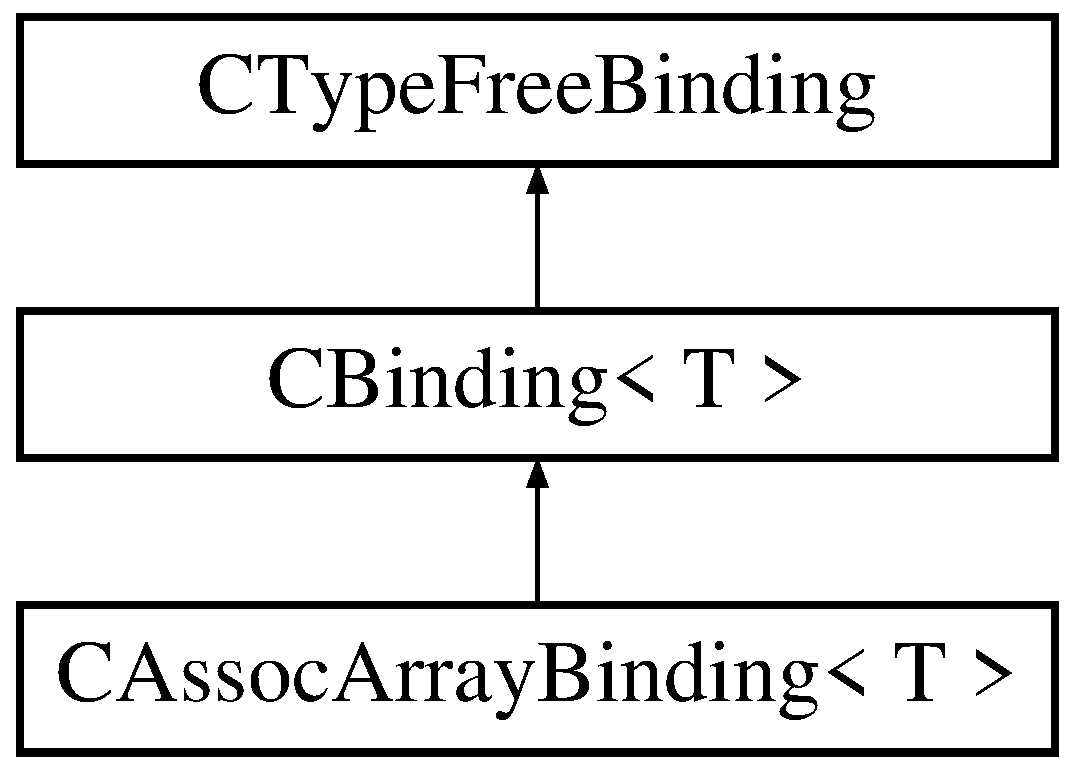
\includegraphics[height=3cm]{classCAssocArrayBinding}
\end{center}
\end{figure}
\subsection*{Public Methods}
\begin{CompactItemize}
\item 
{\bf CAssoc\-Array\-Binding} (const string \&r\-Name)
\item 
{\bf CAssoc\-Array\-Binding} (const char $\ast$p\-Name)
\item 
{\bf $\sim$CAssoc\-Array\-Binding} ()
\item 
map$<$ string, T $>$ {\bf get\-Array} () const
\begin{CompactList}\small\item\em $<$ Get entire map.\item\end{CompactList}\item 
map$<$ string, T $>$::iterator {\bf begin} ()
\item 
map$<$ string, T $>$::iterator {\bf end} ()
\item 
T \& {\bf operator[$\,$]} (const char $\ast$p\-Name)
\item 
T \& {\bf operator[$\,$]} (const string \&r\-Name)
\item 
map$<$ string, T $>$::iterator {\bf find} (const char $\ast$p\-Name)
\item 
map$<$ string, T $>$::iterator {\bf find} (const string \&r\-Name)
\item 
string {\bf get\-Name} () const
\item 
int {\bf get\-Type} () const
\item 
virtual void {\bf Init\-Bindings} ({\bf CTCLInterpreter} \&r\-Interp)
\item 
virtual void {\bf Commit} ({\bf CTCLInterpreter} \&r\-Interp)
\item 
virtual void {\bf Shutdown\-Bindings} ({\bf CTCLInterpreter} \&r\-Interp)
\item 
virtual void {\bf Dump} (int fd)
\end{CompactItemize}
\subsection*{Private Methods}
\begin{CompactItemize}
\item 
{\bf CAssoc\-Array\-Binding} (const CAssoc\-Array\-Binding \&rhs)
\item 
CAssoc\-Array\-Binding \& {\bf operator=} (const CAssoc\-Array\-Binding \&rhs)
\item 
int {\bf operator==} (const CAssoc\-Array\-Binding \&rhs)
\end{CompactItemize}
\subsection*{Private Attributes}
\begin{CompactItemize}
\item 
map$<$ string, T $>$ {\bf m\_\-Array}
\begin{CompactList}\small\item\em Data stored in this map.\item\end{CompactList}\item 
string {\bf m\_\-s\-Name}
\begin{CompactList}\small\item\em TCL Name of array.\item\end{CompactList}\item 
int {\bf m\_\-TCLVariable\-Type}
\begin{CompactList}\small\item\em Type of data in the array.\item\end{CompactList}\end{CompactItemize}


\subsection{Detailed Description}
\subsubsection*{template$<$class T$>$ class CAssoc\-Array\-Binding$<$ T $>$}

Encapsulates the configuration of an associative array. Associative arrays are arrays whose indices are strings rather than numbers. One use of associative arrays is to provide meaningful subscripts to configuration items. For example, suppose I want to store the thresholds for all of my 'detector' adc's. I might have an associative array named thresholds with subscripts which indicate detector segment and  subtype e.g. \char`\"{}seg1,de\char`\"{} could be an index. Some key properties of  associative arrays:\begin{CompactItemize}
\item 
One can iterate through the elements which have been given a value\item 
One can index by subscript, however if the element does not yet exist, it will be generated and the value will be that provided by the default constructor. Note that this is a null pointer for characters.\item 
There is no way to provide default values to elements in this clas. \end{CompactItemize}




Definition at line 326 of file CAssoc\-Array\-Binding.h.

\subsection{Constructor \& Destructor Documentation}
\index{CAssocArrayBinding@{CAssoc\-Array\-Binding}!CAssocArrayBinding@{CAssocArrayBinding}}
\index{CAssocArrayBinding@{CAssocArrayBinding}!CAssocArrayBinding@{CAssoc\-Array\-Binding}}
\subsubsection{\setlength{\rightskip}{0pt plus 5cm}template$<$class T$>$ CAssoc\-Array\-Binding$<$ T $>$::CAssoc\-Array\-Binding (const string \& {\em r\-Name})}\label{classCAssocArrayBinding_a0}


Constructs an associative array configured from a TCL array. The TCL array name is specified by a const string\& \begin{Desc}
\item[Parameters: ]\par
\begin{description}
\item[{\em 
r\-Name}]- Name of the configuration array. \end{description}
\end{Desc}


Definition at line 309 of file CAssoc\-Array\-Binding.cpp.

References CAssoc\-Array\-Binding$<$ T $>$::m\_\-TCLVariable\-Type, and CBinding$<$ T $>$::Variable\-Type().\index{CAssocArrayBinding@{CAssoc\-Array\-Binding}!CAssocArrayBinding@{CAssocArrayBinding}}
\index{CAssocArrayBinding@{CAssocArrayBinding}!CAssocArrayBinding@{CAssoc\-Array\-Binding}}
\subsubsection{\setlength{\rightskip}{0pt plus 5cm}template$<$class T$>$ CAssoc\-Array\-Binding$<$ T $>$::CAssoc\-Array\-Binding (const char $\ast$ {\em p\-Name})}\label{classCAssocArrayBinding_a1}


Constructs an associative array configured from a TCL array. The TCL array name is speicified by a const char$\ast$ \begin{Desc}
\item[Parameters: ]\par
\begin{description}
\item[{\em 
p\-Name}]- Name of the configuration array. \end{description}
\end{Desc}


Definition at line 322 of file CAssoc\-Array\-Binding.cpp.

References CAssoc\-Array\-Binding$<$ T $>$::m\_\-TCLVariable\-Type, and CBinding$<$ T $>$::Variable\-Type().\index{CAssocArrayBinding@{CAssoc\-Array\-Binding}!~CAssocArrayBinding@{$\sim$CAssocArrayBinding}}
\index{~CAssocArrayBinding@{$\sim$CAssocArrayBinding}!CAssocArrayBinding@{CAssoc\-Array\-Binding}}
\subsubsection{\setlength{\rightskip}{0pt plus 5cm}template$<$class T$>$ CAssoc\-Array\-Binding$<$ T $>$::$\sim$CAssoc\-Array\-Binding ()}\label{classCAssocArrayBinding_a2}


The destructor will need to delete storage associated with character entries in the map. 

Definition at line 334 of file CAssoc\-Array\-Binding.cpp.

References CAssoc\-Array\-Binding$<$ T $>$::m\_\-Array, and CAssoc\-Array\-Binding$<$ T $>$::m\_\-TCLVariable\-Type.\index{CAssocArrayBinding@{CAssoc\-Array\-Binding}!CAssocArrayBinding@{CAssocArrayBinding}}
\index{CAssocArrayBinding@{CAssocArrayBinding}!CAssocArrayBinding@{CAssoc\-Array\-Binding}}
\subsubsection{\setlength{\rightskip}{0pt plus 5cm}template$<$class T$>$ CAssoc\-Array\-Binding$<$ T $>$::CAssoc\-Array\-Binding (const CAssoc\-Array\-Binding$<$ T $>$ \& {\em rhs})\hspace{0.3cm}{\tt  [private]}}\label{classCAssocArrayBinding_c0}




\subsection{Member Function Documentation}
\index{CAssocArrayBinding@{CAssoc\-Array\-Binding}!begin@{begin}}
\index{begin@{begin}!CAssocArrayBinding@{CAssoc\-Array\-Binding}}
\subsubsection{\setlength{\rightskip}{0pt plus 5cm}template$<$class T$>$ map$<$string,T$>$::iterator CAssoc\-Array\-Binding$<$ T $>$::begin ()\hspace{0.3cm}{\tt  [inline]}}\label{classCAssocArrayBinding_a4}




Definition at line 350 of file CAssoc\-Array\-Binding.h.

References CAssoc\-Array\-Binding$<$ T $>$::m\_\-Array.\index{CAssocArrayBinding@{CAssoc\-Array\-Binding}!Commit@{Commit}}
\index{Commit@{Commit}!CAssocArrayBinding@{CAssoc\-Array\-Binding}}
\subsubsection{\setlength{\rightskip}{0pt plus 5cm}template$<$class T$>$ void CAssoc\-Array\-Binding$<$ T $>$::Commit ({\bf CTCLInterpreter} \& {\em r\-Interp})\hspace{0.3cm}{\tt  [virtual]}}\label{classCAssocArrayBinding_a13}


Commits the bindings to the array. In this case we will determine the set of indices the variable has (by running a string script of the form \char`\"{}array names m\_\-s\-Name\char`\"{}, and fetching the results from the result string. For each item in the TCL array an item is created in the  m\_\-Array. Note that if the type is TCL\_\-BIND\_\-STRING, dynamic memory is allocated to hold the result string. \begin{Desc}
\item[Parameters: ]\par
\begin{description}
\item[{\em 
r\-Interp}]- the interpreter which read in the config file. Used to fetch variable strings etc. \end{description}
\end{Desc}


Implements {\bf CBinding$<$ T $>$} {\rm (p.\,\pageref{classCBinding_a1})}.

Definition at line 371 of file CAssoc\-Array\-Binding.cpp.

References CTCLInterpreter::Expr\-Boolean(), CTCLInterpreter::Expr\-Double(), CTCLInterpreter::Expr\-Long(), CTCLInterpreter::get\-Interpreter(), CTCLInterpreter::Global\-Eval(), CAssoc\-Array\-Binding$<$ T $>$::m\_\-Array, CAssoc\-Array\-Binding$<$ T $>$::m\_\-s\-Name, CTCLList::Split(), and String\-Array.\index{CAssocArrayBinding@{CAssoc\-Array\-Binding}!Dump@{Dump}}
\index{Dump@{Dump}!CAssocArrayBinding@{CAssoc\-Array\-Binding}}
\subsubsection{\setlength{\rightskip}{0pt plus 5cm}template$<$class T$>$ void CAssoc\-Array\-Binding$<$ T $>$::Dump (int {\em fd})\hspace{0.3cm}{\tt  [virtual]}}\label{classCAssocArrayBinding_a15}


Dumps the contents of the array out in a form which allows the array to be recovered by reading the file. \begin{Desc}
\item[Parameters: ]\par
\begin{description}
\item[{\em 
fd}]- A file descriptor on which to write this data. \end{description}
\end{Desc}


Implements {\bf CBinding$<$ T $>$} {\rm (p.\,\pageref{classCBinding_a2})}.

Definition at line 469 of file CAssoc\-Array\-Binding.cpp.

References CBinding$<$ T $>$::Item\-To\-String(), CAssoc\-Array\-Binding$<$ T $>$::m\_\-Array, and CAssoc\-Array\-Binding$<$ T $>$::m\_\-s\-Name.\index{CAssocArrayBinding@{CAssoc\-Array\-Binding}!end@{end}}
\index{end@{end}!CAssocArrayBinding@{CAssoc\-Array\-Binding}}
\subsubsection{\setlength{\rightskip}{0pt plus 5cm}template$<$class T$>$ map$<$string,T$>$::iterator CAssoc\-Array\-Binding$<$ T $>$::end ()\hspace{0.3cm}{\tt  [inline]}}\label{classCAssocArrayBinding_a5}




Definition at line 353 of file CAssoc\-Array\-Binding.h.

References CAssoc\-Array\-Binding$<$ T $>$::m\_\-Array.\index{CAssocArrayBinding@{CAssoc\-Array\-Binding}!find@{find}}
\index{find@{find}!CAssocArrayBinding@{CAssoc\-Array\-Binding}}
\subsubsection{\setlength{\rightskip}{0pt plus 5cm}template$<$class T$>$ map$<$string,T$>$::iterator CAssoc\-Array\-Binding$<$ T $>$::find (const string \& {\em r\-Name})\hspace{0.3cm}{\tt  [inline]}}\label{classCAssocArrayBinding_a9}




Definition at line 366 of file CAssoc\-Array\-Binding.h.

References CAssoc\-Array\-Binding$<$ T $>$::m\_\-Array.\index{CAssocArrayBinding@{CAssoc\-Array\-Binding}!find@{find}}
\index{find@{find}!CAssocArrayBinding@{CAssoc\-Array\-Binding}}
\subsubsection{\setlength{\rightskip}{0pt plus 5cm}template$<$class T$>$ map$<$string,T$>$::iterator CAssoc\-Array\-Binding$<$ T $>$::find (const char $\ast$ {\em p\-Name})\hspace{0.3cm}{\tt  [inline]}}\label{classCAssocArrayBinding_a8}




Definition at line 363 of file CAssoc\-Array\-Binding.h.

References CAssoc\-Array\-Binding$<$ T $>$::m\_\-Array.\index{CAssocArrayBinding@{CAssoc\-Array\-Binding}!getArray@{getArray}}
\index{getArray@{getArray}!CAssocArrayBinding@{CAssoc\-Array\-Binding}}
\subsubsection{\setlength{\rightskip}{0pt plus 5cm}template$<$class T$>$ map$<$string,T$>$ CAssoc\-Array\-Binding$<$ T $>$::get\-Array () const\hspace{0.3cm}{\tt  [inline]}}\label{classCAssocArrayBinding_a3}


$<$ Get entire map.



Definition at line 346 of file CAssoc\-Array\-Binding.h.

References CAssoc\-Array\-Binding$<$ T $>$::m\_\-Array.\index{CAssocArrayBinding@{CAssoc\-Array\-Binding}!getName@{getName}}
\index{getName@{getName}!CAssocArrayBinding@{CAssoc\-Array\-Binding}}
\subsubsection{\setlength{\rightskip}{0pt plus 5cm}template$<$class T$>$ string CAssoc\-Array\-Binding$<$ T $>$::get\-Name () const\hspace{0.3cm}{\tt  [inline]}}\label{classCAssocArrayBinding_a10}




Definition at line 370 of file CAssoc\-Array\-Binding.h.

References CAssoc\-Array\-Binding$<$ T $>$::m\_\-s\-Name.\index{CAssocArrayBinding@{CAssoc\-Array\-Binding}!getType@{getType}}
\index{getType@{getType}!CAssocArrayBinding@{CAssoc\-Array\-Binding}}
\subsubsection{\setlength{\rightskip}{0pt plus 5cm}template$<$class T$>$ int CAssoc\-Array\-Binding$<$ T $>$::get\-Type () const\hspace{0.3cm}{\tt  [inline]}}\label{classCAssocArrayBinding_a11}




Definition at line 374 of file CAssoc\-Array\-Binding.h.

References CAssoc\-Array\-Binding$<$ T $>$::m\_\-TCLVariable\-Type.\index{CAssocArrayBinding@{CAssoc\-Array\-Binding}!InitBindings@{InitBindings}}
\index{InitBindings@{InitBindings}!CAssocArrayBinding@{CAssoc\-Array\-Binding}}
\subsubsection{\setlength{\rightskip}{0pt plus 5cm}template$<$class T$>$ void CAssoc\-Array\-Binding$<$ T $>$::Init\-Bindings ({\bf CTCLInterpreter} \& {\em r\-Interp})\hspace{0.3cm}{\tt  [virtual]}}\label{classCAssocArrayBinding_a12}


Initialize the bindings prior to reading in the configuration file. for this class the actual binding operation is done in the commit phase so this is a no-op. \begin{Desc}
\item[Parameters: ]\par
\begin{description}
\item[{\em 
r\-Interp}]- Referencers the TCL interpreter which will be used to read in the configuration file. \end{description}
\end{Desc}


Implements {\bf CBinding$<$ T $>$} {\rm (p.\,\pageref{classCBinding_a0})}.

Definition at line 354 of file CAssoc\-Array\-Binding.cpp.\index{CAssocArrayBinding@{CAssoc\-Array\-Binding}!operator=@{operator=}}
\index{operator=@{operator=}!CAssocArrayBinding@{CAssoc\-Array\-Binding}}
\subsubsection{\setlength{\rightskip}{0pt plus 5cm}template$<$class T$>$ CAssoc\-Array\-Binding\& CAssoc\-Array\-Binding$<$ T $>$::operator= (const CAssoc\-Array\-Binding$<$ T $>$ \& {\em rhs})\hspace{0.3cm}{\tt  [private]}}\label{classCAssocArrayBinding_c1}


\index{CAssocArrayBinding@{CAssoc\-Array\-Binding}!operator==@{operator==}}
\index{operator==@{operator==}!CAssocArrayBinding@{CAssoc\-Array\-Binding}}
\subsubsection{\setlength{\rightskip}{0pt plus 5cm}template$<$class T$>$ int CAssoc\-Array\-Binding$<$ T $>$::operator== (const CAssoc\-Array\-Binding$<$ T $>$ \& {\em rhs})\hspace{0.3cm}{\tt  [private]}}\label{classCAssocArrayBinding_c2}


\index{CAssocArrayBinding@{CAssoc\-Array\-Binding}!operator[]@{operator[]}}
\index{operator[]@{operator[]}!CAssocArrayBinding@{CAssoc\-Array\-Binding}}
\subsubsection{\setlength{\rightskip}{0pt plus 5cm}template$<$class T$>$ T\& CAssoc\-Array\-Binding$<$ T $>$::operator[$\,$] (const string \& {\em r\-Name})\hspace{0.3cm}{\tt  [inline]}}\label{classCAssocArrayBinding_a7}




Definition at line 360 of file CAssoc\-Array\-Binding.h.

References CAssoc\-Array\-Binding$<$ T $>$::m\_\-Array.\index{CAssocArrayBinding@{CAssoc\-Array\-Binding}!operator[]@{operator[]}}
\index{operator[]@{operator[]}!CAssocArrayBinding@{CAssoc\-Array\-Binding}}
\subsubsection{\setlength{\rightskip}{0pt plus 5cm}template$<$class T$>$ T\& CAssoc\-Array\-Binding$<$ T $>$::operator[$\,$] (const char $\ast$ {\em p\-Name})\hspace{0.3cm}{\tt  [inline]}}\label{classCAssocArrayBinding_a6}




Definition at line 356 of file CAssoc\-Array\-Binding.h.

References CAssoc\-Array\-Binding$<$ T $>$::m\_\-Array.\index{CAssocArrayBinding@{CAssoc\-Array\-Binding}!ShutdownBindings@{ShutdownBindings}}
\index{ShutdownBindings@{ShutdownBindings}!CAssocArrayBinding@{CAssoc\-Array\-Binding}}
\subsubsection{\setlength{\rightskip}{0pt plus 5cm}template$<$class T$>$ void CAssoc\-Array\-Binding$<$ T $>$::Shutdown\-Bindings ({\bf CTCLInterpreter} \& {\em r\-Interp})\hspace{0.3cm}{\tt  [virtual]}}\label{classCAssocArrayBinding_a14}


Closes out whatever needs closing prior to deleting the interpreter which was used to read the configuration file. In this case, no action is taken as the 'binding' is done at commit time and no real connection is made between the interpreter and the array. \begin{Desc}
\item[Parameters: ]\par
\begin{description}
\item[{\em 
r\-Interp}]- Interpreter which read the config file. \end{description}
\end{Desc}


Implements {\bf CType\-Free\-Binding} {\rm (p.\,\pageref{classCTypeFreeBinding_a2})}.

Definition at line 459 of file CAssoc\-Array\-Binding.cpp.

\subsection{Member Data Documentation}
\index{CAssocArrayBinding@{CAssoc\-Array\-Binding}!m_Array@{m\_\-Array}}
\index{m_Array@{m\_\-Array}!CAssocArrayBinding@{CAssoc\-Array\-Binding}}
\subsubsection{\setlength{\rightskip}{0pt plus 5cm}template$<$class T$>$ map$<$string,T$>$ CAssoc\-Array\-Binding$<$ T $>$::m\_\-Array\hspace{0.3cm}{\tt  [private]}}\label{classCAssocArrayBinding_o0}


Data stored in this map.



Definition at line 330 of file CAssoc\-Array\-Binding.h.

Referenced by CAssoc\-Array\-Binding$<$ T $>$::begin(), CAssoc\-Array\-Binding$<$ T $>$::Commit(), CAssoc\-Array\-Binding$<$ T $>$::Dump(), CAssoc\-Array\-Binding$<$ T $>$::end(), CAssoc\-Array\-Binding$<$ T $>$::find(), CAssoc\-Array\-Binding$<$ T $>$::get\-Array(), CAssoc\-Array\-Binding$<$ T $>$::operator[$\,$](), and CAssoc\-Array\-Binding$<$ T $>$::$\sim$CAssoc\-Array\-Binding().\index{CAssocArrayBinding@{CAssoc\-Array\-Binding}!m_sName@{m\_\-sName}}
\index{m_sName@{m\_\-sName}!CAssocArrayBinding@{CAssoc\-Array\-Binding}}
\subsubsection{\setlength{\rightskip}{0pt plus 5cm}template$<$class T$>$ string CAssoc\-Array\-Binding$<$ T $>$::m\_\-s\-Name\hspace{0.3cm}{\tt  [private]}}\label{classCAssocArrayBinding_o1}


TCL Name of array.



Definition at line 331 of file CAssoc\-Array\-Binding.h.

Referenced by CAssoc\-Array\-Binding$<$ T $>$::Commit(), CAssoc\-Array\-Binding$<$ T $>$::Dump(), and CAssoc\-Array\-Binding$<$ T $>$::get\-Name().\index{CAssocArrayBinding@{CAssoc\-Array\-Binding}!m_TCLVariableType@{m\_\-TCLVariableType}}
\index{m_TCLVariableType@{m\_\-TCLVariableType}!CAssocArrayBinding@{CAssoc\-Array\-Binding}}
\subsubsection{\setlength{\rightskip}{0pt plus 5cm}template$<$class T$>$ int CAssoc\-Array\-Binding$<$ T $>$::m\_\-TCLVariable\-Type\hspace{0.3cm}{\tt  [private]}}\label{classCAssocArrayBinding_o2}


Type of data in the array.



Definition at line 332 of file CAssoc\-Array\-Binding.h.

Referenced by CAssoc\-Array\-Binding$<$ T $>$::CAssoc\-Array\-Binding(), CAssoc\-Array\-Binding$<$ T $>$::get\-Type(), and CAssoc\-Array\-Binding$<$ T $>$::$\sim$CAssoc\-Array\-Binding().

The documentation for this class was generated from the following files:\begin{CompactItemize}
\item 
{\bf CAssoc\-Array\-Binding.h}\item 
{\bf CAssoc\-Array\-Binding.cpp}\end{CompactItemize}

\section{CBinding$<$ T $>$  Class Template Reference}
\label{classCBinding}\index{CBinding@{CBinding}}
{\tt \#include $<$CBinding.h$>$}

Inheritance diagram for CBinding$<$ T $>$::\begin{figure}[H]
\begin{center}
\leavevmode
\includegraphics[height=3cm]{classCBinding}
\end{center}
\end{figure}
\subsection*{Public Methods}
\begin{CompactItemize}
\item 
virtual void {\bf Init\-Bindings} ({\bf CTCLInterpreter} \&r\-Interp)=0
\item 
virtual void {\bf Commit} ({\bf CTCLInterpreter} \&r\-Interp)=0
\item 
virtual void {\bf Dump} (int fd)=0
\item 
int {\bf Variable\-Type} (T item)
\item 
string {\bf Item\-To\-String} (T Item)
\end{CompactItemize}


\subsection{Detailed Description}
\subsubsection*{template$<$class T$>$ class CBinding$<$ T $>$}

This is an abstract base class for the Tcl configuration manager's bindings subsystem. interfaces for the functions required of all bindings objects are defined as pure virtual member functions. 



Definition at line 322 of file CBinding.h.

\subsection{Member Function Documentation}
\index{CBinding@{CBinding}!Commit@{Commit}}
\index{Commit@{Commit}!CBinding@{CBinding}}
\subsubsection{\setlength{\rightskip}{0pt plus 5cm}template$<$class T$>$ virtual void CBinding$<$ T $>$::Commit ({\bf CTCLInterpreter} \& {\em r\-Interp})\hspace{0.3cm}{\tt  [pure virtual]}}\label{classCBinding_a1}


This function is called just after a configuration script or set of  configuration scripts have been read to perform any actions required to commit the read in Tcl values to the variables. For example, an associative array bindings might need to fetch the individual values from Tcl array elements. \begin{Desc}
\item[Parameters: ]\par
\begin{description}
\item[{\em 
r\-Interp}]- The interpreter in which the config script was read. \end{description}
\end{Desc}


Implements {\bf CType\-Free\-Binding} {\rm (p.\,\pageref{classCTypeFreeBinding_a1})}.

Implemented in {\bf CArray\-Binding$<$ T $>$} {\rm (p.\,\pageref{classCArrayBinding_a11})}, {\bf CAssoc\-Array\-Binding$<$ T $>$} {\rm (p.\,\pageref{classCAssocArrayBinding_a13})}, and {\bf CVariable\-Binding$<$ T $>$} {\rm (p.\,\pageref{classCVariableBinding_a14})}.\index{CBinding@{CBinding}!Dump@{Dump}}
\index{Dump@{Dump}!CBinding@{CBinding}}
\subsubsection{\setlength{\rightskip}{0pt plus 5cm}template$<$class T$>$ virtual void CBinding$<$ T $>$::Dump (int {\em fd})\hspace{0.3cm}{\tt  [pure virtual]}}\label{classCBinding_a2}


This function is called just prior to deleting the interpreter. Any cleanup actions required by the binding should be done at this point. For example, if Init mapped a C variable to a TCL variable, that mapping should be broken. \begin{Desc}
\item[Parameters: ]\par
\begin{description}
\item[{\em 
r\-Interp}]- The interpreter about to be deleted. virtual void {\bf Shutdown\-Bindings}(CTCLInterpreter\& r\-Interp) {\rm (p.\,\pageref{classCTypeFreeBinding_a2})}= 0; /$\ast$! This function is called to write the set of Tcl commands required to duplicate the current state. Note that this may not be identical to the set of commands which produced the configuration. \end{description}
\end{Desc}


Implements {\bf CType\-Free\-Binding} {\rm (p.\,\pageref{classCTypeFreeBinding_a3})}.

Implemented in {\bf CArray\-Binding$<$ T $>$} {\rm (p.\,\pageref{classCArrayBinding_a13})}, {\bf CAssoc\-Array\-Binding$<$ T $>$} {\rm (p.\,\pageref{classCAssocArrayBinding_a15})}, and {\bf CVariable\-Binding$<$ T $>$} {\rm (p.\,\pageref{classCVariableBinding_a16})}.\index{CBinding@{CBinding}!InitBindings@{InitBindings}}
\index{InitBindings@{InitBindings}!CBinding@{CBinding}}
\subsubsection{\setlength{\rightskip}{0pt plus 5cm}template$<$class T$>$ virtual void CBinding$<$ T $>$::Init\-Bindings ({\bf CTCLInterpreter} \& {\em r\-Interp})\hspace{0.3cm}{\tt  [pure virtual]}}\label{classCBinding_a0}


This function will be called just prior to reading in a configuration file. The Tcl Interpreter has been set up and initialized. The Init function can do any preparation required by the binding prior to readin (e.g. a simple binding $>$might$<$ bind the contained variable to a Tcl variable \begin{Desc}
\item[Parameters: ]\par
\begin{description}
\item[{\em 
r\-Interp}]- The interpreter on which the config script will be read. \end{description}
\end{Desc}


Implements {\bf CType\-Free\-Binding} {\rm (p.\,\pageref{classCTypeFreeBinding_a0})}.

Implemented in {\bf CArray\-Binding$<$ T $>$} {\rm (p.\,\pageref{classCArrayBinding_a10})}, {\bf CAssoc\-Array\-Binding$<$ T $>$} {\rm (p.\,\pageref{classCAssocArrayBinding_a12})}, and {\bf CVariable\-Binding$<$ T $>$} {\rm (p.\,\pageref{classCVariableBinding_a13})}.\index{CBinding@{CBinding}!ItemToString@{ItemToString}}
\index{ItemToString@{ItemToString}!CBinding@{CBinding}}
\subsubsection{\setlength{\rightskip}{0pt plus 5cm}template$<$class T$>$ string CBinding$<$ T $>$::Item\-To\-String (T {\em Item})\hspace{0.3cm}{\tt  [inline]}}\label{classCBinding_a4}


Item to string conversion: Converts an item of type T to  its string representation.  \begin{Desc}
\item[Parameters: ]\par
\begin{description}
\item[{\em 
item}]- item to convert. \end{description}
\end{Desc}
\begin{Desc}
\item[Exceptions: ]\par
\begin{description}
\item[{\em 
{\bf CRange\-Error} {\rm (p.\,\pageref{classCRangeError})}}] - no type match \end{description}
\end{Desc}
\begin{Desc}
\item[{\bf Bug: }]\par
 Should invent a bad type exception and throw it. \end{Desc}
 

Definition at line 390 of file CBinding.h.

Referenced by CVariable\-Binding$<$ T $>$::Dump(), CAssoc\-Array\-Binding$<$ T $>$::Dump(), and CArray\-Binding$<$ T $>$::Dump().\index{CBinding@{CBinding}!VariableType@{VariableType}}
\index{VariableType@{VariableType}!CBinding@{CBinding}}
\subsubsection{\setlength{\rightskip}{0pt plus 5cm}template$<$class T$>$ int CBinding$<$ T $>$::Variable\-Type (T {\em item})\hspace{0.3cm}{\tt  [inline]}}\label{classCBinding_a3}


Returns the TCL code for the type of variable being bound to: This can be one of:\begin{CompactItemize}
\item 
TCL\_\-LINK\_\-INT - Variable is an integer.\item 
TCL\_\-LINK\_\-DOUBLE - Variable is a double precision.\item 
TCL\_\-LINK\_\-BOOLEAN - Variable is a boolean.\item 
TCL\_\-LINK\_\-STRING - Variable is a char$\ast$.\end{CompactItemize}
\begin{Desc}
\item[Parameters: ]\par
\begin{description}
\item[{\em 
item}]- A variable of type T.\end{description}
\end{Desc}
\begin{Desc}
\item[Exceptions: ]\par
\begin{description}
\item[{\em 
{\bf CRange\-Error} {\rm (p.\,\pageref{classCRangeError})}}] - no neat match.\end{description}
\end{Desc}


\begin{Desc}
\item[{\bf Bug: }]\par
Really should invent a bad type exception and throw it instead\end{Desc}
 

Definition at line 372 of file CBinding.h.

Referenced by CAssoc\-Array\-Binding$<$ T $>$::CAssoc\-Array\-Binding().

The documentation for this class was generated from the following file:\begin{CompactItemize}
\item 
{\bf CBinding.h}\end{CompactItemize}

\section{CBuffer\-Event$<$ T $>$  Class Template Reference}
\label{classCBufferEvent}\index{CBufferEvent@{CBuffer\-Event}}
$\backslash$class: CBuffer\-Event $\backslash$file: {\bf CBuffer\-Event.h}. 


{\tt \#include $<$CBuffer\-Event.h$>$}

Inheritance diagram for CBuffer\-Event$<$ T $>$::\begin{figure}[H]
\begin{center}
\leavevmode
\includegraphics[height=4cm]{classCBufferEvent}
\end{center}
\end{figure}
\subsection*{Public Methods}
\begin{CompactItemize}
\item 
{\bf CBuffer\-Event} ()
\begin{CompactList}\small\item\em Anonymous buffer event.\item\end{CompactList}\item 
{\bf CBuffer\-Event} (const char $\ast$p\-Name)
\begin{CompactList}\small\item\em Named event with char$\ast$ name.\item\end{CompactList}\item 
{\bf CBuffer\-Event} (const string \&r\-Name)
\begin{CompactList}\small\item\em Named event with string name.\item\end{CompactList}\item 
{\bf $\sim$CBuffer\-Event} ()
\begin{CompactList}\small\item\em Destroy the event.\item\end{CompactList}\item 
list$<$ {\bf Add\-Link\-Request} $>$ {\bf get\-Pending\-Add\-Queue} () const
\item 
list$<$ {\bf Add\-Link\-Request} $>$ {\bf get\-Pending\-Delete\-Queue} () const
\item 
{\bf CBuffer\-Monitor}$<$ T $>$ \& {\bf get\-Monitor} ()
\begin{CompactList}\small\item\em Allow manipulation of the event monitor:.\item\end{CompactList}\item 
{\bf CBuffer\-Reactor}$<$ T $>$ \& {\bf get\-Reactor} ()
\begin{CompactList}\small\item\em Allow manipulation of the event reactor:.\item\end{CompactList}\item 
void {\bf Add\-Link} (const string \&url, unsigned int tag, unsigned int mask=ALLBITS\_\-MASK, int reliability=COS\_\-RELIABLE)
\item 
void {\bf Delete\-Link} (const string \&url, unsigned int tag, unsigned int mask=ALLBITS\_\-MASK, int reliability=COS\_\-RELIABLE)
\item 
virtual void {\bf On\-Buffer} (Pointer$<$ DAQBuffer$<$ T $>$, T $>$ \&p\-Buffer)
\item 
virtual void {\bf On\-Timeout} ()
\item 
virtual void {\bf set\-Buffer\-Tag} (int tag)
\item 
virtual void {\bf set\-Buffer\-Mask} (int mask)
\item 
virtual string {\bf Describe\-Self} ()
\end{CompactItemize}
\subsection*{Protected Methods}
\begin{CompactItemize}
\item 
virtual void {\bf Process\-Queues} ()
\item 
void {\bf Process\-Add\-Queue} ()
\item 
void {\bf Process\-Del\-Queue} ()
\item 
string {\bf Queue\-Entry\-To\-String} ({\bf Add\-Link\-Request} \&r\-Entry)
\end{CompactItemize}
\subsection*{Private Methods}
\begin{CompactItemize}
\item 
{\bf CBuffer\-Event} (const CBuffer\-Event \&rhs)
\item 
CBuffer\-Event \& {\bf operator=} (const CBuffer\-Event \&rhs)
\item 
int {\bf operator==} (const CBuffer\-Event \&rhs)
\end{CompactItemize}
\subsection*{Private Attributes}
\begin{CompactItemize}
\item 
list$<$ {\bf Add\-Link\-Request} $>$ {\bf m\_\-Add\-Queue}
\begin{CompactList}\small\item\em Requests to add links go here.\item\end{CompactList}\item 
list$<$ {\bf Add\-Link\-Request} $>$ {\bf m\_\-Del\-Queue}
\begin{CompactList}\small\item\em Requests to delete links go here.\item\end{CompactList}\item 
{\bf CBuffer\-Monitor}$<$ T $>$ \& {\bf m\_\-r\-Monitor}
\begin{CompactList}\small\item\em Monitors the input links.\item\end{CompactList}\item 
{\bf CGeneric\-Buffer\-Reactor}$<$ T $>$ \& {\bf m\_\-r\-Reactor}
\begin{CompactList}\small\item\em Reacts to the input links.\item\end{CompactList}\end{CompactItemize}


\subsection{Detailed Description}
\subsubsection*{template$<$class T$>$ class CBuffer\-Event$<$ T $>$}

$\backslash$class: CBuffer\-Event $\backslash$file: {\bf CBuffer\-Event.h}.

Provides an ABC for building application level objects to react to Spectro\-Daq Buffers. This is an abstract, templated class which is templated by the type of buffer whch can be received. Note that depending on how this is constructed,, The object can handle alarm events instead of data buffers. 



Definition at line 342 of file CBuffer\-Event.h.

\subsection{Constructor \& Destructor Documentation}
\index{CBufferEvent@{CBuffer\-Event}!CBufferEvent@{CBufferEvent}}
\index{CBufferEvent@{CBufferEvent}!CBufferEvent@{CBuffer\-Event}}
\subsubsection{\setlength{\rightskip}{0pt plus 5cm}template$<$class T$>$ CBuffer\-Event$<$ T $>$::CBuffer\-Event ()}\label{classCBufferEvent_a0}


Anonymous buffer event.

Construct an anonymous event. The monitor is a standard buffer monitor, the event readctor is a {\bf CGeneric\-Buffer\-Reactor} {\rm (p.\,\pageref{classCBufferEvent_1_1CGenericBufferReactor})}. 

Definition at line 359 of file CBuffer\-Event.cpp.

References CBuffer\-Event$<$ T $>$::get\-Monitor(), CBuffer\-Event$<$ T $>$::get\-Reactor(), CBuffer\-Event$<$ T $>$::m\_\-r\-Monitor, and CBuffer\-Event$<$ T $>$::m\_\-r\-Reactor.\index{CBufferEvent@{CBuffer\-Event}!CBufferEvent@{CBufferEvent}}
\index{CBufferEvent@{CBufferEvent}!CBufferEvent@{CBuffer\-Event}}
\subsubsection{\setlength{\rightskip}{0pt plus 5cm}template$<$class T$>$ CBuffer\-Event$<$ T $>$::CBuffer\-Event (const char $\ast$ {\em p\-Name})}\label{classCBufferEvent_a1}


Named event with char$\ast$ name.

Called to create a named buffer event when the name is a char$\ast$ string: 

Definition at line 371 of file CBuffer\-Event.cpp.\index{CBufferEvent@{CBuffer\-Event}!CBufferEvent@{CBufferEvent}}
\index{CBufferEvent@{CBufferEvent}!CBufferEvent@{CBuffer\-Event}}
\subsubsection{\setlength{\rightskip}{0pt plus 5cm}template$<$class T$>$ CBuffer\-Event$<$ T $>$::CBuffer\-Event (const string \& {\em r\-Name})}\label{classCBufferEvent_a2}


Named event with string name.

Called to create a named buffer event when the name is an stl string. 

Definition at line 383 of file CBuffer\-Event.cpp.\index{CBufferEvent@{CBuffer\-Event}!~CBufferEvent@{$\sim$CBufferEvent}}
\index{~CBufferEvent@{$\sim$CBufferEvent}!CBufferEvent@{CBuffer\-Event}}
\subsubsection{\setlength{\rightskip}{0pt plus 5cm}template$<$class T$>$ CBuffer\-Event$<$ T $>$::$\sim$CBuffer\-Event ()}\label{classCBufferEvent_a3}


Destroy the event.

Destroy the buffer event: 

Definition at line 395 of file CBuffer\-Event.cpp.

References CBuffer\-Event$<$ T $>$::m\_\-r\-Monitor, and CBuffer\-Event$<$ T $>$::m\_\-r\-Reactor.\index{CBufferEvent@{CBuffer\-Event}!CBufferEvent@{CBufferEvent}}
\index{CBufferEvent@{CBufferEvent}!CBufferEvent@{CBuffer\-Event}}
\subsubsection{\setlength{\rightskip}{0pt plus 5cm}template$<$class T$>$ CBuffer\-Event$<$ T $>$::CBuffer\-Event (const CBuffer\-Event$<$ T $>$ \& {\em rhs})\hspace{0.3cm}{\tt  [private]}}\label{classCBufferEvent_c0}




\subsection{Member Function Documentation}
\index{CBufferEvent@{CBuffer\-Event}!AddLink@{AddLink}}
\index{AddLink@{AddLink}!CBufferEvent@{CBuffer\-Event}}
\subsubsection{\setlength{\rightskip}{0pt plus 5cm}template$<$class T$>$ void CBuffer\-Event$<$ T $>$::Add\-Link (const string \& {\em url}, unsigned int {\em tag}, unsigned int {\em mask} = ALLBITS\_\-MASK, int {\em reliability} = COS\_\-RELIABLE)}\label{classCBufferEvent_a8}


Called to add a link. The link must be added in the context of the event's thread or else buffers will not be received. The link addition requests, are therefore queued to the list of pending link add requests m\_\-Add\-Queue. This must be done in a globally synchronized way. \begin{Desc}
\item[Parameters: ]\par
\begin{description}
\item[{\em 
url}]- The url of the host to link data from. \item[{\em 
tag}]- The match tag (after mask has been applied). \item[{\em 
mask}]- Receive mask to be anded with the buffer type. \item[{\em 
reliability}]- Can be:\begin{CompactItemize}
\item 
COS\_\-RELIABLE - Indicates the link should recieve all buffers.\item 
COS\_\-UNRELIABLE - Indicates the link need not receive all buffers. \end{CompactItemize}
\end{description}
\end{Desc}


Definition at line 415 of file CBuffer\-Event.cpp.

References CApplication\-Serializer::get\-Instance(), CThread\-Recursive\-Mutex::Lock(), CBuffer\-Event$<$ T $>$::m\_\-Add\-Queue, and CThread\-Recursive\-Mutex::Un\-Lock().\index{CBufferEvent@{CBuffer\-Event}!DeleteLink@{DeleteLink}}
\index{DeleteLink@{DeleteLink}!CBufferEvent@{CBuffer\-Event}}
\subsubsection{\setlength{\rightskip}{0pt plus 5cm}template$<$class T$>$ void CBuffer\-Event$<$ T $>$::Delete\-Link (const string \& {\em url}, unsigned int {\em tag}, unsigned int {\em mask} = ALLBITS\_\-MASK, int {\em reliability} = COS\_\-RELIABLE)}\label{classCBufferEvent_a9}


Queues a link deletion. Links are deleted by matching URL, mask and  reliabilities. The deletion must be done in the context of the thread receiving buffers. Therefore, this member just synchronizes with the application global mutex, and adds the link description to the pending deletion queue. Next time the buffer receiving thread executes (either because a buffer arrives or because the wait times out), new links will be made and old links deleted.\begin{Desc}
\item[Parameters: ]\par
\begin{description}
\item[{\em 
url}]- The URL describing the server which we will be getting buffers from. \item[{\em 
tag}]- The buffer tag. \item[{\em 
mask}]- Mask to be applied to the inbound buffer. \item[{\em 
reliability}]- Can be any of:\begin{CompactItemize}
\item 
COS\_\-RELIABLE - All matching buffers are delivered.\item 
COS\_\-UNRELIABLE - Matching buffers are only deliverd if receive has no 'active' buffers. \end{CompactItemize}
\end{description}
\end{Desc}


Definition at line 451 of file CBuffer\-Event.cpp.

References CApplication\-Serializer::get\-Instance(), CThread\-Recursive\-Mutex::Lock(), CBuffer\-Event$<$ T $>$::m\_\-Del\-Queue, CBuffer\-Event$<$ T $>$::Add\-Link\-Request::s\_\-mask, CBuffer\-Event$<$ T $>$::Add\-Link\-Request::s\_\-tag, CBuffer\-Event$<$ T $>$::Add\-Link\-Request::s\_\-url, and CThread\-Recursive\-Mutex::Un\-Lock().\index{CBufferEvent@{CBuffer\-Event}!DescribeSelf@{DescribeSelf}}
\index{DescribeSelf@{DescribeSelf}!CBufferEvent@{CBuffer\-Event}}
\subsubsection{\setlength{\rightskip}{0pt plus 5cm}template$<$class T$>$ string CBuffer\-Event$<$ T $>$::Describe\-Self ()\hspace{0.3cm}{\tt  [virtual]}}\label{classCBufferEvent_a14}


Called to get a description of this type of event. 

Reimplemented from {\bf CEvent} {\rm (p.\,\pageref{classCEvent_a16})}.

Definition at line 556 of file CBuffer\-Event.cpp.

References CEvent::Describe\-Self(), CBuffer\-Event$<$ T $>$::m\_\-Add\-Queue, CBuffer\-Event$<$ T $>$::m\_\-Del\-Queue, and CBuffer\-Event$<$ T $>$::Queue\-Entry\-To\-String().\index{CBufferEvent@{CBuffer\-Event}!getMonitor@{getMonitor}}
\index{getMonitor@{getMonitor}!CBufferEvent@{CBuffer\-Event}}
\subsubsection{\setlength{\rightskip}{0pt plus 5cm}template$<$class T$>$ {\bf CBuffer\-Monitor}$<$T$>$\& CBuffer\-Event$<$ T $>$::get\-Monitor ()\hspace{0.3cm}{\tt  [inline]}}\label{classCBufferEvent_a6}


Allow manipulation of the event monitor:.



Reimplemented from {\bf CEvent} {\rm (p.\,\pageref{classCEvent_a8})}.

Definition at line 412 of file CBuffer\-Event.h.

Referenced by CBuffer\-Event$<$ T $>$::CBuffer\-Event().\index{CBufferEvent@{CBuffer\-Event}!getPendingAddQueue@{getPendingAddQueue}}
\index{getPendingAddQueue@{getPendingAddQueue}!CBufferEvent@{CBuffer\-Event}}
\subsubsection{\setlength{\rightskip}{0pt plus 5cm}template$<$class T$>$ list$<${\bf Add\-Link\-Request}$>$ CBuffer\-Event$<$ T $>$::get\-Pending\-Add\-Queue () const\hspace{0.3cm}{\tt  [inline]}}\label{classCBufferEvent_a4}




Definition at line 400 of file CBuffer\-Event.h.\index{CBufferEvent@{CBuffer\-Event}!getPendingDeleteQueue@{getPendingDeleteQueue}}
\index{getPendingDeleteQueue@{getPendingDeleteQueue}!CBufferEvent@{CBuffer\-Event}}
\subsubsection{\setlength{\rightskip}{0pt plus 5cm}template$<$class T$>$ list$<${\bf Add\-Link\-Request}$>$ CBuffer\-Event$<$ T $>$::get\-Pending\-Delete\-Queue () const\hspace{0.3cm}{\tt  [inline]}}\label{classCBufferEvent_a5}




Definition at line 406 of file CBuffer\-Event.h.\index{CBufferEvent@{CBuffer\-Event}!getReactor@{getReactor}}
\index{getReactor@{getReactor}!CBufferEvent@{CBuffer\-Event}}
\subsubsection{\setlength{\rightskip}{0pt plus 5cm}template$<$class T$>$ {\bf CBuffer\-Reactor}$<$T$>$\& CBuffer\-Event$<$ T $>$::get\-Reactor ()\hspace{0.3cm}{\tt  [inline]}}\label{classCBufferEvent_a7}


Allow manipulation of the event reactor:.



Reimplemented from {\bf CEvent} {\rm (p.\,\pageref{classCEvent_a9})}.

Definition at line 415 of file CBuffer\-Event.h.

Referenced by CBuffer\-Event$<$ T $>$::CBuffer\-Event().\index{CBufferEvent@{CBuffer\-Event}!OnBuffer@{OnBuffer}}
\index{OnBuffer@{OnBuffer}!CBufferEvent@{CBuffer\-Event}}
\subsubsection{\setlength{\rightskip}{0pt plus 5cm}template$<$class T$>$ void CBuffer\-Event$<$ T $>$::On\-Buffer (Pointer$<$ DAQBuffer$<$ T $>$, T $>$ \& {\em p\-Buffer})\hspace{0.3cm}{\tt  [virtual]}}\label{classCBufferEvent_a10}


This member function is the default (no-op) action when a buffer has been received on the link.\begin{Desc}
\item[Parameters: ]\par
\begin{description}
\item[{\em 
p\-Buffer}]- A `pointer' into the DAQBuffer$<$T$>$ \end{description}
\end{Desc}


Definition at line 477 of file CBuffer\-Event.cpp.\index{CBufferEvent@{CBuffer\-Event}!OnTimeout@{OnTimeout}}
\index{OnTimeout@{OnTimeout}!CBufferEvent@{CBuffer\-Event}}
\subsubsection{\setlength{\rightskip}{0pt plus 5cm}template$<$class T$>$ void CBuffer\-Event$<$ T $>$::On\-Timeout ()\hspace{0.3cm}{\tt  [virtual]}}\label{classCBufferEvent_a11}


This member function is the default (no-op) action when waiting for buffers has timed out and timeout delivery is enabled. 

Definition at line 487 of file CBuffer\-Event.cpp.\index{CBufferEvent@{CBuffer\-Event}!operator=@{operator=}}
\index{operator=@{operator=}!CBufferEvent@{CBuffer\-Event}}
\subsubsection{\setlength{\rightskip}{0pt plus 5cm}template$<$class T$>$ CBuffer\-Event\& CBuffer\-Event$<$ T $>$::operator= (const CBuffer\-Event$<$ T $>$ \& {\em rhs})\hspace{0.3cm}{\tt  [private]}}\label{classCBufferEvent_c1}


\index{CBufferEvent@{CBuffer\-Event}!operator==@{operator==}}
\index{operator==@{operator==}!CBufferEvent@{CBuffer\-Event}}
\subsubsection{\setlength{\rightskip}{0pt plus 5cm}template$<$class T$>$ int CBuffer\-Event$<$ T $>$::operator== (const CBuffer\-Event$<$ T $>$ \& {\em rhs})\hspace{0.3cm}{\tt  [private]}}\label{classCBufferEvent_c2}


\index{CBufferEvent@{CBuffer\-Event}!ProcessAddQueue@{ProcessAddQueue}}
\index{ProcessAddQueue@{ProcessAddQueue}!CBufferEvent@{CBuffer\-Event}}
\subsubsection{\setlength{\rightskip}{0pt plus 5cm}template$<$class T$>$ void CBuffer\-Event$<$ T $>$::Process\-Add\-Queue ()\hspace{0.3cm}{\tt  [protected]}}\label{classCBufferEvent_b1}


This utility function is called to take all of the elements in the  Add queue and create links corresponding to them. It should be called only in the context of the executing event thread. 

Definition at line 515 of file CBuffer\-Event.cpp.

References CApplication\-Serializer::get\-Instance(), CThread\-Recursive\-Mutex::Lock(), CBuffer\-Event$<$ T $>$::m\_\-Add\-Queue, CBuffer\-Event$<$ T $>$::m\_\-r\-Monitor, CBuffer\-Event$<$ T $>$::Add\-Link\-Request::s\_\-linktype, CBuffer\-Event$<$ T $>$::Add\-Link\-Request::s\_\-mask, CBuffer\-Event$<$ T $>$::Add\-Link\-Request::s\_\-tag, CBuffer\-Event$<$ T $>$::Add\-Link\-Request::s\_\-url, and CThread\-Recursive\-Mutex::Un\-Lock().

Referenced by CBuffer\-Event$<$ T $>$::Process\-Queues().\index{CBufferEvent@{CBuffer\-Event}!ProcessDelQueue@{ProcessDelQueue}}
\index{ProcessDelQueue@{ProcessDelQueue}!CBufferEvent@{CBuffer\-Event}}
\subsubsection{\setlength{\rightskip}{0pt plus 5cm}template$<$class T$>$ void CBuffer\-Event$<$ T $>$::Process\-Del\-Queue ()\hspace{0.3cm}{\tt  [protected]}}\label{classCBufferEvent_b2}


This utility function is called periodically in the context of the event thread. It dequeues each element from the delete link request queue and deletes the corresponding link. 

Definition at line 535 of file CBuffer\-Event.cpp.

References CApplication\-Serializer::get\-Instance(), Link\-Iterator, CThread\-Recursive\-Mutex::Lock(), CBuffer\-Event$<$ T $>$::m\_\-Del\-Queue, CBuffer\-Event$<$ T $>$::m\_\-r\-Monitor, CBuffer\-Event$<$ T $>$::Add\-Link\-Request::s\_\-mask, CBuffer\-Event$<$ T $>$::Add\-Link\-Request::s\_\-tag, CBuffer\-Event$<$ T $>$::Add\-Link\-Request::s\_\-url, and CThread\-Recursive\-Mutex::Un\-Lock().

Referenced by CBuffer\-Event$<$ T $>$::Process\-Queues().\index{CBufferEvent@{CBuffer\-Event}!ProcessQueues@{ProcessQueues}}
\index{ProcessQueues@{ProcessQueues}!CBufferEvent@{CBuffer\-Event}}
\subsubsection{\setlength{\rightskip}{0pt plus 5cm}template$<$class T$>$ void CBuffer\-Event$<$ T $>$::Process\-Queues ()\hspace{0.3cm}{\tt  [protected, virtual]}}\label{classCBufferEvent_b0}


Called periodically at event thread context to process any ITC's (inter thread communication) primitives which are required by the event. In this case, we need to process the two link request queues:\begin{CompactItemize}
\item 
m\_\-Add\-Queue - queue of links to add.\item 
m\_\-Del\-Queue - queue of links to delete.\end{CompactItemize}
since context switches are in theory unpredictable, it's possible to  queue a deletion on an add request which has not yet been processed.  Therefore, the add queue is processed first and then the delete queue. 

Reimplemented from {\bf CEvent} {\rm (p.\,\pageref{classCEvent_b5})}.

Definition at line 503 of file CBuffer\-Event.cpp.

References CBuffer\-Event$<$ T $>$::Process\-Add\-Queue(), and CBuffer\-Event$<$ T $>$::Process\-Del\-Queue().\index{CBufferEvent@{CBuffer\-Event}!QueueEntryToString@{QueueEntryToString}}
\index{QueueEntryToString@{QueueEntryToString}!CBufferEvent@{CBuffer\-Event}}
\subsubsection{\setlength{\rightskip}{0pt plus 5cm}template$<$class T$>$ string CBuffer\-Event$<$ T $>$::Queue\-Entry\-To\-String (CBuffer\-Event$<$ T $>$::{\bf Add\-Link\-Request} \& {\em r\-Entry})\hspace{0.3cm}{\tt  [protected]}}\label{classCBufferEvent_b3}


Represent the contents of a Link request entry (CBuffer\-Event$<$T$>$::Add\-Link\-Request\&) as a string. This is intended to be used by Describ\-Self() when dumping the queues. 

Definition at line 592 of file CBuffer\-Event.cpp.

Referenced by CBuffer\-Event$<$ T $>$::Describe\-Self().\index{CBufferEvent@{CBuffer\-Event}!setBufferMask@{setBufferMask}}
\index{setBufferMask@{setBufferMask}!CBufferEvent@{CBuffer\-Event}}
\subsubsection{\setlength{\rightskip}{0pt plus 5cm}template$<$class T$>$ virtual void CBuffer\-Event$<$ T $>$::set\-Buffer\-Mask (int {\em mask})\hspace{0.3cm}{\tt  [inline, virtual]}}\label{classCBufferEvent_a13}




Definition at line 434 of file CBuffer\-Event.h.\index{CBufferEvent@{CBuffer\-Event}!setBufferTag@{setBufferTag}}
\index{setBufferTag@{setBufferTag}!CBufferEvent@{CBuffer\-Event}}
\subsubsection{\setlength{\rightskip}{0pt plus 5cm}template$<$class T$>$ virtual void CBuffer\-Event$<$ T $>$::set\-Buffer\-Tag (int {\em tag})\hspace{0.3cm}{\tt  [inline, virtual]}}\label{classCBufferEvent_a12}




Definition at line 431 of file CBuffer\-Event.h.

\subsection{Member Data Documentation}
\index{CBufferEvent@{CBuffer\-Event}!m_AddQueue@{m\_\-AddQueue}}
\index{m_AddQueue@{m\_\-AddQueue}!CBufferEvent@{CBuffer\-Event}}
\subsubsection{\setlength{\rightskip}{0pt plus 5cm}template$<$class T$>$ list$<${\bf Add\-Link\-Request}$>$ CBuffer\-Event$<$ T $>$::m\_\-Add\-Queue\hspace{0.3cm}{\tt  [private]}}\label{classCBufferEvent_o0}


Requests to add links go here.



Definition at line 375 of file CBuffer\-Event.h.

Referenced by CBuffer\-Event$<$ T $>$::Add\-Link(), CBuffer\-Event$<$ T $>$::Describe\-Self(), CBuffer\-Event$<$ U $>$::get\-Pending\-Add\-Queue(), and CBuffer\-Event$<$ T $>$::Process\-Add\-Queue().\index{CBufferEvent@{CBuffer\-Event}!m_DelQueue@{m\_\-DelQueue}}
\index{m_DelQueue@{m\_\-DelQueue}!CBufferEvent@{CBuffer\-Event}}
\subsubsection{\setlength{\rightskip}{0pt plus 5cm}template$<$class T$>$ list$<${\bf Add\-Link\-Request}$>$ CBuffer\-Event$<$ T $>$::m\_\-Del\-Queue\hspace{0.3cm}{\tt  [private]}}\label{classCBufferEvent_o1}


Requests to delete links go here.



Definition at line 376 of file CBuffer\-Event.h.

Referenced by CBuffer\-Event$<$ T $>$::Delete\-Link(), CBuffer\-Event$<$ T $>$::Describe\-Self(), CBuffer\-Event$<$ U $>$::get\-Pending\-Delete\-Queue(), and CBuffer\-Event$<$ T $>$::Process\-Del\-Queue().\index{CBufferEvent@{CBuffer\-Event}!m_rMonitor@{m\_\-rMonitor}}
\index{m_rMonitor@{m\_\-rMonitor}!CBufferEvent@{CBuffer\-Event}}
\subsubsection{\setlength{\rightskip}{0pt plus 5cm}template$<$class T$>$ {\bf CBuffer\-Monitor}$<$T$>$\& CBuffer\-Event$<$ T $>$::m\_\-r\-Monitor\hspace{0.3cm}{\tt  [private]}}\label{classCBufferEvent_o2}


Monitors the input links.



Reimplemented from {\bf CEvent} {\rm (p.\,\pageref{classCEvent_o4})}.

Definition at line 378 of file CBuffer\-Event.h.

Referenced by CBuffer\-Event$<$ T $>$::CBuffer\-Event(), CBuffer\-Event$<$ T $>$::Process\-Add\-Queue(), CBuffer\-Event$<$ T $>$::Process\-Del\-Queue(), and CBuffer\-Event$<$ T $>$::$\sim$CBuffer\-Event().\index{CBufferEvent@{CBuffer\-Event}!m_rReactor@{m\_\-rReactor}}
\index{m_rReactor@{m\_\-rReactor}!CBufferEvent@{CBuffer\-Event}}
\subsubsection{\setlength{\rightskip}{0pt plus 5cm}template$<$class T$>$ {\bf CGeneric\-Buffer\-Reactor}$<$T$>$\& CBuffer\-Event$<$ T $>$::m\_\-r\-Reactor\hspace{0.3cm}{\tt  [private]}}\label{classCBufferEvent_o3}


Reacts to the input links.



Reimplemented from {\bf CEvent} {\rm (p.\,\pageref{classCEvent_o5})}.

Definition at line 379 of file CBuffer\-Event.h.

Referenced by CBuffer\-Event$<$ T $>$::CBuffer\-Event(), CBuffer\-Event$<$ U $>$::get\-Reactor(), and CBuffer\-Event$<$ T $>$::$\sim$CBuffer\-Event().

The documentation for this class was generated from the following files:\begin{CompactItemize}
\item 
{\bf CBuffer\-Event.h}\item 
{\bf CBuffer\-Event.cpp}\end{CompactItemize}

\section{CBuffer\-Event$<$ T $>$::Add\-Link\-Request  Struct Template Reference}
\label{structCBufferEvent_1_1AddLinkRequest}\index{CBufferEvent::AddLinkRequest@{CBuffer\-Event::Add\-Link\-Request}}
Form of request to add a link to the link manager. 


\subsection*{Public Attributes}
\begin{CompactItemize}
\item 
string {\bf s\_\-url}
\begin{CompactList}\small\item\em URL of source system.\item\end{CompactList}\item 
unsigned int {\bf s\_\-tag}
\begin{CompactList}\small\item\em tag to match against.\item\end{CompactList}\item 
unsigned int {\bf s\_\-mask}
\begin{CompactList}\small\item\em Accpetance mask to apply to tags.\item\end{CompactList}\item 
unsigned int {\bf s\_\-linktype}
\begin{CompactList}\small\item\em Type of link (COS\_\-RELIABLE e.g.).\item\end{CompactList}\end{CompactItemize}


\subsection{Detailed Description}
\subsubsection*{template$<$class T$>$ struct CBuffer\-Event$<$ T $>$::Add\-Link\-Request}

Form of request to add a link to the link manager.



Definition at line 347 of file CBuffer\-Event.h.

\subsection{Member Data Documentation}
\index{CBufferEvent::AddLinkRequest@{CBuffer\-Event::Add\-Link\-Request}!s_linktype@{s\_\-linktype}}
\index{s_linktype@{s\_\-linktype}!CBufferEvent::AddLinkRequest@{CBuffer\-Event::Add\-Link\-Request}}
\subsubsection{\setlength{\rightskip}{0pt plus 5cm}template$<$class T$>$ unsigned int {\bf CBuffer\-Event}$<$ T $>$::Add\-Link\-Request::s\_\-linktype}\label{structCBufferEvent_1_1AddLinkRequest_m3}


Type of link (COS\_\-RELIABLE e.g.).



Definition at line 351 of file CBuffer\-Event.h.

Referenced by CBuffer\-Event$<$ T $>$::Process\-Add\-Queue().\index{CBufferEvent::AddLinkRequest@{CBuffer\-Event::Add\-Link\-Request}!s_mask@{s\_\-mask}}
\index{s_mask@{s\_\-mask}!CBufferEvent::AddLinkRequest@{CBuffer\-Event::Add\-Link\-Request}}
\subsubsection{\setlength{\rightskip}{0pt plus 5cm}template$<$class T$>$ unsigned int {\bf CBuffer\-Event}$<$ T $>$::Add\-Link\-Request::s\_\-mask}\label{structCBufferEvent_1_1AddLinkRequest_m2}


Accpetance mask to apply to tags.



Definition at line 350 of file CBuffer\-Event.h.

Referenced by CBuffer\-Event$<$ T $>$::Delete\-Link(), CBuffer\-Event$<$ T $>$::Process\-Add\-Queue(), and CBuffer\-Event$<$ T $>$::Process\-Del\-Queue().\index{CBufferEvent::AddLinkRequest@{CBuffer\-Event::Add\-Link\-Request}!s_tag@{s\_\-tag}}
\index{s_tag@{s\_\-tag}!CBufferEvent::AddLinkRequest@{CBuffer\-Event::Add\-Link\-Request}}
\subsubsection{\setlength{\rightskip}{0pt plus 5cm}template$<$class T$>$ unsigned int {\bf CBuffer\-Event}$<$ T $>$::Add\-Link\-Request::s\_\-tag}\label{structCBufferEvent_1_1AddLinkRequest_m1}


tag to match against.



Definition at line 349 of file CBuffer\-Event.h.

Referenced by CBuffer\-Event$<$ T $>$::Delete\-Link(), CBuffer\-Event$<$ T $>$::Process\-Add\-Queue(), and CBuffer\-Event$<$ T $>$::Process\-Del\-Queue().\index{CBufferEvent::AddLinkRequest@{CBuffer\-Event::Add\-Link\-Request}!s_url@{s\_\-url}}
\index{s_url@{s\_\-url}!CBufferEvent::AddLinkRequest@{CBuffer\-Event::Add\-Link\-Request}}
\subsubsection{\setlength{\rightskip}{0pt plus 5cm}template$<$class T$>$ string {\bf CBuffer\-Event}$<$ T $>$::Add\-Link\-Request::s\_\-url}\label{structCBufferEvent_1_1AddLinkRequest_m0}


URL of source system.



Definition at line 348 of file CBuffer\-Event.h.

Referenced by CBuffer\-Event$<$ T $>$::Delete\-Link(), CBuffer\-Event$<$ T $>$::Process\-Add\-Queue(), and CBuffer\-Event$<$ T $>$::Process\-Del\-Queue().

The documentation for this struct was generated from the following file:\begin{CompactItemize}
\item 
{\bf CBuffer\-Event.h}\end{CompactItemize}

\section{CBuffer\-Event$<$ T $>$::CGeneric\-Buffer\-Reactor$<$ U $>$  Class Template Reference}
\label{classCBufferEvent_1_1CGenericBufferReactor}\index{CBufferEvent::CGenericBufferReactor@{CBuffer\-Event::CGeneric\-Buffer\-Reactor}}
Inheritance diagram for CBuffer\-Event$<$ T $>$::CGeneric\-Buffer\-Reactor$<$ U $>$::\begin{figure}[H]
\begin{center}
\leavevmode
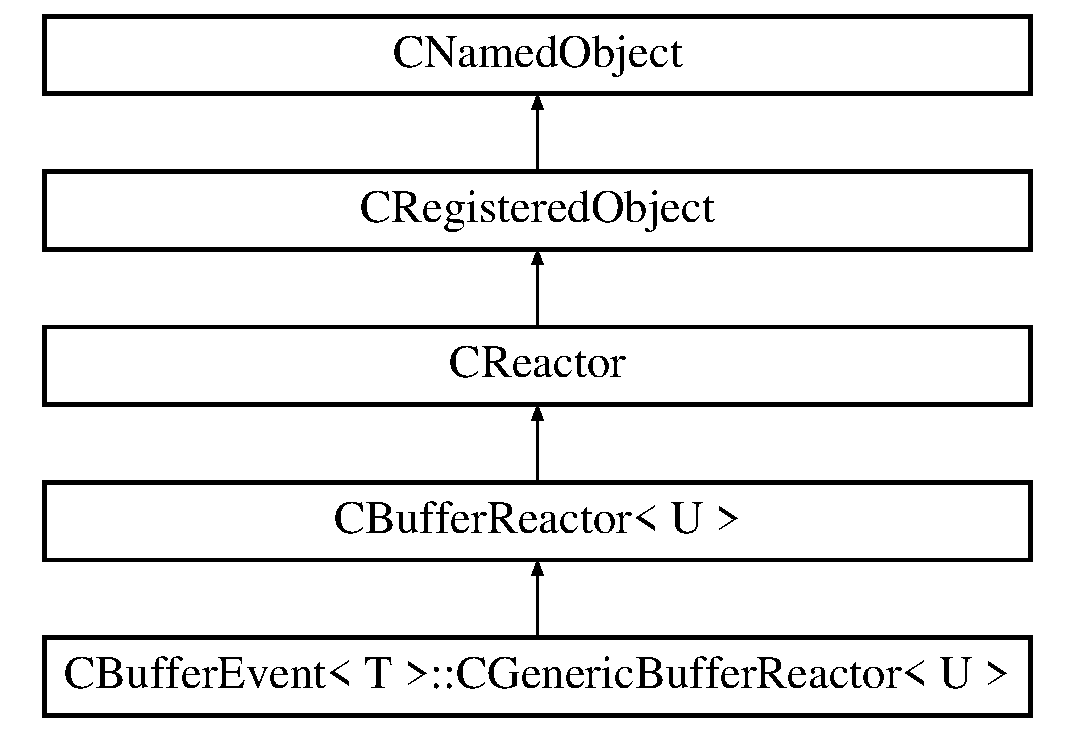
\includegraphics[height=5cm]{classCBufferEvent_1_1CGenericBufferReactor}
\end{center}
\end{figure}
\subsection*{Public Methods}
\begin{CompactItemize}
\item 
{\bf CGeneric\-Buffer\-Reactor} ({\bf CBuffer\-Event}$<$ U $>$ \&owner)
\item 
virtual void {\bf On\-Buffer} ({\bf CBuffer\-Monitor}$<$ T $>$ \&r\-Monitor, Pointer$<$ DAQBuffer$<$ T $>$, T $>$ p\-Buffer)
\item 
virtual void {\bf On\-Timeout} ({\bf CEvent\-Monitor} \&r\-Monitor)
\end{CompactItemize}
\subsection*{Private Attributes}
\begin{CompactItemize}
\item 
{\bf CBuffer\-Event}$<$ U $>$ \& {\bf m\_\-r\-Owner}
\end{CompactItemize}


\subsection{Detailed Description}
\subsubsection*{template$<$class T$>$template$<$class U$>$ class CBuffer\-Event$<$ T $>$::CGeneric\-Buffer\-Reactor$<$ U $>$}

The buffer reactor for {\bf CBuffer\-Event} {\rm (p.\,\pageref{classCBufferEvent})} is actually a nested class: It relays all of the calls back to the event's virtual functions. this allows the presentation of a monolithic model for managing the  events. 



Definition at line 360 of file CBuffer\-Event.h.

\subsection{Constructor \& Destructor Documentation}
\index{CBufferEvent::CGenericBufferReactor@{CBuffer\-Event::CGeneric\-Buffer\-Reactor}!CGenericBufferReactor@{CGenericBufferReactor}}
\index{CGenericBufferReactor@{CGenericBufferReactor}!CBufferEvent::CGenericBufferReactor@{CBuffer\-Event::CGeneric\-Buffer\-Reactor}}
\subsubsection{\setlength{\rightskip}{0pt plus 5cm}template$<$class T$>$ template$<$class U$>$ {\bf CBuffer\-Event}$<$ T $>$::CGeneric\-Buffer\-Reactor$<$ U $>$::CGeneric\-Buffer\-Reactor$<$ U $>$ ({\bf CBuffer\-Event}$<$ U $>$ \& {\em Owner})}\label{classCBufferEvent_1_1CGenericBufferReactor_a0}


Construct a Generic Buffer Reactor. This is the sort of buffer reactor which is associated with a {\bf CBuffer\-Event} {\rm (p.\,\pageref{classCBufferEvent})}. \begin{Desc}
\item[Parameters: ]\par
\begin{description}
\item[{\em 
Owner}]- Owning event. \end{description}
\end{Desc}


\subsection{Member Function Documentation}
\index{CBufferEvent::CGenericBufferReactor@{CBuffer\-Event::CGeneric\-Buffer\-Reactor}!OnBuffer@{OnBuffer}}
\index{OnBuffer@{OnBuffer}!CBufferEvent::CGenericBufferReactor@{CBuffer\-Event::CGeneric\-Buffer\-Reactor}}
\subsubsection{\setlength{\rightskip}{0pt plus 5cm}template$<$class T$>$ template$<$class U$>$ void {\bf CBuffer\-Event}$<$ T $>$::CGeneric\-Buffer\-Reactor$<$ U $>$::On\-Buffer ({\bf CBuffer\-Monitor}$<$ T $>$ \& {\em r\-MOnitor}, Pointer$<$ DAQBuffer$<$ T $>$, T $>$ {\em p\-Buffer})\hspace{0.3cm}{\tt  [virtual]}}\label{classCBufferEvent_1_1CGenericBufferReactor_a1}


Called when a buffer arrives. The Event's On\-Buffer is called with the pointer to the buffer.\begin{Desc}
\item[Parameters: ]\par
\begin{description}
\item[{\em 
r\-Monitor}]- reference to the monitor which fired the event. \item[{\em 
p\-Buffer}]- `Pointer' to the event buffer. \end{description}
\end{Desc}


Definition at line 327 of file CBuffer\-Event.cpp.

References CBuffer\-Event$<$ T $>$::CGeneric\-Buffer\-Reactor$<$ U $>$::m\_\-r\-Owner, and CBuffer\-Event$<$ U $>$::On\-Buffer().\index{CBufferEvent::CGenericBufferReactor@{CBuffer\-Event::CGeneric\-Buffer\-Reactor}!OnTimeout@{OnTimeout}}
\index{OnTimeout@{OnTimeout}!CBufferEvent::CGenericBufferReactor@{CBuffer\-Event::CGeneric\-Buffer\-Reactor}}
\subsubsection{\setlength{\rightskip}{0pt plus 5cm}template$<$class T$>$ template$<$class U$>$ void {\bf CBuffer\-Event}$<$ T $>$::CGeneric\-Buffer\-Reactor$<$ U $>$::On\-Timeout ({\bf CEvent\-Monitor} \& {\em r\-Monitor})\hspace{0.3cm}{\tt  [virtual]}}\label{classCBufferEvent_1_1CGenericBufferReactor_a2}


Called when the buffer monitor times out, but only if the buffer event has been programmed to pass timeouts on to user code. Again, this call is relayed to the Event's On\-Timeout function. \begin{Desc}
\item[Parameters: ]\par
\begin{description}
\item[{\em 
r\-Monitor}]- Reference to the event monitor (unused). \end{description}
\end{Desc}


Reimplemented from {\bf CReactor} {\rm (p.\,\pageref{classCReactor_a8})}.

Definition at line 344 of file CBuffer\-Event.cpp.

References CBuffer\-Event$<$ T $>$::CGeneric\-Buffer\-Reactor$<$ U $>$::m\_\-r\-Owner, and CBuffer\-Event$<$ U $>$::On\-Timeout().

\subsection{Member Data Documentation}
\index{CBufferEvent::CGenericBufferReactor@{CBuffer\-Event::CGeneric\-Buffer\-Reactor}!m_rOwner@{m\_\-rOwner}}
\index{m_rOwner@{m\_\-rOwner}!CBufferEvent::CGenericBufferReactor@{CBuffer\-Event::CGeneric\-Buffer\-Reactor}}
\subsubsection{\setlength{\rightskip}{0pt plus 5cm}template$<$class T$>$ template$<$class U$>$ {\bf CBuffer\-Event}$<$U$>$\& {\bf CBuffer\-Event}$<$ T $>$::CGeneric\-Buffer\-Reactor$<$ U $>$::m\_\-r\-Owner\hspace{0.3cm}{\tt  [private]}}\label{classCBufferEvent_1_1CGenericBufferReactor_o0}




Definition at line 362 of file CBuffer\-Event.h.

Referenced by CBuffer\-Event$<$ T $>$::CGeneric\-Buffer\-Reactor$<$ U $>$::On\-Buffer(), and CBuffer\-Event$<$ T $>$::CGeneric\-Buffer\-Reactor$<$ U $>$::On\-Timeout().

The documentation for this class was generated from the following files:\begin{CompactItemize}
\item 
{\bf CBuffer\-Event.h}\item 
{\bf CBuffer\-Event.cpp}\end{CompactItemize}

\section{CBuffer\-Monitor$<$ T $>$  Class Template Reference}
\label{classCBufferMonitor}\index{CBufferMonitor@{CBuffer\-Monitor}}
{\tt \#include $<$CBuffer\-Monitor.h$>$}

Inheritance diagram for CBuffer\-Monitor$<$ T $>$::\begin{figure}[H]
\begin{center}
\leavevmode
\includegraphics[height=4cm]{classCBufferMonitor}
\end{center}
\end{figure}
\subsection*{Public Methods}
\begin{CompactItemize}
\item 
{\bf CBuffer\-Monitor} (bool am\_\-f\-Timed\-Wait=true)
\item 
{\bf CBuffer\-Monitor} (const string \&r\-Name, bool am\_\-f\-Timed\-Wait=true)
\item 
{\bf CBuffer\-Monitor} (const char $\ast$p\-Name, bool am\_\-f\-Timed\-Wait=true)
\item 
{\bf $\sim$CBuffer\-Monitor} ()
\item 
DAQBuffer$<$ T $>$ \& {\bf get\-Buffer} ()
\item 
list$<$ {\bf Link\-Info} $>$ {\bf get\-Links} () const
\item 
DAQLink\-Mgr {\bf get\-Link\-Mgr} () const
\item 
virtual {\bf CEvent\-Monitor::result} {\bf operator()} ()
\item 
virtual int {\bf Add\-Link} (const string \&URL, int tag={\bf COS\_\-MAXBUFTAG}, int mask={\bf COS\_\-ALLBITS}, bool f\-Reliable=true)
\item 
void {\bf Remove\-Link} (int linkid)
\item 
void {\bf Remove\-Link} ({\bf Link\-Iterator} link)
\item 
template$<$typename Link\-Match\-Predicate$>$ {\bf Link\-Iterator} {\bf Find\-Link} (Link\-Match\-Predicate \&r\-Predicate, {\bf Link\-Iterator} startat)
\item 
{\bf Link\-Iterator} {\bf begin\-Links} ()
\item 
{\bf Link\-Iterator} {\bf end\-Links} ()
\item 
Pointer$<$ DAQBuffer$<$ T $>$, T $>$ {\bf get\-Buffer\-Pointer} (int n\-Offset=0)
\item 
void {\bf Set\-Buffer\-Tag} (int tag={\bf COS\_\-ALLBITS})
\item 
void {\bf Set\-Buffer\-Mask} (int n\-Mask)
\item 
string {\bf Describe\-Self} ()
\end{CompactItemize}
\subsection*{Protected Methods}
\begin{CompactItemize}
\item 
void {\bf set\-Buffer} (const DAQBuffer$<$ T $>$ am\_\-Buffer)
\item 
void {\bf set\-Links} (const list$<$ {\bf Link\-Info} $>$ am\_\-l\-Links)
\item 
void {\bf set\-Link\-Mgr} (const DAQLink\-Mgr am\_\-daq\_\-link\_\-mgr)
\end{CompactItemize}
\subsection*{Private Methods}
\begin{CompactItemize}
\item 
{\bf CBuffer\-Monitor} (const CBuffer\-Monitor$<$ T $>$ \&a\-CBuffer\-Monitor)
\item 
CBuffer\-Monitor$<$ T $>$ {\bf operator=} (const CBuffer\-Monitor$<$ T $>$ \&a\-CBuffer\-Monitor)
\end{CompactItemize}
\subsection*{Private Attributes}
\begin{CompactItemize}
\item 
DAQBuffer$<$ T $>$ {\bf m\_\-Buffer}
\item 
list$<$ {\bf Link\-Info} $>$ {\bf m\_\-l\-Links}
\item 
DAQLink\-Mgr {\bf daq\_\-link\_\-mgr}
\item 
int {\bf m\_\-n\-Tag}
\item 
int {\bf m\_\-n\-Mask}
\end{CompactItemize}
\subsubsection*{template$<$class T$>$ class CBuffer\-Monitor$<$ T $>$}



\subsection{Constructor \& Destructor Documentation}
\index{CBufferMonitor@{CBuffer\-Monitor}!CBufferMonitor@{CBufferMonitor}}
\index{CBufferMonitor@{CBufferMonitor}!CBufferMonitor@{CBuffer\-Monitor}}
\subsubsection{\setlength{\rightskip}{0pt plus 5cm}template$<$class T$>$ CBuffer\-Monitor$<$ T $>$::CBuffer\-Monitor (bool {\em am\_\-f\-Timed\-Wait} = true)\hspace{0.3cm}{\tt  [inline]}}\label{classCBufferMonitor_a0}


\index{CBufferMonitor@{CBuffer\-Monitor}!CBufferMonitor@{CBufferMonitor}}
\index{CBufferMonitor@{CBufferMonitor}!CBufferMonitor@{CBuffer\-Monitor}}
\subsubsection{\setlength{\rightskip}{0pt plus 5cm}template$<$class T$>$ CBuffer\-Monitor$<$ T $>$::CBuffer\-Monitor (const string \& {\em r\-Name}, bool {\em am\_\-f\-Timed\-Wait} = true)\hspace{0.3cm}{\tt  [inline]}}\label{classCBufferMonitor_a1}


\index{CBufferMonitor@{CBuffer\-Monitor}!CBufferMonitor@{CBufferMonitor}}
\index{CBufferMonitor@{CBufferMonitor}!CBufferMonitor@{CBuffer\-Monitor}}
\subsubsection{\setlength{\rightskip}{0pt plus 5cm}template$<$class T$>$ CBuffer\-Monitor$<$ T $>$::CBuffer\-Monitor (const char $\ast$ {\em p\-Name}, bool {\em am\_\-f\-Timed\-Wait} = true)\hspace{0.3cm}{\tt  [inline]}}\label{classCBufferMonitor_a2}


\index{CBufferMonitor@{CBuffer\-Monitor}!~CBufferMonitor@{$\sim$CBufferMonitor}}
\index{~CBufferMonitor@{$\sim$CBufferMonitor}!CBufferMonitor@{CBuffer\-Monitor}}
\subsubsection{\setlength{\rightskip}{0pt plus 5cm}template$<$class T$>$ CBuffer\-Monitor$<$ T $>$::$\sim$CBuffer\-Monitor ()\hspace{0.3cm}{\tt  [inline]}}\label{classCBufferMonitor_a3}


\index{CBufferMonitor@{CBuffer\-Monitor}!CBufferMonitor@{CBufferMonitor}}
\index{CBufferMonitor@{CBufferMonitor}!CBufferMonitor@{CBuffer\-Monitor}}
\subsubsection{\setlength{\rightskip}{0pt plus 5cm}template$<$class T$>$ CBuffer\-Monitor$<$ T $>$::CBuffer\-Monitor (const CBuffer\-Monitor$<$ T $>$ \& {\em a\-CBuffer\-Monitor})\hspace{0.3cm}{\tt  [private]}}\label{classCBufferMonitor_c0}




\subsection{Member Function Documentation}
\index{CBufferMonitor@{CBuffer\-Monitor}!AddLink@{AddLink}}
\index{AddLink@{AddLink}!CBufferMonitor@{CBuffer\-Monitor}}
\subsubsection{\setlength{\rightskip}{0pt plus 5cm}template$<$class T$>$ int CBuffer\-Monitor$<$ T $>$::Add\-Link (const string \& {\em URL}, int {\em tag} = {\bf COS\_\-MAXBUFTAG}, int {\em mask} = {\bf COS\_\-ALLBITS}, bool {\em f\-Reliable} = true)\hspace{0.3cm}{\tt  [virtual]}}\label{classCBufferMonitor_a8}


Operation Type: Mutator

Purpose: Adds a link to the link manager. The link id is returned. On failure, a {\bf CLink\-Failed\-Exception} {\rm (p.\,\pageref{classCLinkFailedException})} is thrown. 

Definition at line 337 of file CBuffer\-Monitor.cpp.

References CBuffer\-Monitor$<$ T $>$::daq\_\-link\_\-mgr, Link\-Info::linkid, CBuffer\-Monitor$<$ T $>$::m\_\-l\-Links, Link\-Info::Mask, Link\-Info::Tag, and Link\-Info::URL.\index{CBufferMonitor@{CBuffer\-Monitor}!beginLinks@{beginLinks}}
\index{beginLinks@{beginLinks}!CBufferMonitor@{CBuffer\-Monitor}}
\subsubsection{\setlength{\rightskip}{0pt plus 5cm}template$<$class T$>$ {\bf Link\-Iterator} CBuffer\-Monitor$<$ T $>$::begin\-Links ()}\label{classCBufferMonitor_a12}


Operation Type: Selector

Purpose: Returns an iterator to the beginning of the link list. 

Definition at line 458 of file CBuffer\-Monitor.cpp.

References CBuffer\-Monitor$<$ T $>$::m\_\-l\-Links.

Referenced by CBuffer\-Monitor$<$ T $>$::Describe\-Self().\index{CBufferMonitor@{CBuffer\-Monitor}!DescribeSelf@{DescribeSelf}}
\index{DescribeSelf@{DescribeSelf}!CBufferMonitor@{CBuffer\-Monitor}}
\subsubsection{\setlength{\rightskip}{0pt plus 5cm}template$<$class T$>$ string CBuffer\-Monitor$<$ T $>$::Describe\-Self ()\hspace{0.3cm}{\tt  [virtual]}}\label{classCBufferMonitor_a17}


Operation Type: Selector

Purpose: Produces a desciprtion string of the object. This includes 1. Calling CEvent\-Manager::Describe\-Self() 2. Putting out the tag and mask of the buffer. 3. Listing the links and their information. 

Reimplemented from {\bf CNamed\-Object} {\rm (p.\,\pageref{classCNamedObject_a8})}.

Definition at line 572 of file CBuffer\-Monitor.cpp.

References CBuffer\-Monitor$<$ T $>$::begin\-Links(), CNamed\-Object::Describe\-Self(), CBuffer\-Monitor$<$ T $>$::end\-Links(), Link\-Iterator, CBuffer\-Monitor$<$ T $>$::m\_\-Buffer, and CBuffer\-Monitor$<$ T $>$::m\_\-l\-Links.\index{CBufferMonitor@{CBuffer\-Monitor}!endLinks@{endLinks}}
\index{endLinks@{endLinks}!CBufferMonitor@{CBuffer\-Monitor}}
\subsubsection{\setlength{\rightskip}{0pt plus 5cm}template$<$class T$>$ {\bf Link\-Iterator} CBuffer\-Monitor$<$ T $>$::end\-Links ()}\label{classCBufferMonitor_a13}


Operation Type: Selector

Purpose: Returns an iterator suitable for determining end of iteration through the link list. 

Definition at line 475 of file CBuffer\-Monitor.cpp.

References CBuffer\-Monitor$<$ T $>$::m\_\-l\-Links.

Referenced by CBuffer\-Monitor$<$ T $>$::Describe\-Self().\index{CBufferMonitor@{CBuffer\-Monitor}!FindLink@{FindLink}}
\index{FindLink@{FindLink}!CBufferMonitor@{CBuffer\-Monitor}}
\subsubsection{\setlength{\rightskip}{0pt plus 5cm}template$<$class T$>$ template$<$class Link\-Match\-Predicate$>$ {\bf Link\-Iterator} CBuffer\-Monitor$<$ T $>$::Find\-Link (Link\-Match\-Predicate \& {\em r\-Predicate}, {\bf Link\-Iterator} {\em startat})}\label{classCBufferMonitor_a11}


Operation Type: Selector

Purpose: Locates the first link that satisfies a given predicate. Predefined predicates include: {\bf Match\-URL} {\rm (p.\,\pageref{classMatchURL})} - matches URL only {\bf Match\-All} {\rm (p.\,\pageref{classMatchAll})} - Matches URL, tag and mask. A Link\-Match\-Predicate is a function object implementing: bool operator()(Link\-Info) which returns TRUE if the link satisfies the predicate. Returns an iterator 'pointing' to the first match, or end() if there is no match. 

Definition at line 436 of file CBuffer\-Monitor.cpp.

References Link\-Iterator, and CBuffer\-Monitor$<$ T $>$::m\_\-l\-Links.\index{CBufferMonitor@{CBuffer\-Monitor}!getBuffer@{getBuffer}}
\index{getBuffer@{getBuffer}!CBufferMonitor@{CBuffer\-Monitor}}
\subsubsection{\setlength{\rightskip}{0pt plus 5cm}template$<$class T$>$ DAQBuffer$<$T$>$\& CBuffer\-Monitor$<$ T $>$::get\-Buffer ()\hspace{0.3cm}{\tt  [inline]}}\label{classCBufferMonitor_a4}




Definition at line 432 of file CBuffer\-Monitor.h.\index{CBufferMonitor@{CBuffer\-Monitor}!getBufferPointer@{getBufferPointer}}
\index{getBufferPointer@{getBufferPointer}!CBufferMonitor@{CBuffer\-Monitor}}
\subsubsection{\setlength{\rightskip}{0pt plus 5cm}template$<$class T$>$ Pointer$<$ DAQBuffer$<$ T $>$, T $>$ CBuffer\-Monitor$<$ T $>$::get\-Buffer\-Pointer (int {\em n\-Offset} = 0)}\label{classCBufferMonitor_a14}


Operation Type: Selector

Purpose: Returns a pointer to the DAQ Buffer. 

Definition at line 492 of file CBuffer\-Monitor.cpp.

References CBuffer\-Monitor$<$ T $>$::m\_\-Buffer.

Referenced by CBuffer\-Reactor$<$ T $>$::On\-Event().\index{CBufferMonitor@{CBuffer\-Monitor}!getLinkMgr@{getLinkMgr}}
\index{getLinkMgr@{getLinkMgr}!CBufferMonitor@{CBuffer\-Monitor}}
\subsubsection{\setlength{\rightskip}{0pt plus 5cm}template$<$class T$>$ DAQLink\-Mgr CBuffer\-Monitor$<$ T $>$::get\-Link\-Mgr () const\hspace{0.3cm}{\tt  [inline]}}\label{classCBufferMonitor_a6}




Definition at line 442 of file CBuffer\-Monitor.h.\index{CBufferMonitor@{CBuffer\-Monitor}!getLinks@{getLinks}}
\index{getLinks@{getLinks}!CBufferMonitor@{CBuffer\-Monitor}}
\subsubsection{\setlength{\rightskip}{0pt plus 5cm}template$<$class T$>$ list$<${\bf Link\-Info}$>$ CBuffer\-Monitor$<$ T $>$::get\-Links () const\hspace{0.3cm}{\tt  [inline]}}\label{classCBufferMonitor_a5}




Definition at line 437 of file CBuffer\-Monitor.h.\index{CBufferMonitor@{CBuffer\-Monitor}!operator()@{operator()}}
\index{operator()@{operator()}!CBufferMonitor@{CBuffer\-Monitor}}
\subsubsection{\setlength{\rightskip}{0pt plus 5cm}template$<$class T$>$ {\bf CEvent\-Monitor::result} CBuffer\-Monitor$<$ T $>$::operator() ()\hspace{0.3cm}{\tt  [virtual]}}\label{classCBufferMonitor_a7}


Operation Type: override

Purpose: Waits for a buffer to be received. Returns one of the following:  Occurred - a buffer was received into m\_\-Buffer Timed\-Out - Timeouts were enabled and no buffer was received during the timeout interval. 

Implements {\bf CEvent\-Monitor} {\rm (p.\,\pageref{classCEventMonitor_a7})}.

Definition at line 300 of file CBuffer\-Monitor.cpp.

References CEvent\-Monitor::get\-Timed\-Wait(), CEvent\-Monitor::get\-Timeout(), CBuffer\-Monitor$<$ T $>$::m\_\-Buffer, CBuffer\-Monitor$<$ T $>$::m\_\-n\-Mask, CBuffer\-Monitor$<$ T $>$::m\_\-n\-Tag, CEvent\-Monitor::Occurred, and CEvent\-Monitor::Timed\-Out.\index{CBufferMonitor@{CBuffer\-Monitor}!operator=@{operator=}}
\index{operator=@{operator=}!CBufferMonitor@{CBuffer\-Monitor}}
\subsubsection{\setlength{\rightskip}{0pt plus 5cm}template$<$class T$>$ CBuffer\-Monitor$<$T$>$ CBuffer\-Monitor$<$ T $>$::operator= (const CBuffer\-Monitor$<$ T $>$ \& {\em a\-CBuffer\-Monitor})\hspace{0.3cm}{\tt  [private]}}\label{classCBufferMonitor_c1}


\index{CBufferMonitor@{CBuffer\-Monitor}!RemoveLink@{RemoveLink}}
\index{RemoveLink@{RemoveLink}!CBufferMonitor@{CBuffer\-Monitor}}
\subsubsection{\setlength{\rightskip}{0pt plus 5cm}template$<$class T$>$ void CBuffer\-Monitor$<$ T $>$::Remove\-Link ({\bf Link\-Iterator} {\em link})}\label{classCBufferMonitor_a10}


Operation Type: Mutator

Purpose: Removes a link given the iterator to its link structure in the link list. If the iterator is end(), a {\bf CNo\-Such\-Link\-Exception} {\rm (p.\,\pageref{classCNoSuchLinkException})} is thrown. 

Definition at line 401 of file CBuffer\-Monitor.cpp.

References CBuffer\-Monitor$<$ T $>$::daq\_\-link\_\-mgr, Link\-Iterator, and CBuffer\-Monitor$<$ T $>$::m\_\-l\-Links.\index{CBufferMonitor@{CBuffer\-Monitor}!RemoveLink@{RemoveLink}}
\index{RemoveLink@{RemoveLink}!CBufferMonitor@{CBuffer\-Monitor}}
\subsubsection{\setlength{\rightskip}{0pt plus 5cm}template$<$class T$>$ void CBuffer\-Monitor$<$ T $>$::Remove\-Link (int {\em linkid})}\label{classCBufferMonitor_a9}


Operation Type: Mutator

Purpose: If the specified link exists, it is removed from the link list and deleted from the spectrodaq link manager. If the link does not exist, a {\bf CNo\-Such\-Link\-Exception} {\rm (p.\,\pageref{classCNoSuchLinkException})} is thrown. 

Definition at line 370 of file CBuffer\-Monitor.cpp.

References CBuffer\-Monitor$<$ T $>$::daq\_\-link\_\-mgr, Link\-Iterator, and CBuffer\-Monitor$<$ T $>$::m\_\-l\-Links.\index{CBufferMonitor@{CBuffer\-Monitor}!setBuffer@{setBuffer}}
\index{setBuffer@{setBuffer}!CBufferMonitor@{CBuffer\-Monitor}}
\subsubsection{\setlength{\rightskip}{0pt plus 5cm}template$<$class T$>$ void CBuffer\-Monitor$<$ T $>$::set\-Buffer (const DAQBuffer$<$ T $>$ {\em am\_\-Buffer})\hspace{0.3cm}{\tt  [inline, protected]}}\label{classCBufferMonitor_b0}




Definition at line 450 of file CBuffer\-Monitor.h.\index{CBufferMonitor@{CBuffer\-Monitor}!SetBufferMask@{SetBufferMask}}
\index{SetBufferMask@{SetBufferMask}!CBufferMonitor@{CBuffer\-Monitor}}
\subsubsection{\setlength{\rightskip}{0pt plus 5cm}template$<$class T$>$ void CBuffer\-Monitor$<$ T $>$::Set\-Buffer\-Mask (int {\em n\-Mask})}\label{classCBufferMonitor_a16}


Operation Type: Mutator

Purpose: Sets the receive mask associated with the buffer. See Set\-Buffer\-Tag for an explanation of tags and masks and how they interact with link tags and masks and the tag of the incomming buffer to determine receipt. 

Definition at line 547 of file CBuffer\-Monitor.cpp.

References CBuffer\-Monitor$<$ T $>$::m\_\-Buffer, and CBuffer\-Monitor$<$ T $>$::m\_\-n\-Mask.

Referenced by CBuffer\-Event$<$ U $>$::set\-Buffer\-Mask().\index{CBufferMonitor@{CBuffer\-Monitor}!SetBufferTag@{SetBufferTag}}
\index{SetBufferTag@{SetBufferTag}!CBufferMonitor@{CBuffer\-Monitor}}
\subsubsection{\setlength{\rightskip}{0pt plus 5cm}template$<$class T$>$ void CBuffer\-Monitor$<$ T $>$::Set\-Buffer\-Tag (int {\em tag} = {\bf COS\_\-ALLBITS})}\label{classCBufferMonitor_a15}


Operation Type: Mutator

Purpose: Sets the tag matched on receives into the buffer. For each link/buffer pair, tags are used to determine which buffers routed through Spectro\-Daq will be received by a link or buffer. The logic is that at each stage, the routed buffer's tag is anded with the receiving entity's mask. If this is equal to the receiving entity's tag, the buffer is accepted. So, for a given link (link.mask, link.tag), and our buffer (buffer.mask, buffer.tag): A routed buffer rbuffer.tag is received when:

((rbuffer.tag \& link.mask) == link.tag) \&\& ((rbuffer.tag \& buffer.mask) == buffer.tag) 

Definition at line 522 of file CBuffer\-Monitor.cpp.

References CBuffer\-Monitor$<$ T $>$::m\_\-Buffer, and CBuffer\-Monitor$<$ T $>$::m\_\-n\-Tag.

Referenced by CBuffer\-Event$<$ U $>$::set\-Buffer\-Tag().\index{CBufferMonitor@{CBuffer\-Monitor}!setLinkMgr@{setLinkMgr}}
\index{setLinkMgr@{setLinkMgr}!CBufferMonitor@{CBuffer\-Monitor}}
\subsubsection{\setlength{\rightskip}{0pt plus 5cm}template$<$class T$>$ void CBuffer\-Monitor$<$ T $>$::set\-Link\-Mgr (const DAQLink\-Mgr {\em am\_\-daq\_\-link\_\-mgr})\hspace{0.3cm}{\tt  [inline, protected]}}\label{classCBufferMonitor_b2}




Definition at line 460 of file CBuffer\-Monitor.h.\index{CBufferMonitor@{CBuffer\-Monitor}!setLinks@{setLinks}}
\index{setLinks@{setLinks}!CBufferMonitor@{CBuffer\-Monitor}}
\subsubsection{\setlength{\rightskip}{0pt plus 5cm}template$<$class T$>$ void CBuffer\-Monitor$<$ T $>$::set\-Links (const list$<$ {\bf Link\-Info} $>$ {\em am\_\-l\-Links})\hspace{0.3cm}{\tt  [inline, protected]}}\label{classCBufferMonitor_b1}




Definition at line 455 of file CBuffer\-Monitor.h.

\subsection{Member Data Documentation}
\index{CBufferMonitor@{CBuffer\-Monitor}!daq_link_mgr@{daq\_\-link\_\-mgr}}
\index{daq_link_mgr@{daq\_\-link\_\-mgr}!CBufferMonitor@{CBuffer\-Monitor}}
\subsubsection{\setlength{\rightskip}{0pt plus 5cm}template$<$class T$>$ DAQLink\-Mgr CBuffer\-Monitor$<$ T $>$::daq\_\-link\_\-mgr\hspace{0.3cm}{\tt  [private]}}\label{classCBufferMonitor_o2}


List of links. 

Definition at line 376 of file CBuffer\-Monitor.h.

Referenced by CBuffer\-Monitor$<$ T $>$::Add\-Link(), CBuffer\-Monitor$<$ U $>$::get\-Link\-Mgr(), CBuffer\-Monitor$<$ T $>$::Remove\-Link(), and CBuffer\-Monitor$<$ U $>$::set\-Link\-Mgr().\index{CBufferMonitor@{CBuffer\-Monitor}!m_Buffer@{m\_\-Buffer}}
\index{m_Buffer@{m\_\-Buffer}!CBufferMonitor@{CBuffer\-Monitor}}
\subsubsection{\setlength{\rightskip}{0pt plus 5cm}template$<$class T$>$ DAQBuffer$<$T$>$ CBuffer\-Monitor$<$ T $>$::m\_\-Buffer\hspace{0.3cm}{\tt  [private]}}\label{classCBufferMonitor_o0}




Definition at line 374 of file CBuffer\-Monitor.h.

Referenced by CBuffer\-Monitor$<$ T $>$::Describe\-Self(), CBuffer\-Monitor$<$ U $>$::get\-Buffer(), CBuffer\-Monitor$<$ T $>$::get\-Buffer\-Pointer(), CBuffer\-Monitor$<$ T $>$::operator()(), CBuffer\-Monitor$<$ U $>$::set\-Buffer(), CBuffer\-Monitor$<$ T $>$::Set\-Buffer\-Mask(), and CBuffer\-Monitor$<$ T $>$::Set\-Buffer\-Tag().\index{CBufferMonitor@{CBuffer\-Monitor}!m_lLinks@{m\_\-lLinks}}
\index{m_lLinks@{m\_\-lLinks}!CBufferMonitor@{CBuffer\-Monitor}}
\subsubsection{\setlength{\rightskip}{0pt plus 5cm}template$<$class T$>$ list$<${\bf Link\-Info}$>$ CBuffer\-Monitor$<$ T $>$::m\_\-l\-Links\hspace{0.3cm}{\tt  [private]}}\label{classCBufferMonitor_o1}


Encapsulated buffer 

Definition at line 375 of file CBuffer\-Monitor.h.

Referenced by CBuffer\-Monitor$<$ T $>$::Add\-Link(), CBuffer\-Monitor$<$ T $>$::begin\-Links(), CBuffer\-Monitor$<$ T $>$::Describe\-Self(), CBuffer\-Monitor$<$ T $>$::end\-Links(), CBuffer\-Monitor$<$ T $>$::Find\-Link(), CBuffer\-Monitor$<$ U $>$::get\-Links(), CBuffer\-Monitor$<$ T $>$::Remove\-Link(), and CBuffer\-Monitor$<$ U $>$::set\-Links().\index{CBufferMonitor@{CBuffer\-Monitor}!m_nMask@{m\_\-nMask}}
\index{m_nMask@{m\_\-nMask}!CBufferMonitor@{CBuffer\-Monitor}}
\subsubsection{\setlength{\rightskip}{0pt plus 5cm}template$<$class T$>$ int CBuffer\-Monitor$<$ T $>$::m\_\-n\-Mask\hspace{0.3cm}{\tt  [private]}}\label{classCBufferMonitor_o4}




Definition at line 378 of file CBuffer\-Monitor.h.

Referenced by CBuffer\-Monitor$<$ T $>$::operator()(), and CBuffer\-Monitor$<$ T $>$::Set\-Buffer\-Mask().\index{CBufferMonitor@{CBuffer\-Monitor}!m_nTag@{m\_\-nTag}}
\index{m_nTag@{m\_\-nTag}!CBufferMonitor@{CBuffer\-Monitor}}
\subsubsection{\setlength{\rightskip}{0pt plus 5cm}template$<$class T$>$ int CBuffer\-Monitor$<$ T $>$::m\_\-n\-Tag\hspace{0.3cm}{\tt  [private]}}\label{classCBufferMonitor_o3}


A link manager 

Definition at line 377 of file CBuffer\-Monitor.h.

Referenced by CBuffer\-Monitor$<$ T $>$::operator()(), and CBuffer\-Monitor$<$ T $>$::Set\-Buffer\-Tag().

The documentation for this class was generated from the following files:\begin{CompactItemize}
\item 
{\bf CBuffer\-Monitor.h}\item 
{\bf CBuffer\-Monitor.cpp}\end{CompactItemize}

\section{CBuffer\-Reactor$<$ T $>$  Class Template Reference}
\label{classCBufferReactor}\index{CBufferReactor@{CBuffer\-Reactor}}
{\tt \#include $<$CBuffer\-Reactor.h$>$}

Inheritance diagram for CBuffer\-Reactor$<$ T $>$::\begin{figure}[H]
\begin{center}
\leavevmode
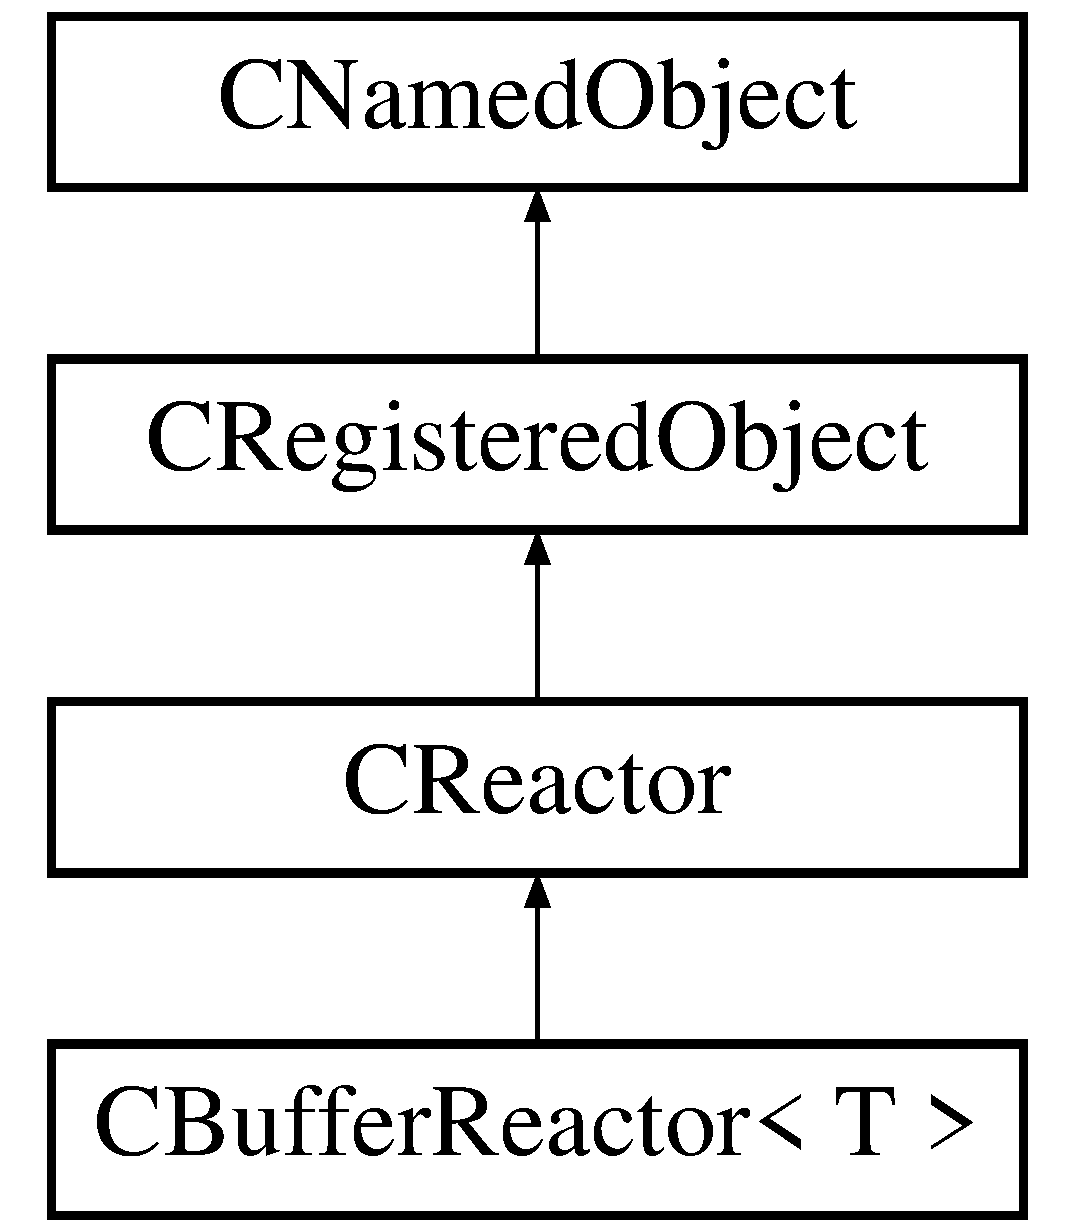
\includegraphics[height=4cm]{classCBufferReactor}
\end{center}
\end{figure}
\subsection*{Public Methods}
\begin{CompactItemize}
\item 
{\bf CBuffer\-Reactor} ()
\item 
{\bf CBuffer\-Reactor} (const string \&r\-Name)
\item 
{\bf CBuffer\-Reactor} (const char $\ast$p\-Name)
\item 
{\bf $\sim$CBuffer\-Reactor} ()
\item 
template$<$class U$>$ int {\bf operator==} (const CBuffer\-Reactor$<$ U $>$ \&a\-CBuffer\-Reactor) const
\begin{CompactList}\small\item\em Operator== Equality comparison:.\item\end{CompactList}\item 
virtual void {\bf On\-Event} ({\bf CEvent\-Monitor} \&r\-Monitor)
\item 
virtual void {\bf On\-Buffer} ({\bf CBuffer\-Monitor}$<$ T $>$ \&r\-Monitor, Pointer$<$ DAQBuffer$<$ T $>$, T $>$ p\-Buffer)
\end{CompactItemize}
\subsection*{Private Methods}
\begin{CompactItemize}
\item 
{\bf CBuffer\-Reactor} (const CBuffer\-Reactor \&a\-CBuffer\-Reactor)
\begin{CompactList}\small\item\em Copy Constructor disallowed.\item\end{CompactList}\item 
CBuffer\-Reactor \& {\bf operator=} (const CBuffer\-Reactor \&a\-CBuffer\-Reactor)
\begin{CompactList}\small\item\em Operator= Assignment Operator disallowed.\item\end{CompactList}\end{CompactItemize}


\subsection{Detailed Description}
\subsubsection*{template$<$class T$>$ class CBuffer\-Reactor$<$ T $>$}

Base class for Spectro\-Daq buffer receipt. This object must be subclassed to provide application specific processing. 



Definition at line 327 of file CBuffer\-Reactor.h.

\subsection{Constructor \& Destructor Documentation}
\index{CBufferReactor@{CBuffer\-Reactor}!CBufferReactor@{CBufferReactor}}
\index{CBufferReactor@{CBufferReactor}!CBufferReactor@{CBuffer\-Reactor}}
\subsubsection{\setlength{\rightskip}{0pt plus 5cm}template$<$class T$>$ CBuffer\-Reactor$<$ T $>$::CBuffer\-Reactor ()}\label{classCBufferReactor_a0}


Construct a buffer reactor with a default name. Note that buffer reactors are templated by the type of data contained in the buffer. 

Definition at line 310 of file CBuffer\-Reactor.cpp.

References CNamed\-Object::Append\-Class\-Info().\index{CBufferReactor@{CBuffer\-Reactor}!CBufferReactor@{CBufferReactor}}
\index{CBufferReactor@{CBufferReactor}!CBufferReactor@{CBuffer\-Reactor}}
\subsubsection{\setlength{\rightskip}{0pt plus 5cm}template$<$class T$>$ CBuffer\-Reactor$<$ T $>$::CBuffer\-Reactor (const string \& {\em r\-Name})}\label{classCBufferReactor_a1}


Construct a named buffer reactor using an STL string parameter for the object name. \begin{Desc}
\item[Parameters: ]\par
\begin{description}
\item[{\em 
r\-Name}]- the name of the reactor. \end{description}
\end{Desc}


Definition at line 322 of file CBuffer\-Reactor.cpp.

References CNamed\-Object::Append\-Class\-Info().\index{CBufferReactor@{CBuffer\-Reactor}!CBufferReactor@{CBufferReactor}}
\index{CBufferReactor@{CBufferReactor}!CBufferReactor@{CBuffer\-Reactor}}
\subsubsection{\setlength{\rightskip}{0pt plus 5cm}template$<$class T$>$ CBuffer\-Reactor$<$ T $>$::CBuffer\-Reactor (const char $\ast$ {\em p\-Name})}\label{classCBufferReactor_a2}


Construct a named buffer reactor using a ASCIZ (C) string parameter for the object name. \begin{Desc}
\item[Parameters: ]\par
\begin{description}
\item[{\em 
p\-Name}]- Pointer to an ASCIZ string naming the buffer. \end{description}
\end{Desc}


Definition at line 334 of file CBuffer\-Reactor.cpp.

References CNamed\-Object::Append\-Class\-Info().\index{CBufferReactor@{CBuffer\-Reactor}!~CBufferReactor@{$\sim$CBufferReactor}}
\index{~CBufferReactor@{$\sim$CBufferReactor}!CBufferReactor@{CBuffer\-Reactor}}
\subsubsection{\setlength{\rightskip}{0pt plus 5cm}template$<$class T$>$ CBuffer\-Reactor$<$ T $>$::$\sim$CBuffer\-Reactor ()}\label{classCBufferReactor_a3}




Definition at line 340 of file CBuffer\-Reactor.cpp.\index{CBufferReactor@{CBuffer\-Reactor}!CBufferReactor@{CBufferReactor}}
\index{CBufferReactor@{CBufferReactor}!CBufferReactor@{CBuffer\-Reactor}}
\subsubsection{\setlength{\rightskip}{0pt plus 5cm}template$<$class T$>$ CBuffer\-Reactor$<$ T $>$::CBuffer\-Reactor (const CBuffer\-Reactor$<$ T $>$ \& {\em a\-CBuffer\-Reactor})\hspace{0.3cm}{\tt  [private]}}\label{classCBufferReactor_c0}


Copy Constructor disallowed.



\subsection{Member Function Documentation}
\index{CBufferReactor@{CBuffer\-Reactor}!OnBuffer@{OnBuffer}}
\index{OnBuffer@{OnBuffer}!CBufferReactor@{CBuffer\-Reactor}}
\subsubsection{\setlength{\rightskip}{0pt plus 5cm}template$<$class T$>$ void CBuffer\-Reactor$<$ T $>$::On\-Buffer ({\bf CBuffer\-Monitor}$<$ T $>$ \& {\em r\-Monitor}, Pointer$<$ DAQBuffer$<$ T $>$, T $>$ {\em p\-Buffer})\hspace{0.3cm}{\tt  [virtual]}}\label{classCBufferReactor_a6}


Called when a buffer has been received by a buffer monitor. In normal use, the user will subclass CBuffer\-Reactor and override this no-op member. \begin{Desc}
\item[Parameters: ]\par
\begin{description}
\item[{\em 
r\-Monitor}]- The buffer monitor which received the buffer. \item[{\em 
p\-Buffer}]- A DAQBuffer\-Ptr of the appropriate type into the buffer received. \end{description}
\end{Desc}


Reimplemented in {\bf CBuffer\-Event$<$ T $>$::CGeneric\-Buffer\-Reactor$<$ T $>$} {\rm (p.\,\pageref{classCBufferEvent_1_1CGenericBufferReactor_a1})}.

Definition at line 389 of file CBuffer\-Reactor.cpp.

Referenced by CBuffer\-Reactor$<$ T $>$::On\-Event().\index{CBufferReactor@{CBuffer\-Reactor}!OnEvent@{OnEvent}}
\index{OnEvent@{OnEvent}!CBufferReactor@{CBuffer\-Reactor}}
\subsubsection{\setlength{\rightskip}{0pt plus 5cm}template$<$class T$>$ void CBuffer\-Reactor$<$ T $>$::On\-Event ({\bf CEvent\-Monitor} \& {\em r\-Monitor})\hspace{0.3cm}{\tt  [virtual]}}\label{classCBufferReactor_a5}


Called when the event monitor declares an event. The event monitor must be descended from {\bf CBuffer\-Monitor} {\rm (p.\,\pageref{classCBufferMonitor})} or  this function will throw a {\bf CIncompatible\-Monitor} {\rm (p.\,\pageref{classCIncompatibleMonitor})} exception. The On\-Buffer virtual member is called with a pointer to the buffer. \begin{Desc}
\item[Parameters: ]\par
\begin{description}
\item[{\em 
r\-Monitor}]- Reference to the monitor which declared the event. \end{description}
\end{Desc}


Reimplemented from {\bf CReactor} {\rm (p.\,\pageref{classCReactor_a6})}.

Definition at line 365 of file CBuffer\-Reactor.cpp.

References CBuffer\-Monitor$<$ T $>$::get\-Buffer\-Pointer(), and CBuffer\-Reactor$<$ T $>$::On\-Buffer().\index{CBufferReactor@{CBuffer\-Reactor}!operator=@{operator=}}
\index{operator=@{operator=}!CBufferReactor@{CBuffer\-Reactor}}
\subsubsection{\setlength{\rightskip}{0pt plus 5cm}template$<$class T$>$ CBuffer\-Reactor\& CBuffer\-Reactor$<$ T $>$::operator= (const CBuffer\-Reactor$<$ T $>$ \& {\em a\-CBuffer\-Reactor})\hspace{0.3cm}{\tt  [private]}}\label{classCBufferReactor_c1}


Operator= Assignment Operator disallowed.

\index{CBufferReactor@{CBuffer\-Reactor}!operator==@{operator==}}
\index{operator==@{operator==}!CBufferReactor@{CBuffer\-Reactor}}
\subsubsection{\setlength{\rightskip}{0pt plus 5cm}template$<$class T$>$ template$<$class U$>$ int CBuffer\-Reactor$<$ T $>$::operator== (const CBuffer\-Reactor$<$ U $>$ \& {\em a\-CBuffer\-Reactor}) const}\label{classCBufferReactor_a4}


Operator== Equality comparison:.



Definition at line 349 of file CBuffer\-Reactor.cpp.

References CReactor::operator==().

The documentation for this class was generated from the following files:\begin{CompactItemize}
\item 
{\bf CBuffer\-Reactor.h}\item 
{\bf CBuffer\-Reactor.cpp}\end{CompactItemize}

\section{CChanged\-Predicate$<$ T $>$  Class Template Reference}
\label{classCChangedPredicate}\index{CChangedPredicate@{CChanged\-Predicate}}
{\tt \#include $<$CChanged\-Predicate.h$>$}

Inheritance diagram for CChanged\-Predicate$<$ T $>$::\begin{figure}[H]
\begin{center}
\leavevmode
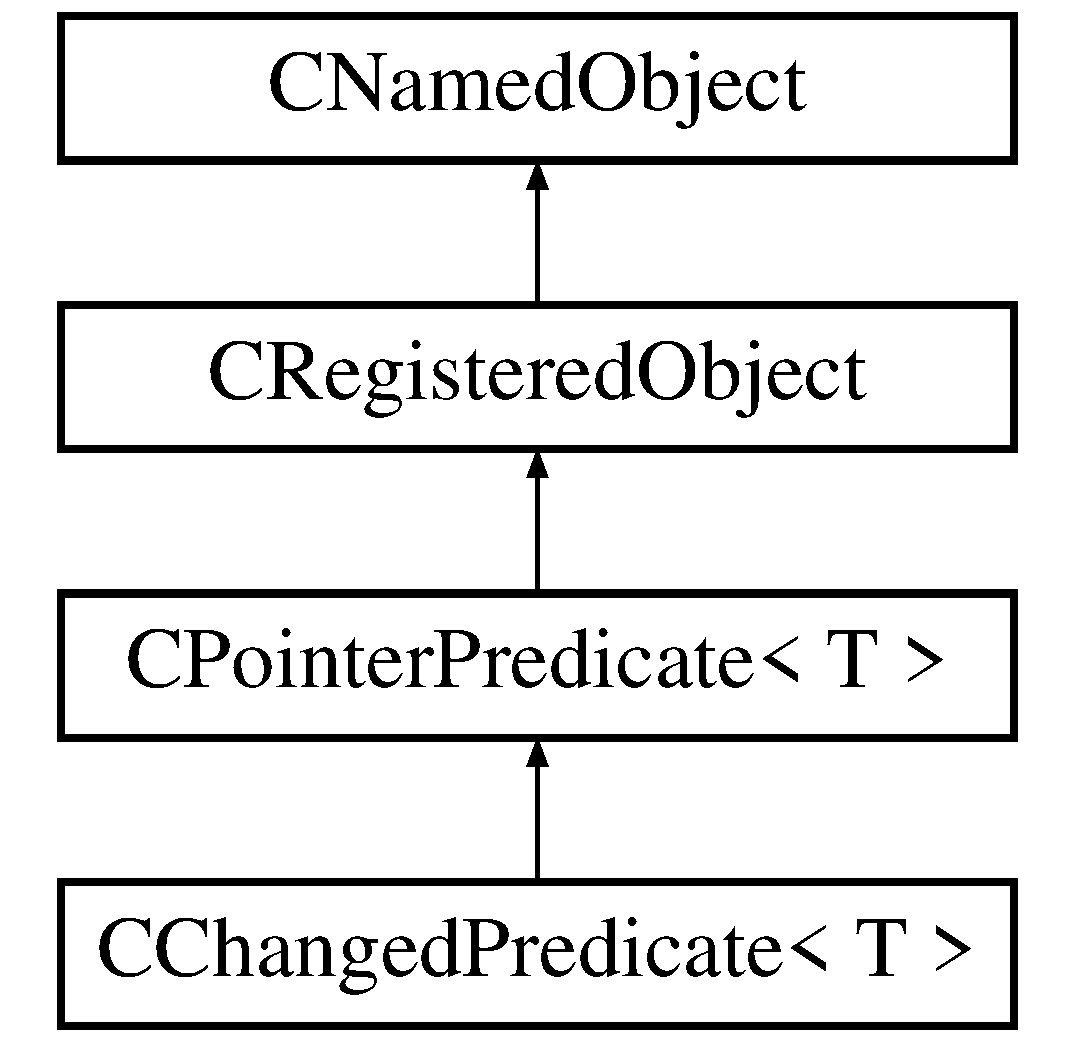
\includegraphics[height=4cm]{classCChangedPredicate}
\end{center}
\end{figure}
\subsection*{Public Methods}
\begin{CompactItemize}
\item 
{\bf CChanged\-Predicate} (T am\_\-TOld\-Value)
\item 
{\bf CChanged\-Predicate} (const string \&r\-Name, T am\_\-TOld\-Value)
\item 
{\bf CChanged\-Predicate} (const char $\ast$p\-Name, T am\_\-TOld\-Value)
\item 
{\bf $\sim$CChanged\-Predicate} ()
\item 
int {\bf operator==} (const CChanged\-Predicate$<$ T $>$ \&a\-CChanged\-Predicate) const
\item 
T {\bf get\-Old\-Value} () const
\item 
virtual bool {\bf operator()} (T n\-Value)
\item 
virtual string {\bf Describe\-Self} ()
\end{CompactItemize}
\subsection*{Protected Methods}
\begin{CompactItemize}
\item 
void {\bf set\-Old\-Value} (const T am\_\-TOld\-Value)
\end{CompactItemize}
\subsection*{Private Methods}
\begin{CompactItemize}
\item 
{\bf CChanged\-Predicate} (const CChanged\-Predicate$<$ T $>$ \&a\-CChanged\-Predicate)
\item 
CChanged\-Predicate$<$ T $>$ {\bf operator=} (const CChanged\-Predicate$<$ T $>$ \&a\-CChanged\-Predicate)
\end{CompactItemize}
\subsection*{Private Attributes}
\begin{CompactItemize}
\item 
T {\bf m\_\-TOld\-Value}
\end{CompactItemize}


\subsection{Detailed Description}
\subsubsection*{template$<$typename T$>$ class CChanged\-Predicate$<$ T $>$}

$\backslash$class: CChanged\-Predicate

Defines a pointer predicate which is satisfied whenever the current value changes.

Author: Jason Venema NSCL Michigan State University East Lansing, MI 48824-1321 mailto: {\tt venemaja@msu.edu} 



Definition at line 301 of file CChanged\-Predicate.h.

\subsection{Constructor \& Destructor Documentation}
\index{CChangedPredicate@{CChanged\-Predicate}!CChangedPredicate@{CChangedPredicate}}
\index{CChangedPredicate@{CChangedPredicate}!CChangedPredicate@{CChanged\-Predicate}}
\subsubsection{\setlength{\rightskip}{0pt plus 5cm}template$<$typename T$>$ CChanged\-Predicate$<$ T $>$::CChanged\-Predicate (T {\em am\_\-TOld\-Value})\hspace{0.3cm}{\tt  [inline]}}\label{classCChangedPredicate_a0}


Prior value \index{CChangedPredicate@{CChanged\-Predicate}!CChangedPredicate@{CChangedPredicate}}
\index{CChangedPredicate@{CChangedPredicate}!CChangedPredicate@{CChanged\-Predicate}}
\subsubsection{\setlength{\rightskip}{0pt plus 5cm}template$<$typename T$>$ CChanged\-Predicate$<$ T $>$::CChanged\-Predicate (const string \& {\em r\-Name}, T {\em am\_\-TOld\-Value})\hspace{0.3cm}{\tt  [inline]}}\label{classCChangedPredicate_a1}


\index{CChangedPredicate@{CChanged\-Predicate}!CChangedPredicate@{CChangedPredicate}}
\index{CChangedPredicate@{CChangedPredicate}!CChangedPredicate@{CChanged\-Predicate}}
\subsubsection{\setlength{\rightskip}{0pt plus 5cm}template$<$typename T$>$ CChanged\-Predicate$<$ T $>$::CChanged\-Predicate (const char $\ast$ {\em p\-Name}, T {\em am\_\-TOld\-Value})\hspace{0.3cm}{\tt  [inline]}}\label{classCChangedPredicate_a2}


\index{CChangedPredicate@{CChanged\-Predicate}!~CChangedPredicate@{$\sim$CChangedPredicate}}
\index{~CChangedPredicate@{$\sim$CChangedPredicate}!CChangedPredicate@{CChanged\-Predicate}}
\subsubsection{\setlength{\rightskip}{0pt plus 5cm}template$<$typename T$>$ CChanged\-Predicate$<$ T $>$::$\sim$CChanged\-Predicate ()\hspace{0.3cm}{\tt  [inline]}}\label{classCChangedPredicate_a3}


\index{CChangedPredicate@{CChanged\-Predicate}!CChangedPredicate@{CChangedPredicate}}
\index{CChangedPredicate@{CChangedPredicate}!CChangedPredicate@{CChanged\-Predicate}}
\subsubsection{\setlength{\rightskip}{0pt plus 5cm}template$<$typename T$>$ CChanged\-Predicate$<$ T $>$::CChanged\-Predicate (const CChanged\-Predicate$<$ T $>$ \& {\em a\-CChanged\-Predicate})\hspace{0.3cm}{\tt  [private]}}\label{classCChangedPredicate_c0}




\subsection{Member Function Documentation}
\index{CChangedPredicate@{CChanged\-Predicate}!DescribeSelf@{DescribeSelf}}
\index{DescribeSelf@{DescribeSelf}!CChangedPredicate@{CChanged\-Predicate}}
\subsubsection{\setlength{\rightskip}{0pt plus 5cm}template$<$typename T$>$ string CChanged\-Predicate$<$ T $>$::Describe\-Self ()\hspace{0.3cm}{\tt  [virtual]}}\label{classCChangedPredicate_a7}


Describes the named object. The information given is the object type given by m\_\-s\-Class\-Path, and the object name. 

Implements {\bf CPointer\-Predicate$<$ T $>$} {\rm (p.\,\pageref{classCPointerPredicate_a6})}.

Definition at line 319 of file CChanged\-Predicate.cpp.

References CChanged\-Predicate$<$ T $>$::m\_\-TOld\-Value.\index{CChangedPredicate@{CChanged\-Predicate}!getOldValue@{getOldValue}}
\index{getOldValue@{getOldValue}!CChangedPredicate@{CChanged\-Predicate}}
\subsubsection{\setlength{\rightskip}{0pt plus 5cm}template$<$typename T$>$ T CChanged\-Predicate$<$ T $>$::get\-Old\-Value () const\hspace{0.3cm}{\tt  [inline]}}\label{classCChangedPredicate_a5}




Definition at line 344 of file CChanged\-Predicate.h.\index{CChangedPredicate@{CChanged\-Predicate}!operator()@{operator()}}
\index{operator()@{operator()}!CChangedPredicate@{CChanged\-Predicate}}
\subsubsection{\setlength{\rightskip}{0pt plus 5cm}template$<$typename T$>$ bool CChanged\-Predicate$<$ T $>$::operator() (T {\em n\-Value})\hspace{0.3cm}{\tt  [virtual]}}\label{classCChangedPredicate_a6}




Implements {\bf CPointer\-Predicate$<$ T $>$} {\rm (p.\,\pageref{classCPointerPredicate_a5})}.

Definition at line 300 of file CChanged\-Predicate.cpp.

References CChanged\-Predicate$<$ T $>$::m\_\-TOld\-Value.\index{CChangedPredicate@{CChanged\-Predicate}!operator=@{operator=}}
\index{operator=@{operator=}!CChangedPredicate@{CChanged\-Predicate}}
\subsubsection{\setlength{\rightskip}{0pt plus 5cm}template$<$typename T$>$ CChanged\-Predicate$<$T$>$ CChanged\-Predicate$<$ T $>$::operator= (const CChanged\-Predicate$<$ T $>$ \& {\em a\-CChanged\-Predicate})\hspace{0.3cm}{\tt  [private]}}\label{classCChangedPredicate_c1}


\index{CChangedPredicate@{CChanged\-Predicate}!operator==@{operator==}}
\index{operator==@{operator==}!CChangedPredicate@{CChanged\-Predicate}}
\subsubsection{\setlength{\rightskip}{0pt plus 5cm}template$<$typename T$>$ int CChanged\-Predicate$<$ T $>$::operator== (const CChanged\-Predicate$<$ T $>$ \& {\em a\-CChanged\-Predicate}) const\hspace{0.3cm}{\tt  [inline]}}\label{classCChangedPredicate_a4}




Definition at line 327 of file CChanged\-Predicate.h.

References CChanged\-Predicate$<$ T $>$::m\_\-TOld\-Value, and CPointer\-Predicate$<$ T $>$::operator==().\index{CChangedPredicate@{CChanged\-Predicate}!setOldValue@{setOldValue}}
\index{setOldValue@{setOldValue}!CChangedPredicate@{CChanged\-Predicate}}
\subsubsection{\setlength{\rightskip}{0pt plus 5cm}template$<$typename T$>$ void CChanged\-Predicate$<$ T $>$::set\-Old\-Value (const T {\em am\_\-TOld\-Value})\hspace{0.3cm}{\tt  [inline, protected]}}\label{classCChangedPredicate_b0}




Definition at line 352 of file CChanged\-Predicate.h.

\subsection{Member Data Documentation}
\index{CChangedPredicate@{CChanged\-Predicate}!m_TOldValue@{m\_\-TOldValue}}
\index{m_TOldValue@{m\_\-TOldValue}!CChangedPredicate@{CChanged\-Predicate}}
\subsubsection{\setlength{\rightskip}{0pt plus 5cm}template$<$typename T$>$ T CChanged\-Predicate$<$ T $>$::m\_\-TOld\-Value\hspace{0.3cm}{\tt  [private]}}\label{classCChangedPredicate_o0}




Definition at line 303 of file CChanged\-Predicate.h.

Referenced by CChanged\-Predicate$<$ T $>$::Describe\-Self(), CChanged\-Predicate$<$ T $>$::operator()(), and CChanged\-Predicate$<$ T $>$::operator==().

The documentation for this class was generated from the following files:\begin{CompactItemize}
\item 
{\bf CChanged\-Predicate.h}\item 
{\bf CChanged\-Predicate.cpp}\end{CompactItemize}

\section{CClassified\-Object\-Registry  Class Reference}
\label{classCClassifiedObjectRegistry}\index{CClassifiedObjectRegistry@{CClassified\-Object\-Registry}}
{\tt \#include $<$CClassified\-Object\-Registry.h$>$}

Inheritance diagram for CClassified\-Object\-Registry::\begin{figure}[H]
\begin{center}
\leavevmode
\includegraphics[height=2cm]{classCClassifiedObjectRegistry}
\end{center}
\end{figure}
\subsection*{Public Methods}
\begin{CompactItemize}
\item 
{\bf CClassified\-Object\-Registry} (string am\_\-s\-Name)
\item 
virtual {\bf $\sim$CClassified\-Object\-Registry} ()
\item 
map$<$ string, {\bf CObject\-Registry} $>$ {\bf get\-Registries} () const
\item 
void {\bf Create\-Registry} (const string \&{\bf Registry\-Name})
\item 
void {\bf Delete\-Registry} (const string \&{\bf Registry\-Name})
\item 
void {\bf Add} (const string \&{\bf Registry\-Name}, {\bf CNamed\-Object} \&r\-Object)
\item 
void {\bf Remove} (const string \&{\bf Registry\-Name}, {\bf CNamed\-Object} \&Object)
\item 
{\bf Object\-Iterator} {\bf Find} (const string \&{\bf Registry\-Name}, const string \&Object\-Name)
\item 
{\bf CRefcounted\-Ptr}$<$ {\bf Object\-List} $>$ {\bf Find} (const string \&Object\-Name)
\item 
{\bf Registry\-Iterator} {\bf beginregistry} ()
\item 
{\bf Registry\-Iterator} {\bf endregistry} ()
\item 
virtual string {\bf Describe\-Self} ()
\end{CompactItemize}
\subsection*{Protected Methods}
\begin{CompactItemize}
\item 
void {\bf set\-Registries} (map$<$ string, {\bf CObject\-Registry} $>$ am\_\-Registries)
\end{CompactItemize}
\subsection*{Private Attributes}
\begin{CompactItemize}
\item 
map$<$ string, {\bf CObject\-Registry} $>$ {\bf m\_\-Registries}
\end{CompactItemize}


\subsection{Constructor \& Destructor Documentation}
\index{CClassifiedObjectRegistry@{CClassified\-Object\-Registry}!CClassifiedObjectRegistry@{CClassifiedObjectRegistry}}
\index{CClassifiedObjectRegistry@{CClassifiedObjectRegistry}!CClassifiedObjectRegistry@{CClassified\-Object\-Registry}}
\subsubsection{\setlength{\rightskip}{0pt plus 5cm}CClassified\-Object\-Registry::CClassified\-Object\-Registry (string {\em am\_\-s\-Name})\hspace{0.3cm}{\tt  [inline]}}\label{classCClassifiedObjectRegistry_a0}


map containing the type key and object registry 

Definition at line 332 of file CClassified\-Object\-Registry.h.

References CNamed\-Object::Append\-Class\-Info().\index{CClassifiedObjectRegistry@{CClassified\-Object\-Registry}!~CClassifiedObjectRegistry@{$\sim$CClassifiedObjectRegistry}}
\index{~CClassifiedObjectRegistry@{$\sim$CClassifiedObjectRegistry}!CClassifiedObjectRegistry@{CClassified\-Object\-Registry}}
\subsubsection{\setlength{\rightskip}{0pt plus 5cm}virtual CClassified\-Object\-Registry::$\sim$CClassified\-Object\-Registry ()\hspace{0.3cm}{\tt  [inline, virtual]}}\label{classCClassifiedObjectRegistry_a1}




Definition at line 337 of file CClassified\-Object\-Registry.h.

\subsection{Member Function Documentation}
\index{CClassifiedObjectRegistry@{CClassified\-Object\-Registry}!Add@{Add}}
\index{Add@{Add}!CClassifiedObjectRegistry@{CClassified\-Object\-Registry}}
\subsubsection{\setlength{\rightskip}{0pt plus 5cm}void CClassified\-Object\-Registry::Add (const string \& {\em Registry\-Name}, {\bf CNamed\-Object} \& {\em r\-Object})}\label{classCClassifiedObjectRegistry_a5}


Adds an object to a registry. If the item already exists in that registry, a  {\bf CDuplicate\-Name\-Exception} {\rm (p.\,\pageref{classCDuplicateNameException})} is thrown. If the registry does not exist, a {\bf CNo\-Such\-Object\-Exception} {\rm (p.\,\pageref{classCNoSuchObjectException})} is thrown.\begin{Desc}
\item[Parameters: ]\par
\begin{description}
\item[{\em 
Registry\-Name}]The name of the registry to add the item to. \item[{\em 
r\-Object}]A reference to the object to add to the registry. \end{description}
\end{Desc}


Definition at line 353 of file CClassified\-Object\-Registry.cpp.

References endregistry(), m\_\-Registries, and Registry\-Iterator.

Referenced by CRegistered\-Object::Register\-Self().\index{CClassifiedObjectRegistry@{CClassified\-Object\-Registry}!beginregistry@{beginregistry}}
\index{beginregistry@{beginregistry}!CClassifiedObjectRegistry@{CClassified\-Object\-Registry}}
\subsubsection{\setlength{\rightskip}{0pt plus 5cm}{\bf Registry\-Iterator} CClassified\-Object\-Registry::beginregistry ()}\label{classCClassifiedObjectRegistry_a9}


Returns an iterator into the registries which are contained by this object. Note that iterating returns registries, not objects. 

Definition at line 469 of file CClassified\-Object\-Registry.cpp.

References m\_\-Registries.

Referenced by Describe\-Self(), and Find().\index{CClassifiedObjectRegistry@{CClassified\-Object\-Registry}!CreateRegistry@{CreateRegistry}}
\index{CreateRegistry@{CreateRegistry}!CClassifiedObjectRegistry@{CClassified\-Object\-Registry}}
\subsubsection{\setlength{\rightskip}{0pt plus 5cm}void CClassified\-Object\-Registry::Create\-Registry (const string \& {\em Registry\-Name})}\label{classCClassifiedObjectRegistry_a3}


Creates a new registry. It is not an error to create a registry which already exists. If this is attempted, the function is a no-op.\begin{Desc}
\item[Parameters: ]\par
\begin{description}
\item[{\em 
Registry\-Name}]The name of the registry being created. \end{description}
\end{Desc}


Definition at line 314 of file CClassified\-Object\-Registry.cpp.

References m\_\-Registries.

Referenced by CRegistered\-Object::Register\-Self().\index{CClassifiedObjectRegistry@{CClassified\-Object\-Registry}!DeleteRegistry@{DeleteRegistry}}
\index{DeleteRegistry@{DeleteRegistry}!CClassifiedObjectRegistry@{CClassified\-Object\-Registry}}
\subsubsection{\setlength{\rightskip}{0pt plus 5cm}void CClassified\-Object\-Registry::Delete\-Registry (const string \& {\em Registry\-Name})}\label{classCClassifiedObjectRegistry_a4}


Deletes an existing registry. Any registry entries are destroyed, however the objects they point to are not. If the registry does not exist, a {\bf CNo\-Such\-Object\-Exception} {\rm (p.\,\pageref{classCNoSuchObjectException})} is thrown.\begin{Desc}
\item[Parameters: ]\par
\begin{description}
\item[{\em 
Registry\-Name}]The name of the registry being destroyed. \end{description}
\end{Desc}


Definition at line 334 of file CClassified\-Object\-Registry.cpp.

References m\_\-Registries.\index{CClassifiedObjectRegistry@{CClassified\-Object\-Registry}!DescribeSelf@{DescribeSelf}}
\index{DescribeSelf@{DescribeSelf}!CClassifiedObjectRegistry@{CClassified\-Object\-Registry}}
\subsubsection{\setlength{\rightskip}{0pt plus 5cm}string CClassified\-Object\-Registry::Describe\-Self ()\hspace{0.3cm}{\tt  [virtual]}}\label{classCClassifiedObjectRegistry_a11}


Produces a string containing the class path and name of the CClassified\-Object\-Registry, the class path and name of all of the {\bf CObject\-Registry} {\rm (p.\,\pageref{classCObjectRegistry})}'s contained therein, and the class path and name of all of the {\bf CNamed\-Object} {\rm (p.\,\pageref{classCNamedObject})}'s contained within the registries. 

Reimplemented from {\bf CNamed\-Object} {\rm (p.\,\pageref{classCNamedObject_a8})}.

Definition at line 492 of file CClassified\-Object\-Registry.cpp.

References beginregistry(), CNamed\-Object::Describe\-Self(), endregistry(), and Registry\-Iterator.\index{CClassifiedObjectRegistry@{CClassified\-Object\-Registry}!endregistry@{endregistry}}
\index{endregistry@{endregistry}!CClassifiedObjectRegistry@{CClassified\-Object\-Registry}}
\subsubsection{\setlength{\rightskip}{0pt plus 5cm}{\bf Registry\-Iterator} CClassified\-Object\-Registry::endregistry ()}\label{classCClassifiedObjectRegistry_a10}


Returns a registry iterator suitable for determining when iteration has been completed. 

Definition at line 479 of file CClassified\-Object\-Registry.cpp.

References m\_\-Registries.

Referenced by Add(), Describe\-Self(), and Find().\index{CClassifiedObjectRegistry@{CClassified\-Object\-Registry}!Find@{Find}}
\index{Find@{Find}!CClassifiedObjectRegistry@{CClassified\-Object\-Registry}}
\subsubsection{\setlength{\rightskip}{0pt plus 5cm}{\bf CRefcounted\-Ptr}$<$ {\bf Object\-List} $>$ CClassified\-Object\-Registry::Find (const string \& {\em Object\-Name})}\label{classCClassifiedObjectRegistry_a8}


Returns a reference counted pointer to a dynamically allocated list of Objects which match the name requested. The list is drawn from all of the registries. If no registries contain the requested name, an empty list is returned.  Note: A reference counted pointer is returned so that the client does not have to remember to delete the list when they are done with it.\begin{Desc}
\item[Parameters: ]\par
\begin{description}
\item[{\em 
Object\-Name}]The name of the object to search for. \end{description}
\end{Desc}


Definition at line 449 of file CClassified\-Object\-Registry.cpp.

References beginregistry(), endregistry(), Object\-Iterator, Object\-List, and Registry\-Iterator.\index{CClassifiedObjectRegistry@{CClassified\-Object\-Registry}!Find@{Find}}
\index{Find@{Find}!CClassifiedObjectRegistry@{CClassified\-Object\-Registry}}
\subsubsection{\setlength{\rightskip}{0pt plus 5cm}{\bf Object\-Iterator} CClassified\-Object\-Registry::Find (const string \& {\em Registry\-Name}, const string \& {\em Object\-Name})}\label{classCClassifiedObjectRegistry_a7}


Locates an object in a specific registry. If the registry or object do not exist, a {\bf CNo\-Such\-Object\-Exception} {\rm (p.\,\pageref{classCNoSuchObjectException})} is thrown. The name embedded in the exception differentiates between these two cases.\begin{Desc}
\item[Parameters: ]\par
\begin{description}
\item[{\em 
Registry\-Name}]The name of the registry to search for the object in. \item[{\em 
Object\-Name}]The name of the object to search for. \end{description}
\end{Desc}


Definition at line 415 of file CClassified\-Object\-Registry.cpp.

References m\_\-Registries, Object\-Iterator, and Registry\-Iterator.\index{CClassifiedObjectRegistry@{CClassified\-Object\-Registry}!getRegistries@{getRegistries}}
\index{getRegistries@{getRegistries}!CClassifiedObjectRegistry@{CClassified\-Object\-Registry}}
\subsubsection{\setlength{\rightskip}{0pt plus 5cm}map$<$string, {\bf CObject\-Registry}$>$ CClassified\-Object\-Registry::get\-Registries () const\hspace{0.3cm}{\tt  [inline]}}\label{classCClassifiedObjectRegistry_a2}




Definition at line 342 of file CClassified\-Object\-Registry.h.

References m\_\-Registries.\index{CClassifiedObjectRegistry@{CClassified\-Object\-Registry}!Remove@{Remove}}
\index{Remove@{Remove}!CClassifiedObjectRegistry@{CClassified\-Object\-Registry}}
\subsubsection{\setlength{\rightskip}{0pt plus 5cm}void CClassified\-Object\-Registry::Remove (const string \& {\em Registry\-Name}, {\bf CNamed\-Object} \& {\em Object})}\label{classCClassifiedObjectRegistry_a6}


Removes an object from a registry. The named object is removed from the designated registry. If the object does not exist, or the registry does not exist, a {\bf CNo\-Such\-Object\-Exception} {\rm (p.\,\pageref{classCNoSuchObjectException})} is thrown. The name embedded in the exception differentiates between these two cases.\begin{Desc}
\item[Parameters: ]\par
\begin{description}
\item[{\em 
Registry\-Name}]The name of the registry containing the object to remove. \item[{\em 
Object}]A reference to the object being removed. \end{description}
\end{Desc}


Definition at line 384 of file CClassified\-Object\-Registry.cpp.

References CNamed\-Object::get\-Name(), m\_\-Registries, and Registry\-Iterator.

Referenced by CEvent\-Monitor::$\sim$CEvent\-Monitor(), and CReactor::$\sim$CReactor().\index{CClassifiedObjectRegistry@{CClassified\-Object\-Registry}!setRegistries@{setRegistries}}
\index{setRegistries@{setRegistries}!CClassifiedObjectRegistry@{CClassified\-Object\-Registry}}
\subsubsection{\setlength{\rightskip}{0pt plus 5cm}void CClassified\-Object\-Registry::set\-Registries (map$<$ string, {\bf CObject\-Registry} $>$ {\em am\_\-Registries})\hspace{0.3cm}{\tt  [inline, protected]}}\label{classCClassifiedObjectRegistry_b0}




Definition at line 350 of file CClassified\-Object\-Registry.h.

References m\_\-Registries.

\subsection{Member Data Documentation}
\index{CClassifiedObjectRegistry@{CClassified\-Object\-Registry}!m_Registries@{m\_\-Registries}}
\index{m_Registries@{m\_\-Registries}!CClassifiedObjectRegistry@{CClassified\-Object\-Registry}}
\subsubsection{\setlength{\rightskip}{0pt plus 5cm}map$<$string, {\bf CObject\-Registry}$>$ CClassified\-Object\-Registry::m\_\-Registries\hspace{0.3cm}{\tt  [private]}}\label{classCClassifiedObjectRegistry_o0}




Definition at line 326 of file CClassified\-Object\-Registry.h.

Referenced by Add(), beginregistry(), Create\-Registry(), Delete\-Registry(), endregistry(), Find(), get\-Registries(), Remove(), and set\-Registries().

The documentation for this class was generated from the following files:\begin{CompactItemize}
\item 
{\bf CClassified\-Object\-Registry.h}\item 
{\bf CClassified\-Object\-Registry.cpp}\end{CompactItemize}

\section{CCommit  Class Reference}
\label{classCCommit}\index{CCommit@{CCommit}}
\subsection*{Public Methods}
\begin{CompactItemize}
\item 
{\bf CCommit} ({\bf CTCLInterpreter} \&r\-Interp)
\item 
void {\bf operator()} ({\bf CType\-Free\-Binding} $\ast$p\-Binding)
\end{CompactItemize}
\subsection*{Private Attributes}
\begin{CompactItemize}
\item 
{\bf CTCLInterpreter} \& {\bf m\_\-r\-Interp}
\end{CompactItemize}


\subsection{Constructor \& Destructor Documentation}
\index{CCommit@{CCommit}!CCommit@{CCommit}}
\index{CCommit@{CCommit}!CCommit@{CCommit}}
\subsubsection{\setlength{\rightskip}{0pt plus 5cm}CCommit::CCommit ({\bf CTCLInterpreter} \& {\em r\-Interp})\hspace{0.3cm}{\tt  [inline]}}\label{classCCommit_a0}




Definition at line 320 of file CConfiguration\-Manager.cpp.

\subsection{Member Function Documentation}
\index{CCommit@{CCommit}!operator()@{operator()}}
\index{operator()@{operator()}!CCommit@{CCommit}}
\subsubsection{\setlength{\rightskip}{0pt plus 5cm}void CCommit::operator() ({\bf CType\-Free\-Binding} $\ast$ {\em p\-Binding})\hspace{0.3cm}{\tt  [inline]}}\label{classCCommit_a1}




Definition at line 321 of file CConfiguration\-Manager.cpp.

References CType\-Free\-Binding::Commit().

\subsection{Member Data Documentation}
\index{CCommit@{CCommit}!m_rInterp@{m\_\-rInterp}}
\index{m_rInterp@{m\_\-rInterp}!CCommit@{CCommit}}
\subsubsection{\setlength{\rightskip}{0pt plus 5cm}{\bf CTCLInterpreter}\& CCommit::m\_\-r\-Interp\hspace{0.3cm}{\tt  [private]}}\label{classCCommit_o0}




Definition at line 318 of file CConfiguration\-Manager.cpp.

The documentation for this class was generated from the following file:\begin{CompactItemize}
\item 
{\bf CConfiguration\-Manager.cpp}\end{CompactItemize}

\section{CConfiguration\-Manager  Class Reference}
\label{classCConfigurationManager}\index{CConfigurationManager@{CConfiguration\-Manager}}
{\tt \#include $<$CConfiguration\-Manager.h$>$}

\subsection*{Public Methods}
\begin{CompactItemize}
\item 
{\bf CConfiguration\-Manager} ()
\begin{CompactList}\small\item\em Default construtor.\item\end{CompactList}\item 
{\bf CConfiguration\-Manager} (list$<$ {\bf CType\-Free\-Binding} $\ast$ $>$ \&r\-Bindings)
\begin{CompactList}\small\item\em Prestocked configuration.\item\end{CompactList}\item 
{\bf $\sim$CConfiguration\-Manager} ()
\begin{CompactList}\small\item\em Destruction requires nothing special.\item\end{CompactList}\item 
{\bf CConfiguration\-Manager} (const CConfiguration\-Manager \&rhs)
\begin{CompactList}\small\item\em Copy constructor.\item\end{CompactList}\item 
CConfiguration\-Manager \& {\bf operator=} (const CConfiguration\-Manager \&rhs)
\begin{CompactList}\small\item\em Assignment operator.\item\end{CompactList}\item 
int {\bf operator==} (const CConfiguration\-Manager \&rhs)
\item 
int {\bf operator!=} (const CConfiguration\-Manager \&rhs)
\item 
list$<$ {\bf CType\-Free\-Binding} $\ast$ $>$ {\bf get\-Bindings} () const
\item 
void {\bf set\-Bindings} (list$<$ {\bf CType\-Free\-Binding} $\ast$ $>$ new\-Bindings)
\begin{CompactList}\small\item\em Replace all bindings.\item\end{CompactList}\item 
void {\bf Add\-Binding} ({\bf CType\-Free\-Binding} \&r\-Binding)
\item 
void {\bf Add\-Binding} (list$<$ {\bf CType\-Free\-Binding} $\ast$ $>$ addlist)
\item 
void {\bf Read\-Config\-File} (const char $\ast$p\-Name)
\item 
void {\bf Read\-Config\-File} (const string \&r\-Name)
\item 
void {\bf Read\-Config\-File} (int fd)
\item 
void {\bf Read1st\-Config\-File} (const vector$<$ string $>$ \&Names)
\item 
void {\bf Read1st\-Config\-File} (const vector$<$ string $>$ \&Paths, const char $\ast$p\-Name)
\item 
void {\bf Read1st\-Config\-File} (const vector$<$ string $>$ \&Paths, const string \&r\-Name)
\item 
void {\bf Read\-All\-Config\-Files} (const vector$<$ string $>$ \&Name)
\item 
void {\bf Read\-All\-Config\-Files} (const vector$<$ string $>$ \&Paths, const char $\ast$p\-Name)
\item 
void {\bf Read\-All\-Config\-Files} (const vector$<$ string $>$ \&Paths, const string \&r\-Name)
\item 
void {\bf Write\-Config\-File} (const char $\ast$p\-Name)
\item 
void {\bf Write\-Config\-File} (const string \&r\-Name)
\item 
void {\bf Write\-Config\-File} (int fd)
\end{CompactItemize}
\subsection*{Protected Methods}
\begin{CompactItemize}
\item 
void {\bf Internal\-Read\-Config\-File} ({\bf CTCLInterpreter} \&r\-Interp, int fd)
\end{CompactItemize}
\subsection*{Private Attributes}
\begin{CompactItemize}
\item 
list$<$ {\bf CType\-Free\-Binding} $\ast$ $>$ {\bf m\_\-l\-Bindings}
\begin{CompactList}\small\item\em List of configuration bindings.\item\end{CompactList}\end{CompactItemize}


\subsection{Detailed Description}
Configuration\-Manager provides a flexible scheme for configuring  various application parameters. The idea is that a script or set of scripts will hold configuration information (variable sets e.g.). These configuration scripts are linked to application variables via instances of subclasses of {\bf CBinding} {\rm (p.\,\pageref{classCBinding})}. The configuration manager is asked to read a set of configuration files, it instantiates a TCLInterpreter with which to interpret the files. Folowing this, the application has its configuration variable set as a result of this script exeuction and the set of defined bindings between TCL variables and application variables.

The following bindings are supported:\begin{CompactItemize}
\item 
{\bf CVariable\-Binding} {\rm (p.\,\pageref{classCVariableBinding})} - Binds a single C/C++ variable location to a TCL variable. After the configuration completes, this variable will contain the value which was set in the corresponding TCL variable, or a default value if the variable was not set during configuration.\item 
{\bf CArray\-Binding} {\rm (p.\,\pageref{classCArrayBinding})} - Binds a slice of a C/C++ array to a TCL array which is assumed to be indexed by numerically encoded indices. After configuration completes, the slice contains the corresponding values from the TCL array or an optional default value if element(s) were not set.\item 
{\bf CAssoc\-Array\-Binding} {\rm (p.\,\pageref{classCAssocArrayBinding})} - Encapsulates an associative array (STL map$<$string,T$>$). and binds it to a corresponding TCL array which is assumed to have arbitrary indices. After the configuration is done, TCL array elements are copied to corresponding Map entries, creating new entries as needed.\end{CompactItemize}
All of the bindings types are templated types. However due to TCL  restrictions, only some type parameterizations are allowed:\begin{CompactItemize}
\item 
int - corresponds to TCL\_\-LINK\_\-INT in Tcl\_\-Link\-Var e.g.\item 
double - Corresponds to TCL\_\-LINK\_\-DOUBLE in Tcl\_\-Link\-Var e.g.\item 
bool - Corresponds to TCL\_\-LINK\_\-BOOLEAN in Tcl\_\-Link\-Var e.g.\item 
char$\ast$ - Corresponds to TCL\_\-LINK\_\-STRING in Tcl\_\-Link\-Var e.g.\end{CompactItemize}
All of these type parameterizations are straightforward with the exception of char$\ast$ char$\ast$ variables are filled in with pointers to malloc'd copies of the contents of the variable after configuration is done. In practice this is only an issue if multiple configurations reads members are performed (e.g. reconfiguration after complete configuration).

The major member functions supported by this class are:\begin{CompactItemize}
\item 
Read\-Config\-File - Reads in a single configuration file.\item 
Read1st\-Config\-File - Reads in a single config file searched from path.\item 
Read\-Config\-Files - Reads in a set of configuration files.\item 
Write\-Config\-File - Writes a file which can recover the current  configuration. \end{CompactItemize}




Definition at line 357 of file CConfiguration\-Manager.h.

\subsection{Constructor \& Destructor Documentation}
\index{CConfigurationManager@{CConfiguration\-Manager}!CConfigurationManager@{CConfigurationManager}}
\index{CConfigurationManager@{CConfigurationManager}!CConfigurationManager@{CConfiguration\-Manager}}
\subsubsection{\setlength{\rightskip}{0pt plus 5cm}CConfiguration\-Manager::CConfiguration\-Manager ()\hspace{0.3cm}{\tt  [inline]}}\label{classCConfigurationManager_a0}


Default construtor.



Definition at line 365 of file CConfiguration\-Manager.h.\index{CConfigurationManager@{CConfiguration\-Manager}!CConfigurationManager@{CConfigurationManager}}
\index{CConfigurationManager@{CConfigurationManager}!CConfigurationManager@{CConfiguration\-Manager}}
\subsubsection{\setlength{\rightskip}{0pt plus 5cm}CConfiguration\-Manager::CConfiguration\-Manager (list$<$ {\bf CType\-Free\-Binding} $\ast$ $>$ \& {\em r\-Bindings})\hspace{0.3cm}{\tt  [inline]}}\label{classCConfigurationManager_a1}


Prestocked configuration.



Definition at line 366 of file CConfiguration\-Manager.h.

References m\_\-l\-Bindings.\index{CConfigurationManager@{CConfiguration\-Manager}!~CConfigurationManager@{$\sim$CConfigurationManager}}
\index{~CConfigurationManager@{$\sim$CConfigurationManager}!CConfigurationManager@{CConfiguration\-Manager}}
\subsubsection{\setlength{\rightskip}{0pt plus 5cm}CConfiguration\-Manager::$\sim$CConfiguration\-Manager ()\hspace{0.3cm}{\tt  [inline]}}\label{classCConfigurationManager_a2}


Destruction requires nothing special.



Definition at line 368 of file CConfiguration\-Manager.h.\index{CConfigurationManager@{CConfiguration\-Manager}!CConfigurationManager@{CConfigurationManager}}
\index{CConfigurationManager@{CConfigurationManager}!CConfigurationManager@{CConfiguration\-Manager}}
\subsubsection{\setlength{\rightskip}{0pt plus 5cm}CConfiguration\-Manager::CConfiguration\-Manager (const CConfiguration\-Manager \& {\em rhs})\hspace{0.3cm}{\tt  [inline]}}\label{classCConfigurationManager_a3}


Copy constructor.



Definition at line 374 of file CConfiguration\-Manager.h.

References m\_\-l\-Bindings.

\subsection{Member Function Documentation}
\index{CConfigurationManager@{CConfiguration\-Manager}!AddBinding@{AddBinding}}
\index{AddBinding@{AddBinding}!CConfigurationManager@{CConfiguration\-Manager}}
\subsubsection{\setlength{\rightskip}{0pt plus 5cm}void CConfiguration\-Manager::Add\-Binding (list$<$ {\bf CType\-Free\-Binding} $\ast$ $>$ {\em addlist})\hspace{0.3cm}{\tt  [inline]}}\label{classCConfigurationManager_a10}


\begin{Desc}
\item[Parameters: ]\par
\begin{description}
\item[{\em 
addlist}]Append list of bindings \end{description}
\end{Desc}


Definition at line 401 of file CConfiguration\-Manager.h.

References m\_\-l\-Bindings.\index{CConfigurationManager@{CConfiguration\-Manager}!AddBinding@{AddBinding}}
\index{AddBinding@{AddBinding}!CConfigurationManager@{CConfiguration\-Manager}}
\subsubsection{\setlength{\rightskip}{0pt plus 5cm}void CConfiguration\-Manager::Add\-Binding ({\bf CType\-Free\-Binding} \& {\em r\-Binding})\hspace{0.3cm}{\tt  [inline]}}\label{classCConfigurationManager_a9}




Definition at line 398 of file CConfiguration\-Manager.h.

References m\_\-l\-Bindings.\index{CConfigurationManager@{CConfiguration\-Manager}!getBindings@{getBindings}}
\index{getBindings@{getBindings}!CConfigurationManager@{CConfiguration\-Manager}}
\subsubsection{\setlength{\rightskip}{0pt plus 5cm}list$<${\bf CType\-Free\-Binding}$\ast$$>$ CConfiguration\-Manager::get\-Bindings () const\hspace{0.3cm}{\tt  [inline]}}\label{classCConfigurationManager_a7}




Definition at line 388 of file CConfiguration\-Manager.h.

References m\_\-l\-Bindings.\index{CConfigurationManager@{CConfiguration\-Manager}!InternalReadConfigFile@{InternalReadConfigFile}}
\index{InternalReadConfigFile@{InternalReadConfigFile}!CConfigurationManager@{CConfiguration\-Manager}}
\subsubsection{\setlength{\rightskip}{0pt plus 5cm}void CConfiguration\-Manager::Internal\-Read\-Config\-File ({\bf CTCLInterpreter} \& {\em r\-Interp}, int {\em fd})\hspace{0.3cm}{\tt  [protected]}}\label{classCConfigurationManager_b0}


Internal function to read a configuration file and execute it. since the lowest common denominator is a file descriptor and  Tcl/Tk doesn't have a function to process a script given an fd, we'll read the entire file into a buffer and process the file from that string. In practice, configuration files will not be too large so this will not be a serious problem.\begin{Desc}
\item[Parameters: ]\par
\begin{description}
\item[{\em 
r\-Interp}]- Tcl Interpreter which will interpret the file. \item[{\em 
fd}]- File descriptor already open on the file.\end{description}
\end{Desc}
\begin{Desc}
\item[Exceptions: ]\par
\begin{description}
\item[{\em 
{\bf CTCLException} {\rm (p.\,\pageref{classCTCLException})}}] - if the script does not parse properly etc. \item[{\em 
{\bf CErrno\-Exception} {\rm (p.\,\pageref{classCErrnoException})}}] - if unable to determine file size.\end{description}
\end{Desc}
\begin{Desc}
\item[Note: ]\par
It is the caller's responsibility to close the file. \end{Desc}


Definition at line 678 of file CConfiguration\-Manager.cpp.

References CTCLInterpreter::Global\-Eval().

Referenced by Read\-All\-Config\-Files(), and Read\-Config\-File().\index{CConfigurationManager@{CConfiguration\-Manager}!operator"!=@{operator"!=}}
\index{operator"!=@{operator"!=}!CConfigurationManager@{CConfiguration\-Manager}}
\subsubsection{\setlength{\rightskip}{0pt plus 5cm}int CConfiguration\-Manager::operator!= (const CConfiguration\-Manager \& {\em rhs})\hspace{0.3cm}{\tt  [inline]}}\label{classCConfigurationManager_a6}




Definition at line 382 of file CConfiguration\-Manager.h.

References operator==().\index{CConfigurationManager@{CConfiguration\-Manager}!operator=@{operator=}}
\index{operator=@{operator=}!CConfigurationManager@{CConfiguration\-Manager}}
\subsubsection{\setlength{\rightskip}{0pt plus 5cm}CConfiguration\-Manager\& CConfiguration\-Manager::operator= (const CConfiguration\-Manager \& {\em rhs})\hspace{0.3cm}{\tt  [inline]}}\label{classCConfigurationManager_a4}


Assignment operator.



Definition at line 376 of file CConfiguration\-Manager.h.

References m\_\-l\-Bindings.\index{CConfigurationManager@{CConfiguration\-Manager}!operator==@{operator==}}
\index{operator==@{operator==}!CConfigurationManager@{CConfiguration\-Manager}}
\subsubsection{\setlength{\rightskip}{0pt plus 5cm}int CConfiguration\-Manager::operator== (const CConfiguration\-Manager \& {\em rhs})\hspace{0.3cm}{\tt  [inline]}}\label{classCConfigurationManager_a5}




Definition at line 379 of file CConfiguration\-Manager.h.

References m\_\-l\-Bindings.

Referenced by operator!=().\index{CConfigurationManager@{CConfiguration\-Manager}!Read1stConfigFile@{Read1stConfigFile}}
\index{Read1stConfigFile@{Read1stConfigFile}!CConfigurationManager@{CConfiguration\-Manager}}
\subsubsection{\setlength{\rightskip}{0pt plus 5cm}void CConfiguration\-Manager::Read1st\-Config\-File (const vector$<$ string $>$ \& {\em Paths}, const string \& {\em r\-Name})}\label{classCConfigurationManager_a16}


Reads the first configuration file which can be opened from a vector of path strings and a string filename. We just call the previous member fucnction passing the c\_\-str() of the filename. \begin{Desc}
\item[Parameters: ]\par
\begin{description}
\item[{\em 
Paths}]- STL String vector of paths. \item[{\em 
r\-Name}]- STL string filename. \end{description}
\end{Desc}


Definition at line 490 of file CConfiguration\-Manager.cpp.

References Read1st\-Config\-File().\index{CConfigurationManager@{CConfiguration\-Manager}!Read1stConfigFile@{Read1stConfigFile}}
\index{Read1stConfigFile@{Read1stConfigFile}!CConfigurationManager@{CConfiguration\-Manager}}
\subsubsection{\setlength{\rightskip}{0pt plus 5cm}void CConfiguration\-Manager::Read1st\-Config\-File (const vector$<$ string $>$ \& {\em Paths}, const char $\ast$ {\em p\-Name})}\label{classCConfigurationManager_a15}


Given a set of directory paths, and a filename which is appended to the path, this member locates the first filename path / filename which can be opened for read and runs it as a configuration file.

What really happens is that the path vector and filename are used to create a vector of filenames to try and then the previous member function is called to do the rest. \begin{Desc}
\item[Parameters: ]\par
\begin{description}
\item[{\em 
Paths}]- Set of paths within which to search for the filename. \item[{\em 
p\-Name}]- Cstring pointer to the filename. \end{description}
\end{Desc}


Definition at line 465 of file CConfiguration\-Manager.cpp.

References Path\-Sep, and Read1st\-Config\-File().\index{CConfigurationManager@{CConfiguration\-Manager}!Read1stConfigFile@{Read1stConfigFile}}
\index{Read1stConfigFile@{Read1stConfigFile}!CConfigurationManager@{CConfiguration\-Manager}}
\subsubsection{\setlength{\rightskip}{0pt plus 5cm}void CConfiguration\-Manager::Read1st\-Config\-File (const vector$<$ string $>$ \& {\em r\-Names})}\label{classCConfigurationManager_a14}


Executes the first configuration file which can be successfully opened from a list of configuration files. Note that if none of the configuration files can be located or opened, this function is a silent no-op. \begin{Desc}
\item[Parameters: ]\par
\begin{description}
\item[{\em 
Names}]- An STL vector of filenames to search. Names are searched for in vector order.\end{description}
\end{Desc}
\begin{Desc}
\item[Exceptions: ]\par
\begin{description}
\item[{\em 
{\bf CTCLException} {\rm (p.\,\pageref{classCTCLException})}}] - if there was an error executing the script. \end{description}
\end{Desc}


Definition at line 434 of file CConfiguration\-Manager.cpp.

References Read\-Config\-File().

Referenced by Read1st\-Config\-File().\index{CConfigurationManager@{CConfiguration\-Manager}!ReadAllConfigFiles@{ReadAllConfigFiles}}
\index{ReadAllConfigFiles@{ReadAllConfigFiles}!CConfigurationManager@{CConfiguration\-Manager}}
\subsubsection{\setlength{\rightskip}{0pt plus 5cm}void CConfiguration\-Manager::Read\-All\-Config\-Files (const vector$<$ string $>$ \& {\em r\-Paths}, const string \& {\em r\-Filename})}\label{classCConfigurationManager_a19}


Reads all of the configuration files which can be found that are built by concatenating path names with a path separator and a filename. This is done by simply building a vector of the resulting filenames and passing it to the previous member \begin{Desc}
\item[Parameters: ]\par
\begin{description}
\item[{\em 
r\-Paths}]- STL Vector of STL strings which represent filesystem paths in which the file could live. \item[{\em 
r\-Filename}]- STL String which is the filename to execute. \end{description}
\end{Desc}


Definition at line 550 of file CConfiguration\-Manager.cpp.

References Path\-Sep, and Read\-All\-Config\-Files().\index{CConfigurationManager@{CConfiguration\-Manager}!ReadAllConfigFiles@{ReadAllConfigFiles}}
\index{ReadAllConfigFiles@{ReadAllConfigFiles}!CConfigurationManager@{CConfiguration\-Manager}}
\subsubsection{\setlength{\rightskip}{0pt plus 5cm}void CConfiguration\-Manager::Read\-All\-Config\-Files (const vector$<$ string $>$ \& {\em r\-Paths}, const char $\ast$ {\em p\-Filename})}\label{classCConfigurationManager_a18}


Reads in all files which can be found from the filenames constructed by contcatenating a filename with set of paths. The only difference from the previous member is that the filename is represented as a C null terminated string. We'll generate an STL string from it and delegate to the previous overload. \begin{Desc}
\item[Parameters: ]\par
\begin{description}
\item[{\em 
r\-Paths}]- STL vector of STL strings which give the list of paths to search. \item[{\em 
p\-Filename}]- Pointer to a null terminated string of characters which will be appended to each path in turn to generate the names of the script files which will be executed. \end{description}
\end{Desc}


Definition at line 579 of file CConfiguration\-Manager.cpp.

References Read\-All\-Config\-Files().\index{CConfigurationManager@{CConfiguration\-Manager}!ReadAllConfigFiles@{ReadAllConfigFiles}}
\index{ReadAllConfigFiles@{ReadAllConfigFiles}!CConfigurationManager@{CConfiguration\-Manager}}
\subsubsection{\setlength{\rightskip}{0pt plus 5cm}void CConfiguration\-Manager::Read\-All\-Config\-Files (const vector$<$ string $>$ \& {\em Names})}\label{classCConfigurationManager_a17}


Reads all configuration files which can be found from a set of filenames. If any filename cannot be found it is silently ignored. Files are executed in vector order.

Note that all configuration files are taken as a single configuration. An error in a single configuration script results in an exception which  terminates the search.\begin{Desc}
\item[Parameters: ]\par
\begin{description}
\item[{\em 
Names}]- STL vector of STL strings which contains the set of  filenames to try to open.\end{description}
\end{Desc}
\begin{Desc}
\item[Exceptions: ]\par
\begin{description}
\item[{\em 
{\bf CTCLException} {\rm (p.\,\pageref{classCTCLException})}}] - If there is an error executing a script (e.g. syntax). \end{description}
\end{Desc}


Definition at line 511 of file CConfiguration\-Manager.cpp.

References Internal\-Read\-Config\-File(), and m\_\-l\-Bindings.

Referenced by Read\-All\-Config\-Files().\index{CConfigurationManager@{CConfiguration\-Manager}!ReadConfigFile@{ReadConfigFile}}
\index{ReadConfigFile@{ReadConfigFile}!CConfigurationManager@{CConfiguration\-Manager}}
\subsubsection{\setlength{\rightskip}{0pt plus 5cm}void CConfiguration\-Manager::Read\-Config\-File (int {\em fd})}\label{classCConfigurationManager_a13}


Reads a configuration file given that it is open on a file descriptor. The file is interpreted from its current location until end of file. \begin{Desc}
\item[Parameters: ]\par
\begin{description}
\item[{\em 
fd}]- File descriptor open on the file.\end{description}
\end{Desc}
\begin{Desc}
\item[Exceptions: ]\par
\begin{description}
\item[{\em 
{\bf CTCLException} {\rm (p.\,\pageref{classCTCLException})}}] - if there was a problem interpreting the script e.g. \end{description}
\end{Desc}


Definition at line 399 of file CConfiguration\-Manager.cpp.

References Internal\-Read\-Config\-File(), and m\_\-l\-Bindings.\index{CConfigurationManager@{CConfiguration\-Manager}!ReadConfigFile@{ReadConfigFile}}
\index{ReadConfigFile@{ReadConfigFile}!CConfigurationManager@{CConfiguration\-Manager}}
\subsubsection{\setlength{\rightskip}{0pt plus 5cm}void CConfiguration\-Manager::Read\-Config\-File (const string \& {\em r\-Name})}\label{classCConfigurationManager_a12}


Reads a single configuration file specified by an stl string. Just calls the previous function with the name passed by cstring. See the documentation of the above function for more information. \begin{Desc}
\item[Parameters: ]\par
\begin{description}
\item[{\em 
r\-Name}]- stl string containing the filename of the configuration script. \end{description}
\end{Desc}


Definition at line 387 of file CConfiguration\-Manager.cpp.

References Read\-Config\-File().\index{CConfigurationManager@{CConfiguration\-Manager}!ReadConfigFile@{ReadConfigFile}}
\index{ReadConfigFile@{ReadConfigFile}!CConfigurationManager@{CConfiguration\-Manager}}
\subsubsection{\setlength{\rightskip}{0pt plus 5cm}void CConfiguration\-Manager::Read\-Config\-File (const char $\ast$ {\em p\-Name})}\label{classCConfigurationManager_a11}


Reads a single configuration file. This involves:\begin{enumerate}
\item 
Ensuring the file exists.\item 
Creating a {\bf CTCLInterpreter} {\rm (p.\,\pageref{classCTCLInterpreter})} on which to interpret the config file.\item 
Initializing all bindings on the interpreter.\item 
Interpreting the script file.\item 
Committing all bindings on the interpreter.\item 
Shutting down all bindings on the interpreter.\item 
Destroying the CTCLIntpereter.\end{enumerate}
\begin{Desc}
\item[Parameters: ]\par
\begin{description}
\item[{\em 
p\-Name}]- Pointer to the name of the file to read. This must be fully specified (absolute or relative path).\end{description}
\end{Desc}
\begin{Desc}
\item[Exceptions: ]\par
\begin{description}
\item[{\em 
{\bf CErrno\-Exception} {\rm (p.\,\pageref{classCErrnoException})}}] - if e.g. file cannot be opened for read. \item[{\em 
{\bf CTCLException} {\rm (p.\,\pageref{classCTCLException})}}] - if there was a problem (e.g. syntax error) interpreting the configuration script. \end{description}
\end{Desc}


Definition at line 364 of file CConfiguration\-Manager.cpp.

Referenced by Read1st\-Config\-File(), and Read\-Config\-File().\index{CConfigurationManager@{CConfiguration\-Manager}!setBindings@{setBindings}}
\index{setBindings@{setBindings}!CConfigurationManager@{CConfiguration\-Manager}}
\subsubsection{\setlength{\rightskip}{0pt plus 5cm}void CConfiguration\-Manager::set\-Bindings (list$<$ {\bf CType\-Free\-Binding} $\ast$ $>$ {\em new\-Bindings})\hspace{0.3cm}{\tt  [inline]}}\label{classCConfigurationManager_a8}


Replace all bindings.



Definition at line 395 of file CConfiguration\-Manager.h.

References m\_\-l\-Bindings.\index{CConfigurationManager@{CConfiguration\-Manager}!WriteConfigFile@{WriteConfigFile}}
\index{WriteConfigFile@{WriteConfigFile}!CConfigurationManager@{CConfiguration\-Manager}}
\subsubsection{\setlength{\rightskip}{0pt plus 5cm}void CConfiguration\-Manager::Write\-Config\-File (int {\em fd})}\label{classCConfigurationManager_a22}


Writes a configuration file which can be re-read to duplicate the current state of the configuration variables. The configuration file will contain a comment which will give the following information:\begin{CompactItemize}
\item 
Identifying information to indicate that this is a configuration file written by the configuration subsystem. - When written\item 
Name of user executing this program.\end{CompactItemize}
\begin{Desc}
\item[Parameters: ]\par
\begin{description}
\item[{\em 
fd}]- File descriptor of file open on the output configuration file.\end{description}
\end{Desc}
\begin{Desc}
\item[Exceptions: ]\par
\begin{description}
\item[{\em 
{\bf CErrno\-Exception} {\rm (p.\,\pageref{classCErrnoException})}}] - If there are problems writing to the file.\end{description}
\end{Desc}
\begin{Desc}
\item[Note: ]\par
It is the caller's responsibilility to close the file. \end{Desc}


Definition at line 601 of file CConfiguration\-Manager.cpp.

References m\_\-l\-Bindings.\index{CConfigurationManager@{CConfiguration\-Manager}!WriteConfigFile@{WriteConfigFile}}
\index{WriteConfigFile@{WriteConfigFile}!CConfigurationManager@{CConfiguration\-Manager}}
\subsubsection{\setlength{\rightskip}{0pt plus 5cm}void CConfiguration\-Manager::Write\-Config\-File (const string \& {\em r\-Name})}\label{classCConfigurationManager_a21}


Writes a configuration file which can be re-read to duplicate the current configuration. The file is specified by an STL string object. This file simply calls the prior overload of this function specifying  the .c\_\-str() return value of the filename. \begin{Desc}
\item[Parameters: ]\par
\begin{description}
\item[{\em 
r\-Name}]- STL const string\& name of the file to write to. \end{description}
\end{Desc}


Definition at line 657 of file CConfiguration\-Manager.cpp.

References Write\-Config\-File().\index{CConfigurationManager@{CConfiguration\-Manager}!WriteConfigFile@{WriteConfigFile}}
\index{WriteConfigFile@{WriteConfigFile}!CConfigurationManager@{CConfiguration\-Manager}}
\subsubsection{\setlength{\rightskip}{0pt plus 5cm}void CConfiguration\-Manager::Write\-Config\-File (const char $\ast$ {\em p\-Name})}\label{classCConfigurationManager_a20}


Writes a configuraiton file which can be re-read to duplicate the current configuration. The file is specified by a null terminated array of characters (C-string). This function attempts to open the specified file for write and on success delegates the actual  write operation to the previous overload of this function. \begin{Desc}
\item[Parameters: ]\par
\begin{description}
\item[{\em 
p\-Name}]- Pointer to the filename as a C-string. \end{description}
\end{Desc}


Definition at line 641 of file CConfiguration\-Manager.cpp.

Referenced by Write\-Config\-File().

\subsection{Member Data Documentation}
\index{CConfigurationManager@{CConfiguration\-Manager}!m_lBindings@{m\_\-lBindings}}
\index{m_lBindings@{m\_\-lBindings}!CConfigurationManager@{CConfiguration\-Manager}}
\subsubsection{\setlength{\rightskip}{0pt plus 5cm}list$<${\bf CType\-Free\-Binding}$\ast$$>$ CConfiguration\-Manager::m\_\-l\-Bindings\hspace{0.3cm}{\tt  [private]}}\label{classCConfigurationManager_o0}


List of configuration bindings.



Definition at line 361 of file CConfiguration\-Manager.h.

Referenced by Add\-Binding(), CConfiguration\-Manager(), get\-Bindings(), operator=(), operator==(), Read\-All\-Config\-Files(), Read\-Config\-File(), set\-Bindings(), and Write\-Config\-File().

The documentation for this class was generated from the following files:\begin{CompactItemize}
\item 
{\bf CConfiguration\-Manager.h}\item 
{\bf CConfiguration\-Manager.cpp}\end{CompactItemize}

\section{CDAQTCLProcessor  Class Reference}
\label{classCDAQTCLProcessor}\index{CDAQTCLProcessor@{CDAQTCLProcessor}}
{\tt \#include $<$CDAQTCLProcessor.h$>$}

Inheritance diagram for CDAQTCLProcessor::\begin{figure}[H]
\begin{center}
\leavevmode
\includegraphics[height=4cm]{classCDAQTCLProcessor}
\end{center}
\end{figure}
\subsection*{Public Methods}
\begin{CompactItemize}
\item 
{\bf CDAQTCLProcessor} (const string \&r\-Command, {\bf CTCLInterpreter} $\ast$p\-Interp)
\item 
{\bf CDAQTCLProcessor} (const char $\ast$p\-Command, {\bf CTCLInterpreter} $\ast$p\-Inter)
\item 
{\bf $\sim$CDAQTCLProcessor} ()
\item 
int {\bf operator==} (const CDAQTCLProcessor \&a\-CDAQTCLProcessor) const
\begin{CompactList}\small\item\em Operator== Equality Operator.\item\end{CompactList}\item 
virtual void {\bf Register} ()
\end{CompactItemize}
\subsection*{Private Methods}
\begin{CompactItemize}
\item 
{\bf CDAQTCLProcessor} (const CDAQTCLProcessor \&a\-CDAQTCLProcessor)
\begin{CompactList}\small\item\em Copy Constructor {\bf illegal} and therefore unimplemented.\item\end{CompactList}\item 
CDAQTCLProcessor \& {\bf operator=} (const CDAQTCLProcessor \&a\-CDAQTCLProcessor)
\begin{CompactList}\small\item\em Operator= Assignment Operator {\bf illegal} and therefore unimplemented.\item\end{CompactList}\end{CompactItemize}
\subsection*{Static Private Methods}
\begin{CompactItemize}
\item 
int {\bf Eval\-Relay} (Client\-Data p\-Data, Tcl\_\-Interp $\ast$p\-Interp, int Argc, char $\ast$$\ast$Argv)
\item 
void {\bf Delete\-Relay} (Client\-Data p\-Data)
\end{CompactItemize}


\subsection{Detailed Description}
Provides a synchronized TCL command. Inheriting from this class allows you to produce a TCL command which is synchronized to the application through the application mutex. This member essentially just replaces the TCLProcessor's registration procedures and static callback relay. The static callback relay will now lock the application mutex prior to calling operator() and unlock on return (exception or normal). 



Definition at line 318 of file CDAQTCLProcessor.h.

\subsection{Constructor \& Destructor Documentation}
\index{CDAQTCLProcessor@{CDAQTCLProcessor}!CDAQTCLProcessor@{CDAQTCLProcessor}}
\index{CDAQTCLProcessor@{CDAQTCLProcessor}!CDAQTCLProcessor@{CDAQTCLProcessor}}
\subsubsection{\setlength{\rightskip}{0pt plus 5cm}CDAQTCLProcessor::CDAQTCLProcessor (const string \& {\em r\-Command}, {\bf CTCLInterpreter} $\ast$ {\em p\-Interp})}\label{classCDAQTCLProcessor_a0}


Constructor. Builds a new command which will execute synchronized with all other threads in the application. 

Definition at line 309 of file CDAQTCLProcessor.cpp.\index{CDAQTCLProcessor@{CDAQTCLProcessor}!CDAQTCLProcessor@{CDAQTCLProcessor}}
\index{CDAQTCLProcessor@{CDAQTCLProcessor}!CDAQTCLProcessor@{CDAQTCLProcessor}}
\subsubsection{\setlength{\rightskip}{0pt plus 5cm}CDAQTCLProcessor::CDAQTCLProcessor (const char $\ast$ {\em p\-Command}, {\bf CTCLInterpreter} $\ast$ {\em p\-Interp})}\label{classCDAQTCLProcessor_a1}


Constructor, Builds a new command which will execute synchronized with all the other threads in the application. 

Definition at line 319 of file CDAQTCLProcessor.cpp.\index{CDAQTCLProcessor@{CDAQTCLProcessor}!~CDAQTCLProcessor@{$\sim$CDAQTCLProcessor}}
\index{~CDAQTCLProcessor@{$\sim$CDAQTCLProcessor}!CDAQTCLProcessor@{CDAQTCLProcessor}}
\subsubsection{\setlength{\rightskip}{0pt plus 5cm}CDAQTCLProcessor::$\sim$CDAQTCLProcessor ()}\label{classCDAQTCLProcessor_a2}


Destructor: The base class will take care of everything we need. The fact that register registered our Delete\-Relay will take care of ensuring that On\-Delete is executed with application synchronization. 

Definition at line 301 of file CDAQTCLProcessor.cpp.\index{CDAQTCLProcessor@{CDAQTCLProcessor}!CDAQTCLProcessor@{CDAQTCLProcessor}}
\index{CDAQTCLProcessor@{CDAQTCLProcessor}!CDAQTCLProcessor@{CDAQTCLProcessor}}
\subsubsection{\setlength{\rightskip}{0pt plus 5cm}CDAQTCLProcessor::CDAQTCLProcessor (const CDAQTCLProcessor \& {\em a\-CDAQTCLProcessor})\hspace{0.3cm}{\tt  [private]}}\label{classCDAQTCLProcessor_c0}


Copy Constructor {\bf illegal} and therefore unimplemented.



\subsection{Member Function Documentation}
\index{CDAQTCLProcessor@{CDAQTCLProcessor}!DeleteRelay@{DeleteRelay}}
\index{DeleteRelay@{DeleteRelay}!CDAQTCLProcessor@{CDAQTCLProcessor}}
\subsubsection{\setlength{\rightskip}{0pt plus 5cm}void CDAQTCLProcessor::Delete\-Relay (Client\-Data {\em p\-Data})\hspace{0.3cm}{\tt  [static, private]}}\label{classCDAQTCLProcessor_f1}


Locks the application mutex, call's the object's On\-Delete member function (the object is pointed to by the client data parameter), and unlocks the mutex. 

Reimplemented from {\bf CTCLProcessor} {\rm (p.\,\pageref{classCTCLProcessor_d2})}.

Definition at line 374 of file CDAQTCLProcessor.cpp.

References CTCLProcessor::Delete\-Relay(), CApplication\-Serializer::get\-Instance(), CThread\-Recursive\-Mutex::Lock(), and CThread\-Recursive\-Mutex::Un\-Lock().

Referenced by Register().\index{CDAQTCLProcessor@{CDAQTCLProcessor}!EvalRelay@{EvalRelay}}
\index{EvalRelay@{EvalRelay}!CDAQTCLProcessor@{CDAQTCLProcessor}}
\subsubsection{\setlength{\rightskip}{0pt plus 5cm}int CDAQTCLProcessor::Eval\-Relay (Client\-Data {\em p\-Data}, Tcl\_\-Interp $\ast$ {\em p\-Interp}, int {\em Argc}, char $\ast$$\ast$ {\em Argv})\hspace{0.3cm}{\tt  [static, private]}}\label{classCDAQTCLProcessor_f0}


Locks the application mutex, calls operator() and the unlocks the resource. 

Definition at line 351 of file CDAQTCLProcessor.cpp.

References CTCLProcessor::Eval\-Relay(), CApplication\-Serializer::get\-Instance(), CThread\-Recursive\-Mutex::Lock(), and CThread\-Recursive\-Mutex::Un\-Lock().

Referenced by Register().\index{CDAQTCLProcessor@{CDAQTCLProcessor}!operator=@{operator=}}
\index{operator=@{operator=}!CDAQTCLProcessor@{CDAQTCLProcessor}}
\subsubsection{\setlength{\rightskip}{0pt plus 5cm}CDAQTCLProcessor\& CDAQTCLProcessor::operator= (const CDAQTCLProcessor \& {\em a\-CDAQTCLProcessor})\hspace{0.3cm}{\tt  [private]}}\label{classCDAQTCLProcessor_c1}


Operator= Assignment Operator {\bf illegal} and therefore unimplemented.

\index{CDAQTCLProcessor@{CDAQTCLProcessor}!operator==@{operator==}}
\index{operator==@{operator==}!CDAQTCLProcessor@{CDAQTCLProcessor}}
\subsubsection{\setlength{\rightskip}{0pt plus 5cm}int CDAQTCLProcessor::operator== (const CDAQTCLProcessor \& {\em a\-CDAQTCLProcessor}) const\hspace{0.3cm}{\tt  [inline]}}\label{classCDAQTCLProcessor_a3}


Operator== Equality Operator.



Definition at line 335 of file CDAQTCLProcessor.h.

References CTCLProcessor::operator==().\index{CDAQTCLProcessor@{CDAQTCLProcessor}!Register@{Register}}
\index{Register@{Register}!CDAQTCLProcessor@{CDAQTCLProcessor}}
\subsubsection{\setlength{\rightskip}{0pt plus 5cm}void CDAQTCLProcessor::Register ()\hspace{0.3cm}{\tt  [virtual]}}\label{classCDAQTCLProcessor_a4}


Registers the processor on the current interpreter. This reimplements code from the base class because I need to specify my own Eval and Delete relay  functions (there's naturally no way for static functions to be virtual). 

Reimplemented from {\bf CTCLProcessor} {\rm (p.\,\pageref{classCTCLProcessor_a15})}.

Definition at line 334 of file CDAQTCLProcessor.cpp.

References CTCLInterpreter::Add\-Command(), CTCLProcessor::Add\-Registered\-On\-Current(), CTCLInterpreter\-Object::Assert\-If\-Not\-Bound(), Delete\-Relay(), Eval\-Relay(), and CTCLProcessor::get\-Command\-Name().

Referenced by CInterpreter\-Startup::Register\-Extensions().

The documentation for this class was generated from the following files:\begin{CompactItemize}
\item 
{\bf CDAQTCLProcessor.h}\item 
{\bf CDAQTCLProcessor.cpp}\end{CompactItemize}

\section{CDump\-Binding  Class Reference}
\label{classCDumpBinding}\index{CDumpBinding@{CDump\-Binding}}
\subsection*{Public Methods}
\begin{CompactItemize}
\item 
{\bf CDump\-Binding} (int fd)
\item 
void {\bf operator()} ({\bf CType\-Free\-Binding} $\ast$p\-Binding)
\end{CompactItemize}
\subsection*{Private Attributes}
\begin{CompactItemize}
\item 
int {\bf m\_\-fd}
\end{CompactItemize}


\subsection{Constructor \& Destructor Documentation}
\index{CDumpBinding@{CDump\-Binding}!CDumpBinding@{CDumpBinding}}
\index{CDumpBinding@{CDumpBinding}!CDumpBinding@{CDump\-Binding}}
\subsubsection{\setlength{\rightskip}{0pt plus 5cm}CDump\-Binding::CDump\-Binding (int {\em fd})\hspace{0.3cm}{\tt  [inline]}}\label{classCDumpBinding_a0}




Definition at line 338 of file CConfiguration\-Manager.cpp.

References m\_\-fd.

\subsection{Member Function Documentation}
\index{CDumpBinding@{CDump\-Binding}!operator()@{operator()}}
\index{operator()@{operator()}!CDumpBinding@{CDump\-Binding}}
\subsubsection{\setlength{\rightskip}{0pt plus 5cm}void CDump\-Binding::operator() ({\bf CType\-Free\-Binding} $\ast$ {\em p\-Binding})\hspace{0.3cm}{\tt  [inline]}}\label{classCDumpBinding_a1}




Definition at line 339 of file CConfiguration\-Manager.cpp.

References CType\-Free\-Binding::Dump(), and m\_\-fd.

\subsection{Member Data Documentation}
\index{CDumpBinding@{CDump\-Binding}!m_fd@{m\_\-fd}}
\index{m_fd@{m\_\-fd}!CDumpBinding@{CDump\-Binding}}
\subsubsection{\setlength{\rightskip}{0pt plus 5cm}int CDump\-Binding::m\_\-fd\hspace{0.3cm}{\tt  [private]}}\label{classCDumpBinding_o0}




Definition at line 336 of file CConfiguration\-Manager.cpp.

Referenced by CDump\-Binding(), and operator()().

The documentation for this class was generated from the following file:\begin{CompactItemize}
\item 
{\bf CConfiguration\-Manager.cpp}\end{CompactItemize}

\section{CDuplicate\-Name\-Exception  Class Reference}
\label{classCDuplicateNameException}\index{CDuplicateNameException@{CDuplicate\-Name\-Exception}}
{\tt \#include $<$CDuplicate\-Name\-Exception.h$>$}

Inheritance diagram for CDuplicate\-Name\-Exception::\begin{figure}[H]
\begin{center}
\leavevmode
\includegraphics[height=2cm]{classCDuplicateNameException}
\end{center}
\end{figure}
\subsection*{Public Methods}
\begin{CompactItemize}
\item 
{\bf CDuplicate\-Name\-Exception} (const char $\ast$p\-Doing, const char $\ast$p\-Name)
\item 
{\bf CDuplicate\-Name\-Exception} (const char $\ast$p\-Doing, const string \&r\-Name)
\item 
{\bf CDuplicate\-Name\-Exception} (const string \&r\-Doing, const char $\ast$p\-Name)
\item 
{\bf CDuplicate\-Name\-Exception} (const string \&r\-Doing, const string \&r\-Name)
\item 
virtual {\bf $\sim$CDuplicate\-Name\-Exception} ()
\item 
{\bf CDuplicate\-Name\-Exception} (const CDuplicate\-Name\-Exception \&a\-CDuplicate\-Name\-Exception)
\item 
CDuplicate\-Name\-Exception {\bf operator=} (const CDuplicate\-Name\-Exception \&a\-CDuplicate\-Name\-Exception)
\item 
int {\bf operator==} (const CDuplicate\-Name\-Exception \&a\-CDuplicate\-Name\-Exception)
\item 
string {\bf get\-Name} () const
\item 
void {\bf set\-Name} (string am\_\-s\-Name)
\item 
virtual const char $\ast$ {\bf Reason\-Text} () const
\end{CompactItemize}
\subsection*{Protected Methods}
\begin{CompactItemize}
\item 
void {\bf Update\-Reason\-Text} ()
\end{CompactItemize}
\subsection*{Private Attributes}
\begin{CompactItemize}
\item 
string {\bf m\_\-s\-Name}
\item 
string {\bf m\_\-s\-Reason\-Text}
\end{CompactItemize}


\subsection{Constructor \& Destructor Documentation}
\index{CDuplicateNameException@{CDuplicate\-Name\-Exception}!CDuplicateNameException@{CDuplicateNameException}}
\index{CDuplicateNameException@{CDuplicateNameException}!CDuplicateNameException@{CDuplicate\-Name\-Exception}}
\subsubsection{\setlength{\rightskip}{0pt plus 5cm}CDuplicate\-Name\-Exception::CDuplicate\-Name\-Exception (const char $\ast$ {\em p\-Doing}, const char $\ast$ {\em p\-Name})\hspace{0.3cm}{\tt  [inline]}}\label{classCDuplicateNameException_a0}




Definition at line 300 of file CDuplicate\-Name\-Exception.h.

References m\_\-s\-Name, and Update\-Reason\-Text().\index{CDuplicateNameException@{CDuplicate\-Name\-Exception}!CDuplicateNameException@{CDuplicateNameException}}
\index{CDuplicateNameException@{CDuplicateNameException}!CDuplicateNameException@{CDuplicate\-Name\-Exception}}
\subsubsection{\setlength{\rightskip}{0pt plus 5cm}CDuplicate\-Name\-Exception::CDuplicate\-Name\-Exception (const char $\ast$ {\em p\-Doing}, const string \& {\em r\-Name})\hspace{0.3cm}{\tt  [inline]}}\label{classCDuplicateNameException_a1}




Definition at line 305 of file CDuplicate\-Name\-Exception.h.

References m\_\-s\-Name, and Update\-Reason\-Text().\index{CDuplicateNameException@{CDuplicate\-Name\-Exception}!CDuplicateNameException@{CDuplicateNameException}}
\index{CDuplicateNameException@{CDuplicateNameException}!CDuplicateNameException@{CDuplicate\-Name\-Exception}}
\subsubsection{\setlength{\rightskip}{0pt plus 5cm}CDuplicate\-Name\-Exception::CDuplicate\-Name\-Exception (const string \& {\em r\-Doing}, const char $\ast$ {\em p\-Name})\hspace{0.3cm}{\tt  [inline]}}\label{classCDuplicateNameException_a2}




Definition at line 310 of file CDuplicate\-Name\-Exception.h.

References m\_\-s\-Name, and Update\-Reason\-Text().\index{CDuplicateNameException@{CDuplicate\-Name\-Exception}!CDuplicateNameException@{CDuplicateNameException}}
\index{CDuplicateNameException@{CDuplicateNameException}!CDuplicateNameException@{CDuplicate\-Name\-Exception}}
\subsubsection{\setlength{\rightskip}{0pt plus 5cm}CDuplicate\-Name\-Exception::CDuplicate\-Name\-Exception (const string \& {\em r\-Doing}, const string \& {\em r\-Name})\hspace{0.3cm}{\tt  [inline]}}\label{classCDuplicateNameException_a3}




Definition at line 315 of file CDuplicate\-Name\-Exception.h.

References m\_\-s\-Name, and Update\-Reason\-Text().\index{CDuplicateNameException@{CDuplicate\-Name\-Exception}!~CDuplicateNameException@{$\sim$CDuplicateNameException}}
\index{~CDuplicateNameException@{$\sim$CDuplicateNameException}!CDuplicateNameException@{CDuplicate\-Name\-Exception}}
\subsubsection{\setlength{\rightskip}{0pt plus 5cm}virtual CDuplicate\-Name\-Exception::$\sim$CDuplicate\-Name\-Exception ()\hspace{0.3cm}{\tt  [inline, virtual]}}\label{classCDuplicateNameException_a4}




Definition at line 320 of file CDuplicate\-Name\-Exception.h.\index{CDuplicateNameException@{CDuplicate\-Name\-Exception}!CDuplicateNameException@{CDuplicateNameException}}
\index{CDuplicateNameException@{CDuplicateNameException}!CDuplicateNameException@{CDuplicate\-Name\-Exception}}
\subsubsection{\setlength{\rightskip}{0pt plus 5cm}CDuplicate\-Name\-Exception::CDuplicate\-Name\-Exception (const CDuplicate\-Name\-Exception \& {\em a\-CDuplicate\-Name\-Exception})\hspace{0.3cm}{\tt  [inline]}}\label{classCDuplicateNameException_a5}




Definition at line 324 of file CDuplicate\-Name\-Exception.h.

References m\_\-s\-Name, and Update\-Reason\-Text().

\subsection{Member Function Documentation}
\index{CDuplicateNameException@{CDuplicate\-Name\-Exception}!getName@{getName}}
\index{getName@{getName}!CDuplicateNameException@{CDuplicate\-Name\-Exception}}
\subsubsection{\setlength{\rightskip}{0pt plus 5cm}string CDuplicate\-Name\-Exception::get\-Name () const\hspace{0.3cm}{\tt  [inline]}}\label{classCDuplicateNameException_a8}




Definition at line 354 of file CDuplicate\-Name\-Exception.h.

References m\_\-s\-Name.\index{CDuplicateNameException@{CDuplicate\-Name\-Exception}!operator=@{operator=}}
\index{operator=@{operator=}!CDuplicateNameException@{CDuplicate\-Name\-Exception}}
\subsubsection{\setlength{\rightskip}{0pt plus 5cm}CDuplicate\-Name\-Exception CDuplicate\-Name\-Exception::operator= (const CDuplicate\-Name\-Exception \& {\em a\-CDuplicate\-Name\-Exception})\hspace{0.3cm}{\tt  [inline]}}\label{classCDuplicateNameException_a6}




Definition at line 334 of file CDuplicate\-Name\-Exception.h.

References m\_\-s\-Name, CException::operator=(), and Update\-Reason\-Text().\index{CDuplicateNameException@{CDuplicate\-Name\-Exception}!operator==@{operator==}}
\index{operator==@{operator==}!CDuplicateNameException@{CDuplicate\-Name\-Exception}}
\subsubsection{\setlength{\rightskip}{0pt plus 5cm}int CDuplicate\-Name\-Exception::operator== (const CDuplicate\-Name\-Exception \& {\em a\-CDuplicate\-Name\-Exception})\hspace{0.3cm}{\tt  [inline]}}\label{classCDuplicateNameException_a7}




Definition at line 345 of file CDuplicate\-Name\-Exception.h.

References m\_\-s\-Name, and CException::operator==().\index{CDuplicateNameException@{CDuplicate\-Name\-Exception}!ReasonText@{ReasonText}}
\index{ReasonText@{ReasonText}!CDuplicateNameException@{CDuplicate\-Name\-Exception}}
\subsubsection{\setlength{\rightskip}{0pt plus 5cm}const char $\ast$ CDuplicate\-Name\-Exception::Reason\-Text () const\hspace{0.3cm}{\tt  [virtual]}}\label{classCDuplicateNameException_a10}


Returns a const pointer to text which describes the reason the exception was thrown. This is exception type specific. The default action returns a pointer to the constant string: \char`\"{}Unspecified Exception\char`\"{} 

Reimplemented from {\bf CException} {\rm (p.\,\pageref{classCException_a8})}.

Definition at line 284 of file CDuplicate\-Name\-Exception.cpp.

References m\_\-s\-Reason\-Text.\index{CDuplicateNameException@{CDuplicate\-Name\-Exception}!setName@{setName}}
\index{setName@{setName}!CDuplicateNameException@{CDuplicate\-Name\-Exception}}
\subsubsection{\setlength{\rightskip}{0pt plus 5cm}void CDuplicate\-Name\-Exception::set\-Name (string {\em am\_\-s\-Name})\hspace{0.3cm}{\tt  [inline]}}\label{classCDuplicateNameException_a9}




Definition at line 360 of file CDuplicate\-Name\-Exception.h.

References m\_\-s\-Name.\index{CDuplicateNameException@{CDuplicate\-Name\-Exception}!UpdateReasonText@{UpdateReasonText}}
\index{UpdateReasonText@{UpdateReasonText}!CDuplicateNameException@{CDuplicate\-Name\-Exception}}
\subsubsection{\setlength{\rightskip}{0pt plus 5cm}void CDuplicate\-Name\-Exception::Update\-Reason\-Text ()\hspace{0.3cm}{\tt  [protected]}}\label{classCDuplicateNameException_b0}




Definition at line 290 of file CDuplicate\-Name\-Exception.cpp.

References m\_\-s\-Name, and m\_\-s\-Reason\-Text.

Referenced by CDuplicate\-Name\-Exception(), and operator=().

\subsection{Member Data Documentation}
\index{CDuplicateNameException@{CDuplicate\-Name\-Exception}!m_sName@{m\_\-sName}}
\index{m_sName@{m\_\-sName}!CDuplicateNameException@{CDuplicate\-Name\-Exception}}
\subsubsection{\setlength{\rightskip}{0pt plus 5cm}string CDuplicate\-Name\-Exception::m\_\-s\-Name\hspace{0.3cm}{\tt  [private]}}\label{classCDuplicateNameException_o0}




Definition at line 295 of file CDuplicate\-Name\-Exception.h.

Referenced by CDuplicate\-Name\-Exception(), get\-Name(), operator=(), operator==(), set\-Name(), and Update\-Reason\-Text().\index{CDuplicateNameException@{CDuplicate\-Name\-Exception}!m_sReasonText@{m\_\-sReasonText}}
\index{m_sReasonText@{m\_\-sReasonText}!CDuplicateNameException@{CDuplicate\-Name\-Exception}}
\subsubsection{\setlength{\rightskip}{0pt plus 5cm}string CDuplicate\-Name\-Exception::m\_\-s\-Reason\-Text\hspace{0.3cm}{\tt  [private]}}\label{classCDuplicateNameException_o1}




Definition at line 296 of file CDuplicate\-Name\-Exception.h.

Referenced by Reason\-Text(), and Update\-Reason\-Text().

The documentation for this class was generated from the following files:\begin{CompactItemize}
\item 
{\bf CDuplicate\-Name\-Exception.h}\item 
{\bf CDuplicate\-Name\-Exception.cpp}\end{CompactItemize}

\section{CDuplicate\-Singleton  Class Reference}
\label{classCDuplicateSingleton}\index{CDuplicateSingleton@{CDuplicate\-Singleton}}
{\tt \#include $<$CDuplicate\-Singleton.h$>$}

Inheritance diagram for CDuplicate\-Singleton::\begin{figure}[H]
\begin{center}
\leavevmode
\includegraphics[height=2cm]{classCDuplicateSingleton}
\end{center}
\end{figure}
\subsection*{Public Methods}
\begin{CompactItemize}
\item 
{\bf CDuplicate\-Singleton} (const char $\ast$p\-Doing, const char $\ast$p\-Name)
\item 
{\bf CDuplicate\-Singleton} (const char $\ast$p\-Doing, const string \&r\-Name)
\item 
{\bf CDuplicate\-Singleton} (const string \&r\-Doing, const char $\ast$p\-Name)
\item 
{\bf CDuplicate\-Singleton} (const string \&r\-Doing, const string \&r\-Name)
\item 
virtual {\bf $\sim$CDuplicate\-Singleton} ()
\item 
{\bf CDuplicate\-Singleton} (const CDuplicate\-Singleton \&a\-CDuplicate\-Singleton)
\item 
CDuplicate\-Singleton {\bf operator=} (const CDuplicate\-Singleton \&a\-CDuplicate\-Singleton)
\item 
int {\bf operator==} (const CDuplicate\-Singleton \&a\-CDuplicate\-Singleton)
\item 
string {\bf get\-Name} () const
\item 
void {\bf set\-Name} (string am\_\-s\-Name)
\item 
virtual const char $\ast$ {\bf Reason\-Text} () const
\end{CompactItemize}
\subsection*{Protected Methods}
\begin{CompactItemize}
\item 
void {\bf Update\-Reason\-Text} ()
\end{CompactItemize}
\subsection*{Private Attributes}
\begin{CompactItemize}
\item 
string {\bf m\_\-s\-Name}
\item 
string {\bf m\_\-s\-Reason\-Text}
\end{CompactItemize}


\subsection{Constructor \& Destructor Documentation}
\index{CDuplicateSingleton@{CDuplicate\-Singleton}!CDuplicateSingleton@{CDuplicateSingleton}}
\index{CDuplicateSingleton@{CDuplicateSingleton}!CDuplicateSingleton@{CDuplicate\-Singleton}}
\subsubsection{\setlength{\rightskip}{0pt plus 5cm}CDuplicate\-Singleton::CDuplicate\-Singleton (const char $\ast$ {\em p\-Doing}, const char $\ast$ {\em p\-Name})\hspace{0.3cm}{\tt  [inline]}}\label{classCDuplicateSingleton_a0}




Definition at line 299 of file CDuplicate\-Singleton.h.

References m\_\-s\-Name, and Update\-Reason\-Text().\index{CDuplicateSingleton@{CDuplicate\-Singleton}!CDuplicateSingleton@{CDuplicateSingleton}}
\index{CDuplicateSingleton@{CDuplicateSingleton}!CDuplicateSingleton@{CDuplicate\-Singleton}}
\subsubsection{\setlength{\rightskip}{0pt plus 5cm}CDuplicate\-Singleton::CDuplicate\-Singleton (const char $\ast$ {\em p\-Doing}, const string \& {\em r\-Name})\hspace{0.3cm}{\tt  [inline]}}\label{classCDuplicateSingleton_a1}




Definition at line 304 of file CDuplicate\-Singleton.h.

References m\_\-s\-Name, and Update\-Reason\-Text().\index{CDuplicateSingleton@{CDuplicate\-Singleton}!CDuplicateSingleton@{CDuplicateSingleton}}
\index{CDuplicateSingleton@{CDuplicateSingleton}!CDuplicateSingleton@{CDuplicate\-Singleton}}
\subsubsection{\setlength{\rightskip}{0pt plus 5cm}CDuplicate\-Singleton::CDuplicate\-Singleton (const string \& {\em r\-Doing}, const char $\ast$ {\em p\-Name})\hspace{0.3cm}{\tt  [inline]}}\label{classCDuplicateSingleton_a2}




Definition at line 309 of file CDuplicate\-Singleton.h.

References m\_\-s\-Name, and Update\-Reason\-Text().\index{CDuplicateSingleton@{CDuplicate\-Singleton}!CDuplicateSingleton@{CDuplicateSingleton}}
\index{CDuplicateSingleton@{CDuplicateSingleton}!CDuplicateSingleton@{CDuplicate\-Singleton}}
\subsubsection{\setlength{\rightskip}{0pt plus 5cm}CDuplicate\-Singleton::CDuplicate\-Singleton (const string \& {\em r\-Doing}, const string \& {\em r\-Name})\hspace{0.3cm}{\tt  [inline]}}\label{classCDuplicateSingleton_a3}




Definition at line 314 of file CDuplicate\-Singleton.h.

References m\_\-s\-Name, and Update\-Reason\-Text().\index{CDuplicateSingleton@{CDuplicate\-Singleton}!~CDuplicateSingleton@{$\sim$CDuplicateSingleton}}
\index{~CDuplicateSingleton@{$\sim$CDuplicateSingleton}!CDuplicateSingleton@{CDuplicate\-Singleton}}
\subsubsection{\setlength{\rightskip}{0pt plus 5cm}virtual CDuplicate\-Singleton::$\sim$CDuplicate\-Singleton ()\hspace{0.3cm}{\tt  [inline, virtual]}}\label{classCDuplicateSingleton_a4}




Definition at line 319 of file CDuplicate\-Singleton.h.\index{CDuplicateSingleton@{CDuplicate\-Singleton}!CDuplicateSingleton@{CDuplicateSingleton}}
\index{CDuplicateSingleton@{CDuplicateSingleton}!CDuplicateSingleton@{CDuplicate\-Singleton}}
\subsubsection{\setlength{\rightskip}{0pt plus 5cm}CDuplicate\-Singleton::CDuplicate\-Singleton (const CDuplicate\-Singleton \& {\em a\-CDuplicate\-Singleton})\hspace{0.3cm}{\tt  [inline]}}\label{classCDuplicateSingleton_a5}




Definition at line 323 of file CDuplicate\-Singleton.h.

References m\_\-s\-Name, and Update\-Reason\-Text().

\subsection{Member Function Documentation}
\index{CDuplicateSingleton@{CDuplicate\-Singleton}!getName@{getName}}
\index{getName@{getName}!CDuplicateSingleton@{CDuplicate\-Singleton}}
\subsubsection{\setlength{\rightskip}{0pt plus 5cm}string CDuplicate\-Singleton::get\-Name () const\hspace{0.3cm}{\tt  [inline]}}\label{classCDuplicateSingleton_a8}




Definition at line 353 of file CDuplicate\-Singleton.h.

References m\_\-s\-Name.\index{CDuplicateSingleton@{CDuplicate\-Singleton}!operator=@{operator=}}
\index{operator=@{operator=}!CDuplicateSingleton@{CDuplicate\-Singleton}}
\subsubsection{\setlength{\rightskip}{0pt plus 5cm}CDuplicate\-Singleton CDuplicate\-Singleton::operator= (const CDuplicate\-Singleton \& {\em a\-CDuplicate\-Singleton})\hspace{0.3cm}{\tt  [inline]}}\label{classCDuplicateSingleton_a6}




Definition at line 333 of file CDuplicate\-Singleton.h.

References m\_\-s\-Name, CException::operator=(), and Update\-Reason\-Text().\index{CDuplicateSingleton@{CDuplicate\-Singleton}!operator==@{operator==}}
\index{operator==@{operator==}!CDuplicateSingleton@{CDuplicate\-Singleton}}
\subsubsection{\setlength{\rightskip}{0pt plus 5cm}int CDuplicate\-Singleton::operator== (const CDuplicate\-Singleton \& {\em a\-CDuplicate\-Singleton})\hspace{0.3cm}{\tt  [inline]}}\label{classCDuplicateSingleton_a7}




Definition at line 344 of file CDuplicate\-Singleton.h.

References m\_\-s\-Name, and CException::operator==().\index{CDuplicateSingleton@{CDuplicate\-Singleton}!ReasonText@{ReasonText}}
\index{ReasonText@{ReasonText}!CDuplicateSingleton@{CDuplicate\-Singleton}}
\subsubsection{\setlength{\rightskip}{0pt plus 5cm}const char $\ast$ CDuplicate\-Singleton::Reason\-Text () const\hspace{0.3cm}{\tt  [virtual]}}\label{classCDuplicateSingleton_a10}


Returns a const pointer to text which describes the reason the exception was thrown. This is exception type specific. The default action returns a pointer to the constant string: \char`\"{}Unspecified Exception\char`\"{} 

Reimplemented from {\bf CException} {\rm (p.\,\pageref{classCException_a8})}.

Definition at line 283 of file CDuplicate\-Singleton.cpp.

References m\_\-s\-Reason\-Text.\index{CDuplicateSingleton@{CDuplicate\-Singleton}!setName@{setName}}
\index{setName@{setName}!CDuplicateSingleton@{CDuplicate\-Singleton}}
\subsubsection{\setlength{\rightskip}{0pt plus 5cm}void CDuplicate\-Singleton::set\-Name (string {\em am\_\-s\-Name})\hspace{0.3cm}{\tt  [inline]}}\label{classCDuplicateSingleton_a9}




Definition at line 359 of file CDuplicate\-Singleton.h.

References m\_\-s\-Name.\index{CDuplicateSingleton@{CDuplicate\-Singleton}!UpdateReasonText@{UpdateReasonText}}
\index{UpdateReasonText@{UpdateReasonText}!CDuplicateSingleton@{CDuplicate\-Singleton}}
\subsubsection{\setlength{\rightskip}{0pt plus 5cm}void CDuplicate\-Singleton::Update\-Reason\-Text ()\hspace{0.3cm}{\tt  [protected]}}\label{classCDuplicateSingleton_b0}




Definition at line 289 of file CDuplicate\-Singleton.cpp.

References m\_\-s\-Name, and m\_\-s\-Reason\-Text.

Referenced by CDuplicate\-Singleton(), and operator=().

\subsection{Member Data Documentation}
\index{CDuplicateSingleton@{CDuplicate\-Singleton}!m_sName@{m\_\-sName}}
\index{m_sName@{m\_\-sName}!CDuplicateSingleton@{CDuplicate\-Singleton}}
\subsubsection{\setlength{\rightskip}{0pt plus 5cm}string CDuplicate\-Singleton::m\_\-s\-Name\hspace{0.3cm}{\tt  [private]}}\label{classCDuplicateSingleton_o0}




Definition at line 295 of file CDuplicate\-Singleton.h.

Referenced by CDuplicate\-Singleton(), get\-Name(), operator=(), operator==(), set\-Name(), and Update\-Reason\-Text().\index{CDuplicateSingleton@{CDuplicate\-Singleton}!m_sReasonText@{m\_\-sReasonText}}
\index{m_sReasonText@{m\_\-sReasonText}!CDuplicateSingleton@{CDuplicate\-Singleton}}
\subsubsection{\setlength{\rightskip}{0pt plus 5cm}string CDuplicate\-Singleton::m\_\-s\-Reason\-Text\hspace{0.3cm}{\tt  [private]}}\label{classCDuplicateSingleton_o1}




Definition at line 296 of file CDuplicate\-Singleton.h.

Referenced by Reason\-Text(), and Update\-Reason\-Text().

The documentation for this class was generated from the following files:\begin{CompactItemize}
\item 
{\bf CDuplicate\-Singleton.h}\item 
{\bf CDuplicate\-Singleton.cpp}\end{CompactItemize}

\section{CErrno\-Exception  Class Reference}
\label{classCErrnoException}\index{CErrnoException@{CErrno\-Exception}}
{\tt \#include $<$CErrno\-Exception.h$>$}

Inheritance diagram for CErrno\-Exception::\begin{figure}[H]
\begin{center}
\leavevmode
\includegraphics[height=3cm]{classCErrnoException}
\end{center}
\end{figure}
\subsection*{Public Methods}
\begin{CompactItemize}
\item 
{\bf CErrno\-Exception} (const char $\ast$psz\-Action)
\item 
{\bf CErrno\-Exception} (const std::string \&rs\-Action)
\item 
{\bf $\sim$CErrno\-Exception} ()
\item 
{\bf CErrno\-Exception} (const CErrno\-Exception \&a\-CErrno\-Exception)
\item 
CErrno\-Exception \& {\bf operator=} (const CErrno\-Exception \&a\-CErrno\-Exception)
\item 
int {\bf operator==} (const CErrno\-Exception \&a\-CErrno\-Exception)
\item 
{\bf Int\_\-t} {\bf get\-Errno} () const
\item 
virtual const char $\ast$ {\bf Reason\-Text} () const
\item 
virtual {\bf Int\_\-t} {\bf Reason\-Code} () const
\end{CompactItemize}
\subsection*{Protected Methods}
\begin{CompactItemize}
\item 
void {\bf set\-Errno} ({\bf Int\_\-t} am\_\-n\-Errno)
\end{CompactItemize}
\subsection*{Private Attributes}
\begin{CompactItemize}
\item 
{\bf Int\_\-t} {\bf m\_\-n\-Errno}
\end{CompactItemize}


\subsection{Constructor \& Destructor Documentation}
\index{CErrnoException@{CErrno\-Exception}!CErrnoException@{CErrnoException}}
\index{CErrnoException@{CErrnoException}!CErrnoException@{CErrno\-Exception}}
\subsubsection{\setlength{\rightskip}{0pt plus 5cm}CErrno\-Exception::CErrno\-Exception (const char $\ast$ {\em psz\-Action})\hspace{0.3cm}{\tt  [inline]}}\label{classCErrnoException_a0}




Definition at line 325 of file CErrno\-Exception.h.

References m\_\-n\-Errno.\index{CErrnoException@{CErrno\-Exception}!CErrnoException@{CErrnoException}}
\index{CErrnoException@{CErrnoException}!CErrnoException@{CErrno\-Exception}}
\subsubsection{\setlength{\rightskip}{0pt plus 5cm}CErrno\-Exception::CErrno\-Exception (const std::string \& {\em rs\-Action})\hspace{0.3cm}{\tt  [inline]}}\label{classCErrnoException_a1}




Definition at line 328 of file CErrno\-Exception.h.

References m\_\-n\-Errno.\index{CErrnoException@{CErrno\-Exception}!~CErrnoException@{$\sim$CErrnoException}}
\index{~CErrnoException@{$\sim$CErrnoException}!CErrnoException@{CErrno\-Exception}}
\subsubsection{\setlength{\rightskip}{0pt plus 5cm}CErrno\-Exception::$\sim$CErrno\-Exception ()\hspace{0.3cm}{\tt  [inline]}}\label{classCErrnoException_a2}




Definition at line 331 of file CErrno\-Exception.h.\index{CErrnoException@{CErrno\-Exception}!CErrnoException@{CErrnoException}}
\index{CErrnoException@{CErrnoException}!CErrnoException@{CErrno\-Exception}}
\subsubsection{\setlength{\rightskip}{0pt plus 5cm}CErrno\-Exception::CErrno\-Exception (const CErrno\-Exception \& {\em a\-CErrno\-Exception})\hspace{0.3cm}{\tt  [inline]}}\label{classCErrnoException_a3}




Definition at line 335 of file CErrno\-Exception.h.

References m\_\-n\-Errno.

\subsection{Member Function Documentation}
\index{CErrnoException@{CErrno\-Exception}!getErrno@{getErrno}}
\index{getErrno@{getErrno}!CErrnoException@{CErrno\-Exception}}
\subsubsection{\setlength{\rightskip}{0pt plus 5cm}{\bf Int\_\-t} CErrno\-Exception::get\-Errno () const\hspace{0.3cm}{\tt  [inline]}}\label{classCErrnoException_a6}




Definition at line 361 of file CErrno\-Exception.h.

References Int\_\-t, and m\_\-n\-Errno.\index{CErrnoException@{CErrno\-Exception}!operator=@{operator=}}
\index{operator=@{operator=}!CErrnoException@{CErrno\-Exception}}
\subsubsection{\setlength{\rightskip}{0pt plus 5cm}CErrno\-Exception\& CErrno\-Exception::operator= (const CErrno\-Exception \& {\em a\-CErrno\-Exception})\hspace{0.3cm}{\tt  [inline]}}\label{classCErrnoException_a4}




Definition at line 342 of file CErrno\-Exception.h.

References m\_\-n\-Errno, and CException::operator=().

Referenced by CTCPNo\-Such\-Service::operator=(), CTCPConnection\-Lost::operator=(), and CTCPConnection\-Failed::operator=().\index{CErrnoException@{CErrno\-Exception}!operator==@{operator==}}
\index{operator==@{operator==}!CErrnoException@{CErrno\-Exception}}
\subsubsection{\setlength{\rightskip}{0pt plus 5cm}int CErrno\-Exception::operator== (const CErrno\-Exception \& {\em a\-CErrno\-Exception})\hspace{0.3cm}{\tt  [inline]}}\label{classCErrnoException_a5}




Definition at line 352 of file CErrno\-Exception.h.

References m\_\-n\-Errno, and CException::operator==().

Referenced by CTCPNo\-Such\-Service::operator==(), CTCPConnection\-Lost::operator==(), and CTCPConnection\-Failed::operator==().\index{CErrnoException@{CErrno\-Exception}!ReasonCode@{ReasonCode}}
\index{ReasonCode@{ReasonCode}!CErrnoException@{CErrno\-Exception}}
\subsubsection{\setlength{\rightskip}{0pt plus 5cm}{\bf Int\_\-t} CErrno\-Exception::Reason\-Code () const\hspace{0.3cm}{\tt  [virtual]}}\label{classCErrnoException_a8}


Return an integer valued code which indicates the reason for the exception. This value is exception type dependent. for CErrno\-Exception, the value is the value of errno at the time the exception was instantiated. 

Reimplemented from {\bf CException} {\rm (p.\,\pageref{classCException_a9})}.

Definition at line 342 of file CErrno\-Exception.cpp.

References m\_\-n\-Errno.\index{CErrnoException@{CErrno\-Exception}!ReasonText@{ReasonText}}
\index{ReasonText@{ReasonText}!CErrnoException@{CErrno\-Exception}}
\subsubsection{\setlength{\rightskip}{0pt plus 5cm}const char $\ast$ CErrno\-Exception::Reason\-Text () const\hspace{0.3cm}{\tt  [virtual]}}\label{classCErrnoException_a7}


Return the textual reason for the error. This is done by asking for the strerror of m\_\-n\-Errno. Note therefore that the reason text returned relates to the value of errno at the time the exception was thrown, not the current time. 

Reimplemented from {\bf CException} {\rm (p.\,\pageref{classCException_a8})}.

Reimplemented in {\bf CTCPConnection\-Failed} {\rm (p.\,\pageref{classCTCPConnectionFailed_a7})}, {\bf CTCPConnection\-Lost} {\rm (p.\,\pageref{classCTCPConnectionLost_a7})}, and {\bf CTCPNo\-Such\-Service} {\rm (p.\,\pageref{classCTCPNoSuchService_a6})}.

Definition at line 323 of file CErrno\-Exception.cpp.

References m\_\-n\-Errno.

Referenced by CTCPNo\-Such\-Service::Reason\-Text(), CTCPConnection\-Lost::Reason\-Text(), and CTCPConnection\-Failed::Reason\-Text().\index{CErrnoException@{CErrno\-Exception}!setErrno@{setErrno}}
\index{setErrno@{setErrno}!CErrnoException@{CErrno\-Exception}}
\subsubsection{\setlength{\rightskip}{0pt plus 5cm}void CErrno\-Exception::set\-Errno ({\bf Int\_\-t} {\em am\_\-n\-Errno})\hspace{0.3cm}{\tt  [inline, protected]}}\label{classCErrnoException_b0}




Definition at line 367 of file CErrno\-Exception.h.

References Int\_\-t, and m\_\-n\-Errno.

\subsection{Member Data Documentation}
\index{CErrnoException@{CErrno\-Exception}!m_nErrno@{m\_\-nErrno}}
\index{m_nErrno@{m\_\-nErrno}!CErrnoException@{CErrno\-Exception}}
\subsubsection{\setlength{\rightskip}{0pt plus 5cm}{\bf Int\_\-t} CErrno\-Exception::m\_\-n\-Errno\hspace{0.3cm}{\tt  [private]}}\label{classCErrnoException_o0}




Definition at line 319 of file CErrno\-Exception.h.

Referenced by CErrno\-Exception(), get\-Errno(), operator=(), operator==(), Reason\-Code(), Reason\-Text(), and set\-Errno().

The documentation for this class was generated from the following files:\begin{CompactItemize}
\item 
{\bf CErrno\-Exception.h}\item 
{\bf CErrno\-Exception.cpp}\end{CompactItemize}

\section{CEvent  Class Reference}
\label{classCEvent}\index{CEvent@{CEvent}}
{\tt \#include $<$CEvent.h$>$}

Inheritance diagram for CEvent::\begin{figure}[H]
\begin{center}
\leavevmode
\includegraphics[height=4.26829cm]{classCEvent}
\end{center}
\end{figure}
\subsection*{Public Methods}
\begin{CompactItemize}
\item 
{\bf CEvent} ({\bf CEvent\-Monitor} \&r\-Monitor, {\bf CReactor} \&r\-Reactor, bool Inform\-Timeouts=false, int n\-Timeout\-Ms=500)
\item 
{\bf CEvent} (const char $\ast$p\-Name, {\bf CEvent\-Monitor} \&r\-Monitor, {\bf CReactor} \&r\-Reactor, bool Inform\-Timeouts=false, int n\-Timeout\-Ms=500)
\item 
{\bf CEvent} (const string \&r\-Name, {\bf CEvent\-Monitor} \&r\-Monitor, {\bf CReactor} \&r\-Reactor, bool Inform\-Timeouts=false, int n\-Timeout\-Ms=500)
\item 
virtual {\bf $\sim$CEvent} ()
\item 
bool {\bf is\-Enabled} () const
\begin{CompactList}\small\item\em Return TRUE if the thread is enabled if not thread halt is pending.\item\end{CompactList}\item 
bool {\bf is\-Active} () const
\begin{CompactList}\small\item\em Return TRUE if the thread is running (active) (small timing hole).\item\end{CompactList}\item 
bool {\bf get\-Inform\-Timeout} () const
\begin{CompactList}\small\item\em Return TRUE if Reactor also catches timeouts.\item\end{CompactList}\item 
int {\bf get\-Ms\-Reactivity} () const
\begin{CompactList}\small\item\em Return the reactivity of the event to programmatic stimulus.\item\end{CompactList}\item 
{\bf CEvent\-Monitor} \& {\bf get\-Monitor} ()
\begin{CompactList}\small\item\em Allow manipulation of the event monitor:.\item\end{CompactList}\item 
{\bf CReactor} \& {\bf get\-Reactor} ()
\begin{CompactList}\small\item\em Allow manipulation of the event reactor:.\item\end{CompactList}\item 
DAQThread\-Id {\bf get\-Thread\-Id} () const
\begin{CompactList}\small\item\em Allow external manipulation of the thread:.\item\end{CompactList}\item 
void {\bf Enable} ()
\item 
void {\bf Disable} ()
\item 
void {\bf set\-Reactivity} (int n\-Ms)
\item 
void {\bf set\-Enable} (bool f\-Enable)
\item 
void {\bf React\-To\-Timeouts} (bool f\-React=true)
\item 
virtual string {\bf Describe\-Self} ()
\end{CompactItemize}
\subsection*{Protected Methods}
\begin{CompactItemize}
\item 
void {\bf set\-Active} (bool f\-Active)
\begin{CompactList}\small\item\em Set state of active flag.. implies thread is running.\item\end{CompactList}\item 
void {\bf set\-Tid} (const DAQThread\-Id Tid)
\begin{CompactList}\small\item\em Set Thread ID: implies you know a lot about the system.\item\end{CompactList}\item 
virtual void {\bf On\-Event} ({\bf CEvent\-Monitor::result} why)
\item 
void {\bf Schedule} ()
\item 
virtual int {\bf operator()} (int nargs, char $\ast$$\ast$pp\-Args)
\item 
virtual void {\bf Process\-Queues} ()
\item 
DAQStatus {\bf Join\-This} ()
\end{CompactItemize}
\subsection*{Private Methods}
\begin{CompactItemize}
\item 
{\bf CEvent} (const CEvent \&a\-CEvent)
\begin{CompactList}\small\item\em Copy Constructor - not allowed.\item\end{CompactList}\item 
CEvent \& {\bf operator=} (const CEvent \&a\-CEvent)
\begin{CompactList}\small\item\em Operator= Assignment Operator - not allowed.\item\end{CompactList}\item 
int {\bf operator==} (const CEvent \&a\-CEvent) const
\begin{CompactList}\small\item\em Operator== Equality Operator no point.\item\end{CompactList}\end{CompactItemize}
\subsection*{Private Attributes}
\begin{CompactItemize}
\item 
bool {\bf m\_\-f\-Enabled}
\begin{CompactList}\small\item\em Event enabled flag.\item\end{CompactList}\item 
bool {\bf m\_\-f\-Active}
\begin{CompactList}\small\item\em True if thread is active.\item\end{CompactList}\item 
bool {\bf m\_\-Inform\-Timeouts}
\begin{CompactList}\small\item\em Pass timeouts on to reactor.\item\end{CompactList}\item 
int {\bf m\_\-n\-Ms\-Reactivity}
\begin{CompactList}\small\item\em Reactivity to external events.\item\end{CompactList}\item 
{\bf CEvent\-Monitor} \& {\bf m\_\-r\-Monitor}
\begin{CompactList}\small\item\em Monitor which polls for event.\item\end{CompactList}\item 
{\bf CReactor} \& {\bf m\_\-r\-Reactor}
\begin{CompactList}\small\item\em Reactor to the event when it fires.\item\end{CompactList}\item 
DAQThread\-Id {\bf m\_\-Tid}
\begin{CompactList}\small\item\em spectrodaq thread identifier.\item\end{CompactList}\end{CompactItemize}


\subsection{Detailed Description}
Encapsulates event handling. Events consist of an event monitor which is responsible for determining when an event fires and a reactor which provides application specific handling of the event.  When enabled, the event will schedule a thread m\_\-Event\-Thread to process the event. The event thread contains code to repeatedly calll the monitor's operator(), lock the global mutex and call the reactor's operator(). The reactors provided with  classes derived from this are generally standardized to invoke Subclass virtual function which are specific to the event being managed.. 



Definition at line 331 of file CEvent.h.

\subsection{Constructor \& Destructor Documentation}
\index{CEvent@{CEvent}!CEvent@{CEvent}}
\index{CEvent@{CEvent}!CEvent@{CEvent}}
\subsubsection{\setlength{\rightskip}{0pt plus 5cm}CEvent::CEvent ({\bf CEvent\-Monitor} \& {\em r\-Monitor}, {\bf CReactor} \& {\em r\-Reactor}, bool {\em Inform\-Timeouts} = false, int {\em n\-Timeout\-Ms} = 500)}\label{classCEvent_a0}


Construct an \char`\"{}anonymous\char`\"{} event object. Anonymous event objects have names like Event\-Thread(unique\_\-index). All Event objects will be registered in the \char`\"{}Event\char`\"{} registry of the application's global  object classified registry.\begin{Desc}
\item[Parameters: ]\par
\begin{description}
\item[{\em 
r\-Monitor}]- The monitor which notices events. \item[{\em 
r\-Reactor}]- The reactor which does stuff when an event fires. \item[{\em 
Inform\-Timeouts}][false] - Optional parameter which, if true, allows the Reactor to be called when the monitor times out. \item[{\em 
Enabled}][true] - Optional parameter which when true indicates that the constructor should begin execution of the Event monitoring thread. If false, a call to the Enable member is required to start execution. \item[{\em 
n\-Timeout\-Ms}]- The timeout in ms for the Event monitor. Timeouts are an essential part of the event thread. The thread can only react to externally generated attempts to Disable it after the Monitor returns. The timeout in ms therefore is a measure of the  reactiveness of the event to programmatic stimulus from other threads. For 'permanent' events, use a timeout of -1 which will cause the monitor to be configured to run without a timeout. NOTE:\begin{CompactItemize}
\item 
The Event runs as a separate thread in the process. Destruction implies an attempt to kill the thread and join with it and may therefore be a time consuming process if the thread is active with a long or  nonexistent timeout.\item 
All calls to the reactor are synchronized with the application  global mutex. \end{CompactItemize}
\end{description}
\end{Desc}


Definition at line 358 of file CEvent.cpp.

References CNamed\-Object::Append\-Class\-Info(), and Registry\-Name.\index{CEvent@{CEvent}!CEvent@{CEvent}}
\index{CEvent@{CEvent}!CEvent@{CEvent}}
\subsubsection{\setlength{\rightskip}{0pt plus 5cm}CEvent::CEvent (const char $\ast$ {\em p\-Name}, {\bf CEvent\-Monitor} \& {\em r\-Monitor}, {\bf CReactor} \& {\em r\-Reactor}, bool {\em Inform\-Timeouts} = false, int {\em n\-Timeout\-Ms} = 500)}\label{classCEvent_a1}


Construct a named event object. See the previous overload of {\bf CEvent::CEvent} {\rm (p.\,\pageref{classCEvent_a0})} for most of the descriptive information. However:\begin{Desc}
\item[Parameters: ]\par
\begin{description}
\item[{\em 
p\-Name}]- the name of the event object.\end{description}
\end{Desc}
Throws:\begin{CompactItemize}
\item 
{\bf CDuplicate\-Name\-Exception} {\rm (p.\,\pageref{classCDuplicateNameException})} if there is already an Event derived object with this name. \end{CompactItemize}


Definition at line 384 of file CEvent.cpp.

References CNamed\-Object::Append\-Class\-Info(), and Registry\-Name.\index{CEvent@{CEvent}!CEvent@{CEvent}}
\index{CEvent@{CEvent}!CEvent@{CEvent}}
\subsubsection{\setlength{\rightskip}{0pt plus 5cm}CEvent::CEvent (const string \& {\em r\-Name}, {\bf CEvent\-Monitor} \& {\em r\-Monitor}, {\bf CReactor} \& {\em r\-Reactor}, bool {\em Inform\-Timeouts} = false, int {\em n\-Timeout\-Ms} = 500)}\label{classCEvent_a2}


Construct a named event object. See the previous overloads of  {\bf CEvent::CEvent} {\rm (p.\,\pageref{classCEvent_a0})}, however:\begin{Desc}
\item[Parameters: ]\par
\begin{description}
\item[{\em 
r\-Name}]- STL String name of event.\end{description}
\end{Desc}
Throws:\begin{CompactItemize}
\item 
{\bf CDuplicate\-Name\-Exception} {\rm (p.\,\pageref{classCDuplicateNameException})} if there is already an Event derived object with this name. \end{CompactItemize}


Definition at line 410 of file CEvent.cpp.

References CNamed\-Object::Append\-Class\-Info(), and Registry\-Name.\index{CEvent@{CEvent}!~CEvent@{$\sim$CEvent}}
\index{~CEvent@{$\sim$CEvent}!CEvent@{CEvent}}
\subsubsection{\setlength{\rightskip}{0pt plus 5cm}CEvent::$\sim$CEvent ()\hspace{0.3cm}{\tt  [virtual]}}\label{classCEvent_a3}


Destroys an instance of ourselves. This implies that our thread will exit. In general the destructor will not be called from this thread. 

Definition at line 431 of file CEvent.cpp.

References Disable().\index{CEvent@{CEvent}!CEvent@{CEvent}}
\index{CEvent@{CEvent}!CEvent@{CEvent}}
\subsubsection{\setlength{\rightskip}{0pt plus 5cm}CEvent::CEvent (const CEvent \& {\em a\-CEvent})\hspace{0.3cm}{\tt  [private]}}\label{classCEvent_c0}


Copy Constructor - not allowed.



\subsection{Member Function Documentation}
\index{CEvent@{CEvent}!DescribeSelf@{DescribeSelf}}
\index{DescribeSelf@{DescribeSelf}!CEvent@{CEvent}}
\subsubsection{\setlength{\rightskip}{0pt plus 5cm}string CEvent::Describe\-Self ()\hspace{0.3cm}{\tt  [virtual]}}\label{classCEvent_a16}


Produce a string describing this : 

Reimplemented from {\bf CNamed\-Object} {\rm (p.\,\pageref{classCNamedObject_a8})}.

Reimplemented in {\bf CBuffer\-Event$<$ T $>$} {\rm (p.\,\pageref{classCBufferEvent_a14})}, {\bf CFile\-Event} {\rm (p.\,\pageref{classCFileEvent_a19})}, {\bf CLocation\-Event$<$ T $>$} {\rm (p.\,\pageref{classCLocationEvent_a10})}, {\bf CServer\-Connection\-Event} {\rm (p.\,\pageref{classCServerConnectionEvent_a14})}, {\bf CServer\-Instance} {\rm (p.\,\pageref{classCServerInstance_a11})}, {\bf CTimer\-Event} {\rm (p.\,\pageref{classCTimerEvent_a12})}, and {\bf CBuffer\-Event$<$ U $>$} {\rm (p.\,\pageref{classCBufferEvent_a14})}.

Definition at line 534 of file CEvent.cpp.

References CNamed\-Object::Describe\-Self(), m\_\-f\-Active, m\_\-f\-Enabled, m\_\-n\-Ms\-Reactivity, m\_\-r\-Monitor, and m\_\-r\-Reactor.

Referenced by CTimer\-Event::Describe\-Self(), CServer\-Instance::Describe\-Self(), CServer\-Connection\-Event::Describe\-Self(), CLocation\-Event$<$ T $>$::Describe\-Self(), CFile\-Event::Describe\-Self(), and CBuffer\-Event$<$ T $>$::Describe\-Self().\index{CEvent@{CEvent}!Disable@{Disable}}
\index{Disable@{Disable}!CEvent@{CEvent}}
\subsubsection{\setlength{\rightskip}{0pt plus 5cm}void CEvent::Disable ()}\label{classCEvent_a12}


Disable execution of the event. A join is done with the event to ensure that it actually exits. There are two cases:\begin{CompactItemize}
\item 
m\_\-f\-Active == true - The thread is active m\_\-f\-Enabled is set false, after some time, the thread will actually exit. We join with it to ensure that by the time Disable is exited, the thread has exited too.\item 
m\_\-f\-Active == false - The thread is not active, we can just return.\end{CompactItemize}
\begin{Desc}
\item[Note: ]\par
If the calling thread owns the global serialization mutex, it will be temporarily released. If this were not done, the Join could  deadlock the initiating thread and the thread being killed:\begin{CompactItemize}
\item 
The initiating thread will wait on the event thread to die, while holding the serialization mutex.\item 
The Event thread will wait on the serialization mutex before it can notice that it has been asked to exit. \end{CompactItemize}
\end{Desc}


Definition at line 479 of file CEvent.cpp.

References CApplication\-Serializer::get\-Instance(), CThread\-Recursive\-Mutex::get\-Lock\-Level(), CThread\-Recursive\-Mutex::get\-Owning\-Thread(), CThread\-Recursive\-Mutex::Lock(), m\_\-f\-Enabled, m\_\-Tid, and CThread\-Recursive\-Mutex::Un\-Lock\-Completely().

Referenced by $\sim$CEvent().\index{CEvent@{CEvent}!Enable@{Enable}}
\index{Enable@{Enable}!CEvent@{CEvent}}
\subsubsection{\setlength{\rightskip}{0pt plus 5cm}void CEvent::Enable ()}\label{classCEvent_a11}


Enable execution of the event. This is intended to be called from outside the Event thread. This allows us to directly schedule the object as a thread, rather than going through the rigmarole required by {\bf CEvent::Schedule} {\rm (p.\,\pageref{classCEvent_b3})}

\begin{CompactItemize}
\item 
Enabling an active thread is a no-op.\item 
The enable state is a flag, not a counter, so only a single disable is required to kill the thread regardless of the number of Enable calls. \end{CompactItemize}


Reimplemented in {\bf CTimer\-Event} {\rm (p.\,\pageref{classCTimerEvent_a7})}.

Definition at line 449 of file CEvent.cpp.

References CApplication\-Serializer::get\-Instance(), CThread\-Recursive\-Mutex::Lock(), m\_\-f\-Enabled, m\_\-Tid, and CThread\-Recursive\-Mutex::Un\-Lock().

Referenced by CTimer\-Event::Enable().\index{CEvent@{CEvent}!getInformTimeout@{getInformTimeout}}
\index{getInformTimeout@{getInformTimeout}!CEvent@{CEvent}}
\subsubsection{\setlength{\rightskip}{0pt plus 5cm}bool CEvent::get\-Inform\-Timeout () const\hspace{0.3cm}{\tt  [inline]}}\label{classCEvent_a6}


Return TRUE if Reactor also catches timeouts.



Definition at line 390 of file CEvent.h.

References m\_\-Inform\-Timeouts.\index{CEvent@{CEvent}!getMonitor@{getMonitor}}
\index{getMonitor@{getMonitor}!CEvent@{CEvent}}
\subsubsection{\setlength{\rightskip}{0pt plus 5cm}{\bf CEvent\-Monitor}\& CEvent::get\-Monitor ()\hspace{0.3cm}{\tt  [inline]}}\label{classCEvent_a8}


Allow manipulation of the event monitor:.



Reimplemented in {\bf CBuffer\-Event$<$ T $>$} {\rm (p.\,\pageref{classCBufferEvent_a6})}, {\bf CLocation\-Event$<$ T $>$} {\rm (p.\,\pageref{classCLocationEvent_a4})}, {\bf CTimer\-Event} {\rm (p.\,\pageref{classCTimerEvent_a4})}, and {\bf CBuffer\-Event$<$ U $>$} {\rm (p.\,\pageref{classCBufferEvent_a6})}.

Definition at line 398 of file CEvent.h.

Referenced by CFile\-Event::Monitor\-Exceptions(), CFile\-Event::Monitor\-Readable(), CFile\-Event::Monitor\-Writable(), and CFile\-Event::$\sim$CFile\-Event().\index{CEvent@{CEvent}!getMsReactivity@{getMsReactivity}}
\index{getMsReactivity@{getMsReactivity}!CEvent@{CEvent}}
\subsubsection{\setlength{\rightskip}{0pt plus 5cm}int CEvent::get\-Ms\-Reactivity () const\hspace{0.3cm}{\tt  [inline]}}\label{classCEvent_a7}


Return the reactivity of the event to programmatic stimulus.



Definition at line 394 of file CEvent.h.

References m\_\-n\-Ms\-Reactivity.\index{CEvent@{CEvent}!getReactor@{getReactor}}
\index{getReactor@{getReactor}!CEvent@{CEvent}}
\subsubsection{\setlength{\rightskip}{0pt plus 5cm}{\bf CReactor}\& CEvent::get\-Reactor ()\hspace{0.3cm}{\tt  [inline]}}\label{classCEvent_a9}


Allow manipulation of the event reactor:.



Reimplemented in {\bf CBuffer\-Event$<$ T $>$} {\rm (p.\,\pageref{classCBufferEvent_a7})}, {\bf CLocation\-Event$<$ T $>$} {\rm (p.\,\pageref{classCLocationEvent_a5})}, {\bf CTimer\-Event} {\rm (p.\,\pageref{classCTimerEvent_a5})}, and {\bf CBuffer\-Event$<$ U $>$} {\rm (p.\,\pageref{classCBufferEvent_a7})}.

Definition at line 402 of file CEvent.h.

Referenced by CFile\-Event::$\sim$CFile\-Event().\index{CEvent@{CEvent}!getThreadId@{getThreadId}}
\index{getThreadId@{getThreadId}!CEvent@{CEvent}}
\subsubsection{\setlength{\rightskip}{0pt plus 5cm}DAQThread\-Id CEvent::get\-Thread\-Id () const\hspace{0.3cm}{\tt  [inline]}}\label{classCEvent_a10}


Allow external manipulation of the thread:.



Definition at line 406 of file CEvent.h.

References m\_\-Tid.\index{CEvent@{CEvent}!isActive@{isActive}}
\index{isActive@{isActive}!CEvent@{CEvent}}
\subsubsection{\setlength{\rightskip}{0pt plus 5cm}bool CEvent::is\-Active () const\hspace{0.3cm}{\tt  [inline]}}\label{classCEvent_a5}


Return TRUE if the thread is running (active) (small timing hole).



Definition at line 386 of file CEvent.h.

References m\_\-f\-Active.\index{CEvent@{CEvent}!isEnabled@{isEnabled}}
\index{isEnabled@{isEnabled}!CEvent@{CEvent}}
\subsubsection{\setlength{\rightskip}{0pt plus 5cm}bool CEvent::is\-Enabled () const\hspace{0.3cm}{\tt  [inline]}}\label{classCEvent_a4}


Return TRUE if the thread is enabled if not thread halt is pending.



Definition at line 382 of file CEvent.h.

References m\_\-f\-Enabled.\index{CEvent@{CEvent}!JoinThis@{JoinThis}}
\index{JoinThis@{JoinThis}!CEvent@{CEvent}}
\subsubsection{\setlength{\rightskip}{0pt plus 5cm}DAQStatus CEvent::Join\-This ()\hspace{0.3cm}{\tt  [protected]}}\label{classCEvent_b6}


Does a join on the current object. The assumption is that at some time this object exists as a thread and will exit to be joined before restarting. 

Definition at line 638 of file CEvent.cpp.

References m\_\-Tid.\index{CEvent@{CEvent}!OnEvent@{OnEvent}}
\index{OnEvent@{OnEvent}!CEvent@{CEvent}}
\subsubsection{\setlength{\rightskip}{0pt plus 5cm}void CEvent::On\-Event ({\bf CEvent\-Monitor::result} {\em why})\hspace{0.3cm}{\tt  [protected, virtual]}}\label{classCEvent_b2}


Called when the event monitor indicates that an event has occured. The default action (overridable) is to: 1. Lock the global serialization mutex. 2. Call the Event reactor's operator() member function. 3. Unlock the global serialization mutex.\begin{Desc}
\item[Parameters: ]\par
\begin{description}
\item[{\em 
why}]- Indicates what condition the monitor signalled. \end{description}
\end{Desc}


Definition at line 565 of file CEvent.cpp.

References CApplication\-Serializer::get\-Instance(), CThread\-Recursive\-Mutex::Lock(), m\_\-Inform\-Timeouts, m\_\-r\-Monitor, m\_\-r\-Reactor, Process\-Queues(), CEvent\-Monitor::result, CEvent\-Monitor::Timed\-Out, and CThread\-Recursive\-Mutex::Un\-Lock().

Referenced by operator()().\index{CEvent@{CEvent}!operator()@{operator()}}
\index{operator()@{operator()}!CEvent@{CEvent}}
\subsubsection{\setlength{\rightskip}{0pt plus 5cm}int CEvent::operator() (int {\em nargs}, char $\ast$$\ast$ {\em pp\-Args})\hspace{0.3cm}{\tt  [protected, virtual]}}\label{classCEvent_b4}


This is the Event thread's entry point when scheduled. \begin{CompactItemize}
\item 
Reap the scheduler thread.\item 
Delete the scheduler object which started us.\item 
Enter the main event loop of polling the monitor and dipatching to the  reactor.\end{CompactItemize}
\begin{Desc}
\item[Parameters: ]\par
\begin{description}
\item[{\em 
nargs}]- Number of parameters. \item[{\em 
ppargs}]- Pointer to the arguments. In this case it's just a pointer to the dispatching thread's object. \end{description}
\end{Desc}


Reimplemented in {\bf CLocation\-Event$<$ T $>$} {\rm (p.\,\pageref{classCLocationEvent_b0})}.

Definition at line 616 of file CEvent.cpp.

References m\_\-f\-Active, m\_\-n\-Ms\-Reactivity, m\_\-r\-Monitor, m\_\-Tid, On\-Event(), and CEvent\-Monitor::set\-Timeout().

Referenced by CLocation\-Event$<$ T $>$::operator()().\index{CEvent@{CEvent}!operator=@{operator=}}
\index{operator=@{operator=}!CEvent@{CEvent}}
\subsubsection{\setlength{\rightskip}{0pt plus 5cm}CEvent\& CEvent::operator= (const CEvent \& {\em a\-CEvent})\hspace{0.3cm}{\tt  [private]}}\label{classCEvent_c1}


Operator= Assignment Operator - not allowed.

\index{CEvent@{CEvent}!operator==@{operator==}}
\index{operator==@{operator==}!CEvent@{CEvent}}
\subsubsection{\setlength{\rightskip}{0pt plus 5cm}int CEvent::operator== (const CEvent \& {\em a\-CEvent}) const\hspace{0.3cm}{\tt  [private]}}\label{classCEvent_c2}


Operator== Equality Operator no point.

\index{CEvent@{CEvent}!ProcessQueues@{ProcessQueues}}
\index{ProcessQueues@{ProcessQueues}!CEvent@{CEvent}}
\subsubsection{\setlength{\rightskip}{0pt plus 5cm}void CEvent::Process\-Queues ()\hspace{0.3cm}{\tt  [protected, virtual]}}\label{classCEvent_b5}


Called periodically in event thread context to process any  inter thread communication primitives which may require action at event context. 

Reimplemented in {\bf CBuffer\-Event$<$ T $>$} {\rm (p.\,\pageref{classCBufferEvent_b0})}, and {\bf CBuffer\-Event$<$ U $>$} {\rm (p.\,\pageref{classCBufferEvent_b0})}.

Definition at line 650 of file CEvent.cpp.

Referenced by On\-Event().\index{CEvent@{CEvent}!ReactToTimeouts@{ReactToTimeouts}}
\index{ReactToTimeouts@{ReactToTimeouts}!CEvent@{CEvent}}
\subsubsection{\setlength{\rightskip}{0pt plus 5cm}void CEvent::React\-To\-Timeouts (bool {\em f\-React} = true)}\label{classCEvent_a15}


Determines whether or not Monitor timeouts will cause a reactor to be fired. Timeouts are used regardless in order to sense the dropping of the m\_\-f\-Enabled flag. However if a timeout occurs and  m\_\-f\-Inform\-Timeouts is false, the Reactor will not be called.\begin{Desc}
\item[Parameters: ]\par
\begin{description}
\item[{\em 
f\-React}][true] - true if reactivity is desired... \end{description}
\end{Desc}


Definition at line 526 of file CEvent.cpp.

References m\_\-Inform\-Timeouts.\index{CEvent@{CEvent}!Schedule@{Schedule}}
\index{Schedule@{Schedule}!CEvent@{CEvent}}
\subsubsection{\setlength{\rightskip}{0pt plus 5cm}void CEvent::Schedule ()\hspace{0.3cm}{\tt  [protected]}}\label{classCEvent_b3}


Called to schedule this process. Eric feels that it is not safe to just start this process off directly, e.g. from the constructor, because execution may start while the constructor is still executing either at this or a  lower level of the class hierarchy if this is a class derived from CEvent. Therefore we do the following tricky startup:

\begin{CompactItemize}
\item 
Create a new thread (Event\-Startup\-Thread).\item 
Schedule that thread this is a parameter.\item 
The thread will wait for some period of ms. which hopefully will ensure that the constructors have all exited.\item 
The thread will start this object as a thread, passing itself to our operator()\item 
Our operator() will do a Join on the thread which started us up to reap it.\item 
Our operator() will enter the main event loop. \end{CompactItemize}


Definition at line 595 of file CEvent.cpp.

References m\_\-f\-Enabled.\index{CEvent@{CEvent}!setActive@{setActive}}
\index{setActive@{setActive}!CEvent@{CEvent}}
\subsubsection{\setlength{\rightskip}{0pt plus 5cm}void CEvent::set\-Active (bool {\em f\-Active})\hspace{0.3cm}{\tt  [inline, protected]}}\label{classCEvent_b0}


Set state of active flag.. implies thread is running.



Definition at line 414 of file CEvent.h.

References m\_\-f\-Active.\index{CEvent@{CEvent}!setEnable@{setEnable}}
\index{setEnable@{setEnable}!CEvent@{CEvent}}
\subsubsection{\setlength{\rightskip}{0pt plus 5cm}void CEvent::set\-Enable (bool {\em f\-Enable})\hspace{0.3cm}{\tt  [inline]}}\label{classCEvent_a14}




Definition at line 427 of file CEvent.h.

References m\_\-f\-Enabled.

Referenced by CTimer\-Event::Internal\-On\-Timer(), and CServer\-Instance::Shutdown().\index{CEvent@{CEvent}!setReactivity@{setReactivity}}
\index{setReactivity@{setReactivity}!CEvent@{CEvent}}
\subsubsection{\setlength{\rightskip}{0pt plus 5cm}void CEvent::set\-Reactivity (int {\em n\-Ms})}\label{classCEvent_a13}


Changes the Monitor timeout. This will take effect after the next exit from the monitor.. which may require as much as the current value of timeout. \begin{Desc}
\item[Parameters: ]\par
\begin{description}
\item[{\em 
n\-Ms}]- Number of milliseconds in the new timeout. -1 disables timeouts which in turn makes the time required to kill the thread unbounded. \end{description}
\end{Desc}


Definition at line 512 of file CEvent.cpp.

References m\_\-n\-Ms\-Reactivity.

Referenced by CTimer\-Event::CTimer\-Event(), CTimer\-Event::Enable(), and CTimer\-Event::Set\-Timeout().\index{CEvent@{CEvent}!setTid@{setTid}}
\index{setTid@{setTid}!CEvent@{CEvent}}
\subsubsection{\setlength{\rightskip}{0pt plus 5cm}void CEvent::set\-Tid (const DAQThread\-Id {\em Tid})\hspace{0.3cm}{\tt  [inline, protected]}}\label{classCEvent_b1}


Set Thread ID: implies you know a lot about the system.



Definition at line 418 of file CEvent.h.

References m\_\-Tid.

\subsection{Member Data Documentation}
\index{CEvent@{CEvent}!m_fActive@{m\_\-fActive}}
\index{m_fActive@{m\_\-fActive}!CEvent@{CEvent}}
\subsubsection{\setlength{\rightskip}{0pt plus 5cm}bool CEvent::m\_\-f\-Active\hspace{0.3cm}{\tt  [private]}}\label{classCEvent_o1}


True if thread is active.



Definition at line 338 of file CEvent.h.

Referenced by Describe\-Self(), is\-Active(), operator()(), and set\-Active().\index{CEvent@{CEvent}!m_fEnabled@{m\_\-fEnabled}}
\index{m_fEnabled@{m\_\-fEnabled}!CEvent@{CEvent}}
\subsubsection{\setlength{\rightskip}{0pt plus 5cm}bool CEvent::m\_\-f\-Enabled\hspace{0.3cm}{\tt  [private]}}\label{classCEvent_o0}


Event enabled flag.



Definition at line 337 of file CEvent.h.

Referenced by Describe\-Self(), Disable(), Enable(), is\-Enabled(), Schedule(), and set\-Enable().\index{CEvent@{CEvent}!m_InformTimeouts@{m\_\-InformTimeouts}}
\index{m_InformTimeouts@{m\_\-InformTimeouts}!CEvent@{CEvent}}
\subsubsection{\setlength{\rightskip}{0pt plus 5cm}bool CEvent::m\_\-Inform\-Timeouts\hspace{0.3cm}{\tt  [private]}}\label{classCEvent_o2}


Pass timeouts on to reactor.



Definition at line 339 of file CEvent.h.

Referenced by get\-Inform\-Timeout(), On\-Event(), and React\-To\-Timeouts().\index{CEvent@{CEvent}!m_nMsReactivity@{m\_\-nMsReactivity}}
\index{m_nMsReactivity@{m\_\-nMsReactivity}!CEvent@{CEvent}}
\subsubsection{\setlength{\rightskip}{0pt plus 5cm}int CEvent::m\_\-n\-Ms\-Reactivity\hspace{0.3cm}{\tt  [private]}}\label{classCEvent_o3}


Reactivity to external events.



Definition at line 340 of file CEvent.h.

Referenced by Describe\-Self(), get\-Ms\-Reactivity(), operator()(), and set\-Reactivity().\index{CEvent@{CEvent}!m_rMonitor@{m\_\-rMonitor}}
\index{m_rMonitor@{m\_\-rMonitor}!CEvent@{CEvent}}
\subsubsection{\setlength{\rightskip}{0pt plus 5cm}{\bf CEvent\-Monitor}\& CEvent::m\_\-r\-Monitor\hspace{0.3cm}{\tt  [private]}}\label{classCEvent_o4}


Monitor which polls for event.



Reimplemented in {\bf CBuffer\-Event$<$ T $>$} {\rm (p.\,\pageref{classCBufferEvent_o2})}, {\bf CLocation\-Event$<$ T $>$} {\rm (p.\,\pageref{classCLocationEvent_o1})}, {\bf CTimer\-Event} {\rm (p.\,\pageref{classCTimerEvent_o0})}, and {\bf CBuffer\-Event$<$ U $>$} {\rm (p.\,\pageref{classCBufferEvent_o2})}.

Definition at line 341 of file CEvent.h.

Referenced by Describe\-Self(), On\-Event(), and operator()().\index{CEvent@{CEvent}!m_rReactor@{m\_\-rReactor}}
\index{m_rReactor@{m\_\-rReactor}!CEvent@{CEvent}}
\subsubsection{\setlength{\rightskip}{0pt plus 5cm}{\bf CReactor}\& CEvent::m\_\-r\-Reactor\hspace{0.3cm}{\tt  [private]}}\label{classCEvent_o5}


Reactor to the event when it fires.



Reimplemented in {\bf CBuffer\-Event$<$ T $>$} {\rm (p.\,\pageref{classCBufferEvent_o3})}, {\bf CLocation\-Event$<$ T $>$} {\rm (p.\,\pageref{classCLocationEvent_o2})}, {\bf CTimer\-Event} {\rm (p.\,\pageref{classCTimerEvent_o1})}, and {\bf CBuffer\-Event$<$ U $>$} {\rm (p.\,\pageref{classCBufferEvent_o3})}.

Definition at line 342 of file CEvent.h.

Referenced by Describe\-Self(), and On\-Event().\index{CEvent@{CEvent}!m_Tid@{m\_\-Tid}}
\index{m_Tid@{m\_\-Tid}!CEvent@{CEvent}}
\subsubsection{\setlength{\rightskip}{0pt plus 5cm}DAQThread\-Id CEvent::m\_\-Tid\hspace{0.3cm}{\tt  [private]}}\label{classCEvent_o6}


spectrodaq thread identifier.



Definition at line 343 of file CEvent.h.

Referenced by Disable(), Enable(), get\-Thread\-Id(), Join\-This(), operator()(), and set\-Tid().

The documentation for this class was generated from the following files:\begin{CompactItemize}
\item 
{\bf CEvent.h}\item 
{\bf CEvent.cpp}\end{CompactItemize}

\section{CEvent\-Loop  Class Reference}
\label{classCEventLoop}\index{CEventLoop@{CEvent\-Loop}}
{\tt \#include $<$CEvent\-Loop.h$>$}

Inheritance diagram for CEvent\-Loop::\begin{figure}[H]
\begin{center}
\leavevmode
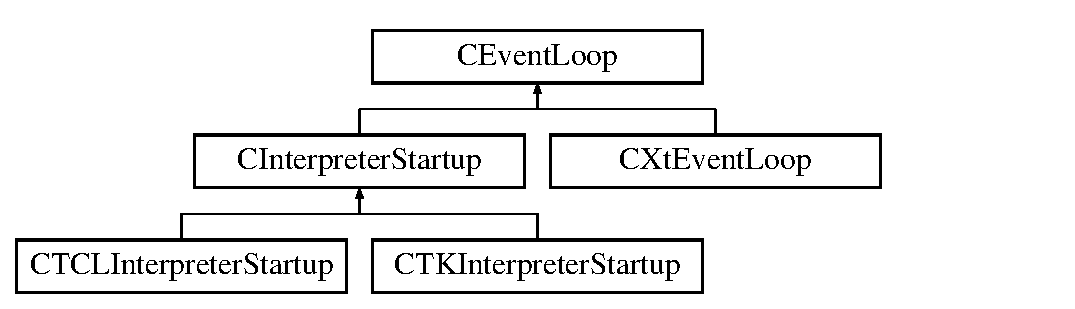
\includegraphics[height=3cm]{classCEventLoop}
\end{center}
\end{figure}
\subsection*{Public Methods}
\begin{CompactItemize}
\item 
{\bf CEvent\-Loop} ()
\item 
virtual {\bf $\sim$CEvent\-Loop} ()
\end{CompactItemize}
\subsection*{Static Public Methods}
\begin{CompactItemize}
\item 
CEvent\-Loop $\ast$ {\bf get\-Instance} ()
\end{CompactItemize}
\subsection*{Private Methods}
\begin{CompactItemize}
\item 
virtual int {\bf operator()} (int argc, char $\ast$$\ast$argv)=0
\begin{CompactList}\small\item\em Singleton instance.\item\end{CompactList}\item 
{\bf CEvent\-Loop} (const CEvent\-Loop \&a\-CEvent\-Loop)
\item 
CEvent\-Loop \& {\bf operator=} (const CEvent\-Loop \&a\-CEvent\-Loop)
\begin{CompactList}\small\item\em Not Implemented.\item\end{CompactList}\item 
int {\bf operator==} (const CEvent\-Loop \&a\-CEvent\-Loop) const
\begin{CompactList}\small\item\em Not Implemented.\item\end{CompactList}\end{CompactItemize}
\subsection*{Static Private Attributes}
\begin{CompactItemize}
\item 
CEvent\-Loop $\ast$ {\bf m\_\-p\-The\-Instance} = (CEvent\-Loop$\ast$)NULL
\end{CompactItemize}


\subsection{Detailed Description}
Encapsulates within a thread an application library which  runs it's own event loop. Examples are Xt and Tcl/Tk. These systems include their own mechanisms for detecting and dispatching events to application and framework specific code.

Attempting to instantiate more than one instance of an event  loop derived object results in a CDuplicate\-Singelton exception. Event loop derived processes implement operator() to  initiate an event loop how they are used depends on the iindividual framework. Each of these event loops is supposed to ensure that event dispatching to application level code is synchronized through the application's mutex. It is legal to synchronize all such events or an \char`\"{}appropriate subset\char`\"{}. 



Definition at line 315 of file CEvent\-Loop.h.

\subsection{Constructor \& Destructor Documentation}
\index{CEventLoop@{CEvent\-Loop}!CEventLoop@{CEventLoop}}
\index{CEventLoop@{CEventLoop}!CEventLoop@{CEvent\-Loop}}
\subsubsection{\setlength{\rightskip}{0pt plus 5cm}CEvent\-Loop::CEvent\-Loop ()}\label{classCEventLoop_a0}


The Constructs an event loop. Since event loops are singletons, this function throws a {\bf CDuplicate\-Singleton} {\rm (p.\,\pageref{classCDuplicateSingleton})} if the m\_\-p\-The\-Instance variable is not null. If the variable is null, it is filled in with this. 

Definition at line 323 of file CEvent\-Loop.cpp.

References m\_\-p\-The\-Instance.\index{CEventLoop@{CEvent\-Loop}!~CEventLoop@{$\sim$CEventLoop}}
\index{~CEventLoop@{$\sim$CEventLoop}!CEventLoop@{CEvent\-Loop}}
\subsubsection{\setlength{\rightskip}{0pt plus 5cm}CEvent\-Loop::$\sim$CEvent\-Loop ()\hspace{0.3cm}{\tt  [virtual]}}\label{classCEventLoop_a1}


The destructor sets the m\_\-p\-The\-Instance back to null. The assumption is that if derived classes catch the CDuplicate\-Singelton in their  constructors, they will re-throw it. Since such objects would be not fully constructed, they would not be destroyed and hence the instance pointer would not get spuriously deleted.



\begin{Desc}
\item[{\bf Bug: }]\par
There is no good way to enforce that {\bf CDuplicate\-Singleton} {\rm (p.\,\pageref{classCDuplicateSingleton})}'s don't result in spurious clears of the instance pointer.\end{Desc}
 

Definition at line 348 of file CEvent\-Loop.cpp.\index{CEventLoop@{CEvent\-Loop}!CEventLoop@{CEventLoop}}
\index{CEventLoop@{CEventLoop}!CEventLoop@{CEvent\-Loop}}
\subsubsection{\setlength{\rightskip}{0pt plus 5cm}CEvent\-Loop::CEvent\-Loop (const CEvent\-Loop \& {\em a\-CEvent\-Loop})\hspace{0.3cm}{\tt  [private]}}\label{classCEventLoop_c1}


Copy construction, assignment and comparison are not allowed. therefore they are declared as private and not implemented. 

\subsection{Member Function Documentation}
\index{CEventLoop@{CEvent\-Loop}!getInstance@{getInstance}}
\index{getInstance@{getInstance}!CEventLoop@{CEvent\-Loop}}
\subsubsection{\setlength{\rightskip}{0pt plus 5cm}CEvent\-Loop $\ast$ CEvent\-Loop::get\-Instance ()\hspace{0.3cm}{\tt  [static]}}\label{classCEventLoop_d0}


Retrieves the instance pointer. If the instance variable is null, throws CNo\-Such\-Object. 

Definition at line 365 of file CEvent\-Loop.cpp.

References m\_\-p\-The\-Instance.

Referenced by CTCLInterpreter\-Startup::Tcl\_\-Init(), and CTKInterpreter\-Startup::Tk\_\-Init().\index{CEventLoop@{CEvent\-Loop}!operator()@{operator()}}
\index{operator()@{operator()}!CEventLoop@{CEvent\-Loop}}
\subsubsection{\setlength{\rightskip}{0pt plus 5cm}virtual int CEvent\-Loop::operator() (int {\em argc}, char $\ast$$\ast$ {\em argv})\hspace{0.3cm}{\tt  [private, pure virtual]}}\label{classCEventLoop_c0}


Singleton instance.

Implemented by subclasses to provide the actual event loop functionality. int argc, char$\ast$$\ast$ argv provide a mechanism for passing parameters to the event loop thread as if it was run from a main program. 

Implemented in {\bf CInterpreter\-Startup} {\rm (p.\,\pageref{classCInterpreterStartup_c0})}, {\bf CTCLInterpreter\-Startup} {\rm (p.\,\pageref{classCTCLInterpreterStartup_c0})}, {\bf CTKInterpreter\-Startup} {\rm (p.\,\pageref{classCTKInterpreterStartup_c3})}, and {\bf CXt\-Event\-Loop} {\rm (p.\,\pageref{classCXtEventLoop_c0})}.\index{CEventLoop@{CEvent\-Loop}!operator=@{operator=}}
\index{operator=@{operator=}!CEventLoop@{CEvent\-Loop}}
\subsubsection{\setlength{\rightskip}{0pt plus 5cm}CEvent\-Loop\& CEvent\-Loop::operator= (const CEvent\-Loop \& {\em a\-CEvent\-Loop})\hspace{0.3cm}{\tt  [private]}}\label{classCEventLoop_c2}


Not Implemented.

\index{CEventLoop@{CEvent\-Loop}!operator==@{operator==}}
\index{operator==@{operator==}!CEventLoop@{CEvent\-Loop}}
\subsubsection{\setlength{\rightskip}{0pt plus 5cm}int CEvent\-Loop::operator== (const CEvent\-Loop \& {\em a\-CEvent\-Loop}) const\hspace{0.3cm}{\tt  [private]}}\label{classCEventLoop_c3}


Not Implemented.



\subsection{Member Data Documentation}
\index{CEventLoop@{CEvent\-Loop}!m_pTheInstance@{m\_\-pTheInstance}}
\index{m_pTheInstance@{m\_\-pTheInstance}!CEventLoop@{CEvent\-Loop}}
\subsubsection{\setlength{\rightskip}{0pt plus 5cm}CEvent\-Loop $\ast$ CEvent\-Loop::m\_\-p\-The\-Instance = (CEvent\-Loop$\ast$)NULL\hspace{0.3cm}{\tt  [static, private]}}\label{classCEventLoop_r0}


CEvent\-Loop$\ast$ m\_\-p\-The\-Instance Contains a pointer to the single event loop instance allowed. If there are no instances of the singleton, this pointer is null. Note that Get\-Instance will not attempt to create a new instance since it does not know which element of the class hierarchy to create. 

Definition at line 315 of file CEvent\-Loop.cpp.

Referenced by CEvent\-Loop(), and get\-Instance().

The documentation for this class was generated from the following files:\begin{CompactItemize}
\item 
{\bf CEvent\-Loop.h}\item 
{\bf CEvent\-Loop.cpp}\end{CompactItemize}

\section{CEvent\-Monitor  Class Reference}
\label{classCEventMonitor}\index{CEventMonitor@{CEvent\-Monitor}}
{\tt \#include $<$CEvent\-Monitor.h$>$}

Inheritance diagram for CEvent\-Monitor::\begin{figure}[H]
\begin{center}
\leavevmode
\includegraphics[height=4.63576cm]{classCEventMonitor}
\end{center}
\end{figure}
\subsection*{Public Types}
\begin{CompactItemize}
\item 
enum {\bf result} \{ {\bf Occurred} =  0, 
{\bf Timed\-Out} =  1, 
{\bf Error} =  2
 \}
\end{CompactItemize}
\subsection*{Public Methods}
\begin{CompactItemize}
\item 
{\bf CEvent\-Monitor} (bool am\_\-f\-Timed\-Wait=true)
\item 
{\bf CEvent\-Monitor} (const string \&r\-Name, bool am\_\-f\-Timed\-Wait=true)
\item 
{\bf CEvent\-Monitor} (const char $\ast$p\-Name, bool am\_\-f\-Timed\-Wait=true)
\item 
int {\bf operator==} (const CEvent\-Monitor \&a\-CEvent\-Monitor) const
\item 
virtual {\bf $\sim$CEvent\-Monitor} ()
\item 
timeval {\bf get\-Timeout} () const
\item 
bool {\bf get\-Timed\-Wait} () const
\item 
virtual {\bf CEvent\-Monitor::result} {\bf operator()} ()=0
\item 
virtual void {\bf set\-Timeout} (int n\-Timeout={\bf FOREVER})
\end{CompactItemize}
\subsection*{Protected Methods}
\begin{CompactItemize}
\item 
void {\bf set\-Timeout} (const timeval am\_\-tv\-Timeout)
\item 
void {\bf set\-Timed\-Wait} (const bool am\_\-f\-Timed\-Wait)
\end{CompactItemize}
\subsection*{Static Protected Methods}
\begin{CompactItemize}
\item 
string {\bf Get\-Auto\-Name} (const string \&r\-Base\-Name)
\begin{CompactList}\small\item\em Assign default name.\item\end{CompactList}\end{CompactItemize}
\subsection*{Private Methods}
\begin{CompactItemize}
\item 
{\bf CEvent\-Monitor} (const CEvent\-Monitor \&a\-CEvent\-Monitor)
\begin{CompactList}\small\item\em Copy construction is forbidden for now.\item\end{CompactList}\item 
CEvent\-Monitor {\bf operator=} (const {\bf CRegistered\-Object} \&a\-CEvent\-Monitor)
\begin{CompactList}\small\item\em Assignment is forbidden for now.\item\end{CompactList}\end{CompactItemize}
\subsection*{Private Attributes}
\begin{CompactItemize}
\item 
timeval {\bf m\_\-tv\-Timeout}
\item 
bool {\bf m\_\-f\-Timed\-Wait}
\end{CompactItemize}
\subsection*{Static Private Attributes}
\begin{CompactItemize}
\item 
unsigned int {\bf m\_\-n\-Auto\-Index}
\end{CompactItemize}


\subsection{Detailed Description}
$\backslash$class: CEvent\-Monitor

This file defines the CEvent\-Monitor class. CEvent\-Monitor is the ABC for all Event Monitors. An event monitor  provides event specific logic for waiting for external program events. operator() is expected to wait for an event to occur and return to  indicate if the event in fact did occur. 



Definition at line 326 of file CEvent\-Monitor.h.

\subsection{Member Enumeration Documentation}
\index{CEventMonitor@{CEvent\-Monitor}!result@{result}}
\index{result@{result}!CEventMonitor@{CEvent\-Monitor}}
\subsubsection{\setlength{\rightskip}{0pt plus 5cm}enum CEvent\-Monitor::result}\label{classCEventMonitor_s3}


Used to name autonamed objects \begin{Desc}
\item[Enumeration values:]\par
\begin{description}
\index{Occurred@{Occurred}!CEventMonitor@{CEvent\-Monitor}}\index{CEventMonitor@{CEventMonitor}!Occurred@{Occurred}}\item[{\em 
{\em Occurred}\label{classCEventMonitor_s3s0}
}]\index{TimedOut@{TimedOut}!CEventMonitor@{CEvent\-Monitor}}\index{CEventMonitor@{CEventMonitor}!TimedOut@{Timed\-Out}}\item[{\em 
{\em Timed\-Out}\label{classCEventMonitor_s3s1}
}]\index{Error@{Error}!CEventMonitor@{CEvent\-Monitor}}\index{CEventMonitor@{CEventMonitor}!Error@{Error}}\item[{\em 
{\em Error}\label{classCEventMonitor_s3s2}
}]\end{description}
\end{Desc}



Definition at line 335 of file CEvent\-Monitor.h.

Referenced by CEvent::On\-Event(), and CReactor::operator()().

\subsection{Constructor \& Destructor Documentation}
\index{CEventMonitor@{CEvent\-Monitor}!CEventMonitor@{CEventMonitor}}
\index{CEventMonitor@{CEventMonitor}!CEventMonitor@{CEvent\-Monitor}}
\subsubsection{\setlength{\rightskip}{0pt plus 5cm}CEvent\-Monitor::CEvent\-Monitor (bool {\em am\_\-f\-Timed\-Wait} = true)}\label{classCEventMonitor_a0}


Default constructor. An Event\-Monitor with name of the form Monitor\_\-nnn is created. The monitor is entered in to the \char`\"{}Monitors\char`\"{} registry of the  classified object registry returned from get\-CClassified\-Object\-Registry(). The name used is gaurenteed unique and can be queried via: {\bf get\-Name}() {\rm (p.\,\pageref{classCNamedObject_a6})}. 

Definition at line 312 of file CEvent\-Monitor.cpp.

References CNamed\-Object::Append\-Class\-Info(), m\_\-f\-Timed\-Wait, m\_\-tv\-Timeout, and Registry\-Name.\index{CEventMonitor@{CEvent\-Monitor}!CEventMonitor@{CEventMonitor}}
\index{CEventMonitor@{CEventMonitor}!CEventMonitor@{CEvent\-Monitor}}
\subsubsection{\setlength{\rightskip}{0pt plus 5cm}CEvent\-Monitor::CEvent\-Monitor (const string \& {\em r\-Name}, bool {\em am\_\-f\-Timed\-Wait} = true)}\label{classCEventMonitor_a1}


Constructs an Event\-Monitor given a name as an STL string, and a value of m\_\-f\-Timed\-Wait :\begin{Desc}
\item[Parameters: ]\par
\begin{description}
\item[{\em 
r\-Name}]- The desired name of the event monitor. \item[{\em 
am\_\-f\-Timed\-Wait}]- indicates whether or not the monitor is timed\end{description}
\end{Desc}
Throws:\begin{CompactItemize}
\item 
{\bf CDuplicate\-Name\-Exception} {\rm (p.\,\pageref{classCDuplicateNameException})} (indirectly) if a Reactor of this name already exists. \end{CompactItemize}


Definition at line 333 of file CEvent\-Monitor.cpp.

References CNamed\-Object::Append\-Class\-Info(), m\_\-f\-Timed\-Wait, m\_\-tv\-Timeout, and Registry\-Name.\index{CEventMonitor@{CEvent\-Monitor}!CEventMonitor@{CEventMonitor}}
\index{CEventMonitor@{CEventMonitor}!CEventMonitor@{CEvent\-Monitor}}
\subsubsection{\setlength{\rightskip}{0pt plus 5cm}CEvent\-Monitor::CEvent\-Monitor (const char $\ast$ {\em p\-Name}, bool {\em am\_\-f\-Timed\-Wait} = true)}\label{classCEventMonitor_a2}


Constructs an event monitor given its name as an ASCII string and an (optional) value for m\_\-f\-Timed\-Wait :\begin{Desc}
\item[Parameters: ]\par
\begin{description}
\item[{\em 
p\-Name}]- char$\ast$ pointer to the desired object name. \item[{\em 
am\_\-f\-Timed\-Wait}]- bool indicates whether the monitor is timed\end{description}
\end{Desc}
Throws: -{\bf CDuplicate\-Name\-Exception} {\rm (p.\,\pageref{classCDuplicateNameException})} (indirectly) if an event monitor of this name already exists. 

Definition at line 354 of file CEvent\-Monitor.cpp.

References CNamed\-Object::Append\-Class\-Info(), m\_\-f\-Timed\-Wait, m\_\-tv\-Timeout, and Registry\-Name.\index{CEventMonitor@{CEvent\-Monitor}!CEventMonitor@{CEventMonitor}}
\index{CEventMonitor@{CEventMonitor}!CEventMonitor@{CEvent\-Monitor}}
\subsubsection{\setlength{\rightskip}{0pt plus 5cm}CEvent\-Monitor::CEvent\-Monitor (const CEvent\-Monitor \& {\em a\-CEvent\-Monitor})\hspace{0.3cm}{\tt  [private]}}\label{classCEventMonitor_c0}


Copy construction is forbidden for now.

\index{CEventMonitor@{CEvent\-Monitor}!~CEventMonitor@{$\sim$CEventMonitor}}
\index{~CEventMonitor@{$\sim$CEventMonitor}!CEventMonitor@{CEvent\-Monitor}}
\subsubsection{\setlength{\rightskip}{0pt plus 5cm}CEvent\-Monitor::$\sim$CEvent\-Monitor ()\hspace{0.3cm}{\tt  [virtual]}}\label{classCEventMonitor_a4}


Destructor: Just ensure that we are removed from the Reactors registry before being destroyed. 

Definition at line 368 of file CEvent\-Monitor.cpp.

References CRegistered\-Object::get\-Registry(), Registry\-Name, and CClassified\-Object\-Registry::Remove().

\subsection{Member Function Documentation}
\index{CEventMonitor@{CEvent\-Monitor}!GetAutoName@{GetAutoName}}
\index{GetAutoName@{GetAutoName}!CEventMonitor@{CEvent\-Monitor}}
\subsubsection{\setlength{\rightskip}{0pt plus 5cm}string CEvent\-Monitor::Get\-Auto\-Name (const string \& {\em r\-Base\-Name})\hspace{0.3cm}{\tt  [static, protected]}}\label{classCEventMonitor_e0}


Assign default name.

Allocate a name for an object given some generic base name.  The final name is of the form: Base\-Name(m\_\-n\-Auto\-Index). 

Reimplemented from {\bf CNamed\-Object} {\rm (p.\,\pageref{classCNamedObject_e0})}.

Definition at line 397 of file CEvent\-Monitor.cpp.

References m\_\-n\-Auto\-Index.\index{CEventMonitor@{CEvent\-Monitor}!getTimedWait@{getTimedWait}}
\index{getTimedWait@{getTimedWait}!CEventMonitor@{CEvent\-Monitor}}
\subsubsection{\setlength{\rightskip}{0pt plus 5cm}bool CEvent\-Monitor::get\-Timed\-Wait () const\hspace{0.3cm}{\tt  [inline]}}\label{classCEventMonitor_a6}




Definition at line 375 of file CEvent\-Monitor.h.

References m\_\-f\-Timed\-Wait.

Referenced by CFd\-Monitor::Describe\-Self(), CFd\-Monitor::operator()(), and CBuffer\-Monitor$<$ T $>$::operator()().\index{CEventMonitor@{CEvent\-Monitor}!getTimeout@{getTimeout}}
\index{getTimeout@{getTimeout}!CEventMonitor@{CEvent\-Monitor}}
\subsubsection{\setlength{\rightskip}{0pt plus 5cm}timeval CEvent\-Monitor::get\-Timeout () const\hspace{0.3cm}{\tt  [inline]}}\label{classCEventMonitor_a5}




Definition at line 370 of file CEvent\-Monitor.h.

References m\_\-tv\-Timeout.

Referenced by CFd\-Monitor::Describe\-Self(), CTimer\-Monitor::operator()(), CLocation\-Monitor$<$ T $>$::operator()(), CFd\-Monitor::operator()(), and CBuffer\-Monitor$<$ T $>$::operator()().\index{CEventMonitor@{CEvent\-Monitor}!operator()@{operator()}}
\index{operator()@{operator()}!CEventMonitor@{CEvent\-Monitor}}
\subsubsection{\setlength{\rightskip}{0pt plus 5cm}virtual {\bf CEvent\-Monitor::result} CEvent\-Monitor::operator() ()\hspace{0.3cm}{\tt  [pure virtual]}}\label{classCEventMonitor_a7}




Implemented in {\bf CBuffer\-Monitor$<$ T $>$} {\rm (p.\,\pageref{classCBufferMonitor_a7})}, {\bf CFd\-Monitor} {\rm (p.\,\pageref{classCFdMonitor_a11})}, {\bf CLocation\-Monitor$<$ T $>$} {\rm (p.\,\pageref{classCLocationMonitor_a7})}, {\bf CServer\-Monitor} {\rm (p.\,\pageref{classCServerMonitor_a7})}, {\bf CTimer\-Monitor} {\rm (p.\,\pageref{classCTimerMonitor_a7})}, and {\bf CBuffer\-Monitor$<$ U $>$} {\rm (p.\,\pageref{classCBufferMonitor_a7})}.\index{CEventMonitor@{CEvent\-Monitor}!operator=@{operator=}}
\index{operator=@{operator=}!CEventMonitor@{CEvent\-Monitor}}
\subsubsection{\setlength{\rightskip}{0pt plus 5cm}CEvent\-Monitor CEvent\-Monitor::operator= (const {\bf CRegistered\-Object} \& {\em a\-CEvent\-Monitor})\hspace{0.3cm}{\tt  [private]}}\label{classCEventMonitor_c1}


Assignment is forbidden for now.



Reimplemented from {\bf CRegistered\-Object} {\rm (p.\,\pageref{classCRegisteredObject_c1})}.

Reimplemented in {\bf CFd\-Monitor} {\rm (p.\,\pageref{classCFdMonitor_c1})}.\index{CEventMonitor@{CEvent\-Monitor}!operator==@{operator==}}
\index{operator==@{operator==}!CEventMonitor@{CEvent\-Monitor}}
\subsubsection{\setlength{\rightskip}{0pt plus 5cm}int CEvent\-Monitor::operator== (const CEvent\-Monitor \& {\em a\-CEvent\-Monitor}) const\hspace{0.3cm}{\tt  [inline]}}\label{classCEventMonitor_a3}




Definition at line 348 of file CEvent\-Monitor.h.

References m\_\-f\-Timed\-Wait, m\_\-tv\-Timeout, and CRegistered\-Object::operator==().

Referenced by CTimer\-Monitor::operator==(), CLocation\-Monitor$<$ T $>$::operator==(), and CFd\-Monitor::operator==().\index{CEventMonitor@{CEvent\-Monitor}!setTimedWait@{setTimedWait}}
\index{setTimedWait@{setTimedWait}!CEventMonitor@{CEvent\-Monitor}}
\subsubsection{\setlength{\rightskip}{0pt plus 5cm}void CEvent\-Monitor::set\-Timed\-Wait (const bool {\em am\_\-f\-Timed\-Wait})\hspace{0.3cm}{\tt  [inline, protected]}}\label{classCEventMonitor_b1}




Definition at line 388 of file CEvent\-Monitor.h.

References m\_\-f\-Timed\-Wait.\index{CEventMonitor@{CEvent\-Monitor}!setTimeout@{setTimeout}}
\index{setTimeout@{setTimeout}!CEventMonitor@{CEvent\-Monitor}}
\subsubsection{\setlength{\rightskip}{0pt plus 5cm}void CEvent\-Monitor::set\-Timeout (int {\em n\-Timeout} = {\bf FOREVER})\hspace{0.3cm}{\tt  [virtual]}}\label{classCEventMonitor_a8}


void {\bf CEvent\-Monitor::set\-Timeout} {\rm (p.\,\pageref{classCEventMonitor_b0})}(int n\-Timeout=FOREVER)  Operation Type: mutator

Purpose: Sets the timeout. The length of the timeout is determined by the parameter in ms..  Special values: 0 - Poll (return instantly). FOREVER - Block until event. 

Reimplemented in {\bf CTimer\-Monitor} {\rm (p.\,\pageref{classCTimerMonitor_a9})}.

Definition at line 389 of file CEvent\-Monitor.cpp.

References m\_\-f\-Timed\-Wait, and m\_\-tv\-Timeout.\index{CEventMonitor@{CEvent\-Monitor}!setTimeout@{setTimeout}}
\index{setTimeout@{setTimeout}!CEventMonitor@{CEvent\-Monitor}}
\subsubsection{\setlength{\rightskip}{0pt plus 5cm}void CEvent\-Monitor::set\-Timeout (const timeval {\em am\_\-tv\-Timeout})\hspace{0.3cm}{\tt  [inline, protected]}}\label{classCEventMonitor_b0}




Definition at line 383 of file CEvent\-Monitor.h.

References m\_\-tv\-Timeout.

Referenced by main(), CEvent::operator()(), and CTimer\-Monitor::set\-Timeout().

\subsection{Member Data Documentation}
\index{CEventMonitor@{CEvent\-Monitor}!m_fTimedWait@{m\_\-fTimedWait}}
\index{m_fTimedWait@{m\_\-fTimedWait}!CEventMonitor@{CEvent\-Monitor}}
\subsubsection{\setlength{\rightskip}{0pt plus 5cm}bool CEvent\-Monitor::m\_\-f\-Timed\-Wait\hspace{0.3cm}{\tt  [private]}}\label{classCEventMonitor_o1}


Timeout length 

Definition at line 329 of file CEvent\-Monitor.h.

Referenced by CEvent\-Monitor(), get\-Timed\-Wait(), operator==(), set\-Timed\-Wait(), and set\-Timeout().\index{CEventMonitor@{CEvent\-Monitor}!m_nAutoIndex@{m\_\-nAutoIndex}}
\index{m_nAutoIndex@{m\_\-nAutoIndex}!CEventMonitor@{CEvent\-Monitor}}
\subsubsection{\setlength{\rightskip}{0pt plus 5cm}unsigned int CEvent\-Monitor::m\_\-n\-Auto\-Index\hspace{0.3cm}{\tt  [static, private]}}\label{classCEventMonitor_r0}


Timed wait? 

Reimplemented from {\bf CNamed\-Object} {\rm (p.\,\pageref{classCNamedObject_r0})}.

Referenced by Get\-Auto\-Name().\index{CEventMonitor@{CEvent\-Monitor}!m_tvTimeout@{m\_\-tvTimeout}}
\index{m_tvTimeout@{m\_\-tvTimeout}!CEventMonitor@{CEvent\-Monitor}}
\subsubsection{\setlength{\rightskip}{0pt plus 5cm}timeval CEvent\-Monitor::m\_\-tv\-Timeout\hspace{0.3cm}{\tt  [private]}}\label{classCEventMonitor_o0}




Definition at line 328 of file CEvent\-Monitor.h.

Referenced by CEvent\-Monitor(), get\-Timeout(), operator==(), and set\-Timeout().

The documentation for this class was generated from the following files:\begin{CompactItemize}
\item 
{\bf CEvent\-Monitor.h}\item 
{\bf CEvent\-Monitor.cpp}\end{CompactItemize}

\section{CException  Class Reference}
\label{classCException}\index{CException@{CException}}
{\tt \#include $<$CException.h$>$}

Inheritance diagram for CException::\begin{figure}[H]
\begin{center}
\leavevmode
\includegraphics[height=12cm]{classCException}
\end{center}
\end{figure}
\subsection*{Public Methods}
\begin{CompactItemize}
\item 
virtual {\bf $\sim$CException} ()
\item 
{\bf CException} (const char $\ast$psz\-Action)
\item 
{\bf CException} (const std::string \&rs\-Action)
\item 
{\bf CException} (const CException \&a\-CException)
\item 
CException \& {\bf operator=} (const CException \&a\-CException)
\item 
int {\bf operator==} (const CException \&a\-CException)
\item 
int {\bf operator!=} (const CException \&r\-Exception)
\item 
const char $\ast$ {\bf get\-Action} () const
\item 
virtual const char $\ast$ {\bf Reason\-Text} () const
\item 
virtual {\bf Int\_\-t} {\bf Reason\-Code} () const
\item 
const char $\ast$ {\bf Was\-Doing} () const
\end{CompactItemize}
\subsection*{Protected Methods}
\begin{CompactItemize}
\item 
void {\bf set\-Action} (const char $\ast$psz\-Action)
\item 
void {\bf set\-Action} (const std::string \&rs\-Action)
\item 
virtual void {\bf Do\-Assign} (const CException \&rhs)
\end{CompactItemize}
\subsection*{Private Attributes}
\begin{CompactItemize}
\item 
char {\bf m\_\-sz\-Action} [k\-ACTIONSIZE]
\end{CompactItemize}


\subsection{Detailed Description}
Base class for exceptions thrown  by the histogrammign subsystem. (could be used for any other subsystem for that matter). 



Definition at line 308 of file CException.h.

\subsection{Constructor \& Destructor Documentation}
\index{CException@{CException}!~CException@{$\sim$CException}}
\index{~CException@{$\sim$CException}!CException@{CException}}
\subsubsection{\setlength{\rightskip}{0pt plus 5cm}virtual CException::$\sim$CException ()\hspace{0.3cm}{\tt  [inline, virtual]}}\label{classCException_a0}




Definition at line 318 of file CException.h.\index{CException@{CException}!CException@{CException}}
\index{CException@{CException}!CException@{CException}}
\subsubsection{\setlength{\rightskip}{0pt plus 5cm}CException::CException (const char $\ast$ {\em psz\-Action})}\label{classCException_a1}




Definition at line 319 of file CException.cpp.

References set\-Action().\index{CException@{CException}!CException@{CException}}
\index{CException@{CException}!CException@{CException}}
\subsubsection{\setlength{\rightskip}{0pt plus 5cm}CException::CException (const std::string \& {\em rs\-Action})}\label{classCException_a2}




Definition at line 323 of file CException.cpp.

References set\-Action().\index{CException@{CException}!CException@{CException}}
\index{CException@{CException}!CException@{CException}}
\subsubsection{\setlength{\rightskip}{0pt plus 5cm}CException::CException (const CException \& {\em a\-CException})}\label{classCException_a3}




Definition at line 335 of file CException.cpp.

References Do\-Assign().

\subsection{Member Function Documentation}
\index{CException@{CException}!DoAssign@{DoAssign}}
\index{DoAssign@{DoAssign}!CException@{CException}}
\subsubsection{\setlength{\rightskip}{0pt plus 5cm}void CException::Do\-Assign (const CException \& {\em r\-Exception})\hspace{0.3cm}{\tt  [protected, virtual]}}\label{classCException_b2}


This is virtual to allow derived classes to override and chain calls to. 

Definition at line 465 of file CException.cpp.

References m\_\-sz\-Action, and set\-Action().

Referenced by CException(), and operator=().\index{CException@{CException}!getAction@{getAction}}
\index{getAction@{getAction}!CException@{CException}}
\subsubsection{\setlength{\rightskip}{0pt plus 5cm}const char$\ast$ CException::get\-Action () const\hspace{0.3cm}{\tt  [inline]}}\label{classCException_a7}




Definition at line 343 of file CException.h.

References m\_\-sz\-Action.

Referenced by Was\-Doing().\index{CException@{CException}!operator"!=@{operator"!=}}
\index{operator"!=@{operator"!=}!CException@{CException}}
\subsubsection{\setlength{\rightskip}{0pt plus 5cm}int CException::operator!= (const CException \& {\em r\-Exception})\hspace{0.3cm}{\tt  [inline]}}\label{classCException_a6}




Definition at line 335 of file CException.h.

References operator==().\index{CException@{CException}!operator=@{operator=}}
\index{operator=@{operator=}!CException@{CException}}
\subsubsection{\setlength{\rightskip}{0pt plus 5cm}CException \& CException::operator= (const CException \& {\em a\-CException})}\label{classCException_a4}




Definition at line 347 of file CException.cpp.

References Do\-Assign().

Referenced by CTCLException::operator=(), CTCPBad\-Socket\-State::operator=(), CRange\-Error::operator=(), CNo\-Such\-Object\-Exception::operator=(), CNo\-Such\-Link\-Exception::operator=(), CLink\-Failed\-Exception::operator=(), CIncompatible\-Monitor::operator=(), CErrno\-Exception::operator=(), CDuplicate\-Singleton::operator=(), and CDuplicate\-Name\-Exception::operator=().\index{CException@{CException}!operator==@{operator==}}
\index{operator==@{operator==}!CException@{CException}}
\subsubsection{\setlength{\rightskip}{0pt plus 5cm}int CException::operator== (const CException \& {\em a\-CException})}\label{classCException_a5}




Definition at line 363 of file CException.cpp.

References m\_\-sz\-Action.

Referenced by operator!=(), CTCLException::operator==(), CTCPNo\-Such\-Host::operator==(), CTCPBad\-Socket\-State::operator==(), CStream\-IOError::operator==(), CRange\-Error::operator==(), CNo\-Such\-Object\-Exception::operator==(), CNo\-Such\-Link\-Exception::operator==(), CLink\-Failed\-Exception::operator==(), CIncompatible\-Monitor::operator==(), CErrno\-Exception::operator==(), CDuplicate\-Singleton::operator==(), and CDuplicate\-Name\-Exception::operator==().\index{CException@{CException}!ReasonCode@{ReasonCode}}
\index{ReasonCode@{ReasonCode}!CException@{CException}}
\subsubsection{\setlength{\rightskip}{0pt plus 5cm}{\bf Int\_\-t} CException::Reason\-Code () const\hspace{0.3cm}{\tt  [virtual]}}\label{classCException_a9}


Returns a code which describes the reason for the exception . This is exception type specific and may be used to do detailed exception analysis and recovery. For example in the {\bf CErrno\-Exception} {\rm (p.\,\pageref{classCErrnoException})} class, the errno at the time of instantiation of the object is returned. The default returns -1 

Reimplemented in {\bf CTCPNo\-Such\-Host} {\rm (p.\,\pageref{classCTCPNoSuchHost_a8})}, {\bf CErrno\-Exception} {\rm (p.\,\pageref{classCErrnoException_a8})}, {\bf CRange\-Error} {\rm (p.\,\pageref{classCRangeError_a10})}, {\bf CStream\-IOError} {\rm (p.\,\pageref{classCStreamIOError_a9})}, and {\bf CTCLException} {\rm (p.\,\pageref{classCTCLException_a14})}.

Definition at line 407 of file CException.cpp.\index{CException@{CException}!ReasonText@{ReasonText}}
\index{ReasonText@{ReasonText}!CException@{CException}}
\subsubsection{\setlength{\rightskip}{0pt plus 5cm}const char $\ast$ CException::Reason\-Text () const\hspace{0.3cm}{\tt  [virtual]}}\label{classCException_a8}


Returns a const pointer to text which describes the reason the exception was thrown. This is exception type specific. The default action returns a pointer to the constant string: \char`\"{}Unspecified Exception\char`\"{} 

Reimplemented in {\bf CDuplicate\-Name\-Exception} {\rm (p.\,\pageref{classCDuplicateNameException_a10})}, {\bf CDuplicate\-Singleton} {\rm (p.\,\pageref{classCDuplicateSingleton_a10})}, {\bf CIncompatible\-Monitor} {\rm (p.\,\pageref{classCIncompatibleMonitor_a7})}, {\bf CLink\-Failed\-Exception} {\rm (p.\,\pageref{classCLinkFailedException_a12})}, {\bf CNo\-Such\-Link\-Exception} {\rm (p.\,\pageref{classCNoSuchLinkException_a12})}, {\bf CNo\-Such\-Object\-Exception} {\rm (p.\,\pageref{classCNoSuchObjectException_a10})}, {\bf CTCPBad\-Socket\-State} {\rm (p.\,\pageref{classCTCPBadSocketState_a7})}, {\bf CTCPConnection\-Failed} {\rm (p.\,\pageref{classCTCPConnectionFailed_a7})}, {\bf CTCPConnection\-Lost} {\rm (p.\,\pageref{classCTCPConnectionLost_a7})}, {\bf CTCPNo\-Such\-Host} {\rm (p.\,\pageref{classCTCPNoSuchHost_a7})}, {\bf CTCPNo\-Such\-Service} {\rm (p.\,\pageref{classCTCPNoSuchService_a6})}, {\bf CErrno\-Exception} {\rm (p.\,\pageref{classCErrnoException_a7})}, {\bf CRange\-Error} {\rm (p.\,\pageref{classCRangeError_a9})}, {\bf CStream\-IOError} {\rm (p.\,\pageref{classCStreamIOError_a8})}, and {\bf CTCLException} {\rm (p.\,\pageref{classCTCLException_a13})}.

Definition at line 385 of file CException.cpp.\index{CException@{CException}!setAction@{setAction}}
\index{setAction@{setAction}!CException@{CException}}
\subsubsection{\setlength{\rightskip}{0pt plus 5cm}void CException::set\-Action (const std::string \& {\em rs\-Action})\hspace{0.3cm}{\tt  [protected]}}\label{classCException_b1}




Definition at line 448 of file CException.cpp.

References set\-Action().\index{CException@{CException}!setAction@{setAction}}
\index{setAction@{setAction}!CException@{CException}}
\subsubsection{\setlength{\rightskip}{0pt plus 5cm}void CException::set\-Action (const char $\ast$ {\em psz\-Action})\hspace{0.3cm}{\tt  [protected]}}\label{classCException_b0}




Definition at line 443 of file CException.cpp.

References m\_\-sz\-Action.

Referenced by CException(), Do\-Assign(), and set\-Action().\index{CException@{CException}!WasDoing@{WasDoing}}
\index{WasDoing@{WasDoing}!CException@{CException}}
\subsubsection{\setlength{\rightskip}{0pt plus 5cm}const char $\ast$ CException::Was\-Doing () const}\label{classCException_a10}


Returns a const pointer to m\_\-sz\-Action. This is intended to describe the action  which was occuring when the exception was thrown. 

Definition at line 427 of file CException.cpp.

References get\-Action().

Referenced by CTCPNo\-Such\-Host::Reason\-Text(), CTCPBad\-Socket\-State::Reason\-Text(), and CIncompatible\-Monitor::Reason\-Text().

\subsection{Member Data Documentation}
\index{CException@{CException}!m_szAction@{m\_\-szAction}}
\index{m_szAction@{m\_\-szAction}!CException@{CException}}
\subsubsection{\setlength{\rightskip}{0pt plus 5cm}char CException::m\_\-sz\-Action[k\-ACTIONSIZE]\hspace{0.3cm}{\tt  [private]}}\label{classCException_o0}




Definition at line 312 of file CException.h.

Referenced by Do\-Assign(), get\-Action(), operator==(), and set\-Action().

The documentation for this class was generated from the following files:\begin{CompactItemize}
\item 
{\bf CException.cpp}\item 
{\bf CException.h}\end{CompactItemize}

\section{CFd\-Monitor  Class Reference}
\label{classCFdMonitor}\index{CFdMonitor@{CFd\-Monitor}}
{\tt \#include $<$CFd\-Monitor.h$>$}

Inheritance diagram for CFd\-Monitor::\begin{figure}[H]
\begin{center}
\leavevmode
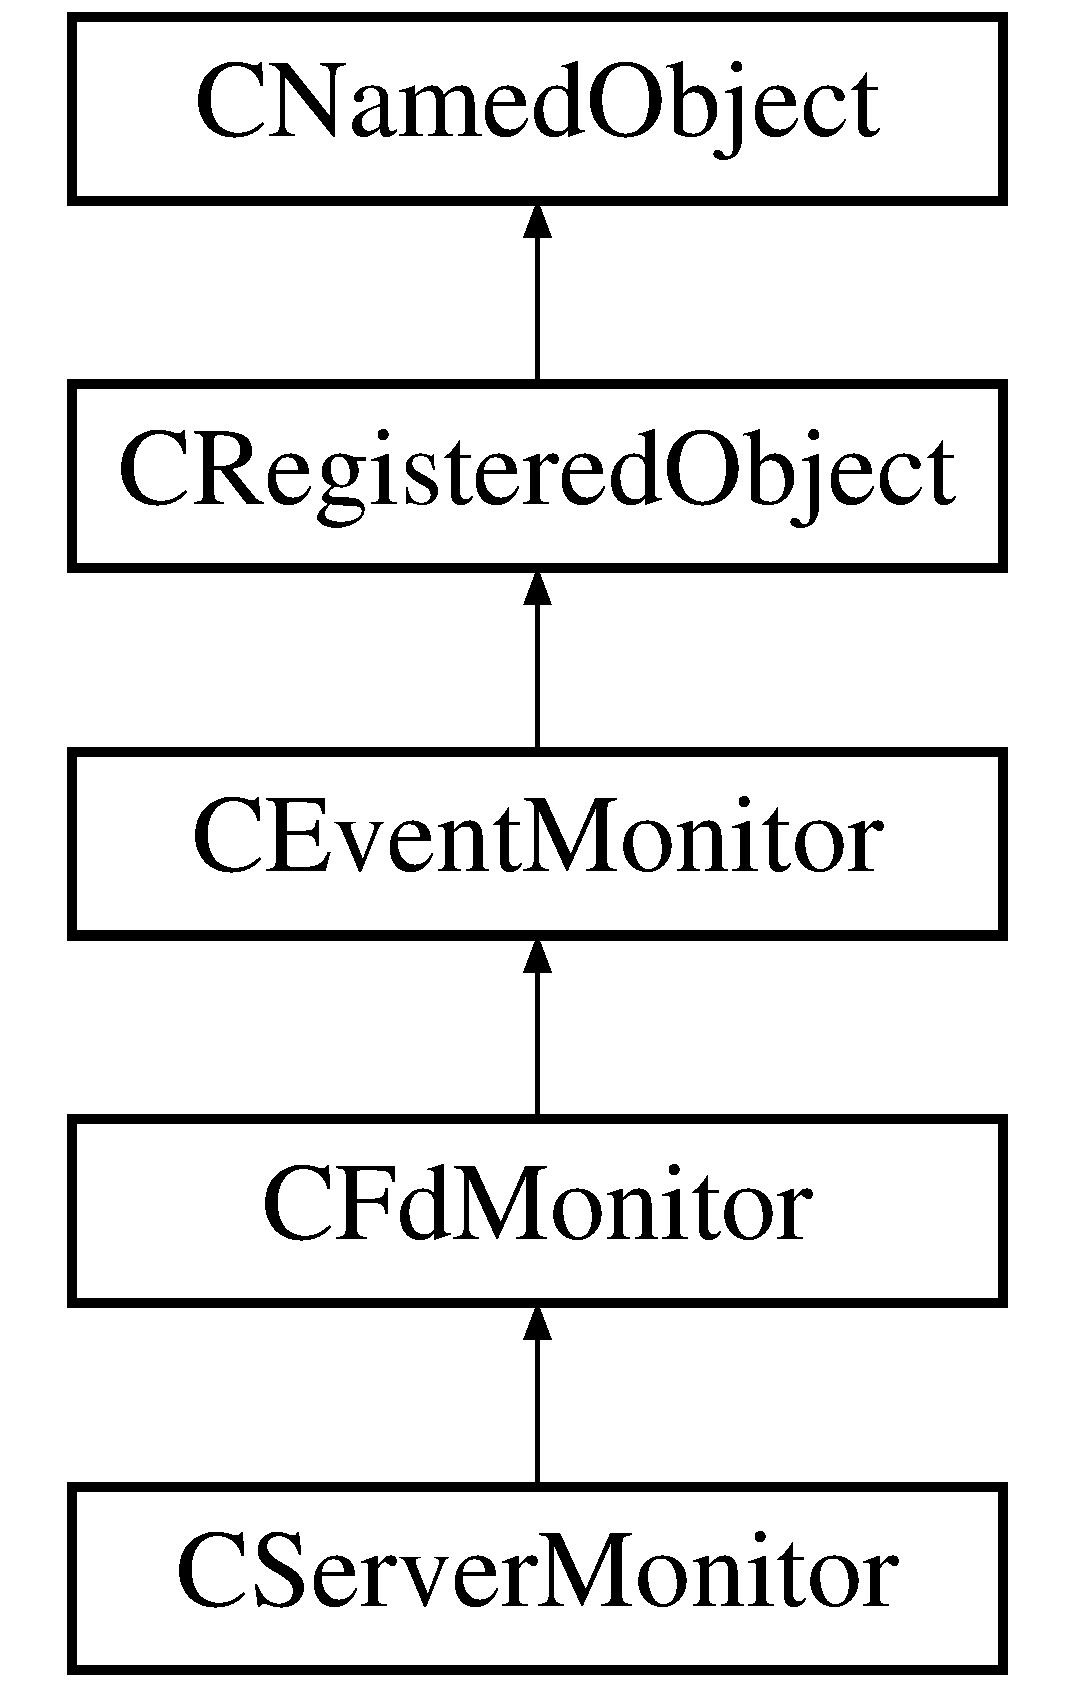
\includegraphics[height=5cm]{classCFdMonitor}
\end{center}
\end{figure}
\subsection*{Public Types}
\begin{CompactItemize}
\item 
enum {\bf Fd\-Conditions} \{ {\bf FD\_\-READABLE} = 0, 
{\bf FD\_\-WRITABLE} = 1, 
{\bf FD\_\-EXCEPTION} = 2
 \}
\end{CompactItemize}
\subsection*{Public Methods}
\begin{CompactItemize}
\item 
{\bf CFd\-Monitor} (int am\_\-n\-Fd, bool am\_\-f\-Timed\-Wait=true)
\item 
{\bf CFd\-Monitor} (const string \&r\-Name, int am\_\-n\-Fd, bool am\_\-f\-Timed\-Wait=true)
\item 
{\bf CFd\-Monitor} (const char $\ast$p\-Name, int am\_\-n\-Fd, bool am\_\-f\-Timed\-Wait=true)
\item 
int {\bf operator==} (const CFd\-Monitor \&a\-CFd\-Monitor) const
\item 
virtual {\bf $\sim$CFd\-Monitor} ()
\item 
int {\bf get\-Fd} () const
\item 
unsigned int {\bf get\-Condition\-Mask} () const
\item 
int {\bf get\-Last\-Event\-Mask} () const
\item 
void {\bf Monitor\-Readable} (bool f\-Readable=true)
\item 
void {\bf Monitor\-Writable} (bool f\-Writable=true)
\item 
void {\bf Monitor\-Exceptions} (bool f\-Exception=true)
\item 
virtual {\bf CEvent\-Monitor::result} {\bf operator()} ()
\item 
virtual string {\bf Describe\-Self} ()
\end{CompactItemize}
\subsection*{Protected Methods}
\begin{CompactItemize}
\item 
void {\bf set\-Fd} (const int am\_\-n\-Fd)
\item 
void {\bf set\-Condition\-Mask} (const unsigned int am\_\-n\-Condition\-Mask)
\item 
void {\bf set\-Last\-Event\-Mask} (const int am\_\-f\-Last\-Event\-Mask)
\end{CompactItemize}
\subsection*{Private Methods}
\begin{CompactItemize}
\item 
{\bf CFd\-Monitor} (const {\bf CRegistered\-Object} \&a\-CRegistered\-Object)
\item 
CFd\-Monitor {\bf operator=} (const {\bf CRegistered\-Object} \&a\-CRegistered\-Object)
\begin{CompactList}\small\item\em Assignment is forbidden for now.\item\end{CompactList}\end{CompactItemize}
\subsection*{Private Attributes}
\begin{CompactItemize}
\item 
int {\bf m\_\-n\-Fd}
\item 
unsigned int {\bf m\_\-n\-Condition\-Mask}
\item 
int {\bf m\_\-f\-Last\-Event\-Mask}
\end{CompactItemize}


\subsection{Detailed Description}
$\backslash$class: {\bf CFd\-Monitor.h}

This file defines the CFd\-Monitor class. Monitors activity on a file descriptor. A file descriptior can be  monitored for the logical or of any of the following conditions: Readable Writable Exception

Monitoring is done via the select(2) system service. Note that this can yield some unexpected results. For example, in some operating systems, tape drives are never considered readable without blocking.

Author: Jason Venema NSCL Michigan State University East Lansing, MI 48824-1321 mailto:{\tt venemaja@msu.edu} 



Definition at line 319 of file CFd\-Monitor.h.

\subsection{Member Enumeration Documentation}
\index{CFdMonitor@{CFd\-Monitor}!FdConditions@{FdConditions}}
\index{FdConditions@{FdConditions}!CFdMonitor@{CFd\-Monitor}}
\subsubsection{\setlength{\rightskip}{0pt plus 5cm}enum CFd\-Monitor::Fd\-Conditions}\label{classCFdMonitor_s3}


Mask of the last set of bits to be detected \begin{Desc}
\item[Enumeration values:]\par
\begin{description}
\index{FD_READABLE@{FD\_\-READABLE}!CFdMonitor@{CFd\-Monitor}}\index{CFdMonitor@{CFdMonitor}!FD_READABLE@{FD\_\-READABLE}}\item[{\em 
{\em FD\_\-READABLE}\label{classCFdMonitor_s3s0}
}]\index{FD_WRITABLE@{FD\_\-WRITABLE}!CFdMonitor@{CFd\-Monitor}}\index{CFdMonitor@{CFdMonitor}!FD_WRITABLE@{FD\_\-WRITABLE}}\item[{\em 
{\em FD\_\-WRITABLE}\label{classCFdMonitor_s3s1}
}]\index{FD_EXCEPTION@{FD\_\-EXCEPTION}!CFdMonitor@{CFd\-Monitor}}\index{CFdMonitor@{CFdMonitor}!FD_EXCEPTION@{FD\_\-EXCEPTION}}\item[{\em 
{\em FD\_\-EXCEPTION}\label{classCFdMonitor_s3s2}
}]\end{description}
\end{Desc}



Definition at line 329 of file CFd\-Monitor.h.

Referenced by CFd\-Reactor::On\-Event().

\subsection{Constructor \& Destructor Documentation}
\index{CFdMonitor@{CFd\-Monitor}!CFdMonitor@{CFdMonitor}}
\index{CFdMonitor@{CFdMonitor}!CFdMonitor@{CFd\-Monitor}}
\subsubsection{\setlength{\rightskip}{0pt plus 5cm}CFd\-Monitor::CFd\-Monitor (int {\em am\_\-n\-Fd}, bool {\em am\_\-f\-Timed\-Wait} = true)\hspace{0.3cm}{\tt  [inline]}}\label{classCFdMonitor_a0}




Definition at line 338 of file CFd\-Monitor.h.

References CNamed\-Object::Append\-Class\-Info(), m\_\-f\-Last\-Event\-Mask, m\_\-n\-Condition\-Mask, and m\_\-n\-Fd.\index{CFdMonitor@{CFd\-Monitor}!CFdMonitor@{CFdMonitor}}
\index{CFdMonitor@{CFdMonitor}!CFdMonitor@{CFd\-Monitor}}
\subsubsection{\setlength{\rightskip}{0pt plus 5cm}CFd\-Monitor::CFd\-Monitor (const string \& {\em r\-Name}, int {\em am\_\-n\-Fd}, bool {\em am\_\-f\-Timed\-Wait} = true)\hspace{0.3cm}{\tt  [inline]}}\label{classCFdMonitor_a1}




Definition at line 345 of file CFd\-Monitor.h.

References CNamed\-Object::Append\-Class\-Info(), m\_\-f\-Last\-Event\-Mask, m\_\-n\-Condition\-Mask, and m\_\-n\-Fd.\index{CFdMonitor@{CFd\-Monitor}!CFdMonitor@{CFdMonitor}}
\index{CFdMonitor@{CFdMonitor}!CFdMonitor@{CFd\-Monitor}}
\subsubsection{\setlength{\rightskip}{0pt plus 5cm}CFd\-Monitor::CFd\-Monitor (const char $\ast$ {\em p\-Name}, int {\em am\_\-n\-Fd}, bool {\em am\_\-f\-Timed\-Wait} = true)\hspace{0.3cm}{\tt  [inline]}}\label{classCFdMonitor_a2}




Definition at line 352 of file CFd\-Monitor.h.

References CNamed\-Object::Append\-Class\-Info(), m\_\-f\-Last\-Event\-Mask, m\_\-n\-Condition\-Mask, and m\_\-n\-Fd.\index{CFdMonitor@{CFd\-Monitor}!~CFdMonitor@{$\sim$CFdMonitor}}
\index{~CFdMonitor@{$\sim$CFdMonitor}!CFdMonitor@{CFd\-Monitor}}
\subsubsection{\setlength{\rightskip}{0pt plus 5cm}virtual CFd\-Monitor::$\sim$CFd\-Monitor ()\hspace{0.3cm}{\tt  [inline, virtual]}}\label{classCFdMonitor_a4}




Definition at line 369 of file CFd\-Monitor.h.\index{CFdMonitor@{CFd\-Monitor}!CFdMonitor@{CFdMonitor}}
\index{CFdMonitor@{CFdMonitor}!CFdMonitor@{CFd\-Monitor}}
\subsubsection{\setlength{\rightskip}{0pt plus 5cm}CFd\-Monitor::CFd\-Monitor (const {\bf CRegistered\-Object} \& {\em a\-CRegistered\-Object})\hspace{0.3cm}{\tt  [private]}}\label{classCFdMonitor_c0}




\subsection{Member Function Documentation}
\index{CFdMonitor@{CFd\-Monitor}!DescribeSelf@{DescribeSelf}}
\index{DescribeSelf@{DescribeSelf}!CFdMonitor@{CFd\-Monitor}}
\subsubsection{\setlength{\rightskip}{0pt plus 5cm}string CFd\-Monitor::Describe\-Self ()\hspace{0.3cm}{\tt  [virtual]}}\label{classCFdMonitor_a12}


Operation Type: Interface Implementation

Purpose: Uses the m\_\-s\-Class\-Path member to describe its class path, and returns a string containing this and its data member values. 

Reimplemented from {\bf CNamed\-Object} {\rm (p.\,\pageref{classCNamedObject_a8})}.

Reimplemented in {\bf CServer\-Monitor} {\rm (p.\,\pageref{classCServerMonitor_a8})}.

Definition at line 420 of file CFd\-Monitor.cpp.

References CNamed\-Object::Describe\-Self(), CEvent\-Monitor::get\-Timed\-Wait(), CEvent\-Monitor::get\-Timeout(), and m\_\-n\-Fd.

Referenced by main().\index{CFdMonitor@{CFd\-Monitor}!getConditionMask@{getConditionMask}}
\index{getConditionMask@{getConditionMask}!CFdMonitor@{CFd\-Monitor}}
\subsubsection{\setlength{\rightskip}{0pt plus 5cm}unsigned int CFd\-Monitor::get\-Condition\-Mask () const\hspace{0.3cm}{\tt  [inline]}}\label{classCFdMonitor_a6}




Definition at line 386 of file CFd\-Monitor.h.

References m\_\-n\-Condition\-Mask.

Referenced by main().\index{CFdMonitor@{CFd\-Monitor}!getFd@{getFd}}
\index{getFd@{getFd}!CFdMonitor@{CFd\-Monitor}}
\subsubsection{\setlength{\rightskip}{0pt plus 5cm}int CFd\-Monitor::get\-Fd () const\hspace{0.3cm}{\tt  [inline]}}\label{classCFdMonitor_a5}




Definition at line 381 of file CFd\-Monitor.h.

References m\_\-n\-Fd.

Referenced by CFd\-Reactor::On\-Event().\index{CFdMonitor@{CFd\-Monitor}!getLastEventMask@{getLastEventMask}}
\index{getLastEventMask@{getLastEventMask}!CFdMonitor@{CFd\-Monitor}}
\subsubsection{\setlength{\rightskip}{0pt plus 5cm}int CFd\-Monitor::get\-Last\-Event\-Mask () const\hspace{0.3cm}{\tt  [inline]}}\label{classCFdMonitor_a7}




Definition at line 391 of file CFd\-Monitor.h.

References m\_\-f\-Last\-Event\-Mask.

Referenced by CFd\-Reactor::On\-Event().\index{CFdMonitor@{CFd\-Monitor}!MonitorExceptions@{MonitorExceptions}}
\index{MonitorExceptions@{MonitorExceptions}!CFdMonitor@{CFd\-Monitor}}
\subsubsection{\setlength{\rightskip}{0pt plus 5cm}void CFd\-Monitor::Monitor\-Exceptions (bool {\em f\-Exception} = true)}\label{classCFdMonitor_a10}


Operation Type: Mutator

Purpose: Sets or clears the FD\_\-EXCEPTION bit in m\_\-n\-Condition\-Mask. 

Definition at line 344 of file CFd\-Monitor.cpp.

References FD\_\-EXCEPTION, and m\_\-n\-Condition\-Mask.

Referenced by main().\index{CFdMonitor@{CFd\-Monitor}!MonitorReadable@{MonitorReadable}}
\index{MonitorReadable@{MonitorReadable}!CFdMonitor@{CFd\-Monitor}}
\subsubsection{\setlength{\rightskip}{0pt plus 5cm}void CFd\-Monitor::Monitor\-Readable (bool {\em f\-Readable} = true)}\label{classCFdMonitor_a8}


Operation Type: Mutator

Purpose: Sets or clears the FD\_\-READABLE bit in m\_\-n\-Condition\-Mask. 

Definition at line 314 of file CFd\-Monitor.cpp.

References FD\_\-READABLE, and m\_\-n\-Condition\-Mask.

Referenced by main().\index{CFdMonitor@{CFd\-Monitor}!MonitorWritable@{MonitorWritable}}
\index{MonitorWritable@{MonitorWritable}!CFdMonitor@{CFd\-Monitor}}
\subsubsection{\setlength{\rightskip}{0pt plus 5cm}void CFd\-Monitor::Monitor\-Writable (bool {\em f\-Writable} = true)}\label{classCFdMonitor_a9}


Operation Type: Mutator

Purpose:  Sets or clears the FD\_\-WRITABLE bit in the m\_\-n\-Condition\-Mask attribute. 

Definition at line 329 of file CFd\-Monitor.cpp.

References FD\_\-WRITABLE, and m\_\-n\-Condition\-Mask.

Referenced by main().\index{CFdMonitor@{CFd\-Monitor}!operator()@{operator()}}
\index{operator()@{operator()}!CFdMonitor@{CFd\-Monitor}}
\subsubsection{\setlength{\rightskip}{0pt plus 5cm}{\bf CEvent\-Monitor::result} CFd\-Monitor::operator() ()\hspace{0.3cm}{\tt  [virtual]}}\label{classCFdMonitor_a11}


Operation Type: Interface Implementation

Purpose:

Implements a wait for a single file descriptor event as described in the mask. Returns one of: Occured - one of the masked conditions occured. Timed\-Out - Timeout was enabled and none of the conditions occured within the timeout. Error - An error condition ocurred. 

Implements {\bf CEvent\-Monitor} {\rm (p.\,\pageref{classCEventMonitor_a7})}.

Reimplemented in {\bf CServer\-Monitor} {\rm (p.\,\pageref{classCServerMonitor_a7})}.

Definition at line 367 of file CFd\-Monitor.cpp.

References CEvent\-Monitor::Error, FD\_\-EXCEPTION, FD\_\-READABLE, FD\_\-WRITABLE, CEvent\-Monitor::get\-Timed\-Wait(), CEvent\-Monitor::get\-Timeout(), m\_\-f\-Last\-Event\-Mask, m\_\-n\-Condition\-Mask, m\_\-n\-Fd, CEvent\-Monitor::Occurred, and CEvent\-Monitor::Timed\-Out.\index{CFdMonitor@{CFd\-Monitor}!operator=@{operator=}}
\index{operator=@{operator=}!CFdMonitor@{CFd\-Monitor}}
\subsubsection{\setlength{\rightskip}{0pt plus 5cm}CFd\-Monitor CFd\-Monitor::operator= (const {\bf CRegistered\-Object} \& {\em a\-CRegistered\-Object})\hspace{0.3cm}{\tt  [private]}}\label{classCFdMonitor_c1}


Assignment is forbidden for now.



Reimplemented from {\bf CEvent\-Monitor} {\rm (p.\,\pageref{classCEventMonitor_c1})}.

Referenced by CServer\-Monitor::operator=().\index{CFdMonitor@{CFd\-Monitor}!operator==@{operator==}}
\index{operator==@{operator==}!CFdMonitor@{CFd\-Monitor}}
\subsubsection{\setlength{\rightskip}{0pt plus 5cm}int CFd\-Monitor::operator== (const CFd\-Monitor \& {\em a\-CFd\-Monitor}) const\hspace{0.3cm}{\tt  [inline]}}\label{classCFdMonitor_a3}




Definition at line 360 of file CFd\-Monitor.h.

References m\_\-f\-Last\-Event\-Mask, m\_\-n\-Condition\-Mask, m\_\-n\-Fd, and CEvent\-Monitor::operator==().

Referenced by CServer\-Monitor::operator==().\index{CFdMonitor@{CFd\-Monitor}!setConditionMask@{setConditionMask}}
\index{setConditionMask@{setConditionMask}!CFdMonitor@{CFd\-Monitor}}
\subsubsection{\setlength{\rightskip}{0pt plus 5cm}void CFd\-Monitor::set\-Condition\-Mask (const unsigned int {\em am\_\-n\-Condition\-Mask})\hspace{0.3cm}{\tt  [inline, protected]}}\label{classCFdMonitor_b1}




Definition at line 404 of file CFd\-Monitor.h.

References m\_\-n\-Condition\-Mask.\index{CFdMonitor@{CFd\-Monitor}!setFd@{setFd}}
\index{setFd@{setFd}!CFdMonitor@{CFd\-Monitor}}
\subsubsection{\setlength{\rightskip}{0pt plus 5cm}void CFd\-Monitor::set\-Fd (const int {\em am\_\-n\-Fd})\hspace{0.3cm}{\tt  [inline, protected]}}\label{classCFdMonitor_b0}




Definition at line 399 of file CFd\-Monitor.h.

References m\_\-n\-Fd.\index{CFdMonitor@{CFd\-Monitor}!setLastEventMask@{setLastEventMask}}
\index{setLastEventMask@{setLastEventMask}!CFdMonitor@{CFd\-Monitor}}
\subsubsection{\setlength{\rightskip}{0pt plus 5cm}void CFd\-Monitor::set\-Last\-Event\-Mask (const int {\em am\_\-f\-Last\-Event\-Mask})\hspace{0.3cm}{\tt  [inline, protected]}}\label{classCFdMonitor_b2}




Definition at line 409 of file CFd\-Monitor.h.

References m\_\-f\-Last\-Event\-Mask.

\subsection{Member Data Documentation}
\index{CFdMonitor@{CFd\-Monitor}!m_fLastEventMask@{m\_\-fLastEventMask}}
\index{m_fLastEventMask@{m\_\-fLastEventMask}!CFdMonitor@{CFd\-Monitor}}
\subsubsection{\setlength{\rightskip}{0pt plus 5cm}int CFd\-Monitor::m\_\-f\-Last\-Event\-Mask\hspace{0.3cm}{\tt  [private]}}\label{classCFdMonitor_o2}


Conditions which will be monitored by  the monitor for the file descriptor. 

Definition at line 324 of file CFd\-Monitor.h.

Referenced by CFd\-Monitor(), get\-Last\-Event\-Mask(), operator()(), operator==(), and set\-Last\-Event\-Mask().\index{CFdMonitor@{CFd\-Monitor}!m_nConditionMask@{m\_\-nConditionMask}}
\index{m_nConditionMask@{m\_\-nConditionMask}!CFdMonitor@{CFd\-Monitor}}
\subsubsection{\setlength{\rightskip}{0pt plus 5cm}unsigned int CFd\-Monitor::m\_\-n\-Condition\-Mask\hspace{0.3cm}{\tt  [private]}}\label{classCFdMonitor_o1}


File descriptor which will be monitored by the monitor 

Definition at line 322 of file CFd\-Monitor.h.

Referenced by CFd\-Monitor(), get\-Condition\-Mask(), Monitor\-Exceptions(), Monitor\-Readable(), Monitor\-Writable(), operator()(), operator==(), and set\-Condition\-Mask().\index{CFdMonitor@{CFd\-Monitor}!m_nFd@{m\_\-nFd}}
\index{m_nFd@{m\_\-nFd}!CFdMonitor@{CFd\-Monitor}}
\subsubsection{\setlength{\rightskip}{0pt plus 5cm}int CFd\-Monitor::m\_\-n\-Fd\hspace{0.3cm}{\tt  [private]}}\label{classCFdMonitor_o0}




Definition at line 321 of file CFd\-Monitor.h.

Referenced by CFd\-Monitor(), Describe\-Self(), get\-Fd(), operator()(), operator==(), and set\-Fd().

The documentation for this class was generated from the following files:\begin{CompactItemize}
\item 
{\bf CFd\-Monitor.h}\item 
{\bf CFd\-Monitor.cpp}\end{CompactItemize}

\section{CFd\-Reactor  Class Reference}
\label{classCFdReactor}\index{CFdReactor@{CFd\-Reactor}}
{\tt \#include $<$CFd\-Reactor.h$>$}

Inheritance diagram for CFd\-Reactor::\begin{figure}[H]
\begin{center}
\leavevmode
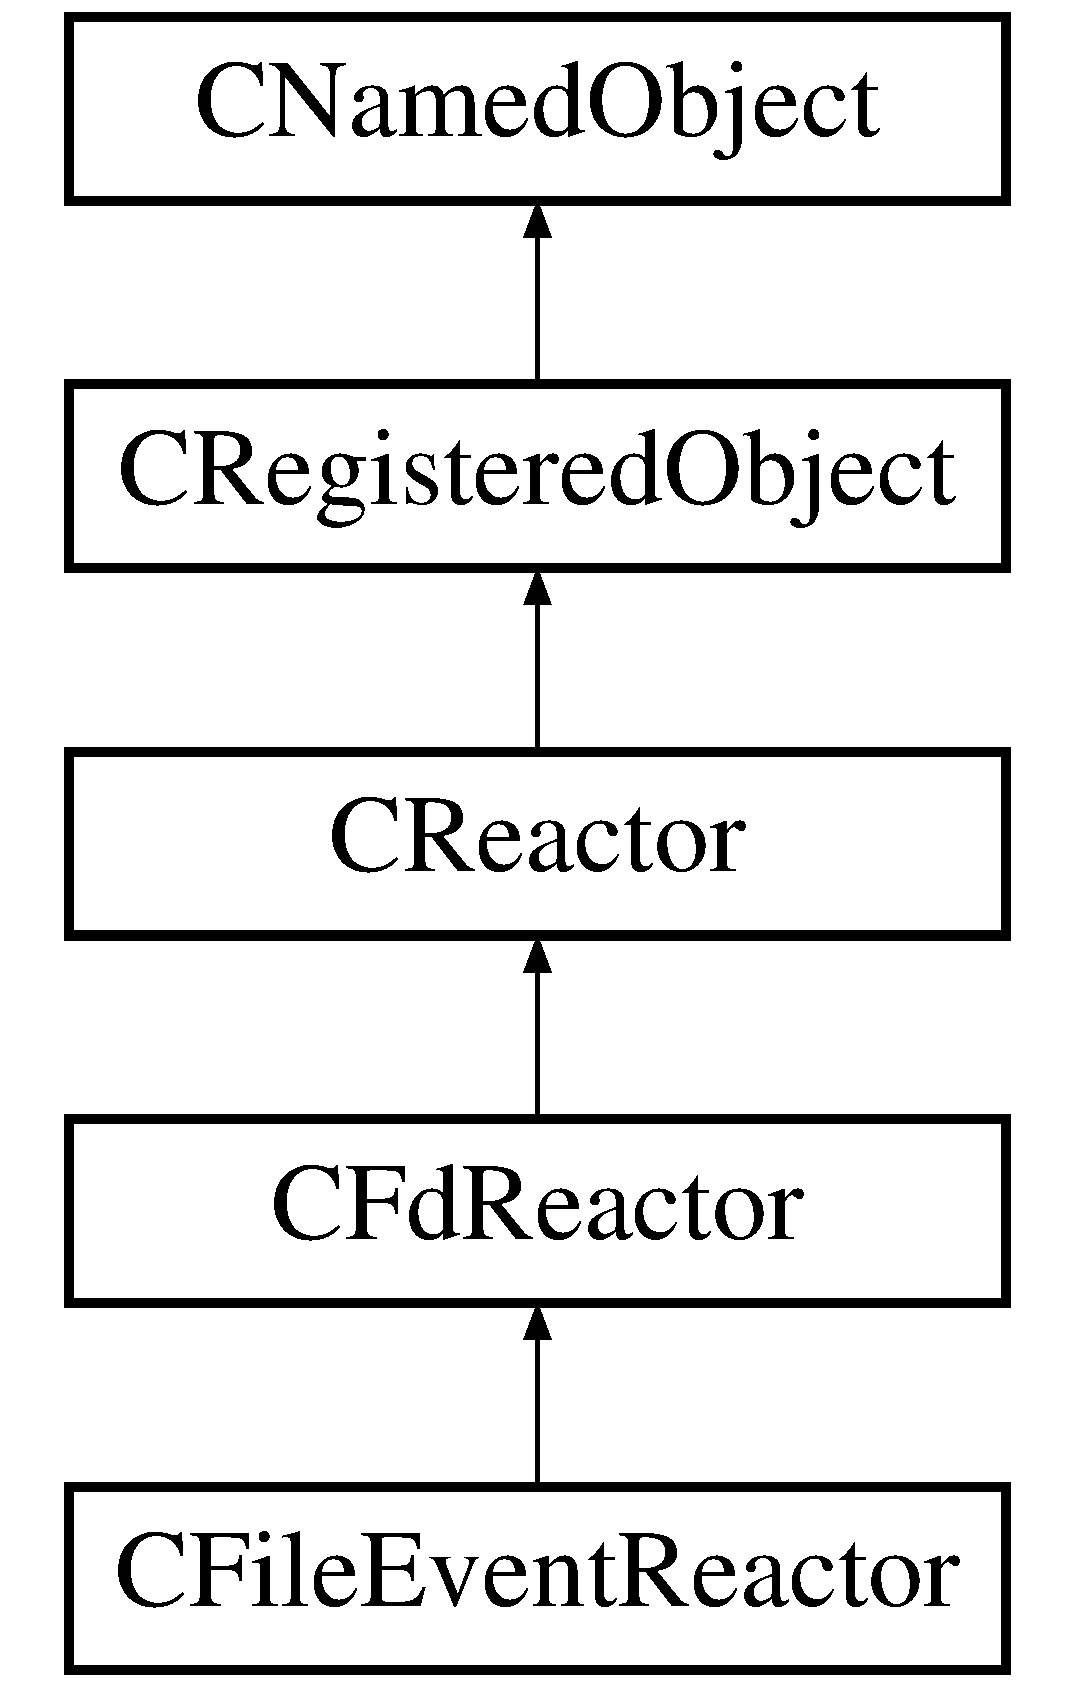
\includegraphics[height=5cm]{classCFdReactor}
\end{center}
\end{figure}
\subsection*{Public Methods}
\begin{CompactItemize}
\item 
{\bf CFd\-Reactor} ()
\item 
{\bf CFd\-Reactor} (const char $\ast$p\-Name)
\item 
{\bf CFd\-Reactor} (const string \&r\-Name)
\item 
virtual {\bf $\sim$CFd\-Reactor} ()
\item 
int {\bf operator==} (const CFd\-Reactor \&a\-CFd\-Reactor) const
\begin{CompactList}\small\item\em Operator== Equality Operator.\item\end{CompactList}\item 
virtual void {\bf On\-Event} ({\bf CEvent\-Monitor} \&r\-Monitor)
\item 
virtual void {\bf On\-Readable} ({\bf CFd\-Monitor} \&r\-Monitor, int fd)
\item 
virtual void {\bf On\-Writable} ({\bf CFd\-Monitor} \&r\-Monitor, int fd)
\item 
virtual void {\bf On\-Exception} ({\bf CFd\-Monitor} \&r\-Monitor, int fd)
\end{CompactItemize}
\subsection*{Private Methods}
\begin{CompactItemize}
\item 
{\bf CFd\-Reactor} (const CFd\-Reactor \&a\-CFd\-Reactor)
\begin{CompactList}\small\item\em Copy construction is prohibited.\item\end{CompactList}\item 
CFd\-Reactor \& {\bf operator=} (const CFd\-Reactor \&a\-CFd\-Reactor)
\begin{CompactList}\small\item\em Operator= Assignment Operator - Prohibited.\item\end{CompactList}\end{CompactItemize}


\subsection{Detailed Description}
Base class for file descriptor reactors: Fd reactors react to events on a file descriptor. This abstract base class must be subclassed by the programmer to provide application specific behavior. 



Definition at line 317 of file CFd\-Reactor.h.

\subsection{Constructor \& Destructor Documentation}
\index{CFdReactor@{CFd\-Reactor}!CFdReactor@{CFdReactor}}
\index{CFdReactor@{CFdReactor}!CFdReactor@{CFd\-Reactor}}
\subsubsection{\setlength{\rightskip}{0pt plus 5cm}CFd\-Reactor::CFd\-Reactor ()}\label{classCFdReactor_a0}


Default constructor: Creates a file descriptor reactor which autonamed. Such fd reactors in general are not named in a memorable way. 

Definition at line 300 of file CFd\-Reactor.cpp.

References CNamed\-Object::Append\-Class\-Info().\index{CFdReactor@{CFd\-Reactor}!CFdReactor@{CFdReactor}}
\index{CFdReactor@{CFdReactor}!CFdReactor@{CFd\-Reactor}}
\subsubsection{\setlength{\rightskip}{0pt plus 5cm}CFd\-Reactor::CFd\-Reactor (const char $\ast$ {\em p\-Name})}\label{classCFdReactor_a1}


Constructor for a named reactor. Creates a file descriptor reactor which is given a memorable name by the object's client. \begin{Desc}
\item[Parameters: ]\par
\begin{description}
\item[{\em 
p\-Name}]-Pointer to object name in ASCIZ form. \end{description}
\end{Desc}


Definition at line 310 of file CFd\-Reactor.cpp.

References CNamed\-Object::Append\-Class\-Info().\index{CFdReactor@{CFd\-Reactor}!CFdReactor@{CFdReactor}}
\index{CFdReactor@{CFdReactor}!CFdReactor@{CFd\-Reactor}}
\subsubsection{\setlength{\rightskip}{0pt plus 5cm}CFd\-Reactor::CFd\-Reactor (const string \& {\em r\-Name})}\label{classCFdReactor_a2}


Constructor for a named reactor. Creates a file descriptor reactor which is given a memorable name by the object's client. \begin{Desc}
\item[Parameters: ]\par
\begin{description}
\item[{\em 
r\-Name}]- reference to an STL String which has the object's name. \end{description}
\end{Desc}


Definition at line 321 of file CFd\-Reactor.cpp.

References CNamed\-Object::Append\-Class\-Info().\index{CFdReactor@{CFd\-Reactor}!CFdReactor@{CFdReactor}}
\index{CFdReactor@{CFdReactor}!CFdReactor@{CFd\-Reactor}}
\subsubsection{\setlength{\rightskip}{0pt plus 5cm}CFd\-Reactor::CFd\-Reactor (const CFd\-Reactor \& {\em a\-CFd\-Reactor})\hspace{0.3cm}{\tt  [private]}}\label{classCFdReactor_c0}


Copy construction is prohibited.

\index{CFdReactor@{CFd\-Reactor}!~CFdReactor@{$\sim$CFdReactor}}
\index{~CFdReactor@{$\sim$CFdReactor}!CFdReactor@{CFd\-Reactor}}
\subsubsection{\setlength{\rightskip}{0pt plus 5cm}CFd\-Reactor::$\sim$CFd\-Reactor ()\hspace{0.3cm}{\tt  [virtual]}}\label{classCFdReactor_a3}




Definition at line 327 of file CFd\-Reactor.cpp.

\subsection{Member Function Documentation}
\index{CFdReactor@{CFd\-Reactor}!OnEvent@{OnEvent}}
\index{OnEvent@{OnEvent}!CFdReactor@{CFd\-Reactor}}
\subsubsection{\setlength{\rightskip}{0pt plus 5cm}void CFd\-Reactor::On\-Event ({\bf CEvent\-Monitor} \& {\em r\-Monitor})\hspace{0.3cm}{\tt  [virtual]}}\label{classCFdReactor_a5}


EDispatches an incomming event from an Fd\-Monitor to one or more of the following member functions:\begin{CompactItemize}
\item 
On\-Readble - The file is readable.\item 
On\-Writable - The file is writable.\item 
On\-Exception - The file has an exceptional condition.\end{CompactItemize}
NOTE: We can only dispatch to conditions the monitor is looking for.

Throws:\begin{CompactItemize}
\item 
CIncompatible\-Monitor\-Exception - If the monitor cannot be cast to a {\bf CFd\-Monitor} {\rm (p.\,\pageref{classCFdMonitor})} object.\end{CompactItemize}
\begin{Desc}
\item[Parameters: ]\par
\begin{description}
\item[{\em 
r\-Monitor}]- Reference to the monitor which caused us to be invoked. This should be an object which lives in the {\bf CFd\-Monitor} {\rm (p.\,\pageref{classCFdMonitor})} branch of the CMonitor class hierarchy. \end{description}
\end{Desc}


Reimplemented from {\bf CReactor} {\rm (p.\,\pageref{classCReactor_a6})}.

Definition at line 357 of file CFd\-Reactor.cpp.

References CFd\-Monitor::FD\_\-EXCEPTION, CFd\-Monitor::FD\_\-READABLE, CFd\-Monitor::FD\_\-WRITABLE, CFd\-Monitor::Fd\-Conditions, CFd\-Monitor::get\-Fd(), CFd\-Monitor::get\-Last\-Event\-Mask(), On\-Exception(), On\-Readable(), and On\-Writable().\index{CFdReactor@{CFd\-Reactor}!OnException@{OnException}}
\index{OnException@{OnException}!CFdReactor@{CFd\-Reactor}}
\subsubsection{\setlength{\rightskip}{0pt plus 5cm}void CFd\-Reactor::On\-Exception ({\bf CFd\-Monitor} \& {\em r\-Monitor}, int {\em fd})\hspace{0.3cm}{\tt  [virtual]}}\label{classCFdReactor_a8}


Called when the file associated with the event monitor has an \char`\"{}exceptional condition\char`\"{}.. Actual use of this Reactor involves subclassing the monitor and overriding On\-Exception if you care about processing exceptional conditions. 

Reimplemented in {\bf CFile\-Event\-Reactor} {\rm (p.\,\pageref{classCFileEvent_1_1CFileEventReactor_a4})}.

Definition at line 409 of file CFd\-Reactor.cpp.

Referenced by On\-Event().\index{CFdReactor@{CFd\-Reactor}!OnReadable@{OnReadable}}
\index{OnReadable@{OnReadable}!CFdReactor@{CFd\-Reactor}}
\subsubsection{\setlength{\rightskip}{0pt plus 5cm}void CFd\-Reactor::On\-Readable ({\bf CFd\-Monitor} \& {\em r\-Monitor}, int {\em fd})\hspace{0.3cm}{\tt  [virtual]}}\label{classCFdReactor_a6}


Called when the file associated with the event monitor becomes readable. Actual use of this Reactor involves subclassing the monitor and overriding On\-Readable if you care about reading the file. 

Reimplemented in {\bf CFile\-Event\-Reactor} {\rm (p.\,\pageref{classCFileEvent_1_1CFileEventReactor_a2})}.

Definition at line 389 of file CFd\-Reactor.cpp.

Referenced by On\-Event().\index{CFdReactor@{CFd\-Reactor}!OnWritable@{OnWritable}}
\index{OnWritable@{OnWritable}!CFdReactor@{CFd\-Reactor}}
\subsubsection{\setlength{\rightskip}{0pt plus 5cm}void CFd\-Reactor::On\-Writable ({\bf CFd\-Monitor} \& {\em r\-Monitor}, int {\em fd})\hspace{0.3cm}{\tt  [virtual]}}\label{classCFdReactor_a7}


Called when the file associated with the event monitor becomes writable. Actual use of this Reactor involves subclassing the monitor and overriding On\-Writable if you care about writing the file. 

Reimplemented in {\bf CFile\-Event\-Reactor} {\rm (p.\,\pageref{classCFileEvent_1_1CFileEventReactor_a3})}.

Definition at line 399 of file CFd\-Reactor.cpp.

Referenced by On\-Event().\index{CFdReactor@{CFd\-Reactor}!operator=@{operator=}}
\index{operator=@{operator=}!CFdReactor@{CFd\-Reactor}}
\subsubsection{\setlength{\rightskip}{0pt plus 5cm}CFd\-Reactor\& CFd\-Reactor::operator= (const CFd\-Reactor \& {\em a\-CFd\-Reactor})\hspace{0.3cm}{\tt  [private]}}\label{classCFdReactor_c1}


Operator= Assignment Operator - Prohibited.

\index{CFdReactor@{CFd\-Reactor}!operator==@{operator==}}
\index{operator==@{operator==}!CFdReactor@{CFd\-Reactor}}
\subsubsection{\setlength{\rightskip}{0pt plus 5cm}int CFd\-Reactor::operator== (const CFd\-Reactor \& {\em a\-CFd\-Reactor}) const}\label{classCFdReactor_a4}


Operator== Equality Operator.



Definition at line 332 of file CFd\-Reactor.cpp.

References CReactor::operator==().

The documentation for this class was generated from the following files:\begin{CompactItemize}
\item 
{\bf CFd\-Reactor.h}\item 
{\bf CFd\-Reactor.cpp}\end{CompactItemize}

\section{CFile\-Event  Class Reference}
\label{classCFileEvent}\index{CFileEvent@{CFile\-Event}}
{\tt \#include $<$CFile\-Event.h$>$}

Inheritance diagram for CFile\-Event::\begin{figure}[H]
\begin{center}
\leavevmode
\includegraphics[height=5cm]{classCFileEvent}
\end{center}
\end{figure}
\subsection*{Public Methods}
\begin{CompactItemize}
\item 
{\bf CFile\-Event} (int fd, int access={\bf readable})
\item 
{\bf CFile\-Event} (const char $\ast$p\-Name, int flags=O\_\-RDONLY, int access={\bf readable})
\item 
{\bf CFile\-Event} (const string \&r\-Name, int flags=O\_\-RDONLY, int access={\bf readable})
\item 
{\bf CFile\-Event} (int fd, const char $\ast$p\-Obj\-Name, int access={\bf readable})
\item 
{\bf CFile\-Event} (const char $\ast$p\-Obj\-Name, const char $\ast$p\-Name, int flags=O\_\-RDONLY, int access={\bf readable})
\item 
{\bf CFile\-Event} (const char $\ast$p\-Obj\-Name, const string \&r\-Name, int flags=O\_\-RDONLY, int access={\bf readable})
\item 
{\bf CFile\-Event} (int fd, const string \&r\-Obj\-Name, int access={\bf readable})
\item 
{\bf CFile\-Event} (const string \&r\-Obj\-Name, const char $\ast$pname, int flags=O\_\-RDONLY, int access={\bf readable})
\item 
{\bf CFile\-Event} (const string \&r\-Obj\-Name, const string \&r\-Name, int flags=O\_\-RDONLY, int access={\bf readable})
\item 
{\bf $\sim$CFile\-Event} ()
\item 
int {\bf get\-Fd} () const
\item 
int {\bf get\-Close\-On\-Destory} () const
\item 
void {\bf Monitor\-Readable} (bool f\-Readable=true)
\item 
void {\bf Monitor\-Writable} (bool f\-Writable=true)
\item 
void {\bf Monitor\-Exceptions} (bool f\-Except=true)
\item 
virtual void {\bf On\-Readable} (istream \&r\-Stream)
\item 
virtual void {\bf On\-Writable} (ostream \&r\-Stream)
\item 
virtual void {\bf On\-Exception} (iostream \&fd)
\item 
virtual void {\bf On\-Timeout} (iostream \&str)
\item 
virtual string {\bf Describe\-Self} ()
\end{CompactItemize}
\subsection*{Static Public Attributes}
\begin{CompactItemize}
\item 
int {\bf readable} = 1
\begin{CompactList}\small\item\em Bitmask for readable monitoring.\item\end{CompactList}\item 
int {\bf writeable} = 2
\begin{CompactList}\small\item\em Bitmask for writable monitoring.\item\end{CompactList}\item 
int {\bf exceptions} = 4
\begin{CompactList}\small\item\em Bitmask for exception monitoring.\item\end{CompactList}\end{CompactItemize}
\subsection*{Protected Methods}
\begin{CompactItemize}
\item 
void {\bf Exit} (int status)
\item 
void {\bf Setup\-Monitor} (int Access\-Mask)
\item 
{\bf CFd\-Monitor} $\ast$ {\bf Create\-Monitor} (const char $\ast$p\-Filename, const char $\ast$p\-Monitor, int flags)
\end{CompactItemize}
\subsection*{Private Methods}
\begin{CompactItemize}
\item 
{\bf CFile\-Event} (const CFile\-Event \&r\-Event)
\item 
CFile\-Event \& {\bf operator=} (const CFile\-Event \&rhs)
\item 
int {\bf operator==} (const CFile\-Event \&r\-Event)
\end{CompactItemize}
\subsection*{Private Attributes}
\begin{CompactItemize}
\item 
int {\bf m\_\-n\-Fd}
\begin{CompactList}\small\item\em File descriptor.\item\end{CompactList}\item 
bool {\bf m\_\-f\-Close\-On\-Destroy}
\begin{CompactList}\small\item\em true if we opened the file.\item\end{CompactList}\end{CompactItemize}


\subsection{Detailed Description}
C lass providing functionality for  file descriptor events. Must be derived and  operator() implemented to provide application functionality. 



Definition at line 333 of file CFile\-Event.h.

\subsection{Constructor \& Destructor Documentation}
\index{CFileEvent@{CFile\-Event}!CFileEvent@{CFileEvent}}
\index{CFileEvent@{CFileEvent}!CFileEvent@{CFile\-Event}}
\subsubsection{\setlength{\rightskip}{0pt plus 5cm}CFile\-Event::CFile\-Event (int {\em fd}, int {\em access} = {\bf readable})}\label{classCFileEvent_a0}


Construct an anonymous file event from a file descriptor,  The file monitor is a {\bf CFd\-Monitor} {\rm (p.\,\pageref{classCFdMonitor})} directly constructed from the fd via new. \begin{Desc}
\item[Parameters: ]\par
\begin{description}
\item[{\em 
fd}]- File descriptor to open on the file. \item[{\em 
access}]- Bitwise or of access required to file. \end{description}
\end{Desc}


Definition at line 404 of file CFile\-Event.cpp.

References CNamed\-Object::Append\-Class\-Info(), CNamed\-Object::Get\-Auto\-Name(), m\_\-f\-Close\-On\-Destroy, m\_\-n\-Fd, and Setup\-Monitor().\index{CFileEvent@{CFile\-Event}!CFileEvent@{CFileEvent}}
\index{CFileEvent@{CFileEvent}!CFileEvent@{CFile\-Event}}
\subsubsection{\setlength{\rightskip}{0pt plus 5cm}CFile\-Event::CFile\-Event (const char $\ast$ {\em p\-Name}, int {\em flags} = O\_\-RDONLY, int {\em access} = {\bf readable})}\label{classCFileEvent_a1}


Construct an anonymous file event from a filename as a const char$\ast$ A file is opened and created with Create\-Monitor. \begin{Desc}
\item[Parameters: ]\par
\begin{description}
\item[{\em 
p\-Name}]- Name of file to open/create. \item[{\em 
flags}]- open(2) flags. \item[{\em 
access}]- Bitwise access requirements for the file. \end{description}
\end{Desc}


Definition at line 421 of file CFile\-Event.cpp.

References CNamed\-Object::Append\-Class\-Info(), and Setup\-Monitor().\index{CFileEvent@{CFile\-Event}!CFileEvent@{CFileEvent}}
\index{CFileEvent@{CFileEvent}!CFileEvent@{CFile\-Event}}
\subsubsection{\setlength{\rightskip}{0pt plus 5cm}CFile\-Event::CFile\-Event (const string \& {\em r\-Name}, int {\em flags} = O\_\-RDONLY, int {\em access} = {\bf readable})}\label{classCFileEvent_a2}


Construct an anonymous file event from a filename as a const string\& A file is opened and created with {\bf Create\-Monitor}() {\rm (p.\,\pageref{classCFileEvent_b2})} \begin{Desc}
\item[Parameters: ]\par
\begin{description}
\item[{\em 
r\-Name}]- Nameof the file to open/create \item[{\em 
flags}]- open(2) flags.. \item[{\em 
access}]- Bitwise access requirements for the file. \end{description}
\end{Desc}


Definition at line 436 of file CFile\-Event.cpp.

References CNamed\-Object::Append\-Class\-Info(), and Setup\-Monitor().\index{CFileEvent@{CFile\-Event}!CFileEvent@{CFileEvent}}
\index{CFileEvent@{CFileEvent}!CFileEvent@{CFile\-Event}}
\subsubsection{\setlength{\rightskip}{0pt plus 5cm}CFile\-Event::CFile\-Event (int {\em fd}, const char $\ast$ {\em p\-Obj\-Name}, int {\em access} = {\bf readable})}\label{classCFileEvent_a3}


Construct a named file event from a char$\ast$ object name, and a file descriptor. The {\bf CFd\-Monitor} {\rm (p.\,\pageref{classCFdMonitor})} is directly new'd into existence in the operation. \begin{Desc}
\item[Parameters: ]\par
\begin{description}
\item[{\em 
p\-Obj\-Name}]- Pointer to object name. \item[{\em 
fd}]- File descriptor on already open file to monitor. \item[{\em 
access}]- Bitwise or of the desired access to the file.\end{description}
\end{Desc}
Throws:\begin{CompactItemize}
\item 
{\bf CDuplicate\-Name\-Exception} {\rm (p.\,\pageref{classCDuplicateNameException})} - if this object or any subobject already have this name. \end{CompactItemize}


Definition at line 463 of file CFile\-Event.cpp.

References CNamed\-Object::Append\-Class\-Info(), and Setup\-Monitor().\index{CFileEvent@{CFile\-Event}!CFileEvent@{CFileEvent}}
\index{CFileEvent@{CFileEvent}!CFileEvent@{CFile\-Event}}
\subsubsection{\setlength{\rightskip}{0pt plus 5cm}CFile\-Event::CFile\-Event (const char $\ast$ {\em p\-Obj\-Name}, const char $\ast$ {\em p\-Filename}, int {\em flags} = O\_\-RDONLY, int {\em access} = {\bf readable})}\label{classCFileEvent_a4}


Construct a named file event from a char$\ast$ object name and a char$\ast$ filename. The {\bf CFd\-Monitor} {\rm (p.\,\pageref{classCFdMonitor})} is created by Create\-Monitor. \begin{Desc}
\item[Parameters: ]\par
\begin{description}
\item[{\em 
p\-Obj\-Name}]- Name to give to all the objects. \item[{\em 
p\-Filename}]- Name of the file to access. \item[{\em 
flags}]- open(2) flags. \item[{\em 
access}]- Bitwise or of the access rights desired to the file.\end{description}
\end{Desc}
Throws:\begin{CompactItemize}
\item 
{\bf CDuplicate\-Name\-Exception} {\rm (p.\,\pageref{classCDuplicateNameException})} - if this object or any subobject already have this name. \end{CompactItemize}


Definition at line 489 of file CFile\-Event.cpp.

References CNamed\-Object::Append\-Class\-Info(), and Setup\-Monitor().\index{CFileEvent@{CFile\-Event}!CFileEvent@{CFileEvent}}
\index{CFileEvent@{CFileEvent}!CFileEvent@{CFile\-Event}}
\subsubsection{\setlength{\rightskip}{0pt plus 5cm}CFile\-Event::CFile\-Event (const char $\ast$ {\em p\-Obj\-Name}, const string \& {\em r\-Filename}, int {\em flags} = O\_\-RDONLY, int {\em access} = {\bf readable})}\label{classCFileEvent_a5}


Constructs a named file event given a char$\ast$ object name and a string\& filename. The monitor is created via Create\-Monitor. \begin{Desc}
\item[Parameters: ]\par
\begin{description}
\item[{\em 
p\-Obj\-Name}]- Pointer to the name of the object  \item[{\em 
r\-Filename}]- Reference to the name of the file \item[{\em 
flags}]- open(2) flags.. \item[{\em 
access}]- Bitmask specifying access desired.\end{description}
\end{Desc}
Throws:\begin{CompactItemize}
\item 
{\bf CDuplicate\-Name\-Exception} {\rm (p.\,\pageref{classCDuplicateNameException})} - if this object or any subobject already have this name. \end{CompactItemize}


Definition at line 513 of file CFile\-Event.cpp.

References CNamed\-Object::Append\-Class\-Info(), and Setup\-Monitor().\index{CFileEvent@{CFile\-Event}!CFileEvent@{CFileEvent}}
\index{CFileEvent@{CFileEvent}!CFileEvent@{CFile\-Event}}
\subsubsection{\setlength{\rightskip}{0pt plus 5cm}CFile\-Event::CFile\-Event (int {\em fd}, const string \& {\em r\-Obj\-Name}, int {\em access} = {\bf readable})}\label{classCFileEvent_a6}


Construct a file event from a string\& object name and an fd. The Monitor can be created directly via new \begin{Desc}
\item[Parameters: ]\par
\begin{description}
\item[{\em 
r\-Obj\-Name}]- Reference to the name of the object. \item[{\em 
fd}]- File descriptor to monitor. \item[{\em 
access}]- Desired access to the file.\end{description}
\end{Desc}
Throws:\begin{CompactItemize}
\item 
{\bf CDuplicate\-Name\-Exception} {\rm (p.\,\pageref{classCDuplicateNameException})} - if this object or any subobject already have this name. \end{CompactItemize}


Definition at line 539 of file CFile\-Event.cpp.

References CNamed\-Object::Append\-Class\-Info(), and Setup\-Monitor().\index{CFileEvent@{CFile\-Event}!CFileEvent@{CFileEvent}}
\index{CFileEvent@{CFileEvent}!CFileEvent@{CFile\-Event}}
\subsubsection{\setlength{\rightskip}{0pt plus 5cm}CFile\-Event::CFile\-Event (const string \& {\em r\-Obj\-Name}, const char $\ast$ {\em p\-Filename}, int {\em flags} = O\_\-RDONLY, int {\em access} = {\bf readable})}\label{classCFileEvent_a7}


Construct a file event from a string\& object name and a char$\ast$ filename. The monitor is created via Create\-Monitor. \begin{Desc}
\item[Parameters: ]\par
\begin{description}
\item[{\em 
r\-Obj\-Name}]- Reference to the name of the object. \item[{\em 
p\-Filename}]- Pointer to the filename. \item[{\em 
flags}]- open(2) flags. \item[{\em 
access}]- Bitmask specifying the desired file access.\end{description}
\end{Desc}
Throws:\begin{CompactItemize}
\item 
{\bf CDuplicate\-Name\-Exception} {\rm (p.\,\pageref{classCDuplicateNameException})} - if this object or any subobject already have this name. \end{CompactItemize}


Definition at line 562 of file CFile\-Event.cpp.

References CNamed\-Object::Append\-Class\-Info(), and Setup\-Monitor().\index{CFileEvent@{CFile\-Event}!CFileEvent@{CFileEvent}}
\index{CFileEvent@{CFileEvent}!CFileEvent@{CFile\-Event}}
\subsubsection{\setlength{\rightskip}{0pt plus 5cm}CFile\-Event::CFile\-Event (const string \& {\em r\-Obj\-Name}, const string \& {\em r\-Filename}, int {\em flags} = O\_\-RDONLY, int {\em access} = {\bf readable})}\label{classCFileEvent_a8}


Construct a file event from a string\& object name, and a string\& filename. The monitor is created via Create\-Monitor: \begin{Desc}
\item[Parameters: ]\par
\begin{description}
\item[{\em 
r\-Obj\-Name}]- The name of the object being created. \item[{\em 
r\-Filename}]- The name of the file being accessed. \item[{\em 
flags}]- open(2) flags. \item[{\em 
access}]- bitmask of requested access.\end{description}
\end{Desc}
Throws:\begin{CompactItemize}
\item 
{\bf CDuplicate\-Name\-Exception} {\rm (p.\,\pageref{classCDuplicateNameException})} - if this object or any subobject already have this name. \end{CompactItemize}


Definition at line 584 of file CFile\-Event.cpp.

References CNamed\-Object::Append\-Class\-Info(), and Setup\-Monitor().\index{CFileEvent@{CFile\-Event}!~CFileEvent@{$\sim$CFileEvent}}
\index{~CFileEvent@{$\sim$CFileEvent}!CFileEvent@{CFile\-Event}}
\subsubsection{\setlength{\rightskip}{0pt plus 5cm}CFile\-Event::$\sim$CFile\-Event ()}\label{classCFileEvent_a9}


Destructor: In all of the construction methods, the monitor and reactor are dynamically instantiated via new (that's what Create\-Monitor will do). We need to get the Monitor and the Reactor and delete them. 

Definition at line 600 of file CFile\-Event.cpp.

References CEvent::get\-Monitor(), CEvent::get\-Reactor(), and m\_\-n\-Fd.\index{CFileEvent@{CFile\-Event}!CFileEvent@{CFileEvent}}
\index{CFileEvent@{CFileEvent}!CFileEvent@{CFile\-Event}}
\subsubsection{\setlength{\rightskip}{0pt plus 5cm}CFile\-Event::CFile\-Event (const CFile\-Event \& {\em r\-Event})\hspace{0.3cm}{\tt  [private]}}\label{classCFileEvent_c0}




\subsection{Member Function Documentation}
\index{CFileEvent@{CFile\-Event}!CreateMonitor@{CreateMonitor}}
\index{CreateMonitor@{CreateMonitor}!CFileEvent@{CFile\-Event}}
\subsubsection{\setlength{\rightskip}{0pt plus 5cm}{\bf CFd\-Monitor} $\ast$ CFile\-Event::Create\-Monitor (const char $\ast$ {\em p\-Filename}, const char $\ast$ {\em p\-Monitor}, int {\em flags})\hspace{0.3cm}{\tt  [protected]}}\label{classCFileEvent_b2}


Creates a new monitor given a filename. The file is created/opened for  read/write and the fd resulting is used to create a new {\bf CFd\-Monitor} {\rm (p.\,\pageref{classCFdMonitor})} (via new).\begin{Desc}
\item[Parameters: ]\par
\begin{description}
\item[{\em 
p\-Filename}]- Name of the file to create/open. \item[{\em 
p\-Monitor}]- Name to give to the monitor. \item[{\em 
flags}]- open(2) flags.\end{description}
\end{Desc}
Exceptions:\begin{CompactItemize}
\item 
{\bf CErrno\-Exception} {\rm (p.\,\pageref{classCErrnoException})} - If the file cannot be created/opened.\item 
{\bf CDuplicate\-Name\-Exception} {\rm (p.\,\pageref{classCDuplicateNameException})} - If the a monitor with that name already exists. \end{CompactItemize}


Definition at line 728 of file CFile\-Event.cpp.

References m\_\-n\-Fd.\index{CFileEvent@{CFile\-Event}!DescribeSelf@{DescribeSelf}}
\index{DescribeSelf@{DescribeSelf}!CFileEvent@{CFile\-Event}}
\subsubsection{\setlength{\rightskip}{0pt plus 5cm}string CFile\-Event::Describe\-Self ()\hspace{0.3cm}{\tt  [virtual]}}\label{classCFileEvent_a19}


Called to get a description of the object. Tells the world we're a file handling event, dumps the {\bf CEvent} {\rm (p.\,\pageref{classCEvent})} Description,  and gives the values of m\_\-n\-Fd, m\_\-f\-Close\-On\-Destroy: 

Reimplemented from {\bf CEvent} {\rm (p.\,\pageref{classCEvent_a16})}.

Reimplemented in {\bf CServer\-Connection\-Event} {\rm (p.\,\pageref{classCServerConnectionEvent_a14})}, and {\bf CServer\-Instance} {\rm (p.\,\pageref{classCServerInstance_a11})}.

Definition at line 785 of file CFile\-Event.cpp.

References CEvent::Describe\-Self(), m\_\-f\-Close\-On\-Destroy, and m\_\-n\-Fd.\index{CFileEvent@{CFile\-Event}!Exit@{Exit}}
\index{Exit@{Exit}!CFileEvent@{CFile\-Event}}
\subsubsection{\setlength{\rightskip}{0pt plus 5cm}void CFile\-Event::Exit (int {\em status})\hspace{0.3cm}{\tt  [protected]}}\label{classCFileEvent_b0}


Exits the thread now (the object must still be destroyed at some point). The global mutex is released unconditionally, a DAQStatus object is created with the given status value and DAQThread::Exit is called.\begin{Desc}
\item[Parameters: ]\par
\begin{description}
\item[{\em 
status}]- An integer status value (often chosen from errno.h). \end{description}
\end{Desc}


Definition at line 706 of file CFile\-Event.cpp.

References CApplication\-Serializer::get\-Instance(), and CThread\-Recursive\-Mutex::Un\-Lock\-Completely().\index{CFileEvent@{CFile\-Event}!getCloseOnDestory@{getCloseOnDestory}}
\index{getCloseOnDestory@{getCloseOnDestory}!CFileEvent@{CFile\-Event}}
\subsubsection{\setlength{\rightskip}{0pt plus 5cm}int CFile\-Event::get\-Close\-On\-Destory () const\hspace{0.3cm}{\tt  [inline]}}\label{classCFileEvent_a11}




Definition at line 405 of file CFile\-Event.h.

References m\_\-f\-Close\-On\-Destroy.\index{CFileEvent@{CFile\-Event}!getFd@{getFd}}
\index{getFd@{getFd}!CFileEvent@{CFile\-Event}}
\subsubsection{\setlength{\rightskip}{0pt plus 5cm}int CFile\-Event::get\-Fd () const\hspace{0.3cm}{\tt  [inline]}}\label{classCFileEvent_a10}




Definition at line 404 of file CFile\-Event.h.

References m\_\-n\-Fd.

Referenced by CFile\-Event\-Reactor::On\-Timeout().\index{CFileEvent@{CFile\-Event}!MonitorExceptions@{MonitorExceptions}}
\index{MonitorExceptions@{MonitorExceptions}!CFileEvent@{CFile\-Event}}
\subsubsection{\setlength{\rightskip}{0pt plus 5cm}void CFile\-Event::Monitor\-Exceptions (bool {\em f\-Except} = true)}\label{classCFileEvent_a14}


Select if the monitor should watch exceptions on the fd. This is delegated to the monitor's Monitor\-Exceptions member function. \begin{Desc}
\item[Parameters: ]\par
\begin{description}
\item[{\em 
f\-Except}]- true to watch for exceptions, false to disable. \end{description}
\end{Desc}


Definition at line 636 of file CFile\-Event.cpp.

References CEvent::get\-Monitor().

Referenced by Setup\-Monitor().\index{CFileEvent@{CFile\-Event}!MonitorReadable@{MonitorReadable}}
\index{MonitorReadable@{MonitorReadable}!CFileEvent@{CFile\-Event}}
\subsubsection{\setlength{\rightskip}{0pt plus 5cm}void CFile\-Event::Monitor\-Readable (bool {\em f\-Readable} = true)}\label{classCFileEvent_a12}


Select if the monitor should watch readability. This is delegated to the monitor's Monitor\-Readable member function. \begin{Desc}
\item[Parameters: ]\par
\begin{description}
\item[{\em 
f\-Readable}]- true to watch readability false to disable that. \end{description}
\end{Desc}


Definition at line 616 of file CFile\-Event.cpp.

References CEvent::get\-Monitor().

Referenced by Setup\-Monitor(), and CServer\-Instance::Shutdown().\index{CFileEvent@{CFile\-Event}!MonitorWritable@{MonitorWritable}}
\index{MonitorWritable@{MonitorWritable}!CFileEvent@{CFile\-Event}}
\subsubsection{\setlength{\rightskip}{0pt plus 5cm}void CFile\-Event::Monitor\-Writable (bool {\em f\-Writable} = true)}\label{classCFileEvent_a13}


Select if the monitor should watch writability. This is delegated to the Monitor's Monitor\-Writable member function. \begin{Desc}
\item[Parameters: ]\par
\begin{description}
\item[{\em 
f\-Writable}]- true to watch writability false to disable \end{description}
\end{Desc}


Definition at line 626 of file CFile\-Event.cpp.

References CEvent::get\-Monitor().

Referenced by Setup\-Monitor().\index{CFileEvent@{CFile\-Event}!OnException@{OnException}}
\index{OnException@{OnException}!CFileEvent@{CFile\-Event}}
\subsubsection{\setlength{\rightskip}{0pt plus 5cm}void CFile\-Event::On\-Exception (iostream \& {\em r\-Stream})\hspace{0.3cm}{\tt  [virtual]}}\label{classCFileEvent_a17}


Called when the file descriptor has some exception condition.  Normally, if an application is interested in this, the programmer will create a  subclass of a CFile\-Event which implements this member function in a non null way. Default action is an implemented no-op. This requires the programmer to only provide implementations for the members s/he needs. The alternative (pure virtual member), requires a programmer to implement (even if only as a no-op), all members. \begin{Desc}
\item[Parameters: ]\par
\begin{description}
\item[{\em 
r\-Stream}]- Stream open on the file. \end{description}
\end{Desc}


Definition at line 683 of file CFile\-Event.cpp.

Referenced by CFile\-Event\-Reactor::On\-Exception().\index{CFileEvent@{CFile\-Event}!OnReadable@{OnReadable}}
\index{OnReadable@{OnReadable}!CFileEvent@{CFile\-Event}}
\subsubsection{\setlength{\rightskip}{0pt plus 5cm}void CFile\-Event::On\-Readable (istream \& {\em str})\hspace{0.3cm}{\tt  [virtual]}}\label{classCFileEvent_a15}


Called when a file descriptor becomes readable. Normally, if an  application is interested in this, the programmer will create a subclass of CFile\-Event which implements this member function in a non-null way. Default action is an implemented No-op. By implementing (rather than making this a pure virtual member), the programmer needs only to provide the members s/he's interested in.\begin{Desc}
\item[Parameters: ]\par
\begin{description}
\item[{\em 
r\-Stream}]- Stream open on the file. \end{description}
\end{Desc}


Reimplemented in {\bf CServer\-Connection\-Event} {\rm (p.\,\pageref{classCServerConnectionEvent_a13})}, and {\bf CServer\-Instance} {\rm (p.\,\pageref{classCServerInstance_a8})}.

Definition at line 654 of file CFile\-Event.cpp.

Referenced by CFile\-Event\-Reactor::On\-Readable().\index{CFileEvent@{CFile\-Event}!OnTimeout@{OnTimeout}}
\index{OnTimeout@{OnTimeout}!CFileEvent@{CFile\-Event}}
\subsubsection{\setlength{\rightskip}{0pt plus 5cm}void CFile\-Event::On\-Timeout (iostream \& {\em r\-Stream})\hspace{0.3cm}{\tt  [virtual]}}\label{classCFileEvent_a18}


Calle dwhen a wait times out, and the caller has idicated that they want to pay attention to timeouts. \begin{Desc}
\item[ams str - reference to stream open on file.]\par
\end{Desc}


Definition at line 692 of file CFile\-Event.cpp.

Referenced by CFile\-Event\-Reactor::On\-Timeout().\index{CFileEvent@{CFile\-Event}!OnWritable@{OnWritable}}
\index{OnWritable@{OnWritable}!CFileEvent@{CFile\-Event}}
\subsubsection{\setlength{\rightskip}{0pt plus 5cm}void CFile\-Event::On\-Writable (ostream \& {\em r\-Stream})\hspace{0.3cm}{\tt  [virtual]}}\label{classCFileEvent_a16}


Called when the file descriptor becomes writable. Normally, if an application is interested in this, the programmer will create a  subclass of a CFile\-Event which implements this member function in a non null way. Default action is an implemented no-op. This requires the programmer to only provide implementations for the members s/he needs. The alternative (pure virtual member), requires a programmer to implement (even if only as a no-op), all members. \begin{Desc}
\item[Parameters: ]\par
\begin{description}
\item[{\em 
r\-Stream}]- Stream open on the file. \end{description}
\end{Desc}


Definition at line 668 of file CFile\-Event.cpp.

Referenced by CFile\-Event\-Reactor::On\-Writable().\index{CFileEvent@{CFile\-Event}!operator=@{operator=}}
\index{operator=@{operator=}!CFileEvent@{CFile\-Event}}
\subsubsection{\setlength{\rightskip}{0pt plus 5cm}CFile\-Event\& CFile\-Event::operator= (const CFile\-Event \& {\em rhs})\hspace{0.3cm}{\tt  [private]}}\label{classCFileEvent_c1}


\index{CFileEvent@{CFile\-Event}!operator==@{operator==}}
\index{operator==@{operator==}!CFileEvent@{CFile\-Event}}
\subsubsection{\setlength{\rightskip}{0pt plus 5cm}int CFile\-Event::operator== (const CFile\-Event \& {\em r\-Event})\hspace{0.3cm}{\tt  [private]}}\label{classCFileEvent_c2}


\index{CFileEvent@{CFile\-Event}!SetupMonitor@{SetupMonitor}}
\index{SetupMonitor@{SetupMonitor}!CFileEvent@{CFile\-Event}}
\subsubsection{\setlength{\rightskip}{0pt plus 5cm}void CFile\-Event::Setup\-Monitor (int {\em Access\-Mask})\hspace{0.3cm}{\tt  [protected]}}\label{classCFileEvent_b1}


Set up the acessibility of the monitor. This means that the access mask is translated into an initial set of calls to  Monitor\-Readable, Monitor\-Writable.\begin{Desc}
\item[Parameters: ]\par
\begin{description}
\item[{\em 
Access\-Mask}]- Bitwise or of the access requested.\end{description}
\end{Desc}
Legitimate bits in Access\-Mask are:\begin{CompactItemize}
\item 
{\bf CFile\-Event::readable} {\rm (p.\,\pageref{classCFileEvent_p0})} - Monitor readability.\item 
CFile\-Event::writable - Monitor writability.\item 
{\bf CFile\-Event::exceptions} {\rm (p.\,\pageref{classCFileEvent_p2})} - Monitor for exceptions. \end{CompactItemize}


Definition at line 762 of file CFile\-Event.cpp.

References exceptions, Monitor\-Exceptions(), Monitor\-Readable(), Monitor\-Writable(), readable, and writeable.

Referenced by CFile\-Event().

\subsection{Member Data Documentation}
\index{CFileEvent@{CFile\-Event}!exceptions@{exceptions}}
\index{exceptions@{exceptions}!CFileEvent@{CFile\-Event}}
\subsubsection{\setlength{\rightskip}{0pt plus 5cm}int CFile\-Event::exceptions = 4\hspace{0.3cm}{\tt  [static]}}\label{classCFileEvent_p2}


Bitmask for exception monitoring.



Definition at line 304 of file CFile\-Event.cpp.

Referenced by Setup\-Monitor().\index{CFileEvent@{CFile\-Event}!m_fCloseOnDestroy@{m\_\-fCloseOnDestroy}}
\index{m_fCloseOnDestroy@{m\_\-fCloseOnDestroy}!CFileEvent@{CFile\-Event}}
\subsubsection{\setlength{\rightskip}{0pt plus 5cm}bool CFile\-Event::m\_\-f\-Close\-On\-Destroy\hspace{0.3cm}{\tt  [private]}}\label{classCFileEvent_o1}


true if we opened the file.



Definition at line 358 of file CFile\-Event.h.

Referenced by CFile\-Event(), Describe\-Self(), and get\-Close\-On\-Destory().\index{CFileEvent@{CFile\-Event}!m_nFd@{m\_\-nFd}}
\index{m_nFd@{m\_\-nFd}!CFileEvent@{CFile\-Event}}
\subsubsection{\setlength{\rightskip}{0pt plus 5cm}int CFile\-Event::m\_\-n\-Fd\hspace{0.3cm}{\tt  [private]}}\label{classCFileEvent_o0}


File descriptor.



Definition at line 357 of file CFile\-Event.h.

Referenced by CFile\-Event(), Create\-Monitor(), Describe\-Self(), get\-Fd(), and $\sim$CFile\-Event().\index{CFileEvent@{CFile\-Event}!readable@{readable}}
\index{readable@{readable}!CFileEvent@{CFile\-Event}}
\subsubsection{\setlength{\rightskip}{0pt plus 5cm}int CFile\-Event::readable = 1\hspace{0.3cm}{\tt  [static]}}\label{classCFileEvent_p0}


Bitmask for readable monitoring.



Definition at line 302 of file CFile\-Event.cpp.

Referenced by Setup\-Monitor().\index{CFileEvent@{CFile\-Event}!writeable@{writeable}}
\index{writeable@{writeable}!CFileEvent@{CFile\-Event}}
\subsubsection{\setlength{\rightskip}{0pt plus 5cm}int CFile\-Event::writeable = 2\hspace{0.3cm}{\tt  [static]}}\label{classCFileEvent_p1}


Bitmask for writable monitoring.



Definition at line 303 of file CFile\-Event.cpp.

Referenced by Setup\-Monitor().

The documentation for this class was generated from the following files:\begin{CompactItemize}
\item 
{\bf CFile\-Event.h}\item 
{\bf CFile\-Event.cpp}\end{CompactItemize}

\section{CFile\-Event\-Reactor  Class Reference}
\label{classCFileEvent_1_1CFileEventReactor}\index{CFileEvent::CFileEventReactor@{CFile\-Event::CFile\-Event\-Reactor}}
Inheritance diagram for CFile\-Event\-Reactor::\begin{figure}[H]
\begin{center}
\leavevmode
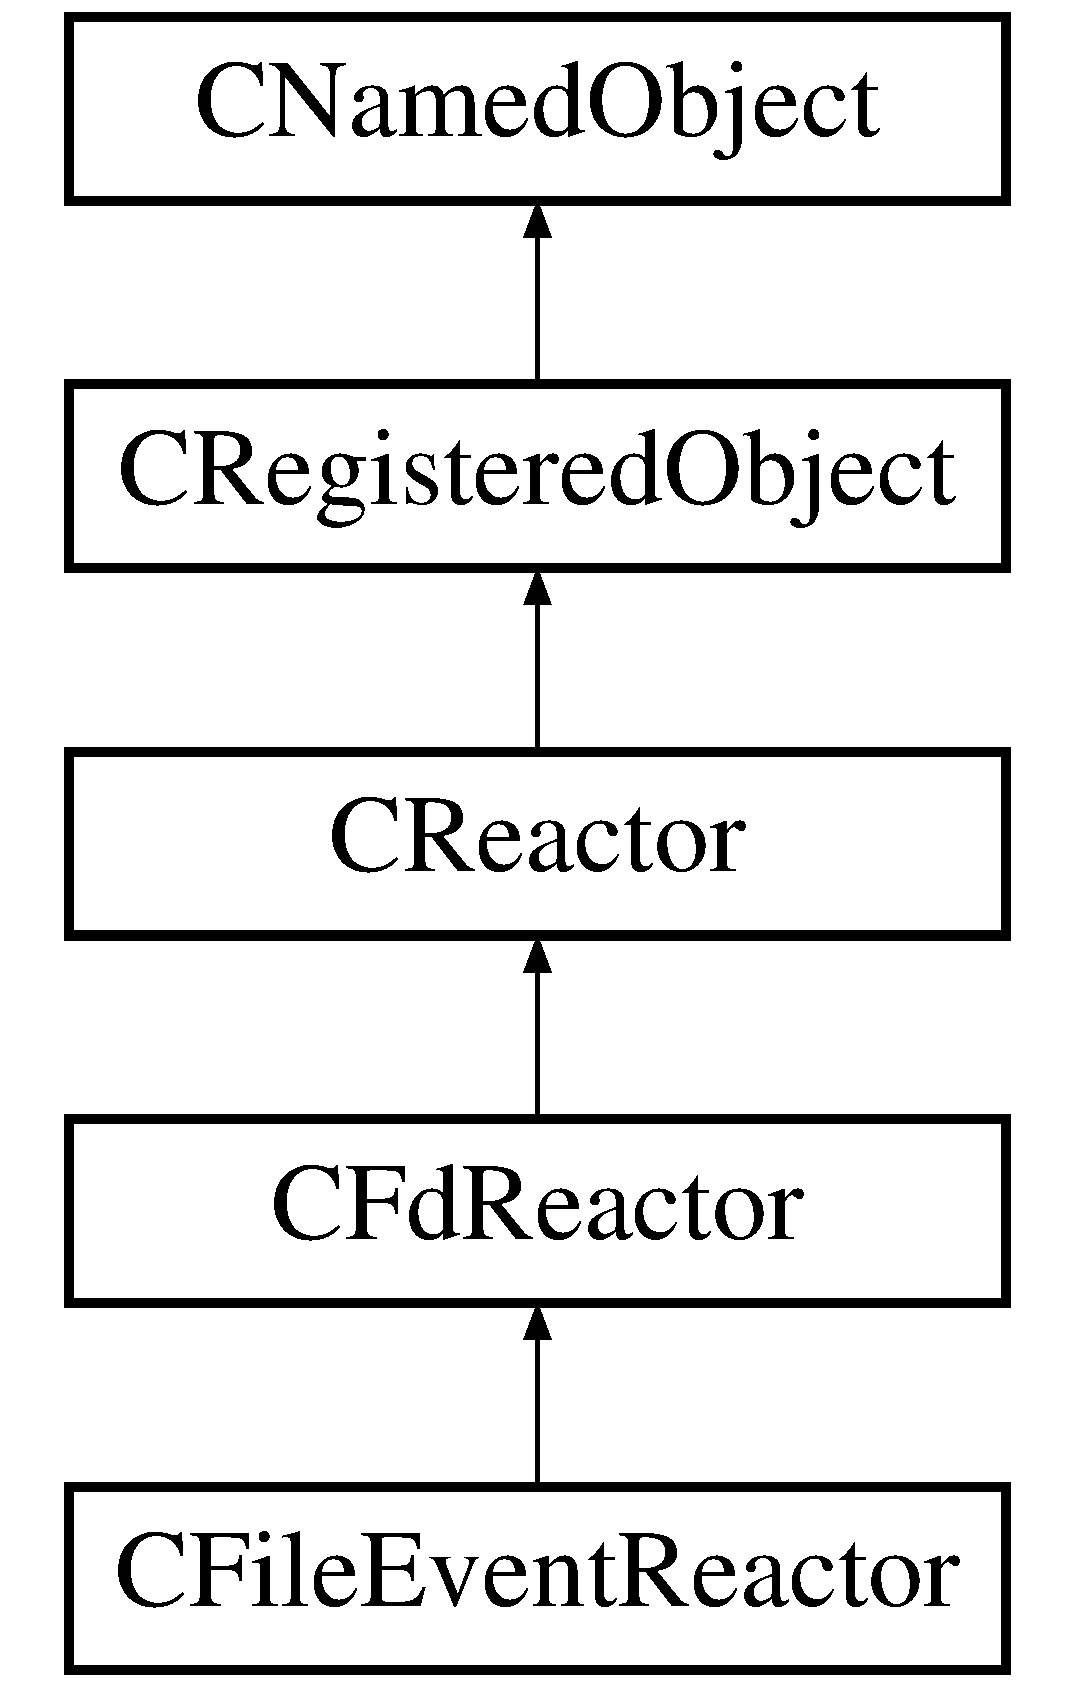
\includegraphics[height=5cm]{classCFileEvent_1_1CFileEventReactor}
\end{center}
\end{figure}
\subsection*{Public Methods}
\begin{CompactItemize}
\item 
{\bf CFile\-Event\-Reactor} (const string \&r\-Name, {\bf CFile\-Event} \&r\-Owner)
\item 
{\bf $\sim$CFile\-Event\-Reactor} ()
\item 
virtual void {\bf On\-Readable} ({\bf CFd\-Monitor} \&r\-Monitor, int fd)
\item 
virtual void {\bf On\-Writable} ({\bf CFd\-Monitor} \&r\-Monitor, int fd)
\item 
virtual void {\bf On\-Exception} ({\bf CFd\-Monitor} \&r\-Monitor, int fd)
\item 
virtual void {\bf On\-Timeout} ({\bf CEvent\-Monitor} \&r\-Monitor)
\end{CompactItemize}
\subsection*{Private Attributes}
\begin{CompactItemize}
\item 
{\bf CFile\-Event} \& {\bf m\_\-r\-Owner}
\begin{CompactList}\small\item\em Owner of us.\item\end{CompactList}\end{CompactItemize}


\subsection{Detailed Description}
This is an internal class which is automatically used as the  Reactor for File events. About the only thing it does is call back to the file event. 



Definition at line 342 of file CFile\-Event.h.

\subsection{Constructor \& Destructor Documentation}
\index{CFileEvent::CFileEventReactor@{CFile\-Event::CFile\-Event\-Reactor}!CFileEventReactor@{CFileEventReactor}}
\index{CFileEventReactor@{CFileEventReactor}!CFileEvent::CFileEventReactor@{CFile\-Event::CFile\-Event\-Reactor}}
\subsubsection{\setlength{\rightskip}{0pt plus 5cm}CFile\-Event\-Reactor::CFile\-Event\-Reactor (const string \& {\em r\-Name}, {\bf CFile\-Event} \& {\em r\-Owner})}\label{classCFileEvent_1_1CFileEventReactor_a0}


Constructor for {\bf CFile\-Event\-Reactor} {\rm (p.\,\pageref{classCFileEvent_1_1CFileEventReactor})}: Constructs the reactor by \begin{CompactItemize}
\item 
Calling the base class constructor ({\bf CReactor}() {\rm (p.\,\pageref{classCReactor_a0})}).\item 
Initializing m\_\-r\-Owner to the event which is instantiating us.\item 
Calling {\bf Append\-Class\-Info}() {\rm (p.\,\pageref{classCNamedObject_b2})} so that our place in the class hierarchy is well defined.\end{CompactItemize}
\begin{Desc}
\item[Parameters: ]\par
\begin{description}
\item[{\em 
r\-Name}]- Reference to the name given to this reactor. \item[{\em 
r\-Owner}]- Reference to the owning event. \end{description}
\end{Desc}


Definition at line 324 of file CFile\-Event.cpp.

References CNamed\-Object::Append\-Class\-Info().\index{CFileEvent::CFileEventReactor@{CFile\-Event::CFile\-Event\-Reactor}!~CFileEventReactor@{$\sim$CFileEventReactor}}
\index{~CFileEventReactor@{$\sim$CFileEventReactor}!CFileEvent::CFileEventReactor@{CFile\-Event::CFile\-Event\-Reactor}}
\subsubsection{\setlength{\rightskip}{0pt plus 5cm}CFile\-Event\-Reactor::$\sim$CFile\-Event\-Reactor ()\hspace{0.3cm}{\tt  [inline]}}\label{classCFileEvent_1_1CFileEventReactor_a1}




Definition at line 347 of file CFile\-Event.h.

\subsection{Member Function Documentation}
\index{CFileEvent::CFileEventReactor@{CFile\-Event::CFile\-Event\-Reactor}!OnException@{OnException}}
\index{OnException@{OnException}!CFileEvent::CFileEventReactor@{CFile\-Event::CFile\-Event\-Reactor}}
\subsubsection{\setlength{\rightskip}{0pt plus 5cm}void CFile\-Event\-Reactor::On\-Exception ({\bf CFd\-Monitor} \& {\em r\-Monitor}, int {\em fd})\hspace{0.3cm}{\tt  [virtual]}}\label{classCFileEvent_1_1CFileEventReactor_a4}


Called when an exceptional condition is encountered on a file. We create an iostream and bounce the call back to m\_\-r\-Owner's On\-Exception. This  creates the look and feel of a monolithic Event class. 

Reimplemented from {\bf CFd\-Reactor} {\rm (p.\,\pageref{classCFdReactor_a8})}.

Definition at line 371 of file CFile\-Event.cpp.

References CFile\-Event\-Reactor::m\_\-r\-Owner, and CFile\-Event::On\-Exception().\index{CFileEvent::CFileEventReactor@{CFile\-Event::CFile\-Event\-Reactor}!OnReadable@{OnReadable}}
\index{OnReadable@{OnReadable}!CFileEvent::CFileEventReactor@{CFile\-Event::CFile\-Event\-Reactor}}
\subsubsection{\setlength{\rightskip}{0pt plus 5cm}void CFile\-Event\-Reactor::On\-Readable ({\bf CFd\-Monitor} \& {\em r\-Monitor}, int {\em fd})\hspace{0.3cm}{\tt  [virtual]}}\label{classCFileEvent_1_1CFileEventReactor_a2}


Called whenever the file becomes readable. We create an istream for the file, and call back to m\_\-r\-Owner's On\-Readable member. This all makes the Event seem like a monolithic unit to the user.... They just subclass it, open a file in an appropriate way and poof.\begin{Desc}
\item[arm r\-Monitor - Refers to the monitor on the file (unused).]\par
 \end{Desc}
\begin{Desc}
\item[Parameters: ]\par
\begin{description}
\item[{\em 
fd}]- File descriptor open on the file. \end{description}
\end{Desc}


Reimplemented from {\bf CFd\-Reactor} {\rm (p.\,\pageref{classCFdReactor_a6})}.

Definition at line 342 of file CFile\-Event.cpp.

References CFile\-Event\-Reactor::m\_\-r\-Owner, and CFile\-Event::On\-Readable().\index{CFileEvent::CFileEventReactor@{CFile\-Event::CFile\-Event\-Reactor}!OnTimeout@{OnTimeout}}
\index{OnTimeout@{OnTimeout}!CFileEvent::CFileEventReactor@{CFile\-Event::CFile\-Event\-Reactor}}
\subsubsection{\setlength{\rightskip}{0pt plus 5cm}void CFile\-Event\-Reactor::On\-Timeout ({\bf CEvent\-Monitor} \& {\em r\-Monitor})\hspace{0.3cm}{\tt  [virtual]}}\label{classCFileEvent_1_1CFileEventReactor_a5}


Called when a wait on the file event times out. \begin{Desc}
\item[Parameters: ]\par
\begin{description}
\item[{\em 
r\-Monitor}]-referens to the event monitor. \end{description}
\end{Desc}


Reimplemented from {\bf CReactor} {\rm (p.\,\pageref{classCReactor_a8})}.

Definition at line 383 of file CFile\-Event.cpp.

References CFile\-Event::get\-Fd(), CFile\-Event\-Reactor::m\_\-r\-Owner, and CFile\-Event::On\-Timeout().\index{CFileEvent::CFileEventReactor@{CFile\-Event::CFile\-Event\-Reactor}!OnWritable@{OnWritable}}
\index{OnWritable@{OnWritable}!CFileEvent::CFileEventReactor@{CFile\-Event::CFile\-Event\-Reactor}}
\subsubsection{\setlength{\rightskip}{0pt plus 5cm}void CFile\-Event\-Reactor::On\-Writable ({\bf CFd\-Monitor} \& {\em r\-Monitor}, int {\em fd})\hspace{0.3cm}{\tt  [virtual]}}\label{classCFileEvent_1_1CFileEventReactor_a3}


Called when a file descriptor becomes writable. We just create a stream and bounce the call back to the {\bf CFile\-Event} {\rm (p.\,\pageref{classCFileEvent})}'s On\-Writable member. This presents a monolithic look and feel to the end user of this library.\begin{Desc}
\item[Parameters: ]\par
\begin{description}
\item[{\em 
r\-Monitor}]- The file monitor which declared the event.(unused) \item[{\em 
fd}]- The file id which is now writable  (constructs the ostream) \end{description}
\end{Desc}


Reimplemented from {\bf CFd\-Reactor} {\rm (p.\,\pageref{classCFdReactor_a7})}.

Definition at line 360 of file CFile\-Event.cpp.

References CFile\-Event\-Reactor::m\_\-r\-Owner, and CFile\-Event::On\-Writable().

\subsection{Member Data Documentation}
\index{CFileEvent::CFileEventReactor@{CFile\-Event::CFile\-Event\-Reactor}!m_rOwner@{m\_\-rOwner}}
\index{m_rOwner@{m\_\-rOwner}!CFileEvent::CFileEventReactor@{CFile\-Event::CFile\-Event\-Reactor}}
\subsubsection{\setlength{\rightskip}{0pt plus 5cm}{\bf CFile\-Event}\& CFile\-Event\-Reactor::m\_\-r\-Owner\hspace{0.3cm}{\tt  [private]}}\label{classCFileEvent_1_1CFileEventReactor_o0}


Owner of us.



Definition at line 344 of file CFile\-Event.h.

Referenced by CFile\-Event\-Reactor::On\-Exception(), CFile\-Event\-Reactor::On\-Readable(), CFile\-Event\-Reactor::On\-Timeout(), and CFile\-Event\-Reactor::On\-Writable().

The documentation for this class was generated from the following files:\begin{CompactItemize}
\item 
{\bf CFile\-Event.cpp}\item 
{\bf CFile\-Event.h}\end{CompactItemize}

\section{Generic\_\-List$<$ T $>$  Class Template Reference}
\label{classGeneric__List}\index{Generic_List@{Generic\_\-List}}
{\tt \#include $<$XMWlist.h$>$}

\subsection*{Public Methods}
\begin{CompactItemize}
\item 
{\bf Generic\_\-List} (int size=LIST\_\-DEFAULT\_\-SIZE)
\item 
{\bf $\sim$Generic\_\-List} ()
\item 
int {\bf Add} (T $\ast$item)
\item 
void {\bf Init\-Iteration} (int loc=0)
\item 
int {\bf Exists} ()
\item 
T $\ast$ {\bf Next} ()
\item 
int {\bf Index} ()
\item 
void {\bf Remove} (int idx)
\end{CompactItemize}
\subsection*{Protected Attributes}
\begin{CompactItemize}
\item 
int {\bf index}
\item 
int {\bf num\_\-entries}
\item 
int {\bf max\_\-entries}
\item 
T $\ast$$\ast$ {\bf entries}
\end{CompactItemize}
\subsubsection*{template$<$class T$>$ class Generic\_\-List$<$ T $>$}



\subsection{Constructor \& Destructor Documentation}
\index{Generic_List@{Generic\_\-List}!Generic_List@{Generic\_\-List}}
\index{Generic_List@{Generic\_\-List}!Generic_List@{Generic\_\-List}}
\subsubsection{\setlength{\rightskip}{0pt plus 5cm}template$<$class T$>$ Generic\_\-List$<$ T $>$::Generic\_\-List (int {\em size} = LIST\_\-DEFAULT\_\-SIZE)\hspace{0.3cm}{\tt  [inline]}}\label{classGeneric__List_a0}




Definition at line 320 of file XMWlist.h.\index{Generic_List@{Generic\_\-List}!~Generic_List@{$\sim$Generic\_\-List}}
\index{~Generic_List@{$\sim$Generic\_\-List}!Generic_List@{Generic\_\-List}}
\subsubsection{\setlength{\rightskip}{0pt plus 5cm}template$<$class T$>$ Generic\_\-List$<$ T $>$::$\sim$Generic\_\-List ()\hspace{0.3cm}{\tt  [inline]}}\label{classGeneric__List_a1}




Definition at line 330 of file XMWlist.h.

\subsection{Member Function Documentation}
\index{Generic_List@{Generic\_\-List}!Add@{Add}}
\index{Add@{Add}!Generic_List@{Generic\_\-List}}
\subsubsection{\setlength{\rightskip}{0pt plus 5cm}template$<$class T$>$ int Generic\_\-List$<$ T $>$::Add (T $\ast$ {\em item})\hspace{0.3cm}{\tt  [inline]}}\label{classGeneric__List_a2}




Definition at line 336 of file XMWlist.h.\index{Generic_List@{Generic\_\-List}!Exists@{Exists}}
\index{Exists@{Exists}!Generic_List@{Generic\_\-List}}
\subsubsection{\setlength{\rightskip}{0pt plus 5cm}template$<$class T$>$ int Generic\_\-List$<$ T $>$::Exists ()\hspace{0.3cm}{\tt  [inline]}}\label{classGeneric__List_a4}




Definition at line 349 of file XMWlist.h.\index{Generic_List@{Generic\_\-List}!Index@{Index}}
\index{Index@{Index}!Generic_List@{Generic\_\-List}}
\subsubsection{\setlength{\rightskip}{0pt plus 5cm}template$<$class T$>$ int Generic\_\-List$<$ T $>$::Index ()\hspace{0.3cm}{\tt  [inline]}}\label{classGeneric__List_a6}




Definition at line 361 of file XMWlist.h.\index{Generic_List@{Generic\_\-List}!InitIteration@{InitIteration}}
\index{InitIteration@{InitIteration}!Generic_List@{Generic\_\-List}}
\subsubsection{\setlength{\rightskip}{0pt plus 5cm}template$<$class T$>$ void Generic\_\-List$<$ T $>$::Init\-Iteration (int {\em loc} = 0)\hspace{0.3cm}{\tt  [inline]}}\label{classGeneric__List_a3}




Definition at line 346 of file XMWlist.h.\index{Generic_List@{Generic\_\-List}!Next@{Next}}
\index{Next@{Next}!Generic_List@{Generic\_\-List}}
\subsubsection{\setlength{\rightskip}{0pt plus 5cm}template$<$class T$>$ T$\ast$ Generic\_\-List$<$ T $>$::Next ()\hspace{0.3cm}{\tt  [inline]}}\label{classGeneric__List_a5}




Definition at line 352 of file XMWlist.h.\index{Generic_List@{Generic\_\-List}!Remove@{Remove}}
\index{Remove@{Remove}!Generic_List@{Generic\_\-List}}
\subsubsection{\setlength{\rightskip}{0pt plus 5cm}template$<$class T$>$ void Generic\_\-List$<$ T $>$::Remove (int {\em idx})\hspace{0.3cm}{\tt  [inline]}}\label{classGeneric__List_a7}




Definition at line 364 of file XMWlist.h.

\subsection{Member Data Documentation}
\index{Generic_List@{Generic\_\-List}!entries@{entries}}
\index{entries@{entries}!Generic_List@{Generic\_\-List}}
\subsubsection{\setlength{\rightskip}{0pt plus 5cm}template$<$class T$>$ T$\ast$$\ast$ Generic\_\-List$<$ T $>$::entries\hspace{0.3cm}{\tt  [protected]}}\label{classGeneric__List_n3}




Definition at line 314 of file XMWlist.h.

Referenced by Generic\_\-List$<$ XMWidget $>$::Add(), Generic\_\-List$<$ XMWidget $>$::Generic\_\-List(), Generic\_\-List$<$ XMWidget $>$::Next(), Generic\_\-List$<$ XMWidget $>$::Remove(), and Generic\_\-List$<$ XMWidget $>$::$\sim$Generic\_\-List().\index{Generic_List@{Generic\_\-List}!index@{index}}
\index{index@{index}!Generic_List@{Generic\_\-List}}
\subsubsection{\setlength{\rightskip}{0pt plus 5cm}template$<$class T$>$ int Generic\_\-List$<$ T $>$::index\hspace{0.3cm}{\tt  [protected]}}\label{classGeneric__List_n0}




Definition at line 311 of file XMWlist.h.

Referenced by Generic\_\-List$<$ XMWidget $>$::Exists(), Generic\_\-List$<$ XMWidget $>$::Generic\_\-List(), Generic\_\-List$<$ XMWidget $>$::Index(), Generic\_\-List$<$ XMWidget $>$::Init\-Iteration(), and Generic\_\-List$<$ XMWidget $>$::Next().\index{Generic_List@{Generic\_\-List}!max_entries@{max\_\-entries}}
\index{max_entries@{max\_\-entries}!Generic_List@{Generic\_\-List}}
\subsubsection{\setlength{\rightskip}{0pt plus 5cm}template$<$class T$>$ int Generic\_\-List$<$ T $>$::max\_\-entries\hspace{0.3cm}{\tt  [protected]}}\label{classGeneric__List_n2}




Definition at line 313 of file XMWlist.h.

Referenced by Generic\_\-List$<$ XMWidget $>$::Add(), and Generic\_\-List$<$ XMWidget $>$::Generic\_\-List().\index{Generic_List@{Generic\_\-List}!num_entries@{num\_\-entries}}
\index{num_entries@{num\_\-entries}!Generic_List@{Generic\_\-List}}
\subsubsection{\setlength{\rightskip}{0pt plus 5cm}template$<$class T$>$ int Generic\_\-List$<$ T $>$::num\_\-entries\hspace{0.3cm}{\tt  [protected]}}\label{classGeneric__List_n1}




Definition at line 312 of file XMWlist.h.

Referenced by Generic\_\-List$<$ XMWidget $>$::Add(), Generic\_\-List$<$ XMWidget $>$::Exists(), Generic\_\-List$<$ XMWidget $>$::Generic\_\-List(), Generic\_\-List$<$ XMWidget $>$::Next(), and Generic\_\-List$<$ XMWidget $>$::Remove().

The documentation for this class was generated from the following file:\begin{CompactItemize}
\item 
{\bf XMWlist.h}\end{CompactItemize}

\section{CIncompatible\-Monitor  Class Reference}
\label{classCIncompatibleMonitor}\index{CIncompatibleMonitor@{CIncompatible\-Monitor}}
{\tt \#include $<$CIncompatible\-Monitor.h$>$}

Inheritance diagram for CIncompatible\-Monitor::\begin{figure}[H]
\begin{center}
\leavevmode
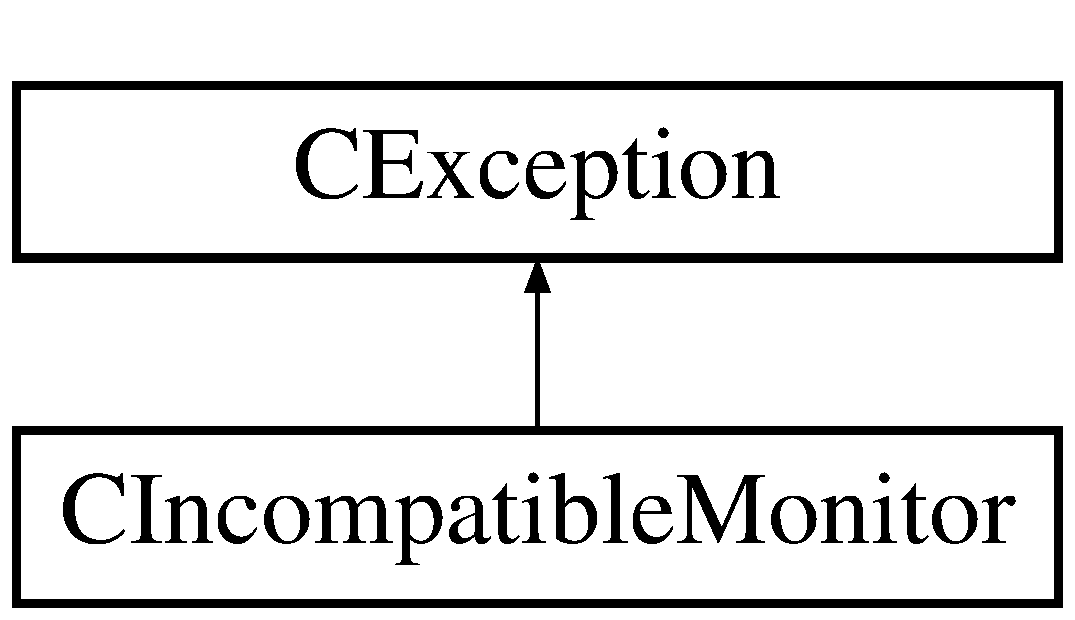
\includegraphics[height=2cm]{classCIncompatibleMonitor}
\end{center}
\end{figure}
\subsection*{Public Methods}
\begin{CompactItemize}
\item 
{\bf CIncompatible\-Monitor} ({\bf CEvent\-Monitor} \&r\-Monitor, const char $\ast$p\-Doing)
\item 
{\bf CIncompatible\-Monitor} (const CIncompatible\-Monitor \&rhs)
\item 
virtual {\bf $\sim$CIncompatible\-Monitor} ()
\item 
CIncompatible\-Monitor \& {\bf operator=} (const CIncompatible\-Monitor \&rhs)
\item 
int {\bf operator==} (const CIncompatible\-Monitor \&rhs)
\item 
string {\bf get\-Monitor\-Description} () const
\item 
void {\bf set\-Monitor\-Description} (const string \&rnew)
\item 
virtual const char $\ast$ {\bf Reason\-Text} () const
\end{CompactItemize}
\subsection*{Private Attributes}
\begin{CompactItemize}
\item 
string {\bf m\_\-Monitor\-Description}
\item 
string {\bf m\_\-Reason}
\end{CompactItemize}


\subsection{Detailed Description}
Encapsulates exceptions thrown when a reactor sense that it has been attached to an incompatible event monitor. The exception is capable of returning textual string information about the type of the monitor received and what the reactor was doing when it threw the exception. 



Definition at line 307 of file CIncompatible\-Monitor.h.

\subsection{Constructor \& Destructor Documentation}
\index{CIncompatibleMonitor@{CIncompatible\-Monitor}!CIncompatibleMonitor@{CIncompatibleMonitor}}
\index{CIncompatibleMonitor@{CIncompatibleMonitor}!CIncompatibleMonitor@{CIncompatible\-Monitor}}
\subsubsection{\setlength{\rightskip}{0pt plus 5cm}CIncompatible\-Monitor::CIncompatible\-Monitor ({\bf CEvent\-Monitor} \& {\em r\-Monitor}, const char $\ast$ {\em p\-Doing})}\label{classCIncompatibleMonitor_a0}


\char`\"{}Normal\char`\"{} Constructor. Constructs an incompatible exception object just prior to throwing it. Information from the monitor is stored as is information about what was happening in the system at the time the exception was constructed:\begin{Desc}
\item[Parameters: ]\par
\begin{description}
\item[{\em 
r\-Monitor}]- The monitor which was not compatible with the Reactor that detected the problem. \item[{\em 
p\-Doing}]- Text string describing what the program was attempting to do when the incompatibility was detected. \end{description}
\end{Desc}


Definition at line 306 of file CIncompatible\-Monitor.cpp.\index{CIncompatibleMonitor@{CIncompatible\-Monitor}!CIncompatibleMonitor@{CIncompatibleMonitor}}
\index{CIncompatibleMonitor@{CIncompatibleMonitor}!CIncompatibleMonitor@{CIncompatible\-Monitor}}
\subsubsection{\setlength{\rightskip}{0pt plus 5cm}CIncompatible\-Monitor::CIncompatible\-Monitor (const CIncompatible\-Monitor \& {\em rhs})}\label{classCIncompatibleMonitor_a1}


Copy constructor. Used by the compiler construct temporary objects or  alternatively, and more usually for this class to build a 'scope safe' copy of the exception which can be saved and passed to catch handlers. \begin{Desc}
\item[Parameters: ]\par
\begin{description}
\item[{\em 
rhs}]- the reference object being copy constructed. \end{description}
\end{Desc}


Definition at line 320 of file CIncompatible\-Monitor.cpp.\index{CIncompatibleMonitor@{CIncompatible\-Monitor}!~CIncompatibleMonitor@{$\sim$CIncompatibleMonitor}}
\index{~CIncompatibleMonitor@{$\sim$CIncompatibleMonitor}!CIncompatibleMonitor@{CIncompatible\-Monitor}}
\subsubsection{\setlength{\rightskip}{0pt plus 5cm}virtual CIncompatible\-Monitor::$\sim$CIncompatible\-Monitor ()\hspace{0.3cm}{\tt  [inline, virtual]}}\label{classCIncompatibleMonitor_a2}




Definition at line 318 of file CIncompatible\-Monitor.h.

\subsection{Member Function Documentation}
\index{CIncompatibleMonitor@{CIncompatible\-Monitor}!getMonitorDescription@{getMonitorDescription}}
\index{getMonitorDescription@{getMonitorDescription}!CIncompatibleMonitor@{CIncompatible\-Monitor}}
\subsubsection{\setlength{\rightskip}{0pt plus 5cm}string CIncompatible\-Monitor::get\-Monitor\-Description () const\hspace{0.3cm}{\tt  [inline]}}\label{classCIncompatibleMonitor_a5}




Definition at line 325 of file CIncompatible\-Monitor.h.

References m\_\-Monitor\-Description.\index{CIncompatibleMonitor@{CIncompatible\-Monitor}!operator=@{operator=}}
\index{operator=@{operator=}!CIncompatibleMonitor@{CIncompatible\-Monitor}}
\subsubsection{\setlength{\rightskip}{0pt plus 5cm}CIncompatible\-Monitor \& CIncompatible\-Monitor::operator= (const CIncompatible\-Monitor \& {\em rhs})}\label{classCIncompatibleMonitor_a3}


Assignment operator. .much like copy construction except:\begin{CompactItemize}
\item 
We gaurd against self assignment problems.\item 
We are already a fully constructed object in our own right.\item 
We return a refereince to $\ast$this.\end{CompactItemize}
\begin{Desc}
\item[Parameters: ]\par
\begin{description}
\item[{\em 
rhs}]- the object being assigned to us. \end{description}
\end{Desc}


Definition at line 335 of file CIncompatible\-Monitor.cpp.

References m\_\-Monitor\-Description, and CException::operator=().\index{CIncompatibleMonitor@{CIncompatible\-Monitor}!operator==@{operator==}}
\index{operator==@{operator==}!CIncompatibleMonitor@{CIncompatible\-Monitor}}
\subsubsection{\setlength{\rightskip}{0pt plus 5cm}int CIncompatible\-Monitor::operator== (const CIncompatible\-Monitor \& {\em rhs})}\label{classCIncompatibleMonitor_a4}


Equality comparison. We do base class comparison and compare the monitor description. The m\_\-Reason string is not relevant.\begin{Desc}
\item[Parameters: ]\par
\begin{description}
\item[{\em 
rhs}]- Reference to object we compare ourselves to. \end{description}
\end{Desc}


Definition at line 351 of file CIncompatible\-Monitor.cpp.

References m\_\-Monitor\-Description, and CException::operator==().\index{CIncompatibleMonitor@{CIncompatible\-Monitor}!ReasonText@{ReasonText}}
\index{ReasonText@{ReasonText}!CIncompatibleMonitor@{CIncompatible\-Monitor}}
\subsubsection{\setlength{\rightskip}{0pt plus 5cm}const char $\ast$ CIncompatible\-Monitor::Reason\-Text () const\hspace{0.3cm}{\tt  [virtual]}}\label{classCIncompatibleMonitor_a7}


Returns a description of why the exception is being thrown. This is of the form: Incompatible Event monitor found: \char`\"{}monitor description\char`\"{}, while: Doing\char`\"{} 

Reimplemented from {\bf CException} {\rm (p.\,\pageref{classCException_a8})}.

Definition at line 363 of file CIncompatible\-Monitor.cpp.

References m\_\-Monitor\-Description, m\_\-Reason, and CException::Was\-Doing().\index{CIncompatibleMonitor@{CIncompatible\-Monitor}!setMonitorDescription@{setMonitorDescription}}
\index{setMonitorDescription@{setMonitorDescription}!CIncompatibleMonitor@{CIncompatible\-Monitor}}
\subsubsection{\setlength{\rightskip}{0pt plus 5cm}void CIncompatible\-Monitor::set\-Monitor\-Description (const string \& {\em rnew})\hspace{0.3cm}{\tt  [inline]}}\label{classCIncompatibleMonitor_a6}




Definition at line 331 of file CIncompatible\-Monitor.h.

References m\_\-Monitor\-Description.

\subsection{Member Data Documentation}
\index{CIncompatibleMonitor@{CIncompatible\-Monitor}!m_MonitorDescription@{m\_\-MonitorDescription}}
\index{m_MonitorDescription@{m\_\-MonitorDescription}!CIncompatibleMonitor@{CIncompatible\-Monitor}}
\subsubsection{\setlength{\rightskip}{0pt plus 5cm}string CIncompatible\-Monitor::m\_\-Monitor\-Description\hspace{0.3cm}{\tt  [private]}}\label{classCIncompatibleMonitor_o0}




Definition at line 311 of file CIncompatible\-Monitor.h.

Referenced by get\-Monitor\-Description(), operator=(), operator==(), Reason\-Text(), and set\-Monitor\-Description().\index{CIncompatibleMonitor@{CIncompatible\-Monitor}!m_Reason@{m\_\-Reason}}
\index{m_Reason@{m\_\-Reason}!CIncompatibleMonitor@{CIncompatible\-Monitor}}
\subsubsection{\setlength{\rightskip}{0pt plus 5cm}string CIncompatible\-Monitor::m\_\-Reason\hspace{0.3cm}{\tt  [private]}}\label{classCIncompatibleMonitor_o1}




Definition at line 312 of file CIncompatible\-Monitor.h.

Referenced by Reason\-Text().

The documentation for this class was generated from the following files:\begin{CompactItemize}
\item 
{\bf CIncompatible\-Monitor.h}\item 
{\bf CIncompatible\-Monitor.cpp}\end{CompactItemize}

\section{CInit\-Binding  Class Reference}
\label{classCInitBinding}\index{CInitBinding@{CInit\-Binding}}
\subsection*{Public Methods}
\begin{CompactItemize}
\item 
{\bf CInit\-Binding} ({\bf CTCLInterpreter} \&r\-Interp)
\item 
void {\bf operator()} ({\bf CType\-Free\-Binding} $\ast$p\-Binding)
\end{CompactItemize}
\subsection*{Private Attributes}
\begin{CompactItemize}
\item 
{\bf CTCLInterpreter} \& {\bf m\_\-r\-Interp}
\end{CompactItemize}


\subsection{Constructor \& Destructor Documentation}
\index{CInitBinding@{CInit\-Binding}!CInitBinding@{CInitBinding}}
\index{CInitBinding@{CInitBinding}!CInitBinding@{CInit\-Binding}}
\subsubsection{\setlength{\rightskip}{0pt plus 5cm}CInit\-Binding::CInit\-Binding ({\bf CTCLInterpreter} \& {\em r\-Interp})\hspace{0.3cm}{\tt  [inline]}}\label{classCInitBinding_a0}




Definition at line 311 of file CConfiguration\-Manager.cpp.

\subsection{Member Function Documentation}
\index{CInitBinding@{CInit\-Binding}!operator()@{operator()}}
\index{operator()@{operator()}!CInitBinding@{CInit\-Binding}}
\subsubsection{\setlength{\rightskip}{0pt plus 5cm}void CInit\-Binding::operator() ({\bf CType\-Free\-Binding} $\ast$ {\em p\-Binding})\hspace{0.3cm}{\tt  [inline]}}\label{classCInitBinding_a1}




Definition at line 312 of file CConfiguration\-Manager.cpp.

References CType\-Free\-Binding::Init\-Bindings().

\subsection{Member Data Documentation}
\index{CInitBinding@{CInit\-Binding}!m_rInterp@{m\_\-rInterp}}
\index{m_rInterp@{m\_\-rInterp}!CInitBinding@{CInit\-Binding}}
\subsubsection{\setlength{\rightskip}{0pt plus 5cm}{\bf CTCLInterpreter}\& CInit\-Binding::m\_\-r\-Interp\hspace{0.3cm}{\tt  [private]}}\label{classCInitBinding_o0}




Definition at line 309 of file CConfiguration\-Manager.cpp.

The documentation for this class was generated from the following file:\begin{CompactItemize}
\item 
{\bf CConfiguration\-Manager.cpp}\end{CompactItemize}

\section{CInterpreter\-Startup  Class Reference}
\label{classCInterpreterStartup}\index{CInterpreterStartup@{CInterpreter\-Startup}}
{\tt \#include $<$CInterpreter\-Startup.h$>$}

Inheritance diagram for CInterpreter\-Startup::\begin{figure}[H]
\begin{center}
\leavevmode
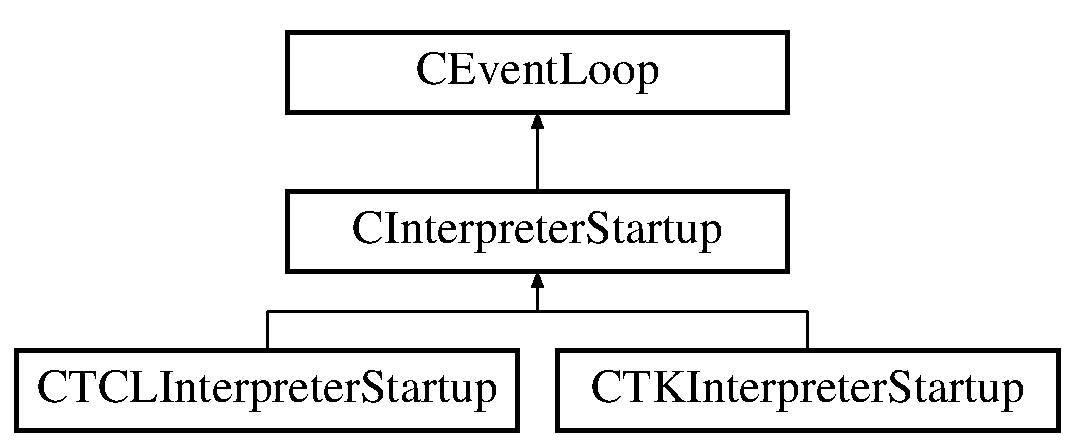
\includegraphics[height=3cm]{classCInterpreterStartup}
\end{center}
\end{figure}
\subsection*{Public Methods}
\begin{CompactItemize}
\item 
{\bf CInterpreter\-Startup} ()
\begin{CompactList}\small\item\em Nulls out the interpreter and sync command pointers.\item\end{CompactList}\item 
virtual {\bf $\sim$CInterpreter\-Startup} ()
\item 
{\bf CTCLInterpreter} $\ast$ {\bf get\-Interpreter} ()
\begin{CompactList}\small\item\em Return a pointer to the interpreter object.\item\end{CompactList}\item 
{\bf CTCLInterpreter} \& {\bf Interp} ()
\end{CompactItemize}
\subsection*{Protected Methods}
\begin{CompactItemize}
\item 
virtual void {\bf On\-Initialize} (int argc, char $\ast$$\ast$Argv)
\item 
virtual void {\bf Register\-Extensions} ()
\item 
void {\bf set\-Interpreter} ({\bf CTCLInterpreter} $\ast$p\-Interp)
\begin{CompactList}\small\item\em Set the interpreter object:.\item\end{CompactList}\end{CompactItemize}
\subsection*{Private Methods}
\begin{CompactItemize}
\item 
int {\bf operator()} (int argc, char $\ast$$\ast$argv)=0
\item 
{\bf CInterpreter\-Startup} (const CInterpreter\-Startup \&a\-CInterpreter\-Startup)
\begin{CompactList}\small\item\em Copy Constructor is forbidden, private, unimplemented.\item\end{CompactList}\item 
CInterpreter\-Startup \& {\bf operator=} (const CInterpreter\-Startup \&a\-CInterpreter\-Startup)
\begin{CompactList}\small\item\em Assignment is forbidden, private, unimplemented.\item\end{CompactList}\item 
int {\bf operator==} (const CInterpreter\-Startup \&a\-CInterpreter\-Startup) const
\begin{CompactList}\small\item\em Operator== Equality Operator forbidden, private, unimplemented.\item\end{CompactList}\end{CompactItemize}
\subsection*{Private Attributes}
\begin{CompactItemize}
\item 
{\bf CTCLInterpreter} $\ast$ {\bf m\_\-p\-Interp}
\item 
{\bf CTCLSynchronize\-Command} $\ast$ {\bf m\_\-p\-Sync\-Command}
\end{CompactItemize}


\subsection{Detailed Description}
Encapsulates interfaces for starting up  TCL based interpreter event loops. The TCL interpreter executes within a thread. Adding a command to the interpreter should be done by subclassing {\bf CDAQTCLProcessor} {\rm (p.\,\pageref{classCDAQTCLProcessor})}, instantiating an object for that class, and registring it on the current interpreter. It is important that DAQTCLProcessor objects be used rather than TCLProcessor objects since DAQTCLProcessor is thread-aware and will therefore synchronize its action through the application's global mutex. 



Definition at line 315 of file CInterpreter\-Startup.h.

\subsection{Constructor \& Destructor Documentation}
\index{CInterpreterStartup@{CInterpreter\-Startup}!CInterpreterStartup@{CInterpreterStartup}}
\index{CInterpreterStartup@{CInterpreterStartup}!CInterpreterStartup@{CInterpreter\-Startup}}
\subsubsection{\setlength{\rightskip}{0pt plus 5cm}CInterpreter\-Startup::CInterpreter\-Startup ()}\label{classCInterpreterStartup_a0}


Nulls out the interpreter and sync command pointers.

Encapsulates interfaces for starting up  TCL based interpreter event loops. The TCL interpreter executes within a thread. Adding a command to the interpreter should be done by subclassing {\bf CDAQTCLProcessor} {\rm (p.\,\pageref{classCDAQTCLProcessor})}, instantiating an object for that class, and registring it on the current interpreter. It is important that DAQTCLProcessor objects be used rather than TCLProcessor objects since DAQTCLProcessor is thread-aware and will therefore synchronize its action  through the application's global mutex. 

Definition at line 300 of file CInterpreter\-Startup.cpp.\index{CInterpreterStartup@{CInterpreter\-Startup}!~CInterpreterStartup@{$\sim$CInterpreterStartup}}
\index{~CInterpreterStartup@{$\sim$CInterpreterStartup}!CInterpreterStartup@{CInterpreter\-Startup}}
\subsubsection{\setlength{\rightskip}{0pt plus 5cm}CInterpreter\-Startup::$\sim$CInterpreter\-Startup ()\hspace{0.3cm}{\tt  [virtual]}}\label{classCInterpreterStartup_a1}


The destructor only destroys the sync command. The subclass is responsible for destroying the interpreter which in turn will unregister the sync command 

Definition at line 311 of file CInterpreter\-Startup.cpp.

References m\_\-p\-Sync\-Command.\index{CInterpreterStartup@{CInterpreter\-Startup}!CInterpreterStartup@{CInterpreterStartup}}
\index{CInterpreterStartup@{CInterpreterStartup}!CInterpreterStartup@{CInterpreter\-Startup}}
\subsubsection{\setlength{\rightskip}{0pt plus 5cm}CInterpreter\-Startup::CInterpreter\-Startup (const CInterpreter\-Startup \& {\em a\-CInterpreter\-Startup})\hspace{0.3cm}{\tt  [private]}}\label{classCInterpreterStartup_c1}


Copy Constructor is forbidden, private, unimplemented.



\subsection{Member Function Documentation}
\index{CInterpreterStartup@{CInterpreter\-Startup}!getInterpreter@{getInterpreter}}
\index{getInterpreter@{getInterpreter}!CInterpreterStartup@{CInterpreter\-Startup}}
\subsubsection{\setlength{\rightskip}{0pt plus 5cm}{\bf CTCLInterpreter}$\ast$ CInterpreter\-Startup::get\-Interpreter ()\hspace{0.3cm}{\tt  [inline]}}\label{classCInterpreterStartup_a2}


Return a pointer to the interpreter object.



Definition at line 353 of file CInterpreter\-Startup.h.\index{CInterpreterStartup@{CInterpreter\-Startup}!Interp@{Interp}}
\index{Interp@{Interp}!CInterpreterStartup@{CInterpreter\-Startup}}
\subsubsection{\setlength{\rightskip}{0pt plus 5cm}{\bf CTCLInterpreter}\& CInterpreter\-Startup::Interp ()\hspace{0.3cm}{\tt  [inline]}}\label{classCInterpreterStartup_a3}


Get a reference to the interpreter object: Note that this can fail if there is not yet an interpreter (m\_\-p\-Interp is NULL in that case). 

Definition at line 360 of file CInterpreter\-Startup.h.\index{CInterpreterStartup@{CInterpreter\-Startup}!OnInitialize@{OnInitialize}}
\index{OnInitialize@{OnInitialize}!CInterpreterStartup@{CInterpreter\-Startup}}
\subsubsection{\setlength{\rightskip}{0pt plus 5cm}void CInterpreter\-Startup::On\-Initialize (int {\em argc}, char $\ast$$\ast$ {\em Argv})\hspace{0.3cm}{\tt  [protected, virtual]}}\label{classCInterpreterStartup_b0}


On initialize is called very early in  the execution of the operator() member. It is intended that subclassed interpreters perform early initialization here. At this point an interpreter has not yet been  instantiated. Therefore, you may not perform Tcl/Tk library calls at this  stage.

Default implementation is a no-op. 

Definition at line 332 of file CInterpreter\-Startup.cpp.

Referenced by CTKInterpreter\-Startup::operator()(), and CTCLInterpreter\-Startup::operator()().\index{CInterpreterStartup@{CInterpreter\-Startup}!operator()@{operator()}}
\index{operator()@{operator()}!CInterpreterStartup@{CInterpreter\-Startup}}
\subsubsection{\setlength{\rightskip}{0pt plus 5cm}int CInterpreter\-Startup::operator() (int {\em argc}, char $\ast$$\ast$ {\em argv})\hspace{0.3cm}{\tt  [private, pure virtual]}}\label{classCInterpreterStartup_c0}


This pure virtual member function is expected to start the interpreter and call the other member functions; it is the entry point of the thread. 

Implements {\bf CEvent\-Loop} {\rm (p.\,\pageref{classCEventLoop_c0})}.

Implemented in {\bf CTCLInterpreter\-Startup} {\rm (p.\,\pageref{classCTCLInterpreterStartup_c0})}, and {\bf CTKInterpreter\-Startup} {\rm (p.\,\pageref{classCTKInterpreterStartup_c3})}.\index{CInterpreterStartup@{CInterpreter\-Startup}!operator=@{operator=}}
\index{operator=@{operator=}!CInterpreterStartup@{CInterpreter\-Startup}}
\subsubsection{\setlength{\rightskip}{0pt plus 5cm}CInterpreter\-Startup\& CInterpreter\-Startup::operator= (const CInterpreter\-Startup \& {\em a\-CInterpreter\-Startup})\hspace{0.3cm}{\tt  [private]}}\label{classCInterpreterStartup_c2}


Assignment is forbidden, private, unimplemented.

\index{CInterpreterStartup@{CInterpreter\-Startup}!operator==@{operator==}}
\index{operator==@{operator==}!CInterpreterStartup@{CInterpreter\-Startup}}
\subsubsection{\setlength{\rightskip}{0pt plus 5cm}int CInterpreter\-Startup::operator== (const CInterpreter\-Startup \& {\em a\-CInterpreter\-Startup}) const\hspace{0.3cm}{\tt  [private]}}\label{classCInterpreterStartup_c3}


Operator== Equality Operator forbidden, private, unimplemented.

\index{CInterpreterStartup@{CInterpreter\-Startup}!RegisterExtensions@{RegisterExtensions}}
\index{RegisterExtensions@{RegisterExtensions}!CInterpreterStartup@{CInterpreter\-Startup}}
\subsubsection{\setlength{\rightskip}{0pt plus 5cm}void CInterpreter\-Startup::Register\-Extensions ()\hspace{0.3cm}{\tt  [protected, virtual]}}\label{classCInterpreterStartup_b1}


Concrete subclasses of this class must implement this function. It is expected that all tcl interpreters run in this envrionment will have extensions At this point, an interpreter has been created.

If this is a Tk derived  interpreter, it's not certain that the tk Main window has been created yet however.

Default behavior which should be chained to by subclasses is to register the synch command. This makes available scripts which are synchronized to the application's global mutex. 

Definition at line 355 of file CInterpreter\-Startup.cpp.

References m\_\-p\-Interp, m\_\-p\-Sync\-Command, and CDAQTCLProcessor::Register().

Referenced by CTCLInterpreter\-Startup::Tcl\_\-Init(), and CTKInterpreter\-Startup::Tk\_\-Init().\index{CInterpreterStartup@{CInterpreter\-Startup}!setInterpreter@{setInterpreter}}
\index{setInterpreter@{setInterpreter}!CInterpreterStartup@{CInterpreter\-Startup}}
\subsubsection{\setlength{\rightskip}{0pt plus 5cm}void CInterpreter\-Startup::set\-Interpreter ({\bf CTCLInterpreter} $\ast$ {\em p\-Interp})\hspace{0.3cm}{\tt  [inline, protected]}}\label{classCInterpreterStartup_b2}


Set the interpreter object:.



Definition at line 368 of file CInterpreter\-Startup.h.

Referenced by CTCLInterpreter\-Startup::Tcl\_\-Init(), and CTKInterpreter\-Startup::Tk\_\-Init().

\subsection{Member Data Documentation}
\index{CInterpreterStartup@{CInterpreter\-Startup}!m_pInterp@{m\_\-pInterp}}
\index{m_pInterp@{m\_\-pInterp}!CInterpreterStartup@{CInterpreter\-Startup}}
\subsubsection{\setlength{\rightskip}{0pt plus 5cm}{\bf CTCLInterpreter}$\ast$ CInterpreter\-Startup::m\_\-p\-Interp\hspace{0.3cm}{\tt  [private]}}\label{classCInterpreterStartup_o0}




Definition at line 318 of file CInterpreter\-Startup.h.

Referenced by Register\-Extensions().\index{CInterpreterStartup@{CInterpreter\-Startup}!m_pSyncCommand@{m\_\-pSyncCommand}}
\index{m_pSyncCommand@{m\_\-pSyncCommand}!CInterpreterStartup@{CInterpreter\-Startup}}
\subsubsection{\setlength{\rightskip}{0pt plus 5cm}{\bf CTCLSynchronize\-Command}$\ast$ CInterpreter\-Startup::m\_\-p\-Sync\-Command\hspace{0.3cm}{\tt  [private]}}\label{classCInterpreterStartup_o1}




Definition at line 319 of file CInterpreter\-Startup.h.

Referenced by Register\-Extensions(), and $\sim$CInterpreter\-Startup().

The documentation for this class was generated from the following files:\begin{CompactItemize}
\item 
{\bf CInterpreter\-Startup.h}\item 
{\bf CInterpreter\-Startup.cpp}\end{CompactItemize}

\section{CLink\-Failed\-Exception  Class Reference}
\label{classCLinkFailedException}\index{CLinkFailedException@{CLink\-Failed\-Exception}}
{\tt \#include $<$CLink\-Failed\-Exception.h$>$}

Inheritance diagram for CLink\-Failed\-Exception::\begin{figure}[H]
\begin{center}
\leavevmode
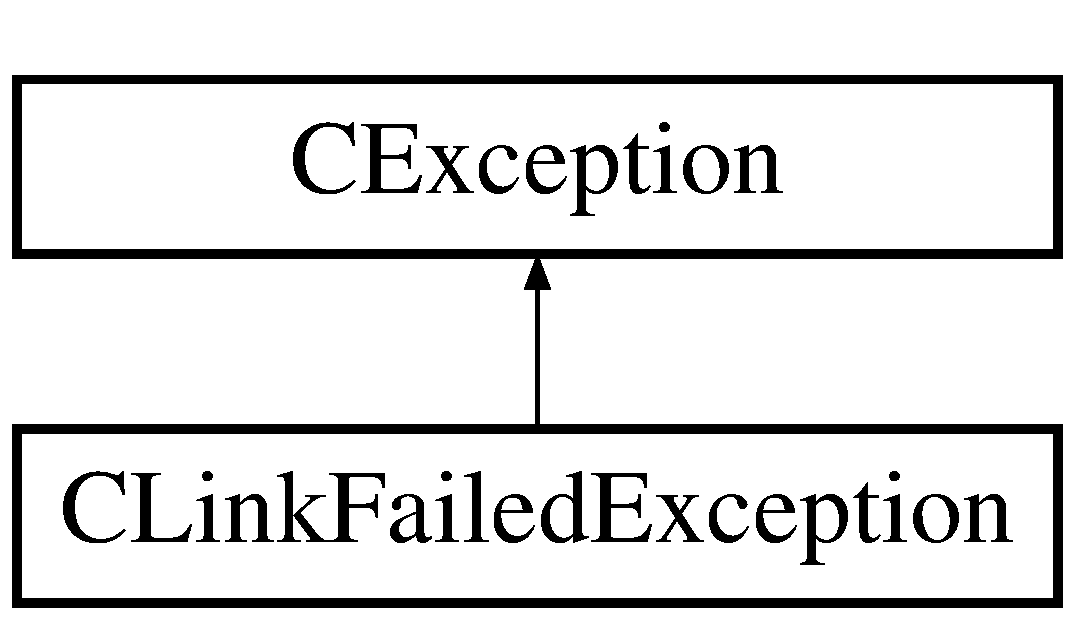
\includegraphics[height=2cm]{classCLinkFailedException}
\end{center}
\end{figure}
\subsection*{Public Methods}
\begin{CompactItemize}
\item 
{\bf CLink\-Failed\-Exception} (const char $\ast$p\-Doing, const char $\ast$p\-Name)
\item 
{\bf CLink\-Failed\-Exception} (const char $\ast$p\-Doing, const string \&r\-Name)
\item 
{\bf CLink\-Failed\-Exception} (const string \&r\-Doing, const char $\ast$p\-Name)
\item 
{\bf CLink\-Failed\-Exception} (const string \&r\-Doing, const string \&r\-Name)
\item 
{\bf CLink\-Failed\-Exception} (const string \&r\-Doing, int n\-Id)
\item 
{\bf CLink\-Failed\-Exception} (const char $\ast$p\-Doing, int n\-Id)
\item 
virtual {\bf $\sim$CLink\-Failed\-Exception} ()
\item 
{\bf CLink\-Failed\-Exception} (const CLink\-Failed\-Exception \&a\-CLink\-Failed\-Exception)
\item 
CLink\-Failed\-Exception {\bf operator=} (const CLink\-Failed\-Exception \&a\-CLink\-Failed\-Exception)
\item 
int {\bf operator==} (const CLink\-Failed\-Exception \&a\-CLink\-Failed\-Exception)
\item 
string {\bf get\-Name} () const
\item 
void {\bf set\-Name} (string am\_\-s\-Name)
\item 
virtual const char $\ast$ {\bf Reason\-Text} () const
\end{CompactItemize}
\subsection*{Protected Methods}
\begin{CompactItemize}
\item 
void {\bf Update\-Reason\-Text} ()
\end{CompactItemize}
\subsection*{Private Attributes}
\begin{CompactItemize}
\item 
string {\bf m\_\-s\-Name}
\item 
int {\bf m\_\-n\-Id}
\item 
bool {\bf m\_\-f\-Name}
\item 
string {\bf m\_\-s\-Reason\-Text}
\end{CompactItemize}


\subsection{Constructor \& Destructor Documentation}
\index{CLinkFailedException@{CLink\-Failed\-Exception}!CLinkFailedException@{CLinkFailedException}}
\index{CLinkFailedException@{CLinkFailedException}!CLinkFailedException@{CLink\-Failed\-Exception}}
\subsubsection{\setlength{\rightskip}{0pt plus 5cm}CLink\-Failed\-Exception::CLink\-Failed\-Exception (const char $\ast$ {\em p\-Doing}, const char $\ast$ {\em p\-Name})\hspace{0.3cm}{\tt  [inline]}}\label{classCLinkFailedException_a0}




Definition at line 301 of file CLink\-Failed\-Exception.h.

References m\_\-f\-Name, m\_\-s\-Name, and Update\-Reason\-Text().\index{CLinkFailedException@{CLink\-Failed\-Exception}!CLinkFailedException@{CLinkFailedException}}
\index{CLinkFailedException@{CLinkFailedException}!CLinkFailedException@{CLink\-Failed\-Exception}}
\subsubsection{\setlength{\rightskip}{0pt plus 5cm}CLink\-Failed\-Exception::CLink\-Failed\-Exception (const char $\ast$ {\em p\-Doing}, const string \& {\em r\-Name})\hspace{0.3cm}{\tt  [inline]}}\label{classCLinkFailedException_a1}




Definition at line 307 of file CLink\-Failed\-Exception.h.

References m\_\-f\-Name, m\_\-s\-Name, and Update\-Reason\-Text().\index{CLinkFailedException@{CLink\-Failed\-Exception}!CLinkFailedException@{CLinkFailedException}}
\index{CLinkFailedException@{CLinkFailedException}!CLinkFailedException@{CLink\-Failed\-Exception}}
\subsubsection{\setlength{\rightskip}{0pt plus 5cm}CLink\-Failed\-Exception::CLink\-Failed\-Exception (const string \& {\em r\-Doing}, const char $\ast$ {\em p\-Name})\hspace{0.3cm}{\tt  [inline]}}\label{classCLinkFailedException_a2}




Definition at line 313 of file CLink\-Failed\-Exception.h.

References m\_\-f\-Name, m\_\-s\-Name, and Update\-Reason\-Text().\index{CLinkFailedException@{CLink\-Failed\-Exception}!CLinkFailedException@{CLinkFailedException}}
\index{CLinkFailedException@{CLinkFailedException}!CLinkFailedException@{CLink\-Failed\-Exception}}
\subsubsection{\setlength{\rightskip}{0pt plus 5cm}CLink\-Failed\-Exception::CLink\-Failed\-Exception (const string \& {\em r\-Doing}, const string \& {\em r\-Name})\hspace{0.3cm}{\tt  [inline]}}\label{classCLinkFailedException_a3}




Definition at line 319 of file CLink\-Failed\-Exception.h.

References m\_\-f\-Name, m\_\-s\-Name, and Update\-Reason\-Text().\index{CLinkFailedException@{CLink\-Failed\-Exception}!CLinkFailedException@{CLinkFailedException}}
\index{CLinkFailedException@{CLinkFailedException}!CLinkFailedException@{CLink\-Failed\-Exception}}
\subsubsection{\setlength{\rightskip}{0pt plus 5cm}CLink\-Failed\-Exception::CLink\-Failed\-Exception (const string \& {\em r\-Doing}, int {\em n\-Id})\hspace{0.3cm}{\tt  [inline]}}\label{classCLinkFailedException_a4}




Definition at line 325 of file CLink\-Failed\-Exception.h.

References m\_\-f\-Name, m\_\-n\-Id, and Update\-Reason\-Text().\index{CLinkFailedException@{CLink\-Failed\-Exception}!CLinkFailedException@{CLinkFailedException}}
\index{CLinkFailedException@{CLinkFailedException}!CLinkFailedException@{CLink\-Failed\-Exception}}
\subsubsection{\setlength{\rightskip}{0pt plus 5cm}CLink\-Failed\-Exception::CLink\-Failed\-Exception (const char $\ast$ {\em p\-Doing}, int {\em n\-Id})\hspace{0.3cm}{\tt  [inline]}}\label{classCLinkFailedException_a5}




Definition at line 331 of file CLink\-Failed\-Exception.h.

References m\_\-f\-Name, m\_\-n\-Id, and Update\-Reason\-Text().\index{CLinkFailedException@{CLink\-Failed\-Exception}!~CLinkFailedException@{$\sim$CLinkFailedException}}
\index{~CLinkFailedException@{$\sim$CLinkFailedException}!CLinkFailedException@{CLink\-Failed\-Exception}}
\subsubsection{\setlength{\rightskip}{0pt plus 5cm}virtual CLink\-Failed\-Exception::$\sim$CLink\-Failed\-Exception ()\hspace{0.3cm}{\tt  [inline, virtual]}}\label{classCLinkFailedException_a6}




Definition at line 337 of file CLink\-Failed\-Exception.h.\index{CLinkFailedException@{CLink\-Failed\-Exception}!CLinkFailedException@{CLinkFailedException}}
\index{CLinkFailedException@{CLinkFailedException}!CLinkFailedException@{CLink\-Failed\-Exception}}
\subsubsection{\setlength{\rightskip}{0pt plus 5cm}CLink\-Failed\-Exception::CLink\-Failed\-Exception (const CLink\-Failed\-Exception \& {\em a\-CLink\-Failed\-Exception})\hspace{0.3cm}{\tt  [inline]}}\label{classCLinkFailedException_a7}




Definition at line 341 of file CLink\-Failed\-Exception.h.

References m\_\-s\-Name, and Update\-Reason\-Text().

\subsection{Member Function Documentation}
\index{CLinkFailedException@{CLink\-Failed\-Exception}!getName@{getName}}
\index{getName@{getName}!CLinkFailedException@{CLink\-Failed\-Exception}}
\subsubsection{\setlength{\rightskip}{0pt plus 5cm}string CLink\-Failed\-Exception::get\-Name () const\hspace{0.3cm}{\tt  [inline]}}\label{classCLinkFailedException_a10}




Definition at line 371 of file CLink\-Failed\-Exception.h.

References m\_\-s\-Name.\index{CLinkFailedException@{CLink\-Failed\-Exception}!operator=@{operator=}}
\index{operator=@{operator=}!CLinkFailedException@{CLink\-Failed\-Exception}}
\subsubsection{\setlength{\rightskip}{0pt plus 5cm}CLink\-Failed\-Exception CLink\-Failed\-Exception::operator= (const CLink\-Failed\-Exception \& {\em a\-CLink\-Failed\-Exception})\hspace{0.3cm}{\tt  [inline]}}\label{classCLinkFailedException_a8}




Definition at line 351 of file CLink\-Failed\-Exception.h.

References m\_\-s\-Name, CException::operator=(), and Update\-Reason\-Text().\index{CLinkFailedException@{CLink\-Failed\-Exception}!operator==@{operator==}}
\index{operator==@{operator==}!CLinkFailedException@{CLink\-Failed\-Exception}}
\subsubsection{\setlength{\rightskip}{0pt plus 5cm}int CLink\-Failed\-Exception::operator== (const CLink\-Failed\-Exception \& {\em a\-CLink\-Failed\-Exception})\hspace{0.3cm}{\tt  [inline]}}\label{classCLinkFailedException_a9}




Definition at line 362 of file CLink\-Failed\-Exception.h.

References m\_\-s\-Name, and CException::operator==().\index{CLinkFailedException@{CLink\-Failed\-Exception}!ReasonText@{ReasonText}}
\index{ReasonText@{ReasonText}!CLinkFailedException@{CLink\-Failed\-Exception}}
\subsubsection{\setlength{\rightskip}{0pt plus 5cm}const char $\ast$ CLink\-Failed\-Exception::Reason\-Text () const\hspace{0.3cm}{\tt  [virtual]}}\label{classCLinkFailedException_a12}


Returns a const pointer to text which describes the reason the exception was thrown. This is exception type specific. The default action returns a pointer to the constant string: \char`\"{}Unspecified Exception\char`\"{} 

Reimplemented from {\bf CException} {\rm (p.\,\pageref{classCException_a8})}.

Definition at line 285 of file CLink\-Failed\-Exception.cpp.

References m\_\-s\-Reason\-Text.\index{CLinkFailedException@{CLink\-Failed\-Exception}!setName@{setName}}
\index{setName@{setName}!CLinkFailedException@{CLink\-Failed\-Exception}}
\subsubsection{\setlength{\rightskip}{0pt plus 5cm}void CLink\-Failed\-Exception::set\-Name (string {\em am\_\-s\-Name})\hspace{0.3cm}{\tt  [inline]}}\label{classCLinkFailedException_a11}




Definition at line 377 of file CLink\-Failed\-Exception.h.

References m\_\-s\-Name.\index{CLinkFailedException@{CLink\-Failed\-Exception}!UpdateReasonText@{UpdateReasonText}}
\index{UpdateReasonText@{UpdateReasonText}!CLinkFailedException@{CLink\-Failed\-Exception}}
\subsubsection{\setlength{\rightskip}{0pt plus 5cm}void CLink\-Failed\-Exception::Update\-Reason\-Text ()\hspace{0.3cm}{\tt  [protected]}}\label{classCLinkFailedException_b0}




Definition at line 291 of file CLink\-Failed\-Exception.cpp.

References m\_\-n\-Id, m\_\-s\-Name, and m\_\-s\-Reason\-Text.

Referenced by CLink\-Failed\-Exception(), and operator=().

\subsection{Member Data Documentation}
\index{CLinkFailedException@{CLink\-Failed\-Exception}!m_fName@{m\_\-fName}}
\index{m_fName@{m\_\-fName}!CLinkFailedException@{CLink\-Failed\-Exception}}
\subsubsection{\setlength{\rightskip}{0pt plus 5cm}bool CLink\-Failed\-Exception::m\_\-f\-Name\hspace{0.3cm}{\tt  [private]}}\label{classCLinkFailedException_o2}




Definition at line 297 of file CLink\-Failed\-Exception.h.

Referenced by CLink\-Failed\-Exception().\index{CLinkFailedException@{CLink\-Failed\-Exception}!m_nId@{m\_\-nId}}
\index{m_nId@{m\_\-nId}!CLinkFailedException@{CLink\-Failed\-Exception}}
\subsubsection{\setlength{\rightskip}{0pt plus 5cm}int CLink\-Failed\-Exception::m\_\-n\-Id\hspace{0.3cm}{\tt  [private]}}\label{classCLinkFailedException_o1}




Definition at line 296 of file CLink\-Failed\-Exception.h.

Referenced by CLink\-Failed\-Exception(), and Update\-Reason\-Text().\index{CLinkFailedException@{CLink\-Failed\-Exception}!m_sName@{m\_\-sName}}
\index{m_sName@{m\_\-sName}!CLinkFailedException@{CLink\-Failed\-Exception}}
\subsubsection{\setlength{\rightskip}{0pt plus 5cm}string CLink\-Failed\-Exception::m\_\-s\-Name\hspace{0.3cm}{\tt  [private]}}\label{classCLinkFailedException_o0}




Definition at line 295 of file CLink\-Failed\-Exception.h.

Referenced by CLink\-Failed\-Exception(), get\-Name(), operator=(), operator==(), set\-Name(), and Update\-Reason\-Text().\index{CLinkFailedException@{CLink\-Failed\-Exception}!m_sReasonText@{m\_\-sReasonText}}
\index{m_sReasonText@{m\_\-sReasonText}!CLinkFailedException@{CLink\-Failed\-Exception}}
\subsubsection{\setlength{\rightskip}{0pt plus 5cm}string CLink\-Failed\-Exception::m\_\-s\-Reason\-Text\hspace{0.3cm}{\tt  [private]}}\label{classCLinkFailedException_o3}




Definition at line 298 of file CLink\-Failed\-Exception.h.

Referenced by Reason\-Text(), and Update\-Reason\-Text().

The documentation for this class was generated from the following files:\begin{CompactItemize}
\item 
{\bf CLink\-Failed\-Exception.h}\item 
{\bf CLink\-Failed\-Exception.cpp}\end{CompactItemize}

\section{Link\-Info  Struct Reference}
\label{structLinkInfo}\index{LinkInfo@{Link\-Info}}
{\tt \#include $<$CBuffer\-Monitor.h$>$}

\subsection*{Public Methods}
\begin{CompactItemize}
\item 
int {\bf operator==} (const Link\-Info \&l) const
\end{CompactItemize}
\subsection*{Public Attributes}
\begin{CompactItemize}
\item 
int {\bf Tag}
\item 
int {\bf Mask}
\item 
string {\bf URL}
\item 
int {\bf linkid}
\end{CompactItemize}


\subsection{Member Function Documentation}
\index{LinkInfo@{Link\-Info}!operator==@{operator==}}
\index{operator==@{operator==}!LinkInfo@{Link\-Info}}
\subsubsection{\setlength{\rightskip}{0pt plus 5cm}int Link\-Info::operator== (const Link\-Info \& {\em l}) const\hspace{0.3cm}{\tt  [inline]}}\label{structLinkInfo_a0}




Definition at line 331 of file CBuffer\-Monitor.h.

References linkid, Mask, Tag, and URL.

\subsection{Member Data Documentation}
\index{LinkInfo@{Link\-Info}!linkid@{linkid}}
\index{linkid@{linkid}!LinkInfo@{Link\-Info}}
\subsubsection{\setlength{\rightskip}{0pt plus 5cm}int Link\-Info::linkid}\label{structLinkInfo_m3}




Definition at line 330 of file CBuffer\-Monitor.h.

Referenced by CBuffer\-Monitor$<$ T $>$::Add\-Link(), and operator==().\index{LinkInfo@{Link\-Info}!Mask@{Mask}}
\index{Mask@{Mask}!LinkInfo@{Link\-Info}}
\subsubsection{\setlength{\rightskip}{0pt plus 5cm}int Link\-Info::Mask}\label{structLinkInfo_m1}




Definition at line 328 of file CBuffer\-Monitor.h.

Referenced by CBuffer\-Monitor$<$ T $>$::Add\-Link(), Match\-All::operator()(), and operator==().\index{LinkInfo@{Link\-Info}!Tag@{Tag}}
\index{Tag@{Tag}!LinkInfo@{Link\-Info}}
\subsubsection{\setlength{\rightskip}{0pt plus 5cm}int Link\-Info::Tag}\label{structLinkInfo_m0}




Definition at line 327 of file CBuffer\-Monitor.h.

Referenced by CBuffer\-Monitor$<$ T $>$::Add\-Link(), Match\-All::operator()(), and operator==().\index{LinkInfo@{Link\-Info}!URL@{URL}}
\index{URL@{URL}!LinkInfo@{Link\-Info}}
\subsubsection{\setlength{\rightskip}{0pt plus 5cm}string Link\-Info::URL}\label{structLinkInfo_m2}




Definition at line 329 of file CBuffer\-Monitor.h.

Referenced by CBuffer\-Monitor$<$ T $>$::Add\-Link(), Match\-All::operator()(), Match\-URL::operator()(), and operator==().

The documentation for this struct was generated from the following file:\begin{CompactItemize}
\item 
{\bf CBuffer\-Monitor.h}\end{CompactItemize}

\section{CLocation\-Event$<$ T $>$  Class Template Reference}
\label{classCLocationEvent}\index{CLocationEvent@{CLocation\-Event}}
{\tt \#include $<$CLocation\-Event.h$>$}

Inheritance diagram for CLocation\-Event$<$ T $>$::\begin{figure}[H]
\begin{center}
\leavevmode
\includegraphics[height=4cm]{classCLocationEvent}
\end{center}
\end{figure}
\subsection*{Public Methods}
\begin{CompactItemize}
\item 
{\bf CLocation\-Event} (volatile T $\ast$Location, {\bf CPointer\-Predicate}$<$ T $>$ \&pred)
\item 
{\bf CLocation\-Event} (const char $\ast$p\-Name, volatile T $\ast$Location, {\bf CPointer\-Predicate}$<$ T $>$ \&pred)
\item 
{\bf CLocation\-Event} (const string \&r\-Name, volatile T $\ast$Location, {\bf CPointer\-Predicate}$<$ T $>$ \&pred)
\item 
{\bf $\sim$CLocation\-Event} ()
\item 
{\bf CLocation\-Monitor}$<$ T $>$ \& {\bf get\-Monitor} ()
\begin{CompactList}\small\item\em Allow manipulation of the event monitor:.\item\end{CompactList}\item 
{\bf CLocation\-Reactor}$<$ T $>$ \& {\bf get\-Reactor} ()
\begin{CompactList}\small\item\em Allow manipulation of the event reactor:.\item\end{CompactList}\item 
{\bf CPointer\-Predicate}$<$ T $>$ \& {\bf get\-Predicate} ()
\item 
volatile T $\ast$ {\bf get\-Pointer} ()
\item 
virtual void {\bf On\-Location\-Changed} (T new\-Value)
\item 
virtual void {\bf On\-Timeout} ()
\item 
virtual string {\bf Describe\-Self} ()
\end{CompactItemize}
\subsection*{Protected Methods}
\begin{CompactItemize}
\item 
virtual int {\bf operator()} (int nargs, char $\ast$$\ast$ppargs)
\end{CompactItemize}
\subsection*{Private Methods}
\begin{CompactItemize}
\item 
template$<$class U$>$ {\bf CLocation\-Event} (const CLocation\-Event$<$ U $>$ \&rhs)
\item 
template$<$class U$>$ CLocation\-Event \& {\bf operator=} (const CLocation\-Event$<$ U $>$ \&rhs)
\item 
template$<$class U$>$ int {\bf operator==} (const CLocation\-Event$<$ U $>$ \&rhs)
\end{CompactItemize}
\subsection*{Private Attributes}
\begin{CompactItemize}
\item 
{\bf CPointer\-Predicate}$<$ T $>$ \& {\bf m\_\-r\-Predicate}
\item 
{\bf CLocation\-Monitor}$<$ T $>$ \& {\bf m\_\-r\-Monitor}
\begin{CompactList}\small\item\em Monitor which polls for event.\item\end{CompactList}\item 
{\bf CLocation\-Reactor}$<$ T $>$ \& {\bf m\_\-r\-Reactor}
\begin{CompactList}\small\item\em Reactor to the event when it fires.\item\end{CompactList}\end{CompactItemize}


\subsection{Detailed Description}
\subsubsection*{template$<$class T$>$ class CLocation\-Event$<$ T $>$}

Encapsulates application level location monitor event processing. The CLocation event contains a special  {\bf CLocation\-Reactor} {\rm (p.\,\pageref{classCLocationReactor})} which understands that it lives inside a CLocation event. It gathers typicallly needed information from the event monitor and passes it back to the location event's operator() member.

This class must be subclassed with operator() filled in. Note that information sufficent to start a location monitor is passed in at construction time.. this is an abstract,templated class. 



Definition at line 332 of file CLocation\-Event.h.

\subsection{Constructor \& Destructor Documentation}
\index{CLocationEvent@{CLocation\-Event}!CLocationEvent@{CLocationEvent}}
\index{CLocationEvent@{CLocationEvent}!CLocationEvent@{CLocation\-Event}}
\subsubsection{\setlength{\rightskip}{0pt plus 5cm}template$<$class T$>$ CLocation\-Event$<$ T $>$::CLocation\-Event (volatile T $\ast$ {\em Location}, {\bf CPointer\-Predicate}$<$ T $>$ \& {\em pred})}\label{classCLocationEvent_a0}


Constructor: Construct an anonymous location monitor event. To construct a location event requires:\begin{Desc}
\item[Parameters: ]\par
\begin{description}
\item[{\em 
Location}]- pointer to the monitored location \item[{\em 
pred}]- Reference to the prediate which defines an eventworthy change in $\ast$Location. \end{description}
\end{Desc}


Definition at line 359 of file CLocation\-Event.cpp.

References CLocation\-Event$<$ T $>$::get\-Monitor(), CLocation\-Event$<$ T $>$::get\-Reactor(), CLocation\-Event$<$ T $>$::m\_\-r\-Monitor, CLocation\-Event$<$ T $>$::m\_\-r\-Predicate, and CLocation\-Event$<$ T $>$::m\_\-r\-Reactor.\index{CLocationEvent@{CLocation\-Event}!CLocationEvent@{CLocationEvent}}
\index{CLocationEvent@{CLocationEvent}!CLocationEvent@{CLocation\-Event}}
\subsubsection{\setlength{\rightskip}{0pt plus 5cm}template$<$class T$>$ CLocation\-Event$<$ T $>$::CLocation\-Event$<$ T $>$ (const char $\ast$ {\em p\-Name}, volatile T $\ast$ {\em Location}, {\bf CPointer\-Predicate}$<$ T $>$ \& {\em pred})}\label{classCLocationEvent_a1}


Constructs a named location monitor event using a char$\ast$ as the location monitor's name.\begin{Desc}
\item[Parameters: ]\par
\begin{description}
\item[{\em 
p\-Name}]- Pointer to name of location monitor. \item[{\em 
Location}]- Pointer to the name string. \item[{\em 
pred}]- Reference to the predicate which defines an eventworthy change in $\ast$Location. \end{description}
\end{Desc}
\index{CLocationEvent@{CLocation\-Event}!CLocationEvent@{CLocationEvent}}
\index{CLocationEvent@{CLocationEvent}!CLocationEvent@{CLocation\-Event}}
\subsubsection{\setlength{\rightskip}{0pt plus 5cm}template$<$class T$>$ CLocation\-Event$<$ T $>$::CLocation\-Event$<$ T $>$ (const string \& {\em r\-Name}, volatile T $\ast$ {\em Location}, {\bf CPointer\-Predicate}$<$ T $>$ \& {\em pred})}\label{classCLocationEvent_a2}


Constructs a CLocation\-Event whose name is given by an STL String: \begin{Desc}
\item[Parameters: ]\par
\begin{description}
\item[{\em 
p\-Name}]- Pointer to name of location monitor. \item[{\em 
Location}]- Pointer to the name string. \item[{\em 
pred}]- Reference to the predicate which defines an eventworthy change in $\ast$Location. \end{description}
\end{Desc}
\index{CLocationEvent@{CLocation\-Event}!~CLocationEvent@{$\sim$CLocationEvent}}
\index{~CLocationEvent@{$\sim$CLocationEvent}!CLocationEvent@{CLocation\-Event}}
\subsubsection{\setlength{\rightskip}{0pt plus 5cm}template$<$class T$>$ CLocation\-Event$<$ T $>$::$\sim$CLocation\-Event$<$ T $>$ ()}\label{classCLocationEvent_a3}


Destructor: \index{CLocationEvent@{CLocation\-Event}!CLocationEvent@{CLocationEvent}}
\index{CLocationEvent@{CLocationEvent}!CLocationEvent@{CLocation\-Event}}
\subsubsection{\setlength{\rightskip}{0pt plus 5cm}template$<$class T$>$ template$<$class U$>$ CLocation\-Event$<$ T $>$::CLocation\-Event (const CLocation\-Event$<$ U $>$ \& {\em rhs})\hspace{0.3cm}{\tt  [private]}}\label{classCLocationEvent_c0}




\subsection{Member Function Documentation}
\index{CLocationEvent@{CLocation\-Event}!DescribeSelf@{DescribeSelf}}
\index{DescribeSelf@{DescribeSelf}!CLocationEvent@{CLocation\-Event}}
\subsubsection{\setlength{\rightskip}{0pt plus 5cm}template$<$class T$>$ string CLocation\-Event$<$ T $>$::Describe\-Self ()\hspace{0.3cm}{\tt  [virtual]}}\label{classCLocationEvent_a10}


Called to get a string description of self. 

Reimplemented from {\bf CEvent} {\rm (p.\,\pageref{classCEvent_a16})}.

Definition at line 451 of file CLocation\-Event.cpp.

References CEvent::Describe\-Self().\index{CLocationEvent@{CLocation\-Event}!getMonitor@{getMonitor}}
\index{getMonitor@{getMonitor}!CLocationEvent@{CLocation\-Event}}
\subsubsection{\setlength{\rightskip}{0pt plus 5cm}template$<$class T$>$ {\bf CLocation\-Monitor}$<$T$>$\& CLocation\-Event$<$ T $>$::get\-Monitor ()\hspace{0.3cm}{\tt  [inline]}}\label{classCLocationEvent_a4}


Allow manipulation of the event monitor:.



Reimplemented from {\bf CEvent} {\rm (p.\,\pageref{classCEvent_a8})}.

Definition at line 384 of file CLocation\-Event.h.

Referenced by CLocation\-Event$<$ T $>$::CLocation\-Event().\index{CLocationEvent@{CLocation\-Event}!getPointer@{getPointer}}
\index{getPointer@{getPointer}!CLocationEvent@{CLocation\-Event}}
\subsubsection{\setlength{\rightskip}{0pt plus 5cm}template$<$class T$>$ volatile T$\ast$ CLocation\-Event$<$ T $>$::get\-Pointer ()\hspace{0.3cm}{\tt  [inline]}}\label{classCLocationEvent_a7}




Definition at line 393 of file CLocation\-Event.h.

References CLocation\-Monitor$<$ T $>$::get\-Location().\index{CLocationEvent@{CLocation\-Event}!getPredicate@{getPredicate}}
\index{getPredicate@{getPredicate}!CLocationEvent@{CLocation\-Event}}
\subsubsection{\setlength{\rightskip}{0pt plus 5cm}template$<$class T$>$ {\bf CPointer\-Predicate}$<$T$>$\& CLocation\-Event$<$ T $>$::get\-Predicate ()\hspace{0.3cm}{\tt  [inline]}}\label{classCLocationEvent_a6}




Definition at line 390 of file CLocation\-Event.h.\index{CLocationEvent@{CLocation\-Event}!getReactor@{getReactor}}
\index{getReactor@{getReactor}!CLocationEvent@{CLocation\-Event}}
\subsubsection{\setlength{\rightskip}{0pt plus 5cm}template$<$class T$>$ {\bf CLocation\-Reactor}$<$T$>$\& CLocation\-Event$<$ T $>$::get\-Reactor ()\hspace{0.3cm}{\tt  [inline]}}\label{classCLocationEvent_a5}


Allow manipulation of the event reactor:.



Reimplemented from {\bf CEvent} {\rm (p.\,\pageref{classCEvent_a9})}.

Definition at line 387 of file CLocation\-Event.h.

Referenced by CLocation\-Event$<$ T $>$::CLocation\-Event().\index{CLocationEvent@{CLocation\-Event}!OnLocationChanged@{OnLocationChanged}}
\index{OnLocationChanged@{OnLocationChanged}!CLocationEvent@{CLocation\-Event}}
\subsubsection{\setlength{\rightskip}{0pt plus 5cm}template$<$class T$>$ void CLocation\-Event$<$ T $>$::On\-Location\-Changed (T {\em new\-Value})\hspace{0.3cm}{\tt  [virtual]}}\label{classCLocationEvent_a8}


Called whenever the predicate indicates that the location has changed in an event-worthy way. Default operation is a no-op. Normally, this class is subclassed and this member overridden.\begin{Desc}
\item[Parameters: ]\par
\begin{description}
\item[{\em 
new\-Value}]- New value of the monitored location. \end{description}
\end{Desc}


Definition at line 421 of file CLocation\-Event.cpp.\index{CLocationEvent@{CLocation\-Event}!OnTimeout@{OnTimeout}}
\index{OnTimeout@{OnTimeout}!CLocationEvent@{CLocation\-Event}}
\subsubsection{\setlength{\rightskip}{0pt plus 5cm}template$<$class T$>$ void CLocation\-Event$<$ T $>$::On\-Timeout ()\hspace{0.3cm}{\tt  [virtual]}}\label{classCLocationEvent_a9}


Called whenever the monitor declared a timeout. The default implementation is a no-op. Normally this class is subclassed and if timeouts need to be responded to, this member is over-ridden. 

Definition at line 430 of file CLocation\-Event.cpp.\index{CLocationEvent@{CLocation\-Event}!operator()@{operator()}}
\index{operator()@{operator()}!CLocationEvent@{CLocation\-Event}}
\subsubsection{\setlength{\rightskip}{0pt plus 5cm}template$<$class T$>$ int CLocation\-Event$<$ T $>$::operator() (int {\em nargs}, char $\ast$$\ast$ {\em ppargs})\hspace{0.3cm}{\tt  [protected, virtual]}}\label{classCLocationEvent_b0}


Set nice value to allow others to execute and then call CEvent::operator() 

Reimplemented from {\bf CEvent} {\rm (p.\,\pageref{classCEvent_b4})}.

Definition at line 440 of file CLocation\-Event.cpp.

References CEvent::operator()().\index{CLocationEvent@{CLocation\-Event}!operator=@{operator=}}
\index{operator=@{operator=}!CLocationEvent@{CLocation\-Event}}
\subsubsection{\setlength{\rightskip}{0pt plus 5cm}template$<$class T$>$ template$<$class U$>$ CLocation\-Event\& CLocation\-Event$<$ T $>$::operator= (const CLocation\-Event$<$ U $>$ \& {\em rhs})\hspace{0.3cm}{\tt  [private]}}\label{classCLocationEvent_c1}


\index{CLocationEvent@{CLocation\-Event}!operator==@{operator==}}
\index{operator==@{operator==}!CLocationEvent@{CLocation\-Event}}
\subsubsection{\setlength{\rightskip}{0pt plus 5cm}template$<$class T$>$ template$<$class U$>$ int CLocation\-Event$<$ T $>$::operator== (const CLocation\-Event$<$ U $>$ \& {\em rhs})\hspace{0.3cm}{\tt  [private]}}\label{classCLocationEvent_c2}




\subsection{Member Data Documentation}
\index{CLocationEvent@{CLocation\-Event}!m_rMonitor@{m\_\-rMonitor}}
\index{m_rMonitor@{m\_\-rMonitor}!CLocationEvent@{CLocation\-Event}}
\subsubsection{\setlength{\rightskip}{0pt plus 5cm}template$<$class T$>$ {\bf CLocation\-Monitor}$<$T$>$\& CLocation\-Event$<$ T $>$::m\_\-r\-Monitor\hspace{0.3cm}{\tt  [private]}}\label{classCLocationEvent_o1}


Monitor which polls for event.



Reimplemented from {\bf CEvent} {\rm (p.\,\pageref{classCEvent_o4})}.

Definition at line 336 of file CLocation\-Event.h.

Referenced by CLocation\-Event$<$ T $>$::CLocation\-Event().\index{CLocationEvent@{CLocation\-Event}!m_rPredicate@{m\_\-rPredicate}}
\index{m_rPredicate@{m\_\-rPredicate}!CLocationEvent@{CLocation\-Event}}
\subsubsection{\setlength{\rightskip}{0pt plus 5cm}template$<$class T$>$ {\bf CPointer\-Predicate}$<$T$>$\& CLocation\-Event$<$ T $>$::m\_\-r\-Predicate\hspace{0.3cm}{\tt  [private]}}\label{classCLocationEvent_o0}




Definition at line 335 of file CLocation\-Event.h.

Referenced by CLocation\-Event$<$ T $>$::CLocation\-Event().\index{CLocationEvent@{CLocation\-Event}!m_rReactor@{m\_\-rReactor}}
\index{m_rReactor@{m\_\-rReactor}!CLocationEvent@{CLocation\-Event}}
\subsubsection{\setlength{\rightskip}{0pt plus 5cm}template$<$class T$>$ {\bf CLocation\-Reactor}$<$T$>$\& CLocation\-Event$<$ T $>$::m\_\-r\-Reactor\hspace{0.3cm}{\tt  [private]}}\label{classCLocationEvent_o2}


Reactor to the event when it fires.



Reimplemented from {\bf CEvent} {\rm (p.\,\pageref{classCEvent_o5})}.

Definition at line 337 of file CLocation\-Event.h.

Referenced by CLocation\-Event$<$ T $>$::CLocation\-Event().

The documentation for this class was generated from the following files:\begin{CompactItemize}
\item 
{\bf CLocation\-Event.h}\item 
{\bf CLocation\-Event.cpp}\end{CompactItemize}

\section{CLocation\-Event$<$ T $>$::CGeneric\-Location\-Reactor$<$ U $>$  Class Template Reference}
\label{classCLocationEvent_1_1CGenericLocationReactor}\index{CLocationEvent::CGenericLocationReactor@{CLocation\-Event::CGeneric\-Location\-Reactor}}
Inheritance diagram for CLocation\-Event$<$ T $>$::CGeneric\-Location\-Reactor$<$ U $>$::\begin{figure}[H]
\begin{center}
\leavevmode
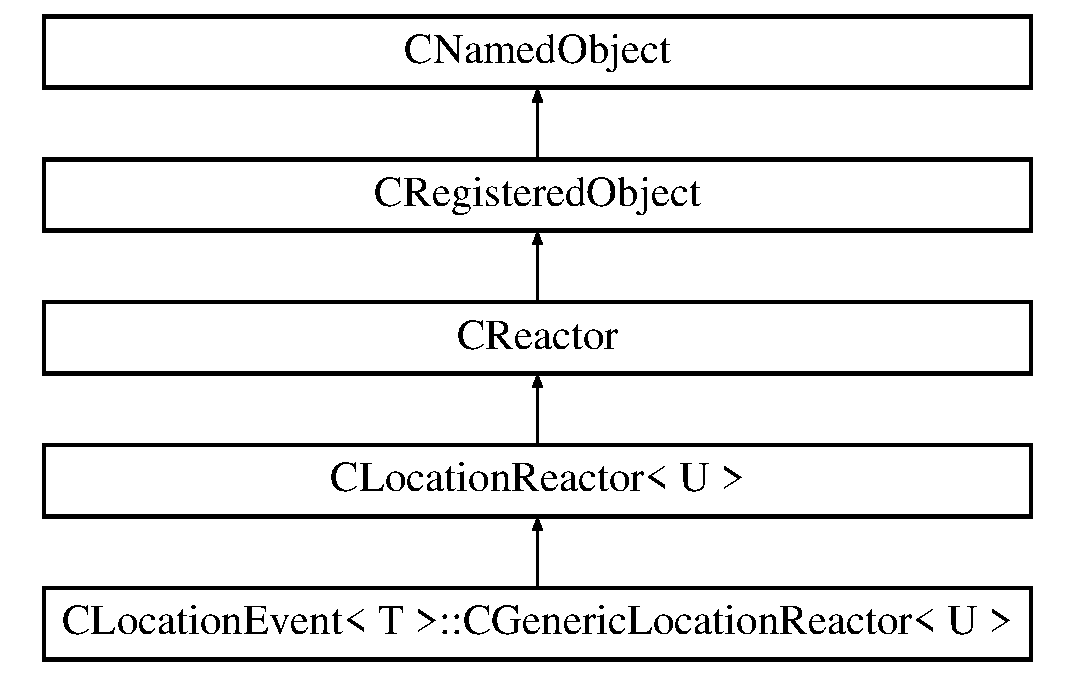
\includegraphics[height=5cm]{classCLocationEvent_1_1CGenericLocationReactor}
\end{center}
\end{figure}
\subsection*{Public Methods}
\begin{CompactItemize}
\item 
{\bf CGeneric\-Location\-Reactor} ({\bf CLocation\-Event}$<$ T $>$ \&r\-Owner)
\item 
virtual void {\bf On\-Location\-Changed} ({\bf CLocation\-Monitor}$<$ T $>$ \&r\-Event, T New\-Value)
\item 
virtual void {\bf On\-Timeout} ({\bf CEvent\-Monitor} \&r\-Event)
\end{CompactItemize}
\subsection*{Private Attributes}
\begin{CompactItemize}
\item 
{\bf CLocation\-Event}$<$ T $>$ \& {\bf m\_\-r\-Owner}
\end{CompactItemize}


\subsection{Detailed Description}
\subsubsection*{template$<$class T$>$template$<$class U$>$ class CLocation\-Event$<$ T $>$::CGeneric\-Location\-Reactor$<$ U $>$}

Nested class CLocation\-Event::CLocation\-Reactor This class is used to give events a monolithic appearance. They relay calls to the Reactor action member functions to corresponding event members. This allows the user of this class to create response by simply subclassing this class rather than forcing them to be aware of the relationship between monitors and reactors. 



Definition at line 348 of file CLocation\-Event.h.

\subsection{Constructor \& Destructor Documentation}
\index{CLocationEvent::CGenericLocationReactor@{CLocation\-Event::CGeneric\-Location\-Reactor}!CGenericLocationReactor@{CGenericLocationReactor}}
\index{CGenericLocationReactor@{CGenericLocationReactor}!CLocationEvent::CGenericLocationReactor@{CLocation\-Event::CGeneric\-Location\-Reactor}}
\subsubsection{\setlength{\rightskip}{0pt plus 5cm}template$<$class T$>$ template$<$class U$>$ {\bf CLocation\-Event}$<$ T $>$::CGeneric\-Location\-Reactor$<$ U $>$::CGeneric\-Location\-Reactor ({\bf CLocation\-Event}$<$ T $>$ \& {\em r\-Owner})}\label{classCLocationEvent_1_1CGenericLocationReactor_a0}


Constructor. Builds a location reactor for {\bf CLocation\-Event} {\rm (p.\,\pageref{classCLocationEvent})} objects. We just keep track of our 'owner' so we know how to callback.\begin{Desc}
\item[Parameters: ]\par
\begin{description}
\item[{\em 
r\-Owner}]- Reference to our owner object. \end{description}
\end{Desc}


Definition at line 308 of file CLocation\-Event.cpp.

\subsection{Member Function Documentation}
\index{CLocationEvent::CGenericLocationReactor@{CLocation\-Event::CGeneric\-Location\-Reactor}!OnLocationChanged@{OnLocationChanged}}
\index{OnLocationChanged@{OnLocationChanged}!CLocationEvent::CGenericLocationReactor@{CLocation\-Event::CGeneric\-Location\-Reactor}}
\subsubsection{\setlength{\rightskip}{0pt plus 5cm}template$<$class T$>$ template$<$class U$>$ void {\bf CLocation\-Event}$<$ T $>$::CGeneric\-Location\-Reactor$<$ U $>$::On\-Location\-Changed ({\bf CLocation\-Monitor}$<$ T $>$ \& {\em r\-Event}, T {\em New\-Value})\hspace{0.3cm}{\tt  [virtual]}}\label{classCLocationEvent_1_1CGenericLocationReactor_a1}


Called when the location has changed in a manner which is significant to the predicate attached to the event. We delegate the action to the Event object which owns us presenting a monolithic appearance of events to the experimenter.\begin{Desc}
\item[Parameters: ]\par
\begin{description}
\item[{\em 
r\-Event}]- Event which fired the operation. \item[{\em 
New\-Value}]- New value in the location. \end{description}
\end{Desc}


Definition at line 326 of file CLocation\-Event.cpp.

References CLocation\-Event$<$ T $>$::CGeneric\-Location\-Reactor$<$ U $>$::m\_\-r\-Owner.\index{CLocationEvent::CGenericLocationReactor@{CLocation\-Event::CGeneric\-Location\-Reactor}!OnTimeout@{OnTimeout}}
\index{OnTimeout@{OnTimeout}!CLocationEvent::CGenericLocationReactor@{CLocation\-Event::CGeneric\-Location\-Reactor}}
\subsubsection{\setlength{\rightskip}{0pt plus 5cm}template$<$class T$>$ template$<$class U$>$ void {\bf CLocation\-Event}$<$ T $>$::CGeneric\-Location\-Reactor$<$ U $>$::On\-Timeout ({\bf CEvent\-Monitor} \& {\em r\-Event})\hspace{0.3cm}{\tt  [virtual]}}\label{classCLocationEvent_1_1CGenericLocationReactor_a2}


Called when timeout receipt is enabled, and a wait times out.  This function delegates action tot he event object which owns us, presenting a monolithic appearance of events to the experimentalist.\begin{Desc}
\item[Parameters: ]\par
\begin{description}
\item[{\em 
r\-Event}]- Reference to the monitor which timed out. (unused). \end{description}
\end{Desc}


Reimplemented from {\bf CReactor} {\rm (p.\,\pageref{classCReactor_a8})}.

Definition at line 342 of file CLocation\-Event.cpp.

References CLocation\-Event$<$ T $>$::CGeneric\-Location\-Reactor$<$ U $>$::m\_\-r\-Owner.

\subsection{Member Data Documentation}
\index{CLocationEvent::CGenericLocationReactor@{CLocation\-Event::CGeneric\-Location\-Reactor}!m_rOwner@{m\_\-rOwner}}
\index{m_rOwner@{m\_\-rOwner}!CLocationEvent::CGenericLocationReactor@{CLocation\-Event::CGeneric\-Location\-Reactor}}
\subsubsection{\setlength{\rightskip}{0pt plus 5cm}template$<$class T$>$ template$<$class U$>$ {\bf CLocation\-Event}$<$T$>$\& {\bf CLocation\-Event}$<$ T $>$::CGeneric\-Location\-Reactor$<$ U $>$::m\_\-r\-Owner\hspace{0.3cm}{\tt  [private]}}\label{classCLocationEvent_1_1CGenericLocationReactor_o0}




Definition at line 351 of file CLocation\-Event.h.

Referenced by CLocation\-Event$<$ T $>$::CGeneric\-Location\-Reactor$<$ U $>$::On\-Location\-Changed(), and CLocation\-Event$<$ T $>$::CGeneric\-Location\-Reactor$<$ U $>$::On\-Timeout().

The documentation for this class was generated from the following files:\begin{CompactItemize}
\item 
{\bf CLocation\-Event.h}\item 
{\bf CLocation\-Event.cpp}\end{CompactItemize}

\section{CLocation\-Monitor$<$ T $>$  Class Template Reference}
\label{classCLocationMonitor}\index{CLocationMonitor@{CLocation\-Monitor}}
{\tt \#include $<$CLocation\-Monitor.h$>$}

Inheritance diagram for CLocation\-Monitor$<$ T $>$::\begin{figure}[H]
\begin{center}
\leavevmode
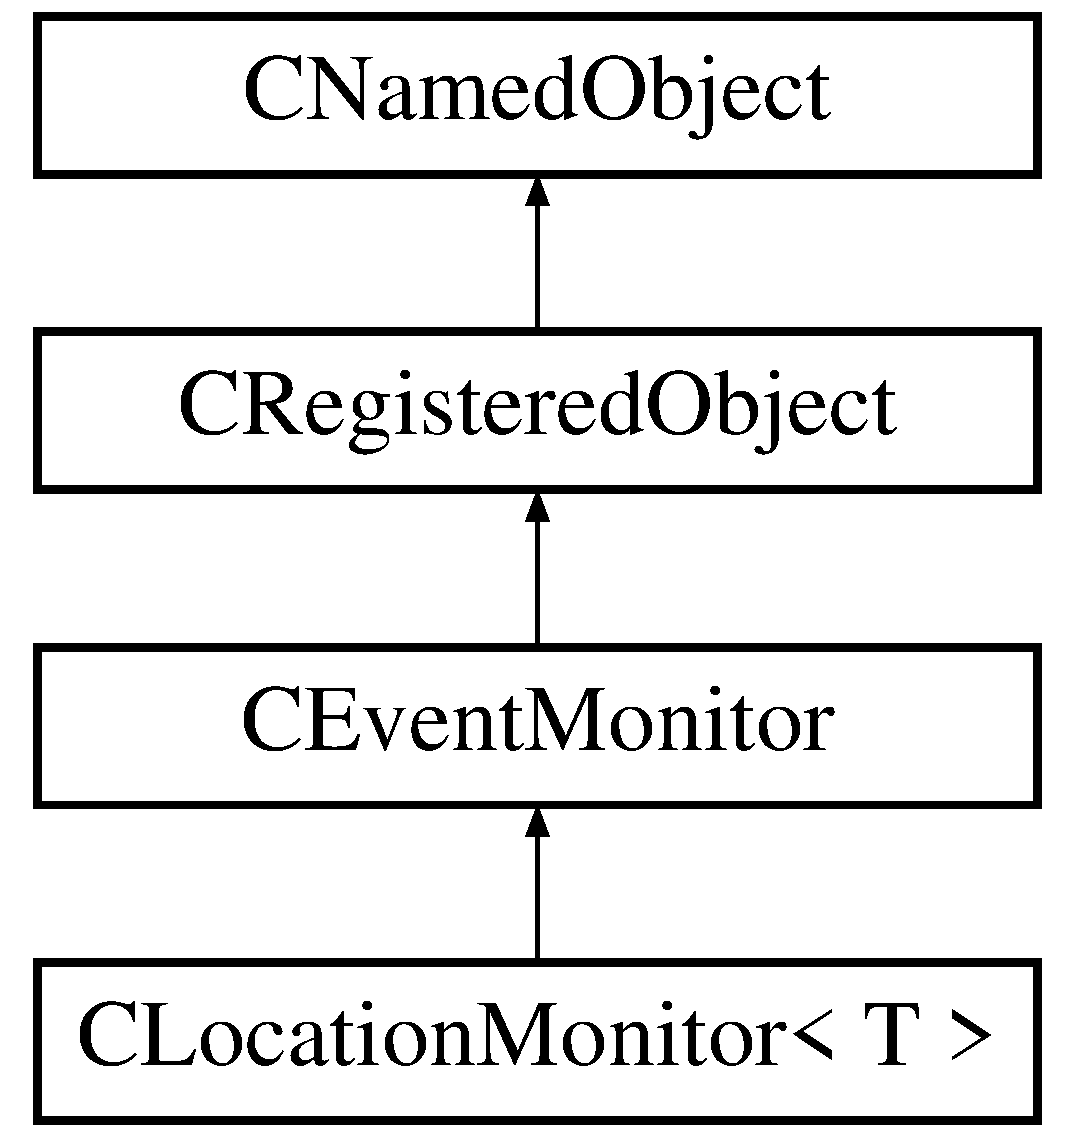
\includegraphics[height=4cm]{classCLocationMonitor}
\end{center}
\end{figure}
\subsection*{Public Methods}
\begin{CompactItemize}
\item 
{\bf CLocation\-Monitor} (volatile T $\ast$am\_\-p\-TLocation, {\bf CPointer\-Predicate}$<$ T $>$ $\ast$am\_\-Predicate, bool am\_\-f\-Timed\-Wait=true)
\item 
{\bf CLocation\-Monitor} (const string \&r\-Name, volatile T $\ast$am\_\-p\-TLocation, {\bf CPointer\-Predicate}$<$ T $>$ $\ast$am\_\-Predicate, bool am\_\-f\-Timed\-Wait=true)
\item 
{\bf CLocation\-Monitor} (const char $\ast$p\-Name, volatile T $\ast$am\_\-p\-TLocation, {\bf CPointer\-Predicate}$<$ T $>$ $\ast$am\_\-Predicate, bool am\_\-f\-Timed\-Wait=true)
\item 
{\bf $\sim$CLocation\-Monitor} ()
\item 
int {\bf operator==} (const CLocation\-Monitor$<$ T $>$ \&a\-CLocation\-Monitor) const
\item 
volatile T $\ast$ {\bf get\-Location} () const
\item 
{\bf CPointer\-Predicate}$<$ T $>$ {\bf get\-Predicate} () const
\item 
virtual {\bf CEvent\-Monitor::result} {\bf operator()} ()
\item 
void {\bf Change\-Location} (T $\ast$p\-New\-Location)
\item 
void {\bf Change\-Predicate} ({\bf CPointer\-Predicate}$<$ T $>$ $\ast$newloc)
\item 
T {\bf get\-Contents} () const
\item 
virtual string {\bf Describe\-Self} ()
\end{CompactItemize}
\subsection*{Protected Methods}
\begin{CompactItemize}
\item 
void {\bf set\-Location} (volatile T $\ast$am\_\-p\-TLocation)
\item 
void {\bf set\-Predicate} ({\bf CPointer\-Predicate}$<$ T $>$ \&am\_\-Predicate)
\end{CompactItemize}
\subsection*{Private Methods}
\begin{CompactItemize}
\item 
{\bf CLocation\-Monitor} (const CLocation\-Monitor$<$ T $>$ \&a\-CLocation\-Monitor)
\item 
CLocation\-Monitor$<$ T $>$ {\bf operator=} (const CLocation\-Monitor$<$ T $>$ \&a\-CLocation\-Monitor)
\end{CompactItemize}
\subsection*{Private Attributes}
\begin{CompactItemize}
\item 
volatile T $\ast$ {\bf m\_\-p\-TLocation}
\item 
{\bf CPointer\-Predicate}$<$ T $>$ $\ast$ {\bf m\_\-Predicate}
\end{CompactItemize}


\subsection{Detailed Description}
\subsubsection*{template$<$typename T$>$ class CLocation\-Monitor$<$ T $>$}

Encapsulates a location monitor.  The location monitor watches a volatile memory location  to satisfy some predicate function object. Predicates are objects from classes which implement: bool operator()(T value) T is a templated variable of the class. Such objects are function objects. The  Event is fired when the predicate returns TRUE. 



Definition at line 335 of file CLocation\-Monitor.h.

\subsection{Constructor \& Destructor Documentation}
\index{CLocationMonitor@{CLocation\-Monitor}!CLocationMonitor@{CLocationMonitor}}
\index{CLocationMonitor@{CLocationMonitor}!CLocationMonitor@{CLocation\-Monitor}}
\subsubsection{\setlength{\rightskip}{0pt plus 5cm}template$<$typename T$>$ CLocation\-Monitor$<$ T $>$::CLocation\-Monitor (volatile T $\ast$ {\em am\_\-p\-TLocation}, {\bf CPointer\-Predicate}$<$ T $>$ $\ast$ {\em am\_\-Predicate}, bool {\em am\_\-f\-Timed\-Wait} = true)\hspace{0.3cm}{\tt  [inline]}}\label{classCLocationMonitor_a0}


associated predicate \index{CLocationMonitor@{CLocation\-Monitor}!CLocationMonitor@{CLocationMonitor}}
\index{CLocationMonitor@{CLocationMonitor}!CLocationMonitor@{CLocation\-Monitor}}
\subsubsection{\setlength{\rightskip}{0pt plus 5cm}template$<$typename T$>$ CLocation\-Monitor$<$ T $>$::CLocation\-Monitor (const string \& {\em r\-Name}, volatile T $\ast$ {\em am\_\-p\-TLocation}, {\bf CPointer\-Predicate}$<$ T $>$ $\ast$ {\em am\_\-Predicate}, bool {\em am\_\-f\-Timed\-Wait} = true)\hspace{0.3cm}{\tt  [inline]}}\label{classCLocationMonitor_a1}


\index{CLocationMonitor@{CLocation\-Monitor}!CLocationMonitor@{CLocationMonitor}}
\index{CLocationMonitor@{CLocationMonitor}!CLocationMonitor@{CLocation\-Monitor}}
\subsubsection{\setlength{\rightskip}{0pt plus 5cm}template$<$typename T$>$ CLocation\-Monitor$<$ T $>$::CLocation\-Monitor (const char $\ast$ {\em p\-Name}, volatile T $\ast$ {\em am\_\-p\-TLocation}, {\bf CPointer\-Predicate}$<$ T $>$ $\ast$ {\em am\_\-Predicate}, bool {\em am\_\-f\-Timed\-Wait} = true)\hspace{0.3cm}{\tt  [inline]}}\label{classCLocationMonitor_a2}


\index{CLocationMonitor@{CLocation\-Monitor}!~CLocationMonitor@{$\sim$CLocationMonitor}}
\index{~CLocationMonitor@{$\sim$CLocationMonitor}!CLocationMonitor@{CLocation\-Monitor}}
\subsubsection{\setlength{\rightskip}{0pt plus 5cm}template$<$typename T$>$ CLocation\-Monitor$<$ T $>$::$\sim$CLocation\-Monitor ()\hspace{0.3cm}{\tt  [inline]}}\label{classCLocationMonitor_a3}


\index{CLocationMonitor@{CLocation\-Monitor}!CLocationMonitor@{CLocationMonitor}}
\index{CLocationMonitor@{CLocationMonitor}!CLocationMonitor@{CLocation\-Monitor}}
\subsubsection{\setlength{\rightskip}{0pt plus 5cm}template$<$typename T$>$ CLocation\-Monitor$<$ T $>$::CLocation\-Monitor (const CLocation\-Monitor$<$ T $>$ \& {\em a\-CLocation\-Monitor})\hspace{0.3cm}{\tt  [private]}}\label{classCLocationMonitor_c0}




\subsection{Member Function Documentation}
\index{CLocationMonitor@{CLocation\-Monitor}!ChangeLocation@{ChangeLocation}}
\index{ChangeLocation@{ChangeLocation}!CLocationMonitor@{CLocation\-Monitor}}
\subsubsection{\setlength{\rightskip}{0pt plus 5cm}template$<$typename T$>$ void CLocation\-Monitor$<$ T $>$::Change\-Location (T $\ast$ {\em p\-New\-Location})}\label{classCLocationMonitor_a8}


Operation Type: Mutator

Purpose: Changes the location monitored. 

Definition at line 354 of file CLocation\-Monitor.cpp.

References CLocation\-Monitor$<$ T $>$::m\_\-p\-TLocation.\index{CLocationMonitor@{CLocation\-Monitor}!ChangePredicate@{ChangePredicate}}
\index{ChangePredicate@{ChangePredicate}!CLocationMonitor@{CLocation\-Monitor}}
\subsubsection{\setlength{\rightskip}{0pt plus 5cm}template$<$typename T$>$ void CLocation\-Monitor$<$ T $>$::Change\-Predicate ({\bf CPointer\-Predicate}$<$ T $>$ $\ast$ {\em new\-Loc})}\label{classCLocationMonitor_a9}


Operation Type: Mutator

Purpose: Associates a new predicate with the  location monitor. 

Definition at line 371 of file CLocation\-Monitor.cpp.

References CLocation\-Monitor$<$ T $>$::m\_\-Predicate.\index{CLocationMonitor@{CLocation\-Monitor}!DescribeSelf@{DescribeSelf}}
\index{DescribeSelf@{DescribeSelf}!CLocationMonitor@{CLocation\-Monitor}}
\subsubsection{\setlength{\rightskip}{0pt plus 5cm}template$<$typename T$>$ string CLocation\-Monitor$<$ T $>$::Describe\-Self ()\hspace{0.3cm}{\tt  [virtual]}}\label{classCLocationMonitor_a11}


Operation Type: Selector

Purpose: Returns a string which describes the monitor. Inlcudes: 1. {\bf CEvent\-Monitor::Describe\-Self} {\rm (p.\,\pageref{classCNamedObject_a8})} 2. Dumps of the pointer value, 3. m\_\-Predicate-$>${\bf Describe\-Self}() {\rm (p.\,\pageref{classCLocationMonitor_a11})} 

Reimplemented from {\bf CNamed\-Object} {\rm (p.\,\pageref{classCNamedObject_a8})}.

Definition at line 390 of file CLocation\-Monitor.cpp.

References CNamed\-Object::Describe\-Self(), CLocation\-Monitor$<$ T $>$::m\_\-Predicate, and CLocation\-Monitor$<$ T $>$::m\_\-p\-TLocation.\index{CLocationMonitor@{CLocation\-Monitor}!getContents@{getContents}}
\index{getContents@{getContents}!CLocationMonitor@{CLocation\-Monitor}}
\subsubsection{\setlength{\rightskip}{0pt plus 5cm}template$<$typename T$>$ T CLocation\-Monitor$<$ T $>$::get\-Contents () const\hspace{0.3cm}{\tt  [inline]}}\label{classCLocationMonitor_a10}




Definition at line 419 of file CLocation\-Monitor.h.\index{CLocationMonitor@{CLocation\-Monitor}!getLocation@{getLocation}}
\index{getLocation@{getLocation}!CLocationMonitor@{CLocation\-Monitor}}
\subsubsection{\setlength{\rightskip}{0pt plus 5cm}template$<$typename T$>$ volatile T$\ast$ CLocation\-Monitor$<$ T $>$::get\-Location () const\hspace{0.3cm}{\tt  [inline]}}\label{classCLocationMonitor_a5}




Definition at line 390 of file CLocation\-Monitor.h.

References CLocation\-Monitor$<$ T $>$::m\_\-p\-TLocation.

Referenced by CLocation\-Event$<$ T $>$::get\-Pointer(), and CLocation\-Reactor$<$ T $>$::On\-Event().\index{CLocationMonitor@{CLocation\-Monitor}!getPredicate@{getPredicate}}
\index{getPredicate@{getPredicate}!CLocationMonitor@{CLocation\-Monitor}}
\subsubsection{\setlength{\rightskip}{0pt plus 5cm}template$<$typename T$>$ {\bf CPointer\-Predicate}$<$T$>$ CLocation\-Monitor$<$ T $>$::get\-Predicate () const\hspace{0.3cm}{\tt  [inline]}}\label{classCLocationMonitor_a6}




Definition at line 395 of file CLocation\-Monitor.h.\index{CLocationMonitor@{CLocation\-Monitor}!operator()@{operator()}}
\index{operator()@{operator()}!CLocationMonitor@{CLocation\-Monitor}}
\subsubsection{\setlength{\rightskip}{0pt plus 5cm}template$<$typename T$>$ {\bf CEvent\-Monitor::result} CLocation\-Monitor$<$ T $>$::operator() ()\hspace{0.3cm}{\tt  [virtual]}}\label{classCLocationMonitor_a7}


Operation Type: Override behavior

Purpose: Reads the current value of the location and passes it to the predicate. Returns: 1. Occured - if the predicate returned TRUE 2. Timed\-Out - if the wait time for this event timedout. 3. Error - If the predicate threw an exception. 

Implements {\bf CEvent\-Monitor} {\rm (p.\,\pageref{classCEventMonitor_a7})}.

Definition at line 315 of file CLocation\-Monitor.cpp.

References CEvent\-Monitor::Error, CEvent\-Monitor::get\-Timeout(), INCREMENTS, CLocation\-Monitor$<$ T $>$::m\_\-Predicate, CEvent\-Monitor::Occurred, and CEvent\-Monitor::Timed\-Out.\index{CLocationMonitor@{CLocation\-Monitor}!operator=@{operator=}}
\index{operator=@{operator=}!CLocationMonitor@{CLocation\-Monitor}}
\subsubsection{\setlength{\rightskip}{0pt plus 5cm}template$<$typename T$>$ CLocation\-Monitor$<$T$>$ CLocation\-Monitor$<$ T $>$::operator= (const CLocation\-Monitor$<$ T $>$ \& {\em a\-CLocation\-Monitor})\hspace{0.3cm}{\tt  [private]}}\label{classCLocationMonitor_c1}


\index{CLocationMonitor@{CLocation\-Monitor}!operator==@{operator==}}
\index{operator==@{operator==}!CLocationMonitor@{CLocation\-Monitor}}
\subsubsection{\setlength{\rightskip}{0pt plus 5cm}template$<$typename T$>$ int CLocation\-Monitor$<$ T $>$::operator== (const CLocation\-Monitor$<$ T $>$ \& {\em a\-CLocation\-Monitor}) const\hspace{0.3cm}{\tt  [inline]}}\label{classCLocationMonitor_a4}




Definition at line 371 of file CLocation\-Monitor.h.

References CLocation\-Monitor$<$ T $>$::m\_\-Predicate, CLocation\-Monitor$<$ T $>$::m\_\-p\-TLocation, and CEvent\-Monitor::operator==().\index{CLocationMonitor@{CLocation\-Monitor}!setLocation@{setLocation}}
\index{setLocation@{setLocation}!CLocationMonitor@{CLocation\-Monitor}}
\subsubsection{\setlength{\rightskip}{0pt plus 5cm}template$<$typename T$>$ void CLocation\-Monitor$<$ T $>$::set\-Location (volatile T $\ast$ {\em am\_\-p\-TLocation})\hspace{0.3cm}{\tt  [inline, protected]}}\label{classCLocationMonitor_b0}




Definition at line 403 of file CLocation\-Monitor.h.

References CLocation\-Monitor$<$ T $>$::m\_\-p\-TLocation.\index{CLocationMonitor@{CLocation\-Monitor}!setPredicate@{setPredicate}}
\index{setPredicate@{setPredicate}!CLocationMonitor@{CLocation\-Monitor}}
\subsubsection{\setlength{\rightskip}{0pt plus 5cm}template$<$typename T$>$ void CLocation\-Monitor$<$ T $>$::set\-Predicate ({\bf CPointer\-Predicate}$<$ T $>$ \& {\em am\_\-Predicate})\hspace{0.3cm}{\tt  [inline, protected]}}\label{classCLocationMonitor_b1}




Definition at line 408 of file CLocation\-Monitor.h.

\subsection{Member Data Documentation}
\index{CLocationMonitor@{CLocation\-Monitor}!m_Predicate@{m\_\-Predicate}}
\index{m_Predicate@{m\_\-Predicate}!CLocationMonitor@{CLocation\-Monitor}}
\subsubsection{\setlength{\rightskip}{0pt plus 5cm}template$<$typename T$>$ {\bf CPointer\-Predicate}$<$T$>$$\ast$ CLocation\-Monitor$<$ T $>$::m\_\-Predicate\hspace{0.3cm}{\tt  [private]}}\label{classCLocationMonitor_o1}


Location monitored 

Definition at line 338 of file CLocation\-Monitor.h.

Referenced by CLocation\-Monitor$<$ T $>$::Change\-Predicate(), CLocation\-Monitor$<$ T $>$::Describe\-Self(), CLocation\-Monitor$<$ T $>$::operator()(), and CLocation\-Monitor$<$ T $>$::operator==().\index{CLocationMonitor@{CLocation\-Monitor}!m_pTLocation@{m\_\-pTLocation}}
\index{m_pTLocation@{m\_\-pTLocation}!CLocationMonitor@{CLocation\-Monitor}}
\subsubsection{\setlength{\rightskip}{0pt plus 5cm}template$<$typename T$>$ volatile T$\ast$ CLocation\-Monitor$<$ T $>$::m\_\-p\-TLocation\hspace{0.3cm}{\tt  [private]}}\label{classCLocationMonitor_o0}




Definition at line 337 of file CLocation\-Monitor.h.

Referenced by CLocation\-Monitor$<$ T $>$::Change\-Location(), CLocation\-Monitor$<$ T $>$::Describe\-Self(), CLocation\-Monitor$<$ T $>$::get\-Location(), CLocation\-Monitor$<$ T $>$::operator==(), and CLocation\-Monitor$<$ T $>$::set\-Location().

The documentation for this class was generated from the following files:\begin{CompactItemize}
\item 
{\bf CLocation\-Monitor.h}\item 
{\bf CLocation\-Monitor.cpp}\end{CompactItemize}

\section{CLocation\-Reactor$<$ T $>$  Class Template Reference}
\label{classCLocationReactor}\index{CLocationReactor@{CLocation\-Reactor}}
{\tt \#include $<$CLocation\-Reactor.h$>$}

Inheritance diagram for CLocation\-Reactor$<$ T $>$::\begin{figure}[H]
\begin{center}
\leavevmode
\includegraphics[height=4cm]{classCLocationReactor}
\end{center}
\end{figure}
\subsection*{Public Methods}
\begin{CompactItemize}
\item 
{\bf CLocation\-Reactor} ()
\item 
{\bf CLocation\-Reactor} (const string \&r\-Name)
\item 
{\bf CLocation\-Reactor} (const char $\ast$p\-Name)
\item 
{\bf $\sim$CLocation\-Reactor} ()
\begin{CompactList}\small\item\em Destructor:.\item\end{CompactList}\item 
template$<$class U$>$ int {\bf operator==} (const CLocation\-Reactor$<$ U $>$ \&a\-CLocation\-Reactor) const
\begin{CompactList}\small\item\em Operator== Equality Operator is allowed, but doesn't mean much.\item\end{CompactList}\item 
virtual void {\bf On\-Event} ({\bf CEvent\-Monitor} \&r\-Event)
\item 
virtual void {\bf On\-Location\-Changed} ({\bf CLocation\-Monitor}$<$ T $>$ \&r\-Event, T new\-Value)
\end{CompactItemize}
\subsection*{Private Methods}
\begin{CompactItemize}
\item 
{\bf CLocation\-Reactor} (const CLocation\-Reactor \&a\-CLocation\-Reactor)
\begin{CompactList}\small\item\em Copy Constructor is not allowed.\item\end{CompactList}\item 
CLocation\-Reactor \& {\bf operator=} (const CLocation\-Reactor \&a\-CLocation\-Reactor)
\begin{CompactList}\small\item\em Operator= Assignment Operator is not allowed.\item\end{CompactList}\end{CompactItemize}


\subsection{Detailed Description}
\subsubsection*{template$<$class T$>$ class CLocation\-Reactor$<$ T $>$}

Reacts to location monitor events. A location monitor monitors a Specific volatile object for various abstract conditions checked by a predicate. This is an abstract base class which must be derived for a particular applciation. The purpose of this class is to provide a branch in the Reactor class hierarchy from which Location Monitors can determine comptibility of the reactor. This class should be templated by the type used to template the monitor. 



Definition at line 318 of file CLocation\-Reactor.h.

\subsection{Constructor \& Destructor Documentation}
\index{CLocationReactor@{CLocation\-Reactor}!CLocationReactor@{CLocationReactor}}
\index{CLocationReactor@{CLocationReactor}!CLocationReactor@{CLocation\-Reactor}}
\subsubsection{\setlength{\rightskip}{0pt plus 5cm}template$<$class T$>$ CLocation\-Reactor$<$ T $>$::CLocation\-Reactor ()}\label{classCLocationReactor_a0}


Default Constructor: Creates a reactor with an autoassigned name. There's currently no way to know by looking at the name that this is a Location Reactor 

Definition at line 315 of file CLocation\-Reactor.cpp.

References CNamed\-Object::Append\-Class\-Info().\index{CLocationReactor@{CLocation\-Reactor}!CLocationReactor@{CLocationReactor}}
\index{CLocationReactor@{CLocationReactor}!CLocationReactor@{CLocation\-Reactor}}
\subsubsection{\setlength{\rightskip}{0pt plus 5cm}template$<$class T$>$ CLocation\-Reactor$<$ T $>$::CLocation\-Reactor (const string \& {\em r\-Name})}\label{classCLocationReactor_a1}


Constructor given a name in STL String form. \begin{Desc}
\item[Parameters: ]\par
\begin{description}
\item[{\em 
r\-Name}]- name of the object. \end{description}
\end{Desc}


Definition at line 326 of file CLocation\-Reactor.cpp.

References CNamed\-Object::Append\-Class\-Info().\index{CLocationReactor@{CLocation\-Reactor}!CLocationReactor@{CLocationReactor}}
\index{CLocationReactor@{CLocationReactor}!CLocationReactor@{CLocation\-Reactor}}
\subsubsection{\setlength{\rightskip}{0pt plus 5cm}template$<$class T$>$ CLocation\-Reactor$<$ T $>$::CLocation\-Reactor (const char $\ast$ {\em p\-Name})}\label{classCLocationReactor_a2}


Constructor given a name in ASCIZ format. \begin{Desc}
\item[Parameters: ]\par
\begin{description}
\item[{\em 
p\-Name}]- pointer to the ASCIZ name of the object to create. \end{description}
\end{Desc}


Definition at line 336 of file CLocation\-Reactor.cpp.

References CNamed\-Object::Append\-Class\-Info().\index{CLocationReactor@{CLocation\-Reactor}!~CLocationReactor@{$\sim$CLocationReactor}}
\index{~CLocationReactor@{$\sim$CLocationReactor}!CLocationReactor@{CLocation\-Reactor}}
\subsubsection{\setlength{\rightskip}{0pt plus 5cm}template$<$class T$>$ CLocation\-Reactor$<$ T $>$::$\sim$CLocation\-Reactor ()}\label{classCLocationReactor_a3}


Destructor:.



Definition at line 343 of file CLocation\-Reactor.cpp.\index{CLocationReactor@{CLocation\-Reactor}!CLocationReactor@{CLocationReactor}}
\index{CLocationReactor@{CLocationReactor}!CLocationReactor@{CLocation\-Reactor}}
\subsubsection{\setlength{\rightskip}{0pt plus 5cm}template$<$class T$>$ CLocation\-Reactor$<$ T $>$::CLocation\-Reactor (const CLocation\-Reactor$<$ T $>$ \& {\em a\-CLocation\-Reactor})\hspace{0.3cm}{\tt  [private]}}\label{classCLocationReactor_c0}


Copy Constructor is not allowed.



\subsection{Member Function Documentation}
\index{CLocationReactor@{CLocation\-Reactor}!OnEvent@{OnEvent}}
\index{OnEvent@{OnEvent}!CLocationReactor@{CLocation\-Reactor}}
\subsubsection{\setlength{\rightskip}{0pt plus 5cm}template$<$class T$>$ void CLocation\-Reactor$<$ T $>$::On\-Event ({\bf CEvent\-Monitor} \& {\em r\-Event})\hspace{0.3cm}{\tt  [virtual]}}\label{classCLocationReactor_a5}


Called when an event occurs.  The base class is overriddent to dynamically cast the  r\-Event parameter to a {\bf CLocation\-Monitor} {\rm (p.\,\pageref{classCLocationMonitor})}$<$T$>$ reference, and then get the value pointed to by the pointer. Once this is done, On\-Location\-Changed is called. THus users of this class typically will only need to derive and override On\-Location\-Changed.\begin{Desc}
\item[Parameters: ]\par
\begin{description}
\item[{\em 
r\-Event}]- Reference to the {\bf CEvent\-Monitor} {\rm (p.\,\pageref{classCEventMonitor})} which was monitoring us. \end{description}
\end{Desc}


Reimplemented from {\bf CReactor} {\rm (p.\,\pageref{classCReactor_a6})}.

Definition at line 371 of file CLocation\-Reactor.cpp.

References CLocation\-Monitor$<$ T $>$::get\-Location(), and CLocation\-Reactor$<$ T $>$::On\-Location\-Changed().\index{CLocationReactor@{CLocation\-Reactor}!OnLocationChanged@{OnLocationChanged}}
\index{OnLocationChanged@{OnLocationChanged}!CLocationReactor@{CLocation\-Reactor}}
\subsubsection{\setlength{\rightskip}{0pt plus 5cm}template$<$class T$>$ void CLocation\-Reactor$<$ T $>$::On\-Location\-Changed ({\bf CLocation\-Monitor}$<$ T $>$ \& {\em r\-Event}, T {\em new\-Value})\hspace{0.3cm}{\tt  [virtual]}}\label{classCLocationReactor_a6}


Called when a location monitor detects a location change which satisfies its predicate. I expect that this Reactor will be used minimally by subclassing this class and overriding this function with application specific code.\begin{Desc}
\item[Parameters: ]\par
\begin{description}
\item[{\em 
r\-Event}]- Reference to the location monitor which fired us. \item[{\em 
new\-Value}]- New value at the location being monitored. \end{description}
\end{Desc}


Definition at line 402 of file CLocation\-Reactor.cpp.

Referenced by CLocation\-Reactor$<$ T $>$::On\-Event().\index{CLocationReactor@{CLocation\-Reactor}!operator=@{operator=}}
\index{operator=@{operator=}!CLocationReactor@{CLocation\-Reactor}}
\subsubsection{\setlength{\rightskip}{0pt plus 5cm}template$<$class T$>$ CLocation\-Reactor\& CLocation\-Reactor$<$ T $>$::operator= (const CLocation\-Reactor$<$ T $>$ \& {\em a\-CLocation\-Reactor})\hspace{0.3cm}{\tt  [private]}}\label{classCLocationReactor_c1}


Operator= Assignment Operator is not allowed.

\index{CLocationReactor@{CLocation\-Reactor}!operator==@{operator==}}
\index{operator==@{operator==}!CLocationReactor@{CLocation\-Reactor}}
\subsubsection{\setlength{\rightskip}{0pt plus 5cm}template$<$class T$>$ template$<$class U$>$ int CLocation\-Reactor$<$ T $>$::operator== (const CLocation\-Reactor$<$ U $>$ \& {\em a\-CLocation\-Reactor}) const}\label{classCLocationReactor_a4}


Operator== Equality Operator is allowed, but doesn't mean much.



Definition at line 351 of file CLocation\-Reactor.cpp.

References CReactor::operator==().

The documentation for this class was generated from the following files:\begin{CompactItemize}
\item 
{\bf CLocation\-Reactor.h}\item 
{\bf CLocation\-Reactor.cpp}\end{CompactItemize}

\section{CLogger  Class Reference}
\label{classCLogger}\index{CLogger@{CLogger}}
{\tt \#include $<$CLogger.h$>$}

\subsection*{Public Types}
\begin{CompactItemize}
\item 
enum {\bf Severity} \{ {\bf SUCCESS}, 
{\bf WARNING}, 
{\bf ERROR}
 \}
\begin{CompactList}\small\item\em The facility name which is logging the event.\item\end{CompactList}\end{CompactItemize}
\subsection*{Public Methods}
\begin{CompactItemize}
\item 
{\bf CLogger} (string facility)
\item 
{\bf CLogger} (const CLogger \&a\-CLogger)
\item 
{\bf $\sim$CLogger} ()
\item 
bool {\bf Log} ({\bf Severity} sev, string message)
\item 
{\bf Host\-List\-Iterator} {\bf begin} ()
\item 
{\bf Host\-List\-Iterator} {\bf end} ()
\item 
int {\bf size} ()
\item 
void {\bf Add\-Host} (const string \&new\-Host)
\item 
void {\bf Remove\-Host} (const string \&old\-Host)
\item 
void {\bf Remove\-Host} ({\bf Host\-List\-Iterator} It)
\end{CompactItemize}
\subsection*{Private Methods}
\begin{CompactItemize}
\item 
CLogger {\bf operator=} (const CLogger \&a\-CLogger)
\item 
int {\bf operator==} (const CLogger \&a\-CLogger)
\item 
list$<$ string $>$ {\bf get\-Host\-List} () const
\item 
const string {\bf get\-Facility} () const
\end{CompactItemize}
\subsection*{Private Attributes}
\begin{CompactItemize}
\item 
list$<$ string $>$ {\bf m\_\-Host\-List}
\item 
const string {\bf m\_\-s\-Facility}
\begin{CompactList}\small\item\em The list of hosts running Event\-Log.tcl.\item\end{CompactList}\end{CompactItemize}


\subsection{Detailed Description}
Encapsulates a logger class for events which occur in the data acquisition framework.  The Logger maintains a list of hostnames on which the actual Event\-Log.tcl script is running, as well as the port number and name of the facility which contains it. An event is logged via a call to the {\bf CLogger::Log}() {\rm (p.\,\pageref{classCLogger_a3})} function member which creates  client sockets that connect to each of the hosts in the host list and logs the events. Each socket is shut down immediately  after the log entry is written. CLogger also contains an enumeration {\bf CLogger::Severity} {\rm (p.\,\pageref{classCLogger_s3})}. This is used for function {\bf CLogger::Log}() {\rm (p.\,\pageref{classCLogger_a3})}, as there are only three possible values for severity that the logger will accept:

\begin{CompactItemize}
\item 
SUCCESS: The operation being logged completed successfully.\item 
WARNING: The operation being logged completed, but there was a warning issued by the application.\item 
ERROR: The operation being logged did not complete, and an exceptional condition was encountered. \end{CompactItemize}




Definition at line 347 of file CLogger.h.

\subsection{Member Enumeration Documentation}
\index{CLogger@{CLogger}!Severity@{Severity}}
\index{Severity@{Severity}!CLogger@{CLogger}}
\subsubsection{\setlength{\rightskip}{0pt plus 5cm}enum CLogger::Severity}\label{classCLogger_s3}


The facility name which is logging the event.

\begin{Desc}
\item[Enumeration values:]\par
\begin{description}
\index{SUCCESS@{SUCCESS}!CLogger@{CLogger}}\index{CLogger@{CLogger}!SUCCESS@{SUCCESS}}\item[{\em 
{\em SUCCESS}\label{classCLogger_s3s0}
}]\index{WARNING@{WARNING}!CLogger@{CLogger}}\index{CLogger@{CLogger}!WARNING@{WARNING}}\item[{\em 
{\em WARNING}\label{classCLogger_s3s1}
}]\index{ERROR@{ERROR}!CLogger@{CLogger}}\index{CLogger@{CLogger}!ERROR@{ERROR}}\item[{\em 
{\em ERROR}\label{classCLogger_s3s2}
}]\end{description}
\end{Desc}



Definition at line 353 of file CLogger.h.

\subsection{Constructor \& Destructor Documentation}
\index{CLogger@{CLogger}!CLogger@{CLogger}}
\index{CLogger@{CLogger}!CLogger@{CLogger}}
\subsubsection{\setlength{\rightskip}{0pt plus 5cm}CLogger::CLogger (string {\em facility})}\label{classCLogger_a0}


\char`\"{}Default Constructor\char`\"{} This is the default constructor which constructs a CLogger given a list of hosts to which it will form socket connections when logging events, and a facility name which will be the name of the facility doing the logging.\begin{Desc}
\item[Parameters: ]\par
\begin{description}
\item[{\em 
facility}]- the name of the facility doing the logging \end{description}
\end{Desc}


Definition at line 310 of file CLogger.cpp.\index{CLogger@{CLogger}!CLogger@{CLogger}}
\index{CLogger@{CLogger}!CLogger@{CLogger}}
\subsubsection{\setlength{\rightskip}{0pt plus 5cm}CLogger::CLogger (const CLogger \& {\em a\-CLogger})}\label{classCLogger_a1}


\char`\"{}Copy Constructor\char`\"{} This is the copy constructor. It creates a new object by copying the information of the reference object which is its parameter.\begin{Desc}
\item[Parameters: ]\par
\begin{description}
\item[{\em 
a\-CLogger}]- the reference object whose attributes will be copied. \end{description}
\end{Desc}


Definition at line 320 of file CLogger.cpp.\index{CLogger@{CLogger}!~CLogger@{$\sim$CLogger}}
\index{~CLogger@{$\sim$CLogger}!CLogger@{CLogger}}
\subsubsection{\setlength{\rightskip}{0pt plus 5cm}CLogger::$\sim$CLogger ()}\label{classCLogger_a2}


\char`\"{}Destructor\char`\"{} Called when an object goes out of scope, or when execution of the program is terminated. Destroys the object, and frees up space. 

Definition at line 329 of file CLogger.cpp.

\subsection{Member Function Documentation}
\index{CLogger@{CLogger}!AddHost@{AddHost}}
\index{AddHost@{AddHost}!CLogger@{CLogger}}
\subsubsection{\setlength{\rightskip}{0pt plus 5cm}void CLogger::Add\-Host (const string \& {\em new\-Host})}\label{classCLogger_a7}


Operation Type: Mutator

Purpose: Adds a host to the list of hosts that we will attempt to form a connection with and log a message to.\begin{Desc}
\item[Parameters: ]\par
\begin{description}
\item[{\em 
const}]string\& new\-Host The name of the new host to be  added to m\_\-Host\-List\end{description}
\end{Desc}
\begin{Desc}
\item[Exceptions: ]\par
\begin{description}
\item[{\em 
{\bf CDuplicate\-Name\-Exception} {\rm (p.\,\pageref{classCDuplicateNameException})}}] Thrown if the host already  exists in the host list \end{description}
\end{Desc}


Definition at line 517 of file CLogger.cpp.

References Host\-List\-Iterator, and m\_\-Host\-List.\index{CLogger@{CLogger}!begin@{begin}}
\index{begin@{begin}!CLogger@{CLogger}}
\subsubsection{\setlength{\rightskip}{0pt plus 5cm}{\bf Host\-List\-Iterator} CLogger::begin ()}\label{classCLogger_a4}


Operation Type: Selector

Purpose: Returns an iterator to the first host in m\_\-Host\-List. 

Definition at line 468 of file CLogger.cpp.

References m\_\-Host\-List.\index{CLogger@{CLogger}!end@{end}}
\index{end@{end}!CLogger@{CLogger}}
\subsubsection{\setlength{\rightskip}{0pt plus 5cm}{\bf Host\-List\-Iterator} CLogger::end ()}\label{classCLogger_a5}


Operator Type: Selector

Purpose: Returns an iterator which points to just past the last host in m\_\-Host\-List. 

Definition at line 482 of file CLogger.cpp.

References m\_\-Host\-List.\index{CLogger@{CLogger}!getFacility@{getFacility}}
\index{getFacility@{getFacility}!CLogger@{CLogger}}
\subsubsection{\setlength{\rightskip}{0pt plus 5cm}const string CLogger::get\-Facility () const\hspace{0.3cm}{\tt  [inline, private]}}\label{classCLogger_c3}




Definition at line 377 of file CLogger.h.

References m\_\-s\-Facility.\index{CLogger@{CLogger}!getHostList@{getHostList}}
\index{getHostList@{getHostList}!CLogger@{CLogger}}
\subsubsection{\setlength{\rightskip}{0pt plus 5cm}list$<$string$>$ CLogger::get\-Host\-List () const\hspace{0.3cm}{\tt  [inline, private]}}\label{classCLogger_c2}




Definition at line 376 of file CLogger.h.

References m\_\-Host\-List.\index{CLogger@{CLogger}!Log@{Log}}
\index{Log@{Log}!CLogger@{CLogger}}
\subsubsection{\setlength{\rightskip}{0pt plus 5cm}bool CLogger::Log ({\bf Severity} {\em sev}, string {\em message})}\label{classCLogger_a3}


Operation Type: Log to file and screen

Attempts to log a message (facility, severity, message, date) to  Event\-Log.tcl by opening a socket connection to each of the hosts in m\_\-Host\-List. The first connection logs the message which consists of the facility, severity, and message to the log file via a call to the tcl procedure Logger::Log. This only needs to be written once, since the same log file will be used by each displayer. The Logger::Log tcl procedure obtains the exact time of the event via a call to date(1). It then returns the date string through the socket (which we read) and that string is what is displayed on the GUI via a call to Logger::Display\_\-Event. In this way, the date on each display will be exactly the same. NOTE: If {\bf Log}() {\rm (p.\,\pageref{classCLogger_a3})} fails for the first host in the list, then the event will not be written to the log file and will not be displayed anywhere.  If connection to the first host succeeds, but fails on a subsequent host, the event will be logged to file but will not be displayed on whichever host connection failed. It will, however, be displayed on all hosts (including subsequent hosts) to which connection does not fail.\begin{Desc}
\item[Exceptions: ]\par
\begin{description}
\item[{\em 
{\bf CErrno\-Exception} {\rm (p.\,\pageref{classCErrnoException})}}] - Errno exception occurred \item[{\em 
{\bf CTCPBad\-Socket\-State} {\rm (p.\,\pageref{classCTCPBadSocketState})}}] - {\bf CSocket::m\_\-State} {\rm (p.\,\pageref{classCSocket_o1})} was not disconnected \item[{\em 
{\bf CTCPNo\-Such\-Host} {\rm (p.\,\pageref{classCTCPNoSuchHost})}}] - Host not in DNS or nonexistent \item[{\em 
{\bf CTCPNo\-Such\-Service} {\rm (p.\,\pageref{classCTCPNoSuchService})}}] - Named service does not translate. \item[{\em 
{\bf CTCPConnection\-Failed} {\rm (p.\,\pageref{classCTCPConnectionFailed})}}] - Connection refused by remote host \item[{\em 
{\bf CTCPConnection\-Lost} {\rm (p.\,\pageref{classCTCPConnectionLost})}}] - Connection terminated by remote host\end{description}
\end{Desc}
\begin{Desc}
\item[Parameters: ]\par
\begin{description}
\item[{\em 
sev}]- This is an enumerated value which represent the severity of the event. \item[{\em 
message}]- This is the message which the caller wants to log. \end{description}
\end{Desc}


Definition at line 365 of file CLogger.cpp.

References CSocket::Connect(), ERROR, m\_\-Host\-List, m\_\-s\-Facility, PORT, CSocket::Read(), CSocket::Shutdown(), SUCCESS, WARNING, and CSocket::Write().\index{CLogger@{CLogger}!operator=@{operator=}}
\index{operator=@{operator=}!CLogger@{CLogger}}
\subsubsection{\setlength{\rightskip}{0pt plus 5cm}CLogger CLogger::operator= (const CLogger \& {\em a\-CLogger})\hspace{0.3cm}{\tt  [private]}}\label{classCLogger_c0}


\index{CLogger@{CLogger}!operator==@{operator==}}
\index{operator==@{operator==}!CLogger@{CLogger}}
\subsubsection{\setlength{\rightskip}{0pt plus 5cm}int CLogger::operator== (const CLogger \& {\em a\-CLogger})\hspace{0.3cm}{\tt  [private]}}\label{classCLogger_c1}


\index{CLogger@{CLogger}!RemoveHost@{RemoveHost}}
\index{RemoveHost@{RemoveHost}!CLogger@{CLogger}}
\subsubsection{\setlength{\rightskip}{0pt plus 5cm}void CLogger::Remove\-Host ({\bf Host\-List\-Iterator} {\em It})}\label{classCLogger_a9}


Operation Type: Mutator

Purpose: Removes a host from the list of hosts that we will attempt to form a connection with and log a message to.\begin{Desc}
\item[Parameters: ]\par
\begin{description}
\item[{\em 
Host\-List\-Iterator}]It An iterator which points to the host in m\_\-Host\-List that is to be removed. \end{description}
\end{Desc}
\begin{Desc}
\item[Exceptions: ]\par
\begin{description}
\item[{\em 
{\bf CNo\-Such\-Object\-Exception} {\rm (p.\,\pageref{classCNoSuchObjectException})}}] Thrown if the name supplied in the paramter is not in m\_\-Host\-List. \end{description}
\end{Desc}


Definition at line 574 of file CLogger.cpp.

References Host\-List\-Iterator, and m\_\-Host\-List.\index{CLogger@{CLogger}!RemoveHost@{RemoveHost}}
\index{RemoveHost@{RemoveHost}!CLogger@{CLogger}}
\subsubsection{\setlength{\rightskip}{0pt plus 5cm}void CLogger::Remove\-Host (const string \& {\em old\-Host})}\label{classCLogger_a8}


Operation Type: Mutator

Purpose: Removes a host from the list of hosts that we will attempt to form a connection with and log a message to.\begin{Desc}
\item[Parameters: ]\par
\begin{description}
\item[{\em 
const}]string\& old\-Host The name of the old host to be  removed from m\_\-Host\-List \end{description}
\end{Desc}
\begin{Desc}
\item[Exceptions: ]\par
\begin{description}
\item[{\em 
{\bf CNo\-Such\-Object\-Exception} {\rm (p.\,\pageref{classCNoSuchObjectException})}}] Thrown if the name supplied in the parameter is not in m\_\-Host\-List. \end{description}
\end{Desc}


Definition at line 544 of file CLogger.cpp.

References Host\-List\-Iterator, and m\_\-Host\-List.\index{CLogger@{CLogger}!size@{size}}
\index{size@{size}!CLogger@{CLogger}}
\subsubsection{\setlength{\rightskip}{0pt plus 5cm}int CLogger::size ()}\label{classCLogger_a6}


Operation Type: Selector

Purpose: Returns the number of hosts that are currently being logged to.

\begin{Desc}
\item[Returns: ]\par
The number of hosts in m\_\-Host\-List \end{Desc}


Definition at line 497 of file CLogger.cpp.

References m\_\-Host\-List.

\subsection{Member Data Documentation}
\index{CLogger@{CLogger}!m_HostList@{m\_\-HostList}}
\index{m_HostList@{m\_\-HostList}!CLogger@{CLogger}}
\subsubsection{\setlength{\rightskip}{0pt plus 5cm}list$<$string$>$ CLogger::m\_\-Host\-List\hspace{0.3cm}{\tt  [private]}}\label{classCLogger_o0}




Definition at line 349 of file CLogger.h.

Referenced by Add\-Host(), begin(), end(), get\-Host\-List(), Log(), Remove\-Host(), and size().\index{CLogger@{CLogger}!m_sFacility@{m\_\-sFacility}}
\index{m_sFacility@{m\_\-sFacility}!CLogger@{CLogger}}
\subsubsection{\setlength{\rightskip}{0pt plus 5cm}const string CLogger::m\_\-s\-Facility\hspace{0.3cm}{\tt  [private]}}\label{classCLogger_o1}


The list of hosts running Event\-Log.tcl.



Definition at line 350 of file CLogger.h.

Referenced by get\-Facility(), and Log().

The documentation for this class was generated from the following files:\begin{CompactItemize}
\item 
{\bf CLogger.h}\item 
{\bf CLogger.cpp}\end{CompactItemize}

\section{CMasked\-Value\-Predicate$<$ T $>$  Class Template Reference}
\label{classCMaskedValuePredicate}\index{CMaskedValuePredicate@{CMasked\-Value\-Predicate}}
{\tt \#include $<$CMasked\-Value\-Predicate.h$>$}

Inheritance diagram for CMasked\-Value\-Predicate$<$ T $>$::\begin{figure}[H]
\begin{center}
\leavevmode
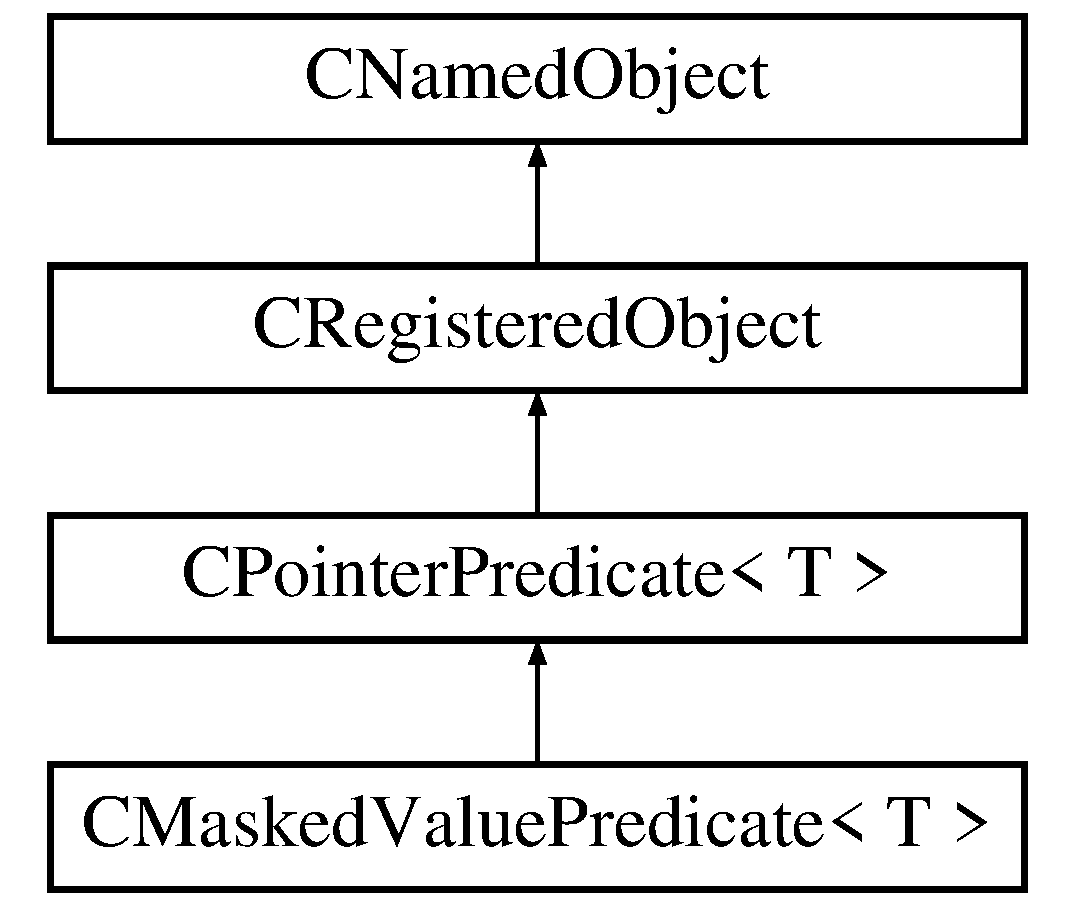
\includegraphics[height=4cm]{classCMaskedValuePredicate}
\end{center}
\end{figure}
\subsection*{Public Methods}
\begin{CompactItemize}
\item 
{\bf CMasked\-Value\-Predicate} (T am\_\-TValue, T am\_\-TMask={\bf COS\_\-ALLBITS})
\item 
{\bf CMasked\-Value\-Predicate} (const string \&r\-Name, T am\_\-TValue, T am\_\-TMask={\bf COS\_\-ALLBITS})
\item 
{\bf CMasked\-Value\-Predicate} (const char $\ast$p\-Name, T am\_\-TValue, T am\_\-TMask={\bf COS\_\-ALLBITS})
\item 
{\bf $\sim$CMasked\-Value\-Predicate} ()
\item 
int {\bf operator==} (const CMasked\-Value\-Predicate$<$ T $>$ \&a\-CMasked\-Value\-Predicate) const
\item 
T {\bf get\-Mask} () const
\item 
T {\bf get\-Value} () const
\item 
virtual bool {\bf operator()} (T n\-Value)
\item 
virtual string {\bf Describe\-Self} ()
\end{CompactItemize}
\subsection*{Protected Methods}
\begin{CompactItemize}
\item 
void {\bf set\-Mask} (const T am\_\-TMask)
\item 
void {\bf set\-Value} (const T am\_\-TValue)
\end{CompactItemize}
\subsection*{Private Methods}
\begin{CompactItemize}
\item 
{\bf CMasked\-Value\-Predicate} (const CMasked\-Value\-Predicate$<$ T $>$ \&a\-CMasked\-Value\-Predicate)
\item 
CMasked\-Value\-Predicate$<$ T $>$ {\bf operator=} (const CMasked\-Value\-Predicate$<$ T $>$ \&a\-CMasked\-Value\-Predicate)
\end{CompactItemize}
\subsection*{Private Attributes}
\begin{CompactItemize}
\item 
T {\bf m\_\-TValue}
\item 
T {\bf m\_\-TMask}
\end{CompactItemize}
\subsubsection*{template$<$typename T$>$ class CMasked\-Value\-Predicate$<$ T $>$}



\subsection{Constructor \& Destructor Documentation}
\index{CMaskedValuePredicate@{CMasked\-Value\-Predicate}!CMaskedValuePredicate@{CMaskedValuePredicate}}
\index{CMaskedValuePredicate@{CMaskedValuePredicate}!CMaskedValuePredicate@{CMasked\-Value\-Predicate}}
\subsubsection{\setlength{\rightskip}{0pt plus 5cm}template$<$typename T$>$ CMasked\-Value\-Predicate$<$ T $>$::CMasked\-Value\-Predicate (T {\em am\_\-TValue}, T {\em am\_\-TMask} = {\bf COS\_\-ALLBITS})\hspace{0.3cm}{\tt  [inline]}}\label{classCMaskedValuePredicate_a0}


The predicate mask \index{CMaskedValuePredicate@{CMasked\-Value\-Predicate}!CMaskedValuePredicate@{CMaskedValuePredicate}}
\index{CMaskedValuePredicate@{CMaskedValuePredicate}!CMaskedValuePredicate@{CMasked\-Value\-Predicate}}
\subsubsection{\setlength{\rightskip}{0pt plus 5cm}template$<$typename T$>$ CMasked\-Value\-Predicate$<$ T $>$::CMasked\-Value\-Predicate (const string \& {\em r\-Name}, T {\em am\_\-TValue}, T {\em am\_\-TMask} = {\bf COS\_\-ALLBITS})\hspace{0.3cm}{\tt  [inline]}}\label{classCMaskedValuePredicate_a1}


\index{CMaskedValuePredicate@{CMasked\-Value\-Predicate}!CMaskedValuePredicate@{CMaskedValuePredicate}}
\index{CMaskedValuePredicate@{CMaskedValuePredicate}!CMaskedValuePredicate@{CMasked\-Value\-Predicate}}
\subsubsection{\setlength{\rightskip}{0pt plus 5cm}template$<$typename T$>$ CMasked\-Value\-Predicate$<$ T $>$::CMasked\-Value\-Predicate (const char $\ast$ {\em p\-Name}, T {\em am\_\-TValue}, T {\em am\_\-TMask} = {\bf COS\_\-ALLBITS})\hspace{0.3cm}{\tt  [inline]}}\label{classCMaskedValuePredicate_a2}


\index{CMaskedValuePredicate@{CMasked\-Value\-Predicate}!~CMaskedValuePredicate@{$\sim$CMaskedValuePredicate}}
\index{~CMaskedValuePredicate@{$\sim$CMaskedValuePredicate}!CMaskedValuePredicate@{CMasked\-Value\-Predicate}}
\subsubsection{\setlength{\rightskip}{0pt plus 5cm}template$<$typename T$>$ CMasked\-Value\-Predicate$<$ T $>$::$\sim$CMasked\-Value\-Predicate ()\hspace{0.3cm}{\tt  [inline]}}\label{classCMaskedValuePredicate_a3}


\index{CMaskedValuePredicate@{CMasked\-Value\-Predicate}!CMaskedValuePredicate@{CMaskedValuePredicate}}
\index{CMaskedValuePredicate@{CMaskedValuePredicate}!CMaskedValuePredicate@{CMasked\-Value\-Predicate}}
\subsubsection{\setlength{\rightskip}{0pt plus 5cm}template$<$typename T$>$ CMasked\-Value\-Predicate$<$ T $>$::CMasked\-Value\-Predicate (const CMasked\-Value\-Predicate$<$ T $>$ \& {\em a\-CMasked\-Value\-Predicate})\hspace{0.3cm}{\tt  [private]}}\label{classCMaskedValuePredicate_c0}




\subsection{Member Function Documentation}
\index{CMaskedValuePredicate@{CMasked\-Value\-Predicate}!DescribeSelf@{DescribeSelf}}
\index{DescribeSelf@{DescribeSelf}!CMaskedValuePredicate@{CMasked\-Value\-Predicate}}
\subsubsection{\setlength{\rightskip}{0pt plus 5cm}template$<$typename T$>$ string CMasked\-Value\-Predicate$<$ T $>$::Describe\-Self ()\hspace{0.3cm}{\tt  [virtual]}}\label{classCMaskedValuePredicate_a8}


Operation Type: Selector

Purpose: Returns a string with the following information: 1 - m\_\-TMask 2 - m\_\-TValue 

Implements {\bf CPointer\-Predicate$<$ T $>$} {\rm (p.\,\pageref{classCPointerPredicate_a6})}.

Definition at line 315 of file CMasked\-Value\-Predicate.cpp.

References CMasked\-Value\-Predicate$<$ T $>$::m\_\-TMask, and CMasked\-Value\-Predicate$<$ T $>$::m\_\-TValue.\index{CMaskedValuePredicate@{CMasked\-Value\-Predicate}!getMask@{getMask}}
\index{getMask@{getMask}!CMaskedValuePredicate@{CMasked\-Value\-Predicate}}
\subsubsection{\setlength{\rightskip}{0pt plus 5cm}template$<$typename T$>$ T CMasked\-Value\-Predicate$<$ T $>$::get\-Mask () const\hspace{0.3cm}{\tt  [inline]}}\label{classCMaskedValuePredicate_a5}




Definition at line 352 of file CMasked\-Value\-Predicate.h.\index{CMaskedValuePredicate@{CMasked\-Value\-Predicate}!getValue@{getValue}}
\index{getValue@{getValue}!CMaskedValuePredicate@{CMasked\-Value\-Predicate}}
\subsubsection{\setlength{\rightskip}{0pt plus 5cm}template$<$typename T$>$ T CMasked\-Value\-Predicate$<$ T $>$::get\-Value () const\hspace{0.3cm}{\tt  [inline]}}\label{classCMaskedValuePredicate_a6}




Definition at line 357 of file CMasked\-Value\-Predicate.h.\index{CMaskedValuePredicate@{CMasked\-Value\-Predicate}!operator()@{operator()}}
\index{operator()@{operator()}!CMaskedValuePredicate@{CMasked\-Value\-Predicate}}
\subsubsection{\setlength{\rightskip}{0pt plus 5cm}template$<$typename T$>$ bool CMasked\-Value\-Predicate$<$ T $>$::operator() (T {\em n\-Value})\hspace{0.3cm}{\tt  [virtual]}}\label{classCMaskedValuePredicate_a7}


Operation Type: Override behavior

Purpose: Returns true if (n\-Value \& m\_\-TMask) == m\_\-TValue 

Implements {\bf CPointer\-Predicate$<$ T $>$} {\rm (p.\,\pageref{classCPointerPredicate_a5})}.

Definition at line 296 of file CMasked\-Value\-Predicate.cpp.

References CMasked\-Value\-Predicate$<$ T $>$::m\_\-TMask, and CMasked\-Value\-Predicate$<$ T $>$::m\_\-TValue.\index{CMaskedValuePredicate@{CMasked\-Value\-Predicate}!operator=@{operator=}}
\index{operator=@{operator=}!CMaskedValuePredicate@{CMasked\-Value\-Predicate}}
\subsubsection{\setlength{\rightskip}{0pt plus 5cm}template$<$typename T$>$ CMasked\-Value\-Predicate$<$T$>$ CMasked\-Value\-Predicate$<$ T $>$::operator= (const CMasked\-Value\-Predicate$<$ T $>$ \& {\em a\-CMasked\-Value\-Predicate})\hspace{0.3cm}{\tt  [private]}}\label{classCMaskedValuePredicate_c1}


\index{CMaskedValuePredicate@{CMasked\-Value\-Predicate}!operator==@{operator==}}
\index{operator==@{operator==}!CMaskedValuePredicate@{CMasked\-Value\-Predicate}}
\subsubsection{\setlength{\rightskip}{0pt plus 5cm}template$<$typename T$>$ int CMasked\-Value\-Predicate$<$ T $>$::operator== (const CMasked\-Value\-Predicate$<$ T $>$ \& {\em a\-CMasked\-Value\-Predicate}) const\hspace{0.3cm}{\tt  [inline]}}\label{classCMaskedValuePredicate_a4}




Definition at line 333 of file CMasked\-Value\-Predicate.h.

References CMasked\-Value\-Predicate$<$ T $>$::m\_\-TMask, CMasked\-Value\-Predicate$<$ T $>$::m\_\-TValue, and CPointer\-Predicate$<$ T $>$::operator==().\index{CMaskedValuePredicate@{CMasked\-Value\-Predicate}!setMask@{setMask}}
\index{setMask@{setMask}!CMaskedValuePredicate@{CMasked\-Value\-Predicate}}
\subsubsection{\setlength{\rightskip}{0pt plus 5cm}template$<$typename T$>$ void CMasked\-Value\-Predicate$<$ T $>$::set\-Mask (const T {\em am\_\-TMask})\hspace{0.3cm}{\tt  [inline, protected]}}\label{classCMaskedValuePredicate_b0}




Definition at line 365 of file CMasked\-Value\-Predicate.h.\index{CMaskedValuePredicate@{CMasked\-Value\-Predicate}!setValue@{setValue}}
\index{setValue@{setValue}!CMaskedValuePredicate@{CMasked\-Value\-Predicate}}
\subsubsection{\setlength{\rightskip}{0pt plus 5cm}template$<$typename T$>$ void CMasked\-Value\-Predicate$<$ T $>$::set\-Value (const T {\em am\_\-TValue})\hspace{0.3cm}{\tt  [inline, protected]}}\label{classCMaskedValuePredicate_b1}




Definition at line 370 of file CMasked\-Value\-Predicate.h.

\subsection{Member Data Documentation}
\index{CMaskedValuePredicate@{CMasked\-Value\-Predicate}!m_TMask@{m\_\-TMask}}
\index{m_TMask@{m\_\-TMask}!CMaskedValuePredicate@{CMasked\-Value\-Predicate}}
\subsubsection{\setlength{\rightskip}{0pt plus 5cm}template$<$typename T$>$ T CMasked\-Value\-Predicate$<$ T $>$::m\_\-TMask\hspace{0.3cm}{\tt  [private]}}\label{classCMaskedValuePredicate_o1}


The predicate value 

Definition at line 304 of file CMasked\-Value\-Predicate.h.

Referenced by CMasked\-Value\-Predicate$<$ T $>$::Describe\-Self(), CMasked\-Value\-Predicate$<$ T $>$::operator()(), and CMasked\-Value\-Predicate$<$ T $>$::operator==().\index{CMaskedValuePredicate@{CMasked\-Value\-Predicate}!m_TValue@{m\_\-TValue}}
\index{m_TValue@{m\_\-TValue}!CMaskedValuePredicate@{CMasked\-Value\-Predicate}}
\subsubsection{\setlength{\rightskip}{0pt plus 5cm}template$<$typename T$>$ T CMasked\-Value\-Predicate$<$ T $>$::m\_\-TValue\hspace{0.3cm}{\tt  [private]}}\label{classCMaskedValuePredicate_o0}




Definition at line 303 of file CMasked\-Value\-Predicate.h.

Referenced by CMasked\-Value\-Predicate$<$ T $>$::Describe\-Self(), CMasked\-Value\-Predicate$<$ T $>$::operator()(), and CMasked\-Value\-Predicate$<$ T $>$::operator==().

The documentation for this class was generated from the following files:\begin{CompactItemize}
\item 
{\bf CMasked\-Value\-Predicate.h}\item 
{\bf CMasked\-Value\-Predicate.cpp}\end{CompactItemize}

\section{Match\-All  Class Reference}
\label{classMatchAll}\index{MatchAll@{Match\-All}}
{\tt \#include $<$CBuffer\-Monitor.h$>$}

\subsection*{Public Methods}
\begin{CompactItemize}
\item 
{\bf Match\-All} (string \&r\-URL, int n\-Tag, int n\-Mask)
\item 
virtual bool {\bf operator()} (struct {\bf Link\-Info} l)
\end{CompactItemize}
\subsection*{Private Attributes}
\begin{CompactItemize}
\item 
string {\bf m\_\-s\-URL}
\item 
int {\bf m\_\-n\-Tag}
\item 
int {\bf m\_\-n\-Mask}
\end{CompactItemize}


\subsection{Constructor \& Destructor Documentation}
\index{MatchAll@{Match\-All}!MatchAll@{MatchAll}}
\index{MatchAll@{MatchAll}!MatchAll@{Match\-All}}
\subsubsection{\setlength{\rightskip}{0pt plus 5cm}Match\-All::Match\-All (string \& {\em r\-URL}, int {\em n\-Tag}, int {\em n\-Mask})\hspace{0.3cm}{\tt  [inline]}}\label{classMatchAll_a0}




Definition at line 360 of file CBuffer\-Monitor.h.

References m\_\-n\-Mask, m\_\-n\-Tag, and m\_\-s\-URL.

\subsection{Member Function Documentation}
\index{MatchAll@{Match\-All}!operator()@{operator()}}
\index{operator()@{operator()}!MatchAll@{Match\-All}}
\subsubsection{\setlength{\rightskip}{0pt plus 5cm}virtual bool Match\-All::operator() (struct {\bf Link\-Info} {\em l})\hspace{0.3cm}{\tt  [inline, virtual]}}\label{classMatchAll_a1}




Definition at line 364 of file CBuffer\-Monitor.h.

References m\_\-n\-Mask, m\_\-n\-Tag, m\_\-s\-URL, Link\-Info::Mask, Link\-Info::Tag, and Link\-Info::URL.

\subsection{Member Data Documentation}
\index{MatchAll@{Match\-All}!m_nMask@{m\_\-nMask}}
\index{m_nMask@{m\_\-nMask}!MatchAll@{Match\-All}}
\subsubsection{\setlength{\rightskip}{0pt plus 5cm}int Match\-All::m\_\-n\-Mask\hspace{0.3cm}{\tt  [private]}}\label{classMatchAll_o2}




Definition at line 358 of file CBuffer\-Monitor.h.

Referenced by Match\-All(), and operator()().\index{MatchAll@{Match\-All}!m_nTag@{m\_\-nTag}}
\index{m_nTag@{m\_\-nTag}!MatchAll@{Match\-All}}
\subsubsection{\setlength{\rightskip}{0pt plus 5cm}int Match\-All::m\_\-n\-Tag\hspace{0.3cm}{\tt  [private]}}\label{classMatchAll_o1}




Definition at line 357 of file CBuffer\-Monitor.h.

Referenced by Match\-All(), and operator()().\index{MatchAll@{Match\-All}!m_sURL@{m\_\-sURL}}
\index{m_sURL@{m\_\-sURL}!MatchAll@{Match\-All}}
\subsubsection{\setlength{\rightskip}{0pt plus 5cm}string Match\-All::m\_\-s\-URL\hspace{0.3cm}{\tt  [private]}}\label{classMatchAll_o0}




Definition at line 356 of file CBuffer\-Monitor.h.

Referenced by Match\-All(), and operator()().

The documentation for this class was generated from the following file:\begin{CompactItemize}
\item 
{\bf CBuffer\-Monitor.h}\end{CompactItemize}

\section{Match\-URL  Class Reference}
\label{classMatchURL}\index{MatchURL@{Match\-URL}}
{\tt \#include $<$CBuffer\-Monitor.h$>$}

\subsection*{Public Methods}
\begin{CompactItemize}
\item 
{\bf Match\-URL} (string \&r\-URL)
\item 
bool {\bf operator()} (struct {\bf Link\-Info} l)
\end{CompactItemize}
\subsection*{Private Attributes}
\begin{CompactItemize}
\item 
string {\bf m\_\-s\-URL}
\end{CompactItemize}


\subsection{Constructor \& Destructor Documentation}
\index{MatchURL@{Match\-URL}!MatchURL@{MatchURL}}
\index{MatchURL@{MatchURL}!MatchURL@{Match\-URL}}
\subsubsection{\setlength{\rightskip}{0pt plus 5cm}Match\-URL::Match\-URL (string \& {\em r\-URL})\hspace{0.3cm}{\tt  [inline]}}\label{classMatchURL_a0}




Definition at line 348 of file CBuffer\-Monitor.h.

References m\_\-s\-URL.

\subsection{Member Function Documentation}
\index{MatchURL@{Match\-URL}!operator()@{operator()}}
\index{operator()@{operator()}!MatchURL@{Match\-URL}}
\subsubsection{\setlength{\rightskip}{0pt plus 5cm}bool Match\-URL::operator() (struct {\bf Link\-Info} {\em l})\hspace{0.3cm}{\tt  [inline]}}\label{classMatchURL_a1}




Definition at line 350 of file CBuffer\-Monitor.h.

References m\_\-s\-URL, and Link\-Info::URL.

\subsection{Member Data Documentation}
\index{MatchURL@{Match\-URL}!m_sURL@{m\_\-sURL}}
\index{m_sURL@{m\_\-sURL}!MatchURL@{Match\-URL}}
\subsubsection{\setlength{\rightskip}{0pt plus 5cm}string Match\-URL::m\_\-s\-URL\hspace{0.3cm}{\tt  [private]}}\label{classMatchURL_o0}




Definition at line 346 of file CBuffer\-Monitor.h.

Referenced by Match\-URL(), and operator()().

The documentation for this class was generated from the following file:\begin{CompactItemize}
\item 
{\bf CBuffer\-Monitor.h}\end{CompactItemize}

\section{CNamed\-Object  Class Reference}
\label{classCNamedObject}\index{CNamedObject@{CNamed\-Object}}
{\tt \#include $<$CNamed\-Object.h$>$}

Inheritance diagram for CNamed\-Object::\begin{figure}[H]
\begin{center}
\leavevmode
\includegraphics[height=2.46696cm]{classCNamedObject}
\end{center}
\end{figure}
\subsection*{Public Methods}
\begin{CompactItemize}
\item 
{\bf CNamed\-Object} ()
\item 
{\bf CNamed\-Object} (string am\_\-s\-Name)
\item 
virtual {\bf $\sim$CNamed\-Object} ()
\item 
CNamed\-Object \& {\bf operator=} (const CNamed\-Object \&rhs)
\item 
int {\bf operator==} (const CNamed\-Object \&rhs) const
\item 
string {\bf get\-Class\-Path} () const
\item 
const string {\bf get\-Name} () const
\item 
unsigned int {\bf get\-Auto\-Index} () const
\begin{CompactList}\small\item\em $<$ Return value of auto naming index.\item\end{CompactList}\item 
virtual string {\bf Describe\-Self} ()
\end{CompactItemize}
\subsection*{Protected Methods}
\begin{CompactItemize}
\item 
void {\bf set\-Class\-Path} (const string am\_\-s\-Class\-Path)
\item 
void {\bf set\-Auto\-Index} (unsigned n\-New)
\item 
virtual void {\bf Append\-Class\-Info} ()
\end{CompactItemize}
\subsection*{Static Protected Methods}
\begin{CompactItemize}
\item 
string {\bf Get\-Auto\-Name} (const string \&r\-Base)
\begin{CompactList}\small\item\em Assign default name.\item\end{CompactList}\end{CompactItemize}
\subsection*{Private Attributes}
\begin{CompactItemize}
\item 
string {\bf m\_\-s\-Name}
\item 
string {\bf m\_\-s\-Class\-Path}
\end{CompactItemize}
\subsection*{Static Private Attributes}
\begin{CompactItemize}
\item 
unsigned int {\bf m\_\-n\-Auto\-Index}
\begin{CompactList}\small\item\em Used to name autonamed objects.\item\end{CompactList}\end{CompactItemize}


\subsection{Detailed Description}
Definition of a named object. Named objects are objects with a name and class path. The class path describes what type the object derived from CNamed\-Object actually is. That type is determined by Append\-Class() which uses RTTI and is called each time CNamed\-Object (or anything derived from it) is instantiated. 



Definition at line 314 of file CNamed\-Object.h.

\subsection{Constructor \& Destructor Documentation}
\index{CNamedObject@{CNamed\-Object}!CNamedObject@{CNamedObject}}
\index{CNamedObject@{CNamedObject}!CNamedObject@{CNamed\-Object}}
\subsubsection{\setlength{\rightskip}{0pt plus 5cm}CNamed\-Object::CNamed\-Object ()\hspace{0.3cm}{\tt  [inline]}}\label{classCNamedObject_a0}




Definition at line 323 of file CNamed\-Object.h.

References Append\-Class\-Info(), Get\-Auto\-Name(), and m\_\-s\-Name.\index{CNamedObject@{CNamed\-Object}!CNamedObject@{CNamedObject}}
\index{CNamedObject@{CNamedObject}!CNamedObject@{CNamed\-Object}}
\subsubsection{\setlength{\rightskip}{0pt plus 5cm}CNamed\-Object::CNamed\-Object (string {\em am\_\-s\-Name})\hspace{0.3cm}{\tt  [inline]}}\label{classCNamedObject_a1}




Definition at line 328 of file CNamed\-Object.h.

References Append\-Class\-Info(), and m\_\-s\-Name.\index{CNamedObject@{CNamed\-Object}!~CNamedObject@{$\sim$CNamedObject}}
\index{~CNamedObject@{$\sim$CNamedObject}!CNamedObject@{CNamed\-Object}}
\subsubsection{\setlength{\rightskip}{0pt plus 5cm}virtual CNamed\-Object::$\sim$CNamed\-Object ()\hspace{0.3cm}{\tt  [inline, virtual]}}\label{classCNamedObject_a2}




Definition at line 333 of file CNamed\-Object.h.

\subsection{Member Function Documentation}
\index{CNamedObject@{CNamed\-Object}!AppendClassInfo@{AppendClassInfo}}
\index{AppendClassInfo@{AppendClassInfo}!CNamedObject@{CNamed\-Object}}
\subsubsection{\setlength{\rightskip}{0pt plus 5cm}void CNamed\-Object::Append\-Class\-Info ()\hspace{0.3cm}{\tt  [protected, virtual]}}\label{classCNamedObject_b2}


Appends class information to m\_\-s\-Class\-Path. The information consists of the class hierarchy of the object being created. 

Definition at line 304 of file CNamed\-Object.cpp.

References m\_\-s\-Class\-Path.

Referenced by CBuffer\-Reactor$<$ T $>$::CBuffer\-Reactor(), CClassified\-Object\-Registry::CClassified\-Object\-Registry(), CEvent::CEvent(), CEvent\-Monitor::CEvent\-Monitor(), CFd\-Monitor::CFd\-Monitor(), CFd\-Reactor::CFd\-Reactor(), CFile\-Event::CFile\-Event(), CFile\-Event\-Reactor::CFile\-Event\-Reactor(), CLocation\-Reactor$<$ T $>$::CLocation\-Reactor(), CNamed\-Object(), CObject\-Registry::CObject\-Registry(), CReactor::CReactor(), CRegistered\-Object::CRegistered\-Object(), and CTimer\-Monitor::CTimer\-Monitor().\index{CNamedObject@{CNamed\-Object}!DescribeSelf@{DescribeSelf}}
\index{DescribeSelf@{DescribeSelf}!CNamedObject@{CNamed\-Object}}
\subsubsection{\setlength{\rightskip}{0pt plus 5cm}string CNamed\-Object::Describe\-Self ()\hspace{0.3cm}{\tt  [virtual]}}\label{classCNamedObject_a8}


Describes the named object. The information given is the object type given by m\_\-s\-Class\-Path, and the object name. 

Reimplemented in {\bf CBuffer\-Event$<$ T $>$} {\rm (p.\,\pageref{classCBufferEvent_a14})}, {\bf CBuffer\-Monitor$<$ T $>$} {\rm (p.\,\pageref{classCBufferMonitor_a17})}, {\bf CChanged\-Predicate$<$ T $>$} {\rm (p.\,\pageref{classCChangedPredicate_a7})}, {\bf CClassified\-Object\-Registry} {\rm (p.\,\pageref{classCClassifiedObjectRegistry_a11})}, {\bf CEvent} {\rm (p.\,\pageref{classCEvent_a16})}, {\bf CFd\-Monitor} {\rm (p.\,\pageref{classCFdMonitor_a12})}, {\bf CFile\-Event} {\rm (p.\,\pageref{classCFileEvent_a19})}, {\bf CLocation\-Event$<$ T $>$} {\rm (p.\,\pageref{classCLocationEvent_a10})}, {\bf CLocation\-Monitor$<$ T $>$} {\rm (p.\,\pageref{classCLocationMonitor_a11})}, {\bf CMasked\-Value\-Predicate$<$ T $>$} {\rm (p.\,\pageref{classCMaskedValuePredicate_a8})}, {\bf CObject\-Registry} {\rm (p.\,\pageref{classCObjectRegistry_a9})}, {\bf CPointer\-Predicate$<$ T $>$} {\rm (p.\,\pageref{classCPointerPredicate_a6})}, {\bf CServer\-Connection\-Event} {\rm (p.\,\pageref{classCServerConnectionEvent_a14})}, {\bf CServer\-Instance} {\rm (p.\,\pageref{classCServerInstance_a11})}, {\bf CServer\-Monitor} {\rm (p.\,\pageref{classCServerMonitor_a8})}, {\bf CTimer\-Event} {\rm (p.\,\pageref{classCTimerEvent_a12})}, {\bf CTimer\-Monitor} {\rm (p.\,\pageref{classCTimerMonitor_a10})}, {\bf CBuffer\-Event$<$ U $>$} {\rm (p.\,\pageref{classCBufferEvent_a14})}, and {\bf CBuffer\-Monitor$<$ U $>$} {\rm (p.\,\pageref{classCBufferMonitor_a17})}.

Definition at line 316 of file CNamed\-Object.cpp.

References m\_\-s\-Class\-Path, and m\_\-s\-Name.

Referenced by CTimer\-Monitor::Describe\-Self(), CObject\-Registry::Describe\-Self(), CLocation\-Monitor$<$ T $>$::Describe\-Self(), CFd\-Monitor::Describe\-Self(), CEvent::Describe\-Self(), CClassified\-Object\-Registry::Describe\-Self(), and CBuffer\-Monitor$<$ T $>$::Describe\-Self().\index{CNamedObject@{CNamed\-Object}!getAutoIndex@{getAutoIndex}}
\index{getAutoIndex@{getAutoIndex}!CNamedObject@{CNamed\-Object}}
\subsubsection{\setlength{\rightskip}{0pt plus 5cm}unsigned int CNamed\-Object::get\-Auto\-Index () const\hspace{0.3cm}{\tt  [inline]}}\label{classCNamedObject_a7}


$<$ Return value of auto naming index.



Definition at line 364 of file CNamed\-Object.h.

References m\_\-n\-Auto\-Index.\index{CNamedObject@{CNamed\-Object}!GetAutoName@{GetAutoName}}
\index{GetAutoName@{GetAutoName}!CNamedObject@{CNamed\-Object}}
\subsubsection{\setlength{\rightskip}{0pt plus 5cm}string CNamed\-Object::Get\-Auto\-Name (const string \& {\em r\-Base})\hspace{0.3cm}{\tt  [static, protected]}}\label{classCNamedObject_e0}


Assign default name.

Allocate a name for an object given some generic base name.  The final name is of the form: Base\-Name(m\_\-n\-Auto\-Index). 

Reimplemented in {\bf CEvent\-Monitor} {\rm (p.\,\pageref{classCEventMonitor_e0})}, and {\bf CPointer\-Predicate$<$ T $>$} {\rm (p.\,\pageref{classCPointerPredicate_e0})}.

Definition at line 330 of file CNamed\-Object.cpp.

References m\_\-n\-Auto\-Index.

Referenced by CFile\-Event::CFile\-Event(), and CNamed\-Object().\index{CNamedObject@{CNamed\-Object}!getClassPath@{getClassPath}}
\index{getClassPath@{getClassPath}!CNamedObject@{CNamed\-Object}}
\subsubsection{\setlength{\rightskip}{0pt plus 5cm}string CNamed\-Object::get\-Class\-Path () const\hspace{0.3cm}{\tt  [inline]}}\label{classCNamedObject_a5}




Definition at line 354 of file CNamed\-Object.h.

References m\_\-s\-Class\-Path.\index{CNamedObject@{CNamed\-Object}!getName@{getName}}
\index{getName@{getName}!CNamedObject@{CNamed\-Object}}
\subsubsection{\setlength{\rightskip}{0pt plus 5cm}const string CNamed\-Object::get\-Name () const\hspace{0.3cm}{\tt  [inline]}}\label{classCNamedObject_a6}




Definition at line 360 of file CNamed\-Object.h.

References m\_\-s\-Name.

Referenced by CObject\-Registry::Add(), CObject\-Registry::Remove(), and CClassified\-Object\-Registry::Remove().\index{CNamedObject@{CNamed\-Object}!operator=@{operator=}}
\index{operator=@{operator=}!CNamedObject@{CNamed\-Object}}
\subsubsection{\setlength{\rightskip}{0pt plus 5cm}CNamed\-Object\& CNamed\-Object::operator= (const CNamed\-Object \& {\em rhs})\hspace{0.3cm}{\tt  [inline]}}\label{classCNamedObject_a3}




Definition at line 337 of file CNamed\-Object.h.

References m\_\-s\-Class\-Path, and m\_\-s\-Name.\index{CNamedObject@{CNamed\-Object}!operator==@{operator==}}
\index{operator==@{operator==}!CNamedObject@{CNamed\-Object}}
\subsubsection{\setlength{\rightskip}{0pt plus 5cm}int CNamed\-Object::operator== (const CNamed\-Object \& {\em rhs}) const\hspace{0.3cm}{\tt  [inline]}}\label{classCNamedObject_a4}




Definition at line 345 of file CNamed\-Object.h.

References m\_\-s\-Class\-Path, and m\_\-s\-Name.

Referenced by CRegistered\-Object::operator==().\index{CNamedObject@{CNamed\-Object}!setAutoIndex@{setAutoIndex}}
\index{setAutoIndex@{setAutoIndex}!CNamedObject@{CNamed\-Object}}
\subsubsection{\setlength{\rightskip}{0pt plus 5cm}void CNamed\-Object::set\-Auto\-Index (unsigned {\em n\-New})\hspace{0.3cm}{\tt  [inline, protected]}}\label{classCNamedObject_b1}




Definition at line 378 of file CNamed\-Object.h.

References m\_\-n\-Auto\-Index.\index{CNamedObject@{CNamed\-Object}!setClassPath@{setClassPath}}
\index{setClassPath@{setClassPath}!CNamedObject@{CNamed\-Object}}
\subsubsection{\setlength{\rightskip}{0pt plus 5cm}void CNamed\-Object::set\-Class\-Path (const string {\em am\_\-s\-Class\-Path})\hspace{0.3cm}{\tt  [inline, protected]}}\label{classCNamedObject_b0}




Definition at line 374 of file CNamed\-Object.h.

References m\_\-s\-Class\-Path.

\subsection{Member Data Documentation}
\index{CNamedObject@{CNamed\-Object}!m_nAutoIndex@{m\_\-nAutoIndex}}
\index{m_nAutoIndex@{m\_\-nAutoIndex}!CNamedObject@{CNamed\-Object}}
\subsubsection{\setlength{\rightskip}{0pt plus 5cm}unsigned int CNamed\-Object::m\_\-n\-Auto\-Index\hspace{0.3cm}{\tt  [static, private]}}\label{classCNamedObject_r0}


Used to name autonamed objects.

Named\-Object.cpp Base class for all objects in the event management system.

Author: Jason Venema NSCL Michigan State University East Lansing, MI 48824-1321 mailto:{\tt venemaja@msu.edu} 

Reimplemented in {\bf CEvent\-Monitor} {\rm (p.\,\pageref{classCEventMonitor_r0})}, and {\bf CPointer\-Predicate$<$ T $>$} {\rm (p.\,\pageref{classCPointerPredicate_r0})}.

Referenced by get\-Auto\-Index(), Get\-Auto\-Name(), and set\-Auto\-Index().\index{CNamedObject@{CNamed\-Object}!m_sClassPath@{m\_\-sClassPath}}
\index{m_sClassPath@{m\_\-sClassPath}!CNamedObject@{CNamed\-Object}}
\subsubsection{\setlength{\rightskip}{0pt plus 5cm}string CNamed\-Object::m\_\-s\-Class\-Path\hspace{0.3cm}{\tt  [private]}}\label{classCNamedObject_o1}


The class path of the object 

Definition at line 317 of file CNamed\-Object.h.

Referenced by Append\-Class\-Info(), Describe\-Self(), get\-Class\-Path(), operator=(), operator==(), and set\-Class\-Path().\index{CNamedObject@{CNamed\-Object}!m_sName@{m\_\-sName}}
\index{m_sName@{m\_\-sName}!CNamedObject@{CNamed\-Object}}
\subsubsection{\setlength{\rightskip}{0pt plus 5cm}string CNamed\-Object::m\_\-s\-Name\hspace{0.3cm}{\tt  [private]}}\label{classCNamedObject_o0}


The name of the object 

Definition at line 316 of file CNamed\-Object.h.

Referenced by CNamed\-Object(), Describe\-Self(), get\-Name(), operator=(), and operator==().

The documentation for this class was generated from the following files:\begin{CompactItemize}
\item 
{\bf CNamed\-Object.h}\item 
{\bf CNamed\-Object.cpp}\end{CompactItemize}

\section{CNo\-Such\-Link\-Exception  Class Reference}
\label{classCNoSuchLinkException}\index{CNoSuchLinkException@{CNo\-Such\-Link\-Exception}}
{\tt \#include $<$CNo\-Such\-Link\-Exception.h$>$}

Inheritance diagram for CNo\-Such\-Link\-Exception::\begin{figure}[H]
\begin{center}
\leavevmode
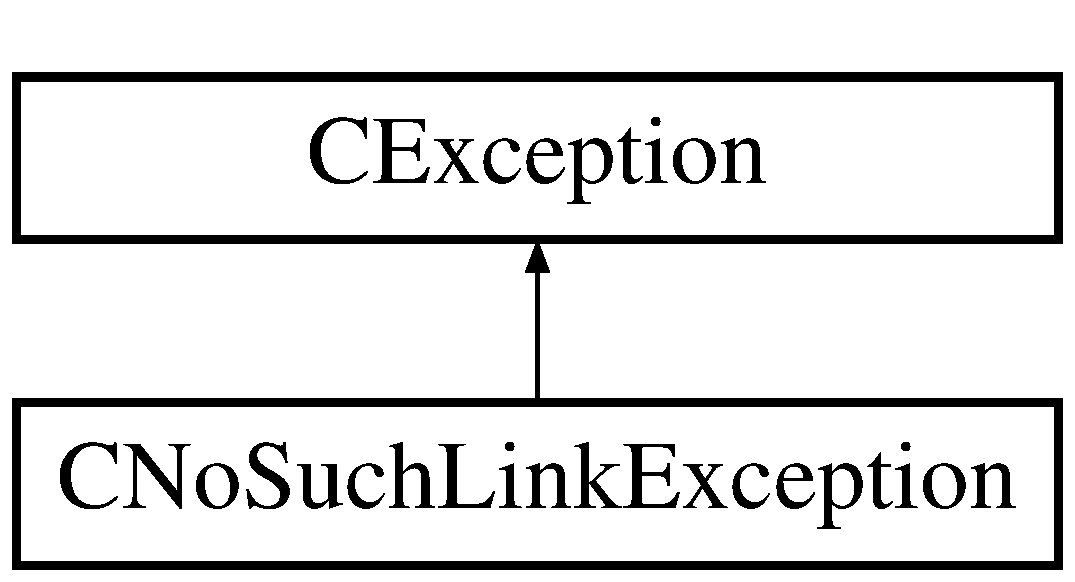
\includegraphics[height=2cm]{classCNoSuchLinkException}
\end{center}
\end{figure}
\subsection*{Public Methods}
\begin{CompactItemize}
\item 
{\bf CNo\-Such\-Link\-Exception} (const char $\ast$p\-Doing, const char $\ast$p\-Name)
\item 
{\bf CNo\-Such\-Link\-Exception} (const char $\ast$p\-Doing, const string \&r\-Name)
\item 
{\bf CNo\-Such\-Link\-Exception} (const string \&r\-Doing, const char $\ast$p\-Name)
\item 
{\bf CNo\-Such\-Link\-Exception} (const string \&r\-Doing, const string \&r\-Name)
\item 
{\bf CNo\-Such\-Link\-Exception} (const string \&r\-Doing, int n\-Id)
\item 
{\bf CNo\-Such\-Link\-Exception} (const char $\ast$p\-Doing, int n\-Id)
\item 
virtual {\bf $\sim$CNo\-Such\-Link\-Exception} ()
\item 
{\bf CNo\-Such\-Link\-Exception} (const CNo\-Such\-Link\-Exception \&a\-CNo\-Such\-Link\-Exception)
\item 
CNo\-Such\-Link\-Exception {\bf operator=} (const CNo\-Such\-Link\-Exception \&a\-CNo\-Such\-Link\-Exception)
\item 
int {\bf operator==} (const CNo\-Such\-Link\-Exception \&a\-CNo\-Such\-Link\-Exception)
\item 
string {\bf get\-Name} () const
\item 
void {\bf set\-Name} (string am\_\-s\-Name)
\item 
virtual const char $\ast$ {\bf Reason\-Text} () const
\end{CompactItemize}
\subsection*{Protected Methods}
\begin{CompactItemize}
\item 
void {\bf Update\-Reason\-Text} ()
\end{CompactItemize}
\subsection*{Private Attributes}
\begin{CompactItemize}
\item 
string {\bf m\_\-s\-Name}
\item 
int {\bf m\_\-n\-Id}
\item 
bool {\bf m\_\-f\-Name}
\item 
string {\bf m\_\-s\-Reason\-Text}
\end{CompactItemize}


\subsection{Constructor \& Destructor Documentation}
\index{CNoSuchLinkException@{CNo\-Such\-Link\-Exception}!CNoSuchLinkException@{CNoSuchLinkException}}
\index{CNoSuchLinkException@{CNoSuchLinkException}!CNoSuchLinkException@{CNo\-Such\-Link\-Exception}}
\subsubsection{\setlength{\rightskip}{0pt plus 5cm}CNo\-Such\-Link\-Exception::CNo\-Such\-Link\-Exception (const char $\ast$ {\em p\-Doing}, const char $\ast$ {\em p\-Name})\hspace{0.3cm}{\tt  [inline]}}\label{classCNoSuchLinkException_a0}




Definition at line 301 of file CNo\-Such\-Link\-Exception.h.

References m\_\-s\-Name, and Update\-Reason\-Text().\index{CNoSuchLinkException@{CNo\-Such\-Link\-Exception}!CNoSuchLinkException@{CNoSuchLinkException}}
\index{CNoSuchLinkException@{CNoSuchLinkException}!CNoSuchLinkException@{CNo\-Such\-Link\-Exception}}
\subsubsection{\setlength{\rightskip}{0pt plus 5cm}CNo\-Such\-Link\-Exception::CNo\-Such\-Link\-Exception (const char $\ast$ {\em p\-Doing}, const string \& {\em r\-Name})\hspace{0.3cm}{\tt  [inline]}}\label{classCNoSuchLinkException_a1}




Definition at line 306 of file CNo\-Such\-Link\-Exception.h.

References m\_\-s\-Name, and Update\-Reason\-Text().\index{CNoSuchLinkException@{CNo\-Such\-Link\-Exception}!CNoSuchLinkException@{CNoSuchLinkException}}
\index{CNoSuchLinkException@{CNoSuchLinkException}!CNoSuchLinkException@{CNo\-Such\-Link\-Exception}}
\subsubsection{\setlength{\rightskip}{0pt plus 5cm}CNo\-Such\-Link\-Exception::CNo\-Such\-Link\-Exception (const string \& {\em r\-Doing}, const char $\ast$ {\em p\-Name})\hspace{0.3cm}{\tt  [inline]}}\label{classCNoSuchLinkException_a2}




Definition at line 311 of file CNo\-Such\-Link\-Exception.h.

References m\_\-s\-Name, and Update\-Reason\-Text().\index{CNoSuchLinkException@{CNo\-Such\-Link\-Exception}!CNoSuchLinkException@{CNoSuchLinkException}}
\index{CNoSuchLinkException@{CNoSuchLinkException}!CNoSuchLinkException@{CNo\-Such\-Link\-Exception}}
\subsubsection{\setlength{\rightskip}{0pt plus 5cm}CNo\-Such\-Link\-Exception::CNo\-Such\-Link\-Exception (const string \& {\em r\-Doing}, const string \& {\em r\-Name})\hspace{0.3cm}{\tt  [inline]}}\label{classCNoSuchLinkException_a3}




Definition at line 316 of file CNo\-Such\-Link\-Exception.h.

References m\_\-s\-Name, and Update\-Reason\-Text().\index{CNoSuchLinkException@{CNo\-Such\-Link\-Exception}!CNoSuchLinkException@{CNoSuchLinkException}}
\index{CNoSuchLinkException@{CNoSuchLinkException}!CNoSuchLinkException@{CNo\-Such\-Link\-Exception}}
\subsubsection{\setlength{\rightskip}{0pt plus 5cm}CNo\-Such\-Link\-Exception::CNo\-Such\-Link\-Exception (const string \& {\em r\-Doing}, int {\em n\-Id})\hspace{0.3cm}{\tt  [inline]}}\label{classCNoSuchLinkException_a4}




Definition at line 321 of file CNo\-Such\-Link\-Exception.h.

References m\_\-f\-Name, m\_\-n\-Id, and Update\-Reason\-Text().\index{CNoSuchLinkException@{CNo\-Such\-Link\-Exception}!CNoSuchLinkException@{CNoSuchLinkException}}
\index{CNoSuchLinkException@{CNoSuchLinkException}!CNoSuchLinkException@{CNo\-Such\-Link\-Exception}}
\subsubsection{\setlength{\rightskip}{0pt plus 5cm}CNo\-Such\-Link\-Exception::CNo\-Such\-Link\-Exception (const char $\ast$ {\em p\-Doing}, int {\em n\-Id})\hspace{0.3cm}{\tt  [inline]}}\label{classCNoSuchLinkException_a5}




Definition at line 327 of file CNo\-Such\-Link\-Exception.h.

References m\_\-f\-Name, m\_\-n\-Id, and Update\-Reason\-Text().\index{CNoSuchLinkException@{CNo\-Such\-Link\-Exception}!~CNoSuchLinkException@{$\sim$CNoSuchLinkException}}
\index{~CNoSuchLinkException@{$\sim$CNoSuchLinkException}!CNoSuchLinkException@{CNo\-Such\-Link\-Exception}}
\subsubsection{\setlength{\rightskip}{0pt plus 5cm}virtual CNo\-Such\-Link\-Exception::$\sim$CNo\-Such\-Link\-Exception ()\hspace{0.3cm}{\tt  [inline, virtual]}}\label{classCNoSuchLinkException_a6}




Definition at line 333 of file CNo\-Such\-Link\-Exception.h.\index{CNoSuchLinkException@{CNo\-Such\-Link\-Exception}!CNoSuchLinkException@{CNoSuchLinkException}}
\index{CNoSuchLinkException@{CNoSuchLinkException}!CNoSuchLinkException@{CNo\-Such\-Link\-Exception}}
\subsubsection{\setlength{\rightskip}{0pt plus 5cm}CNo\-Such\-Link\-Exception::CNo\-Such\-Link\-Exception (const CNo\-Such\-Link\-Exception \& {\em a\-CNo\-Such\-Link\-Exception})\hspace{0.3cm}{\tt  [inline]}}\label{classCNoSuchLinkException_a7}




Definition at line 337 of file CNo\-Such\-Link\-Exception.h.

References m\_\-s\-Name, and Update\-Reason\-Text().

\subsection{Member Function Documentation}
\index{CNoSuchLinkException@{CNo\-Such\-Link\-Exception}!getName@{getName}}
\index{getName@{getName}!CNoSuchLinkException@{CNo\-Such\-Link\-Exception}}
\subsubsection{\setlength{\rightskip}{0pt plus 5cm}string CNo\-Such\-Link\-Exception::get\-Name () const\hspace{0.3cm}{\tt  [inline]}}\label{classCNoSuchLinkException_a10}




Definition at line 367 of file CNo\-Such\-Link\-Exception.h.

References m\_\-s\-Name.\index{CNoSuchLinkException@{CNo\-Such\-Link\-Exception}!operator=@{operator=}}
\index{operator=@{operator=}!CNoSuchLinkException@{CNo\-Such\-Link\-Exception}}
\subsubsection{\setlength{\rightskip}{0pt plus 5cm}CNo\-Such\-Link\-Exception CNo\-Such\-Link\-Exception::operator= (const CNo\-Such\-Link\-Exception \& {\em a\-CNo\-Such\-Link\-Exception})\hspace{0.3cm}{\tt  [inline]}}\label{classCNoSuchLinkException_a8}




Definition at line 347 of file CNo\-Such\-Link\-Exception.h.

References m\_\-s\-Name, CException::operator=(), and Update\-Reason\-Text().\index{CNoSuchLinkException@{CNo\-Such\-Link\-Exception}!operator==@{operator==}}
\index{operator==@{operator==}!CNoSuchLinkException@{CNo\-Such\-Link\-Exception}}
\subsubsection{\setlength{\rightskip}{0pt plus 5cm}int CNo\-Such\-Link\-Exception::operator== (const CNo\-Such\-Link\-Exception \& {\em a\-CNo\-Such\-Link\-Exception})\hspace{0.3cm}{\tt  [inline]}}\label{classCNoSuchLinkException_a9}




Definition at line 358 of file CNo\-Such\-Link\-Exception.h.

References m\_\-s\-Name, and CException::operator==().\index{CNoSuchLinkException@{CNo\-Such\-Link\-Exception}!ReasonText@{ReasonText}}
\index{ReasonText@{ReasonText}!CNoSuchLinkException@{CNo\-Such\-Link\-Exception}}
\subsubsection{\setlength{\rightskip}{0pt plus 5cm}const char $\ast$ CNo\-Such\-Link\-Exception::Reason\-Text () const\hspace{0.3cm}{\tt  [virtual]}}\label{classCNoSuchLinkException_a12}


Returns a const pointer to text which describes the reason the exception was thrown. This is exception type specific. The default action returns a pointer to the constant string: \char`\"{}Unspecified Exception\char`\"{} 

Reimplemented from {\bf CException} {\rm (p.\,\pageref{classCException_a8})}.

Definition at line 285 of file CNo\-Such\-Link\-Exception.cpp.

References m\_\-s\-Reason\-Text.\index{CNoSuchLinkException@{CNo\-Such\-Link\-Exception}!setName@{setName}}
\index{setName@{setName}!CNoSuchLinkException@{CNo\-Such\-Link\-Exception}}
\subsubsection{\setlength{\rightskip}{0pt plus 5cm}void CNo\-Such\-Link\-Exception::set\-Name (string {\em am\_\-s\-Name})\hspace{0.3cm}{\tt  [inline]}}\label{classCNoSuchLinkException_a11}




Definition at line 373 of file CNo\-Such\-Link\-Exception.h.

References m\_\-s\-Name.\index{CNoSuchLinkException@{CNo\-Such\-Link\-Exception}!UpdateReasonText@{UpdateReasonText}}
\index{UpdateReasonText@{UpdateReasonText}!CNoSuchLinkException@{CNo\-Such\-Link\-Exception}}
\subsubsection{\setlength{\rightskip}{0pt plus 5cm}void CNo\-Such\-Link\-Exception::Update\-Reason\-Text ()\hspace{0.3cm}{\tt  [protected]}}\label{classCNoSuchLinkException_b0}




Definition at line 291 of file CNo\-Such\-Link\-Exception.cpp.

References m\_\-n\-Id, m\_\-s\-Name, and m\_\-s\-Reason\-Text.

Referenced by CNo\-Such\-Link\-Exception(), and operator=().

\subsection{Member Data Documentation}
\index{CNoSuchLinkException@{CNo\-Such\-Link\-Exception}!m_fName@{m\_\-fName}}
\index{m_fName@{m\_\-fName}!CNoSuchLinkException@{CNo\-Such\-Link\-Exception}}
\subsubsection{\setlength{\rightskip}{0pt plus 5cm}bool CNo\-Such\-Link\-Exception::m\_\-f\-Name\hspace{0.3cm}{\tt  [private]}}\label{classCNoSuchLinkException_o2}




Definition at line 297 of file CNo\-Such\-Link\-Exception.h.

Referenced by CNo\-Such\-Link\-Exception().\index{CNoSuchLinkException@{CNo\-Such\-Link\-Exception}!m_nId@{m\_\-nId}}
\index{m_nId@{m\_\-nId}!CNoSuchLinkException@{CNo\-Such\-Link\-Exception}}
\subsubsection{\setlength{\rightskip}{0pt plus 5cm}int CNo\-Such\-Link\-Exception::m\_\-n\-Id\hspace{0.3cm}{\tt  [private]}}\label{classCNoSuchLinkException_o1}




Definition at line 296 of file CNo\-Such\-Link\-Exception.h.

Referenced by CNo\-Such\-Link\-Exception(), and Update\-Reason\-Text().\index{CNoSuchLinkException@{CNo\-Such\-Link\-Exception}!m_sName@{m\_\-sName}}
\index{m_sName@{m\_\-sName}!CNoSuchLinkException@{CNo\-Such\-Link\-Exception}}
\subsubsection{\setlength{\rightskip}{0pt plus 5cm}string CNo\-Such\-Link\-Exception::m\_\-s\-Name\hspace{0.3cm}{\tt  [private]}}\label{classCNoSuchLinkException_o0}




Definition at line 295 of file CNo\-Such\-Link\-Exception.h.

Referenced by CNo\-Such\-Link\-Exception(), get\-Name(), operator=(), operator==(), set\-Name(), and Update\-Reason\-Text().\index{CNoSuchLinkException@{CNo\-Such\-Link\-Exception}!m_sReasonText@{m\_\-sReasonText}}
\index{m_sReasonText@{m\_\-sReasonText}!CNoSuchLinkException@{CNo\-Such\-Link\-Exception}}
\subsubsection{\setlength{\rightskip}{0pt plus 5cm}string CNo\-Such\-Link\-Exception::m\_\-s\-Reason\-Text\hspace{0.3cm}{\tt  [private]}}\label{classCNoSuchLinkException_o3}




Definition at line 298 of file CNo\-Such\-Link\-Exception.h.

Referenced by Reason\-Text(), and Update\-Reason\-Text().

The documentation for this class was generated from the following files:\begin{CompactItemize}
\item 
{\bf CNo\-Such\-Link\-Exception.h}\item 
{\bf CNo\-Such\-Link\-Exception.cpp}\end{CompactItemize}

\section{CNo\-Such\-Object\-Exception  Class Reference}
\label{classCNoSuchObjectException}\index{CNoSuchObjectException@{CNo\-Such\-Object\-Exception}}
{\tt \#include $<$CNo\-Such\-Object\-Exception.h$>$}

Inheritance diagram for CNo\-Such\-Object\-Exception::\begin{figure}[H]
\begin{center}
\leavevmode
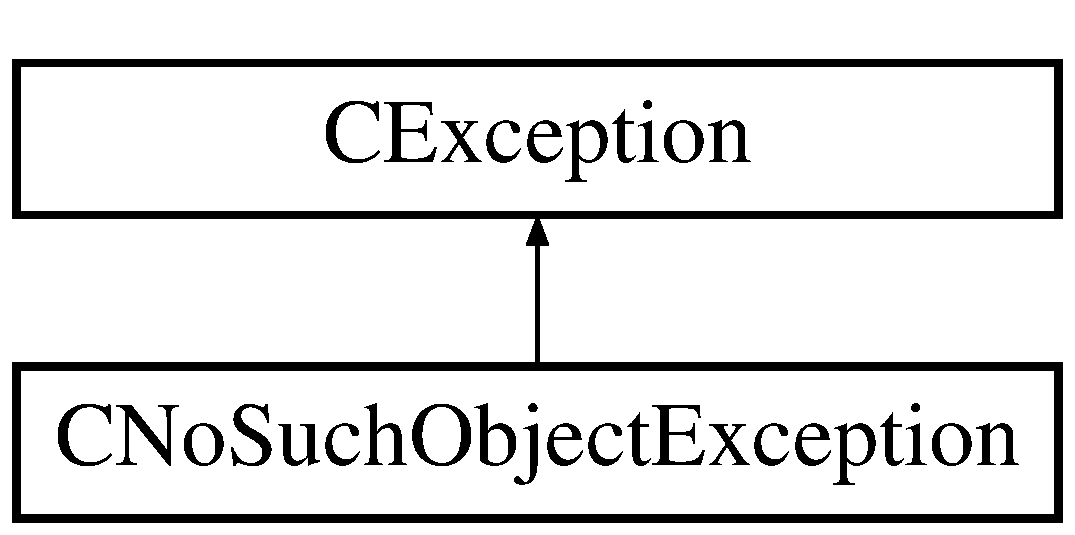
\includegraphics[height=2cm]{classCNoSuchObjectException}
\end{center}
\end{figure}
\subsection*{Public Methods}
\begin{CompactItemize}
\item 
{\bf CNo\-Such\-Object\-Exception} (const char $\ast$p\-Doing, const char $\ast$p\-Name)
\item 
{\bf CNo\-Such\-Object\-Exception} (const char $\ast$p\-Doing, const string \&r\-Name)
\item 
{\bf CNo\-Such\-Object\-Exception} (const string \&r\-Doing, const char $\ast$p\-Name)
\item 
{\bf CNo\-Such\-Object\-Exception} (const string \&r\-Doing, const string \&r\-Name)
\item 
virtual {\bf $\sim$CNo\-Such\-Object\-Exception} ()
\item 
{\bf CNo\-Such\-Object\-Exception} (const CNo\-Such\-Object\-Exception \&a\-CNo\-Such\-Object\-Exception)
\item 
CNo\-Such\-Object\-Exception {\bf operator=} (const CNo\-Such\-Object\-Exception \&a\-CNo\-Such\-Object\-Exception)
\item 
int {\bf operator==} (const CNo\-Such\-Object\-Exception \&a\-CNo\-Such\-Object\-Exception)
\item 
string {\bf get\-Name} () const
\item 
void {\bf set\-Name} (string am\_\-s\-Name)
\item 
virtual const char $\ast$ {\bf Reason\-Text} () const
\end{CompactItemize}
\subsection*{Protected Methods}
\begin{CompactItemize}
\item 
void {\bf Update\-Reason\-Text} ()
\end{CompactItemize}
\subsection*{Private Attributes}
\begin{CompactItemize}
\item 
string {\bf m\_\-s\-Name}
\item 
string {\bf m\_\-s\-Reason\-Text}
\end{CompactItemize}


\subsection{Constructor \& Destructor Documentation}
\index{CNoSuchObjectException@{CNo\-Such\-Object\-Exception}!CNoSuchObjectException@{CNoSuchObjectException}}
\index{CNoSuchObjectException@{CNoSuchObjectException}!CNoSuchObjectException@{CNo\-Such\-Object\-Exception}}
\subsubsection{\setlength{\rightskip}{0pt plus 5cm}CNo\-Such\-Object\-Exception::CNo\-Such\-Object\-Exception (const char $\ast$ {\em p\-Doing}, const char $\ast$ {\em p\-Name})\hspace{0.3cm}{\tt  [inline]}}\label{classCNoSuchObjectException_a0}




Definition at line 299 of file CNo\-Such\-Object\-Exception.h.

References m\_\-s\-Name, and Update\-Reason\-Text().\index{CNoSuchObjectException@{CNo\-Such\-Object\-Exception}!CNoSuchObjectException@{CNoSuchObjectException}}
\index{CNoSuchObjectException@{CNoSuchObjectException}!CNoSuchObjectException@{CNo\-Such\-Object\-Exception}}
\subsubsection{\setlength{\rightskip}{0pt plus 5cm}CNo\-Such\-Object\-Exception::CNo\-Such\-Object\-Exception (const char $\ast$ {\em p\-Doing}, const string \& {\em r\-Name})\hspace{0.3cm}{\tt  [inline]}}\label{classCNoSuchObjectException_a1}




Definition at line 304 of file CNo\-Such\-Object\-Exception.h.

References m\_\-s\-Name, and Update\-Reason\-Text().\index{CNoSuchObjectException@{CNo\-Such\-Object\-Exception}!CNoSuchObjectException@{CNoSuchObjectException}}
\index{CNoSuchObjectException@{CNoSuchObjectException}!CNoSuchObjectException@{CNo\-Such\-Object\-Exception}}
\subsubsection{\setlength{\rightskip}{0pt plus 5cm}CNo\-Such\-Object\-Exception::CNo\-Such\-Object\-Exception (const string \& {\em r\-Doing}, const char $\ast$ {\em p\-Name})\hspace{0.3cm}{\tt  [inline]}}\label{classCNoSuchObjectException_a2}




Definition at line 309 of file CNo\-Such\-Object\-Exception.h.

References m\_\-s\-Name, and Update\-Reason\-Text().\index{CNoSuchObjectException@{CNo\-Such\-Object\-Exception}!CNoSuchObjectException@{CNoSuchObjectException}}
\index{CNoSuchObjectException@{CNoSuchObjectException}!CNoSuchObjectException@{CNo\-Such\-Object\-Exception}}
\subsubsection{\setlength{\rightskip}{0pt plus 5cm}CNo\-Such\-Object\-Exception::CNo\-Such\-Object\-Exception (const string \& {\em r\-Doing}, const string \& {\em r\-Name})\hspace{0.3cm}{\tt  [inline]}}\label{classCNoSuchObjectException_a3}




Definition at line 314 of file CNo\-Such\-Object\-Exception.h.

References m\_\-s\-Name, and Update\-Reason\-Text().\index{CNoSuchObjectException@{CNo\-Such\-Object\-Exception}!~CNoSuchObjectException@{$\sim$CNoSuchObjectException}}
\index{~CNoSuchObjectException@{$\sim$CNoSuchObjectException}!CNoSuchObjectException@{CNo\-Such\-Object\-Exception}}
\subsubsection{\setlength{\rightskip}{0pt plus 5cm}virtual CNo\-Such\-Object\-Exception::$\sim$CNo\-Such\-Object\-Exception ()\hspace{0.3cm}{\tt  [inline, virtual]}}\label{classCNoSuchObjectException_a4}




Definition at line 319 of file CNo\-Such\-Object\-Exception.h.\index{CNoSuchObjectException@{CNo\-Such\-Object\-Exception}!CNoSuchObjectException@{CNoSuchObjectException}}
\index{CNoSuchObjectException@{CNoSuchObjectException}!CNoSuchObjectException@{CNo\-Such\-Object\-Exception}}
\subsubsection{\setlength{\rightskip}{0pt plus 5cm}CNo\-Such\-Object\-Exception::CNo\-Such\-Object\-Exception (const CNo\-Such\-Object\-Exception \& {\em a\-CNo\-Such\-Object\-Exception})\hspace{0.3cm}{\tt  [inline]}}\label{classCNoSuchObjectException_a5}




Definition at line 323 of file CNo\-Such\-Object\-Exception.h.

References m\_\-s\-Name, and Update\-Reason\-Text().

\subsection{Member Function Documentation}
\index{CNoSuchObjectException@{CNo\-Such\-Object\-Exception}!getName@{getName}}
\index{getName@{getName}!CNoSuchObjectException@{CNo\-Such\-Object\-Exception}}
\subsubsection{\setlength{\rightskip}{0pt plus 5cm}string CNo\-Such\-Object\-Exception::get\-Name () const\hspace{0.3cm}{\tt  [inline]}}\label{classCNoSuchObjectException_a8}




Definition at line 353 of file CNo\-Such\-Object\-Exception.h.

References m\_\-s\-Name.\index{CNoSuchObjectException@{CNo\-Such\-Object\-Exception}!operator=@{operator=}}
\index{operator=@{operator=}!CNoSuchObjectException@{CNo\-Such\-Object\-Exception}}
\subsubsection{\setlength{\rightskip}{0pt plus 5cm}CNo\-Such\-Object\-Exception CNo\-Such\-Object\-Exception::operator= (const CNo\-Such\-Object\-Exception \& {\em a\-CNo\-Such\-Object\-Exception})\hspace{0.3cm}{\tt  [inline]}}\label{classCNoSuchObjectException_a6}




Definition at line 333 of file CNo\-Such\-Object\-Exception.h.

References m\_\-s\-Name, CException::operator=(), and Update\-Reason\-Text().\index{CNoSuchObjectException@{CNo\-Such\-Object\-Exception}!operator==@{operator==}}
\index{operator==@{operator==}!CNoSuchObjectException@{CNo\-Such\-Object\-Exception}}
\subsubsection{\setlength{\rightskip}{0pt plus 5cm}int CNo\-Such\-Object\-Exception::operator== (const CNo\-Such\-Object\-Exception \& {\em a\-CNo\-Such\-Object\-Exception})\hspace{0.3cm}{\tt  [inline]}}\label{classCNoSuchObjectException_a7}




Definition at line 344 of file CNo\-Such\-Object\-Exception.h.

References m\_\-s\-Name, and CException::operator==().\index{CNoSuchObjectException@{CNo\-Such\-Object\-Exception}!ReasonText@{ReasonText}}
\index{ReasonText@{ReasonText}!CNoSuchObjectException@{CNo\-Such\-Object\-Exception}}
\subsubsection{\setlength{\rightskip}{0pt plus 5cm}const char $\ast$ CNo\-Such\-Object\-Exception::Reason\-Text () const\hspace{0.3cm}{\tt  [virtual]}}\label{classCNoSuchObjectException_a10}


Returns a const pointer to text which describes the reason the exception was thrown. This is exception type specific. The default action returns a pointer to the constant string: \char`\"{}Unspecified Exception\char`\"{} 

Reimplemented from {\bf CException} {\rm (p.\,\pageref{classCException_a8})}.

Definition at line 284 of file CNo\-Such\-Object\-Exception.cpp.

References m\_\-s\-Reason\-Text.\index{CNoSuchObjectException@{CNo\-Such\-Object\-Exception}!setName@{setName}}
\index{setName@{setName}!CNoSuchObjectException@{CNo\-Such\-Object\-Exception}}
\subsubsection{\setlength{\rightskip}{0pt plus 5cm}void CNo\-Such\-Object\-Exception::set\-Name (string {\em am\_\-s\-Name})\hspace{0.3cm}{\tt  [inline]}}\label{classCNoSuchObjectException_a9}




Definition at line 359 of file CNo\-Such\-Object\-Exception.h.

References m\_\-s\-Name.\index{CNoSuchObjectException@{CNo\-Such\-Object\-Exception}!UpdateReasonText@{UpdateReasonText}}
\index{UpdateReasonText@{UpdateReasonText}!CNoSuchObjectException@{CNo\-Such\-Object\-Exception}}
\subsubsection{\setlength{\rightskip}{0pt plus 5cm}void CNo\-Such\-Object\-Exception::Update\-Reason\-Text ()\hspace{0.3cm}{\tt  [protected]}}\label{classCNoSuchObjectException_b0}




Definition at line 290 of file CNo\-Such\-Object\-Exception.cpp.

References m\_\-s\-Name, and m\_\-s\-Reason\-Text.

Referenced by CNo\-Such\-Object\-Exception(), and operator=().

\subsection{Member Data Documentation}
\index{CNoSuchObjectException@{CNo\-Such\-Object\-Exception}!m_sName@{m\_\-sName}}
\index{m_sName@{m\_\-sName}!CNoSuchObjectException@{CNo\-Such\-Object\-Exception}}
\subsubsection{\setlength{\rightskip}{0pt plus 5cm}string CNo\-Such\-Object\-Exception::m\_\-s\-Name\hspace{0.3cm}{\tt  [private]}}\label{classCNoSuchObjectException_o0}




Definition at line 295 of file CNo\-Such\-Object\-Exception.h.

Referenced by CNo\-Such\-Object\-Exception(), get\-Name(), operator=(), operator==(), set\-Name(), and Update\-Reason\-Text().\index{CNoSuchObjectException@{CNo\-Such\-Object\-Exception}!m_sReasonText@{m\_\-sReasonText}}
\index{m_sReasonText@{m\_\-sReasonText}!CNoSuchObjectException@{CNo\-Such\-Object\-Exception}}
\subsubsection{\setlength{\rightskip}{0pt plus 5cm}string CNo\-Such\-Object\-Exception::m\_\-s\-Reason\-Text\hspace{0.3cm}{\tt  [private]}}\label{classCNoSuchObjectException_o1}




Definition at line 296 of file CNo\-Such\-Object\-Exception.h.

Referenced by Reason\-Text(), and Update\-Reason\-Text().

The documentation for this class was generated from the following files:\begin{CompactItemize}
\item 
{\bf CNo\-Such\-Object\-Exception.h}\item 
{\bf CNo\-Such\-Object\-Exception.cpp}\end{CompactItemize}

\section{CObject\-Registry  Class Reference}
\label{classCObjectRegistry}\index{CObjectRegistry@{CObject\-Registry}}
{\tt \#include $<$CObject\-Registry.h$>$}

Inheritance diagram for CObject\-Registry::\begin{figure}[H]
\begin{center}
\leavevmode
\includegraphics[height=2cm]{classCObjectRegistry}
\end{center}
\end{figure}
\subsection*{Public Methods}
\begin{CompactItemize}
\item 
{\bf CObject\-Registry} (string am\_\-s\-Name)
\item 
virtual {\bf $\sim$CObject\-Registry} ()
\item 
map$<$ string, {\bf CNamed\-Object} $\ast$ $>$ {\bf get\-Objects} () const
\item 
void {\bf Add} ({\bf CNamed\-Object} \&r\-Object)
\item 
void {\bf Remove} (const string \&r\-Name)
\item 
void {\bf Remove} (const {\bf CNamed\-Object} \&r\-Object)
\item 
const {\bf Object\-Iterator} {\bf Find} (const string \&r\-Object\-Name) const
\item 
{\bf Object\-Iterator} {\bf begin} ()
\item 
{\bf Object\-Iterator} {\bf end} ()
\item 
virtual string {\bf Describe\-Self} ()
\end{CompactItemize}
\subsection*{Protected Methods}
\begin{CompactItemize}
\item 
void {\bf set\-Objects} (map$<$ string, {\bf CNamed\-Object} $\ast$ $>$ am\_\-Objects)
\end{CompactItemize}
\subsection*{Private Attributes}
\begin{CompactItemize}
\item 
map$<$ string, {\bf CNamed\-Object} $\ast$ $>$ {\bf m\_\-Objects}
\end{CompactItemize}


\subsection{Detailed Description}
Implements a registry of named objects.  Registries allow you to determine which instances of particular types of objects exist. Typically a programmer wanting to  allow this level of introspection will subclass a class hierarchy from {\bf CRegistered\-Object} {\rm (p.\,\pageref{classCRegisteredObject})} such that the constructor of each class will register that class. One can then programmatically search for named instances of a class as well as iterate through the registry to determine which instances exist. 



Definition at line 321 of file CObject\-Registry.h.

\subsection{Constructor \& Destructor Documentation}
\index{CObjectRegistry@{CObject\-Registry}!CObjectRegistry@{CObjectRegistry}}
\index{CObjectRegistry@{CObjectRegistry}!CObjectRegistry@{CObject\-Registry}}
\subsubsection{\setlength{\rightskip}{0pt plus 5cm}CObject\-Registry::CObject\-Registry (string {\em am\_\-s\-Name})\hspace{0.3cm}{\tt  [inline]}}\label{classCObjectRegistry_a0}


Map containing the name key and a pointer to the object. 

Definition at line 329 of file CObject\-Registry.h.

References CNamed\-Object::Append\-Class\-Info().\index{CObjectRegistry@{CObject\-Registry}!~CObjectRegistry@{$\sim$CObjectRegistry}}
\index{~CObjectRegistry@{$\sim$CObjectRegistry}!CObjectRegistry@{CObject\-Registry}}
\subsubsection{\setlength{\rightskip}{0pt plus 5cm}virtual CObject\-Registry::$\sim$CObject\-Registry ()\hspace{0.3cm}{\tt  [inline, virtual]}}\label{classCObjectRegistry_a1}




Definition at line 334 of file CObject\-Registry.h.

\subsection{Member Function Documentation}
\index{CObjectRegistry@{CObject\-Registry}!Add@{Add}}
\index{Add@{Add}!CObjectRegistry@{CObject\-Registry}}
\subsubsection{\setlength{\rightskip}{0pt plus 5cm}void CObject\-Registry::Add ({\bf CNamed\-Object} \& {\em r\-Object})}\label{classCObjectRegistry_a3}


Adds an object to the object registry.  The name of the object is gotten from the object itself.\begin{Desc}
\item[Parameters: ]\par
\begin{description}
\item[{\em 
r\-Object}]The object to add to the registry. \end{description}
\end{Desc}


Definition at line 310 of file CObject\-Registry.cpp.

References CNamed\-Object::get\-Name(), and m\_\-Objects.\index{CObjectRegistry@{CObject\-Registry}!begin@{begin}}
\index{begin@{begin}!CObjectRegistry@{CObject\-Registry}}
\subsubsection{\setlength{\rightskip}{0pt plus 5cm}{\bf Object\-Iterator} CObject\-Registry::begin ()}\label{classCObjectRegistry_a7}


Returns an iterator which 'points' to the beginning of the  registry of objects. Traversing the registry through this  iterator will visit all objects in name alphabetical order. 

Definition at line 386 of file CObject\-Registry.cpp.

References m\_\-Objects.\index{CObjectRegistry@{CObject\-Registry}!DescribeSelf@{DescribeSelf}}
\index{DescribeSelf@{DescribeSelf}!CObjectRegistry@{CObject\-Registry}}
\subsubsection{\setlength{\rightskip}{0pt plus 5cm}string CObject\-Registry::Describe\-Self ()\hspace{0.3cm}{\tt  [virtual]}}\label{classCObjectRegistry_a9}


Returns a string which describes the registry The description includes the name and class path of the registry, and the name and class path of all objects contained in the registry. 

Reimplemented from {\bf CNamed\-Object} {\rm (p.\,\pageref{classCNamedObject_a8})}.

Definition at line 409 of file CObject\-Registry.cpp.

References CNamed\-Object::Describe\-Self(), m\_\-Objects, and Object\-Iterator.\index{CObjectRegistry@{CObject\-Registry}!end@{end}}
\index{end@{end}!CObjectRegistry@{CObject\-Registry}}
\subsubsection{\setlength{\rightskip}{0pt plus 5cm}{\bf Object\-Iterator} CObject\-Registry::end ()}\label{classCObjectRegistry_a8}


Returns an iterator which 'points' off the end of the registry of objects. Provided to allow clients to know when to terminate iteration through the registry. 

Definition at line 397 of file CObject\-Registry.cpp.

References m\_\-Objects.\index{CObjectRegistry@{CObject\-Registry}!Find@{Find}}
\index{Find@{Find}!CObjectRegistry@{CObject\-Registry}}
\subsubsection{\setlength{\rightskip}{0pt plus 5cm}const {\bf Object\-Iterator} CObject\-Registry::Find (const string \& {\em r\-Object\-Name}) const}\label{classCObjectRegistry_a6}


Searches the registry for an object name. If the object exists in the registry, an Object\-Iterator pointing to the object is returned. If it does not exist, a {\bf CNo\-Such\-Object\-Exception} {\rm (p.\,\pageref{classCNoSuchObjectException})} is thrown.\begin{Desc}
\item[Parameters: ]\par
\begin{description}
\item[{\em 
r\-Object\-Name}]The name of the object to find. \end{description}
\end{Desc}


Definition at line 368 of file CObject\-Registry.cpp.

References m\_\-Objects, and Object\-Iterator.\index{CObjectRegistry@{CObject\-Registry}!getObjects@{getObjects}}
\index{getObjects@{getObjects}!CObjectRegistry@{CObject\-Registry}}
\subsubsection{\setlength{\rightskip}{0pt plus 5cm}map$<$string, {\bf CNamed\-Object}$\ast$$>$ CObject\-Registry::get\-Objects () const\hspace{0.3cm}{\tt  [inline]}}\label{classCObjectRegistry_a2}




Definition at line 339 of file CObject\-Registry.h.

References m\_\-Objects.\index{CObjectRegistry@{CObject\-Registry}!Remove@{Remove}}
\index{Remove@{Remove}!CObjectRegistry@{CObject\-Registry}}
\subsubsection{\setlength{\rightskip}{0pt plus 5cm}void CObject\-Registry::Remove (const {\bf CNamed\-Object} \& {\em r\-Object})}\label{classCObjectRegistry_a5}


Removes an object from the object registry. The name of the object is obtained from the object itself. If the name does not exist in the registry, a  {\bf CNo\-Such\-Object\-Exception} {\rm (p.\,\pageref{classCNoSuchObjectException})} is thrown.\begin{Desc}
\item[Parameters: ]\par
\begin{description}
\item[{\em 
r\-Object}]The object to be removed from the registry. \end{description}
\end{Desc}


Definition at line 350 of file CObject\-Registry.cpp.

References CNamed\-Object::get\-Name(), and m\_\-Objects.\index{CObjectRegistry@{CObject\-Registry}!Remove@{Remove}}
\index{Remove@{Remove}!CObjectRegistry@{CObject\-Registry}}
\subsubsection{\setlength{\rightskip}{0pt plus 5cm}void CObject\-Registry::Remove (const string \& {\em r\-Name})}\label{classCObjectRegistry_a4}


Removes an object from the object registry. The name of the object is inserted into the registry. If the name does not exists, a {\bf CNo\-Such\-Object\-Exception} {\rm (p.\,\pageref{classCNoSuchObjectException})} is  thrown.\begin{Desc}
\item[Parameters: ]\par
\begin{description}
\item[{\em 
r\-Name}]The name of the object to remove from the registry. \end{description}
\end{Desc}


Definition at line 332 of file CObject\-Registry.cpp.

References m\_\-Objects.\index{CObjectRegistry@{CObject\-Registry}!setObjects@{setObjects}}
\index{setObjects@{setObjects}!CObjectRegistry@{CObject\-Registry}}
\subsubsection{\setlength{\rightskip}{0pt plus 5cm}void CObject\-Registry::set\-Objects (map$<$ string, {\bf CNamed\-Object} $\ast$ $>$ {\em am\_\-Objects})\hspace{0.3cm}{\tt  [inline, protected]}}\label{classCObjectRegistry_b0}




Definition at line 347 of file CObject\-Registry.h.

References m\_\-Objects.

\subsection{Member Data Documentation}
\index{CObjectRegistry@{CObject\-Registry}!m_Objects@{m\_\-Objects}}
\index{m_Objects@{m\_\-Objects}!CObjectRegistry@{CObject\-Registry}}
\subsubsection{\setlength{\rightskip}{0pt plus 5cm}map$<$string, {\bf CNamed\-Object}$\ast$$>$ CObject\-Registry::m\_\-Objects\hspace{0.3cm}{\tt  [private]}}\label{classCObjectRegistry_o0}




Definition at line 323 of file CObject\-Registry.h.

Referenced by Add(), begin(), Describe\-Self(), end(), Find(), get\-Objects(), Remove(), and set\-Objects().

The documentation for this class was generated from the following files:\begin{CompactItemize}
\item 
{\bf CObject\-Registry.h}\item 
{\bf CObject\-Registry.cpp}\end{CompactItemize}

\section{CPointer\-Predicate$<$ T $>$  Class Template Reference}
\label{classCPointerPredicate}\index{CPointerPredicate@{CPointer\-Predicate}}
{\tt \#include $<$CPointer\-Predicate.h$>$}

Inheritance diagram for CPointer\-Predicate$<$ T $>$::\begin{figure}[H]
\begin{center}
\leavevmode
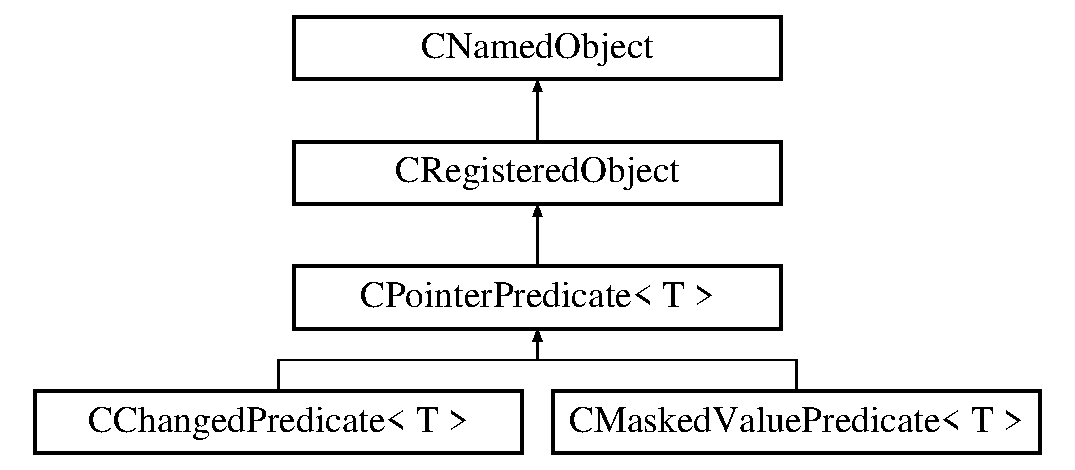
\includegraphics[height=4cm]{classCPointerPredicate}
\end{center}
\end{figure}
\subsection*{Public Methods}
\begin{CompactItemize}
\item 
{\bf CPointer\-Predicate} ()
\item 
{\bf CPointer\-Predicate} (const string \&r\-Name)
\item 
{\bf CPointer\-Predicate} (const char $\ast$p\-Name)
\item 
{\bf $\sim$CPointer\-Predicate} ()
\item 
int {\bf operator==} (const CPointer\-Predicate$<$ T $>$ \&a\-CPointer\-Predicate) const
\item 
virtual bool {\bf operator()} (T n\-Value)=0
\item 
virtual string {\bf Describe\-Self} ()=0
\end{CompactItemize}
\subsection*{Static Protected Methods}
\begin{CompactItemize}
\item 
string {\bf Get\-Auto\-Name} (const string \&r\-Base\-Name)
\end{CompactItemize}
\subsection*{Private Methods}
\begin{CompactItemize}
\item 
{\bf CPointer\-Predicate} (const CPointer\-Predicate$<$ T $>$ \&a\-CPointer\-Predicate)
\item 
CPointer\-Predicate$<$ T $>$ {\bf operator=} (const CPointer\-Predicate$<$ T $>$ \&a\-CPointer\-Predicate)
\end{CompactItemize}
\subsection*{Static Private Attributes}
\begin{CompactItemize}
\item 
unsigned int {\bf m\_\-n\-Auto\-Index} = 0
\begin{CompactList}\small\item\em Used to name autonamed objects.\item\end{CompactList}\end{CompactItemize}
\subsubsection*{template$<$typename T$>$ class CPointer\-Predicate$<$ T $>$}



\subsection{Constructor \& Destructor Documentation}
\index{CPointerPredicate@{CPointer\-Predicate}!CPointerPredicate@{CPointerPredicate}}
\index{CPointerPredicate@{CPointerPredicate}!CPointerPredicate@{CPointer\-Predicate}}
\subsubsection{\setlength{\rightskip}{0pt plus 5cm}template$<$typename T$>$ CPointer\-Predicate$<$ T $>$::CPointer\-Predicate ()\hspace{0.3cm}{\tt  [inline]}}\label{classCPointerPredicate_a0}


Used to name predicate objects \index{CPointerPredicate@{CPointer\-Predicate}!CPointerPredicate@{CPointerPredicate}}
\index{CPointerPredicate@{CPointerPredicate}!CPointerPredicate@{CPointer\-Predicate}}
\subsubsection{\setlength{\rightskip}{0pt plus 5cm}template$<$typename T$>$ CPointer\-Predicate$<$ T $>$::CPointer\-Predicate (const string \& {\em r\-Name})\hspace{0.3cm}{\tt  [inline]}}\label{classCPointerPredicate_a1}


\index{CPointerPredicate@{CPointer\-Predicate}!CPointerPredicate@{CPointerPredicate}}
\index{CPointerPredicate@{CPointerPredicate}!CPointerPredicate@{CPointer\-Predicate}}
\subsubsection{\setlength{\rightskip}{0pt plus 5cm}template$<$typename T$>$ CPointer\-Predicate$<$ T $>$::CPointer\-Predicate (const char $\ast$ {\em p\-Name})\hspace{0.3cm}{\tt  [inline]}}\label{classCPointerPredicate_a2}


\index{CPointerPredicate@{CPointer\-Predicate}!~CPointerPredicate@{$\sim$CPointerPredicate}}
\index{~CPointerPredicate@{$\sim$CPointerPredicate}!CPointerPredicate@{CPointer\-Predicate}}
\subsubsection{\setlength{\rightskip}{0pt plus 5cm}template$<$typename T$>$ CPointer\-Predicate$<$ T $>$::$\sim$CPointer\-Predicate ()\hspace{0.3cm}{\tt  [inline]}}\label{classCPointerPredicate_a3}


\index{CPointerPredicate@{CPointer\-Predicate}!CPointerPredicate@{CPointerPredicate}}
\index{CPointerPredicate@{CPointerPredicate}!CPointerPredicate@{CPointer\-Predicate}}
\subsubsection{\setlength{\rightskip}{0pt plus 5cm}template$<$typename T$>$ CPointer\-Predicate$<$ T $>$::CPointer\-Predicate (const CPointer\-Predicate$<$ T $>$ \& {\em a\-CPointer\-Predicate})\hspace{0.3cm}{\tt  [private]}}\label{classCPointerPredicate_c0}




\subsection{Member Function Documentation}
\index{CPointerPredicate@{CPointer\-Predicate}!DescribeSelf@{DescribeSelf}}
\index{DescribeSelf@{DescribeSelf}!CPointerPredicate@{CPointer\-Predicate}}
\subsubsection{\setlength{\rightskip}{0pt plus 5cm}template$<$typename T$>$ virtual string CPointer\-Predicate$<$ T $>$::Describe\-Self ()\hspace{0.3cm}{\tt  [pure virtual]}}\label{classCPointerPredicate_a6}


Describes the named object. The information given is the object type given by m\_\-s\-Class\-Path, and the object name. 

Reimplemented from {\bf CNamed\-Object} {\rm (p.\,\pageref{classCNamedObject_a8})}.

Implemented in {\bf CChanged\-Predicate$<$ T $>$} {\rm (p.\,\pageref{classCChangedPredicate_a7})}, and {\bf CMasked\-Value\-Predicate$<$ T $>$} {\rm (p.\,\pageref{classCMaskedValuePredicate_a8})}.\index{CPointerPredicate@{CPointer\-Predicate}!GetAutoName@{GetAutoName}}
\index{GetAutoName@{GetAutoName}!CPointerPredicate@{CPointer\-Predicate}}
\subsubsection{\setlength{\rightskip}{0pt plus 5cm}template$<$typename T$>$ string CPointer\-Predicate$<$ T $>$::Get\-Auto\-Name (const string \& {\em r\-Base\-Name})\hspace{0.3cm}{\tt  [static, protected]}}\label{classCPointerPredicate_e0}


$\backslash$function string {\bf CPointer\-Predicate::Get\-Auto\-Name}(const string\& r\-Base\-Name) {\rm (p.\,\pageref{classCPointerPredicate_e0})} Automatically names an object given its base class(es)\begin{Desc}
\item[Parameters: ]\par
\begin{description}
\item[{\em 
const}]string\& r\-Base\-Name The base name of the object being named \end{description}
\end{Desc}


Reimplemented from {\bf CNamed\-Object} {\rm (p.\,\pageref{classCNamedObject_e0})}.

Definition at line 296 of file CPointer\-Predicate.cpp.

References CPointer\-Predicate$<$ T $>$::m\_\-n\-Auto\-Index.\index{CPointerPredicate@{CPointer\-Predicate}!operator()@{operator()}}
\index{operator()@{operator()}!CPointerPredicate@{CPointer\-Predicate}}
\subsubsection{\setlength{\rightskip}{0pt plus 5cm}template$<$typename T$>$ virtual bool CPointer\-Predicate$<$ T $>$::operator() (T {\em n\-Value})\hspace{0.3cm}{\tt  [pure virtual]}}\label{classCPointerPredicate_a5}




Implemented in {\bf CChanged\-Predicate$<$ T $>$} {\rm (p.\,\pageref{classCChangedPredicate_a6})}, and {\bf CMasked\-Value\-Predicate$<$ T $>$} {\rm (p.\,\pageref{classCMaskedValuePredicate_a7})}.\index{CPointerPredicate@{CPointer\-Predicate}!operator=@{operator=}}
\index{operator=@{operator=}!CPointerPredicate@{CPointer\-Predicate}}
\subsubsection{\setlength{\rightskip}{0pt plus 5cm}template$<$typename T$>$ CPointer\-Predicate$<$T$>$ CPointer\-Predicate$<$ T $>$::operator= (const CPointer\-Predicate$<$ T $>$ \& {\em a\-CPointer\-Predicate})\hspace{0.3cm}{\tt  [private]}}\label{classCPointerPredicate_c1}


\index{CPointerPredicate@{CPointer\-Predicate}!operator==@{operator==}}
\index{operator==@{operator==}!CPointerPredicate@{CPointer\-Predicate}}
\subsubsection{\setlength{\rightskip}{0pt plus 5cm}template$<$typename T$>$ int CPointer\-Predicate$<$ T $>$::operator== (const CPointer\-Predicate$<$ T $>$ \& {\em a\-CPointer\-Predicate}) const\hspace{0.3cm}{\tt  [inline]}}\label{classCPointerPredicate_a4}




Definition at line 335 of file CPointer\-Predicate.h.

References CRegistered\-Object::operator==().

Referenced by CMasked\-Value\-Predicate$<$ T $>$::operator==(), and CChanged\-Predicate$<$ T $>$::operator==().

\subsection{Member Data Documentation}
\index{CPointerPredicate@{CPointer\-Predicate}!m_nAutoIndex@{m\_\-nAutoIndex}}
\index{m_nAutoIndex@{m\_\-nAutoIndex}!CPointerPredicate@{CPointer\-Predicate}}
\subsubsection{\setlength{\rightskip}{0pt plus 5cm}template$<$typename T$>$ unsigned int CPointer\-Predicate$<$ T $>$::m\_\-n\-Auto\-Index = 0\hspace{0.3cm}{\tt  [static, private]}}\label{classCPointerPredicate_r0}


Used to name autonamed objects.

Named\-Object.cpp Base class for all objects in the event management system.

Author: Jason Venema NSCL Michigan State University East Lansing, MI 48824-1321 mailto:{\tt venemaja@msu.edu} 

Reimplemented from {\bf CNamed\-Object} {\rm (p.\,\pageref{classCNamedObject_r0})}.

Definition at line 283 of file CPointer\-Predicate.cpp.

Referenced by CPointer\-Predicate$<$ T $>$::Get\-Auto\-Name().

The documentation for this class was generated from the following files:\begin{CompactItemize}
\item 
{\bf CPointer\-Predicate.h}\item 
{\bf CPointer\-Predicate.cpp}\end{CompactItemize}

\section{CRange\-Error  Class Reference}
\label{classCRangeError}\index{CRangeError@{CRange\-Error}}
{\tt \#include $<$CRange\-Error.h$>$}

Inheritance diagram for CRange\-Error::\begin{figure}[H]
\begin{center}
\leavevmode
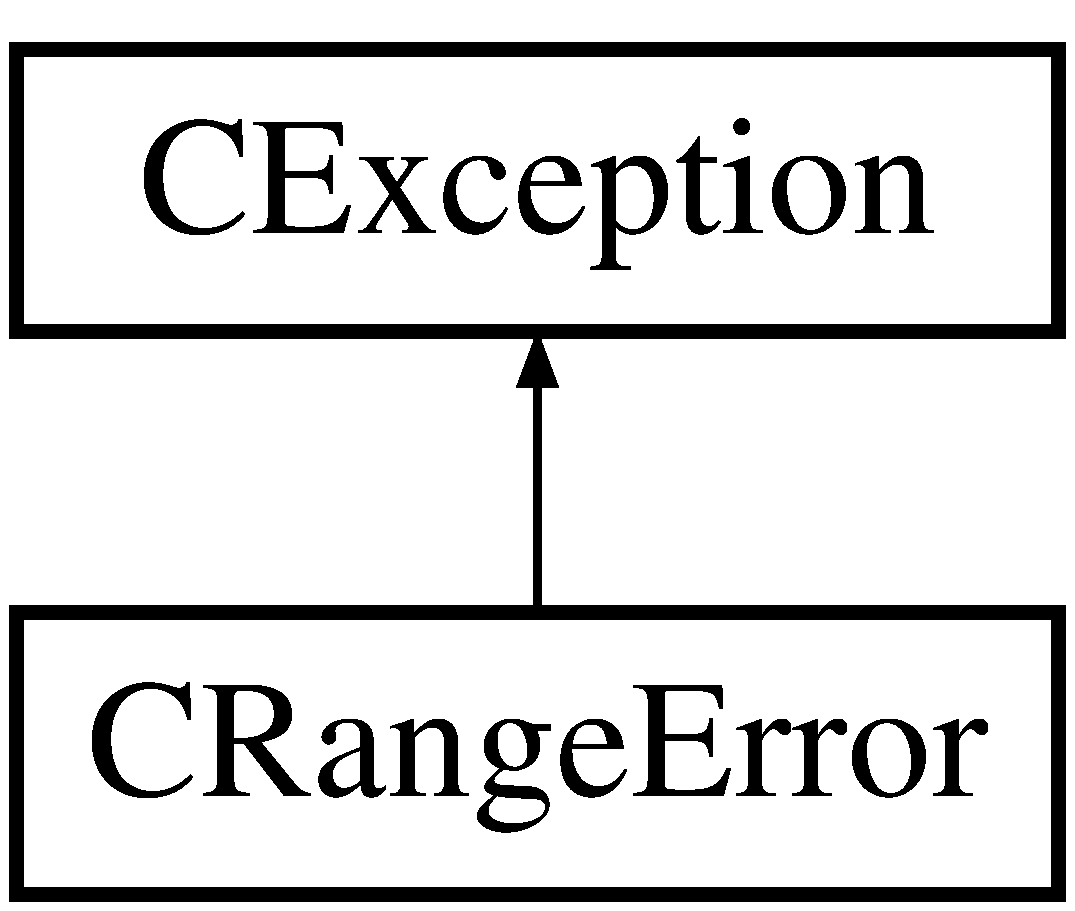
\includegraphics[height=2cm]{classCRangeError}
\end{center}
\end{figure}
\subsection*{Public Types}
\begin{CompactItemize}
\item 
enum \{ {\bf kn\-Too\-Low}, 
{\bf kn\-Too\-High}
 \}
\end{CompactItemize}
\subsection*{Public Methods}
\begin{CompactItemize}
\item 
{\bf CRange\-Error} ({\bf Int\_\-t} n\-Low, {\bf Int\_\-t} n\-High, {\bf Int\_\-t} n\-Requested, const char $\ast$p\-Doing)
\item 
{\bf CRange\-Error} ({\bf Int\_\-t} n\-Low, {\bf Int\_\-t} n\-High, {\bf Int\_\-t} n\-Requested, const string \&r\-Doing)
\item 
virtual {\bf $\sim$CRange\-Error} ()
\item 
{\bf CRange\-Error} (const CRange\-Error \&a\-CRange\-Error)
\item 
CRange\-Error {\bf operator=} (const CRange\-Error \&a\-CRange\-Error)
\item 
int {\bf operator==} (const CRange\-Error \&a\-CRange\-Error)
\item 
{\bf Int\_\-t} {\bf get\-Low} () const
\item 
{\bf Int\_\-t} {\bf get\-High} () const
\item 
{\bf Int\_\-t} {\bf get\-Requested} () const
\item 
virtual const char $\ast$ {\bf Reason\-Text} () const
\item 
virtual {\bf Int\_\-t} {\bf Reason\-Code} () const
\end{CompactItemize}
\subsection*{Protected Methods}
\begin{CompactItemize}
\item 
void {\bf set\-Low} ({\bf Int\_\-t} am\_\-n\-Low)
\item 
void {\bf set\-High} ({\bf Int\_\-t} am\_\-n\-High)
\item 
void {\bf set\-Requested} ({\bf Int\_\-t} am\_\-n\-Requested)
\item 
void {\bf Update\-Reason} ()
\end{CompactItemize}
\subsection*{Private Attributes}
\begin{CompactItemize}
\item 
{\bf Int\_\-t} {\bf m\_\-n\-Low}
\item 
{\bf Int\_\-t} {\bf m\_\-n\-High}
\item 
{\bf Int\_\-t} {\bf m\_\-n\-Requested}
\item 
string {\bf m\_\-Reason\-Text}
\end{CompactItemize}


\subsection{Member Enumeration Documentation}
\subsubsection{\setlength{\rightskip}{0pt plus 5cm}anonymous enum}\label{classCRangeError_s2}


\begin{Desc}
\item[Enumeration values:]\par
\begin{description}
\index{knTooLow@{knTooLow}!CRangeError@{CRange\-Error}}\index{CRangeError@{CRangeError}!knTooLow@{kn\-Too\-Low}}\item[{\em 
{\em kn\-Too\-Low}\label{classCRangeError_s2s0}
}]\index{knTooHigh@{knTooHigh}!CRangeError@{CRange\-Error}}\index{CRangeError@{CRangeError}!knTooHigh@{kn\-Too\-High}}\item[{\em 
{\em kn\-Too\-High}\label{classCRangeError_s2s1}
}]\end{description}
\end{Desc}



Definition at line 315 of file CRange\-Error.h.

\subsection{Constructor \& Destructor Documentation}
\index{CRangeError@{CRange\-Error}!CRangeError@{CRangeError}}
\index{CRangeError@{CRangeError}!CRangeError@{CRange\-Error}}
\subsubsection{\setlength{\rightskip}{0pt plus 5cm}CRange\-Error::CRange\-Error ({\bf Int\_\-t} {\em n\-Low}, {\bf Int\_\-t} {\em n\-High}, {\bf Int\_\-t} {\em n\-Requested}, const char $\ast$ {\em p\-Doing})\hspace{0.3cm}{\tt  [inline]}}\label{classCRangeError_a0}




Definition at line 321 of file CRange\-Error.h.

References Int\_\-t, m\_\-n\-High, m\_\-n\-Low, m\_\-n\-Requested, and Update\-Reason().\index{CRangeError@{CRange\-Error}!CRangeError@{CRangeError}}
\index{CRangeError@{CRangeError}!CRangeError@{CRange\-Error}}
\subsubsection{\setlength{\rightskip}{0pt plus 5cm}CRange\-Error::CRange\-Error ({\bf Int\_\-t} {\em n\-Low}, {\bf Int\_\-t} {\em n\-High}, {\bf Int\_\-t} {\em n\-Requested}, const string \& {\em r\-Doing})\hspace{0.3cm}{\tt  [inline]}}\label{classCRangeError_a1}




Definition at line 328 of file CRange\-Error.h.

References Int\_\-t, m\_\-n\-High, m\_\-n\-Low, m\_\-n\-Requested, and Update\-Reason().\index{CRangeError@{CRange\-Error}!~CRangeError@{$\sim$CRangeError}}
\index{~CRangeError@{$\sim$CRangeError}!CRangeError@{CRange\-Error}}
\subsubsection{\setlength{\rightskip}{0pt plus 5cm}virtual CRange\-Error::$\sim$CRange\-Error ()\hspace{0.3cm}{\tt  [inline, virtual]}}\label{classCRangeError_a2}




Definition at line 335 of file CRange\-Error.h.\index{CRangeError@{CRange\-Error}!CRangeError@{CRangeError}}
\index{CRangeError@{CRangeError}!CRangeError@{CRange\-Error}}
\subsubsection{\setlength{\rightskip}{0pt plus 5cm}CRange\-Error::CRange\-Error (const CRange\-Error \& {\em a\-CRange\-Error})\hspace{0.3cm}{\tt  [inline]}}\label{classCRangeError_a3}




Definition at line 339 of file CRange\-Error.h.

References m\_\-n\-High, m\_\-n\-Low, m\_\-n\-Requested, and Update\-Reason().

\subsection{Member Function Documentation}
\index{CRangeError@{CRange\-Error}!getHigh@{getHigh}}
\index{getHigh@{getHigh}!CRangeError@{CRange\-Error}}
\subsubsection{\setlength{\rightskip}{0pt plus 5cm}{\bf Int\_\-t} CRange\-Error::get\-High () const\hspace{0.3cm}{\tt  [inline]}}\label{classCRangeError_a7}




Definition at line 384 of file CRange\-Error.h.

References Int\_\-t, and m\_\-n\-High.\index{CRangeError@{CRange\-Error}!getLow@{getLow}}
\index{getLow@{getLow}!CRangeError@{CRange\-Error}}
\subsubsection{\setlength{\rightskip}{0pt plus 5cm}{\bf Int\_\-t} CRange\-Error::get\-Low () const\hspace{0.3cm}{\tt  [inline]}}\label{classCRangeError_a6}




Definition at line 380 of file CRange\-Error.h.

References Int\_\-t, and m\_\-n\-Low.\index{CRangeError@{CRange\-Error}!getRequested@{getRequested}}
\index{getRequested@{getRequested}!CRangeError@{CRange\-Error}}
\subsubsection{\setlength{\rightskip}{0pt plus 5cm}{\bf Int\_\-t} CRange\-Error::get\-Requested () const\hspace{0.3cm}{\tt  [inline]}}\label{classCRangeError_a8}




Definition at line 388 of file CRange\-Error.h.

References Int\_\-t, and m\_\-n\-Requested.\index{CRangeError@{CRange\-Error}!operator=@{operator=}}
\index{operator=@{operator=}!CRangeError@{CRange\-Error}}
\subsubsection{\setlength{\rightskip}{0pt plus 5cm}CRange\-Error CRange\-Error::operator= (const CRange\-Error \& {\em a\-CRange\-Error})\hspace{0.3cm}{\tt  [inline]}}\label{classCRangeError_a4}




Definition at line 350 of file CRange\-Error.h.

References m\_\-n\-High, m\_\-n\-Low, m\_\-n\-Requested, CException::operator=(), and Update\-Reason().\index{CRangeError@{CRange\-Error}!operator==@{operator==}}
\index{operator==@{operator==}!CRangeError@{CRange\-Error}}
\subsubsection{\setlength{\rightskip}{0pt plus 5cm}int CRange\-Error::operator== (const CRange\-Error \& {\em a\-CRange\-Error})\hspace{0.3cm}{\tt  [inline]}}\label{classCRangeError_a5}




Definition at line 365 of file CRange\-Error.h.

References m\_\-n\-High, m\_\-n\-Low, m\_\-n\-Requested, and CException::operator==().\index{CRangeError@{CRange\-Error}!ReasonCode@{ReasonCode}}
\index{ReasonCode@{ReasonCode}!CRangeError@{CRange\-Error}}
\subsubsection{\setlength{\rightskip}{0pt plus 5cm}{\bf Int\_\-t} CRange\-Error::Reason\-Code () const\hspace{0.3cm}{\tt  [virtual]}}\label{classCRangeError_a10}


Returns a code which describes the reason for the exception . This is exception type specific and may be used to do detailed exception analysis and recovery. For example in the {\bf CErrno\-Exception} {\rm (p.\,\pageref{classCErrnoException})} class, the errno at the time of instantiation of the object is returned. The default returns -1 

Reimplemented from {\bf CException} {\rm (p.\,\pageref{classCException_a9})}.

Definition at line 334 of file CRange\-Error.cpp.

References kn\-Too\-High, kn\-Too\-Low, m\_\-n\-High, m\_\-n\-Low, and m\_\-n\-Requested.\index{CRangeError@{CRange\-Error}!ReasonText@{ReasonText}}
\index{ReasonText@{ReasonText}!CRangeError@{CRange\-Error}}
\subsubsection{\setlength{\rightskip}{0pt plus 5cm}const char $\ast$ CRange\-Error::Reason\-Text () const\hspace{0.3cm}{\tt  [virtual]}}\label{classCRangeError_a9}


Returns a const pointer to text which describes the reason the exception was thrown. This is exception type specific. The default action returns a pointer to the constant string: \char`\"{}Unspecified Exception\char`\"{} 

Reimplemented from {\bf CException} {\rm (p.\,\pageref{classCException_a8})}.

Definition at line 316 of file CRange\-Error.cpp.

References m\_\-Reason\-Text.\index{CRangeError@{CRange\-Error}!setHigh@{setHigh}}
\index{setHigh@{setHigh}!CRangeError@{CRange\-Error}}
\subsubsection{\setlength{\rightskip}{0pt plus 5cm}void CRange\-Error::set\-High ({\bf Int\_\-t} {\em am\_\-n\-High})\hspace{0.3cm}{\tt  [inline, protected]}}\label{classCRangeError_b1}




Definition at line 400 of file CRange\-Error.h.

References Int\_\-t, m\_\-n\-High, and Update\-Reason().\index{CRangeError@{CRange\-Error}!setLow@{setLow}}
\index{setLow@{setLow}!CRangeError@{CRange\-Error}}
\subsubsection{\setlength{\rightskip}{0pt plus 5cm}void CRange\-Error::set\-Low ({\bf Int\_\-t} {\em am\_\-n\-Low})\hspace{0.3cm}{\tt  [inline, protected]}}\label{classCRangeError_b0}




Definition at line 395 of file CRange\-Error.h.

References Int\_\-t, m\_\-n\-Low, and Update\-Reason().\index{CRangeError@{CRange\-Error}!setRequested@{setRequested}}
\index{setRequested@{setRequested}!CRangeError@{CRange\-Error}}
\subsubsection{\setlength{\rightskip}{0pt plus 5cm}void CRange\-Error::set\-Requested ({\bf Int\_\-t} {\em am\_\-n\-Requested})\hspace{0.3cm}{\tt  [inline, protected]}}\label{classCRangeError_b2}




Definition at line 405 of file CRange\-Error.h.

References Int\_\-t, m\_\-n\-Requested, and Update\-Reason().\index{CRangeError@{CRange\-Error}!UpdateReason@{UpdateReason}}
\index{UpdateReason@{UpdateReason}!CRangeError@{CRange\-Error}}
\subsubsection{\setlength{\rightskip}{0pt plus 5cm}void CRange\-Error::Update\-Reason ()\hspace{0.3cm}{\tt  [protected]}}\label{classCRangeError_b3}




Definition at line 363 of file CRange\-Error.cpp.

References m\_\-n\-High, m\_\-n\-Low, m\_\-n\-Requested, and m\_\-Reason\-Text.

Referenced by CRange\-Error(), operator=(), set\-High(), set\-Low(), and set\-Requested().

\subsection{Member Data Documentation}
\index{CRangeError@{CRange\-Error}!m_nHigh@{m\_\-nHigh}}
\index{m_nHigh@{m\_\-nHigh}!CRangeError@{CRange\-Error}}
\subsubsection{\setlength{\rightskip}{0pt plus 5cm}{\bf Int\_\-t} CRange\-Error::m\_\-n\-High\hspace{0.3cm}{\tt  [private]}}\label{classCRangeError_o1}




Definition at line 307 of file CRange\-Error.h.

Referenced by CRange\-Error(), get\-High(), operator=(), operator==(), Reason\-Code(), set\-High(), and Update\-Reason().\index{CRangeError@{CRange\-Error}!m_nLow@{m\_\-nLow}}
\index{m_nLow@{m\_\-nLow}!CRangeError@{CRange\-Error}}
\subsubsection{\setlength{\rightskip}{0pt plus 5cm}{\bf Int\_\-t} CRange\-Error::m\_\-n\-Low\hspace{0.3cm}{\tt  [private]}}\label{classCRangeError_o0}




Definition at line 306 of file CRange\-Error.h.

Referenced by CRange\-Error(), get\-Low(), operator=(), operator==(), Reason\-Code(), set\-Low(), and Update\-Reason().\index{CRangeError@{CRange\-Error}!m_nRequested@{m\_\-nRequested}}
\index{m_nRequested@{m\_\-nRequested}!CRangeError@{CRange\-Error}}
\subsubsection{\setlength{\rightskip}{0pt plus 5cm}{\bf Int\_\-t} CRange\-Error::m\_\-n\-Requested\hspace{0.3cm}{\tt  [private]}}\label{classCRangeError_o2}




Definition at line 308 of file CRange\-Error.h.

Referenced by CRange\-Error(), get\-Requested(), operator=(), operator==(), Reason\-Code(), set\-Requested(), and Update\-Reason().\index{CRangeError@{CRange\-Error}!m_ReasonText@{m\_\-ReasonText}}
\index{m_ReasonText@{m\_\-ReasonText}!CRangeError@{CRange\-Error}}
\subsubsection{\setlength{\rightskip}{0pt plus 5cm}string CRange\-Error::m\_\-Reason\-Text\hspace{0.3cm}{\tt  [private]}}\label{classCRangeError_o3}




Definition at line 310 of file CRange\-Error.h.

Referenced by Reason\-Text(), and Update\-Reason().

The documentation for this class was generated from the following files:\begin{CompactItemize}
\item 
{\bf CRange\-Error.h}\item 
{\bf CRange\-Error.cpp}\end{CompactItemize}

\section{CReactor  Class Reference}
\label{classCReactor}\index{CReactor@{CReactor}}
{\tt \#include $<$CReactor.h$>$}

Inheritance diagram for CReactor::\begin{figure}[H]
\begin{center}
\leavevmode
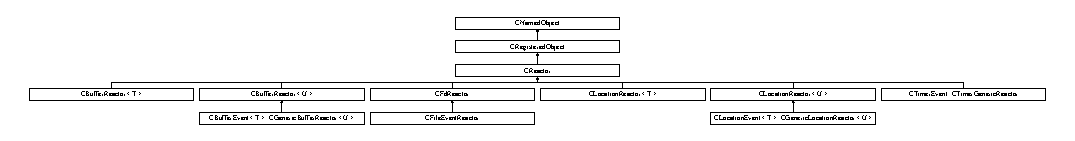
\includegraphics[height=1.44033cm]{classCReactor}
\end{center}
\end{figure}
\subsection*{Public Methods}
\begin{CompactItemize}
\item 
{\bf CReactor} ()
\item 
{\bf CReactor} (const string \&r\-Name)
\item 
{\bf CReactor} (const char $\ast$p\-Name)
\item 
virtual {\bf $\sim$CReactor} ()
\item 
int {\bf operator==} (const CReactor \&a\-CReactor) const
\item 
virtual void {\bf operator()} ({\bf CEvent\-Monitor} \&r\-Monitor, {\bf CEvent\-Monitor::result} Reason)
\item 
virtual void {\bf On\-Event} ({\bf CEvent\-Monitor} \&r\-Monitor)
\item 
virtual void {\bf On\-Error} ({\bf CEvent\-Monitor} \&r\-Monitor)
\item 
virtual void {\bf On\-Timeout} ({\bf CEvent\-Monitor} \&r\-Monitor)
\end{CompactItemize}
\subsection*{Private Methods}
\begin{CompactItemize}
\item 
{\bf CReactor} (const CReactor \&a\-CReactor)
\begin{CompactList}\small\item\em For now copy construction is not allowed.\item\end{CompactList}\item 
CReactor \& {\bf operator=} (const CReactor \&a\-CReactor)
\begin{CompactList}\small\item\em For now assignment is illegal.\item\end{CompactList}\end{CompactItemize}


\subsection{Detailed Description}
Encapsulates the base class for reactors. A reactor is an object which responds to an  event. This class hierarchy is of necessity slightly parallel to the Monitor hierarchy. In additional to the Named Object standard functions, all monitors must implement:\begin{CompactItemize}
\item 
operator() - called when the monitor fires.\end{CompactItemize}
\begin{CompactItemize}
\item 
{\bf On\-Event}() {\rm (p.\,\pageref{classCReactor_a6})} - Called from operator() if an event fired.\item 
{\bf On\-Error}() {\rm (p.\,\pageref{classCReactor_a7})} - Called from operator() if a monitor detected and error.\item 
{\bf On\-Timeout}() {\rm (p.\,\pageref{classCReactor_a8})}- Called from operator() if a monitor deteted a timeout.\end{CompactItemize}
As a named object, CReactor's require a name on construction. The name is entered into the \char`\"{}Reactor\char`\"{} registry. As a convenience, a default  constructor is supplied, however. If used the default constructor generates a name of the form Reactor\_\-nnn where nnn is a unique number... from m\_\-Auto\-Index.

This base class provides: Get\-Auto\-Name member function for derived classes which desire to implement this functionality as well. 



Definition at line 331 of file CReactor.h.

\subsection{Constructor \& Destructor Documentation}
\index{CReactor@{CReactor}!CReactor@{CReactor}}
\index{CReactor@{CReactor}!CReactor@{CReactor}}
\subsubsection{\setlength{\rightskip}{0pt plus 5cm}CReactor::CReactor ()}\label{classCReactor_a0}


Default constructor. A Reactor with name of the form Reactor\_\-nnn is created. The reactor is entered in to the \char`\"{}Reactor\char`\"{} registry of the  classified object registry returned from get\-CClassified\-Object\-Registry(). The name used is gaurenteed unique and can be queried via: {\bf get\-Name}() {\rm (p.\,\pageref{classCNamedObject_a6})}. 

Definition at line 321 of file CReactor.cpp.

References CNamed\-Object::Append\-Class\-Info(), and Registry\-Name.\index{CReactor@{CReactor}!CReactor@{CReactor}}
\index{CReactor@{CReactor}!CReactor@{CReactor}}
\subsubsection{\setlength{\rightskip}{0pt plus 5cm}CReactor::CReactor (const string \& {\em r\-Name})}\label{classCReactor_a1}


Constructs a Reactor given a name as an STL string:\begin{Desc}
\item[Parameters: ]\par
\begin{description}
\item[{\em 
r\-Name}]- The desired name of the reactor.\end{description}
\end{Desc}
Throws:\begin{CompactItemize}
\item 
{\bf CDuplicate\-Name\-Exception} {\rm (p.\,\pageref{classCDuplicateNameException})} (indirectly) if a Reactor of this name already exists. \end{CompactItemize}


Definition at line 337 of file CReactor.cpp.

References CNamed\-Object::Append\-Class\-Info(), and Registry\-Name.\index{CReactor@{CReactor}!CReactor@{CReactor}}
\index{CReactor@{CReactor}!CReactor@{CReactor}}
\subsubsection{\setlength{\rightskip}{0pt plus 5cm}CReactor::CReactor (const char $\ast$ {\em p\-Name})}\label{classCReactor_a2}


Constructs a reactor given its name as an ASCIZ string:\begin{Desc}
\item[Parameters: ]\par
\begin{description}
\item[{\em 
p\-Name}]- char$\ast$ pointer to the desired object name.\end{description}
\end{Desc}
Throws: -{\bf CDuplicate\-Name\-Exception} {\rm (p.\,\pageref{classCDuplicateNameException})} (indirectly) if a Reactor of this name already exists. 

Definition at line 354 of file CReactor.cpp.

References CNamed\-Object::Append\-Class\-Info(), and Registry\-Name.\index{CReactor@{CReactor}!CReactor@{CReactor}}
\index{CReactor@{CReactor}!CReactor@{CReactor}}
\subsubsection{\setlength{\rightskip}{0pt plus 5cm}CReactor::CReactor (const CReactor \& {\em a\-CReactor})\hspace{0.3cm}{\tt  [private]}}\label{classCReactor_c0}


For now copy construction is not allowed.

\index{CReactor@{CReactor}!~CReactor@{$\sim$CReactor}}
\index{~CReactor@{$\sim$CReactor}!CReactor@{CReactor}}
\subsubsection{\setlength{\rightskip}{0pt plus 5cm}CReactor::$\sim$CReactor ()\hspace{0.3cm}{\tt  [virtual]}}\label{classCReactor_a3}


Destructor: Just ensure that we are removed from the Reactors registry before being destroyed. 

Definition at line 366 of file CReactor.cpp.

References CApplication\-Registry::get\-Instance(), Registry\-Name, and CClassified\-Object\-Registry::Remove().

\subsection{Member Function Documentation}
\index{CReactor@{CReactor}!OnError@{OnError}}
\index{OnError@{OnError}!CReactor@{CReactor}}
\subsubsection{\setlength{\rightskip}{0pt plus 5cm}void CReactor::On\-Error ({\bf CEvent\-Monitor} \& {\em r\-Event})\hspace{0.3cm}{\tt  [virtual]}}\label{classCReactor_a7}


Called when the event monitor detects an error while waiting for an event. In general, this class is subclassed, and the actual code for On\-Error is supplied by the subclass. In order to support classes which may not care about event monitor errors themselves,  we provide an empty implementation of this function, preventing us from being an ABC.\begin{Desc}
\item[Parameters: ]\par
\begin{description}
\item[{\em 
r\-Monitor}]- The monitor which detected the event. \end{description}
\end{Desc}


Definition at line 447 of file CReactor.cpp.

Referenced by operator()().\index{CReactor@{CReactor}!OnEvent@{OnEvent}}
\index{OnEvent@{OnEvent}!CReactor@{CReactor}}
\subsubsection{\setlength{\rightskip}{0pt plus 5cm}void CReactor::On\-Event ({\bf CEvent\-Monitor} \& {\em r\-Event})\hspace{0.3cm}{\tt  [virtual]}}\label{classCReactor_a6}


Called when the event occurs. This is called from operator(). In general, this class is subclassed, and the actual code for On\-Event is supplied by the subclass. In order to support classes which may not care about the event themselves, we provide an empty implementation of this function, preventing us from being an ABC.\begin{Desc}
\item[Parameters: ]\par
\begin{description}
\item[{\em 
r\-Monitor}]- The monitor which detected the event. \end{description}
\end{Desc}


Reimplemented in {\bf CBuffer\-Reactor$<$ T $>$} {\rm (p.\,\pageref{classCBufferReactor_a5})}, {\bf CFd\-Reactor} {\rm (p.\,\pageref{classCFdReactor_a5})}, {\bf CLocation\-Reactor$<$ T $>$} {\rm (p.\,\pageref{classCLocationReactor_a5})}, {\bf CTimer\-Event::CTimer\-Generic\-Reactor} {\rm (p.\,\pageref{classCTimerEvent_1_1CTimerGenericReactor_a2})}, {\bf CBuffer\-Reactor$<$ U $>$} {\rm (p.\,\pageref{classCBufferReactor_a5})}, and {\bf CLocation\-Reactor$<$ U $>$} {\rm (p.\,\pageref{classCLocationReactor_a5})}.

Definition at line 433 of file CReactor.cpp.

Referenced by operator()().\index{CReactor@{CReactor}!OnTimeout@{OnTimeout}}
\index{OnTimeout@{OnTimeout}!CReactor@{CReactor}}
\subsubsection{\setlength{\rightskip}{0pt plus 5cm}void CReactor::On\-Timeout ({\bf CEvent\-Monitor} \& {\em r\-Event})\hspace{0.3cm}{\tt  [virtual]}}\label{classCReactor_a8}


Called when an event monitor detects a timeout while waiting for the event. In general, this class is subclassed, and the actual code for On\-Timeout is supplied by the subclass. In order to support classes which may not care about event monitor timeouts themselves,  we provide an empty implementation of this function, preventing us from being an ABC.\begin{Desc}
\item[Parameters: ]\par
\begin{description}
\item[{\em 
r\-Monitor}]- The monitor which detected the event. \end{description}
\end{Desc}


Reimplemented in {\bf CBuffer\-Event$<$ T $>$::CGeneric\-Buffer\-Reactor$<$ U $>$} {\rm (p.\,\pageref{classCBufferEvent_1_1CGenericBufferReactor_a2})}, {\bf CFile\-Event\-Reactor} {\rm (p.\,\pageref{classCFileEvent_1_1CFileEventReactor_a5})}, {\bf CLocation\-Event$<$ T $>$::CGeneric\-Location\-Reactor$<$ U $>$} {\rm (p.\,\pageref{classCLocationEvent_1_1CGenericLocationReactor_a2})}, and {\bf CBuffer\-Event$<$ T $>$::CGeneric\-Buffer\-Reactor$<$ T $>$} {\rm (p.\,\pageref{classCBufferEvent_1_1CGenericBufferReactor_a2})}.

Definition at line 461 of file CReactor.cpp.

Referenced by operator()().\index{CReactor@{CReactor}!operator()@{operator()}}
\index{operator()@{operator()}!CReactor@{CReactor}}
\subsubsection{\setlength{\rightskip}{0pt plus 5cm}void CReactor::operator() ({\bf CEvent\-Monitor} \& {\em r\-Monitor}, {\bf CEvent\-Monitor::result} {\em Reason})\hspace{0.3cm}{\tt  [virtual]}}\label{classCReactor_a5}


Operation Type: Interface Definition

Purpose:

This method is called in response ot an event from an event monitor on which this reactor has been established. The Reactor provides  application specific procesing of the event.\begin{Desc}
\item[Parameters: ]\par
\begin{description}
\item[{\em 
r\-Monitor}]- The event monitor which fired off our reaction. \item[{\em 
Reason}]- Why we were fired. Can be any of:\begin{CompactItemize}
\item 
Ocurred - the event happened.\item 
Timed\-Out - The event did not happen within the timeout.\item 
Error - Some error occured on the event.\end{CompactItemize}
\end{description}
\end{Desc}
Throws:\begin{CompactItemize}
\item 
{\bf CRange\-Error} {\rm (p.\,\pageref{classCRangeError})} if an invalid Reason was passed in. \end{CompactItemize}


Definition at line 404 of file CReactor.cpp.

References CEvent\-Monitor::Error, CEvent\-Monitor::Occurred, On\-Error(), On\-Event(), On\-Timeout(), CEvent\-Monitor::result, and CEvent\-Monitor::Timed\-Out.\index{CReactor@{CReactor}!operator=@{operator=}}
\index{operator=@{operator=}!CReactor@{CReactor}}
\subsubsection{\setlength{\rightskip}{0pt plus 5cm}CReactor\& CReactor::operator= (const CReactor \& {\em a\-CReactor})\hspace{0.3cm}{\tt  [private]}}\label{classCReactor_c1}


For now assignment is illegal.

\index{CReactor@{CReactor}!operator==@{operator==}}
\index{operator==@{operator==}!CReactor@{CReactor}}
\subsubsection{\setlength{\rightskip}{0pt plus 5cm}int CReactor::operator== (const CReactor \& {\em a\-CReactor}) const}\label{classCReactor_a4}




Definition at line 374 of file CReactor.cpp.

References CRegistered\-Object::operator==().

Referenced by CLocation\-Reactor$<$ T $>$::operator==(), CFd\-Reactor::operator==(), and CBuffer\-Reactor$<$ T $>$::operator==().

The documentation for this class was generated from the following files:\begin{CompactItemize}
\item 
{\bf CReactor.h}\item 
{\bf CReactor.cpp}\end{CompactItemize}

\section{CRefcounted\-Ptr$<$ T $>$  Class Template Reference}
\label{classCRefcountedPtr}\index{CRefcountedPtr@{CRefcounted\-Ptr}}
{\tt \#include $<$CRefptr.h$>$}

\subsection*{Public Methods}
\begin{CompactItemize}
\item 
{\bf CRefcounted\-Ptr} ()
\item 
{\bf CRefcounted\-Ptr} (T $\ast$p)
\item 
{\bf $\sim$CRefcounted\-Ptr} ()
\item 
template$<$class U$>$ {\bf CRefcounted\-Ptr} (const CRefcounted\-Ptr$<$ U $>$ \&rhs)
\item 
CRefcounted\-Ptr \& {\bf operator=} (const CRefcounted\-Ptr \&rhs)
\item 
int {\bf refcount} () const
\item 
template$<$class U$>$ int {\bf operator==} (const CRefcounted\-Ptr$<$ U $>$ \&rhs)
\item 
T \& {\bf operator $\ast$} ()
\item 
T $\ast$ {\bf operator $\rightarrow$ } ()
\end{CompactItemize}
\subsection*{Private Attributes}
\begin{CompactItemize}
\item 
{\bf CReference\-Counted}$<$ T $>$ $\ast$ {\bf m\_\-Object}
\end{CompactItemize}
\subsubsection*{template$<$class T$>$ class CRefcounted\-Ptr$<$ T $>$}



\subsection{Constructor \& Destructor Documentation}
\index{CRefcountedPtr@{CRefcounted\-Ptr}!CRefcountedPtr@{CRefcountedPtr}}
\index{CRefcountedPtr@{CRefcountedPtr}!CRefcountedPtr@{CRefcounted\-Ptr}}
\subsubsection{\setlength{\rightskip}{0pt plus 5cm}template$<$class T$>$ CRefcounted\-Ptr$<$ T $>$::CRefcounted\-Ptr ()\hspace{0.3cm}{\tt  [inline]}}\label{classCRefcountedPtr_a0}




Definition at line 326 of file CRefptr.h.\index{CRefcountedPtr@{CRefcounted\-Ptr}!CRefcountedPtr@{CRefcountedPtr}}
\index{CRefcountedPtr@{CRefcountedPtr}!CRefcountedPtr@{CRefcounted\-Ptr}}
\subsubsection{\setlength{\rightskip}{0pt plus 5cm}template$<$class T$>$ CRefcounted\-Ptr$<$ T $>$::CRefcounted\-Ptr (T $\ast$ {\em p})\hspace{0.3cm}{\tt  [inline]}}\label{classCRefcountedPtr_a1}




Definition at line 327 of file CRefptr.h.\index{CRefcountedPtr@{CRefcounted\-Ptr}!~CRefcountedPtr@{$\sim$CRefcountedPtr}}
\index{~CRefcountedPtr@{$\sim$CRefcountedPtr}!CRefcountedPtr@{CRefcounted\-Ptr}}
\subsubsection{\setlength{\rightskip}{0pt plus 5cm}template$<$class T$>$ CRefcounted\-Ptr$<$ T $>$::$\sim$CRefcounted\-Ptr ()\hspace{0.3cm}{\tt  [inline]}}\label{classCRefcountedPtr_a2}




Definition at line 329 of file CRefptr.h.

References CReference\-Counted$<$ T $>$::dereference(), and CReference\-Counted$<$ T $>$::norefs().\index{CRefcountedPtr@{CRefcounted\-Ptr}!CRefcountedPtr@{CRefcountedPtr}}
\index{CRefcountedPtr@{CRefcountedPtr}!CRefcountedPtr@{CRefcounted\-Ptr}}
\subsubsection{\setlength{\rightskip}{0pt plus 5cm}template$<$class T$>$ template$<$class U$>$ CRefcounted\-Ptr$<$ T $>$::CRefcounted\-Ptr (const CRefcounted\-Ptr$<$ U $>$ \& {\em rhs})\hspace{0.3cm}{\tt  [inline]}}\label{classCRefcountedPtr_a3}




Definition at line 336 of file CRefptr.h.

References CRefcounted\-Ptr$<$ T $>$::m\_\-Object, and CReference\-Counted$<$ T $>$::reference().

\subsection{Member Function Documentation}
\index{CRefcountedPtr@{CRefcounted\-Ptr}!operator *@{operator $\ast$}}
\index{operator *@{operator $\ast$}!CRefcountedPtr@{CRefcounted\-Ptr}}
\subsubsection{\setlength{\rightskip}{0pt plus 5cm}template$<$class T$>$ T\& CRefcounted\-Ptr$<$ T $>$::operator $\ast$ ()\hspace{0.3cm}{\tt  [inline]}}\label{classCRefcountedPtr_a7}




Definition at line 372 of file CRefptr.h.\index{CRefcountedPtr@{CRefcounted\-Ptr}!operator->@{operator-$>$}}
\index{operator->@{operator-$>$}!CRefcountedPtr@{CRefcounted\-Ptr}}
\subsubsection{\setlength{\rightskip}{0pt plus 5cm}template$<$class T$>$ T$\ast$ CRefcounted\-Ptr$<$ T $>$::operator $\rightarrow$  ()\hspace{0.3cm}{\tt  [inline]}}\label{classCRefcountedPtr_a8}




Definition at line 373 of file CRefptr.h.

References CReference\-Counted$<$ T $>$::get().\index{CRefcountedPtr@{CRefcounted\-Ptr}!operator=@{operator=}}
\index{operator=@{operator=}!CRefcountedPtr@{CRefcounted\-Ptr}}
\subsubsection{\setlength{\rightskip}{0pt plus 5cm}template$<$class T$>$ CRefcounted\-Ptr\& CRefcounted\-Ptr$<$ T $>$::operator= (const CRefcounted\-Ptr$<$ T $>$ \& {\em rhs})\hspace{0.3cm}{\tt  [inline]}}\label{classCRefcountedPtr_a4}




Definition at line 343 of file CRefptr.h.

References CReference\-Counted$<$ T $>$::dereference(), CRefcounted\-Ptr$<$ T $>$::m\_\-Object, CReference\-Counted$<$ T $>$::norefs(), and CReference\-Counted$<$ T $>$::reference().\index{CRefcountedPtr@{CRefcounted\-Ptr}!operator==@{operator==}}
\index{operator==@{operator==}!CRefcountedPtr@{CRefcounted\-Ptr}}
\subsubsection{\setlength{\rightskip}{0pt plus 5cm}template$<$class T$>$ template$<$class U$>$ int CRefcounted\-Ptr$<$ T $>$::operator== (const CRefcounted\-Ptr$<$ U $>$ \& {\em rhs})\hspace{0.3cm}{\tt  [inline]}}\label{classCRefcountedPtr_a6}




Definition at line 369 of file CRefptr.h.

References CRefcounted\-Ptr$<$ T $>$::m\_\-Object.\index{CRefcountedPtr@{CRefcounted\-Ptr}!refcount@{refcount}}
\index{refcount@{refcount}!CRefcountedPtr@{CRefcounted\-Ptr}}
\subsubsection{\setlength{\rightskip}{0pt plus 5cm}template$<$class T$>$ int CRefcounted\-Ptr$<$ T $>$::refcount () const\hspace{0.3cm}{\tt  [inline]}}\label{classCRefcountedPtr_a5}




Definition at line 358 of file CRefptr.h.

References CReference\-Counted$<$ T $>$::refcount().

\subsection{Member Data Documentation}
\index{CRefcountedPtr@{CRefcounted\-Ptr}!m_Object@{m\_\-Object}}
\index{m_Object@{m\_\-Object}!CRefcountedPtr@{CRefcounted\-Ptr}}
\subsubsection{\setlength{\rightskip}{0pt plus 5cm}template$<$class T$>$ {\bf CReference\-Counted}$<$T$>$$\ast$ CRefcounted\-Ptr$<$ T $>$::m\_\-Object\hspace{0.3cm}{\tt  [private]}}\label{classCRefcountedPtr_o0}




Definition at line 324 of file CRefptr.h.

Referenced by CRefcounted\-Ptr$<$ T $>$::CRefcounted\-Ptr(), CRefcounted\-Ptr$<$ T $>$::operator=(), and CRefcounted\-Ptr$<$ T $>$::operator==().

The documentation for this class was generated from the following file:\begin{CompactItemize}
\item 
{\bf CRefptr.h}\end{CompactItemize}

\section{CReference\-Counted$<$ T $>$  Class Template Reference}
\label{classCReferenceCounted}\index{CReferenceCounted@{CReference\-Counted}}
{\tt \#include $<$CRefptr.h$>$}

\subsection*{Public Methods}
\begin{CompactItemize}
\item 
{\bf CReference\-Counted} (T $\ast$p)
\item 
{\bf $\sim$CReference\-Counted} ()
\item 
T \& {\bf operator $\ast$} ()
\item 
T $\ast$ {\bf get} ()
\item 
void {\bf reference} ()
\item 
void {\bf dereference} ()
\item 
int {\bf norefs} ()
\item 
int {\bf refcount} ()
\end{CompactItemize}
\subsection*{Private Methods}
\begin{CompactItemize}
\item 
template$<$class U$>$ CReference\-Counted$<$ T $>$ \& {\bf operator=} (const CReference\-Counted$<$ U $>$ \&rhs)
\item 
template$<$class U$>$ {\bf CReference\-Counted} (const CReference\-Counted$<$ U $>$ \&rhs)
\end{CompactItemize}
\subsection*{Private Attributes}
\begin{CompactItemize}
\item 
unsigned {\bf m\_\-Reference\-Count}
\item 
T $\ast$ {\bf m\_\-Pointer}
\end{CompactItemize}
\subsubsection*{template$<$class T$>$ class CReference\-Counted$<$ T $>$}



\subsection{Constructor \& Destructor Documentation}
\index{CReferenceCounted@{CReference\-Counted}!CReferenceCounted@{CReferenceCounted}}
\index{CReferenceCounted@{CReferenceCounted}!CReferenceCounted@{CReference\-Counted}}
\subsubsection{\setlength{\rightskip}{0pt plus 5cm}template$<$class T$>$ template$<$class U$>$ CReference\-Counted$<$ T $>$::CReference\-Counted (const CReference\-Counted$<$ U $>$ \& {\em rhs})\hspace{0.3cm}{\tt  [private]}}\label{classCReferenceCounted_c1}


\index{CReferenceCounted@{CReference\-Counted}!CReferenceCounted@{CReferenceCounted}}
\index{CReferenceCounted@{CReferenceCounted}!CReferenceCounted@{CReference\-Counted}}
\subsubsection{\setlength{\rightskip}{0pt plus 5cm}template$<$class T$>$ CReference\-Counted$<$ T $>$::CReference\-Counted (T $\ast$ {\em p})\hspace{0.3cm}{\tt  [inline]}}\label{classCReferenceCounted_a0}




Definition at line 307 of file CRefptr.h.

References CReference\-Counted$<$ T $>$::m\_\-Pointer, and CReference\-Counted$<$ T $>$::m\_\-Reference\-Count.\index{CReferenceCounted@{CReference\-Counted}!~CReferenceCounted@{$\sim$CReferenceCounted}}
\index{~CReferenceCounted@{$\sim$CReferenceCounted}!CReferenceCounted@{CReference\-Counted}}
\subsubsection{\setlength{\rightskip}{0pt plus 5cm}template$<$class T$>$ CReference\-Counted$<$ T $>$::$\sim$CReference\-Counted ()\hspace{0.3cm}{\tt  [inline]}}\label{classCReferenceCounted_a1}




Definition at line 310 of file CRefptr.h.

References CReference\-Counted$<$ T $>$::m\_\-Pointer.

\subsection{Member Function Documentation}
\index{CReferenceCounted@{CReference\-Counted}!dereference@{dereference}}
\index{dereference@{dereference}!CReferenceCounted@{CReference\-Counted}}
\subsubsection{\setlength{\rightskip}{0pt plus 5cm}template$<$class T$>$ void CReference\-Counted$<$ T $>$::dereference ()\hspace{0.3cm}{\tt  [inline]}}\label{classCReferenceCounted_a5}




Definition at line 314 of file CRefptr.h.

References CReference\-Counted$<$ T $>$::m\_\-Reference\-Count.

Referenced by CRefcounted\-Ptr$<$ T $>$::operator=(), and CRefcounted\-Ptr$<$ T $>$::$\sim$CRefcounted\-Ptr().\index{CReferenceCounted@{CReference\-Counted}!get@{get}}
\index{get@{get}!CReferenceCounted@{CReference\-Counted}}
\subsubsection{\setlength{\rightskip}{0pt plus 5cm}template$<$class T$>$ T$\ast$ CReference\-Counted$<$ T $>$::get ()\hspace{0.3cm}{\tt  [inline]}}\label{classCReferenceCounted_a3}




Definition at line 312 of file CRefptr.h.

References CReference\-Counted$<$ T $>$::m\_\-Pointer.

Referenced by CRefcounted\-Ptr$<$ T $>$::operator $\rightarrow$ ().\index{CReferenceCounted@{CReference\-Counted}!norefs@{norefs}}
\index{norefs@{norefs}!CReferenceCounted@{CReference\-Counted}}
\subsubsection{\setlength{\rightskip}{0pt plus 5cm}template$<$class T$>$ int CReference\-Counted$<$ T $>$::norefs ()\hspace{0.3cm}{\tt  [inline]}}\label{classCReferenceCounted_a6}




Definition at line 315 of file CRefptr.h.

References CReference\-Counted$<$ T $>$::m\_\-Reference\-Count.

Referenced by CRefcounted\-Ptr$<$ T $>$::operator=(), and CRefcounted\-Ptr$<$ T $>$::$\sim$CRefcounted\-Ptr().\index{CReferenceCounted@{CReference\-Counted}!operator *@{operator $\ast$}}
\index{operator *@{operator $\ast$}!CReferenceCounted@{CReference\-Counted}}
\subsubsection{\setlength{\rightskip}{0pt plus 5cm}template$<$class T$>$ T\& CReference\-Counted$<$ T $>$::operator $\ast$ ()\hspace{0.3cm}{\tt  [inline]}}\label{classCReferenceCounted_a2}




Definition at line 311 of file CRefptr.h.

References CReference\-Counted$<$ T $>$::m\_\-Pointer.\index{CReferenceCounted@{CReference\-Counted}!operator=@{operator=}}
\index{operator=@{operator=}!CReferenceCounted@{CReference\-Counted}}
\subsubsection{\setlength{\rightskip}{0pt plus 5cm}template$<$class T$>$ template$<$class U$>$ CReference\-Counted$<$T$>$\& CReference\-Counted$<$ T $>$::operator= (const CReference\-Counted$<$ U $>$ \& {\em rhs})\hspace{0.3cm}{\tt  [private]}}\label{classCReferenceCounted_c0}


\index{CReferenceCounted@{CReference\-Counted}!refcount@{refcount}}
\index{refcount@{refcount}!CReferenceCounted@{CReference\-Counted}}
\subsubsection{\setlength{\rightskip}{0pt plus 5cm}template$<$class T$>$ int CReference\-Counted$<$ T $>$::refcount ()\hspace{0.3cm}{\tt  [inline]}}\label{classCReferenceCounted_a7}




Definition at line 316 of file CRefptr.h.

References CReference\-Counted$<$ T $>$::m\_\-Reference\-Count.

Referenced by CRefcounted\-Ptr$<$ T $>$::refcount().\index{CReferenceCounted@{CReference\-Counted}!reference@{reference}}
\index{reference@{reference}!CReferenceCounted@{CReference\-Counted}}
\subsubsection{\setlength{\rightskip}{0pt plus 5cm}template$<$class T$>$ void CReference\-Counted$<$ T $>$::reference ()\hspace{0.3cm}{\tt  [inline]}}\label{classCReferenceCounted_a4}




Definition at line 313 of file CRefptr.h.

References CReference\-Counted$<$ T $>$::m\_\-Reference\-Count.

Referenced by CRefcounted\-Ptr$<$ T $>$::CRefcounted\-Ptr(), and CRefcounted\-Ptr$<$ T $>$::operator=().

\subsection{Member Data Documentation}
\index{CReferenceCounted@{CReference\-Counted}!m_Pointer@{m\_\-Pointer}}
\index{m_Pointer@{m\_\-Pointer}!CReferenceCounted@{CReference\-Counted}}
\subsubsection{\setlength{\rightskip}{0pt plus 5cm}template$<$class T$>$ T$\ast$ CReference\-Counted$<$ T $>$::m\_\-Pointer\hspace{0.3cm}{\tt  [private]}}\label{classCReferenceCounted_o1}




Definition at line 298 of file CRefptr.h.

Referenced by CReference\-Counted$<$ T $>$::CReference\-Counted(), CReference\-Counted$<$ T $>$::get(), CReference\-Counted$<$ T $>$::operator $\ast$(), and CReference\-Counted$<$ T $>$::$\sim$CReference\-Counted().\index{CReferenceCounted@{CReference\-Counted}!m_ReferenceCount@{m\_\-ReferenceCount}}
\index{m_ReferenceCount@{m\_\-ReferenceCount}!CReferenceCounted@{CReference\-Counted}}
\subsubsection{\setlength{\rightskip}{0pt plus 5cm}template$<$class T$>$ unsigned CReference\-Counted$<$ T $>$::m\_\-Reference\-Count\hspace{0.3cm}{\tt  [private]}}\label{classCReferenceCounted_o0}




Definition at line 297 of file CRefptr.h.

Referenced by CReference\-Counted$<$ T $>$::CReference\-Counted(), CReference\-Counted$<$ T $>$::dereference(), CReference\-Counted$<$ T $>$::norefs(), CReference\-Counted$<$ T $>$::refcount(), and CReference\-Counted$<$ T $>$::reference().

The documentation for this class was generated from the following file:\begin{CompactItemize}
\item 
{\bf CRefptr.h}\end{CompactItemize}

\section{CRegistered\-Object  Class Reference}
\label{classCRegisteredObject}\index{CRegisteredObject@{CRegistered\-Object}}
{\tt \#include $<$CRegistered\-Object.h$>$}

Inheritance diagram for CRegistered\-Object::\begin{figure}[H]
\begin{center}
\leavevmode
\includegraphics[height=2.77533cm]{classCRegisteredObject}
\end{center}
\end{figure}
\subsection*{Public Methods}
\begin{CompactItemize}
\item 
{\bf CRegistered\-Object} (string am\_\-s\-Name, {\bf CClassified\-Object\-Registry} $\ast$am\_\-Registry, const string \&{\bf Registry\-Name})
\item 
int {\bf operator==} (const CRegistered\-Object \&a\-CRegistered\-Object) const
\item 
virtual {\bf $\sim$CRegistered\-Object} ()
\item 
const {\bf CClassified\-Object\-Registry} $\ast$ {\bf get\-Registry} () const
\item 
void {\bf Register\-Self} (const string \&{\bf Registry\-Name})
\end{CompactItemize}
\subsection*{Protected Methods}
\begin{CompactItemize}
\item 
void {\bf set\-Registry} ({\bf CClassified\-Object\-Registry} $\ast$const am\_\-Registry)
\end{CompactItemize}
\subsection*{Private Methods}
\begin{CompactItemize}
\item 
{\bf CRegistered\-Object} (const CRegistered\-Object \&a\-CRegistered\-Object)
\begin{CompactList}\small\item\em Copy construction is forbidden for now.\item\end{CompactList}\item 
CRegistered\-Object {\bf operator=} (const CRegistered\-Object \&a\-CRegistered\-Object)
\begin{CompactList}\small\item\em Assignment is forbidden for now.\item\end{CompactList}\end{CompactItemize}
\subsection*{Private Attributes}
\begin{CompactItemize}
\item 
{\bf CClassified\-Object\-Registry} $\ast$ {\bf m\_\-Registry}
\end{CompactItemize}


\subsection{Detailed Description}
Registered\-Object.h:

This file defines the CRegistered\-Object class.

Author: Jason Venema NSCL Michigan State University East Lansing, MI 48824-1321 mailto:{\tt venemaja@msu.edu} 



Definition at line 307 of file CRegistered\-Object.h.

\subsection{Constructor \& Destructor Documentation}
\index{CRegisteredObject@{CRegistered\-Object}!CRegisteredObject@{CRegisteredObject}}
\index{CRegisteredObject@{CRegisteredObject}!CRegisteredObject@{CRegistered\-Object}}
\subsubsection{\setlength{\rightskip}{0pt plus 5cm}CRegistered\-Object::CRegistered\-Object (string {\em am\_\-s\-Name}, {\bf CClassified\-Object\-Registry} $\ast$ {\em am\_\-Registry}, const string \& {\em Registry\-Name})\hspace{0.3cm}{\tt  [inline]}}\label{classCRegisteredObject_a0}


The classified object  registry into which this  object will be registered 

Definition at line 315 of file CRegistered\-Object.h.

References CNamed\-Object::Append\-Class\-Info(), and Register\-Self().\index{CRegisteredObject@{CRegistered\-Object}!CRegisteredObject@{CRegisteredObject}}
\index{CRegisteredObject@{CRegisteredObject}!CRegisteredObject@{CRegistered\-Object}}
\subsubsection{\setlength{\rightskip}{0pt plus 5cm}CRegistered\-Object::CRegistered\-Object (const CRegistered\-Object \& {\em a\-CRegistered\-Object})\hspace{0.3cm}{\tt  [private]}}\label{classCRegisteredObject_c0}


Copy construction is forbidden for now.

\index{CRegisteredObject@{CRegistered\-Object}!~CRegisteredObject@{$\sim$CRegisteredObject}}
\index{~CRegisteredObject@{$\sim$CRegisteredObject}!CRegisteredObject@{CRegistered\-Object}}
\subsubsection{\setlength{\rightskip}{0pt plus 5cm}virtual CRegistered\-Object::$\sim$CRegistered\-Object ()\hspace{0.3cm}{\tt  [inline, virtual]}}\label{classCRegisteredObject_a2}




Definition at line 339 of file CRegistered\-Object.h.

\subsection{Member Function Documentation}
\index{CRegisteredObject@{CRegistered\-Object}!getRegistry@{getRegistry}}
\index{getRegistry@{getRegistry}!CRegisteredObject@{CRegistered\-Object}}
\subsubsection{\setlength{\rightskip}{0pt plus 5cm}const {\bf CClassified\-Object\-Registry}$\ast$ CRegistered\-Object::get\-Registry () const\hspace{0.3cm}{\tt  [inline]}}\label{classCRegisteredObject_a3}




Definition at line 344 of file CRegistered\-Object.h.

Referenced by CEvent\-Monitor::$\sim$CEvent\-Monitor().\index{CRegisteredObject@{CRegistered\-Object}!operator=@{operator=}}
\index{operator=@{operator=}!CRegisteredObject@{CRegistered\-Object}}
\subsubsection{\setlength{\rightskip}{0pt plus 5cm}CRegistered\-Object CRegistered\-Object::operator= (const CRegistered\-Object \& {\em a\-CRegistered\-Object})\hspace{0.3cm}{\tt  [private]}}\label{classCRegisteredObject_c1}


Assignment is forbidden for now.



Reimplemented in {\bf CEvent\-Monitor} {\rm (p.\,\pageref{classCEventMonitor_c1})}, and {\bf CFd\-Monitor} {\rm (p.\,\pageref{classCFdMonitor_c1})}.\index{CRegisteredObject@{CRegistered\-Object}!operator==@{operator==}}
\index{operator==@{operator==}!CRegisteredObject@{CRegistered\-Object}}
\subsubsection{\setlength{\rightskip}{0pt plus 5cm}int CRegistered\-Object::operator== (const CRegistered\-Object \& {\em a\-CRegistered\-Object}) const\hspace{0.3cm}{\tt  [inline]}}\label{classCRegisteredObject_a1}




Definition at line 332 of file CRegistered\-Object.h.

References m\_\-Registry, and CNamed\-Object::operator==().

Referenced by CReactor::operator==(), CPointer\-Predicate$<$ T $>$::operator==(), and CEvent\-Monitor::operator==().\index{CRegisteredObject@{CRegistered\-Object}!RegisterSelf@{RegisterSelf}}
\index{RegisterSelf@{RegisterSelf}!CRegisteredObject@{CRegistered\-Object}}
\subsubsection{\setlength{\rightskip}{0pt plus 5cm}void CRegistered\-Object::Register\-Self (const string \& {\em Registry\-Name})}\label{classCRegisteredObject_a4}


Registers this object in the appropriate object registry. Note: the object registry will throw a Duplicate\-Name\-Exception if there is already an object in our registry with that name. If necessary, the registry is created. Implicit parameters: m\_\-Registry - a static member which is the collection of object registries into which the object will be registered. m\_\-s\-Name - the name under which the object will be registered.\begin{Desc}
\item[Parameters: ]\par
\begin{description}
\item[{\em 
Registry\-Name}]The name of the registry in which to register the object \end{description}
\end{Desc}


Definition at line 307 of file CRegistered\-Object.cpp.

References CClassified\-Object\-Registry::Add(), CClassified\-Object\-Registry::Create\-Registry(), and m\_\-Registry.

Referenced by CRegistered\-Object().\index{CRegisteredObject@{CRegistered\-Object}!setRegistry@{setRegistry}}
\index{setRegistry@{setRegistry}!CRegisteredObject@{CRegistered\-Object}}
\subsubsection{\setlength{\rightskip}{0pt plus 5cm}void CRegistered\-Object::set\-Registry ({\bf CClassified\-Object\-Registry} $\ast$const {\em am\_\-Registry})\hspace{0.3cm}{\tt  [inline, protected]}}\label{classCRegisteredObject_b0}




Definition at line 352 of file CRegistered\-Object.h.

\subsection{Member Data Documentation}
\index{CRegisteredObject@{CRegistered\-Object}!m_Registry@{m\_\-Registry}}
\index{m_Registry@{m\_\-Registry}!CRegisteredObject@{CRegistered\-Object}}
\subsubsection{\setlength{\rightskip}{0pt plus 5cm}{\bf CClassified\-Object\-Registry}$\ast$ CRegistered\-Object::m\_\-Registry\hspace{0.3cm}{\tt  [private]}}\label{classCRegisteredObject_o0}




Definition at line 309 of file CRegistered\-Object.h.

Referenced by operator==(), and Register\-Self().

The documentation for this class was generated from the following files:\begin{CompactItemize}
\item 
{\bf CRegistered\-Object.h}\item 
{\bf CRegistered\-Object.cpp}\end{CompactItemize}

\section{CServer\-Connection\-Event  Class Reference}
\label{classCServerConnectionEvent}\index{CServerConnectionEvent@{CServer\-Connection\-Event}}
$\backslash$class: CServer\-Connection\-Event $\backslash$file: {\bf CServer\-Connection\-Event.h}. 


{\tt \#include $<$CServer\-Connection\-Event.h$>$}

Inheritance diagram for CServer\-Connection\-Event::\begin{figure}[H]
\begin{center}
\leavevmode
\includegraphics[height=5cm]{classCServerConnectionEvent}
\end{center}
\end{figure}
\subsection*{Public Methods}
\begin{CompactItemize}
\item 
{\bf CServer\-Connection\-Event} ({\bf CSocket} \&sock)
\item 
{\bf CServer\-Connection\-Event} (const char $\ast$p\-Name, {\bf CSocket} \&sock)
\item 
{\bf CServer\-Connection\-Event} (const string \&r\-Name, {\bf CSocket} \&sock)
\item 
{\bf CServer\-Connection\-Event} (const string \&r\-Service\-Name)
\item 
{\bf CServer\-Connection\-Event} (const char $\ast$p\-Name, const string \&r\-Service\-Name)
\item 
{\bf CServer\-Connection\-Event} (const string \&r\-Name, const string \&r\-Service\-Name)
\item 
{\bf CServer\-Connection\-Event} (int n\-Fd)
\item 
{\bf CServer\-Connection\-Event} (const char $\ast$p\-Name, int n\-Fd)
\item 
{\bf CServer\-Connection\-Event} (const string \&r\-Name, int n\-Fd)
\item 
{\bf $\sim$CServer\-Connection\-Event} ()
\item 
{\bf CSocket} $\ast$ {\bf get\-Socket} ()
\item 
bool {\bf is\-Dynamic\-Socket} () const
\item 
virtual void {\bf On\-Connection} ({\bf CSocket} $\ast$p\-Peer)
\item 
virtual void {\bf On\-Readable} (istream \&r\-Stream)
\item 
virtual string {\bf Describe\-Self} ()
\end{CompactItemize}
\subsection*{Protected Methods}
\begin{CompactItemize}
\item 
void {\bf set\-Socket} ({\bf CSocket} $\ast$p\-Socket)
\item 
void {\bf set\-Dynamic} (bool f\-Dyn)
\item 
void {\bf Configure\-Socket} (const string \&r\-Svc\-Name)
\item 
void {\bf Configure\-Socket} (int n\-Port)
\item 
int {\bf Protocol} ()
\end{CompactItemize}
\subsection*{Private Methods}
\begin{CompactItemize}
\item 
{\bf CServer\-Connection\-Event} (const CServer\-Connection\-Event \&rhs)
\item 
CServer\-Connection\-Event \& {\bf operator=} (const CServer\-Connection\-Event \&rhs)
\item 
int {\bf operator==} (const CServer\-Connection\-Event \&rhs)
\end{CompactItemize}
\subsection*{Private Attributes}
\begin{CompactItemize}
\item 
{\bf CSocket} $\ast$ {\bf m\_\-p\-Service}
\begin{CompactList}\small\item\em Server listener socket.\item\end{CompactList}\item 
bool {\bf m\_\-f\-Delete\-Socket}
\begin{CompactList}\small\item\em true if destructor delete socket.\item\end{CompactList}\end{CompactItemize}


\subsection{Detailed Description}
$\backslash$class: CServer\-Connection\-Event $\backslash$file: {\bf CServer\-Connection\-Event.h}.

This class encapsulates the process of listening for and accepting client connections to a Tcp/Ip service. The event is policy free in the sense that all it does is set up an encapsulated {\bf CSocket} {\rm (p.\,\pageref{classCSocket})} to listen on a specified port and listen for connections on the socket within a thread. When a connection request is received... it is accepted and the resulting socket is passed to {\bf On\-Connection}() {\rm (p.\,\pageref{classCServerConnectionEvent_a12})}

The user of this class in general will subclass the server and override the default (no-op) implementation of {\bf On\-Connection}() {\rm (p.\,\pageref{classCServerConnectionEvent_a12})} 



Definition at line 322 of file CServer\-Connection\-Event.h.

\subsection{Constructor \& Destructor Documentation}
\index{CServerConnectionEvent@{CServer\-Connection\-Event}!CServerConnectionEvent@{CServerConnectionEvent}}
\index{CServerConnectionEvent@{CServerConnectionEvent}!CServerConnectionEvent@{CServer\-Connection\-Event}}
\subsubsection{\setlength{\rightskip}{0pt plus 5cm}CServer\-Connection\-Event::CServer\-Connection\-Event ({\bf CSocket} \& {\em r\-Socket})}\label{classCServerConnectionEvent_a0}


Construct an anonymous connection listener from an existing socket object. In this case, it will not be necessary for the destructor to eliminate the socket.\begin{Desc}
\item[Parameters: ]\par
\begin{description}
\item[{\em 
sock}]- An existing socket, bound, listening and ready to accept when the fd becomes readable. \end{description}
\end{Desc}


Definition at line 305 of file CServer\-Connection\-Event.cpp.\index{CServerConnectionEvent@{CServer\-Connection\-Event}!CServerConnectionEvent@{CServerConnectionEvent}}
\index{CServerConnectionEvent@{CServerConnectionEvent}!CServerConnectionEvent@{CServer\-Connection\-Event}}
\subsubsection{\setlength{\rightskip}{0pt plus 5cm}CServer\-Connection\-Event::CServer\-Connection\-Event (const char $\ast$ {\em pname}, {\bf CSocket} \& {\em r\-Socket})}\label{classCServerConnectionEvent_a1}


Construct a named connection listener from and existing socket object.\begin{Desc}
\item[Parameters: ]\par
\begin{description}
\item[{\em 
p\-Name}]- char$\ast$ pointer to the name of the event. \item[{\em 
r\-Socket}]- Reference to existing socket. \end{description}
\end{Desc}


Definition at line 317 of file CServer\-Connection\-Event.cpp.\index{CServerConnectionEvent@{CServer\-Connection\-Event}!CServerConnectionEvent@{CServerConnectionEvent}}
\index{CServerConnectionEvent@{CServerConnectionEvent}!CServerConnectionEvent@{CServer\-Connection\-Event}}
\subsubsection{\setlength{\rightskip}{0pt plus 5cm}CServer\-Connection\-Event::CServer\-Connection\-Event (const string \& {\em r\-Name}, {\bf CSocket} \& {\em r\-Socket})}\label{classCServerConnectionEvent_a2}


Construct a named connnection listener from an existing socket object.\begin{Desc}
\item[Parameters: ]\par
\begin{description}
\item[{\em 
r\-Name}]- Reference to the object name desired. \item[{\em 
r\-Socket-}]Socket to create the listener around. The socket must be in the listening state, by the time the event is enabled/scheduled. \end{description}
\end{Desc}


Definition at line 331 of file CServer\-Connection\-Event.cpp.\index{CServerConnectionEvent@{CServer\-Connection\-Event}!CServerConnectionEvent@{CServerConnectionEvent}}
\index{CServerConnectionEvent@{CServerConnectionEvent}!CServerConnectionEvent@{CServer\-Connection\-Event}}
\subsubsection{\setlength{\rightskip}{0pt plus 5cm}CServer\-Connection\-Event::CServer\-Connection\-Event (const string \& {\em r\-Service\-Name})}\label{classCServerConnectionEvent_a3}


Construct an anonymous connection listener from a service name. Since we need to construct the file event with an fd, that will be done by an explicit socket(2) call. The m\_\-p\-Service will be dynamically allocated and configured from the fd, and the service information in the constructor body.\begin{Desc}
\item[Parameters: ]\par
\begin{description}
\item[{\em 
r\-Service\-Name}]- Name of the service to connect to. The {\bf CSocket} {\rm (p.\,\pageref{classCSocket})} type accepts either a name which translates via getservbyname, or a stringified service number. \end{description}
\end{Desc}


Definition at line 349 of file CServer\-Connection\-Event.cpp.

References Configure\-Socket().\index{CServerConnectionEvent@{CServer\-Connection\-Event}!CServerConnectionEvent@{CServerConnectionEvent}}
\index{CServerConnectionEvent@{CServerConnectionEvent}!CServerConnectionEvent@{CServer\-Connection\-Event}}
\subsubsection{\setlength{\rightskip}{0pt plus 5cm}CServer\-Connection\-Event::CServer\-Connection\-Event (const char $\ast$ {\em p\-Name}, const string \& {\em r\-Service\-Name})}\label{classCServerConnectionEvent_a4}


Construct a named connection listener from a service name. See above for more information. \begin{Desc}
\item[Parameters: ]\par
\begin{description}
\item[{\em 
p\-Name}]- char$\ast$ name to be given to the connection listener. \item[{\em 
r\-Service\-Name}]- Name of the service to connect to. The {\bf CSocket} {\rm (p.\,\pageref{classCSocket})} type accepts either a name which translates via getservbyname, or a stringified service number. \end{description}
\end{Desc}


Definition at line 365 of file CServer\-Connection\-Event.cpp.

References Configure\-Socket().\index{CServerConnectionEvent@{CServer\-Connection\-Event}!CServerConnectionEvent@{CServerConnectionEvent}}
\index{CServerConnectionEvent@{CServerConnectionEvent}!CServerConnectionEvent@{CServer\-Connection\-Event}}
\subsubsection{\setlength{\rightskip}{0pt plus 5cm}CServer\-Connection\-Event::CServer\-Connection\-Event (const string \& {\em r\-Name}, const string \& {\em r\-Service\-Name})}\label{classCServerConnectionEvent_a5}




Definition at line 373 of file CServer\-Connection\-Event.cpp.

References Configure\-Socket().\index{CServerConnectionEvent@{CServer\-Connection\-Event}!CServerConnectionEvent@{CServerConnectionEvent}}
\index{CServerConnectionEvent@{CServerConnectionEvent}!CServerConnectionEvent@{CServer\-Connection\-Event}}
\subsubsection{\setlength{\rightskip}{0pt plus 5cm}CServer\-Connection\-Event::CServer\-Connection\-Event (int {\em n\-Fd})}\label{classCServerConnectionEvent_a6}


Construct an anonymous Connection listener given a file id which represents a bound and listening socket.\begin{Desc}
\item[Parameters: ]\par
\begin{description}
\item[{\em 
n\-Fd}]- A file descriptor which is a bound and listening socket. \end{description}
\end{Desc}


Definition at line 388 of file CServer\-Connection\-Event.cpp.\index{CServerConnectionEvent@{CServer\-Connection\-Event}!CServerConnectionEvent@{CServerConnectionEvent}}
\index{CServerConnectionEvent@{CServerConnectionEvent}!CServerConnectionEvent@{CServer\-Connection\-Event}}
\subsubsection{\setlength{\rightskip}{0pt plus 5cm}CServer\-Connection\-Event::CServer\-Connection\-Event (const char $\ast$ {\em p\-Name}, int {\em n\-Fd})}\label{classCServerConnectionEvent_a7}


Construct a named connection listener given a file id which represents a  bound and listening socket.\begin{Desc}
\item[Parameters: ]\par
\begin{description}
\item[{\em 
p\-Name}]- char$\ast$ name to be given to the socket. \item[{\em 
n\-Fd}]- File descriptor representing a bound and listening sock. \end{description}
\end{Desc}


Definition at line 401 of file CServer\-Connection\-Event.cpp.\index{CServerConnectionEvent@{CServer\-Connection\-Event}!CServerConnectionEvent@{CServerConnectionEvent}}
\index{CServerConnectionEvent@{CServerConnectionEvent}!CServerConnectionEvent@{CServer\-Connection\-Event}}
\subsubsection{\setlength{\rightskip}{0pt plus 5cm}CServer\-Connection\-Event::CServer\-Connection\-Event (const string \& {\em r\-Name}, int {\em n\-Fd})}\label{classCServerConnectionEvent_a8}


Construct a named connection listener given a file id which represents a bound and listening socket.\begin{Desc}
\item[Parameters: ]\par
\begin{description}
\item[{\em 
r\-Name}]- string\& name to be given to the socket. \item[{\em 
n\-Fd}]- File descriptor representing a bound and listening socket. \end{description}
\end{Desc}


Definition at line 414 of file CServer\-Connection\-Event.cpp.\index{CServerConnectionEvent@{CServer\-Connection\-Event}!~CServerConnectionEvent@{$\sim$CServerConnectionEvent}}
\index{~CServerConnectionEvent@{$\sim$CServerConnectionEvent}!CServerConnectionEvent@{CServer\-Connection\-Event}}
\subsubsection{\setlength{\rightskip}{0pt plus 5cm}CServer\-Connection\-Event::$\sim$CServer\-Connection\-Event ()}\label{classCServerConnectionEvent_a9}


Destructor... if m\_\-f\-Delete socket is true, then the socket is deleted. otherwise just closed. 

Definition at line 425 of file CServer\-Connection\-Event.cpp.

References m\_\-p\-Service, and CSocket::Shutdown().\index{CServerConnectionEvent@{CServer\-Connection\-Event}!CServerConnectionEvent@{CServerConnectionEvent}}
\index{CServerConnectionEvent@{CServerConnectionEvent}!CServerConnectionEvent@{CServer\-Connection\-Event}}
\subsubsection{\setlength{\rightskip}{0pt plus 5cm}CServer\-Connection\-Event::CServer\-Connection\-Event (const CServer\-Connection\-Event \& {\em rhs})\hspace{0.3cm}{\tt  [private]}}\label{classCServerConnectionEvent_c0}




\subsection{Member Function Documentation}
\index{CServerConnectionEvent@{CServer\-Connection\-Event}!ConfigureSocket@{ConfigureSocket}}
\index{ConfigureSocket@{ConfigureSocket}!CServerConnectionEvent@{CServer\-Connection\-Event}}
\subsubsection{\setlength{\rightskip}{0pt plus 5cm}void CServer\-Connection\-Event::Configure\-Socket (int {\em n\-Port})\hspace{0.3cm}{\tt  [protected]}}\label{classCServerConnectionEvent_b3}


Utility function to configure a socket. The port id is  used to bind the socket and set it into listen mode.

\begin{Desc}
\item[Note: ]\par
It's possible that a socket can come into this function in the wrong mode if there are program errors. In that case, the {\bf CSocket} {\rm (p.\,\pageref{classCSocket})} calls made may throw an exception. We catch all exceptions, if necessary delete the socket object and rethrow to the caller.\end{Desc}
\begin{Desc}
\item[Parameters: ]\par
\begin{description}
\item[{\em 
n\-Port}]- The number of the port to bind the socket to.\end{description}
\end{Desc}
\begin{Desc}
\item[Note: ]\par
On non exceptional exit from this function, m\_\-p\-Service is bound to the selected service and the socket is in the listen state. \end{Desc}


Definition at line 513 of file CServer\-Connection\-Event.cpp.

References Configure\-Socket().\index{CServerConnectionEvent@{CServer\-Connection\-Event}!ConfigureSocket@{ConfigureSocket}}
\index{ConfigureSocket@{ConfigureSocket}!CServerConnectionEvent@{CServer\-Connection\-Event}}
\subsubsection{\setlength{\rightskip}{0pt plus 5cm}void CServer\-Connection\-Event::Configure\-Socket (const string \& {\em r\-Svc\-Name})\hspace{0.3cm}{\tt  [protected]}}\label{classCServerConnectionEvent_b2}


Utility function to configure a socket. The service name is  used to bind the socket and set it into listen mode.

\begin{Desc}
\item[Note: ]\par
It's possible that a socket can come into this function in the wrong mode if there are program errors. In that case, the {\bf CSocket} {\rm (p.\,\pageref{classCSocket})} calls made may throw an exception. We catch all exceptions, if necessary delete the socket object and rethrow to the caller.\end{Desc}
\begin{Desc}
\item[Parameters: ]\par
\begin{description}
\item[{\em 
r\-Svc\-Name}]- A service name which can either be an entry in the local system's service data base, or alternatively a numerically encoded port id.\end{description}
\end{Desc}
\begin{Desc}
\item[Note: ]\par
On non exceptional exit from this function, m\_\-p\-Service is bound to the selected service and the socket is in the listen state. \end{Desc}


Definition at line 485 of file CServer\-Connection\-Event.cpp.

References CSocket::Bind(), CSocket::Listen(), m\_\-f\-Delete\-Socket, and m\_\-p\-Service.

Referenced by Configure\-Socket(), and CServer\-Connection\-Event().\index{CServerConnectionEvent@{CServer\-Connection\-Event}!DescribeSelf@{DescribeSelf}}
\index{DescribeSelf@{DescribeSelf}!CServerConnectionEvent@{CServer\-Connection\-Event}}
\subsubsection{\setlength{\rightskip}{0pt plus 5cm}string CServer\-Connection\-Event::Describe\-Self ()\hspace{0.3cm}{\tt  [virtual]}}\label{classCServerConnectionEvent_a14}


Returns a string which describes this object. 

Reimplemented from {\bf CFile\-Event} {\rm (p.\,\pageref{classCFileEvent_a19})}.

Definition at line 552 of file CServer\-Connection\-Event.cpp.

References CEvent::Describe\-Self(), CSocket::get\-Socket\-Fd(), CSocket::get\-State(), m\_\-f\-Delete\-Socket, m\_\-p\-Service, and CSocket::State\-Name().\index{CServerConnectionEvent@{CServer\-Connection\-Event}!getSocket@{getSocket}}
\index{getSocket@{getSocket}!CServerConnectionEvent@{CServer\-Connection\-Event}}
\subsubsection{\setlength{\rightskip}{0pt plus 5cm}{\bf CSocket}$\ast$ CServer\-Connection\-Event::get\-Socket ()\hspace{0.3cm}{\tt  [inline]}}\label{classCServerConnectionEvent_a10}




Definition at line 363 of file CServer\-Connection\-Event.h.\index{CServerConnectionEvent@{CServer\-Connection\-Event}!isDynamicSocket@{isDynamicSocket}}
\index{isDynamicSocket@{isDynamicSocket}!CServerConnectionEvent@{CServer\-Connection\-Event}}
\subsubsection{\setlength{\rightskip}{0pt plus 5cm}bool CServer\-Connection\-Event::is\-Dynamic\-Socket () const\hspace{0.3cm}{\tt  [inline]}}\label{classCServerConnectionEvent_a11}




Definition at line 367 of file CServer\-Connection\-Event.h.

References m\_\-f\-Delete\-Socket.\index{CServerConnectionEvent@{CServer\-Connection\-Event}!OnConnection@{OnConnection}}
\index{OnConnection@{OnConnection}!CServerConnectionEvent@{CServer\-Connection\-Event}}
\subsubsection{\setlength{\rightskip}{0pt plus 5cm}void CServer\-Connection\-Event::On\-Connection ({\bf CSocket} $\ast$ {\em p\-Peer})\hspace{0.3cm}{\tt  [virtual]}}\label{classCServerConnectionEvent_a12}


This member function is called whenever a connection is available. The default implementation rejects the connection and destroys the connection object. It's assumed that the user of this class will subclass it and override this member with code to generate an object to manage the connection. How this is done depends on the needs of the application. One typical way to do this would be to create a {\bf CServer\-Instance} {\rm (p.\,\pageref{classCServerInstance})} derived object and enable it. This would start up a server instance in a separate thread, to handle requests in a application synchronized manner.\begin{Desc}
\item[Parameters: ]\par
\begin{description}
\item[{\em 
p\-Peer}]- pointer to dynamically created socket representing the connection peer. \end{description}
\end{Desc}


Definition at line 445 of file CServer\-Connection\-Event.cpp.

References CSocket::Shutdown().

Referenced by On\-Readable().\index{CServerConnectionEvent@{CServer\-Connection\-Event}!OnReadable@{OnReadable}}
\index{OnReadable@{OnReadable}!CServerConnectionEvent@{CServer\-Connection\-Event}}
\subsubsection{\setlength{\rightskip}{0pt plus 5cm}void CServer\-Connection\-Event::On\-Readable (istream \& {\em r\-Stream})\hspace{0.3cm}{\tt  [virtual]}}\label{classCServerConnectionEvent_a13}


Called when the service socket becomes readable. This indicates that a connection request is available. The request is serviced by an accept on the service socket and On\-Connection is called to handle the actual service.  \begin{Desc}
\item[Note: ]\par
On\-Readable is called while holding the application serialization mutex. \par
On\-Readable in general need not be overridden in subclasses.\end{Desc}
\begin{Desc}
\item[Parameters: ]\par
\begin{description}
\item[{\em 
r\-Stream}]- istream on the socket... ignored. \end{description}
\end{Desc}


Reimplemented from {\bf CFile\-Event} {\rm (p.\,\pageref{classCFileEvent_a15})}.

Definition at line 462 of file CServer\-Connection\-Event.cpp.

References CSocket::Accept(), m\_\-p\-Service, and On\-Connection().\index{CServerConnectionEvent@{CServer\-Connection\-Event}!operator=@{operator=}}
\index{operator=@{operator=}!CServerConnectionEvent@{CServer\-Connection\-Event}}
\subsubsection{\setlength{\rightskip}{0pt plus 5cm}CServer\-Connection\-Event\& CServer\-Connection\-Event::operator= (const CServer\-Connection\-Event \& {\em rhs})\hspace{0.3cm}{\tt  [private]}}\label{classCServerConnectionEvent_c1}


\index{CServerConnectionEvent@{CServer\-Connection\-Event}!operator==@{operator==}}
\index{operator==@{operator==}!CServerConnectionEvent@{CServer\-Connection\-Event}}
\subsubsection{\setlength{\rightskip}{0pt plus 5cm}int CServer\-Connection\-Event::operator== (const CServer\-Connection\-Event \& {\em rhs})\hspace{0.3cm}{\tt  [private]}}\label{classCServerConnectionEvent_c2}


\index{CServerConnectionEvent@{CServer\-Connection\-Event}!Protocol@{Protocol}}
\index{Protocol@{Protocol}!CServerConnectionEvent@{CServer\-Connection\-Event}}
\subsubsection{\setlength{\rightskip}{0pt plus 5cm}int CServer\-Connection\-Event::Protocol ()\hspace{0.3cm}{\tt  [protected]}}\label{classCServerConnectionEvent_b4}


Determine the correct protocol id for a socket(2) call. We only support tcp as the protocol. This function encapsulates the call to getprotobyname(3), and the decode of the arguments. getprotobyname(3) is assumed to be non-reentrant/non-recursive and therefore the call to it is serialized to the application.

Failures are not considered possible, so are asserted against, since the only acceptable protocol is \char`\"{}TCP\char`\"{}.\begin{Desc}
\item[Return values: ]\par
\begin{description}
\item[{\em 
int}]- a protocol id suitable for the last parameter of the socket(2) call. \end{description}
\end{Desc}


Definition at line 535 of file CServer\-Connection\-Event.cpp.

References CApplication\-Serializer::get\-Instance(), CThread\-Recursive\-Mutex::Lock(), and CThread\-Recursive\-Mutex::Un\-Lock().\index{CServerConnectionEvent@{CServer\-Connection\-Event}!setDynamic@{setDynamic}}
\index{setDynamic@{setDynamic}!CServerConnectionEvent@{CServer\-Connection\-Event}}
\subsubsection{\setlength{\rightskip}{0pt plus 5cm}void CServer\-Connection\-Event::set\-Dynamic (bool {\em f\-Dyn})\hspace{0.3cm}{\tt  [inline, protected]}}\label{classCServerConnectionEvent_b1}




Definition at line 376 of file CServer\-Connection\-Event.h.

References m\_\-f\-Delete\-Socket.\index{CServerConnectionEvent@{CServer\-Connection\-Event}!setSocket@{setSocket}}
\index{setSocket@{setSocket}!CServerConnectionEvent@{CServer\-Connection\-Event}}
\subsubsection{\setlength{\rightskip}{0pt plus 5cm}void CServer\-Connection\-Event::set\-Socket ({\bf CSocket} $\ast$ {\em p\-Socket})\hspace{0.3cm}{\tt  [inline, protected]}}\label{classCServerConnectionEvent_b0}




Definition at line 373 of file CServer\-Connection\-Event.h.

\subsection{Member Data Documentation}
\index{CServerConnectionEvent@{CServer\-Connection\-Event}!m_fDeleteSocket@{m\_\-fDeleteSocket}}
\index{m_fDeleteSocket@{m\_\-fDeleteSocket}!CServerConnectionEvent@{CServer\-Connection\-Event}}
\subsubsection{\setlength{\rightskip}{0pt plus 5cm}bool CServer\-Connection\-Event::m\_\-f\-Delete\-Socket\hspace{0.3cm}{\tt  [private]}}\label{classCServerConnectionEvent_o1}


true if destructor delete socket.



Definition at line 327 of file CServer\-Connection\-Event.h.

Referenced by Configure\-Socket(), Describe\-Self(), is\-Dynamic\-Socket(), and set\-Dynamic().\index{CServerConnectionEvent@{CServer\-Connection\-Event}!m_pService@{m\_\-pService}}
\index{m_pService@{m\_\-pService}!CServerConnectionEvent@{CServer\-Connection\-Event}}
\subsubsection{\setlength{\rightskip}{0pt plus 5cm}{\bf CSocket}$\ast$ CServer\-Connection\-Event::m\_\-p\-Service\hspace{0.3cm}{\tt  [private]}}\label{classCServerConnectionEvent_o0}


Server listener socket.



Definition at line 326 of file CServer\-Connection\-Event.h.

Referenced by Configure\-Socket(), Describe\-Self(), On\-Readable(), and $\sim$CServer\-Connection\-Event().

The documentation for this class was generated from the following files:\begin{CompactItemize}
\item 
{\bf CServer\-Connection\-Event.h}\item 
{\bf CServer\-Connection\-Event.cpp}\end{CompactItemize}

\section{CServer\-Instance  Class Reference}
\label{classCServerInstance}\index{CServerInstance@{CServer\-Instance}}
{\tt \#include $<$CServer\-Instance.h$>$}

Inheritance diagram for CServer\-Instance::\begin{figure}[H]
\begin{center}
\leavevmode
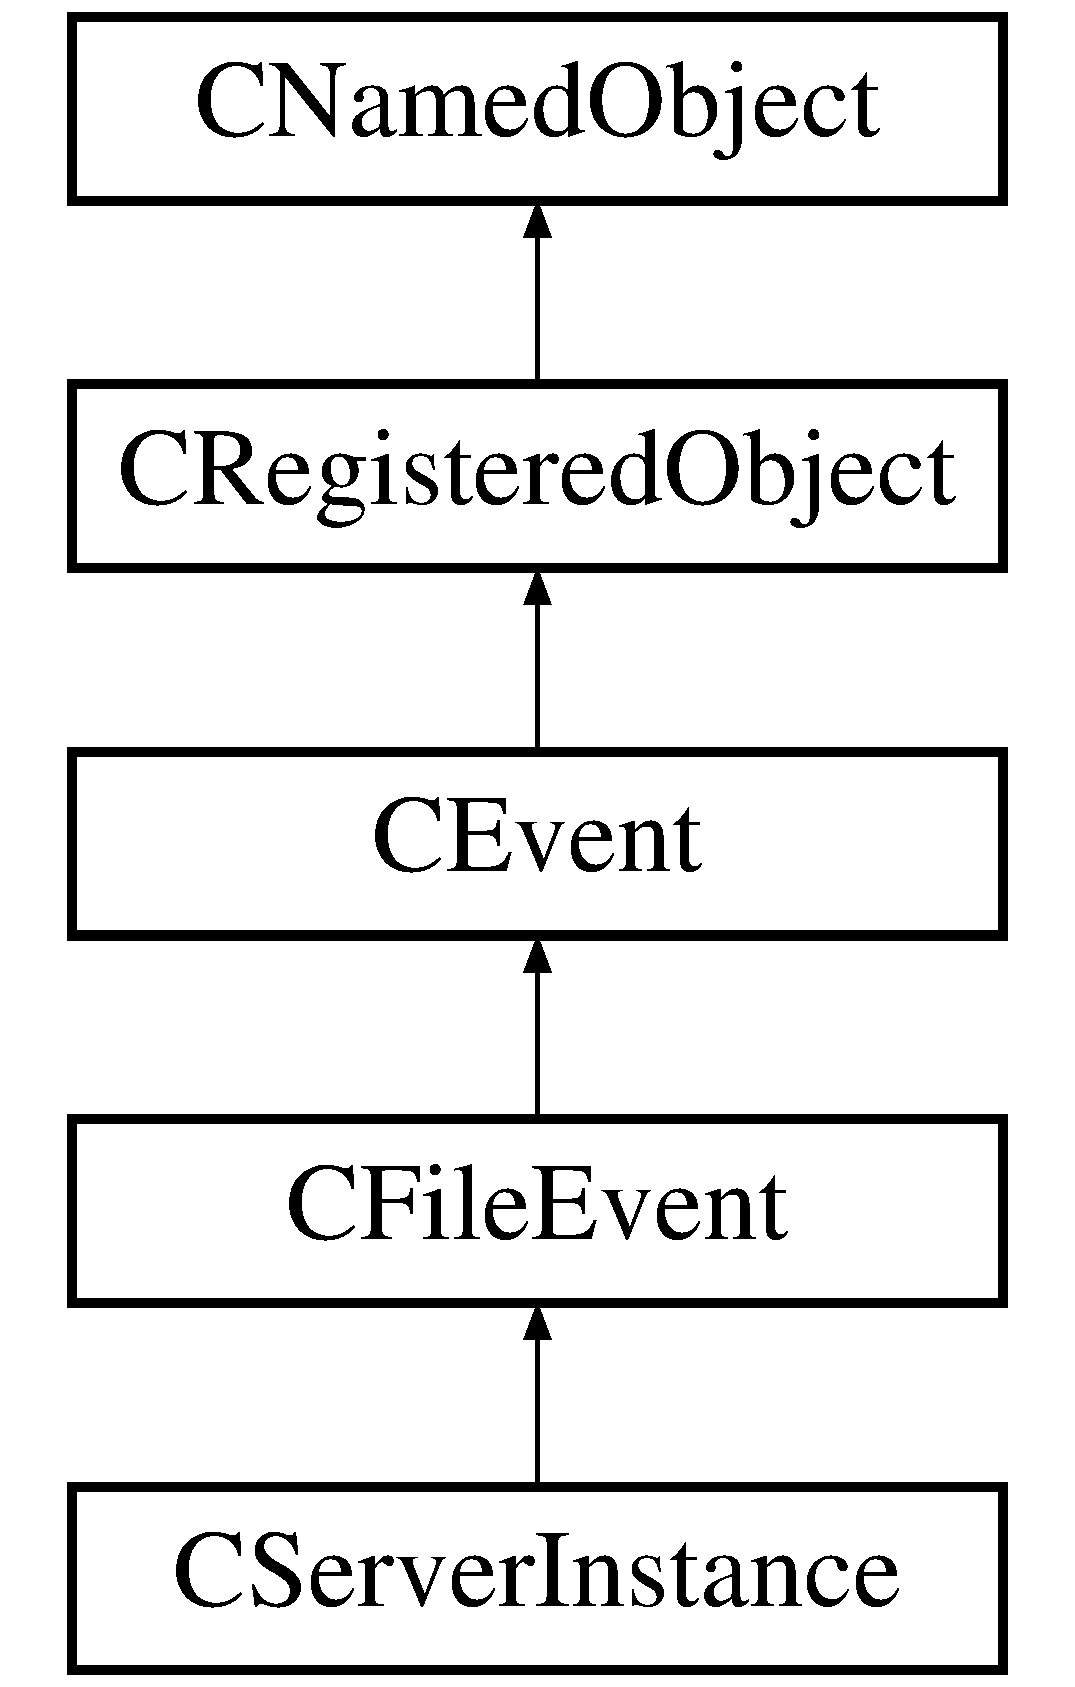
\includegraphics[height=5cm]{classCServerInstance}
\end{center}
\end{figure}
\subsection*{Public Methods}
\begin{CompactItemize}
\item 
{\bf CServer\-Instance} ({\bf CSocket} $\ast$p\-Socket, bool f\-Delete\-Socket=true)
\item 
{\bf CServer\-Instance} (const char $\ast$p\-Name, {\bf CSocket} $\ast$p\-Socket, bool f\-Delete\-Socket=true)
\item 
{\bf CServer\-Instance} (const string \&r\-Name, {\bf CSocket} $\ast$p\-Socket, bool f\-Delete\-Socket=true)
\item 
{\bf $\sim$CServer\-Instance} ()
\item 
{\bf CSocket} $\ast$ {\bf get\-Socket} ()
\item 
bool {\bf get\-Delete\-Flag} () const
\item 
string {\bf get\-Peername} () const
\item 
unsigned short {\bf get\-Peer\-Port} () const
\item 
virtual void {\bf On\-Readable} (istream \&r\-Stream)
\item 
virtual void {\bf On\-Request} ({\bf CSocket} $\ast$p\-Connection)
\item 
void {\bf Shutdown} ()
\item 
virtual string {\bf Describe\-Self} ()
\end{CompactItemize}
\subsection*{Protected Methods}
\begin{CompactItemize}
\item 
void {\bf set\-Socket} ({\bf CSocket} $\ast$sock)
\item 
void {\bf set\-Del\-Flag} (bool flag)
\end{CompactItemize}
\subsection*{Private Methods}
\begin{CompactItemize}
\item 
{\bf CServer\-Instance} (const CServer\-Instance \&rhs)
\item 
CServer\-Instance \& {\bf operator=} (const CServer\-Instance \&rhs)
\item 
int {\bf operator==} (const CServer\-Instance \&rhs)
\end{CompactItemize}
\subsection*{Private Attributes}
\begin{CompactItemize}
\item 
{\bf CSocket} $\ast$ {\bf m\_\-p\-Peer}
\begin{CompactList}\small\item\em Pointer to peer socket.\item\end{CompactList}\item 
bool {\bf m\_\-f\-Delete\-Socket}
\begin{CompactList}\small\item\em True if destructor deletes socket.\item\end{CompactList}\end{CompactItemize}


\subsection{Detailed Description}
Encapsulates the funtionality of a `simple' Tcp/Ip server instance. Simpler tcp/ip server instances are connections with a client over a socket which operate in the simple::\begin{CompactItemize}
\item 
Accept a request from the client.\item 
Respond to those requests mode.\end{CompactItemize}
This class is a subclass of the {\bf CFile\-Event} {\rm (p.\,\pageref{classCFileEvent})} class... On\-Readable is overridden by this class, the user, should in turn override this class and override {\bf On\-Request}() {\rm (p.\,\pageref{classCServerInstance_a9})}. {\bf On\-Request}() {\rm (p.\,\pageref{classCServerInstance_a9})} entered with the application serialization mutex held, and therefore can perform any function which requires global syncrhonization. 



Definition at line 321 of file CServer\-Instance.h.

\subsection{Constructor \& Destructor Documentation}
\index{CServerInstance@{CServer\-Instance}!CServerInstance@{CServerInstance}}
\index{CServerInstance@{CServerInstance}!CServerInstance@{CServer\-Instance}}
\subsubsection{\setlength{\rightskip}{0pt plus 5cm}CServer\-Instance::CServer\-Instance ({\bf CSocket} $\ast$ {\em p\-Socket}, bool {\em f\-Delete\-Socket} = true)}\label{classCServerInstance_a0}


Construct an anonymous server instance:\begin{Desc}
\item[Parameters: ]\par
\begin{description}
\item[{\em 
p\-Socket}]- Pointer to the socket open to the client. \item[{\em 
f\-Delete\-Socket}]- true if the destructor should delete the socket. \end{description}
\end{Desc}


Definition at line 300 of file CServer\-Instance.cpp.\index{CServerInstance@{CServer\-Instance}!CServerInstance@{CServerInstance}}
\index{CServerInstance@{CServerInstance}!CServerInstance@{CServer\-Instance}}
\subsubsection{\setlength{\rightskip}{0pt plus 5cm}CServer\-Instance::CServer\-Instance (const char $\ast$ {\em p\-Name}, {\bf CSocket} $\ast$ {\em p\-Socket}, bool {\em f\-Delete\-Socket} = true)}\label{classCServerInstance_a1}


Construct a server instance whose name comes from a char$\ast$ string.\begin{Desc}
\item[Parameters: ]\par
\begin{description}
\item[{\em 
p\-Name}]- Name to give to the instance (const char$\ast$) [in] \item[{\em 
p\-Socket}]- Socket open on peer. ({\bf CSocket} {\rm (p.\,\pageref{classCSocket})}$\ast$ ) [in] \item[{\em 
f\-Delete\-Socket}]- true to delete sock on destruct (bool) [in = true] \end{description}
\end{Desc}


Definition at line 314 of file CServer\-Instance.cpp.\index{CServerInstance@{CServer\-Instance}!CServerInstance@{CServerInstance}}
\index{CServerInstance@{CServerInstance}!CServerInstance@{CServer\-Instance}}
\subsubsection{\setlength{\rightskip}{0pt plus 5cm}CServer\-Instance::CServer\-Instance (const string \& {\em r\-Name}, {\bf CSocket} $\ast$ {\em p\-Socket}, bool {\em f\-Delete\-Socket} = true)}\label{classCServerInstance_a2}


Construct a server instance whose name comes from a string\& string.\begin{Desc}
\item[Parameters: ]\par
\begin{description}
\item[{\em 
r\-Name}]- Name to give to the instance (const string\& [in]). \item[{\em 
p\-Socket-}]Socket already open on peer ({\bf CSocket} {\rm (p.\,\pageref{classCSocket})}$\ast$ [in]). \item[{\em 
f\-Delete\-Socket}]- true to delete sock on destruction. (bool [in] = true). \end{description}
\end{Desc}


Definition at line 328 of file CServer\-Instance.cpp.\index{CServerInstance@{CServer\-Instance}!~CServerInstance@{$\sim$CServerInstance}}
\index{~CServerInstance@{$\sim$CServerInstance}!CServerInstance@{CServer\-Instance}}
\subsubsection{\setlength{\rightskip}{0pt plus 5cm}CServer\-Instance::$\sim$CServer\-Instance ()}\label{classCServerInstance_a3}


The destructor just deletes m\_\-p\-Peer if m\_\-f\-Delete\-Socket is true. 

Definition at line 338 of file CServer\-Instance.cpp.

References CSocket::Connected, CSocket::get\-State(), m\_\-p\-Peer, and CSocket::Shutdown().\index{CServerInstance@{CServer\-Instance}!CServerInstance@{CServerInstance}}
\index{CServerInstance@{CServerInstance}!CServerInstance@{CServer\-Instance}}
\subsubsection{\setlength{\rightskip}{0pt plus 5cm}CServer\-Instance::CServer\-Instance (const CServer\-Instance \& {\em rhs})\hspace{0.3cm}{\tt  [private]}}\label{classCServerInstance_c0}




\subsection{Member Function Documentation}
\index{CServerInstance@{CServer\-Instance}!DescribeSelf@{DescribeSelf}}
\index{DescribeSelf@{DescribeSelf}!CServerInstance@{CServer\-Instance}}
\subsubsection{\setlength{\rightskip}{0pt plus 5cm}string CServer\-Instance::Describe\-Self ()\hspace{0.3cm}{\tt  [virtual]}}\label{classCServerInstance_a11}


Describe this textually. 

Reimplemented from {\bf CFile\-Event} {\rm (p.\,\pageref{classCFileEvent_a19})}.

Definition at line 447 of file CServer\-Instance.cpp.

References CEvent::Describe\-Self(), CSocket::get\-Socket\-Fd(), CSocket::get\-State(), m\_\-f\-Delete\-Socket, m\_\-p\-Peer, and CSocket::State\-Name().\index{CServerInstance@{CServer\-Instance}!getDeleteFlag@{getDeleteFlag}}
\index{getDeleteFlag@{getDeleteFlag}!CServerInstance@{CServer\-Instance}}
\subsubsection{\setlength{\rightskip}{0pt plus 5cm}bool CServer\-Instance::get\-Delete\-Flag () const\hspace{0.3cm}{\tt  [inline]}}\label{classCServerInstance_a5}




Definition at line 349 of file CServer\-Instance.h.

References m\_\-f\-Delete\-Socket.\index{CServerInstance@{CServer\-Instance}!getPeername@{getPeername}}
\index{getPeername@{getPeername}!CServerInstance@{CServer\-Instance}}
\subsubsection{\setlength{\rightskip}{0pt plus 5cm}string CServer\-Instance::get\-Peername () const}\label{classCServerInstance_a6}


Determines the node to which this socket is connected.\begin{Desc}
\item[Return values: ]\par
\begin{description}
\item[{\em 
string\&}]The name of the peer to which this socket is connected. if the peer has a dns entry the name of the peer is returned, otherwise the IP address is converted to dotted string form and returned. See {\bf CSocket::get\-Peer}() {\rm (p.\,\pageref{classCSocket_a13})}\end{description}
\end{Desc}
\begin{Desc}
\item[Note: ]\par
Can throw any exception thrown by {\bf CSocket::get\-Peer}() {\rm (p.\,\pageref{classCSocket_a13})} \end{Desc}


Definition at line 361 of file CServer\-Instance.cpp.

References CSocket::get\-Peer(), and m\_\-p\-Peer.\index{CServerInstance@{CServer\-Instance}!getPeerPort@{getPeerPort}}
\index{getPeerPort@{getPeerPort}!CServerInstance@{CServer\-Instance}}
\subsubsection{\setlength{\rightskip}{0pt plus 5cm}unsigned short CServer\-Instance::get\-Peer\-Port () const}\label{classCServerInstance_a7}


Determines the port to which the socket is connected on the peer.\begin{Desc}
\item[Return values: ]\par
\begin{description}
\item[{\em 
int}]The port number assigned to this socket.\end{description}
\end{Desc}
\begin{Desc}
\item[Note: ]\par
Can throw any exception thrown by {\bf CSocket::get\-Peer}() {\rm (p.\,\pageref{classCSocket_a13})} \end{Desc}


Definition at line 380 of file CServer\-Instance.cpp.

References CSocket::get\-Peer(), and m\_\-p\-Peer.\index{CServerInstance@{CServer\-Instance}!getSocket@{getSocket}}
\index{getSocket@{getSocket}!CServerInstance@{CServer\-Instance}}
\subsubsection{\setlength{\rightskip}{0pt plus 5cm}{\bf CSocket}$\ast$ CServer\-Instance::get\-Socket ()\hspace{0.3cm}{\tt  [inline]}}\label{classCServerInstance_a4}




Definition at line 346 of file CServer\-Instance.h.\index{CServerInstance@{CServer\-Instance}!OnReadable@{OnReadable}}
\index{OnReadable@{OnReadable}!CServerInstance@{CServer\-Instance}}
\subsubsection{\setlength{\rightskip}{0pt plus 5cm}void CServer\-Instance::On\-Readable (istream \& {\em r\-Input})\hspace{0.3cm}{\tt  [virtual]}}\label{classCServerInstance_a8}


Called when the socket becomes readable. We get the socket and pass that to On\-Request which is what the user is supposed to override and embed application functionality in.\begin{Desc}
\item[Parameters: ]\par
\begin{description}
\item[{\em 
r\-Input}]- Stream open on the socket (istream\& [in-out])\end{description}
\end{Desc}
\begin{Desc}
\item[Note: ]\par
DO NOT OVERRIDE THIS \end{Desc}


Reimplemented from {\bf CFile\-Event} {\rm (p.\,\pageref{classCFileEvent_a15})}.

Definition at line 402 of file CServer\-Instance.cpp.

References m\_\-p\-Peer, On\-Request(), and Shutdown().\index{CServerInstance@{CServer\-Instance}!OnRequest@{OnRequest}}
\index{OnRequest@{OnRequest}!CServerInstance@{CServer\-Instance}}
\subsubsection{\setlength{\rightskip}{0pt plus 5cm}void CServer\-Instance::On\-Request ({\bf CSocket} $\ast$ {\em p\-Connection})\hspace{0.3cm}{\tt  [virtual]}}\label{classCServerInstance_a9}


Called when the client has a request of the server. The application has overridden this member in its derived class.\begin{Desc}
\item[Parameters: ]\par
\begin{description}
\item[{\em 
p\-Connection}]- Socket open to the peer ({\bf CSocket} {\rm (p.\,\pageref{classCSocket})}$\ast$ [in-out]). \end{description}
\end{Desc}


Definition at line 418 of file CServer\-Instance.cpp.

Referenced by On\-Readable().\index{CServerInstance@{CServer\-Instance}!operator=@{operator=}}
\index{operator=@{operator=}!CServerInstance@{CServer\-Instance}}
\subsubsection{\setlength{\rightskip}{0pt plus 5cm}CServer\-Instance\& CServer\-Instance::operator= (const CServer\-Instance \& {\em rhs})\hspace{0.3cm}{\tt  [private]}}\label{classCServerInstance_c1}


\index{CServerInstance@{CServer\-Instance}!operator==@{operator==}}
\index{operator==@{operator==}!CServerInstance@{CServer\-Instance}}
\subsubsection{\setlength{\rightskip}{0pt plus 5cm}int CServer\-Instance::operator== (const CServer\-Instance \& {\em rhs})\hspace{0.3cm}{\tt  [private]}}\label{classCServerInstance_c2}


\index{CServerInstance@{CServer\-Instance}!setDelFlag@{setDelFlag}}
\index{setDelFlag@{setDelFlag}!CServerInstance@{CServer\-Instance}}
\subsubsection{\setlength{\rightskip}{0pt plus 5cm}void CServer\-Instance::set\-Del\-Flag (bool {\em flag})\hspace{0.3cm}{\tt  [inline, protected]}}\label{classCServerInstance_b1}




Definition at line 361 of file CServer\-Instance.h.

References m\_\-f\-Delete\-Socket.\index{CServerInstance@{CServer\-Instance}!setSocket@{setSocket}}
\index{setSocket@{setSocket}!CServerInstance@{CServer\-Instance}}
\subsubsection{\setlength{\rightskip}{0pt plus 5cm}void CServer\-Instance::set\-Socket ({\bf CSocket} $\ast$ {\em sock})\hspace{0.3cm}{\tt  [inline, protected]}}\label{classCServerInstance_b0}




Definition at line 358 of file CServer\-Instance.h.\index{CServerInstance@{CServer\-Instance}!Shutdown@{Shutdown}}
\index{Shutdown@{Shutdown}!CServerInstance@{CServer\-Instance}}
\subsubsection{\setlength{\rightskip}{0pt plus 5cm}void CServer\-Instance::Shutdown ()}\label{classCServerInstance_a10}


Called when we want to shutdown the server we must:\begin{enumerate}
\item 
Remove all fd monitoring.\item 
Clear the enable flag.\item 
Shutdown the socket.\end{enumerate}
It's someone else's responsibility to reap these threads and delete the objects. 

Definition at line 434 of file CServer\-Instance.cpp.

References CSocket::Connected, CSocket::get\-State(), m\_\-p\-Peer, CFile\-Event::Monitor\-Readable(), CEvent::set\-Enable(), and CSocket::Shutdown().

Referenced by On\-Readable().

\subsection{Member Data Documentation}
\index{CServerInstance@{CServer\-Instance}!m_fDeleteSocket@{m\_\-fDeleteSocket}}
\index{m_fDeleteSocket@{m\_\-fDeleteSocket}!CServerInstance@{CServer\-Instance}}
\subsubsection{\setlength{\rightskip}{0pt plus 5cm}bool CServer\-Instance::m\_\-f\-Delete\-Socket\hspace{0.3cm}{\tt  [private]}}\label{classCServerInstance_o1}


True if destructor deletes socket.



Definition at line 325 of file CServer\-Instance.h.

Referenced by Describe\-Self(), get\-Delete\-Flag(), and set\-Del\-Flag().\index{CServerInstance@{CServer\-Instance}!m_pPeer@{m\_\-pPeer}}
\index{m_pPeer@{m\_\-pPeer}!CServerInstance@{CServer\-Instance}}
\subsubsection{\setlength{\rightskip}{0pt plus 5cm}{\bf CSocket}$\ast$ CServer\-Instance::m\_\-p\-Peer\hspace{0.3cm}{\tt  [private]}}\label{classCServerInstance_o0}


Pointer to peer socket.



Definition at line 324 of file CServer\-Instance.h.

Referenced by Describe\-Self(), get\-Peername(), get\-Peer\-Port(), On\-Readable(), Shutdown(), and $\sim$CServer\-Instance().

The documentation for this class was generated from the following files:\begin{CompactItemize}
\item 
{\bf CServer\-Instance.h}\item 
{\bf CServer\-Instance.cpp}\end{CompactItemize}

\section{CServer\-Monitor  Class Reference}
\label{classCServerMonitor}\index{CServerMonitor@{CServer\-Monitor}}
$\backslash$class: CServer\-Monitor $\backslash$file: {\bf CServer\-Monitor.h}. 


{\tt \#include $<$CServer\-Monitor.h$>$}

Inheritance diagram for CServer\-Monitor::\begin{figure}[H]
\begin{center}
\leavevmode
\includegraphics[height=5cm]{classCServerMonitor}
\end{center}
\end{figure}
\subsection*{Public Methods}
\begin{CompactItemize}
\item 
{\bf CServer\-Monitor} ()
\begin{CompactList}\small\item\em Associated Socket.\item\end{CompactList}\item 
{\bf $\sim$CServer\-Monitor} ()
\item 
{\bf CServer\-Monitor} ({\bf CSocket} \&am\_\-Socket)
\item 
{\bf CServer\-Monitor} (const CServer\-Monitor \&a\-CServer\-Monitor)
\item 
CServer\-Monitor \& {\bf operator=} (const CServer\-Monitor \&a\-CServer\-Monitor)
\item 
int {\bf operator==} (const CServer\-Monitor \&a\-CServer\-Monitor) const
\item 
{\bf CSocket} \& {\bf getm\_\-Socket} () const
\item 
void {\bf operator()} ()
\item 
virtual string {\bf Describe\-Self} ()
\end{CompactItemize}
\subsection*{Protected Methods}
\begin{CompactItemize}
\item 
void {\bf setm\_\-Socket} (const {\bf CSocket} \&am\_\-Socket)
\end{CompactItemize}
\subsection*{Private Attributes}
\begin{CompactItemize}
\item 
{\bf CSocket} \& {\bf m\_\-Socket}
\end{CompactItemize}


\subsection{Detailed Description}
$\backslash$class: CServer\-Monitor $\backslash$file: {\bf CServer\-Monitor.h}.

Monitors a TCP/IP socket for connection requests. When a connection request is available, returns. Note that it is up to the reactor to actually accept the connection request. Server\-Monitors can have monitors which are descended from CFd\-Moniitors 



Definition at line 312 of file CServer\-Monitor.h.

\subsection{Constructor \& Destructor Documentation}
\index{CServerMonitor@{CServer\-Monitor}!CServerMonitor@{CServerMonitor}}
\index{CServerMonitor@{CServerMonitor}!CServerMonitor@{CServer\-Monitor}}
\subsubsection{\setlength{\rightskip}{0pt plus 5cm}CServer\-Monitor::CServer\-Monitor ()}\label{classCServerMonitor_a0}


Associated Socket.



Definition at line 301 of file CServer\-Monitor.cpp.\index{CServerMonitor@{CServer\-Monitor}!~CServerMonitor@{$\sim$CServerMonitor}}
\index{~CServerMonitor@{$\sim$CServerMonitor}!CServerMonitor@{CServer\-Monitor}}
\subsubsection{\setlength{\rightskip}{0pt plus 5cm}CServer\-Monitor::$\sim$CServer\-Monitor ()}\label{classCServerMonitor_a1}




Definition at line 312 of file CServer\-Monitor.cpp.\index{CServerMonitor@{CServer\-Monitor}!CServerMonitor@{CServerMonitor}}
\index{CServerMonitor@{CServerMonitor}!CServerMonitor@{CServer\-Monitor}}
\subsubsection{\setlength{\rightskip}{0pt plus 5cm}CServer\-Monitor::CServer\-Monitor ({\bf CSocket} \& {\em am\_\-Socket})}\label{classCServerMonitor_a2}




Definition at line 319 of file CServer\-Monitor.cpp.

References m\_\-Socket.\index{CServerMonitor@{CServer\-Monitor}!CServerMonitor@{CServerMonitor}}
\index{CServerMonitor@{CServerMonitor}!CServerMonitor@{CServer\-Monitor}}
\subsubsection{\setlength{\rightskip}{0pt plus 5cm}CServer\-Monitor::CServer\-Monitor (const CServer\-Monitor \& {\em a\-CServer\-Monitor})}\label{classCServerMonitor_a3}




Definition at line 329 of file CServer\-Monitor.cpp.

References m\_\-Socket.

\subsection{Member Function Documentation}
\index{CServerMonitor@{CServer\-Monitor}!DescribeSelf@{DescribeSelf}}
\index{DescribeSelf@{DescribeSelf}!CServerMonitor@{CServer\-Monitor}}
\subsubsection{\setlength{\rightskip}{0pt plus 5cm}string CServer\-Monitor::Describe\-Self ()\hspace{0.3cm}{\tt  [virtual]}}\label{classCServerMonitor_a8}


Operation Type: selector

Purpose:

Describes self as a file descriptor which has a socket that has a state. 

Reimplemented from {\bf CFd\-Monitor} {\rm (p.\,\pageref{classCFdMonitor_a12})}.

Definition at line 393 of file CServer\-Monitor.cpp.\index{CServerMonitor@{CServer\-Monitor}!getm_Socket@{getm\_\-Socket}}
\index{getm_Socket@{getm\_\-Socket}!CServerMonitor@{CServer\-Monitor}}
\subsubsection{\setlength{\rightskip}{0pt plus 5cm}{\bf CSocket}\& CServer\-Monitor::getm\_\-Socket () const\hspace{0.3cm}{\tt  [inline]}}\label{classCServerMonitor_a6}




Definition at line 360 of file CServer\-Monitor.h.\index{CServerMonitor@{CServer\-Monitor}!operator()@{operator()}}
\index{operator()@{operator()}!CServerMonitor@{CServer\-Monitor}}
\subsubsection{\setlength{\rightskip}{0pt plus 5cm}void CServer\-Monitor::operator() ()\hspace{0.3cm}{\tt  [virtual]}}\label{classCServerMonitor_a7}


Operation Type:

Purpose: 

Reimplemented from {\bf CFd\-Monitor} {\rm (p.\,\pageref{classCFdMonitor_a11})}.

Definition at line 376 of file CServer\-Monitor.cpp.\index{CServerMonitor@{CServer\-Monitor}!operator=@{operator=}}
\index{operator=@{operator=}!CServerMonitor@{CServer\-Monitor}}
\subsubsection{\setlength{\rightskip}{0pt plus 5cm}CServer\-Monitor \& CServer\-Monitor::operator= (const CServer\-Monitor \& {\em a\-CServer\-Monitor})}\label{classCServerMonitor_a4}




Definition at line 339 of file CServer\-Monitor.cpp.

References m\_\-Socket, and CFd\-Monitor::operator=().\index{CServerMonitor@{CServer\-Monitor}!operator==@{operator==}}
\index{operator==@{operator==}!CServerMonitor@{CServer\-Monitor}}
\subsubsection{\setlength{\rightskip}{0pt plus 5cm}int CServer\-Monitor::operator== (const CServer\-Monitor \& {\em a\-CServer\-Monitor}) const}\label{classCServerMonitor_a5}




Definition at line 349 of file CServer\-Monitor.cpp.

References m\_\-Socket, and CFd\-Monitor::operator==().\index{CServerMonitor@{CServer\-Monitor}!setm_Socket@{setm\_\-Socket}}
\index{setm_Socket@{setm\_\-Socket}!CServerMonitor@{CServer\-Monitor}}
\subsubsection{\setlength{\rightskip}{0pt plus 5cm}void CServer\-Monitor::setm\_\-Socket (const {\bf CSocket} \& {\em am\_\-Socket})\hspace{0.3cm}{\tt  [inline, protected]}}\label{classCServerMonitor_b0}




Definition at line 369 of file CServer\-Monitor.h.

\subsection{Member Data Documentation}
\index{CServerMonitor@{CServer\-Monitor}!m_Socket@{m\_\-Socket}}
\index{m_Socket@{m\_\-Socket}!CServerMonitor@{CServer\-Monitor}}
\subsubsection{\setlength{\rightskip}{0pt plus 5cm}{\bf CSocket}\& CServer\-Monitor::m\_\-Socket\hspace{0.3cm}{\tt  [private]}}\label{classCServerMonitor_o0}




Definition at line 317 of file CServer\-Monitor.h.

Referenced by CServer\-Monitor(), operator=(), and operator==().

The documentation for this class was generated from the following files:\begin{CompactItemize}
\item 
{\bf CServer\-Monitor.h}\item 
{\bf CServer\-Monitor.cpp}\end{CompactItemize}

\section{Shell  Class Reference}
\label{classShell}\index{Shell@{Shell}}
{\tt \#include $<$XMShell.h$>$}

Inheritance diagram for Shell::\begin{figure}[H]
\begin{center}
\leavevmode
\includegraphics[height=3cm]{classShell}
\end{center}
\end{figure}
\subsection*{Public Methods}
\begin{CompactItemize}
\item 
{\bf Shell} (String shellname, Widget\-Class shelltype, {\bf XMWidget} $\ast$parent, Arg\-List args=NULL, Cardinal num\_\-args=0)
\item 
{\bf $\sim$Shell} ()
\item 
void {\bf Allow\-Resize} (Boolean allow)
\item 
Boolean {\bf Is\-Resize\-Allowed} ()
\item 
void {\bf Set\-Geometry} (String newg)
\item 
void {\bf Get\-Geometry} (String geom)
\item 
void {\bf Set\-Save\-Under} (Boolean newstate)
\item 
Boolean {\bf Get\-Save\-Under} ()
\item 
void {\bf Realize} ()
\item 
void {\bf Manage} ()
\item 
void {\bf Un\-Manage} ()
\end{CompactItemize}
\subsection*{Protected Attributes}
\begin{CompactItemize}
\item 
{\bf XMCallback}$<$ Shell $>$ {\bf Popdown}
\item 
{\bf XMCallback}$<$ Shell $>$ {\bf Popup}
\end{CompactItemize}
\subsection*{Private Methods}
\begin{CompactItemize}
\item 
virtual void {\bf Popup\-Cb} ({\bf XMWidget} $\ast$shell, Xt\-Pointer user\_\-d, Xt\-Pointer call\_\-d)
\item 
virtual void {\bf Popdn\-Cb} ({\bf XMWidget} $\ast$shell, Xt\-Pointer user\_\-d, Xt\-Pointer call\_\-d)
\end{CompactItemize}


\subsection{Constructor \& Destructor Documentation}
\index{Shell@{Shell}!Shell@{Shell}}
\index{Shell@{Shell}!Shell@{Shell}}
\subsubsection{\setlength{\rightskip}{0pt plus 5cm}Shell::Shell (String {\em shellname}, Widget\-Class {\em shelltype}, {\bf XMWidget} $\ast$ {\em parent}, Arg\-List {\em args} = NULL, Cardinal {\em num\_\-args} = 0)}\label{classShell_a0}




Definition at line 323 of file XMShell.cpp.

References XMWidget::getid(), XMWidget::id, Popdn\-Cb(), Popdown, Popup, Popup\-Cb(), and XMCallback$<$ Shell $>$::Register().\index{Shell@{Shell}!~Shell@{$\sim$Shell}}
\index{~Shell@{$\sim$Shell}!Shell@{Shell}}
\subsubsection{\setlength{\rightskip}{0pt plus 5cm}Shell::$\sim$Shell ()}\label{classShell_a1}




Definition at line 385 of file XMShell.cpp.

References Popdown, Popup, Un\-Manage(), and XMCallback$<$ Shell $>$::Un\-Register().

\subsection{Member Function Documentation}
\index{Shell@{Shell}!AllowResize@{AllowResize}}
\index{AllowResize@{AllowResize}!Shell@{Shell}}
\subsubsection{\setlength{\rightskip}{0pt plus 5cm}void Shell::Allow\-Resize (Boolean {\em allow})\hspace{0.3cm}{\tt  [inline]}}\label{classShell_a2}




Definition at line 311 of file XMShell.h.

References XMWidget::Set\-Attribute().\index{Shell@{Shell}!GetGeometry@{GetGeometry}}
\index{GetGeometry@{GetGeometry}!Shell@{Shell}}
\subsubsection{\setlength{\rightskip}{0pt plus 5cm}void Shell::Get\-Geometry (String {\em geom})\hspace{0.3cm}{\tt  [inline]}}\label{classShell_a5}




Definition at line 322 of file XMShell.h.

References XMWidget::Get\-Attribute().\index{Shell@{Shell}!GetSaveUnder@{GetSaveUnder}}
\index{GetSaveUnder@{GetSaveUnder}!Shell@{Shell}}
\subsubsection{\setlength{\rightskip}{0pt plus 5cm}Boolean Shell::Get\-Save\-Under ()\hspace{0.3cm}{\tt  [inline]}}\label{classShell_a7}




Definition at line 327 of file XMShell.h.

References XMWidget::Get\-Attribute().\index{Shell@{Shell}!IsResizeAllowed@{IsResizeAllowed}}
\index{IsResizeAllowed@{IsResizeAllowed}!Shell@{Shell}}
\subsubsection{\setlength{\rightskip}{0pt plus 5cm}Boolean Shell::Is\-Resize\-Allowed ()\hspace{0.3cm}{\tt  [inline]}}\label{classShell_a3}




Definition at line 313 of file XMShell.h.

References XMWidget::Get\-Attribute().\index{Shell@{Shell}!Manage@{Manage}}
\index{Manage@{Manage}!Shell@{Shell}}
\subsubsection{\setlength{\rightskip}{0pt plus 5cm}void Shell::Manage ()\hspace{0.3cm}{\tt  [inline]}}\label{classShell_a9}




Reimplemented from {\bf XMWidget} {\rm (p.\,\pageref{classXMWidget_a16})}.

Definition at line 339 of file XMShell.h.

References XMWidget::id.

Referenced by Realize().\index{Shell@{Shell}!PopdnCb@{PopdnCb}}
\index{PopdnCb@{PopdnCb}!Shell@{Shell}}
\subsubsection{\setlength{\rightskip}{0pt plus 5cm}void Shell::Popdn\-Cb ({\bf XMWidget} $\ast$ {\em shell}, Xt\-Pointer {\em user\_\-d}, Xt\-Pointer {\em call\_\-d})\hspace{0.3cm}{\tt  [private, virtual]}}\label{classShell_c1}




Definition at line 402 of file XMShell.cpp.

Referenced by Shell().\index{Shell@{Shell}!PopupCb@{PopupCb}}
\index{PopupCb@{PopupCb}!Shell@{Shell}}
\subsubsection{\setlength{\rightskip}{0pt plus 5cm}void Shell::Popup\-Cb ({\bf XMWidget} $\ast$ {\em shell}, Xt\-Pointer {\em user\_\-d}, Xt\-Pointer {\em call\_\-d})\hspace{0.3cm}{\tt  [private, virtual]}}\label{classShell_c0}




Definition at line 399 of file XMShell.cpp.

Referenced by Shell().\index{Shell@{Shell}!Realize@{Realize}}
\index{Realize@{Realize}!Shell@{Shell}}
\subsubsection{\setlength{\rightskip}{0pt plus 5cm}void Shell::Realize ()\hspace{0.3cm}{\tt  [inline]}}\label{classShell_a8}




Reimplemented from {\bf XMWidget} {\rm (p.\,\pageref{classXMWidget_a18})}.

Definition at line 334 of file XMShell.h.

References XMWidget::id, and Manage().\index{Shell@{Shell}!SetGeometry@{SetGeometry}}
\index{SetGeometry@{SetGeometry}!Shell@{Shell}}
\subsubsection{\setlength{\rightskip}{0pt plus 5cm}void Shell::Set\-Geometry (String {\em newg})\hspace{0.3cm}{\tt  [inline]}}\label{classShell_a4}




Definition at line 320 of file XMShell.h.

References XMWidget::Set\-Attribute().\index{Shell@{Shell}!SetSaveUnder@{SetSaveUnder}}
\index{SetSaveUnder@{SetSaveUnder}!Shell@{Shell}}
\subsubsection{\setlength{\rightskip}{0pt plus 5cm}void Shell::Set\-Save\-Under (Boolean {\em newstate})\hspace{0.3cm}{\tt  [inline]}}\label{classShell_a6}




Definition at line 325 of file XMShell.h.

References XMWidget::Set\-Attribute().\index{Shell@{Shell}!UnManage@{UnManage}}
\index{UnManage@{UnManage}!Shell@{Shell}}
\subsubsection{\setlength{\rightskip}{0pt plus 5cm}void Shell::Un\-Manage ()\hspace{0.3cm}{\tt  [inline]}}\label{classShell_a10}




Reimplemented from {\bf XMWidget} {\rm (p.\,\pageref{classXMWidget_a17})}.

Definition at line 340 of file XMShell.h.

References XMWidget::id.

Referenced by $\sim$Shell().

\subsection{Member Data Documentation}
\index{Shell@{Shell}!Popdown@{Popdown}}
\index{Popdown@{Popdown}!Shell@{Shell}}
\subsubsection{\setlength{\rightskip}{0pt plus 5cm}{\bf XMCallback}$<$Shell$>$ Shell::Popdown\hspace{0.3cm}{\tt  [protected]}}\label{classShell_n0}




Definition at line 342 of file XMShell.h.

Referenced by Shell(), and $\sim$Shell().\index{Shell@{Shell}!Popup@{Popup}}
\index{Popup@{Popup}!Shell@{Shell}}
\subsubsection{\setlength{\rightskip}{0pt plus 5cm}{\bf XMCallback}$<$Shell$>$ Shell::Popup\hspace{0.3cm}{\tt  [protected]}}\label{classShell_n1}




Definition at line 343 of file XMShell.h.

Referenced by Shell(), and $\sim$Shell().

The documentation for this class was generated from the following files:\begin{CompactItemize}
\item 
{\bf XMShell.h}\item 
{\bf XMShell.cpp}\end{CompactItemize}

\section{CShutdown\-Binding  Class Reference}
\label{classCShutdownBinding}\index{CShutdownBinding@{CShutdown\-Binding}}
\subsection*{Public Methods}
\begin{CompactItemize}
\item 
{\bf CShutdown\-Binding} ({\bf CTCLInterpreter} \&r\-Interp)
\item 
void {\bf operator()} ({\bf CType\-Free\-Binding} $\ast$p\-Binding)
\end{CompactItemize}
\subsection*{Private Attributes}
\begin{CompactItemize}
\item 
{\bf CTCLInterpreter} \& {\bf m\_\-r\-Interp}
\end{CompactItemize}


\subsection{Constructor \& Destructor Documentation}
\index{CShutdownBinding@{CShutdown\-Binding}!CShutdownBinding@{CShutdownBinding}}
\index{CShutdownBinding@{CShutdownBinding}!CShutdownBinding@{CShutdown\-Binding}}
\subsubsection{\setlength{\rightskip}{0pt plus 5cm}CShutdown\-Binding::CShutdown\-Binding ({\bf CTCLInterpreter} \& {\em r\-Interp})\hspace{0.3cm}{\tt  [inline]}}\label{classCShutdownBinding_a0}




Definition at line 329 of file CConfiguration\-Manager.cpp.

\subsection{Member Function Documentation}
\index{CShutdownBinding@{CShutdown\-Binding}!operator()@{operator()}}
\index{operator()@{operator()}!CShutdownBinding@{CShutdown\-Binding}}
\subsubsection{\setlength{\rightskip}{0pt plus 5cm}void CShutdown\-Binding::operator() ({\bf CType\-Free\-Binding} $\ast$ {\em p\-Binding})\hspace{0.3cm}{\tt  [inline]}}\label{classCShutdownBinding_a1}




Definition at line 330 of file CConfiguration\-Manager.cpp.

References CType\-Free\-Binding::Shutdown\-Bindings().

\subsection{Member Data Documentation}
\index{CShutdownBinding@{CShutdown\-Binding}!m_rInterp@{m\_\-rInterp}}
\index{m_rInterp@{m\_\-rInterp}!CShutdownBinding@{CShutdown\-Binding}}
\subsubsection{\setlength{\rightskip}{0pt plus 5cm}{\bf CTCLInterpreter}\& CShutdown\-Binding::m\_\-r\-Interp\hspace{0.3cm}{\tt  [private]}}\label{classCShutdownBinding_o0}




Definition at line 327 of file CConfiguration\-Manager.cpp.

The documentation for this class was generated from the following file:\begin{CompactItemize}
\item 
{\bf CConfiguration\-Manager.cpp}\end{CompactItemize}

\section{CSocket  Class Reference}
\label{classCSocket}\index{CSocket@{CSocket}}
{\tt \#include $<$CSocket.h$>$}

\subsection*{Public Types}
\begin{CompactItemize}
\item 
enum {\bf State} \{ {\bf Disconnected}, 
{\bf Bound}, 
{\bf Listening}, 
{\bf Connected}
 \}
\begin{CompactList}\small\item\em Captures the state of the socket. See general remarks for more info.\item\end{CompactList}\end{CompactItemize}
\subsection*{Public Methods}
\begin{CompactItemize}
\item 
{\bf CSocket} ()
\item 
{\bf CSocket} (int am\_\-Fd, {\bf CSocket::State} am\_\-State)
\item 
virtual {\bf $\sim$CSocket} ()
\item 
int {\bf get\-Socket\-Fd} () const
\begin{CompactList}\small\item\em Get accessor function socket file descriptor.\item\end{CompactList}\item 
{\bf CSocket::State} {\bf get\-State} () const
\begin{CompactList}\small\item\em Get accessor function for socket state.\item\end{CompactList}\item 
void {\bf Connect} (const string \&host, const string \&service)
\item 
void {\bf Connect} (unsigned long int Ip\-Address, unsigned short service)
\item 
void {\bf Bind} (const string \&service)
\item 
void {\bf Listen} (unsigned int n\-Backlog=5)
\item 
CSocket $\ast$ {\bf Accept} (string \&client)
\item 
void {\bf Shutdown} ()
\item 
int {\bf Read} (void $\ast$p\-Buffer, size\_\-t n\-Bytes)
\item 
int {\bf Write} (void $\ast$p\-Buffer, size\_\-t n\-Bytes)
\item 
void {\bf get\-Peer} (unsigned short \&port, string \&peer)
\item 
void {\bf OOBInline} (bool {\bf State}=TRUE)
\item 
bool {\bf is\-OOBInline} ()
\item 
void {\bf set\-Rcv\-Low\-Water\-Mark} (size\_\-t n\-Bytes)
\item 
size\_\-t {\bf get\-Rcv\-Low\-Water\-Mark} ()
\item 
void {\bf set\-Snd\-Low\-Water\-Mark} (size\_\-t n\-Bytes)
\item 
size\_\-t {\bf get\-Snd\-Low\-Water\-Mark} ()
\item 
void {\bf set\-Rcv\-Timeout} (unsigned int n\-Ms)
\item 
unsigned int {\bf get\-Rcv\-Timeout} ()
\item 
void {\bf set\-Snd\-Timeout} (unsigned int n\-Ms)
\item 
unsigned int {\bf get\-Snd\-Timeout} ()
\item 
void {\bf Debug} (bool f\-State=TRUE)
\item 
bool {\bf is\-Debug} ()
\item 
void {\bf Set\-Not\-Routable} (bool f\-Routable=TRUE)
\item 
bool {\bf is\-Not\-Routable} ()
\item 
void {\bf set\-Snd\-Buf\-Size} (size\_\-t n\-Buffer\-Size)
\item 
size\_\-t {\bf get\-Snd\-Buf\-Size} ()
\item 
void {\bf set\-Rcv\-Buf\-Size} (size\_\-t n\-Bytes)
\item 
size\_\-t {\bf get\-Rcv\-Buf\-Size} ()
\item 
void {\bf set\-Linger} (bool l\-On, int n\-Linger\-Seconds)
\item 
void {\bf get\-Linger} (bool \&is\-Lingering, int \&n\-Linger\-Seconds)
\end{CompactItemize}
\subsection*{Static Public Methods}
\begin{CompactItemize}
\item 
string {\bf State\-Name} ({\bf CSocket::State} state)
\end{CompactItemize}
\subsection*{Protected Methods}
\begin{CompactItemize}
\item 
void {\bf set\-Socket\-Fd} (const int am\_\-Fd)
\begin{CompactList}\small\item\em Set accessor function for Socket file descriptor.\item\end{CompactList}\item 
void {\bf set\-State} (const {\bf CSocket::State} am\_\-State)
\begin{CompactList}\small\item\em Set accessor function for current socket state.\item\end{CompactList}\item 
unsigned short {\bf Service} (const string \&r\-Service)
\item 
string {\bf Address\-To\-Host\-String} (in\_\-addr peer)
\item 
void {\bf Open\-Socket} ()
\end{CompactItemize}
\subsection*{Static Protected Methods}
\begin{CompactItemize}
\item 
void {\bf Stock\-State\-Map} ()
\end{CompactItemize}
\subsection*{Private Methods}
\begin{CompactItemize}
\item 
{\bf CSocket} (const CSocket \&a\-CSocket)
\begin{CompactList}\small\item\em Copy Constructor forbidden.\item\end{CompactList}\item 
CSocket \& {\bf operator=} (const CSocket \&a\-CSocket)
\begin{CompactList}\small\item\em Assignment Operator Forbidden.\item\end{CompactList}\item 
int {\bf operator==} (const CSocket \&a\-CSocket) const
\begin{CompactList}\small\item\em Equality Operator Forbidden.\item\end{CompactList}\end{CompactItemize}
\subsection*{Private Attributes}
\begin{CompactItemize}
\item 
int {\bf m\_\-Fd}
\begin{CompactList}\small\item\em Socket.\item\end{CompactList}\item 
{\bf CSocket::State} {\bf m\_\-State}
\begin{CompactList}\small\item\em State of socket.\item\end{CompactList}\end{CompactItemize}
\subsection*{Static Private Attributes}
\begin{CompactItemize}
\item 
map$<$ {\bf CSocket::State}, string $>$ {\bf m\_\-State\-Names}
\begin{CompactList}\small\item\em State name lookup tbl.\item\end{CompactList}\end{CompactItemize}


\subsection{Detailed Description}
Encapsulates a generalized TCP/IP SOCK\_\-STREAM socket.  Note that TCP/IP Sockets can come in two flavors: Clients and Servers. Clients must perform a connect, while servers perform a bind, listen and then serveral accepts to create 'server instances'. The state of a socket is maintained in the m\_\-State variable and is from the enumerator: {\bf CSocket::State} {\rm (p.\,\pageref{classCSocket_s4})}

\begin{CompactItemize}
\item 
Disconnected: The socket is not connected to anything.\item 
Bound: The socket is a server socket which is not connected, but has been bound to a service port.\item 
Listening: The socket is a server port which is listening and can therefore accept connections\item 
Connected The socket is either a client or a  server instance and is connected to it's counterpart. \end{CompactItemize}




Definition at line 338 of file CSocket.h.

\subsection{Member Enumeration Documentation}
\index{CSocket@{CSocket}!State@{State}}
\index{State@{State}!CSocket@{CSocket}}
\subsubsection{\setlength{\rightskip}{0pt plus 5cm}enum CSocket::State}\label{classCSocket_s4}


Captures the state of the socket. See general remarks for more info.

\begin{Desc}
\item[Enumeration values:]\par
\begin{description}
\index{Disconnected@{Disconnected}!CSocket@{CSocket}}\index{CSocket@{CSocket}!Disconnected@{Disconnected}}\item[{\em 
{\em Disconnected}\label{classCSocket_s4s0}
}]\index{Bound@{Bound}!CSocket@{CSocket}}\index{CSocket@{CSocket}!Bound@{Bound}}\item[{\em 
{\em Bound}\label{classCSocket_s4s1}
}]\index{Listening@{Listening}!CSocket@{CSocket}}\index{CSocket@{CSocket}!Listening@{Listening}}\item[{\em 
{\em Listening}\label{classCSocket_s4s2}
}]\index{Connected@{Connected}!CSocket@{CSocket}}\index{CSocket@{CSocket}!Connected@{Connected}}\item[{\em 
{\em Connected}\label{classCSocket_s4s3}
}]\end{description}
\end{Desc}



Definition at line 343 of file CSocket.h.

Referenced by CSocket(), CTCPBad\-Socket\-State::CTCPBad\-Socket\-State(), CTCPBad\-Socket\-State::get\-Bad\-State(), get\-State(), OOBInline(), CTCPBad\-Socket\-State::set\-Bad\-State(), set\-State(), and State\-Name().

\subsection{Constructor \& Destructor Documentation}
\index{CSocket@{CSocket}!CSocket@{CSocket}}
\index{CSocket@{CSocket}!CSocket@{CSocket}}
\subsubsection{\setlength{\rightskip}{0pt plus 5cm}CSocket::CSocket ()}\label{classCSocket_a0}


The default constructor initializes the fd to an illegal value and sets the state to Disconnected.  The body of the constructor attempts to set the m\_\-Fd member via a call to  socket(2) to create an INET domain SOCK\_\-STREAM, protocl tcp.

It is up to the user to call Connect or alternatively set up the socket as a server by binding and listening.

Exceptions:

\begin{CompactItemize}
\item 
{\bf CErrno\-Exception} {\rm (p.\,\pageref{classCErrnoException})} if getprotoent for tcp fails or if the socket call itself fails. \end{CompactItemize}


Definition at line 365 of file CSocket.cpp.

References Open\-Socket().

Referenced by Accept().\index{CSocket@{CSocket}!CSocket@{CSocket}}
\index{CSocket@{CSocket}!CSocket@{CSocket}}
\subsubsection{\setlength{\rightskip}{0pt plus 5cm}CSocket::CSocket (int {\em am\_\-Fd}, {\bf CSocket::State} {\em am\_\-State})}\label{classCSocket_a1}


This parameterized constructor is intended to allow a program which already has created a socket in some arbitrary state to wrap it inside a CSocket object. It must be used with care.. in the sense that the am\_\-State parameter must match the actual socket state.\begin{Desc}
\item[Parameters: ]\par
\begin{description}
\item[{\em 
am\_\-Fd}]The file descriptor already open on a socket. \item[{\em 
am\_\-State}]The current state of the socket am\_\-Fd \end{description}
\end{Desc}


Definition at line 398 of file CSocket.cpp.

References State, and Stock\-State\-Map().\index{CSocket@{CSocket}!~CSocket@{$\sim$CSocket}}
\index{~CSocket@{$\sim$CSocket}!CSocket@{CSocket}}
\subsubsection{\setlength{\rightskip}{0pt plus 5cm}CSocket::$\sim$CSocket ()\hspace{0.3cm}{\tt  [virtual]}}\label{classCSocket_a2}


Destructor action depends on the state: sockets which are Connected are shutdown and then closed. Sockets which are in other states are just closed if the fd $>$ 0. 

Definition at line 378 of file CSocket.cpp.\index{CSocket@{CSocket}!CSocket@{CSocket}}
\index{CSocket@{CSocket}!CSocket@{CSocket}}
\subsubsection{\setlength{\rightskip}{0pt plus 5cm}CSocket::CSocket (const CSocket \& {\em a\-CSocket})\hspace{0.3cm}{\tt  [private]}}\label{classCSocket_c0}


Copy Constructor forbidden.



\subsection{Member Function Documentation}
\index{CSocket@{CSocket}!Accept@{Accept}}
\index{Accept@{Accept}!CSocket@{CSocket}}
\subsubsection{\setlength{\rightskip}{0pt plus 5cm}CSocket $\ast$ CSocket::Accept (string \& {\em client})}\label{classCSocket_a9}


This member function can be called on  a server socket. The calling thread is blocked until a connection request is received. At that time, the connection is accepted (granted), and a new CSocket is created in the Connected state. The new CSocket represents a Server Instance socket, communication along that socket can take place immediately and will represent communication with the client.

Exceptions which can be thrown:

\begin{CompactItemize}
\item 
{\bf CTCPBad\-Socket\-State} {\rm (p.\,\pageref{classCTCPBadSocketState})} m\_\-State != Listening\item 
{\bf CErrno\-Exception} {\rm (p.\,\pageref{classCErrnoException})} accept(2) call failed.\end{CompactItemize}
Side effects:

The client parameter is  written with a string representing the hostname of the client or the IP address if the hostname can not be determined.

The socket created is created via new, therefore  it is the responsibility of the caller to delete it.\begin{Desc}
\item[Parameters: ]\par
\begin{description}
\item[{\em 
client}]Recieves the IP information of the connecting host. Where possible, this is the hostname. Where not, a dotted IP address. \end{description}
\end{Desc}


Definition at line 659 of file CSocket.cpp.

References Address\-To\-Host\-String(), Connected, CSocket(), Listening, m\_\-Fd, and m\_\-State.

Referenced by CServer\-Connection\-Event::On\-Readable().\index{CSocket@{CSocket}!AddressToHostString@{AddressToHostString}}
\index{AddressToHostString@{AddressToHostString}!CSocket@{CSocket}}
\subsubsection{\setlength{\rightskip}{0pt plus 5cm}string CSocket::Address\-To\-Host\-String (in\_\-addr {\em peer})\hspace{0.3cm}{\tt  [protected]}}\label{classCSocket_b3}


Purpose: Given an IP address in in\_\-addr format, returns a string describing the address. First gethostbyaddr(3) is used to attempt to get the primary DNS name of the address. If this fails, then inet\_\-ntoa(3) is called to get a dotted string. Note that this entire function must run syncrhonized to the global application mutex since the (3) network database calls are assumed to be nonthreadsafe.\begin{Desc}
\item[Parameters: ]\par
\begin{description}
\item[{\em 
peer}]- The network address of a host in in\_\-addr, network byte order form. \end{description}
\end{Desc}


Definition at line 1503 of file CSocket.cpp.

References CApplication\-Serializer::get\-Instance(), CThread\-Recursive\-Mutex::Lock(), and CThread\-Recursive\-Mutex::Un\-Lock().

Referenced by Accept(), and get\-Peer().\index{CSocket@{CSocket}!Bind@{Bind}}
\index{Bind@{Bind}!CSocket@{CSocket}}
\subsubsection{\setlength{\rightskip}{0pt plus 5cm}void CSocket::Bind (const string \& {\em service})}\label{classCSocket_a7}


Indicates that the socket will be used as a server listener socket, and binds it to a service port. The service can be provided either as a numerical string or as a string translated via getservbyname().

The following exceptions can be thrown:

\begin{CompactItemize}
\item 
{\bf CTCPBad\-Socket\-State} {\rm (p.\,\pageref{classCTCPBadSocketState})} m\_\-State != Disconnected\item 
{\bf CTCPNo\-Such\-Service} {\rm (p.\,\pageref{classCTCPNoSuchService})} Service could not be determined.\item 
{\bf CErrno\-Exception} {\rm (p.\,\pageref{classCErrnoException})} bind(2) failed.\end{CompactItemize}
On success, m\_\-State = Bound 

Definition at line 562 of file CSocket.cpp.

References Bound, Disconnected, m\_\-Fd, m\_\-State, and Service().

Referenced by CServer\-Connection\-Event::Configure\-Socket().\index{CSocket@{CSocket}!Connect@{Connect}}
\index{Connect@{Connect}!CSocket@{CSocket}}
\subsubsection{\setlength{\rightskip}{0pt plus 5cm}void CSocket::Connect (unsigned long int {\em Ip\-Address}, unsigned short {\em service})}\label{classCSocket_a6}


Connects a socket as a client given numerical host, and port numbers in  host byte order. For the host that means that an ip address of form:

aa.bb.cc.dd is stored Hi-$>$Low as aabbccdd in a longword.

See {\bf Connect}(const string\&host, const string\& service) {\rm (p.\,\pageref{classCSocket_a5})} for more information.\begin{Desc}
\item[Parameters: ]\par
\begin{description}
\item[{\em 
Ip\-Address}]The numerical ip address of the server in host byte order. \item[{\em 
service}]The port number of the service. \end{description}
\end{Desc}


Definition at line 495 of file CSocket.cpp.

References Connected, Disconnected, CApplication\-Serializer::get\-Instance(), CThread\-Recursive\-Mutex::Lock(), m\_\-Fd, m\_\-State, and CThread\-Recursive\-Mutex::Un\-Lock().\index{CSocket@{CSocket}!Connect@{Connect}}
\index{Connect@{Connect}!CSocket@{CSocket}}
\subsubsection{\setlength{\rightskip}{0pt plus 5cm}void CSocket::Connect (const string \& {\em host}, const string \& {\em service})}\label{classCSocket_a5}


Operation Type: Connection Control

Indicates that the socket will be used as a client socket and attempts to connect it to a server.  The address of the server can be passed in either in IP address or IP name textual format. Similarly, the port can be passed in as a textual port name (in /etc/services) or a port number.

The action of this function is to convert (if possible) the Host and service  into numeric equivalents and call the overloaded Connect(int Ip\-Address, int service)

Exceptions which can be thrown:

\begin{CompactItemize}
\item 
{\bf CTCPBad\-Socket\-State} {\rm (p.\,\pageref{classCTCPBadSocketState})} -- m\_\-State was not Disconnected\item 
{\bf CTCPNo\-Such\-Host} {\rm (p.\,\pageref{classCTCPNoSuchHost})} - Host not in DNS or nonexistent.\item 
{\bf CTCPNo\-Such\-Service} {\rm (p.\,\pageref{classCTCPNoSuchService})} - Named service does not translate.\item 
{\bf CTCPConnection\-Failed} {\rm (p.\,\pageref{classCTCPConnectionFailed})}- Connection refused by remote host (from Connect(int Ip\-Address, int service).\end{CompactItemize}
\begin{Desc}
\item[Parameters: ]\par
\begin{description}
\item[{\em 
host}]Specifies the system to connect to. This can be either a DNS textual name or a string in dotted IP address format. \item[{\em 
service}]Specifies a service offered by the host. This can be either a service name or the textual equivalent of a service number.\end{description}
\end{Desc}
On Success the socket state is set to Connected. 

Definition at line 443 of file CSocket.cpp.

References Disconnected, CApplication\-Serializer::get\-Instance(), CThread\-Recursive\-Mutex::Lock(), m\_\-State, Service(), and CThread\-Recursive\-Mutex::Un\-Lock().

Referenced by CLogger::Log(), and CAlarm\-Logger::Log().\index{CSocket@{CSocket}!Debug@{Debug}}
\index{Debug@{Debug}!CSocket@{CSocket}}
\subsubsection{\setlength{\rightskip}{0pt plus 5cm}void CSocket::Debug (bool {\em f\-State} = TRUE)}\label{classCSocket_a24}


Purpose:

Attempts to turn on Socket debugging. To support this. The user must have effective UID = 0. .

Throws:\begin{CompactItemize}
\item 
{\bf CErrno\-Exception} {\rm (p.\,\pageref{classCErrnoException})} if an error was returned from setsockopt(2) At present we don't know of systems which don't implement this so all errors will throw.\end{CompactItemize}
\begin{Desc}
\item[Parameters: ]\par
\begin{description}
\item[{\em 
f\-State}][TRUE] Desired state of debugging. TRUE will cause debugging to be turned on. FALSE turned off. \end{description}
\end{Desc}


Definition at line 1193 of file CSocket.cpp.

References m\_\-Fd, and TRUE.\index{CSocket@{CSocket}!getLinger@{getLinger}}
\index{getLinger@{getLinger}!CSocket@{CSocket}}
\subsubsection{\setlength{\rightskip}{0pt plus 5cm}void CSocket::get\-Linger (bool \& {\em is\-Lingering}, int \& {\em n\-Linger\-Seconds})}\label{classCSocket_a33}


Purpose:

Retrieve the linger parameters.

Throws:\begin{CompactItemize}
\item 
{\bf CErrno\-Exception} {\rm (p.\,\pageref{classCErrnoException})} if the setsockopt(2) call failed.\end{CompactItemize}
\begin{Desc}
\item[Parameters: ]\par
\begin{description}
\item[{\em 
is\-Lingering}][out] Receives the value of the linger state:\begin{CompactItemize}
\item 
TRUE linger is enabled.\item 
FALSE linger is not enabled. \end{CompactItemize}
\end{description}
\end{Desc}
\begin{Desc}
\item[Parameters: ]\par
\begin{description}
\item[{\em 
n\-Linger\-Seconds}][out] Receives the value of the linger timeout. This only has meaning in the event that is\-Lingering == TRUE. \end{description}
\end{Desc}


Definition at line 1441 of file CSocket.cpp.

References m\_\-Fd.\index{CSocket@{CSocket}!getPeer@{getPeer}}
\index{getPeer@{getPeer}!CSocket@{CSocket}}
\subsubsection{\setlength{\rightskip}{0pt plus 5cm}void CSocket::get\-Peer (unsigned short \& {\em port}, string \& {\em peer})}\label{classCSocket_a13}


Purpose:

Returns information about who a socket is connected to. If the socket is not connected, {\bf CTCPBad\-Socket\-State} {\rm (p.\,\pageref{classCTCPBadSocketState})} is thrown. If possible, the peername parameter is returned as a string containing the DNS name of the peer. If the DNS lookup fails, the IP address is converted into dotted form.\begin{Desc}
\item[Parameters: ]\par
\begin{description}
\item[{\em 
port}]The number of the port to which the socket is connected. \item[{\em 
peer}]The peer as either a DNS hostname or a dotted IP address.\end{description}
\end{Desc}
Throws:\begin{CompactItemize}
\item 
{\bf CTCPBad\-Socket\-State} {\rm (p.\,\pageref{classCTCPBadSocketState})} if m\_\-State != Connected\item 
{\bf CErrno\-Exception} {\rm (p.\,\pageref{classCErrnoException})} if getpeeername(2) failed. \end{CompactItemize}


Definition at line 870 of file CSocket.cpp.

References Address\-To\-Host\-String(), Connected, m\_\-Fd, and m\_\-State.

Referenced by CServer\-Instance::get\-Peername(), and CServer\-Instance::get\-Peer\-Port().\index{CSocket@{CSocket}!getRcvBufSize@{getRcvBufSize}}
\index{getRcvBufSize@{getRcvBufSize}!CSocket@{CSocket}}
\subsubsection{\setlength{\rightskip}{0pt plus 5cm}size\_\-t CSocket::get\-Rcv\-Buf\-Size ()}\label{classCSocket_a31}


Purpose:

Returns the maximum number of bytes which can be  recieved in a single read(2) call.

Throws:\begin{CompactItemize}
\item 
{\bf CErrno\-Exception} {\rm (p.\,\pageref{classCErrnoException})} if getsockopt(2) fails. \end{CompactItemize}


Definition at line 1375 of file CSocket.cpp.

References m\_\-Fd.\index{CSocket@{CSocket}!getRcvLowWaterMark@{getRcvLowWaterMark}}
\index{getRcvLowWaterMark@{getRcvLowWaterMark}!CSocket@{CSocket}}
\subsubsection{\setlength{\rightskip}{0pt plus 5cm}size\_\-t CSocket::get\-Rcv\-Low\-Water\-Mark ()}\label{classCSocket_a17}


Returns the size of the current receive low water mark. See set\-Rcv\-Low\-Water\-Mark for information about what this parameter does. Note that the value returned is inquired from the socket rather than stored in internal state.

Throws:\begin{CompactItemize}
\item 
{\bf CErrno\-Exception} {\rm (p.\,\pageref{classCErrnoException})} if an error from getsockopt is detected. \end{CompactItemize}


Definition at line 997 of file CSocket.cpp.

References m\_\-Fd.\index{CSocket@{CSocket}!getRcvTimeout@{getRcvTimeout}}
\index{getRcvTimeout@{getRcvTimeout}!CSocket@{CSocket}}
\subsubsection{\setlength{\rightskip}{0pt plus 5cm}unsigned int CSocket::get\-Rcv\-Timeout ()}\label{classCSocket_a21}


Purpose:

Retrieve the protocol receive timeout. The time out is returned as an integer number of milliseconds.

Throws:\begin{CompactItemize}
\item 
{\bf CErrno\-Exception} {\rm (p.\,\pageref{classCErrnoException})} if getsockopt(3) returns an error. \end{CompactItemize}


Definition at line 1098 of file CSocket.cpp.

References m\_\-Fd.\index{CSocket@{CSocket}!getSndBufSize@{getSndBufSize}}
\index{getSndBufSize@{getSndBufSize}!CSocket@{CSocket}}
\subsubsection{\setlength{\rightskip}{0pt plus 5cm}size\_\-t CSocket::get\-Snd\-Buf\-Size ()}\label{classCSocket_a29}


Purpose:

Returns the number of bytes that can be written in a single write(2) call.

Throws:\begin{CompactItemize}
\item 
{\bf CErrno\-Exception} {\rm (p.\,\pageref{classCErrnoException})} if getsockopt(2) fails. \end{CompactItemize}


Definition at line 1326 of file CSocket.cpp.

References m\_\-Fd.\index{CSocket@{CSocket}!getSndLowWaterMark@{getSndLowWaterMark}}
\index{getSndLowWaterMark@{getSndLowWaterMark}!CSocket@{CSocket}}
\subsubsection{\setlength{\rightskip}{0pt plus 5cm}size\_\-t CSocket::get\-Snd\-Low\-Water\-Mark ()}\label{classCSocket_a19}


Return the value of the current Send Low Water Mark Set set\-Snd\-Low\-Water\-Marrk for more information.

Throws:\begin{CompactItemize}
\item 
{\bf CErrno\-Exception} {\rm (p.\,\pageref{classCErrnoException})} if an error from getsockopt is detected. \end{CompactItemize}


Definition at line 1044 of file CSocket.cpp.

References m\_\-Fd.\index{CSocket@{CSocket}!getSndTimeout@{getSndTimeout}}
\index{getSndTimeout@{getSndTimeout}!CSocket@{CSocket}}
\subsubsection{\setlength{\rightskip}{0pt plus 5cm}unsigned int CSocket::get\-Snd\-Timeout ()}\label{classCSocket_a23}


Purpose:

Returns the current send timeout in ms.

Throws:\begin{CompactItemize}
\item 
{\bf CErrno\-Exception} {\rm (p.\,\pageref{classCErrnoException})} if there was an error in getsockopt(2). \end{CompactItemize}


Definition at line 1159 of file CSocket.cpp.

References m\_\-Fd.\index{CSocket@{CSocket}!getSocketFd@{getSocketFd}}
\index{getSocketFd@{getSocketFd}!CSocket@{CSocket}}
\subsubsection{\setlength{\rightskip}{0pt plus 5cm}int CSocket::get\-Socket\-Fd () const\hspace{0.3cm}{\tt  [inline]}}\label{classCSocket_a3}


Get accessor function socket file descriptor.



Definition at line 383 of file CSocket.h.

References m\_\-Fd.

Referenced by CServer\-Instance::Describe\-Self(), CServer\-Connection\-Event::Describe\-Self(), CTCPConnection\-Lost::Host(), and CTCPConnection\-Lost::Port().\index{CSocket@{CSocket}!getState@{getState}}
\index{getState@{getState}!CSocket@{CSocket}}
\subsubsection{\setlength{\rightskip}{0pt plus 5cm}{\bf CSocket::State} CSocket::get\-State () const\hspace{0.3cm}{\tt  [inline]}}\label{classCSocket_a4}


Get accessor function for socket state.



Definition at line 388 of file CSocket.h.

References m\_\-State, and State.

Referenced by CServer\-Instance::Describe\-Self(), CServer\-Connection\-Event::Describe\-Self(), CServer\-Instance::Shutdown(), and CServer\-Instance::$\sim$CServer\-Instance().\index{CSocket@{CSocket}!isDebug@{isDebug}}
\index{isDebug@{isDebug}!CSocket@{CSocket}}
\subsubsection{\setlength{\rightskip}{0pt plus 5cm}bool CSocket::is\-Debug ()}\label{classCSocket_a25}


Purpose:

Returns TRUE if socket debugging is turned on and False otherwise.

Exceptions:\begin{CompactItemize}
\item 
{\bf CErrno\-Exception} {\rm (p.\,\pageref{classCErrnoException})} if an error is returned from the getsockopt(2) call. \end{CompactItemize}


Definition at line 1214 of file CSocket.cpp.

References FALSE, m\_\-Fd, and TRUE.\index{CSocket@{CSocket}!isNotRoutable@{isNotRoutable}}
\index{isNotRoutable@{isNotRoutable}!CSocket@{CSocket}}
\subsubsection{\setlength{\rightskip}{0pt plus 5cm}bool CSocket::is\-Not\-Routable ()}\label{classCSocket_a27}


Purpose:

Returns the state of the routability flag.

Throws:\begin{CompactItemize}
\item 
{\bf CErrno\-Exception} {\rm (p.\,\pageref{classCErrnoException})} If getsockopt(2) failed.\end{CompactItemize}
Return values:\begin{CompactItemize}
\item 
TRUE Routing is turned off.\item 
FALSE Routing is tured on. \end{CompactItemize}


Definition at line 1272 of file CSocket.cpp.

References FALSE, m\_\-Fd, and TRUE.\index{CSocket@{CSocket}!isOOBInline@{isOOBInline}}
\index{isOOBInline@{isOOBInline}!CSocket@{CSocket}}
\subsubsection{\setlength{\rightskip}{0pt plus 5cm}bool CSocket::is\-OOBInline ()}\label{classCSocket_a15}


Purpose:

Returns TRUE if OOBinline is set FALSE otherwise. Note that the underlying socket state is inquired, not some saved internal state.

This function is valid in any socket state.

Throws:\begin{CompactItemize}
\item 
{\bf CErrno\-Exception} {\rm (p.\,\pageref{classCErrnoException})} if getsockopt(2) fails\end{CompactItemize}
 

Definition at line 941 of file CSocket.cpp.

References FALSE, m\_\-Fd, and TRUE.\index{CSocket@{CSocket}!Listen@{Listen}}
\index{Listen@{Listen}!CSocket@{CSocket}}
\subsubsection{\setlength{\rightskip}{0pt plus 5cm}void CSocket::Listen (unsigned int {\em n\-Backlog} = 5)}\label{classCSocket_a8}


Indicates that the specified server  listener socket is ready to listen for connections.

The Following exceptions can be  thrown:

\begin{CompactItemize}
\item 
{\bf CTCPBad\-Socket\-State} {\rm (p.\,\pageref{classCTCPBadSocketState})} - m\_\-State != Bound\item 
{\bf CErrno\-Exception} {\rm (p.\,\pageref{classCErrnoException})} - listen(2) failed.\end{CompactItemize}
On success, m\_\-State = Listening\begin{Desc}
\item[Parameters: ]\par
\begin{description}
\item[{\em 
n\-Backlog}]The limit on the queue size for incomming connections.  This value of this parameter defaults to 5. If a a connection is requested when the listen queue is full, it is refused or allowed to retry depending on the protocol (according to linux man connect(2)). On some systems this parameter may be ignored or have other meaning. \end{description}
\end{Desc}


Definition at line 610 of file CSocket.cpp.

References Bound, Listening, m\_\-Fd, and m\_\-State.

Referenced by CServer\-Connection\-Event::Configure\-Socket().\index{CSocket@{CSocket}!OOBInline@{OOBInline}}
\index{OOBInline@{OOBInline}!CSocket@{CSocket}}
\subsubsection{\setlength{\rightskip}{0pt plus 5cm}void CSocket::OOBInline (bool {\em State} = TRUE)}\label{classCSocket_a14}


Purpose:

Allows Out Of Band (OOB) data to be inserted in line with buffered data. OOB data is data with a higher delivery priority than 'normal data'. If this flag is not set, then by default OOB data must be read through normal socket interface functions by specifying it in the recv flags parameter. If this flag is set, oob data is queue at the front of the data to be read with the Read member.

This is allowed in any socket state. Exceptions:\begin{CompactItemize}
\item 
{\bf CErrno\-Exception} {\rm (p.\,\pageref{classCErrnoException})} if the setsockopt(2) function failed.\end{CompactItemize}
\begin{Desc}
\item[Parameters: ]\par
\begin{description}
\item[{\em 
State}]This can be (Defaults to TRUE):\begin{CompactItemize}
\item 
TRUE Enables out of band inline data.\item 
FALSE disables out of band inline data. \end{CompactItemize}
\end{description}
\end{Desc}


Definition at line 916 of file CSocket.cpp.

References m\_\-Fd, and State.\index{CSocket@{CSocket}!OpenSocket@{OpenSocket}}
\index{OpenSocket@{OpenSocket}!CSocket@{CSocket}}
\subsubsection{\setlength{\rightskip}{0pt plus 5cm}void CSocket::Open\-Socket ()\hspace{0.3cm}{\tt  [protected]}}\label{classCSocket_b4}


Opens the socket on a TCP/IP endpoint. 

Definition at line 1557 of file CSocket.cpp.

References CApplication\-Serializer::get\-Instance(), CThread\-Recursive\-Mutex::Lock(), m\_\-Fd, Stock\-State\-Map(), and CThread\-Recursive\-Mutex::Un\-Lock().

Referenced by CSocket(), and Shutdown().\index{CSocket@{CSocket}!operator=@{operator=}}
\index{operator=@{operator=}!CSocket@{CSocket}}
\subsubsection{\setlength{\rightskip}{0pt plus 5cm}CSocket\& CSocket::operator= (const CSocket \& {\em a\-CSocket})\hspace{0.3cm}{\tt  [private]}}\label{classCSocket_c1}


Assignment Operator Forbidden.

\index{CSocket@{CSocket}!operator==@{operator==}}
\index{operator==@{operator==}!CSocket@{CSocket}}
\subsubsection{\setlength{\rightskip}{0pt plus 5cm}int CSocket::operator== (const CSocket \& {\em a\-CSocket}) const\hspace{0.3cm}{\tt  [private]}}\label{classCSocket_c2}


Equality Operator Forbidden.

\index{CSocket@{CSocket}!Read@{Read}}
\index{Read@{Read}!CSocket@{CSocket}}
\subsubsection{\setlength{\rightskip}{0pt plus 5cm}int CSocket::Read (void $\ast$ {\em p\-Buffer}, size\_\-t {\em n\-Bytes})}\label{classCSocket_a11}


Purpose:

Performs a read on the socket. The read will transfer all of the bytes currently waiting in the socket buffers or block until data is avaialble. The return valiue will be the number of bytes transferred. If the connection is lost, {\bf CTCPConnection\-Lost} {\rm (p.\,\pageref{classCTCPConnectionLost})} will be thrown. Multiple reads will not be performed so that any known messaging structure can be maintained.

Throws:\begin{CompactItemize}
\item 
{\bf CErrno\-Exception} {\rm (p.\,\pageref{classCErrnoException})} - the read(2) system service returned an error.\item 
{\bf CTCPConnection\-Lost} {\rm (p.\,\pageref{classCTCPConnectionLost})} - the read(2) system service returned 0 indicating an end of file condition.\item 
{\bf CTCPBad\-Socket\-State} {\rm (p.\,\pageref{classCTCPBadSocketState})} - m\_\-State != Connected. \end{CompactItemize}


Definition at line 749 of file CSocket.cpp.

References Connected, Disconnected, m\_\-Fd, and m\_\-State.

Referenced by CLogger::Log().\index{CSocket@{CSocket}!Service@{Service}}
\index{Service@{Service}!CSocket@{CSocket}}
\subsubsection{\setlength{\rightskip}{0pt plus 5cm}unsigned short CSocket::Service (const string \& {\em r\-Service})\hspace{0.3cm}{\tt  [protected]}}\label{classCSocket_b2}


Purpose: Determines the service which corresponds to a service string. Service strings can either be a numerical equivalent of a service port number or a service name which can be looked up in the service database.\begin{Desc}
\item[Parameters: ]\par
\begin{description}
\item[{\em 
r\-Service}]The service name.\end{description}
\end{Desc}
Returns: The port number or throws: -{\bf CTCPNo\-Such\-Service} {\rm (p.\,\pageref{classCTCPNoSuchService})} The service cannot be translated. 

Definition at line 1466 of file CSocket.cpp.

References CApplication\-Serializer::get\-Instance(), CThread\-Recursive\-Mutex::Lock(), and CThread\-Recursive\-Mutex::Un\-Lock().

Referenced by Bind(), and Connect().\index{CSocket@{CSocket}!setLinger@{setLinger}}
\index{setLinger@{setLinger}!CSocket@{CSocket}}
\subsubsection{\setlength{\rightskip}{0pt plus 5cm}void CSocket::set\-Linger (bool {\em l\-On}, int {\em n\-Linger\-Seconds})}\label{classCSocket_a32}


Purpose:

Sets the socket linger parameters. Linger properties govern the way a shutdown, operates. Note that object destruction which requires a shutdown implicitly turns off linger.  If linger is enabled, then the close will block until all pending data has been successfully sent or until the linger timeout is exceeded.

Throws:\begin{CompactItemize}
\item 
{\bf CErrno\-Exception} {\rm (p.\,\pageref{classCErrnoException})} if the setsockopt(2) call failed.\end{CompactItemize}
\begin{Desc}
\item[Parameters: ]\par
\begin{description}
\item[{\em 
l\-On}]Determines if linger is on or off:\begin{CompactItemize}
\item 
TRUE Linger is on.\item 
FALSE Linger is off. \end{CompactItemize}
\end{description}
\end{Desc}
\begin{Desc}
\item[Parameters: ]\par
\begin{description}
\item[{\em 
n\-Linger\-Seconds}](only used if l\-On is TRUE). Indicates how many seconds to linger on the close until a timeout is declared and the close unblocks. \end{description}
\end{Desc}


Definition at line 1407 of file CSocket.cpp.

References m\_\-Fd.\index{CSocket@{CSocket}!SetNotRoutable@{SetNotRoutable}}
\index{SetNotRoutable@{SetNotRoutable}!CSocket@{CSocket}}
\subsubsection{\setlength{\rightskip}{0pt plus 5cm}void CSocket::Set\-Not\-Routable (bool {\em f\-Routable} = TRUE)}\label{classCSocket_a26}


Purpose:

Allows the caller to control the routability of messages sent on the socket. If set, messages will not be sent through a gateway. Note: The socket need not be connected. Presumably, if this flag is set prior to Connect on a client socket the client will be unable to connect outside the local subnet, and if set prior to Bind for a server, the server will be unable to accept connections from outside the subnet.

Exceptions: -{\bf CErrno\-Exception} {\rm (p.\,\pageref{classCErrnoException})} if the setsockopt(2) call failed.\begin{Desc}
\item[Parameters: ]\par
\begin{description}
\item[{\em 
f\-Routable}][TRUE] :\begin{CompactItemize}
\item 
TRUE to turn OFF Routing\item 
FALSE to turn ON Routing. \end{CompactItemize}
\end{description}
\end{Desc}


Definition at line 1247 of file CSocket.cpp.

References m\_\-Fd.\index{CSocket@{CSocket}!setRcvBufSize@{setRcvBufSize}}
\index{setRcvBufSize@{setRcvBufSize}!CSocket@{CSocket}}
\subsubsection{\setlength{\rightskip}{0pt plus 5cm}void CSocket::set\-Rcv\-Buf\-Size (size\_\-t {\em n\-Bytes})}\label{classCSocket_a30}


Purpose:

Sets the maximum number of bytes which can be received in a single read(2) operation. Note that CTCPSocket::Read does $>$NOT$<$  automatically segment or else you may block when you'd like to believe that a message has been received.

Throws:\begin{CompactItemize}
\item 
{\bf CErrno\-Exception} {\rm (p.\,\pageref{classCErrnoException})} if setsockopt(2) fails.\end{CompactItemize}
\begin{Desc}
\item[Parameters: ]\par
\begin{description}
\item[{\em 
n\-Buffer\-Size}]Number of bytes which can be sent in one write(2) call \end{description}
\end{Desc}


Definition at line 1353 of file CSocket.cpp.

References m\_\-Fd.\index{CSocket@{CSocket}!setRcvLowWaterMark@{setRcvLowWaterMark}}
\index{setRcvLowWaterMark@{setRcvLowWaterMark}!CSocket@{CSocket}}
\subsubsection{\setlength{\rightskip}{0pt plus 5cm}void CSocket::set\-Rcv\-Low\-Water\-Mark (size\_\-t {\em n\-Bytes})}\label{classCSocket_a16}


Purpose:

Sets the Receive low water mark for the socket. This is the number of bytes received by the protocol before any is made available to the user. Note that some systems do not allow  this to be changed. It is not an error at this level to attempt to do so, however you will need to  call get\-Rcvlow\-Water\-Mark to be sure the change was actually made.

Throws:\begin{CompactItemize}
\item 
{\bf CErrno\-Exception} {\rm (p.\,\pageref{classCErrnoException})} if an error from setsockopt is detected other than that the system doesn't support resetting the low water mark. \end{CompactItemize}


Definition at line 973 of file CSocket.cpp.

References m\_\-Fd.\index{CSocket@{CSocket}!setRcvTimeout@{setRcvTimeout}}
\index{setRcvTimeout@{setRcvTimeout}!CSocket@{CSocket}}
\subsubsection{\setlength{\rightskip}{0pt plus 5cm}void CSocket::set\-Rcv\-Timeout (unsigned int {\em n\-Ms})}\label{classCSocket_a20}


Set the protocol receive timeouts. Note that in some systems, these are not settable. However it is not an error to attempt to do so.\begin{Desc}
\item[Parameters: ]\par
\begin{description}
\item[{\em 
n\-Ms}]number of milliseconds of timeout to set.\end{description}
\end{Desc}
Throws:\begin{CompactItemize}
\item 
{\bf CErrno\-Exception} {\rm (p.\,\pageref{classCErrnoException})} if a setsockopt(3) returns an error other than that this is unsupported. \end{CompactItemize}


Definition at line 1067 of file CSocket.cpp.

References m\_\-Fd.\index{CSocket@{CSocket}!setSndBufSize@{setSndBufSize}}
\index{setSndBufSize@{setSndBufSize}!CSocket@{CSocket}}
\subsubsection{\setlength{\rightskip}{0pt plus 5cm}void CSocket::set\-Snd\-Buf\-Size (size\_\-t {\em n\-Buffer\-Size})}\label{classCSocket_a28}


Operation Type: Configuration

Purpose:

Sets the socket send buffer size. This  has to do with how many bytes can be  sent in a single write(2) service call. Messages larger than that must be segmented into multiple write(2) calls. Note howerver that  CTCPSocket::Write automatically handles any necessary segmentation.

Throws:\begin{CompactItemize}
\item 
{\bf CErrno\-Exception} {\rm (p.\,\pageref{classCErrnoException})} if setsockopt(2) fails.\end{CompactItemize}
\begin{Desc}
\item[Parameters: ]\par
\begin{description}
\item[{\em 
n\-Buffer\-Size}]Number of bytes which can be sent in one write(2) call \end{description}
\end{Desc}


Definition at line 1305 of file CSocket.cpp.

References m\_\-Fd.\index{CSocket@{CSocket}!setSndLowWaterMark@{setSndLowWaterMark}}
\index{setSndLowWaterMark@{setSndLowWaterMark}!CSocket@{CSocket}}
\subsubsection{\setlength{\rightskip}{0pt plus 5cm}void CSocket::set\-Snd\-Low\-Water\-Mark (size\_\-t {\em n\-Bytes})}\label{classCSocket_a18}


Sets the new value of the Send Low water mark. This controls the number of bytes which must be written before transferring data to the protocol layers for transmission. Note that some systems don't allow this value to be changed. It is not an error to attempt to change this value on those systems, however you should use get\-Snd\-Low\-Water\-Mark to determine the actual value negotiated by the system.\begin{Desc}
\item[Parameters: ]\par
\begin{description}
\item[{\em 
n\-Bytes}]Number of bytes in the low water mark.\end{description}
\end{Desc}
Throws:\begin{CompactItemize}
\item 
{\bf CErrno\-Exception} {\rm (p.\,\pageref{classCErrnoException})} if an error from setsockopt is detected other than that the system doesn't support resetting the low water mark. \end{CompactItemize}


Definition at line 1026 of file CSocket.cpp.

References m\_\-Fd.\index{CSocket@{CSocket}!setSndTimeout@{setSndTimeout}}
\index{setSndTimeout@{setSndTimeout}!CSocket@{CSocket}}
\subsubsection{\setlength{\rightskip}{0pt plus 5cm}void CSocket::set\-Snd\-Timeout (unsigned int {\em n\-Ms})}\label{classCSocket_a22}


Purpose:

Set the number of milliseconds in the send timeout. Some systems may not allow this to be set, however it is not an error to try.

Throws:\begin{CompactItemize}
\item 
{\bf CErrno\-Exception} {\rm (p.\,\pageref{classCErrnoException})} if setsockop(2) returned an error other than this option is not supported.\end{CompactItemize}
\begin{Desc}
\item[Parameters: ]\par
\begin{description}
\item[{\em 
n\-Ms}]Number of milliseconds in the desired timeout. \end{description}
\end{Desc}


Definition at line 1131 of file CSocket.cpp.

References m\_\-Fd.\index{CSocket@{CSocket}!setSocketFd@{setSocketFd}}
\index{setSocketFd@{setSocketFd}!CSocket@{CSocket}}
\subsubsection{\setlength{\rightskip}{0pt plus 5cm}void CSocket::set\-Socket\-Fd (const int {\em am\_\-Fd})\hspace{0.3cm}{\tt  [inline, protected]}}\label{classCSocket_b0}


Set accessor function for Socket file descriptor.



Definition at line 397 of file CSocket.h.

References m\_\-Fd.\index{CSocket@{CSocket}!setState@{setState}}
\index{setState@{setState}!CSocket@{CSocket}}
\subsubsection{\setlength{\rightskip}{0pt plus 5cm}void CSocket::set\-State (const {\bf CSocket::State} {\em am\_\-State})\hspace{0.3cm}{\tt  [inline, protected]}}\label{classCSocket_b1}


Set accessor function for current socket state.



Definition at line 401 of file CSocket.h.

References m\_\-State, and State.\index{CSocket@{CSocket}!Shutdown@{Shutdown}}
\index{Shutdown@{Shutdown}!CSocket@{CSocket}}
\subsubsection{\setlength{\rightskip}{0pt plus 5cm}void CSocket::Shutdown ()}\label{classCSocket_a10}


Purpose:

Shuts down a connection to a remote system. Unlike shutdown(2) this function does not support selectively shutting down reads or writes. Both are unconditionally shutdown. Note that the destructor will automatically call Shutdown if necessary.

Exceptions:\begin{CompactItemize}
\item 
{\bf CTCPBad\-Socket\-State} {\rm (p.\,\pageref{classCTCPBadSocketState})} m\_\-State != Connected.\item 
{\bf CErrno\-Exception} {\rm (p.\,\pageref{classCErrnoException})} shutdown(2) failed. \end{CompactItemize}


Definition at line 708 of file CSocket.cpp.

References Connected, Disconnected, m\_\-Fd, m\_\-State, and Open\-Socket().

Referenced by CLogger::Log(), CAlarm\-Logger::Log(), CServer\-Connection\-Event::On\-Connection(), CServer\-Instance::Shutdown(), CServer\-Connection\-Event::$\sim$CServer\-Connection\-Event(), and CServer\-Instance::$\sim$CServer\-Instance().\index{CSocket@{CSocket}!StateName@{StateName}}
\index{StateName@{StateName}!CSocket@{CSocket}}
\subsubsection{\setlength{\rightskip}{0pt plus 5cm}string CSocket::State\-Name ({\bf CSocket::State} {\em state})\hspace{0.3cm}{\tt  [static]}}\label{classCSocket_d0}


Purpose: Given a state, returns a text string which describes the state. \begin{Desc}
\item[Parameters: ]\par
\begin{description}
\item[{\em 
state}]- State to describe.\end{description}
\end{Desc}
NOTE: Since this is a static member which can be called before any instances of CSocket have been created, we call {\bf Stock\-State\-Map}() {\rm (p.\,\pageref{classCSocket_e0})}. 

Definition at line 1532 of file CSocket.cpp.

References m\_\-State\-Names, State, and Stock\-State\-Map().

Referenced by CServer\-Instance::Describe\-Self(), CServer\-Connection\-Event::Describe\-Self(), and CTCPBad\-Socket\-State::Reason\-Text().\index{CSocket@{CSocket}!StockStateMap@{StockStateMap}}
\index{StockStateMap@{StockStateMap}!CSocket@{CSocket}}
\subsubsection{\setlength{\rightskip}{0pt plus 5cm}void CSocket::Stock\-State\-Map ()\hspace{0.3cm}{\tt  [static, protected]}}\label{classCSocket_e0}


Purpose: Stocks the static member: m\_\-State\-Names with the states and their names. This is only done if the map is empty. This function must be updated if the set of states is modified. 

Definition at line 1544 of file CSocket.cpp.

References Bound, Connected, Disconnected, Listening, and m\_\-State\-Names.

Referenced by CSocket(), Open\-Socket(), and State\-Name().\index{CSocket@{CSocket}!Write@{Write}}
\index{Write@{Write}!CSocket@{CSocket}}
\subsubsection{\setlength{\rightskip}{0pt plus 5cm}int CSocket::Write (void $\ast$ {\em p\-Buffer}, size\_\-t {\em n\-Bytes})}\label{classCSocket_a12}


Purpose:

Writes data to the socket. Note that this member will block as needed until all data has been queued to the socket buffers. This may require multiple write(2) function calls if the amount of data to be written is larger than the socket's blocking factor. Note that if the connection is lost during the write, {\bf CTCPConnection\-Lost} {\rm (p.\,\pageref{classCTCPConnectionLost})} will be thrown.

Exceptions:\begin{CompactItemize}
\item 
{\bf CTCPBad\-Socket\-State} {\rm (p.\,\pageref{classCTCPBadSocketState})} m\_\-State != Connected\item 
{\bf CErrno\-Exception} {\rm (p.\,\pageref{classCErrnoException})} write(2) returned an error condition.\item 
{\bf CTCPConnection\-Lost} {\rm (p.\,\pageref{classCTCPConnectionLost})} write(2) indicated an EPIPE condition which says the peer closed the socket. 

\end{CompactItemize}
\begin{Desc}
\item[{\bf Bug: }]\par
There's not a good way to handle failures on the second or later call to write(2). Since we'd like to indicate that part of the write completed before an error occured. The current assumption is that a followup write will produce the same error. Perhaps the best long term thing to do is to define a CTCPSocket\-IOError which will include as data the number of bytes written along with a {\bf CErrno\-Exception} {\rm (p.\,\pageref{classCErrnoException})} which describes why the write actually failed??\end{Desc}
 

Definition at line 810 of file CSocket.cpp.

References Disconnected, m\_\-Fd, and m\_\-State.

Referenced by CLogger::Log(), and CAlarm\-Logger::Log().

\subsection{Member Data Documentation}
\index{CSocket@{CSocket}!m_Fd@{m\_\-Fd}}
\index{m_Fd@{m\_\-Fd}!CSocket@{CSocket}}
\subsubsection{\setlength{\rightskip}{0pt plus 5cm}int CSocket::m\_\-Fd\hspace{0.3cm}{\tt  [private]}}\label{classCSocket_o0}


Socket.



Definition at line 353 of file CSocket.h.

Referenced by Accept(), Bind(), Connect(), Debug(), get\-Linger(), get\-Peer(), get\-Rcv\-Buf\-Size(), get\-Rcv\-Low\-Water\-Mark(), get\-Rcv\-Timeout(), get\-Snd\-Buf\-Size(), get\-Snd\-Low\-Water\-Mark(), get\-Snd\-Timeout(), get\-Socket\-Fd(), is\-Debug(), is\-Not\-Routable(), is\-OOBInline(), Listen(), OOBInline(), Open\-Socket(), Read(), set\-Linger(), Set\-Not\-Routable(), set\-Rcv\-Buf\-Size(), set\-Rcv\-Low\-Water\-Mark(), set\-Rcv\-Timeout(), set\-Snd\-Buf\-Size(), set\-Snd\-Low\-Water\-Mark(), set\-Snd\-Timeout(), set\-Socket\-Fd(), Shutdown(), and Write().\index{CSocket@{CSocket}!m_State@{m\_\-State}}
\index{m_State@{m\_\-State}!CSocket@{CSocket}}
\subsubsection{\setlength{\rightskip}{0pt plus 5cm}{\bf CSocket::State} CSocket::m\_\-State\hspace{0.3cm}{\tt  [private]}}\label{classCSocket_o1}


State of socket.



Definition at line 354 of file CSocket.h.

Referenced by Accept(), Bind(), Connect(), get\-Peer(), get\-State(), Listen(), Read(), set\-State(), Shutdown(), and Write().\index{CSocket@{CSocket}!m_StateNames@{m\_\-StateNames}}
\index{m_StateNames@{m\_\-StateNames}!CSocket@{CSocket}}
\subsubsection{\setlength{\rightskip}{0pt plus 5cm}map$<$ {\bf CSocket::State}, string $>$ CSocket::m\_\-State\-Names\hspace{0.3cm}{\tt  [static, private]}}\label{classCSocket_r0}


State name lookup tbl.



Definition at line 348 of file CSocket.cpp.

Referenced by State\-Name(), and Stock\-State\-Map().

The documentation for this class was generated from the following files:\begin{CompactItemize}
\item 
{\bf CSocket.h}\item 
{\bf CSocket.cpp}\end{CompactItemize}

\section{Start\-Event\-Thread  Class Reference}
\label{classStartEventThread}\index{StartEventThread@{Start\-Event\-Thread}}
\subsection*{Protected Methods}
\begin{CompactItemize}
\item 
virtual int {\bf operator()} (int nargs, char $\ast$$\ast$pp\-Args)
\end{CompactItemize}


\subsection{Member Function Documentation}
\index{StartEventThread@{Start\-Event\-Thread}!operator()@{operator()}}
\index{operator()@{operator()}!StartEventThread@{Start\-Event\-Thread}}
\subsubsection{\setlength{\rightskip}{0pt plus 5cm}virtual int Start\-Event\-Thread::operator() (int {\em nargs}, char $\ast$$\ast$ {\em pp\-Args})\hspace{0.3cm}{\tt  [inline, protected, virtual]}}\label{classStartEventThread_b0}




Definition at line 312 of file CEvent.cpp.

References Startup\-Delayu\-Sec.

The documentation for this class was generated from the following file:\begin{CompactItemize}
\item 
{\bf CEvent.cpp}\end{CompactItemize}

\section{CStream\-IOError  Class Reference}
\label{classCStreamIOError}\index{CStreamIOError@{CStream\-IOError}}
{\tt \#include $<$CStream\-IOError.h$>$}

Inheritance diagram for CStream\-IOError::\begin{figure}[H]
\begin{center}
\leavevmode
\includegraphics[height=2cm]{classCStreamIOError}
\end{center}
\end{figure}
\subsection*{Public Types}
\begin{CompactItemize}
\item 
typedef enum {\bf CStream\-IOError::\_\-Io\-Stream\-Conditions} {\bf Io\-Stream\-Conditions}
\item 
enum {\bf \_\-Io\-Stream\-Conditions} \{ {\bf End\-File}, 
{\bf Bad\-Set}, 
{\bf Fail\-Set}
 \}
\end{CompactItemize}
\subsection*{Public Methods}
\begin{CompactItemize}
\item 
{\bf CStream\-IOError} ({\bf Io\-Stream\-Conditions} e\-Reason, const char $\ast$p\-Doing, ios \&r\-Stream)
\item 
{\bf CStream\-IOError} ({\bf Io\-Stream\-Conditions} e\-Reason, const string \&r\-Doing, ios \&r\-Stream)
\item 
{\bf $\sim$CStream\-IOError} ()
\item 
{\bf CStream\-IOError} (const CStream\-IOError \&a\-CStream\-IOError)
\item 
int {\bf operator==} (const CStream\-IOError \&a\-CStream\-IOError)
\item 
{\bf Io\-Stream\-Conditions} {\bf get\-Reason} () const
\item 
ios \& {\bf get\-Stream} ()
\item 
const char $\ast$ {\bf get\-Error\-Message} () const
\item 
virtual const char $\ast$ {\bf Reason\-Text} () const
\item 
virtual {\bf Int\_\-t} {\bf Reason\-Code} () const
\end{CompactItemize}
\subsection*{Protected Methods}
\begin{CompactItemize}
\item 
void {\bf set\-Reason} (const {\bf Io\-Stream\-Conditions} am\_\-e\-Reason)
\end{CompactItemize}
\subsection*{Private Methods}
\begin{CompactItemize}
\item 
CStream\-IOError \& {\bf operator=} (const CStream\-IOError \&a\-CStream\-IOError)
\end{CompactItemize}
\subsection*{Private Attributes}
\begin{CompactItemize}
\item 
{\bf Io\-Stream\-Conditions} {\bf m\_\-e\-Reason}
\item 
ios \& {\bf m\_\-r\-Stream}
\item 
char {\bf m\_\-s\-Reason\-Text} [1000]
\end{CompactItemize}
\subsection*{Static Private Attributes}
\begin{CompactItemize}
\item 
char $\ast$$\ast$ {\bf m\_\-sv\-Error\-Messages} = {\bf p\-Error\-Messages}
\end{CompactItemize}


\subsection{Member Typedef Documentation}
\index{CStreamIOError@{CStream\-IOError}!IoStreamConditions@{IoStreamConditions}}
\index{IoStreamConditions@{IoStreamConditions}!CStreamIOError@{CStream\-IOError}}
\subsubsection{\setlength{\rightskip}{0pt plus 5cm}typedef enum {\bf CStream\-IOError::\_\-Io\-Stream\-Conditions}  CStream\-IOError::Io\-Stream\-Conditions}\label{classCStreamIOError_s0}




Referenced by CStream\-IOError(), get\-Reason(), and set\-Reason().

\subsection{Member Enumeration Documentation}
\index{CStreamIOError@{CStream\-IOError}!_IoStreamConditions@{\_\-IoStreamConditions}}
\index{_IoStreamConditions@{\_\-IoStreamConditions}!CStreamIOError@{CStream\-IOError}}
\subsubsection{\setlength{\rightskip}{0pt plus 5cm}enum CStream\-IOError::\_\-Io\-Stream\-Conditions}\label{classCStreamIOError_s4}


\begin{Desc}
\item[Enumeration values:]\par
\begin{description}
\index{EndFile@{EndFile}!CStreamIOError@{CStream\-IOError}}\index{CStreamIOError@{CStreamIOError}!EndFile@{End\-File}}\item[{\em 
{\em End\-File}\label{classCStreamIOError_s4s1}
}]\index{BadSet@{BadSet}!CStreamIOError@{CStream\-IOError}}\index{CStreamIOError@{CStreamIOError}!BadSet@{Bad\-Set}}\item[{\em 
{\em Bad\-Set}\label{classCStreamIOError_s4s2}
}]\index{FailSet@{FailSet}!CStreamIOError@{CStream\-IOError}}\index{CStreamIOError@{CStreamIOError}!FailSet@{Fail\-Set}}\item[{\em 
{\em Fail\-Set}\label{classCStreamIOError_s4s3}
}]\end{description}
\end{Desc}



Definition at line 319 of file CStream\-IOError.h.

\subsection{Constructor \& Destructor Documentation}
\index{CStreamIOError@{CStream\-IOError}!CStreamIOError@{CStreamIOError}}
\index{CStreamIOError@{CStreamIOError}!CStreamIOError@{CStream\-IOError}}
\subsubsection{\setlength{\rightskip}{0pt plus 5cm}CStream\-IOError::CStream\-IOError ({\bf Io\-Stream\-Conditions} {\em e\-Reason}, const char $\ast$ {\em p\-Doing}, ios \& {\em r\-Stream})\hspace{0.3cm}{\tt  [inline]}}\label{classCStreamIOError_a0}




Definition at line 334 of file CStream\-IOError.h.

References Io\-Stream\-Conditions, m\_\-e\-Reason, and m\_\-r\-Stream.\index{CStreamIOError@{CStream\-IOError}!CStreamIOError@{CStreamIOError}}
\index{CStreamIOError@{CStreamIOError}!CStreamIOError@{CStream\-IOError}}
\subsubsection{\setlength{\rightskip}{0pt plus 5cm}CStream\-IOError::CStream\-IOError ({\bf Io\-Stream\-Conditions} {\em e\-Reason}, const string \& {\em r\-Doing}, ios \& {\em r\-Stream})\hspace{0.3cm}{\tt  [inline]}}\label{classCStreamIOError_a1}




Definition at line 341 of file CStream\-IOError.h.

References Io\-Stream\-Conditions, m\_\-e\-Reason, and m\_\-r\-Stream.\index{CStreamIOError@{CStream\-IOError}!~CStreamIOError@{$\sim$CStreamIOError}}
\index{~CStreamIOError@{$\sim$CStreamIOError}!CStreamIOError@{CStream\-IOError}}
\subsubsection{\setlength{\rightskip}{0pt plus 5cm}CStream\-IOError::$\sim$CStream\-IOError ()\hspace{0.3cm}{\tt  [inline]}}\label{classCStreamIOError_a2}




Definition at line 349 of file CStream\-IOError.h.\index{CStreamIOError@{CStream\-IOError}!CStreamIOError@{CStreamIOError}}
\index{CStreamIOError@{CStreamIOError}!CStreamIOError@{CStream\-IOError}}
\subsubsection{\setlength{\rightskip}{0pt plus 5cm}CStream\-IOError::CStream\-IOError (const CStream\-IOError \& {\em a\-CStream\-IOError})\hspace{0.3cm}{\tt  [inline]}}\label{classCStreamIOError_a3}




Definition at line 354 of file CStream\-IOError.h.

References m\_\-e\-Reason, and m\_\-r\-Stream.

\subsection{Member Function Documentation}
\index{CStreamIOError@{CStream\-IOError}!getErrorMessage@{getErrorMessage}}
\index{getErrorMessage@{getErrorMessage}!CStreamIOError@{CStream\-IOError}}
\subsubsection{\setlength{\rightskip}{0pt plus 5cm}const char $\ast$ CStream\-IOError::get\-Error\-Message () const}\label{classCStreamIOError_a7}




Definition at line 322 of file CStream\-IOError.cpp.

References Fail\-Set, m\_\-e\-Reason, and m\_\-sv\-Error\-Messages.\index{CStreamIOError@{CStream\-IOError}!getReason@{getReason}}
\index{getReason@{getReason}!CStreamIOError@{CStream\-IOError}}
\subsubsection{\setlength{\rightskip}{0pt plus 5cm}{\bf Io\-Stream\-Conditions} CStream\-IOError::get\-Reason () const\hspace{0.3cm}{\tt  [inline]}}\label{classCStreamIOError_a5}




Definition at line 384 of file CStream\-IOError.h.

References Io\-Stream\-Conditions, and m\_\-e\-Reason.\index{CStreamIOError@{CStream\-IOError}!getStream@{getStream}}
\index{getStream@{getStream}!CStreamIOError@{CStream\-IOError}}
\subsubsection{\setlength{\rightskip}{0pt plus 5cm}ios\& CStream\-IOError::get\-Stream ()\hspace{0.3cm}{\tt  [inline]}}\label{classCStreamIOError_a6}




Definition at line 388 of file CStream\-IOError.h.

References m\_\-r\-Stream.\index{CStreamIOError@{CStream\-IOError}!operator=@{operator=}}
\index{operator=@{operator=}!CStreamIOError@{CStream\-IOError}}
\subsubsection{\setlength{\rightskip}{0pt plus 5cm}CStream\-IOError\& CStream\-IOError::operator= (const CStream\-IOError \& {\em a\-CStream\-IOError})\hspace{0.3cm}{\tt  [private]}}\label{classCStreamIOError_c0}


\index{CStreamIOError@{CStream\-IOError}!operator==@{operator==}}
\index{operator==@{operator==}!CStreamIOError@{CStream\-IOError}}
\subsubsection{\setlength{\rightskip}{0pt plus 5cm}int CStream\-IOError::operator== (const CStream\-IOError \& {\em a\-CStream\-IOError})\hspace{0.3cm}{\tt  [inline]}}\label{classCStreamIOError_a4}




Definition at line 373 of file CStream\-IOError.h.

References m\_\-e\-Reason, m\_\-r\-Stream, and CException::operator==().\index{CStreamIOError@{CStream\-IOError}!ReasonCode@{ReasonCode}}
\index{ReasonCode@{ReasonCode}!CStreamIOError@{CStream\-IOError}}
\subsubsection{\setlength{\rightskip}{0pt plus 5cm}{\bf Int\_\-t} CStream\-IOError::Reason\-Code () const\hspace{0.3cm}{\tt  [virtual]}}\label{classCStreamIOError_a9}


Returns a code which describes the reason for the exception . This is exception type specific and may be used to do detailed exception analysis and recovery. For example in the {\bf CErrno\-Exception} {\rm (p.\,\pageref{classCErrnoException})} class, the errno at the time of instantiation of the object is returned. The default returns -1 

Reimplemented from {\bf CException} {\rm (p.\,\pageref{classCException_a9})}.

Definition at line 353 of file CStream\-IOError.cpp.

References Int\_\-t.\index{CStreamIOError@{CStream\-IOError}!ReasonText@{ReasonText}}
\index{ReasonText@{ReasonText}!CStreamIOError@{CStream\-IOError}}
\subsubsection{\setlength{\rightskip}{0pt plus 5cm}const char $\ast$ CStream\-IOError::Reason\-Text () const\hspace{0.3cm}{\tt  [virtual]}}\label{classCStreamIOError_a8}


Returns a const pointer to text which describes the reason the exception was thrown. This is exception type specific. The default action returns a pointer to the constant string: \char`\"{}Unspecified Exception\char`\"{} 

Reimplemented from {\bf CException} {\rm (p.\,\pageref{classCException_a8})}.

Definition at line 337 of file CStream\-IOError.cpp.\index{CStreamIOError@{CStream\-IOError}!setReason@{setReason}}
\index{setReason@{setReason}!CStreamIOError@{CStream\-IOError}}
\subsubsection{\setlength{\rightskip}{0pt plus 5cm}void CStream\-IOError::set\-Reason (const {\bf Io\-Stream\-Conditions} {\em am\_\-e\-Reason})\hspace{0.3cm}{\tt  [inline, protected]}}\label{classCStreamIOError_b0}




Definition at line 400 of file CStream\-IOError.h.

References Io\-Stream\-Conditions, and m\_\-e\-Reason.

\subsection{Member Data Documentation}
\index{CStreamIOError@{CStream\-IOError}!m_eReason@{m\_\-eReason}}
\index{m_eReason@{m\_\-eReason}!CStreamIOError@{CStream\-IOError}}
\subsubsection{\setlength{\rightskip}{0pt plus 5cm}{\bf Io\-Stream\-Conditions} CStream\-IOError::m\_\-e\-Reason\hspace{0.3cm}{\tt  [private]}}\label{classCStreamIOError_o0}




Definition at line 326 of file CStream\-IOError.h.

Referenced by CStream\-IOError(), get\-Error\-Message(), get\-Reason(), operator==(), and set\-Reason().\index{CStreamIOError@{CStream\-IOError}!m_rStream@{m\_\-rStream}}
\index{m_rStream@{m\_\-rStream}!CStreamIOError@{CStream\-IOError}}
\subsubsection{\setlength{\rightskip}{0pt plus 5cm}ios\& CStream\-IOError::m\_\-r\-Stream\hspace{0.3cm}{\tt  [private]}}\label{classCStreamIOError_o1}




Definition at line 327 of file CStream\-IOError.h.

Referenced by CStream\-IOError(), get\-Stream(), and operator==().\index{CStreamIOError@{CStream\-IOError}!m_sReasonText@{m\_\-sReasonText}}
\index{m_sReasonText@{m\_\-sReasonText}!CStreamIOError@{CStream\-IOError}}
\subsubsection{\setlength{\rightskip}{0pt plus 5cm}char CStream\-IOError::m\_\-s\-Reason\-Text[1000]\hspace{0.3cm}{\tt  [private]}}\label{classCStreamIOError_o2}




Definition at line 328 of file CStream\-IOError.h.\index{CStreamIOError@{CStream\-IOError}!m_svErrorMessages@{m\_\-svErrorMessages}}
\index{m_svErrorMessages@{m\_\-svErrorMessages}!CStreamIOError@{CStream\-IOError}}
\subsubsection{\setlength{\rightskip}{0pt plus 5cm}char $\ast$$\ast$ CStream\-IOError::m\_\-sv\-Error\-Messages = {\bf p\-Error\-Messages}\hspace{0.3cm}{\tt  [static, private]}}\label{classCStreamIOError_r0}




Definition at line 311 of file CStream\-IOError.cpp.

Referenced by get\-Error\-Message().

The documentation for this class was generated from the following files:\begin{CompactItemize}
\item 
{\bf CStream\-IOError.h}\item 
{\bf CStream\-IOError.cpp}\end{CompactItemize}

\section{CTCLApplication  Class Reference}
\label{classCTCLApplication}\index{CTCLApplication@{CTCLApplication}}
{\tt \#include $<$TCLApplication.h$>$}

Inheritance diagram for CTCLApplication::\begin{figure}[H]
\begin{center}
\leavevmode
\includegraphics[height=2cm]{classCTCLApplication}
\end{center}
\end{figure}
\subsection*{Public Methods}
\begin{CompactItemize}
\item 
{\bf CTCLApplication} ()
\item 
{\bf $\sim$CTCLApplication} ()
\item 
{\bf CTCLApplication} (const CTCLApplication \&a\-CTCLApplication)
\item 
CTCLApplication \& {\bf operator=} (const CTCLApplication \&a\-CTCLApplication)
\item 
int {\bf operator==} (const CTCLApplication \&a\-CTCLApplication)
\item 
virtual int {\bf operator()} ()=0
\end{CompactItemize}
\subsection*{Private Attributes}
\begin{CompactItemize}
\item 
void $\ast$ {\bf m\_\-p\-Init}
\end{CompactItemize}


\subsection{Constructor \& Destructor Documentation}
\index{CTCLApplication@{CTCLApplication}!CTCLApplication@{CTCLApplication}}
\index{CTCLApplication@{CTCLApplication}!CTCLApplication@{CTCLApplication}}
\subsubsection{\setlength{\rightskip}{0pt plus 5cm}CTCLApplication::CTCLApplication ()\hspace{0.3cm}{\tt  [inline]}}\label{classCTCLApplication_a0}




Definition at line 308 of file TCLApplication.h.

References m\_\-p\-Init, and Tcl\_\-App\-Init().\index{CTCLApplication@{CTCLApplication}!~CTCLApplication@{$\sim$CTCLApplication}}
\index{~CTCLApplication@{$\sim$CTCLApplication}!CTCLApplication@{CTCLApplication}}
\subsubsection{\setlength{\rightskip}{0pt plus 5cm}CTCLApplication::$\sim$CTCLApplication ()\hspace{0.3cm}{\tt  [inline]}}\label{classCTCLApplication_a1}




Definition at line 310 of file TCLApplication.h.\index{CTCLApplication@{CTCLApplication}!CTCLApplication@{CTCLApplication}}
\index{CTCLApplication@{CTCLApplication}!CTCLApplication@{CTCLApplication}}
\subsubsection{\setlength{\rightskip}{0pt plus 5cm}CTCLApplication::CTCLApplication (const CTCLApplication \& {\em a\-CTCLApplication})\hspace{0.3cm}{\tt  [inline]}}\label{classCTCLApplication_a2}




Definition at line 315 of file TCLApplication.h.

\subsection{Member Function Documentation}
\index{CTCLApplication@{CTCLApplication}!operator()@{operator()}}
\index{operator()@{operator()}!CTCLApplication@{CTCLApplication}}
\subsubsection{\setlength{\rightskip}{0pt plus 5cm}virtual int CTCLApplication::operator() ()\hspace{0.3cm}{\tt  [pure virtual]}}\label{classCTCLApplication_a5}


\index{CTCLApplication@{CTCLApplication}!operator=@{operator=}}
\index{operator=@{operator=}!CTCLApplication@{CTCLApplication}}
\subsubsection{\setlength{\rightskip}{0pt plus 5cm}CTCLApplication\& CTCLApplication::operator= (const CTCLApplication \& {\em a\-CTCLApplication})\hspace{0.3cm}{\tt  [inline]}}\label{classCTCLApplication_a3}




Definition at line 323 of file TCLApplication.h.

References CTCLInterpreter\-Object::operator=().\index{CTCLApplication@{CTCLApplication}!operator==@{operator==}}
\index{operator==@{operator==}!CTCLApplication@{CTCLApplication}}
\subsubsection{\setlength{\rightskip}{0pt plus 5cm}int CTCLApplication::operator== (const CTCLApplication \& {\em a\-CTCLApplication})\hspace{0.3cm}{\tt  [inline]}}\label{classCTCLApplication_a4}




Definition at line 333 of file TCLApplication.h.

References CTCLInterpreter\-Object::operator==().

\subsection{Member Data Documentation}
\index{CTCLApplication@{CTCLApplication}!m_pInit@{m\_\-pInit}}
\index{m_pInit@{m\_\-pInit}!CTCLApplication@{CTCLApplication}}
\subsubsection{\setlength{\rightskip}{0pt plus 5cm}void$\ast$ CTCLApplication::m\_\-p\-Init\hspace{0.3cm}{\tt  [private]}}\label{classCTCLApplication_o0}




Definition at line 304 of file TCLApplication.h.

Referenced by CTCLApplication().

The documentation for this class was generated from the following file:\begin{CompactItemize}
\item 
{\bf TCLApplication.h}\end{CompactItemize}

\section{CTCLCommand\-Package  Class Reference}
\label{classCTCLCommandPackage}\index{CTCLCommandPackage@{CTCLCommand\-Package}}
{\tt \#include $<$TCLCommand\-Package.h$>$}

Inheritance diagram for CTCLCommand\-Package::\begin{figure}[H]
\begin{center}
\leavevmode
\includegraphics[height=2cm]{classCTCLCommandPackage}
\end{center}
\end{figure}
\subsection*{Public Methods}
\begin{CompactItemize}
\item 
{\bf CTCLCommand\-Package} ({\bf CTCLInterpreter} $\ast$p\-Interp, const std::string \&r\-Signon=std::string(\char`\"{}Unnamed pkg\char`\"{}))
\item 
{\bf CTCLCommand\-Package} ({\bf CTCLInterpreter} $\ast$p\-Interp, const char $\ast$p\-Signon=\char`\"{}Unnamed pkg\char`\"{})
\item 
virtual {\bf $\sim$CTCLCommand\-Package} ()
\item 
{\bf CTCLCommand\-Package} (const CTCLCommand\-Package \&a\-CTCLCommand\-Package)
\item 
CTCLCommand\-Package \& {\bf operator=} (const CTCLCommand\-Package \&a\-CTCLCommand\-Package)
\item 
int {\bf operator==} (const CTCLCommand\-Package \&a\-CTCLCommand\-Package)
\item 
std::string {\bf get\-Signon} () const
\item 
{\bf Command\-List} {\bf get\-Command\-List} () const
\item 
void {\bf Register} ()
\item 
void {\bf Unregister} ()
\item 
void {\bf Add\-Processor} ({\bf CTCLProcessor} $\ast$p\-Processor)
\item 
void {\bf Add\-Processors} ({\bf Command\-List} \&r\-List)
\item 
{\bf Command\-List\-Iterator} {\bf begin} ()
\item 
{\bf Command\-List\-Iterator} {\bf end} ()
\end{CompactItemize}
\subsection*{Protected Methods}
\begin{CompactItemize}
\item 
void {\bf set\-Signon} (std::string am\_\-s\-Signon)
\item 
void {\bf set\-Command\-List} ({\bf Command\-List} \&r\-List)
\end{CompactItemize}
\subsection*{Private Attributes}
\begin{CompactItemize}
\item 
std::string {\bf m\_\-s\-Signon}
\item 
{\bf Command\-List} {\bf m\_\-l\-Commands}
\end{CompactItemize}


\subsection{Constructor \& Destructor Documentation}
\index{CTCLCommandPackage@{CTCLCommand\-Package}!CTCLCommandPackage@{CTCLCommandPackage}}
\index{CTCLCommandPackage@{CTCLCommandPackage}!CTCLCommandPackage@{CTCLCommand\-Package}}
\subsubsection{\setlength{\rightskip}{0pt plus 5cm}CTCLCommand\-Package::CTCLCommand\-Package ({\bf CTCLInterpreter} $\ast$ {\em p\-Interp}, const std::string \& {\em r\-Signon} = std::string(\char`\"{}Unnamed pkg\char`\"{}))\hspace{0.3cm}{\tt  [inline]}}\label{classCTCLCommandPackage_a0}




Definition at line 337 of file TCLCommand\-Package.h.

References m\_\-s\-Signon.\index{CTCLCommandPackage@{CTCLCommand\-Package}!CTCLCommandPackage@{CTCLCommandPackage}}
\index{CTCLCommandPackage@{CTCLCommandPackage}!CTCLCommandPackage@{CTCLCommand\-Package}}
\subsubsection{\setlength{\rightskip}{0pt plus 5cm}CTCLCommand\-Package::CTCLCommand\-Package ({\bf CTCLInterpreter} $\ast$ {\em p\-Interp}, const char $\ast$ {\em p\-Signon} = \char`\"{}Unnamed pkg\char`\"{})\hspace{0.3cm}{\tt  [inline]}}\label{classCTCLCommandPackage_a1}




Definition at line 342 of file TCLCommand\-Package.h.

References m\_\-s\-Signon.\index{CTCLCommandPackage@{CTCLCommand\-Package}!~CTCLCommandPackage@{$\sim$CTCLCommandPackage}}
\index{~CTCLCommandPackage@{$\sim$CTCLCommandPackage}!CTCLCommandPackage@{CTCLCommand\-Package}}
\subsubsection{\setlength{\rightskip}{0pt plus 5cm}virtual CTCLCommand\-Package::$\sim$CTCLCommand\-Package ()\hspace{0.3cm}{\tt  [inline, virtual]}}\label{classCTCLCommandPackage_a2}




Definition at line 347 of file TCLCommand\-Package.h.\index{CTCLCommandPackage@{CTCLCommand\-Package}!CTCLCommandPackage@{CTCLCommandPackage}}
\index{CTCLCommandPackage@{CTCLCommandPackage}!CTCLCommandPackage@{CTCLCommand\-Package}}
\subsubsection{\setlength{\rightskip}{0pt plus 5cm}CTCLCommand\-Package::CTCLCommand\-Package (const CTCLCommand\-Package \& {\em a\-CTCLCommand\-Package})\hspace{0.3cm}{\tt  [inline]}}\label{classCTCLCommandPackage_a3}




Definition at line 351 of file TCLCommand\-Package.h.

References m\_\-l\-Commands, and m\_\-s\-Signon.

\subsection{Member Function Documentation}
\index{CTCLCommandPackage@{CTCLCommand\-Package}!AddProcessor@{AddProcessor}}
\index{AddProcessor@{AddProcessor}!CTCLCommandPackage@{CTCLCommand\-Package}}
\subsubsection{\setlength{\rightskip}{0pt plus 5cm}void CTCLCommand\-Package::Add\-Processor ({\bf CTCLProcessor} $\ast$ {\em p\-Processor})\hspace{0.3cm}{\tt  [inline]}}\label{classCTCLCommandPackage_a10}




Definition at line 408 of file TCLCommand\-Package.h.

References m\_\-l\-Commands.\index{CTCLCommandPackage@{CTCLCommand\-Package}!AddProcessors@{AddProcessors}}
\index{AddProcessors@{AddProcessors}!CTCLCommandPackage@{CTCLCommand\-Package}}
\subsubsection{\setlength{\rightskip}{0pt plus 5cm}void CTCLCommand\-Package::Add\-Processors ({\bf Command\-List} \& {\em r\-List})\hspace{0.3cm}{\tt  [inline]}}\label{classCTCLCommandPackage_a11}




Definition at line 411 of file TCLCommand\-Package.h.

References Command\-List, end(), and m\_\-l\-Commands.\index{CTCLCommandPackage@{CTCLCommand\-Package}!begin@{begin}}
\index{begin@{begin}!CTCLCommandPackage@{CTCLCommand\-Package}}
\subsubsection{\setlength{\rightskip}{0pt plus 5cm}{\bf Command\-List\-Iterator} CTCLCommand\-Package::begin ()\hspace{0.3cm}{\tt  [inline]}}\label{classCTCLCommandPackage_a12}




Definition at line 415 of file TCLCommand\-Package.h.

References Command\-List\-Iterator, and m\_\-l\-Commands.

Referenced by Register(), and Unregister().\index{CTCLCommandPackage@{CTCLCommand\-Package}!end@{end}}
\index{end@{end}!CTCLCommandPackage@{CTCLCommand\-Package}}
\subsubsection{\setlength{\rightskip}{0pt plus 5cm}{\bf Command\-List\-Iterator} CTCLCommand\-Package::end ()\hspace{0.3cm}{\tt  [inline]}}\label{classCTCLCommandPackage_a13}




Definition at line 418 of file TCLCommand\-Package.h.

References Command\-List\-Iterator, and m\_\-l\-Commands.

Referenced by Add\-Processors(), Register(), and Unregister().\index{CTCLCommandPackage@{CTCLCommand\-Package}!getCommandList@{getCommandList}}
\index{getCommandList@{getCommandList}!CTCLCommandPackage@{CTCLCommand\-Package}}
\subsubsection{\setlength{\rightskip}{0pt plus 5cm}{\bf Command\-List} CTCLCommand\-Package::get\-Command\-List () const\hspace{0.3cm}{\tt  [inline]}}\label{classCTCLCommandPackage_a7}




Definition at line 385 of file TCLCommand\-Package.h.

References Command\-List, and m\_\-l\-Commands.\index{CTCLCommandPackage@{CTCLCommand\-Package}!getSignon@{getSignon}}
\index{getSignon@{getSignon}!CTCLCommandPackage@{CTCLCommand\-Package}}
\subsubsection{\setlength{\rightskip}{0pt plus 5cm}std::string CTCLCommand\-Package::get\-Signon () const\hspace{0.3cm}{\tt  [inline]}}\label{classCTCLCommandPackage_a6}




Definition at line 381 of file TCLCommand\-Package.h.

References m\_\-s\-Signon.\index{CTCLCommandPackage@{CTCLCommand\-Package}!operator=@{operator=}}
\index{operator=@{operator=}!CTCLCommandPackage@{CTCLCommand\-Package}}
\subsubsection{\setlength{\rightskip}{0pt plus 5cm}CTCLCommand\-Package\& CTCLCommand\-Package::operator= (const CTCLCommand\-Package \& {\em a\-CTCLCommand\-Package})\hspace{0.3cm}{\tt  [inline]}}\label{classCTCLCommandPackage_a4}




Definition at line 359 of file TCLCommand\-Package.h.

References m\_\-l\-Commands, m\_\-s\-Signon, and CTCLInterpreter\-Object::operator=().\index{CTCLCommandPackage@{CTCLCommand\-Package}!operator==@{operator==}}
\index{operator==@{operator==}!CTCLCommandPackage@{CTCLCommand\-Package}}
\subsubsection{\setlength{\rightskip}{0pt plus 5cm}int CTCLCommand\-Package::operator== (const CTCLCommand\-Package \& {\em a\-CTCLCommand\-Package})\hspace{0.3cm}{\tt  [inline]}}\label{classCTCLCommandPackage_a5}




Definition at line 371 of file TCLCommand\-Package.h.

References m\_\-l\-Commands, m\_\-s\-Signon, and CTCLInterpreter\-Object::operator==().\index{CTCLCommandPackage@{CTCLCommand\-Package}!Register@{Register}}
\index{Register@{Register}!CTCLCommandPackage@{CTCLCommand\-Package}}
\subsubsection{\setlength{\rightskip}{0pt plus 5cm}void CTCLCommand\-Package::Register ()}\label{classCTCLCommandPackage_a8}




Definition at line 324 of file TCLCommand\-Package.cpp.

References begin(), Command\-List\-Iterator, end(), and CTCLInterpreter\-Object::get\-Interpreter().\index{CTCLCommandPackage@{CTCLCommand\-Package}!setCommandList@{setCommandList}}
\index{setCommandList@{setCommandList}!CTCLCommandPackage@{CTCLCommand\-Package}}
\subsubsection{\setlength{\rightskip}{0pt plus 5cm}void CTCLCommand\-Package::set\-Command\-List ({\bf Command\-List} \& {\em r\-List})\hspace{0.3cm}{\tt  [inline, protected]}}\label{classCTCLCommandPackage_b1}




Definition at line 396 of file TCLCommand\-Package.h.

References Command\-List, and m\_\-l\-Commands.\index{CTCLCommandPackage@{CTCLCommand\-Package}!setSignon@{setSignon}}
\index{setSignon@{setSignon}!CTCLCommandPackage@{CTCLCommand\-Package}}
\subsubsection{\setlength{\rightskip}{0pt plus 5cm}void CTCLCommand\-Package::set\-Signon (std::string {\em am\_\-s\-Signon})\hspace{0.3cm}{\tt  [inline, protected]}}\label{classCTCLCommandPackage_b0}




Definition at line 392 of file TCLCommand\-Package.h.

References m\_\-s\-Signon.\index{CTCLCommandPackage@{CTCLCommand\-Package}!Unregister@{Unregister}}
\index{Unregister@{Unregister}!CTCLCommandPackage@{CTCLCommand\-Package}}
\subsubsection{\setlength{\rightskip}{0pt plus 5cm}void CTCLCommand\-Package::Unregister ()}\label{classCTCLCommandPackage_a9}




Definition at line 348 of file TCLCommand\-Package.cpp.

References begin(), Command\-List\-Iterator, and end().

\subsection{Member Data Documentation}
\index{CTCLCommandPackage@{CTCLCommand\-Package}!m_lCommands@{m\_\-lCommands}}
\index{m_lCommands@{m\_\-lCommands}!CTCLCommandPackage@{CTCLCommand\-Package}}
\subsubsection{\setlength{\rightskip}{0pt plus 5cm}{\bf Command\-List} CTCLCommand\-Package::m\_\-l\-Commands\hspace{0.3cm}{\tt  [private]}}\label{classCTCLCommandPackage_o1}




Definition at line 331 of file TCLCommand\-Package.h.

Referenced by Add\-Processor(), Add\-Processors(), begin(), CTCLCommand\-Package(), end(), get\-Command\-List(), operator=(), operator==(), and set\-Command\-List().\index{CTCLCommandPackage@{CTCLCommand\-Package}!m_sSignon@{m\_\-sSignon}}
\index{m_sSignon@{m\_\-sSignon}!CTCLCommandPackage@{CTCLCommand\-Package}}
\subsubsection{\setlength{\rightskip}{0pt plus 5cm}std::string CTCLCommand\-Package::m\_\-s\-Signon\hspace{0.3cm}{\tt  [private]}}\label{classCTCLCommandPackage_o0}




Definition at line 330 of file TCLCommand\-Package.h.

Referenced by CTCLCommand\-Package(), get\-Signon(), operator=(), operator==(), and set\-Signon().

The documentation for this class was generated from the following files:\begin{CompactItemize}
\item 
{\bf TCLCommand\-Package.h}\item 
{\bf TCLCommand\-Package.cpp}\end{CompactItemize}

\section{CTCLException  Class Reference}
\label{classCTCLException}\index{CTCLException@{CTCLException}}
{\tt \#include $<$TCLException.h$>$}

Inheritance diagram for CTCLException::\begin{figure}[H]
\begin{center}
\leavevmode
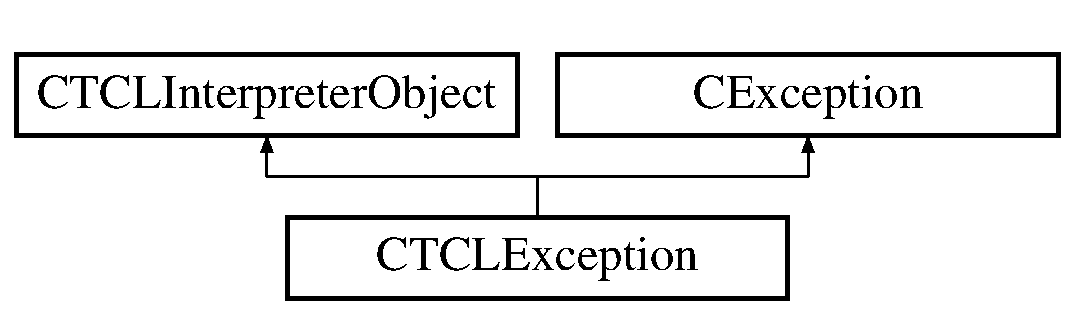
\includegraphics[height=2cm]{classCTCLException}
\end{center}
\end{figure}
\subsection*{Public Methods}
\begin{CompactItemize}
\item 
{\bf CTCLException} ({\bf CTCLInterpreter} \&am\_\-r\-Interpreter, {\bf Int\_\-t} am\_\-n\-Reason, const char $\ast$p\-String)
\item 
{\bf CTCLException} ({\bf CTCLInterpreter} \&am\_\-r\-Interpreter, {\bf Int\_\-t} am\_\-n\-Reason, const std::string \&r\-String)
\item 
virtual {\bf $\sim$CTCLException} ()
\item 
{\bf CTCLException} (const CTCLException \&a\-CTCLException)
\item 
CTCLException {\bf operator=} (const CTCLException \&a\-CTCLException)
\item 
int {\bf operator==} (const CTCLException \&a\-CTCLException)
\item 
{\bf Int\_\-t} {\bf get\-Reason} () const
\item 
void {\bf Add\-Error\-Info} (const char $\ast$p\-Message)
\item 
void {\bf Add\-Error\-Info} (const string \&r\-Message)
\item 
void {\bf Add\-Error\-Info} (const {\bf CTCLString} \&r\-Message)
\item 
void {\bf Set\-Error\-Code} (const char $\ast$p\-Message, const char $\ast$p\-Mnemonic=\char`\"{}???\char`\"{}, const char $\ast$p\-Facility=\char`\"{}TCL\char`\"{}, const char $\ast$p\-Severity=\char`\"{}FATAL\char`\"{})
\item 
void {\bf Set\-Error\-Code} (const string r\-Message, const string \&r\-Mnemonic=string(\char`\"{}???\char`\"{}), const string \&r\-Facility=string(\char`\"{}TCL\char`\"{}), const string \&r\-Severity=string(\char`\"{}FATAL\char`\"{}))
\item 
{\bf CTCLResult} {\bf Get\-Result} () const
\item 
virtual const char $\ast$ {\bf Reason\-Text} () const
\item 
virtual {\bf Int\_\-t} {\bf Reason\-Code} () const
\end{CompactItemize}
\subsection*{Protected Methods}
\begin{CompactItemize}
\item 
void {\bf set\-Interpreter} ({\bf CTCLInterpreter} \&am\_\-r\-Interpreter)
\item 
void {\bf set\-Reason} ({\bf Int\_\-t} am\_\-n\-Reason)
\end{CompactItemize}
\subsection*{Private Attributes}
\begin{CompactItemize}
\item 
{\bf Int\_\-t} {\bf m\_\-n\-Reason}
\end{CompactItemize}


\subsection{Constructor \& Destructor Documentation}
\index{CTCLException@{CTCLException}!CTCLException@{CTCLException}}
\index{CTCLException@{CTCLException}!CTCLException@{CTCLException}}
\subsubsection{\setlength{\rightskip}{0pt plus 5cm}CTCLException::CTCLException ({\bf CTCLInterpreter} \& {\em am\_\-r\-Interpreter}, {\bf Int\_\-t} {\em am\_\-n\-Reason}, const char $\ast$ {\em p\-String})\hspace{0.3cm}{\tt  [inline]}}\label{classCTCLException_a0}




Definition at line 331 of file TCLException.h.

References Int\_\-t, and m\_\-n\-Reason.\index{CTCLException@{CTCLException}!CTCLException@{CTCLException}}
\index{CTCLException@{CTCLException}!CTCLException@{CTCLException}}
\subsubsection{\setlength{\rightskip}{0pt plus 5cm}CTCLException::CTCLException ({\bf CTCLInterpreter} \& {\em am\_\-r\-Interpreter}, {\bf Int\_\-t} {\em am\_\-n\-Reason}, const std::string \& {\em r\-String})\hspace{0.3cm}{\tt  [inline]}}\label{classCTCLException_a1}




Definition at line 339 of file TCLException.h.

References Int\_\-t, and m\_\-n\-Reason.\index{CTCLException@{CTCLException}!~CTCLException@{$\sim$CTCLException}}
\index{~CTCLException@{$\sim$CTCLException}!CTCLException@{CTCLException}}
\subsubsection{\setlength{\rightskip}{0pt plus 5cm}virtual CTCLException::$\sim$CTCLException ()\hspace{0.3cm}{\tt  [inline, virtual]}}\label{classCTCLException_a2}




Definition at line 347 of file TCLException.h.\index{CTCLException@{CTCLException}!CTCLException@{CTCLException}}
\index{CTCLException@{CTCLException}!CTCLException@{CTCLException}}
\subsubsection{\setlength{\rightskip}{0pt plus 5cm}CTCLException::CTCLException (const CTCLException \& {\em a\-CTCLException})\hspace{0.3cm}{\tt  [inline]}}\label{classCTCLException_a3}




Definition at line 351 of file TCLException.h.

References m\_\-n\-Reason.

\subsection{Member Function Documentation}
\index{CTCLException@{CTCLException}!AddErrorInfo@{AddErrorInfo}}
\index{AddErrorInfo@{AddErrorInfo}!CTCLException@{CTCLException}}
\subsubsection{\setlength{\rightskip}{0pt plus 5cm}void CTCLException::Add\-Error\-Info (const {\bf CTCLString} \& {\em r\-Message})\hspace{0.3cm}{\tt  [inline]}}\label{classCTCLException_a9}




Definition at line 410 of file TCLException.h.

References Add\-Error\-Info().\index{CTCLException@{CTCLException}!AddErrorInfo@{AddErrorInfo}}
\index{AddErrorInfo@{AddErrorInfo}!CTCLException@{CTCLException}}
\subsubsection{\setlength{\rightskip}{0pt plus 5cm}void CTCLException::Add\-Error\-Info (const string \& {\em r\-Message})\hspace{0.3cm}{\tt  [inline]}}\label{classCTCLException_a8}




Definition at line 407 of file TCLException.h.

References Add\-Error\-Info().\index{CTCLException@{CTCLException}!AddErrorInfo@{AddErrorInfo}}
\index{AddErrorInfo@{AddErrorInfo}!CTCLException@{CTCLException}}
\subsubsection{\setlength{\rightskip}{0pt plus 5cm}void CTCLException::Add\-Error\-Info (const char $\ast$ {\em p\-Message})}\label{classCTCLException_a7}




Definition at line 313 of file TCLException.cpp.

References CTCLInterpreter::get\-Interpreter(), and CTCLInterpreter\-Object::get\-Interpreter().

Referenced by Add\-Error\-Info().\index{CTCLException@{CTCLException}!getReason@{getReason}}
\index{getReason@{getReason}!CTCLException@{CTCLException}}
\subsubsection{\setlength{\rightskip}{0pt plus 5cm}{\bf Int\_\-t} CTCLException::get\-Reason () const\hspace{0.3cm}{\tt  [inline]}}\label{classCTCLException_a6}




Definition at line 385 of file TCLException.h.

References Int\_\-t, and m\_\-n\-Reason.

Referenced by Reason\-Code().\index{CTCLException@{CTCLException}!GetResult@{GetResult}}
\index{GetResult@{GetResult}!CTCLException@{CTCLException}}
\subsubsection{\setlength{\rightskip}{0pt plus 5cm}{\bf CTCLResult} CTCLException::Get\-Result () const}\label{classCTCLException_a12}




Definition at line 407 of file TCLException.cpp.

References CTCLInterpreter\-Object::get\-Interpreter().

Referenced by Reason\-Text().\index{CTCLException@{CTCLException}!operator=@{operator=}}
\index{operator=@{operator=}!CTCLException@{CTCLException}}
\subsubsection{\setlength{\rightskip}{0pt plus 5cm}CTCLException CTCLException::operator= (const CTCLException \& {\em a\-CTCLException})\hspace{0.3cm}{\tt  [inline]}}\label{classCTCLException_a4}




Definition at line 360 of file TCLException.h.

References m\_\-n\-Reason, CException::operator=(), and CTCLInterpreter\-Object::operator=().\index{CTCLException@{CTCLException}!operator==@{operator==}}
\index{operator==@{operator==}!CTCLException@{CTCLException}}
\subsubsection{\setlength{\rightskip}{0pt plus 5cm}int CTCLException::operator== (const CTCLException \& {\em a\-CTCLException})\hspace{0.3cm}{\tt  [inline]}}\label{classCTCLException_a5}




Definition at line 373 of file TCLException.h.

References m\_\-n\-Reason, CException::operator==(), and CTCLInterpreter\-Object::operator==().\index{CTCLException@{CTCLException}!ReasonCode@{ReasonCode}}
\index{ReasonCode@{ReasonCode}!CTCLException@{CTCLException}}
\subsubsection{\setlength{\rightskip}{0pt plus 5cm}{\bf Int\_\-t} CTCLException::Reason\-Code () const\hspace{0.3cm}{\tt  [virtual]}}\label{classCTCLException_a14}


Returns a code which describes the reason for the exception . This is exception type specific and may be used to do detailed exception analysis and recovery. For example in the {\bf CErrno\-Exception} {\rm (p.\,\pageref{classCErrnoException})} class, the errno at the time of instantiation of the object is returned. The default returns -1 

Reimplemented from {\bf CException} {\rm (p.\,\pageref{classCException_a9})}.

Definition at line 390 of file TCLException.cpp.

References get\-Reason().\index{CTCLException@{CTCLException}!ReasonText@{ReasonText}}
\index{ReasonText@{ReasonText}!CTCLException@{CTCLException}}
\subsubsection{\setlength{\rightskip}{0pt plus 5cm}const char $\ast$ CTCLException::Reason\-Text () const\hspace{0.3cm}{\tt  [virtual]}}\label{classCTCLException_a13}


Returns a const pointer to text which describes the reason the exception was thrown. This is exception type specific. The default action returns a pointer to the constant string: \char`\"{}Unspecified Exception\char`\"{} 

Reimplemented from {\bf CException} {\rm (p.\,\pageref{classCException_a8})}.

Definition at line 374 of file TCLException.cpp.

References Get\-Result().\index{CTCLException@{CTCLException}!SetErrorCode@{SetErrorCode}}
\index{SetErrorCode@{SetErrorCode}!CTCLException@{CTCLException}}
\subsubsection{\setlength{\rightskip}{0pt plus 5cm}void CTCLException::Set\-Error\-Code (const string {\em r\-Message}, const string \& {\em r\-Mnemonic} = string(\char`\"{}???\char`\"{}), const string \& {\em r\-Facility} = string(\char`\"{}TCL\char`\"{}), const string \& {\em r\-Severity} = string(\char`\"{}FATAL\char`\"{}))\hspace{0.3cm}{\tt  [inline]}}\label{classCTCLException_a11}




Definition at line 418 of file TCLException.h.

References Set\-Error\-Code().\index{CTCLException@{CTCLException}!SetErrorCode@{SetErrorCode}}
\index{SetErrorCode@{SetErrorCode}!CTCLException@{CTCLException}}
\subsubsection{\setlength{\rightskip}{0pt plus 5cm}void CTCLException::Set\-Error\-Code (const char $\ast$ {\em p\-Message}, const char $\ast$ {\em p\-Mnemonic} = \char`\"{}???\char`\"{}, const char $\ast$ {\em p\-Facility} = \char`\"{}TCL\char`\"{}, const char $\ast$ {\em p\-Severity} = \char`\"{}FATAL\char`\"{})}\label{classCTCLException_a10}




Definition at line 339 of file TCLException.cpp.

References CTCLInterpreter::get\-Interpreter(), and CTCLInterpreter\-Object::get\-Interpreter().

Referenced by Set\-Error\-Code().\index{CTCLException@{CTCLException}!setInterpreter@{setInterpreter}}
\index{setInterpreter@{setInterpreter}!CTCLException@{CTCLException}}
\subsubsection{\setlength{\rightskip}{0pt plus 5cm}void CTCLException::set\-Interpreter ({\bf CTCLInterpreter} \& {\em am\_\-r\-Interpreter})\hspace{0.3cm}{\tt  [inline, protected]}}\label{classCTCLException_b0}




Definition at line 395 of file TCLException.h.

References CTCLInterpreter\-Object::Bind().\index{CTCLException@{CTCLException}!setReason@{setReason}}
\index{setReason@{setReason}!CTCLException@{CTCLException}}
\subsubsection{\setlength{\rightskip}{0pt plus 5cm}void CTCLException::set\-Reason ({\bf Int\_\-t} {\em am\_\-n\-Reason})\hspace{0.3cm}{\tt  [inline, protected]}}\label{classCTCLException_b1}




Definition at line 399 of file TCLException.h.

References Int\_\-t, and m\_\-n\-Reason.

\subsection{Member Data Documentation}
\index{CTCLException@{CTCLException}!m_nReason@{m\_\-nReason}}
\index{m_nReason@{m\_\-nReason}!CTCLException@{CTCLException}}
\subsubsection{\setlength{\rightskip}{0pt plus 5cm}{\bf Int\_\-t} CTCLException::m\_\-n\-Reason\hspace{0.3cm}{\tt  [private]}}\label{classCTCLException_o0}




Definition at line 321 of file TCLException.h.

Referenced by CTCLException(), get\-Reason(), operator=(), operator==(), and set\-Reason().

The documentation for this class was generated from the following files:\begin{CompactItemize}
\item 
{\bf TCLException.h}\item 
{\bf TCLException.cpp}\end{CompactItemize}

\section{CTCLFile\-Handler  Class Reference}
\label{classCTCLFileHandler}\index{CTCLFileHandler@{CTCLFile\-Handler}}
{\tt \#include $<$TCLFile\-Handler.h$>$}

Inheritance diagram for CTCLFile\-Handler::\begin{figure}[H]
\begin{center}
\leavevmode
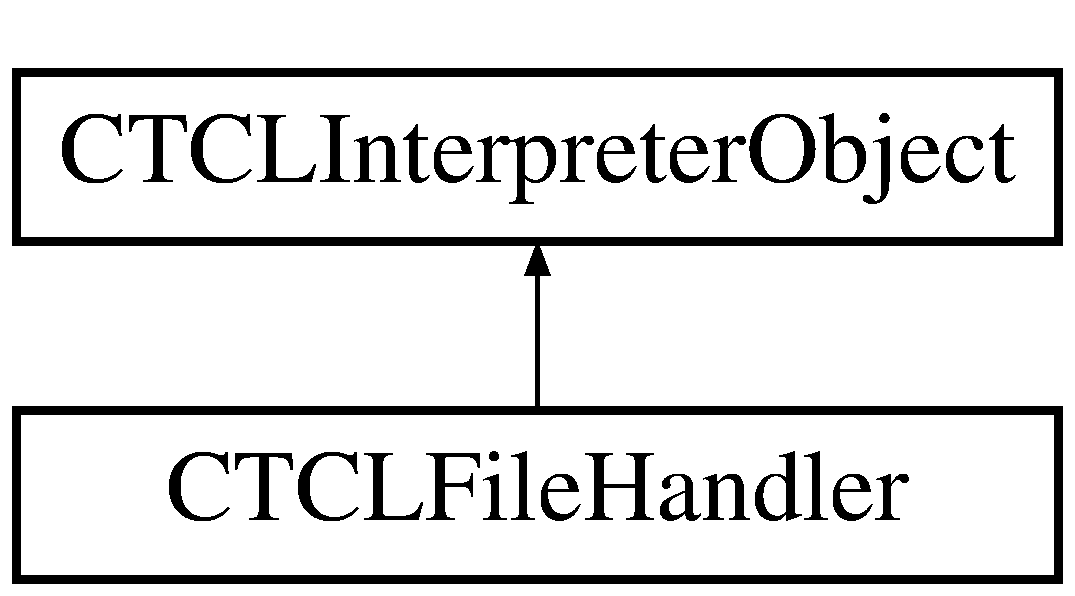
\includegraphics[height=2cm]{classCTCLFileHandler}
\end{center}
\end{figure}
\subsection*{Public Methods}
\begin{CompactItemize}
\item 
{\bf CTCLFile\-Handler} ({\bf CTCLInterpreter\-Object} $\ast$p\-Interp, {\bf UInt\_\-t} am\_\-n\-Fid=STDIN\_\-FILENO)
\item 
{\bf CTCLFile\-Handler} ({\bf CTCLInterpreter\-Object} $\ast$p\-Interp, FILE $\ast$p\-File)
\item 
{\bf CTCLFile\-Handler} ({\bf CTCLInterpreter\-Object} $\ast$p\-Interp, fstream \&r\-File)
\item 
{\bf CTCLFile\-Handler} ({\bf CTCLInterpreter} $\ast$p\-Interp, {\bf UInt\_\-t} am\_\-n\-Fid=STDIN\_\-FILENO)
\item 
{\bf CTCLFile\-Handler} ({\bf CTCLInterpreter} $\ast$p\-Interp, FILE $\ast$p\-File)
\item 
{\bf CTCLFile\-Handler} ({\bf CTCLInterpreter} $\ast$p\-Interp, fstream \&r\-File)
\item 
{\bf $\sim$CTCLFile\-Handler} ()
\item 
{\bf CTCLFile\-Handler} (const CTCLFile\-Handler \&a\-CTCLFile\-Handler)
\item 
CTCLFile\-Handler \& {\bf operator=} (const CTCLFile\-Handler \&a\-CTCLFile\-Handler)
\item 
int {\bf operator==} (const CTCLFile\-Handler \&a\-CTCLFile\-Handler) const
\item 
{\bf UInt\_\-t} {\bf get\-Fid} () const
\item 
void {\bf set\-Fid} ({\bf UInt\_\-t} am\_\-n\-Fid)
\item 
virtual void {\bf operator()} (int mask)=0
\item 
void {\bf Set} (int mask)
\item 
void {\bf Clear} ()
\end{CompactItemize}
\subsection*{Static Public Methods}
\begin{CompactItemize}
\item 
void {\bf Callback\-Relay} (Client\-Data p\-Object, int mask)
\end{CompactItemize}
\subsection*{Private Attributes}
\begin{CompactItemize}
\item 
{\bf UInt\_\-t} {\bf m\_\-n\-Fid}
\end{CompactItemize}


\subsection{Constructor \& Destructor Documentation}
\index{CTCLFileHandler@{CTCLFile\-Handler}!CTCLFileHandler@{CTCLFileHandler}}
\index{CTCLFileHandler@{CTCLFileHandler}!CTCLFileHandler@{CTCLFile\-Handler}}
\subsubsection{\setlength{\rightskip}{0pt plus 5cm}CTCLFile\-Handler::CTCLFile\-Handler ({\bf CTCLInterpreter\-Object} $\ast$ {\em p\-Interp}, {\bf UInt\_\-t} {\em am\_\-n\-Fid} = STDIN\_\-FILENO)\hspace{0.3cm}{\tt  [inline]}}\label{classCTCLFileHandler_a0}




Definition at line 327 of file TCLFile\-Handler.h.

References CTCLInterpreter\-Object::get\-Interpreter(), m\_\-n\-Fid, and UInt\_\-t.\index{CTCLFileHandler@{CTCLFile\-Handler}!CTCLFileHandler@{CTCLFileHandler}}
\index{CTCLFileHandler@{CTCLFileHandler}!CTCLFileHandler@{CTCLFile\-Handler}}
\subsubsection{\setlength{\rightskip}{0pt plus 5cm}CTCLFile\-Handler::CTCLFile\-Handler ({\bf CTCLInterpreter\-Object} $\ast$ {\em p\-Interp}, FILE $\ast$ {\em p\-File})\hspace{0.3cm}{\tt  [inline]}}\label{classCTCLFileHandler_a1}




Definition at line 332 of file TCLFile\-Handler.h.

References CTCLInterpreter\-Object::get\-Interpreter(), and m\_\-n\-Fid.\index{CTCLFileHandler@{CTCLFile\-Handler}!CTCLFileHandler@{CTCLFileHandler}}
\index{CTCLFileHandler@{CTCLFileHandler}!CTCLFileHandler@{CTCLFile\-Handler}}
\subsubsection{\setlength{\rightskip}{0pt plus 5cm}CTCLFile\-Handler::CTCLFile\-Handler ({\bf CTCLInterpreter\-Object} $\ast$ {\em p\-Interp}, fstream \& {\em r\-File})\hspace{0.3cm}{\tt  [inline]}}\label{classCTCLFileHandler_a2}




Definition at line 337 of file TCLFile\-Handler.h.

References m\_\-n\-Fid.\index{CTCLFileHandler@{CTCLFile\-Handler}!CTCLFileHandler@{CTCLFileHandler}}
\index{CTCLFileHandler@{CTCLFileHandler}!CTCLFileHandler@{CTCLFile\-Handler}}
\subsubsection{\setlength{\rightskip}{0pt plus 5cm}CTCLFile\-Handler::CTCLFile\-Handler ({\bf CTCLInterpreter} $\ast$ {\em p\-Interp}, {\bf UInt\_\-t} {\em am\_\-n\-Fid} = STDIN\_\-FILENO)\hspace{0.3cm}{\tt  [inline]}}\label{classCTCLFileHandler_a3}




Definition at line 342 of file TCLFile\-Handler.h.

References m\_\-n\-Fid, and UInt\_\-t.\index{CTCLFileHandler@{CTCLFile\-Handler}!CTCLFileHandler@{CTCLFileHandler}}
\index{CTCLFileHandler@{CTCLFileHandler}!CTCLFileHandler@{CTCLFile\-Handler}}
\subsubsection{\setlength{\rightskip}{0pt plus 5cm}CTCLFile\-Handler::CTCLFile\-Handler ({\bf CTCLInterpreter} $\ast$ {\em p\-Interp}, FILE $\ast$ {\em p\-File})\hspace{0.3cm}{\tt  [inline]}}\label{classCTCLFileHandler_a4}




Definition at line 347 of file TCLFile\-Handler.h.

References m\_\-n\-Fid.\index{CTCLFileHandler@{CTCLFile\-Handler}!CTCLFileHandler@{CTCLFileHandler}}
\index{CTCLFileHandler@{CTCLFileHandler}!CTCLFileHandler@{CTCLFile\-Handler}}
\subsubsection{\setlength{\rightskip}{0pt plus 5cm}CTCLFile\-Handler::CTCLFile\-Handler ({\bf CTCLInterpreter} $\ast$ {\em p\-Interp}, fstream \& {\em r\-File})\hspace{0.3cm}{\tt  [inline]}}\label{classCTCLFileHandler_a5}




Definition at line 352 of file TCLFile\-Handler.h.

References m\_\-n\-Fid.\index{CTCLFileHandler@{CTCLFile\-Handler}!~CTCLFileHandler@{$\sim$CTCLFileHandler}}
\index{~CTCLFileHandler@{$\sim$CTCLFileHandler}!CTCLFileHandler@{CTCLFile\-Handler}}
\subsubsection{\setlength{\rightskip}{0pt plus 5cm}CTCLFile\-Handler::$\sim$CTCLFile\-Handler ()\hspace{0.3cm}{\tt  [inline]}}\label{classCTCLFileHandler_a6}




Definition at line 357 of file TCLFile\-Handler.h.

References Clear().\index{CTCLFileHandler@{CTCLFile\-Handler}!CTCLFileHandler@{CTCLFileHandler}}
\index{CTCLFileHandler@{CTCLFileHandler}!CTCLFileHandler@{CTCLFile\-Handler}}
\subsubsection{\setlength{\rightskip}{0pt plus 5cm}CTCLFile\-Handler::CTCLFile\-Handler (const CTCLFile\-Handler \& {\em a\-CTCLFile\-Handler})\hspace{0.3cm}{\tt  [inline]}}\label{classCTCLFileHandler_a7}




Definition at line 360 of file TCLFile\-Handler.h.

References m\_\-n\-Fid.

\subsection{Member Function Documentation}
\index{CTCLFileHandler@{CTCLFile\-Handler}!CallbackRelay@{CallbackRelay}}
\index{CallbackRelay@{CallbackRelay}!CTCLFileHandler@{CTCLFile\-Handler}}
\subsubsection{\setlength{\rightskip}{0pt plus 5cm}void CTCLFile\-Handler::Callback\-Relay (Client\-Data {\em p\-Object}, int {\em mask})\hspace{0.3cm}{\tt  [static]}}\label{classCTCLFileHandler_d0}




Definition at line 321 of file TCLFile\-Handler.cpp.

Referenced by Set().\index{CTCLFileHandler@{CTCLFile\-Handler}!Clear@{Clear}}
\index{Clear@{Clear}!CTCLFileHandler@{CTCLFile\-Handler}}
\subsubsection{\setlength{\rightskip}{0pt plus 5cm}void CTCLFile\-Handler::Clear ()}\label{classCTCLFileHandler_a14}




Definition at line 372 of file TCLFile\-Handler.cpp.

References m\_\-n\-Fid.

Referenced by $\sim$CTCLFile\-Handler().\index{CTCLFileHandler@{CTCLFile\-Handler}!getFid@{getFid}}
\index{getFid@{getFid}!CTCLFileHandler@{CTCLFile\-Handler}}
\subsubsection{\setlength{\rightskip}{0pt plus 5cm}{\bf UInt\_\-t} CTCLFile\-Handler::get\-Fid () const\hspace{0.3cm}{\tt  [inline]}}\label{classCTCLFileHandler_a10}




Definition at line 388 of file TCLFile\-Handler.h.

References m\_\-n\-Fid, and UInt\_\-t.\index{CTCLFileHandler@{CTCLFile\-Handler}!operator()@{operator()}}
\index{operator()@{operator()}!CTCLFileHandler@{CTCLFile\-Handler}}
\subsubsection{\setlength{\rightskip}{0pt plus 5cm}virtual void CTCLFile\-Handler::operator() (int {\em mask})\hspace{0.3cm}{\tt  [pure virtual]}}\label{classCTCLFileHandler_a12}


\index{CTCLFileHandler@{CTCLFile\-Handler}!operator=@{operator=}}
\index{operator=@{operator=}!CTCLFileHandler@{CTCLFile\-Handler}}
\subsubsection{\setlength{\rightskip}{0pt plus 5cm}CTCLFile\-Handler\& CTCLFile\-Handler::operator= (const CTCLFile\-Handler \& {\em a\-CTCLFile\-Handler})\hspace{0.3cm}{\tt  [inline]}}\label{classCTCLFileHandler_a8}




Definition at line 369 of file TCLFile\-Handler.h.

References m\_\-n\-Fid, and CTCLInterpreter\-Object::operator=().\index{CTCLFileHandler@{CTCLFile\-Handler}!operator==@{operator==}}
\index{operator==@{operator==}!CTCLFileHandler@{CTCLFile\-Handler}}
\subsubsection{\setlength{\rightskip}{0pt plus 5cm}int CTCLFile\-Handler::operator== (const CTCLFile\-Handler \& {\em a\-CTCLFile\-Handler}) const\hspace{0.3cm}{\tt  [inline]}}\label{classCTCLFileHandler_a9}




Definition at line 379 of file TCLFile\-Handler.h.

References m\_\-n\-Fid, and CTCLInterpreter\-Object::operator==().\index{CTCLFileHandler@{CTCLFile\-Handler}!Set@{Set}}
\index{Set@{Set}!CTCLFileHandler@{CTCLFile\-Handler}}
\subsubsection{\setlength{\rightskip}{0pt plus 5cm}void CTCLFile\-Handler::Set (int {\em mask})}\label{classCTCLFileHandler_a13}




Definition at line 348 of file TCLFile\-Handler.cpp.

References Callback\-Relay(), and m\_\-n\-Fid.\index{CTCLFileHandler@{CTCLFile\-Handler}!setFid@{setFid}}
\index{setFid@{setFid}!CTCLFileHandler@{CTCLFile\-Handler}}
\subsubsection{\setlength{\rightskip}{0pt plus 5cm}void CTCLFile\-Handler::set\-Fid ({\bf UInt\_\-t} {\em am\_\-n\-Fid})\hspace{0.3cm}{\tt  [inline]}}\label{classCTCLFileHandler_a11}




Definition at line 395 of file TCLFile\-Handler.h.

References m\_\-n\-Fid, and UInt\_\-t.

\subsection{Member Data Documentation}
\index{CTCLFileHandler@{CTCLFile\-Handler}!m_nFid@{m\_\-nFid}}
\index{m_nFid@{m\_\-nFid}!CTCLFileHandler@{CTCLFile\-Handler}}
\subsubsection{\setlength{\rightskip}{0pt plus 5cm}{\bf UInt\_\-t} CTCLFile\-Handler::m\_\-n\-Fid\hspace{0.3cm}{\tt  [private]}}\label{classCTCLFileHandler_o0}




Definition at line 322 of file TCLFile\-Handler.h.

Referenced by Clear(), CTCLFile\-Handler(), get\-Fid(), operator=(), operator==(), Set(), and set\-Fid().

The documentation for this class was generated from the following files:\begin{CompactItemize}
\item 
{\bf TCLFile\-Handler.h}\item 
{\bf TCLFile\-Handler.cpp}\end{CompactItemize}

\section{CTCLHash\-Table$<$ T $>$  Class Template Reference}
\label{classCTCLHashTable}\index{CTCLHashTable@{CTCLHash\-Table}}
{\tt \#include $<$TCLHash\-Table.h$>$}

\subsection*{Public Methods}
\begin{CompactItemize}
\item 
{\bf CTCLHash\-Table} ()
\item 
virtual {\bf $\sim$CTCLHash\-Table} ()
\item 
{\bf CTCLHash\-Table} (Tcl\_\-Hash\-Table am\_\-Hash\-Table)
\item 
{\bf CTCLHash\-Table} (const CTCLHash\-Table \&a\-CTCLHash\-Table)
\item 
CTCLHash\-Table {\bf operator=} (const CTCLHash\-Table \&a\-CTCLHash\-Table)
\item 
int {\bf operator==} (const CTCLHash\-Table \&a\-CTCLHash\-Table)
\item 
Tcl\_\-Hash\-Table $\ast$ {\bf get\-Hash\-Table} () const
\item 
void {\bf Enter} (const std::string \&r\-Key, {\bf r\-CTCLTHash\-Table\-Item} r\-Value)
\item 
const {\bf CTCLTHash\-Table\-Item} $\ast$ {\bf Find} (const std::string \&rs\-Keyword) const
\item 
{\bf CTCLTHash\-Table\-Item} $\ast$ {\bf Delete} (const std::string \&rs\-Keyword)
\item 
{\bf CTCLTHash\-Table\-Iterator} {\bf begin} ()
\item 
{\bf CTCLTHash\-Table\-Iterator} {\bf end} ()
\item 
std::string {\bf Statistics} ()
\end{CompactItemize}
\subsection*{Protected Methods}
\begin{CompactItemize}
\item 
void {\bf set\-Hash\-Table} (Tcl\_\-Hash\-Table $\ast$am\_\-Hash\-Table)
\end{CompactItemize}
\subsection*{Private Types}
\begin{CompactItemize}
\item 
typedef {\bf CTCLHash\-Table\-Item}$<$ T $>$ {\bf CTCLTHash\-Table\-Item}
\item 
typedef {\bf CTCLHash\-Table\-Item}$<$ T $>$ $\ast$ {\bf p\-CTCLTHash\-Table\-Item}
\item 
typedef {\bf CTCLHash\-Table\-Item}$<$ T $>$ \& {\bf r\-CTCLTHash\-Table\-Item}
\item 
typedef {\bf CTCLHash\-Table\-Iterator}$<$ T $>$ {\bf CTCLTHash\-Table\-Iterator}
\item 
typedef {\bf CTCLHash\-Table\-Iterator}$<$ T $>$ $\ast$ {\bf p\-CTCLTHash\-Table\-Iterator}
\item 
typedef {\bf CTCLHash\-Table\-Iterator}$<$ T $>$ \& {\bf r\-CTCLTHash\-Table\-Iterator}
\end{CompactItemize}
\subsection*{Private Attributes}
\begin{CompactItemize}
\item 
Tcl\_\-Hash\-Table {\bf m\_\-Hash\-Table}
\end{CompactItemize}
\subsubsection*{template$<$class T$>$ class CTCLHash\-Table$<$ T $>$}



\subsection{Member Typedef Documentation}
\index{CTCLHashTable@{CTCLHash\-Table}!CTCLTHashTableItem@{CTCLTHashTableItem}}
\index{CTCLTHashTableItem@{CTCLTHashTableItem}!CTCLHashTable@{CTCLHash\-Table}}
\subsubsection{\setlength{\rightskip}{0pt plus 5cm}template$<$class T$>$ typedef {\bf CTCLHash\-Table\-Item}$<$T$>$ CTCLHash\-Table$<$ T $>$::CTCLTHash\-Table\-Item\hspace{0.3cm}{\tt  [private]}}\label{classCTCLHashTable_u0}




Definition at line 327 of file TCLHash\-Table.h.\index{CTCLHashTable@{CTCLHash\-Table}!CTCLTHashTableIterator@{CTCLTHashTableIterator}}
\index{CTCLTHashTableIterator@{CTCLTHashTableIterator}!CTCLHashTable@{CTCLHash\-Table}}
\subsubsection{\setlength{\rightskip}{0pt plus 5cm}template$<$class T$>$ typedef {\bf CTCLHash\-Table\-Iterator}$<$T$>$ CTCLHash\-Table$<$ T $>$::CTCLTHash\-Table\-Iterator\hspace{0.3cm}{\tt  [private]}}\label{classCTCLHashTable_u3}




Definition at line 331 of file TCLHash\-Table.h.\index{CTCLHashTable@{CTCLHash\-Table}!pCTCLTHashTableItem@{pCTCLTHashTableItem}}
\index{pCTCLTHashTableItem@{pCTCLTHashTableItem}!CTCLHashTable@{CTCLHash\-Table}}
\subsubsection{\setlength{\rightskip}{0pt plus 5cm}template$<$class T$>$ typedef {\bf CTCLHash\-Table\-Item}$<$T$>$ $\ast$ CTCLHash\-Table$<$ T $>$::p\-CTCLTHash\-Table\-Item\hspace{0.3cm}{\tt  [private]}}\label{classCTCLHashTable_u1}




Definition at line 327 of file TCLHash\-Table.h.\index{CTCLHashTable@{CTCLHash\-Table}!pCTCLTHashTableIterator@{pCTCLTHashTableIterator}}
\index{pCTCLTHashTableIterator@{pCTCLTHashTableIterator}!CTCLHashTable@{CTCLHash\-Table}}
\subsubsection{\setlength{\rightskip}{0pt plus 5cm}template$<$class T$>$ typedef {\bf CTCLHash\-Table\-Iterator}$<$T$>$ $\ast$ CTCLHash\-Table$<$ T $>$::p\-CTCLTHash\-Table\-Iterator\hspace{0.3cm}{\tt  [private]}}\label{classCTCLHashTable_u4}




Definition at line 331 of file TCLHash\-Table.h.\index{CTCLHashTable@{CTCLHash\-Table}!rCTCLTHashTableItem@{rCTCLTHashTableItem}}
\index{rCTCLTHashTableItem@{rCTCLTHashTableItem}!CTCLHashTable@{CTCLHash\-Table}}
\subsubsection{\setlength{\rightskip}{0pt plus 5cm}template$<$class T$>$ typedef {\bf CTCLHash\-Table\-Item}$<$T$>$ \& CTCLHash\-Table$<$ T $>$::r\-CTCLTHash\-Table\-Item\hspace{0.3cm}{\tt  [private]}}\label{classCTCLHashTable_u2}




Definition at line 327 of file TCLHash\-Table.h.\index{CTCLHashTable@{CTCLHash\-Table}!rCTCLTHashTableIterator@{rCTCLTHashTableIterator}}
\index{rCTCLTHashTableIterator@{rCTCLTHashTableIterator}!CTCLHashTable@{CTCLHash\-Table}}
\subsubsection{\setlength{\rightskip}{0pt plus 5cm}template$<$class T$>$ typedef {\bf CTCLHash\-Table\-Iterator}$<$T$>$ \& CTCLHash\-Table$<$ T $>$::r\-CTCLTHash\-Table\-Iterator\hspace{0.3cm}{\tt  [private]}}\label{classCTCLHashTable_u5}




Definition at line 331 of file TCLHash\-Table.h.

\subsection{Constructor \& Destructor Documentation}
\index{CTCLHashTable@{CTCLHash\-Table}!CTCLHashTable@{CTCLHashTable}}
\index{CTCLHashTable@{CTCLHashTable}!CTCLHashTable@{CTCLHash\-Table}}
\subsubsection{\setlength{\rightskip}{0pt plus 5cm}template$<$class T$>$ CTCLHash\-Table$<$ T $>$::CTCLHash\-Table ()\hspace{0.3cm}{\tt  [inline]}}\label{classCTCLHashTable_a0}




Definition at line 340 of file TCLHash\-Table.h.

References CTCLHash\-Table$<$ T $>$::m\_\-Hash\-Table.\index{CTCLHashTable@{CTCLHash\-Table}!~CTCLHashTable@{$\sim$CTCLHashTable}}
\index{~CTCLHashTable@{$\sim$CTCLHashTable}!CTCLHashTable@{CTCLHash\-Table}}
\subsubsection{\setlength{\rightskip}{0pt plus 5cm}template$<$class T$>$ virtual CTCLHash\-Table$<$ T $>$::$\sim$CTCLHash\-Table ()\hspace{0.3cm}{\tt  [inline, virtual]}}\label{classCTCLHashTable_a1}




Definition at line 344 of file TCLHash\-Table.h.\index{CTCLHashTable@{CTCLHash\-Table}!CTCLHashTable@{CTCLHashTable}}
\index{CTCLHashTable@{CTCLHashTable}!CTCLHashTable@{CTCLHash\-Table}}
\subsubsection{\setlength{\rightskip}{0pt plus 5cm}template$<$class T$>$ CTCLHash\-Table$<$ T $>$::CTCLHash\-Table (Tcl\_\-Hash\-Table {\em am\_\-Hash\-Table})\hspace{0.3cm}{\tt  [inline]}}\label{classCTCLHashTable_a2}




Definition at line 349 of file TCLHash\-Table.h.

References CTCLHash\-Table$<$ T $>$::m\_\-Hash\-Table.\index{CTCLHashTable@{CTCLHash\-Table}!CTCLHashTable@{CTCLHashTable}}
\index{CTCLHashTable@{CTCLHashTable}!CTCLHashTable@{CTCLHash\-Table}}
\subsubsection{\setlength{\rightskip}{0pt plus 5cm}template$<$class T$>$ CTCLHash\-Table$<$ T $>$::CTCLHash\-Table (const CTCLHash\-Table$<$ T $>$ \& {\em a\-CTCLHash\-Table})\hspace{0.3cm}{\tt  [inline]}}\label{classCTCLHashTable_a3}




Definition at line 355 of file TCLHash\-Table.h.

References CTCLHash\-Table$<$ T $>$::m\_\-Hash\-Table.

\subsection{Member Function Documentation}
\index{CTCLHashTable@{CTCLHash\-Table}!begin@{begin}}
\index{begin@{begin}!CTCLHashTable@{CTCLHash\-Table}}
\subsubsection{\setlength{\rightskip}{0pt plus 5cm}template$<$class T$>$ {\bf CTCLTHash\-Table\-Iterator} CTCLHash\-Table$<$ T $>$::begin ()\hspace{0.3cm}{\tt  [inline]}}\label{classCTCLHashTable_a10}




Definition at line 426 of file TCLHash\-Table.h.\index{CTCLHashTable@{CTCLHash\-Table}!Delete@{Delete}}
\index{Delete@{Delete}!CTCLHashTable@{CTCLHash\-Table}}
\subsubsection{\setlength{\rightskip}{0pt plus 5cm}template$<$class T$>$ {\bf CTCLTHash\-Table\-Item}$\ast$ CTCLHash\-Table$<$ T $>$::Delete (const std::string \& {\em rs\-Keyword})\hspace{0.3cm}{\tt  [inline]}}\label{classCTCLHashTable_a9}




Definition at line 413 of file TCLHash\-Table.h.\index{CTCLHashTable@{CTCLHash\-Table}!end@{end}}
\index{end@{end}!CTCLHashTable@{CTCLHash\-Table}}
\subsubsection{\setlength{\rightskip}{0pt plus 5cm}template$<$class T$>$ {\bf CTCLTHash\-Table\-Iterator} CTCLHash\-Table$<$ T $>$::end ()\hspace{0.3cm}{\tt  [inline]}}\label{classCTCLHashTable_a11}




Definition at line 431 of file TCLHash\-Table.h.\index{CTCLHashTable@{CTCLHash\-Table}!Enter@{Enter}}
\index{Enter@{Enter}!CTCLHashTable@{CTCLHash\-Table}}
\subsubsection{\setlength{\rightskip}{0pt plus 5cm}template$<$class T$>$ void CTCLHash\-Table$<$ T $>$::Enter (const std::string \& {\em r\-Key}, {\bf r\-CTCLTHash\-Table\-Item} {\em r\-Value})\hspace{0.3cm}{\tt  [inline]}}\label{classCTCLHashTable_a7}




Definition at line 396 of file TCLHash\-Table.h.

References Int\_\-t.\index{CTCLHashTable@{CTCLHash\-Table}!Find@{Find}}
\index{Find@{Find}!CTCLHashTable@{CTCLHash\-Table}}
\subsubsection{\setlength{\rightskip}{0pt plus 5cm}template$<$class T$>$ const {\bf CTCLTHash\-Table\-Item}$\ast$ CTCLHash\-Table$<$ T $>$::Find (const std::string \& {\em rs\-Keyword}) const\hspace{0.3cm}{\tt  [inline]}}\label{classCTCLHashTable_a8}




Definition at line 405 of file TCLHash\-Table.h.\index{CTCLHashTable@{CTCLHash\-Table}!getHashTable@{getHashTable}}
\index{getHashTable@{getHashTable}!CTCLHashTable@{CTCLHash\-Table}}
\subsubsection{\setlength{\rightskip}{0pt plus 5cm}template$<$class T$>$ Tcl\_\-Hash\-Table$\ast$ CTCLHash\-Table$<$ T $>$::get\-Hash\-Table () const\hspace{0.3cm}{\tt  [inline]}}\label{classCTCLHashTable_a6}




Definition at line 381 of file TCLHash\-Table.h.

References CTCLHash\-Table$<$ T $>$::m\_\-Hash\-Table.\index{CTCLHashTable@{CTCLHash\-Table}!operator=@{operator=}}
\index{operator=@{operator=}!CTCLHashTable@{CTCLHash\-Table}}
\subsubsection{\setlength{\rightskip}{0pt plus 5cm}template$<$class T$>$ CTCLHash\-Table CTCLHash\-Table$<$ T $>$::operator= (const CTCLHash\-Table$<$ T $>$ \& {\em a\-CTCLHash\-Table})\hspace{0.3cm}{\tt  [inline]}}\label{classCTCLHashTable_a4}




Definition at line 362 of file TCLHash\-Table.h.

References CTCLHash\-Table$<$ T $>$::m\_\-Hash\-Table.\index{CTCLHashTable@{CTCLHash\-Table}!operator==@{operator==}}
\index{operator==@{operator==}!CTCLHashTable@{CTCLHash\-Table}}
\subsubsection{\setlength{\rightskip}{0pt plus 5cm}template$<$class T$>$ int CTCLHash\-Table$<$ T $>$::operator== (const CTCLHash\-Table$<$ T $>$ \& {\em a\-CTCLHash\-Table})\hspace{0.3cm}{\tt  [inline]}}\label{classCTCLHashTable_a5}




Definition at line 372 of file TCLHash\-Table.h.

References CTCLHash\-Table$<$ T $>$::m\_\-Hash\-Table.\index{CTCLHashTable@{CTCLHash\-Table}!setHashTable@{setHashTable}}
\index{setHashTable@{setHashTable}!CTCLHashTable@{CTCLHash\-Table}}
\subsubsection{\setlength{\rightskip}{0pt plus 5cm}template$<$class T$>$ void CTCLHash\-Table$<$ T $>$::set\-Hash\-Table (Tcl\_\-Hash\-Table $\ast$ {\em am\_\-Hash\-Table})\hspace{0.3cm}{\tt  [inline, protected]}}\label{classCTCLHashTable_b0}




Definition at line 389 of file TCLHash\-Table.h.

References CTCLHash\-Table$<$ T $>$::m\_\-Hash\-Table.\index{CTCLHashTable@{CTCLHash\-Table}!Statistics@{Statistics}}
\index{Statistics@{Statistics}!CTCLHashTable@{CTCLHash\-Table}}
\subsubsection{\setlength{\rightskip}{0pt plus 5cm}template$<$class T$>$ std::string CTCLHash\-Table$<$ T $>$::Statistics ()\hspace{0.3cm}{\tt  [inline]}}\label{classCTCLHashTable_a12}




Definition at line 438 of file TCLHash\-Table.h.

\subsection{Member Data Documentation}
\index{CTCLHashTable@{CTCLHash\-Table}!m_HashTable@{m\_\-HashTable}}
\index{m_HashTable@{m\_\-HashTable}!CTCLHashTable@{CTCLHash\-Table}}
\subsubsection{\setlength{\rightskip}{0pt plus 5cm}template$<$class T$>$ Tcl\_\-Hash\-Table CTCLHash\-Table$<$ T $>$::m\_\-Hash\-Table\hspace{0.3cm}{\tt  [private]}}\label{classCTCLHashTable_o0}




Definition at line 335 of file TCLHash\-Table.h.

Referenced by CTCLHash\-Table$<$ T $>$::CTCLHash\-Table(), CTCLHash\-Table$<$ T $>$::get\-Hash\-Table(), CTCLHash\-Table$<$ T $>$::operator=(), CTCLHash\-Table$<$ T $>$::operator==(), and CTCLHash\-Table$<$ T $>$::set\-Hash\-Table().

The documentation for this class was generated from the following file:\begin{CompactItemize}
\item 
{\bf TCLHash\-Table.h}\end{CompactItemize}

\section{CTCLHash\-Table\-Item$<$ T $>$  Class Template Reference}
\label{classCTCLHashTableItem}\index{CTCLHashTableItem@{CTCLHash\-Table\-Item}}
{\tt \#include $<$TCLHash\-Table\-Item.h$>$}

\subsection*{Public Methods}
\begin{CompactItemize}
\item 
{\bf CTCLHash\-Table\-Item} (T am\_\-Item)
\item 
virtual {\bf $\sim$CTCLHash\-Table\-Item} ()
\item 
{\bf CTCLHash\-Table\-Item} (const CTCLHash\-Table\-Item \&a\-CTCLHash\-Table\-Item)
\item 
CTCLHash\-Table\-Item {\bf operator=} (const CTCLHash\-Table\-Item \&a\-CTCLHash\-Table\-Item)
\item 
int {\bf operator==} (const CTCLHash\-Table\-Item \&a\-CTCLHash\-Table\-Item)
\item 
T {\bf get\-Item} () const
\end{CompactItemize}
\subsection*{Protected Methods}
\begin{CompactItemize}
\item 
void {\bf setm\_\-Item} (T am\_\-Item)
\item 
T \& {\bf operator $\ast$} ()
\item 
T $\ast$ {\bf operator $\rightarrow$ } ()
\end{CompactItemize}
\subsection*{Private Attributes}
\begin{CompactItemize}
\item 
T {\bf m\_\-Item}
\end{CompactItemize}
\subsubsection*{template$<$class T$>$ class CTCLHash\-Table\-Item$<$ T $>$}



\subsection{Constructor \& Destructor Documentation}
\index{CTCLHashTableItem@{CTCLHash\-Table\-Item}!CTCLHashTableItem@{CTCLHashTableItem}}
\index{CTCLHashTableItem@{CTCLHashTableItem}!CTCLHashTableItem@{CTCLHash\-Table\-Item}}
\subsubsection{\setlength{\rightskip}{0pt plus 5cm}template$<$class T$>$ CTCLHash\-Table\-Item$<$ T $>$::CTCLHash\-Table\-Item (T {\em am\_\-Item})\hspace{0.3cm}{\tt  [inline]}}\label{classCTCLHashTableItem_a0}




Definition at line 307 of file TCLHash\-Table\-Item.h.

References CTCLHash\-Table\-Item$<$ T $>$::m\_\-Item.\index{CTCLHashTableItem@{CTCLHash\-Table\-Item}!~CTCLHashTableItem@{$\sim$CTCLHashTableItem}}
\index{~CTCLHashTableItem@{$\sim$CTCLHashTableItem}!CTCLHashTableItem@{CTCLHash\-Table\-Item}}
\subsubsection{\setlength{\rightskip}{0pt plus 5cm}template$<$class T$>$ virtual CTCLHash\-Table\-Item$<$ T $>$::$\sim$CTCLHash\-Table\-Item ()\hspace{0.3cm}{\tt  [inline, virtual]}}\label{classCTCLHashTableItem_a1}




Definition at line 309 of file TCLHash\-Table\-Item.h.\index{CTCLHashTableItem@{CTCLHash\-Table\-Item}!CTCLHashTableItem@{CTCLHashTableItem}}
\index{CTCLHashTableItem@{CTCLHashTableItem}!CTCLHashTableItem@{CTCLHash\-Table\-Item}}
\subsubsection{\setlength{\rightskip}{0pt plus 5cm}template$<$class T$>$ CTCLHash\-Table\-Item$<$ T $>$::CTCLHash\-Table\-Item (const CTCLHash\-Table\-Item$<$ T $>$ \& {\em a\-CTCLHash\-Table\-Item})\hspace{0.3cm}{\tt  [inline]}}\label{classCTCLHashTableItem_a2}




Definition at line 313 of file TCLHash\-Table\-Item.h.

References CTCLHash\-Table\-Item$<$ T $>$::m\_\-Item.

\subsection{Member Function Documentation}
\index{CTCLHashTableItem@{CTCLHash\-Table\-Item}!getItem@{getItem}}
\index{getItem@{getItem}!CTCLHashTableItem@{CTCLHash\-Table\-Item}}
\subsubsection{\setlength{\rightskip}{0pt plus 5cm}template$<$class T$>$ T CTCLHash\-Table\-Item$<$ T $>$::get\-Item () const\hspace{0.3cm}{\tt  [inline]}}\label{classCTCLHashTableItem_a5}




Definition at line 338 of file TCLHash\-Table\-Item.h.

References CTCLHash\-Table\-Item$<$ T $>$::m\_\-Item.\index{CTCLHashTableItem@{CTCLHash\-Table\-Item}!operator *@{operator $\ast$}}
\index{operator *@{operator $\ast$}!CTCLHashTableItem@{CTCLHash\-Table\-Item}}
\subsubsection{\setlength{\rightskip}{0pt plus 5cm}template$<$class T$>$ T\& CTCLHash\-Table\-Item$<$ T $>$::operator $\ast$ ()\hspace{0.3cm}{\tt  [inline, protected]}}\label{classCTCLHashTableItem_b1}




Definition at line 350 of file TCLHash\-Table\-Item.h.

References CTCLHash\-Table\-Item$<$ T $>$::m\_\-Item.\index{CTCLHashTableItem@{CTCLHash\-Table\-Item}!operator->@{operator-$>$}}
\index{operator->@{operator-$>$}!CTCLHashTableItem@{CTCLHash\-Table\-Item}}
\subsubsection{\setlength{\rightskip}{0pt plus 5cm}template$<$class T$>$ T$\ast$ CTCLHash\-Table\-Item$<$ T $>$::operator $\rightarrow$  ()\hspace{0.3cm}{\tt  [inline, protected]}}\label{classCTCLHashTableItem_b2}




Definition at line 355 of file TCLHash\-Table\-Item.h.

References CTCLHash\-Table\-Item$<$ T $>$::m\_\-Item.\index{CTCLHashTableItem@{CTCLHash\-Table\-Item}!operator=@{operator=}}
\index{operator=@{operator=}!CTCLHashTableItem@{CTCLHash\-Table\-Item}}
\subsubsection{\setlength{\rightskip}{0pt plus 5cm}template$<$class T$>$ CTCLHash\-Table\-Item CTCLHash\-Table\-Item$<$ T $>$::operator= (const CTCLHash\-Table\-Item$<$ T $>$ \& {\em a\-CTCLHash\-Table\-Item})\hspace{0.3cm}{\tt  [inline]}}\label{classCTCLHashTableItem_a3}




Definition at line 320 of file TCLHash\-Table\-Item.h.

References CTCLHash\-Table\-Item$<$ T $>$::m\_\-Item.\index{CTCLHashTableItem@{CTCLHash\-Table\-Item}!operator==@{operator==}}
\index{operator==@{operator==}!CTCLHashTableItem@{CTCLHash\-Table\-Item}}
\subsubsection{\setlength{\rightskip}{0pt plus 5cm}template$<$class T$>$ int CTCLHash\-Table\-Item$<$ T $>$::operator== (const CTCLHash\-Table\-Item$<$ T $>$ \& {\em a\-CTCLHash\-Table\-Item})\hspace{0.3cm}{\tt  [inline]}}\label{classCTCLHashTableItem_a4}




Definition at line 330 of file TCLHash\-Table\-Item.h.

References CTCLHash\-Table\-Item$<$ T $>$::m\_\-Item.\index{CTCLHashTableItem@{CTCLHash\-Table\-Item}!setm_Item@{setm\_\-Item}}
\index{setm_Item@{setm\_\-Item}!CTCLHashTableItem@{CTCLHash\-Table\-Item}}
\subsubsection{\setlength{\rightskip}{0pt plus 5cm}template$<$class T$>$ void CTCLHash\-Table\-Item$<$ T $>$::setm\_\-Item (T {\em am\_\-Item})\hspace{0.3cm}{\tt  [inline, protected]}}\label{classCTCLHashTableItem_b0}




Definition at line 345 of file TCLHash\-Table\-Item.h.

References CTCLHash\-Table\-Item$<$ T $>$::m\_\-Item.

\subsection{Member Data Documentation}
\index{CTCLHashTableItem@{CTCLHash\-Table\-Item}!m_Item@{m\_\-Item}}
\index{m_Item@{m\_\-Item}!CTCLHashTableItem@{CTCLHash\-Table\-Item}}
\subsubsection{\setlength{\rightskip}{0pt plus 5cm}template$<$class T$>$ T CTCLHash\-Table\-Item$<$ T $>$::m\_\-Item\hspace{0.3cm}{\tt  [private]}}\label{classCTCLHashTableItem_o0}




Definition at line 303 of file TCLHash\-Table\-Item.h.

Referenced by CTCLHash\-Table\-Item$<$ T $>$::CTCLHash\-Table\-Item(), CTCLHash\-Table\-Item$<$ T $>$::get\-Item(), CTCLHash\-Table\-Item$<$ T $>$::operator $\ast$(), CTCLHash\-Table\-Item$<$ T $>$::operator $\rightarrow$ (), CTCLHash\-Table\-Item$<$ T $>$::operator=(), CTCLHash\-Table\-Item$<$ T $>$::operator==(), and CTCLHash\-Table\-Item$<$ T $>$::setm\_\-Item().

The documentation for this class was generated from the following file:\begin{CompactItemize}
\item 
{\bf TCLHash\-Table\-Item.h}\end{CompactItemize}

\section{CTCLHash\-Table\-Iterator$<$ T $>$  Class Template Reference}
\label{classCTCLHashTableIterator}\index{CTCLHashTableIterator@{CTCLHash\-Table\-Iterator}}
{\tt \#include $<$TCLHash\-Table\-Iterator.h$>$}

\subsection*{Public Methods}
\begin{CompactItemize}
\item 
{\bf CTCLHash\-Table\-Iterator} (Tcl\_\-Hash\-Table $\ast$p\-Table)
\item 
virtual {\bf $\sim$CTCLHash\-Table\-Iterator} ()
\item 
{\bf CTCLHash\-Table\-Iterator} (const CTCLHash\-Table\-Iterator \&a\-CTCLHash\-Table\-Iterator)
\item 
CTCLHash\-Table\-Iterator {\bf operator=} (const CTCLHash\-Table\-Iterator \&a\-CTCLHash\-Table\-Iterator)
\item 
int {\bf operator==} (const CTCLHash\-Table\-Iterator \&a\-CTCLHash\-Table\-Iterator)
\item 
Tcl\_\-Hash\-Search {\bf get\-Context} () const
\item 
{\bf CTCLHash\-Table\-Item}$<$ T $>$ $\ast$ {\bf get\-Current\-Entry} () const
\item 
Tcl\_\-Hash\-Table $\ast$ {\bf get\-Hash\-Table} () const
\item 
void {\bf set\-Context} (Tcl\_\-Hash\-Search am\_\-Context)
\item 
void {\bf set\-Current\-Entry} ({\bf CTCLHash\-Table\-Item}$<$ T $>$ $\ast$am\_\-p\-Current\-Entry)
\item 
void {\bf set\-Hash\-Table} (Tcl\_\-Hash\-Table $\ast$am\_\-p\-Hash\-Table)
\item 
CTCLHash\-Table\-Iterator \& {\bf operator++} ()
\item 
CTCLHash\-Table\-Iterator {\bf operator++} (int i)
\item 
{\bf CTCLHash\-Table\-Item}$<$ T $>$ \& {\bf operator $\ast$} ()
\item 
{\bf CTCLHash\-Table\-Item}$<$ T $>$ $\ast$ {\bf operator $\rightarrow$ } ()
\end{CompactItemize}
\subsection*{Protected Methods}
\begin{CompactItemize}
\item 
void {\bf Initialize} ()
\end{CompactItemize}
\subsection*{Private Types}
\begin{CompactItemize}
\item 
typedef {\bf CTCLHash\-Table\-Item}$<$ T $>$ {\bf CTCLTHash\-Table\-Item}
\item 
typedef {\bf CTCLHash\-Table\-Item}$<$ T $>$ $\ast$ {\bf p\-CTCLTHash\-Table\-Item}
\end{CompactItemize}
\subsection*{Private Attributes}
\begin{CompactItemize}
\item 
Tcl\_\-Hash\-Search {\bf m\_\-Context}
\item 
{\bf p\-CTCLTHash\-Table\-Item} {\bf m\_\-p\-Current\-Entry}
\item 
Tcl\_\-Hash\-Table $\ast$ {\bf m\_\-p\-Hash\-Table}
\end{CompactItemize}
\subsubsection*{template$<$class T$>$ class CTCLHash\-Table\-Iterator$<$ T $>$}



\subsection{Member Typedef Documentation}
\index{CTCLHashTableIterator@{CTCLHash\-Table\-Iterator}!CTCLTHashTableItem@{CTCLTHashTableItem}}
\index{CTCLTHashTableItem@{CTCLTHashTableItem}!CTCLHashTableIterator@{CTCLHash\-Table\-Iterator}}
\subsubsection{\setlength{\rightskip}{0pt plus 5cm}template$<$class T$>$ typedef {\bf CTCLHash\-Table\-Item}$<$T$>$ CTCLHash\-Table\-Iterator$<$ T $>$::CTCLTHash\-Table\-Item\hspace{0.3cm}{\tt  [private]}}\label{classCTCLHashTableIterator_u0}




Definition at line 313 of file TCLHash\-Table\-Iterator.h.\index{CTCLHashTableIterator@{CTCLHash\-Table\-Iterator}!pCTCLTHashTableItem@{pCTCLTHashTableItem}}
\index{pCTCLTHashTableItem@{pCTCLTHashTableItem}!CTCLHashTableIterator@{CTCLHash\-Table\-Iterator}}
\subsubsection{\setlength{\rightskip}{0pt plus 5cm}template$<$class T$>$ typedef {\bf CTCLHash\-Table\-Item}$<$T$>$ $\ast$ CTCLHash\-Table\-Iterator$<$ T $>$::p\-CTCLTHash\-Table\-Item\hspace{0.3cm}{\tt  [private]}}\label{classCTCLHashTableIterator_u1}




Definition at line 313 of file TCLHash\-Table\-Iterator.h.

\subsection{Constructor \& Destructor Documentation}
\index{CTCLHashTableIterator@{CTCLHash\-Table\-Iterator}!CTCLHashTableIterator@{CTCLHashTableIterator}}
\index{CTCLHashTableIterator@{CTCLHashTableIterator}!CTCLHashTableIterator@{CTCLHash\-Table\-Iterator}}
\subsubsection{\setlength{\rightskip}{0pt plus 5cm}template$<$class T$>$ CTCLHash\-Table\-Iterator$<$ T $>$::CTCLHash\-Table\-Iterator (Tcl\_\-Hash\-Table $\ast$ {\em p\-Table})\hspace{0.3cm}{\tt  [inline]}}\label{classCTCLHashTableIterator_a0}




Definition at line 323 of file TCLHash\-Table\-Iterator.h.

References CTCLHash\-Table\-Iterator$<$ T $>$::Initialize(), and CTCLHash\-Table\-Iterator$<$ T $>$::m\_\-p\-Hash\-Table.\index{CTCLHashTableIterator@{CTCLHash\-Table\-Iterator}!~CTCLHashTableIterator@{$\sim$CTCLHashTableIterator}}
\index{~CTCLHashTableIterator@{$\sim$CTCLHashTableIterator}!CTCLHashTableIterator@{CTCLHash\-Table\-Iterator}}
\subsubsection{\setlength{\rightskip}{0pt plus 5cm}template$<$class T$>$ virtual CTCLHash\-Table\-Iterator$<$ T $>$::$\sim$CTCLHash\-Table\-Iterator ()\hspace{0.3cm}{\tt  [inline, virtual]}}\label{classCTCLHashTableIterator_a1}




Definition at line 329 of file TCLHash\-Table\-Iterator.h.\index{CTCLHashTableIterator@{CTCLHash\-Table\-Iterator}!CTCLHashTableIterator@{CTCLHashTableIterator}}
\index{CTCLHashTableIterator@{CTCLHashTableIterator}!CTCLHashTableIterator@{CTCLHash\-Table\-Iterator}}
\subsubsection{\setlength{\rightskip}{0pt plus 5cm}template$<$class T$>$ CTCLHash\-Table\-Iterator$<$ T $>$::CTCLHash\-Table\-Iterator (const CTCLHash\-Table\-Iterator$<$ T $>$ \& {\em a\-CTCLHash\-Table\-Iterator})\hspace{0.3cm}{\tt  [inline]}}\label{classCTCLHashTableIterator_a2}




Definition at line 333 of file TCLHash\-Table\-Iterator.h.

References CTCLHash\-Table\-Iterator$<$ T $>$::m\_\-Context, CTCLHash\-Table\-Iterator$<$ T $>$::m\_\-p\-Current\-Entry, and CTCLHash\-Table\-Iterator$<$ T $>$::m\_\-p\-Hash\-Table.

\subsection{Member Function Documentation}
\index{CTCLHashTableIterator@{CTCLHash\-Table\-Iterator}!getContext@{getContext}}
\index{getContext@{getContext}!CTCLHashTableIterator@{CTCLHash\-Table\-Iterator}}
\subsubsection{\setlength{\rightskip}{0pt plus 5cm}template$<$class T$>$ Tcl\_\-Hash\-Search CTCLHash\-Table\-Iterator$<$ T $>$::get\-Context () const\hspace{0.3cm}{\tt  [inline]}}\label{classCTCLHashTableIterator_a5}




Definition at line 366 of file TCLHash\-Table\-Iterator.h.

References CTCLHash\-Table\-Iterator$<$ T $>$::m\_\-Context.\index{CTCLHashTableIterator@{CTCLHash\-Table\-Iterator}!getCurrentEntry@{getCurrentEntry}}
\index{getCurrentEntry@{getCurrentEntry}!CTCLHashTableIterator@{CTCLHash\-Table\-Iterator}}
\subsubsection{\setlength{\rightskip}{0pt plus 5cm}template$<$class T$>$ {\bf CTCLHash\-Table\-Item}$<$T$>$$\ast$ CTCLHash\-Table\-Iterator$<$ T $>$::get\-Current\-Entry () const\hspace{0.3cm}{\tt  [inline]}}\label{classCTCLHashTableIterator_a6}




Definition at line 372 of file TCLHash\-Table\-Iterator.h.\index{CTCLHashTableIterator@{CTCLHash\-Table\-Iterator}!getHashTable@{getHashTable}}
\index{getHashTable@{getHashTable}!CTCLHashTableIterator@{CTCLHash\-Table\-Iterator}}
\subsubsection{\setlength{\rightskip}{0pt plus 5cm}template$<$class T$>$ Tcl\_\-Hash\-Table$\ast$ CTCLHash\-Table\-Iterator$<$ T $>$::get\-Hash\-Table () const\hspace{0.3cm}{\tt  [inline]}}\label{classCTCLHashTableIterator_a7}




Definition at line 376 of file TCLHash\-Table\-Iterator.h.

References CTCLHash\-Table\-Iterator$<$ T $>$::m\_\-p\-Hash\-Table.\index{CTCLHashTableIterator@{CTCLHash\-Table\-Iterator}!Initialize@{Initialize}}
\index{Initialize@{Initialize}!CTCLHashTableIterator@{CTCLHash\-Table\-Iterator}}
\subsubsection{\setlength{\rightskip}{0pt plus 5cm}template$<$class T$>$ void CTCLHash\-Table\-Iterator$<$ T $>$::Initialize ()\hspace{0.3cm}{\tt  [inline, protected]}}\label{classCTCLHashTableIterator_b0}




Definition at line 425 of file TCLHash\-Table\-Iterator.h.

Referenced by CTCLHash\-Table\-Iterator$<$ T $>$::CTCLHash\-Table\-Iterator().\index{CTCLHashTableIterator@{CTCLHash\-Table\-Iterator}!operator *@{operator $\ast$}}
\index{operator *@{operator $\ast$}!CTCLHashTableIterator@{CTCLHash\-Table\-Iterator}}
\subsubsection{\setlength{\rightskip}{0pt plus 5cm}template$<$class T$>$ {\bf CTCLHash\-Table\-Item}$<$T$>$\& CTCLHash\-Table\-Iterator$<$ T $>$::operator $\ast$ ()\hspace{0.3cm}{\tt  [inline]}}\label{classCTCLHashTableIterator_a13}




Definition at line 415 of file TCLHash\-Table\-Iterator.h.\index{CTCLHashTableIterator@{CTCLHash\-Table\-Iterator}!operator++@{operator++}}
\index{operator++@{operator++}!CTCLHashTableIterator@{CTCLHash\-Table\-Iterator}}
\subsubsection{\setlength{\rightskip}{0pt plus 5cm}template$<$class T$>$ CTCLHash\-Table\-Iterator CTCLHash\-Table\-Iterator$<$ T $>$::operator++ (int {\em i})\hspace{0.3cm}{\tt  [inline]}}\label{classCTCLHashTableIterator_a12}




Definition at line 409 of file TCLHash\-Table\-Iterator.h.\index{CTCLHashTableIterator@{CTCLHash\-Table\-Iterator}!operator++@{operator++}}
\index{operator++@{operator++}!CTCLHashTableIterator@{CTCLHash\-Table\-Iterator}}
\subsubsection{\setlength{\rightskip}{0pt plus 5cm}template$<$class T$>$ CTCLHash\-Table\-Iterator\& CTCLHash\-Table\-Iterator$<$ T $>$::operator++ ()\hspace{0.3cm}{\tt  [inline]}}\label{classCTCLHashTableIterator_a11}




Definition at line 405 of file TCLHash\-Table\-Iterator.h.

References CTCLHash\-Table\-Iterator$<$ T $>$::m\_\-Context.\index{CTCLHashTableIterator@{CTCLHash\-Table\-Iterator}!operator->@{operator-$>$}}
\index{operator->@{operator-$>$}!CTCLHashTableIterator@{CTCLHash\-Table\-Iterator}}
\subsubsection{\setlength{\rightskip}{0pt plus 5cm}template$<$class T$>$ {\bf CTCLHash\-Table\-Item}$<$T$>$$\ast$ CTCLHash\-Table\-Iterator$<$ T $>$::operator $\rightarrow$  ()\hspace{0.3cm}{\tt  [inline]}}\label{classCTCLHashTableIterator_a14}




Definition at line 418 of file TCLHash\-Table\-Iterator.h.\index{CTCLHashTableIterator@{CTCLHash\-Table\-Iterator}!operator=@{operator=}}
\index{operator=@{operator=}!CTCLHashTableIterator@{CTCLHash\-Table\-Iterator}}
\subsubsection{\setlength{\rightskip}{0pt plus 5cm}template$<$class T$>$ CTCLHash\-Table\-Iterator CTCLHash\-Table\-Iterator$<$ T $>$::operator= (const CTCLHash\-Table\-Iterator$<$ T $>$ \& {\em a\-CTCLHash\-Table\-Iterator})\hspace{0.3cm}{\tt  [inline]}}\label{classCTCLHashTableIterator_a3}




Definition at line 344 of file TCLHash\-Table\-Iterator.h.

References CTCLHash\-Table\-Iterator$<$ T $>$::m\_\-Context, and CTCLHash\-Table\-Iterator$<$ T $>$::m\_\-p\-Hash\-Table.\index{CTCLHashTableIterator@{CTCLHash\-Table\-Iterator}!operator==@{operator==}}
\index{operator==@{operator==}!CTCLHashTableIterator@{CTCLHash\-Table\-Iterator}}
\subsubsection{\setlength{\rightskip}{0pt plus 5cm}template$<$class T$>$ int CTCLHash\-Table\-Iterator$<$ T $>$::operator== (const CTCLHash\-Table\-Iterator$<$ T $>$ \& {\em a\-CTCLHash\-Table\-Iterator})\hspace{0.3cm}{\tt  [inline]}}\label{classCTCLHashTableIterator_a4}




Definition at line 356 of file TCLHash\-Table\-Iterator.h.

References CTCLHash\-Table\-Iterator$<$ T $>$::m\_\-p\-Current\-Entry, and CTCLHash\-Table\-Iterator$<$ T $>$::m\_\-p\-Hash\-Table.\index{CTCLHashTableIterator@{CTCLHash\-Table\-Iterator}!setContext@{setContext}}
\index{setContext@{setContext}!CTCLHashTableIterator@{CTCLHash\-Table\-Iterator}}
\subsubsection{\setlength{\rightskip}{0pt plus 5cm}template$<$class T$>$ void CTCLHash\-Table\-Iterator$<$ T $>$::set\-Context (Tcl\_\-Hash\-Search {\em am\_\-Context})\hspace{0.3cm}{\tt  [inline]}}\label{classCTCLHashTableIterator_a8}




Definition at line 384 of file TCLHash\-Table\-Iterator.h.

References CTCLHash\-Table\-Iterator$<$ T $>$::m\_\-Context.\index{CTCLHashTableIterator@{CTCLHash\-Table\-Iterator}!setCurrentEntry@{setCurrentEntry}}
\index{setCurrentEntry@{setCurrentEntry}!CTCLHashTableIterator@{CTCLHash\-Table\-Iterator}}
\subsubsection{\setlength{\rightskip}{0pt plus 5cm}template$<$class T$>$ void CTCLHash\-Table\-Iterator$<$ T $>$::set\-Current\-Entry ({\bf CTCLHash\-Table\-Item}$<$ T $>$ $\ast$ {\em am\_\-p\-Current\-Entry})\hspace{0.3cm}{\tt  [inline]}}\label{classCTCLHashTableIterator_a9}




Definition at line 391 of file TCLHash\-Table\-Iterator.h.\index{CTCLHashTableIterator@{CTCLHash\-Table\-Iterator}!setHashTable@{setHashTable}}
\index{setHashTable@{setHashTable}!CTCLHashTableIterator@{CTCLHash\-Table\-Iterator}}
\subsubsection{\setlength{\rightskip}{0pt plus 5cm}template$<$class T$>$ void CTCLHash\-Table\-Iterator$<$ T $>$::set\-Hash\-Table (Tcl\_\-Hash\-Table $\ast$ {\em am\_\-p\-Hash\-Table})\hspace{0.3cm}{\tt  [inline]}}\label{classCTCLHashTableIterator_a10}




Definition at line 397 of file TCLHash\-Table\-Iterator.h.

References CTCLHash\-Table\-Iterator$<$ T $>$::m\_\-p\-Hash\-Table.

\subsection{Member Data Documentation}
\index{CTCLHashTableIterator@{CTCLHash\-Table\-Iterator}!m_Context@{m\_\-Context}}
\index{m_Context@{m\_\-Context}!CTCLHashTableIterator@{CTCLHash\-Table\-Iterator}}
\subsubsection{\setlength{\rightskip}{0pt plus 5cm}template$<$class T$>$ Tcl\_\-Hash\-Search CTCLHash\-Table\-Iterator$<$ T $>$::m\_\-Context\hspace{0.3cm}{\tt  [private]}}\label{classCTCLHashTableIterator_o0}




Definition at line 315 of file TCLHash\-Table\-Iterator.h.

Referenced by CTCLHash\-Table\-Iterator$<$ T $>$::CTCLHash\-Table\-Iterator(), CTCLHash\-Table\-Iterator$<$ T $>$::get\-Context(), CTCLHash\-Table\-Iterator$<$ T $>$::operator++(), CTCLHash\-Table\-Iterator$<$ T $>$::operator=(), and CTCLHash\-Table\-Iterator$<$ T $>$::set\-Context().\index{CTCLHashTableIterator@{CTCLHash\-Table\-Iterator}!m_pCurrentEntry@{m\_\-pCurrentEntry}}
\index{m_pCurrentEntry@{m\_\-pCurrentEntry}!CTCLHashTableIterator@{CTCLHash\-Table\-Iterator}}
\subsubsection{\setlength{\rightskip}{0pt plus 5cm}template$<$class T$>$ {\bf p\-CTCLTHash\-Table\-Item} CTCLHash\-Table\-Iterator$<$ T $>$::m\_\-p\-Current\-Entry\hspace{0.3cm}{\tt  [private]}}\label{classCTCLHashTableIterator_o1}




Definition at line 316 of file TCLHash\-Table\-Iterator.h.

Referenced by CTCLHash\-Table\-Iterator$<$ T $>$::CTCLHash\-Table\-Iterator(), and CTCLHash\-Table\-Iterator$<$ T $>$::operator==().\index{CTCLHashTableIterator@{CTCLHash\-Table\-Iterator}!m_pHashTable@{m\_\-pHashTable}}
\index{m_pHashTable@{m\_\-pHashTable}!CTCLHashTableIterator@{CTCLHash\-Table\-Iterator}}
\subsubsection{\setlength{\rightskip}{0pt plus 5cm}template$<$class T$>$ Tcl\_\-Hash\-Table$\ast$ CTCLHash\-Table\-Iterator$<$ T $>$::m\_\-p\-Hash\-Table\hspace{0.3cm}{\tt  [private]}}\label{classCTCLHashTableIterator_o2}




Definition at line 317 of file TCLHash\-Table\-Iterator.h.

Referenced by CTCLHash\-Table\-Iterator$<$ T $>$::CTCLHash\-Table\-Iterator(), CTCLHash\-Table\-Iterator$<$ T $>$::get\-Hash\-Table(), CTCLHash\-Table\-Iterator$<$ T $>$::operator=(), CTCLHash\-Table\-Iterator$<$ T $>$::operator==(), and CTCLHash\-Table\-Iterator$<$ T $>$::set\-Hash\-Table().

The documentation for this class was generated from the following file:\begin{CompactItemize}
\item 
{\bf TCLHash\-Table\-Iterator.h}\end{CompactItemize}

\section{CTCLIdle\-Process  Class Reference}
\label{classCTCLIdleProcess}\index{CTCLIdleProcess@{CTCLIdle\-Process}}
{\tt \#include $<$TCLIdle\-Process.h$>$}

Inheritance diagram for CTCLIdle\-Process::\begin{figure}[H]
\begin{center}
\leavevmode
\includegraphics[height=3cm]{classCTCLIdleProcess}
\end{center}
\end{figure}
\subsection*{Public Methods}
\begin{CompactItemize}
\item 
{\bf CTCLIdle\-Process} ({\bf CTCLInterpreter\-Object} $\ast$p\-Interp)
\item 
{\bf CTCLIdle\-Process} ({\bf CTCLInterpreter} $\ast$p\-Interp)
\item 
virtual {\bf $\sim$CTCLIdle\-Process} ()
\item 
int {\bf operator==} (const CTCLIdle\-Process \&r\-Rhs)
\item 
void {\bf Set} ()
\item 
void {\bf Clear} ()
\item 
virtual void {\bf operator()} ()=0
\end{CompactItemize}
\subsection*{Private Methods}
\begin{CompactItemize}
\item 
{\bf CTCLIdle\-Process} (const CTCLIdle\-Process \&r\-Rhs)
\item 
CTCLIdle\-Process \& {\bf operator=} (const CTCLIdle\-Process \&r\-Rhs)
\end{CompactItemize}


\subsection{Constructor \& Destructor Documentation}
\index{CTCLIdleProcess@{CTCLIdle\-Process}!CTCLIdleProcess@{CTCLIdleProcess}}
\index{CTCLIdleProcess@{CTCLIdleProcess}!CTCLIdleProcess@{CTCLIdle\-Process}}
\subsubsection{\setlength{\rightskip}{0pt plus 5cm}CTCLIdle\-Process::CTCLIdle\-Process ({\bf CTCLInterpreter\-Object} $\ast$ {\em p\-Interp})\hspace{0.3cm}{\tt  [inline]}}\label{classCTCLIdleProcess_a0}




Definition at line 327 of file TCLIdle\-Process.h.

References CTCLInterpreter\-Object::get\-Interpreter().\index{CTCLIdleProcess@{CTCLIdle\-Process}!CTCLIdleProcess@{CTCLIdleProcess}}
\index{CTCLIdleProcess@{CTCLIdleProcess}!CTCLIdleProcess@{CTCLIdle\-Process}}
\subsubsection{\setlength{\rightskip}{0pt plus 5cm}CTCLIdle\-Process::CTCLIdle\-Process ({\bf CTCLInterpreter} $\ast$ {\em p\-Interp})\hspace{0.3cm}{\tt  [inline]}}\label{classCTCLIdleProcess_a1}




Definition at line 330 of file TCLIdle\-Process.h.\index{CTCLIdleProcess@{CTCLIdle\-Process}!~CTCLIdleProcess@{$\sim$CTCLIdleProcess}}
\index{~CTCLIdleProcess@{$\sim$CTCLIdleProcess}!CTCLIdleProcess@{CTCLIdle\-Process}}
\subsubsection{\setlength{\rightskip}{0pt plus 5cm}virtual CTCLIdle\-Process::$\sim$CTCLIdle\-Process ()\hspace{0.3cm}{\tt  [inline, virtual]}}\label{classCTCLIdleProcess_a2}




Definition at line 333 of file TCLIdle\-Process.h.\index{CTCLIdleProcess@{CTCLIdle\-Process}!CTCLIdleProcess@{CTCLIdleProcess}}
\index{CTCLIdleProcess@{CTCLIdleProcess}!CTCLIdleProcess@{CTCLIdle\-Process}}
\subsubsection{\setlength{\rightskip}{0pt plus 5cm}CTCLIdle\-Process::CTCLIdle\-Process (const CTCLIdle\-Process \& {\em r\-Rhs})\hspace{0.3cm}{\tt  [private]}}\label{classCTCLIdleProcess_c0}




\subsection{Member Function Documentation}
\index{CTCLIdleProcess@{CTCLIdle\-Process}!Clear@{Clear}}
\index{Clear@{Clear}!CTCLIdleProcess@{CTCLIdle\-Process}}
\subsubsection{\setlength{\rightskip}{0pt plus 5cm}void CTCLIdle\-Process::Clear ()\hspace{0.3cm}{\tt  [inline]}}\label{classCTCLIdleProcess_a5}




Reimplemented from {\bf CTCLTimer} {\rm (p.\,\pageref{classCTCLTimer_a9})}.

Definition at line 358 of file TCLIdle\-Process.h.

References CTCLTimer::Clear().\index{CTCLIdleProcess@{CTCLIdle\-Process}!operator()@{operator()}}
\index{operator()@{operator()}!CTCLIdleProcess@{CTCLIdle\-Process}}
\subsubsection{\setlength{\rightskip}{0pt plus 5cm}virtual void CTCLIdle\-Process::operator() ()\hspace{0.3cm}{\tt  [pure virtual]}}\label{classCTCLIdleProcess_a6}




Implements {\bf CTCLTimer} {\rm (p.\,\pageref{classCTCLTimer_a6})}.\index{CTCLIdleProcess@{CTCLIdle\-Process}!operator=@{operator=}}
\index{operator=@{operator=}!CTCLIdleProcess@{CTCLIdle\-Process}}
\subsubsection{\setlength{\rightskip}{0pt plus 5cm}CTCLIdle\-Process\& CTCLIdle\-Process::operator= (const CTCLIdle\-Process \& {\em r\-Rhs})\hspace{0.3cm}{\tt  [private]}}\label{classCTCLIdleProcess_c1}


\index{CTCLIdleProcess@{CTCLIdle\-Process}!operator==@{operator==}}
\index{operator==@{operator==}!CTCLIdleProcess@{CTCLIdle\-Process}}
\subsubsection{\setlength{\rightskip}{0pt plus 5cm}int CTCLIdle\-Process::operator== (const CTCLIdle\-Process \& {\em r\-Rhs})\hspace{0.3cm}{\tt  [inline]}}\label{classCTCLIdleProcess_a3}




Definition at line 349 of file TCLIdle\-Process.h.

References CTCLInterpreter\-Object::operator==().\index{CTCLIdleProcess@{CTCLIdle\-Process}!Set@{Set}}
\index{Set@{Set}!CTCLIdleProcess@{CTCLIdle\-Process}}
\subsubsection{\setlength{\rightskip}{0pt plus 5cm}void CTCLIdle\-Process::Set ()\hspace{0.3cm}{\tt  [inline]}}\label{classCTCLIdleProcess_a4}




Reimplemented from {\bf CTCLTimer} {\rm (p.\,\pageref{classCTCLTimer_a7})}.

Definition at line 355 of file TCLIdle\-Process.h.

References CTCLTimer::Set().

The documentation for this class was generated from the following file:\begin{CompactItemize}
\item 
{\bf TCLIdle\-Process.h}\end{CompactItemize}

\section{CTCLInterpreter  Class Reference}
\label{classCTCLInterpreter}\index{CTCLInterpreter@{CTCLInterpreter}}
{\tt \#include $<$TCLInterpreter.h$>$}

\subsection*{Public Methods}
\begin{CompactItemize}
\item 
{\bf CTCLInterpreter} ()
\item 
virtual {\bf $\sim$CTCLInterpreter} ()
\item 
{\bf CTCLInterpreter} (Tcl\_\-Interp $\ast$am\_\-p\-Interpreter)
\item 
int {\bf operator==} (const CTCLInterpreter \&a\-CTCLInterpreter)
\item 
Tcl\_\-Interp $\ast$ {\bf get\-Interpreter} ()
\item 
std::string {\bf Eval} (const char $\ast$p\-Script)
\item 
std::string {\bf Eval} (const {\bf CTCLString} \&r\-Script)
\item 
std::string {\bf Eval} (const std::string \&r\-Script)
\item 
std::string {\bf Eval\-File} (const char $\ast$p\-Filename)
\item 
std::string {\bf Eval\-File} (const {\bf CTCLString} \&r\-Filename)
\item 
std::string {\bf Eval\-File} (const std::string \&r\-Filename)
\item 
std::string {\bf Global\-Eval} (const char $\ast$p\-Script)
\item 
std::string {\bf Global\-Eval} (const {\bf CTCLString} \&r\-Script)
\item 
std::string {\bf Global\-Eval} (const std::string \&r\-Script)
\item 
std::string {\bf Record\-And\-Eval} (const char $\ast$p\-Script, {\bf Bool\_\-t} f\-Eval={\bf kf\-FALSE})
\item 
std::string {\bf Record\-And\-Eval} (const {\bf CTCLString} \&r\-Script, {\bf Bool\_\-t} f\-Eval={\bf kf\-FALSE})
\item 
std::string {\bf Record\-And\-Eval} (const std::string \&r\-Script, {\bf Bool\_\-t} f\-Eval={\bf kf\-FALSE})
\item 
std::string {\bf Expr\-String} (const char $\ast$p\-Expression)
\item 
std::string {\bf Expr\-String} (const {\bf CTCLString} \&r\-Expr)
\item 
std::string {\bf Expr\-String} (const std::string \&r\-Expr)
\item 
{\bf Long\_\-t} {\bf Expr\-Long} (const char $\ast$p\-Expression)
\item 
{\bf Long\_\-t} {\bf Expr\-Long} (std::string \&r\-Expression)
\item 
{\bf Long\_\-t} {\bf Expr\-Long} (const {\bf CTCLString} \&r\-Expr)
\item 
{\bf DFloat\_\-t} {\bf Expr\-Double} (const char $\ast$p\-Expression)
\item 
{\bf DFloat\_\-t} {\bf Expr\-Double} (const {\bf CTCLString} \&r\-Expression)
\item 
{\bf DFloat\_\-t} {\bf Expr\-Double} (const std::string \&r\-Expression)
\item 
{\bf Bool\_\-t} {\bf Expr\-Boolean} (const char $\ast$p\-Expression)
\item 
{\bf Bool\_\-t} {\bf Expr\-Boolean} (const {\bf CTCLString} \&r\-Expression)
\item 
{\bf Bool\_\-t} {\bf Expr\-Boolean} (const std::string \&r\-Expression)
\item 
std::string {\bf Tilde\-Subst} (const char $\ast$p\-Filename) const
\item 
std::string {\bf Tilde\-Subst} (const {\bf CTCLString} \&r\-Name) const
\item 
std::string {\bf Tilde\-Subst} (const std::string \&r\-Name)
\item 
std::string {\bf Posix\-Error} () const
\item 
void {\bf Detach\-Process} (const std::vector$<$ {\bf UInt\_\-t} $>$ \&r\-Pids) const
\item 
void {\bf Detach\-Process} ({\bf UInt\_\-t} n\-Pids, {\bf Int\_\-t} $\ast$p\-Pids) const
\item 
void {\bf Reap\-Detached\-Processes} () const
\item 
void {\bf Add\-Command} (const char $\ast$p\-Command\-Name, Tcl\_\-Cmd\-Proc $\ast$p\-Command\-Processor, Client\-Data p\-Data, Tcl\_\-Cmd\-Delete\-Proc $\ast$p\-Delete\-Processor=(Tcl\_\-Cmd\-Delete\-Proc $\ast$) {\bf kp\-NULL}) const
\item 
void {\bf Add\-Command} (const std::string \&r\-Command\-Name, Tcl\_\-Cmd\-Proc $\ast$p\-Command\-Processor, Client\-Data p\-Data, Tcl\_\-Cmd\-Delete\-Proc $\ast$p\-Delete\-Processor=(Tcl\_\-Cmd\-Delete\-Proc $\ast$) {\bf kp\-NULL}) const
\item 
void {\bf Add\-Command} (const {\bf CTCLString} \&r\-Command\-Name, Tcl\_\-Cmd\-Proc $\ast$p\-Command\-Processor, Client\-Data p\-Data, Tcl\_\-Cmd\-Delete\-Proc $\ast$p\-Delete\-Processor=(Tcl\_\-Cmd\-Delete\-Proc $\ast$) {\bf kp\-NULL}) const
\item 
void {\bf Unregister\-Command} (const char $\ast$p\-Command\-Name) const
\item 
void {\bf Unregister\-Command} (const std::string \&r\-Command\-Name) const
\item 
void {\bf Unregister\-Command} (const {\bf CTCLString} \&r\-Command\-Name) const
\item 
std::string {\bf Get\-Result\-String} () const
\item 
Tcl\_\-Interp $\ast$ {\bf operator $\rightarrow$ } ()
\item 
{\bf operator Tcl\_\-Interp $\ast$} ()
\end{CompactItemize}
\subsection*{Static Public Methods}
\begin{CompactItemize}
\item 
std::string {\bf Errno\-Id} ()
\item 
std::string {\bf Signal\-Id} ({\bf UInt\_\-t} n\-Signal)
\item 
std::string {\bf Signal\-Msg} ({\bf UInt\_\-t} n\-Signal)
\end{CompactItemize}
\subsection*{Protected Methods}
\begin{CompactItemize}
\item 
void {\bf set\-Interpreter} (Tcl\_\-Interp $\ast$am\_\-p\-Interpreter)
\end{CompactItemize}
\subsection*{Private Methods}
\begin{CompactItemize}
\item 
{\bf CTCLInterpreter} (const CTCLInterpreter \&a\-CTCLInterpreter)
\item 
CTCLInterpreter {\bf operator=} (const CTCLInterpreter \&a\-CTCLInterpreter)
\end{CompactItemize}
\subsection*{Private Attributes}
\begin{CompactItemize}
\item 
Tcl\_\-Interp $\ast$ {\bf m\_\-p\-Interpreter}
\end{CompactItemize}


\subsection{Constructor \& Destructor Documentation}
\index{CTCLInterpreter@{CTCLInterpreter}!CTCLInterpreter@{CTCLInterpreter}}
\index{CTCLInterpreter@{CTCLInterpreter}!CTCLInterpreter@{CTCLInterpreter}}
\subsubsection{\setlength{\rightskip}{0pt plus 5cm}CTCLInterpreter::CTCLInterpreter ()\hspace{0.3cm}{\tt  [inline]}}\label{classCTCLInterpreter_a0}




Definition at line 332 of file TCLInterpreter.h.

References m\_\-p\-Interpreter.\index{CTCLInterpreter@{CTCLInterpreter}!~CTCLInterpreter@{$\sim$CTCLInterpreter}}
\index{~CTCLInterpreter@{$\sim$CTCLInterpreter}!CTCLInterpreter@{CTCLInterpreter}}
\subsubsection{\setlength{\rightskip}{0pt plus 5cm}virtual CTCLInterpreter::$\sim$CTCLInterpreter ()\hspace{0.3cm}{\tt  [inline, virtual]}}\label{classCTCLInterpreter_a1}




Definition at line 336 of file TCLInterpreter.h.

References m\_\-p\-Interpreter.\index{CTCLInterpreter@{CTCLInterpreter}!CTCLInterpreter@{CTCLInterpreter}}
\index{CTCLInterpreter@{CTCLInterpreter}!CTCLInterpreter@{CTCLInterpreter}}
\subsubsection{\setlength{\rightskip}{0pt plus 5cm}CTCLInterpreter::CTCLInterpreter (Tcl\_\-Interp $\ast$ {\em am\_\-p\-Interpreter})\hspace{0.3cm}{\tt  [inline]}}\label{classCTCLInterpreter_a2}




Definition at line 341 of file TCLInterpreter.h.

References m\_\-p\-Interpreter.\index{CTCLInterpreter@{CTCLInterpreter}!CTCLInterpreter@{CTCLInterpreter}}
\index{CTCLInterpreter@{CTCLInterpreter}!CTCLInterpreter@{CTCLInterpreter}}
\subsubsection{\setlength{\rightskip}{0pt plus 5cm}CTCLInterpreter::CTCLInterpreter (const CTCLInterpreter \& {\em a\-CTCLInterpreter})\hspace{0.3cm}{\tt  [private]}}\label{classCTCLInterpreter_c0}




\subsection{Member Function Documentation}
\index{CTCLInterpreter@{CTCLInterpreter}!AddCommand@{AddCommand}}
\index{AddCommand@{AddCommand}!CTCLInterpreter@{CTCLInterpreter}}
\subsubsection{\setlength{\rightskip}{0pt plus 5cm}void CTCLInterpreter::Add\-Command (const {\bf CTCLString} \& {\em r\-Command\-Name}, Tcl\_\-Cmd\-Proc $\ast$ {\em p\-Command\-Processor}, Client\-Data {\em p\-Data}, Tcl\_\-Cmd\-Delete\-Proc $\ast$ {\em p\-Delete\-Processor} = (Tcl\_\-Cmd\-Delete\-Proc$\ast$){\bf kp\-NULL}) const\hspace{0.3cm}{\tt  [inline]}}\label{classCTCLInterpreter_a38}




Definition at line 490 of file TCLInterpreter.h.

References Add\-Command().\index{CTCLInterpreter@{CTCLInterpreter}!AddCommand@{AddCommand}}
\index{AddCommand@{AddCommand}!CTCLInterpreter@{CTCLInterpreter}}
\subsubsection{\setlength{\rightskip}{0pt plus 5cm}void CTCLInterpreter::Add\-Command (const std::string \& {\em r\-Command\-Name}, Tcl\_\-Cmd\-Proc $\ast$ {\em p\-Command\-Processor}, Client\-Data {\em p\-Data}, Tcl\_\-Cmd\-Delete\-Proc $\ast$ {\em p\-Delete\-Processor} = (Tcl\_\-Cmd\-Delete\-Proc$\ast$){\bf kp\-NULL}) const\hspace{0.3cm}{\tt  [inline]}}\label{classCTCLInterpreter_a37}




Definition at line 482 of file TCLInterpreter.h.

References Add\-Command().\index{CTCLInterpreter@{CTCLInterpreter}!AddCommand@{AddCommand}}
\index{AddCommand@{AddCommand}!CTCLInterpreter@{CTCLInterpreter}}
\subsubsection{\setlength{\rightskip}{0pt plus 5cm}void CTCLInterpreter::Add\-Command (const char $\ast$ {\em p\-Command\-Name}, Tcl\_\-Cmd\-Proc $\ast$ {\em p\-Command\-Processor}, Client\-Data {\em p\-Data}, Tcl\_\-Cmd\-Delete\-Proc $\ast$ {\em p\-Delete\-Processor} = (Tcl\_\-Cmd\-Delete\-Proc $\ast$) {\bf kp\-NULL}) const}\label{classCTCLInterpreter_a36}




Definition at line 723 of file TCLInterpreter.cpp.

References m\_\-p\-Interpreter.

Referenced by Add\-Command(), CTCLProcessor::Register(), and CDAQTCLProcessor::Register().\index{CTCLInterpreter@{CTCLInterpreter}!DetachProcess@{DetachProcess}}
\index{DetachProcess@{DetachProcess}!CTCLInterpreter@{CTCLInterpreter}}
\subsubsection{\setlength{\rightskip}{0pt plus 5cm}void CTCLInterpreter::Detach\-Process ({\bf UInt\_\-t} {\em n\-Pids}, {\bf Int\_\-t} $\ast$ {\em p\-Pids}) const\hspace{0.3cm}{\tt  [inline]}}\label{classCTCLInterpreter_a34}




Definition at line 471 of file TCLInterpreter.h.

References Int\_\-t, and UInt\_\-t.\index{CTCLInterpreter@{CTCLInterpreter}!DetachProcess@{DetachProcess}}
\index{DetachProcess@{DetachProcess}!CTCLInterpreter@{CTCLInterpreter}}
\subsubsection{\setlength{\rightskip}{0pt plus 5cm}void CTCLInterpreter::Detach\-Process (const std::vector$<$ {\bf UInt\_\-t} $>$ \& {\em r\-Pids}) const}\label{classCTCLInterpreter_a33}




Definition at line 687 of file TCLInterpreter.cpp.

References Int\_\-t, and UInt\_\-t.\index{CTCLInterpreter@{CTCLInterpreter}!ErrnoId@{ErrnoId}}
\index{ErrnoId@{ErrnoId}!CTCLInterpreter@{CTCLInterpreter}}
\subsubsection{\setlength{\rightskip}{0pt plus 5cm}std::string CTCLInterpreter::Errno\-Id ()\hspace{0.3cm}{\tt  [static]}}\label{classCTCLInterpreter_d0}




Definition at line 631 of file TCLInterpreter.cpp.\index{CTCLInterpreter@{CTCLInterpreter}!Eval@{Eval}}
\index{Eval@{Eval}!CTCLInterpreter@{CTCLInterpreter}}
\subsubsection{\setlength{\rightskip}{0pt plus 5cm}std::string CTCLInterpreter::Eval (const std::string \& {\em r\-Script})\hspace{0.3cm}{\tt  [inline]}}\label{classCTCLInterpreter_a7}




Definition at line 385 of file TCLInterpreter.h.

References Eval().\index{CTCLInterpreter@{CTCLInterpreter}!Eval@{Eval}}
\index{Eval@{Eval}!CTCLInterpreter@{CTCLInterpreter}}
\subsubsection{\setlength{\rightskip}{0pt plus 5cm}std::string CTCLInterpreter::Eval (const {\bf CTCLString} \& {\em r\-Script})\hspace{0.3cm}{\tt  [inline]}}\label{classCTCLInterpreter_a6}




Definition at line 382 of file TCLInterpreter.h.

References Eval().\index{CTCLInterpreter@{CTCLInterpreter}!Eval@{Eval}}
\index{Eval@{Eval}!CTCLInterpreter@{CTCLInterpreter}}
\subsubsection{\setlength{\rightskip}{0pt plus 5cm}std::string CTCLInterpreter::Eval (const char $\ast$ {\em p\-Script})}\label{classCTCLInterpreter_a5}




Definition at line 321 of file TCLInterpreter.cpp.

References m\_\-p\-Interpreter.

Referenced by Eval(), and CTCLSynchronize\-Command::operator()().\index{CTCLInterpreter@{CTCLInterpreter}!EvalFile@{EvalFile}}
\index{EvalFile@{EvalFile}!CTCLInterpreter@{CTCLInterpreter}}
\subsubsection{\setlength{\rightskip}{0pt plus 5cm}std::string CTCLInterpreter::Eval\-File (const std::string \& {\em r\-Filename})\hspace{0.3cm}{\tt  [inline]}}\label{classCTCLInterpreter_a10}




Definition at line 395 of file TCLInterpreter.h.

References Eval\-File().\index{CTCLInterpreter@{CTCLInterpreter}!EvalFile@{EvalFile}}
\index{EvalFile@{EvalFile}!CTCLInterpreter@{CTCLInterpreter}}
\subsubsection{\setlength{\rightskip}{0pt plus 5cm}std::string CTCLInterpreter::Eval\-File (const {\bf CTCLString} \& {\em r\-Filename})\hspace{0.3cm}{\tt  [inline]}}\label{classCTCLInterpreter_a9}




Definition at line 392 of file TCLInterpreter.h.

References Eval\-File().\index{CTCLInterpreter@{CTCLInterpreter}!EvalFile@{EvalFile}}
\index{EvalFile@{EvalFile}!CTCLInterpreter@{CTCLInterpreter}}
\subsubsection{\setlength{\rightskip}{0pt plus 5cm}std::string CTCLInterpreter::Eval\-File (const char $\ast$ {\em p\-Filename})}\label{classCTCLInterpreter_a8}




Definition at line 356 of file TCLInterpreter.cpp.

References m\_\-p\-Interpreter.

Referenced by Eval\-File().\index{CTCLInterpreter@{CTCLInterpreter}!ExprBoolean@{ExprBoolean}}
\index{ExprBoolean@{ExprBoolean}!CTCLInterpreter@{CTCLInterpreter}}
\subsubsection{\setlength{\rightskip}{0pt plus 5cm}{\bf Bool\_\-t} CTCLInterpreter::Expr\-Boolean (const std::string \& {\em r\-Expression})\hspace{0.3cm}{\tt  [inline]}}\label{classCTCLInterpreter_a28}




Definition at line 453 of file TCLInterpreter.h.

References Bool\_\-t, and Expr\-Boolean().\index{CTCLInterpreter@{CTCLInterpreter}!ExprBoolean@{ExprBoolean}}
\index{ExprBoolean@{ExprBoolean}!CTCLInterpreter@{CTCLInterpreter}}
\subsubsection{\setlength{\rightskip}{0pt plus 5cm}{\bf Bool\_\-t} CTCLInterpreter::Expr\-Boolean (const {\bf CTCLString} \& {\em r\-Expression})\hspace{0.3cm}{\tt  [inline]}}\label{classCTCLInterpreter_a27}




Definition at line 450 of file TCLInterpreter.h.

References Bool\_\-t, and Expr\-Boolean().\index{CTCLInterpreter@{CTCLInterpreter}!ExprBoolean@{ExprBoolean}}
\index{ExprBoolean@{ExprBoolean}!CTCLInterpreter@{CTCLInterpreter}}
\subsubsection{\setlength{\rightskip}{0pt plus 5cm}{\bf Bool\_\-t} CTCLInterpreter::Expr\-Boolean (const char $\ast$ {\em p\-Expression})}\label{classCTCLInterpreter_a26}




Definition at line 551 of file TCLInterpreter.cpp.

References Int\_\-t, and m\_\-p\-Interpreter.

Referenced by CAssoc\-Array\-Binding$<$ T $>$::Commit(), CArray\-Binding$<$ T $>$::Commit(), and Expr\-Boolean().\index{CTCLInterpreter@{CTCLInterpreter}!ExprDouble@{ExprDouble}}
\index{ExprDouble@{ExprDouble}!CTCLInterpreter@{CTCLInterpreter}}
\subsubsection{\setlength{\rightskip}{0pt plus 5cm}{\bf DFloat\_\-t} CTCLInterpreter::Expr\-Double (const std::string \& {\em r\-Expression})\hspace{0.3cm}{\tt  [inline]}}\label{classCTCLInterpreter_a25}




Definition at line 444 of file TCLInterpreter.h.

References DFloat\_\-t, and Expr\-Double().\index{CTCLInterpreter@{CTCLInterpreter}!ExprDouble@{ExprDouble}}
\index{ExprDouble@{ExprDouble}!CTCLInterpreter@{CTCLInterpreter}}
\subsubsection{\setlength{\rightskip}{0pt plus 5cm}{\bf DFloat\_\-t} CTCLInterpreter::Expr\-Double (const {\bf CTCLString} \& {\em r\-Expression})\hspace{0.3cm}{\tt  [inline]}}\label{classCTCLInterpreter_a24}




Definition at line 441 of file TCLInterpreter.h.

References DFloat\_\-t, and Expr\-Double().\index{CTCLInterpreter@{CTCLInterpreter}!ExprDouble@{ExprDouble}}
\index{ExprDouble@{ExprDouble}!CTCLInterpreter@{CTCLInterpreter}}
\subsubsection{\setlength{\rightskip}{0pt plus 5cm}{\bf DFloat\_\-t} CTCLInterpreter::Expr\-Double (const char $\ast$ {\em p\-Expression})}\label{classCTCLInterpreter_a23}




Definition at line 515 of file TCLInterpreter.cpp.

References DFloat\_\-t, Int\_\-t, and m\_\-p\-Interpreter.

Referenced by CAssoc\-Array\-Binding$<$ T $>$::Commit(), CArray\-Binding$<$ T $>$::Commit(), and Expr\-Double().\index{CTCLInterpreter@{CTCLInterpreter}!ExprLong@{ExprLong}}
\index{ExprLong@{ExprLong}!CTCLInterpreter@{CTCLInterpreter}}
\subsubsection{\setlength{\rightskip}{0pt plus 5cm}{\bf Long\_\-t} CTCLInterpreter::Expr\-Long (const {\bf CTCLString} \& {\em r\-Expr})\hspace{0.3cm}{\tt  [inline]}}\label{classCTCLInterpreter_a22}




Definition at line 435 of file TCLInterpreter.h.

References Expr\-Long(), and Long\_\-t.\index{CTCLInterpreter@{CTCLInterpreter}!ExprLong@{ExprLong}}
\index{ExprLong@{ExprLong}!CTCLInterpreter@{CTCLInterpreter}}
\subsubsection{\setlength{\rightskip}{0pt plus 5cm}{\bf Long\_\-t} CTCLInterpreter::Expr\-Long (std::string \& {\em r\-Expression})\hspace{0.3cm}{\tt  [inline]}}\label{classCTCLInterpreter_a21}




Definition at line 432 of file TCLInterpreter.h.

References Expr\-Long(), and Long\_\-t.\index{CTCLInterpreter@{CTCLInterpreter}!ExprLong@{ExprLong}}
\index{ExprLong@{ExprLong}!CTCLInterpreter@{CTCLInterpreter}}
\subsubsection{\setlength{\rightskip}{0pt plus 5cm}{\bf Long\_\-t} CTCLInterpreter::Expr\-Long (const char $\ast$ {\em p\-Expression})}\label{classCTCLInterpreter_a20}




Definition at line 479 of file TCLInterpreter.cpp.

References Long\_\-t, and m\_\-p\-Interpreter.

Referenced by CAssoc\-Array\-Binding$<$ T $>$::Commit(), CArray\-Binding$<$ T $>$::Commit(), and Expr\-Long().\index{CTCLInterpreter@{CTCLInterpreter}!ExprString@{ExprString}}
\index{ExprString@{ExprString}!CTCLInterpreter@{CTCLInterpreter}}
\subsubsection{\setlength{\rightskip}{0pt plus 5cm}std::string CTCLInterpreter::Expr\-String (const std::string \& {\em r\-Expr})\hspace{0.3cm}{\tt  [inline]}}\label{classCTCLInterpreter_a19}




Definition at line 426 of file TCLInterpreter.h.

References Expr\-String().\index{CTCLInterpreter@{CTCLInterpreter}!ExprString@{ExprString}}
\index{ExprString@{ExprString}!CTCLInterpreter@{CTCLInterpreter}}
\subsubsection{\setlength{\rightskip}{0pt plus 5cm}std::string CTCLInterpreter::Expr\-String (const {\bf CTCLString} \& {\em r\-Expr})\hspace{0.3cm}{\tt  [inline]}}\label{classCTCLInterpreter_a18}




Definition at line 423 of file TCLInterpreter.h.

References Expr\-String().\index{CTCLInterpreter@{CTCLInterpreter}!ExprString@{ExprString}}
\index{ExprString@{ExprString}!CTCLInterpreter@{CTCLInterpreter}}
\subsubsection{\setlength{\rightskip}{0pt plus 5cm}std::string CTCLInterpreter::Expr\-String (const char $\ast$ {\em p\-Expression})}\label{classCTCLInterpreter_a17}




Definition at line 449 of file TCLInterpreter.cpp.

References m\_\-p\-Interpreter.

Referenced by Expr\-String().\index{CTCLInterpreter@{CTCLInterpreter}!getInterpreter@{getInterpreter}}
\index{getInterpreter@{getInterpreter}!CTCLInterpreter@{CTCLInterpreter}}
\subsubsection{\setlength{\rightskip}{0pt plus 5cm}Tcl\_\-Interp$\ast$ CTCLInterpreter::get\-Interpreter ()\hspace{0.3cm}{\tt  [inline]}}\label{classCTCLInterpreter_a4}




Definition at line 365 of file TCLInterpreter.h.

References m\_\-p\-Interpreter.

Referenced by CTCLException::Add\-Error\-Info(), CTCLResult::Append\-Element(), CTCLResult::Clear(), CAssoc\-Array\-Binding$<$ T $>$::Commit(), CTCLProcessor::Delete\-Relay(), CTCLProcessor::Eval\-Relay(), CTCLVariable::Get(), CVariable\-Binding$<$ T $>$::Init\-Bindings(), CTCLVariable::Link(), CTCLResult::operator const char $\ast$(), CTCLObject::operator double(), CTCLObject::operator int(), CTCLObject::operator()(), CTCLResult::operator+=(), CTCLObject::operator+=(), CTCLResult::operator=(), CTCLProcessor::Parse\-Boolean(), CTCLProcessor::Parse\-Double(), CTCLProcessor::Parse\-Int(), CTCLVariable::Set(), CTCLException::Set\-Error\-Code(), CVariable\-Binding$<$ T $>$::Shutdown\-Bindings(), CTCLList::Split(), CTCLVariable::Trace(), CTCLVariable::Trace\-Relay(), CTCLVariable::Unlink(), CTCLVariable::Un\-Trace(), and CTCLVariable::Update().\index{CTCLInterpreter@{CTCLInterpreter}!GetResultString@{GetResultString}}
\index{GetResultString@{GetResultString}!CTCLInterpreter@{CTCLInterpreter}}
\subsubsection{\setlength{\rightskip}{0pt plus 5cm}std::string CTCLInterpreter::Get\-Result\-String () const}\label{classCTCLInterpreter_a42}




Definition at line 794 of file TCLInterpreter.cpp.

References m\_\-p\-Interpreter.\index{CTCLInterpreter@{CTCLInterpreter}!GlobalEval@{GlobalEval}}
\index{GlobalEval@{GlobalEval}!CTCLInterpreter@{CTCLInterpreter}}
\subsubsection{\setlength{\rightskip}{0pt plus 5cm}std::string CTCLInterpreter::Global\-Eval (const std::string \& {\em r\-Script})\hspace{0.3cm}{\tt  [inline]}}\label{classCTCLInterpreter_a13}




Definition at line 404 of file TCLInterpreter.h.

References Global\-Eval().\index{CTCLInterpreter@{CTCLInterpreter}!GlobalEval@{GlobalEval}}
\index{GlobalEval@{GlobalEval}!CTCLInterpreter@{CTCLInterpreter}}
\subsubsection{\setlength{\rightskip}{0pt plus 5cm}std::string CTCLInterpreter::Global\-Eval (const {\bf CTCLString} \& {\em r\-Script})\hspace{0.3cm}{\tt  [inline]}}\label{classCTCLInterpreter_a12}




Definition at line 401 of file TCLInterpreter.h.

References Global\-Eval().\index{CTCLInterpreter@{CTCLInterpreter}!GlobalEval@{GlobalEval}}
\index{GlobalEval@{GlobalEval}!CTCLInterpreter@{CTCLInterpreter}}
\subsubsection{\setlength{\rightskip}{0pt plus 5cm}std::string CTCLInterpreter::Global\-Eval (const char $\ast$ {\em p\-Script})}\label{classCTCLInterpreter_a11}




Definition at line 391 of file TCLInterpreter.cpp.

References m\_\-p\-Interpreter.

Referenced by CAssoc\-Array\-Binding$<$ T $>$::Commit(), Global\-Eval(), and CConfiguration\-Manager::Internal\-Read\-Config\-File().\index{CTCLInterpreter@{CTCLInterpreter}!operator Tcl_Interp *@{operator Tcl\_\-Interp $\ast$}}
\index{operator Tcl_Interp *@{operator Tcl\_\-Interp $\ast$}!CTCLInterpreter@{CTCLInterpreter}}
\subsubsection{\setlength{\rightskip}{0pt plus 5cm}CTCLInterpreter::operator Tcl\_\-Interp $\ast$ ()\hspace{0.3cm}{\tt  [inline]}}\label{classCTCLInterpreter_a44}




Definition at line 514 of file TCLInterpreter.h.

References m\_\-p\-Interpreter.\index{CTCLInterpreter@{CTCLInterpreter}!operator->@{operator-$>$}}
\index{operator->@{operator-$>$}!CTCLInterpreter@{CTCLInterpreter}}
\subsubsection{\setlength{\rightskip}{0pt plus 5cm}Tcl\_\-Interp$\ast$ CTCLInterpreter::operator $\rightarrow$  ()\hspace{0.3cm}{\tt  [inline]}}\label{classCTCLInterpreter_a43}




Definition at line 509 of file TCLInterpreter.h.

References m\_\-p\-Interpreter.\index{CTCLInterpreter@{CTCLInterpreter}!operator=@{operator=}}
\index{operator=@{operator=}!CTCLInterpreter@{CTCLInterpreter}}
\subsubsection{\setlength{\rightskip}{0pt plus 5cm}CTCLInterpreter CTCLInterpreter::operator= (const CTCLInterpreter \& {\em a\-CTCLInterpreter})\hspace{0.3cm}{\tt  [private]}}\label{classCTCLInterpreter_c1}


\index{CTCLInterpreter@{CTCLInterpreter}!operator==@{operator==}}
\index{operator==@{operator==}!CTCLInterpreter@{CTCLInterpreter}}
\subsubsection{\setlength{\rightskip}{0pt plus 5cm}int CTCLInterpreter::operator== (const CTCLInterpreter \& {\em a\-CTCLInterpreter})\hspace{0.3cm}{\tt  [inline]}}\label{classCTCLInterpreter_a3}




Definition at line 355 of file TCLInterpreter.h.

References m\_\-p\-Interpreter.\index{CTCLInterpreter@{CTCLInterpreter}!PosixError@{PosixError}}
\index{PosixError@{PosixError}!CTCLInterpreter@{CTCLInterpreter}}
\subsubsection{\setlength{\rightskip}{0pt plus 5cm}std::string CTCLInterpreter::Posix\-Error () const}\label{classCTCLInterpreter_a32}




Definition at line 613 of file TCLInterpreter.cpp.

References m\_\-p\-Interpreter.\index{CTCLInterpreter@{CTCLInterpreter}!ReapDetachedProcesses@{ReapDetachedProcesses}}
\index{ReapDetachedProcesses@{ReapDetachedProcesses}!CTCLInterpreter@{CTCLInterpreter}}
\subsubsection{\setlength{\rightskip}{0pt plus 5cm}void CTCLInterpreter::Reap\-Detached\-Processes () const\hspace{0.3cm}{\tt  [inline]}}\label{classCTCLInterpreter_a35}




Definition at line 474 of file TCLInterpreter.h.\index{CTCLInterpreter@{CTCLInterpreter}!RecordAndEval@{RecordAndEval}}
\index{RecordAndEval@{RecordAndEval}!CTCLInterpreter@{CTCLInterpreter}}
\subsubsection{\setlength{\rightskip}{0pt plus 5cm}std::string CTCLInterpreter::Record\-And\-Eval (const std::string \& {\em r\-Script}, {\bf Bool\_\-t} {\em f\-Eval} = {\bf kf\-FALSE})\hspace{0.3cm}{\tt  [inline]}}\label{classCTCLInterpreter_a16}




Definition at line 415 of file TCLInterpreter.h.

References Bool\_\-t, and Record\-And\-Eval().\index{CTCLInterpreter@{CTCLInterpreter}!RecordAndEval@{RecordAndEval}}
\index{RecordAndEval@{RecordAndEval}!CTCLInterpreter@{CTCLInterpreter}}
\subsubsection{\setlength{\rightskip}{0pt plus 5cm}std::string CTCLInterpreter::Record\-And\-Eval (const {\bf CTCLString} \& {\em r\-Script}, {\bf Bool\_\-t} {\em f\-Eval} = {\bf kf\-FALSE})\hspace{0.3cm}{\tt  [inline]}}\label{classCTCLInterpreter_a15}




Definition at line 411 of file TCLInterpreter.h.

References Bool\_\-t, and Record\-And\-Eval().\index{CTCLInterpreter@{CTCLInterpreter}!RecordAndEval@{RecordAndEval}}
\index{RecordAndEval@{RecordAndEval}!CTCLInterpreter@{CTCLInterpreter}}
\subsubsection{\setlength{\rightskip}{0pt plus 5cm}std::string CTCLInterpreter::Record\-And\-Eval (const char $\ast$ {\em p\-Script}, {\bf Bool\_\-t} {\em f\-Eval} = {\bf kf\-FALSE})}\label{classCTCLInterpreter_a14}




Definition at line 415 of file TCLInterpreter.cpp.

References Bool\_\-t, and m\_\-p\-Interpreter.

Referenced by Record\-And\-Eval().\index{CTCLInterpreter@{CTCLInterpreter}!setInterpreter@{setInterpreter}}
\index{setInterpreter@{setInterpreter}!CTCLInterpreter@{CTCLInterpreter}}
\subsubsection{\setlength{\rightskip}{0pt plus 5cm}void CTCLInterpreter::set\-Interpreter (Tcl\_\-Interp $\ast$ {\em am\_\-p\-Interpreter})\hspace{0.3cm}{\tt  [inline, protected]}}\label{classCTCLInterpreter_b0}




Definition at line 371 of file TCLInterpreter.h.

References m\_\-p\-Interpreter.\index{CTCLInterpreter@{CTCLInterpreter}!SignalId@{SignalId}}
\index{SignalId@{SignalId}!CTCLInterpreter@{CTCLInterpreter}}
\subsubsection{\setlength{\rightskip}{0pt plus 5cm}std::string CTCLInterpreter::Signal\-Id ({\bf UInt\_\-t} {\em n\-Signal})\hspace{0.3cm}{\tt  [static]}}\label{classCTCLInterpreter_d1}




Definition at line 647 of file TCLInterpreter.cpp.

References Int\_\-t, and UInt\_\-t.\index{CTCLInterpreter@{CTCLInterpreter}!SignalMsg@{SignalMsg}}
\index{SignalMsg@{SignalMsg}!CTCLInterpreter@{CTCLInterpreter}}
\subsubsection{\setlength{\rightskip}{0pt plus 5cm}std::string CTCLInterpreter::Signal\-Msg ({\bf UInt\_\-t} {\em n\-Signal})\hspace{0.3cm}{\tt  [static]}}\label{classCTCLInterpreter_d2}




Definition at line 667 of file TCLInterpreter.cpp.

References UInt\_\-t.\index{CTCLInterpreter@{CTCLInterpreter}!TildeSubst@{TildeSubst}}
\index{TildeSubst@{TildeSubst}!CTCLInterpreter@{CTCLInterpreter}}
\subsubsection{\setlength{\rightskip}{0pt plus 5cm}std::string CTCLInterpreter::Tilde\-Subst (const std::string \& {\em r\-Name})\hspace{0.3cm}{\tt  [inline]}}\label{classCTCLInterpreter_a31}




Definition at line 462 of file TCLInterpreter.h.

References Tilde\-Subst().\index{CTCLInterpreter@{CTCLInterpreter}!TildeSubst@{TildeSubst}}
\index{TildeSubst@{TildeSubst}!CTCLInterpreter@{CTCLInterpreter}}
\subsubsection{\setlength{\rightskip}{0pt plus 5cm}std::string CTCLInterpreter::Tilde\-Subst (const {\bf CTCLString} \& {\em r\-Name}) const\hspace{0.3cm}{\tt  [inline]}}\label{classCTCLInterpreter_a30}




Definition at line 459 of file TCLInterpreter.h.

References Tilde\-Subst().\index{CTCLInterpreter@{CTCLInterpreter}!TildeSubst@{TildeSubst}}
\index{TildeSubst@{TildeSubst}!CTCLInterpreter@{CTCLInterpreter}}
\subsubsection{\setlength{\rightskip}{0pt plus 5cm}std::string CTCLInterpreter::Tilde\-Subst (const char $\ast$ {\em p\-Filename}) const}\label{classCTCLInterpreter_a29}




Definition at line 583 of file TCLInterpreter.cpp.

References m\_\-p\-Interpreter.

Referenced by Tilde\-Subst().\index{CTCLInterpreter@{CTCLInterpreter}!UnregisterCommand@{UnregisterCommand}}
\index{UnregisterCommand@{UnregisterCommand}!CTCLInterpreter@{CTCLInterpreter}}
\subsubsection{\setlength{\rightskip}{0pt plus 5cm}void CTCLInterpreter::Unregister\-Command (const {\bf CTCLString} \& {\em r\-Command\-Name}) const\hspace{0.3cm}{\tt  [inline]}}\label{classCTCLInterpreter_a41}




Definition at line 502 of file TCLInterpreter.h.

References Unregister\-Command().\index{CTCLInterpreter@{CTCLInterpreter}!UnregisterCommand@{UnregisterCommand}}
\index{UnregisterCommand@{UnregisterCommand}!CTCLInterpreter@{CTCLInterpreter}}
\subsubsection{\setlength{\rightskip}{0pt plus 5cm}void CTCLInterpreter::Unregister\-Command (const std::string \& {\em r\-Command\-Name}) const\hspace{0.3cm}{\tt  [inline]}}\label{classCTCLInterpreter_a40}




Definition at line 499 of file TCLInterpreter.h.

References Unregister\-Command().\index{CTCLInterpreter@{CTCLInterpreter}!UnregisterCommand@{UnregisterCommand}}
\index{UnregisterCommand@{UnregisterCommand}!CTCLInterpreter@{CTCLInterpreter}}
\subsubsection{\setlength{\rightskip}{0pt plus 5cm}void CTCLInterpreter::Unregister\-Command (const char $\ast$ {\em p\-Command\-Name}) const}\label{classCTCLInterpreter_a39}




Definition at line 766 of file TCLInterpreter.cpp.

References m\_\-p\-Interpreter.

Referenced by CTCLProcessor::Unregister(), and Unregister\-Command().

\subsection{Member Data Documentation}
\index{CTCLInterpreter@{CTCLInterpreter}!m_pInterpreter@{m\_\-pInterpreter}}
\index{m_pInterpreter@{m\_\-pInterpreter}!CTCLInterpreter@{CTCLInterpreter}}
\subsubsection{\setlength{\rightskip}{0pt plus 5cm}Tcl\_\-Interp$\ast$ CTCLInterpreter::m\_\-p\-Interpreter\hspace{0.3cm}{\tt  [private]}}\label{classCTCLInterpreter_o0}




Definition at line 327 of file TCLInterpreter.h.

Referenced by Add\-Command(), CTCLInterpreter(), Eval(), Eval\-File(), Expr\-Boolean(), Expr\-Double(), Expr\-Long(), Expr\-String(), get\-Interpreter(), Get\-Result\-String(), Global\-Eval(), operator Tcl\_\-Interp $\ast$(), operator $\rightarrow$ (), CTCLInterpreter\-Object::operator=(), operator==(), Posix\-Error(), Record\-And\-Eval(), set\-Interpreter(), Tilde\-Subst(), Unregister\-Command(), and $\sim$CTCLInterpreter().

The documentation for this class was generated from the following files:\begin{CompactItemize}
\item 
{\bf TCLInterpreter.h}\item 
{\bf TCLInterpreter.cpp}\end{CompactItemize}

\section{CTCLInterpreter\-Object  Class Reference}
\label{classCTCLInterpreterObject}\index{CTCLInterpreterObject@{CTCLInterpreter\-Object}}
{\tt \#include $<$TCLInterpreter\-Object.h$>$}

Inheritance diagram for CTCLInterpreter\-Object::\begin{figure}[H]
\begin{center}
\leavevmode
\includegraphics[height=11cm]{classCTCLInterpreterObject}
\end{center}
\end{figure}
\subsection*{Public Methods}
\begin{CompactItemize}
\item 
{\bf CTCLInterpreter\-Object} ()
\item 
virtual {\bf $\sim$CTCLInterpreter\-Object} ()
\item 
{\bf CTCLInterpreter\-Object} ({\bf CTCLInterpreter} $\ast$p\-Interp)
\item 
{\bf CTCLInterpreter\-Object} (const CTCLInterpreter\-Object \&a\-CTCLInterpreter\-Object)
\item 
CTCLInterpreter\-Object \& {\bf operator=} (const CTCLInterpreter\-Object \&a\-CTCLInterpreter\-Object)
\item 
int {\bf operator==} (const CTCLInterpreter\-Object \&a\-CTCLInterpreter\-Object) const
\item 
{\bf CTCLInterpreter} $\ast$ {\bf get\-Interpreter} () const
\item 
{\bf CTCLInterpreter} $\ast$ {\bf Bind} ({\bf CTCLInterpreter} \&r\-Binding)
\item 
{\bf CTCLInterpreter} $\ast$ {\bf Bind} ({\bf CTCLInterpreter} $\ast$p\-Binding)
\end{CompactItemize}
\subsection*{Protected Methods}
\begin{CompactItemize}
\item 
virtual void {\bf On\-Bind} ()
\item 
virtual void {\bf On\-Unbind} ()
\item 
{\bf CTCLInterpreter} $\ast$ {\bf Assert\-If\-Not\-Bound} ()
\end{CompactItemize}
\subsection*{Private Attributes}
\begin{CompactItemize}
\item 
{\bf CTCLInterpreter} $\ast$ {\bf m\_\-p\-Interpreter}
\end{CompactItemize}


\subsection{Constructor \& Destructor Documentation}
\index{CTCLInterpreterObject@{CTCLInterpreter\-Object}!CTCLInterpreterObject@{CTCLInterpreterObject}}
\index{CTCLInterpreterObject@{CTCLInterpreterObject}!CTCLInterpreterObject@{CTCLInterpreter\-Object}}
\subsubsection{\setlength{\rightskip}{0pt plus 5cm}CTCLInterpreter\-Object::CTCLInterpreter\-Object ()\hspace{0.3cm}{\tt  [inline]}}\label{classCTCLInterpreterObject_a0}




Definition at line 320 of file TCLInterpreter\-Object.h.\index{CTCLInterpreterObject@{CTCLInterpreter\-Object}!~CTCLInterpreterObject@{$\sim$CTCLInterpreterObject}}
\index{~CTCLInterpreterObject@{$\sim$CTCLInterpreterObject}!CTCLInterpreterObject@{CTCLInterpreter\-Object}}
\subsubsection{\setlength{\rightskip}{0pt plus 5cm}virtual CTCLInterpreter\-Object::$\sim$CTCLInterpreter\-Object ()\hspace{0.3cm}{\tt  [inline, virtual]}}\label{classCTCLInterpreterObject_a1}




Definition at line 322 of file TCLInterpreter\-Object.h.

References On\-Unbind().\index{CTCLInterpreterObject@{CTCLInterpreter\-Object}!CTCLInterpreterObject@{CTCLInterpreterObject}}
\index{CTCLInterpreterObject@{CTCLInterpreterObject}!CTCLInterpreterObject@{CTCLInterpreter\-Object}}
\subsubsection{\setlength{\rightskip}{0pt plus 5cm}CTCLInterpreter\-Object::CTCLInterpreter\-Object ({\bf CTCLInterpreter} $\ast$ {\em p\-Interp})\hspace{0.3cm}{\tt  [inline]}}\label{classCTCLInterpreterObject_a2}




Definition at line 326 of file TCLInterpreter\-Object.h.

References On\-Bind().\index{CTCLInterpreterObject@{CTCLInterpreter\-Object}!CTCLInterpreterObject@{CTCLInterpreterObject}}
\index{CTCLInterpreterObject@{CTCLInterpreterObject}!CTCLInterpreterObject@{CTCLInterpreter\-Object}}
\subsubsection{\setlength{\rightskip}{0pt plus 5cm}CTCLInterpreter\-Object::CTCLInterpreter\-Object (const CTCLInterpreter\-Object \& {\em a\-CTCLInterpreter\-Object})\hspace{0.3cm}{\tt  [inline]}}\label{classCTCLInterpreterObject_a3}




Definition at line 332 of file TCLInterpreter\-Object.h.

References m\_\-p\-Interpreter, and On\-Bind().

\subsection{Member Function Documentation}
\index{CTCLInterpreterObject@{CTCLInterpreter\-Object}!AssertIfNotBound@{AssertIfNotBound}}
\index{AssertIfNotBound@{AssertIfNotBound}!CTCLInterpreterObject@{CTCLInterpreter\-Object}}
\subsubsection{\setlength{\rightskip}{0pt plus 5cm}{\bf CTCLInterpreter}$\ast$ CTCLInterpreter\-Object::Assert\-If\-Not\-Bound ()\hspace{0.3cm}{\tt  [inline, protected]}}\label{classCTCLInterpreterObject_b2}




Definition at line 377 of file TCLInterpreter\-Object.h.

References get\-Interpreter().

Referenced by CTCLProcessor::Add\-Registered\-On\-Current(), CTCLResult::Append\-Element(), CTCLResult::Clear(), CTCLVariable::Get(), CTCLVariable::Link(), CTCLResult::operator const char $\ast$(), CTCLObject::operator double(), CTCLObject::operator int(), CTCLObject::operator()(), CTCLResult::operator+=(), CTCLObject::operator+=(), CTCLResult::operator=(), CTCLProcessor::Register(), CDAQTCLProcessor::Register(), CTCLVariable::Set(), CTCLList::Split(), CTCLVariable::Trace(), CTCLVariable::Trace\-Relay(), CTCLVariable::Unlink(), CTCLProcessor::Unregister(), and CTCLVariable::Un\-Trace().\index{CTCLInterpreterObject@{CTCLInterpreter\-Object}!Bind@{Bind}}
\index{Bind@{Bind}!CTCLInterpreterObject@{CTCLInterpreter\-Object}}
\subsubsection{\setlength{\rightskip}{0pt plus 5cm}{\bf CTCLInterpreter} $\ast$ CTCLInterpreter\-Object::Bind ({\bf CTCLInterpreter} $\ast$ {\em p\-Binding})}\label{classCTCLInterpreterObject_a8}




Definition at line 318 of file TCLInterpreter\-Object.cpp.

References m\_\-p\-Interpreter, On\-Bind(), and On\-Unbind().\index{CTCLInterpreterObject@{CTCLInterpreter\-Object}!Bind@{Bind}}
\index{Bind@{Bind}!CTCLInterpreterObject@{CTCLInterpreter\-Object}}
\subsubsection{\setlength{\rightskip}{0pt plus 5cm}{\bf CTCLInterpreter}$\ast$ CTCLInterpreter\-Object::Bind ({\bf CTCLInterpreter} \& {\em r\-Binding})\hspace{0.3cm}{\tt  [inline]}}\label{classCTCLInterpreterObject_a7}




Definition at line 364 of file TCLInterpreter\-Object.h.

Referenced by CTCLProcessor::Delete\-Relay(), CTCLProcessor::Eval\-Relay(), CTCLException::set\-Interpreter(), Tcl\_\-App\-Init(), and CTCLProcessor::Unregister\-All().\index{CTCLInterpreterObject@{CTCLInterpreter\-Object}!getInterpreter@{getInterpreter}}
\index{getInterpreter@{getInterpreter}!CTCLInterpreterObject@{CTCLInterpreter\-Object}}
\subsubsection{\setlength{\rightskip}{0pt plus 5cm}{\bf CTCLInterpreter}$\ast$ CTCLInterpreter\-Object::get\-Interpreter () const\hspace{0.3cm}{\tt  [inline]}}\label{classCTCLInterpreterObject_a6}




Definition at line 359 of file TCLInterpreter\-Object.h.

Referenced by CTCLException::Add\-Error\-Info(), Assert\-If\-Not\-Bound(), CTCLFile\-Handler::CTCLFile\-Handler(), CTCLIdle\-Process::CTCLIdle\-Process(), CTCLProcessor::Delete\-Relay(), CTCLProcessor::Eval\-Relay(), CTCLException::Get\-Result(), CTCLProcessor::Parse\-Boolean(), CTCLProcessor::Parse\-Double(), CTCLProcessor::Parse\-Int(), CTCLCommand\-Package::Register(), CTCLException::Set\-Error\-Code(), CTCLProcessor::Unregister\-All(), and CTCLVariable::Update().\index{CTCLInterpreterObject@{CTCLInterpreter\-Object}!OnBind@{OnBind}}
\index{OnBind@{OnBind}!CTCLInterpreterObject@{CTCLInterpreter\-Object}}
\subsubsection{\setlength{\rightskip}{0pt plus 5cm}virtual void CTCLInterpreter\-Object::On\-Bind ()\hspace{0.3cm}{\tt  [inline, protected, virtual]}}\label{classCTCLInterpreterObject_b0}




Definition at line 371 of file TCLInterpreter\-Object.h.

Referenced by Bind(), CTCLInterpreter\-Object(), and operator=().\index{CTCLInterpreterObject@{CTCLInterpreter\-Object}!OnUnbind@{OnUnbind}}
\index{OnUnbind@{OnUnbind}!CTCLInterpreterObject@{CTCLInterpreter\-Object}}
\subsubsection{\setlength{\rightskip}{0pt plus 5cm}virtual void CTCLInterpreter\-Object::On\-Unbind ()\hspace{0.3cm}{\tt  [inline, protected, virtual]}}\label{classCTCLInterpreterObject_b1}




Definition at line 372 of file TCLInterpreter\-Object.h.

Referenced by Bind(), operator=(), and $\sim$CTCLInterpreter\-Object().\index{CTCLInterpreterObject@{CTCLInterpreter\-Object}!operator=@{operator=}}
\index{operator=@{operator=}!CTCLInterpreterObject@{CTCLInterpreter\-Object}}
\subsubsection{\setlength{\rightskip}{0pt plus 5cm}CTCLInterpreter\-Object\& CTCLInterpreter\-Object::operator= (const CTCLInterpreter\-Object \& {\em a\-CTCLInterpreter\-Object})\hspace{0.3cm}{\tt  [inline]}}\label{classCTCLInterpreterObject_a4}




Definition at line 341 of file TCLInterpreter\-Object.h.

References CTCLInterpreter::m\_\-p\-Interpreter, On\-Bind(), and On\-Unbind().

Referenced by CTCLVariable::operator=(), CTCLResult::operator=(), CTCLObject::operator=(), CTCLFile\-Handler::operator=(), CTCLException::operator=(), CTCLCommand\-Package::operator=(), and CTCLApplication::operator=().\index{CTCLInterpreterObject@{CTCLInterpreter\-Object}!operator==@{operator==}}
\index{operator==@{operator==}!CTCLInterpreterObject@{CTCLInterpreter\-Object}}
\subsubsection{\setlength{\rightskip}{0pt plus 5cm}int CTCLInterpreter\-Object::operator== (const CTCLInterpreter\-Object \& {\em a\-CTCLInterpreter\-Object}) const\hspace{0.3cm}{\tt  [inline]}}\label{classCTCLInterpreterObject_a5}




Definition at line 352 of file TCLInterpreter\-Object.h.

References m\_\-p\-Interpreter.

Referenced by CTCLVariable::operator==(), CTCLResult::operator==(), CTCLProcessor::operator==(), CTCLIdle\-Process::operator==(), CTCLFile\-Handler::operator==(), CTCLException::operator==(), CTCLCommand\-Package::operator==(), and CTCLApplication::operator==().

\subsection{Member Data Documentation}
\index{CTCLInterpreterObject@{CTCLInterpreter\-Object}!m_pInterpreter@{m\_\-pInterpreter}}
\index{m_pInterpreter@{m\_\-pInterpreter}!CTCLInterpreterObject@{CTCLInterpreter\-Object}}
\subsubsection{\setlength{\rightskip}{0pt plus 5cm}{\bf CTCLInterpreter}$\ast$ CTCLInterpreter\-Object::m\_\-p\-Interpreter\hspace{0.3cm}{\tt  [private]}}\label{classCTCLInterpreterObject_o0}




Definition at line 315 of file TCLInterpreter\-Object.h.

Referenced by Bind(), CTCLInterpreter\-Object(), and operator==().

The documentation for this class was generated from the following files:\begin{CompactItemize}
\item 
{\bf TCLInterpreter\-Object.h}\item 
{\bf TCLInterpreter\-Object.cpp}\end{CompactItemize}

\section{CTCLInterpreter\-Startup  Class Reference}
\label{classCTCLInterpreterStartup}\index{CTCLInterpreterStartup@{CTCLInterpreter\-Startup}}
{\tt \#include $<$CTCLInterpreter\-Startup.h$>$}

Inheritance diagram for CTCLInterpreter\-Startup::\begin{figure}[H]
\begin{center}
\leavevmode
\includegraphics[height=3cm]{classCTCLInterpreterStartup}
\end{center}
\end{figure}
\subsection*{Public Methods}
\begin{CompactItemize}
\item 
{\bf CTCLInterpreter\-Startup} ()
\item 
virtual {\bf $\sim$CTCLInterpreter\-Startup} ()
\end{CompactItemize}
\subsection*{Static Protected Methods}
\begin{CompactItemize}
\item 
int {\bf Tcl\_\-Init} (Tcl\_\-Interp $\ast$p\-Interp)
\end{CompactItemize}
\subsection*{Private Methods}
\begin{CompactItemize}
\item 
virtual int {\bf operator()} (int argc, char $\ast$$\ast$argv)
\item 
{\bf CTCLInterpreter\-Startup} (const CTCLInterpreter\-Startup \&a\-CTCLInterpreter\-Startup)
\begin{CompactList}\small\item\em Copy Constructor Illegal private and unimplemented.\item\end{CompactList}\item 
CTCLInterpreter\-Startup \& {\bf operator=} (const CTCLInterpreter\-Startup \&a\-CTCLInterpreter\-Startup)
\begin{CompactList}\small\item\em Operator= Assignment Operator Illegal private and unimplemented.\item\end{CompactList}\item 
int {\bf operator==} (const CTCLInterpreter\-Startup \&a\-CTCLInterpreter\-Startup) const
\begin{CompactList}\small\item\em Operator== Equality Operator Illegal private and unimplemented.\item\end{CompactList}\end{CompactItemize}


\subsection{Detailed Description}
Starts up a TCL interpreter. This is suitable for applications which do not require or cannot use a GUI. 



Definition at line 309 of file CTCLInterpreter\-Startup.h.

\subsection{Constructor \& Destructor Documentation}
\index{CTCLInterpreterStartup@{CTCLInterpreter\-Startup}!CTCLInterpreterStartup@{CTCLInterpreterStartup}}
\index{CTCLInterpreterStartup@{CTCLInterpreterStartup}!CTCLInterpreterStartup@{CTCLInterpreter\-Startup}}
\subsubsection{\setlength{\rightskip}{0pt plus 5cm}CTCLInterpreter\-Startup::CTCLInterpreter\-Startup ()\hspace{0.3cm}{\tt  [inline]}}\label{classCTCLInterpreterStartup_a0}




Definition at line 316 of file CTCLInterpreter\-Startup.h.\index{CTCLInterpreterStartup@{CTCLInterpreter\-Startup}!~CTCLInterpreterStartup@{$\sim$CTCLInterpreterStartup}}
\index{~CTCLInterpreterStartup@{$\sim$CTCLInterpreterStartup}!CTCLInterpreterStartup@{CTCLInterpreter\-Startup}}
\subsubsection{\setlength{\rightskip}{0pt plus 5cm}virtual CTCLInterpreter\-Startup::$\sim$CTCLInterpreter\-Startup ()\hspace{0.3cm}{\tt  [inline, virtual]}}\label{classCTCLInterpreterStartup_a1}




Definition at line 317 of file CTCLInterpreter\-Startup.h.\index{CTCLInterpreterStartup@{CTCLInterpreter\-Startup}!CTCLInterpreterStartup@{CTCLInterpreterStartup}}
\index{CTCLInterpreterStartup@{CTCLInterpreterStartup}!CTCLInterpreterStartup@{CTCLInterpreter\-Startup}}
\subsubsection{\setlength{\rightskip}{0pt plus 5cm}CTCLInterpreter\-Startup::CTCLInterpreter\-Startup (const CTCLInterpreter\-Startup \& {\em a\-CTCLInterpreter\-Startup})\hspace{0.3cm}{\tt  [private]}}\label{classCTCLInterpreterStartup_c1}


Copy Constructor Illegal private and unimplemented.



\subsection{Member Function Documentation}
\index{CTCLInterpreterStartup@{CTCLInterpreter\-Startup}!operator()@{operator()}}
\index{operator()@{operator()}!CTCLInterpreterStartup@{CTCLInterpreter\-Startup}}
\subsubsection{\setlength{\rightskip}{0pt plus 5cm}int CTCLInterpreter\-Startup::operator() (int {\em argc}, char $\ast$$\ast$ {\em argv})\hspace{0.3cm}{\tt  [private, virtual]}}\label{classCTCLInterpreterStartup_c0}


Operation Type: Override.

Purpose:

\begin{CompactItemize}
\item 
Calls On\-Initialize.\item 
Sets up the Tcl interpreter.\item 
Within the Tcl initialization function ({\bf CTCLInterpreter\-Startup::Tcl\_\-Init} {\rm (p.\,\pageref{classCTCLInterpreterStartup_e0})}) call Register\-Extensions.\end{CompactItemize}
Note that the instance of the interpreter is gotten via a call to {\bf CEvent\-Loop::get\-Instance}() {\rm (p.\,\pageref{classCEventLoop_d0})} since this is a singleton class.\begin{Desc}
\item[Parameters: ]\par
\begin{description}
\item[{\em 
argc}]- Number of \char`\"{}command line\char`\"{} parameters in  \item[{\em 
argv}]- \char`\"{}command line\char`\"{} argument strings. \end{description}
\end{Desc}


Implements {\bf CInterpreter\-Startup} {\rm (p.\,\pageref{classCInterpreterStartup_c0})}.

Definition at line 329 of file CTCLInterpreter\-Startup.cpp.

References NULL, CInterpreter\-Startup::On\-Initialize(), and Tcl\_\-Init().\index{CTCLInterpreterStartup@{CTCLInterpreter\-Startup}!operator=@{operator=}}
\index{operator=@{operator=}!CTCLInterpreterStartup@{CTCLInterpreter\-Startup}}
\subsubsection{\setlength{\rightskip}{0pt plus 5cm}CTCLInterpreter\-Startup\& CTCLInterpreter\-Startup::operator= (const CTCLInterpreter\-Startup \& {\em a\-CTCLInterpreter\-Startup})\hspace{0.3cm}{\tt  [private]}}\label{classCTCLInterpreterStartup_c2}


Operator= Assignment Operator Illegal private and unimplemented.

\index{CTCLInterpreterStartup@{CTCLInterpreter\-Startup}!operator==@{operator==}}
\index{operator==@{operator==}!CTCLInterpreterStartup@{CTCLInterpreter\-Startup}}
\subsubsection{\setlength{\rightskip}{0pt plus 5cm}int CTCLInterpreter\-Startup::operator== (const CTCLInterpreter\-Startup \& {\em a\-CTCLInterpreter\-Startup}) const\hspace{0.3cm}{\tt  [private]}}\label{classCTCLInterpreterStartup_c3}


Operator== Equality Operator Illegal private and unimplemented.

\index{CTCLInterpreterStartup@{CTCLInterpreter\-Startup}!Tcl_Init@{Tcl\_\-Init}}
\index{Tcl_Init@{Tcl\_\-Init}!CTCLInterpreterStartup@{CTCLInterpreter\-Startup}}
\subsubsection{\setlength{\rightskip}{0pt plus 5cm}int CTCLInterpreter\-Startup::Tcl\_\-Init (Tcl\_\-Interp $\ast$ {\em p\-Interp})\hspace{0.3cm}{\tt  [static, protected]}}\label{classCTCLInterpreterStartup_e0}


Operation Type: Initialization.

Purpose:

Called from the Tcl\_\-Main() function. This static member:\begin{CompactItemize}
\item 
Obtains the object by calling {\bf CEvent\-Loop::get\-Instance}() {\rm (p.\,\pageref{classCEventLoop_d0})}\item 
Initializes the interpreter.\item 
Invokes the Object's Register\-Extensions function to load packages, register modules and add application specific commands.\item 
Returns to allow Tcl to start it's main loop.\end{CompactItemize}
\begin{Desc}
\item[Parameters: ]\par
\begin{description}
\item[{\em 
Tcl\_\-Interp}]$\ast$ p\-Interp The interpreter created to run Tcl. \end{description}
\end{Desc}


Definition at line 366 of file CTCLInterpreter\-Startup.cpp.

References CEvent\-Loop::get\-Instance(), NULL, CInterpreter\-Startup::Register\-Extensions(), and CInterpreter\-Startup::set\-Interpreter().

Referenced by operator()().

The documentation for this class was generated from the following files:\begin{CompactItemize}
\item 
{\bf CTCLInterpreter\-Startup.h}\item 
{\bf CTCLInterpreter\-Startup.cpp}\end{CompactItemize}

\section{CTCLList  Class Reference}
\label{classCTCLList}\index{CTCLList@{CTCLList}}
{\tt \#include $<$TCLList.h$>$}

Inheritance diagram for CTCLList::\begin{figure}[H]
\begin{center}
\leavevmode
\includegraphics[height=2cm]{classCTCLList}
\end{center}
\end{figure}
\subsection*{Public Methods}
\begin{CompactItemize}
\item 
{\bf CTCLList} ({\bf CTCLInterpreter} $\ast$p\-Interp)
\item 
{\bf $\sim$CTCLList} ()
\item 
{\bf CTCLList} ({\bf CTCLInterpreter} $\ast$p\-Interp, const char $\ast$am\_\-p\-List)
\item 
{\bf CTCLList} ({\bf CTCLInterpreter} $\ast$p\-Interp, const std::string \&r\-List)
\item 
{\bf CTCLList} (const CTCLList \&a\-CTCLList)
\item 
CTCLList \& {\bf operator=} (const CTCLList \&a\-CTCLList)
\item 
int {\bf operator==} (const CTCLList \&a\-CTCLList)
\item 
int {\bf operator!=} (const CTCLList \&a\-CTCLList)
\item 
const char $\ast$ {\bf get\-List} () const
\item 
int {\bf Split} ({\bf String\-Array} \&r\-Elements)
\item 
int {\bf Split} (int \&argc, char $\ast$$\ast$$\ast$argv)
\item 
const char $\ast$ {\bf Merge} (const {\bf String\-Array} \&r\-Elements)
\item 
const char $\ast$ {\bf Merge} (int argc, char $\ast$$\ast$argv)
\end{CompactItemize}
\subsection*{Protected Methods}
\begin{CompactItemize}
\item 
void {\bf set\-List} (const char $\ast$am\_\-p\-List)
\item 
void {\bf Do\-Assign} (const CTCLList \&r\-Rhs)
\end{CompactItemize}
\subsection*{Private Attributes}
\begin{CompactItemize}
\item 
char $\ast$ {\bf m\_\-p\-List}
\end{CompactItemize}


\subsection{Constructor \& Destructor Documentation}
\index{CTCLList@{CTCLList}!CTCLList@{CTCLList}}
\index{CTCLList@{CTCLList}!CTCLList@{CTCLList}}
\subsubsection{\setlength{\rightskip}{0pt plus 5cm}CTCLList::CTCLList ({\bf CTCLInterpreter} $\ast$ {\em p\-Interp})\hspace{0.3cm}{\tt  [inline]}}\label{classCTCLList_a0}




Definition at line 320 of file TCLList.h.

References m\_\-p\-List.\index{CTCLList@{CTCLList}!~CTCLList@{$\sim$CTCLList}}
\index{~CTCLList@{$\sim$CTCLList}!CTCLList@{CTCLList}}
\subsubsection{\setlength{\rightskip}{0pt plus 5cm}CTCLList::$\sim$CTCLList ()\hspace{0.3cm}{\tt  [inline]}}\label{classCTCLList_a1}




Definition at line 324 of file TCLList.h.

References m\_\-p\-List.\index{CTCLList@{CTCLList}!CTCLList@{CTCLList}}
\index{CTCLList@{CTCLList}!CTCLList@{CTCLList}}
\subsubsection{\setlength{\rightskip}{0pt plus 5cm}CTCLList::CTCLList ({\bf CTCLInterpreter} $\ast$ {\em p\-Interp}, const char $\ast$ {\em am\_\-p\-List})}\label{classCTCLList_a2}




Definition at line 319 of file TCLList.cpp.

References m\_\-p\-List.\index{CTCLList@{CTCLList}!CTCLList@{CTCLList}}
\index{CTCLList@{CTCLList}!CTCLList@{CTCLList}}
\subsubsection{\setlength{\rightskip}{0pt plus 5cm}CTCLList::CTCLList ({\bf CTCLInterpreter} $\ast$ {\em p\-Interp}, const std::string \& {\em r\-List})}\label{classCTCLList_a3}




Definition at line 328 of file TCLList.cpp.

References m\_\-p\-List.\index{CTCLList@{CTCLList}!CTCLList@{CTCLList}}
\index{CTCLList@{CTCLList}!CTCLList@{CTCLList}}
\subsubsection{\setlength{\rightskip}{0pt plus 5cm}CTCLList::CTCLList (const CTCLList \& {\em a\-CTCLList})\hspace{0.3cm}{\tt  [inline]}}\label{classCTCLList_a4}




Definition at line 333 of file TCLList.h.

References Do\-Assign().

\subsection{Member Function Documentation}
\index{CTCLList@{CTCLList}!DoAssign@{DoAssign}}
\index{DoAssign@{DoAssign}!CTCLList@{CTCLList}}
\subsubsection{\setlength{\rightskip}{0pt plus 5cm}void CTCLList::Do\-Assign (const CTCLList \& {\em r\-Rhs})\hspace{0.3cm}{\tt  [protected]}}\label{classCTCLList_b1}




Definition at line 494 of file TCLList.cpp.

References m\_\-p\-List, and set\-List().

Referenced by CTCLList(), and operator=().\index{CTCLList@{CTCLList}!getList@{getList}}
\index{getList@{getList}!CTCLList@{CTCLList}}
\subsubsection{\setlength{\rightskip}{0pt plus 5cm}const char$\ast$ CTCLList::get\-List () const\hspace{0.3cm}{\tt  [inline]}}\label{classCTCLList_a8}




Definition at line 362 of file TCLList.h.

References m\_\-p\-List.

Referenced by Merge(), and CTCLObject::operator=().\index{CTCLList@{CTCLList}!Merge@{Merge}}
\index{Merge@{Merge}!CTCLList@{CTCLList}}
\subsubsection{\setlength{\rightskip}{0pt plus 5cm}const char $\ast$ CTCLList::Merge (int {\em argc}, char $\ast$$\ast$ {\em argv})}\label{classCTCLList_a12}




Definition at line 478 of file TCLList.cpp.

References get\-List(), and set\-List().\index{CTCLList@{CTCLList}!Merge@{Merge}}
\index{Merge@{Merge}!CTCLList@{CTCLList}}
\subsubsection{\setlength{\rightskip}{0pt plus 5cm}const char $\ast$ CTCLList::Merge (const {\bf String\-Array} \& {\em r\-Elements})}\label{classCTCLList_a11}




Definition at line 442 of file TCLList.cpp.

References get\-List(), and String\-Array.\index{CTCLList@{CTCLList}!operator"!=@{operator"!=}}
\index{operator"!=@{operator"!=}!CTCLList@{CTCLList}}
\subsubsection{\setlength{\rightskip}{0pt plus 5cm}int CTCLList::operator!= (const CTCLList \& {\em a\-CTCLList})\hspace{0.3cm}{\tt  [inline]}}\label{classCTCLList_a7}




Definition at line 355 of file TCLList.h.

References operator==().\index{CTCLList@{CTCLList}!operator=@{operator=}}
\index{operator=@{operator=}!CTCLList@{CTCLList}}
\subsubsection{\setlength{\rightskip}{0pt plus 5cm}CTCLList\& CTCLList::operator= (const CTCLList \& {\em a\-CTCLList})\hspace{0.3cm}{\tt  [inline]}}\label{classCTCLList_a5}




Definition at line 342 of file TCLList.h.

References Do\-Assign().\index{CTCLList@{CTCLList}!operator==@{operator==}}
\index{operator==@{operator==}!CTCLList@{CTCLList}}
\subsubsection{\setlength{\rightskip}{0pt plus 5cm}int CTCLList::operator== (const CTCLList \& {\em a\-CTCLList})}\label{classCTCLList_a6}




Definition at line 344 of file TCLList.cpp.

References m\_\-p\-List.

Referenced by operator!=().\index{CTCLList@{CTCLList}!setList@{setList}}
\index{setList@{setList}!CTCLList@{CTCLList}}
\subsubsection{\setlength{\rightskip}{0pt plus 5cm}void CTCLList::set\-List (const char $\ast$ {\em am\_\-p\-List})\hspace{0.3cm}{\tt  [protected]}}\label{classCTCLList_b0}




Definition at line 370 of file TCLList.cpp.

References m\_\-p\-List.

Referenced by Do\-Assign(), and Merge().\index{CTCLList@{CTCLList}!Split@{Split}}
\index{Split@{Split}!CTCLList@{CTCLList}}
\subsubsection{\setlength{\rightskip}{0pt plus 5cm}int CTCLList::Split (int \& {\em argc}, char $\ast$$\ast$$\ast$ {\em argv})}\label{classCTCLList_a10}




Definition at line 424 of file TCLList.cpp.

References CTCLInterpreter\-Object::Assert\-If\-Not\-Bound(), CTCLInterpreter::get\-Interpreter(), and m\_\-p\-List.\index{CTCLList@{CTCLList}!Split@{Split}}
\index{Split@{Split}!CTCLList@{CTCLList}}
\subsubsection{\setlength{\rightskip}{0pt plus 5cm}int CTCLList::Split ({\bf String\-Array} \& {\em r\-Elements})}\label{classCTCLList_a9}




Definition at line 387 of file TCLList.cpp.

References String\-Array.

Referenced by CAssoc\-Array\-Binding$<$ T $>$::Commit().

\subsection{Member Data Documentation}
\index{CTCLList@{CTCLList}!m_pList@{m\_\-pList}}
\index{m_pList@{m\_\-pList}!CTCLList@{CTCLList}}
\subsubsection{\setlength{\rightskip}{0pt plus 5cm}char$\ast$ CTCLList::m\_\-p\-List\hspace{0.3cm}{\tt  [private]}}\label{classCTCLList_o0}




Definition at line 315 of file TCLList.h.

Referenced by CTCLList(), Do\-Assign(), get\-List(), operator==(), set\-List(), Split(), and $\sim$CTCLList().

The documentation for this class was generated from the following files:\begin{CompactItemize}
\item 
{\bf TCLList.h}\item 
{\bf TCLList.cpp}\end{CompactItemize}

\section{CTCLObject  Class Reference}
\label{classCTCLObject}\index{CTCLObject@{CTCLObject}}
{\tt \#include $<$TCLObject.h$>$}

Inheritance diagram for CTCLObject::\begin{figure}[H]
\begin{center}
\leavevmode
\includegraphics[height=2cm]{classCTCLObject}
\end{center}
\end{figure}
\subsection*{Public Methods}
\begin{CompactItemize}
\item 
{\bf CTCLObject} ()
\item 
virtual {\bf $\sim$CTCLObject} ()
\item 
{\bf CTCLObject} (Tcl\_\-Obj $\ast$am\_\-p\-Object)
\item 
{\bf CTCLObject} (const CTCLObject \&a\-CTCLObject)
\item 
CTCLObject \& {\bf operator=} (const CTCLObject \&a\-CTCLObject)
\item 
int {\bf operator==} (const CTCLObject \&a\-CTCLObject) const
\item 
Tcl\_\-Obj $\ast$ {\bf get\-Object} ()
\item 
CTCLObject \& {\bf operator=} (const string \&r\-Source)
\item 
CTCLObject \& {\bf operator=} (const char $\ast$p\-Source)
\item 
CTCLObject \& {\bf operator=} (int n\-Source)
\item 
CTCLObject \& {\bf operator=} (const {\bf CTCLList} \&r\-List)
\item 
CTCLObject \& {\bf operator=} (double d\-Source)
\item 
{\bf operator string} ()
\item 
{\bf operator int} ()
\item 
{\bf operator CTCLList} ()
\item 
{\bf operator double} ()
\item 
CTCLObject \& {\bf operator+=} (const CTCLObject \&r\-Object)
\item 
CTCLObject \& {\bf operator+=} (int n\-Item)
\item 
CTCLObject \& {\bf operator+=} (const string \&r\-Item)
\item 
CTCLObject \& {\bf operator+=} (const char $\ast$p\-Item)
\item 
CTCLObject \& {\bf operator+=} (double Item)
\item 
CTCLObject {\bf clone} ()
\item 
CTCLObject {\bf operator()} ()
\end{CompactItemize}
\subsection*{Protected Methods}
\begin{CompactItemize}
\item 
void {\bf set\-Object} (Tcl\_\-Obj $\ast$am\_\-p\-Object)
\item 
void {\bf Dup\-If\-Must} ()
\end{CompactItemize}
\subsection*{Private Attributes}
\begin{CompactItemize}
\item 
Tcl\_\-Obj $\ast$ {\bf m\_\-p\-Object}
\end{CompactItemize}


\subsection{Constructor \& Destructor Documentation}
\index{CTCLObject@{CTCLObject}!CTCLObject@{CTCLObject}}
\index{CTCLObject@{CTCLObject}!CTCLObject@{CTCLObject}}
\subsubsection{\setlength{\rightskip}{0pt plus 5cm}CTCLObject::CTCLObject ()\hspace{0.3cm}{\tt  [inline]}}\label{classCTCLObject_a0}




Definition at line 332 of file TCLObject.h.

References m\_\-p\-Object.

Referenced by clone(), and operator()().\index{CTCLObject@{CTCLObject}!~CTCLObject@{$\sim$CTCLObject}}
\index{~CTCLObject@{$\sim$CTCLObject}!CTCLObject@{CTCLObject}}
\subsubsection{\setlength{\rightskip}{0pt plus 5cm}virtual CTCLObject::$\sim$CTCLObject ()\hspace{0.3cm}{\tt  [inline, virtual]}}\label{classCTCLObject_a1}




Definition at line 339 of file TCLObject.h.

References m\_\-p\-Object.\index{CTCLObject@{CTCLObject}!CTCLObject@{CTCLObject}}
\index{CTCLObject@{CTCLObject}!CTCLObject@{CTCLObject}}
\subsubsection{\setlength{\rightskip}{0pt plus 5cm}CTCLObject::CTCLObject (Tcl\_\-Obj $\ast$ {\em am\_\-p\-Object})\hspace{0.3cm}{\tt  [inline]}}\label{classCTCLObject_a2}




Definition at line 345 of file TCLObject.h.

References m\_\-p\-Object.\index{CTCLObject@{CTCLObject}!CTCLObject@{CTCLObject}}
\index{CTCLObject@{CTCLObject}!CTCLObject@{CTCLObject}}
\subsubsection{\setlength{\rightskip}{0pt plus 5cm}CTCLObject::CTCLObject (const CTCLObject \& {\em a\-CTCLObject})\hspace{0.3cm}{\tt  [inline]}}\label{classCTCLObject_a3}




Definition at line 357 of file TCLObject.h.

References m\_\-p\-Object.

\subsection{Member Function Documentation}
\index{CTCLObject@{CTCLObject}!clone@{clone}}
\index{clone@{clone}!CTCLObject@{CTCLObject}}
\subsubsection{\setlength{\rightskip}{0pt plus 5cm}CTCLObject CTCLObject::clone ()}\label{classCTCLObject_a21}




Definition at line 596 of file TCLObject.cpp.

References CTCLObject(), and m\_\-p\-Object.\index{CTCLObject@{CTCLObject}!DupIfMust@{DupIfMust}}
\index{DupIfMust@{DupIfMust}!CTCLObject@{CTCLObject}}
\subsubsection{\setlength{\rightskip}{0pt plus 5cm}void CTCLObject::Dup\-If\-Must ()\hspace{0.3cm}{\tt  [inline, protected]}}\label{classCTCLObject_b1}




Definition at line 429 of file TCLObject.h.

References m\_\-p\-Object.

Referenced by operator+=(), and operator=().\index{CTCLObject@{CTCLObject}!getObject@{getObject}}
\index{getObject@{getObject}!CTCLObject@{CTCLObject}}
\subsubsection{\setlength{\rightskip}{0pt plus 5cm}Tcl\_\-Obj$\ast$ CTCLObject::get\-Object ()\hspace{0.3cm}{\tt  [inline]}}\label{classCTCLObject_a6}




Definition at line 376 of file TCLObject.h.

References m\_\-p\-Object.\index{CTCLObject@{CTCLObject}!operator CTCLList@{operator CTCLList}}
\index{operator CTCLList@{operator CTCLList}!CTCLObject@{CTCLObject}}
\subsubsection{\setlength{\rightskip}{0pt plus 5cm}CTCLObject::operator {\bf CTCLList} ()}\label{classCTCLObject_a14}




Definition at line 465 of file TCLObject.cpp.

References m\_\-p\-Object.\index{CTCLObject@{CTCLObject}!operator double@{operator double}}
\index{operator double@{operator double}!CTCLObject@{CTCLObject}}
\subsubsection{\setlength{\rightskip}{0pt plus 5cm}CTCLObject::operator double ()}\label{classCTCLObject_a15}




Definition at line 481 of file TCLObject.cpp.

References CTCLInterpreter\-Object::Assert\-If\-Not\-Bound(), CTCLInterpreter::get\-Interpreter(), and m\_\-p\-Object.\index{CTCLObject@{CTCLObject}!operator int@{operator int}}
\index{operator int@{operator int}!CTCLObject@{CTCLObject}}
\subsubsection{\setlength{\rightskip}{0pt plus 5cm}CTCLObject::operator int ()}\label{classCTCLObject_a13}




Definition at line 445 of file TCLObject.cpp.

References CTCLInterpreter\-Object::Assert\-If\-Not\-Bound(), CTCLInterpreter::get\-Interpreter(), and m\_\-p\-Object.\index{CTCLObject@{CTCLObject}!operator string@{operator string}}
\index{operator string@{operator string}!CTCLObject@{CTCLObject}}
\subsubsection{\setlength{\rightskip}{0pt plus 5cm}CTCLObject::operator string ()}\label{classCTCLObject_a12}




Definition at line 432 of file TCLObject.cpp.

References m\_\-p\-Object.\index{CTCLObject@{CTCLObject}!operator()@{operator()}}
\index{operator()@{operator()}!CTCLObject@{CTCLObject}}
\subsubsection{\setlength{\rightskip}{0pt plus 5cm}CTCLObject CTCLObject::operator() ()}\label{classCTCLObject_a22}




Definition at line 609 of file TCLObject.cpp.

References CTCLInterpreter\-Object::Assert\-If\-Not\-Bound(), CTCLObject(), CTCLInterpreter::get\-Interpreter(), and m\_\-p\-Object.\index{CTCLObject@{CTCLObject}!operator+=@{operator+=}}
\index{operator+=@{operator+=}!CTCLObject@{CTCLObject}}
\subsubsection{\setlength{\rightskip}{0pt plus 5cm}CTCLObject \& CTCLObject::operator+= (double {\em Item})}\label{classCTCLObject_a20}




Definition at line 577 of file TCLObject.cpp.

References CTCLInterpreter\-Object::Assert\-If\-Not\-Bound(), Dup\-If\-Must(), CTCLInterpreter::get\-Interpreter(), and m\_\-p\-Object.\index{CTCLObject@{CTCLObject}!operator+=@{operator+=}}
\index{operator+=@{operator+=}!CTCLObject@{CTCLObject}}
\subsubsection{\setlength{\rightskip}{0pt plus 5cm}CTCLObject \& CTCLObject::operator+= (const char $\ast$ {\em p\-Item})}\label{classCTCLObject_a19}




Definition at line 558 of file TCLObject.cpp.

References CTCLInterpreter\-Object::Assert\-If\-Not\-Bound(), Dup\-If\-Must(), CTCLInterpreter::get\-Interpreter(), and m\_\-p\-Object.\index{CTCLObject@{CTCLObject}!operator+=@{operator+=}}
\index{operator+=@{operator+=}!CTCLObject@{CTCLObject}}
\subsubsection{\setlength{\rightskip}{0pt plus 5cm}CTCLObject \& CTCLObject::operator+= (const string \& {\em r\-Item})}\label{classCTCLObject_a18}




Definition at line 540 of file TCLObject.cpp.

References CTCLInterpreter\-Object::Assert\-If\-Not\-Bound(), Dup\-If\-Must(), CTCLInterpreter::get\-Interpreter(), and m\_\-p\-Object.\index{CTCLObject@{CTCLObject}!operator+=@{operator+=}}
\index{operator+=@{operator+=}!CTCLObject@{CTCLObject}}
\subsubsection{\setlength{\rightskip}{0pt plus 5cm}CTCLObject \& CTCLObject::operator+= (int {\em n\-Item})}\label{classCTCLObject_a17}




Definition at line 518 of file TCLObject.cpp.

References CTCLInterpreter\-Object::Assert\-If\-Not\-Bound(), Dup\-If\-Must(), CTCLInterpreter::get\-Interpreter(), and m\_\-p\-Object.\index{CTCLObject@{CTCLObject}!operator+=@{operator+=}}
\index{operator+=@{operator+=}!CTCLObject@{CTCLObject}}
\subsubsection{\setlength{\rightskip}{0pt plus 5cm}CTCLObject \& CTCLObject::operator+= (const CTCLObject \& {\em r\-Object})}\label{classCTCLObject_a16}




Definition at line 502 of file TCLObject.cpp.

References CTCLInterpreter\-Object::Assert\-If\-Not\-Bound(), Dup\-If\-Must(), CTCLInterpreter::get\-Interpreter(), and m\_\-p\-Object.\index{CTCLObject@{CTCLObject}!operator=@{operator=}}
\index{operator=@{operator=}!CTCLObject@{CTCLObject}}
\subsubsection{\setlength{\rightskip}{0pt plus 5cm}CTCLObject \& CTCLObject::operator= (double {\em d\-Source})}\label{classCTCLObject_a11}




Definition at line 418 of file TCLObject.cpp.

References Dup\-If\-Must(), and m\_\-p\-Object.\index{CTCLObject@{CTCLObject}!operator=@{operator=}}
\index{operator=@{operator=}!CTCLObject@{CTCLObject}}
\subsubsection{\setlength{\rightskip}{0pt plus 5cm}CTCLObject \& CTCLObject::operator= (const {\bf CTCLList} \& {\em r\-List})}\label{classCTCLObject_a10}




Definition at line 399 of file TCLObject.cpp.

References Dup\-If\-Must(), CTCLList::get\-List(), and m\_\-p\-Object.\index{CTCLObject@{CTCLObject}!operator=@{operator=}}
\index{operator=@{operator=}!CTCLObject@{CTCLObject}}
\subsubsection{\setlength{\rightskip}{0pt plus 5cm}CTCLObject \& CTCLObject::operator= (int {\em n\-Source})}\label{classCTCLObject_a9}




Definition at line 382 of file TCLObject.cpp.

References Dup\-If\-Must(), and m\_\-p\-Object.\index{CTCLObject@{CTCLObject}!operator=@{operator=}}
\index{operator=@{operator=}!CTCLObject@{CTCLObject}}
\subsubsection{\setlength{\rightskip}{0pt plus 5cm}CTCLObject \& CTCLObject::operator= (const char $\ast$ {\em p\-Source})}\label{classCTCLObject_a8}




Definition at line 364 of file TCLObject.cpp.

References m\_\-p\-Object.\index{CTCLObject@{CTCLObject}!operator=@{operator=}}
\index{operator=@{operator=}!CTCLObject@{CTCLObject}}
\subsubsection{\setlength{\rightskip}{0pt plus 5cm}CTCLObject \& CTCLObject::operator= (const string \& {\em r\-Source})}\label{classCTCLObject_a7}




Definition at line 347 of file TCLObject.cpp.

References Dup\-If\-Must(), and m\_\-p\-Object.\index{CTCLObject@{CTCLObject}!operator=@{operator=}}
\index{operator=@{operator=}!CTCLObject@{CTCLObject}}
\subsubsection{\setlength{\rightskip}{0pt plus 5cm}CTCLObject \& CTCLObject::operator= (const CTCLObject \& {\em a\-CTCLObject})}\label{classCTCLObject_a4}




Definition at line 326 of file TCLObject.cpp.

References m\_\-p\-Object, and CTCLInterpreter\-Object::operator=().\index{CTCLObject@{CTCLObject}!operator==@{operator==}}
\index{operator==@{operator==}!CTCLObject@{CTCLObject}}
\subsubsection{\setlength{\rightskip}{0pt plus 5cm}int CTCLObject::operator== (const CTCLObject \& {\em a\-CTCLObject}) const}\label{classCTCLObject_a5}




Definition at line 309 of file TCLObject.cpp.

References m\_\-p\-Object.\index{CTCLObject@{CTCLObject}!setObject@{setObject}}
\index{setObject@{setObject}!CTCLObject@{CTCLObject}}
\subsubsection{\setlength{\rightskip}{0pt plus 5cm}void CTCLObject::set\-Object (Tcl\_\-Obj $\ast$ {\em am\_\-p\-Object})\hspace{0.3cm}{\tt  [inline, protected]}}\label{classCTCLObject_b0}




Definition at line 385 of file TCLObject.h.

References m\_\-p\-Object.

\subsection{Member Data Documentation}
\index{CTCLObject@{CTCLObject}!m_pObject@{m\_\-pObject}}
\index{m_pObject@{m\_\-pObject}!CTCLObject@{CTCLObject}}
\subsubsection{\setlength{\rightskip}{0pt plus 5cm}Tcl\_\-Obj$\ast$ CTCLObject::m\_\-p\-Object\hspace{0.3cm}{\tt  [private]}}\label{classCTCLObject_o0}




Definition at line 325 of file TCLObject.h.

Referenced by clone(), CTCLObject(), Dup\-If\-Must(), get\-Object(), operator CTCLList(), operator double(), operator int(), operator string(), operator()(), operator+=(), operator=(), operator==(), set\-Object(), and $\sim$CTCLObject().

The documentation for this class was generated from the following files:\begin{CompactItemize}
\item 
{\bf TCLObject.h}\item 
{\bf TCLObject.cpp}\end{CompactItemize}

\section{CTCLPackaged\-Command  Class Reference}
\label{classCTCLPackagedCommand}\index{CTCLPackagedCommand@{CTCLPackaged\-Command}}
{\tt \#include $<$TCLPackaged\-Command.h$>$}

Inheritance diagram for CTCLPackaged\-Command::\begin{figure}[H]
\begin{center}
\leavevmode
\includegraphics[height=3cm]{classCTCLPackagedCommand}
\end{center}
\end{figure}
\subsection*{Public Methods}
\begin{CompactItemize}
\item 
{\bf CTCLPackaged\-Command} (const std::string \&s\-Command, {\bf CTCLInterpreter} $\ast$p\-Interp, {\bf CTCLCommand\-Package} \&r\-Package)
\item 
{\bf CTCLPackaged\-Command} (const char $\ast$p\-Command, {\bf CTCLInterpreter} $\ast$p\-Interp, {\bf CTCLCommand\-Package} \&r\-Package)
\item 
{\bf $\sim$CTCLPackaged\-Command} ()
\item 
int {\bf operator==} (const CTCLPackaged\-Command \&a\-CTCLPackaged\-Command) const
\item 
{\bf CTCLCommand\-Package} \& {\bf get\-My\-Package} ()
\item 
void {\bf set\-My\-Package} ({\bf CTCLCommand\-Package} \&am\_\-r\-My\-Package)
\end{CompactItemize}
\subsection*{Private Methods}
\begin{CompactItemize}
\item 
{\bf CTCLPackaged\-Command} (const CTCLPackaged\-Command \&a\-CTCLPackaged\-Command)
\item 
CTCLPackaged\-Command \& {\bf operator=} (const CTCLPackaged\-Command \&a\-CTCLPackaged\-Command)
\end{CompactItemize}
\subsection*{Private Attributes}
\begin{CompactItemize}
\item 
{\bf CTCLCommand\-Package} \& {\bf m\_\-r\-My\-Package}
\end{CompactItemize}


\subsection{Constructor \& Destructor Documentation}
\index{CTCLPackagedCommand@{CTCLPackaged\-Command}!CTCLPackagedCommand@{CTCLPackagedCommand}}
\index{CTCLPackagedCommand@{CTCLPackagedCommand}!CTCLPackagedCommand@{CTCLPackaged\-Command}}
\subsubsection{\setlength{\rightskip}{0pt plus 5cm}CTCLPackaged\-Command::CTCLPackaged\-Command (const std::string \& {\em s\-Command}, {\bf CTCLInterpreter} $\ast$ {\em p\-Interp}, {\bf CTCLCommand\-Package} \& {\em r\-Package})\hspace{0.3cm}{\tt  [inline]}}\label{classCTCLPackagedCommand_a0}




Definition at line 313 of file TCLPackaged\-Command.h.\index{CTCLPackagedCommand@{CTCLPackaged\-Command}!CTCLPackagedCommand@{CTCLPackagedCommand}}
\index{CTCLPackagedCommand@{CTCLPackagedCommand}!CTCLPackagedCommand@{CTCLPackaged\-Command}}
\subsubsection{\setlength{\rightskip}{0pt plus 5cm}CTCLPackaged\-Command::CTCLPackaged\-Command (const char $\ast$ {\em p\-Command}, {\bf CTCLInterpreter} $\ast$ {\em p\-Interp}, {\bf CTCLCommand\-Package} \& {\em r\-Package})\hspace{0.3cm}{\tt  [inline]}}\label{classCTCLPackagedCommand_a1}




Definition at line 318 of file TCLPackaged\-Command.h.\index{CTCLPackagedCommand@{CTCLPackaged\-Command}!~CTCLPackagedCommand@{$\sim$CTCLPackagedCommand}}
\index{~CTCLPackagedCommand@{$\sim$CTCLPackagedCommand}!CTCLPackagedCommand@{CTCLPackaged\-Command}}
\subsubsection{\setlength{\rightskip}{0pt plus 5cm}CTCLPackaged\-Command::$\sim$CTCLPackaged\-Command ()\hspace{0.3cm}{\tt  [inline]}}\label{classCTCLPackagedCommand_a2}




Definition at line 323 of file TCLPackaged\-Command.h.\index{CTCLPackagedCommand@{CTCLPackaged\-Command}!CTCLPackagedCommand@{CTCLPackagedCommand}}
\index{CTCLPackagedCommand@{CTCLPackagedCommand}!CTCLPackagedCommand@{CTCLPackaged\-Command}}
\subsubsection{\setlength{\rightskip}{0pt plus 5cm}CTCLPackaged\-Command::CTCLPackaged\-Command (const CTCLPackaged\-Command \& {\em a\-CTCLPackaged\-Command})\hspace{0.3cm}{\tt  [private]}}\label{classCTCLPackagedCommand_c0}




\subsection{Member Function Documentation}
\index{CTCLPackagedCommand@{CTCLPackaged\-Command}!getMyPackage@{getMyPackage}}
\index{getMyPackage@{getMyPackage}!CTCLPackagedCommand@{CTCLPackaged\-Command}}
\subsubsection{\setlength{\rightskip}{0pt plus 5cm}{\bf CTCLCommand\-Package}\& CTCLPackaged\-Command::get\-My\-Package ()\hspace{0.3cm}{\tt  [inline]}}\label{classCTCLPackagedCommand_a4}




Definition at line 348 of file TCLPackaged\-Command.h.\index{CTCLPackagedCommand@{CTCLPackaged\-Command}!operator=@{operator=}}
\index{operator=@{operator=}!CTCLPackagedCommand@{CTCLPackaged\-Command}}
\subsubsection{\setlength{\rightskip}{0pt plus 5cm}CTCLPackaged\-Command\& CTCLPackaged\-Command::operator= (const CTCLPackaged\-Command \& {\em a\-CTCLPackaged\-Command})\hspace{0.3cm}{\tt  [private]}}\label{classCTCLPackagedCommand_c1}


\index{CTCLPackagedCommand@{CTCLPackaged\-Command}!operator==@{operator==}}
\index{operator==@{operator==}!CTCLPackagedCommand@{CTCLPackaged\-Command}}
\subsubsection{\setlength{\rightskip}{0pt plus 5cm}int CTCLPackaged\-Command::operator== (const CTCLPackaged\-Command \& {\em a\-CTCLPackaged\-Command}) const\hspace{0.3cm}{\tt  [inline]}}\label{classCTCLPackagedCommand_a3}




Definition at line 338 of file TCLPackaged\-Command.h.

References m\_\-r\-My\-Package, and CTCLProcessor::operator==().\index{CTCLPackagedCommand@{CTCLPackaged\-Command}!setMyPackage@{setMyPackage}}
\index{setMyPackage@{setMyPackage}!CTCLPackagedCommand@{CTCLPackaged\-Command}}
\subsubsection{\setlength{\rightskip}{0pt plus 5cm}void CTCLPackaged\-Command::set\-My\-Package ({\bf CTCLCommand\-Package} \& {\em am\_\-r\-My\-Package})\hspace{0.3cm}{\tt  [inline]}}\label{classCTCLPackagedCommand_a5}




Definition at line 355 of file TCLPackaged\-Command.h.

\subsection{Member Data Documentation}
\index{CTCLPackagedCommand@{CTCLPackaged\-Command}!m_rMyPackage@{m\_\-rMyPackage}}
\index{m_rMyPackage@{m\_\-rMyPackage}!CTCLPackagedCommand@{CTCLPackaged\-Command}}
\subsubsection{\setlength{\rightskip}{0pt plus 5cm}{\bf CTCLCommand\-Package}\& CTCLPackaged\-Command::m\_\-r\-My\-Package\hspace{0.3cm}{\tt  [private]}}\label{classCTCLPackagedCommand_o0}




Definition at line 308 of file TCLPackaged\-Command.h.

Referenced by operator==().

The documentation for this class was generated from the following file:\begin{CompactItemize}
\item 
{\bf TCLPackaged\-Command.h}\end{CompactItemize}

\section{CTCLProcessor  Class Reference}
\label{classCTCLProcessor}\index{CTCLProcessor@{CTCLProcessor}}
{\tt \#include $<$TCLProcessor.h$>$}

Inheritance diagram for CTCLProcessor::\begin{figure}[H]
\begin{center}
\leavevmode
\includegraphics[height=4cm]{classCTCLProcessor}
\end{center}
\end{figure}
\subsection*{Public Methods}
\begin{CompactItemize}
\item 
{\bf CTCLProcessor} (const std::string \&s\-Command, {\bf CTCLInterpreter} $\ast$p\-Interp)
\item 
{\bf CTCLProcessor} (const char $\ast$p\-Command, {\bf CTCLInterpreter} $\ast$p\-Interp)
\item 
virtual {\bf $\sim$CTCLProcessor} ()
\item 
int {\bf operator==} (const CTCLProcessor \&a\-CTCLProcessor) const
\item 
std::string {\bf get\-Command\-Name} () const
\item 
{\bf TCLInterpreter\-Iterator} {\bf begin} ()
\item 
{\bf TCLInterpreter\-Iterator} {\bf end} ()
\item 
virtual int {\bf operator()} ({\bf CTCLInterpreter} \&r\-Interpreter, {\bf CTCLResult} \&r\-Result, int n\-Arguments, char $\ast$p\-Arguments[$\,$])=0
\item 
virtual void {\bf On\-Delete} ()
\item 
int {\bf Parse\-Int} (const char $\ast$p\-String, int $\ast$p\-Integer)
\item 
int {\bf Parse\-Int} (const std::string \&r\-String, int $\ast$p\-Integer)
\item 
int {\bf Parse\-Double} (const char $\ast$p\-String, double $\ast$p\-Double)
\item 
int {\bf Parse\-Double} (const std::string \&r\-String, double $\ast$p\-Double)
\item 
int {\bf Parse\-Boolean} (const char $\ast$p\-String, {\bf Bool\_\-t} $\ast$p\-Boolean)
\item 
int {\bf Parse\-Boolean} (const std::string \&r\-String, {\bf Bool\_\-t} $\ast$p\-Boolean)
\item 
virtual void {\bf Register} ()
\item 
int {\bf Unregister} ()
\item 
void {\bf Unregister\-All} ()
\end{CompactItemize}
\subsection*{Static Public Methods}
\begin{CompactItemize}
\item 
std::string {\bf Concatenate\-Parameters} (int n\-Arguments, char $\ast$p\-Arguments[$\,$])
\item 
int {\bf Eval\-Relay} (Client\-Data p\-Data, Tcl\_\-Interp $\ast$p\-Interp, int Argc, char $\ast$Argv[$\,$])
\item 
void {\bf Delete\-Relay} (Client\-Data p\-Object)
\item 
int {\bf Match\-Keyword} (vector$<$ string $>$ \&Match\-Table, const string \&r\-Value, int No\-Match=-1)
\end{CompactItemize}
\subsection*{Protected Methods}
\begin{CompactItemize}
\item 
void {\bf set\-Command\-Name} (const std::string \&am\_\-s\-Command\-Name)
\item 
void {\bf set\-Registered\-On} (const std::vector$<$ {\bf CTCLInterpreter} $\ast$ $>$ \&am\_\-v\-Registered\-On)
\item 
void {\bf Add\-Registered\-On\-Current} ()
\end{CompactItemize}
\subsection*{Private Methods}
\begin{CompactItemize}
\item 
{\bf CTCLProcessor} (const CTCLProcessor \&a\-CTCLProcessor)
\item 
CTCLProcessor \& {\bf operator=} (const CTCLProcessor \&a\-CTCLProcessor)
\end{CompactItemize}
\subsection*{Private Attributes}
\begin{CompactItemize}
\item 
std::string {\bf m\_\-s\-Command\-Name}
\item 
{\bf TCLInterpreter\-List} {\bf m\_\-v\-Registered\-On}
\end{CompactItemize}


\subsection{Constructor \& Destructor Documentation}
\index{CTCLProcessor@{CTCLProcessor}!CTCLProcessor@{CTCLProcessor}}
\index{CTCLProcessor@{CTCLProcessor}!CTCLProcessor@{CTCLProcessor}}
\subsubsection{\setlength{\rightskip}{0pt plus 5cm}CTCLProcessor::CTCLProcessor (const std::string \& {\em s\-Command}, {\bf CTCLInterpreter} $\ast$ {\em p\-Interp})}\label{classCTCLProcessor_a0}




Definition at line 323 of file TCLProcessor.cpp.

References m\_\-s\-Command\-Name.\index{CTCLProcessor@{CTCLProcessor}!CTCLProcessor@{CTCLProcessor}}
\index{CTCLProcessor@{CTCLProcessor}!CTCLProcessor@{CTCLProcessor}}
\subsubsection{\setlength{\rightskip}{0pt plus 5cm}CTCLProcessor::CTCLProcessor (const char $\ast$ {\em p\-Command}, {\bf CTCLInterpreter} $\ast$ {\em p\-Interp})}\label{classCTCLProcessor_a1}




Definition at line 330 of file TCLProcessor.cpp.

References m\_\-s\-Command\-Name.\index{CTCLProcessor@{CTCLProcessor}!~CTCLProcessor@{$\sim$CTCLProcessor}}
\index{~CTCLProcessor@{$\sim$CTCLProcessor}!CTCLProcessor@{CTCLProcessor}}
\subsubsection{\setlength{\rightskip}{0pt plus 5cm}virtual CTCLProcessor::$\sim$CTCLProcessor ()\hspace{0.3cm}{\tt  [inline, virtual]}}\label{classCTCLProcessor_a2}




Definition at line 334 of file TCLProcessor.h.

References Unregister\-All().\index{CTCLProcessor@{CTCLProcessor}!CTCLProcessor@{CTCLProcessor}}
\index{CTCLProcessor@{CTCLProcessor}!CTCLProcessor@{CTCLProcessor}}
\subsubsection{\setlength{\rightskip}{0pt plus 5cm}CTCLProcessor::CTCLProcessor (const CTCLProcessor \& {\em a\-CTCLProcessor})\hspace{0.3cm}{\tt  [private]}}\label{classCTCLProcessor_c0}




\subsection{Member Function Documentation}
\index{CTCLProcessor@{CTCLProcessor}!AddRegisteredOnCurrent@{AddRegisteredOnCurrent}}
\index{AddRegisteredOnCurrent@{AddRegisteredOnCurrent}!CTCLProcessor@{CTCLProcessor}}
\subsubsection{\setlength{\rightskip}{0pt plus 5cm}void CTCLProcessor::Add\-Registered\-On\-Current ()\hspace{0.3cm}{\tt  [inline, protected]}}\label{classCTCLProcessor_b2}




Definition at line 380 of file TCLProcessor.h.

References CTCLInterpreter\-Object::Assert\-If\-Not\-Bound(), and m\_\-v\-Registered\-On.

Referenced by CDAQTCLProcessor::Register().\index{CTCLProcessor@{CTCLProcessor}!begin@{begin}}
\index{begin@{begin}!CTCLProcessor@{CTCLProcessor}}
\subsubsection{\setlength{\rightskip}{0pt plus 5cm}{\bf TCLInterpreter\-Iterator} CTCLProcessor::begin ()\hspace{0.3cm}{\tt  [inline]}}\label{classCTCLProcessor_a5}




Definition at line 364 of file TCLProcessor.h.

References m\_\-v\-Registered\-On, and TCLInterpreter\-Iterator.

Referenced by Delete\-Relay(), and Eval\-Relay().\index{CTCLProcessor@{CTCLProcessor}!ConcatenateParameters@{ConcatenateParameters}}
\index{ConcatenateParameters@{ConcatenateParameters}!CTCLProcessor@{CTCLProcessor}}
\subsubsection{\setlength{\rightskip}{0pt plus 5cm}std::string CTCLProcessor::Concatenate\-Parameters (int {\em n\-Arguments}, char $\ast$ {\em p\-Arguments}[$\,$])\hspace{0.3cm}{\tt  [static]}}\label{classCTCLProcessor_d0}




Definition at line 346 of file TCLProcessor.cpp.\index{CTCLProcessor@{CTCLProcessor}!DeleteRelay@{DeleteRelay}}
\index{DeleteRelay@{DeleteRelay}!CTCLProcessor@{CTCLProcessor}}
\subsubsection{\setlength{\rightskip}{0pt plus 5cm}void CTCLProcessor::Delete\-Relay (Client\-Data {\em p\-Object})\hspace{0.3cm}{\tt  [static]}}\label{classCTCLProcessor_d2}




Reimplemented in {\bf CDAQTCLProcessor} {\rm (p.\,\pageref{classCDAQTCLProcessor_f1})}.

Definition at line 489 of file TCLProcessor.cpp.

References begin(), CTCLInterpreter\-Object::Bind(), end(), CTCLInterpreter::get\-Interpreter(), CTCLInterpreter\-Object::get\-Interpreter(), m\_\-v\-Registered\-On, On\-Delete(), and TCLInterpreter\-Iterator.

Referenced by CDAQTCLProcessor::Delete\-Relay(), and Register().\index{CTCLProcessor@{CTCLProcessor}!end@{end}}
\index{end@{end}!CTCLProcessor@{CTCLProcessor}}
\subsubsection{\setlength{\rightskip}{0pt plus 5cm}{\bf TCLInterpreter\-Iterator} CTCLProcessor::end ()\hspace{0.3cm}{\tt  [inline]}}\label{classCTCLProcessor_a6}




Definition at line 367 of file TCLProcessor.h.

References m\_\-v\-Registered\-On, and TCLInterpreter\-Iterator.

Referenced by Delete\-Relay(), and Eval\-Relay().\index{CTCLProcessor@{CTCLProcessor}!EvalRelay@{EvalRelay}}
\index{EvalRelay@{EvalRelay}!CTCLProcessor@{CTCLProcessor}}
\subsubsection{\setlength{\rightskip}{0pt plus 5cm}int CTCLProcessor::Eval\-Relay (Client\-Data {\em p\-Data}, Tcl\_\-Interp $\ast$ {\em p\-Interp}, int {\em Argc}, char $\ast$ {\em Argv}[$\,$])\hspace{0.3cm}{\tt  [static]}}\label{classCTCLProcessor_d1}




Definition at line 387 of file TCLProcessor.cpp.

References begin(), CTCLInterpreter\-Object::Bind(), end(), CTCLInterpreter::get\-Interpreter(), CTCLInterpreter\-Object::get\-Interpreter(), and TCLInterpreter\-Iterator.

Referenced by CDAQTCLProcessor::Eval\-Relay(), and Register().\index{CTCLProcessor@{CTCLProcessor}!getCommandName@{getCommandName}}
\index{getCommandName@{getCommandName}!CTCLProcessor@{CTCLProcessor}}
\subsubsection{\setlength{\rightskip}{0pt plus 5cm}std::string CTCLProcessor::get\-Command\-Name () const\hspace{0.3cm}{\tt  [inline]}}\label{classCTCLProcessor_a4}




Definition at line 360 of file TCLProcessor.h.

References m\_\-s\-Command\-Name.

Referenced by CDAQTCLProcessor::Register().\index{CTCLProcessor@{CTCLProcessor}!MatchKeyword@{MatchKeyword}}
\index{MatchKeyword@{MatchKeyword}!CTCLProcessor@{CTCLProcessor}}
\subsubsection{\setlength{\rightskip}{0pt plus 5cm}int CTCLProcessor::Match\-Keyword (vector$<$ string $>$ \& {\em Match\-Table}, const string \& {\em r\-Value}, int {\em No\-Match} = -1)\hspace{0.3cm}{\tt  [static]}}\label{classCTCLProcessor_d3}




Definition at line 706 of file TCLProcessor.cpp.\index{CTCLProcessor@{CTCLProcessor}!OnDelete@{OnDelete}}
\index{OnDelete@{OnDelete}!CTCLProcessor@{CTCLProcessor}}
\subsubsection{\setlength{\rightskip}{0pt plus 5cm}void CTCLProcessor::On\-Delete ()\hspace{0.3cm}{\tt  [virtual]}}\label{classCTCLProcessor_a8}




Definition at line 460 of file TCLProcessor.cpp.

Referenced by Delete\-Relay().\index{CTCLProcessor@{CTCLProcessor}!operator()@{operator()}}
\index{operator()@{operator()}!CTCLProcessor@{CTCLProcessor}}
\subsubsection{\setlength{\rightskip}{0pt plus 5cm}virtual int CTCLProcessor::operator() ({\bf CTCLInterpreter} \& {\em r\-Interpreter}, {\bf CTCLResult} \& {\em r\-Result}, int {\em n\-Arguments}, char $\ast$ {\em p\-Arguments}[$\,$])\hspace{0.3cm}{\tt  [pure virtual]}}\label{classCTCLProcessor_a7}




Implemented in {\bf CTCLSynchronize\-Command} {\rm (p.\,\pageref{classCTCLSynchronizeCommand_a3})}.\index{CTCLProcessor@{CTCLProcessor}!operator=@{operator=}}
\index{operator=@{operator=}!CTCLProcessor@{CTCLProcessor}}
\subsubsection{\setlength{\rightskip}{0pt plus 5cm}CTCLProcessor\& CTCLProcessor::operator= (const CTCLProcessor \& {\em a\-CTCLProcessor})\hspace{0.3cm}{\tt  [private]}}\label{classCTCLProcessor_c1}


\index{CTCLProcessor@{CTCLProcessor}!operator==@{operator==}}
\index{operator==@{operator==}!CTCLProcessor@{CTCLProcessor}}
\subsubsection{\setlength{\rightskip}{0pt plus 5cm}int CTCLProcessor::operator== (const CTCLProcessor \& {\em a\-CTCLProcessor}) const\hspace{0.3cm}{\tt  [inline]}}\label{classCTCLProcessor_a3}




Definition at line 350 of file TCLProcessor.h.

References m\_\-s\-Command\-Name, m\_\-v\-Registered\-On, and CTCLInterpreter\-Object::operator==().

Referenced by CTCLPackaged\-Command::operator==(), CTCLSynchronize\-Command::operator==(), and CDAQTCLProcessor::operator==().\index{CTCLProcessor@{CTCLProcessor}!ParseBoolean@{ParseBoolean}}
\index{ParseBoolean@{ParseBoolean}!CTCLProcessor@{CTCLProcessor}}
\subsubsection{\setlength{\rightskip}{0pt plus 5cm}int CTCLProcessor::Parse\-Boolean (const std::string \& {\em r\-String}, {\bf Bool\_\-t} $\ast$ {\em p\-Boolean})\hspace{0.3cm}{\tt  [inline]}}\label{classCTCLProcessor_a14}




Definition at line 411 of file TCLProcessor.h.

References Bool\_\-t, and Parse\-Boolean().\index{CTCLProcessor@{CTCLProcessor}!ParseBoolean@{ParseBoolean}}
\index{ParseBoolean@{ParseBoolean}!CTCLProcessor@{CTCLProcessor}}
\subsubsection{\setlength{\rightskip}{0pt plus 5cm}int CTCLProcessor::Parse\-Boolean (const char $\ast$ {\em p\-String}, {\bf Bool\_\-t} $\ast$ {\em p\-Boolean})}\label{classCTCLProcessor_a13}




Definition at line 604 of file TCLProcessor.cpp.

References Bool\_\-t, CTCLInterpreter::get\-Interpreter(), and CTCLInterpreter\-Object::get\-Interpreter().

Referenced by Parse\-Boolean().\index{CTCLProcessor@{CTCLProcessor}!ParseDouble@{ParseDouble}}
\index{ParseDouble@{ParseDouble}!CTCLProcessor@{CTCLProcessor}}
\subsubsection{\setlength{\rightskip}{0pt plus 5cm}int CTCLProcessor::Parse\-Double (const std::string \& {\em r\-String}, double $\ast$ {\em p\-Double})\hspace{0.3cm}{\tt  [inline]}}\label{classCTCLProcessor_a12}




Definition at line 406 of file TCLProcessor.h.

References Parse\-Double().\index{CTCLProcessor@{CTCLProcessor}!ParseDouble@{ParseDouble}}
\index{ParseDouble@{ParseDouble}!CTCLProcessor@{CTCLProcessor}}
\subsubsection{\setlength{\rightskip}{0pt plus 5cm}int CTCLProcessor::Parse\-Double (const char $\ast$ {\em p\-String}, double $\ast$ {\em p\-Double})}\label{classCTCLProcessor_a11}




Definition at line 572 of file TCLProcessor.cpp.

References CTCLInterpreter::get\-Interpreter(), and CTCLInterpreter\-Object::get\-Interpreter().

Referenced by Parse\-Double().\index{CTCLProcessor@{CTCLProcessor}!ParseInt@{ParseInt}}
\index{ParseInt@{ParseInt}!CTCLProcessor@{CTCLProcessor}}
\subsubsection{\setlength{\rightskip}{0pt plus 5cm}int CTCLProcessor::Parse\-Int (const std::string \& {\em r\-String}, int $\ast$ {\em p\-Integer})\hspace{0.3cm}{\tt  [inline]}}\label{classCTCLProcessor_a10}




Definition at line 401 of file TCLProcessor.h.

References Parse\-Int().\index{CTCLProcessor@{CTCLProcessor}!ParseInt@{ParseInt}}
\index{ParseInt@{ParseInt}!CTCLProcessor@{CTCLProcessor}}
\subsubsection{\setlength{\rightskip}{0pt plus 5cm}int CTCLProcessor::Parse\-Int (const char $\ast$ {\em p\-String}, int $\ast$ {\em p\-Integer})}\label{classCTCLProcessor_a9}




Definition at line 533 of file TCLProcessor.cpp.

References CTCLInterpreter::get\-Interpreter(), and CTCLInterpreter\-Object::get\-Interpreter().

Referenced by Parse\-Int().\index{CTCLProcessor@{CTCLProcessor}!Register@{Register}}
\index{Register@{Register}!CTCLProcessor@{CTCLProcessor}}
\subsubsection{\setlength{\rightskip}{0pt plus 5cm}void CTCLProcessor::Register ()\hspace{0.3cm}{\tt  [virtual]}}\label{classCTCLProcessor_a15}




Reimplemented in {\bf CDAQTCLProcessor} {\rm (p.\,\pageref{classCDAQTCLProcessor_a4})}.

Definition at line 642 of file TCLProcessor.cpp.

References CTCLInterpreter::Add\-Command(), CTCLInterpreter\-Object::Assert\-If\-Not\-Bound(), Delete\-Relay(), Eval\-Relay(), m\_\-s\-Command\-Name, and m\_\-v\-Registered\-On.\index{CTCLProcessor@{CTCLProcessor}!setCommandName@{setCommandName}}
\index{setCommandName@{setCommandName}!CTCLProcessor@{CTCLProcessor}}
\subsubsection{\setlength{\rightskip}{0pt plus 5cm}void CTCLProcessor::set\-Command\-Name (const std::string \& {\em am\_\-s\-Command\-Name})\hspace{0.3cm}{\tt  [inline, protected]}}\label{classCTCLProcessor_b0}




Definition at line 374 of file TCLProcessor.h.

References m\_\-s\-Command\-Name.\index{CTCLProcessor@{CTCLProcessor}!setRegisteredOn@{setRegisteredOn}}
\index{setRegisteredOn@{setRegisteredOn}!CTCLProcessor@{CTCLProcessor}}
\subsubsection{\setlength{\rightskip}{0pt plus 5cm}void CTCLProcessor::set\-Registered\-On (const std::vector$<$ {\bf CTCLInterpreter} $\ast$ $>$ \& {\em am\_\-v\-Registered\-On})\hspace{0.3cm}{\tt  [inline, protected]}}\label{classCTCLProcessor_b1}




Definition at line 377 of file TCLProcessor.h.

References m\_\-v\-Registered\-On.\index{CTCLProcessor@{CTCLProcessor}!Unregister@{Unregister}}
\index{Unregister@{Unregister}!CTCLProcessor@{CTCLProcessor}}
\subsubsection{\setlength{\rightskip}{0pt plus 5cm}int CTCLProcessor::Unregister ()}\label{classCTCLProcessor_a16}




Definition at line 663 of file TCLProcessor.cpp.

References CTCLInterpreter\-Object::Assert\-If\-Not\-Bound(), m\_\-s\-Command\-Name, and CTCLInterpreter::Unregister\-Command().

Referenced by Unregister\-All().\index{CTCLProcessor@{CTCLProcessor}!UnregisterAll@{UnregisterAll}}
\index{UnregisterAll@{UnregisterAll}!CTCLProcessor@{CTCLProcessor}}
\subsubsection{\setlength{\rightskip}{0pt plus 5cm}void CTCLProcessor::Unregister\-All ()}\label{classCTCLProcessor_a17}




Definition at line 684 of file TCLProcessor.cpp.

References CTCLInterpreter\-Object::Bind(), CTCLInterpreter\-Object::get\-Interpreter(), m\_\-v\-Registered\-On, and Unregister().

Referenced by $\sim$CTCLProcessor().

\subsection{Member Data Documentation}
\index{CTCLProcessor@{CTCLProcessor}!m_sCommandName@{m\_\-sCommandName}}
\index{m_sCommandName@{m\_\-sCommandName}!CTCLProcessor@{CTCLProcessor}}
\subsubsection{\setlength{\rightskip}{0pt plus 5cm}std::string CTCLProcessor::m\_\-s\-Command\-Name\hspace{0.3cm}{\tt  [private]}}\label{classCTCLProcessor_o0}




Definition at line 324 of file TCLProcessor.h.

Referenced by CTCLProcessor(), get\-Command\-Name(), operator==(), Register(), set\-Command\-Name(), and Unregister().\index{CTCLProcessor@{CTCLProcessor}!m_vRegisteredOn@{m\_\-vRegisteredOn}}
\index{m_vRegisteredOn@{m\_\-vRegisteredOn}!CTCLProcessor@{CTCLProcessor}}
\subsubsection{\setlength{\rightskip}{0pt plus 5cm}{\bf TCLInterpreter\-List} CTCLProcessor::m\_\-v\-Registered\-On\hspace{0.3cm}{\tt  [private]}}\label{classCTCLProcessor_o1}




Definition at line 325 of file TCLProcessor.h.

Referenced by Add\-Registered\-On\-Current(), begin(), Delete\-Relay(), end(), operator==(), Register(), set\-Registered\-On(), and Unregister\-All().

The documentation for this class was generated from the following files:\begin{CompactItemize}
\item 
{\bf TCLProcessor.h}\item 
{\bf TCLProcessor.cpp}\end{CompactItemize}

\section{CTCLResult  Class Reference}
\label{classCTCLResult}\index{CTCLResult@{CTCLResult}}
{\tt \#include $<$TCLResult.h$>$}

Inheritance diagram for CTCLResult::\begin{figure}[H]
\begin{center}
\leavevmode
\includegraphics[height=2cm]{classCTCLResult}
\end{center}
\end{figure}
\subsection*{Public Methods}
\begin{CompactItemize}
\item 
{\bf CTCLResult} ()
\item 
{\bf $\sim$CTCLResult} ()
\item 
{\bf CTCLResult} ({\bf CTCLInterpreter} $\ast$p\-Interp)
\item 
{\bf CTCLResult} (const CTCLResult \&a\-CTCLResult)
\item 
CTCLResult \& {\bf operator=} (const CTCLResult \&a\-CTCLResult)
\item 
int {\bf operator==} (const CTCLResult \&a\-CTCLResult)
\item 
CTCLResult \& {\bf operator=} (const char $\ast$p\-String)
\item 
CTCLResult \& {\bf operator=} (const std::string \&r\-String)
\item 
CTCLResult \& {\bf operator+=} (const char $\ast$p\-String)
\item 
CTCLResult \& {\bf operator+=} (const std::string \&r\-String)
\item 
CTCLResult \& {\bf operator+} (const char $\ast$p\-String)
\item 
CTCLResult \& {\bf operator+} (const std::string \&r\-String)
\item 
void {\bf Clear} ()
\item 
void {\bf Append\-Element} (const char $\ast$p\-String)
\item 
void {\bf Append\-Element} (const std::string \&r\-String)
\item 
{\bf operator const char $\ast$} ()
\item 
{\bf operator std::string} ()
\item 
{\bf operator CTCLString} ()
\end{CompactItemize}


\subsection{Constructor \& Destructor Documentation}
\index{CTCLResult@{CTCLResult}!CTCLResult@{CTCLResult}}
\index{CTCLResult@{CTCLResult}!CTCLResult@{CTCLResult}}
\subsubsection{\setlength{\rightskip}{0pt plus 5cm}CTCLResult::CTCLResult ()\hspace{0.3cm}{\tt  [inline]}}\label{classCTCLResult_a0}




Definition at line 315 of file TCLResult.h.\index{CTCLResult@{CTCLResult}!~CTCLResult@{$\sim$CTCLResult}}
\index{~CTCLResult@{$\sim$CTCLResult}!CTCLResult@{CTCLResult}}
\subsubsection{\setlength{\rightskip}{0pt plus 5cm}CTCLResult::$\sim$CTCLResult ()\hspace{0.3cm}{\tt  [inline]}}\label{classCTCLResult_a1}




Definition at line 316 of file TCLResult.h.\index{CTCLResult@{CTCLResult}!CTCLResult@{CTCLResult}}
\index{CTCLResult@{CTCLResult}!CTCLResult@{CTCLResult}}
\subsubsection{\setlength{\rightskip}{0pt plus 5cm}CTCLResult::CTCLResult ({\bf CTCLInterpreter} $\ast$ {\em p\-Interp})\hspace{0.3cm}{\tt  [inline]}}\label{classCTCLResult_a2}




Definition at line 320 of file TCLResult.h.\index{CTCLResult@{CTCLResult}!CTCLResult@{CTCLResult}}
\index{CTCLResult@{CTCLResult}!CTCLResult@{CTCLResult}}
\subsubsection{\setlength{\rightskip}{0pt plus 5cm}CTCLResult::CTCLResult (const CTCLResult \& {\em a\-CTCLResult})\hspace{0.3cm}{\tt  [inline]}}\label{classCTCLResult_a3}




Definition at line 326 of file TCLResult.h.

\subsection{Member Function Documentation}
\index{CTCLResult@{CTCLResult}!AppendElement@{AppendElement}}
\index{AppendElement@{AppendElement}!CTCLResult@{CTCLResult}}
\subsubsection{\setlength{\rightskip}{0pt plus 5cm}void CTCLResult::Append\-Element (const std::string \& {\em r\-String})\hspace{0.3cm}{\tt  [inline]}}\label{classCTCLResult_a14}




Definition at line 373 of file TCLResult.h.

References Append\-Element().\index{CTCLResult@{CTCLResult}!AppendElement@{AppendElement}}
\index{AppendElement@{AppendElement}!CTCLResult@{CTCLResult}}
\subsubsection{\setlength{\rightskip}{0pt plus 5cm}void CTCLResult::Append\-Element (const char $\ast$ {\em p\-String})}\label{classCTCLResult_a13}




Definition at line 394 of file TCLResult.cpp.

References CTCLInterpreter\-Object::Assert\-If\-Not\-Bound(), and CTCLInterpreter::get\-Interpreter().

Referenced by Append\-Element().\index{CTCLResult@{CTCLResult}!Clear@{Clear}}
\index{Clear@{Clear}!CTCLResult@{CTCLResult}}
\subsubsection{\setlength{\rightskip}{0pt plus 5cm}void CTCLResult::Clear ()}\label{classCTCLResult_a12}




Definition at line 377 of file TCLResult.cpp.

References CTCLInterpreter\-Object::Assert\-If\-Not\-Bound(), and CTCLInterpreter::get\-Interpreter().\index{CTCLResult@{CTCLResult}!operator const char *@{operator const char $\ast$}}
\index{operator const char *@{operator const char $\ast$}!CTCLResult@{CTCLResult}}
\subsubsection{\setlength{\rightskip}{0pt plus 5cm}CTCLResult::operator const char $\ast$ ()}\label{classCTCLResult_a15}




Definition at line 417 of file TCLResult.cpp.

References CTCLInterpreter\-Object::Assert\-If\-Not\-Bound(), and CTCLInterpreter::get\-Interpreter().\index{CTCLResult@{CTCLResult}!operator CTCLString@{operator CTCLString}}
\index{operator CTCLString@{operator CTCLString}!CTCLResult@{CTCLResult}}
\subsubsection{\setlength{\rightskip}{0pt plus 5cm}CTCLResult::operator {\bf CTCLString} ()}\label{classCTCLResult_a17}




Definition at line 450 of file TCLResult.cpp.\index{CTCLResult@{CTCLResult}!operator std::string@{operator std::string}}
\index{operator std::string@{operator std::string}!CTCLResult@{CTCLResult}}
\subsubsection{\setlength{\rightskip}{0pt plus 5cm}CTCLResult::operator std::string ()}\label{classCTCLResult_a16}




Definition at line 434 of file TCLResult.cpp.\index{CTCLResult@{CTCLResult}!operator+@{operator+}}
\index{operator+@{operator+}!CTCLResult@{CTCLResult}}
\subsubsection{\setlength{\rightskip}{0pt plus 5cm}CTCLResult\& CTCLResult::operator+ (const std::string \& {\em r\-String})\hspace{0.3cm}{\tt  [inline]}}\label{classCTCLResult_a11}




Definition at line 366 of file TCLResult.h.

References operator+=().\index{CTCLResult@{CTCLResult}!operator+@{operator+}}
\index{operator+@{operator+}!CTCLResult@{CTCLResult}}
\subsubsection{\setlength{\rightskip}{0pt plus 5cm}CTCLResult\& CTCLResult::operator+ (const char $\ast$ {\em p\-String})\hspace{0.3cm}{\tt  [inline]}}\label{classCTCLResult_a10}




Definition at line 363 of file TCLResult.h.

References operator+=().\index{CTCLResult@{CTCLResult}!operator+=@{operator+=}}
\index{operator+=@{operator+=}!CTCLResult@{CTCLResult}}
\subsubsection{\setlength{\rightskip}{0pt plus 5cm}CTCLResult\& CTCLResult::operator+= (const std::string \& {\em r\-String})\hspace{0.3cm}{\tt  [inline]}}\label{classCTCLResult_a9}




Definition at line 360 of file TCLResult.h.

References operator+=().\index{CTCLResult@{CTCLResult}!operator+=@{operator+=}}
\index{operator+=@{operator+=}!CTCLResult@{CTCLResult}}
\subsubsection{\setlength{\rightskip}{0pt plus 5cm}CTCLResult \& CTCLResult::operator+= (const char $\ast$ {\em p\-String})}\label{classCTCLResult_a8}




Definition at line 350 of file TCLResult.cpp.

References CTCLInterpreter\-Object::Assert\-If\-Not\-Bound(), and CTCLInterpreter::get\-Interpreter().

Referenced by operator+(), and operator+=().\index{CTCLResult@{CTCLResult}!operator=@{operator=}}
\index{operator=@{operator=}!CTCLResult@{CTCLResult}}
\subsubsection{\setlength{\rightskip}{0pt plus 5cm}CTCLResult\& CTCLResult::operator= (const std::string \& {\em r\-String})\hspace{0.3cm}{\tt  [inline]}}\label{classCTCLResult_a7}




Definition at line 355 of file TCLResult.h.

References operator=().\index{CTCLResult@{CTCLResult}!operator=@{operator=}}
\index{operator=@{operator=}!CTCLResult@{CTCLResult}}
\subsubsection{\setlength{\rightskip}{0pt plus 5cm}CTCLResult \& CTCLResult::operator= (const char $\ast$ {\em p\-String})}\label{classCTCLResult_a6}




Definition at line 321 of file TCLResult.cpp.

References CTCLInterpreter\-Object::Assert\-If\-Not\-Bound(), and CTCLInterpreter::get\-Interpreter().\index{CTCLResult@{CTCLResult}!operator=@{operator=}}
\index{operator=@{operator=}!CTCLResult@{CTCLResult}}
\subsubsection{\setlength{\rightskip}{0pt plus 5cm}CTCLResult\& CTCLResult::operator= (const CTCLResult \& {\em a\-CTCLResult})\hspace{0.3cm}{\tt  [inline]}}\label{classCTCLResult_a4}




Definition at line 334 of file TCLResult.h.

References CTCLInterpreter\-Object::operator=().

Referenced by operator=().\index{CTCLResult@{CTCLResult}!operator==@{operator==}}
\index{operator==@{operator==}!CTCLResult@{CTCLResult}}
\subsubsection{\setlength{\rightskip}{0pt plus 5cm}int CTCLResult::operator== (const CTCLResult \& {\em a\-CTCLResult})\hspace{0.3cm}{\tt  [inline]}}\label{classCTCLResult_a5}




Definition at line 344 of file TCLResult.h.

References CTCLInterpreter\-Object::operator==().

The documentation for this class was generated from the following files:\begin{CompactItemize}
\item 
{\bf TCLResult.h}\item 
{\bf TCLResult.cpp}\end{CompactItemize}

\section{CTCLString  Class Reference}
\label{classCTCLString}\index{CTCLString@{CTCLString}}
{\tt \#include $<$TCLString.h$>$}

\subsection*{Public Methods}
\begin{CompactItemize}
\item 
{\bf CTCLString} ()
\item 
{\bf $\sim$CTCLString} ()
\item 
{\bf CTCLString} (const char $\ast$p\-String)
\item 
{\bf CTCLString} (const std::string \&r\-String)
\item 
{\bf CTCLString} (const Tcl\_\-DString \&r\-String)
\item 
{\bf CTCLString} (const CTCLString \&a\-CTCLString)
\item 
CTCLString \& {\bf operator=} (const CTCLString \&a\-CTCLString)
\item 
int {\bf operator==} (const CTCLString \&a\-CTCLString)
\item 
int {\bf operator!=} (const CTCLString \&a\-CTCLString)
\item 
int {\bf operator$>$} (const CTCLString \&a\-CTCLString)
\item 
int {\bf operator$<$} (const CTCLString \&a\-CTCLString)
\item 
int {\bf operator$>$=} (const CTCLString \&a\-CTCLString)
\item 
int {\bf operator$<$=} (const CTCLString \&a\-CTCLString)
\item 
Tcl\_\-DString \& {\bf get\-String} ()
\item 
void {\bf set\-String} (const Tcl\_\-DString \&am\_\-String)
\item 
CTCLString \& {\bf Append} (const std::string \&r\-String, {\bf Int\_\-t} n\-Length=-1)
\item 
CTCLString \& {\bf Append} (const CTCLString \&r\-String, {\bf Int\_\-t} n\-Length=-1)
\item 
CTCLString \& {\bf Append} (Tcl\_\-DString \&p\-String, {\bf Int\_\-t} n\-Length=-1)
\item 
CTCLString \& {\bf Append} (const char $\ast$p\-String, {\bf Int\_\-t} n\-Length=-1)
\item 
CTCLString \& {\bf Append\-Element} (const Tcl\_\-DString $\ast$p\-Rhs)
\item 
CTCLString \& {\bf Append\-Element} (const CTCLString \&r\-Rhs)
\item 
CTCLString \& {\bf Append\-Element} (const std::string \&r\-Rhs)
\item 
CTCLString \& {\bf Append\-Element} (const char $\ast$p\-Rhs)
\item 
CTCLString \& {\bf Start\-Sublist} ()
\item 
CTCLString \& {\bf End\-Sublist} ()
\item 
{\bf UInt\_\-t} {\bf Length} () const
\item 
CTCLString \& {\bf Truncate} ({\bf UInt\_\-t} n\-New\-Length)
\item 
{\bf Bool\_\-t} {\bf is\-Command} () const
\item 
{\bf Bool\_\-t} {\bf Match} (const char $\ast$p\-Pattern) const
\item 
{\bf Bool\_\-t} {\bf Match} (std::string \&r\-Pattern) const
\item 
{\bf Bool\_\-t} {\bf Match} (const CTCLString \&r\-Pattern) const
\item 
{\bf operator const char $\ast$} () const
\item 
{\bf operator std::string} () const
\item 
{\bf operator Tcl\_\-DString $\ast$} ()
\item 
CTCLString \& {\bf operator+=} (const CTCLString \&r\-Rhs)
\item 
CTCLString {\bf operator+} (const CTCLString \&r\-Rhs)
\end{CompactItemize}
\subsection*{Protected Methods}
\begin{CompactItemize}
\item 
void {\bf Do\-Assign} (const CTCLString \&r\-Rhs)
\end{CompactItemize}
\subsection*{Private Attributes}
\begin{CompactItemize}
\item 
Tcl\_\-DString {\bf m\_\-String}
\end{CompactItemize}


\subsection{Constructor \& Destructor Documentation}
\index{CTCLString@{CTCLString}!CTCLString@{CTCLString}}
\index{CTCLString@{CTCLString}!CTCLString@{CTCLString}}
\subsubsection{\setlength{\rightskip}{0pt plus 5cm}CTCLString::CTCLString ()\hspace{0.3cm}{\tt  [inline]}}\label{classCTCLString_a0}




Definition at line 321 of file TCLString.h.

References m\_\-String.\index{CTCLString@{CTCLString}!~CTCLString@{$\sim$CTCLString}}
\index{~CTCLString@{$\sim$CTCLString}!CTCLString@{CTCLString}}
\subsubsection{\setlength{\rightskip}{0pt plus 5cm}CTCLString::$\sim$CTCLString ()\hspace{0.3cm}{\tt  [inline]}}\label{classCTCLString_a1}




Definition at line 324 of file TCLString.h.

References m\_\-String.\index{CTCLString@{CTCLString}!CTCLString@{CTCLString}}
\index{CTCLString@{CTCLString}!CTCLString@{CTCLString}}
\subsubsection{\setlength{\rightskip}{0pt plus 5cm}CTCLString::CTCLString (const char $\ast$ {\em p\-String})\hspace{0.3cm}{\tt  [inline]}}\label{classCTCLString_a2}




Definition at line 330 of file TCLString.h.

References m\_\-String.\index{CTCLString@{CTCLString}!CTCLString@{CTCLString}}
\index{CTCLString@{CTCLString}!CTCLString@{CTCLString}}
\subsubsection{\setlength{\rightskip}{0pt plus 5cm}CTCLString::CTCLString (const std::string \& {\em r\-String})\hspace{0.3cm}{\tt  [inline]}}\label{classCTCLString_a3}




Definition at line 335 of file TCLString.h.

References m\_\-String.\index{CTCLString@{CTCLString}!CTCLString@{CTCLString}}
\index{CTCLString@{CTCLString}!CTCLString@{CTCLString}}
\subsubsection{\setlength{\rightskip}{0pt plus 5cm}CTCLString::CTCLString (const Tcl\_\-DString \& {\em r\-String})\hspace{0.3cm}{\tt  [inline]}}\label{classCTCLString_a4}




Definition at line 339 of file TCLString.h.

References m\_\-String.\index{CTCLString@{CTCLString}!CTCLString@{CTCLString}}
\index{CTCLString@{CTCLString}!CTCLString@{CTCLString}}
\subsubsection{\setlength{\rightskip}{0pt plus 5cm}CTCLString::CTCLString (const CTCLString \& {\em a\-CTCLString})\hspace{0.3cm}{\tt  [inline]}}\label{classCTCLString_a5}




Definition at line 346 of file TCLString.h.

References Do\-Assign(), and m\_\-String.

\subsection{Member Function Documentation}
\index{CTCLString@{CTCLString}!Append@{Append}}
\index{Append@{Append}!CTCLString@{CTCLString}}
\subsubsection{\setlength{\rightskip}{0pt plus 5cm}CTCLString \& CTCLString::Append (const char $\ast$ {\em p\-String}, {\bf Int\_\-t} {\em n\-Length} = -1)}\label{classCTCLString_a18}




Definition at line 317 of file TCLString.cpp.

References Int\_\-t, and m\_\-String.\index{CTCLString@{CTCLString}!Append@{Append}}
\index{Append@{Append}!CTCLString@{CTCLString}}
\subsubsection{\setlength{\rightskip}{0pt plus 5cm}CTCLString\& CTCLString::Append (Tcl\_\-DString \& {\em p\-String}, {\bf Int\_\-t} {\em n\-Length} = -1)\hspace{0.3cm}{\tt  [inline]}}\label{classCTCLString_a17}




Definition at line 413 of file TCLString.h.

References Append(), and Int\_\-t.\index{CTCLString@{CTCLString}!Append@{Append}}
\index{Append@{Append}!CTCLString@{CTCLString}}
\subsubsection{\setlength{\rightskip}{0pt plus 5cm}CTCLString\& CTCLString::Append (const CTCLString \& {\em r\-String}, {\bf Int\_\-t} {\em n\-Length} = -1)\hspace{0.3cm}{\tt  [inline]}}\label{classCTCLString_a16}




Definition at line 410 of file TCLString.h.

References Append(), Int\_\-t, and m\_\-String.\index{CTCLString@{CTCLString}!Append@{Append}}
\index{Append@{Append}!CTCLString@{CTCLString}}
\subsubsection{\setlength{\rightskip}{0pt plus 5cm}CTCLString\& CTCLString::Append (const std::string \& {\em r\-String}, {\bf Int\_\-t} {\em n\-Length} = -1)\hspace{0.3cm}{\tt  [inline]}}\label{classCTCLString_a15}




Definition at line 407 of file TCLString.h.

References Int\_\-t.

Referenced by Append().\index{CTCLString@{CTCLString}!AppendElement@{AppendElement}}
\index{AppendElement@{AppendElement}!CTCLString@{CTCLString}}
\subsubsection{\setlength{\rightskip}{0pt plus 5cm}CTCLString \& CTCLString::Append\-Element (const char $\ast$ {\em p\-Rhs})}\label{classCTCLString_a22}




Definition at line 349 of file TCLString.cpp.

References m\_\-String.\index{CTCLString@{CTCLString}!AppendElement@{AppendElement}}
\index{AppendElement@{AppendElement}!CTCLString@{CTCLString}}
\subsubsection{\setlength{\rightskip}{0pt plus 5cm}CTCLString\& CTCLString::Append\-Element (const std::string \& {\em r\-Rhs})\hspace{0.3cm}{\tt  [inline]}}\label{classCTCLString_a21}




Definition at line 426 of file TCLString.h.

References Append\-Element().\index{CTCLString@{CTCLString}!AppendElement@{AppendElement}}
\index{AppendElement@{AppendElement}!CTCLString@{CTCLString}}
\subsubsection{\setlength{\rightskip}{0pt plus 5cm}CTCLString\& CTCLString::Append\-Element (const CTCLString \& {\em r\-Rhs})\hspace{0.3cm}{\tt  [inline]}}\label{classCTCLString_a20}




Definition at line 423 of file TCLString.h.

References Append\-Element(), and m\_\-String.\index{CTCLString@{CTCLString}!AppendElement@{AppendElement}}
\index{AppendElement@{AppendElement}!CTCLString@{CTCLString}}
\subsubsection{\setlength{\rightskip}{0pt plus 5cm}CTCLString\& CTCLString::Append\-Element (const Tcl\_\-DString $\ast$ {\em p\-Rhs})\hspace{0.3cm}{\tt  [inline]}}\label{classCTCLString_a19}




Definition at line 420 of file TCLString.h.

Referenced by Append\-Element(), CVariable\-Binding$<$ T $>$::Dump(), and CArray\-Binding$<$ T $>$::Dump().\index{CTCLString@{CTCLString}!DoAssign@{DoAssign}}
\index{DoAssign@{DoAssign}!CTCLString@{CTCLString}}
\subsubsection{\setlength{\rightskip}{0pt plus 5cm}void CTCLString::Do\-Assign (const CTCLString \& {\em r\-Rhs})\hspace{0.3cm}{\tt  [protected]}}\label{classCTCLString_b0}




Definition at line 530 of file TCLString.cpp.

References m\_\-String.

Referenced by CTCLString(), and operator=().\index{CTCLString@{CTCLString}!EndSublist@{EndSublist}}
\index{EndSublist@{EndSublist}!CTCLString@{CTCLString}}
\subsubsection{\setlength{\rightskip}{0pt plus 5cm}CTCLString \& CTCLString::End\-Sublist ()}\label{classCTCLString_a24}




Definition at line 398 of file TCLString.cpp.

References m\_\-String.\index{CTCLString@{CTCLString}!getString@{getString}}
\index{getString@{getString}!CTCLString@{CTCLString}}
\subsubsection{\setlength{\rightskip}{0pt plus 5cm}Tcl\_\-DString\& CTCLString::get\-String ()\hspace{0.3cm}{\tt  [inline]}}\label{classCTCLString_a13}




Definition at line 391 of file TCLString.h.

References m\_\-String.\index{CTCLString@{CTCLString}!isCommand@{isCommand}}
\index{isCommand@{isCommand}!CTCLString@{CTCLString}}
\subsubsection{\setlength{\rightskip}{0pt plus 5cm}{\bf Bool\_\-t} CTCLString::is\-Command () const}\label{classCTCLString_a27}




Definition at line 456 of file TCLString.cpp.

References Int\_\-t, and m\_\-String.\index{CTCLString@{CTCLString}!Length@{Length}}
\index{Length@{Length}!CTCLString@{CTCLString}}
\subsubsection{\setlength{\rightskip}{0pt plus 5cm}{\bf UInt\_\-t} CTCLString::Length () const}\label{classCTCLString_a25}




Definition at line 417 of file TCLString.cpp.

References m\_\-String.\index{CTCLString@{CTCLString}!Match@{Match}}
\index{Match@{Match}!CTCLString@{CTCLString}}
\subsubsection{\setlength{\rightskip}{0pt plus 5cm}{\bf Bool\_\-t} CTCLString::Match (const CTCLString \& {\em r\-Pattern}) const\hspace{0.3cm}{\tt  [inline]}}\label{classCTCLString_a30}




Definition at line 445 of file TCLString.h.

References Bool\_\-t, m\_\-String, and Match().\index{CTCLString@{CTCLString}!Match@{Match}}
\index{Match@{Match}!CTCLString@{CTCLString}}
\subsubsection{\setlength{\rightskip}{0pt plus 5cm}{\bf Bool\_\-t} CTCLString::Match (std::string \& {\em r\-Pattern}) const\hspace{0.3cm}{\tt  [inline]}}\label{classCTCLString_a29}




Definition at line 442 of file TCLString.h.

References Bool\_\-t, and Match().\index{CTCLString@{CTCLString}!Match@{Match}}
\index{Match@{Match}!CTCLString@{CTCLString}}
\subsubsection{\setlength{\rightskip}{0pt plus 5cm}{\bf Bool\_\-t} CTCLString::Match (const char $\ast$ {\em p\-Pattern}) const}\label{classCTCLString_a28}




Definition at line 471 of file TCLString.cpp.

References Int\_\-t, and m\_\-String.

Referenced by Match().\index{CTCLString@{CTCLString}!operator const char *@{operator const char $\ast$}}
\index{operator const char *@{operator const char $\ast$}!CTCLString@{CTCLString}}
\subsubsection{\setlength{\rightskip}{0pt plus 5cm}CTCLString::operator const char $\ast$ () const\hspace{0.3cm}{\tt  [inline]}}\label{classCTCLString_a31}




Definition at line 449 of file TCLString.h.

References m\_\-String.\index{CTCLString@{CTCLString}!operator std::string@{operator std::string}}
\index{operator std::string@{operator std::string}!CTCLString@{CTCLString}}
\subsubsection{\setlength{\rightskip}{0pt plus 5cm}CTCLString::operator std::string () const\hspace{0.3cm}{\tt  [inline]}}\label{classCTCLString_a32}




Definition at line 452 of file TCLString.h.

References m\_\-String.\index{CTCLString@{CTCLString}!operator Tcl_DString *@{operator Tcl\_\-DString $\ast$}}
\index{operator Tcl_DString *@{operator Tcl\_\-DString $\ast$}!CTCLString@{CTCLString}}
\subsubsection{\setlength{\rightskip}{0pt plus 5cm}CTCLString::operator Tcl\_\-DString $\ast$ ()\hspace{0.3cm}{\tt  [inline]}}\label{classCTCLString_a33}




Definition at line 455 of file TCLString.h.\index{CTCLString@{CTCLString}!operator"!=@{operator"!=}}
\index{operator"!=@{operator"!=}!CTCLString@{CTCLString}}
\subsubsection{\setlength{\rightskip}{0pt plus 5cm}int CTCLString::operator!= (const CTCLString \& {\em a\-CTCLString})\hspace{0.3cm}{\tt  [inline]}}\label{classCTCLString_a8}




Definition at line 369 of file TCLString.h.

References operator==().\index{CTCLString@{CTCLString}!operator+@{operator+}}
\index{operator+@{operator+}!CTCLString@{CTCLString}}
\subsubsection{\setlength{\rightskip}{0pt plus 5cm}CTCLString CTCLString::operator+ (const CTCLString \& {\em r\-Rhs})}\label{classCTCLString_a35}




Definition at line 504 of file TCLString.cpp.\index{CTCLString@{CTCLString}!operator+=@{operator+=}}
\index{operator+=@{operator+=}!CTCLString@{CTCLString}}
\subsubsection{\setlength{\rightskip}{0pt plus 5cm}CTCLString\& CTCLString::operator+= (const CTCLString \& {\em r\-Rhs})\hspace{0.3cm}{\tt  [inline]}}\label{classCTCLString_a34}




Definition at line 458 of file TCLString.h.\index{CTCLString@{CTCLString}!operator<@{operator$<$}}
\index{operator<@{operator$<$}!CTCLString@{CTCLString}}
\subsubsection{\setlength{\rightskip}{0pt plus 5cm}int CTCLString::operator$<$ (const CTCLString \& {\em a\-CTCLString})\hspace{0.3cm}{\tt  [inline]}}\label{classCTCLString_a10}




Definition at line 377 of file TCLString.h.

References m\_\-String.

Referenced by operator$<$=().\index{CTCLString@{CTCLString}!operator<=@{operator$<$=}}
\index{operator<=@{operator$<$=}!CTCLString@{CTCLString}}
\subsubsection{\setlength{\rightskip}{0pt plus 5cm}int CTCLString::operator$<$= (const CTCLString \& {\em a\-CTCLString})\hspace{0.3cm}{\tt  [inline]}}\label{classCTCLString_a12}




Definition at line 385 of file TCLString.h.

References operator$<$(), and operator==().\index{CTCLString@{CTCLString}!operator=@{operator=}}
\index{operator=@{operator=}!CTCLString@{CTCLString}}
\subsubsection{\setlength{\rightskip}{0pt plus 5cm}CTCLString\& CTCLString::operator= (const CTCLString \& {\em a\-CTCLString})\hspace{0.3cm}{\tt  [inline]}}\label{classCTCLString_a6}




Definition at line 354 of file TCLString.h.

References Do\-Assign().

Referenced by set\-String().\index{CTCLString@{CTCLString}!operator==@{operator==}}
\index{operator==@{operator==}!CTCLString@{CTCLString}}
\subsubsection{\setlength{\rightskip}{0pt plus 5cm}int CTCLString::operator== (const CTCLString \& {\em a\-CTCLString})\hspace{0.3cm}{\tt  [inline]}}\label{classCTCLString_a7}




Definition at line 364 of file TCLString.h.

References m\_\-String.

Referenced by operator!=(), operator$<$=(), and operator$>$=().\index{CTCLString@{CTCLString}!operator>@{operator$>$}}
\index{operator>@{operator$>$}!CTCLString@{CTCLString}}
\subsubsection{\setlength{\rightskip}{0pt plus 5cm}int CTCLString::operator$>$ (const CTCLString \& {\em a\-CTCLString})\hspace{0.3cm}{\tt  [inline]}}\label{classCTCLString_a9}




Definition at line 372 of file TCLString.h.

References m\_\-String.

Referenced by operator$>$=().\index{CTCLString@{CTCLString}!operator>=@{operator$>$=}}
\index{operator>=@{operator$>$=}!CTCLString@{CTCLString}}
\subsubsection{\setlength{\rightskip}{0pt plus 5cm}int CTCLString::operator$>$= (const CTCLString \& {\em a\-CTCLString})\hspace{0.3cm}{\tt  [inline]}}\label{classCTCLString_a11}




Definition at line 382 of file TCLString.h.

References operator==(), and operator$>$().\index{CTCLString@{CTCLString}!setString@{setString}}
\index{setString@{setString}!CTCLString@{CTCLString}}
\subsubsection{\setlength{\rightskip}{0pt plus 5cm}void CTCLString::set\-String (const Tcl\_\-DString \& {\em am\_\-String})\hspace{0.3cm}{\tt  [inline]}}\label{classCTCLString_a14}




Definition at line 398 of file TCLString.h.

References operator=().\index{CTCLString@{CTCLString}!StartSublist@{StartSublist}}
\index{StartSublist@{StartSublist}!CTCLString@{CTCLString}}
\subsubsection{\setlength{\rightskip}{0pt plus 5cm}CTCLString \& CTCLString::Start\-Sublist ()}\label{classCTCLString_a23}




Definition at line 378 of file TCLString.cpp.

References m\_\-String.\index{CTCLString@{CTCLString}!Truncate@{Truncate}}
\index{Truncate@{Truncate}!CTCLString@{CTCLString}}
\subsubsection{\setlength{\rightskip}{0pt plus 5cm}CTCLString \& CTCLString::Truncate ({\bf UInt\_\-t} {\em n\-New\-Length})}\label{classCTCLString_a26}




Definition at line 432 of file TCLString.cpp.

References m\_\-String, and UInt\_\-t.

\subsection{Member Data Documentation}
\index{CTCLString@{CTCLString}!m_String@{m\_\-String}}
\index{m_String@{m\_\-String}!CTCLString@{CTCLString}}
\subsubsection{\setlength{\rightskip}{0pt plus 5cm}Tcl\_\-DString CTCLString::m\_\-String\hspace{0.3cm}{\tt  [private]}}\label{classCTCLString_o0}




Definition at line 316 of file TCLString.h.

Referenced by Append(), Append\-Element(), CTCLString(), Do\-Assign(), End\-Sublist(), get\-String(), is\-Command(), Length(), Match(), operator const char $\ast$(), operator std::string(), operator$<$(), operator==(), operator$>$(), Start\-Sublist(), Truncate(), and $\sim$CTCLString().

The documentation for this class was generated from the following files:\begin{CompactItemize}
\item 
{\bf TCLString.h}\item 
{\bf TCLString.cpp}\end{CompactItemize}

\section{CTCLSynchronize\-Command  Class Reference}
\label{classCTCLSynchronizeCommand}\index{CTCLSynchronizeCommand@{CTCLSynchronize\-Command}}
{\tt \#include $<$CTCLSynchronize\-Command.h$>$}

Inheritance diagram for CTCLSynchronize\-Command::\begin{figure}[H]
\begin{center}
\leavevmode
\includegraphics[height=4cm]{classCTCLSynchronizeCommand}
\end{center}
\end{figure}
\subsection*{Public Methods}
\begin{CompactItemize}
\item 
{\bf CTCLSynchronize\-Command} ({\bf CTCLInterpreter} $\ast$p\-Interp)
\item 
{\bf $\sim$CTCLSynchronize\-Command} ()
\begin{CompactList}\small\item\em Base class destructor does the work.\item\end{CompactList}\item 
int {\bf operator==} (const CTCLSynchronize\-Command \&a\-CTCLSynchronize\-Command) const
\begin{CompactList}\small\item\em Operator== Equality Operator.\item\end{CompactList}\item 
virtual int {\bf operator()} ({\bf CTCLInterpreter} \&r\-Interp, {\bf CTCLResult} \&r\-Result, int n\-Arguments, char $\ast$p\-Arguments[$\,$])
\end{CompactItemize}
\subsection*{Private Methods}
\begin{CompactItemize}
\item 
{\bf CTCLSynchronize\-Command} (const CTCLSynchronize\-Command \&a\-CTCLSynchronize\-Command)
\begin{CompactList}\small\item\em Copy Constructor private, and unimplemented.\item\end{CompactList}\item 
CTCLSynchronize\-Command \& {\bf operator=} (const CTCLSynchronize\-Command \&a\-CTCLSynchronize\-Command)
\begin{CompactList}\small\item\em Operator= Assignment Operator Private and unimplemented.\item\end{CompactList}\end{CompactItemize}


\subsection{Detailed Description}
Implements a Tcl command extension sync \{script\}

The script parameter is simply evaluated. Since this class is derived from {\bf CDAQTCLProcessor} {\rm (p.\,\pageref{classCDAQTCLProcessor})}, however the script is executed syncrhonized to the application's global mutex. Since the global mutex supports recursive locking, it is legal for the script to have synchronized commands embedded within its body. 



Definition at line 308 of file CTCLSynchronize\-Command.h.

\subsection{Constructor \& Destructor Documentation}
\index{CTCLSynchronizeCommand@{CTCLSynchronize\-Command}!CTCLSynchronizeCommand@{CTCLSynchronizeCommand}}
\index{CTCLSynchronizeCommand@{CTCLSynchronizeCommand}!CTCLSynchronizeCommand@{CTCLSynchronize\-Command}}
\subsubsection{\setlength{\rightskip}{0pt plus 5cm}CTCLSynchronize\-Command::CTCLSynchronize\-Command ({\bf CTCLInterpreter} $\ast$ {\em p\-Interp})\hspace{0.3cm}{\tt  [inline]}}\label{classCTCLSynchronizeCommand_a0}


Constructs the command. We only need an interpreter as the command name is fixed as \char`\"{}sync\char`\"{} 

Definition at line 314 of file CTCLSynchronize\-Command.h.\index{CTCLSynchronizeCommand@{CTCLSynchronize\-Command}!~CTCLSynchronizeCommand@{$\sim$CTCLSynchronizeCommand}}
\index{~CTCLSynchronizeCommand@{$\sim$CTCLSynchronizeCommand}!CTCLSynchronizeCommand@{CTCLSynchronize\-Command}}
\subsubsection{\setlength{\rightskip}{0pt plus 5cm}CTCLSynchronize\-Command::$\sim$CTCLSynchronize\-Command ()\hspace{0.3cm}{\tt  [inline]}}\label{classCTCLSynchronizeCommand_a1}


Base class destructor does the work.



Definition at line 318 of file CTCLSynchronize\-Command.h.\index{CTCLSynchronizeCommand@{CTCLSynchronize\-Command}!CTCLSynchronizeCommand@{CTCLSynchronizeCommand}}
\index{CTCLSynchronizeCommand@{CTCLSynchronizeCommand}!CTCLSynchronizeCommand@{CTCLSynchronize\-Command}}
\subsubsection{\setlength{\rightskip}{0pt plus 5cm}CTCLSynchronize\-Command::CTCLSynchronize\-Command (const CTCLSynchronize\-Command \& {\em a\-CTCLSynchronize\-Command})\hspace{0.3cm}{\tt  [private]}}\label{classCTCLSynchronizeCommand_c0}


Copy Constructor private, and unimplemented.



\subsection{Member Function Documentation}
\index{CTCLSynchronizeCommand@{CTCLSynchronize\-Command}!operator()@{operator()}}
\index{operator()@{operator()}!CTCLSynchronizeCommand@{CTCLSynchronize\-Command}}
\subsubsection{\setlength{\rightskip}{0pt plus 5cm}int CTCLSynchronize\-Command::operator() ({\bf CTCLInterpreter} \& {\em r\-Interp}, {\bf CTCLResult} \& {\em r\-Result}, int {\em n\-Arguments}, char $\ast$ {\em p\-Arguments}[$\,$])\hspace{0.3cm}{\tt  [virtual]}}\label{classCTCLSynchronizeCommand_a3}


Executes the script passed as argv[1] synchronized to the appliication's global mutex. Note that the Lack of an Argv[1] is not an error, no action will be performed, but the mutex will have been locked and unlocked.\begin{Desc}
\item[Parameters: ]\par
\begin{description}
\item[{\em 
r\-Interp}]is the interpreter on which the command is to execute. \item[{\em 
r\-Result}]is the result string to be filled in by the script. \item[{\em 
n\-Arguments}]is the number of command line arguments. \item[{\em 
p\-Arguments}]is a char$\ast$$\ast$ command parameter list. \end{description}
\end{Desc}


Implements {\bf CTCLProcessor} {\rm (p.\,\pageref{classCTCLProcessor_a7})}.

Definition at line 307 of file CTCLSynchronize\-Command.cpp.

References CTCLInterpreter::Eval().\index{CTCLSynchronizeCommand@{CTCLSynchronize\-Command}!operator=@{operator=}}
\index{operator=@{operator=}!CTCLSynchronizeCommand@{CTCLSynchronize\-Command}}
\subsubsection{\setlength{\rightskip}{0pt plus 5cm}CTCLSynchronize\-Command\& CTCLSynchronize\-Command::operator= (const CTCLSynchronize\-Command \& {\em a\-CTCLSynchronize\-Command})\hspace{0.3cm}{\tt  [private]}}\label{classCTCLSynchronizeCommand_c1}


Operator= Assignment Operator Private and unimplemented.

\index{CTCLSynchronizeCommand@{CTCLSynchronize\-Command}!operator==@{operator==}}
\index{operator==@{operator==}!CTCLSynchronizeCommand@{CTCLSynchronize\-Command}}
\subsubsection{\setlength{\rightskip}{0pt plus 5cm}int CTCLSynchronize\-Command::operator== (const CTCLSynchronize\-Command \& {\em a\-CTCLSynchronize\-Command}) const\hspace{0.3cm}{\tt  [inline]}}\label{classCTCLSynchronizeCommand_a2}


Operator== Equality Operator.



Definition at line 327 of file CTCLSynchronize\-Command.h.

References CTCLProcessor::operator==().

The documentation for this class was generated from the following files:\begin{CompactItemize}
\item 
{\bf CTCLSynchronize\-Command.h}\item 
{\bf CTCLSynchronize\-Command.cpp}\end{CompactItemize}

\section{CTCLTimer  Class Reference}
\label{classCTCLTimer}\index{CTCLTimer@{CTCLTimer}}
{\tt \#include $<$TCLTimer.h$>$}

Inheritance diagram for CTCLTimer::\begin{figure}[H]
\begin{center}
\leavevmode
\includegraphics[height=3cm]{classCTCLTimer}
\end{center}
\end{figure}
\subsection*{Public Methods}
\begin{CompactItemize}
\item 
{\bf CTCLTimer} ()
\item 
{\bf CTCLTimer} ({\bf CTCLInterpreter} $\ast$p\-Interp, {\bf UInt\_\-t} n\-Msec=0)
\item 
virtual {\bf $\sim$CTCLTimer} ()
\item 
Tk\_\-Timer\-Token {\bf get\-Token} () const
\item 
{\bf UInt\_\-t} {\bf get\-Msec} () const
\item 
{\bf Bool\_\-t} {\bf Is\-Set} () const
\item 
virtual void {\bf operator()} ()=0
\item 
void {\bf Set} ()
\item 
void {\bf Set} ({\bf UInt\_\-t} nms)
\item 
void {\bf Clear} ()
\end{CompactItemize}
\subsection*{Static Public Methods}
\begin{CompactItemize}
\item 
void {\bf Callback\-Relay} (Client\-Data p\-Object)
\end{CompactItemize}
\subsection*{Protected Methods}
\begin{CompactItemize}
\item 
void {\bf set\-Token} (Tk\_\-Timer\-Token am\_\-t\-Token)
\item 
void {\bf set\-Msec} ({\bf UInt\_\-t} am\_\-n\-Msec)
\item 
void {\bf set\-Set} ({\bf Bool\_\-t} am\_\-f\-Set)
\end{CompactItemize}
\subsection*{Private Methods}
\begin{CompactItemize}
\item 
{\bf CTCLTimer} (const CTCLTimer \&a\-CTCLTimer)
\item 
CTCLTimer \& {\bf operator=} (const CTCLTimer \&a\-CTCLTimer)
\item 
int {\bf operator==} (const CTCLTimer \&a\-CTCLTimer)
\end{CompactItemize}
\subsection*{Private Attributes}
\begin{CompactItemize}
\item 
Tk\_\-Timer\-Token {\bf m\_\-t\-Token}
\item 
{\bf UInt\_\-t} {\bf m\_\-n\-Msec}
\item 
{\bf Bool\_\-t} {\bf m\_\-f\-Set}
\end{CompactItemize}


\subsection{Constructor \& Destructor Documentation}
\index{CTCLTimer@{CTCLTimer}!CTCLTimer@{CTCLTimer}}
\index{CTCLTimer@{CTCLTimer}!CTCLTimer@{CTCLTimer}}
\subsubsection{\setlength{\rightskip}{0pt plus 5cm}CTCLTimer::CTCLTimer ()\hspace{0.3cm}{\tt  [inline]}}\label{classCTCLTimer_a0}




Definition at line 324 of file TCLTimer.h.

References m\_\-f\-Set, m\_\-n\-Msec, and m\_\-t\-Token.\index{CTCLTimer@{CTCLTimer}!CTCLTimer@{CTCLTimer}}
\index{CTCLTimer@{CTCLTimer}!CTCLTimer@{CTCLTimer}}
\subsubsection{\setlength{\rightskip}{0pt plus 5cm}CTCLTimer::CTCLTimer ({\bf CTCLInterpreter} $\ast$ {\em p\-Interp}, {\bf UInt\_\-t} {\em n\-Msec} = 0)\hspace{0.3cm}{\tt  [inline]}}\label{classCTCLTimer_a1}




Definition at line 330 of file TCLTimer.h.

References m\_\-f\-Set, m\_\-n\-Msec, m\_\-t\-Token, and UInt\_\-t.\index{CTCLTimer@{CTCLTimer}!~CTCLTimer@{$\sim$CTCLTimer}}
\index{~CTCLTimer@{$\sim$CTCLTimer}!CTCLTimer@{CTCLTimer}}
\subsubsection{\setlength{\rightskip}{0pt plus 5cm}virtual CTCLTimer::$\sim$CTCLTimer ()\hspace{0.3cm}{\tt  [inline, virtual]}}\label{classCTCLTimer_a2}




Definition at line 336 of file TCLTimer.h.

References Clear().\index{CTCLTimer@{CTCLTimer}!CTCLTimer@{CTCLTimer}}
\index{CTCLTimer@{CTCLTimer}!CTCLTimer@{CTCLTimer}}
\subsubsection{\setlength{\rightskip}{0pt plus 5cm}CTCLTimer::CTCLTimer (const CTCLTimer \& {\em a\-CTCLTimer})\hspace{0.3cm}{\tt  [private]}}\label{classCTCLTimer_c0}




\subsection{Member Function Documentation}
\index{CTCLTimer@{CTCLTimer}!CallbackRelay@{CallbackRelay}}
\index{CallbackRelay@{CallbackRelay}!CTCLTimer@{CTCLTimer}}
\subsubsection{\setlength{\rightskip}{0pt plus 5cm}void CTCLTimer::Callback\-Relay (Client\-Data {\em p\-Object})\hspace{0.3cm}{\tt  [static]}}\label{classCTCLTimer_d0}




Definition at line 321 of file TCLTimer.cpp.

References m\_\-f\-Set.

Referenced by Set().\index{CTCLTimer@{CTCLTimer}!Clear@{Clear}}
\index{Clear@{Clear}!CTCLTimer@{CTCLTimer}}
\subsubsection{\setlength{\rightskip}{0pt plus 5cm}void CTCLTimer::Clear ()}\label{classCTCLTimer_a9}




Reimplemented in {\bf CTCLIdle\-Process} {\rm (p.\,\pageref{classCTCLIdleProcess_a5})}.

Definition at line 369 of file TCLTimer.cpp.

References m\_\-f\-Set, and m\_\-t\-Token.

Referenced by CTCLIdle\-Process::Clear(), and $\sim$CTCLTimer().\index{CTCLTimer@{CTCLTimer}!getMsec@{getMsec}}
\index{getMsec@{getMsec}!CTCLTimer@{CTCLTimer}}
\subsubsection{\setlength{\rightskip}{0pt plus 5cm}{\bf UInt\_\-t} CTCLTimer::get\-Msec () const\hspace{0.3cm}{\tt  [inline]}}\label{classCTCLTimer_a4}




Definition at line 360 of file TCLTimer.h.

References m\_\-n\-Msec, and UInt\_\-t.\index{CTCLTimer@{CTCLTimer}!getToken@{getToken}}
\index{getToken@{getToken}!CTCLTimer@{CTCLTimer}}
\subsubsection{\setlength{\rightskip}{0pt plus 5cm}Tk\_\-Timer\-Token CTCLTimer::get\-Token () const\hspace{0.3cm}{\tt  [inline]}}\label{classCTCLTimer_a3}




Definition at line 356 of file TCLTimer.h.

References m\_\-t\-Token.\index{CTCLTimer@{CTCLTimer}!IsSet@{IsSet}}
\index{IsSet@{IsSet}!CTCLTimer@{CTCLTimer}}
\subsubsection{\setlength{\rightskip}{0pt plus 5cm}{\bf Bool\_\-t} CTCLTimer::Is\-Set () const\hspace{0.3cm}{\tt  [inline]}}\label{classCTCLTimer_a5}




Definition at line 364 of file TCLTimer.h.

References Bool\_\-t, and m\_\-f\-Set.\index{CTCLTimer@{CTCLTimer}!operator()@{operator()}}
\index{operator()@{operator()}!CTCLTimer@{CTCLTimer}}
\subsubsection{\setlength{\rightskip}{0pt plus 5cm}virtual void CTCLTimer::operator() ()\hspace{0.3cm}{\tt  [pure virtual]}}\label{classCTCLTimer_a6}




Implemented in {\bf CTCLIdle\-Process} {\rm (p.\,\pageref{classCTCLIdleProcess_a6})}.\index{CTCLTimer@{CTCLTimer}!operator=@{operator=}}
\index{operator=@{operator=}!CTCLTimer@{CTCLTimer}}
\subsubsection{\setlength{\rightskip}{0pt plus 5cm}CTCLTimer\& CTCLTimer::operator= (const CTCLTimer \& {\em a\-CTCLTimer})\hspace{0.3cm}{\tt  [private]}}\label{classCTCLTimer_c1}


\index{CTCLTimer@{CTCLTimer}!operator==@{operator==}}
\index{operator==@{operator==}!CTCLTimer@{CTCLTimer}}
\subsubsection{\setlength{\rightskip}{0pt plus 5cm}int CTCLTimer::operator== (const CTCLTimer \& {\em a\-CTCLTimer})\hspace{0.3cm}{\tt  [private]}}\label{classCTCLTimer_c2}


\index{CTCLTimer@{CTCLTimer}!Set@{Set}}
\index{Set@{Set}!CTCLTimer@{CTCLTimer}}
\subsubsection{\setlength{\rightskip}{0pt plus 5cm}void CTCLTimer::Set ({\bf UInt\_\-t} {\em nms})\hspace{0.3cm}{\tt  [inline]}}\label{classCTCLTimer_a8}




Definition at line 390 of file TCLTimer.h.

References m\_\-n\-Msec, Set(), and UInt\_\-t.\index{CTCLTimer@{CTCLTimer}!Set@{Set}}
\index{Set@{Set}!CTCLTimer@{CTCLTimer}}
\subsubsection{\setlength{\rightskip}{0pt plus 5cm}void CTCLTimer::Set ()}\label{classCTCLTimer_a7}




Reimplemented in {\bf CTCLIdle\-Process} {\rm (p.\,\pageref{classCTCLIdleProcess_a4})}.

Definition at line 344 of file TCLTimer.cpp.

References Callback\-Relay(), m\_\-f\-Set, m\_\-n\-Msec, and m\_\-t\-Token.

Referenced by Set(), and CTCLIdle\-Process::Set().\index{CTCLTimer@{CTCLTimer}!setMsec@{setMsec}}
\index{setMsec@{setMsec}!CTCLTimer@{CTCLTimer}}
\subsubsection{\setlength{\rightskip}{0pt plus 5cm}void CTCLTimer::set\-Msec ({\bf UInt\_\-t} {\em am\_\-n\-Msec})\hspace{0.3cm}{\tt  [inline, protected]}}\label{classCTCLTimer_b1}




Definition at line 376 of file TCLTimer.h.

References m\_\-n\-Msec, and UInt\_\-t.\index{CTCLTimer@{CTCLTimer}!setSet@{setSet}}
\index{setSet@{setSet}!CTCLTimer@{CTCLTimer}}
\subsubsection{\setlength{\rightskip}{0pt plus 5cm}void CTCLTimer::set\-Set ({\bf Bool\_\-t} {\em am\_\-f\-Set})\hspace{0.3cm}{\tt  [inline, protected]}}\label{classCTCLTimer_b2}




Definition at line 380 of file TCLTimer.h.

References Bool\_\-t, and m\_\-f\-Set.\index{CTCLTimer@{CTCLTimer}!setToken@{setToken}}
\index{setToken@{setToken}!CTCLTimer@{CTCLTimer}}
\subsubsection{\setlength{\rightskip}{0pt plus 5cm}void CTCLTimer::set\-Token (Tk\_\-Timer\-Token {\em am\_\-t\-Token})\hspace{0.3cm}{\tt  [inline, protected]}}\label{classCTCLTimer_b0}




Definition at line 372 of file TCLTimer.h.

References m\_\-t\-Token.

\subsection{Member Data Documentation}
\index{CTCLTimer@{CTCLTimer}!m_fSet@{m\_\-fSet}}
\index{m_fSet@{m\_\-fSet}!CTCLTimer@{CTCLTimer}}
\subsubsection{\setlength{\rightskip}{0pt plus 5cm}{\bf Bool\_\-t} CTCLTimer::m\_\-f\-Set\hspace{0.3cm}{\tt  [private]}}\label{classCTCLTimer_o2}




Definition at line 319 of file TCLTimer.h.

Referenced by Callback\-Relay(), Clear(), CTCLTimer(), Is\-Set(), Set(), and set\-Set().\index{CTCLTimer@{CTCLTimer}!m_nMsec@{m\_\-nMsec}}
\index{m_nMsec@{m\_\-nMsec}!CTCLTimer@{CTCLTimer}}
\subsubsection{\setlength{\rightskip}{0pt plus 5cm}{\bf UInt\_\-t} CTCLTimer::m\_\-n\-Msec\hspace{0.3cm}{\tt  [private]}}\label{classCTCLTimer_o1}




Definition at line 318 of file TCLTimer.h.

Referenced by CTCLTimer(), get\-Msec(), Set(), and set\-Msec().\index{CTCLTimer@{CTCLTimer}!m_tToken@{m\_\-tToken}}
\index{m_tToken@{m\_\-tToken}!CTCLTimer@{CTCLTimer}}
\subsubsection{\setlength{\rightskip}{0pt plus 5cm}Tk\_\-Timer\-Token CTCLTimer::m\_\-t\-Token\hspace{0.3cm}{\tt  [private]}}\label{classCTCLTimer_o0}




Definition at line 317 of file TCLTimer.h.

Referenced by Clear(), CTCLTimer(), get\-Token(), Set(), and set\-Token().

The documentation for this class was generated from the following files:\begin{CompactItemize}
\item 
{\bf TCLTimer.h}\item 
{\bf TCLTimer.cpp}\end{CompactItemize}

\section{CTCLVariable  Class Reference}
\label{classCTCLVariable}\index{CTCLVariable@{CTCLVariable}}
{\tt \#include $<$TCLVariable.h$>$}

Inheritance diagram for CTCLVariable::\begin{figure}[H]
\begin{center}
\leavevmode
\includegraphics[height=2cm]{classCTCLVariable}
\end{center}
\end{figure}
\subsection*{Public Methods}
\begin{CompactItemize}
\item 
{\bf CTCLVariable} (std::string am\_\-s\-Variable, {\bf Bool\_\-t} am\_\-f\-Tracing)
\item 
{\bf CTCLVariable} ({\bf CTCLInterpreter} $\ast$p\-Interp, std::string am\_\-s\-Variable, {\bf Bool\_\-t} am\_\-f\-Tracing)
\item 
{\bf $\sim$CTCLVariable} ()
\item 
{\bf CTCLVariable} (const CTCLVariable \&a\-CTCLVariable)
\item 
CTCLVariable \& {\bf operator=} (const CTCLVariable \&a\-CTCLVariable)
\item 
int {\bf operator==} (const CTCLVariable \&a\-CTCLVariable) const
\item 
std::string {\bf get\-Variable\-Name} () const
\item 
{\bf Bool\_\-t} {\bf Is\-Tracing} () const
\item 
void {\bf set\-Variable\-Name} (const std::string am\_\-s\-Variable)
\item 
virtual char $\ast$ {\bf operator()} (char $\ast$p\-Name, char $\ast$p\-Subscript, int Flags)
\item 
virtual const char $\ast$ {\bf Set} (const char $\ast$p\-Value, int flags=TCL\_\-LEAVE\_\-ERR\_\-MSG$|$TCL\_\-GLOBAL\_\-ONLY)
\item 
virtual const char $\ast$ {\bf Set} (const char $\ast$p\-Subscript, char $\ast$p\-Value, int flags=TCL\_\-LEAVE\_\-ERR\_\-MSG$|$TCL\_\-GLOBAL\_\-ONLY)
\item 
virtual const char $\ast$ {\bf Get} (int flags=TCL\_\-LEAVE\_\-ERR\_\-MSG$|$TCL\_\-GLOBAL\_\-ONLY, char $\ast$p\-Index=0)
\item 
int {\bf Link} (void $\ast$p\-Variable, int Type)
\item 
void {\bf Unlink} ()
\item 
int {\bf Trace} (int flags=TCL\_\-TRACE\_\-READS$|$TCL\_\-TRACE\_\-WRITES$|$TCL\_\-TRACE\_\-UNSETS, char $\ast$p\-Index=(char $\ast$) {\bf kp\-NULL})
\item 
void {\bf Un\-Trace} ()
\item 
void {\bf Update} ()
\end{CompactItemize}
\subsection*{Static Public Methods}
\begin{CompactItemize}
\item 
char $\ast$ {\bf Trace\-Relay} (Client\-Data p\-Object, Tcl\_\-Interp $\ast$p\-Interpreter, char $\ast$p\-Name, char $\ast$p\-Index, int flags)
\end{CompactItemize}
\subsection*{Protected Methods}
\begin{CompactItemize}
\item 
void {\bf set\-Tracing} ({\bf Bool\_\-t} am\_\-f\-Tracing)
\item 
void {\bf Do\-Assign} (const CTCLVariable \&r\-Rhs)
\end{CompactItemize}
\subsection*{Private Attributes}
\begin{CompactItemize}
\item 
std::string {\bf m\_\-s\-Variable}
\item 
{\bf Bool\_\-t} {\bf m\_\-f\-Tracing}
\item 
{\bf Int\_\-t} {\bf m\_\-n\-Trace\-Flags}
\item 
std::string {\bf m\_\-s\-Trace\-Index}
\end{CompactItemize}


\subsection{Constructor \& Destructor Documentation}
\index{CTCLVariable@{CTCLVariable}!CTCLVariable@{CTCLVariable}}
\index{CTCLVariable@{CTCLVariable}!CTCLVariable@{CTCLVariable}}
\subsubsection{\setlength{\rightskip}{0pt plus 5cm}CTCLVariable::CTCLVariable (std::string {\em am\_\-s\-Variable}, {\bf Bool\_\-t} {\em am\_\-f\-Tracing})\hspace{0.3cm}{\tt  [inline]}}\label{classCTCLVariable_a0}




Definition at line 320 of file TCLVariable.h.

References Bool\_\-t, m\_\-f\-Tracing, and m\_\-s\-Variable.\index{CTCLVariable@{CTCLVariable}!CTCLVariable@{CTCLVariable}}
\index{CTCLVariable@{CTCLVariable}!CTCLVariable@{CTCLVariable}}
\subsubsection{\setlength{\rightskip}{0pt plus 5cm}CTCLVariable::CTCLVariable ({\bf CTCLInterpreter} $\ast$ {\em p\-Interp}, std::string {\em am\_\-s\-Variable}, {\bf Bool\_\-t} {\em am\_\-f\-Tracing})\hspace{0.3cm}{\tt  [inline]}}\label{classCTCLVariable_a1}




Definition at line 325 of file TCLVariable.h.

References Bool\_\-t, m\_\-f\-Tracing, and m\_\-s\-Variable.\index{CTCLVariable@{CTCLVariable}!~CTCLVariable@{$\sim$CTCLVariable}}
\index{~CTCLVariable@{$\sim$CTCLVariable}!CTCLVariable@{CTCLVariable}}
\subsubsection{\setlength{\rightskip}{0pt plus 5cm}CTCLVariable::$\sim$CTCLVariable ()}\label{classCTCLVariable_a2}




Definition at line 312 of file TCLVariable.cpp.

References m\_\-s\-Variable, and Un\-Trace().\index{CTCLVariable@{CTCLVariable}!CTCLVariable@{CTCLVariable}}
\index{CTCLVariable@{CTCLVariable}!CTCLVariable@{CTCLVariable}}
\subsubsection{\setlength{\rightskip}{0pt plus 5cm}CTCLVariable::CTCLVariable (const CTCLVariable \& {\em a\-CTCLVariable})\hspace{0.3cm}{\tt  [inline]}}\label{classCTCLVariable_a3}




Definition at line 334 of file TCLVariable.h.

References Do\-Assign(), m\_\-f\-Tracing, and m\_\-s\-Variable.

\subsection{Member Function Documentation}
\index{CTCLVariable@{CTCLVariable}!DoAssign@{DoAssign}}
\index{DoAssign@{DoAssign}!CTCLVariable@{CTCLVariable}}
\subsubsection{\setlength{\rightskip}{0pt plus 5cm}void CTCLVariable::Do\-Assign (const CTCLVariable \& {\em r\-Rhs})\hspace{0.3cm}{\tt  [protected]}}\label{classCTCLVariable_b1}




Definition at line 618 of file TCLVariable.cpp.

References m\_\-f\-Tracing, m\_\-n\-Trace\-Flags, m\_\-s\-Trace\-Index, m\_\-s\-Variable, Trace(), and Un\-Trace().

Referenced by CTCLVariable(), and operator=().\index{CTCLVariable@{CTCLVariable}!Get@{Get}}
\index{Get@{Get}!CTCLVariable@{CTCLVariable}}
\subsubsection{\setlength{\rightskip}{0pt plus 5cm}const char $\ast$ CTCLVariable::Get (int {\em flags} = TCL\_\-LEAVE\_\-ERR\_\-MSG$|$TCL\_\-GLOBAL\_\-ONLY, char $\ast$ {\em p\-Index} = 0)\hspace{0.3cm}{\tt  [virtual]}}\label{classCTCLVariable_a12}




Definition at line 468 of file TCLVariable.cpp.

References CTCLInterpreter\-Object::Assert\-If\-Not\-Bound(), CTCLInterpreter::get\-Interpreter(), and m\_\-s\-Variable.

Referenced by CArray\-Binding$<$ T $>$::Commit().\index{CTCLVariable@{CTCLVariable}!getVariableName@{getVariableName}}
\index{getVariableName@{getVariableName}!CTCLVariable@{CTCLVariable}}
\subsubsection{\setlength{\rightskip}{0pt plus 5cm}std::string CTCLVariable::get\-Variable\-Name () const\hspace{0.3cm}{\tt  [inline]}}\label{classCTCLVariable_a6}




Definition at line 367 of file TCLVariable.h.

References m\_\-s\-Variable.\index{CTCLVariable@{CTCLVariable}!IsTracing@{IsTracing}}
\index{IsTracing@{IsTracing}!CTCLVariable@{CTCLVariable}}
\subsubsection{\setlength{\rightskip}{0pt plus 5cm}{\bf Bool\_\-t} CTCLVariable::Is\-Tracing () const\hspace{0.3cm}{\tt  [inline]}}\label{classCTCLVariable_a7}




Definition at line 371 of file TCLVariable.h.

References Bool\_\-t, and m\_\-f\-Tracing.

Referenced by set\-Variable\-Name().\index{CTCLVariable@{CTCLVariable}!Link@{Link}}
\index{Link@{Link}!CTCLVariable@{CTCLVariable}}
\subsubsection{\setlength{\rightskip}{0pt plus 5cm}int CTCLVariable::Link (void $\ast$ {\em p\-Variable}, int {\em Type})}\label{classCTCLVariable_a13}




Definition at line 495 of file TCLVariable.cpp.

References CTCLInterpreter\-Object::Assert\-If\-Not\-Bound(), CTCLInterpreter::get\-Interpreter(), and m\_\-s\-Variable.\index{CTCLVariable@{CTCLVariable}!operator()@{operator()}}
\index{operator()@{operator()}!CTCLVariable@{CTCLVariable}}
\subsubsection{\setlength{\rightskip}{0pt plus 5cm}char $\ast$ CTCLVariable::operator() (char $\ast$ {\em p\-Name}, char $\ast$ {\em p\-Subscript}, int {\em Flags})\hspace{0.3cm}{\tt  [virtual]}}\label{classCTCLVariable_a9}




Definition at line 326 of file TCLVariable.cpp.\index{CTCLVariable@{CTCLVariable}!operator=@{operator=}}
\index{operator=@{operator=}!CTCLVariable@{CTCLVariable}}
\subsubsection{\setlength{\rightskip}{0pt plus 5cm}CTCLVariable\& CTCLVariable::operator= (const CTCLVariable \& {\em a\-CTCLVariable})\hspace{0.3cm}{\tt  [inline]}}\label{classCTCLVariable_a4}




Definition at line 344 of file TCLVariable.h.

References Do\-Assign(), and CTCLInterpreter\-Object::operator=().\index{CTCLVariable@{CTCLVariable}!operator==@{operator==}}
\index{operator==@{operator==}!CTCLVariable@{CTCLVariable}}
\subsubsection{\setlength{\rightskip}{0pt plus 5cm}int CTCLVariable::operator== (const CTCLVariable \& {\em a\-CTCLVariable}) const\hspace{0.3cm}{\tt  [inline]}}\label{classCTCLVariable_a5}




Definition at line 355 of file TCLVariable.h.

References m\_\-f\-Tracing, m\_\-s\-Variable, and CTCLInterpreter\-Object::operator==().\index{CTCLVariable@{CTCLVariable}!Set@{Set}}
\index{Set@{Set}!CTCLVariable@{CTCLVariable}}
\subsubsection{\setlength{\rightskip}{0pt plus 5cm}const char $\ast$ CTCLVariable::Set (const char $\ast$ {\em p\-Subscript}, char $\ast$ {\em p\-Value}, int {\em flags} = TCL\_\-LEAVE\_\-ERR\_\-MSG$|$TCL\_\-GLOBAL\_\-ONLY)\hspace{0.3cm}{\tt  [virtual]}}\label{classCTCLVariable_a11}




Definition at line 446 of file TCLVariable.cpp.

References CTCLInterpreter\-Object::Assert\-If\-Not\-Bound(), CTCLInterpreter::get\-Interpreter(), and m\_\-s\-Variable.\index{CTCLVariable@{CTCLVariable}!Set@{Set}}
\index{Set@{Set}!CTCLVariable@{CTCLVariable}}
\subsubsection{\setlength{\rightskip}{0pt plus 5cm}const char $\ast$ CTCLVariable::Set (const char $\ast$ {\em p\-Value}, int {\em flags} = TCL\_\-LEAVE\_\-ERR\_\-MSG$|$TCL\_\-GLOBAL\_\-ONLY)\hspace{0.3cm}{\tt  [virtual]}}\label{classCTCLVariable_a10}




Definition at line 414 of file TCLVariable.cpp.

References CTCLInterpreter\-Object::Assert\-If\-Not\-Bound(), CTCLInterpreter::get\-Interpreter(), and m\_\-s\-Variable.\index{CTCLVariable@{CTCLVariable}!setTracing@{setTracing}}
\index{setTracing@{setTracing}!CTCLVariable@{CTCLVariable}}
\subsubsection{\setlength{\rightskip}{0pt plus 5cm}void CTCLVariable::set\-Tracing ({\bf Bool\_\-t} {\em am\_\-f\-Tracing})\hspace{0.3cm}{\tt  [inline, protected]}}\label{classCTCLVariable_b0}




Definition at line 385 of file TCLVariable.h.

References Bool\_\-t, and m\_\-f\-Tracing.\index{CTCLVariable@{CTCLVariable}!setVariableName@{setVariableName}}
\index{setVariableName@{setVariableName}!CTCLVariable@{CTCLVariable}}
\subsubsection{\setlength{\rightskip}{0pt plus 5cm}void CTCLVariable::set\-Variable\-Name (const std::string {\em am\_\-s\-Variable})\hspace{0.3cm}{\tt  [inline]}}\label{classCTCLVariable_a8}




Definition at line 379 of file TCLVariable.h.

References Is\-Tracing(), m\_\-s\-Variable, and Un\-Trace().\index{CTCLVariable@{CTCLVariable}!Trace@{Trace}}
\index{Trace@{Trace}!CTCLVariable@{CTCLVariable}}
\subsubsection{\setlength{\rightskip}{0pt plus 5cm}int CTCLVariable::Trace (int {\em flags} = TCL\_\-TRACE\_\-READS$|$TCL\_\-TRACE\_\-WRITES$|$TCL\_\-TRACE\_\-UNSETS, char $\ast$ {\em p\-Index} = (char $\ast$) {\bf kp\-NULL})}\label{classCTCLVariable_a15}




Definition at line 549 of file TCLVariable.cpp.

References CTCLInterpreter\-Object::Assert\-If\-Not\-Bound(), CTCLInterpreter::get\-Interpreter(), m\_\-f\-Tracing, m\_\-n\-Trace\-Flags, m\_\-s\-Trace\-Index, m\_\-s\-Variable, Trace\-Relay(), and Un\-Trace().

Referenced by Do\-Assign().\index{CTCLVariable@{CTCLVariable}!TraceRelay@{TraceRelay}}
\index{TraceRelay@{TraceRelay}!CTCLVariable@{CTCLVariable}}
\subsubsection{\setlength{\rightskip}{0pt plus 5cm}char $\ast$ CTCLVariable::Trace\-Relay (Client\-Data {\em p\-Object}, Tcl\_\-Interp $\ast$ {\em p\-Interpreter}, char $\ast$ {\em p\-Name}, char $\ast$ {\em p\-Index}, int {\em flags})\hspace{0.3cm}{\tt  [static]}}\label{classCTCLVariable_d0}




Definition at line 370 of file TCLVariable.cpp.

References CTCLInterpreter\-Object::Assert\-If\-Not\-Bound(), and CTCLInterpreter::get\-Interpreter().

Referenced by Trace(), and Un\-Trace().\index{CTCLVariable@{CTCLVariable}!Unlink@{Unlink}}
\index{Unlink@{Unlink}!CTCLVariable@{CTCLVariable}}
\subsubsection{\setlength{\rightskip}{0pt plus 5cm}void CTCLVariable::Unlink ()}\label{classCTCLVariable_a14}




Definition at line 532 of file TCLVariable.cpp.

References CTCLInterpreter\-Object::Assert\-If\-Not\-Bound(), CTCLInterpreter::get\-Interpreter(), and m\_\-s\-Variable.\index{CTCLVariable@{CTCLVariable}!UnTrace@{UnTrace}}
\index{UnTrace@{UnTrace}!CTCLVariable@{CTCLVariable}}
\subsubsection{\setlength{\rightskip}{0pt plus 5cm}void CTCLVariable::Un\-Trace ()}\label{classCTCLVariable_a16}




Definition at line 592 of file TCLVariable.cpp.

References CTCLInterpreter\-Object::Assert\-If\-Not\-Bound(), CTCLInterpreter::get\-Interpreter(), m\_\-n\-Trace\-Flags, m\_\-s\-Trace\-Index, m\_\-s\-Variable, and Trace\-Relay().

Referenced by Do\-Assign(), set\-Variable\-Name(), Trace(), and $\sim$CTCLVariable().\index{CTCLVariable@{CTCLVariable}!Update@{Update}}
\index{Update@{Update}!CTCLVariable@{CTCLVariable}}
\subsubsection{\setlength{\rightskip}{0pt plus 5cm}void CTCLVariable::Update ()}\label{classCTCLVariable_a17}


Invokes Tcl\_\-Update\-Linked\-Var on this variable. Intended to be used if the variable is linked to a C/C++ variable that may be modified by the C/C++ code but traced by Tcl. 

Definition at line 645 of file TCLVariable.cpp.

References CTCLInterpreter::get\-Interpreter(), CTCLInterpreter\-Object::get\-Interpreter(), and m\_\-s\-Variable.

\subsection{Member Data Documentation}
\index{CTCLVariable@{CTCLVariable}!m_fTracing@{m\_\-fTracing}}
\index{m_fTracing@{m\_\-fTracing}!CTCLVariable@{CTCLVariable}}
\subsubsection{\setlength{\rightskip}{0pt plus 5cm}{\bf Bool\_\-t} CTCLVariable::m\_\-f\-Tracing\hspace{0.3cm}{\tt  [private]}}\label{classCTCLVariable_o1}




Definition at line 313 of file TCLVariable.h.

Referenced by CTCLVariable(), Do\-Assign(), Is\-Tracing(), operator==(), set\-Tracing(), and Trace().\index{CTCLVariable@{CTCLVariable}!m_nTraceFlags@{m\_\-nTraceFlags}}
\index{m_nTraceFlags@{m\_\-nTraceFlags}!CTCLVariable@{CTCLVariable}}
\subsubsection{\setlength{\rightskip}{0pt plus 5cm}{\bf Int\_\-t} CTCLVariable::m\_\-n\-Trace\-Flags\hspace{0.3cm}{\tt  [private]}}\label{classCTCLVariable_o2}




Definition at line 314 of file TCLVariable.h.

Referenced by Do\-Assign(), Trace(), and Un\-Trace().\index{CTCLVariable@{CTCLVariable}!m_sTraceIndex@{m\_\-sTraceIndex}}
\index{m_sTraceIndex@{m\_\-sTraceIndex}!CTCLVariable@{CTCLVariable}}
\subsubsection{\setlength{\rightskip}{0pt plus 5cm}std::string CTCLVariable::m\_\-s\-Trace\-Index\hspace{0.3cm}{\tt  [private]}}\label{classCTCLVariable_o3}




Definition at line 315 of file TCLVariable.h.

Referenced by Do\-Assign(), Trace(), and Un\-Trace().\index{CTCLVariable@{CTCLVariable}!m_sVariable@{m\_\-sVariable}}
\index{m_sVariable@{m\_\-sVariable}!CTCLVariable@{CTCLVariable}}
\subsubsection{\setlength{\rightskip}{0pt plus 5cm}std::string CTCLVariable::m\_\-s\-Variable\hspace{0.3cm}{\tt  [private]}}\label{classCTCLVariable_o0}




Definition at line 312 of file TCLVariable.h.

Referenced by CTCLVariable(), Do\-Assign(), Get(), get\-Variable\-Name(), Link(), operator==(), Set(), set\-Variable\-Name(), Trace(), Unlink(), Un\-Trace(), Update(), and $\sim$CTCLVariable().

The documentation for this class was generated from the following files:\begin{CompactItemize}
\item 
{\bf TCLVariable.h}\item 
{\bf TCLVariable.cpp}\end{CompactItemize}

\section{CTCPBad\-Socket\-State  Class Reference}
\label{classCTCPBadSocketState}\index{CTCPBadSocketState@{CTCPBad\-Socket\-State}}
{\tt \#include $<$CTCPBad\-Socket\-State.h$>$}

Inheritance diagram for CTCPBad\-Socket\-State::\begin{figure}[H]
\begin{center}
\leavevmode
\includegraphics[height=2cm]{classCTCPBadSocketState}
\end{center}
\end{figure}
\subsection*{Public Methods}
\begin{CompactItemize}
\item 
{\bf CTCPBad\-Socket\-State} ({\bf CSocket::State} bad\-State, vector$<$ {\bf CSocket::State} $>$ ok\-States, const char $\ast$p\-Doing)
\item 
{\bf CTCPBad\-Socket\-State} (const CTCPBad\-Socket\-State \&rhs)
\item 
virtual {\bf $\sim$CTCPBad\-Socket\-State} ()
\item 
CTCPBad\-Socket\-State \& {\bf operator=} (const CTCPBad\-Socket\-State \&rhs)
\item 
int {\bf operator==} (const CTCPBad\-Socket\-State \&rhs)
\item 
{\bf CSocket::State} {\bf get\-Bad\-State} () const
\item 
vector$<$ {\bf CSocket::State} $>$ {\bf get\-Valid\-States} () const
\item 
virtual const char $\ast$ {\bf Reason\-Text} () const
\end{CompactItemize}
\subsection*{Protected Methods}
\begin{CompactItemize}
\item 
void {\bf set\-Bad\-State} ({\bf CSocket::State} new\-State)
\item 
void {\bf set\-Valid\-States} (const vector$<$ {\bf CSocket::State} $>$ \&new\-States)
\end{CompactItemize}
\subsection*{Private Attributes}
\begin{CompactItemize}
\item 
{\bf CSocket::State} {\bf m\_\-Bad\-State}
\begin{CompactList}\small\item\em Incorrect state at time of throw.\item\end{CompactList}\item 
vector$<$ {\bf CSocket::State} $>$ {\bf m\_\-Valid\-States}
\begin{CompactList}\small\item\em States which would have been ok.\item\end{CompactList}\item 
string {\bf m\_\-Message}
\begin{CompactList}\small\item\em Full error message built up here.\item\end{CompactList}\end{CompactItemize}


\subsection{Detailed Description}
Encapsulates an exception which will be thrown whenever a {\bf CSocket} {\rm (p.\,\pageref{classCSocket})} member is called when the socket is in an invalid state. The exception recognizes that there may be a list of valid states which the socket can be in and will indicate in the exception message the set of valid states. 



Definition at line 319 of file CTCPBad\-Socket\-State.h.

\subsection{Constructor \& Destructor Documentation}
\index{CTCPBadSocketState@{CTCPBad\-Socket\-State}!CTCPBadSocketState@{CTCPBadSocketState}}
\index{CTCPBadSocketState@{CTCPBadSocketState}!CTCPBadSocketState@{CTCPBad\-Socket\-State}}
\subsubsection{\setlength{\rightskip}{0pt plus 5cm}CTCPBad\-Socket\-State::CTCPBad\-Socket\-State ({\bf CSocket::State} {\em bad\-State}, vector$<$ {\bf CSocket::State} $>$ {\em ok\-States}, const char $\ast$ {\em p\-Doing})}\label{classCTCPBadSocketState_a0}


\char`\"{}Normal Constructor\char`\"{} This constructor is normally used prior to throwing a CTCPBad\-Socket\-State object as an exception.\begin{Desc}
\item[Parameters: ]\par
\begin{description}
\item[{\em 
bad\-State}]- the state of the {\bf CSocket} {\rm (p.\,\pageref{classCSocket})} object which threw the exception which was objectionable. \item[{\em 
ok\-States}]- A vector of states which would have been ok for the socket to have been in at the time it threw. \item[{\em 
p\-Doing}]- A textual description of what the {\bf CSocket} {\rm (p.\,\pageref{classCSocket})} object was asked to do when it detected the invalid state. \end{description}
\end{Desc}


Definition at line 306 of file CTCPBad\-Socket\-State.cpp.

References CSocket::State.\index{CTCPBadSocketState@{CTCPBad\-Socket\-State}!CTCPBadSocketState@{CTCPBadSocketState}}
\index{CTCPBadSocketState@{CTCPBadSocketState}!CTCPBadSocketState@{CTCPBad\-Socket\-State}}
\subsubsection{\setlength{\rightskip}{0pt plus 5cm}CTCPBad\-Socket\-State::CTCPBad\-Socket\-State (const CTCPBad\-Socket\-State \& {\em rhs})}\label{classCTCPBadSocketState_a1}


\char`\"{}Copy constructor\char`\"{} This constructor creates a new object from a 'reference' object. This is used by the compiler to create temporaries, it is also used by throw to copy the exception to a \char`\"{}spot\char`\"{} where it cannot go out of scope as it travels up the call stack in search of a handler.\begin{Desc}
\item[Parameters: ]\par
\begin{description}
\item[{\em 
rhs}]- the reference object copied. \end{description}
\end{Desc}


Definition at line 323 of file CTCPBad\-Socket\-State.cpp.\index{CTCPBadSocketState@{CTCPBad\-Socket\-State}!~CTCPBadSocketState@{$\sim$CTCPBadSocketState}}
\index{~CTCPBadSocketState@{$\sim$CTCPBadSocketState}!CTCPBadSocketState@{CTCPBad\-Socket\-State}}
\subsubsection{\setlength{\rightskip}{0pt plus 5cm}virtual CTCPBad\-Socket\-State::$\sim$CTCPBad\-Socket\-State ()\hspace{0.3cm}{\tt  [inline, virtual]}}\label{classCTCPBadSocketState_a2}




Definition at line 333 of file CTCPBad\-Socket\-State.h.

\subsection{Member Function Documentation}
\index{CTCPBadSocketState@{CTCPBad\-Socket\-State}!getBadState@{getBadState}}
\index{getBadState@{getBadState}!CTCPBadSocketState@{CTCPBad\-Socket\-State}}
\subsubsection{\setlength{\rightskip}{0pt plus 5cm}{\bf CSocket::State} CTCPBad\-Socket\-State::get\-Bad\-State () const\hspace{0.3cm}{\tt  [inline]}}\label{classCTCPBadSocketState_a5}




Definition at line 341 of file CTCPBad\-Socket\-State.h.

References m\_\-Bad\-State, and CSocket::State.\index{CTCPBadSocketState@{CTCPBad\-Socket\-State}!getValidStates@{getValidStates}}
\index{getValidStates@{getValidStates}!CTCPBadSocketState@{CTCPBad\-Socket\-State}}
\subsubsection{\setlength{\rightskip}{0pt plus 5cm}vector$<${\bf CSocket::State}$>$ CTCPBad\-Socket\-State::get\-Valid\-States () const\hspace{0.3cm}{\tt  [inline]}}\label{classCTCPBadSocketState_a6}




Definition at line 343 of file CTCPBad\-Socket\-State.h.

References m\_\-Valid\-States.\index{CTCPBadSocketState@{CTCPBad\-Socket\-State}!operator=@{operator=}}
\index{operator=@{operator=}!CTCPBadSocketState@{CTCPBad\-Socket\-State}}
\subsubsection{\setlength{\rightskip}{0pt plus 5cm}CTCPBad\-Socket\-State \& CTCPBad\-Socket\-State::operator= (const CTCPBad\-Socket\-State \& {\em rhs})}\label{classCTCPBadSocketState_a3}


Assignement... little different from copy construction however:\begin{CompactItemize}
\item 
Any existing members require cleanup if they are dynamic, since we are already fully constructed.\item 
We avoid self assignment.\item 
We return a reference to ourselves after the copy in.\end{CompactItemize}
\begin{Desc}
\item[Parameters: ]\par
\begin{description}
\item[{\em 
rhs}]The right hand side object which is being assigned to us. \end{description}
\end{Desc}


Definition at line 341 of file CTCPBad\-Socket\-State.cpp.

References m\_\-Bad\-State, m\_\-Valid\-States, and CException::operator=().\index{CTCPBadSocketState@{CTCPBad\-Socket\-State}!operator==@{operator==}}
\index{operator==@{operator==}!CTCPBadSocketState@{CTCPBad\-Socket\-State}}
\subsubsection{\setlength{\rightskip}{0pt plus 5cm}int CTCPBad\-Socket\-State::operator== (const CTCPBad\-Socket\-State \& {\em rhs})}\label{classCTCPBadSocketState_a4}


Equality comparison. Returns int indicating if for all practical purposes this is the same as the rhs. m\_\-Message is not compared as it is  inconsequential. \begin{Desc}
\item[Parameters: ]\par
\begin{description}
\item[{\em 
rhs}]The object $\ast$this is being compared to. \end{description}
\end{Desc}


Definition at line 358 of file CTCPBad\-Socket\-State.cpp.

References m\_\-Bad\-State, m\_\-Valid\-States, and CException::operator==().\index{CTCPBadSocketState@{CTCPBad\-Socket\-State}!ReasonText@{ReasonText}}
\index{ReasonText@{ReasonText}!CTCPBadSocketState@{CTCPBad\-Socket\-State}}
\subsubsection{\setlength{\rightskip}{0pt plus 5cm}const char $\ast$ CTCPBad\-Socket\-State::Reason\-Text () const\hspace{0.3cm}{\tt  [virtual]}}\label{classCTCPBadSocketState_a7}


Build up and return a text string describing why the  exception was thrown. This is done from the m\_\-Bad\-State, m\_\-Valid\-States, and base class {\bf Was\-Doing}() {\rm (p.\,\pageref{classCException_a10})} strings. The final string is of the form:

\char`\"{}{\bf CSocket} {\rm (p.\,\pageref{classCSocket})} member called while in state m\_\-Bad\-State, Valid states are m\_\-Valid\-States, {\bf CSocket} {\rm (p.\,\pageref{classCSocket})} was attempting to: {\bf Was\-Doing}() {\rm (p.\,\pageref{classCException_a10})}\char`\"{} 

Reimplemented from {\bf CException} {\rm (p.\,\pageref{classCException_a8})}.

Definition at line 378 of file CTCPBad\-Socket\-State.cpp.

References m\_\-Bad\-State, m\_\-Message, m\_\-Valid\-States, CSocket::State\-Name(), and CException::Was\-Doing().\index{CTCPBadSocketState@{CTCPBad\-Socket\-State}!setBadState@{setBadState}}
\index{setBadState@{setBadState}!CTCPBadSocketState@{CTCPBad\-Socket\-State}}
\subsubsection{\setlength{\rightskip}{0pt plus 5cm}void CTCPBad\-Socket\-State::set\-Bad\-State ({\bf CSocket::State} {\em new\-State})\hspace{0.3cm}{\tt  [inline, protected]}}\label{classCTCPBadSocketState_b0}




Definition at line 349 of file CTCPBad\-Socket\-State.h.

References m\_\-Bad\-State, and CSocket::State.\index{CTCPBadSocketState@{CTCPBad\-Socket\-State}!setValidStates@{setValidStates}}
\index{setValidStates@{setValidStates}!CTCPBadSocketState@{CTCPBad\-Socket\-State}}
\subsubsection{\setlength{\rightskip}{0pt plus 5cm}void CTCPBad\-Socket\-State::set\-Valid\-States (const vector$<$ {\bf CSocket::State} $>$ \& {\em new\-States})\hspace{0.3cm}{\tt  [inline, protected]}}\label{classCTCPBadSocketState_b1}




Definition at line 351 of file CTCPBad\-Socket\-State.h.

References m\_\-Valid\-States.

\subsection{Member Data Documentation}
\index{CTCPBadSocketState@{CTCPBad\-Socket\-State}!m_BadState@{m\_\-BadState}}
\index{m_BadState@{m\_\-BadState}!CTCPBadSocketState@{CTCPBad\-Socket\-State}}
\subsubsection{\setlength{\rightskip}{0pt plus 5cm}{\bf CSocket::State} CTCPBad\-Socket\-State::m\_\-Bad\-State\hspace{0.3cm}{\tt  [private]}}\label{classCTCPBadSocketState_o0}


Incorrect state at time of throw.



Definition at line 323 of file CTCPBad\-Socket\-State.h.

Referenced by get\-Bad\-State(), operator=(), operator==(), Reason\-Text(), and set\-Bad\-State().\index{CTCPBadSocketState@{CTCPBad\-Socket\-State}!m_Message@{m\_\-Message}}
\index{m_Message@{m\_\-Message}!CTCPBadSocketState@{CTCPBad\-Socket\-State}}
\subsubsection{\setlength{\rightskip}{0pt plus 5cm}string CTCPBad\-Socket\-State::m\_\-Message\hspace{0.3cm}{\tt  [private]}}\label{classCTCPBadSocketState_o2}


Full error message built up here.



Definition at line 325 of file CTCPBad\-Socket\-State.h.

Referenced by Reason\-Text().\index{CTCPBadSocketState@{CTCPBad\-Socket\-State}!m_ValidStates@{m\_\-ValidStates}}
\index{m_ValidStates@{m\_\-ValidStates}!CTCPBadSocketState@{CTCPBad\-Socket\-State}}
\subsubsection{\setlength{\rightskip}{0pt plus 5cm}vector$<${\bf CSocket::State}$>$ CTCPBad\-Socket\-State::m\_\-Valid\-States\hspace{0.3cm}{\tt  [private]}}\label{classCTCPBadSocketState_o1}


States which would have been ok.



Definition at line 324 of file CTCPBad\-Socket\-State.h.

Referenced by get\-Valid\-States(), operator=(), operator==(), Reason\-Text(), and set\-Valid\-States().

The documentation for this class was generated from the following files:\begin{CompactItemize}
\item 
{\bf CTCPBad\-Socket\-State.h}\item 
{\bf CTCPBad\-Socket\-State.cpp}\end{CompactItemize}

\section{CTCPConnection\-Failed  Class Reference}
\label{classCTCPConnectionFailed}\index{CTCPConnectionFailed@{CTCPConnection\-Failed}}
{\tt \#include $<$CTCPConnection\-Failed.h$>$}

Inheritance diagram for CTCPConnection\-Failed::\begin{figure}[H]
\begin{center}
\leavevmode
\includegraphics[height=3cm]{classCTCPConnectionFailed}
\end{center}
\end{figure}
\subsection*{Public Methods}
\begin{CompactItemize}
\item 
{\bf CTCPConnection\-Failed} (const string \&host, const string \&service, const char $\ast$p\-Doing)
\item 
{\bf CTCPConnection\-Failed} (const CTCPConnection\-Failed \&rhs)
\item 
{\bf $\sim$CTCPConnection\-Failed} ()
\begin{CompactList}\small\item\em Destructor.\item\end{CompactList}\item 
CTCPConnection\-Failed \& {\bf operator=} (const CTCPConnection\-Failed \&rhs)
\item 
int {\bf operator==} (const CTCPConnection\-Failed \&rhs)
\item 
string {\bf get\-Host} () const
\item 
string {\bf get\-Service} () const
\item 
virtual const char $\ast$ {\bf Reason\-Text} () const
\end{CompactItemize}
\subsection*{Protected Methods}
\begin{CompactItemize}
\item 
void {\bf set\-Host} (const string \&r\-Host)
\item 
void {\bf set\-Service} (const string \&r\-Service)
\end{CompactItemize}
\subsection*{Private Attributes}
\begin{CompactItemize}
\item 
string {\bf m\_\-Host}
\begin{CompactList}\small\item\em Attempted peername.\item\end{CompactList}\item 
string {\bf m\_\-Service}
\begin{CompactList}\small\item\em Attempted connection point port.\item\end{CompactList}\item 
string {\bf m\_\-Reason\-Text}
\begin{CompactList}\small\item\em Reason text is built up here.\item\end{CompactList}\end{CompactItemize}


\subsection{Detailed Description}
Encapsulates a connection failure exception. Since connect(2) reports failure reasons through errno, this classs derives from {\bf CErrno\-Exception} {\rm (p.\,\pageref{classCErrnoException})}. 



Definition at line 297 of file CTCPConnection\-Failed.h.

\subsection{Constructor \& Destructor Documentation}
\index{CTCPConnectionFailed@{CTCPConnection\-Failed}!CTCPConnectionFailed@{CTCPConnectionFailed}}
\index{CTCPConnectionFailed@{CTCPConnectionFailed}!CTCPConnectionFailed@{CTCPConnection\-Failed}}
\subsubsection{\setlength{\rightskip}{0pt plus 5cm}CTCPConnection\-Failed::CTCPConnection\-Failed (const string \& {\em host}, const string \& {\em service}, const char $\ast$ {\em p\-Doing})}\label{classCTCPConnectionFailed_a0}


'Normal constructor' intended to be used to instantiate an object prior to throwing it as an exception.\begin{Desc}
\item[Parameters: ]\par
\begin{description}
\item[{\em 
host}]- Name of the host which to which the connection was attempted \item[{\em 
service}]- Textualized service to which the connection was attempted \item[{\em 
p\-Doing}]- Context information describing what {\bf CSocket} {\rm (p.\,\pageref{classCSocket})} was doing when the exceptional condition was detected. \end{description}
\end{Desc}


Definition at line 298 of file CTCPConnection\-Failed.cpp.\index{CTCPConnectionFailed@{CTCPConnection\-Failed}!CTCPConnectionFailed@{CTCPConnectionFailed}}
\index{CTCPConnectionFailed@{CTCPConnectionFailed}!CTCPConnectionFailed@{CTCPConnection\-Failed}}
\subsubsection{\setlength{\rightskip}{0pt plus 5cm}CTCPConnection\-Failed::CTCPConnection\-Failed (const CTCPConnection\-Failed \& {\em rhs})}\label{classCTCPConnectionFailed_a1}


Copy Constructor. Used by the compiler to create temporaries and by the throw statement to create a copy of the actual exception object to ensure that the exception remains in scope while it travels up the call stack  searching for a handler.\begin{Desc}
\item[Parameters: ]\par
\begin{description}
\item[{\em 
rhs}]- The reference object which is being copy constructed. \end{description}
\end{Desc}


Definition at line 314 of file CTCPConnection\-Failed.cpp.\index{CTCPConnectionFailed@{CTCPConnection\-Failed}!~CTCPConnectionFailed@{$\sim$CTCPConnectionFailed}}
\index{~CTCPConnectionFailed@{$\sim$CTCPConnectionFailed}!CTCPConnectionFailed@{CTCPConnection\-Failed}}
\subsubsection{\setlength{\rightskip}{0pt plus 5cm}CTCPConnection\-Failed::$\sim$CTCPConnection\-Failed ()\hspace{0.3cm}{\tt  [inline]}}\label{classCTCPConnectionFailed_a2}


Destructor.



Definition at line 312 of file CTCPConnection\-Failed.h.

\subsection{Member Function Documentation}
\index{CTCPConnectionFailed@{CTCPConnection\-Failed}!getHost@{getHost}}
\index{getHost@{getHost}!CTCPConnectionFailed@{CTCPConnection\-Failed}}
\subsubsection{\setlength{\rightskip}{0pt plus 5cm}string CTCPConnection\-Failed::get\-Host () const\hspace{0.3cm}{\tt  [inline]}}\label{classCTCPConnectionFailed_a5}




Definition at line 320 of file CTCPConnection\-Failed.h.

References m\_\-Host.\index{CTCPConnectionFailed@{CTCPConnection\-Failed}!getService@{getService}}
\index{getService@{getService}!CTCPConnectionFailed@{CTCPConnection\-Failed}}
\subsubsection{\setlength{\rightskip}{0pt plus 5cm}string CTCPConnection\-Failed::get\-Service () const\hspace{0.3cm}{\tt  [inline]}}\label{classCTCPConnectionFailed_a6}




Definition at line 322 of file CTCPConnection\-Failed.h.

References m\_\-Service.\index{CTCPConnectionFailed@{CTCPConnection\-Failed}!operator=@{operator=}}
\index{operator=@{operator=}!CTCPConnectionFailed@{CTCPConnection\-Failed}}
\subsubsection{\setlength{\rightskip}{0pt plus 5cm}CTCPConnection\-Failed \& CTCPConnection\-Failed::operator= (const CTCPConnection\-Failed \& {\em rhs})}\label{classCTCPConnectionFailed_a3}


Assignment. The functionality is the same as a copy constructor, however the target is a fully constructed object. We protect, therefore against assignment to $\ast$this, and since this is not a constructor, we cannot use initializers to assign our members. \begin{Desc}
\item[Parameters: ]\par
\begin{description}
\item[{\em 
rhs}]- The object we are being assigned to. \end{description}
\end{Desc}


Definition at line 328 of file CTCPConnection\-Failed.cpp.

References m\_\-Host, m\_\-Service, and CErrno\-Exception::operator=().\index{CTCPConnectionFailed@{CTCPConnection\-Failed}!operator==@{operator==}}
\index{operator==@{operator==}!CTCPConnectionFailed@{CTCPConnection\-Failed}}
\subsubsection{\setlength{\rightskip}{0pt plus 5cm}int CTCPConnection\-Failed::operator== (const CTCPConnection\-Failed \& {\em rhs})}\label{classCTCPConnectionFailed_a4}


Equality compare... This is essentially a member by member compare. \begin{Desc}
\item[Parameters: ]\par
\begin{description}
\item[{\em 
rhs}]- the object to which we are being compared. \end{description}
\end{Desc}


Definition at line 342 of file CTCPConnection\-Failed.cpp.

References m\_\-Host, m\_\-Service, and CErrno\-Exception::operator==().\index{CTCPConnectionFailed@{CTCPConnection\-Failed}!ReasonText@{ReasonText}}
\index{ReasonText@{ReasonText}!CTCPConnectionFailed@{CTCPConnection\-Failed}}
\subsubsection{\setlength{\rightskip}{0pt plus 5cm}const char $\ast$ CTCPConnection\-Failed::Reason\-Text () const\hspace{0.3cm}{\tt  [virtual]}}\label{classCTCPConnectionFailed_a7}


Returns a textual string describing the message. This is going to be something like: Failed to connect to host: m\_\-Host on service port m\_\-Service,  {\bf CErrno\-Exception::Reason\-Text}() {\rm (p.\,\pageref{classCErrnoException_a7})}. 

Reimplemented from {\bf CErrno\-Exception} {\rm (p.\,\pageref{classCErrnoException_a7})}.

Definition at line 355 of file CTCPConnection\-Failed.cpp.

References m\_\-Host, m\_\-Reason\-Text, m\_\-Service, and CErrno\-Exception::Reason\-Text().\index{CTCPConnectionFailed@{CTCPConnection\-Failed}!setHost@{setHost}}
\index{setHost@{setHost}!CTCPConnectionFailed@{CTCPConnection\-Failed}}
\subsubsection{\setlength{\rightskip}{0pt plus 5cm}void CTCPConnection\-Failed::set\-Host (const string \& {\em r\-Host})\hspace{0.3cm}{\tt  [inline, protected]}}\label{classCTCPConnectionFailed_b0}




Definition at line 328 of file CTCPConnection\-Failed.h.

References m\_\-Host.\index{CTCPConnectionFailed@{CTCPConnection\-Failed}!setService@{setService}}
\index{setService@{setService}!CTCPConnectionFailed@{CTCPConnection\-Failed}}
\subsubsection{\setlength{\rightskip}{0pt plus 5cm}void CTCPConnection\-Failed::set\-Service (const string \& {\em r\-Service})\hspace{0.3cm}{\tt  [inline, protected]}}\label{classCTCPConnectionFailed_b1}




Definition at line 330 of file CTCPConnection\-Failed.h.

References m\_\-Service.

\subsection{Member Data Documentation}
\index{CTCPConnectionFailed@{CTCPConnection\-Failed}!m_Host@{m\_\-Host}}
\index{m_Host@{m\_\-Host}!CTCPConnectionFailed@{CTCPConnection\-Failed}}
\subsubsection{\setlength{\rightskip}{0pt plus 5cm}string CTCPConnection\-Failed::m\_\-Host\hspace{0.3cm}{\tt  [private]}}\label{classCTCPConnectionFailed_o0}


Attempted peername.



Definition at line 301 of file CTCPConnection\-Failed.h.

Referenced by get\-Host(), operator=(), operator==(), Reason\-Text(), and set\-Host().\index{CTCPConnectionFailed@{CTCPConnection\-Failed}!m_ReasonText@{m\_\-ReasonText}}
\index{m_ReasonText@{m\_\-ReasonText}!CTCPConnectionFailed@{CTCPConnection\-Failed}}
\subsubsection{\setlength{\rightskip}{0pt plus 5cm}string CTCPConnection\-Failed::m\_\-Reason\-Text\hspace{0.3cm}{\tt  [private]}}\label{classCTCPConnectionFailed_o2}


Reason text is built up here.



Definition at line 303 of file CTCPConnection\-Failed.h.

Referenced by Reason\-Text().\index{CTCPConnectionFailed@{CTCPConnection\-Failed}!m_Service@{m\_\-Service}}
\index{m_Service@{m\_\-Service}!CTCPConnectionFailed@{CTCPConnection\-Failed}}
\subsubsection{\setlength{\rightskip}{0pt plus 5cm}string CTCPConnection\-Failed::m\_\-Service\hspace{0.3cm}{\tt  [private]}}\label{classCTCPConnectionFailed_o1}


Attempted connection point port.



Definition at line 302 of file CTCPConnection\-Failed.h.

Referenced by get\-Service(), operator=(), operator==(), Reason\-Text(), and set\-Service().

The documentation for this class was generated from the following files:\begin{CompactItemize}
\item 
{\bf CTCPConnection\-Failed.h}\item 
{\bf CTCPConnection\-Failed.cpp}\end{CompactItemize}

\section{CTCPConnection\-Lost  Class Reference}
\label{classCTCPConnectionLost}\index{CTCPConnectionLost@{CTCPConnection\-Lost}}
{\tt \#include $<$CTCPConnection\-Lost.h$>$}

Inheritance diagram for CTCPConnection\-Lost::\begin{figure}[H]
\begin{center}
\leavevmode
\includegraphics[height=3cm]{classCTCPConnectionLost}
\end{center}
\end{figure}
\subsection*{Public Methods}
\begin{CompactItemize}
\item 
{\bf CTCPConnection\-Lost} ({\bf CSocket} $\ast$p\-Socket, const char $\ast$p\-Doing)
\item 
{\bf CTCPConnection\-Lost} (const CTCPConnection\-Lost \&rhs)
\item 
virtual {\bf $\sim$CTCPConnection\-Lost} ()
\item 
CTCPConnection\-Lost \& {\bf operator=} (const CTCPConnection\-Lost \&rhs)
\item 
int {\bf operator==} (const CTCPConnection\-Lost \&rhs)
\item 
string {\bf get\-Host} () const
\item 
string {\bf get\-Port} () const
\item 
virtual const char $\ast$ {\bf Reason\-Text} () const
\end{CompactItemize}
\subsection*{Protected Methods}
\begin{CompactItemize}
\item 
void {\bf set\-Host} (const string \&r\-Host)
\item 
void {\bf set\-Port} (const string \&r\-Port)
\item 
void {\bf Host} ({\bf CSocket} $\ast$p\-Socket)
\item 
void {\bf Port} ({\bf CSocket} $\ast$p\-Socket)
\end{CompactItemize}
\subsection*{Private Attributes}
\begin{CompactItemize}
\item 
string {\bf m\_\-Host}
\item 
string {\bf m\_\-Port}
\item 
string {\bf m\_\-Reason\-Text}
\end{CompactItemize}


\subsection{Detailed Description}
Encapsulate the connection lost exception. This exception is thrown when a read is attempted on a busted socket. 



Definition at line 306 of file CTCPConnection\-Lost.h.

\subsection{Constructor \& Destructor Documentation}
\index{CTCPConnectionLost@{CTCPConnection\-Lost}!CTCPConnectionLost@{CTCPConnectionLost}}
\index{CTCPConnectionLost@{CTCPConnectionLost}!CTCPConnectionLost@{CTCPConnection\-Lost}}
\subsubsection{\setlength{\rightskip}{0pt plus 5cm}CTCPConnection\-Lost::CTCPConnection\-Lost ({\bf CSocket} $\ast$ {\em p\-Socket}, const char $\ast$ {\em p\-Doing})}\label{classCTCPConnectionLost_a0}


'Normal constructor' This is called prior to throwing a connection lost exception. The host and port information are gotten from the  socket. The reason the connection was lost is currently in errno.\begin{Desc}
\item[Parameters: ]\par
\begin{description}
\item[{\em 
p\-Socket}]- the socket which just lost connection. \end{description}
\end{Desc}


Definition at line 308 of file CTCPConnection\-Lost.cpp.

References Host(), and Port().\index{CTCPConnectionLost@{CTCPConnection\-Lost}!CTCPConnectionLost@{CTCPConnectionLost}}
\index{CTCPConnectionLost@{CTCPConnectionLost}!CTCPConnectionLost@{CTCPConnection\-Lost}}
\subsubsection{\setlength{\rightskip}{0pt plus 5cm}CTCPConnection\-Lost::CTCPConnection\-Lost (const CTCPConnection\-Lost \& {\em rhs})}\label{classCTCPConnectionLost_a1}


Copy constructor.. used by the compiler to generate termporary variables and of course, by throw to create a scope-safe copy of the exception being thrown. \begin{Desc}
\item[Parameters: ]\par
\begin{description}
\item[{\em 
rhs}]- the reference object being copied. \end{description}
\end{Desc}


Definition at line 319 of file CTCPConnection\-Lost.cpp.\index{CTCPConnectionLost@{CTCPConnection\-Lost}!~CTCPConnectionLost@{$\sim$CTCPConnectionLost}}
\index{~CTCPConnectionLost@{$\sim$CTCPConnectionLost}!CTCPConnectionLost@{CTCPConnection\-Lost}}
\subsubsection{\setlength{\rightskip}{0pt plus 5cm}virtual CTCPConnection\-Lost::$\sim$CTCPConnection\-Lost ()\hspace{0.3cm}{\tt  [inline, virtual]}}\label{classCTCPConnectionLost_a2}




Definition at line 320 of file CTCPConnection\-Lost.h.

\subsection{Member Function Documentation}
\index{CTCPConnectionLost@{CTCPConnection\-Lost}!getHost@{getHost}}
\index{getHost@{getHost}!CTCPConnectionLost@{CTCPConnection\-Lost}}
\subsubsection{\setlength{\rightskip}{0pt plus 5cm}string CTCPConnection\-Lost::get\-Host () const\hspace{0.3cm}{\tt  [inline]}}\label{classCTCPConnectionLost_a5}




Definition at line 329 of file CTCPConnection\-Lost.h.

References m\_\-Host.\index{CTCPConnectionLost@{CTCPConnection\-Lost}!getPort@{getPort}}
\index{getPort@{getPort}!CTCPConnectionLost@{CTCPConnection\-Lost}}
\subsubsection{\setlength{\rightskip}{0pt plus 5cm}string CTCPConnection\-Lost::get\-Port () const\hspace{0.3cm}{\tt  [inline]}}\label{classCTCPConnectionLost_a6}




Definition at line 331 of file CTCPConnection\-Lost.h.

References m\_\-Port.\index{CTCPConnectionLost@{CTCPConnection\-Lost}!Host@{Host}}
\index{Host@{Host}!CTCPConnectionLost@{CTCPConnection\-Lost}}
\subsubsection{\setlength{\rightskip}{0pt plus 5cm}void CTCPConnection\-Lost::Host ({\bf CSocket} $\ast$ {\em p\-Socket})\hspace{0.3cm}{\tt  [protected]}}\label{classCTCPConnectionLost_b2}


Extract the peer's hostname from the socket. This is done as follows:\begin{CompactItemize}
\item 
The fd of the socket is gotten.\item 
getpeername(2) is called to get the peer address.\item 
gethostbyaddr(3) is called to translate this (if possible) to a hostname.\item 
If gethostbyaddr(3) failed to return a useful hostname, inet\_\-addr(3) is used to translate the peer address into a dotted ip string.\end{CompactItemize}
\begin{Desc}
\item[Parameters: ]\par
\begin{description}
\item[{\em 
p\-Socket}]- Pointer to the socket for which this information is to be retrieved.\end{description}
\end{Desc}
NOTE: We assume gethostbyaddr(3) and inet\_\-addr(3) are not thread-safe. 

Definition at line 397 of file CTCPConnection\-Lost.cpp.

References CApplication\-Serializer::get\-Instance(), CSocket::get\-Socket\-Fd(), CThread\-Recursive\-Mutex::Lock(), m\_\-Host, and CThread\-Recursive\-Mutex::Un\-Lock().

Referenced by CTCPConnection\-Lost().\index{CTCPConnectionLost@{CTCPConnection\-Lost}!operator=@{operator=}}
\index{operator=@{operator=}!CTCPConnectionLost@{CTCPConnection\-Lost}}
\subsubsection{\setlength{\rightskip}{0pt plus 5cm}CTCPConnection\-Lost \& CTCPConnection\-Lost::operator= (const CTCPConnection\-Lost \& {\em rhs})}\label{classCTCPConnectionLost_a3}


Assignment operator. Only slightly different than copy construction:\begin{CompactItemize}
\item 
Protect against self assign.\item 
Return $\ast$this.\item 
this is already fully constructed.\end{CompactItemize}
\begin{Desc}
\item[Parameters: ]\par
\begin{description}
\item[{\em 
rhs}]- Reference to rhs of assignment operation. \end{description}
\end{Desc}


Definition at line 334 of file CTCPConnection\-Lost.cpp.

References m\_\-Host, m\_\-Port, and CErrno\-Exception::operator=().\index{CTCPConnectionLost@{CTCPConnection\-Lost}!operator==@{operator==}}
\index{operator==@{operator==}!CTCPConnectionLost@{CTCPConnection\-Lost}}
\subsubsection{\setlength{\rightskip}{0pt plus 5cm}int CTCPConnection\-Lost::operator== (const CTCPConnection\-Lost \& {\em rhs})}\label{classCTCPConnectionLost_a4}


Equality comparison.\begin{Desc}
\item[Parameters: ]\par
\begin{description}
\item[{\em 
rhs}]The right hand side of the ==. \end{description}
\end{Desc}


Definition at line 349 of file CTCPConnection\-Lost.cpp.

References m\_\-Host, m\_\-Port, and CErrno\-Exception::operator==().\index{CTCPConnectionLost@{CTCPConnection\-Lost}!Port@{Port}}
\index{Port@{Port}!CTCPConnectionLost@{CTCPConnection\-Lost}}
\subsubsection{\setlength{\rightskip}{0pt plus 5cm}void CTCPConnection\-Lost::Port ({\bf CSocket} $\ast$ {\em p\-Socket})\hspace{0.3cm}{\tt  [protected]}}\label{classCTCPConnectionLost_b3}


For a given {\bf CSocket} {\rm (p.\,\pageref{classCSocket})}$\ast$ fills in m\_\-Port. This is done by:\begin{CompactItemize}
\item 
Retreiving the socket fd.\item 
Asking getpeername(2) who is attached to the socket.\item 
Asking getservbyport(3) to return the service name from the port.\item 
If getservbyport(3) failed, the numeric service name is encoded.\item 
If getpeername(2) failed, the port -unavailable- is returned.\end{CompactItemize}
\begin{Desc}
\item[Parameters: ]\par
\begin{description}
\item[{\em 
p\-Socket}]- Pointer to the soket about which we're asking.\end{description}
\end{Desc}
NOTE: We assume that getservbyport(3) is not thread safe. 

Definition at line 437 of file CTCPConnection\-Lost.cpp.

References CApplication\-Serializer::get\-Instance(), CSocket::get\-Socket\-Fd(), CThread\-Recursive\-Mutex::Lock(), m\_\-Port, and CThread\-Recursive\-Mutex::Un\-Lock().

Referenced by CTCPConnection\-Lost().\index{CTCPConnectionLost@{CTCPConnection\-Lost}!ReasonText@{ReasonText}}
\index{ReasonText@{ReasonText}!CTCPConnectionLost@{CTCPConnection\-Lost}}
\subsubsection{\setlength{\rightskip}{0pt plus 5cm}const char $\ast$ CTCPConnection\-Lost::Reason\-Text () const\hspace{0.3cm}{\tt  [virtual]}}\label{classCTCPConnectionLost_a7}


Return the reason for the exception as a textual string of the form:

Connection with host m\_\-Host at m\_\-Port was lost: {\bf CErrno\-Exception::Reason\-Text}() {\rm (p.\,\pageref{classCErrnoException_a7})} 

Reimplemented from {\bf CErrno\-Exception} {\rm (p.\,\pageref{classCErrnoException_a7})}.

Definition at line 367 of file CTCPConnection\-Lost.cpp.

References m\_\-Host, m\_\-Port, m\_\-Reason\-Text, and CErrno\-Exception::Reason\-Text().\index{CTCPConnectionLost@{CTCPConnection\-Lost}!setHost@{setHost}}
\index{setHost@{setHost}!CTCPConnectionLost@{CTCPConnection\-Lost}}
\subsubsection{\setlength{\rightskip}{0pt plus 5cm}void CTCPConnection\-Lost::set\-Host (const string \& {\em r\-Host})\hspace{0.3cm}{\tt  [inline, protected]}}\label{classCTCPConnectionLost_b0}




Definition at line 337 of file CTCPConnection\-Lost.h.

References m\_\-Host.\index{CTCPConnectionLost@{CTCPConnection\-Lost}!setPort@{setPort}}
\index{setPort@{setPort}!CTCPConnectionLost@{CTCPConnection\-Lost}}
\subsubsection{\setlength{\rightskip}{0pt plus 5cm}void CTCPConnection\-Lost::set\-Port (const string \& {\em r\-Port})\hspace{0.3cm}{\tt  [inline, protected]}}\label{classCTCPConnectionLost_b1}




Definition at line 340 of file CTCPConnection\-Lost.h.

References m\_\-Port.

\subsection{Member Data Documentation}
\index{CTCPConnectionLost@{CTCPConnection\-Lost}!m_Host@{m\_\-Host}}
\index{m_Host@{m\_\-Host}!CTCPConnectionLost@{CTCPConnection\-Lost}}
\subsubsection{\setlength{\rightskip}{0pt plus 5cm}string CTCPConnection\-Lost::m\_\-Host\hspace{0.3cm}{\tt  [private]}}\label{classCTCPConnectionLost_o0}




Definition at line 310 of file CTCPConnection\-Lost.h.

Referenced by get\-Host(), Host(), operator=(), operator==(), Reason\-Text(), and set\-Host().\index{CTCPConnectionLost@{CTCPConnection\-Lost}!m_Port@{m\_\-Port}}
\index{m_Port@{m\_\-Port}!CTCPConnectionLost@{CTCPConnection\-Lost}}
\subsubsection{\setlength{\rightskip}{0pt plus 5cm}string CTCPConnection\-Lost::m\_\-Port\hspace{0.3cm}{\tt  [private]}}\label{classCTCPConnectionLost_o1}




Definition at line 311 of file CTCPConnection\-Lost.h.

Referenced by get\-Port(), operator=(), operator==(), Port(), Reason\-Text(), and set\-Port().\index{CTCPConnectionLost@{CTCPConnection\-Lost}!m_ReasonText@{m\_\-ReasonText}}
\index{m_ReasonText@{m\_\-ReasonText}!CTCPConnectionLost@{CTCPConnection\-Lost}}
\subsubsection{\setlength{\rightskip}{0pt plus 5cm}string CTCPConnection\-Lost::m\_\-Reason\-Text\hspace{0.3cm}{\tt  [private]}}\label{classCTCPConnectionLost_o2}




Definition at line 313 of file CTCPConnection\-Lost.h.

Referenced by Reason\-Text().

The documentation for this class was generated from the following files:\begin{CompactItemize}
\item 
{\bf CTCPConnection\-Lost.h}\item 
{\bf CTCPConnection\-Lost.cpp}\end{CompactItemize}

\section{CTCPNo\-Such\-Host  Class Reference}
\label{classCTCPNoSuchHost}\index{CTCPNoSuchHost@{CTCPNo\-Such\-Host}}
{\tt \#include $<$CTCPNo\-Such\-Host.h$>$}

Inheritance diagram for CTCPNo\-Such\-Host::\begin{figure}[H]
\begin{center}
\leavevmode
\includegraphics[height=2cm]{classCTCPNoSuchHost}
\end{center}
\end{figure}
\subsection*{Public Methods}
\begin{CompactItemize}
\item 
{\bf CTCPNo\-Such\-Host} (const string \&hostname, const string \&Doing)
\item 
{\bf CTCPNo\-Such\-Host} (const CTCPNo\-Such\-Host \&rhs)
\begin{CompactList}\small\item\em Copy constructor.\item\end{CompactList}\item 
virtual {\bf $\sim$CTCPNo\-Such\-Host} ()
\begin{CompactList}\small\item\em Destructor.\item\end{CompactList}\item 
CTCPNo\-Such\-Host \& {\bf operator=} (const CTCPNo\-Such\-Host \&rhs)
\item 
int {\bf operator==} (const CTCPNo\-Such\-Host \&rhs)
\item 
int {\bf geth\-Errno} () const
\begin{CompactList}\small\item\em $<$ Return h\_\-errno at time of instantiation.\item\end{CompactList}\item 
string {\bf get\-Host} () const
\begin{CompactList}\small\item\em $<$ Return name of failing host.\item\end{CompactList}\item 
virtual const char $\ast$ {\bf Reason\-Text} () const
\item 
virtual {\bf Int\_\-t} {\bf Reason\-Code} () const
\end{CompactItemize}
\subsection*{Protected Methods}
\begin{CompactItemize}
\item 
void {\bf seth\-Errno} (int new\-Val)
\item 
void {\bf set\-Host} (const string new\-Val)
\end{CompactItemize}
\subsection*{Private Attributes}
\begin{CompactItemize}
\item 
int {\bf m\_\-h\-Errno}
\begin{CompactList}\small\item\em Cached value of errno when instantiated.\item\end{CompactList}\item 
string {\bf m\_\-Host}
\begin{CompactList}\small\item\em Host which doesn't exist.\item\end{CompactList}\item 
string {\bf m\_\-Reason}
\begin{CompactList}\small\item\em String for building up reason text.\item\end{CompactList}\end{CompactItemize}


\subsection{Detailed Description}
Encapsulates an exception which indicates a failure to translate a host specification string into an IP address. Hosts are translated from two posible string formats

\begin{CompactItemize}
\item 
Hostnames DNS hostnames such as crusher.nscl.msu.edu\item 
IPaddresses stringified dotted ip addresses e.g. 35.8.33.224\end{CompactItemize}
The exception produces reason strings which describe why the host could not be opened along with contextual information supplied by the application when the object is instantiated. 



Definition at line 315 of file CTCPNo\-Such\-Host.h.

\subsection{Constructor \& Destructor Documentation}
\index{CTCPNoSuchHost@{CTCPNo\-Such\-Host}!CTCPNoSuchHost@{CTCPNoSuchHost}}
\index{CTCPNoSuchHost@{CTCPNoSuchHost}!CTCPNoSuchHost@{CTCPNo\-Such\-Host}}
\subsubsection{\setlength{\rightskip}{0pt plus 5cm}CTCPNo\-Such\-Host::CTCPNo\-Such\-Host (const string \& {\em hostname}, const string \& {\em Doing})}\label{classCTCPNoSuchHost_a0}


'Normal' Constructor for the exception class. Initializes the base class and sets up the initial object state.\begin{Desc}
\item[Parameters: ]\par
\begin{description}
\item[{\em 
hostname}]Name of the host which could not be looked up. \item[{\em 
Doing}]String which describes what the application was attempting to do when the exceptional condition was thrown. This string is encoded verbatim into the Reason\-Text.\end{description}
\end{Desc}
External Inputs:\begin{CompactItemize}
\item 
h\_\-errno The (thread) global containing the error number describing why the last host database function called failed. \end{CompactItemize}


Definition at line 307 of file CTCPNo\-Such\-Host.cpp.\index{CTCPNoSuchHost@{CTCPNo\-Such\-Host}!CTCPNoSuchHost@{CTCPNoSuchHost}}
\index{CTCPNoSuchHost@{CTCPNoSuchHost}!CTCPNoSuchHost@{CTCPNo\-Such\-Host}}
\subsubsection{\setlength{\rightskip}{0pt plus 5cm}CTCPNo\-Such\-Host::CTCPNo\-Such\-Host (const CTCPNo\-Such\-Host \& {\em rhs})}\label{classCTCPNoSuchHost_a1}


Copy constructor.

Copy constructor. Used to build temporaries for e.g. call by value or return by value functional semantics.\begin{Desc}
\item[Parameters: ]\par
\begin{description}
\item[{\em 
rhs}]- The original object from which the copy is constructed. \end{description}
\end{Desc}


Definition at line 321 of file CTCPNo\-Such\-Host.cpp.\index{CTCPNoSuchHost@{CTCPNo\-Such\-Host}!~CTCPNoSuchHost@{$\sim$CTCPNoSuchHost}}
\index{~CTCPNoSuchHost@{$\sim$CTCPNoSuchHost}!CTCPNoSuchHost@{CTCPNo\-Such\-Host}}
\subsubsection{\setlength{\rightskip}{0pt plus 5cm}virtual CTCPNo\-Such\-Host::$\sim$CTCPNo\-Such\-Host ()\hspace{0.3cm}{\tt  [inline, virtual]}}\label{classCTCPNoSuchHost_a2}


Destructor.



Definition at line 328 of file CTCPNo\-Such\-Host.h.

\subsection{Member Function Documentation}
\index{CTCPNoSuchHost@{CTCPNo\-Such\-Host}!gethErrno@{gethErrno}}
\index{gethErrno@{gethErrno}!CTCPNoSuchHost@{CTCPNo\-Such\-Host}}
\subsubsection{\setlength{\rightskip}{0pt plus 5cm}int CTCPNo\-Such\-Host::geth\-Errno () const\hspace{0.3cm}{\tt  [inline]}}\label{classCTCPNoSuchHost_a5}


$<$ Return h\_\-errno at time of instantiation.



Definition at line 336 of file CTCPNo\-Such\-Host.h.

References m\_\-h\-Errno.\index{CTCPNoSuchHost@{CTCPNo\-Such\-Host}!getHost@{getHost}}
\index{getHost@{getHost}!CTCPNoSuchHost@{CTCPNo\-Such\-Host}}
\subsubsection{\setlength{\rightskip}{0pt plus 5cm}string CTCPNo\-Such\-Host::get\-Host () const\hspace{0.3cm}{\tt  [inline]}}\label{classCTCPNoSuchHost_a6}


$<$ Return name of failing host.



Definition at line 338 of file CTCPNo\-Such\-Host.h.

References m\_\-Host.\index{CTCPNoSuchHost@{CTCPNo\-Such\-Host}!operator=@{operator=}}
\index{operator=@{operator=}!CTCPNoSuchHost@{CTCPNo\-Such\-Host}}
\subsubsection{\setlength{\rightskip}{0pt plus 5cm}CTCPNo\-Such\-Host \& CTCPNo\-Such\-Host::operator= (const CTCPNo\-Such\-Host \& {\em rhs})}\label{classCTCPNoSuchHost_a3}


Assignment operator\begin{Desc}
\item[Parameters: ]\par
\begin{description}
\item[{\em 
rhs}]- the right hand side of the assignment. \end{description}
\end{Desc}


Definition at line 333 of file CTCPNo\-Such\-Host.cpp.\index{CTCPNoSuchHost@{CTCPNo\-Such\-Host}!operator==@{operator==}}
\index{operator==@{operator==}!CTCPNoSuchHost@{CTCPNo\-Such\-Host}}
\subsubsection{\setlength{\rightskip}{0pt plus 5cm}int CTCPNo\-Such\-Host::operator== (const CTCPNo\-Such\-Host \& {\em rhs})}\label{classCTCPNoSuchHost_a4}


Comparison operator.\begin{Desc}
\item[Parameters: ]\par
\begin{description}
\item[{\em 
rhs}]- the right hand side of the comparison (Who $\ast$this is potentially equal to). \end{description}
\end{Desc}


Definition at line 347 of file CTCPNo\-Such\-Host.cpp.

References m\_\-h\-Errno, m\_\-Host, and CException::operator==().\index{CTCPNoSuchHost@{CTCPNo\-Such\-Host}!ReasonCode@{ReasonCode}}
\index{ReasonCode@{ReasonCode}!CTCPNoSuchHost@{CTCPNo\-Such\-Host}}
\subsubsection{\setlength{\rightskip}{0pt plus 5cm}{\bf Int\_\-t} CTCPNo\-Such\-Host::Reason\-Code () const\hspace{0.3cm}{\tt  [virtual]}}\label{classCTCPNoSuchHost_a8}


Returns the exception specific reason code. In this case, m\_\-h\-Errno. 

Reimplemented from {\bf CException} {\rm (p.\,\pageref{classCException_a9})}.

Definition at line 379 of file CTCPNo\-Such\-Host.cpp.

References m\_\-h\-Errno.\index{CTCPNoSuchHost@{CTCPNo\-Such\-Host}!ReasonText@{ReasonText}}
\index{ReasonText@{ReasonText}!CTCPNoSuchHost@{CTCPNo\-Such\-Host}}
\subsubsection{\setlength{\rightskip}{0pt plus 5cm}const char $\ast$ CTCPNo\-Such\-Host::Reason\-Text () const\hspace{0.3cm}{\tt  [virtual]}}\label{classCTCPNoSuchHost_a7}


Returns a textual string indicating why the exception was thrown. This string is suitable for diaplay to a user. The string is of the form: \char`\"{}Host Lookup failed for [m\_\-Host] due to: [hstrerror(m\_\-h\-Errno)]  while [{\bf Was\-Doing}() {\rm (p.\,\pageref{classCException_a10})}]\char`\"{} 

Reimplemented from {\bf CException} {\rm (p.\,\pageref{classCException_a8})}.

Definition at line 364 of file CTCPNo\-Such\-Host.cpp.

References m\_\-h\-Errno, m\_\-Host, m\_\-Reason, and CException::Was\-Doing().\index{CTCPNoSuchHost@{CTCPNo\-Such\-Host}!sethErrno@{sethErrno}}
\index{sethErrno@{sethErrno}!CTCPNoSuchHost@{CTCPNo\-Such\-Host}}
\subsubsection{\setlength{\rightskip}{0pt plus 5cm}void CTCPNo\-Such\-Host::seth\-Errno (int {\em new\-Val})\hspace{0.3cm}{\tt  [inline, protected]}}\label{classCTCPNoSuchHost_b0}




Definition at line 344 of file CTCPNo\-Such\-Host.h.

References m\_\-h\-Errno.\index{CTCPNoSuchHost@{CTCPNo\-Such\-Host}!setHost@{setHost}}
\index{setHost@{setHost}!CTCPNoSuchHost@{CTCPNo\-Such\-Host}}
\subsubsection{\setlength{\rightskip}{0pt plus 5cm}void CTCPNo\-Such\-Host::set\-Host (const string {\em new\-Val})\hspace{0.3cm}{\tt  [inline, protected]}}\label{classCTCPNoSuchHost_b1}




Definition at line 346 of file CTCPNo\-Such\-Host.h.

References m\_\-Host.

\subsection{Member Data Documentation}
\index{CTCPNoSuchHost@{CTCPNo\-Such\-Host}!m_hErrno@{m\_\-hErrno}}
\index{m_hErrno@{m\_\-hErrno}!CTCPNoSuchHost@{CTCPNo\-Such\-Host}}
\subsubsection{\setlength{\rightskip}{0pt plus 5cm}int CTCPNo\-Such\-Host::m\_\-h\-Errno\hspace{0.3cm}{\tt  [private]}}\label{classCTCPNoSuchHost_o0}


Cached value of errno when instantiated.



Definition at line 319 of file CTCPNo\-Such\-Host.h.

Referenced by geth\-Errno(), operator==(), Reason\-Code(), Reason\-Text(), and seth\-Errno().\index{CTCPNoSuchHost@{CTCPNo\-Such\-Host}!m_Host@{m\_\-Host}}
\index{m_Host@{m\_\-Host}!CTCPNoSuchHost@{CTCPNo\-Such\-Host}}
\subsubsection{\setlength{\rightskip}{0pt plus 5cm}string CTCPNo\-Such\-Host::m\_\-Host\hspace{0.3cm}{\tt  [private]}}\label{classCTCPNoSuchHost_o1}


Host which doesn't exist.



Definition at line 320 of file CTCPNo\-Such\-Host.h.

Referenced by get\-Host(), operator==(), Reason\-Text(), and set\-Host().\index{CTCPNoSuchHost@{CTCPNo\-Such\-Host}!m_Reason@{m\_\-Reason}}
\index{m_Reason@{m\_\-Reason}!CTCPNoSuchHost@{CTCPNo\-Such\-Host}}
\subsubsection{\setlength{\rightskip}{0pt plus 5cm}string CTCPNo\-Such\-Host::m\_\-Reason\hspace{0.3cm}{\tt  [private]}}\label{classCTCPNoSuchHost_o2}


String for building up reason text.



Definition at line 321 of file CTCPNo\-Such\-Host.h.

Referenced by Reason\-Text().

The documentation for this class was generated from the following files:\begin{CompactItemize}
\item 
{\bf CTCPNo\-Such\-Host.h}\item 
{\bf CTCPNo\-Such\-Host.cpp}\end{CompactItemize}

\section{CTCPNo\-Such\-Service  Class Reference}
\label{classCTCPNoSuchService}\index{CTCPNoSuchService@{CTCPNo\-Such\-Service}}
{\tt \#include $<$CTCPNo\-Such\-Service.h$>$}

Inheritance diagram for CTCPNo\-Such\-Service::\begin{figure}[H]
\begin{center}
\leavevmode
\includegraphics[height=3cm]{classCTCPNoSuchService}
\end{center}
\end{figure}
\subsection*{Public Methods}
\begin{CompactItemize}
\item 
{\bf CTCPNo\-Such\-Service} (const string \&service, const string \&Doing)
\item 
{\bf CTCPNo\-Such\-Service} (const CTCPNo\-Such\-Service \&rhs)
\begin{CompactList}\small\item\em Copy Constructor.\item\end{CompactList}\item 
virtual {\bf $\sim$CTCPNo\-Such\-Service} ()
\begin{CompactList}\small\item\em Destructor.\item\end{CompactList}\item 
CTCPNo\-Such\-Service \& {\bf operator=} (const CTCPNo\-Such\-Service \&rhs)
\item 
int {\bf operator==} (const CTCPNo\-Such\-Service \&rhs)
\item 
string {\bf get\-Service} () const
\begin{CompactList}\small\item\em $<$ Return service name.\item\end{CompactList}\item 
virtual const char $\ast$ {\bf Reason\-Text} () const
\end{CompactItemize}
\subsection*{Protected Methods}
\begin{CompactItemize}
\item 
void {\bf set\-Service} (const string \&new\-Val)
\end{CompactItemize}
\subsection*{Private Attributes}
\begin{CompactItemize}
\item 
string {\bf m\_\-Service}
\begin{CompactList}\small\item\em cached value of service.\item\end{CompactList}\item 
string {\bf m\_\-Reason}
\begin{CompactList}\small\item\em Where the reason text is built up.\item\end{CompactList}\end{CompactItemize}


\subsection{Detailed Description}
Encapsulates an excpetion which indicates a failure to translate a service specification string into a service port number. Service strings can be either a service name which is looked up in e.g. /etc/services or a  stringified service port number. 



Definition at line 309 of file CTCPNo\-Such\-Service.h.

\subsection{Constructor \& Destructor Documentation}
\index{CTCPNoSuchService@{CTCPNo\-Such\-Service}!CTCPNoSuchService@{CTCPNoSuchService}}
\index{CTCPNoSuchService@{CTCPNoSuchService}!CTCPNoSuchService@{CTCPNo\-Such\-Service}}
\subsubsection{\setlength{\rightskip}{0pt plus 5cm}CTCPNo\-Such\-Service::CTCPNo\-Such\-Service (const string \& {\em service}, const string \& {\em Doing})}\label{classCTCPNoSuchService_a0}


Standard constructor. Initialize the member variables to values determined by the application and environmental parameters.\begin{Desc}
\item[Parameters: ]\par
\begin{description}
\item[{\em 
service}]Textualized service which could not be found. This could either be a service name (mis-spelled e.g.) or a textualized service number. \item[{\em 
Doing}]Context information provided by the application to describe what it was trying to do when the failure was detected.\end{description}
\end{Desc}
External inputs:\begin{CompactItemize}
\item 
errno (Thread specific) global variable containing the reason getserv database functions failed. \end{CompactItemize}


Definition at line 309 of file CTCPNo\-Such\-Service.cpp.\index{CTCPNoSuchService@{CTCPNo\-Such\-Service}!CTCPNoSuchService@{CTCPNoSuchService}}
\index{CTCPNoSuchService@{CTCPNoSuchService}!CTCPNoSuchService@{CTCPNo\-Such\-Service}}
\subsubsection{\setlength{\rightskip}{0pt plus 5cm}CTCPNo\-Such\-Service::CTCPNo\-Such\-Service (const CTCPNo\-Such\-Service \& {\em rhs})}\label{classCTCPNoSuchService_a1}


Copy Constructor.

Copy constructor: Creates an object given a reference object. Used by the language to produce temporaries for .e.g. call by value and return by value function interactions.\begin{Desc}
\item[Parameters: ]\par
\begin{description}
\item[{\em 
rhs}]The reference object being copied into $\ast$this. \end{description}
\end{Desc}


Definition at line 322 of file CTCPNo\-Such\-Service.cpp.\index{CTCPNoSuchService@{CTCPNo\-Such\-Service}!~CTCPNoSuchService@{$\sim$CTCPNoSuchService}}
\index{~CTCPNoSuchService@{$\sim$CTCPNoSuchService}!CTCPNoSuchService@{CTCPNo\-Such\-Service}}
\subsubsection{\setlength{\rightskip}{0pt plus 5cm}virtual CTCPNo\-Such\-Service::$\sim$CTCPNo\-Such\-Service ()\hspace{0.3cm}{\tt  [inline, virtual]}}\label{classCTCPNoSuchService_a2}


Destructor.



Definition at line 320 of file CTCPNo\-Such\-Service.h.

\subsection{Member Function Documentation}
\index{CTCPNoSuchService@{CTCPNo\-Such\-Service}!getService@{getService}}
\index{getService@{getService}!CTCPNoSuchService@{CTCPNo\-Such\-Service}}
\subsubsection{\setlength{\rightskip}{0pt plus 5cm}string CTCPNo\-Such\-Service::get\-Service () const\hspace{0.3cm}{\tt  [inline]}}\label{classCTCPNoSuchService_a5}


$<$ Return service name.



Definition at line 328 of file CTCPNo\-Such\-Service.h.

References m\_\-Service.\index{CTCPNoSuchService@{CTCPNo\-Such\-Service}!operator=@{operator=}}
\index{operator=@{operator=}!CTCPNoSuchService@{CTCPNo\-Such\-Service}}
\subsubsection{\setlength{\rightskip}{0pt plus 5cm}CTCPNo\-Such\-Service \& CTCPNo\-Such\-Service::operator= (const CTCPNo\-Such\-Service \& {\em rhs})}\label{classCTCPNoSuchService_a3}


Assignment. Assign $\ast$this to a rhs object. Different from copy construction in that:\begin{CompactItemize}
\item 
We already exist as a validly constructed object.\item 
We return a reference to ourselves so that = chaining is supported.\item 
We prevent self assignment.\end{CompactItemize}
\begin{Desc}
\item[Parameters: ]\par
\begin{description}
\item[{\em 
rhs}]The item to which we are being assigned. \end{description}
\end{Desc}


Definition at line 338 of file CTCPNo\-Such\-Service.cpp.

References m\_\-Service, and CErrno\-Exception::operator=().\index{CTCPNoSuchService@{CTCPNo\-Such\-Service}!operator==@{operator==}}
\index{operator==@{operator==}!CTCPNoSuchService@{CTCPNo\-Such\-Service}}
\subsubsection{\setlength{\rightskip}{0pt plus 5cm}int CTCPNo\-Such\-Service::operator== (const CTCPNo\-Such\-Service \& {\em rhs})}\label{classCTCPNoSuchService_a4}


Equality compare.. This is a field by field compare of the important elements Note that the m\_\-Reason member is unimportant to the compare.\begin{Desc}
\item[Parameters: ]\par
\begin{description}
\item[{\em 
rhs}]The object $\ast$this is being compared to. \end{description}
\end{Desc}


Definition at line 353 of file CTCPNo\-Such\-Service.cpp.

References m\_\-Service, and CErrno\-Exception::operator==().\index{CTCPNoSuchService@{CTCPNo\-Such\-Service}!ReasonText@{ReasonText}}
\index{ReasonText@{ReasonText}!CTCPNoSuchService@{CTCPNo\-Such\-Service}}
\subsubsection{\setlength{\rightskip}{0pt plus 5cm}const char $\ast$ CTCPNo\-Such\-Service::Reason\-Text () const\hspace{0.3cm}{\tt  [virtual]}}\label{classCTCPNoSuchService_a6}


Returns the reason for the exception. This is a string which is built up from CErrno::Reason\-Text and other information we have it is of the form: \char`\"{}Unable to translate service [m\_\-Service] becuase: [CErrno::Reason\-Text()]\char`\"{} 

Reimplemented from {\bf CErrno\-Exception} {\rm (p.\,\pageref{classCErrnoException_a7})}.

Definition at line 367 of file CTCPNo\-Such\-Service.cpp.

References m\_\-Reason, m\_\-Service, and CErrno\-Exception::Reason\-Text().\index{CTCPNoSuchService@{CTCPNo\-Such\-Service}!setService@{setService}}
\index{setService@{setService}!CTCPNoSuchService@{CTCPNo\-Such\-Service}}
\subsubsection{\setlength{\rightskip}{0pt plus 5cm}void CTCPNo\-Such\-Service::set\-Service (const string \& {\em new\-Val})\hspace{0.3cm}{\tt  [inline, protected]}}\label{classCTCPNoSuchService_b0}




Definition at line 334 of file CTCPNo\-Such\-Service.h.

References m\_\-Service.

\subsection{Member Data Documentation}
\index{CTCPNoSuchService@{CTCPNo\-Such\-Service}!m_Reason@{m\_\-Reason}}
\index{m_Reason@{m\_\-Reason}!CTCPNoSuchService@{CTCPNo\-Such\-Service}}
\subsubsection{\setlength{\rightskip}{0pt plus 5cm}string CTCPNo\-Such\-Service::m\_\-Reason\hspace{0.3cm}{\tt  [private]}}\label{classCTCPNoSuchService_o1}


Where the reason text is built up.



Definition at line 314 of file CTCPNo\-Such\-Service.h.

Referenced by Reason\-Text().\index{CTCPNoSuchService@{CTCPNo\-Such\-Service}!m_Service@{m\_\-Service}}
\index{m_Service@{m\_\-Service}!CTCPNoSuchService@{CTCPNo\-Such\-Service}}
\subsubsection{\setlength{\rightskip}{0pt plus 5cm}string CTCPNo\-Such\-Service::m\_\-Service\hspace{0.3cm}{\tt  [private]}}\label{classCTCPNoSuchService_o0}


cached value of service.



Definition at line 313 of file CTCPNo\-Such\-Service.h.

Referenced by get\-Service(), operator=(), operator==(), Reason\-Text(), and set\-Service().

The documentation for this class was generated from the following files:\begin{CompactItemize}
\item 
{\bf CTCPNo\-Such\-Service.h}\item 
{\bf CTCPNo\-Such\-Service.cpp}\end{CompactItemize}

\section{CThread\-Recursive\-Mutex  Class Reference}
\label{classCThreadRecursiveMutex}\index{CThreadRecursiveMutex@{CThread\-Recursive\-Mutex}}
CThread\-Recursive\-Mutex {\bf CThread\-Recursive\-Mutex.h}. 


{\tt \#include $<$CThread\-Recursive\-Mutex.h$>$}

Inheritance diagram for CThread\-Recursive\-Mutex::\begin{figure}[H]
\begin{center}
\leavevmode
\includegraphics[height=2cm]{classCThreadRecursiveMutex}
\end{center}
\end{figure}
\subsection*{Public Methods}
\begin{CompactItemize}
\item 
{\bf CThread\-Recursive\-Mutex} ()
\begin{CompactList}\small\item\em Default Constructor.\item\end{CompactList}\item 
{\bf $\sim$CThread\-Recursive\-Mutex} ()
\begin{CompactList}\small\item\em Destructor.\item\end{CompactList}\item 
DAQThread\-Mutex {\bf get\-Mutex} () const
\begin{CompactList}\small\item\em $<$ Retrieve m\_\-Mutex.\item\end{CompactList}\item 
daqthread\_\-t {\bf get\-Owning\-Thread} () const
\begin{CompactList}\small\item\em $<$ Retrieve m\_\-t\-Owning\-Thread.\item\end{CompactList}\item 
unsigned {\bf get\-Lock\-Level} () const
\begin{CompactList}\small\item\em $<$ Retrieve m\_\-Lock\-Level.\item\end{CompactList}\item 
DAQThread\-Mutex {\bf get\-Monitor\-Mutex} () const
\begin{CompactList}\small\item\em $<$ Return m\_\-Monito\-Mutex.\item\end{CompactList}\item 
int {\bf Lock} ()
\item 
int {\bf Un\-Lock} ()
\item 
int {\bf Try\-Lock} ()
\item 
int {\bf is\-Locked} ()
\item 
void {\bf Un\-Lock\-Completely} ()
\end{CompactItemize}
\subsection*{Protected Methods}
\begin{CompactItemize}
\item 
void {\bf set\-Mutex} (const DAQThread\-Mutex am\_\-Mutex)
\item 
void {\bf set\-Owning\-Thread} (const daqthread\_\-t am\_\-t\-Owning\-Thread)
\item 
void {\bf set\-Lock\-Level} (const unsigned am\_\-n\-Lock\-Level)
\item 
void {\bf set\-Monitor\-Mutex} (const DAQThread\-Mutex am\_\-Monitor\-Mutex)
\end{CompactItemize}
\subsection*{Private Methods}
\begin{CompactItemize}
\item 
{\bf CThread\-Recursive\-Mutex} (const CThread\-Recursive\-Mutex \&r\-Rhs)
\item 
int {\bf operator==} (const CThread\-Recursive\-Mutex \&a\-CThread\-Recursive\-Mutex) const
\end{CompactItemize}
\subsection*{Private Attributes}
\begin{CompactItemize}
\item 
DAQThread\-Mutex {\bf m\_\-Mutex}
\begin{CompactList}\small\item\em Mutex locked.\item\end{CompactList}\item 
daqthread\_\-t {\bf m\_\-t\-Owning\-Thread}
\begin{CompactList}\small\item\em Id of owning thread.\item\end{CompactList}\item 
unsigned {\bf m\_\-n\-Lock\-Level}
\begin{CompactList}\small\item\em Locking depth for owning thread.\item\end{CompactList}\item 
DAQThread\-Mutex {\bf m\_\-Monitor\-Mutex}
\begin{CompactList}\small\item\em Atomicity Mutex.\item\end{CompactList}\end{CompactItemize}


\subsection{Detailed Description}
CThread\-Recursive\-Mutex {\bf CThread\-Recursive\-Mutex.h}.

Provides a mutex which can be locked in a nested manner by a thread. The \char`\"{}nested ness' is managed through the m\_\-n\-Lock\-Level and the  m\_\-Owning\-Thread member. Atomicity of the otherwise non-atomic  function is handled by bracketing calls with locks of the mutexe's own m\_\-Monitor\-Mutex Gaurentees:\begin{CompactItemize}
\item 
No process will be starved.\item 
Processes blocked waiting for the mutex will be served in the order in which they entered the blocking queue. \end{CompactItemize}




Definition at line 313 of file CThread\-Recursive\-Mutex.h.

\subsection{Constructor \& Destructor Documentation}
\index{CThreadRecursiveMutex@{CThread\-Recursive\-Mutex}!CThreadRecursiveMutex@{CThreadRecursiveMutex}}
\index{CThreadRecursiveMutex@{CThreadRecursiveMutex}!CThreadRecursiveMutex@{CThread\-Recursive\-Mutex}}
\subsubsection{\setlength{\rightskip}{0pt plus 5cm}CThread\-Recursive\-Mutex::CThread\-Recursive\-Mutex ()}\label{classCThreadRecursiveMutex_a0}


Default Constructor.



Definition at line 304 of file CThread\-Recursive\-Mutex.cpp.\index{CThreadRecursiveMutex@{CThread\-Recursive\-Mutex}!~CThreadRecursiveMutex@{$\sim$CThreadRecursiveMutex}}
\index{~CThreadRecursiveMutex@{$\sim$CThreadRecursiveMutex}!CThreadRecursiveMutex@{CThread\-Recursive\-Mutex}}
\subsubsection{\setlength{\rightskip}{0pt plus 5cm}CThread\-Recursive\-Mutex::$\sim$CThread\-Recursive\-Mutex ()}\label{classCThreadRecursiveMutex_a1}


Destructor.



Definition at line 315 of file CThread\-Recursive\-Mutex.cpp.

References m\_\-Monitor\-Mutex, m\_\-Mutex, and m\_\-n\-Lock\-Level.\index{CThreadRecursiveMutex@{CThread\-Recursive\-Mutex}!CThreadRecursiveMutex@{CThreadRecursiveMutex}}
\index{CThreadRecursiveMutex@{CThreadRecursiveMutex}!CThreadRecursiveMutex@{CThread\-Recursive\-Mutex}}
\subsubsection{\setlength{\rightskip}{0pt plus 5cm}CThread\-Recursive\-Mutex::CThread\-Recursive\-Mutex (const CThread\-Recursive\-Mutex \& {\em r\-Rhs})\hspace{0.3cm}{\tt  [private]}}\label{classCThreadRecursiveMutex_c0}


Copy construction is illegal and hence private and not implemented. 

\subsection{Member Function Documentation}
\index{CThreadRecursiveMutex@{CThread\-Recursive\-Mutex}!getLockLevel@{getLockLevel}}
\index{getLockLevel@{getLockLevel}!CThreadRecursiveMutex@{CThread\-Recursive\-Mutex}}
\subsubsection{\setlength{\rightskip}{0pt plus 5cm}unsigned CThread\-Recursive\-Mutex::get\-Lock\-Level () const\hspace{0.3cm}{\tt  [inline]}}\label{classCThreadRecursiveMutex_a4}


$<$ Retrieve m\_\-Lock\-Level.



Definition at line 352 of file CThread\-Recursive\-Mutex.h.

References m\_\-n\-Lock\-Level.

Referenced by CEvent::Disable().\index{CThreadRecursiveMutex@{CThread\-Recursive\-Mutex}!getMonitorMutex@{getMonitorMutex}}
\index{getMonitorMutex@{getMonitorMutex}!CThreadRecursiveMutex@{CThread\-Recursive\-Mutex}}
\subsubsection{\setlength{\rightskip}{0pt plus 5cm}DAQThread\-Mutex CThread\-Recursive\-Mutex::get\-Monitor\-Mutex () const\hspace{0.3cm}{\tt  [inline]}}\label{classCThreadRecursiveMutex_a5}


$<$ Return m\_\-Monito\-Mutex.



Definition at line 356 of file CThread\-Recursive\-Mutex.h.

References m\_\-Monitor\-Mutex.\index{CThreadRecursiveMutex@{CThread\-Recursive\-Mutex}!getMutex@{getMutex}}
\index{getMutex@{getMutex}!CThreadRecursiveMutex@{CThread\-Recursive\-Mutex}}
\subsubsection{\setlength{\rightskip}{0pt plus 5cm}DAQThread\-Mutex CThread\-Recursive\-Mutex::get\-Mutex () const\hspace{0.3cm}{\tt  [inline]}}\label{classCThreadRecursiveMutex_a2}


$<$ Retrieve m\_\-Mutex.



Definition at line 344 of file CThread\-Recursive\-Mutex.h.

References m\_\-Mutex.\index{CThreadRecursiveMutex@{CThread\-Recursive\-Mutex}!getOwningThread@{getOwningThread}}
\index{getOwningThread@{getOwningThread}!CThreadRecursiveMutex@{CThread\-Recursive\-Mutex}}
\subsubsection{\setlength{\rightskip}{0pt plus 5cm}daqthread\_\-t CThread\-Recursive\-Mutex::get\-Owning\-Thread () const\hspace{0.3cm}{\tt  [inline]}}\label{classCThreadRecursiveMutex_a3}


$<$ Retrieve m\_\-t\-Owning\-Thread.



Definition at line 348 of file CThread\-Recursive\-Mutex.h.

References m\_\-t\-Owning\-Thread.

Referenced by CEvent::Disable().\index{CThreadRecursiveMutex@{CThread\-Recursive\-Mutex}!isLocked@{isLocked}}
\index{isLocked@{isLocked}!CThreadRecursiveMutex@{CThread\-Recursive\-Mutex}}
\subsubsection{\setlength{\rightskip}{0pt plus 5cm}int CThread\-Recursive\-Mutex::is\-Locked ()}\label{classCThreadRecursiveMutex_a9}


Operation Type: Override.

Purpose:

Returns non zero if someone, anyone (even self()) owns the mutex. Note that the mutex is considered owned if the lock level is  nonzero. This should even be faster than the base class  implementation. 

Definition at line 488 of file CThread\-Recursive\-Mutex.cpp.

References m\_\-Monitor\-Mutex, and m\_\-n\-Lock\-Level.\index{CThreadRecursiveMutex@{CThread\-Recursive\-Mutex}!Lock@{Lock}}
\index{Lock@{Lock}!CThreadRecursiveMutex@{CThread\-Recursive\-Mutex}}
\subsubsection{\setlength{\rightskip}{0pt plus 5cm}int CThread\-Recursive\-Mutex::Lock ()}\label{classCThreadRecursiveMutex_a6}


Operation Type: Override.

Purpose:

Locks the mutex. Returns zero on success, otherwise, errno has the reason for the failure. Note that if we own the mutex the lock level is incremented, otherwise, this function may block. 

Definition at line 341 of file CThread\-Recursive\-Mutex.cpp.

References m\_\-Monitor\-Mutex, m\_\-Mutex, m\_\-n\-Lock\-Level, and m\_\-t\-Owning\-Thread.

Referenced by CBuffer\-Event$<$ T $>$::Add\-Link(), CSocket::Address\-To\-Host\-String(), CSocket::Connect(), CBuffer\-Event$<$ T $>$::Delete\-Link(), CDAQTCLProcessor::Delete\-Relay(), CEvent::Disable(), CEvent::Enable(), CDAQTCLProcessor::Eval\-Relay(), CBuffer\-Event$<$ U $>$::get\-Pending\-Add\-Queue(), CBuffer\-Event$<$ U $>$::get\-Pending\-Delete\-Queue(), CTCPConnection\-Lost::Host(), CEvent::On\-Event(), CSocket::Open\-Socket(), CXt\-Event\-Loop::operator()(), CTCPConnection\-Lost::Port(), CBuffer\-Event$<$ T $>$::Process\-Add\-Queue(), CBuffer\-Event$<$ T $>$::Process\-Del\-Queue(), CServer\-Connection\-Event::Protocol(), and CSocket::Service().\index{CThreadRecursiveMutex@{CThread\-Recursive\-Mutex}!operator==@{operator==}}
\index{operator==@{operator==}!CThreadRecursiveMutex@{CThread\-Recursive\-Mutex}}
\subsubsection{\setlength{\rightskip}{0pt plus 5cm}int CThread\-Recursive\-Mutex::operator== (const CThread\-Recursive\-Mutex \& {\em a\-CThread\-Recursive\-Mutex}) const\hspace{0.3cm}{\tt  [private]}}\label{classCThreadRecursiveMutex_c1}


Assignment is illegal and hence private and not implemented. \index{CThreadRecursiveMutex@{CThread\-Recursive\-Mutex}!setLockLevel@{setLockLevel}}
\index{setLockLevel@{setLockLevel}!CThreadRecursiveMutex@{CThread\-Recursive\-Mutex}}
\subsubsection{\setlength{\rightskip}{0pt plus 5cm}void CThread\-Recursive\-Mutex::set\-Lock\-Level (const unsigned {\em am\_\-n\-Lock\-Level})\hspace{0.3cm}{\tt  [inline, protected]}}\label{classCThreadRecursiveMutex_b2}


\begin{Desc}
\item[Parameters: ]\par
\begin{description}
\item[{\em 
am\_\-n\-Lock\-Level}]Set m\_\-n\-Lock\-Level \end{description}
\end{Desc}


Definition at line 371 of file CThread\-Recursive\-Mutex.h.

References m\_\-n\-Lock\-Level.\index{CThreadRecursiveMutex@{CThread\-Recursive\-Mutex}!setMonitorMutex@{setMonitorMutex}}
\index{setMonitorMutex@{setMonitorMutex}!CThreadRecursiveMutex@{CThread\-Recursive\-Mutex}}
\subsubsection{\setlength{\rightskip}{0pt plus 5cm}void CThread\-Recursive\-Mutex::set\-Monitor\-Mutex (const DAQThread\-Mutex {\em am\_\-Monitor\-Mutex})\hspace{0.3cm}{\tt  [inline, protected]}}\label{classCThreadRecursiveMutex_b3}


\begin{Desc}
\item[Parameters: ]\par
\begin{description}
\item[{\em 
am\_\-Monitor\-Mutex}]Set m\_\-Monitor\-Mutex \end{description}
\end{Desc}


Definition at line 374 of file CThread\-Recursive\-Mutex.h.

References m\_\-Monitor\-Mutex.\index{CThreadRecursiveMutex@{CThread\-Recursive\-Mutex}!setMutex@{setMutex}}
\index{setMutex@{setMutex}!CThreadRecursiveMutex@{CThread\-Recursive\-Mutex}}
\subsubsection{\setlength{\rightskip}{0pt plus 5cm}void CThread\-Recursive\-Mutex::set\-Mutex (const DAQThread\-Mutex {\em am\_\-Mutex})\hspace{0.3cm}{\tt  [inline, protected]}}\label{classCThreadRecursiveMutex_b0}


\begin{Desc}
\item[Parameters: ]\par
\begin{description}
\item[{\em 
am\_\-Mutex}]Set m\_\-Mutex \end{description}
\end{Desc}


Definition at line 365 of file CThread\-Recursive\-Mutex.h.

References m\_\-Mutex.\index{CThreadRecursiveMutex@{CThread\-Recursive\-Mutex}!setOwningThread@{setOwningThread}}
\index{setOwningThread@{setOwningThread}!CThreadRecursiveMutex@{CThread\-Recursive\-Mutex}}
\subsubsection{\setlength{\rightskip}{0pt plus 5cm}void CThread\-Recursive\-Mutex::set\-Owning\-Thread (const daqthread\_\-t {\em am\_\-t\-Owning\-Thread})\hspace{0.3cm}{\tt  [inline, protected]}}\label{classCThreadRecursiveMutex_b1}


\begin{Desc}
\item[Parameters: ]\par
\begin{description}
\item[{\em 
am\_\-t\-Owning\-Thread}]Set m\_\-t\-Owning\-Thread \end{description}
\end{Desc}


Definition at line 368 of file CThread\-Recursive\-Mutex.h.

References m\_\-t\-Owning\-Thread.\index{CThreadRecursiveMutex@{CThread\-Recursive\-Mutex}!TryLock@{TryLock}}
\index{TryLock@{TryLock}!CThreadRecursiveMutex@{CThread\-Recursive\-Mutex}}
\subsubsection{\setlength{\rightskip}{0pt plus 5cm}int CThread\-Recursive\-Mutex::Try\-Lock ()}\label{classCThreadRecursiveMutex_a8}


Operation Type: Override

Purpose:

Tries to lock the mutex.  If the mutex is owned by the running thread the lock succeeds and the lock level is incremented. If the lock level is zero, then trylock is done on the base class and the result is returned. On success, the lock level is incremented. Returns 0 on success, otherwise, errno has reason for failure, if the lock was already held, errno == EAGAIN. 

Definition at line 450 of file CThread\-Recursive\-Mutex.cpp.

References m\_\-Monitor\-Mutex, m\_\-Mutex, m\_\-n\-Lock\-Level, and m\_\-t\-Owning\-Thread.\index{CThreadRecursiveMutex@{CThread\-Recursive\-Mutex}!UnLock@{UnLock}}
\index{UnLock@{UnLock}!CThreadRecursiveMutex@{CThread\-Recursive\-Mutex}}
\subsubsection{\setlength{\rightskip}{0pt plus 5cm}int CThread\-Recursive\-Mutex::Un\-Lock ()}\label{classCThreadRecursiveMutex_a7}


Operation Type: Override

Purpose:

Unlocks a locked mutex. If the mutex is already locked by us, the lock level is decremented. The mutex is not actually released until the lock level goes to zero. If we don't own the mutex, and error results. Returns zero on success, otherwise, errno has the reason for the failure. 

Definition at line 396 of file CThread\-Recursive\-Mutex.cpp.

References m\_\-Monitor\-Mutex, m\_\-Mutex, m\_\-n\-Lock\-Level, and m\_\-t\-Owning\-Thread.

Referenced by CBuffer\-Event$<$ T $>$::Add\-Link(), CSocket::Address\-To\-Host\-String(), CSocket::Connect(), CBuffer\-Event$<$ T $>$::Delete\-Link(), CDAQTCLProcessor::Delete\-Relay(), CEvent::Enable(), CDAQTCLProcessor::Eval\-Relay(), CBuffer\-Event$<$ U $>$::get\-Pending\-Add\-Queue(), CBuffer\-Event$<$ U $>$::get\-Pending\-Delete\-Queue(), CTCPConnection\-Lost::Host(), CEvent::On\-Event(), CSocket::Open\-Socket(), CXt\-Event\-Loop::operator()(), CTCPConnection\-Lost::Port(), CBuffer\-Event$<$ T $>$::Process\-Add\-Queue(), CBuffer\-Event$<$ T $>$::Process\-Del\-Queue(), CServer\-Connection\-Event::Protocol(), and CSocket::Service().\index{CThreadRecursiveMutex@{CThread\-Recursive\-Mutex}!UnLockCompletely@{UnLockCompletely}}
\index{UnLockCompletely@{UnLockCompletely}!CThreadRecursiveMutex@{CThread\-Recursive\-Mutex}}
\subsubsection{\setlength{\rightskip}{0pt plus 5cm}void CThread\-Recursive\-Mutex::Un\-Lock\-Completely ()}\label{classCThreadRecursiveMutex_a10}


Operation Type:

Purpose:

Releases all lock levels. If we don't  already own the mutex, this call is a no-op, otherwise, the m\_\-n\-Lock\-Level variable is set to zero and the underlying semaphore is unlocked. 

Definition at line 511 of file CThread\-Recursive\-Mutex.cpp.

References m\_\-Monitor\-Mutex, m\_\-Mutex, m\_\-n\-Lock\-Level, and m\_\-t\-Owning\-Thread.

Referenced by CEvent::Disable(), and CFile\-Event::Exit().

\subsection{Member Data Documentation}
\index{CThreadRecursiveMutex@{CThread\-Recursive\-Mutex}!m_MonitorMutex@{m\_\-MonitorMutex}}
\index{m_MonitorMutex@{m\_\-MonitorMutex}!CThreadRecursiveMutex@{CThread\-Recursive\-Mutex}}
\subsubsection{\setlength{\rightskip}{0pt plus 5cm}DAQThread\-Mutex CThread\-Recursive\-Mutex::m\_\-Monitor\-Mutex\hspace{0.3cm}{\tt  [private]}}\label{classCThreadRecursiveMutex_o3}


Atomicity Mutex.



Definition at line 321 of file CThread\-Recursive\-Mutex.h.

Referenced by get\-Monitor\-Mutex(), is\-Locked(), Lock(), set\-Monitor\-Mutex(), Try\-Lock(), Un\-Lock(), Un\-Lock\-Completely(), and $\sim$CThread\-Recursive\-Mutex().\index{CThreadRecursiveMutex@{CThread\-Recursive\-Mutex}!m_Mutex@{m\_\-Mutex}}
\index{m_Mutex@{m\_\-Mutex}!CThreadRecursiveMutex@{CThread\-Recursive\-Mutex}}
\subsubsection{\setlength{\rightskip}{0pt plus 5cm}DAQThread\-Mutex CThread\-Recursive\-Mutex::m\_\-Mutex\hspace{0.3cm}{\tt  [private]}}\label{classCThreadRecursiveMutex_o0}


Mutex locked.



Definition at line 318 of file CThread\-Recursive\-Mutex.h.

Referenced by get\-Mutex(), Lock(), set\-Mutex(), Try\-Lock(), Un\-Lock(), Un\-Lock\-Completely(), and $\sim$CThread\-Recursive\-Mutex().\index{CThreadRecursiveMutex@{CThread\-Recursive\-Mutex}!m_nLockLevel@{m\_\-nLockLevel}}
\index{m_nLockLevel@{m\_\-nLockLevel}!CThreadRecursiveMutex@{CThread\-Recursive\-Mutex}}
\subsubsection{\setlength{\rightskip}{0pt plus 5cm}unsigned CThread\-Recursive\-Mutex::m\_\-n\-Lock\-Level\hspace{0.3cm}{\tt  [private]}}\label{classCThreadRecursiveMutex_o2}


Locking depth for owning thread.



Definition at line 320 of file CThread\-Recursive\-Mutex.h.

Referenced by get\-Lock\-Level(), is\-Locked(), Lock(), set\-Lock\-Level(), Try\-Lock(), Un\-Lock(), Un\-Lock\-Completely(), and $\sim$CThread\-Recursive\-Mutex().\index{CThreadRecursiveMutex@{CThread\-Recursive\-Mutex}!m_tOwningThread@{m\_\-tOwningThread}}
\index{m_tOwningThread@{m\_\-tOwningThread}!CThreadRecursiveMutex@{CThread\-Recursive\-Mutex}}
\subsubsection{\setlength{\rightskip}{0pt plus 5cm}daqthread\_\-t CThread\-Recursive\-Mutex::m\_\-t\-Owning\-Thread\hspace{0.3cm}{\tt  [private]}}\label{classCThreadRecursiveMutex_o1}


Id of owning thread.



Definition at line 319 of file CThread\-Recursive\-Mutex.h.

Referenced by get\-Owning\-Thread(), Lock(), set\-Owning\-Thread(), Try\-Lock(), Un\-Lock(), and Un\-Lock\-Completely().

The documentation for this class was generated from the following files:\begin{CompactItemize}
\item 
{\bf CThread\-Recursive\-Mutex.h}\item 
{\bf CThread\-Recursive\-Mutex.cpp}\end{CompactItemize}

\section{Time\_\-t  Struct Reference}
\label{structTime__t}\index{Time_t@{Time\_\-t}}
{\tt \#include $<$histotypes.h$>$}

\subsection*{Public Attributes}
\begin{CompactItemize}
\item 
{\bf UShort\_\-t} {\bf month}
\item 
{\bf UShort\_\-t} {\bf day}
\item 
{\bf UShort\_\-t} {\bf year}
\item 
{\bf UShort\_\-t} {\bf hours}
\item 
{\bf UShort\_\-t} {\bf min}
\item 
{\bf UShort\_\-t} {\bf sec}
\end{CompactItemize}


\subsection{Member Data Documentation}
\index{Time_t@{Time\_\-t}!day@{day}}
\index{day@{day}!Time_t@{Time\_\-t}}
\subsubsection{\setlength{\rightskip}{0pt plus 5cm}{\bf UShort\_\-t} Time\_\-t::day}\label{structTime__t_m1}




Definition at line 345 of file histotypes.h.\index{Time_t@{Time\_\-t}!hours@{hours}}
\index{hours@{hours}!Time_t@{Time\_\-t}}
\subsubsection{\setlength{\rightskip}{0pt plus 5cm}{\bf UShort\_\-t} Time\_\-t::hours}\label{structTime__t_m3}




Definition at line 346 of file histotypes.h.\index{Time_t@{Time\_\-t}!min@{min}}
\index{min@{min}!Time_t@{Time\_\-t}}
\subsubsection{\setlength{\rightskip}{0pt plus 5cm}{\bf UShort\_\-t} Time\_\-t::min}\label{structTime__t_m4}




Definition at line 346 of file histotypes.h.\index{Time_t@{Time\_\-t}!month@{month}}
\index{month@{month}!Time_t@{Time\_\-t}}
\subsubsection{\setlength{\rightskip}{0pt plus 5cm}{\bf UShort\_\-t} Time\_\-t::month}\label{structTime__t_m0}




Definition at line 345 of file histotypes.h.\index{Time_t@{Time\_\-t}!sec@{sec}}
\index{sec@{sec}!Time_t@{Time\_\-t}}
\subsubsection{\setlength{\rightskip}{0pt plus 5cm}{\bf UShort\_\-t} Time\_\-t::sec}\label{structTime__t_m5}




Definition at line 346 of file histotypes.h.\index{Time_t@{Time\_\-t}!year@{year}}
\index{year@{year}!Time_t@{Time\_\-t}}
\subsubsection{\setlength{\rightskip}{0pt plus 5cm}{\bf UShort\_\-t} Time\_\-t::year}\label{structTime__t_m2}




Definition at line 345 of file histotypes.h.

The documentation for this struct was generated from the following file:\begin{CompactItemize}
\item 
{\bf histotypes.h}\end{CompactItemize}

\section{CTimer\-Event  Class Reference}
\label{classCTimerEvent}\index{CTimerEvent@{CTimer\-Event}}
{\tt \#include $<$CTimer\-Event.h$>$}

Inheritance diagram for CTimer\-Event::\begin{figure}[H]
\begin{center}
\leavevmode
\includegraphics[height=4cm]{classCTimerEvent}
\end{center}
\end{figure}
\subsection*{Public Methods}
\begin{CompactItemize}
\item 
{\bf CTimer\-Event} (unsigned long nms, bool f\-Repeat)
\item 
{\bf CTimer\-Event} (const char $\ast$p\-Name, unsigned long nms, bool f\-Repeat)
\item 
{\bf CTimer\-Event} (const string \&r\-Name, unsigned long nms, bool f\-Repeat)
\item 
virtual {\bf $\sim$CTimer\-Event} ()
\item 
{\bf CTimer\-Monitor} \& {\bf get\-Monitor} ()
\begin{CompactList}\small\item\em Allow manipulation of the event monitor:.\item\end{CompactList}\item 
{\bf CTimer\-Generic\-Reactor} \& {\bf get\-Reactor} ()
\begin{CompactList}\small\item\em Allow manipulation of the event reactor:.\item\end{CompactList}\item 
void {\bf Enable} (unsigned long nms, bool f\-Repeat=true)
\item 
void {\bf Enable} ()
\item 
void {\bf Set\-Timeout} (unsigned long nms)
\item 
void {\bf Repeat} (bool f\-Repeat=true)
\item 
virtual void {\bf On\-Timer} ()
\item 
void {\bf Internal\-On\-Timer} ()
\item 
string {\bf Describe\-Self} ()
\end{CompactItemize}
\subsection*{Private Methods}
\begin{CompactItemize}
\item 
{\bf CTimer\-Event} (const CTimer\-Event \&rhs)
\item 
CTimer\-Event \& {\bf operator=} (const CTimer\-Event \&rhs)
\item 
int {\bf operator==} (const CTimer\-Event \&rhs)
\end{CompactItemize}
\subsection*{Private Attributes}
\begin{CompactItemize}
\item 
{\bf CTimer\-Monitor} \& {\bf m\_\-r\-Monitor}
\begin{CompactList}\small\item\em Refer to the timer monitor maintained.\item\end{CompactList}\item 
{\bf CTimer\-Generic\-Reactor} \& {\bf m\_\-r\-Reactor}
\begin{CompactList}\small\item\em Refers to the callback reactor.\item\end{CompactList}\end{CompactItemize}


\subsection{Detailed Description}
CTimer\-Event encapsulates a thread which manages a single timer event. The timer event is capable of waiting for a fixed period of time. Timer events are either one-shot or are multi-shot. Each timer event can be dynamically switched between one-shot and multi-shot. 



Definition at line 317 of file CTimer\-Event.h.

\subsection{Constructor \& Destructor Documentation}
\index{CTimerEvent@{CTimer\-Event}!CTimerEvent@{CTimerEvent}}
\index{CTimerEvent@{CTimerEvent}!CTimerEvent@{CTimer\-Event}}
\subsubsection{\setlength{\rightskip}{0pt plus 5cm}CTimer\-Event::CTimer\-Event (unsigned long {\em nms}, bool {\em f\-Repeat})}\label{classCTimerEvent_a0}


Construct an anonymous CTimer\-Event.  \begin{Desc}
\item[Parameters: ]\par
\begin{description}
\item[{\em 
nms}]- Number of milliseconds before timer expires. \item[{\em 
f\-Repeat}]- True if the timer is a recurring timer. \end{description}
\end{Desc}


Definition at line 330 of file CTimer\-Event.cpp.

References get\-Monitor(), get\-Reactor(), m\_\-r\-Monitor, m\_\-r\-Reactor, CEvent::set\-Reactivity(), and CTimer\-Monitor::set\-Timeout().\index{CTimerEvent@{CTimer\-Event}!CTimerEvent@{CTimerEvent}}
\index{CTimerEvent@{CTimerEvent}!CTimerEvent@{CTimer\-Event}}
\subsubsection{\setlength{\rightskip}{0pt plus 5cm}CTimer\-Event::CTimer\-Event (const char $\ast$ {\em p\-Name}, unsigned long {\em nms}, bool {\em f\-Repeat})}\label{classCTimerEvent_a1}


Construct an named CTimer\-Event where the name is given as an char$\ast$ p C String. \begin{Desc}
\item[Parameters: ]\par
\begin{description}
\item[{\em 
p\-Name}]- Pointer to object name..  \item[{\em 
nms}]- Number of milliseconds before timer expires. \item[{\em 
f\-Repeat}]- True if the timer is a recurring timer. \end{description}
\end{Desc}


Definition at line 347 of file CTimer\-Event.cpp.

References m\_\-r\-Monitor, CEvent::set\-Reactivity(), and CTimer\-Monitor::set\-Timeout().\index{CTimerEvent@{CTimer\-Event}!CTimerEvent@{CTimerEvent}}
\index{CTimerEvent@{CTimerEvent}!CTimerEvent@{CTimer\-Event}}
\subsubsection{\setlength{\rightskip}{0pt plus 5cm}CTimer\-Event::CTimer\-Event (const string \& {\em r\-Name}, unsigned long {\em nms}, bool {\em f\-Repeat})}\label{classCTimerEvent_a2}


Construct an named CTimer\-Event where the name is given as an STL String. \begin{Desc}
\item[Parameters: ]\par
\begin{description}
\item[{\em 
r\-Name}]- Reference to object name..  \item[{\em 
nms}]- Number of milliseconds before timer expires. \item[{\em 
f\-Repeat}]- True if the timer is a recurring timer. \end{description}
\end{Desc}


Definition at line 364 of file CTimer\-Event.cpp.

References m\_\-r\-Monitor, CEvent::set\-Reactivity(), and CTimer\-Monitor::set\-Timeout().\index{CTimerEvent@{CTimer\-Event}!~CTimerEvent@{$\sim$CTimerEvent}}
\index{~CTimerEvent@{$\sim$CTimerEvent}!CTimerEvent@{CTimer\-Event}}
\subsubsection{\setlength{\rightskip}{0pt plus 5cm}CTimer\-Event::$\sim$CTimer\-Event ()\hspace{0.3cm}{\tt  [virtual]}}\label{classCTimerEvent_a3}


Destroy a timer event. This involves simply deleteing the monitor and the reactor: 

Definition at line 380 of file CTimer\-Event.cpp.

References m\_\-r\-Monitor, and m\_\-r\-Reactor.\index{CTimerEvent@{CTimer\-Event}!CTimerEvent@{CTimerEvent}}
\index{CTimerEvent@{CTimerEvent}!CTimerEvent@{CTimer\-Event}}
\subsubsection{\setlength{\rightskip}{0pt plus 5cm}CTimer\-Event::CTimer\-Event (const CTimer\-Event \& {\em rhs})\hspace{0.3cm}{\tt  [private]}}\label{classCTimerEvent_c0}




\subsection{Member Function Documentation}
\index{CTimerEvent@{CTimer\-Event}!DescribeSelf@{DescribeSelf}}
\index{DescribeSelf@{DescribeSelf}!CTimerEvent@{CTimer\-Event}}
\subsubsection{\setlength{\rightskip}{0pt plus 5cm}string CTimer\-Event::Describe\-Self ()\hspace{0.3cm}{\tt  [virtual]}}\label{classCTimerEvent_a12}


Called to produce a string description of self. 

Reimplemented from {\bf CEvent} {\rm (p.\,\pageref{classCEvent_a16})}.

Definition at line 464 of file CTimer\-Event.cpp.

References CEvent::Describe\-Self().\index{CTimerEvent@{CTimer\-Event}!Enable@{Enable}}
\index{Enable@{Enable}!CTimerEvent@{CTimer\-Event}}
\subsubsection{\setlength{\rightskip}{0pt plus 5cm}void CTimer\-Event::Enable ()\hspace{0.3cm}{\tt  [inline]}}\label{classCTimerEvent_a7}


Enable execution of the event. This is intended to be called from outside the Event thread. This allows us to directly schedule the object as a thread, rather than going through the rigmarole required by {\bf CEvent::Schedule} {\rm (p.\,\pageref{classCEvent_b3})}

\begin{CompactItemize}
\item 
Enabling an active thread is a no-op.\item 
The enable state is a flag, not a counter, so only a single disable is required to kill the thread regardless of the number of Enable calls. \end{CompactItemize}


Reimplemented from {\bf CEvent} {\rm (p.\,\pageref{classCEvent_a11})}.

Definition at line 369 of file CTimer\-Event.h.

References CEvent::Enable().\index{CTimerEvent@{CTimer\-Event}!Enable@{Enable}}
\index{Enable@{Enable}!CTimerEvent@{CTimer\-Event}}
\subsubsection{\setlength{\rightskip}{0pt plus 5cm}void CTimer\-Event::Enable (unsigned long {\em nms}, bool {\em f\-Repeat} = true)}\label{classCTimerEvent_a6}


Overload for Enable specific to timers... since one shot timers are allowed, this member is supplied to setup the timer and start it in one operation.\begin{Desc}
\item[Parameters: ]\par
\begin{description}
\item[{\em 
nms}]- Number of milliseconds before timer expires. \item[{\em 
f\-Repeat-}]true if this is a repetitive timer. \end{description}
\end{Desc}


Definition at line 396 of file CTimer\-Event.cpp.

References CEvent::Enable(), m\_\-r\-Monitor, CTimer\-Monitor::Repeat(), CEvent::set\-Reactivity(), and CTimer\-Monitor::set\-Timeout().\index{CTimerEvent@{CTimer\-Event}!getMonitor@{getMonitor}}
\index{getMonitor@{getMonitor}!CTimerEvent@{CTimer\-Event}}
\subsubsection{\setlength{\rightskip}{0pt plus 5cm}{\bf CTimer\-Monitor}\& CTimer\-Event::get\-Monitor ()\hspace{0.3cm}{\tt  [inline]}}\label{classCTimerEvent_a4}


Allow manipulation of the event monitor:.



Reimplemented from {\bf CEvent} {\rm (p.\,\pageref{classCEvent_a8})}.

Definition at line 359 of file CTimer\-Event.h.

Referenced by CTimer\-Event().\index{CTimerEvent@{CTimer\-Event}!getReactor@{getReactor}}
\index{getReactor@{getReactor}!CTimerEvent@{CTimer\-Event}}
\subsubsection{\setlength{\rightskip}{0pt plus 5cm}{\bf CTimer\-Generic\-Reactor}\& CTimer\-Event::get\-Reactor ()\hspace{0.3cm}{\tt  [inline]}}\label{classCTimerEvent_a5}


Allow manipulation of the event reactor:.



Reimplemented from {\bf CEvent} {\rm (p.\,\pageref{classCEvent_a9})}.

Definition at line 362 of file CTimer\-Event.h.

Referenced by CTimer\-Event().\index{CTimerEvent@{CTimer\-Event}!InternalOnTimer@{InternalOnTimer}}
\index{InternalOnTimer@{InternalOnTimer}!CTimerEvent@{CTimer\-Event}}
\subsubsection{\setlength{\rightskip}{0pt plus 5cm}void CTimer\-Event::Internal\-On\-Timer ()}\label{classCTimerEvent_a11}


Called directly from the reactor. \begin{enumerate}
\item 
Calls the user overridable member.\item 
If the timer is a single shot timer, the thread is disabled from continuing. \end{enumerate}


Definition at line 441 of file CTimer\-Event.cpp.

References CTimer\-Monitor::get\-One\-Shot(), m\_\-r\-Monitor, On\-Timer(), and CEvent::set\-Enable().

Referenced by CTimer\-Event::CTimer\-Generic\-Reactor::On\-Event().\index{CTimerEvent@{CTimer\-Event}!OnTimer@{OnTimer}}
\index{OnTimer@{OnTimer}!CTimerEvent@{CTimer\-Event}}
\subsubsection{\setlength{\rightskip}{0pt plus 5cm}void CTimer\-Event::On\-Timer ()\hspace{0.3cm}{\tt  [virtual]}}\label{classCTimerEvent_a10}


Called internally - user overridable event code. No-OP for now: 

Definition at line 456 of file CTimer\-Event.cpp.

Referenced by Internal\-On\-Timer().\index{CTimerEvent@{CTimer\-Event}!operator=@{operator=}}
\index{operator=@{operator=}!CTimerEvent@{CTimer\-Event}}
\subsubsection{\setlength{\rightskip}{0pt plus 5cm}CTimer\-Event\& CTimer\-Event::operator= (const CTimer\-Event \& {\em rhs})\hspace{0.3cm}{\tt  [private]}}\label{classCTimerEvent_c1}


\index{CTimerEvent@{CTimer\-Event}!operator==@{operator==}}
\index{operator==@{operator==}!CTimerEvent@{CTimer\-Event}}
\subsubsection{\setlength{\rightskip}{0pt plus 5cm}int CTimer\-Event::operator== (const CTimer\-Event \& {\em rhs})\hspace{0.3cm}{\tt  [private]}}\label{classCTimerEvent_c2}


\index{CTimerEvent@{CTimer\-Event}!Repeat@{Repeat}}
\index{Repeat@{Repeat}!CTimerEvent@{CTimer\-Event}}
\subsubsection{\setlength{\rightskip}{0pt plus 5cm}void CTimer\-Event::Repeat (bool {\em f\-Repeat} = true)}\label{classCTimerEvent_a9}


Set the flag indicating if the timer is a repeating or single shot: \begin{Desc}
\item[Parameters: ]\par
\begin{description}
\item[{\em 
f\-Repeat}]- True if this is a repetetitve timer. \end{description}
\end{Desc}


Definition at line 421 of file CTimer\-Event.cpp.

References m\_\-r\-Monitor, and CTimer\-Monitor::Repeat().\index{CTimerEvent@{CTimer\-Event}!SetTimeout@{SetTimeout}}
\index{SetTimeout@{SetTimeout}!CTimerEvent@{CTimer\-Event}}
\subsubsection{\setlength{\rightskip}{0pt plus 5cm}void CTimer\-Event::Set\-Timeout (unsigned long {\em nms})}\label{classCTimerEvent_a8}


Re-export the members of the monitor which allow control over the timer. This member sets the timeout.\begin{Desc}
\item[Parameters: ]\par
\begin{description}
\item[{\em 
nms}]- Number of milliseconds before timeout fires. \end{description}
\end{Desc}


Definition at line 410 of file CTimer\-Event.cpp.

References m\_\-r\-Monitor, CEvent::set\-Reactivity(), and CTimer\-Monitor::set\-Timeout().

\subsection{Member Data Documentation}
\index{CTimerEvent@{CTimer\-Event}!m_rMonitor@{m\_\-rMonitor}}
\index{m_rMonitor@{m\_\-rMonitor}!CTimerEvent@{CTimer\-Event}}
\subsubsection{\setlength{\rightskip}{0pt plus 5cm}{\bf CTimer\-Monitor}\& CTimer\-Event::m\_\-r\-Monitor\hspace{0.3cm}{\tt  [private]}}\label{classCTimerEvent_o0}


Refer to the timer monitor maintained.



Reimplemented from {\bf CEvent} {\rm (p.\,\pageref{classCEvent_o4})}.

Definition at line 335 of file CTimer\-Event.h.

Referenced by CTimer\-Event(), Enable(), Internal\-On\-Timer(), Repeat(), Set\-Timeout(), and $\sim$CTimer\-Event().\index{CTimerEvent@{CTimer\-Event}!m_rReactor@{m\_\-rReactor}}
\index{m_rReactor@{m\_\-rReactor}!CTimerEvent@{CTimer\-Event}}
\subsubsection{\setlength{\rightskip}{0pt plus 5cm}{\bf CTimer\-Generic\-Reactor}\& CTimer\-Event::m\_\-r\-Reactor\hspace{0.3cm}{\tt  [private]}}\label{classCTimerEvent_o1}


Refers to the callback reactor.



Reimplemented from {\bf CEvent} {\rm (p.\,\pageref{classCEvent_o5})}.

Definition at line 336 of file CTimer\-Event.h.

Referenced by CTimer\-Event(), and $\sim$CTimer\-Event().

The documentation for this class was generated from the following files:\begin{CompactItemize}
\item 
{\bf CTimer\-Event.h}\item 
{\bf CTimer\-Event.cpp}\end{CompactItemize}

\section{CTimer\-Event::CTimer\-Generic\-Reactor  Class Reference}
\label{classCTimerEvent_1_1CTimerGenericReactor}\index{CTimerEvent::CTimerGenericReactor@{CTimer\-Event::CTimer\-Generic\-Reactor}}
Inheritance diagram for CTimer\-Event::CTimer\-Generic\-Reactor::\begin{figure}[H]
\begin{center}
\leavevmode
\includegraphics[height=4cm]{classCTimerEvent_1_1CTimerGenericReactor}
\end{center}
\end{figure}
\subsection*{Public Methods}
\begin{CompactItemize}
\item 
{\bf CTimer\-Generic\-Reactor} ({\bf CTimer\-Event} \&r\-Owner)
\item 
{\bf CTimer\-Generic\-Reactor} (const char $\ast$p\-Name, {\bf CTimer\-Event} \&r\-Owner)
\item 
virtual void {\bf On\-Event} ({\bf CEvent\-Monitor} \&r\-Monitor)
\end{CompactItemize}
\subsection*{Private Attributes}
\begin{CompactItemize}
\item 
{\bf CTimer\-Event} \& {\bf m\_\-r\-Owner}
\begin{CompactList}\small\item\em My Owner.\item\end{CompactList}\end{CompactItemize}


\subsection{Detailed Description}
{\bf CTimer\-Generic\-Reactor} {\rm (p.\,\pageref{classCTimerEvent_1_1CTimerGenericReactor})} - is a timer reactor which allows the timer event to look to the programmer like a monolithic entitiy. It calls the {\bf CTimer\-Event} {\rm (p.\,\pageref{classCTimerEvent})} classe's On\-Event when the timer fires. 



Definition at line 324 of file CTimer\-Event.h.

\subsection{Constructor \& Destructor Documentation}
\index{CTimerEvent::CTimerGenericReactor@{CTimer\-Event::CTimer\-Generic\-Reactor}!CTimerGenericReactor@{CTimerGenericReactor}}
\index{CTimerGenericReactor@{CTimerGenericReactor}!CTimerEvent::CTimerGenericReactor@{CTimer\-Event::CTimer\-Generic\-Reactor}}
\subsubsection{\setlength{\rightskip}{0pt plus 5cm}CTimer\-Event::CTimer\-Generic\-Reactor::CTimer\-Generic\-Reactor ({\bf CTimer\-Event} \& {\em r\-Owner})}\label{classCTimerEvent_1_1CTimerGenericReactor_a0}


Construct a generic reactor for the {\bf CTimer\-Event} {\rm (p.\,\pageref{classCTimerEvent})} class. The reactor is a callback reactor which acts to make the event class appear monolithic to anyone who users it.\begin{Desc}
\item[Parameters: ]\par
\begin{description}
\item[{\em 
const}]char$\ast$ p\-Name - Name of the reactor. \item[{\em 
{\bf CTimer\-Event} {\rm (p.\,\pageref{classCTimerEvent})}\&}]r\-Owner - The event to which I\char`\"{}ve been attached. \end{description}
\end{Desc}


Definition at line 299 of file CTimer\-Event.cpp.\index{CTimerEvent::CTimerGenericReactor@{CTimer\-Event::CTimer\-Generic\-Reactor}!CTimerGenericReactor@{CTimerGenericReactor}}
\index{CTimerGenericReactor@{CTimerGenericReactor}!CTimerEvent::CTimerGenericReactor@{CTimer\-Event::CTimer\-Generic\-Reactor}}
\subsubsection{\setlength{\rightskip}{0pt plus 5cm}CTimer\-Event::CTimer\-Generic\-Reactor::CTimer\-Generic\-Reactor (const char $\ast$ {\em p\-Name}, {\bf CTimer\-Event} \& {\em r\-Owner})}\label{classCTimerEvent_1_1CTimerGenericReactor_a1}




Definition at line 303 of file CTimer\-Event.cpp.

\subsection{Member Function Documentation}
\index{CTimerEvent::CTimerGenericReactor@{CTimer\-Event::CTimer\-Generic\-Reactor}!OnEvent@{OnEvent}}
\index{OnEvent@{OnEvent}!CTimerEvent::CTimerGenericReactor@{CTimer\-Event::CTimer\-Generic\-Reactor}}
\subsubsection{\setlength{\rightskip}{0pt plus 5cm}void CTimer\-Event::CTimer\-Generic\-Reactor::On\-Event ({\bf CEvent\-Monitor} \& {\em r\-Monitor})\hspace{0.3cm}{\tt  [virtual]}}\label{classCTimerEvent_1_1CTimerGenericReactor_a2}


This is the actual callback relay. When called, this  member function just calls m\_\-r\-Monitor's On\-Timer. On\-Timer is called because oneshot timers must be treated specailly to ensure that the thread exits. 

Reimplemented from {\bf CReactor} {\rm (p.\,\pageref{classCReactor_a6})}.

Definition at line 315 of file CTimer\-Event.cpp.

References CTimer\-Event::Internal\-On\-Timer(), and m\_\-r\-Owner.

\subsection{Member Data Documentation}
\index{CTimerEvent::CTimerGenericReactor@{CTimer\-Event::CTimer\-Generic\-Reactor}!m_rOwner@{m\_\-rOwner}}
\index{m_rOwner@{m\_\-rOwner}!CTimerEvent::CTimerGenericReactor@{CTimer\-Event::CTimer\-Generic\-Reactor}}
\subsubsection{\setlength{\rightskip}{0pt plus 5cm}{\bf CTimer\-Event}\& CTimer\-Event::CTimer\-Generic\-Reactor::m\_\-r\-Owner\hspace{0.3cm}{\tt  [private]}}\label{classCTimerEvent_1_1CTimerGenericReactor_o0}


My Owner.



Definition at line 326 of file CTimer\-Event.h.

Referenced by On\-Event().

The documentation for this class was generated from the following files:\begin{CompactItemize}
\item 
{\bf CTimer\-Event.h}\item 
{\bf CTimer\-Event.cpp}\end{CompactItemize}

\section{CTimer\-Monitor  Class Reference}
\label{classCTimerMonitor}\index{CTimerMonitor@{CTimer\-Monitor}}
{\tt \#include $<$CTimer\-Monitor.h$>$}

Inheritance diagram for CTimer\-Monitor::\begin{figure}[H]
\begin{center}
\leavevmode
\includegraphics[height=4cm]{classCTimerMonitor}
\end{center}
\end{figure}
\subsection*{Public Methods}
\begin{CompactItemize}
\item 
{\bf CTimer\-Monitor} (bool am\_\-f\-One\-Shot=true, bool am\_\-f\-Timed\-Wait=true)
\item 
{\bf CTimer\-Monitor} (const string \&r\-Name, bool am\_\-f\-One\-Shot=true, bool am\_\-f\-Timed\-Wait=true)
\item 
{\bf CTimer\-Monitor} (const char $\ast$p\-Name, bool am\_\-f\-One\-Shot=true, bool am\_\-f\-Fired=false, bool am\_\-f\-Timed\-Wait=true)
\item 
{\bf $\sim$CTimer\-Monitor} ()
\item 
int {\bf operator==} (const CTimer\-Monitor \&a\-CTimer\-Monitor)
\item 
bool {\bf get\-One\-Shot} () const
\item 
bool {\bf get\-Fired} () const
\item 
virtual {\bf CEvent\-Monitor::result} {\bf operator()} ()
\item 
void {\bf Repeat} (bool f\-Repeat=true)
\item 
virtual void {\bf set\-Timeout} (int n\-Timeout={\bf FOREVER})
\item 
virtual string {\bf Describe\-Self} ()
\end{CompactItemize}
\subsection*{Protected Methods}
\begin{CompactItemize}
\item 
void {\bf set\-One\-Shot} (bool am\_\-f\-One\-Shot)
\item 
void {\bf set\-Fired} (bool am\_\-f\-Fired)
\end{CompactItemize}
\subsection*{Private Methods}
\begin{CompactItemize}
\item 
{\bf CTimer\-Monitor} (const CTimer\-Monitor \&a\-CTimer\-Monitor)
\begin{CompactList}\small\item\em Copy construction is forbidden for now.\item\end{CompactList}\item 
CTimer\-Monitor {\bf operator=} (const CTimer\-Monitor \&a\-CTimer\-Monitor)
\begin{CompactList}\small\item\em Assignment is forbidden for now.\item\end{CompactList}\end{CompactItemize}
\subsection*{Private Attributes}
\begin{CompactItemize}
\item 
bool {\bf m\_\-f\-One\-Shot}
\item 
bool {\bf m\_\-f\-Fired}
\end{CompactItemize}


\subsection{Detailed Description}
Encapsulates an event monitor for timers. Timers can be either repeating or oneshot. A oneshot timer willl fire once after a delay and  then refuse to fire until it's time is reset.

Repeating timers essentially reset their time after each instance of an event. 



Definition at line 311 of file CTimer\-Monitor.h.

\subsection{Constructor \& Destructor Documentation}
\index{CTimerMonitor@{CTimer\-Monitor}!CTimerMonitor@{CTimerMonitor}}
\index{CTimerMonitor@{CTimerMonitor}!CTimerMonitor@{CTimer\-Monitor}}
\subsubsection{\setlength{\rightskip}{0pt plus 5cm}CTimer\-Monitor::CTimer\-Monitor (bool {\em am\_\-f\-One\-Shot} = true, bool {\em am\_\-f\-Timed\-Wait} = true)\hspace{0.3cm}{\tt  [inline]}}\label{classCTimerMonitor_a0}


Fired flag 

Definition at line 320 of file CTimer\-Monitor.h.

References CNamed\-Object::Append\-Class\-Info(), m\_\-f\-Fired, and m\_\-f\-One\-Shot.\index{CTimerMonitor@{CTimer\-Monitor}!CTimerMonitor@{CTimerMonitor}}
\index{CTimerMonitor@{CTimerMonitor}!CTimerMonitor@{CTimer\-Monitor}}
\subsubsection{\setlength{\rightskip}{0pt plus 5cm}CTimer\-Monitor::CTimer\-Monitor (const string \& {\em r\-Name}, bool {\em am\_\-f\-One\-Shot} = true, bool {\em am\_\-f\-Timed\-Wait} = true)\hspace{0.3cm}{\tt  [inline]}}\label{classCTimerMonitor_a1}




Definition at line 328 of file CTimer\-Monitor.h.

References CNamed\-Object::Append\-Class\-Info(), m\_\-f\-Fired, and m\_\-f\-One\-Shot.\index{CTimerMonitor@{CTimer\-Monitor}!CTimerMonitor@{CTimerMonitor}}
\index{CTimerMonitor@{CTimerMonitor}!CTimerMonitor@{CTimer\-Monitor}}
\subsubsection{\setlength{\rightskip}{0pt plus 5cm}CTimer\-Monitor::CTimer\-Monitor (const char $\ast$ {\em p\-Name}, bool {\em am\_\-f\-One\-Shot} = true, bool {\em am\_\-f\-Fired} = false, bool {\em am\_\-f\-Timed\-Wait} = true)\hspace{0.3cm}{\tt  [inline]}}\label{classCTimerMonitor_a2}




Definition at line 337 of file CTimer\-Monitor.h.

References CNamed\-Object::Append\-Class\-Info(), m\_\-f\-Fired, and m\_\-f\-One\-Shot.\index{CTimerMonitor@{CTimer\-Monitor}!~CTimerMonitor@{$\sim$CTimerMonitor}}
\index{~CTimerMonitor@{$\sim$CTimerMonitor}!CTimerMonitor@{CTimer\-Monitor}}
\subsubsection{\setlength{\rightskip}{0pt plus 5cm}CTimer\-Monitor::$\sim$CTimer\-Monitor ()\hspace{0.3cm}{\tt  [inline]}}\label{classCTimerMonitor_a3}




Definition at line 347 of file CTimer\-Monitor.h.\index{CTimerMonitor@{CTimer\-Monitor}!CTimerMonitor@{CTimerMonitor}}
\index{CTimerMonitor@{CTimerMonitor}!CTimerMonitor@{CTimer\-Monitor}}
\subsubsection{\setlength{\rightskip}{0pt plus 5cm}CTimer\-Monitor::CTimer\-Monitor (const CTimer\-Monitor \& {\em a\-CTimer\-Monitor})\hspace{0.3cm}{\tt  [private]}}\label{classCTimerMonitor_c0}


Copy construction is forbidden for now.



\subsection{Member Function Documentation}
\index{CTimerMonitor@{CTimer\-Monitor}!DescribeSelf@{DescribeSelf}}
\index{DescribeSelf@{DescribeSelf}!CTimerMonitor@{CTimer\-Monitor}}
\subsubsection{\setlength{\rightskip}{0pt plus 5cm}string CTimer\-Monitor::Describe\-Self ()\hspace{0.3cm}{\tt  [virtual]}}\label{classCTimerMonitor_a10}


Operation Type: Selector

Purpose: Produces a string describing the object: 1. Calls CEvent\-Monitor::Decribe\-Self 2. Dumps the state of the oneshot and timed flags. 

Reimplemented from {\bf CNamed\-Object} {\rm (p.\,\pageref{classCNamedObject_a8})}.

Definition at line 400 of file CTimer\-Monitor.cpp.

References CNamed\-Object::Describe\-Self().\index{CTimerMonitor@{CTimer\-Monitor}!getFired@{getFired}}
\index{getFired@{getFired}!CTimerMonitor@{CTimer\-Monitor}}
\subsubsection{\setlength{\rightskip}{0pt plus 5cm}bool CTimer\-Monitor::get\-Fired () const\hspace{0.3cm}{\tt  [inline]}}\label{classCTimerMonitor_a6}




Definition at line 371 of file CTimer\-Monitor.h.

References m\_\-f\-Fired.\index{CTimerMonitor@{CTimer\-Monitor}!getOneShot@{getOneShot}}
\index{getOneShot@{getOneShot}!CTimerMonitor@{CTimer\-Monitor}}
\subsubsection{\setlength{\rightskip}{0pt plus 5cm}bool CTimer\-Monitor::get\-One\-Shot () const\hspace{0.3cm}{\tt  [inline]}}\label{classCTimerMonitor_a5}




Definition at line 366 of file CTimer\-Monitor.h.

References m\_\-f\-One\-Shot.

Referenced by CTimer\-Event::Internal\-On\-Timer().\index{CTimerMonitor@{CTimer\-Monitor}!operator()@{operator()}}
\index{operator()@{operator()}!CTimerMonitor@{CTimer\-Monitor}}
\subsubsection{\setlength{\rightskip}{0pt plus 5cm}{\bf CEvent\-Monitor::result} CTimer\-Monitor::operator() ()\hspace{0.3cm}{\tt  [virtual]}}\label{classCTimerMonitor_a7}


Operation Type: override behavior

Purpose: Waits for the timer as follows: 1. If m\_\-f\-Oneshot is false, this function blocks for m\_\-tv\-Timeout time, then returns Occured 2. If m\_\-f\-Oneshot is true, but m\_\-f\-Fired is false, blocks for m\_\-tv\-Timeout, sets m\_\-f\-Fired and returns Occured 3. If m\_\-f\-Oneshot and m\_\-f\-Fired are both true, returns Timed\-Out 

Implements {\bf CEvent\-Monitor} {\rm (p.\,\pageref{classCEventMonitor_a7})}.

Definition at line 318 of file CTimer\-Monitor.cpp.

References CEvent\-Monitor::get\-Timeout(), m\_\-f\-Fired, m\_\-f\-One\-Shot, CEvent\-Monitor::Occurred, and CEvent\-Monitor::Timed\-Out.\index{CTimerMonitor@{CTimer\-Monitor}!operator=@{operator=}}
\index{operator=@{operator=}!CTimerMonitor@{CTimer\-Monitor}}
\subsubsection{\setlength{\rightskip}{0pt plus 5cm}CTimer\-Monitor CTimer\-Monitor::operator= (const CTimer\-Monitor \& {\em a\-CTimer\-Monitor})\hspace{0.3cm}{\tt  [private]}}\label{classCTimerMonitor_c1}


Assignment is forbidden for now.

\index{CTimerMonitor@{CTimer\-Monitor}!operator==@{operator==}}
\index{operator==@{operator==}!CTimerMonitor@{CTimer\-Monitor}}
\subsubsection{\setlength{\rightskip}{0pt plus 5cm}int CTimer\-Monitor::operator== (const CTimer\-Monitor \& {\em a\-CTimer\-Monitor})\hspace{0.3cm}{\tt  [inline]}}\label{classCTimerMonitor_a4}




Definition at line 350 of file CTimer\-Monitor.h.

References m\_\-f\-Fired, m\_\-f\-One\-Shot, and CEvent\-Monitor::operator==().\index{CTimerMonitor@{CTimer\-Monitor}!Repeat@{Repeat}}
\index{Repeat@{Repeat}!CTimerMonitor@{CTimer\-Monitor}}
\subsubsection{\setlength{\rightskip}{0pt plus 5cm}void CTimer\-Monitor::Repeat (bool {\em f\-Repeat} = true)}\label{classCTimerMonitor_a8}


Operation Type: Mutator

Purpose: Sets m\_\-f\-Oneshot to the value of its parameter. 

Definition at line 364 of file CTimer\-Monitor.cpp.

References m\_\-f\-Fired, and m\_\-f\-One\-Shot.

Referenced by CTimer\-Event::Enable(), and CTimer\-Event::Repeat().\index{CTimerMonitor@{CTimer\-Monitor}!setFired@{setFired}}
\index{setFired@{setFired}!CTimerMonitor@{CTimer\-Monitor}}
\subsubsection{\setlength{\rightskip}{0pt plus 5cm}void CTimer\-Monitor::set\-Fired (bool {\em am\_\-f\-Fired})\hspace{0.3cm}{\tt  [inline, protected]}}\label{classCTimerMonitor_b1}




Definition at line 384 of file CTimer\-Monitor.h.

References m\_\-f\-Fired.\index{CTimerMonitor@{CTimer\-Monitor}!setOneShot@{setOneShot}}
\index{setOneShot@{setOneShot}!CTimerMonitor@{CTimer\-Monitor}}
\subsubsection{\setlength{\rightskip}{0pt plus 5cm}void CTimer\-Monitor::set\-One\-Shot (bool {\em am\_\-f\-One\-Shot})\hspace{0.3cm}{\tt  [inline, protected]}}\label{classCTimerMonitor_b0}




Definition at line 379 of file CTimer\-Monitor.h.

References m\_\-f\-One\-Shot.\index{CTimerMonitor@{CTimer\-Monitor}!setTimeout@{setTimeout}}
\index{setTimeout@{setTimeout}!CTimerMonitor@{CTimer\-Monitor}}
\subsubsection{\setlength{\rightskip}{0pt plus 5cm}void CTimer\-Monitor::set\-Timeout (int {\em n\-Timeout} = {\bf FOREVER})\hspace{0.3cm}{\tt  [virtual]}}\label{classCTimerMonitor_a9}


Operation Type: Mutator

Purpose: Calls {\bf CEvent\-Monitor::set\-Timeout} {\rm (p.\,\pageref{classCEventMonitor_b0})} and clears m\_\-f\-Fired. The wait flag FOREVER results in a MAXINT being passed to {\bf CEvent\-Monitor::set\-Timeout} {\rm (p.\,\pageref{classCEventMonitor_b0})} 

Reimplemented from {\bf CEvent\-Monitor} {\rm (p.\,\pageref{classCEventMonitor_a8})}.

Definition at line 382 of file CTimer\-Monitor.cpp.

References m\_\-f\-Fired, and CEvent\-Monitor::set\-Timeout().

Referenced by CTimer\-Event::CTimer\-Event(), CTimer\-Event::Enable(), and CTimer\-Event::Set\-Timeout().

\subsection{Member Data Documentation}
\index{CTimerMonitor@{CTimer\-Monitor}!m_fFired@{m\_\-fFired}}
\index{m_fFired@{m\_\-fFired}!CTimerMonitor@{CTimer\-Monitor}}
\subsubsection{\setlength{\rightskip}{0pt plus 5cm}bool CTimer\-Monitor::m\_\-f\-Fired\hspace{0.3cm}{\tt  [private]}}\label{classCTimerMonitor_o1}


Oneshot flag 

Definition at line 314 of file CTimer\-Monitor.h.

Referenced by CTimer\-Monitor(), get\-Fired(), operator()(), operator==(), Repeat(), set\-Fired(), and set\-Timeout().\index{CTimerMonitor@{CTimer\-Monitor}!m_fOneShot@{m\_\-fOneShot}}
\index{m_fOneShot@{m\_\-fOneShot}!CTimerMonitor@{CTimer\-Monitor}}
\subsubsection{\setlength{\rightskip}{0pt plus 5cm}bool CTimer\-Monitor::m\_\-f\-One\-Shot\hspace{0.3cm}{\tt  [private]}}\label{classCTimerMonitor_o0}




Definition at line 313 of file CTimer\-Monitor.h.

Referenced by CTimer\-Monitor(), get\-One\-Shot(), operator()(), operator==(), Repeat(), and set\-One\-Shot().

The documentation for this class was generated from the following files:\begin{CompactItemize}
\item 
{\bf CTimer\-Monitor.h}\item 
{\bf CTimer\-Monitor.cpp}\end{CompactItemize}

\section{CTKInterpreter\-Startup  Class Reference}
\label{classCTKInterpreterStartup}\index{CTKInterpreterStartup@{CTKInterpreter\-Startup}}
{\tt \#include $<$CTKInterpreter\-Startup.h$>$}

Inheritance diagram for CTKInterpreter\-Startup::\begin{figure}[H]
\begin{center}
\leavevmode
\includegraphics[height=3cm]{classCTKInterpreterStartup}
\end{center}
\end{figure}
\subsection*{Public Methods}
\begin{CompactItemize}
\item 
{\bf CTKInterpreter\-Startup} ()
\item 
virtual {\bf $\sim$CTKInterpreter\-Startup} ()
\end{CompactItemize}
\subsection*{Static Protected Methods}
\begin{CompactItemize}
\item 
int {\bf Tk\_\-Init} (Tcl\_\-Interp $\ast$p\-Interp)
\end{CompactItemize}
\subsection*{Private Methods}
\begin{CompactItemize}
\item 
{\bf CTKInterpreter\-Startup} (const CTKInterpreter\-Startup \&a\-CTKInterpreter\-Startup)
\begin{CompactList}\small\item\em Copy Constructor illegal, private, unimplemented.\item\end{CompactList}\item 
CTKInterpreter\-Startup \& {\bf operator=} (const CTKInterpreter\-Startup \&a\-CTKInterpreter\-Startup)
\begin{CompactList}\small\item\em Operator= Assignment Operator illegal, private, unimplemented.\item\end{CompactList}\item 
int {\bf operator==} (const CTKInterpreter\-Startup \&a\-CTKInterpreter\-Startup) const
\begin{CompactList}\small\item\em Operator== Equality Operator illegal, private, unimplemented.\item\end{CompactList}\item 
virtual int {\bf operator()} (int argc, char $\ast$$\ast$argv)
\end{CompactItemize}


\subsection{Detailed Description}
Encapsulates the startup of a Tk/wish interpreter. An application must subclass this, Implement Register\-Extensions. 



Definition at line 311 of file CTKInterpreter\-Startup.h.

\subsection{Constructor \& Destructor Documentation}
\index{CTKInterpreterStartup@{CTKInterpreter\-Startup}!CTKInterpreterStartup@{CTKInterpreterStartup}}
\index{CTKInterpreterStartup@{CTKInterpreterStartup}!CTKInterpreterStartup@{CTKInterpreter\-Startup}}
\subsubsection{\setlength{\rightskip}{0pt plus 5cm}CTKInterpreter\-Startup::CTKInterpreter\-Startup ()\hspace{0.3cm}{\tt  [inline]}}\label{classCTKInterpreterStartup_a0}




Definition at line 314 of file CTKInterpreter\-Startup.h.\index{CTKInterpreterStartup@{CTKInterpreter\-Startup}!~CTKInterpreterStartup@{$\sim$CTKInterpreterStartup}}
\index{~CTKInterpreterStartup@{$\sim$CTKInterpreterStartup}!CTKInterpreterStartup@{CTKInterpreter\-Startup}}
\subsubsection{\setlength{\rightskip}{0pt plus 5cm}virtual CTKInterpreter\-Startup::$\sim$CTKInterpreter\-Startup ()\hspace{0.3cm}{\tt  [inline, virtual]}}\label{classCTKInterpreterStartup_a1}




Definition at line 315 of file CTKInterpreter\-Startup.h.\index{CTKInterpreterStartup@{CTKInterpreter\-Startup}!CTKInterpreterStartup@{CTKInterpreterStartup}}
\index{CTKInterpreterStartup@{CTKInterpreterStartup}!CTKInterpreterStartup@{CTKInterpreter\-Startup}}
\subsubsection{\setlength{\rightskip}{0pt plus 5cm}CTKInterpreter\-Startup::CTKInterpreter\-Startup (const CTKInterpreter\-Startup \& {\em a\-CTKInterpreter\-Startup})\hspace{0.3cm}{\tt  [private]}}\label{classCTKInterpreterStartup_c0}


Copy Constructor illegal, private, unimplemented.



\subsection{Member Function Documentation}
\index{CTKInterpreterStartup@{CTKInterpreter\-Startup}!operator()@{operator()}}
\index{operator()@{operator()}!CTKInterpreterStartup@{CTKInterpreter\-Startup}}
\subsubsection{\setlength{\rightskip}{0pt plus 5cm}int CTKInterpreter\-Startup::operator() (int {\em argc}, char $\ast$$\ast$ {\em argv})\hspace{0.3cm}{\tt  [private, virtual]}}\label{classCTKInterpreterStartup_c3}


Starts up the Tk interpreter.

\begin{CompactItemize}
\item 
Calls On\-Initialize to allow users to do early initialization.\item 
Starts the Tk interpreter by callling Tk\_\-Main.\end{CompactItemize}
The static member Tk\_\-Init is passed as  the application initialization function.\begin{Desc}
\item[Parameters: ]\par
\begin{description}
\item[{\em 
argc}]The number of \char`\"{}command line\char`\"{} parameters \item[{\em 
argv}]Vector of pointers to the \char`\"{}command line\char`\"{} parameter strings. \end{description}
\end{Desc}


Implements {\bf CInterpreter\-Startup} {\rm (p.\,\pageref{classCInterpreterStartup_c0})}.

Definition at line 307 of file CTKInterpreter\-Startup.cpp.

References CInterpreter\-Startup::On\-Initialize(), and Tk\_\-Init().\index{CTKInterpreterStartup@{CTKInterpreter\-Startup}!operator=@{operator=}}
\index{operator=@{operator=}!CTKInterpreterStartup@{CTKInterpreter\-Startup}}
\subsubsection{\setlength{\rightskip}{0pt plus 5cm}CTKInterpreter\-Startup\& CTKInterpreter\-Startup::operator= (const CTKInterpreter\-Startup \& {\em a\-CTKInterpreter\-Startup})\hspace{0.3cm}{\tt  [private]}}\label{classCTKInterpreterStartup_c1}


Operator= Assignment Operator illegal, private, unimplemented.

\index{CTKInterpreterStartup@{CTKInterpreter\-Startup}!operator==@{operator==}}
\index{operator==@{operator==}!CTKInterpreterStartup@{CTKInterpreter\-Startup}}
\subsubsection{\setlength{\rightskip}{0pt plus 5cm}int CTKInterpreter\-Startup::operator== (const CTKInterpreter\-Startup \& {\em a\-CTKInterpreter\-Startup}) const\hspace{0.3cm}{\tt  [private]}}\label{classCTKInterpreterStartup_c2}


Operator== Equality Operator illegal, private, unimplemented.

\index{CTKInterpreterStartup@{CTKInterpreter\-Startup}!Tk_Init@{Tk\_\-Init}}
\index{Tk_Init@{Tk\_\-Init}!CTKInterpreterStartup@{CTKInterpreter\-Startup}}
\subsubsection{\setlength{\rightskip}{0pt plus 5cm}int CTKInterpreter\-Startup::Tk\_\-Init (Tcl\_\-Interp $\ast$ {\em p\-Interp})\hspace{0.3cm}{\tt  [static, protected]}}\label{classCTKInterpreterStartup_e0}


Called by Tk\_\-Main to do application  specific initialization.

\begin{CompactItemize}
\item 
Establishes object context by invoking {\bf CEvent\-Loop::get\-Instance}() {\rm (p.\,\pageref{classCEventLoop_d0})} \item 
Invokes Register\-Extensions so that applicaiton packages and commands can be registered on the interpreter.\item 
Finally returns to the Tk event loop..\end{CompactItemize}
\begin{Desc}
\item[Parameters: ]\par
\begin{description}
\item[{\em 
p\-Interp}]Pointer to the Tcl interpreter created by Tk\_\-Main. \end{description}
\end{Desc}


Definition at line 342 of file CTKInterpreter\-Startup.cpp.

References CEvent\-Loop::get\-Instance(), CInterpreter\-Startup::Register\-Extensions(), CInterpreter\-Startup::set\-Interpreter(), and Tk\_\-Init().

Referenced by operator()(), and Tk\_\-Init().

The documentation for this class was generated from the following files:\begin{CompactItemize}
\item 
{\bf CTKInterpreter\-Startup.h}\item 
{\bf CTKInterpreter\-Startup.cpp}\end{CompactItemize}

\section{Top\-Level\-Shell  Class Reference}
\label{classTopLevelShell}\index{TopLevelShell@{Top\-Level\-Shell}}
{\tt \#include $<$XMShell.h$>$}

Inheritance diagram for Top\-Level\-Shell::\begin{figure}[H]
\begin{center}
\leavevmode
\includegraphics[height=3cm]{classTopLevelShell}
\end{center}
\end{figure}
\subsection*{Public Methods}
\begin{CompactItemize}
\item 
{\bf Top\-Level\-Shell} (String shellname, {\bf XMWidget} $\ast$parent)
\item 
{\bf $\sim$Top\-Level\-Shell} ()
\item 
void {\bf Realize\-Iconic} (Boolean val)
\item 
Boolean {\bf Get\-Iconic} ()
\item 
void {\bf Set\-Icon\-Name} (String {\bf name})
\item 
void {\bf Get\-Icon\-Name} (String {\bf name})
\end{CompactItemize}


\subsection{Constructor \& Destructor Documentation}
\index{TopLevelShell@{Top\-Level\-Shell}!TopLevelShell@{TopLevelShell}}
\index{TopLevelShell@{TopLevelShell}!TopLevelShell@{Top\-Level\-Shell}}
\subsubsection{\setlength{\rightskip}{0pt plus 5cm}Top\-Level\-Shell::Top\-Level\-Shell (String {\em shellname}, {\bf XMWidget} $\ast$ {\em parent})}\label{classTopLevelShell_a0}




Definition at line 418 of file XMShell.cpp.\index{TopLevelShell@{Top\-Level\-Shell}!~TopLevelShell@{$\sim$TopLevelShell}}
\index{~TopLevelShell@{$\sim$TopLevelShell}!TopLevelShell@{Top\-Level\-Shell}}
\subsubsection{\setlength{\rightskip}{0pt plus 5cm}Top\-Level\-Shell::$\sim$Top\-Level\-Shell ()\hspace{0.3cm}{\tt  [inline]}}\label{classTopLevelShell_a1}




Definition at line 358 of file XMShell.h.

\subsection{Member Function Documentation}
\index{TopLevelShell@{Top\-Level\-Shell}!GetIconic@{GetIconic}}
\index{GetIconic@{GetIconic}!TopLevelShell@{Top\-Level\-Shell}}
\subsubsection{\setlength{\rightskip}{0pt plus 5cm}Boolean Top\-Level\-Shell::Get\-Iconic ()\hspace{0.3cm}{\tt  [inline]}}\label{classTopLevelShell_a3}




Definition at line 362 of file XMShell.h.

References XMWidget::Get\-Attribute().\index{TopLevelShell@{Top\-Level\-Shell}!GetIconName@{GetIconName}}
\index{GetIconName@{GetIconName}!TopLevelShell@{Top\-Level\-Shell}}
\subsubsection{\setlength{\rightskip}{0pt plus 5cm}void Top\-Level\-Shell::Get\-Icon\-Name (String {\em name})\hspace{0.3cm}{\tt  [inline]}}\label{classTopLevelShell_a5}




Definition at line 371 of file XMShell.h.

References XMWidget::Get\-Attribute(), and XMWidget::name.\index{TopLevelShell@{Top\-Level\-Shell}!RealizeIconic@{RealizeIconic}}
\index{RealizeIconic@{RealizeIconic}!TopLevelShell@{Top\-Level\-Shell}}
\subsubsection{\setlength{\rightskip}{0pt plus 5cm}void Top\-Level\-Shell::Realize\-Iconic (Boolean {\em val})\hspace{0.3cm}{\tt  [inline]}}\label{classTopLevelShell_a2}




Definition at line 360 of file XMShell.h.

References XMWidget::Set\-Attribute().\index{TopLevelShell@{Top\-Level\-Shell}!SetIconName@{SetIconName}}
\index{SetIconName@{SetIconName}!TopLevelShell@{Top\-Level\-Shell}}
\subsubsection{\setlength{\rightskip}{0pt plus 5cm}void Top\-Level\-Shell::Set\-Icon\-Name (String {\em name})\hspace{0.3cm}{\tt  [inline]}}\label{classTopLevelShell_a4}




Definition at line 369 of file XMShell.h.

References XMWidget::name, and XMWidget::Set\-Attribute().

The documentation for this class was generated from the following files:\begin{CompactItemize}
\item 
{\bf XMShell.h}\item 
{\bf XMShell.cpp}\end{CompactItemize}

\section{CType\-Free\-Binding  Class Reference}
\label{classCTypeFreeBinding}\index{CTypeFreeBinding@{CType\-Free\-Binding}}
{\tt \#include $<$CType\-Free\-Binding.h$>$}

Inheritance diagram for CType\-Free\-Binding::\begin{figure}[H]
\begin{center}
\leavevmode
\includegraphics[height=3cm]{classCTypeFreeBinding}
\end{center}
\end{figure}
\subsection*{Public Methods}
\begin{CompactItemize}
\item 
virtual void {\bf Init\-Bindings} ({\bf CTCLInterpreter} \&r\-Interp)=0
\item 
virtual void {\bf Commit} ({\bf CTCLInterpreter} \&r\-Interp)=0
\item 
virtual void {\bf Shutdown\-Bindings} ({\bf CTCLInterpreter} \&r\-Interp)=0
\item 
virtual void {\bf Dump} (int fd)=0
\end{CompactItemize}


\subsection{Detailed Description}
Provides a non-templated ABC for configuration variable bindings. this is required to allow the {\bf CConfiguration\-Manager} {\rm (p.\,\pageref{classCConfigurationManager})} class to hold a list of bindings. For information about the member functions, see {\bf CBinding} {\rm (p.\,\pageref{classCBinding})} 



Definition at line 299 of file CType\-Free\-Binding.h.

\subsection{Member Function Documentation}
\index{CTypeFreeBinding@{CType\-Free\-Binding}!Commit@{Commit}}
\index{Commit@{Commit}!CTypeFreeBinding@{CType\-Free\-Binding}}
\subsubsection{\setlength{\rightskip}{0pt plus 5cm}virtual void CType\-Free\-Binding::Commit ({\bf CTCLInterpreter} \& {\em r\-Interp})\hspace{0.3cm}{\tt  [pure virtual]}}\label{classCTypeFreeBinding_a1}




Implemented in {\bf CArray\-Binding$<$ T $>$} {\rm (p.\,\pageref{classCArrayBinding_a11})}, {\bf CAssoc\-Array\-Binding$<$ T $>$} {\rm (p.\,\pageref{classCAssocArrayBinding_a13})}, {\bf CBinding$<$ T $>$} {\rm (p.\,\pageref{classCBinding_a1})}, and {\bf CVariable\-Binding$<$ T $>$} {\rm (p.\,\pageref{classCVariableBinding_a14})}.

Referenced by CCommit::operator()().\index{CTypeFreeBinding@{CType\-Free\-Binding}!Dump@{Dump}}
\index{Dump@{Dump}!CTypeFreeBinding@{CType\-Free\-Binding}}
\subsubsection{\setlength{\rightskip}{0pt plus 5cm}virtual void CType\-Free\-Binding::Dump (int {\em fd})\hspace{0.3cm}{\tt  [pure virtual]}}\label{classCTypeFreeBinding_a3}




Implemented in {\bf CArray\-Binding$<$ T $>$} {\rm (p.\,\pageref{classCArrayBinding_a13})}, {\bf CAssoc\-Array\-Binding$<$ T $>$} {\rm (p.\,\pageref{classCAssocArrayBinding_a15})}, {\bf CBinding$<$ T $>$} {\rm (p.\,\pageref{classCBinding_a2})}, and {\bf CVariable\-Binding$<$ T $>$} {\rm (p.\,\pageref{classCVariableBinding_a16})}.

Referenced by CDump\-Binding::operator()().\index{CTypeFreeBinding@{CType\-Free\-Binding}!InitBindings@{InitBindings}}
\index{InitBindings@{InitBindings}!CTypeFreeBinding@{CType\-Free\-Binding}}
\subsubsection{\setlength{\rightskip}{0pt plus 5cm}virtual void CType\-Free\-Binding::Init\-Bindings ({\bf CTCLInterpreter} \& {\em r\-Interp})\hspace{0.3cm}{\tt  [pure virtual]}}\label{classCTypeFreeBinding_a0}




Implemented in {\bf CArray\-Binding$<$ T $>$} {\rm (p.\,\pageref{classCArrayBinding_a10})}, {\bf CAssoc\-Array\-Binding$<$ T $>$} {\rm (p.\,\pageref{classCAssocArrayBinding_a12})}, {\bf CBinding$<$ T $>$} {\rm (p.\,\pageref{classCBinding_a0})}, and {\bf CVariable\-Binding$<$ T $>$} {\rm (p.\,\pageref{classCVariableBinding_a13})}.

Referenced by CInit\-Binding::operator()().\index{CTypeFreeBinding@{CType\-Free\-Binding}!ShutdownBindings@{ShutdownBindings}}
\index{ShutdownBindings@{ShutdownBindings}!CTypeFreeBinding@{CType\-Free\-Binding}}
\subsubsection{\setlength{\rightskip}{0pt plus 5cm}virtual void CType\-Free\-Binding::Shutdown\-Bindings ({\bf CTCLInterpreter} \& {\em r\-Interp})\hspace{0.3cm}{\tt  [pure virtual]}}\label{classCTypeFreeBinding_a2}




Implemented in {\bf CArray\-Binding$<$ T $>$} {\rm (p.\,\pageref{classCArrayBinding_a12})}, {\bf CAssoc\-Array\-Binding$<$ T $>$} {\rm (p.\,\pageref{classCAssocArrayBinding_a14})}, and {\bf CVariable\-Binding$<$ T $>$} {\rm (p.\,\pageref{classCVariableBinding_a15})}.

Referenced by CShutdown\-Binding::operator()().

The documentation for this class was generated from the following file:\begin{CompactItemize}
\item 
{\bf CType\-Free\-Binding.h}\end{CompactItemize}

\section{CVariable\-Binding$<$ T $>$  Class Template Reference}
\label{classCVariableBinding}\index{CVariableBinding@{CVariable\-Binding}}
{\tt \#include $<$CVariable\-Binding.h$>$}

Inheritance diagram for CVariable\-Binding$<$ T $>$::\begin{figure}[H]
\begin{center}
\leavevmode
\includegraphics[height=3cm]{classCVariableBinding}
\end{center}
\end{figure}
\subsection*{Public Methods}
\begin{CompactItemize}
\item 
{\bf CVariable\-Binding} (T \&variable, const string \&r\-Name, T t\-Initial\-Value)
\item 
{\bf CVariable\-Binding} (T \&variable, const char $\ast$p\-Name, T t\-Initial\-Value)
\item 
{\bf $\sim$CVariable\-Binding} ()
\item 
T {\bf get\-Variable} () const
\item 
string {\bf get\-Name} () const
\item 
T {\bf get\-Init\-Value} () const
\item 
int {\bf get\-Var\-Type} () const
\item 
void {\bf set\-Variable} (T value)
\item 
void {\bf set\-Pointer} (T $\ast$ptr)
\item 
void {\bf set\-Name} (const string \&r\-Name)
\item 
void {\bf set\-Name} (const char $\ast$p\-Name)
\item 
void {\bf set\-Initial\-Value} (T value)
\item 
void {\bf set\-Variable\-Type} (int type)
\item 
virtual void {\bf Init\-Bindings} ({\bf CTCLInterpreter} \&r\-Interp)
\item 
virtual void {\bf Commit} ({\bf CTCLInterpreter} \&r\-Interp)
\item 
virtual void {\bf Shutdown\-Bindings} ({\bf CTCLInterpreter} \&r\-Interp)
\item 
virtual void {\bf Dump} (int fd)
\end{CompactItemize}
\subsection*{Private Methods}
\begin{CompactItemize}
\item 
{\bf CVariable\-Binding} (const CVariable\-Binding \&r\-Binding)
\item 
CVariable\-Binding \& {\bf operator=} (const CVariable\-Binding \&r\-Binding)
\item 
int {\bf operator==} (const CVariable\-Binding \&r\-Binding)
\end{CompactItemize}
\subsection*{Private Attributes}
\begin{CompactItemize}
\item 
T $\ast$ {\bf m\_\-p\-Variable}
\begin{CompactList}\small\item\em Pointer to the config variable.\item\end{CompactList}\item 
string {\bf m\_\-s\-Name}
\begin{CompactList}\small\item\em Name of the variable (for Tcl binding).\item\end{CompactList}\item 
T {\bf m\_\-t\-Initial\-Value}
\begin{CompactList}\small\item\em Initial value of the variable.\item\end{CompactList}\item 
int {\bf m\_\-TCLVariable\-Type}
\begin{CompactList}\small\item\em Type of binding (for TCL).\item\end{CompactList}\end{CompactItemize}


\subsection{Detailed Description}
\subsubsection*{template$<$class T$>$ class CVariable\-Binding$<$ T $>$}

CVariable\-Binding is a class which encapsulates a configuration scalar variable. The Variable is maintained by the user of this class. The Init\-Bindings makes a link to the variable. The Commit does nothing The Shutdown\-Bindings member removes the link. 



Definition at line 316 of file CVariable\-Binding.h.

\subsection{Constructor \& Destructor Documentation}
\index{CVariableBinding@{CVariable\-Binding}!CVariableBinding@{CVariableBinding}}
\index{CVariableBinding@{CVariableBinding}!CVariableBinding@{CVariable\-Binding}}
\subsubsection{\setlength{\rightskip}{0pt plus 5cm}template$<$class T$>$ CVariable\-Binding$<$ T $>$::CVariable\-Binding (T \& {\em variable}, const string \& {\em rname}, T {\em t\-Initial\-Value})}\label{classCVariableBinding_a0}


Construct a variable binding from the variable, a name, and initial value. The name is expressed as a string:\begin{Desc}
\item[Parameters: ]\par
\begin{description}
\item[{\em 
variable}]- reference to the variable to bind. \item[{\em 
rname}]- Reference to the string containing the name of the TCL variable which will be bound. \item[{\em 
t\-Initial\-Value}]- Initial value to give the variable prior to  reading the config file.. a default. \end{description}
\end{Desc}


Definition at line 308 of file CVariable\-Binding.cpp.\index{CVariableBinding@{CVariable\-Binding}!CVariableBinding@{CVariableBinding}}
\index{CVariableBinding@{CVariableBinding}!CVariableBinding@{CVariable\-Binding}}
\subsubsection{\setlength{\rightskip}{0pt plus 5cm}template$<$class T$>$ CVariable\-Binding$<$ T $>$::CVariable\-Binding (T \& {\em variable}, const char $\ast$ {\em p\-Name}, T {\em t\-Initial\-Value})}\label{classCVariableBinding_a1}


Construct a variable binding from the variable reference asciz string pointer and initial value:\begin{Desc}
\item[Parameters: ]\par
\begin{description}
\item[{\em 
variable}]- Reference to the variable to configure. \item[{\em 
p\-Name}]- Reference to char$\ast$ string to give name. \item[{\em 
t\-Initial\-Value}]- Initial value to give to the variable. \end{description}
\end{Desc}


Definition at line 325 of file CVariable\-Binding.cpp.\index{CVariableBinding@{CVariable\-Binding}!~CVariableBinding@{$\sim$CVariableBinding}}
\index{~CVariableBinding@{$\sim$CVariableBinding}!CVariableBinding@{CVariable\-Binding}}
\subsubsection{\setlength{\rightskip}{0pt plus 5cm}template$<$class T$>$ CVariable\-Binding$<$ T $>$::$\sim$CVariable\-Binding ()\hspace{0.3cm}{\tt  [inline]}}\label{classCVariableBinding_a2}




Definition at line 326 of file CVariable\-Binding.h.\index{CVariableBinding@{CVariable\-Binding}!CVariableBinding@{CVariableBinding}}
\index{CVariableBinding@{CVariableBinding}!CVariableBinding@{CVariable\-Binding}}
\subsubsection{\setlength{\rightskip}{0pt plus 5cm}template$<$class T$>$ CVariable\-Binding$<$ T $>$::CVariable\-Binding (const CVariable\-Binding$<$ T $>$ \& {\em r\-Binding})\hspace{0.3cm}{\tt  [private]}}\label{classCVariableBinding_c0}




\subsection{Member Function Documentation}
\index{CVariableBinding@{CVariable\-Binding}!Commit@{Commit}}
\index{Commit@{Commit}!CVariableBinding@{CVariable\-Binding}}
\subsubsection{\setlength{\rightskip}{0pt plus 5cm}template$<$class T$>$ void CVariable\-Binding$<$ T $>$::Commit ({\bf CTCLInterpreter} \& {\em r\-Interp})\hspace{0.3cm}{\tt  [virtual]}}\label{classCVariableBinding_a14}


Commit - no commit operation is required. Since the variable was linked, it already has any changed value.\begin{Desc}
\item[Parameters: ]\par
\begin{description}
\item[{\em 
r\-Interp}]- The interpreter which read in the config file. \end{description}
\end{Desc}


Implements {\bf CBinding$<$ T $>$} {\rm (p.\,\pageref{classCBinding_a1})}.

Definition at line 357 of file CVariable\-Binding.cpp.\index{CVariableBinding@{CVariable\-Binding}!Dump@{Dump}}
\index{Dump@{Dump}!CVariableBinding@{CVariable\-Binding}}
\subsubsection{\setlength{\rightskip}{0pt plus 5cm}template$<$class T$>$ void CVariable\-Binding$<$ T $>$::Dump (int {\em fd})\hspace{0.3cm}{\tt  [virtual]}}\label{classCVariableBinding_a16}


This function is called just prior to deleting the interpreter. Any cleanup actions required by the binding should be done at this point. For example, if Init mapped a C variable to a TCL variable, that mapping should be broken. \begin{Desc}
\item[Parameters: ]\par
\begin{description}
\item[{\em 
r\-Interp}]- The interpreter about to be deleted. virtual void {\bf Shutdown\-Bindings}(CTCLInterpreter\& r\-Interp) {\rm (p.\,\pageref{classCVariableBinding_a15})}= 0; /$\ast$! This function is called to write the set of Tcl commands required to duplicate the current state. Note that this may not be identical to the set of commands which produced the configuration. \end{description}
\end{Desc}


Implements {\bf CBinding$<$ T $>$} {\rm (p.\,\pageref{classCBinding_a2})}.

Definition at line 386 of file CVariable\-Binding.cpp.

References CTCLString::Append\-Element(), CBinding$<$ T $>$::Item\-To\-String(), CVariable\-Binding$<$ T $>$::m\_\-p\-Variable, and CVariable\-Binding$<$ T $>$::m\_\-s\-Name.\index{CVariableBinding@{CVariable\-Binding}!getInitValue@{getInitValue}}
\index{getInitValue@{getInitValue}!CVariableBinding@{CVariable\-Binding}}
\subsubsection{\setlength{\rightskip}{0pt plus 5cm}template$<$class T$>$ T CVariable\-Binding$<$ T $>$::get\-Init\-Value () const\hspace{0.3cm}{\tt  [inline]}}\label{classCVariableBinding_a5}




Definition at line 342 of file CVariable\-Binding.h.

References CVariable\-Binding$<$ T $>$::m\_\-t\-Initial\-Value.\index{CVariableBinding@{CVariable\-Binding}!getName@{getName}}
\index{getName@{getName}!CVariableBinding@{CVariable\-Binding}}
\subsubsection{\setlength{\rightskip}{0pt plus 5cm}template$<$class T$>$ string CVariable\-Binding$<$ T $>$::get\-Name () const\hspace{0.3cm}{\tt  [inline]}}\label{classCVariableBinding_a4}




Definition at line 339 of file CVariable\-Binding.h.

References CVariable\-Binding$<$ T $>$::m\_\-s\-Name.\index{CVariableBinding@{CVariable\-Binding}!getVariable@{getVariable}}
\index{getVariable@{getVariable}!CVariableBinding@{CVariable\-Binding}}
\subsubsection{\setlength{\rightskip}{0pt plus 5cm}template$<$class T$>$ T CVariable\-Binding$<$ T $>$::get\-Variable () const\hspace{0.3cm}{\tt  [inline]}}\label{classCVariableBinding_a3}




Definition at line 336 of file CVariable\-Binding.h.

References CVariable\-Binding$<$ T $>$::m\_\-p\-Variable.\index{CVariableBinding@{CVariable\-Binding}!getVarType@{getVarType}}
\index{getVarType@{getVarType}!CVariableBinding@{CVariable\-Binding}}
\subsubsection{\setlength{\rightskip}{0pt plus 5cm}template$<$class T$>$ int CVariable\-Binding$<$ T $>$::get\-Var\-Type () const\hspace{0.3cm}{\tt  [inline]}}\label{classCVariableBinding_a6}




Definition at line 345 of file CVariable\-Binding.h.

References CVariable\-Binding$<$ T $>$::m\_\-TCLVariable\-Type.\index{CVariableBinding@{CVariable\-Binding}!InitBindings@{InitBindings}}
\index{InitBindings@{InitBindings}!CVariableBinding@{CVariable\-Binding}}
\subsubsection{\setlength{\rightskip}{0pt plus 5cm}template$<$class T$>$ void CVariable\-Binding$<$ T $>$::Init\-Bindings ({\bf CTCLInterpreter} \& {\em r\-Interp})\hspace{0.3cm}{\tt  [virtual]}}\label{classCVariableBinding_a13}


Initialize bindings prior to reading the configuration file. In this case, the TCL variable is bound to the thing referenced by the m\_\-p\-Variable pointer. \begin{Desc}
\item[Parameters: ]\par
\begin{description}
\item[{\em 
r\-Interp}]- The interpreter which will be used to read the config file. \end{description}
\end{Desc}


Implements {\bf CBinding$<$ T $>$} {\rm (p.\,\pageref{classCBinding_a0})}.

Definition at line 341 of file CVariable\-Binding.cpp.

References CTCLInterpreter::get\-Interpreter(), CVariable\-Binding$<$ T $>$::m\_\-p\-Variable, CVariable\-Binding$<$ T $>$::m\_\-s\-Name, CVariable\-Binding$<$ T $>$::m\_\-TCLVariable\-Type, and CVariable\-Binding$<$ T $>$::m\_\-t\-Initial\-Value.\index{CVariableBinding@{CVariable\-Binding}!operator=@{operator=}}
\index{operator=@{operator=}!CVariableBinding@{CVariable\-Binding}}
\subsubsection{\setlength{\rightskip}{0pt plus 5cm}template$<$class T$>$ CVariable\-Binding\& CVariable\-Binding$<$ T $>$::operator= (const CVariable\-Binding$<$ T $>$ \& {\em r\-Binding})\hspace{0.3cm}{\tt  [private]}}\label{classCVariableBinding_c1}


\index{CVariableBinding@{CVariable\-Binding}!operator==@{operator==}}
\index{operator==@{operator==}!CVariableBinding@{CVariable\-Binding}}
\subsubsection{\setlength{\rightskip}{0pt plus 5cm}template$<$class T$>$ int CVariable\-Binding$<$ T $>$::operator== (const CVariable\-Binding$<$ T $>$ \& {\em r\-Binding})\hspace{0.3cm}{\tt  [private]}}\label{classCVariableBinding_c2}


\index{CVariableBinding@{CVariable\-Binding}!setInitialValue@{setInitialValue}}
\index{setInitialValue@{setInitialValue}!CVariableBinding@{CVariable\-Binding}}
\subsubsection{\setlength{\rightskip}{0pt plus 5cm}template$<$class T$>$ void CVariable\-Binding$<$ T $>$::set\-Initial\-Value (T {\em value})\hspace{0.3cm}{\tt  [inline]}}\label{classCVariableBinding_a11}




Definition at line 362 of file CVariable\-Binding.h.

References CVariable\-Binding$<$ T $>$::m\_\-t\-Initial\-Value.\index{CVariableBinding@{CVariable\-Binding}!setName@{setName}}
\index{setName@{setName}!CVariableBinding@{CVariable\-Binding}}
\subsubsection{\setlength{\rightskip}{0pt plus 5cm}template$<$class T$>$ void CVariable\-Binding$<$ T $>$::set\-Name (const char $\ast$ {\em p\-Name})\hspace{0.3cm}{\tt  [inline]}}\label{classCVariableBinding_a10}




Definition at line 359 of file CVariable\-Binding.h.

References CVariable\-Binding$<$ T $>$::m\_\-s\-Name.\index{CVariableBinding@{CVariable\-Binding}!setName@{setName}}
\index{setName@{setName}!CVariableBinding@{CVariable\-Binding}}
\subsubsection{\setlength{\rightskip}{0pt plus 5cm}template$<$class T$>$ void CVariable\-Binding$<$ T $>$::set\-Name (const string \& {\em r\-Name})\hspace{0.3cm}{\tt  [inline]}}\label{classCVariableBinding_a9}




Definition at line 356 of file CVariable\-Binding.h.

References CVariable\-Binding$<$ T $>$::m\_\-s\-Name.\index{CVariableBinding@{CVariable\-Binding}!setPointer@{setPointer}}
\index{setPointer@{setPointer}!CVariableBinding@{CVariable\-Binding}}
\subsubsection{\setlength{\rightskip}{0pt plus 5cm}template$<$class T$>$ void CVariable\-Binding$<$ T $>$::set\-Pointer (T $\ast$ {\em ptr})\hspace{0.3cm}{\tt  [inline]}}\label{classCVariableBinding_a8}




Definition at line 353 of file CVariable\-Binding.h.

References CVariable\-Binding$<$ T $>$::m\_\-p\-Variable.\index{CVariableBinding@{CVariable\-Binding}!setVariable@{setVariable}}
\index{setVariable@{setVariable}!CVariableBinding@{CVariable\-Binding}}
\subsubsection{\setlength{\rightskip}{0pt plus 5cm}template$<$class T$>$ void CVariable\-Binding$<$ T $>$::set\-Variable (T {\em value})\hspace{0.3cm}{\tt  [inline]}}\label{classCVariableBinding_a7}




Definition at line 350 of file CVariable\-Binding.h.

References CVariable\-Binding$<$ T $>$::m\_\-p\-Variable.\index{CVariableBinding@{CVariable\-Binding}!setVariableType@{setVariableType}}
\index{setVariableType@{setVariableType}!CVariableBinding@{CVariable\-Binding}}
\subsubsection{\setlength{\rightskip}{0pt plus 5cm}template$<$class T$>$ void CVariable\-Binding$<$ T $>$::set\-Variable\-Type (int {\em type})\hspace{0.3cm}{\tt  [inline]}}\label{classCVariableBinding_a12}




Definition at line 365 of file CVariable\-Binding.h.

References CVariable\-Binding$<$ T $>$::m\_\-TCLVariable\-Type.\index{CVariableBinding@{CVariable\-Binding}!ShutdownBindings@{ShutdownBindings}}
\index{ShutdownBindings@{ShutdownBindings}!CVariableBinding@{CVariable\-Binding}}
\subsubsection{\setlength{\rightskip}{0pt plus 5cm}template$<$class T$>$ void CVariable\-Binding$<$ T $>$::Shutdown\-Bindings ({\bf CTCLInterpreter} \& {\em r\-Interp})\hspace{0.3cm}{\tt  [virtual]}}\label{classCVariableBinding_a15}




Implements {\bf CType\-Free\-Binding} {\rm (p.\,\pageref{classCTypeFreeBinding_a2})}.

Definition at line 366 of file CVariable\-Binding.cpp.

References CTCLInterpreter::get\-Interpreter(), and CVariable\-Binding$<$ T $>$::m\_\-s\-Name.

\subsection{Member Data Documentation}
\index{CVariableBinding@{CVariable\-Binding}!m_pVariable@{m\_\-pVariable}}
\index{m_pVariable@{m\_\-pVariable}!CVariableBinding@{CVariable\-Binding}}
\subsubsection{\setlength{\rightskip}{0pt plus 5cm}template$<$class T$>$ T$\ast$ CVariable\-Binding$<$ T $>$::m\_\-p\-Variable\hspace{0.3cm}{\tt  [private]}}\label{classCVariableBinding_o0}


Pointer to the config variable.



Definition at line 318 of file CVariable\-Binding.h.

Referenced by CVariable\-Binding$<$ T $>$::Dump(), CVariable\-Binding$<$ T $>$::get\-Variable(), CVariable\-Binding$<$ T $>$::Init\-Bindings(), CVariable\-Binding$<$ T $>$::set\-Pointer(), and CVariable\-Binding$<$ T $>$::set\-Variable().\index{CVariableBinding@{CVariable\-Binding}!m_sName@{m\_\-sName}}
\index{m_sName@{m\_\-sName}!CVariableBinding@{CVariable\-Binding}}
\subsubsection{\setlength{\rightskip}{0pt plus 5cm}template$<$class T$>$ string CVariable\-Binding$<$ T $>$::m\_\-s\-Name\hspace{0.3cm}{\tt  [private]}}\label{classCVariableBinding_o1}


Name of the variable (for Tcl binding).



Definition at line 319 of file CVariable\-Binding.h.

Referenced by CVariable\-Binding$<$ T $>$::Dump(), CVariable\-Binding$<$ T $>$::get\-Name(), CVariable\-Binding$<$ T $>$::Init\-Bindings(), CVariable\-Binding$<$ T $>$::set\-Name(), and CVariable\-Binding$<$ T $>$::Shutdown\-Bindings().\index{CVariableBinding@{CVariable\-Binding}!m_TCLVariableType@{m\_\-TCLVariableType}}
\index{m_TCLVariableType@{m\_\-TCLVariableType}!CVariableBinding@{CVariable\-Binding}}
\subsubsection{\setlength{\rightskip}{0pt plus 5cm}template$<$class T$>$ int CVariable\-Binding$<$ T $>$::m\_\-TCLVariable\-Type\hspace{0.3cm}{\tt  [private]}}\label{classCVariableBinding_o3}


Type of binding (for TCL).



Definition at line 321 of file CVariable\-Binding.h.

Referenced by CVariable\-Binding$<$ T $>$::get\-Var\-Type(), CVariable\-Binding$<$ T $>$::Init\-Bindings(), and CVariable\-Binding$<$ T $>$::set\-Variable\-Type().\index{CVariableBinding@{CVariable\-Binding}!m_tInitialValue@{m\_\-tInitialValue}}
\index{m_tInitialValue@{m\_\-tInitialValue}!CVariableBinding@{CVariable\-Binding}}
\subsubsection{\setlength{\rightskip}{0pt plus 5cm}template$<$class T$>$ T CVariable\-Binding$<$ T $>$::m\_\-t\-Initial\-Value\hspace{0.3cm}{\tt  [private]}}\label{classCVariableBinding_o2}


Initial value of the variable.



Definition at line 320 of file CVariable\-Binding.h.

Referenced by CVariable\-Binding$<$ T $>$::get\-Init\-Value(), CVariable\-Binding$<$ T $>$::Init\-Bindings(), and CVariable\-Binding$<$ T $>$::set\-Initial\-Value().

The documentation for this class was generated from the following files:\begin{CompactItemize}
\item 
{\bf CVariable\-Binding.h}\item 
{\bf CVariable\-Binding.cpp}\end{CompactItemize}

\section{XMApplication  Class Reference}
\label{classXMApplication}\index{XMApplication@{XMApplication}}
{\tt \#include $<$XMWidget.h$>$}

\subsection*{Public Methods}
\begin{CompactItemize}
\item 
{\bf XMApplication} (char $\ast$cl, Cardinal $\ast$argc, char $\ast$$\ast$argv, Xrm\-Option\-Desc\-List options=NULL, Cardinal noptions=0, const char $\ast$$\ast$fallback\_\-resources=NULL, Arg\-List args=NULL, Cardinal num\_\-args=0)
\item 
void {\bf Begin} ()
\item 
Xt\-App\-Context {\bf Get\-Context} ()
\item 
Widget {\bf getid} ()
\item 
void {\bf Manage} ()
\item 
void {\bf Un\-Manage} ()
\item 
void {\bf Realize} ()
\item 
void {\bf Un\-Realize} ()
\item 
void {\bf Set\-Attribute} (String attribute, Xt\-Arg\-Val value)
\item 
void {\bf Set\-Attribute} (String attribute, void $\ast$value)
\item 
void {\bf Get\-Attribute} (String attribute, void $\ast$value)
\item 
void {\bf Get\-Attribute} (String attribute, Xt\-Arg\-Val value)
\end{CompactItemize}
\subsection*{Protected Attributes}
\begin{CompactItemize}
\item 
Xt\-App\-Context {\bf application}
\item 
Widget {\bf toplevel\_\-shell}
\item 
{\bf XMWidget\-Name} {\bf app\_\-class}
\end{CompactItemize}


\subsection{Constructor \& Destructor Documentation}
\index{XMApplication@{XMApplication}!XMApplication@{XMApplication}}
\index{XMApplication@{XMApplication}!XMApplication@{XMApplication}}
\subsubsection{\setlength{\rightskip}{0pt plus 5cm}XMApplication::XMApplication (char $\ast$ {\em cl}, Cardinal $\ast$ {\em argc}, char $\ast$$\ast$ {\em argv}, Xrm\-Option\-Desc\-List {\em options} = NULL, Cardinal {\em noptions} = 0, const char $\ast$$\ast$ {\em fallback\_\-resources} = NULL, Arg\-List {\em args} = NULL, Cardinal {\em num\_\-args} = 0)\hspace{0.3cm}{\tt  [inline]}}\label{classXMApplication_a0}




Definition at line 320 of file XMWidget.h.

References app\_\-class, application, and toplevel\_\-shell.

\subsection{Member Function Documentation}
\index{XMApplication@{XMApplication}!Begin@{Begin}}
\index{Begin@{Begin}!XMApplication@{XMApplication}}
\subsubsection{\setlength{\rightskip}{0pt plus 5cm}void XMApplication::Begin ()\hspace{0.3cm}{\tt  [inline]}}\label{classXMApplication_a1}




Definition at line 336 of file XMWidget.h.

References application, and toplevel\_\-shell.\index{XMApplication@{XMApplication}!GetAttribute@{GetAttribute}}
\index{GetAttribute@{GetAttribute}!XMApplication@{XMApplication}}
\subsubsection{\setlength{\rightskip}{0pt plus 5cm}void XMApplication::Get\-Attribute (String {\em attribute}, Xt\-Arg\-Val {\em value})\hspace{0.3cm}{\tt  [inline]}}\label{classXMApplication_a11}




Definition at line 356 of file XMWidget.h.

References toplevel\_\-shell.\index{XMApplication@{XMApplication}!GetAttribute@{GetAttribute}}
\index{GetAttribute@{GetAttribute}!XMApplication@{XMApplication}}
\subsubsection{\setlength{\rightskip}{0pt plus 5cm}void XMApplication::Get\-Attribute (String {\em attribute}, void $\ast$ {\em value})\hspace{0.3cm}{\tt  [inline]}}\label{classXMApplication_a10}




Definition at line 354 of file XMWidget.h.

References toplevel\_\-shell.\index{XMApplication@{XMApplication}!GetContext@{GetContext}}
\index{GetContext@{GetContext}!XMApplication@{XMApplication}}
\subsubsection{\setlength{\rightskip}{0pt plus 5cm}Xt\-App\-Context XMApplication::Get\-Context ()\hspace{0.3cm}{\tt  [inline]}}\label{classXMApplication_a2}




Definition at line 342 of file XMWidget.h.

References application.\index{XMApplication@{XMApplication}!getid@{getid}}
\index{getid@{getid}!XMApplication@{XMApplication}}
\subsubsection{\setlength{\rightskip}{0pt plus 5cm}Widget XMApplication::getid ()\hspace{0.3cm}{\tt  [inline]}}\label{classXMApplication_a3}




Definition at line 343 of file XMWidget.h.

References toplevel\_\-shell.

Referenced by XMWidget::XMWidget().\index{XMApplication@{XMApplication}!Manage@{Manage}}
\index{Manage@{Manage}!XMApplication@{XMApplication}}
\subsubsection{\setlength{\rightskip}{0pt plus 5cm}void XMApplication::Manage ()\hspace{0.3cm}{\tt  [inline]}}\label{classXMApplication_a4}




Definition at line 344 of file XMWidget.h.

References toplevel\_\-shell.\index{XMApplication@{XMApplication}!Realize@{Realize}}
\index{Realize@{Realize}!XMApplication@{XMApplication}}
\subsubsection{\setlength{\rightskip}{0pt plus 5cm}void XMApplication::Realize ()\hspace{0.3cm}{\tt  [inline]}}\label{classXMApplication_a6}




Definition at line 346 of file XMWidget.h.

References toplevel\_\-shell.\index{XMApplication@{XMApplication}!SetAttribute@{SetAttribute}}
\index{SetAttribute@{SetAttribute}!XMApplication@{XMApplication}}
\subsubsection{\setlength{\rightskip}{0pt plus 5cm}void XMApplication::Set\-Attribute (String {\em attribute}, void $\ast$ {\em value})\hspace{0.3cm}{\tt  [inline]}}\label{classXMApplication_a9}




Definition at line 351 of file XMWidget.h.

References toplevel\_\-shell.\index{XMApplication@{XMApplication}!SetAttribute@{SetAttribute}}
\index{SetAttribute@{SetAttribute}!XMApplication@{XMApplication}}
\subsubsection{\setlength{\rightskip}{0pt plus 5cm}void XMApplication::Set\-Attribute (String {\em attribute}, Xt\-Arg\-Val {\em value})\hspace{0.3cm}{\tt  [inline]}}\label{classXMApplication_a8}




Definition at line 349 of file XMWidget.h.

References toplevel\_\-shell.\index{XMApplication@{XMApplication}!UnManage@{UnManage}}
\index{UnManage@{UnManage}!XMApplication@{XMApplication}}
\subsubsection{\setlength{\rightskip}{0pt plus 5cm}void XMApplication::Un\-Manage ()\hspace{0.3cm}{\tt  [inline]}}\label{classXMApplication_a5}




Definition at line 345 of file XMWidget.h.

References toplevel\_\-shell.\index{XMApplication@{XMApplication}!UnRealize@{UnRealize}}
\index{UnRealize@{UnRealize}!XMApplication@{XMApplication}}
\subsubsection{\setlength{\rightskip}{0pt plus 5cm}void XMApplication::Un\-Realize ()\hspace{0.3cm}{\tt  [inline]}}\label{classXMApplication_a7}




Definition at line 347 of file XMWidget.h.

References toplevel\_\-shell.

\subsection{Member Data Documentation}
\index{XMApplication@{XMApplication}!app_class@{app\_\-class}}
\index{app_class@{app\_\-class}!XMApplication@{XMApplication}}
\subsubsection{\setlength{\rightskip}{0pt plus 5cm}{\bf XMWidget\-Name} XMApplication::app\_\-class\hspace{0.3cm}{\tt  [protected]}}\label{classXMApplication_n2}




Definition at line 318 of file XMWidget.h.

Referenced by XMApplication().\index{XMApplication@{XMApplication}!application@{application}}
\index{application@{application}!XMApplication@{XMApplication}}
\subsubsection{\setlength{\rightskip}{0pt plus 5cm}Xt\-App\-Context XMApplication::application\hspace{0.3cm}{\tt  [protected]}}\label{classXMApplication_n0}




Definition at line 316 of file XMWidget.h.

Referenced by Begin(), Get\-Context(), and XMApplication().\index{XMApplication@{XMApplication}!toplevel_shell@{toplevel\_\-shell}}
\index{toplevel_shell@{toplevel\_\-shell}!XMApplication@{XMApplication}}
\subsubsection{\setlength{\rightskip}{0pt plus 5cm}Widget XMApplication::toplevel\_\-shell\hspace{0.3cm}{\tt  [protected]}}\label{classXMApplication_n1}




Definition at line 317 of file XMWidget.h.

Referenced by Begin(), Get\-Attribute(), getid(), Manage(), Realize(), Set\-Attribute(), Un\-Manage(), Un\-Realize(), and XMApplication().

The documentation for this class was generated from the following file:\begin{CompactItemize}
\item 
{\bf XMWidget.h}\end{CompactItemize}

\section{XMArrow\-Button  Class Reference}
\label{classXMArrowButton}\index{XMArrowButton@{XMArrow\-Button}}
{\tt \#include $<$XMPushbutton.h$>$}

Inheritance diagram for XMArrow\-Button::\begin{figure}[H]
\begin{center}
\leavevmode
\includegraphics[height=4cm]{classXMArrowButton}
\end{center}
\end{figure}
\subsection*{Public Methods}
\begin{CompactItemize}
\item 
{\bf XMArrow\-Button} (char $\ast$n, Widget parent, void($\ast$cb)({\bf XMWidget} $\ast$, Xt\-Pointer, Xt\-Pointer)=NULL, Xt\-Pointer cd=NULL)
\item 
{\bf XMArrow\-Button} (char $\ast$n, {\bf XMWidget} \&parent, void($\ast$cb)({\bf XMWidget} $\ast$, Xt\-Pointer, Xt\-Pointer)=NULL, Xt\-Pointer cd=NULL)
\item 
{\bf Callback\_\-data} $\ast$ {\bf Add\-Callback} (void($\ast$cb)({\bf XMWidget} $\ast$, Xt\-Pointer, Xt\-Pointer)=NULL, Xt\-Pointer cd=NULL)
\item 
void {\bf Point\-Left} ()
\item 
void {\bf Point\-Right} ()
\item 
void {\bf Point\-Up} ()
\item 
void {\bf Point\-Down} ()
\item 
unsigned char {\bf Direction} ()
\item 
virtual void {\bf Label} (Xm\-String label)
\item 
virtual void {\bf Label} (String label)
\item 
virtual void {\bf Set\-Mnemonic} (Key\-Sym k)
\end{CompactItemize}


\subsection{Constructor \& Destructor Documentation}
\index{XMArrowButton@{XMArrow\-Button}!XMArrowButton@{XMArrowButton}}
\index{XMArrowButton@{XMArrowButton}!XMArrowButton@{XMArrow\-Button}}
\subsubsection{\setlength{\rightskip}{0pt plus 5cm}XMArrow\-Button::XMArrow\-Button (char $\ast$ {\em n}, Widget {\em parent}, void($\ast$ {\em cb})({\bf XMWidget} $\ast$, Xt\-Pointer, Xt\-Pointer) = NULL, Xt\-Pointer {\em cd} = NULL)\hspace{0.3cm}{\tt  [inline]}}\label{classXMArrowButton_a0}




Definition at line 538 of file XMPushbutton.h.

References XMWidget::Add\-Callback(), and XMButton::Enable().\index{XMArrowButton@{XMArrow\-Button}!XMArrowButton@{XMArrowButton}}
\index{XMArrowButton@{XMArrowButton}!XMArrowButton@{XMArrow\-Button}}
\subsubsection{\setlength{\rightskip}{0pt plus 5cm}XMArrow\-Button::XMArrow\-Button (char $\ast$ {\em n}, {\bf XMWidget} \& {\em parent}, void($\ast$ {\em cb})({\bf XMWidget} $\ast$, Xt\-Pointer, Xt\-Pointer) = NULL, Xt\-Pointer {\em cd} = NULL)\hspace{0.3cm}{\tt  [inline]}}\label{classXMArrowButton_a1}




Definition at line 547 of file XMPushbutton.h.

References XMWidget::Add\-Callback(), and XMButton::Enable().

\subsection{Member Function Documentation}
\index{XMArrowButton@{XMArrow\-Button}!AddCallback@{AddCallback}}
\index{AddCallback@{AddCallback}!XMArrowButton@{XMArrow\-Button}}
\subsubsection{\setlength{\rightskip}{0pt plus 5cm}{\bf Callback\_\-data}$\ast$ XMArrow\-Button::Add\-Callback (void($\ast$ {\em cb})({\bf XMWidget} $\ast$, Xt\-Pointer, Xt\-Pointer) = NULL, Xt\-Pointer {\em cd} = NULL)\hspace{0.3cm}{\tt  [inline]}}\label{classXMArrowButton_a2}




Definition at line 559 of file XMPushbutton.h.

References XMWidget::Add\-Callback().\index{XMArrowButton@{XMArrow\-Button}!Direction@{Direction}}
\index{Direction@{Direction}!XMArrowButton@{XMArrow\-Button}}
\subsubsection{\setlength{\rightskip}{0pt plus 5cm}unsigned char XMArrow\-Button::Direction ()\hspace{0.3cm}{\tt  [inline]}}\label{classXMArrowButton_a7}




Definition at line 577 of file XMPushbutton.h.

References XMWidget::Get\-Attribute().\index{XMArrowButton@{XMArrow\-Button}!Label@{Label}}
\index{Label@{Label}!XMArrowButton@{XMArrow\-Button}}
\subsubsection{\setlength{\rightskip}{0pt plus 5cm}virtual void XMArrow\-Button::Label (String {\em label})\hspace{0.3cm}{\tt  [inline, virtual]}}\label{classXMArrowButton_a9}




Reimplemented from {\bf XMButton} {\rm (p.\,\pageref{classXMButton_a3})}.

Definition at line 588 of file XMPushbutton.h.\index{XMArrowButton@{XMArrow\-Button}!Label@{Label}}
\index{Label@{Label}!XMArrowButton@{XMArrow\-Button}}
\subsubsection{\setlength{\rightskip}{0pt plus 5cm}virtual void XMArrow\-Button::Label (Xm\-String {\em label})\hspace{0.3cm}{\tt  [inline, virtual]}}\label{classXMArrowButton_a8}




Reimplemented from {\bf XMButton} {\rm (p.\,\pageref{classXMButton_a2})}.

Definition at line 587 of file XMPushbutton.h.\index{XMArrowButton@{XMArrow\-Button}!PointDown@{PointDown}}
\index{PointDown@{PointDown}!XMArrowButton@{XMArrow\-Button}}
\subsubsection{\setlength{\rightskip}{0pt plus 5cm}void XMArrow\-Button::Point\-Down ()\hspace{0.3cm}{\tt  [inline]}}\label{classXMArrowButton_a6}




Definition at line 573 of file XMPushbutton.h.

References XMWidget::Set\-Attribute().\index{XMArrowButton@{XMArrow\-Button}!PointLeft@{PointLeft}}
\index{PointLeft@{PointLeft}!XMArrowButton@{XMArrow\-Button}}
\subsubsection{\setlength{\rightskip}{0pt plus 5cm}void XMArrow\-Button::Point\-Left ()\hspace{0.3cm}{\tt  [inline]}}\label{classXMArrowButton_a3}




Definition at line 564 of file XMPushbutton.h.

References XMWidget::Set\-Attribute().\index{XMArrowButton@{XMArrow\-Button}!PointRight@{PointRight}}
\index{PointRight@{PointRight}!XMArrowButton@{XMArrow\-Button}}
\subsubsection{\setlength{\rightskip}{0pt plus 5cm}void XMArrow\-Button::Point\-Right ()\hspace{0.3cm}{\tt  [inline]}}\label{classXMArrowButton_a4}




Definition at line 567 of file XMPushbutton.h.

References XMWidget::Set\-Attribute().\index{XMArrowButton@{XMArrow\-Button}!PointUp@{PointUp}}
\index{PointUp@{PointUp}!XMArrowButton@{XMArrow\-Button}}
\subsubsection{\setlength{\rightskip}{0pt plus 5cm}void XMArrow\-Button::Point\-Up ()\hspace{0.3cm}{\tt  [inline]}}\label{classXMArrowButton_a5}




Definition at line 570 of file XMPushbutton.h.

References XMWidget::Set\-Attribute().\index{XMArrowButton@{XMArrow\-Button}!SetMnemonic@{SetMnemonic}}
\index{SetMnemonic@{SetMnemonic}!XMArrowButton@{XMArrow\-Button}}
\subsubsection{\setlength{\rightskip}{0pt plus 5cm}virtual void XMArrow\-Button::Set\-Mnemonic (Key\-Sym {\em k})\hspace{0.3cm}{\tt  [inline, virtual]}}\label{classXMArrowButton_a10}




Reimplemented from {\bf XMButton} {\rm (p.\,\pageref{classXMButton_a4})}.

Definition at line 589 of file XMPushbutton.h.

The documentation for this class was generated from the following file:\begin{CompactItemize}
\item 
{\bf XMPushbutton.h}\end{CompactItemize}

\section{XMBulletin\-Board  Class Reference}
\label{classXMBulletinBoard}\index{XMBulletinBoard@{XMBulletin\-Board}}
{\tt \#include $<$XMManagers.h$>$}

Inheritance diagram for XMBulletin\-Board::\begin{figure}[H]
\begin{center}
\leavevmode
\includegraphics[height=4cm]{classXMBulletinBoard}
\end{center}
\end{figure}
\subsection*{Public Methods}
\begin{CompactItemize}
\item 
{\bf XMBulletin\-Board} (char $\ast$n)
\item 
{\bf XMBulletin\-Board} (Widget w)
\item 
{\bf XMBulletin\-Board} (char $\ast$n, {\bf XMApplication} \&parent, Arg\-List l=NULL, Cardinal num\_\-args=0)
\item 
{\bf XMBulletin\-Board} (char $\ast$n, Widget parent, Arg\-List l=NULL, Cardinal num\_\-args=0)
\item 
{\bf XMBulletin\-Board} (char $\ast$n, {\bf XMWidget} \&parent, Arg\-List l=NULL, Cardinal num\_\-args=0)
\item 
void {\bf Allow\-Overlap} (Boolean allow)
\item 
void {\bf Margins} (Dimension ymargin, Dimension xmargin=0)
\item 
void {\bf Set\-Shadow\-Type} (unsigned char type)
\item 
void {\bf Set\-Abs\-Position} ({\bf XMWidget} \&w, int x, int y)
\end{CompactItemize}
\subsection*{Protected Methods}
\begin{CompactItemize}
\item 
{\bf XMBulletin\-Board} (char $\ast$n, Widget\-Class cl, Widget parent, Arg\-List l, Cardinal num\_\-args)
\end{CompactItemize}


\subsection{Constructor \& Destructor Documentation}
\index{XMBulletinBoard@{XMBulletin\-Board}!XMBulletinBoard@{XMBulletinBoard}}
\index{XMBulletinBoard@{XMBulletinBoard}!XMBulletinBoard@{XMBulletin\-Board}}
\subsubsection{\setlength{\rightskip}{0pt plus 5cm}XMBulletin\-Board::XMBulletin\-Board (char $\ast$ {\em n}, Widget\-Class {\em cl}, Widget {\em parent}, Arg\-List {\em l}, Cardinal {\em num\_\-args})\hspace{0.3cm}{\tt  [inline, protected]}}\label{classXMBulletinBoard_b0}




Definition at line 376 of file XMManagers.h.\index{XMBulletinBoard@{XMBulletin\-Board}!XMBulletinBoard@{XMBulletinBoard}}
\index{XMBulletinBoard@{XMBulletinBoard}!XMBulletinBoard@{XMBulletin\-Board}}
\subsubsection{\setlength{\rightskip}{0pt plus 5cm}XMBulletin\-Board::XMBulletin\-Board (char $\ast$ {\em n})\hspace{0.3cm}{\tt  [inline]}}\label{classXMBulletinBoard_a0}




Definition at line 382 of file XMManagers.h.\index{XMBulletinBoard@{XMBulletin\-Board}!XMBulletinBoard@{XMBulletinBoard}}
\index{XMBulletinBoard@{XMBulletinBoard}!XMBulletinBoard@{XMBulletin\-Board}}
\subsubsection{\setlength{\rightskip}{0pt plus 5cm}XMBulletin\-Board::XMBulletin\-Board (Widget {\em w})\hspace{0.3cm}{\tt  [inline]}}\label{classXMBulletinBoard_a1}




Definition at line 383 of file XMManagers.h.\index{XMBulletinBoard@{XMBulletin\-Board}!XMBulletinBoard@{XMBulletinBoard}}
\index{XMBulletinBoard@{XMBulletinBoard}!XMBulletinBoard@{XMBulletin\-Board}}
\subsubsection{\setlength{\rightskip}{0pt plus 5cm}XMBulletin\-Board::XMBulletin\-Board (char $\ast$ {\em n}, {\bf XMApplication} \& {\em parent}, Arg\-List {\em l} = NULL, Cardinal {\em num\_\-args} = 0)\hspace{0.3cm}{\tt  [inline]}}\label{classXMBulletinBoard_a2}




Definition at line 384 of file XMManagers.h.\index{XMBulletinBoard@{XMBulletin\-Board}!XMBulletinBoard@{XMBulletinBoard}}
\index{XMBulletinBoard@{XMBulletinBoard}!XMBulletinBoard@{XMBulletin\-Board}}
\subsubsection{\setlength{\rightskip}{0pt plus 5cm}XMBulletin\-Board::XMBulletin\-Board (char $\ast$ {\em n}, Widget {\em parent}, Arg\-List {\em l} = NULL, Cardinal {\em num\_\-args} = 0)\hspace{0.3cm}{\tt  [inline]}}\label{classXMBulletinBoard_a3}




Definition at line 388 of file XMManagers.h.\index{XMBulletinBoard@{XMBulletin\-Board}!XMBulletinBoard@{XMBulletinBoard}}
\index{XMBulletinBoard@{XMBulletinBoard}!XMBulletinBoard@{XMBulletin\-Board}}
\subsubsection{\setlength{\rightskip}{0pt plus 5cm}XMBulletin\-Board::XMBulletin\-Board (char $\ast$ {\em n}, {\bf XMWidget} \& {\em parent}, Arg\-List {\em l} = NULL, Cardinal {\em num\_\-args} = 0)\hspace{0.3cm}{\tt  [inline]}}\label{classXMBulletinBoard_a4}




Definition at line 392 of file XMManagers.h.

\subsection{Member Function Documentation}
\index{XMBulletinBoard@{XMBulletin\-Board}!AllowOverlap@{AllowOverlap}}
\index{AllowOverlap@{AllowOverlap}!XMBulletinBoard@{XMBulletin\-Board}}
\subsubsection{\setlength{\rightskip}{0pt plus 5cm}void XMBulletin\-Board::Allow\-Overlap (Boolean {\em allow})\hspace{0.3cm}{\tt  [inline]}}\label{classXMBulletinBoard_a5}




Definition at line 398 of file XMManagers.h.

References XMWidget::Set\-Attribute().\index{XMBulletinBoard@{XMBulletin\-Board}!Margins@{Margins}}
\index{Margins@{Margins}!XMBulletinBoard@{XMBulletin\-Board}}
\subsubsection{\setlength{\rightskip}{0pt plus 5cm}void XMBulletin\-Board::Margins (Dimension {\em ymargin}, Dimension {\em xmargin} = 0)\hspace{0.3cm}{\tt  [inline]}}\label{classXMBulletinBoard_a6}




Definition at line 401 of file XMManagers.h.

References XMWidget::Set\-Attribute().\index{XMBulletinBoard@{XMBulletin\-Board}!SetAbsPosition@{SetAbsPosition}}
\index{SetAbsPosition@{SetAbsPosition}!XMBulletinBoard@{XMBulletin\-Board}}
\subsubsection{\setlength{\rightskip}{0pt plus 5cm}void XMBulletin\-Board::Set\-Abs\-Position ({\bf XMWidget} \& {\em w}, int {\em x}, int {\em y})\hspace{0.3cm}{\tt  [inline]}}\label{classXMBulletinBoard_a8}




Definition at line 410 of file XMManagers.h.

References XMManager::Set\-Constraint().\index{XMBulletinBoard@{XMBulletin\-Board}!SetShadowType@{SetShadowType}}
\index{SetShadowType@{SetShadowType}!XMBulletinBoard@{XMBulletin\-Board}}
\subsubsection{\setlength{\rightskip}{0pt plus 5cm}void XMBulletin\-Board::Set\-Shadow\-Type (unsigned char {\em type})\hspace{0.3cm}{\tt  [inline]}}\label{classXMBulletinBoard_a7}




Definition at line 405 of file XMManagers.h.

References XMWidget::Set\-Attribute().

The documentation for this class was generated from the following file:\begin{CompactItemize}
\item 
{\bf XMManagers.h}\end{CompactItemize}

\section{XMButton  Class Reference}
\label{classXMButton}\index{XMButton@{XMButton}}
{\tt \#include $<$XMPushbutton.h$>$}

Inheritance diagram for XMButton::\begin{figure}[H]
\begin{center}
\leavevmode
\includegraphics[height=4cm]{classXMButton}
\end{center}
\end{figure}
\subsection*{Public Methods}
\begin{CompactItemize}
\item 
virtual void {\bf Enable} ()
\item 
virtual void {\bf Disable} ()
\item 
virtual void {\bf Label} (Xm\-String label)
\item 
virtual void {\bf Label} (String label)
\item 
virtual void {\bf Set\-Mnemonic} (Key\-Sym k)
\item 
{\bf XMButton} (char $\ast$n, Widget\-Class c, Widget parent)
\item 
{\bf XMButton} (char $\ast$n, Widget\-Class c, {\bf XMWidget} \&parent)
\item 
{\bf XMButton} (Widget w)
\item 
void {\bf Set\-Accelerator} (char $\ast$translation, char $\ast$prompt)
\end{CompactItemize}


\subsection{Constructor \& Destructor Documentation}
\index{XMButton@{XMButton}!XMButton@{XMButton}}
\index{XMButton@{XMButton}!XMButton@{XMButton}}
\subsubsection{\setlength{\rightskip}{0pt plus 5cm}XMButton::XMButton (char $\ast$ {\em n}, Widget\-Class {\em c}, Widget {\em parent})\hspace{0.3cm}{\tt  [inline]}}\label{classXMButton_a5}




Definition at line 349 of file XMPushbutton.h.\index{XMButton@{XMButton}!XMButton@{XMButton}}
\index{XMButton@{XMButton}!XMButton@{XMButton}}
\subsubsection{\setlength{\rightskip}{0pt plus 5cm}XMButton::XMButton (char $\ast$ {\em n}, Widget\-Class {\em c}, {\bf XMWidget} \& {\em parent})\hspace{0.3cm}{\tt  [inline]}}\label{classXMButton_a6}




Definition at line 352 of file XMPushbutton.h.\index{XMButton@{XMButton}!XMButton@{XMButton}}
\index{XMButton@{XMButton}!XMButton@{XMButton}}
\subsubsection{\setlength{\rightskip}{0pt plus 5cm}XMButton::XMButton (Widget {\em w})\hspace{0.3cm}{\tt  [inline]}}\label{classXMButton_a7}




Definition at line 355 of file XMPushbutton.h.

\subsection{Member Function Documentation}
\index{XMButton@{XMButton}!Disable@{Disable}}
\index{Disable@{Disable}!XMButton@{XMButton}}
\subsubsection{\setlength{\rightskip}{0pt plus 5cm}virtual void XMButton::Disable ()\hspace{0.3cm}{\tt  [inline, virtual]}}\label{classXMButton_a1}




Definition at line 320 of file XMPushbutton.h.

References XMWidget::Set\-Attribute().\index{XMButton@{XMButton}!Enable@{Enable}}
\index{Enable@{Enable}!XMButton@{XMButton}}
\subsubsection{\setlength{\rightskip}{0pt plus 5cm}virtual void XMButton::Enable ()\hspace{0.3cm}{\tt  [inline, virtual]}}\label{classXMButton_a0}




Definition at line 316 of file XMPushbutton.h.

References XMWidget::Set\-Attribute().

Referenced by XMArrow\-Button::XMArrow\-Button(), XMCascade\-Button::XMCascade\-Button(), XMPush\-Button::XMPush\-Button(), and XMToggle\-Button::XMToggle\-Button().\index{XMButton@{XMButton}!Label@{Label}}
\index{Label@{Label}!XMButton@{XMButton}}
\subsubsection{\setlength{\rightskip}{0pt plus 5cm}virtual void XMButton::Label (String {\em label})\hspace{0.3cm}{\tt  [inline, virtual]}}\label{classXMButton_a3}




Reimplemented in {\bf XMArrow\-Button} {\rm (p.\,\pageref{classXMArrowButton_a9})}.

Definition at line 332 of file XMPushbutton.h.

References Label().\index{XMButton@{XMButton}!Label@{Label}}
\index{Label@{Label}!XMButton@{XMButton}}
\subsubsection{\setlength{\rightskip}{0pt plus 5cm}virtual void XMButton::Label (Xm\-String {\em label})\hspace{0.3cm}{\tt  [inline, virtual]}}\label{classXMButton_a2}




Reimplemented in {\bf XMArrow\-Button} {\rm (p.\,\pageref{classXMArrowButton_a8})}.

Definition at line 328 of file XMPushbutton.h.

References XMWidget::Set\-Attribute().

Referenced by XMPulldown::Build\-Menu(), Label(), and XMPulldown::Label().\index{XMButton@{XMButton}!SetAccelerator@{SetAccelerator}}
\index{SetAccelerator@{SetAccelerator}!XMButton@{XMButton}}
\subsubsection{\setlength{\rightskip}{0pt plus 5cm}void XMButton::Set\-Accelerator (char $\ast$ {\em translation}, char $\ast$ {\em prompt})\hspace{0.3cm}{\tt  [inline]}}\label{classXMButton_a8}




Definition at line 358 of file XMPushbutton.h.

References XMWidget::id.\index{XMButton@{XMButton}!SetMnemonic@{SetMnemonic}}
\index{SetMnemonic@{SetMnemonic}!XMButton@{XMButton}}
\subsubsection{\setlength{\rightskip}{0pt plus 5cm}virtual void XMButton::Set\-Mnemonic (Key\-Sym {\em k})\hspace{0.3cm}{\tt  [inline, virtual]}}\label{classXMButton_a4}




Reimplemented in {\bf XMArrow\-Button} {\rm (p.\,\pageref{classXMArrowButton_a10})}.

Definition at line 342 of file XMPushbutton.h.

References XMWidget::Set\-Attribute().

Referenced by XMPulldown::Build\-Menu().

The documentation for this class was generated from the following file:\begin{CompactItemize}
\item 
{\bf XMPushbutton.h}\end{CompactItemize}

\section{XMButton\-List  Class Reference}
\label{classXMButtonList}\index{XMButtonList@{XMButton\-List}}
{\tt \#include $<$XMWlist.h$>$}

Inheritance diagram for XMButton\-List::\begin{figure}[H]
\begin{center}
\leavevmode
\includegraphics[height=3cm]{classXMButtonList}
\end{center}
\end{figure}
\subsection*{Public Methods}
\begin{CompactItemize}
\item 
void {\bf Enable} ()
\item 
void {\bf Disable} ()
\end{CompactItemize}


\subsection{Member Function Documentation}
\index{XMButtonList@{XMButton\-List}!Disable@{Disable}}
\index{Disable@{Disable}!XMButtonList@{XMButton\-List}}
\subsubsection{\setlength{\rightskip}{0pt plus 5cm}void XMButton\-List::Disable ()\hspace{0.3cm}{\tt  [inline]}}\label{classXMButtonList_a1}




Definition at line 385 of file XMWlist.h.

References XMWidget\-List::Set\-Attribute().\index{XMButtonList@{XMButton\-List}!Enable@{Enable}}
\index{Enable@{Enable}!XMButtonList@{XMButton\-List}}
\subsubsection{\setlength{\rightskip}{0pt plus 5cm}void XMButton\-List::Enable ()\hspace{0.3cm}{\tt  [inline]}}\label{classXMButtonList_a0}




Definition at line 382 of file XMWlist.h.

References XMWidget\-List::Set\-Attribute().

The documentation for this class was generated from the following file:\begin{CompactItemize}
\item 
{\bf XMWlist.h}\end{CompactItemize}

\section{XMCallback$<$ T $>$  Class Template Reference}
\label{classXMCallback}\index{XMCallback@{XMCallback}}
{\tt \#include $<$XMCallback.h$>$}

\subsection*{Public Types}
\begin{CompactItemize}
\item 
typedef void(T::$\ast$ {\bf T\_\-Action} )({\bf XMWidget} $\ast$, Xt\-Pointer, Xt\-Pointer)
\end{CompactItemize}
\subsection*{Public Methods}
\begin{CompactItemize}
\item 
{\bf XMCallback} (T $\ast$object)
\item 
{\bf XMCallback} ()
\item 
{\bf $\sim$XMCallback} ()
\item 
void {\bf Register} ({\bf XMWidget} $\ast$w, String reason, void(T::$\ast$callback)({\bf XMWidget} $\ast$, Xt\-Pointer, Xt\-Pointer), Xt\-Pointer userdata)
\item 
void {\bf Un\-Register} ()
\item 
void {\bf Relay} (Xt\-Pointer calld)
\end{CompactItemize}
\subsection*{Static Private Methods}
\begin{CompactItemize}
\item 
void {\bf \_\-Dispatch\_\-Callback\_\-Relay} (Widget w, Xt\-Pointer ud, Xt\-Pointer cd)
\end{CompactItemize}
\subsection*{Private Attributes}
\begin{CompactItemize}
\item 
T $\ast$ {\bf instance}
\item 
String {\bf callbackreason}
\item 
{\bf T\_\-Action} {\bf callbackaction}
\item 
int {\bf callbackset}
\item 
Xt\-Pointer {\bf callbackuserd}
\item 
{\bf XMWidget} $\ast$ {\bf wid}
\item 
XMCallback$<$ T $>$ $\ast$ {\bf self}
\end{CompactItemize}
\subsubsection*{template$<$class T$>$ class XMCallback$<$ T $>$}



\subsection{Member Typedef Documentation}
\index{XMCallback@{XMCallback}!T_Action@{T\_\-Action}}
\index{T_Action@{T\_\-Action}!XMCallback@{XMCallback}}
\subsubsection{\setlength{\rightskip}{0pt plus 5cm}template$<$class T$>$ typedef void(T::$\ast$ XMCallback$<$ T $>$::T\_\-Action)({\bf XMWidget} $\ast$, Xt\-Pointer, Xt\-Pointer)}\label{classXMCallback_s0}




Definition at line 316 of file XMCallback.h.

\subsection{Constructor \& Destructor Documentation}
\index{XMCallback@{XMCallback}!XMCallback@{XMCallback}}
\index{XMCallback@{XMCallback}!XMCallback@{XMCallback}}
\subsubsection{\setlength{\rightskip}{0pt plus 5cm}template$<$class T$>$ XMCallback$<$ T $>$::XMCallback (T $\ast$ {\em object})\hspace{0.3cm}{\tt  [inline]}}\label{classXMCallback_a0}




Definition at line 322 of file XMCallback.h.\index{XMCallback@{XMCallback}!XMCallback@{XMCallback}}
\index{XMCallback@{XMCallback}!XMCallback@{XMCallback}}
\subsubsection{\setlength{\rightskip}{0pt plus 5cm}template$<$class T$>$ XMCallback$<$ T $>$::XMCallback ()\hspace{0.3cm}{\tt  [inline]}}\label{classXMCallback_a1}




Definition at line 334 of file XMCallback.h.\index{XMCallback@{XMCallback}!~XMCallback@{$\sim$XMCallback}}
\index{~XMCallback@{$\sim$XMCallback}!XMCallback@{XMCallback}}
\subsubsection{\setlength{\rightskip}{0pt plus 5cm}template$<$class T$>$ XMCallback$<$ T $>$::$\sim$XMCallback ()\hspace{0.3cm}{\tt  [inline]}}\label{classXMCallback_a2}




Definition at line 335 of file XMCallback.h.

\subsection{Member Function Documentation}
\index{XMCallback@{XMCallback}!_Dispatch_Callback_Relay@{\_\-Dispatch\_\-Callback\_\-Relay}}
\index{_Dispatch_Callback_Relay@{\_\-Dispatch\_\-Callback\_\-Relay}!XMCallback@{XMCallback}}
\subsubsection{\setlength{\rightskip}{0pt plus 5cm}template$<$class T$>$ void XMCallback$<$ T $>$::\_\-Dispatch\_\-Callback\_\-Relay (Widget {\em w}, Xt\-Pointer {\em ud}, Xt\-Pointer {\em cd})\hspace{0.3cm}{\tt  [inline, static, private]}}\label{classXMCallback_f0}




Definition at line 407 of file XMCallback.h.\index{XMCallback@{XMCallback}!Register@{Register}}
\index{Register@{Register}!XMCallback@{XMCallback}}
\subsubsection{\setlength{\rightskip}{0pt plus 5cm}template$<$class T$>$ void XMCallback$<$ T $>$::Register ({\bf XMWidget} $\ast$ {\em w}, String {\em reason}, void(T::$\ast$ {\em callback})({\bf XMWidget} $\ast$, Xt\-Pointer, Xt\-Pointer), Xt\-Pointer {\em userdata})\hspace{0.3cm}{\tt  [inline]}}\label{classXMCallback_a3}




Definition at line 340 of file XMCallback.h.\index{XMCallback@{XMCallback}!Relay@{Relay}}
\index{Relay@{Relay}!XMCallback@{XMCallback}}
\subsubsection{\setlength{\rightskip}{0pt plus 5cm}template$<$class T$>$ void XMCallback$<$ T $>$::Relay (Xt\-Pointer {\em calld})\hspace{0.3cm}{\tt  [inline]}}\label{classXMCallback_a5}




Definition at line 386 of file XMCallback.h.

Referenced by XMCallback$<$ Shell $>$::\_\-Dispatch\_\-Callback\_\-Relay().\index{XMCallback@{XMCallback}!UnRegister@{UnRegister}}
\index{UnRegister@{UnRegister}!XMCallback@{XMCallback}}
\subsubsection{\setlength{\rightskip}{0pt plus 5cm}template$<$class T$>$ void XMCallback$<$ T $>$::Un\-Register ()\hspace{0.3cm}{\tt  [inline]}}\label{classXMCallback_a4}




Definition at line 366 of file XMCallback.h.

Referenced by XMCallback$<$ Shell $>$::$\sim$XMCallback().

\subsection{Member Data Documentation}
\index{XMCallback@{XMCallback}!callbackaction@{callbackaction}}
\index{callbackaction@{callbackaction}!XMCallback@{XMCallback}}
\subsubsection{\setlength{\rightskip}{0pt plus 5cm}template$<$class T$>$ {\bf T\_\-Action} XMCallback$<$ T $>$::callbackaction\hspace{0.3cm}{\tt  [private]}}\label{classXMCallback_o2}




Definition at line 398 of file XMCallback.h.

Referenced by XMCallback$<$ Shell $>$::Register(), XMCallback$<$ Shell $>$::Un\-Register(), and XMCallback$<$ Shell $>$::XMCallback().\index{XMCallback@{XMCallback}!callbackreason@{callbackreason}}
\index{callbackreason@{callbackreason}!XMCallback@{XMCallback}}
\subsubsection{\setlength{\rightskip}{0pt plus 5cm}template$<$class T$>$ String XMCallback$<$ T $>$::callbackreason\hspace{0.3cm}{\tt  [private]}}\label{classXMCallback_o1}




Definition at line 397 of file XMCallback.h.

Referenced by XMCallback$<$ Shell $>$::Register(), XMCallback$<$ Shell $>$::Un\-Register(), and XMCallback$<$ Shell $>$::XMCallback().\index{XMCallback@{XMCallback}!callbackset@{callbackset}}
\index{callbackset@{callbackset}!XMCallback@{XMCallback}}
\subsubsection{\setlength{\rightskip}{0pt plus 5cm}template$<$class T$>$ int XMCallback$<$ T $>$::callbackset\hspace{0.3cm}{\tt  [private]}}\label{classXMCallback_o3}




Definition at line 399 of file XMCallback.h.

Referenced by XMCallback$<$ Shell $>$::Register(), XMCallback$<$ Shell $>$::Un\-Register(), and XMCallback$<$ Shell $>$::XMCallback().\index{XMCallback@{XMCallback}!callbackuserd@{callbackuserd}}
\index{callbackuserd@{callbackuserd}!XMCallback@{XMCallback}}
\subsubsection{\setlength{\rightskip}{0pt plus 5cm}template$<$class T$>$ Xt\-Pointer XMCallback$<$ T $>$::callbackuserd\hspace{0.3cm}{\tt  [private]}}\label{classXMCallback_o4}




Definition at line 400 of file XMCallback.h.

Referenced by XMCallback$<$ Shell $>$::Register(), XMCallback$<$ Shell $>$::Relay(), XMCallback$<$ Shell $>$::Un\-Register(), and XMCallback$<$ Shell $>$::XMCallback().\index{XMCallback@{XMCallback}!instance@{instance}}
\index{instance@{instance}!XMCallback@{XMCallback}}
\subsubsection{\setlength{\rightskip}{0pt plus 5cm}template$<$class T$>$ T$\ast$ XMCallback$<$ T $>$::instance\hspace{0.3cm}{\tt  [private]}}\label{classXMCallback_o0}




Definition at line 391 of file XMCallback.h.

Referenced by XMCallback$<$ Shell $>$::Relay(), and XMCallback$<$ Shell $>$::XMCallback().\index{XMCallback@{XMCallback}!self@{self}}
\index{self@{self}!XMCallback@{XMCallback}}
\subsubsection{\setlength{\rightskip}{0pt plus 5cm}template$<$class T$>$ XMCallback$<$T$>$$\ast$ XMCallback$<$ T $>$::self\hspace{0.3cm}{\tt  [private]}}\label{classXMCallback_o6}




Definition at line 402 of file XMCallback.h.

Referenced by XMCallback$<$ Shell $>$::Register(), XMCallback$<$ Shell $>$::Un\-Register(), and XMCallback$<$ Shell $>$::XMCallback().\index{XMCallback@{XMCallback}!wid@{wid}}
\index{wid@{wid}!XMCallback@{XMCallback}}
\subsubsection{\setlength{\rightskip}{0pt plus 5cm}template$<$class T$>$ {\bf XMWidget}$\ast$ XMCallback$<$ T $>$::wid\hspace{0.3cm}{\tt  [private]}}\label{classXMCallback_o5}




Definition at line 401 of file XMCallback.h.

Referenced by XMCallback$<$ Shell $>$::Register(), XMCallback$<$ Shell $>$::Relay(), XMCallback$<$ Shell $>$::Un\-Register(), and XMCallback$<$ Shell $>$::XMCallback().

The documentation for this class was generated from the following file:\begin{CompactItemize}
\item 
{\bf XMCallback.h}\end{CompactItemize}

\section{XMCascade\-Button  Class Reference}
\label{classXMCascadeButton}\index{XMCascadeButton@{XMCascade\-Button}}
{\tt \#include $<$XMPushbutton.h$>$}

Inheritance diagram for XMCascade\-Button::\begin{figure}[H]
\begin{center}
\leavevmode
\includegraphics[height=4cm]{classXMCascadeButton}
\end{center}
\end{figure}
\subsection*{Public Methods}
\begin{CompactItemize}
\item 
void {\bf Set\-Associated\-Menu} ({\bf XMWidget} \&w)
\item 
void {\bf Set\-Associated\-Menu} (Widget w)
\item 
{\bf XMCascade\-Button} (char $\ast$n, Widget parent, void($\ast$cb)({\bf XMWidget} $\ast$, Xt\-Pointer, Xt\-Pointer)=NULL, Xt\-Pointer cd=NULL)
\item 
{\bf XMCascade\-Button} (char $\ast$n, {\bf XMWidget} \&parent, void($\ast$cb)({\bf XMWidget} $\ast$, Xt\-Pointer, Xt\-Pointer)=NULL, Xt\-Pointer cd=NULL)
\item 
{\bf XMCascade\-Button} (Widget w)
\item 
{\bf Callback\_\-data} $\ast$ {\bf Add\-Callback} (void($\ast$cb)({\bf XMWidget} $\ast$, Xt\-Pointer, Xt\-Pointer)=NULL, Xt\-Pointer cd=NULL)
\end{CompactItemize}


\subsection{Constructor \& Destructor Documentation}
\index{XMCascadeButton@{XMCascade\-Button}!XMCascadeButton@{XMCascadeButton}}
\index{XMCascadeButton@{XMCascadeButton}!XMCascadeButton@{XMCascade\-Button}}
\subsubsection{\setlength{\rightskip}{0pt plus 5cm}XMCascade\-Button::XMCascade\-Button (char $\ast$ {\em n}, Widget {\em parent}, void($\ast$ {\em cb})({\bf XMWidget} $\ast$, Xt\-Pointer, Xt\-Pointer) = NULL, Xt\-Pointer {\em cd} = NULL)\hspace{0.3cm}{\tt  [inline]}}\label{classXMCascadeButton_a2}




Definition at line 431 of file XMPushbutton.h.

References XMWidget::Add\-Callback(), and XMButton::Enable().\index{XMCascadeButton@{XMCascade\-Button}!XMCascadeButton@{XMCascadeButton}}
\index{XMCascadeButton@{XMCascadeButton}!XMCascadeButton@{XMCascade\-Button}}
\subsubsection{\setlength{\rightskip}{0pt plus 5cm}XMCascade\-Button::XMCascade\-Button (char $\ast$ {\em n}, {\bf XMWidget} \& {\em parent}, void($\ast$ {\em cb})({\bf XMWidget} $\ast$, Xt\-Pointer, Xt\-Pointer) = NULL, Xt\-Pointer {\em cd} = NULL)\hspace{0.3cm}{\tt  [inline]}}\label{classXMCascadeButton_a3}




Definition at line 441 of file XMPushbutton.h.

References XMWidget::Add\-Callback(), and XMButton::Enable().\index{XMCascadeButton@{XMCascade\-Button}!XMCascadeButton@{XMCascadeButton}}
\index{XMCascadeButton@{XMCascadeButton}!XMCascadeButton@{XMCascade\-Button}}
\subsubsection{\setlength{\rightskip}{0pt plus 5cm}XMCascade\-Button::XMCascade\-Button (Widget {\em w})\hspace{0.3cm}{\tt  [inline]}}\label{classXMCascadeButton_a4}




Definition at line 451 of file XMPushbutton.h.

\subsection{Member Function Documentation}
\index{XMCascadeButton@{XMCascade\-Button}!AddCallback@{AddCallback}}
\index{AddCallback@{AddCallback}!XMCascadeButton@{XMCascade\-Button}}
\subsubsection{\setlength{\rightskip}{0pt plus 5cm}{\bf Callback\_\-data}$\ast$ XMCascade\-Button::Add\-Callback (void($\ast$ {\em cb})({\bf XMWidget} $\ast$, Xt\-Pointer, Xt\-Pointer) = NULL, Xt\-Pointer {\em cd} = NULL)\hspace{0.3cm}{\tt  [inline]}}\label{classXMCascadeButton_a5}




Definition at line 455 of file XMPushbutton.h.

References XMWidget::Add\-Callback().\index{XMCascadeButton@{XMCascade\-Button}!SetAssociatedMenu@{SetAssociatedMenu}}
\index{SetAssociatedMenu@{SetAssociatedMenu}!XMCascadeButton@{XMCascade\-Button}}
\subsubsection{\setlength{\rightskip}{0pt plus 5cm}void XMCascade\-Button::Set\-Associated\-Menu (Widget {\em w})\hspace{0.3cm}{\tt  [inline]}}\label{classXMCascadeButton_a1}




Definition at line 421 of file XMPushbutton.h.

References XMWidget::Set\-Attribute().\index{XMCascadeButton@{XMCascade\-Button}!SetAssociatedMenu@{SetAssociatedMenu}}
\index{SetAssociatedMenu@{SetAssociatedMenu}!XMCascadeButton@{XMCascade\-Button}}
\subsubsection{\setlength{\rightskip}{0pt plus 5cm}void XMCascade\-Button::Set\-Associated\-Menu ({\bf XMWidget} \& {\em w})\hspace{0.3cm}{\tt  [inline]}}\label{classXMCascadeButton_a0}




Definition at line 417 of file XMPushbutton.h.

References XMWidget::getid(), and XMWidget::Set\-Attribute().

Referenced by XMPulldown::Build\-Menu().

The documentation for this class was generated from the following file:\begin{CompactItemize}
\item 
{\bf XMPushbutton.h}\end{CompactItemize}

\section{XMForm  Class Reference}
\label{classXMForm}\index{XMForm@{XMForm}}
{\tt \#include $<$XMManagers.h$>$}

Inheritance diagram for XMForm::\begin{figure}[H]
\begin{center}
\leavevmode
\includegraphics[height=4cm]{classXMForm}
\end{center}
\end{figure}
\subsection*{Public Methods}
\begin{CompactItemize}
\item 
{\bf XMForm} (char $\ast${\bf name})
\item 
{\bf XMForm} (Widget {\bf id})
\item 
{\bf XMForm} (char $\ast$n, {\bf XMApplication} \&parent, Arg\-List l=NULL, Cardinal num\_\-args=0)
\item 
{\bf XMForm} (char $\ast$n, Widget parent, Arg\-List l=NULL, Cardinal num\_\-args=0)
\item 
{\bf XMForm} (char $\ast$n, {\bf XMWidget} \&parent, Arg\-List l=NULL, Cardinal num\_\-args=0)
\item 
void {\bf Set\-Fraction\-Base} (int n)
\item 
void {\bf Set\-Horizontal\-Spacing} (Dimension n)
\item 
void {\bf Set\-Rubber\-Positioning} (Boolean on)
\item 
void {\bf Set\-Vertical\-Spacing} (Dimension n)
\item 
void {\bf Set\-Bottom\-Attachment} ({\bf XMWidget} \&wid, unsigned char method)
\item 
void {\bf Set\-Bottom\-Attachment} (Widget wid, unsigned char method)
\item 
void {\bf Set\-Bottom\-Offset} ({\bf XMWidget} \&wid, int off)
\item 
void {\bf Set\-Bottom\-Position} ({\bf XMWidget} \&wid, int position)
\item 
void {\bf Set\-Bottom\-Widget} ({\bf XMWidget} \&wid, {\bf XMWidget} \&bound)
\item 
void {\bf Set\-Bottom\-Widget} ({\bf XMWidget} \&wid, Widget bound)
\item 
void {\bf Set\-Left\-Attachment} ({\bf XMWidget} \&wid, unsigned char method)
\item 
void {\bf Set\-Left\-Attachment} (Widget wid, unsigned char method)
\item 
void {\bf Set\-Left\-Offset} ({\bf XMWidget} \&wid, int offset)
\item 
void {\bf Set\-Left\-Position} ({\bf XMWidget} \&wid, int position)
\item 
void {\bf Set\-Left\-Widget} ({\bf XMWidget} \&wid, {\bf XMWidget} \&bound)
\item 
void {\bf Set\-Left\-Widget} ({\bf XMWidget} \&wid, Widget bound)
\item 
void {\bf Set\-Right\-Attachment} ({\bf XMWidget} \&wid, unsigned char method)
\item 
void {\bf Set\-Right\-Attachment} (Widget wid, unsigned char method)
\item 
void {\bf Set\-Right\-Offset} ({\bf XMWidget} \&wid, int offset)
\item 
void {\bf Set\-Right\-Position} ({\bf XMWidget} \&wid, int position)
\item 
void {\bf Set\-Right\-Widget} ({\bf XMWidget} \&wid, {\bf XMWidget} \&bound)
\item 
void {\bf Set\-Right\-Widget} ({\bf XMWidget} \&wid, Widget bound)
\item 
void {\bf Set\-Top\-Attachment} ({\bf XMWidget} \&wid, unsigned char method)
\item 
void {\bf Set\-Top\-Attachment} (Widget wid, unsigned char method)
\item 
void {\bf Set\-Top\-Offset} ({\bf XMWidget} \&wid, int offset)
\item 
void {\bf Set\-Top\-Position} ({\bf XMWidget} \&wid, int position)
\item 
void {\bf Set\-Top\-Widget} ({\bf XMWidget} \&wid, {\bf XMWidget} \&bound)
\item 
void {\bf Set\-Top\-Widget} ({\bf XMWidget} \&wid, Widget bound)
\item 
void {\bf Set\-Top\-Widget} (Widget wid, Widget bound)
\item 
void {\bf Set\-Top\-Widget} (Widget wid, {\bf XMWidget} \&bound)
\end{CompactItemize}


\subsection{Constructor \& Destructor Documentation}
\index{XMForm@{XMForm}!XMForm@{XMForm}}
\index{XMForm@{XMForm}!XMForm@{XMForm}}
\subsubsection{\setlength{\rightskip}{0pt plus 5cm}XMForm::XMForm (char $\ast$ {\em name})\hspace{0.3cm}{\tt  [inline]}}\label{classXMForm_a0}




Definition at line 456 of file XMManagers.h.

References XMWidget::name.\index{XMForm@{XMForm}!XMForm@{XMForm}}
\index{XMForm@{XMForm}!XMForm@{XMForm}}
\subsubsection{\setlength{\rightskip}{0pt plus 5cm}XMForm::XMForm (Widget {\em id})\hspace{0.3cm}{\tt  [inline]}}\label{classXMForm_a1}




Definition at line 457 of file XMManagers.h.

References XMWidget::id.\index{XMForm@{XMForm}!XMForm@{XMForm}}
\index{XMForm@{XMForm}!XMForm@{XMForm}}
\subsubsection{\setlength{\rightskip}{0pt plus 5cm}XMForm::XMForm (char $\ast$ {\em n}, {\bf XMApplication} \& {\em parent}, Arg\-List {\em l} = NULL, Cardinal {\em num\_\-args} = 0)\hspace{0.3cm}{\tt  [inline]}}\label{classXMForm_a2}




Definition at line 458 of file XMManagers.h.

References XMWidget::getid().\index{XMForm@{XMForm}!XMForm@{XMForm}}
\index{XMForm@{XMForm}!XMForm@{XMForm}}
\subsubsection{\setlength{\rightskip}{0pt plus 5cm}XMForm::XMForm (char $\ast$ {\em n}, Widget {\em parent}, Arg\-List {\em l} = NULL, Cardinal {\em num\_\-args} = 0)\hspace{0.3cm}{\tt  [inline]}}\label{classXMForm_a3}




Definition at line 462 of file XMManagers.h.\index{XMForm@{XMForm}!XMForm@{XMForm}}
\index{XMForm@{XMForm}!XMForm@{XMForm}}
\subsubsection{\setlength{\rightskip}{0pt plus 5cm}XMForm::XMForm (char $\ast$ {\em n}, {\bf XMWidget} \& {\em parent}, Arg\-List {\em l} = NULL, Cardinal {\em num\_\-args} = 0)\hspace{0.3cm}{\tt  [inline]}}\label{classXMForm_a4}




Definition at line 466 of file XMManagers.h.

References XMWidget::getid().

\subsection{Member Function Documentation}
\index{XMForm@{XMForm}!SetBottomAttachment@{SetBottomAttachment}}
\index{SetBottomAttachment@{SetBottomAttachment}!XMForm@{XMForm}}
\subsubsection{\setlength{\rightskip}{0pt plus 5cm}void XMForm::Set\-Bottom\-Attachment (Widget {\em wid}, unsigned char {\em method})\hspace{0.3cm}{\tt  [inline]}}\label{classXMForm_a10}




Definition at line 491 of file XMManagers.h.

References XMManager::Set\-Constraint().\index{XMForm@{XMForm}!SetBottomAttachment@{SetBottomAttachment}}
\index{SetBottomAttachment@{SetBottomAttachment}!XMForm@{XMForm}}
\subsubsection{\setlength{\rightskip}{0pt plus 5cm}void XMForm::Set\-Bottom\-Attachment ({\bf XMWidget} \& {\em wid}, unsigned char {\em method})\hspace{0.3cm}{\tt  [inline]}}\label{classXMForm_a9}




Definition at line 488 of file XMManagers.h.

References XMManager::Set\-Constraint().\index{XMForm@{XMForm}!SetBottomOffset@{SetBottomOffset}}
\index{SetBottomOffset@{SetBottomOffset}!XMForm@{XMForm}}
\subsubsection{\setlength{\rightskip}{0pt plus 5cm}void XMForm::Set\-Bottom\-Offset ({\bf XMWidget} \& {\em wid}, int {\em off})\hspace{0.3cm}{\tt  [inline]}}\label{classXMForm_a11}




Definition at line 495 of file XMManagers.h.

References XMManager::Set\-Constraint().\index{XMForm@{XMForm}!SetBottomPosition@{SetBottomPosition}}
\index{SetBottomPosition@{SetBottomPosition}!XMForm@{XMForm}}
\subsubsection{\setlength{\rightskip}{0pt plus 5cm}void XMForm::Set\-Bottom\-Position ({\bf XMWidget} \& {\em wid}, int {\em position})\hspace{0.3cm}{\tt  [inline]}}\label{classXMForm_a12}




Definition at line 498 of file XMManagers.h.

References XMManager::Set\-Constraint().\index{XMForm@{XMForm}!SetBottomWidget@{SetBottomWidget}}
\index{SetBottomWidget@{SetBottomWidget}!XMForm@{XMForm}}
\subsubsection{\setlength{\rightskip}{0pt plus 5cm}void XMForm::Set\-Bottom\-Widget ({\bf XMWidget} \& {\em wid}, Widget {\em bound})\hspace{0.3cm}{\tt  [inline]}}\label{classXMForm_a14}




Definition at line 504 of file XMManagers.h.

References XMManager::Set\-Constraint().\index{XMForm@{XMForm}!SetBottomWidget@{SetBottomWidget}}
\index{SetBottomWidget@{SetBottomWidget}!XMForm@{XMForm}}
\subsubsection{\setlength{\rightskip}{0pt plus 5cm}void XMForm::Set\-Bottom\-Widget ({\bf XMWidget} \& {\em wid}, {\bf XMWidget} \& {\em bound})\hspace{0.3cm}{\tt  [inline]}}\label{classXMForm_a13}




Definition at line 501 of file XMManagers.h.

References XMWidget::getid(), and XMManager::Set\-Constraint().\index{XMForm@{XMForm}!SetFractionBase@{SetFractionBase}}
\index{SetFractionBase@{SetFractionBase}!XMForm@{XMForm}}
\subsubsection{\setlength{\rightskip}{0pt plus 5cm}void XMForm::Set\-Fraction\-Base (int {\em n})\hspace{0.3cm}{\tt  [inline]}}\label{classXMForm_a5}




Definition at line 473 of file XMManagers.h.

References XMWidget::Set\-Attribute().\index{XMForm@{XMForm}!SetHorizontalSpacing@{SetHorizontalSpacing}}
\index{SetHorizontalSpacing@{SetHorizontalSpacing}!XMForm@{XMForm}}
\subsubsection{\setlength{\rightskip}{0pt plus 5cm}void XMForm::Set\-Horizontal\-Spacing (Dimension {\em n})\hspace{0.3cm}{\tt  [inline]}}\label{classXMForm_a6}




Definition at line 476 of file XMManagers.h.

References XMWidget::Set\-Attribute().\index{XMForm@{XMForm}!SetLeftAttachment@{SetLeftAttachment}}
\index{SetLeftAttachment@{SetLeftAttachment}!XMForm@{XMForm}}
\subsubsection{\setlength{\rightskip}{0pt plus 5cm}void XMForm::Set\-Left\-Attachment (Widget {\em wid}, unsigned char {\em method})\hspace{0.3cm}{\tt  [inline]}}\label{classXMForm_a16}




Definition at line 512 of file XMManagers.h.

References XMManager::Set\-Constraint().\index{XMForm@{XMForm}!SetLeftAttachment@{SetLeftAttachment}}
\index{SetLeftAttachment@{SetLeftAttachment}!XMForm@{XMForm}}
\subsubsection{\setlength{\rightskip}{0pt plus 5cm}void XMForm::Set\-Left\-Attachment ({\bf XMWidget} \& {\em wid}, unsigned char {\em method})\hspace{0.3cm}{\tt  [inline]}}\label{classXMForm_a15}




Definition at line 509 of file XMManagers.h.

References XMManager::Set\-Constraint().\index{XMForm@{XMForm}!SetLeftOffset@{SetLeftOffset}}
\index{SetLeftOffset@{SetLeftOffset}!XMForm@{XMForm}}
\subsubsection{\setlength{\rightskip}{0pt plus 5cm}void XMForm::Set\-Left\-Offset ({\bf XMWidget} \& {\em wid}, int {\em offset})\hspace{0.3cm}{\tt  [inline]}}\label{classXMForm_a17}




Definition at line 515 of file XMManagers.h.

References XMManager::Set\-Constraint().\index{XMForm@{XMForm}!SetLeftPosition@{SetLeftPosition}}
\index{SetLeftPosition@{SetLeftPosition}!XMForm@{XMForm}}
\subsubsection{\setlength{\rightskip}{0pt plus 5cm}void XMForm::Set\-Left\-Position ({\bf XMWidget} \& {\em wid}, int {\em position})\hspace{0.3cm}{\tt  [inline]}}\label{classXMForm_a18}




Definition at line 518 of file XMManagers.h.

References XMManager::Set\-Constraint().\index{XMForm@{XMForm}!SetLeftWidget@{SetLeftWidget}}
\index{SetLeftWidget@{SetLeftWidget}!XMForm@{XMForm}}
\subsubsection{\setlength{\rightskip}{0pt plus 5cm}void XMForm::Set\-Left\-Widget ({\bf XMWidget} \& {\em wid}, Widget {\em bound})\hspace{0.3cm}{\tt  [inline]}}\label{classXMForm_a20}




Definition at line 524 of file XMManagers.h.

References XMManager::Set\-Constraint().\index{XMForm@{XMForm}!SetLeftWidget@{SetLeftWidget}}
\index{SetLeftWidget@{SetLeftWidget}!XMForm@{XMForm}}
\subsubsection{\setlength{\rightskip}{0pt plus 5cm}void XMForm::Set\-Left\-Widget ({\bf XMWidget} \& {\em wid}, {\bf XMWidget} \& {\em bound})\hspace{0.3cm}{\tt  [inline]}}\label{classXMForm_a19}




Definition at line 521 of file XMManagers.h.

References XMWidget::getid(), and XMManager::Set\-Constraint().\index{XMForm@{XMForm}!SetRightAttachment@{SetRightAttachment}}
\index{SetRightAttachment@{SetRightAttachment}!XMForm@{XMForm}}
\subsubsection{\setlength{\rightskip}{0pt plus 5cm}void XMForm::Set\-Right\-Attachment (Widget {\em wid}, unsigned char {\em method})\hspace{0.3cm}{\tt  [inline]}}\label{classXMForm_a22}




Definition at line 532 of file XMManagers.h.

References XMManager::Set\-Constraint().\index{XMForm@{XMForm}!SetRightAttachment@{SetRightAttachment}}
\index{SetRightAttachment@{SetRightAttachment}!XMForm@{XMForm}}
\subsubsection{\setlength{\rightskip}{0pt plus 5cm}void XMForm::Set\-Right\-Attachment ({\bf XMWidget} \& {\em wid}, unsigned char {\em method})\hspace{0.3cm}{\tt  [inline]}}\label{classXMForm_a21}




Definition at line 529 of file XMManagers.h.

References XMManager::Set\-Constraint().\index{XMForm@{XMForm}!SetRightOffset@{SetRightOffset}}
\index{SetRightOffset@{SetRightOffset}!XMForm@{XMForm}}
\subsubsection{\setlength{\rightskip}{0pt plus 5cm}void XMForm::Set\-Right\-Offset ({\bf XMWidget} \& {\em wid}, int {\em offset})\hspace{0.3cm}{\tt  [inline]}}\label{classXMForm_a23}




Definition at line 535 of file XMManagers.h.

References XMManager::Set\-Constraint().\index{XMForm@{XMForm}!SetRightPosition@{SetRightPosition}}
\index{SetRightPosition@{SetRightPosition}!XMForm@{XMForm}}
\subsubsection{\setlength{\rightskip}{0pt plus 5cm}void XMForm::Set\-Right\-Position ({\bf XMWidget} \& {\em wid}, int {\em position})\hspace{0.3cm}{\tt  [inline]}}\label{classXMForm_a24}




Definition at line 538 of file XMManagers.h.

References XMManager::Set\-Constraint().\index{XMForm@{XMForm}!SetRightWidget@{SetRightWidget}}
\index{SetRightWidget@{SetRightWidget}!XMForm@{XMForm}}
\subsubsection{\setlength{\rightskip}{0pt plus 5cm}void XMForm::Set\-Right\-Widget ({\bf XMWidget} \& {\em wid}, Widget {\em bound})\hspace{0.3cm}{\tt  [inline]}}\label{classXMForm_a26}




Definition at line 544 of file XMManagers.h.

References XMManager::Set\-Constraint().\index{XMForm@{XMForm}!SetRightWidget@{SetRightWidget}}
\index{SetRightWidget@{SetRightWidget}!XMForm@{XMForm}}
\subsubsection{\setlength{\rightskip}{0pt plus 5cm}void XMForm::Set\-Right\-Widget ({\bf XMWidget} \& {\em wid}, {\bf XMWidget} \& {\em bound})\hspace{0.3cm}{\tt  [inline]}}\label{classXMForm_a25}




Definition at line 541 of file XMManagers.h.

References XMWidget::getid(), and XMManager::Set\-Constraint().\index{XMForm@{XMForm}!SetRubberPositioning@{SetRubberPositioning}}
\index{SetRubberPositioning@{SetRubberPositioning}!XMForm@{XMForm}}
\subsubsection{\setlength{\rightskip}{0pt plus 5cm}void XMForm::Set\-Rubber\-Positioning (Boolean {\em on})\hspace{0.3cm}{\tt  [inline]}}\label{classXMForm_a7}




Definition at line 479 of file XMManagers.h.

References XMWidget::Set\-Attribute().\index{XMForm@{XMForm}!SetTopAttachment@{SetTopAttachment}}
\index{SetTopAttachment@{SetTopAttachment}!XMForm@{XMForm}}
\subsubsection{\setlength{\rightskip}{0pt plus 5cm}void XMForm::Set\-Top\-Attachment (Widget {\em wid}, unsigned char {\em method})\hspace{0.3cm}{\tt  [inline]}}\label{classXMForm_a28}




Definition at line 551 of file XMManagers.h.

References XMManager::Set\-Constraint().\index{XMForm@{XMForm}!SetTopAttachment@{SetTopAttachment}}
\index{SetTopAttachment@{SetTopAttachment}!XMForm@{XMForm}}
\subsubsection{\setlength{\rightskip}{0pt plus 5cm}void XMForm::Set\-Top\-Attachment ({\bf XMWidget} \& {\em wid}, unsigned char {\em method})\hspace{0.3cm}{\tt  [inline]}}\label{classXMForm_a27}




Definition at line 548 of file XMManagers.h.

References XMManager::Set\-Constraint().\index{XMForm@{XMForm}!SetTopOffset@{SetTopOffset}}
\index{SetTopOffset@{SetTopOffset}!XMForm@{XMForm}}
\subsubsection{\setlength{\rightskip}{0pt plus 5cm}void XMForm::Set\-Top\-Offset ({\bf XMWidget} \& {\em wid}, int {\em offset})\hspace{0.3cm}{\tt  [inline]}}\label{classXMForm_a29}




Definition at line 554 of file XMManagers.h.

References XMManager::Set\-Constraint().\index{XMForm@{XMForm}!SetTopPosition@{SetTopPosition}}
\index{SetTopPosition@{SetTopPosition}!XMForm@{XMForm}}
\subsubsection{\setlength{\rightskip}{0pt plus 5cm}void XMForm::Set\-Top\-Position ({\bf XMWidget} \& {\em wid}, int {\em position})\hspace{0.3cm}{\tt  [inline]}}\label{classXMForm_a30}




Definition at line 557 of file XMManagers.h.

References XMManager::Set\-Constraint().\index{XMForm@{XMForm}!SetTopWidget@{SetTopWidget}}
\index{SetTopWidget@{SetTopWidget}!XMForm@{XMForm}}
\subsubsection{\setlength{\rightskip}{0pt plus 5cm}void XMForm::Set\-Top\-Widget (Widget {\em wid}, {\bf XMWidget} \& {\em bound})\hspace{0.3cm}{\tt  [inline]}}\label{classXMForm_a34}




Definition at line 569 of file XMManagers.h.

References XMWidget::getid(), and XMManager::Set\-Constraint().\index{XMForm@{XMForm}!SetTopWidget@{SetTopWidget}}
\index{SetTopWidget@{SetTopWidget}!XMForm@{XMForm}}
\subsubsection{\setlength{\rightskip}{0pt plus 5cm}void XMForm::Set\-Top\-Widget (Widget {\em wid}, Widget {\em bound})\hspace{0.3cm}{\tt  [inline]}}\label{classXMForm_a33}




Definition at line 566 of file XMManagers.h.

References XMManager::Set\-Constraint().\index{XMForm@{XMForm}!SetTopWidget@{SetTopWidget}}
\index{SetTopWidget@{SetTopWidget}!XMForm@{XMForm}}
\subsubsection{\setlength{\rightskip}{0pt plus 5cm}void XMForm::Set\-Top\-Widget ({\bf XMWidget} \& {\em wid}, Widget {\em bound})\hspace{0.3cm}{\tt  [inline]}}\label{classXMForm_a32}




Definition at line 563 of file XMManagers.h.

References XMManager::Set\-Constraint().\index{XMForm@{XMForm}!SetTopWidget@{SetTopWidget}}
\index{SetTopWidget@{SetTopWidget}!XMForm@{XMForm}}
\subsubsection{\setlength{\rightskip}{0pt plus 5cm}void XMForm::Set\-Top\-Widget ({\bf XMWidget} \& {\em wid}, {\bf XMWidget} \& {\em bound})\hspace{0.3cm}{\tt  [inline]}}\label{classXMForm_a31}




Definition at line 560 of file XMManagers.h.

References XMWidget::getid(), and XMManager::Set\-Constraint().\index{XMForm@{XMForm}!SetVerticalSpacing@{SetVerticalSpacing}}
\index{SetVerticalSpacing@{SetVerticalSpacing}!XMForm@{XMForm}}
\subsubsection{\setlength{\rightskip}{0pt plus 5cm}void XMForm::Set\-Vertical\-Spacing (Dimension {\em n})\hspace{0.3cm}{\tt  [inline]}}\label{classXMForm_a8}




Definition at line 482 of file XMManagers.h.

References XMWidget::Set\-Attribute().

The documentation for this class was generated from the following file:\begin{CompactItemize}
\item 
{\bf XMManagers.h}\end{CompactItemize}

\section{XMFrame  Class Reference}
\label{classXMFrame}\index{XMFrame@{XMFrame}}
{\tt \#include $<$XMManagers.h$>$}

Inheritance diagram for XMFrame::\begin{figure}[H]
\begin{center}
\leavevmode
\includegraphics[height=3cm]{classXMFrame}
\end{center}
\end{figure}
\subsection*{Public Methods}
\begin{CompactItemize}
\item 
{\bf XMFrame} (char $\ast${\bf name})
\item 
{\bf XMFrame} (Widget {\bf id})
\item 
{\bf XMFrame} (char $\ast$n, {\bf XMApplication} \&parent, Arg\-List l=NULL, Cardinal num\_\-args=0)
\item 
{\bf XMFrame} (char $\ast$n, {\bf XMWidget} \&parent, Arg\-List l=NULL, Cardinal num\_\-args=0)
\item 
{\bf XMFrame} (char $\ast$n, Widget parent, Arg\-List l=NULL, Cardinal num\_\-args=0)
\item 
void {\bf Margins} (Dimension height, Dimension width=0)
\item 
void {\bf Set\-Shadow\-Type} (unsigned char type)
\end{CompactItemize}


\subsection{Constructor \& Destructor Documentation}
\index{XMFrame@{XMFrame}!XMFrame@{XMFrame}}
\index{XMFrame@{XMFrame}!XMFrame@{XMFrame}}
\subsubsection{\setlength{\rightskip}{0pt plus 5cm}XMFrame::XMFrame (char $\ast$ {\em name})\hspace{0.3cm}{\tt  [inline]}}\label{classXMFrame_a0}




Definition at line 425 of file XMManagers.h.

References XMWidget::name.\index{XMFrame@{XMFrame}!XMFrame@{XMFrame}}
\index{XMFrame@{XMFrame}!XMFrame@{XMFrame}}
\subsubsection{\setlength{\rightskip}{0pt plus 5cm}XMFrame::XMFrame (Widget {\em id})\hspace{0.3cm}{\tt  [inline]}}\label{classXMFrame_a1}




Definition at line 426 of file XMManagers.h.

References XMWidget::id.\index{XMFrame@{XMFrame}!XMFrame@{XMFrame}}
\index{XMFrame@{XMFrame}!XMFrame@{XMFrame}}
\subsubsection{\setlength{\rightskip}{0pt plus 5cm}XMFrame::XMFrame (char $\ast$ {\em n}, {\bf XMApplication} \& {\em parent}, Arg\-List {\em l} = NULL, Cardinal {\em num\_\-args} = 0)\hspace{0.3cm}{\tt  [inline]}}\label{classXMFrame_a2}




Definition at line 427 of file XMManagers.h.\index{XMFrame@{XMFrame}!XMFrame@{XMFrame}}
\index{XMFrame@{XMFrame}!XMFrame@{XMFrame}}
\subsubsection{\setlength{\rightskip}{0pt plus 5cm}XMFrame::XMFrame (char $\ast$ {\em n}, {\bf XMWidget} \& {\em parent}, Arg\-List {\em l} = NULL, Cardinal {\em num\_\-args} = 0)\hspace{0.3cm}{\tt  [inline]}}\label{classXMFrame_a3}




Definition at line 430 of file XMManagers.h.\index{XMFrame@{XMFrame}!XMFrame@{XMFrame}}
\index{XMFrame@{XMFrame}!XMFrame@{XMFrame}}
\subsubsection{\setlength{\rightskip}{0pt plus 5cm}XMFrame::XMFrame (char $\ast$ {\em n}, Widget {\em parent}, Arg\-List {\em l} = NULL, Cardinal {\em num\_\-args} = 0)\hspace{0.3cm}{\tt  [inline]}}\label{classXMFrame_a4}




Definition at line 433 of file XMManagers.h.

\subsection{Member Function Documentation}
\index{XMFrame@{XMFrame}!Margins@{Margins}}
\index{Margins@{Margins}!XMFrame@{XMFrame}}
\subsubsection{\setlength{\rightskip}{0pt plus 5cm}void XMFrame::Margins (Dimension {\em height}, Dimension {\em width} = 0)\hspace{0.3cm}{\tt  [inline]}}\label{classXMFrame_a5}




Definition at line 438 of file XMManagers.h.

References XMWidget::Set\-Attribute().\index{XMFrame@{XMFrame}!SetShadowType@{SetShadowType}}
\index{SetShadowType@{SetShadowType}!XMFrame@{XMFrame}}
\subsubsection{\setlength{\rightskip}{0pt plus 5cm}void XMFrame::Set\-Shadow\-Type (unsigned char {\em type})\hspace{0.3cm}{\tt  [inline]}}\label{classXMFrame_a6}




Definition at line 442 of file XMManagers.h.

References XMWidget::Set\-Attribute().

The documentation for this class was generated from the following file:\begin{CompactItemize}
\item 
{\bf XMManagers.h}\end{CompactItemize}

\section{XMHorizontal\-Separator  Class Reference}
\label{classXMHorizontalSeparator}\index{XMHorizontalSeparator@{XMHorizontal\-Separator}}
{\tt \#include $<$XMSeparators.h$>$}

Inheritance diagram for XMHorizontal\-Separator::\begin{figure}[H]
\begin{center}
\leavevmode
\includegraphics[height=3cm]{classXMHorizontalSeparator}
\end{center}
\end{figure}
\subsection*{Public Methods}
\begin{CompactItemize}
\item 
{\bf XMHorizontal\-Separator} (char $\ast$n)
\item 
{\bf XMHorizontal\-Separator} (char $\ast$n, Widget parent, Arg\-List l=NULL, Cardinal num\_\-args=0)
\item 
{\bf XMHorizontal\-Separator} (char $\ast$n, {\bf XMWidget} \&parent, Arg\-List l=NULL, Cardinal num\_\-args=0)
\end{CompactItemize}


\subsection{Constructor \& Destructor Documentation}
\index{XMHorizontalSeparator@{XMHorizontal\-Separator}!XMHorizontalSeparator@{XMHorizontalSeparator}}
\index{XMHorizontalSeparator@{XMHorizontalSeparator}!XMHorizontalSeparator@{XMHorizontal\-Separator}}
\subsubsection{\setlength{\rightskip}{0pt plus 5cm}XMHorizontal\-Separator::XMHorizontal\-Separator (char $\ast$ {\em n})\hspace{0.3cm}{\tt  [inline]}}\label{classXMHorizontalSeparator_a0}




Definition at line 333 of file XMSeparators.h.

References XMWidget::Manage().\index{XMHorizontalSeparator@{XMHorizontal\-Separator}!XMHorizontalSeparator@{XMHorizontalSeparator}}
\index{XMHorizontalSeparator@{XMHorizontalSeparator}!XMHorizontalSeparator@{XMHorizontal\-Separator}}
\subsubsection{\setlength{\rightskip}{0pt plus 5cm}XMHorizontal\-Separator::XMHorizontal\-Separator (char $\ast$ {\em n}, Widget {\em parent}, Arg\-List {\em l} = NULL, Cardinal {\em num\_\-args} = 0)\hspace{0.3cm}{\tt  [inline]}}\label{classXMHorizontalSeparator_a1}




Definition at line 334 of file XMSeparators.h.

References XMWidget::Manage(), and XMSeparator::Set\-Orientation().\index{XMHorizontalSeparator@{XMHorizontal\-Separator}!XMHorizontalSeparator@{XMHorizontalSeparator}}
\index{XMHorizontalSeparator@{XMHorizontalSeparator}!XMHorizontalSeparator@{XMHorizontal\-Separator}}
\subsubsection{\setlength{\rightskip}{0pt plus 5cm}XMHorizontal\-Separator::XMHorizontal\-Separator (char $\ast$ {\em n}, {\bf XMWidget} \& {\em parent}, Arg\-List {\em l} = NULL, Cardinal {\em num\_\-args} = 0)\hspace{0.3cm}{\tt  [inline]}}\label{classXMHorizontalSeparator_a2}




Definition at line 339 of file XMSeparators.h.

References XMWidget::Manage(), and XMSeparator::Set\-Orientation().

The documentation for this class was generated from the following file:\begin{CompactItemize}
\item 
{\bf XMSeparators.h}\end{CompactItemize}

\section{XMLabel  Class Reference}
\label{classXMLabel}\index{XMLabel@{XMLabel}}
{\tt \#include $<$XMLabel.h$>$}

Inheritance diagram for XMLabel::\begin{figure}[H]
\begin{center}
\leavevmode
\includegraphics[height=3cm]{classXMLabel}
\end{center}
\end{figure}
\subsection*{Public Methods}
\begin{CompactItemize}
\item 
{\bf XMLabel} (char $\ast$n, {\bf XMWidget} \&parent, char $\ast$text, Arg\-List args=NULL, Cardinal arg\_\-count=0)
\item 
{\bf XMLabel} (char $\ast$n, Widget parent, char $\ast$text, Arg\-List args=NULL, Cardinal arg\_\-count=0)
\item 
{\bf XMLabel} (char $\ast$n)
\item 
{\bf XMLabel} (Widget w)
\item 
void {\bf Set\-Label} (char $\ast$text)
\item 
void {\bf Set\-Label} (Xm\-String lbl)
\end{CompactItemize}


\subsection{Constructor \& Destructor Documentation}
\index{XMLabel@{XMLabel}!XMLabel@{XMLabel}}
\index{XMLabel@{XMLabel}!XMLabel@{XMLabel}}
\subsubsection{\setlength{\rightskip}{0pt plus 5cm}XMLabel::XMLabel (char $\ast$ {\em n}, {\bf XMWidget} \& {\em parent}, char $\ast$ {\em text}, Arg\-List {\em args} = NULL, Cardinal {\em arg\_\-count} = 0)\hspace{0.3cm}{\tt  [inline]}}\label{classXMLabel_a0}




Definition at line 303 of file XMLabel.h.

References Set\-Label().\index{XMLabel@{XMLabel}!XMLabel@{XMLabel}}
\index{XMLabel@{XMLabel}!XMLabel@{XMLabel}}
\subsubsection{\setlength{\rightskip}{0pt plus 5cm}XMLabel::XMLabel (char $\ast$ {\em n}, Widget {\em parent}, char $\ast$ {\em text}, Arg\-List {\em args} = NULL, Cardinal {\em arg\_\-count} = 0)\hspace{0.3cm}{\tt  [inline]}}\label{classXMLabel_a1}




Definition at line 309 of file XMLabel.h.

References Set\-Label().\index{XMLabel@{XMLabel}!XMLabel@{XMLabel}}
\index{XMLabel@{XMLabel}!XMLabel@{XMLabel}}
\subsubsection{\setlength{\rightskip}{0pt plus 5cm}XMLabel::XMLabel (char $\ast$ {\em n})\hspace{0.3cm}{\tt  [inline]}}\label{classXMLabel_a2}




Definition at line 315 of file XMLabel.h.\index{XMLabel@{XMLabel}!XMLabel@{XMLabel}}
\index{XMLabel@{XMLabel}!XMLabel@{XMLabel}}
\subsubsection{\setlength{\rightskip}{0pt plus 5cm}XMLabel::XMLabel (Widget {\em w})\hspace{0.3cm}{\tt  [inline]}}\label{classXMLabel_a3}




Definition at line 317 of file XMLabel.h.

\subsection{Member Function Documentation}
\index{XMLabel@{XMLabel}!SetLabel@{SetLabel}}
\index{SetLabel@{SetLabel}!XMLabel@{XMLabel}}
\subsubsection{\setlength{\rightskip}{0pt plus 5cm}void XMLabel::Set\-Label (Xm\-String {\em lbl})\hspace{0.3cm}{\tt  [inline]}}\label{classXMLabel_a5}




Definition at line 324 of file XMLabel.h.

References XMWidget::Set\-Attribute().\index{XMLabel@{XMLabel}!SetLabel@{SetLabel}}
\index{SetLabel@{SetLabel}!XMLabel@{XMLabel}}
\subsubsection{\setlength{\rightskip}{0pt plus 5cm}void XMLabel::Set\-Label (char $\ast$ {\em text})\hspace{0.3cm}{\tt  [inline]}}\label{classXMLabel_a4}




Definition at line 319 of file XMLabel.h.

References XMWidget::Set\-Attribute().

Referenced by XMLabel().

The documentation for this class was generated from the following file:\begin{CompactItemize}
\item 
{\bf XMLabel.h}\end{CompactItemize}

\section{XMList  Class Reference}
\label{classXMList}\index{XMList@{XMList}}
{\tt \#include $<$XMList.h$>$}

Inheritance diagram for XMList::\begin{figure}[H]
\begin{center}
\leavevmode
\includegraphics[height=3cm]{classXMList}
\end{center}
\end{figure}
\subsection*{Public Methods}
\begin{CompactItemize}
\item 
{\bf XMList} (char $\ast$n, {\bf XMWidget} \&parent, int rows=10, Arg\-List args=NULL, Cardinal arg\_\-count=0)
\item 
{\bf XMList} (char $\ast$n, Widget parent, int rows=10, Arg\-List args=NULL, Cardinal arg\_\-count=0)
\item 
{\bf XMList} (char $\ast$n)
\item 
{\bf XMList} (Widget w)
\end{CompactItemize}


\subsection{Constructor \& Destructor Documentation}
\index{XMList@{XMList}!XMList@{XMList}}
\index{XMList@{XMList}!XMList@{XMList}}
\subsubsection{\setlength{\rightskip}{0pt plus 5cm}XMList::XMList (char $\ast$ {\em n}, {\bf XMWidget} \& {\em parent}, int {\em rows} = 10, Arg\-List {\em args} = NULL, Cardinal {\em arg\_\-count} = 0)\hspace{0.3cm}{\tt  [inline]}}\label{classXMList_a0}




Definition at line 447 of file XMList.h.

References XMWidget::Manage(), and XMList\-Base\-Class::Set\-Rows().\index{XMList@{XMList}!XMList@{XMList}}
\index{XMList@{XMList}!XMList@{XMList}}
\subsubsection{\setlength{\rightskip}{0pt plus 5cm}XMList::XMList (char $\ast$ {\em n}, Widget {\em parent}, int {\em rows} = 10, Arg\-List {\em args} = NULL, Cardinal {\em arg\_\-count} = 0)\hspace{0.3cm}{\tt  [inline]}}\label{classXMList_a1}




Definition at line 453 of file XMList.h.

References XMWidget::Manage(), and XMList\-Base\-Class::Set\-Rows().\index{XMList@{XMList}!XMList@{XMList}}
\index{XMList@{XMList}!XMList@{XMList}}
\subsubsection{\setlength{\rightskip}{0pt plus 5cm}XMList::XMList (char $\ast$ {\em n})\hspace{0.3cm}{\tt  [inline]}}\label{classXMList_a2}




Definition at line 459 of file XMList.h.

References XMWidget::Manage().\index{XMList@{XMList}!XMList@{XMList}}
\index{XMList@{XMList}!XMList@{XMList}}
\subsubsection{\setlength{\rightskip}{0pt plus 5cm}XMList::XMList (Widget {\em w})\hspace{0.3cm}{\tt  [inline]}}\label{classXMList_a3}




Definition at line 460 of file XMList.h.

References XMWidget::Manage().

The documentation for this class was generated from the following file:\begin{CompactItemize}
\item 
{\bf XMList.h}\end{CompactItemize}

\section{XMList\-Base\-Class  Class Reference}
\label{classXMListBaseClass}\index{XMListBaseClass@{XMList\-Base\-Class}}
{\tt \#include $<$XMList.h$>$}

Inheritance diagram for XMList\-Base\-Class::\begin{figure}[H]
\begin{center}
\leavevmode
\includegraphics[height=3cm]{classXMListBaseClass}
\end{center}
\end{figure}
\subsection*{Public Methods}
\begin{CompactItemize}
\item 
{\bf XMList\-Base\-Class} (char $\ast$n, Widget\-Class cl, {\bf XMWidget} \&parent, Arg\-List l=NULL, Cardinal num\_\-args=0)
\item 
{\bf XMList\-Base\-Class} (char $\ast$n, Widget\-Class cl, Widget parent, Arg\-List l=NULL, Cardinal num\_\-args=0)
\item 
{\bf XMList\-Base\-Class} (char $\ast$n)
\item 
{\bf XMList\-Base\-Class} (Widget w)
\item 
void {\bf Auto\-Select} (Boolean enable=True)
\item 
void {\bf Set\-Double\-Click\-Time} (int ms=100)
\item 
void {\bf Set\-Rows} (int rows)
\item 
void {\bf Set\-Scroll\-Policy} (int policy=Xm\-AS\_\-NEEDED)
\item 
void {\bf Set\-Selection\-Policy} (int policy=Xm\-SINGLE\_\-SELECT)
\item 
int {\bf Get\-List\-Count} ()
\item 
Xm\-String\-Table {\bf Get\-List\-Values} ()
\item 
int {\bf Get\-Selected\-List\-Count} ()
\item 
Xm\-String\-Table {\bf Get\-Selected\-Items} ()
\item 
{\bf Callback\_\-data} $\ast$ {\bf Addbrowse\-Selection\-Callback} (void($\ast$callback)({\bf XMWidget} $\ast$, Xt\-Pointer, Xt\-Pointer), Xt\-Pointer user\_\-data=NULL)
\item 
{\bf Callback\_\-data} $\ast$ {\bf Add\-Default\-Action\-Callback} (void($\ast$callback)({\bf XMWidget} $\ast$, Xt\-Pointer, Xt\-Pointer), Xt\-Pointer user\_\-data=NULL)
\item 
{\bf Callback\_\-data} $\ast$ {\bf Add\-Extended\-Selection\-Callback} (void($\ast$callback)({\bf XMWidget} $\ast$, Xt\-Pointer, Xt\-Pointer), Xt\-Pointer user\_\-data=NULL)
\item 
{\bf Callback\_\-data} $\ast$ {\bf Add\-Multiple\-Selection\-Callback} (void($\ast$callback)({\bf XMWidget} $\ast$, Xt\-Pointer, Xt\-Pointer), Xt\-Pointer user\_\-data=NULL)
\item 
{\bf Callback\_\-data} $\ast$ {\bf Add\-Single\-Selection\-Callback} (void($\ast$callback)({\bf XMWidget} $\ast$, Xt\-Pointer, Xt\-Pointer), Xt\-Pointer user\_\-data=NULL)
\item 
void {\bf Add\-Item} (char $\ast$item, int position=0)
\item 
void {\bf Clear\-Items} ()
\item 
void {\bf Delete\-Item} (char $\ast$item)
\item 
void {\bf Delete\-Item} (int loc=0)
\item 
void {\bf Delete\-Items} (int loc, int count=1)
\item 
void {\bf Deselect\-All} ()
\item 
void {\bf Deselect\-Item} (char $\ast$item)
\item 
void {\bf Deselect\-Item} (int pos=0)
\item 
void {\bf Set\-Bottom\-Item} (int position=0)
\item 
void {\bf Select\-Item} (int pos=0)
\end{CompactItemize}


\subsection{Constructor \& Destructor Documentation}
\index{XMListBaseClass@{XMList\-Base\-Class}!XMListBaseClass@{XMListBaseClass}}
\index{XMListBaseClass@{XMListBaseClass}!XMListBaseClass@{XMList\-Base\-Class}}
\subsubsection{\setlength{\rightskip}{0pt plus 5cm}XMList\-Base\-Class::XMList\-Base\-Class (char $\ast$ {\em n}, Widget\-Class {\em cl}, {\bf XMWidget} \& {\em parent}, Arg\-List {\em l} = NULL, Cardinal {\em num\_\-args} = 0)\hspace{0.3cm}{\tt  [inline]}}\label{classXMListBaseClass_a0}




Definition at line 311 of file XMList.h.\index{XMListBaseClass@{XMList\-Base\-Class}!XMListBaseClass@{XMListBaseClass}}
\index{XMListBaseClass@{XMListBaseClass}!XMListBaseClass@{XMList\-Base\-Class}}
\subsubsection{\setlength{\rightskip}{0pt plus 5cm}XMList\-Base\-Class::XMList\-Base\-Class (char $\ast$ {\em n}, Widget\-Class {\em cl}, Widget {\em parent}, Arg\-List {\em l} = NULL, Cardinal {\em num\_\-args} = 0)\hspace{0.3cm}{\tt  [inline]}}\label{classXMListBaseClass_a1}




Definition at line 314 of file XMList.h.\index{XMListBaseClass@{XMList\-Base\-Class}!XMListBaseClass@{XMListBaseClass}}
\index{XMListBaseClass@{XMListBaseClass}!XMListBaseClass@{XMList\-Base\-Class}}
\subsubsection{\setlength{\rightskip}{0pt plus 5cm}XMList\-Base\-Class::XMList\-Base\-Class (char $\ast$ {\em n})\hspace{0.3cm}{\tt  [inline]}}\label{classXMListBaseClass_a2}




Definition at line 318 of file XMList.h.\index{XMListBaseClass@{XMList\-Base\-Class}!XMListBaseClass@{XMListBaseClass}}
\index{XMListBaseClass@{XMListBaseClass}!XMListBaseClass@{XMList\-Base\-Class}}
\subsubsection{\setlength{\rightskip}{0pt plus 5cm}XMList\-Base\-Class::XMList\-Base\-Class (Widget {\em w})\hspace{0.3cm}{\tt  [inline]}}\label{classXMListBaseClass_a3}




Definition at line 319 of file XMList.h.

\subsection{Member Function Documentation}
\index{XMListBaseClass@{XMList\-Base\-Class}!AddbrowseSelectionCallback@{AddbrowseSelectionCallback}}
\index{AddbrowseSelectionCallback@{AddbrowseSelectionCallback}!XMListBaseClass@{XMList\-Base\-Class}}
\subsubsection{\setlength{\rightskip}{0pt plus 5cm}{\bf Callback\_\-data}$\ast$ XMList\-Base\-Class::Addbrowse\-Selection\-Callback (void($\ast$ {\em callback})({\bf XMWidget} $\ast$, Xt\-Pointer, Xt\-Pointer), Xt\-Pointer {\em user\_\-data} = NULL)\hspace{0.3cm}{\tt  [inline]}}\label{classXMListBaseClass_a13}




Definition at line 364 of file XMList.h.

References XMWidget::Add\-Callback().\index{XMListBaseClass@{XMList\-Base\-Class}!AddDefaultActionCallback@{AddDefaultActionCallback}}
\index{AddDefaultActionCallback@{AddDefaultActionCallback}!XMListBaseClass@{XMList\-Base\-Class}}
\subsubsection{\setlength{\rightskip}{0pt plus 5cm}{\bf Callback\_\-data}$\ast$ XMList\-Base\-Class::Add\-Default\-Action\-Callback (void($\ast$ {\em callback})({\bf XMWidget} $\ast$, Xt\-Pointer, Xt\-Pointer), Xt\-Pointer {\em user\_\-data} = NULL)\hspace{0.3cm}{\tt  [inline]}}\label{classXMListBaseClass_a14}




Definition at line 370 of file XMList.h.

References XMWidget::Add\-Callback().\index{XMListBaseClass@{XMList\-Base\-Class}!AddExtendedSelectionCallback@{AddExtendedSelectionCallback}}
\index{AddExtendedSelectionCallback@{AddExtendedSelectionCallback}!XMListBaseClass@{XMList\-Base\-Class}}
\subsubsection{\setlength{\rightskip}{0pt plus 5cm}{\bf Callback\_\-data}$\ast$ XMList\-Base\-Class::Add\-Extended\-Selection\-Callback (void($\ast$ {\em callback})({\bf XMWidget} $\ast$, Xt\-Pointer, Xt\-Pointer), Xt\-Pointer {\em user\_\-data} = NULL)\hspace{0.3cm}{\tt  [inline]}}\label{classXMListBaseClass_a15}




Definition at line 377 of file XMList.h.

References XMWidget::Add\-Callback().\index{XMListBaseClass@{XMList\-Base\-Class}!AddItem@{AddItem}}
\index{AddItem@{AddItem}!XMListBaseClass@{XMList\-Base\-Class}}
\subsubsection{\setlength{\rightskip}{0pt plus 5cm}void XMList\-Base\-Class::Add\-Item (char $\ast$ {\em item}, int {\em position} = 0)\hspace{0.3cm}{\tt  [inline]}}\label{classXMListBaseClass_a18}




Definition at line 401 of file XMList.h.

References XMWidget::id.\index{XMListBaseClass@{XMList\-Base\-Class}!AddMultipleSelectionCallback@{AddMultipleSelectionCallback}}
\index{AddMultipleSelectionCallback@{AddMultipleSelectionCallback}!XMListBaseClass@{XMList\-Base\-Class}}
\subsubsection{\setlength{\rightskip}{0pt plus 5cm}{\bf Callback\_\-data}$\ast$ XMList\-Base\-Class::Add\-Multiple\-Selection\-Callback (void($\ast$ {\em callback})({\bf XMWidget} $\ast$, Xt\-Pointer, Xt\-Pointer), Xt\-Pointer {\em user\_\-data} = NULL)\hspace{0.3cm}{\tt  [inline]}}\label{classXMListBaseClass_a16}




Definition at line 384 of file XMList.h.

References XMWidget::Add\-Callback().\index{XMListBaseClass@{XMList\-Base\-Class}!AddSingleSelectionCallback@{AddSingleSelectionCallback}}
\index{AddSingleSelectionCallback@{AddSingleSelectionCallback}!XMListBaseClass@{XMList\-Base\-Class}}
\subsubsection{\setlength{\rightskip}{0pt plus 5cm}{\bf Callback\_\-data}$\ast$ XMList\-Base\-Class::Add\-Single\-Selection\-Callback (void($\ast$ {\em callback})({\bf XMWidget} $\ast$, Xt\-Pointer, Xt\-Pointer), Xt\-Pointer {\em user\_\-data} = NULL)\hspace{0.3cm}{\tt  [inline]}}\label{classXMListBaseClass_a17}




Definition at line 391 of file XMList.h.

References XMWidget::Add\-Callback().\index{XMListBaseClass@{XMList\-Base\-Class}!AutoSelect@{AutoSelect}}
\index{AutoSelect@{AutoSelect}!XMListBaseClass@{XMList\-Base\-Class}}
\subsubsection{\setlength{\rightskip}{0pt plus 5cm}void XMList\-Base\-Class::Auto\-Select (Boolean {\em enable} = True)\hspace{0.3cm}{\tt  [inline]}}\label{classXMListBaseClass_a4}




Definition at line 323 of file XMList.h.

References XMWidget::Set\-Attribute().\index{XMListBaseClass@{XMList\-Base\-Class}!ClearItems@{ClearItems}}
\index{ClearItems@{ClearItems}!XMListBaseClass@{XMList\-Base\-Class}}
\subsubsection{\setlength{\rightskip}{0pt plus 5cm}void XMList\-Base\-Class::Clear\-Items ()\hspace{0.3cm}{\tt  [inline]}}\label{classXMListBaseClass_a19}




Definition at line 406 of file XMList.h.

References XMWidget::id.\index{XMListBaseClass@{XMList\-Base\-Class}!DeleteItem@{DeleteItem}}
\index{DeleteItem@{DeleteItem}!XMListBaseClass@{XMList\-Base\-Class}}
\subsubsection{\setlength{\rightskip}{0pt plus 5cm}void XMList\-Base\-Class::Delete\-Item (int {\em loc} = 0)\hspace{0.3cm}{\tt  [inline]}}\label{classXMListBaseClass_a21}




Definition at line 412 of file XMList.h.

References XMWidget::id.\index{XMListBaseClass@{XMList\-Base\-Class}!DeleteItem@{DeleteItem}}
\index{DeleteItem@{DeleteItem}!XMListBaseClass@{XMList\-Base\-Class}}
\subsubsection{\setlength{\rightskip}{0pt plus 5cm}void XMList\-Base\-Class::Delete\-Item (char $\ast$ {\em item})\hspace{0.3cm}{\tt  [inline]}}\label{classXMListBaseClass_a20}




Definition at line 407 of file XMList.h.

References XMWidget::id.\index{XMListBaseClass@{XMList\-Base\-Class}!DeleteItems@{DeleteItems}}
\index{DeleteItems@{DeleteItems}!XMListBaseClass@{XMList\-Base\-Class}}
\subsubsection{\setlength{\rightskip}{0pt plus 5cm}void XMList\-Base\-Class::Delete\-Items (int {\em loc}, int {\em count} = 1)\hspace{0.3cm}{\tt  [inline]}}\label{classXMListBaseClass_a22}




Definition at line 415 of file XMList.h.

References XMWidget::id.\index{XMListBaseClass@{XMList\-Base\-Class}!DeselectAll@{DeselectAll}}
\index{DeselectAll@{DeselectAll}!XMListBaseClass@{XMList\-Base\-Class}}
\subsubsection{\setlength{\rightskip}{0pt plus 5cm}void XMList\-Base\-Class::Deselect\-All ()\hspace{0.3cm}{\tt  [inline]}}\label{classXMListBaseClass_a23}




Definition at line 418 of file XMList.h.

References XMWidget::id.\index{XMListBaseClass@{XMList\-Base\-Class}!DeselectItem@{DeselectItem}}
\index{DeselectItem@{DeselectItem}!XMListBaseClass@{XMList\-Base\-Class}}
\subsubsection{\setlength{\rightskip}{0pt plus 5cm}void XMList\-Base\-Class::Deselect\-Item (int {\em pos} = 0)\hspace{0.3cm}{\tt  [inline]}}\label{classXMListBaseClass_a25}




Definition at line 427 of file XMList.h.

References XMWidget::id.\index{XMListBaseClass@{XMList\-Base\-Class}!DeselectItem@{DeselectItem}}
\index{DeselectItem@{DeselectItem}!XMListBaseClass@{XMList\-Base\-Class}}
\subsubsection{\setlength{\rightskip}{0pt plus 5cm}void XMList\-Base\-Class::Deselect\-Item (char $\ast$ {\em item})\hspace{0.3cm}{\tt  [inline]}}\label{classXMListBaseClass_a24}




Definition at line 421 of file XMList.h.

References XMWidget::id.\index{XMListBaseClass@{XMList\-Base\-Class}!GetListCount@{GetListCount}}
\index{GetListCount@{GetListCount}!XMListBaseClass@{XMList\-Base\-Class}}
\subsubsection{\setlength{\rightskip}{0pt plus 5cm}int XMList\-Base\-Class::Get\-List\-Count ()\hspace{0.3cm}{\tt  [inline]}}\label{classXMListBaseClass_a9}




Definition at line 340 of file XMList.h.

References XMWidget::Get\-Attribute().\index{XMListBaseClass@{XMList\-Base\-Class}!GetListValues@{GetListValues}}
\index{GetListValues@{GetListValues}!XMListBaseClass@{XMList\-Base\-Class}}
\subsubsection{\setlength{\rightskip}{0pt plus 5cm}Xm\-String\-Table XMList\-Base\-Class::Get\-List\-Values ()\hspace{0.3cm}{\tt  [inline]}}\label{classXMListBaseClass_a10}




Definition at line 345 of file XMList.h.

References XMWidget::Get\-Attribute().\index{XMListBaseClass@{XMList\-Base\-Class}!GetSelectedItems@{GetSelectedItems}}
\index{GetSelectedItems@{GetSelectedItems}!XMListBaseClass@{XMList\-Base\-Class}}
\subsubsection{\setlength{\rightskip}{0pt plus 5cm}Xm\-String\-Table XMList\-Base\-Class::Get\-Selected\-Items ()\hspace{0.3cm}{\tt  [inline]}}\label{classXMListBaseClass_a12}




Definition at line 357 of file XMList.h.

References XMWidget::Get\-Attribute().\index{XMListBaseClass@{XMList\-Base\-Class}!GetSelectedListCount@{GetSelectedListCount}}
\index{GetSelectedListCount@{GetSelectedListCount}!XMListBaseClass@{XMList\-Base\-Class}}
\subsubsection{\setlength{\rightskip}{0pt plus 5cm}int XMList\-Base\-Class::Get\-Selected\-List\-Count ()\hspace{0.3cm}{\tt  [inline]}}\label{classXMListBaseClass_a11}




Definition at line 351 of file XMList.h.

References XMWidget::Get\-Attribute().\index{XMListBaseClass@{XMList\-Base\-Class}!SelectItem@{SelectItem}}
\index{SelectItem@{SelectItem}!XMListBaseClass@{XMList\-Base\-Class}}
\subsubsection{\setlength{\rightskip}{0pt plus 5cm}void XMList\-Base\-Class::Select\-Item (int {\em pos} = 0)\hspace{0.3cm}{\tt  [inline]}}\label{classXMListBaseClass_a27}




Definition at line 434 of file XMList.h.

References XMWidget::id.\index{XMListBaseClass@{XMList\-Base\-Class}!SetBottomItem@{SetBottomItem}}
\index{SetBottomItem@{SetBottomItem}!XMListBaseClass@{XMList\-Base\-Class}}
\subsubsection{\setlength{\rightskip}{0pt plus 5cm}void XMList\-Base\-Class::Set\-Bottom\-Item (int {\em position} = 0)\hspace{0.3cm}{\tt  [inline]}}\label{classXMListBaseClass_a26}




Definition at line 430 of file XMList.h.

References XMWidget::id.\index{XMListBaseClass@{XMList\-Base\-Class}!SetDoubleClickTime@{SetDoubleClickTime}}
\index{SetDoubleClickTime@{SetDoubleClickTime}!XMListBaseClass@{XMList\-Base\-Class}}
\subsubsection{\setlength{\rightskip}{0pt plus 5cm}void XMList\-Base\-Class::Set\-Double\-Click\-Time (int {\em ms} = 100)\hspace{0.3cm}{\tt  [inline]}}\label{classXMListBaseClass_a5}




Definition at line 326 of file XMList.h.

References XMWidget::Set\-Attribute().\index{XMListBaseClass@{XMList\-Base\-Class}!SetRows@{SetRows}}
\index{SetRows@{SetRows}!XMListBaseClass@{XMList\-Base\-Class}}
\subsubsection{\setlength{\rightskip}{0pt plus 5cm}void XMList\-Base\-Class::Set\-Rows (int {\em rows})\hspace{0.3cm}{\tt  [inline]}}\label{classXMListBaseClass_a6}




Definition at line 330 of file XMList.h.

References XMWidget::Set\-Attribute().

Referenced by XMList::XMList(), and XMScrolled\-List::XMScrolled\-List().\index{XMListBaseClass@{XMList\-Base\-Class}!SetScrollPolicy@{SetScrollPolicy}}
\index{SetScrollPolicy@{SetScrollPolicy}!XMListBaseClass@{XMList\-Base\-Class}}
\subsubsection{\setlength{\rightskip}{0pt plus 5cm}void XMList\-Base\-Class::Set\-Scroll\-Policy (int {\em policy} = Xm\-AS\_\-NEEDED)\hspace{0.3cm}{\tt  [inline]}}\label{classXMListBaseClass_a7}




Definition at line 333 of file XMList.h.

References XMWidget::Set\-Attribute().\index{XMListBaseClass@{XMList\-Base\-Class}!SetSelectionPolicy@{SetSelectionPolicy}}
\index{SetSelectionPolicy@{SetSelectionPolicy}!XMListBaseClass@{XMList\-Base\-Class}}
\subsubsection{\setlength{\rightskip}{0pt plus 5cm}void XMList\-Base\-Class::Set\-Selection\-Policy (int {\em policy} = Xm\-SINGLE\_\-SELECT)\hspace{0.3cm}{\tt  [inline]}}\label{classXMListBaseClass_a8}




Definition at line 336 of file XMList.h.

References XMWidget::Set\-Attribute().

The documentation for this class was generated from the following file:\begin{CompactItemize}
\item 
{\bf XMList.h}\end{CompactItemize}

\section{XMMain\-Window  Class Reference}
\label{classXMMainWindow}\index{XMMainWindow@{XMMain\-Window}}
{\tt \#include $<$XMManagers.h$>$}

Inheritance diagram for XMMain\-Window::\begin{figure}[H]
\begin{center}
\leavevmode
\includegraphics[height=3cm]{classXMMainWindow}
\end{center}
\end{figure}
\subsection*{Public Methods}
\begin{CompactItemize}
\item 
{\bf XMMain\-Window} (char $\ast${\bf name})
\item 
{\bf XMMain\-Window} (Widget {\bf id})
\item 
{\bf XMMain\-Window} (char $\ast${\bf name}, {\bf XMApplication} \&parent, Arg\-List l=NULL, Cardinal arg\_\-count=0)
\item 
{\bf XMMain\-Window} (char $\ast${\bf name}, {\bf XMWidget} \&parent, Arg\-List l=NULL, Cardinal arg\_\-count=0)
\item 
{\bf XMMain\-Window} (char $\ast${\bf name}, Widget \&parent, Arg\-List l=NULL, Cardinal arg\_\-count=0)
\item 
void {\bf Set\-Areas} ({\bf XMWidget} $\ast$menubar=NULL, {\bf XMWidget} $\ast$commandwindow=NULL, {\bf XMWidget} $\ast$horizontalscroller=NULL, {\bf XMWidget} $\ast$verticalscroller=NULL, {\bf XMWidget} $\ast$workregion=NULL, {\bf XMWidget} $\ast$messagewidget=NULL)
\item 
void {\bf Show\-Separator} (Boolean show)
\item 
void {\bf Command\-Window\-Location} (unsigned char where)
\end{CompactItemize}


\subsection{Constructor \& Destructor Documentation}
\index{XMMainWindow@{XMMain\-Window}!XMMainWindow@{XMMainWindow}}
\index{XMMainWindow@{XMMainWindow}!XMMainWindow@{XMMain\-Window}}
\subsubsection{\setlength{\rightskip}{0pt plus 5cm}XMMain\-Window::XMMain\-Window (char $\ast$ {\em name})\hspace{0.3cm}{\tt  [inline]}}\label{classXMMainWindow_a0}




Definition at line 702 of file XMManagers.h.

References XMWidget::name.\index{XMMainWindow@{XMMain\-Window}!XMMainWindow@{XMMainWindow}}
\index{XMMainWindow@{XMMainWindow}!XMMainWindow@{XMMain\-Window}}
\subsubsection{\setlength{\rightskip}{0pt plus 5cm}XMMain\-Window::XMMain\-Window (Widget {\em id})\hspace{0.3cm}{\tt  [inline]}}\label{classXMMainWindow_a1}




Definition at line 703 of file XMManagers.h.

References XMWidget::id.\index{XMMainWindow@{XMMain\-Window}!XMMainWindow@{XMMainWindow}}
\index{XMMainWindow@{XMMainWindow}!XMMainWindow@{XMMain\-Window}}
\subsubsection{\setlength{\rightskip}{0pt plus 5cm}XMMain\-Window::XMMain\-Window (char $\ast$ {\em name}, {\bf XMApplication} \& {\em parent}, Arg\-List {\em l} = NULL, Cardinal {\em arg\_\-count} = 0)\hspace{0.3cm}{\tt  [inline]}}\label{classXMMainWindow_a2}




Definition at line 704 of file XMManagers.h.

References XMWidget::name.\index{XMMainWindow@{XMMain\-Window}!XMMainWindow@{XMMainWindow}}
\index{XMMainWindow@{XMMainWindow}!XMMainWindow@{XMMain\-Window}}
\subsubsection{\setlength{\rightskip}{0pt plus 5cm}XMMain\-Window::XMMain\-Window (char $\ast$ {\em name}, {\bf XMWidget} \& {\em parent}, Arg\-List {\em l} = NULL, Cardinal {\em arg\_\-count} = 0)\hspace{0.3cm}{\tt  [inline]}}\label{classXMMainWindow_a3}




Definition at line 708 of file XMManagers.h.

References XMWidget::name.\index{XMMainWindow@{XMMain\-Window}!XMMainWindow@{XMMainWindow}}
\index{XMMainWindow@{XMMainWindow}!XMMainWindow@{XMMain\-Window}}
\subsubsection{\setlength{\rightskip}{0pt plus 5cm}XMMain\-Window::XMMain\-Window (char $\ast$ {\em name}, Widget \& {\em parent}, Arg\-List {\em l} = NULL, Cardinal {\em arg\_\-count} = 0)\hspace{0.3cm}{\tt  [inline]}}\label{classXMMainWindow_a4}




Definition at line 712 of file XMManagers.h.

References XMWidget::name.

\subsection{Member Function Documentation}
\index{XMMainWindow@{XMMain\-Window}!CommandWindowLocation@{CommandWindowLocation}}
\index{CommandWindowLocation@{CommandWindowLocation}!XMMainWindow@{XMMain\-Window}}
\subsubsection{\setlength{\rightskip}{0pt plus 5cm}void XMMain\-Window::Command\-Window\-Location (unsigned char {\em where})\hspace{0.3cm}{\tt  [inline]}}\label{classXMMainWindow_a7}




Definition at line 727 of file XMManagers.h.

References XMWidget::Set\-Attribute().\index{XMMainWindow@{XMMain\-Window}!SetAreas@{SetAreas}}
\index{SetAreas@{SetAreas}!XMMainWindow@{XMMain\-Window}}
\subsubsection{\setlength{\rightskip}{0pt plus 5cm}void XMMain\-Window::Set\-Areas ({\bf XMWidget} $\ast$ {\em menubar} = NULL, {\bf XMWidget} $\ast$ {\em commandwindow} = NULL, {\bf XMWidget} $\ast$ {\em horizontalscroller} = NULL, {\bf XMWidget} $\ast$ {\em verticalscroller} = NULL, {\bf XMWidget} $\ast$ {\em workregion} = NULL, {\bf XMWidget} $\ast$ {\em messagewidget} = NULL)}\label{classXMMainWindow_a5}




Definition at line 322 of file XMManagers.cpp.

References XMWidget::getid(), and XMWidget::Set\-Attribute().\index{XMMainWindow@{XMMain\-Window}!ShowSeparator@{ShowSeparator}}
\index{ShowSeparator@{ShowSeparator}!XMMainWindow@{XMMain\-Window}}
\subsubsection{\setlength{\rightskip}{0pt plus 5cm}void XMMain\-Window::Show\-Separator (Boolean {\em show})\hspace{0.3cm}{\tt  [inline]}}\label{classXMMainWindow_a6}




Definition at line 724 of file XMManagers.h.

References XMWidget::Set\-Attribute().

The documentation for this class was generated from the following files:\begin{CompactItemize}
\item 
{\bf XMManagers.h}\item 
{\bf XMManagers.cpp}\end{CompactItemize}

\section{XMManaged\-Widget  Class Reference}
\label{classXMManagedWidget}\index{XMManagedWidget@{XMManaged\-Widget}}
{\tt \#include $<$XMWidget.h$>$}

Inheritance diagram for XMManaged\-Widget::\begin{figure}[H]
\begin{center}
\leavevmode
\includegraphics[height=1.89992cm]{classXMManagedWidget}
\end{center}
\end{figure}
\subsection*{Public Methods}
\begin{CompactItemize}
\item 
{\bf XMManaged\-Widget} (char $\ast$n)
\item 
{\bf XMManaged\-Widget} (char $\ast$n, Widget\-Class cl, Widget parent, Arg\-List l=NULL, Cardinal num\_\-args=0)
\item 
{\bf XMManaged\-Widget} (char $\ast$n, Widget\-Class cl, {\bf XMWidget} \&parent, Arg\-List l=NULL, Cardinal num\_\-args=0)
\item 
{\bf XMManaged\-Widget} (Widget w)
\end{CompactItemize}


\subsection{Constructor \& Destructor Documentation}
\index{XMManagedWidget@{XMManaged\-Widget}!XMManagedWidget@{XMManagedWidget}}
\index{XMManagedWidget@{XMManagedWidget}!XMManagedWidget@{XMManaged\-Widget}}
\subsubsection{\setlength{\rightskip}{0pt plus 5cm}XMManaged\-Widget::XMManaged\-Widget (char $\ast$ {\em n})\hspace{0.3cm}{\tt  [inline]}}\label{classXMManagedWidget_a0}




Definition at line 442 of file XMWidget.h.

Referenced by XMPulldown::Add\-Separator().\index{XMManagedWidget@{XMManaged\-Widget}!XMManagedWidget@{XMManagedWidget}}
\index{XMManagedWidget@{XMManagedWidget}!XMManagedWidget@{XMManaged\-Widget}}
\subsubsection{\setlength{\rightskip}{0pt plus 5cm}XMManaged\-Widget::XMManaged\-Widget (char $\ast$ {\em n}, Widget\-Class {\em cl}, Widget {\em parent}, Arg\-List {\em l} = NULL, Cardinal {\em num\_\-args} = 0)\hspace{0.3cm}{\tt  [inline]}}\label{classXMManagedWidget_a1}




Definition at line 447 of file XMWidget.h.

References XMWidget::Manage().\index{XMManagedWidget@{XMManaged\-Widget}!XMManagedWidget@{XMManagedWidget}}
\index{XMManagedWidget@{XMManagedWidget}!XMManagedWidget@{XMManaged\-Widget}}
\subsubsection{\setlength{\rightskip}{0pt plus 5cm}XMManaged\-Widget::XMManaged\-Widget (char $\ast$ {\em n}, Widget\-Class {\em cl}, {\bf XMWidget} \& {\em parent}, Arg\-List {\em l} = NULL, Cardinal {\em num\_\-args} = 0)\hspace{0.3cm}{\tt  [inline]}}\label{classXMManagedWidget_a2}




Definition at line 451 of file XMWidget.h.

References XMWidget::Manage().\index{XMManagedWidget@{XMManaged\-Widget}!XMManagedWidget@{XMManagedWidget}}
\index{XMManagedWidget@{XMManagedWidget}!XMManagedWidget@{XMManaged\-Widget}}
\subsubsection{\setlength{\rightskip}{0pt plus 5cm}XMManaged\-Widget::XMManaged\-Widget (Widget {\em w})\hspace{0.3cm}{\tt  [inline]}}\label{classXMManagedWidget_a3}




Definition at line 455 of file XMWidget.h.

The documentation for this class was generated from the following file:\begin{CompactItemize}
\item 
{\bf XMWidget.h}\end{CompactItemize}

\section{XMManager  Class Reference}
\label{classXMManager}\index{XMManager@{XMManager}}
{\tt \#include $<$XMManagers.h$>$}

Inheritance diagram for XMManager::\begin{figure}[H]
\begin{center}
\leavevmode
\includegraphics[height=3.73333cm]{classXMManager}
\end{center}
\end{figure}
\subsection*{Public Methods}
\begin{CompactItemize}
\item 
{\bf XMManager} (char $\ast$n)
\item 
{\bf XMManager} (Widget w)
\item 
{\bf XMManager} (char $\ast$n, Widget\-Class cl, {\bf XMApplication} \&parent, Arg\-List l=NULL, Cardinal num\_\-args=0)
\item 
{\bf XMManager} (char $\ast$n, Widget\-Class cl, Widget parent, Arg\-List l=NULL, Cardinal num\_\-args=0)
\item 
{\bf XMManager} (char $\ast$n, Widget\-Class cl, {\bf XMWidget} \&parent, Arg\-List l=NULL, Cardinal num\_\-args=0)
\item 
{\bf Callback\_\-data} $\ast$ {\bf Add\-Help\-Callback} (void($\ast$callback)({\bf XMWidget} $\ast$, Xt\-Pointer, Xt\-Pointer), Xt\-Pointer client\_\-data)
\item 
void {\bf Set\-Navigation\-Type} (Xm\-Navigation\-Type navtype=Xm\-NONE)
\item 
void {\bf Traversal\-On} ()
\item 
void {\bf Traverse\-Off} ()
\item 
void {\bf Set\-Constraint} ({\bf XMWidget} \&w, String constraint, Xt\-Arg\-Val value)
\item 
void {\bf Set\-Constraint} ({\bf XMWidget} \&w, String constraint, void $\ast$value)
\item 
void {\bf Set\-Constraint} (Widget w, String constraint, Xt\-Arg\-Val value)
\item 
void {\bf Set\-Constraint} (Widget w, String constraint, void $\ast$value)
\end{CompactItemize}


\subsection{Constructor \& Destructor Documentation}
\index{XMManager@{XMManager}!XMManager@{XMManager}}
\index{XMManager@{XMManager}!XMManager@{XMManager}}
\subsubsection{\setlength{\rightskip}{0pt plus 5cm}XMManager::XMManager (char $\ast$ {\em n})\hspace{0.3cm}{\tt  [inline]}}\label{classXMManager_a0}




Definition at line 318 of file XMManagers.h.\index{XMManager@{XMManager}!XMManager@{XMManager}}
\index{XMManager@{XMManager}!XMManager@{XMManager}}
\subsubsection{\setlength{\rightskip}{0pt plus 5cm}XMManager::XMManager (Widget {\em w})\hspace{0.3cm}{\tt  [inline]}}\label{classXMManager_a1}




Definition at line 319 of file XMManagers.h.\index{XMManager@{XMManager}!XMManager@{XMManager}}
\index{XMManager@{XMManager}!XMManager@{XMManager}}
\subsubsection{\setlength{\rightskip}{0pt plus 5cm}XMManager::XMManager (char $\ast$ {\em n}, Widget\-Class {\em cl}, {\bf XMApplication} \& {\em parent}, Arg\-List {\em l} = NULL, Cardinal {\em num\_\-args} = 0)\hspace{0.3cm}{\tt  [inline]}}\label{classXMManager_a2}




Definition at line 320 of file XMManagers.h.\index{XMManager@{XMManager}!XMManager@{XMManager}}
\index{XMManager@{XMManager}!XMManager@{XMManager}}
\subsubsection{\setlength{\rightskip}{0pt plus 5cm}XMManager::XMManager (char $\ast$ {\em n}, Widget\-Class {\em cl}, Widget {\em parent}, Arg\-List {\em l} = NULL, Cardinal {\em num\_\-args} = 0)\hspace{0.3cm}{\tt  [inline]}}\label{classXMManager_a3}




Definition at line 325 of file XMManagers.h.\index{XMManager@{XMManager}!XMManager@{XMManager}}
\index{XMManager@{XMManager}!XMManager@{XMManager}}
\subsubsection{\setlength{\rightskip}{0pt plus 5cm}XMManager::XMManager (char $\ast$ {\em n}, Widget\-Class {\em cl}, {\bf XMWidget} \& {\em parent}, Arg\-List {\em l} = NULL, Cardinal {\em num\_\-args} = 0)\hspace{0.3cm}{\tt  [inline]}}\label{classXMManager_a4}




Definition at line 329 of file XMManagers.h.

\subsection{Member Function Documentation}
\index{XMManager@{XMManager}!AddHelpCallback@{AddHelpCallback}}
\index{AddHelpCallback@{AddHelpCallback}!XMManager@{XMManager}}
\subsubsection{\setlength{\rightskip}{0pt plus 5cm}{\bf Callback\_\-data}$\ast$ XMManager::Add\-Help\-Callback (void($\ast$ {\em callback})({\bf XMWidget} $\ast$, Xt\-Pointer, Xt\-Pointer), Xt\-Pointer {\em client\_\-data})\hspace{0.3cm}{\tt  [inline]}}\label{classXMManager_a5}




Definition at line 335 of file XMManagers.h.

References XMWidget::Add\-Callback().\index{XMManager@{XMManager}!SetConstraint@{SetConstraint}}
\index{SetConstraint@{SetConstraint}!XMManager@{XMManager}}
\subsubsection{\setlength{\rightskip}{0pt plus 5cm}void XMManager::Set\-Constraint (Widget {\em w}, String {\em constraint}, void $\ast$ {\em value})\hspace{0.3cm}{\tt  [inline]}}\label{classXMManager_a12}




Definition at line 365 of file XMManagers.h.\index{XMManager@{XMManager}!SetConstraint@{SetConstraint}}
\index{SetConstraint@{SetConstraint}!XMManager@{XMManager}}
\subsubsection{\setlength{\rightskip}{0pt plus 5cm}void XMManager::Set\-Constraint (Widget {\em w}, String {\em constraint}, Xt\-Arg\-Val {\em value})\hspace{0.3cm}{\tt  [inline]}}\label{classXMManager_a11}




Definition at line 362 of file XMManagers.h.\index{XMManager@{XMManager}!SetConstraint@{SetConstraint}}
\index{SetConstraint@{SetConstraint}!XMManager@{XMManager}}
\subsubsection{\setlength{\rightskip}{0pt plus 5cm}void XMManager::Set\-Constraint ({\bf XMWidget} \& {\em w}, String {\em constraint}, void $\ast$ {\em value})\hspace{0.3cm}{\tt  [inline]}}\label{classXMManager_a10}




Definition at line 359 of file XMManagers.h.

References XMWidget::Set\-Attribute().\index{XMManager@{XMManager}!SetConstraint@{SetConstraint}}
\index{SetConstraint@{SetConstraint}!XMManager@{XMManager}}
\subsubsection{\setlength{\rightskip}{0pt plus 5cm}void XMManager::Set\-Constraint ({\bf XMWidget} \& {\em w}, String {\em constraint}, Xt\-Arg\-Val {\em value})\hspace{0.3cm}{\tt  [inline]}}\label{classXMManager_a9}




Definition at line 356 of file XMManagers.h.

References XMWidget::Set\-Attribute().

Referenced by XMBulletin\-Board::Set\-Abs\-Position(), XMForm::Set\-Bottom\-Attachment(), XMForm::Set\-Bottom\-Offset(), XMForm::Set\-Bottom\-Position(), XMForm::Set\-Bottom\-Widget(), XMForm::Set\-Left\-Attachment(), XMForm::Set\-Left\-Offset(), XMForm::Set\-Left\-Position(), XMForm::Set\-Left\-Widget(), XMForm::Set\-Right\-Attachment(), XMForm::Set\-Right\-Offset(), XMForm::Set\-Right\-Position(), XMForm::Set\-Right\-Widget(), XMForm::Set\-Top\-Attachment(), XMForm::Set\-Top\-Offset(), XMForm::Set\-Top\-Position(), and XMForm::Set\-Top\-Widget().\index{XMManager@{XMManager}!SetNavigationType@{SetNavigationType}}
\index{SetNavigationType@{SetNavigationType}!XMManager@{XMManager}}
\subsubsection{\setlength{\rightskip}{0pt plus 5cm}void XMManager::Set\-Navigation\-Type (Xm\-Navigation\-Type {\em navtype} = Xm\-NONE)\hspace{0.3cm}{\tt  [inline]}}\label{classXMManager_a6}




Definition at line 339 of file XMManagers.h.

References XMWidget::Set\-Attribute().\index{XMManager@{XMManager}!TraversalOn@{TraversalOn}}
\index{TraversalOn@{TraversalOn}!XMManager@{XMManager}}
\subsubsection{\setlength{\rightskip}{0pt plus 5cm}void XMManager::Traversal\-On ()\hspace{0.3cm}{\tt  [inline]}}\label{classXMManager_a7}




Definition at line 343 of file XMManagers.h.

References XMWidget::Set\-Attribute().\index{XMManager@{XMManager}!TraverseOff@{TraverseOff}}
\index{TraverseOff@{TraverseOff}!XMManager@{XMManager}}
\subsubsection{\setlength{\rightskip}{0pt plus 5cm}void XMManager::Traverse\-Off ()\hspace{0.3cm}{\tt  [inline]}}\label{classXMManager_a8}




Definition at line 346 of file XMManagers.h.

References XMWidget::Set\-Attribute().

The documentation for this class was generated from the following file:\begin{CompactItemize}
\item 
{\bf XMManagers.h}\end{CompactItemize}

\section{XMMenu\-Bar  Class Reference}
\label{classXMMenuBar}\index{XMMenuBar@{XMMenu\-Bar}}
{\tt \#include $<$XMMenus.h$>$}

Inheritance diagram for XMMenu\-Bar::\begin{figure}[H]
\begin{center}
\leavevmode
\includegraphics[height=3cm]{classXMMenuBar}
\end{center}
\end{figure}
\subsection*{Public Methods}
\begin{CompactItemize}
\item 
{\bf XMMenu\-Bar} (char $\ast$n, Widget parent, Cardinal num\_\-menus, Arg\-List l=NULL, Cardinal num\_\-args=0)
\item 
{\bf XMMenu\-Bar} (char $\ast$n, {\bf XMWidget} \&parent, Cardinal num\_\-menus, Arg\-List l=NULL, Cardinal num\_\-args=0)
\item 
{\bf $\sim$XMMenu\-Bar} ()
\item 
{\bf XMPulldown} $\ast$ {\bf Add\-Pulldown} (char $\ast$n, int max\_\-items, Arg\-List l=NULL, Cardinal num\_\-args=0)
\item 
{\bf XMPulldown} $\ast$ {\bf Add\-Help\-Pulldown} (char $\ast$n, int max\_\-items, Arg\-List l=NULL, Cardinal num\_\-args=0)
\item 
int {\bf Num\-Menus} ()
\item 
{\bf XMPulldown} $\ast$ {\bf Get\-Pulldown} (char $\ast$n)
\item 
{\bf XMPulldown} $\ast$ {\bf Get\-Pulldown} (Cardinal index)
\item 
{\bf XMPulldown} $\ast$ {\bf Get\-Help\-Pulldown} ()
\item 
{\bf XMMenu\-Item} $\ast$ {\bf Get\-Menu\-Item} (char $\ast$n)
\item 
{\bf XMPulldown} $\ast$ {\bf Get\-Next\-Pulldown} ()
\item 
{\bf XMPulldown} $\ast$ {\bf Get\-First\-Pulldown} ()
\end{CompactItemize}
\subsection*{Protected Methods}
\begin{CompactItemize}
\item 
void {\bf mb\-Create} (Widget parent, Cardinal num\_\-menus, Arg\-List l, Cardinal num\_\-args)
\end{CompactItemize}
\subsection*{Protected Attributes}
\begin{CompactItemize}
\item 
{\bf XMPulldown} $\ast$ {\bf help\_\-pulldown}
\item 
{\bf XMPulldown} $\ast$$\ast$ {\bf menu\_\-items}
\item 
Cardinal {\bf menu\_\-cursor}
\item 
Cardinal {\bf menu\_\-count}
\item 
Cardinal {\bf max\_\-menu\_\-items}
\end{CompactItemize}


\subsection{Constructor \& Destructor Documentation}
\index{XMMenuBar@{XMMenu\-Bar}!XMMenuBar@{XMMenuBar}}
\index{XMMenuBar@{XMMenuBar}!XMMenuBar@{XMMenu\-Bar}}
\subsubsection{\setlength{\rightskip}{0pt plus 5cm}XMMenu\-Bar::XMMenu\-Bar (char $\ast$ {\em n}, Widget {\em parent}, Cardinal {\em num\_\-menus}, Arg\-List {\em l} = NULL, Cardinal {\em num\_\-args} = 0)\hspace{0.3cm}{\tt  [inline]}}\label{classXMMenuBar_a0}




Definition at line 423 of file XMMenus.h.

References mb\-Create().\index{XMMenuBar@{XMMenu\-Bar}!XMMenuBar@{XMMenuBar}}
\index{XMMenuBar@{XMMenuBar}!XMMenuBar@{XMMenu\-Bar}}
\subsubsection{\setlength{\rightskip}{0pt plus 5cm}XMMenu\-Bar::XMMenu\-Bar (char $\ast$ {\em n}, {\bf XMWidget} \& {\em parent}, Cardinal {\em num\_\-menus}, Arg\-List {\em l} = NULL, Cardinal {\em num\_\-args} = 0)\hspace{0.3cm}{\tt  [inline]}}\label{classXMMenuBar_a1}




Definition at line 429 of file XMMenus.h.

References XMWidget::getid(), and mb\-Create().\index{XMMenuBar@{XMMenu\-Bar}!~XMMenuBar@{$\sim$XMMenuBar}}
\index{~XMMenuBar@{$\sim$XMMenuBar}!XMMenuBar@{XMMenu\-Bar}}
\subsubsection{\setlength{\rightskip}{0pt plus 5cm}XMMenu\-Bar::$\sim$XMMenu\-Bar ()}\label{classXMMenuBar_a2}




Definition at line 751 of file XMMenus.cpp.

References max\_\-menu\_\-items, and menu\_\-items.

\subsection{Member Function Documentation}
\index{XMMenuBar@{XMMenu\-Bar}!AddHelpPulldown@{AddHelpPulldown}}
\index{AddHelpPulldown@{AddHelpPulldown}!XMMenuBar@{XMMenu\-Bar}}
\subsubsection{\setlength{\rightskip}{0pt plus 5cm}{\bf XMPulldown} $\ast$ XMMenu\-Bar::Add\-Help\-Pulldown (char $\ast$ {\em n}, int {\em max\_\-items}, Arg\-List {\em l} = NULL, Cardinal {\em num\_\-args} = 0)}\label{classXMMenuBar_a4}


Method Description: {\bf XMMenu\-Bar::Add\-Help\-Pulldown} {\rm (p.\,\pageref{classXMMenuBar_a4})} - Adds a pulldown menu which will be registerd as the help menu for the bar. Formal Parameters: char $\ast$n: Name/label of the pulldown menu. int max\_\-items: Maximum number of items in the pulldown. Arg\-List l: Possibly null argument list containing resource overrides. Cardinal num\_\-args: Possibly zero count of arguments in l. Returns: Pointer to the pulldown object created. 

Definition at line 835 of file XMMenus.cpp.

References Add\-Pulldown(), exit(), XMPulldown::Get\-Cascade\-Button(), XMWidget::getid(), help\_\-pulldown, and XMWidget::Set\-Attribute().\index{XMMenuBar@{XMMenu\-Bar}!AddPulldown@{AddPulldown}}
\index{AddPulldown@{AddPulldown}!XMMenuBar@{XMMenu\-Bar}}
\subsubsection{\setlength{\rightskip}{0pt plus 5cm}{\bf XMPulldown} $\ast$ XMMenu\-Bar::Add\-Pulldown (char $\ast$ {\em n}, int {\em max\_\-items}, Arg\-List {\em l} = NULL, Cardinal {\em num\_\-args} = 0)}\label{classXMMenuBar_a3}




Definition at line 789 of file XMMenus.cpp.

References exit(), max\_\-menu\_\-items, menu\_\-count, and menu\_\-items.

Referenced by Add\-Help\-Pulldown().\index{XMMenuBar@{XMMenu\-Bar}!GetFirstPulldown@{GetFirstPulldown}}
\index{GetFirstPulldown@{GetFirstPulldown}!XMMenuBar@{XMMenu\-Bar}}
\subsubsection{\setlength{\rightskip}{0pt plus 5cm}{\bf XMPulldown}$\ast$ XMMenu\-Bar::Get\-First\-Pulldown ()\hspace{0.3cm}{\tt  [inline]}}\label{classXMMenuBar_a11}




Definition at line 460 of file XMMenus.h.

References Get\-Next\-Pulldown(), and menu\_\-cursor.\index{XMMenuBar@{XMMenu\-Bar}!GetHelpPulldown@{GetHelpPulldown}}
\index{GetHelpPulldown@{GetHelpPulldown}!XMMenuBar@{XMMenu\-Bar}}
\subsubsection{\setlength{\rightskip}{0pt plus 5cm}{\bf XMPulldown}$\ast$ XMMenu\-Bar::Get\-Help\-Pulldown ()\hspace{0.3cm}{\tt  [inline]}}\label{classXMMenuBar_a8}




Definition at line 453 of file XMMenus.h.\index{XMMenuBar@{XMMenu\-Bar}!GetMenuItem@{GetMenuItem}}
\index{GetMenuItem@{GetMenuItem}!XMMenuBar@{XMMenu\-Bar}}
\subsubsection{\setlength{\rightskip}{0pt plus 5cm}{\bf XMMenu\-Item} $\ast$ XMMenu\-Bar::Get\-Menu\-Item (char $\ast$ {\em n})}\label{classXMMenuBar_a9}




Definition at line 885 of file XMMenus.cpp.

References XMPulldown::Find\-Menu\-Item(), menu\_\-count, and menu\_\-items.\index{XMMenuBar@{XMMenu\-Bar}!GetNextPulldown@{GetNextPulldown}}
\index{GetNextPulldown@{GetNextPulldown}!XMMenuBar@{XMMenu\-Bar}}
\subsubsection{\setlength{\rightskip}{0pt plus 5cm}{\bf XMPulldown} $\ast$ XMMenu\-Bar::Get\-Next\-Pulldown ()}\label{classXMMenuBar_a10}




Definition at line 906 of file XMMenus.cpp.

References menu\_\-count, menu\_\-cursor, and menu\_\-items.

Referenced by Get\-First\-Pulldown().\index{XMMenuBar@{XMMenu\-Bar}!GetPulldown@{GetPulldown}}
\index{GetPulldown@{GetPulldown}!XMMenuBar@{XMMenu\-Bar}}
\subsubsection{\setlength{\rightskip}{0pt plus 5cm}{\bf XMPulldown}$\ast$ XMMenu\-Bar::Get\-Pulldown (Cardinal {\em index})\hspace{0.3cm}{\tt  [inline]}}\label{classXMMenuBar_a7}




Definition at line 450 of file XMMenus.h.

References menu\_\-count.\index{XMMenuBar@{XMMenu\-Bar}!GetPulldown@{GetPulldown}}
\index{GetPulldown@{GetPulldown}!XMMenuBar@{XMMenu\-Bar}}
\subsubsection{\setlength{\rightskip}{0pt plus 5cm}{\bf XMPulldown} $\ast$ XMMenu\-Bar::Get\-Pulldown (char $\ast$ {\em n})}\label{classXMMenuBar_a6}




Definition at line 864 of file XMMenus.cpp.

References XMWidget::getname(), menu\_\-count, and menu\_\-items.\index{XMMenuBar@{XMMenu\-Bar}!mbCreate@{mbCreate}}
\index{mbCreate@{mbCreate}!XMMenuBar@{XMMenu\-Bar}}
\subsubsection{\setlength{\rightskip}{0pt plus 5cm}void XMMenu\-Bar::mb\-Create (Widget {\em parent}, Cardinal {\em num\_\-menus}, Arg\-List {\em l}, Cardinal {\em num\_\-args})\hspace{0.3cm}{\tt  [protected]}}\label{classXMMenuBar_b0}




Definition at line 718 of file XMMenus.cpp.

References exit(), help\_\-pulldown, XMWidget::id, max\_\-menu\_\-items, menu\_\-count, menu\_\-items, and XMWidget::name.

Referenced by XMMenu\-Bar().\index{XMMenuBar@{XMMenu\-Bar}!NumMenus@{NumMenus}}
\index{NumMenus@{NumMenus}!XMMenuBar@{XMMenu\-Bar}}
\subsubsection{\setlength{\rightskip}{0pt plus 5cm}int XMMenu\-Bar::Num\-Menus ()\hspace{0.3cm}{\tt  [inline]}}\label{classXMMenuBar_a5}




Definition at line 448 of file XMMenus.h.

References menu\_\-count.

\subsection{Member Data Documentation}
\index{XMMenuBar@{XMMenu\-Bar}!help_pulldown@{help\_\-pulldown}}
\index{help_pulldown@{help\_\-pulldown}!XMMenuBar@{XMMenu\-Bar}}
\subsubsection{\setlength{\rightskip}{0pt plus 5cm}{\bf XMPulldown}$\ast$ XMMenu\-Bar::help\_\-pulldown\hspace{0.3cm}{\tt  [protected]}}\label{classXMMenuBar_n0}




Definition at line 412 of file XMMenus.h.

Referenced by Add\-Help\-Pulldown(), and mb\-Create().\index{XMMenuBar@{XMMenu\-Bar}!max_menu_items@{max\_\-menu\_\-items}}
\index{max_menu_items@{max\_\-menu\_\-items}!XMMenuBar@{XMMenu\-Bar}}
\subsubsection{\setlength{\rightskip}{0pt plus 5cm}Cardinal XMMenu\-Bar::max\_\-menu\_\-items\hspace{0.3cm}{\tt  [protected]}}\label{classXMMenuBar_n4}




Definition at line 416 of file XMMenus.h.

Referenced by Add\-Pulldown(), mb\-Create(), and $\sim$XMMenu\-Bar().\index{XMMenuBar@{XMMenu\-Bar}!menu_count@{menu\_\-count}}
\index{menu_count@{menu\_\-count}!XMMenuBar@{XMMenu\-Bar}}
\subsubsection{\setlength{\rightskip}{0pt plus 5cm}Cardinal XMMenu\-Bar::menu\_\-count\hspace{0.3cm}{\tt  [protected]}}\label{classXMMenuBar_n3}




Definition at line 415 of file XMMenus.h.

Referenced by Add\-Pulldown(), Get\-Menu\-Item(), Get\-Next\-Pulldown(), Get\-Pulldown(), mb\-Create(), and Num\-Menus().\index{XMMenuBar@{XMMenu\-Bar}!menu_cursor@{menu\_\-cursor}}
\index{menu_cursor@{menu\_\-cursor}!XMMenuBar@{XMMenu\-Bar}}
\subsubsection{\setlength{\rightskip}{0pt plus 5cm}Cardinal XMMenu\-Bar::menu\_\-cursor\hspace{0.3cm}{\tt  [protected]}}\label{classXMMenuBar_n2}




Definition at line 414 of file XMMenus.h.

Referenced by Get\-First\-Pulldown(), and Get\-Next\-Pulldown().\index{XMMenuBar@{XMMenu\-Bar}!menu_items@{menu\_\-items}}
\index{menu_items@{menu\_\-items}!XMMenuBar@{XMMenu\-Bar}}
\subsubsection{\setlength{\rightskip}{0pt plus 5cm}{\bf XMPulldown}$\ast$$\ast$ XMMenu\-Bar::menu\_\-items\hspace{0.3cm}{\tt  [protected]}}\label{classXMMenuBar_n1}




Definition at line 413 of file XMMenus.h.

Referenced by Add\-Pulldown(), Get\-Menu\-Item(), Get\-Next\-Pulldown(), Get\-Pulldown(), mb\-Create(), and $\sim$XMMenu\-Bar().

The documentation for this class was generated from the following files:\begin{CompactItemize}
\item 
{\bf XMMenus.h}\item 
{\bf XMMenus.cpp}\end{CompactItemize}

\section{XMMenu\-Item  Struct Reference}
\label{structXMMenuItem}\index{XMMenuItem@{XMMenu\-Item}}
{\tt \#include $<$XMMenus.h$>$}

\subsection*{Public Attributes}
\begin{CompactItemize}
\item 
{\bf XMWidget} $\ast$ {\bf item}
\item 
{\bf XMMenu\-Entry\-Type} {\bf type}
\end{CompactItemize}


\subsection{Member Data Documentation}
\index{XMMenuItem@{XMMenu\-Item}!item@{item}}
\index{item@{item}!XMMenuItem@{XMMenu\-Item}}
\subsubsection{\setlength{\rightskip}{0pt plus 5cm}{\bf XMWidget}$\ast$ XMMenu\-Item::item}\label{structXMMenuItem_m0}




Definition at line 313 of file XMMenus.h.

Referenced by XMPulldown::Build\-Menu(), XMPulldown::Find\-Menu\-Item(), and XMPulldown::$\sim$XMPulldown().\index{XMMenuItem@{XMMenu\-Item}!type@{type}}
\index{type@{type}!XMMenuItem@{XMMenu\-Item}}
\subsubsection{\setlength{\rightskip}{0pt plus 5cm}{\bf XMMenu\-Entry\-Type} XMMenu\-Item::type}\label{structXMMenuItem_m1}




Definition at line 314 of file XMMenus.h.

Referenced by XMPulldown::Build\-Menu(), XMPulldown::Find\-Menu\-Item(), and XMPulldown::$\sim$XMPulldown().

The documentation for this struct was generated from the following file:\begin{CompactItemize}
\item 
{\bf XMMenus.h}\end{CompactItemize}

\section{XMPaned\-Window  Class Reference}
\label{classXMPanedWindow}\index{XMPanedWindow@{XMPaned\-Window}}
{\tt \#include $<$XMManagers.h$>$}

Inheritance diagram for XMPaned\-Window::\begin{figure}[H]
\begin{center}
\leavevmode
\includegraphics[height=3cm]{classXMPanedWindow}
\end{center}
\end{figure}
\subsection*{Public Methods}
\begin{CompactItemize}
\item 
{\bf XMPaned\-Window} (char $\ast${\bf name})
\item 
{\bf XMPaned\-Window} (Widget {\bf id})
\item 
{\bf XMPaned\-Window} (char $\ast$n, {\bf XMWidget} \&parent, Arg\-List l=NULL, Cardinal num\_\-args=0)
\item 
{\bf XMPaned\-Window} (char $\ast$n, Widget parent, Arg\-List l=NULL, Cardinal num\_\-args=0)
\item 
void {\bf Margins} (Dimension vert, Dimension hor)
\item 
void {\bf Set\-Sash\-Height} (Dimension height)
\item 
void {\bf Set\-Sash\-Indent} (Position indent)
\item 
void {\bf Set\-Separator} (Boolean enabled)
\item 
void {\bf Set\-Pane\-Spacing} (Dimension spacing)
\item 
void {\bf Allow\-Resize} ({\bf XMWidget} \&wid, Boolean allow)
\item 
void {\bf Max\-Pane\-Size} ({\bf XMWidget} \&wid, Dimension max)
\item 
void {\bf Min\-Pane\-Size} ({\bf XMWidget} \&wid, Dimension min)
\item 
void {\bf Skip\-Adjust} ({\bf XMWidget} \&wid, Boolean skip)
\end{CompactItemize}


\subsection{Constructor \& Destructor Documentation}
\index{XMPanedWindow@{XMPaned\-Window}!XMPanedWindow@{XMPanedWindow}}
\index{XMPanedWindow@{XMPanedWindow}!XMPanedWindow@{XMPaned\-Window}}
\subsubsection{\setlength{\rightskip}{0pt plus 5cm}XMPaned\-Window::XMPaned\-Window (char $\ast$ {\em name})\hspace{0.3cm}{\tt  [inline]}}\label{classXMPanedWindow_a0}




Definition at line 649 of file XMManagers.h.

References XMWidget::name.\index{XMPanedWindow@{XMPaned\-Window}!XMPanedWindow@{XMPanedWindow}}
\index{XMPanedWindow@{XMPanedWindow}!XMPanedWindow@{XMPaned\-Window}}
\subsubsection{\setlength{\rightskip}{0pt plus 5cm}XMPaned\-Window::XMPaned\-Window (Widget {\em id})\hspace{0.3cm}{\tt  [inline]}}\label{classXMPanedWindow_a1}




Definition at line 650 of file XMManagers.h.

References XMWidget::id.\index{XMPanedWindow@{XMPaned\-Window}!XMPanedWindow@{XMPanedWindow}}
\index{XMPanedWindow@{XMPanedWindow}!XMPanedWindow@{XMPaned\-Window}}
\subsubsection{\setlength{\rightskip}{0pt plus 5cm}XMPaned\-Window::XMPaned\-Window (char $\ast$ {\em n}, {\bf XMWidget} \& {\em parent}, Arg\-List {\em l} = NULL, Cardinal {\em num\_\-args} = 0)\hspace{0.3cm}{\tt  [inline]}}\label{classXMPanedWindow_a2}




Definition at line 651 of file XMManagers.h.\index{XMPanedWindow@{XMPaned\-Window}!XMPanedWindow@{XMPanedWindow}}
\index{XMPanedWindow@{XMPanedWindow}!XMPanedWindow@{XMPaned\-Window}}
\subsubsection{\setlength{\rightskip}{0pt plus 5cm}XMPaned\-Window::XMPaned\-Window (char $\ast$ {\em n}, Widget {\em parent}, Arg\-List {\em l} = NULL, Cardinal {\em num\_\-args} = 0)\hspace{0.3cm}{\tt  [inline]}}\label{classXMPanedWindow_a3}




Definition at line 655 of file XMManagers.h.

\subsection{Member Function Documentation}
\index{XMPanedWindow@{XMPaned\-Window}!AllowResize@{AllowResize}}
\index{AllowResize@{AllowResize}!XMPanedWindow@{XMPaned\-Window}}
\subsubsection{\setlength{\rightskip}{0pt plus 5cm}void XMPaned\-Window::Allow\-Resize ({\bf XMWidget} \& {\em wid}, Boolean {\em allow})\hspace{0.3cm}{\tt  [inline]}}\label{classXMPanedWindow_a9}




Definition at line 681 of file XMManagers.h.

References XMWidget::Set\-Attribute().\index{XMPanedWindow@{XMPaned\-Window}!Margins@{Margins}}
\index{Margins@{Margins}!XMPanedWindow@{XMPaned\-Window}}
\subsubsection{\setlength{\rightskip}{0pt plus 5cm}void XMPaned\-Window::Margins (Dimension {\em vert}, Dimension {\em hor})\hspace{0.3cm}{\tt  [inline]}}\label{classXMPanedWindow_a4}




Definition at line 662 of file XMManagers.h.

References XMWidget::Set\-Attribute().\index{XMPanedWindow@{XMPaned\-Window}!MaxPaneSize@{MaxPaneSize}}
\index{MaxPaneSize@{MaxPaneSize}!XMPanedWindow@{XMPaned\-Window}}
\subsubsection{\setlength{\rightskip}{0pt plus 5cm}void XMPaned\-Window::Max\-Pane\-Size ({\bf XMWidget} \& {\em wid}, Dimension {\em max})\hspace{0.3cm}{\tt  [inline]}}\label{classXMPanedWindow_a10}




Definition at line 684 of file XMManagers.h.

References XMWidget::Set\-Attribute().\index{XMPanedWindow@{XMPaned\-Window}!MinPaneSize@{MinPaneSize}}
\index{MinPaneSize@{MinPaneSize}!XMPanedWindow@{XMPaned\-Window}}
\subsubsection{\setlength{\rightskip}{0pt plus 5cm}void XMPaned\-Window::Min\-Pane\-Size ({\bf XMWidget} \& {\em wid}, Dimension {\em min})\hspace{0.3cm}{\tt  [inline]}}\label{classXMPanedWindow_a11}




Definition at line 687 of file XMManagers.h.

References XMWidget::Set\-Attribute().\index{XMPanedWindow@{XMPaned\-Window}!SetPaneSpacing@{SetPaneSpacing}}
\index{SetPaneSpacing@{SetPaneSpacing}!XMPanedWindow@{XMPaned\-Window}}
\subsubsection{\setlength{\rightskip}{0pt plus 5cm}void XMPaned\-Window::Set\-Pane\-Spacing (Dimension {\em spacing})\hspace{0.3cm}{\tt  [inline]}}\label{classXMPanedWindow_a8}




Definition at line 675 of file XMManagers.h.

References XMWidget::Set\-Attribute().\index{XMPanedWindow@{XMPaned\-Window}!SetSashHeight@{SetSashHeight}}
\index{SetSashHeight@{SetSashHeight}!XMPanedWindow@{XMPaned\-Window}}
\subsubsection{\setlength{\rightskip}{0pt plus 5cm}void XMPaned\-Window::Set\-Sash\-Height (Dimension {\em height})\hspace{0.3cm}{\tt  [inline]}}\label{classXMPanedWindow_a5}




Definition at line 666 of file XMManagers.h.

References XMWidget::Set\-Attribute().\index{XMPanedWindow@{XMPaned\-Window}!SetSashIndent@{SetSashIndent}}
\index{SetSashIndent@{SetSashIndent}!XMPanedWindow@{XMPaned\-Window}}
\subsubsection{\setlength{\rightskip}{0pt plus 5cm}void XMPaned\-Window::Set\-Sash\-Indent (Position {\em indent})\hspace{0.3cm}{\tt  [inline]}}\label{classXMPanedWindow_a6}




Definition at line 669 of file XMManagers.h.

References XMWidget::Set\-Attribute().\index{XMPanedWindow@{XMPaned\-Window}!SetSeparator@{SetSeparator}}
\index{SetSeparator@{SetSeparator}!XMPanedWindow@{XMPaned\-Window}}
\subsubsection{\setlength{\rightskip}{0pt plus 5cm}void XMPaned\-Window::Set\-Separator (Boolean {\em enabled})\hspace{0.3cm}{\tt  [inline]}}\label{classXMPanedWindow_a7}




Definition at line 672 of file XMManagers.h.

References XMWidget::Set\-Attribute().\index{XMPanedWindow@{XMPaned\-Window}!SkipAdjust@{SkipAdjust}}
\index{SkipAdjust@{SkipAdjust}!XMPanedWindow@{XMPaned\-Window}}
\subsubsection{\setlength{\rightskip}{0pt plus 5cm}void XMPaned\-Window::Skip\-Adjust ({\bf XMWidget} \& {\em wid}, Boolean {\em skip})\hspace{0.3cm}{\tt  [inline]}}\label{classXMPanedWindow_a12}




Definition at line 690 of file XMManagers.h.

References XMWidget::Set\-Attribute().

The documentation for this class was generated from the following file:\begin{CompactItemize}
\item 
{\bf XMManagers.h}\end{CompactItemize}

\section{XMPulldown  Class Reference}
\label{classXMPulldown}\index{XMPulldown@{XMPulldown}}
{\tt \#include $<$XMMenus.h$>$}

Inheritance diagram for XMPulldown::\begin{figure}[H]
\begin{center}
\leavevmode
\includegraphics[height=3cm]{classXMPulldown}
\end{center}
\end{figure}
\subsection*{Public Methods}
\begin{CompactItemize}
\item 
{\bf XMPulldown} (char $\ast$n, Widget \&parent, Cardinal max\_\-items, Arg\-List l=NULL, Cardinal num\_\-args=0)
\item 
{\bf XMPulldown} (char $\ast$n, {\bf XMWidget} \&parent, Cardinal max\_\-items, Arg\-List l=NULL, Cardinal num\_\-args=0)
\item 
{\bf $\sim$XMPulldown} ()
\item 
void {\bf Label} (char $\ast$label)
\item 
void {\bf Radio\-Menu} ()
\item 
void {\bf Radio\-Force\-One} ()
\item 
void {\bf No\-Radio\-Menu} ()
\item 
void {\bf Radio\-No\-Force\-One} ()
\item 
{\bf XMPush\-Button} $\ast$ {\bf Add\-Menu\-Button} (char $\ast$n, void($\ast$callback)({\bf XMWidget} $\ast$, Xt\-Pointer, Xt\-Pointer)=NULL, Xt\-Pointer client\_\-data=NULL, Arg\-List l=NULL, Cardinal num\_\-args=0)
\item 
{\bf XMToggle\-Button} $\ast$ {\bf Add\-Menu\-Toggle\-Button} (char $\ast$n, void($\ast$callback)({\bf XMWidget} $\ast$, Xt\-Pointer, Xt\-Pointer)=NULL, Xt\-Pointer client\_\-data=NULL, Arg\-List l=NULL, Cardinal num\_\-args=0)
\item 
{\bf XMWidget} $\ast$ {\bf Add\-Separator} ()
\item 
XMPulldown $\ast$ {\bf Add\-Submenu} (char $\ast$n, int max\_\-items, Arg\-List l=NULL, Cardinal num\_\-args=0)
\item 
int {\bf Menu\-Size} ()
\item 
int {\bf Max\-Menu\-Size} ()
\item 
{\bf XMMenu\-Item} $\ast$ {\bf Get\-Menu\-Item} (Cardinal index)
\item 
{\bf XMMenu\-Item} $\ast$ {\bf Find\-Menu\-Item} (char $\ast$n)
\item 
{\bf XMWidget} $\ast$ {\bf Get\-Cascade\-Button} ()
\item 
{\bf XMMenu\-Item} $\ast$ {\bf Get\-Next\-Menu\-Item} ()
\item 
{\bf XMMenu\-Item} $\ast$ {\bf Get\-First\-Menu\-Item} ()
\end{CompactItemize}
\subsection*{Protected Methods}
\begin{CompactItemize}
\item 
void {\bf Build\-Menu} (Cardinal max\_\-items, Widget parent, Arg\-List l, Cardinal num\_\-args)
\end{CompactItemize}
\subsection*{Protected Attributes}
\begin{CompactItemize}
\item 
{\bf XMCascade\-Button} $\ast$ {\bf pd\_\-button}
\item 
{\bf XMMenu\-Item} $\ast$ {\bf menu\_\-items}
\item 
Cardinal {\bf menu\_\-count}
\item 
Cardinal {\bf max\_\-menu\_\-items}
\item 
Cardinal {\bf menu\_\-cursor}
\end{CompactItemize}


\subsection{Constructor \& Destructor Documentation}
\index{XMPulldown@{XMPulldown}!XMPulldown@{XMPulldown}}
\index{XMPulldown@{XMPulldown}!XMPulldown@{XMPulldown}}
\subsubsection{\setlength{\rightskip}{0pt plus 5cm}XMPulldown::XMPulldown (char $\ast$ {\em n}, Widget \& {\em parent}, Cardinal {\em max\_\-items}, Arg\-List {\em l} = NULL, Cardinal {\em num\_\-args} = 0)\hspace{0.3cm}{\tt  [inline]}}\label{classXMPulldown_a0}




Definition at line 329 of file XMMenus.h.

References Build\-Menu().

Referenced by Add\-Submenu().\index{XMPulldown@{XMPulldown}!XMPulldown@{XMPulldown}}
\index{XMPulldown@{XMPulldown}!XMPulldown@{XMPulldown}}
\subsubsection{\setlength{\rightskip}{0pt plus 5cm}XMPulldown::XMPulldown (char $\ast$ {\em n}, {\bf XMWidget} \& {\em parent}, Cardinal {\em max\_\-items}, Arg\-List {\em l} = NULL, Cardinal {\em num\_\-args} = 0)\hspace{0.3cm}{\tt  [inline]}}\label{classXMPulldown_a1}




Definition at line 335 of file XMMenus.h.

References Build\-Menu(), and XMWidget::getid().\index{XMPulldown@{XMPulldown}!~XMPulldown@{$\sim$XMPulldown}}
\index{~XMPulldown@{$\sim$XMPulldown}!XMPulldown@{XMPulldown}}
\subsubsection{\setlength{\rightskip}{0pt plus 5cm}XMPulldown::$\sim$XMPulldown ()}\label{classXMPulldown_a2}




Definition at line 379 of file XMMenus.cpp.

References Button, XMMenu\-Item::item, menu\_\-count, menu\_\-items, pd\_\-button, Separator, Submenu, Toggle\-Button, XMMenu\-Item::type, and Unused.

\subsection{Member Function Documentation}
\index{XMPulldown@{XMPulldown}!AddMenuButton@{AddMenuButton}}
\index{AddMenuButton@{AddMenuButton}!XMPulldown@{XMPulldown}}
\subsubsection{\setlength{\rightskip}{0pt plus 5cm}{\bf XMPush\-Button} $\ast$ XMPulldown::Add\-Menu\-Button (char $\ast$ {\em n}, void($\ast$ {\em callback})({\bf XMWidget} $\ast$, Xt\-Pointer, Xt\-Pointer) = NULL, Xt\-Pointer {\em client\_\-data} = NULL, Arg\-List {\em l} = NULL, Cardinal {\em num\_\-args} = 0)}\label{classXMPulldown_a8}




Definition at line 442 of file XMMenus.cpp.

References Button, exit(), max\_\-menu\_\-items, menu\_\-count, menu\_\-items, XMWidget::name, and XMWidget::Set\-Attribute().\index{XMPulldown@{XMPulldown}!AddMenuToggleButton@{AddMenuToggleButton}}
\index{AddMenuToggleButton@{AddMenuToggleButton}!XMPulldown@{XMPulldown}}
\subsubsection{\setlength{\rightskip}{0pt plus 5cm}{\bf XMToggle\-Button} $\ast$ XMPulldown::Add\-Menu\-Toggle\-Button (char $\ast$ {\em n}, void($\ast$ {\em callback})({\bf XMWidget} $\ast$, Xt\-Pointer, Xt\-Pointer) = NULL, Xt\-Pointer {\em client\_\-data} = NULL, Arg\-List {\em l} = NULL, Cardinal {\em num\_\-args} = 0)}\label{classXMPulldown_a9}




Definition at line 500 of file XMMenus.cpp.

References exit(), max\_\-menu\_\-items, menu\_\-count, menu\_\-items, XMWidget::name, XMWidget::Set\-Attribute(), and Toggle\-Button.\index{XMPulldown@{XMPulldown}!AddSeparator@{AddSeparator}}
\index{AddSeparator@{AddSeparator}!XMPulldown@{XMPulldown}}
\subsubsection{\setlength{\rightskip}{0pt plus 5cm}{\bf XMWidget} $\ast$ XMPulldown::Add\-Separator ()}\label{classXMPulldown_a10}




Definition at line 548 of file XMMenus.cpp.

References exit(), max\_\-menu\_\-items, menu\_\-count, menu\_\-items, Separator, and XMManaged\-Widget::XMManaged\-Widget().\index{XMPulldown@{XMPulldown}!AddSubmenu@{AddSubmenu}}
\index{AddSubmenu@{AddSubmenu}!XMPulldown@{XMPulldown}}
\subsubsection{\setlength{\rightskip}{0pt plus 5cm}XMPulldown $\ast$ XMPulldown::Add\-Submenu (char $\ast$ {\em n}, int {\em max\_\-items}, Arg\-List {\em l} = NULL, Cardinal {\em num\_\-args} = 0)}\label{classXMPulldown_a11}




Definition at line 600 of file XMMenus.cpp.

References exit(), max\_\-menu\_\-items, menu\_\-count, menu\_\-items, Submenu, and XMPulldown().\index{XMPulldown@{XMPulldown}!BuildMenu@{BuildMenu}}
\index{BuildMenu@{BuildMenu}!XMPulldown@{XMPulldown}}
\subsubsection{\setlength{\rightskip}{0pt plus 5cm}void XMPulldown::Build\-Menu (Cardinal {\em max\_\-items}, Widget {\em parent}, Arg\-List {\em l}, Cardinal {\em num\_\-args})\hspace{0.3cm}{\tt  [protected]}}\label{classXMPulldown_b0}




Definition at line 332 of file XMMenus.cpp.

References exit(), XMWidget::id, XMMenu\-Item::item, XMButton::Label(), max\_\-menu\_\-items, menu\_\-count, menu\_\-items, XMWidget::name, pd\_\-button, XMCascade\-Button::Set\-Associated\-Menu(), XMButton::Set\-Mnemonic(), XMMenu\-Item::type, and Unused.

Referenced by XMPulldown().\index{XMPulldown@{XMPulldown}!FindMenuItem@{FindMenuItem}}
\index{FindMenuItem@{FindMenuItem}!XMPulldown@{XMPulldown}}
\subsubsection{\setlength{\rightskip}{0pt plus 5cm}{\bf XMMenu\-Item} $\ast$ XMPulldown::Find\-Menu\-Item (char $\ast$ {\em n})}\label{classXMPulldown_a15}




Definition at line 641 of file XMMenus.cpp.

References Button, exit(), XMWidget::getname(), XMMenu\-Item::item, menu\_\-count, menu\_\-items, Separator, Submenu, Toggle\-Button, XMMenu\-Item::type, and Unused.

Referenced by XMMenu\-Bar::Get\-Menu\-Item().\index{XMPulldown@{XMPulldown}!GetCascadeButton@{GetCascadeButton}}
\index{GetCascadeButton@{GetCascadeButton}!XMPulldown@{XMPulldown}}
\subsubsection{\setlength{\rightskip}{0pt plus 5cm}{\bf XMWidget}$\ast$ XMPulldown::Get\-Cascade\-Button ()\hspace{0.3cm}{\tt  [inline]}}\label{classXMPulldown_a16}




Definition at line 394 of file XMMenus.h.

Referenced by XMMenu\-Bar::Add\-Help\-Pulldown().\index{XMPulldown@{XMPulldown}!GetFirstMenuItem@{GetFirstMenuItem}}
\index{GetFirstMenuItem@{GetFirstMenuItem}!XMPulldown@{XMPulldown}}
\subsubsection{\setlength{\rightskip}{0pt plus 5cm}{\bf XMMenu\-Item}$\ast$ XMPulldown::Get\-First\-Menu\-Item ()\hspace{0.3cm}{\tt  [inline]}}\label{classXMPulldown_a18}




Definition at line 400 of file XMMenus.h.

References Get\-Next\-Menu\-Item(), and menu\_\-cursor.\index{XMPulldown@{XMPulldown}!GetMenuItem@{GetMenuItem}}
\index{GetMenuItem@{GetMenuItem}!XMPulldown@{XMPulldown}}
\subsubsection{\setlength{\rightskip}{0pt plus 5cm}{\bf XMMenu\-Item}$\ast$ XMPulldown::Get\-Menu\-Item (Cardinal {\em index})\hspace{0.3cm}{\tt  [inline]}}\label{classXMPulldown_a14}




Definition at line 390 of file XMMenus.h.

References menu\_\-count.\index{XMPulldown@{XMPulldown}!GetNextMenuItem@{GetNextMenuItem}}
\index{GetNextMenuItem@{GetNextMenuItem}!XMPulldown@{XMPulldown}}
\subsubsection{\setlength{\rightskip}{0pt plus 5cm}{\bf XMMenu\-Item} $\ast$ XMPulldown::Get\-Next\-Menu\-Item ()}\label{classXMPulldown_a17}




Definition at line 680 of file XMMenus.cpp.

References menu\_\-count, menu\_\-cursor, and menu\_\-items.

Referenced by Get\-First\-Menu\-Item().\index{XMPulldown@{XMPulldown}!Label@{Label}}
\index{Label@{Label}!XMPulldown@{XMPulldown}}
\subsubsection{\setlength{\rightskip}{0pt plus 5cm}void XMPulldown::Label (char $\ast$ {\em label})\hspace{0.3cm}{\tt  [inline]}}\label{classXMPulldown_a3}




Definition at line 345 of file XMMenus.h.

References XMButton::Label().\index{XMPulldown@{XMPulldown}!MaxMenuSize@{MaxMenuSize}}
\index{MaxMenuSize@{MaxMenuSize}!XMPulldown@{XMPulldown}}
\subsubsection{\setlength{\rightskip}{0pt plus 5cm}int XMPulldown::Max\-Menu\-Size ()\hspace{0.3cm}{\tt  [inline]}}\label{classXMPulldown_a13}




Definition at line 389 of file XMMenus.h.

References max\_\-menu\_\-items.\index{XMPulldown@{XMPulldown}!MenuSize@{MenuSize}}
\index{MenuSize@{MenuSize}!XMPulldown@{XMPulldown}}
\subsubsection{\setlength{\rightskip}{0pt plus 5cm}int XMPulldown::Menu\-Size ()\hspace{0.3cm}{\tt  [inline]}}\label{classXMPulldown_a12}




Definition at line 388 of file XMMenus.h.

References menu\_\-count.\index{XMPulldown@{XMPulldown}!NoRadioMenu@{NoRadioMenu}}
\index{NoRadioMenu@{NoRadioMenu}!XMPulldown@{XMPulldown}}
\subsubsection{\setlength{\rightskip}{0pt plus 5cm}void XMPulldown::No\-Radio\-Menu ()\hspace{0.3cm}{\tt  [inline]}}\label{classXMPulldown_a6}




Definition at line 355 of file XMMenus.h.

References XMWidget::Set\-Attribute().\index{XMPulldown@{XMPulldown}!RadioForceOne@{RadioForceOne}}
\index{RadioForceOne@{RadioForceOne}!XMPulldown@{XMPulldown}}
\subsubsection{\setlength{\rightskip}{0pt plus 5cm}void XMPulldown::Radio\-Force\-One ()\hspace{0.3cm}{\tt  [inline]}}\label{classXMPulldown_a5}




Definition at line 351 of file XMMenus.h.

References XMWidget::Set\-Attribute().\index{XMPulldown@{XMPulldown}!RadioMenu@{RadioMenu}}
\index{RadioMenu@{RadioMenu}!XMPulldown@{XMPulldown}}
\subsubsection{\setlength{\rightskip}{0pt plus 5cm}void XMPulldown::Radio\-Menu ()\hspace{0.3cm}{\tt  [inline]}}\label{classXMPulldown_a4}




Definition at line 349 of file XMMenus.h.

References XMWidget::Set\-Attribute().\index{XMPulldown@{XMPulldown}!RadioNoForceOne@{RadioNoForceOne}}
\index{RadioNoForceOne@{RadioNoForceOne}!XMPulldown@{XMPulldown}}
\subsubsection{\setlength{\rightskip}{0pt plus 5cm}void XMPulldown::Radio\-No\-Force\-One ()\hspace{0.3cm}{\tt  [inline]}}\label{classXMPulldown_a7}




Definition at line 357 of file XMMenus.h.

References XMWidget::Set\-Attribute().

\subsection{Member Data Documentation}
\index{XMPulldown@{XMPulldown}!max_menu_items@{max\_\-menu\_\-items}}
\index{max_menu_items@{max\_\-menu\_\-items}!XMPulldown@{XMPulldown}}
\subsubsection{\setlength{\rightskip}{0pt plus 5cm}Cardinal XMPulldown::max\_\-menu\_\-items\hspace{0.3cm}{\tt  [protected]}}\label{classXMPulldown_n3}




Definition at line 322 of file XMMenus.h.

Referenced by Add\-Menu\-Button(), Add\-Menu\-Toggle\-Button(), Add\-Separator(), Add\-Submenu(), Build\-Menu(), and Max\-Menu\-Size().\index{XMPulldown@{XMPulldown}!menu_count@{menu\_\-count}}
\index{menu_count@{menu\_\-count}!XMPulldown@{XMPulldown}}
\subsubsection{\setlength{\rightskip}{0pt plus 5cm}Cardinal XMPulldown::menu\_\-count\hspace{0.3cm}{\tt  [protected]}}\label{classXMPulldown_n2}




Definition at line 321 of file XMMenus.h.

Referenced by Add\-Menu\-Button(), Add\-Menu\-Toggle\-Button(), Add\-Separator(), Add\-Submenu(), Build\-Menu(), Find\-Menu\-Item(), Get\-Menu\-Item(), Get\-Next\-Menu\-Item(), Menu\-Size(), and $\sim$XMPulldown().\index{XMPulldown@{XMPulldown}!menu_cursor@{menu\_\-cursor}}
\index{menu_cursor@{menu\_\-cursor}!XMPulldown@{XMPulldown}}
\subsubsection{\setlength{\rightskip}{0pt plus 5cm}Cardinal XMPulldown::menu\_\-cursor\hspace{0.3cm}{\tt  [protected]}}\label{classXMPulldown_n4}




Definition at line 323 of file XMMenus.h.

Referenced by Get\-First\-Menu\-Item(), and Get\-Next\-Menu\-Item().\index{XMPulldown@{XMPulldown}!menu_items@{menu\_\-items}}
\index{menu_items@{menu\_\-items}!XMPulldown@{XMPulldown}}
\subsubsection{\setlength{\rightskip}{0pt plus 5cm}{\bf XMMenu\-Item}$\ast$ XMPulldown::menu\_\-items\hspace{0.3cm}{\tt  [protected]}}\label{classXMPulldown_n1}




Definition at line 320 of file XMMenus.h.

Referenced by Add\-Menu\-Button(), Add\-Menu\-Toggle\-Button(), Add\-Separator(), Add\-Submenu(), Build\-Menu(), Find\-Menu\-Item(), Get\-Next\-Menu\-Item(), and $\sim$XMPulldown().\index{XMPulldown@{XMPulldown}!pd_button@{pd\_\-button}}
\index{pd_button@{pd\_\-button}!XMPulldown@{XMPulldown}}
\subsubsection{\setlength{\rightskip}{0pt plus 5cm}{\bf XMCascade\-Button}$\ast$ XMPulldown::pd\_\-button\hspace{0.3cm}{\tt  [protected]}}\label{classXMPulldown_n0}




Definition at line 319 of file XMMenus.h.

Referenced by Build\-Menu(), and $\sim$XMPulldown().

The documentation for this class was generated from the following files:\begin{CompactItemize}
\item 
{\bf XMMenus.h}\item 
{\bf XMMenus.cpp}\end{CompactItemize}

\section{XMPush\-Button  Class Reference}
\label{classXMPushButton}\index{XMPushButton@{XMPush\-Button}}
{\tt \#include $<$XMPushbutton.h$>$}

Inheritance diagram for XMPush\-Button::\begin{figure}[H]
\begin{center}
\leavevmode
\includegraphics[height=4cm]{classXMPushButton}
\end{center}
\end{figure}
\subsection*{Public Methods}
\begin{CompactItemize}
\item 
{\bf XMPush\-Button} (char $\ast$n, Widget parent, void($\ast$cb)({\bf XMWidget} $\ast$, Xt\-Pointer, Xt\-Pointer)=NULL, Xt\-Pointer cd=NULL)
\item 
{\bf XMPush\-Button} (char $\ast$n, {\bf XMWidget} \&parent, void($\ast$cb)({\bf XMWidget} $\ast$, Xt\-Pointer, Xt\-Pointer)=NULL, Xt\-Pointer cd=NULL)
\item 
{\bf XMPush\-Button} (Widget w)
\item 
{\bf Callback\_\-data} $\ast$ {\bf Add\-Callback} (void($\ast$cb)({\bf XMWidget} $\ast$, Xt\-Pointer, Xt\-Pointer)=NULL, Xt\-Pointer cd=NULL)
\end{CompactItemize}


\subsection{Constructor \& Destructor Documentation}
\index{XMPushButton@{XMPush\-Button}!XMPushButton@{XMPushButton}}
\index{XMPushButton@{XMPushButton}!XMPushButton@{XMPush\-Button}}
\subsubsection{\setlength{\rightskip}{0pt plus 5cm}XMPush\-Button::XMPush\-Button (char $\ast$ {\em n}, Widget {\em parent}, void($\ast$ {\em cb})({\bf XMWidget} $\ast$, Xt\-Pointer, Xt\-Pointer) = NULL, Xt\-Pointer {\em cd} = NULL)\hspace{0.3cm}{\tt  [inline]}}\label{classXMPushButton_a0}




Definition at line 377 of file XMPushbutton.h.

References XMWidget::Add\-Callback(), and XMButton::Enable().\index{XMPushButton@{XMPush\-Button}!XMPushButton@{XMPushButton}}
\index{XMPushButton@{XMPushButton}!XMPushButton@{XMPush\-Button}}
\subsubsection{\setlength{\rightskip}{0pt plus 5cm}XMPush\-Button::XMPush\-Button (char $\ast$ {\em n}, {\bf XMWidget} \& {\em parent}, void($\ast$ {\em cb})({\bf XMWidget} $\ast$, Xt\-Pointer, Xt\-Pointer) = NULL, Xt\-Pointer {\em cd} = NULL)\hspace{0.3cm}{\tt  [inline]}}\label{classXMPushButton_a1}




Definition at line 387 of file XMPushbutton.h.

References XMWidget::Add\-Callback(), and XMButton::Enable().\index{XMPushButton@{XMPush\-Button}!XMPushButton@{XMPushButton}}
\index{XMPushButton@{XMPushButton}!XMPushButton@{XMPush\-Button}}
\subsubsection{\setlength{\rightskip}{0pt plus 5cm}XMPush\-Button::XMPush\-Button (Widget {\em w})\hspace{0.3cm}{\tt  [inline]}}\label{classXMPushButton_a2}




Definition at line 397 of file XMPushbutton.h.

\subsection{Member Function Documentation}
\index{XMPushButton@{XMPush\-Button}!AddCallback@{AddCallback}}
\index{AddCallback@{AddCallback}!XMPushButton@{XMPush\-Button}}
\subsubsection{\setlength{\rightskip}{0pt plus 5cm}{\bf Callback\_\-data}$\ast$ XMPush\-Button::Add\-Callback (void($\ast$ {\em cb})({\bf XMWidget} $\ast$, Xt\-Pointer, Xt\-Pointer) = NULL, Xt\-Pointer {\em cd} = NULL)\hspace{0.3cm}{\tt  [inline]}}\label{classXMPushButton_a3}




Definition at line 400 of file XMPushbutton.h.

References XMWidget::Add\-Callback().

The documentation for this class was generated from the following file:\begin{CompactItemize}
\item 
{\bf XMPushbutton.h}\end{CompactItemize}

\section{XMRow\-Column  Class Reference}
\label{classXMRowColumn}\index{XMRowColumn@{XMRow\-Column}}
{\tt \#include $<$XMManagers.h$>$}

Inheritance diagram for XMRow\-Column::\begin{figure}[H]
\begin{center}
\leavevmode
\includegraphics[height=3cm]{classXMRowColumn}
\end{center}
\end{figure}
\subsection*{Public Methods}
\begin{CompactItemize}
\item 
{\bf XMRow\-Column} (char $\ast${\bf name})
\item 
{\bf XMRow\-Column} (Widget {\bf id})
\item 
{\bf XMRow\-Column} (char $\ast${\bf name}, {\bf XMApplication} \&parent, Arg\-List l=NULL, Cardinal num\_\-args=0)
\item 
{\bf XMRow\-Column} (char $\ast${\bf name}, {\bf XMWidget} \&parent, Arg\-List l=NULL, Cardinal num\_\-args=0)
\item 
{\bf XMRow\-Column} (char $\ast${\bf name}, Widget parent, Arg\-List l=NULL, Cardinal num\_\-args=0)
\item 
void {\bf Set\-Alignment} (unsigned char alignment)
\item 
void {\bf Set\-Entry\-Class} (Widget\-Class type)
\item 
void {\bf Align} (Boolean align)
\item 
void {\bf Set\-Homogenous} (Boolean homog)
\item 
void {\bf Margins} (Dimension vertical, Dimension horizontal)
\item 
void {\bf Set\-Row\-Columns} (int numcols)
\item 
void {\bf Set\-Orientation} (unsigned char orientation)
\item 
void {\bf Set\-Packing} (unsigned char packmethod)
\item 
void {\bf Radio\-Menu} ()
\item 
void {\bf Radio\-Force\-One} ()
\item 
void {\bf No\-Radio\-Menu} ()
\item 
void {\bf Radio\-No\-Force\-One} ()
\item 
void {\bf Set\-Spacing} (Dimension spacing)
\item 
{\bf Callback\_\-data} $\ast$ {\bf Add\-Entry\-Callback} (void($\ast$callback)({\bf XMWidget} $\ast$, Xt\-Pointer, Xt\-Pointer), Xt\-Pointer client\_\-data)
\end{CompactItemize}


\subsection{Constructor \& Destructor Documentation}
\index{XMRowColumn@{XMRow\-Column}!XMRowColumn@{XMRowColumn}}
\index{XMRowColumn@{XMRowColumn}!XMRowColumn@{XMRow\-Column}}
\subsubsection{\setlength{\rightskip}{0pt plus 5cm}XMRow\-Column::XMRow\-Column (char $\ast$ {\em name})\hspace{0.3cm}{\tt  [inline]}}\label{classXMRowColumn_a0}




Definition at line 584 of file XMManagers.h.

References XMWidget::name.\index{XMRowColumn@{XMRow\-Column}!XMRowColumn@{XMRowColumn}}
\index{XMRowColumn@{XMRowColumn}!XMRowColumn@{XMRow\-Column}}
\subsubsection{\setlength{\rightskip}{0pt plus 5cm}XMRow\-Column::XMRow\-Column (Widget {\em id})\hspace{0.3cm}{\tt  [inline]}}\label{classXMRowColumn_a1}




Definition at line 585 of file XMManagers.h.

References XMWidget::id.\index{XMRowColumn@{XMRow\-Column}!XMRowColumn@{XMRowColumn}}
\index{XMRowColumn@{XMRowColumn}!XMRowColumn@{XMRow\-Column}}
\subsubsection{\setlength{\rightskip}{0pt plus 5cm}XMRow\-Column::XMRow\-Column (char $\ast$ {\em name}, {\bf XMApplication} \& {\em parent}, Arg\-List {\em l} = NULL, Cardinal {\em num\_\-args} = 0)\hspace{0.3cm}{\tt  [inline]}}\label{classXMRowColumn_a2}




Definition at line 586 of file XMManagers.h.

References XMWidget::name.\index{XMRowColumn@{XMRow\-Column}!XMRowColumn@{XMRowColumn}}
\index{XMRowColumn@{XMRowColumn}!XMRowColumn@{XMRow\-Column}}
\subsubsection{\setlength{\rightskip}{0pt plus 5cm}XMRow\-Column::XMRow\-Column (char $\ast$ {\em name}, {\bf XMWidget} \& {\em parent}, Arg\-List {\em l} = NULL, Cardinal {\em num\_\-args} = 0)\hspace{0.3cm}{\tt  [inline]}}\label{classXMRowColumn_a3}




Definition at line 589 of file XMManagers.h.

References XMWidget::name.\index{XMRowColumn@{XMRow\-Column}!XMRowColumn@{XMRowColumn}}
\index{XMRowColumn@{XMRowColumn}!XMRowColumn@{XMRow\-Column}}
\subsubsection{\setlength{\rightskip}{0pt plus 5cm}XMRow\-Column::XMRow\-Column (char $\ast$ {\em name}, Widget {\em parent}, Arg\-List {\em l} = NULL, Cardinal {\em num\_\-args} = 0)\hspace{0.3cm}{\tt  [inline]}}\label{classXMRowColumn_a4}




Definition at line 592 of file XMManagers.h.

References XMWidget::name.

\subsection{Member Function Documentation}
\index{XMRowColumn@{XMRow\-Column}!AddEntryCallback@{AddEntryCallback}}
\index{AddEntryCallback@{AddEntryCallback}!XMRowColumn@{XMRow\-Column}}
\subsubsection{\setlength{\rightskip}{0pt plus 5cm}{\bf Callback\_\-data}$\ast$ XMRow\-Column::Add\-Entry\-Callback (void($\ast$ {\em callback})({\bf XMWidget} $\ast$, Xt\-Pointer, Xt\-Pointer), Xt\-Pointer {\em client\_\-data})\hspace{0.3cm}{\tt  [inline]}}\label{classXMRowColumn_a18}




Definition at line 639 of file XMManagers.h.

References XMWidget::Add\-Callback().\index{XMRowColumn@{XMRow\-Column}!Align@{Align}}
\index{Align@{Align}!XMRowColumn@{XMRow\-Column}}
\subsubsection{\setlength{\rightskip}{0pt plus 5cm}void XMRow\-Column::Align (Boolean {\em align})\hspace{0.3cm}{\tt  [inline]}}\label{classXMRowColumn_a7}




Definition at line 604 of file XMManagers.h.

References XMWidget::Set\-Attribute().\index{XMRowColumn@{XMRow\-Column}!Margins@{Margins}}
\index{Margins@{Margins}!XMRowColumn@{XMRow\-Column}}
\subsubsection{\setlength{\rightskip}{0pt plus 5cm}void XMRow\-Column::Margins (Dimension {\em vertical}, Dimension {\em horizontal})\hspace{0.3cm}{\tt  [inline]}}\label{classXMRowColumn_a9}




Definition at line 610 of file XMManagers.h.

References XMWidget::Set\-Attribute().\index{XMRowColumn@{XMRow\-Column}!NoRadioMenu@{NoRadioMenu}}
\index{NoRadioMenu@{NoRadioMenu}!XMRowColumn@{XMRow\-Column}}
\subsubsection{\setlength{\rightskip}{0pt plus 5cm}void XMRow\-Column::No\-Radio\-Menu ()\hspace{0.3cm}{\tt  [inline]}}\label{classXMRowColumn_a15}




Definition at line 628 of file XMManagers.h.

References XMWidget::Set\-Attribute().\index{XMRowColumn@{XMRow\-Column}!RadioForceOne@{RadioForceOne}}
\index{RadioForceOne@{RadioForceOne}!XMRowColumn@{XMRow\-Column}}
\subsubsection{\setlength{\rightskip}{0pt plus 5cm}void XMRow\-Column::Radio\-Force\-One ()\hspace{0.3cm}{\tt  [inline]}}\label{classXMRowColumn_a14}




Definition at line 626 of file XMManagers.h.

References XMWidget::Set\-Attribute().\index{XMRowColumn@{XMRow\-Column}!RadioMenu@{RadioMenu}}
\index{RadioMenu@{RadioMenu}!XMRowColumn@{XMRow\-Column}}
\subsubsection{\setlength{\rightskip}{0pt plus 5cm}void XMRow\-Column::Radio\-Menu ()\hspace{0.3cm}{\tt  [inline]}}\label{classXMRowColumn_a13}




Definition at line 624 of file XMManagers.h.

References XMWidget::Set\-Attribute().\index{XMRowColumn@{XMRow\-Column}!RadioNoForceOne@{RadioNoForceOne}}
\index{RadioNoForceOne@{RadioNoForceOne}!XMRowColumn@{XMRow\-Column}}
\subsubsection{\setlength{\rightskip}{0pt plus 5cm}void XMRow\-Column::Radio\-No\-Force\-One ()\hspace{0.3cm}{\tt  [inline]}}\label{classXMRowColumn_a16}




Definition at line 630 of file XMManagers.h.

References XMWidget::Set\-Attribute().\index{XMRowColumn@{XMRow\-Column}!SetAlignment@{SetAlignment}}
\index{SetAlignment@{SetAlignment}!XMRowColumn@{XMRow\-Column}}
\subsubsection{\setlength{\rightskip}{0pt plus 5cm}void XMRow\-Column::Set\-Alignment (unsigned char {\em alignment})\hspace{0.3cm}{\tt  [inline]}}\label{classXMRowColumn_a5}




Definition at line 598 of file XMManagers.h.

References XMWidget::Set\-Attribute().\index{XMRowColumn@{XMRow\-Column}!SetEntryClass@{SetEntryClass}}
\index{SetEntryClass@{SetEntryClass}!XMRowColumn@{XMRow\-Column}}
\subsubsection{\setlength{\rightskip}{0pt plus 5cm}void XMRow\-Column::Set\-Entry\-Class (Widget\-Class {\em type})\hspace{0.3cm}{\tt  [inline]}}\label{classXMRowColumn_a6}




Definition at line 601 of file XMManagers.h.

References XMWidget::Set\-Attribute().\index{XMRowColumn@{XMRow\-Column}!SetHomogenous@{SetHomogenous}}
\index{SetHomogenous@{SetHomogenous}!XMRowColumn@{XMRow\-Column}}
\subsubsection{\setlength{\rightskip}{0pt plus 5cm}void XMRow\-Column::Set\-Homogenous (Boolean {\em homog})\hspace{0.3cm}{\tt  [inline]}}\label{classXMRowColumn_a8}




Definition at line 607 of file XMManagers.h.

References XMWidget::Set\-Attribute().\index{XMRowColumn@{XMRow\-Column}!SetOrientation@{SetOrientation}}
\index{SetOrientation@{SetOrientation}!XMRowColumn@{XMRow\-Column}}
\subsubsection{\setlength{\rightskip}{0pt plus 5cm}void XMRow\-Column::Set\-Orientation (unsigned char {\em orientation})\hspace{0.3cm}{\tt  [inline]}}\label{classXMRowColumn_a11}




Definition at line 618 of file XMManagers.h.

References XMWidget::Set\-Attribute().\index{XMRowColumn@{XMRow\-Column}!SetPacking@{SetPacking}}
\index{SetPacking@{SetPacking}!XMRowColumn@{XMRow\-Column}}
\subsubsection{\setlength{\rightskip}{0pt plus 5cm}void XMRow\-Column::Set\-Packing (unsigned char {\em packmethod})\hspace{0.3cm}{\tt  [inline]}}\label{classXMRowColumn_a12}




Definition at line 621 of file XMManagers.h.

References XMWidget::Set\-Attribute().\index{XMRowColumn@{XMRow\-Column}!SetRowColumns@{SetRowColumns}}
\index{SetRowColumns@{SetRowColumns}!XMRowColumn@{XMRow\-Column}}
\subsubsection{\setlength{\rightskip}{0pt plus 5cm}void XMRow\-Column::Set\-Row\-Columns (int {\em numcols})\hspace{0.3cm}{\tt  [inline]}}\label{classXMRowColumn_a10}




Definition at line 615 of file XMManagers.h.

References XMWidget::Set\-Attribute().\index{XMRowColumn@{XMRow\-Column}!SetSpacing@{SetSpacing}}
\index{SetSpacing@{SetSpacing}!XMRowColumn@{XMRow\-Column}}
\subsubsection{\setlength{\rightskip}{0pt plus 5cm}void XMRow\-Column::Set\-Spacing (Dimension {\em spacing})\hspace{0.3cm}{\tt  [inline]}}\label{classXMRowColumn_a17}




Definition at line 632 of file XMManagers.h.

References XMWidget::Set\-Attribute().

The documentation for this class was generated from the following file:\begin{CompactItemize}
\item 
{\bf XMManagers.h}\end{CompactItemize}

\section{XMScale  Class Reference}
\label{classXMScale}\index{XMScale@{XMScale}}
{\tt \#include $<$XMScale.h$>$}

Inheritance diagram for XMScale::\begin{figure}[H]
\begin{center}
\leavevmode
\includegraphics[height=3cm]{classXMScale}
\end{center}
\end{figure}
\subsection*{Public Methods}
\begin{CompactItemize}
\item 
{\bf XMScale} (char $\ast$n, {\bf XMWidget} \&parent, Arg\-List args=NULL, Cardinal arg\_\-count=0)
\item 
{\bf XMScale} (char $\ast$n, Widget parent, Arg\-List args=NULL, Cardinal arg\_\-count=0)
\item 
{\bf XMScale} (char $\ast$n)
\item 
{\bf XMScale} (Widget w)
\item 
void {\bf Set\-Range} (int hi, int lo=0)
\item 
int {\bf Value} ()
\item 
void {\bf Value} (int value)
\item 
{\bf Callback\_\-data} $\ast$ {\bf Add\-Drag\-Callback} (void($\ast$callback)({\bf XMWidget} $\ast$, Xt\-Pointer, Xt\-Pointer), Xt\-Pointer user\_\-data=NULL)
\item 
{\bf Callback\_\-data} $\ast$ {\bf Add\-Changed\-Callback} (void($\ast$callback)({\bf XMWidget} $\ast$, Xt\-Pointer, Xt\-Pointer), Xt\-Pointer user\_\-data=NULL)
\end{CompactItemize}


\subsection{Constructor \& Destructor Documentation}
\index{XMScale@{XMScale}!XMScale@{XMScale}}
\index{XMScale@{XMScale}!XMScale@{XMScale}}
\subsubsection{\setlength{\rightskip}{0pt plus 5cm}XMScale::XMScale (char $\ast$ {\em n}, {\bf XMWidget} \& {\em parent}, Arg\-List {\em args} = NULL, Cardinal {\em arg\_\-count} = 0)\hspace{0.3cm}{\tt  [inline]}}\label{classXMScale_a0}




Definition at line 302 of file XMScale.h.\index{XMScale@{XMScale}!XMScale@{XMScale}}
\index{XMScale@{XMScale}!XMScale@{XMScale}}
\subsubsection{\setlength{\rightskip}{0pt plus 5cm}XMScale::XMScale (char $\ast$ {\em n}, Widget {\em parent}, Arg\-List {\em args} = NULL, Cardinal {\em arg\_\-count} = 0)\hspace{0.3cm}{\tt  [inline]}}\label{classXMScale_a1}




Definition at line 307 of file XMScale.h.\index{XMScale@{XMScale}!XMScale@{XMScale}}
\index{XMScale@{XMScale}!XMScale@{XMScale}}
\subsubsection{\setlength{\rightskip}{0pt plus 5cm}XMScale::XMScale (char $\ast$ {\em n})\hspace{0.3cm}{\tt  [inline]}}\label{classXMScale_a2}




Definition at line 312 of file XMScale.h.\index{XMScale@{XMScale}!XMScale@{XMScale}}
\index{XMScale@{XMScale}!XMScale@{XMScale}}
\subsubsection{\setlength{\rightskip}{0pt plus 5cm}XMScale::XMScale (Widget {\em w})\hspace{0.3cm}{\tt  [inline]}}\label{classXMScale_a3}




Definition at line 313 of file XMScale.h.

\subsection{Member Function Documentation}
\index{XMScale@{XMScale}!AddChangedCallback@{AddChangedCallback}}
\index{AddChangedCallback@{AddChangedCallback}!XMScale@{XMScale}}
\subsubsection{\setlength{\rightskip}{0pt plus 5cm}{\bf Callback\_\-data}$\ast$ XMScale::Add\-Changed\-Callback (void($\ast$ {\em callback})({\bf XMWidget} $\ast$, Xt\-Pointer, Xt\-Pointer), Xt\-Pointer {\em user\_\-data} = NULL)\hspace{0.3cm}{\tt  [inline]}}\label{classXMScale_a8}




Definition at line 339 of file XMScale.h.

References XMWidget::Add\-Callback().\index{XMScale@{XMScale}!AddDragCallback@{AddDragCallback}}
\index{AddDragCallback@{AddDragCallback}!XMScale@{XMScale}}
\subsubsection{\setlength{\rightskip}{0pt plus 5cm}{\bf Callback\_\-data}$\ast$ XMScale::Add\-Drag\-Callback (void($\ast$ {\em callback})({\bf XMWidget} $\ast$, Xt\-Pointer, Xt\-Pointer), Xt\-Pointer {\em user\_\-data} = NULL)\hspace{0.3cm}{\tt  [inline]}}\label{classXMScale_a7}




Definition at line 334 of file XMScale.h.

References XMWidget::Add\-Callback().\index{XMScale@{XMScale}!SetRange@{SetRange}}
\index{SetRange@{SetRange}!XMScale@{XMScale}}
\subsubsection{\setlength{\rightskip}{0pt plus 5cm}void XMScale::Set\-Range (int {\em hi}, int {\em lo} = 0)\hspace{0.3cm}{\tt  [inline]}}\label{classXMScale_a4}




Definition at line 317 of file XMScale.h.

References XMWidget::id.\index{XMScale@{XMScale}!Value@{Value}}
\index{Value@{Value}!XMScale@{XMScale}}
\subsubsection{\setlength{\rightskip}{0pt plus 5cm}void XMScale::Value (int {\em value})\hspace{0.3cm}{\tt  [inline]}}\label{classXMScale_a6}




Definition at line 328 of file XMScale.h.

References XMWidget::id.\index{XMScale@{XMScale}!Value@{Value}}
\index{Value@{Value}!XMScale@{XMScale}}
\subsubsection{\setlength{\rightskip}{0pt plus 5cm}int XMScale::Value ()\hspace{0.3cm}{\tt  [inline]}}\label{classXMScale_a5}




Definition at line 323 of file XMScale.h.

References XMWidget::id.

The documentation for this class was generated from the following file:\begin{CompactItemize}
\item 
{\bf XMScale.h}\end{CompactItemize}

\section{XMScrolled\-List  Class Reference}
\label{classXMScrolledList}\index{XMScrolledList@{XMScrolled\-List}}
{\tt \#include $<$XMList.h$>$}

Inheritance diagram for XMScrolled\-List::\begin{figure}[H]
\begin{center}
\leavevmode
\includegraphics[height=3cm]{classXMScrolledList}
\end{center}
\end{figure}
\subsection*{Public Methods}
\begin{CompactItemize}
\item 
{\bf XMScrolled\-List} (char $\ast$n, {\bf XMWidget} \&parent, int rows=10, Arg\-List args=NULL, Cardinal arg\_\-count=0)
\item 
{\bf XMScrolled\-List} (char $\ast$n, Widget parent, int rows=10, Arg\-List args=NULL, Cardinal arg\_\-count=0)
\item 
Widget {\bf Get\-Scrolled\-Window} ()
\item 
void {\bf Manage} ()
\item 
void {\bf Un\-Manage} ()
\end{CompactItemize}
\subsection*{Protected Attributes}
\begin{CompactItemize}
\item 
Widget {\bf scrolled\_\-widget}
\end{CompactItemize}


\subsection{Constructor \& Destructor Documentation}
\index{XMScrolledList@{XMScrolled\-List}!XMScrolledList@{XMScrolledList}}
\index{XMScrolledList@{XMScrolledList}!XMScrolledList@{XMScrolled\-List}}
\subsubsection{\setlength{\rightskip}{0pt plus 5cm}XMScrolled\-List::XMScrolled\-List (char $\ast$ {\em n}, {\bf XMWidget} \& {\em parent}, int {\em rows} = 10, Arg\-List {\em args} = NULL, Cardinal {\em arg\_\-count} = 0)\hspace{0.3cm}{\tt  [inline]}}\label{classXMScrolledList_a0}




Definition at line 474 of file XMList.h.

References XMWidget::getid(), XMWidget::id, Manage(), scrolled\_\-widget, and XMList\-Base\-Class::Set\-Rows().\index{XMScrolledList@{XMScrolled\-List}!XMScrolledList@{XMScrolledList}}
\index{XMScrolledList@{XMScrolledList}!XMScrolledList@{XMScrolled\-List}}
\subsubsection{\setlength{\rightskip}{0pt plus 5cm}XMScrolled\-List::XMScrolled\-List (char $\ast$ {\em n}, Widget {\em parent}, int {\em rows} = 10, Arg\-List {\em args} = NULL, Cardinal {\em arg\_\-count} = 0)\hspace{0.3cm}{\tt  [inline]}}\label{classXMScrolledList_a1}




Definition at line 484 of file XMList.h.

References XMWidget::id, Manage(), scrolled\_\-widget, and XMList\-Base\-Class::Set\-Rows().

\subsection{Member Function Documentation}
\index{XMScrolledList@{XMScrolled\-List}!GetScrolledWindow@{GetScrolledWindow}}
\index{GetScrolledWindow@{GetScrolledWindow}!XMScrolledList@{XMScrolled\-List}}
\subsubsection{\setlength{\rightskip}{0pt plus 5cm}Widget XMScrolled\-List::Get\-Scrolled\-Window ()\hspace{0.3cm}{\tt  [inline]}}\label{classXMScrolledList_a2}




Definition at line 494 of file XMList.h.

References scrolled\_\-widget.\index{XMScrolledList@{XMScrolled\-List}!Manage@{Manage}}
\index{Manage@{Manage}!XMScrolledList@{XMScrolled\-List}}
\subsubsection{\setlength{\rightskip}{0pt plus 5cm}void XMScrolled\-List::Manage ()\hspace{0.3cm}{\tt  [inline]}}\label{classXMScrolledList_a3}




Reimplemented from {\bf XMWidget} {\rm (p.\,\pageref{classXMWidget_a16})}.

Definition at line 498 of file XMList.h.

References XMWidget::id, and scrolled\_\-widget.

Referenced by XMScrolled\-List().\index{XMScrolledList@{XMScrolled\-List}!UnManage@{UnManage}}
\index{UnManage@{UnManage}!XMScrolledList@{XMScrolled\-List}}
\subsubsection{\setlength{\rightskip}{0pt plus 5cm}void XMScrolled\-List::Un\-Manage ()\hspace{0.3cm}{\tt  [inline]}}\label{classXMScrolledList_a4}




Reimplemented from {\bf XMWidget} {\rm (p.\,\pageref{classXMWidget_a17})}.

Definition at line 502 of file XMList.h.

References XMWidget::id, and scrolled\_\-widget.

\subsection{Member Data Documentation}
\index{XMScrolledList@{XMScrolled\-List}!scrolled_widget@{scrolled\_\-widget}}
\index{scrolled_widget@{scrolled\_\-widget}!XMScrolledList@{XMScrolled\-List}}
\subsubsection{\setlength{\rightskip}{0pt plus 5cm}Widget XMScrolled\-List::scrolled\_\-widget\hspace{0.3cm}{\tt  [protected]}}\label{classXMScrolledList_n0}




Definition at line 471 of file XMList.h.

Referenced by Get\-Scrolled\-Window(), Manage(), Un\-Manage(), and XMScrolled\-List().

The documentation for this class was generated from the following file:\begin{CompactItemize}
\item 
{\bf XMList.h}\end{CompactItemize}

\section{XMScrolled\-Text  Class Reference}
\label{classXMScrolledText}\index{XMScrolledText@{XMScrolled\-Text}}
{\tt \#include $<$XMText.h$>$}

Inheritance diagram for XMScrolled\-Text::\begin{figure}[H]
\begin{center}
\leavevmode
\includegraphics[height=4cm]{classXMScrolledText}
\end{center}
\end{figure}
\subsection*{Public Methods}
\begin{CompactItemize}
\item 
{\bf XMScrolled\-Text} (char $\ast$n, {\bf XMWidget} \&parent, int rows=20, int columns=40, Arg\-List args=NULL, Cardinal arg\_\-count=0)
\item 
{\bf XMScrolled\-Text} (char $\ast$n, Widget parent, int rows=20, int columns=40, Arg\-List args=NULL, Cardinal arg\_\-count=0)
\item 
void {\bf Set\-Max\-Length} (int maxlen)
\item 
void {\bf Clear\-Text} ()
\item 
void {\bf Add\-Text} (char $\ast$string)
\item 
Widget {\bf Scroller} ()
\end{CompactItemize}
\subsection*{Protected Attributes}
\begin{CompactItemize}
\item 
int {\bf text\_\-length}
\item 
int {\bf max\_\-text\_\-length}
\item 
Widget {\bf scroller}
\end{CompactItemize}


\subsection{Constructor \& Destructor Documentation}
\index{XMScrolledText@{XMScrolled\-Text}!XMScrolledText@{XMScrolledText}}
\index{XMScrolledText@{XMScrolledText}!XMScrolledText@{XMScrolled\-Text}}
\subsubsection{\setlength{\rightskip}{0pt plus 5cm}XMScrolled\-Text::XMScrolled\-Text (char $\ast$ {\em n}, {\bf XMWidget} \& {\em parent}, int {\em rows} = 20, int {\em columns} = 40, Arg\-List {\em args} = NULL, Cardinal {\em arg\_\-count} = 0)\hspace{0.3cm}{\tt  [inline]}}\label{classXMScrolledText_a0}




Definition at line 404 of file XMText.h.

References XMWidget::getid(), XMWidget::id, max\_\-text\_\-length, scroller, XMText::Set\-Columns(), XMText::Set\-Rows(), and text\_\-length.\index{XMScrolledText@{XMScrolled\-Text}!XMScrolledText@{XMScrolledText}}
\index{XMScrolledText@{XMScrolledText}!XMScrolledText@{XMScrolled\-Text}}
\subsubsection{\setlength{\rightskip}{0pt plus 5cm}XMScrolled\-Text::XMScrolled\-Text (char $\ast$ {\em n}, Widget {\em parent}, int {\em rows} = 20, int {\em columns} = 40, Arg\-List {\em args} = NULL, Cardinal {\em arg\_\-count} = 0)\hspace{0.3cm}{\tt  [inline]}}\label{classXMScrolledText_a1}




Definition at line 415 of file XMText.h.

References XMWidget::id, max\_\-text\_\-length, scroller, XMText::Set\-Columns(), XMText::Set\-Rows(), and text\_\-length.

\subsection{Member Function Documentation}
\index{XMScrolledText@{XMScrolled\-Text}!AddText@{AddText}}
\index{AddText@{AddText}!XMScrolledText@{XMScrolled\-Text}}
\subsubsection{\setlength{\rightskip}{0pt plus 5cm}void XMScrolled\-Text::Add\-Text (char $\ast$ {\em string})\hspace{0.3cm}{\tt  [inline]}}\label{classXMScrolledText_a4}




Definition at line 434 of file XMText.h.

References XMWidget::id, max\_\-text\_\-length, and text\_\-length.\index{XMScrolledText@{XMScrolled\-Text}!ClearText@{ClearText}}
\index{ClearText@{ClearText}!XMScrolledText@{XMScrolled\-Text}}
\subsubsection{\setlength{\rightskip}{0pt plus 5cm}void XMScrolled\-Text::Clear\-Text ()\hspace{0.3cm}{\tt  [inline]}}\label{classXMScrolledText_a3}




Definition at line 430 of file XMText.h.

References XMWidget::id, and text\_\-length.\index{XMScrolledText@{XMScrolled\-Text}!Scroller@{Scroller}}
\index{Scroller@{Scroller}!XMScrolledText@{XMScrolled\-Text}}
\subsubsection{\setlength{\rightskip}{0pt plus 5cm}Widget XMScrolled\-Text::Scroller ()\hspace{0.3cm}{\tt  [inline]}}\label{classXMScrolledText_a5}




Definition at line 447 of file XMText.h.

References scroller.\index{XMScrolledText@{XMScrolled\-Text}!SetMaxLength@{SetMaxLength}}
\index{SetMaxLength@{SetMaxLength}!XMScrolledText@{XMScrolled\-Text}}
\subsubsection{\setlength{\rightskip}{0pt plus 5cm}void XMScrolled\-Text::Set\-Max\-Length (int {\em maxlen})\hspace{0.3cm}{\tt  [inline]}}\label{classXMScrolledText_a2}




Reimplemented from {\bf XMText} {\rm (p.\,\pageref{classXMText_a6})}.

Definition at line 429 of file XMText.h.

References max\_\-text\_\-length.

\subsection{Member Data Documentation}
\index{XMScrolledText@{XMScrolled\-Text}!max_text_length@{max\_\-text\_\-length}}
\index{max_text_length@{max\_\-text\_\-length}!XMScrolledText@{XMScrolled\-Text}}
\subsubsection{\setlength{\rightskip}{0pt plus 5cm}int XMScrolled\-Text::max\_\-text\_\-length\hspace{0.3cm}{\tt  [protected]}}\label{classXMScrolledText_n1}




Definition at line 398 of file XMText.h.

Referenced by Add\-Text(), Set\-Max\-Length(), and XMScrolled\-Text().\index{XMScrolledText@{XMScrolled\-Text}!scroller@{scroller}}
\index{scroller@{scroller}!XMScrolledText@{XMScrolled\-Text}}
\subsubsection{\setlength{\rightskip}{0pt plus 5cm}Widget XMScrolled\-Text::scroller\hspace{0.3cm}{\tt  [protected]}}\label{classXMScrolledText_n2}




Definition at line 399 of file XMText.h.

Referenced by Scroller(), and XMScrolled\-Text().\index{XMScrolledText@{XMScrolled\-Text}!text_length@{text\_\-length}}
\index{text_length@{text\_\-length}!XMScrolledText@{XMScrolled\-Text}}
\subsubsection{\setlength{\rightskip}{0pt plus 5cm}int XMScrolled\-Text::text\_\-length\hspace{0.3cm}{\tt  [protected]}}\label{classXMScrolledText_n0}




Definition at line 397 of file XMText.h.

Referenced by Add\-Text(), Clear\-Text(), and XMScrolled\-Text().

The documentation for this class was generated from the following file:\begin{CompactItemize}
\item 
{\bf XMText.h}\end{CompactItemize}

\section{XMSeparator  Class Reference}
\label{classXMSeparator}\index{XMSeparator@{XMSeparator}}
{\tt \#include $<$XMSeparators.h$>$}

Inheritance diagram for XMSeparator::\begin{figure}[H]
\begin{center}
\leavevmode
\includegraphics[height=3cm]{classXMSeparator}
\end{center}
\end{figure}
\subsection*{Public Methods}
\begin{CompactItemize}
\item 
{\bf XMSeparator} (char $\ast$n)
\item 
{\bf XMSeparator} (char $\ast$n, Widget parent, Arg\-List l=NULL, Cardinal num\_\-args=0)
\item 
{\bf XMSeparator} (char $\ast$n, {\bf XMWidget} \&parent, Arg\-List l=NULL, Cardinal num\_\-args=0)
\item 
{\bf XMSeparator} (Widget w)
\item 
void {\bf Set\-Shadow\-Type} (unsigned char newtype)
\item 
void {\bf Set\-Orientation} (unsigned char orientation)
\end{CompactItemize}


\subsection{Constructor \& Destructor Documentation}
\index{XMSeparator@{XMSeparator}!XMSeparator@{XMSeparator}}
\index{XMSeparator@{XMSeparator}!XMSeparator@{XMSeparator}}
\subsubsection{\setlength{\rightskip}{0pt plus 5cm}XMSeparator::XMSeparator (char $\ast$ {\em n})\hspace{0.3cm}{\tt  [inline]}}\label{classXMSeparator_a0}




Definition at line 305 of file XMSeparators.h.\index{XMSeparator@{XMSeparator}!XMSeparator@{XMSeparator}}
\index{XMSeparator@{XMSeparator}!XMSeparator@{XMSeparator}}
\subsubsection{\setlength{\rightskip}{0pt plus 5cm}XMSeparator::XMSeparator (char $\ast$ {\em n}, Widget {\em parent}, Arg\-List {\em l} = NULL, Cardinal {\em num\_\-args} = 0)\hspace{0.3cm}{\tt  [inline]}}\label{classXMSeparator_a1}




Definition at line 306 of file XMSeparators.h.\index{XMSeparator@{XMSeparator}!XMSeparator@{XMSeparator}}
\index{XMSeparator@{XMSeparator}!XMSeparator@{XMSeparator}}
\subsubsection{\setlength{\rightskip}{0pt plus 5cm}XMSeparator::XMSeparator (char $\ast$ {\em n}, {\bf XMWidget} \& {\em parent}, Arg\-List {\em l} = NULL, Cardinal {\em num\_\-args} = 0)\hspace{0.3cm}{\tt  [inline]}}\label{classXMSeparator_a2}




Definition at line 310 of file XMSeparators.h.\index{XMSeparator@{XMSeparator}!XMSeparator@{XMSeparator}}
\index{XMSeparator@{XMSeparator}!XMSeparator@{XMSeparator}}
\subsubsection{\setlength{\rightskip}{0pt plus 5cm}XMSeparator::XMSeparator (Widget {\em w})\hspace{0.3cm}{\tt  [inline]}}\label{classXMSeparator_a3}




Definition at line 314 of file XMSeparators.h.

\subsection{Member Function Documentation}
\index{XMSeparator@{XMSeparator}!SetOrientation@{SetOrientation}}
\index{SetOrientation@{SetOrientation}!XMSeparator@{XMSeparator}}
\subsubsection{\setlength{\rightskip}{0pt plus 5cm}void XMSeparator::Set\-Orientation (unsigned char {\em orientation})\hspace{0.3cm}{\tt  [inline]}}\label{classXMSeparator_a5}




Definition at line 321 of file XMSeparators.h.

References XMWidget::Set\-Attribute().

Referenced by XMHorizontal\-Separator::XMHorizontal\-Separator(), and XMVertical\-Separator::XMVertical\-Separator().\index{XMSeparator@{XMSeparator}!SetShadowType@{SetShadowType}}
\index{SetShadowType@{SetShadowType}!XMSeparator@{XMSeparator}}
\subsubsection{\setlength{\rightskip}{0pt plus 5cm}void XMSeparator::Set\-Shadow\-Type (unsigned char {\em newtype})\hspace{0.3cm}{\tt  [inline]}}\label{classXMSeparator_a4}




Definition at line 318 of file XMSeparators.h.

References XMWidget::Set\-Attribute().

The documentation for this class was generated from the following file:\begin{CompactItemize}
\item 
{\bf XMSeparators.h}\end{CompactItemize}

\section{XMText  Class Reference}
\label{classXMText}\index{XMText@{XMText}}
{\tt \#include $<$XMText.h$>$}

Inheritance diagram for XMText::\begin{figure}[H]
\begin{center}
\leavevmode
\includegraphics[height=4cm]{classXMText}
\end{center}
\end{figure}
\subsection*{Public Methods}
\begin{CompactItemize}
\item 
{\bf XMText} (char $\ast$n, {\bf XMWidget} \&parent, int rows=1, int columns=30, Arg\-List args=NULL, Cardinal arg\_\-count=0)
\item 
{\bf XMText} (char $\ast$n, Widget parent, int rows=1, int columns=30, Arg\-List args=NULL, Cardinal arg\_\-count=0)
\item 
{\bf XMText} (char $\ast$n)
\item 
{\bf XMText} (Widget w)
\item 
void {\bf Set\-Columns} (int columns)
\item 
void {\bf Set\-Rows} (int rows)
\item 
void {\bf Set\-Max\-Length} (int len)
\item 
void {\bf Enable\-Word\-Wrap} ()
\item 
void {\bf Disable\-Word\-Wrap} ()
\item 
char $\ast$ {\bf Get\-Text} ()
\item 
void {\bf Set\-Text} (char $\ast$txt)
\item 
void {\bf Set\-Editing} (Boolean enable)
\end{CompactItemize}


\subsection{Constructor \& Destructor Documentation}
\index{XMText@{XMText}!XMText@{XMText}}
\index{XMText@{XMText}!XMText@{XMText}}
\subsubsection{\setlength{\rightskip}{0pt plus 5cm}XMText::XMText (char $\ast$ {\em n}, {\bf XMWidget} \& {\em parent}, int {\em rows} = 1, int {\em columns} = 30, Arg\-List {\em args} = NULL, Cardinal {\em arg\_\-count} = 0)\hspace{0.3cm}{\tt  [inline]}}\label{classXMText_a0}




Definition at line 305 of file XMText.h.

References Set\-Columns(), and Set\-Rows().\index{XMText@{XMText}!XMText@{XMText}}
\index{XMText@{XMText}!XMText@{XMText}}
\subsubsection{\setlength{\rightskip}{0pt plus 5cm}XMText::XMText (char $\ast$ {\em n}, Widget {\em parent}, int {\em rows} = 1, int {\em columns} = 30, Arg\-List {\em args} = NULL, Cardinal {\em arg\_\-count} = 0)\hspace{0.3cm}{\tt  [inline]}}\label{classXMText_a1}




Definition at line 312 of file XMText.h.

References Set\-Columns(), and Set\-Rows().\index{XMText@{XMText}!XMText@{XMText}}
\index{XMText@{XMText}!XMText@{XMText}}
\subsubsection{\setlength{\rightskip}{0pt plus 5cm}XMText::XMText (char $\ast$ {\em n})\hspace{0.3cm}{\tt  [inline]}}\label{classXMText_a2}




Definition at line 319 of file XMText.h.\index{XMText@{XMText}!XMText@{XMText}}
\index{XMText@{XMText}!XMText@{XMText}}
\subsubsection{\setlength{\rightskip}{0pt plus 5cm}XMText::XMText (Widget {\em w})\hspace{0.3cm}{\tt  [inline]}}\label{classXMText_a3}




Definition at line 320 of file XMText.h.

\subsection{Member Function Documentation}
\index{XMText@{XMText}!DisableWordWrap@{DisableWordWrap}}
\index{DisableWordWrap@{DisableWordWrap}!XMText@{XMText}}
\subsubsection{\setlength{\rightskip}{0pt plus 5cm}void XMText::Disable\-Word\-Wrap ()\hspace{0.3cm}{\tt  [inline]}}\label{classXMText_a8}




Definition at line 336 of file XMText.h.

References XMWidget::Set\-Attribute().\index{XMText@{XMText}!EnableWordWrap@{EnableWordWrap}}
\index{EnableWordWrap@{EnableWordWrap}!XMText@{XMText}}
\subsubsection{\setlength{\rightskip}{0pt plus 5cm}void XMText::Enable\-Word\-Wrap ()\hspace{0.3cm}{\tt  [inline]}}\label{classXMText_a7}




Definition at line 333 of file XMText.h.

References XMWidget::Set\-Attribute().\index{XMText@{XMText}!GetText@{GetText}}
\index{GetText@{GetText}!XMText@{XMText}}
\subsubsection{\setlength{\rightskip}{0pt plus 5cm}char$\ast$ XMText::Get\-Text ()\hspace{0.3cm}{\tt  [inline]}}\label{classXMText_a9}




Definition at line 339 of file XMText.h.

References XMWidget::id.\index{XMText@{XMText}!SetColumns@{SetColumns}}
\index{SetColumns@{SetColumns}!XMText@{XMText}}
\subsubsection{\setlength{\rightskip}{0pt plus 5cm}void XMText::Set\-Columns (int {\em columns})\hspace{0.3cm}{\tt  [inline]}}\label{classXMText_a4}




Definition at line 324 of file XMText.h.

References XMWidget::Set\-Attribute().

Referenced by XMScrolled\-Text::XMScrolled\-Text(), and XMText().\index{XMText@{XMText}!SetEditing@{SetEditing}}
\index{SetEditing@{SetEditing}!XMText@{XMText}}
\subsubsection{\setlength{\rightskip}{0pt plus 5cm}void XMText::Set\-Editing (Boolean {\em enable})\hspace{0.3cm}{\tt  [inline]}}\label{classXMText_a11}




Definition at line 344 of file XMText.h.

References XMWidget::Set\-Attribute().\index{XMText@{XMText}!SetMaxLength@{SetMaxLength}}
\index{SetMaxLength@{SetMaxLength}!XMText@{XMText}}
\subsubsection{\setlength{\rightskip}{0pt plus 5cm}void XMText::Set\-Max\-Length (int {\em len})\hspace{0.3cm}{\tt  [inline]}}\label{classXMText_a6}




Reimplemented in {\bf XMScrolled\-Text} {\rm (p.\,\pageref{classXMScrolledText_a2})}.

Definition at line 330 of file XMText.h.

References XMWidget::Set\-Attribute().\index{XMText@{XMText}!SetRows@{SetRows}}
\index{SetRows@{SetRows}!XMText@{XMText}}
\subsubsection{\setlength{\rightskip}{0pt plus 5cm}void XMText::Set\-Rows (int {\em rows})\hspace{0.3cm}{\tt  [inline]}}\label{classXMText_a5}




Definition at line 327 of file XMText.h.

References XMWidget::Set\-Attribute().

Referenced by XMScrolled\-Text::XMScrolled\-Text(), and XMText().\index{XMText@{XMText}!SetText@{SetText}}
\index{SetText@{SetText}!XMText@{XMText}}
\subsubsection{\setlength{\rightskip}{0pt plus 5cm}void XMText::Set\-Text (char $\ast$ {\em txt})\hspace{0.3cm}{\tt  [inline]}}\label{classXMText_a10}




Definition at line 341 of file XMText.h.

References XMWidget::id.

The documentation for this class was generated from the following file:\begin{CompactItemize}
\item 
{\bf XMText.h}\end{CompactItemize}

\section{XMText\-Field  Class Reference}
\label{classXMTextField}\index{XMTextField@{XMText\-Field}}
{\tt \#include $<$XMText.h$>$}

Inheritance diagram for XMText\-Field::\begin{figure}[H]
\begin{center}
\leavevmode
\includegraphics[height=3cm]{classXMTextField}
\end{center}
\end{figure}
\subsection*{Public Methods}
\begin{CompactItemize}
\item 
{\bf XMText\-Field} (char $\ast$n, {\bf XMWidget} \&parent, int columns=30, Arg\-List args=NULL, Cardinal arg\_\-count=0)
\item 
{\bf XMText\-Field} (char $\ast$n, Widget parent, int columns=30, Arg\-List args=NULL, Cardinal arg\_\-count=0)
\item 
{\bf XMText\-Field} (char $\ast$n)
\item 
{\bf XMText\-Field} (Widget w)
\item 
void {\bf Set\-Columns} (int columns)
\item 
void {\bf Set\-Max\-Length} (int len)
\item 
void {\bf Enable\-Word\-Wrap} ()
\item 
char $\ast$ {\bf Get\-Text} ()
\item 
void {\bf Set\-Text} (char $\ast$txt)
\item 
{\bf Callback\_\-data} $\ast$ {\bf Add\-Activate\-Callback} (void($\ast$callback)({\bf XMWidget} $\ast$, Xt\-Pointer, Xt\-Pointer), Xt\-Pointer user\_\-data=NULL)
\end{CompactItemize}


\subsection{Constructor \& Destructor Documentation}
\index{XMTextField@{XMText\-Field}!XMTextField@{XMTextField}}
\index{XMTextField@{XMTextField}!XMTextField@{XMText\-Field}}
\subsubsection{\setlength{\rightskip}{0pt plus 5cm}XMText\-Field::XMText\-Field (char $\ast$ {\em n}, {\bf XMWidget} \& {\em parent}, int {\em columns} = 30, Arg\-List {\em args} = NULL, Cardinal {\em arg\_\-count} = 0)\hspace{0.3cm}{\tt  [inline]}}\label{classXMTextField_a0}




Definition at line 356 of file XMText.h.

References Set\-Columns().\index{XMTextField@{XMText\-Field}!XMTextField@{XMTextField}}
\index{XMTextField@{XMTextField}!XMTextField@{XMText\-Field}}
\subsubsection{\setlength{\rightskip}{0pt plus 5cm}XMText\-Field::XMText\-Field (char $\ast$ {\em n}, Widget {\em parent}, int {\em columns} = 30, Arg\-List {\em args} = NULL, Cardinal {\em arg\_\-count} = 0)\hspace{0.3cm}{\tt  [inline]}}\label{classXMTextField_a1}




Definition at line 363 of file XMText.h.

References Set\-Columns().\index{XMTextField@{XMText\-Field}!XMTextField@{XMTextField}}
\index{XMTextField@{XMTextField}!XMTextField@{XMText\-Field}}
\subsubsection{\setlength{\rightskip}{0pt plus 5cm}XMText\-Field::XMText\-Field (char $\ast$ {\em n})\hspace{0.3cm}{\tt  [inline]}}\label{classXMTextField_a2}




Definition at line 369 of file XMText.h.\index{XMTextField@{XMText\-Field}!XMTextField@{XMTextField}}
\index{XMTextField@{XMTextField}!XMTextField@{XMText\-Field}}
\subsubsection{\setlength{\rightskip}{0pt plus 5cm}XMText\-Field::XMText\-Field (Widget {\em w})\hspace{0.3cm}{\tt  [inline]}}\label{classXMTextField_a3}




Definition at line 370 of file XMText.h.

\subsection{Member Function Documentation}
\index{XMTextField@{XMText\-Field}!AddActivateCallback@{AddActivateCallback}}
\index{AddActivateCallback@{AddActivateCallback}!XMTextField@{XMText\-Field}}
\subsubsection{\setlength{\rightskip}{0pt plus 5cm}{\bf Callback\_\-data}$\ast$ XMText\-Field::Add\-Activate\-Callback (void($\ast$ {\em callback})({\bf XMWidget} $\ast$, Xt\-Pointer, Xt\-Pointer), Xt\-Pointer {\em user\_\-data} = NULL)\hspace{0.3cm}{\tt  [inline]}}\label{classXMTextField_a9}




Definition at line 388 of file XMText.h.

References XMWidget::Add\-Callback().\index{XMTextField@{XMText\-Field}!EnableWordWrap@{EnableWordWrap}}
\index{EnableWordWrap@{EnableWordWrap}!XMTextField@{XMText\-Field}}
\subsubsection{\setlength{\rightskip}{0pt plus 5cm}void XMText\-Field::Enable\-Word\-Wrap ()\hspace{0.3cm}{\tt  [inline]}}\label{classXMTextField_a6}




Definition at line 380 of file XMText.h.

References XMWidget::Set\-Attribute().\index{XMTextField@{XMText\-Field}!GetText@{GetText}}
\index{GetText@{GetText}!XMTextField@{XMText\-Field}}
\subsubsection{\setlength{\rightskip}{0pt plus 5cm}char$\ast$ XMText\-Field::Get\-Text ()\hspace{0.3cm}{\tt  [inline]}}\label{classXMTextField_a7}




Definition at line 383 of file XMText.h.

References XMWidget::id.\index{XMTextField@{XMText\-Field}!SetColumns@{SetColumns}}
\index{SetColumns@{SetColumns}!XMTextField@{XMText\-Field}}
\subsubsection{\setlength{\rightskip}{0pt plus 5cm}void XMText\-Field::Set\-Columns (int {\em columns})\hspace{0.3cm}{\tt  [inline]}}\label{classXMTextField_a4}




Definition at line 374 of file XMText.h.

References XMWidget::Set\-Attribute().

Referenced by XMText\-Field().\index{XMTextField@{XMText\-Field}!SetMaxLength@{SetMaxLength}}
\index{SetMaxLength@{SetMaxLength}!XMTextField@{XMText\-Field}}
\subsubsection{\setlength{\rightskip}{0pt plus 5cm}void XMText\-Field::Set\-Max\-Length (int {\em len})\hspace{0.3cm}{\tt  [inline]}}\label{classXMTextField_a5}




Definition at line 377 of file XMText.h.

References XMWidget::Set\-Attribute().\index{XMTextField@{XMText\-Field}!SetText@{SetText}}
\index{SetText@{SetText}!XMTextField@{XMText\-Field}}
\subsubsection{\setlength{\rightskip}{0pt plus 5cm}void XMText\-Field::Set\-Text (char $\ast$ {\em txt})\hspace{0.3cm}{\tt  [inline]}}\label{classXMTextField_a8}




Definition at line 385 of file XMText.h.

References XMWidget::id.

The documentation for this class was generated from the following file:\begin{CompactItemize}
\item 
{\bf XMText.h}\end{CompactItemize}

\section{XMToggle\-Button  Class Reference}
\label{classXMToggleButton}\index{XMToggleButton@{XMToggle\-Button}}
{\tt \#include $<$XMPushbutton.h$>$}

Inheritance diagram for XMToggle\-Button::\begin{figure}[H]
\begin{center}
\leavevmode
\includegraphics[height=4cm]{classXMToggleButton}
\end{center}
\end{figure}
\subsection*{Public Methods}
\begin{CompactItemize}
\item 
{\bf XMToggle\-Button} (char $\ast$n, Widget parent, void($\ast$cb)({\bf XMWidget} $\ast$, Xt\-Pointer, Xt\-Pointer)=NULL, Xt\-Pointer cd=NULL)
\item 
{\bf XMToggle\-Button} (char $\ast$n, {\bf XMWidget} \&parent, void($\ast$cb)({\bf XMWidget} $\ast$, Xt\-Pointer, Xt\-Pointer)=NULL, Xt\-Pointer cd=NULL)
\item 
{\bf XMToggle\-Button} (Widget w)
\item 
{\bf Callback\_\-data} $\ast$ {\bf Add\-Callback} (void($\ast$cb)({\bf XMWidget} $\ast$, Xt\-Pointer, Xt\-Pointer)=NULL, Xt\-Pointer cd=NULL)
\item 
void {\bf Show\-Indicator} ()
\item 
void {\bf Hide\-Indicator} ()
\item 
void {\bf Diamond} ()
\item 
void {\bf Box} ()
\item 
void {\bf Set\-State} (Boolean state)
\item 
void {\bf Set} ()
\item 
void {\bf Un\-Set} ()
\item 
Boolean {\bf Get\-State} ()
\end{CompactItemize}


\subsection{Constructor \& Destructor Documentation}
\index{XMToggleButton@{XMToggle\-Button}!XMToggleButton@{XMToggleButton}}
\index{XMToggleButton@{XMToggleButton}!XMToggleButton@{XMToggle\-Button}}
\subsubsection{\setlength{\rightskip}{0pt plus 5cm}XMToggle\-Button::XMToggle\-Button (char $\ast$ {\em n}, Widget {\em parent}, void($\ast$ {\em cb})({\bf XMWidget} $\ast$, Xt\-Pointer, Xt\-Pointer) = NULL, Xt\-Pointer {\em cd} = NULL)\hspace{0.3cm}{\tt  [inline]}}\label{classXMToggleButton_a0}




Definition at line 471 of file XMPushbutton.h.

References XMWidget::Add\-Callback(), and XMButton::Enable().\index{XMToggleButton@{XMToggle\-Button}!XMToggleButton@{XMToggleButton}}
\index{XMToggleButton@{XMToggleButton}!XMToggleButton@{XMToggle\-Button}}
\subsubsection{\setlength{\rightskip}{0pt plus 5cm}XMToggle\-Button::XMToggle\-Button (char $\ast$ {\em n}, {\bf XMWidget} \& {\em parent}, void($\ast$ {\em cb})({\bf XMWidget} $\ast$, Xt\-Pointer, Xt\-Pointer) = NULL, Xt\-Pointer {\em cd} = NULL)\hspace{0.3cm}{\tt  [inline]}}\label{classXMToggleButton_a1}




Definition at line 481 of file XMPushbutton.h.

References XMWidget::Add\-Callback(), and XMButton::Enable().\index{XMToggleButton@{XMToggle\-Button}!XMToggleButton@{XMToggleButton}}
\index{XMToggleButton@{XMToggleButton}!XMToggleButton@{XMToggle\-Button}}
\subsubsection{\setlength{\rightskip}{0pt plus 5cm}XMToggle\-Button::XMToggle\-Button (Widget {\em w})\hspace{0.3cm}{\tt  [inline]}}\label{classXMToggleButton_a2}




Definition at line 490 of file XMPushbutton.h.

\subsection{Member Function Documentation}
\index{XMToggleButton@{XMToggle\-Button}!AddCallback@{AddCallback}}
\index{AddCallback@{AddCallback}!XMToggleButton@{XMToggle\-Button}}
\subsubsection{\setlength{\rightskip}{0pt plus 5cm}{\bf Callback\_\-data}$\ast$ XMToggle\-Button::Add\-Callback (void($\ast$ {\em cb})({\bf XMWidget} $\ast$, Xt\-Pointer, Xt\-Pointer) = NULL, Xt\-Pointer {\em cd} = NULL)\hspace{0.3cm}{\tt  [inline]}}\label{classXMToggleButton_a3}




Definition at line 497 of file XMPushbutton.h.

References XMWidget::Add\-Callback().\index{XMToggleButton@{XMToggle\-Button}!Box@{Box}}
\index{Box@{Box}!XMToggleButton@{XMToggle\-Button}}
\subsubsection{\setlength{\rightskip}{0pt plus 5cm}void XMToggle\-Button::Box ()\hspace{0.3cm}{\tt  [inline]}}\label{classXMToggleButton_a7}




Definition at line 511 of file XMPushbutton.h.

References XMWidget::Set\-Attribute().\index{XMToggleButton@{XMToggle\-Button}!Diamond@{Diamond}}
\index{Diamond@{Diamond}!XMToggleButton@{XMToggle\-Button}}
\subsubsection{\setlength{\rightskip}{0pt plus 5cm}void XMToggle\-Button::Diamond ()\hspace{0.3cm}{\tt  [inline]}}\label{classXMToggleButton_a6}




Definition at line 508 of file XMPushbutton.h.

References XMWidget::Set\-Attribute().\index{XMToggleButton@{XMToggle\-Button}!GetState@{GetState}}
\index{GetState@{GetState}!XMToggleButton@{XMToggle\-Button}}
\subsubsection{\setlength{\rightskip}{0pt plus 5cm}Boolean XMToggle\-Button::Get\-State ()\hspace{0.3cm}{\tt  [inline]}}\label{classXMToggleButton_a11}




Definition at line 521 of file XMPushbutton.h.

References XMWidget::Get\-Attribute().\index{XMToggleButton@{XMToggle\-Button}!HideIndicator@{HideIndicator}}
\index{HideIndicator@{HideIndicator}!XMToggleButton@{XMToggle\-Button}}
\subsubsection{\setlength{\rightskip}{0pt plus 5cm}void XMToggle\-Button::Hide\-Indicator ()\hspace{0.3cm}{\tt  [inline]}}\label{classXMToggleButton_a5}




Definition at line 506 of file XMPushbutton.h.

References XMWidget::Set\-Attribute().\index{XMToggleButton@{XMToggle\-Button}!Set@{Set}}
\index{Set@{Set}!XMToggleButton@{XMToggle\-Button}}
\subsubsection{\setlength{\rightskip}{0pt plus 5cm}void XMToggle\-Button::Set ()\hspace{0.3cm}{\tt  [inline]}}\label{classXMToggleButton_a9}




Definition at line 517 of file XMPushbutton.h.

References XMWidget::Set\-Attribute().\index{XMToggleButton@{XMToggle\-Button}!SetState@{SetState}}
\index{SetState@{SetState}!XMToggleButton@{XMToggle\-Button}}
\subsubsection{\setlength{\rightskip}{0pt plus 5cm}void XMToggle\-Button::Set\-State (Boolean {\em state})\hspace{0.3cm}{\tt  [inline]}}\label{classXMToggleButton_a8}




Definition at line 515 of file XMPushbutton.h.

References XMWidget::Set\-Attribute().\index{XMToggleButton@{XMToggle\-Button}!ShowIndicator@{ShowIndicator}}
\index{ShowIndicator@{ShowIndicator}!XMToggleButton@{XMToggle\-Button}}
\subsubsection{\setlength{\rightskip}{0pt plus 5cm}void XMToggle\-Button::Show\-Indicator ()\hspace{0.3cm}{\tt  [inline]}}\label{classXMToggleButton_a4}




Definition at line 504 of file XMPushbutton.h.

References XMWidget::Set\-Attribute().\index{XMToggleButton@{XMToggle\-Button}!UnSet@{UnSet}}
\index{UnSet@{UnSet}!XMToggleButton@{XMToggle\-Button}}
\subsubsection{\setlength{\rightskip}{0pt plus 5cm}void XMToggle\-Button::Un\-Set ()\hspace{0.3cm}{\tt  [inline]}}\label{classXMToggleButton_a10}




Definition at line 519 of file XMPushbutton.h.

References XMWidget::Set\-Attribute().

The documentation for this class was generated from the following file:\begin{CompactItemize}
\item 
{\bf XMPushbutton.h}\end{CompactItemize}

\section{XMVertical\-Separator  Class Reference}
\label{classXMVerticalSeparator}\index{XMVerticalSeparator@{XMVertical\-Separator}}
{\tt \#include $<$XMSeparators.h$>$}

Inheritance diagram for XMVertical\-Separator::\begin{figure}[H]
\begin{center}
\leavevmode
\includegraphics[height=3cm]{classXMVerticalSeparator}
\end{center}
\end{figure}
\subsection*{Public Methods}
\begin{CompactItemize}
\item 
{\bf XMVertical\-Separator} (char $\ast$n)
\item 
{\bf XMVertical\-Separator} (char $\ast$n, Widget parent, Arg\-List l=NULL, Cardinal num\_\-args=0)
\item 
{\bf XMVertical\-Separator} (char $\ast$n, {\bf XMWidget} \&parent, Arg\-List l=NULL, Cardinal num\_\-args=0)
\end{CompactItemize}


\subsection{Constructor \& Destructor Documentation}
\index{XMVerticalSeparator@{XMVertical\-Separator}!XMVerticalSeparator@{XMVerticalSeparator}}
\index{XMVerticalSeparator@{XMVerticalSeparator}!XMVerticalSeparator@{XMVertical\-Separator}}
\subsubsection{\setlength{\rightskip}{0pt plus 5cm}XMVertical\-Separator::XMVertical\-Separator (char $\ast$ {\em n})\hspace{0.3cm}{\tt  [inline]}}\label{classXMVerticalSeparator_a0}




Definition at line 353 of file XMSeparators.h.

References XMWidget::Manage().\index{XMVerticalSeparator@{XMVertical\-Separator}!XMVerticalSeparator@{XMVerticalSeparator}}
\index{XMVerticalSeparator@{XMVerticalSeparator}!XMVerticalSeparator@{XMVertical\-Separator}}
\subsubsection{\setlength{\rightskip}{0pt plus 5cm}XMVertical\-Separator::XMVertical\-Separator (char $\ast$ {\em n}, Widget {\em parent}, Arg\-List {\em l} = NULL, Cardinal {\em num\_\-args} = 0)\hspace{0.3cm}{\tt  [inline]}}\label{classXMVerticalSeparator_a1}




Definition at line 354 of file XMSeparators.h.

References XMWidget::Manage(), and XMSeparator::Set\-Orientation().\index{XMVerticalSeparator@{XMVertical\-Separator}!XMVerticalSeparator@{XMVerticalSeparator}}
\index{XMVerticalSeparator@{XMVerticalSeparator}!XMVerticalSeparator@{XMVertical\-Separator}}
\subsubsection{\setlength{\rightskip}{0pt plus 5cm}XMVertical\-Separator::XMVertical\-Separator (char $\ast$ {\em n}, {\bf XMWidget} \& {\em parent}, Arg\-List {\em l} = NULL, Cardinal {\em num\_\-args} = 0)\hspace{0.3cm}{\tt  [inline]}}\label{classXMVerticalSeparator_a2}




Definition at line 359 of file XMSeparators.h.

References XMWidget::Manage(), and XMSeparator::Set\-Orientation().

The documentation for this class was generated from the following file:\begin{CompactItemize}
\item 
{\bf XMSeparators.h}\end{CompactItemize}

\section{XMWidget  Class Reference}
\label{classXMWidget}\index{XMWidget@{XMWidget}}
{\tt \#include $<$XMWidget.h$>$}

Inheritance diagram for XMWidget::\begin{figure}[H]
\begin{center}
\leavevmode
\includegraphics[height=3.66013cm]{classXMWidget}
\end{center}
\end{figure}
\subsection*{Public Methods}
\begin{CompactItemize}
\item 
{\bf XMWidget} (char $\ast$n)
\item 
{\bf XMWidget} (Widget w)
\item 
{\bf XMWidget} (char $\ast$n, Widget\-Class cl, {\bf XMApplication} \&parent, Arg\-List l=NULL, Cardinal num\_\-args=0)
\item 
{\bf XMWidget} (char $\ast$n, Widget\-Class cl, Widget parent, Arg\-List l=NULL, Cardinal num\_\-args=0)
\item 
{\bf XMWidget} (char $\ast$n, Widget\-Class cl, XMWidget \&parent, Arg\-List l=NULL, Cardinal num\_\-args=0)
\item 
virtual {\bf $\sim$XMWidget} ()
\item 
Widget {\bf getid} ()
\item 
Widget {\bf getparent} ()
\item 
char $\ast$ {\bf getname} ()
\item 
void {\bf Set\-Attribute} (String attribute, Xt\-Arg\-Val value)
\item 
void {\bf Set\-Attribute} (String attribute, void $\ast$value)
\item 
void {\bf Get\-Attribute} (String attribute, void $\ast$value)
\item 
void {\bf Get\-Attribute} (String attribute, Xt\-Arg\-Val value)
\item 
{\bf Callback\_\-data} $\ast$ {\bf Add\-Callback} (String reason, void($\ast$proc)(XMWidget $\ast$, Xt\-Pointer, Xt\-Pointer), Xt\-Pointer data=NULL)
\item 
void {\bf Map} ()
\item 
void {\bf Un\-Map} ()
\item 
void {\bf Manage} ()
\item 
void {\bf Un\-Manage} ()
\item 
void {\bf Realize} ()
\item 
void {\bf Un\-Realize} ()
\end{CompactItemize}
\subsection*{Protected Methods}
\begin{CompactItemize}
\item 
void {\bf Create} (char $\ast$n, Widget\-Class cl, Widget parent, Arg\-List l, Cardinal num\_\-args)
\end{CompactItemize}
\subsection*{Protected Attributes}
\begin{CompactItemize}
\item 
Widget {\bf id}
\item 
{\bf XMWidget\-Name} {\bf name}
\end{CompactItemize}


\subsection{Constructor \& Destructor Documentation}
\index{XMWidget@{XMWidget}!XMWidget@{XMWidget}}
\index{XMWidget@{XMWidget}!XMWidget@{XMWidget}}
\subsubsection{\setlength{\rightskip}{0pt plus 5cm}XMWidget::XMWidget (char $\ast$ {\em n})\hspace{0.3cm}{\tt  [inline]}}\label{classXMWidget_a0}




Definition at line 375 of file XMWidget.h.

References name.\index{XMWidget@{XMWidget}!XMWidget@{XMWidget}}
\index{XMWidget@{XMWidget}!XMWidget@{XMWidget}}
\subsubsection{\setlength{\rightskip}{0pt plus 5cm}XMWidget::XMWidget (Widget {\em w})\hspace{0.3cm}{\tt  [inline]}}\label{classXMWidget_a1}




Definition at line 380 of file XMWidget.h.

References id, and name.\index{XMWidget@{XMWidget}!XMWidget@{XMWidget}}
\index{XMWidget@{XMWidget}!XMWidget@{XMWidget}}
\subsubsection{\setlength{\rightskip}{0pt plus 5cm}XMWidget::XMWidget (char $\ast$ {\em n}, Widget\-Class {\em cl}, {\bf XMApplication} \& {\em parent}, Arg\-List {\em l} = NULL, Cardinal {\em num\_\-args} = 0)\hspace{0.3cm}{\tt  [inline]}}\label{classXMWidget_a2}




Definition at line 385 of file XMWidget.h.

References Create(), and XMApplication::getid().\index{XMWidget@{XMWidget}!XMWidget@{XMWidget}}
\index{XMWidget@{XMWidget}!XMWidget@{XMWidget}}
\subsubsection{\setlength{\rightskip}{0pt plus 5cm}XMWidget::XMWidget (char $\ast$ {\em n}, Widget\-Class {\em cl}, Widget {\em parent}, Arg\-List {\em l} = NULL, Cardinal {\em num\_\-args} = 0)\hspace{0.3cm}{\tt  [inline]}}\label{classXMWidget_a3}




Definition at line 390 of file XMWidget.h.

References Create().\index{XMWidget@{XMWidget}!XMWidget@{XMWidget}}
\index{XMWidget@{XMWidget}!XMWidget@{XMWidget}}
\subsubsection{\setlength{\rightskip}{0pt plus 5cm}XMWidget::XMWidget (char $\ast$ {\em n}, Widget\-Class {\em cl}, XMWidget \& {\em parent}, Arg\-List {\em l} = NULL, Cardinal {\em num\_\-args} = 0)\hspace{0.3cm}{\tt  [inline]}}\label{classXMWidget_a4}




Definition at line 395 of file XMWidget.h.

References Create(), and getid().\index{XMWidget@{XMWidget}!~XMWidget@{$\sim$XMWidget}}
\index{~XMWidget@{$\sim$XMWidget}!XMWidget@{XMWidget}}
\subsubsection{\setlength{\rightskip}{0pt plus 5cm}virtual XMWidget::$\sim$XMWidget ()\hspace{0.3cm}{\tt  [inline, virtual]}}\label{classXMWidget_a5}




Definition at line 400 of file XMWidget.h.

References id.

\subsection{Member Function Documentation}
\index{XMWidget@{XMWidget}!AddCallback@{AddCallback}}
\index{AddCallback@{AddCallback}!XMWidget@{XMWidget}}
\subsubsection{\setlength{\rightskip}{0pt plus 5cm}{\bf Callback\_\-data}$\ast$ XMWidget::Add\-Callback (String {\em reason}, void($\ast$ {\em proc})(XMWidget $\ast$, Xt\-Pointer, Xt\-Pointer), Xt\-Pointer {\em data} = NULL)\hspace{0.3cm}{\tt  [inline]}}\label{classXMWidget_a13}




Definition at line 419 of file XMWidget.h.

References XMAdd\-Callback().

Referenced by XMText\-Field::Add\-Activate\-Callback(), XMList\-Base\-Class::Addbrowse\-Selection\-Callback(), XMArrow\-Button::Add\-Callback(), XMToggle\-Button::Add\-Callback(), XMCascade\-Button::Add\-Callback(), XMPush\-Button::Add\-Callback(), XMScale::Add\-Changed\-Callback(), XMList\-Base\-Class::Add\-Default\-Action\-Callback(), XMScale::Add\-Drag\-Callback(), XMRow\-Column::Add\-Entry\-Callback(), XMList\-Base\-Class::Add\-Extended\-Selection\-Callback(), XMManager::Add\-Help\-Callback(), XMList\-Base\-Class::Add\-Multiple\-Selection\-Callback(), XMList\-Base\-Class::Add\-Single\-Selection\-Callback(), XMArrow\-Button::XMArrow\-Button(), XMCascade\-Button::XMCascade\-Button(), XMPush\-Button::XMPush\-Button(), and XMToggle\-Button::XMToggle\-Button().\index{XMWidget@{XMWidget}!Create@{Create}}
\index{Create@{Create}!XMWidget@{XMWidget}}
\subsubsection{\setlength{\rightskip}{0pt plus 5cm}void XMWidget::Create (char $\ast$ {\em n}, Widget\-Class {\em cl}, Widget {\em parent}, Arg\-List {\em l}, Cardinal {\em num\_\-args})\hspace{0.3cm}{\tt  [inline, protected]}}\label{classXMWidget_b0}




Definition at line 366 of file XMWidget.h.

References id, and name.

Referenced by XMWidget().\index{XMWidget@{XMWidget}!GetAttribute@{GetAttribute}}
\index{GetAttribute@{GetAttribute}!XMWidget@{XMWidget}}
\subsubsection{\setlength{\rightskip}{0pt plus 5cm}void XMWidget::Get\-Attribute (String {\em attribute}, Xt\-Arg\-Val {\em value})\hspace{0.3cm}{\tt  [inline]}}\label{classXMWidget_a12}




Definition at line 416 of file XMWidget.h.

References id.\index{XMWidget@{XMWidget}!GetAttribute@{GetAttribute}}
\index{GetAttribute@{GetAttribute}!XMWidget@{XMWidget}}
\subsubsection{\setlength{\rightskip}{0pt plus 5cm}void XMWidget::Get\-Attribute (String {\em attribute}, void $\ast$ {\em value})\hspace{0.3cm}{\tt  [inline]}}\label{classXMWidget_a11}




Definition at line 414 of file XMWidget.h.

References id.

Referenced by XMArrow\-Button::Direction(), Shell::Get\-Geometry(), Top\-Level\-Shell::Get\-Iconic(), Top\-Level\-Shell::Get\-Icon\-Name(), XMList\-Base\-Class::Get\-List\-Count(), XMList\-Base\-Class::Get\-List\-Values(), Shell::Get\-Save\-Under(), XMList\-Base\-Class::Get\-Selected\-Items(), XMList\-Base\-Class::Get\-Selected\-List\-Count(), XMToggle\-Button::Get\-State(), and Shell::Is\-Resize\-Allowed().\index{XMWidget@{XMWidget}!getid@{getid}}
\index{getid@{getid}!XMWidget@{XMWidget}}
\subsubsection{\setlength{\rightskip}{0pt plus 5cm}Widget XMWidget::getid ()\hspace{0.3cm}{\tt  [inline]}}\label{classXMWidget_a6}




Definition at line 404 of file XMWidget.h.

References id.

Referenced by XMMenu\-Bar::Add\-Help\-Pulldown(), XMCallback$<$ Shell $>$::Register(), XMMain\-Window::Set\-Areas(), XMCascade\-Button::Set\-Associated\-Menu(), XMForm::Set\-Bottom\-Widget(), XMForm::Set\-Left\-Widget(), XMForm::Set\-Right\-Widget(), XMForm::Set\-Top\-Widget(), Shell::Shell(), XMCallback$<$ Shell $>$::Un\-Register(), XM\_\-help(), XMAdd\-Callback(), XMForm::XMForm(), XMMenu\-Bar::XMMenu\-Bar(), XMPulldown::XMPulldown(), XMRemove\-Callback(), XMScrolled\-List::XMScrolled\-List(), XMScrolled\-Text::XMScrolled\-Text(), and XMWidget().\index{XMWidget@{XMWidget}!getname@{getname}}
\index{getname@{getname}!XMWidget@{XMWidget}}
\subsubsection{\setlength{\rightskip}{0pt plus 5cm}char$\ast$ XMWidget::getname ()\hspace{0.3cm}{\tt  [inline]}}\label{classXMWidget_a8}




Definition at line 406 of file XMWidget.h.

References name.

Referenced by XMPulldown::Find\-Menu\-Item(), and XMMenu\-Bar::Get\-Pulldown().\index{XMWidget@{XMWidget}!getparent@{getparent}}
\index{getparent@{getparent}!XMWidget@{XMWidget}}
\subsubsection{\setlength{\rightskip}{0pt plus 5cm}Widget XMWidget::getparent ()\hspace{0.3cm}{\tt  [inline]}}\label{classXMWidget_a7}




Definition at line 405 of file XMWidget.h.

References id.\index{XMWidget@{XMWidget}!Manage@{Manage}}
\index{Manage@{Manage}!XMWidget@{XMWidget}}
\subsubsection{\setlength{\rightskip}{0pt plus 5cm}void XMWidget::Manage ()\hspace{0.3cm}{\tt  [inline]}}\label{classXMWidget_a16}




Reimplemented in {\bf XMScrolled\-List} {\rm (p.\,\pageref{classXMScrolledList_a3})}, and {\bf Shell} {\rm (p.\,\pageref{classShell_a9})}.

Definition at line 433 of file XMWidget.h.

References id.

Referenced by XMHorizontal\-Separator::XMHorizontal\-Separator(), XMList::XMList(), XMManaged\-Widget::XMManaged\-Widget(), and XMVertical\-Separator::XMVertical\-Separator().\index{XMWidget@{XMWidget}!Map@{Map}}
\index{Map@{Map}!XMWidget@{XMWidget}}
\subsubsection{\setlength{\rightskip}{0pt plus 5cm}void XMWidget::Map ()\hspace{0.3cm}{\tt  [inline]}}\label{classXMWidget_a14}




Definition at line 431 of file XMWidget.h.

References id.\index{XMWidget@{XMWidget}!Realize@{Realize}}
\index{Realize@{Realize}!XMWidget@{XMWidget}}
\subsubsection{\setlength{\rightskip}{0pt plus 5cm}void XMWidget::Realize ()\hspace{0.3cm}{\tt  [inline]}}\label{classXMWidget_a18}




Reimplemented in {\bf Shell} {\rm (p.\,\pageref{classShell_a8})}.

Definition at line 435 of file XMWidget.h.

References id.\index{XMWidget@{XMWidget}!SetAttribute@{SetAttribute}}
\index{SetAttribute@{SetAttribute}!XMWidget@{XMWidget}}
\subsubsection{\setlength{\rightskip}{0pt plus 5cm}void XMWidget::Set\-Attribute (String {\em attribute}, void $\ast$ {\em value})\hspace{0.3cm}{\tt  [inline]}}\label{classXMWidget_a10}




Definition at line 411 of file XMWidget.h.

References id.\index{XMWidget@{XMWidget}!SetAttribute@{SetAttribute}}
\index{SetAttribute@{SetAttribute}!XMWidget@{XMWidget}}
\subsubsection{\setlength{\rightskip}{0pt plus 5cm}void XMWidget::Set\-Attribute (String {\em attribute}, Xt\-Arg\-Val {\em value})\hspace{0.3cm}{\tt  [inline]}}\label{classXMWidget_a9}




Definition at line 409 of file XMWidget.h.

References id.

Referenced by XMMenu\-Bar::Add\-Help\-Pulldown(), XMPulldown::Add\-Menu\-Button(), XMPulldown::Add\-Menu\-Toggle\-Button(), XMRow\-Column::Align(), XMBulletin\-Board::Allow\-Overlap(), Shell::Allow\-Resize(), XMPaned\-Window::Allow\-Resize(), XMList\-Base\-Class::Auto\-Select(), XMToggle\-Button::Box(), XMMain\-Window::Command\-Window\-Location(), XMToggle\-Button::Diamond(), XMButton::Disable(), XMText::Disable\-Word\-Wrap(), XMButton::Enable(), XMText\-Field::Enable\-Word\-Wrap(), XMText::Enable\-Word\-Wrap(), XMToggle\-Button::Hide\-Indicator(), XMButton::Label(), XMPaned\-Window::Margins(), XMRow\-Column::Margins(), XMFrame::Margins(), XMBulletin\-Board::Margins(), XMPaned\-Window::Max\-Pane\-Size(), XMPaned\-Window::Min\-Pane\-Size(), XMPulldown::No\-Radio\-Menu(), XMRow\-Column::No\-Radio\-Menu(), XMArrow\-Button::Point\-Down(), XMArrow\-Button::Point\-Left(), XMArrow\-Button::Point\-Right(), XMArrow\-Button::Point\-Up(), XMPulldown::Radio\-Force\-One(), XMRow\-Column::Radio\-Force\-One(), XMPulldown::Radio\-Menu(), XMRow\-Column::Radio\-Menu(), XMPulldown::Radio\-No\-Force\-One(), XMRow\-Column::Radio\-No\-Force\-One(), Top\-Level\-Shell::Realize\-Iconic(), XMToggle\-Button::Set(), XMRow\-Column::Set\-Alignment(), XMMain\-Window::Set\-Areas(), XMCascade\-Button::Set\-Associated\-Menu(), XMWidget\-List::Set\-Attribute(), XMText\-Field::Set\-Columns(), XMText::Set\-Columns(), XMManager::Set\-Constraint(), XMList\-Base\-Class::Set\-Double\-Click\-Time(), XMText::Set\-Editing(), XMRow\-Column::Set\-Entry\-Class(), XMForm::Set\-Fraction\-Base(), Shell::Set\-Geometry(), XMRow\-Column::Set\-Homogenous(), XMForm::Set\-Horizontal\-Spacing(), Top\-Level\-Shell::Set\-Icon\-Name(), XMLabel::Set\-Label(), XMText\-Field::Set\-Max\-Length(), XMText::Set\-Max\-Length(), XMButton::Set\-Mnemonic(), XMManager::Set\-Navigation\-Type(), XMSeparator::Set\-Orientation(), XMRow\-Column::Set\-Orientation(), XMRow\-Column::Set\-Packing(), XMPaned\-Window::Set\-Pane\-Spacing(), XMRow\-Column::Set\-Row\-Columns(), XMText::Set\-Rows(), XMList\-Base\-Class::Set\-Rows(), XMForm::Set\-Rubber\-Positioning(), XMPaned\-Window::Set\-Sash\-Height(), XMPaned\-Window::Set\-Sash\-Indent(), Shell::Set\-Save\-Under(), XMList\-Base\-Class::Set\-Scroll\-Policy(), XMList\-Base\-Class::Set\-Selection\-Policy(), XMPaned\-Window::Set\-Separator(), XMSeparator::Set\-Shadow\-Type(), XMFrame::Set\-Shadow\-Type(), XMBulletin\-Board::Set\-Shadow\-Type(), XMRow\-Column::Set\-Spacing(), XMToggle\-Button::Set\-State(), XMForm::Set\-Vertical\-Spacing(), XMToggle\-Button::Show\-Indicator(), XMMain\-Window::Show\-Separator(), XMPaned\-Window::Skip\-Adjust(), XMManager::Traversal\-On(), XMManager::Traverse\-Off(), and XMToggle\-Button::Un\-Set().\index{XMWidget@{XMWidget}!UnManage@{UnManage}}
\index{UnManage@{UnManage}!XMWidget@{XMWidget}}
\subsubsection{\setlength{\rightskip}{0pt plus 5cm}void XMWidget::Un\-Manage ()\hspace{0.3cm}{\tt  [inline]}}\label{classXMWidget_a17}




Reimplemented in {\bf XMScrolled\-List} {\rm (p.\,\pageref{classXMScrolledList_a4})}, and {\bf Shell} {\rm (p.\,\pageref{classShell_a10})}.

Definition at line 434 of file XMWidget.h.

References id.

Referenced by XMUnmanage\-Child().\index{XMWidget@{XMWidget}!UnMap@{UnMap}}
\index{UnMap@{UnMap}!XMWidget@{XMWidget}}
\subsubsection{\setlength{\rightskip}{0pt plus 5cm}void XMWidget::Un\-Map ()\hspace{0.3cm}{\tt  [inline]}}\label{classXMWidget_a15}




Definition at line 432 of file XMWidget.h.

References id.\index{XMWidget@{XMWidget}!UnRealize@{UnRealize}}
\index{UnRealize@{UnRealize}!XMWidget@{XMWidget}}
\subsubsection{\setlength{\rightskip}{0pt plus 5cm}void XMWidget::Un\-Realize ()\hspace{0.3cm}{\tt  [inline]}}\label{classXMWidget_a19}




Definition at line 436 of file XMWidget.h.

References id.

\subsection{Member Data Documentation}
\index{XMWidget@{XMWidget}!id@{id}}
\index{id@{id}!XMWidget@{XMWidget}}
\subsubsection{\setlength{\rightskip}{0pt plus 5cm}Widget XMWidget::id\hspace{0.3cm}{\tt  [protected]}}\label{classXMWidget_n0}




Definition at line 364 of file XMWidget.h.

Referenced by XMList\-Base\-Class::Add\-Item(), XMScrolled\-Text::Add\-Text(), XMPulldown::Build\-Menu(), XMList\-Base\-Class::Clear\-Items(), XMScrolled\-Text::Clear\-Text(), Create(), XMList\-Base\-Class::Delete\-Item(), XMList\-Base\-Class::Delete\-Items(), XMList\-Base\-Class::Deselect\-All(), XMList\-Base\-Class::Deselect\-Item(), Get\-Attribute(), getid(), getparent(), XMText\-Field::Get\-Text(), XMText::Get\-Text(), Manage(), Shell::Manage(), XMScrolled\-List::Manage(), Map(), XMMenu\-Bar::mb\-Create(), Realize(), Shell::Realize(), XMList\-Base\-Class::Select\-Item(), XMButton::Set\-Accelerator(), Set\-Attribute(), XMList\-Base\-Class::Set\-Bottom\-Item(), XMScale::Set\-Range(), XMText\-Field::Set\-Text(), XMText::Set\-Text(), Shell::Shell(), Un\-Manage(), Shell::Un\-Manage(), XMScrolled\-List::Un\-Manage(), Un\-Map(), Un\-Realize(), XMScale::Value(), XMForm::XMForm(), XMFrame::XMFrame(), XMMain\-Window::XMMain\-Window(), XMPaned\-Window::XMPaned\-Window(), XMRow\-Column::XMRow\-Column(), XMScrolled\-List::XMScrolled\-List(), XMScrolled\-Text::XMScrolled\-Text(), XMWidget(), and $\sim$XMWidget().\index{XMWidget@{XMWidget}!name@{name}}
\index{name@{name}!XMWidget@{XMWidget}}
\subsubsection{\setlength{\rightskip}{0pt plus 5cm}{\bf XMWidget\-Name} XMWidget::name\hspace{0.3cm}{\tt  [protected]}}\label{classXMWidget_n1}




Definition at line 365 of file XMWidget.h.

Referenced by XMPulldown::Add\-Menu\-Button(), XMPulldown::Add\-Menu\-Toggle\-Button(), XMPulldown::Build\-Menu(), Create(), Top\-Level\-Shell::Get\-Icon\-Name(), getname(), XMMenu\-Bar::mb\-Create(), Top\-Level\-Shell::Set\-Icon\-Name(), XMForm::XMForm(), XMFrame::XMFrame(), XMMain\-Window::XMMain\-Window(), XMPaned\-Window::XMPaned\-Window(), XMRow\-Column::XMRow\-Column(), and XMWidget().

The documentation for this class was generated from the following file:\begin{CompactItemize}
\item 
{\bf XMWidget.h}\end{CompactItemize}

\section{XMWidget\-List  Class Reference}
\label{classXMWidgetList}\index{XMWidgetList@{XMWidget\-List}}
{\tt \#include $<$XMWlist.h$>$}

Inheritance diagram for XMWidget\-List::\begin{figure}[H]
\begin{center}
\leavevmode
\includegraphics[height=3cm]{classXMWidgetList}
\end{center}
\end{figure}
\subsection*{Public Methods}
\begin{CompactItemize}
\item 
{\bf XMWidget\-List} (int num=LIST\_\-DEFAULT\_\-SIZE)
\item 
void {\bf Set\-Attribute} (String attribute, Xt\-Arg\-Val value)
\item 
void {\bf Set\-Attribute} (String attribute, void $\ast$value)
\end{CompactItemize}


\subsection{Constructor \& Destructor Documentation}
\index{XMWidgetList@{XMWidget\-List}!XMWidgetList@{XMWidgetList}}
\index{XMWidgetList@{XMWidgetList}!XMWidgetList@{XMWidget\-List}}
\subsubsection{\setlength{\rightskip}{0pt plus 5cm}XMWidget\-List::XMWidget\-List (int {\em num} = LIST\_\-DEFAULT\_\-SIZE)\hspace{0.3cm}{\tt  [inline]}}\label{classXMWidgetList_a0}




Definition at line 374 of file XMWlist.h.

References LIST\_\-DEFAULT\_\-SIZE.

\subsection{Member Function Documentation}
\index{XMWidgetList@{XMWidget\-List}!SetAttribute@{SetAttribute}}
\index{SetAttribute@{SetAttribute}!XMWidgetList@{XMWidget\-List}}
\subsubsection{\setlength{\rightskip}{0pt plus 5cm}void XMWidget\-List::Set\-Attribute (String {\em attribute}, void $\ast$ {\em value})}\label{classXMWidgetList_a2}




Definition at line 322 of file XMWlist.cpp.

References Generic\_\-List$<$ XMWidget $>$::Exists(), Generic\_\-List$<$ XMWidget $>$::Init\-Iteration(), Generic\_\-List$<$ XMWidget $>$::Next(), and XMWidget::Set\-Attribute().\index{XMWidgetList@{XMWidget\-List}!SetAttribute@{SetAttribute}}
\index{SetAttribute@{SetAttribute}!XMWidgetList@{XMWidget\-List}}
\subsubsection{\setlength{\rightskip}{0pt plus 5cm}void XMWidget\-List::Set\-Attribute (String {\em attribute}, Xt\-Arg\-Val {\em value})}\label{classXMWidgetList_a1}




Definition at line 312 of file XMWlist.cpp.

References Generic\_\-List$<$ XMWidget $>$::Exists(), Generic\_\-List$<$ XMWidget $>$::Init\-Iteration(), Generic\_\-List$<$ XMWidget $>$::Next(), and XMWidget::Set\-Attribute().

Referenced by XMButton\-List::Disable(), and XMButton\-List::Enable().

The documentation for this class was generated from the following files:\begin{CompactItemize}
\item 
{\bf XMWlist.h}\item 
{\bf XMWlist.cpp}\end{CompactItemize}

\section{CXt\-Event\-Loop  Class Reference}
\label{classCXtEventLoop}\index{CXtEventLoop@{CXt\-Event\-Loop}}
{\tt \#include $<$CXt\-Event\-Loop.h$>$}

Inheritance diagram for CXt\-Event\-Loop::\begin{figure}[H]
\begin{center}
\leavevmode
\includegraphics[height=2cm]{classCXtEventLoop}
\end{center}
\end{figure}
\subsection*{Public Methods}
\begin{CompactItemize}
\item 
{\bf CXt\-Event\-Loop} ()
\item 
virtual {\bf $\sim$CXt\-Event\-Loop} ()
\item 
Widget {\bf get\-Top\-Level} () const
\begin{CompactList}\small\item\em Returns the m\_\-Top\-Level member data.\item\end{CompactList}\item 
Xt\-App\-Context {\bf get\-App\-Context} () const
\begin{CompactList}\small\item\em Returns the application context.\item\end{CompactList}\item 
Xrm\-Option\-Desc\-Rec $\ast$ {\bf get\-Option\-Table} () const
\begin{CompactList}\small\item\em Returs a pointer to the option table.\item\end{CompactList}\item 
char $\ast$$\ast$ {\bf get\-Fallback\-Resources} () const
\begin{CompactList}\small\item\em Returns a pointer to the fallback resource list.\item\end{CompactList}\item 
string {\bf get\-Application\-Class} () const
\begin{CompactList}\small\item\em Returns the application class name.\item\end{CompactList}\item 
unsigned int {\bf get\-Option\-Count} () const
\begin{CompactList}\small\item\em Returns the number of options in the Option list.\item\end{CompactList}\item 
void {\bf exit} ()
\end{CompactItemize}
\subsection*{Protected Methods}
\begin{CompactItemize}
\item 
void {\bf set\-Top\-Level} (const Widget am\_\-Top\-Level)
\begin{CompactList}\small\item\em Set the value of the top level widget:.\item\end{CompactList}\item 
void {\bf set\-App\-Context} (Xt\-App\-Context new\-Context)
\begin{CompactList}\small\item\em Sets a new value for the application context.\item\end{CompactList}\item 
void {\bf set\-Option\-Table} (Xrm\-Option\-Desc\-Rec $\ast$p\-Table)
\begin{CompactList}\small\item\em Set a new option table pointer.\item\end{CompactList}\item 
void {\bf set\-Fallback\-Resources} (char $\ast$$\ast$resources)
\begin{CompactList}\small\item\em Set new fallback resource list.\item\end{CompactList}\item 
void {\bf set\-Application\-Class} (const string \&Class\-Name)
\begin{CompactList}\small\item\em Set a new application class string.\item\end{CompactList}\item 
void {\bf set\-Option\-Count} (unsigned int n\-Count)
\begin{CompactList}\small\item\em Set the number of items in the option list.\item\end{CompactList}\item 
virtual Widget {\bf Initialize\-Application} (int \&argc, char $\ast$$\ast$argv)
\item 
virtual void {\bf Setup\-Application\-Resources} (Widget Top\-Level)
\item 
virtual void {\bf Setup\-Widget\-Tree} (Widget Top\-Level)
\end{CompactItemize}
\subsection*{Private Methods}
\begin{CompactItemize}
\item 
virtual int {\bf operator()} (int argc, char $\ast$$\ast$argv)
\item 
{\bf CXt\-Event\-Loop} (const CXt\-Event\-Loop \&a\-CXt\-Event\-Loop)
\item 
CXt\-Event\-Loop \& {\bf operator=} (const CXt\-Event\-Loop \&a\-CXt\-Event\-Loop)
\item 
int {\bf operator==} (const CXt\-Event\-Loop \&a\-CXt\-Event\-Loop) const
\end{CompactItemize}
\subsection*{Private Attributes}
\begin{CompactItemize}
\item 
Widget {\bf m\_\-Top\-Level}
\item 
Xt\-App\-Context {\bf m\_\-App\-Context}
\begin{CompactList}\small\item\em Xt application context.\item\end{CompactList}\item 
Xrm\-Option\-Desc\-Rec $\ast$ {\bf m\_\-p\-Option\-Table}
\begin{CompactList}\small\item\em Command line option table (optional).\item\end{CompactList}\item 
unsigned int {\bf m\_\-n\-Option\-Count}
\begin{CompactList}\small\item\em Number of options.\item\end{CompactList}\item 
char $\ast$$\ast$ {\bf m\_\-ppc\-Fallback\-Resources}
\begin{CompactList}\small\item\em Application fall back resourcelist.\item\end{CompactList}\item 
string {\bf m\_\-s\-Class}
\begin{CompactList}\small\item\em Application class.\item\end{CompactList}\item 
bool {\bf m\_\-f\-Exit}
\begin{CompactList}\small\item\em TRUE when supposed to exit.\item\end{CompactList}\end{CompactItemize}


\subsection{Detailed Description}
Encapsulates an occurance of an Xt event loop.  The main loop synchronizes the event loop thread with the application each pass through the  Xt event loop e.g. the event loop looks like:

while(1) \{ Xt\-Get\-Event() Lock\-Mutex() Xt\-Dispatch\-Event(); Unlock\-Mutex(); yield(); // Let someone else run. \}

This implies that work procedures and timer procs are also synchonrized to the application. Note that this synchronization can be costly if there are work procedures continuously active. 



Definition at line 328 of file CXt\-Event\-Loop.h.

\subsection{Constructor \& Destructor Documentation}
\index{CXtEventLoop@{CXt\-Event\-Loop}!CXtEventLoop@{CXtEventLoop}}
\index{CXtEventLoop@{CXtEventLoop}!CXtEventLoop@{CXt\-Event\-Loop}}
\subsubsection{\setlength{\rightskip}{0pt plus 5cm}CXt\-Event\-Loop::CXt\-Event\-Loop ()}\label{classCXtEventLoop_a0}


The constructor is essentially a no-op. The base class already is checking for duplication of the singleton. We'll just let the exception pass up and through us  satisfying the condition that if an exception fires we prevent full construction.

The real work of initializing the Xt application is done in operator(), when we have a thread context of our own. 

Definition at line 314 of file CXt\-Event\-Loop.cpp.

References FALSE.\index{CXtEventLoop@{CXt\-Event\-Loop}!~CXtEventLoop@{$\sim$CXtEventLoop}}
\index{~CXtEventLoop@{$\sim$CXtEventLoop}!CXtEventLoop@{CXt\-Event\-Loop}}
\subsubsection{\setlength{\rightskip}{0pt plus 5cm}CXt\-Event\-Loop::$\sim$CXt\-Event\-Loop ()\hspace{0.3cm}{\tt  [virtual]}}\label{classCXtEventLoop_a1}


In theory the application specific code will destroy all application data and objects including the Xt application context and therefore this function is also a no-op.

Subclasses should either replace/supplement this or tear down the Xt stuff prior to destruction. 

Definition at line 334 of file CXt\-Event\-Loop.cpp.\index{CXtEventLoop@{CXt\-Event\-Loop}!CXtEventLoop@{CXtEventLoop}}
\index{CXtEventLoop@{CXtEventLoop}!CXtEventLoop@{CXt\-Event\-Loop}}
\subsubsection{\setlength{\rightskip}{0pt plus 5cm}CXt\-Event\-Loop::CXt\-Event\-Loop (const CXt\-Event\-Loop \& {\em a\-CXt\-Event\-Loop})\hspace{0.3cm}{\tt  [private]}}\label{classCXtEventLoop_c1}


Copy construction, assignment and equality comparison are invalid and hence declared privatge and not implemented. 

\subsection{Member Function Documentation}
\index{CXtEventLoop@{CXt\-Event\-Loop}!exit@{exit}}
\index{exit@{exit}!CXtEventLoop@{CXt\-Event\-Loop}}
\subsubsection{\setlength{\rightskip}{0pt plus 5cm}void CXt\-Event\-Loop::exit ()\hspace{0.3cm}{\tt  [inline]}}\label{classCXtEventLoop_a8}




Definition at line 427 of file CXt\-Event\-Loop.h.

References m\_\-f\-Exit, and TRUE.\index{CXtEventLoop@{CXt\-Event\-Loop}!getAppContext@{getAppContext}}
\index{getAppContext@{getAppContext}!CXtEventLoop@{CXt\-Event\-Loop}}
\subsubsection{\setlength{\rightskip}{0pt plus 5cm}Xt\-App\-Context CXt\-Event\-Loop::get\-App\-Context () const\hspace{0.3cm}{\tt  [inline]}}\label{classCXtEventLoop_a3}


Returns the application context.



Definition at line 367 of file CXt\-Event\-Loop.h.

References m\_\-App\-Context.\index{CXtEventLoop@{CXt\-Event\-Loop}!getApplicationClass@{getApplicationClass}}
\index{getApplicationClass@{getApplicationClass}!CXtEventLoop@{CXt\-Event\-Loop}}
\subsubsection{\setlength{\rightskip}{0pt plus 5cm}string CXt\-Event\-Loop::get\-Application\-Class () const\hspace{0.3cm}{\tt  [inline]}}\label{classCXtEventLoop_a6}


Returns the application class name.



Definition at line 382 of file CXt\-Event\-Loop.h.

References m\_\-s\-Class.\index{CXtEventLoop@{CXt\-Event\-Loop}!getFallbackResources@{getFallbackResources}}
\index{getFallbackResources@{getFallbackResources}!CXtEventLoop@{CXt\-Event\-Loop}}
\subsubsection{\setlength{\rightskip}{0pt plus 5cm}char$\ast$$\ast$ CXt\-Event\-Loop::get\-Fallback\-Resources () const\hspace{0.3cm}{\tt  [inline]}}\label{classCXtEventLoop_a5}


Returns a pointer to the fallback resource list.



Definition at line 377 of file CXt\-Event\-Loop.h.

References m\_\-ppc\-Fallback\-Resources.\index{CXtEventLoop@{CXt\-Event\-Loop}!getOptionCount@{getOptionCount}}
\index{getOptionCount@{getOptionCount}!CXtEventLoop@{CXt\-Event\-Loop}}
\subsubsection{\setlength{\rightskip}{0pt plus 5cm}unsigned int CXt\-Event\-Loop::get\-Option\-Count () const\hspace{0.3cm}{\tt  [inline]}}\label{classCXtEventLoop_a7}


Returns the number of options in the Option list.



Definition at line 387 of file CXt\-Event\-Loop.h.

References m\_\-n\-Option\-Count.\index{CXtEventLoop@{CXt\-Event\-Loop}!getOptionTable@{getOptionTable}}
\index{getOptionTable@{getOptionTable}!CXtEventLoop@{CXt\-Event\-Loop}}
\subsubsection{\setlength{\rightskip}{0pt plus 5cm}Xrm\-Option\-Desc\-Rec$\ast$ CXt\-Event\-Loop::get\-Option\-Table () const\hspace{0.3cm}{\tt  [inline]}}\label{classCXtEventLoop_a4}


Returs a pointer to the option table.



Definition at line 372 of file CXt\-Event\-Loop.h.

References m\_\-p\-Option\-Table.\index{CXtEventLoop@{CXt\-Event\-Loop}!getTopLevel@{getTopLevel}}
\index{getTopLevel@{getTopLevel}!CXtEventLoop@{CXt\-Event\-Loop}}
\subsubsection{\setlength{\rightskip}{0pt plus 5cm}Widget CXt\-Event\-Loop::get\-Top\-Level () const\hspace{0.3cm}{\tt  [inline]}}\label{classCXtEventLoop_a2}


Returns the m\_\-Top\-Level member data.



Definition at line 362 of file CXt\-Event\-Loop.h.

References m\_\-Top\-Level.\index{CXtEventLoop@{CXt\-Event\-Loop}!InitializeApplication@{InitializeApplication}}
\index{InitializeApplication@{InitializeApplication}!CXtEventLoop@{CXt\-Event\-Loop}}
\subsubsection{\setlength{\rightskip}{0pt plus 5cm}Widget CXt\-Event\-Loop::Initialize\-Application (int \& {\em argc}, char $\ast$$\ast$ {\em argv})\hspace{0.3cm}{\tt  [protected, virtual]}}\label{classCXtEventLoop_b6}


Called to initialize the X toolkit. Default behavior is to call Xt\-Appinit(), and return its result.

A typical implementation of a subclass will might setup an options table and call set\-Option\-Table and set\-Option\-Count, Override the default class name via set\-Application\-Class, and  fill in a set of fallback resources via set\-Fallback\-Resources 

Definition at line 354 of file CXt\-Event\-Loop.cpp.

References m\_\-App\-Context, m\_\-n\-Option\-Count, m\_\-p\-Option\-Table, m\_\-ppc\-Fallback\-Resources, m\_\-s\-Class, and m\_\-Top\-Level.

Referenced by operator()().\index{CXtEventLoop@{CXt\-Event\-Loop}!operator()@{operator()}}
\index{operator()@{operator()}!CXtEventLoop@{CXt\-Event\-Loop}}
\subsubsection{\setlength{\rightskip}{0pt plus 5cm}int CXt\-Event\-Loop::operator() (int {\em argc}, char $\ast$$\ast$ {\em argv})\hspace{0.3cm}{\tt  [private, virtual]}}\label{classCXtEventLoop_c0}


Entry point for the Xt event loop thread. The initialization functions are called to allow the application to set up the application widget set. After this is done, the event loop is entered. Each call of Xt\-Dispatch\-Event is bracketed by calls to lock/unlock the application serializatio mutex.

Note that throughout the entire initialization of the Xt, the global mutex is held. 

Implements {\bf CEvent\-Loop} {\rm (p.\,\pageref{classCEventLoop_c0})}.

Definition at line 420 of file CXt\-Event\-Loop.cpp.

References CApplication\-Serializer::get\-Instance(), Initialize\-Application(), CThread\-Recursive\-Mutex::Lock(), m\_\-App\-Context, m\_\-f\-Exit, m\_\-Top\-Level, Setup\-Application\-Resources(), Setup\-Widget\-Tree(), and CThread\-Recursive\-Mutex::Un\-Lock().\index{CXtEventLoop@{CXt\-Event\-Loop}!operator=@{operator=}}
\index{operator=@{operator=}!CXtEventLoop@{CXt\-Event\-Loop}}
\subsubsection{\setlength{\rightskip}{0pt plus 5cm}CXt\-Event\-Loop\& CXt\-Event\-Loop::operator= (const CXt\-Event\-Loop \& {\em a\-CXt\-Event\-Loop})\hspace{0.3cm}{\tt  [private]}}\label{classCXtEventLoop_c2}


\index{CXtEventLoop@{CXt\-Event\-Loop}!operator==@{operator==}}
\index{operator==@{operator==}!CXtEventLoop@{CXt\-Event\-Loop}}
\subsubsection{\setlength{\rightskip}{0pt plus 5cm}int CXt\-Event\-Loop::operator== (const CXt\-Event\-Loop \& {\em a\-CXt\-Event\-Loop}) const\hspace{0.3cm}{\tt  [private]}}\label{classCXtEventLoop_c3}


\index{CXtEventLoop@{CXt\-Event\-Loop}!setAppContext@{setAppContext}}
\index{setAppContext@{setAppContext}!CXtEventLoop@{CXt\-Event\-Loop}}
\subsubsection{\setlength{\rightskip}{0pt plus 5cm}void CXt\-Event\-Loop::set\-App\-Context (Xt\-App\-Context {\em new\-Context})\hspace{0.3cm}{\tt  [inline, protected]}}\label{classCXtEventLoop_b1}


Sets a new value for the application context.



Definition at line 398 of file CXt\-Event\-Loop.h.

References m\_\-App\-Context.\index{CXtEventLoop@{CXt\-Event\-Loop}!setApplicationClass@{setApplicationClass}}
\index{setApplicationClass@{setApplicationClass}!CXtEventLoop@{CXt\-Event\-Loop}}
\subsubsection{\setlength{\rightskip}{0pt plus 5cm}void CXt\-Event\-Loop::set\-Application\-Class (const string \& {\em Class\-Name})\hspace{0.3cm}{\tt  [inline, protected]}}\label{classCXtEventLoop_b4}


Set a new application class string.



Definition at line 411 of file CXt\-Event\-Loop.h.

References m\_\-s\-Class.\index{CXtEventLoop@{CXt\-Event\-Loop}!setFallbackResources@{setFallbackResources}}
\index{setFallbackResources@{setFallbackResources}!CXtEventLoop@{CXt\-Event\-Loop}}
\subsubsection{\setlength{\rightskip}{0pt plus 5cm}void CXt\-Event\-Loop::set\-Fallback\-Resources (char $\ast$$\ast$ {\em resources})\hspace{0.3cm}{\tt  [inline, protected]}}\label{classCXtEventLoop_b3}


Set new fallback resource list.

\begin{Desc}
\item[{\bf Bug: }]\par
 May want to do a copy in instead of pointer copy.\end{Desc}
 

Definition at line 407 of file CXt\-Event\-Loop.h.

References m\_\-ppc\-Fallback\-Resources.\index{CXtEventLoop@{CXt\-Event\-Loop}!setOptionCount@{setOptionCount}}
\index{setOptionCount@{setOptionCount}!CXtEventLoop@{CXt\-Event\-Loop}}
\subsubsection{\setlength{\rightskip}{0pt plus 5cm}void CXt\-Event\-Loop::set\-Option\-Count (unsigned int {\em n\-Count})\hspace{0.3cm}{\tt  [inline, protected]}}\label{classCXtEventLoop_b5}


Set the number of items in the option list.



Definition at line 415 of file CXt\-Event\-Loop.h.

References m\_\-n\-Option\-Count.\index{CXtEventLoop@{CXt\-Event\-Loop}!setOptionTable@{setOptionTable}}
\index{setOptionTable@{setOptionTable}!CXtEventLoop@{CXt\-Event\-Loop}}
\subsubsection{\setlength{\rightskip}{0pt plus 5cm}void CXt\-Event\-Loop::set\-Option\-Table (Xrm\-Option\-Desc\-Rec $\ast$ {\em p\-Table})\hspace{0.3cm}{\tt  [inline, protected]}}\label{classCXtEventLoop_b2}


Set a new option table pointer.



Definition at line 402 of file CXt\-Event\-Loop.h.

References m\_\-p\-Option\-Table.\index{CXtEventLoop@{CXt\-Event\-Loop}!setTopLevel@{setTopLevel}}
\index{setTopLevel@{setTopLevel}!CXtEventLoop@{CXt\-Event\-Loop}}
\subsubsection{\setlength{\rightskip}{0pt plus 5cm}void CXt\-Event\-Loop::set\-Top\-Level (const Widget {\em am\_\-Top\-Level})\hspace{0.3cm}{\tt  [inline, protected]}}\label{classCXtEventLoop_b0}


Set the value of the top level widget:.



Definition at line 393 of file CXt\-Event\-Loop.h.

References m\_\-Top\-Level.\index{CXtEventLoop@{CXt\-Event\-Loop}!SetupApplicationResources@{SetupApplicationResources}}
\index{SetupApplicationResources@{SetupApplicationResources}!CXtEventLoop@{CXt\-Event\-Loop}}
\subsubsection{\setlength{\rightskip}{0pt plus 5cm}void CXt\-Event\-Loop::Setup\-Application\-Resources (Widget {\em Top\-Level})\hspace{0.3cm}{\tt  [protected, virtual]}}\label{classCXtEventLoop_b7}


Called from operator() to process the resource database. Since the resource database requires definitions which are application specific but is not actually  required, the default behavior is to do nothing.

Normal applications will override this member toset  up resource definition structures, invoke Xt\-Get\-Application\-Resrouces() to retrieve the actual values from the resource database and validity check them.

$\backslash$ 

Definition at line 386 of file CXt\-Event\-Loop.cpp.

Referenced by operator()().\index{CXtEventLoop@{CXt\-Event\-Loop}!SetupWidgetTree@{SetupWidgetTree}}
\index{SetupWidgetTree@{SetupWidgetTree}!CXtEventLoop@{CXt\-Event\-Loop}}
\subsubsection{\setlength{\rightskip}{0pt plus 5cm}void CXt\-Event\-Loop::Setup\-Widget\-Tree (Widget {\em Top\-Level})\hspace{0.3cm}{\tt  [protected, virtual]}}\label{classCXtEventLoop_b8}


operator() calls this function to set up the initial widget tree.

This is completely application specific. Most applications will require a widget tree in addition to the shell widget produced by Xt\-App\-Initialize(). This member should be overridden to produce this tree. 

Definition at line 401 of file CXt\-Event\-Loop.cpp.

Referenced by operator()().

\subsection{Member Data Documentation}
\index{CXtEventLoop@{CXt\-Event\-Loop}!m_AppContext@{m\_\-AppContext}}
\index{m_AppContext@{m\_\-AppContext}!CXtEventLoop@{CXt\-Event\-Loop}}
\subsubsection{\setlength{\rightskip}{0pt plus 5cm}Xt\-App\-Context CXt\-Event\-Loop::m\_\-App\-Context\hspace{0.3cm}{\tt  [private]}}\label{classCXtEventLoop_o1}


Xt application context.



Definition at line 336 of file CXt\-Event\-Loop.h.

Referenced by get\-App\-Context(), Initialize\-Application(), operator()(), and set\-App\-Context().\index{CXtEventLoop@{CXt\-Event\-Loop}!m_fExit@{m\_\-fExit}}
\index{m_fExit@{m\_\-fExit}!CXtEventLoop@{CXt\-Event\-Loop}}
\subsubsection{\setlength{\rightskip}{0pt plus 5cm}bool CXt\-Event\-Loop::m\_\-f\-Exit\hspace{0.3cm}{\tt  [private]}}\label{classCXtEventLoop_o6}


TRUE when supposed to exit.



Definition at line 342 of file CXt\-Event\-Loop.h.

Referenced by exit(), and operator()().\index{CXtEventLoop@{CXt\-Event\-Loop}!m_nOptionCount@{m\_\-nOptionCount}}
\index{m_nOptionCount@{m\_\-nOptionCount}!CXtEventLoop@{CXt\-Event\-Loop}}
\subsubsection{\setlength{\rightskip}{0pt plus 5cm}unsigned int CXt\-Event\-Loop::m\_\-n\-Option\-Count\hspace{0.3cm}{\tt  [private]}}\label{classCXtEventLoop_o3}


Number of options.



Definition at line 339 of file CXt\-Event\-Loop.h.

Referenced by get\-Option\-Count(), Initialize\-Application(), and set\-Option\-Count().\index{CXtEventLoop@{CXt\-Event\-Loop}!m_pOptionTable@{m\_\-pOptionTable}}
\index{m_pOptionTable@{m\_\-pOptionTable}!CXtEventLoop@{CXt\-Event\-Loop}}
\subsubsection{\setlength{\rightskip}{0pt plus 5cm}Xrm\-Option\-Desc\-Rec$\ast$ CXt\-Event\-Loop::m\_\-p\-Option\-Table\hspace{0.3cm}{\tt  [private]}}\label{classCXtEventLoop_o2}


Command line option table (optional).



Definition at line 338 of file CXt\-Event\-Loop.h.

Referenced by get\-Option\-Table(), Initialize\-Application(), and set\-Option\-Table().\index{CXtEventLoop@{CXt\-Event\-Loop}!m_ppcFallbackResources@{m\_\-ppcFallbackResources}}
\index{m_ppcFallbackResources@{m\_\-ppcFallbackResources}!CXtEventLoop@{CXt\-Event\-Loop}}
\subsubsection{\setlength{\rightskip}{0pt plus 5cm}char$\ast$$\ast$ CXt\-Event\-Loop::m\_\-ppc\-Fallback\-Resources\hspace{0.3cm}{\tt  [private]}}\label{classCXtEventLoop_o4}


Application fall back resourcelist.



Definition at line 340 of file CXt\-Event\-Loop.h.

Referenced by get\-Fallback\-Resources(), Initialize\-Application(), and set\-Fallback\-Resources().\index{CXtEventLoop@{CXt\-Event\-Loop}!m_sClass@{m\_\-sClass}}
\index{m_sClass@{m\_\-sClass}!CXtEventLoop@{CXt\-Event\-Loop}}
\subsubsection{\setlength{\rightskip}{0pt plus 5cm}string CXt\-Event\-Loop::m\_\-s\-Class\hspace{0.3cm}{\tt  [private]}}\label{classCXtEventLoop_o5}


Application class.



Definition at line 341 of file CXt\-Event\-Loop.h.

Referenced by get\-Application\-Class(), Initialize\-Application(), and set\-Application\-Class().\index{CXtEventLoop@{CXt\-Event\-Loop}!m_TopLevel@{m\_\-TopLevel}}
\index{m_TopLevel@{m\_\-TopLevel}!CXtEventLoop@{CXt\-Event\-Loop}}
\subsubsection{\setlength{\rightskip}{0pt plus 5cm}Widget CXt\-Event\-Loop::m\_\-Top\-Level\hspace{0.3cm}{\tt  [private]}}\label{classCXtEventLoop_o0}


m\_\-Top\-Level is the top level of the application's widget hierarchy. in order to use the Xm++ library it will be necessary to retrieve this and instantiate Widget object from it. 

Definition at line 335 of file CXt\-Event\-Loop.h.

Referenced by get\-Top\-Level(), Initialize\-Application(), operator()(), and set\-Top\-Level().

The documentation for this class was generated from the following files:\begin{CompactItemize}
\item 
{\bf CXt\-Event\-Loop.h}\item 
{\bf CXt\-Event\-Loop.cpp}\end{CompactItemize}

\chapter{Spectrodaq External Event Framework File Documentation}
\section{Buffer\-Event.oxy File Reference}
\label{BufferEvent_8oxy}\index{BufferEvent.oxy@{Buffer\-Event.oxy}}

\section{CAlarm\-Logger.cpp File Reference}
\label{CAlarmLogger_8cpp}\index{CAlarmLogger.cpp@{CAlarm\-Logger.cpp}}
{\tt \#include $<$CAlarm\-Logger.h$>$}\par
{\tt \#include $<$stdio.h$>$}\par
{\tt \#include $<$pwd.h$>$}\par
{\tt \#include $<$sys/types.h$>$}\par
{\tt \#include $<$CDuplicate\-Name\-Exception.h$>$}\par
{\tt \#include $<$CNo\-Such\-Object\-Exception.h$>$}\par
\subsection*{Variables}
\begin{CompactItemize}
\item 
const char $\ast$ {\bf Copyright} = \char`\"{}(C) Copyright Michigan State University 2002, All rights reserved\char`\"{}
\end{CompactItemize}


\subsection{Variable Documentation}
\index{CAlarmLogger.cpp@{CAlarm\-Logger.cpp}!Copyright@{Copyright}}
\index{Copyright@{Copyright}!CAlarmLogger.cpp@{CAlarm\-Logger.cpp}}
\subsubsection{\setlength{\rightskip}{0pt plus 5cm}const char$\ast$ Copyright = \char`\"{}(C) Copyright Michigan State University 2002, All rights reserved\char`\"{}\hspace{0.3cm}{\tt  [static]}}\label{CAlarmLogger_8cpp_a0}




Definition at line 278 of file CAlarm\-Logger.cpp.
\section{CAlarm\-Logger.h File Reference}
\label{CAlarmLogger_8h}\index{CAlarmLogger.h@{CAlarm\-Logger.h}}
{\tt \#include $<$CSocket.h$>$}\par
{\tt \#include $<$spectrodaq.h$>$}\par
{\tt \#include $<$Spectro\-Framework.h$>$}\par
{\tt \#include $<$sys/time.h$>$}\par
\subsection*{Namespaces}
\begin{CompactItemize}
\item 
namespace {\bf std}
\end{CompactItemize}
\subsection*{Compounds}
\begin{CompactItemize}
\item 
class {\bf CAlarm\-Logger}
\end{CompactItemize}

\section{CApplication\-Registry.cpp File Reference}
\label{CApplicationRegistry_8cpp}\index{CApplicationRegistry.cpp@{CApplication\-Registry.cpp}}
{\tt \#include $<$CApplication\-Registry.h$>$}\par
\subsection*{Variables}
\begin{CompactItemize}
\item 
const char $\ast$ {\bf Copyright} = \char`\"{}(C) Copyright Michigan State University 2002, All rights reserved\char`\"{}
\end{CompactItemize}


\subsection{Variable Documentation}
\index{CApplicationRegistry.cpp@{CApplication\-Registry.cpp}!Copyright@{Copyright}}
\index{Copyright@{Copyright}!CApplicationRegistry.cpp@{CApplication\-Registry.cpp}}
\subsubsection{\setlength{\rightskip}{0pt plus 5cm}const char$\ast$ Copyright = \char`\"{}(C) Copyright Michigan State University 2002, All rights reserved\char`\"{}\hspace{0.3cm}{\tt  [static]}}\label{CApplicationRegistry_8cpp_a0}




Definition at line 278 of file CApplication\-Registry.cpp.
\section{CApplication\-Registry.h File Reference}
\label{CApplicationRegistry_8h}\index{CApplicationRegistry.h@{CApplication\-Registry.h}}
{\tt \#include $<$CClassified\-Object\-Registry.h$>$}\par
\subsection*{Compounds}
\begin{CompactItemize}
\item 
class {\bf CApplication\-Registry}
\end{CompactItemize}

\section{CApplication\-Serializer.cpp File Reference}
\label{CApplicationSerializer_8cpp}\index{CApplicationSerializer.cpp@{CApplication\-Serializer.cpp}}
{\tt \#include \char`\"{}CApplication\-Serializer.h\char`\"{}}\par
{\tt \#include $<$assert.h$>$}\par
\subsection*{Defines}
\begin{CompactItemize}
\item 
\#define {\bf NULL}\ 0
\end{CompactItemize}
\subsection*{Variables}
\begin{CompactItemize}
\item 
const char $\ast$ {\bf Copyright} = \char`\"{}(C) Copyright Michigan State University 2002, All rights reserved\char`\"{}
\end{CompactItemize}


\subsection{Define Documentation}
\index{CApplicationSerializer.cpp@{CApplication\-Serializer.cpp}!NULL@{NULL}}
\index{NULL@{NULL}!CApplicationSerializer.cpp@{CApplication\-Serializer.cpp}}
\subsubsection{\setlength{\rightskip}{0pt plus 5cm}\#define NULL\ 0}\label{CApplicationSerializer_8cpp_a0}




Definition at line 285 of file CApplication\-Serializer.cpp.

Referenced by CApplication\-Serializer::CApplication\-Serializer(), and CApplication\-Serializer::$\sim$CApplication\-Serializer().

\subsection{Variable Documentation}
\index{CApplicationSerializer.cpp@{CApplication\-Serializer.cpp}!Copyright@{Copyright}}
\index{Copyright@{Copyright}!CApplicationSerializer.cpp@{CApplication\-Serializer.cpp}}
\subsubsection{\setlength{\rightskip}{0pt plus 5cm}const char$\ast$ Copyright = \char`\"{}(C) Copyright Michigan State University 2002, All rights reserved\char`\"{}\hspace{0.3cm}{\tt  [static]}}\label{CApplicationSerializer_8cpp_a1}




Definition at line 278 of file CApplication\-Serializer.cpp.
\section{CApplication\-Serializer.h File Reference}
\label{CApplicationSerializer_8h}\index{CApplicationSerializer.h@{CApplication\-Serializer.h}}
{\tt \#include $<$CThread\-Recursive\-Mutex.h$>$}\par
\subsection*{Compounds}
\begin{CompactItemize}
\item 
class {\bf CApplication\-Serializer}
\end{CompactItemize}

\section{CArray\-Binding.cpp File Reference}
\label{CArrayBinding_8cpp}\index{CArrayBinding.cpp@{CArray\-Binding.cpp}}
{\tt \#include $<$CArray\-Binding.h$>$}\par
{\tt \#include $<$TCLVariable.h$>$}\par
{\tt \#include $<$stdio.h$>$}\par
{\tt \#include $<$stdlib.h$>$}\par
{\tt \#include $<$string.h$>$}\par
{\tt \#include $<$fstream.h$>$}\par

\section{CArray\-Binding.h File Reference}
\label{CArrayBinding_8h}\index{CArrayBinding.h@{CArray\-Binding.h}}
{\tt \#include $<$TCLInterpreter.h$>$}\par
{\tt \#include \char`\"{}CArray\-Binding.cpp\char`\"{}}\par
{\tt \#include $<$CBinding.h$>$}\par
\subsection*{Compounds}
\begin{CompactItemize}
\item 
class {\bf CArray\-Binding}
\end{CompactItemize}

\section{CAssoc\-Array\-Binding.cpp File Reference}
\label{CAssocArrayBinding_8cpp}\index{CAssocArrayBinding.cpp@{CAssoc\-Array\-Binding.cpp}}
{\tt \#include $<$CAssoc\-Array\-Binding.h$>$}\par
{\tt \#include $<$tcl.h$>$}\par
{\tt \#include $<$TCLList.h$>$}\par
{\tt \#include $<$TCLException.h$>$}\par
{\tt \#include $<$TCLInterpreter.h$>$}\par
{\tt \#include $<$vector$>$}\par
{\tt \#include $<$iostream.h$>$}\par
{\tt \#include $<$fstream.h$>$}\par
{\tt \#include $<$stdlib.h$>$}\par

\section{CAssoc\-Array\-Binding.h File Reference}
\label{CAssocArrayBinding_8h}\index{CAssocArrayBinding.h@{CAssoc\-Array\-Binding.h}}
{\tt \#include $<$TCLInterpreter.h$>$}\par
{\tt \#include \char`\"{}CAssoc\-Array\-Binding.cpp\char`\"{}}\par
{\tt \#include $<$CBinding.h$>$}\par
{\tt \#include $<$map$>$}\par
\subsection*{Compounds}
\begin{CompactItemize}
\item 
class {\bf CAssoc\-Array\-Binding}
\end{CompactItemize}

\section{CBinding.h File Reference}
\label{CBinding_8h}\index{CBinding.h@{CBinding.h}}
{\tt \#include $<$TCLInterpreter.h$>$}\par
{\tt \#include $<$string.h$>$}\par
{\tt \#include $<$stdio.h$>$}\par
{\tt \#include $<$CType\-Free\-Binding.h$>$}\par
{\tt \#include $<$typeinfo$>$}\par
{\tt \#include $<$string$>$}\par
\subsection*{Compounds}
\begin{CompactItemize}
\item 
class {\bf CBinding}
\end{CompactItemize}

\section{CBuffer\-Event.cpp File Reference}
\label{CBufferEvent_8cpp}\index{CBufferEvent.cpp@{CBuffer\-Event.cpp}}
{\tt \#include \char`\"{}CBuffer\-Event.h\char`\"{}}\par
{\tt \#include $<$stdio.h$>$}\par


\subsection{Detailed Description}


$\backslash$class {\bf CBuffer\-Event} {\rm (p.\,\pageref{classCBufferEvent})} abstract template Provides an ABC for building application level objects to react to Spectro\-Daq Buffers. This is an abstract, templated class which is templated by the type of buffer whch can be received. Note that depending on how this is constructed,, The object can handle alarm events instead of data buffers.



Definition in file {\bf CBuffer\-Event.cpp}.
\section{CBuffer\-Event.h File Reference}
\label{CBufferEvent_8h}\index{CBufferEvent.h@{CBuffer\-Event.h}}
{\tt \#include \char`\"{}CEvent.h\char`\"{}}\par
{\tt \#include $<$CBuffer\-Monitor.h$>$}\par
{\tt \#include $<$CBuffer\-Reactor.h$>$}\par
{\tt \#include \char`\"{}CBuffer\-Event.cpp\char`\"{}}\par
{\tt \#include $<$spectrodaq.h$>$}\par
{\tt \#include $<$CApplication\-Serializer.h$>$}\par
\subsection*{Compounds}
\begin{CompactItemize}
\item 
struct {\bf Add\-Link\-Request}
\begin{CompactList}\small\item\em Form of request to add a link to the link manager.\item\end{CompactList}\item 
class {\bf CBuffer\-Event}
\begin{CompactList}\small\item\em $\backslash$class: CBuffer\-Event $\backslash$file: {\bf CBuffer\-Event.h}.\item\end{CompactList}\item 
class {\bf CGeneric\-Buffer\-Reactor}
\end{CompactItemize}

\section{CBuffer\-Monitor.cpp File Reference}
\label{CBufferMonitor_8cpp}\index{CBufferMonitor.cpp@{CBuffer\-Monitor.cpp}}
{\tt \#include $<$CBuffer\-Monitor.h$>$}\par

\section{CBuffer\-Monitor.h File Reference}
\label{CBufferMonitor_8h}\index{CBufferMonitor.h@{CBuffer\-Monitor.h}}
{\tt \#include $<$CClassified\-Object\-Registry.h$>$}\par
{\tt \#include $<$CNo\-Such\-Link\-Exception.h$>$}\par
{\tt \#include $<$CLink\-Failed\-Exception.h$>$}\par
{\tt \#include $<$spectrodaq.h$>$}\par
{\tt \#include $<$CBuffer\-Monitor.cpp$>$}\par
{\tt \#include \char`\"{}CEvent\-Monitor.h\char`\"{}}\par
\subsection*{Compounds}
\begin{CompactItemize}
\item 
class {\bf CBuffer\-Monitor}
\item 
struct {\bf Link\-Info}
\item 
class {\bf Match\-All}
\item 
class {\bf Match\-URL}
\end{CompactItemize}
\subsection*{Typedefs}
\begin{CompactItemize}
\item 
typedef list$<$ struct {\bf Link\-Info} $>$::iterator {\bf Link\-Iterator}
\item 
typedef {\bf CBuffer\-Monitor}$<$ Byte $>$ {\bf CByte\-Buffer\-Monitor}
\item 
typedef {\bf CBuffer\-Monitor}$<$ Word $>$ {\bf CWord\-Buffer\-Monitor}
\item 
typedef {\bf CBuffer\-Monitor}$<$ DWord $>$ {\bf CLong\-Buffer\-Monitor}
\end{CompactItemize}


\subsection{Typedef Documentation}
\index{CBufferMonitor.h@{CBuffer\-Monitor.h}!CByteBufferMonitor@{CByteBufferMonitor}}
\index{CByteBufferMonitor@{CByteBufferMonitor}!CBufferMonitor.h@{CBuffer\-Monitor.h}}
\subsubsection{\setlength{\rightskip}{0pt plus 5cm}typedef {\bf CBuffer\-Monitor}$<$Byte$>$ CByte\-Buffer\-Monitor}\label{CBufferMonitor_8h_a1}




Definition at line 483 of file CBuffer\-Monitor.h.\index{CBufferMonitor.h@{CBuffer\-Monitor.h}!CLongBufferMonitor@{CLongBufferMonitor}}
\index{CLongBufferMonitor@{CLongBufferMonitor}!CBufferMonitor.h@{CBuffer\-Monitor.h}}
\subsubsection{\setlength{\rightskip}{0pt plus 5cm}typedef {\bf CBuffer\-Monitor}$<$DWord$>$ CLong\-Buffer\-Monitor}\label{CBufferMonitor_8h_a3}




Definition at line 485 of file CBuffer\-Monitor.h.\index{CBufferMonitor.h@{CBuffer\-Monitor.h}!CWordBufferMonitor@{CWordBufferMonitor}}
\index{CWordBufferMonitor@{CWordBufferMonitor}!CBufferMonitor.h@{CBuffer\-Monitor.h}}
\subsubsection{\setlength{\rightskip}{0pt plus 5cm}typedef {\bf CBuffer\-Monitor}$<$Word$>$ CWord\-Buffer\-Monitor}\label{CBufferMonitor_8h_a2}




Definition at line 484 of file CBuffer\-Monitor.h.\index{CBufferMonitor.h@{CBuffer\-Monitor.h}!LinkIterator@{LinkIterator}}
\index{LinkIterator@{LinkIterator}!CBufferMonitor.h@{CBuffer\-Monitor.h}}
\subsubsection{\setlength{\rightskip}{0pt plus 5cm}typedef list$<$struct {\bf Link\-Info}$>$::iterator Link\-Iterator}\label{CBufferMonitor_8h_a0}




Definition at line 339 of file CBuffer\-Monitor.h.

Referenced by CBuffer\-Monitor$<$ T $>$::Describe\-Self(), CBuffer\-Monitor$<$ T $>$::Find\-Link(), CBuffer\-Event$<$ T $>$::Process\-Del\-Queue(), and CBuffer\-Monitor$<$ T $>$::Remove\-Link().
\section{CBuffer\-Reactor.cpp File Reference}
\label{CBufferReactor_8cpp}\index{CBufferReactor.cpp@{CBuffer\-Reactor.cpp}}
{\tt \#include \char`\"{}CBuffer\-Reactor.h\char`\"{}}\par
{\tt \#include $<$spectrodaq.h$>$}\par
{\tt \#include $<$CEvent\-Monitor.h$>$}\par
{\tt \#include $<$CBuffer\-Monitor.h$>$}\par
{\tt \#include $<$CIncompatible\-Monitor.h$>$}\par
{\tt \#include $<$string.h$>$}\par
{\tt \#include $<$typeinfo$>$}\par

\section{CBuffer\-Reactor.h File Reference}
\label{CBufferReactor_8h}\index{CBufferReactor.h@{CBuffer\-Reactor.h}}
{\tt \#include \char`\"{}CReactor.h\char`\"{}}\par
{\tt \#include $<$spectrodaq.h$>$}\par
{\tt \#include $<$CBuffer\-Reactor.cpp$>$}\par
{\tt \#include $<$CBuffer\-Monitor.h$>$}\par
\subsection*{Compounds}
\begin{CompactItemize}
\item 
class {\bf CBuffer\-Reactor}
\end{CompactItemize}
\subsection*{Typedefs}
\begin{CompactItemize}
\item 
typedef {\bf CBuffer\-Reactor}$<$ Byte $>$ {\bf CByte\-Buffer\-Reactor}
\item 
typedef {\bf CBuffer\-Reactor}$<$ Word $>$ {\bf CWord\-Buffer\-Reactor}
\item 
typedef {\bf CBuffer\-Reactor}$<$ DWord $>$ {\bf CLong\-Buffer\-Reactor}
\end{CompactItemize}


\subsection{Typedef Documentation}
\index{CBufferReactor.h@{CBuffer\-Reactor.h}!CByteBufferReactor@{CByteBufferReactor}}
\index{CByteBufferReactor@{CByteBufferReactor}!CBufferReactor.h@{CBuffer\-Reactor.h}}
\subsubsection{\setlength{\rightskip}{0pt plus 5cm}typedef {\bf CBuffer\-Reactor}$<$Byte$>$ CByte\-Buffer\-Reactor}\label{CBufferReactor_8h_a0}




Definition at line 361 of file CBuffer\-Reactor.h.\index{CBufferReactor.h@{CBuffer\-Reactor.h}!CLongBufferReactor@{CLongBufferReactor}}
\index{CLongBufferReactor@{CLongBufferReactor}!CBufferReactor.h@{CBuffer\-Reactor.h}}
\subsubsection{\setlength{\rightskip}{0pt plus 5cm}typedef {\bf CBuffer\-Reactor}$<$DWord$>$ CLong\-Buffer\-Reactor}\label{CBufferReactor_8h_a2}




Definition at line 363 of file CBuffer\-Reactor.h.\index{CBufferReactor.h@{CBuffer\-Reactor.h}!CWordBufferReactor@{CWordBufferReactor}}
\index{CWordBufferReactor@{CWordBufferReactor}!CBufferReactor.h@{CBuffer\-Reactor.h}}
\subsubsection{\setlength{\rightskip}{0pt plus 5cm}typedef {\bf CBuffer\-Reactor}$<$Word$>$ CWord\-Buffer\-Reactor}\label{CBufferReactor_8h_a1}




Definition at line 362 of file CBuffer\-Reactor.h.
\section{CChanged\-Predicate.cpp File Reference}
\label{CChangedPredicate_8cpp}\index{CChangedPredicate.cpp@{CChanged\-Predicate.cpp}}
{\tt \#include $<$CChanged\-Predicate.h$>$}\par

\section{CChanged\-Predicate.h File Reference}
\label{CChangedPredicate_8h}\index{CChangedPredicate.h@{CChanged\-Predicate.h}}
{\tt \#include \char`\"{}CPointer\-Predicate.h\char`\"{}}\par
{\tt \#include $<$CChanged\-Predicate.cpp$>$}\par
\subsection*{Compounds}
\begin{CompactItemize}
\item 
class {\bf CChanged\-Predicate}
\end{CompactItemize}

\section{CClassified\-Object\-Registry.cpp File Reference}
\label{CClassifiedObjectRegistry_8cpp}\index{CClassifiedObjectRegistry.cpp@{CClassified\-Object\-Registry.cpp}}
{\tt \#include \char`\"{}CClassified\-Object\-Registry.h\char`\"{}}\par
{\tt \#include \char`\"{}CDuplicate\-Name\-Exception.h\char`\"{}}\par
{\tt \#include \char`\"{}CNo\-Such\-Object\-Exception.h\char`\"{}}\par
{\tt \#include $<$string$>$}\par
{\tt \#include $<$map$>$}\par
{\tt \#include $<$list$>$}\par
\subsection*{Variables}
\begin{CompactItemize}
\item 
const char $\ast$ {\bf Copyright} = \char`\"{}(C) Copyright Michigan State University 2002, All rights reserved\char`\"{}
\end{CompactItemize}


\subsection{Variable Documentation}
\index{CClassifiedObjectRegistry.cpp@{CClassified\-Object\-Registry.cpp}!Copyright@{Copyright}}
\index{Copyright@{Copyright}!CClassifiedObjectRegistry.cpp@{CClassified\-Object\-Registry.cpp}}
\subsubsection{\setlength{\rightskip}{0pt plus 5cm}const char$\ast$ Copyright = \char`\"{}(C) Copyright Michigan State University 2002, All rights reserved\char`\"{}\hspace{0.3cm}{\tt  [static]}}\label{CClassifiedObjectRegistry_8cpp_a0}




Definition at line 278 of file CClassified\-Object\-Registry.cpp.
\section{CClassified\-Object\-Registry.h File Reference}
\label{CClassifiedObjectRegistry_8h}\index{CClassifiedObjectRegistry.h@{CClassified\-Object\-Registry.h}}
{\tt \#include \char`\"{}CNamed\-Object.h\char`\"{}}\par
{\tt \#include \char`\"{}CObject\-Registry.h\char`\"{}}\par
{\tt \#include \char`\"{}CRefptr.h\char`\"{}}\par
{\tt \#include $<$list$>$}\par
\subsection*{Compounds}
\begin{CompactItemize}
\item 
class {\bf CClassified\-Object\-Registry}
\end{CompactItemize}
\subsection*{Typedefs}
\begin{CompactItemize}
\item 
typedef map$<$ string, {\bf CObject\-Registry} $>$::iterator {\bf Registry\-Iterator}
\item 
typedef list$<$ {\bf CNamed\-Object} $\ast$ $>$ {\bf Object\-List}
\end{CompactItemize}


\subsection{Typedef Documentation}
\index{CClassifiedObjectRegistry.h@{CClassified\-Object\-Registry.h}!ObjectList@{ObjectList}}
\index{ObjectList@{ObjectList}!CClassifiedObjectRegistry.h@{CClassified\-Object\-Registry.h}}
\subsubsection{\setlength{\rightskip}{0pt plus 5cm}typedef list$<${\bf CNamed\-Object}$\ast$$>$ Object\-List}\label{CClassifiedObjectRegistry_8h_a1}




Definition at line 322 of file CClassified\-Object\-Registry.h.

Referenced by CClassified\-Object\-Registry::Find().\index{CClassifiedObjectRegistry.h@{CClassified\-Object\-Registry.h}!RegistryIterator@{RegistryIterator}}
\index{RegistryIterator@{RegistryIterator}!CClassifiedObjectRegistry.h@{CClassified\-Object\-Registry.h}}
\subsubsection{\setlength{\rightskip}{0pt plus 5cm}typedef map$<$string, {\bf CObject\-Registry}$>$::iterator Registry\-Iterator}\label{CClassifiedObjectRegistry_8h_a0}


Object\-Registry.h:

This file defines the {\bf CClassified\-Object\-Registry} {\rm (p.\,\pageref{classCClassifiedObjectRegistry})} class.

Author: Jason Venema NSCL Michigan State University East Lansing, MI 48824-1321 mailto:{\tt venemaja@msu.edu} 

Definition at line 321 of file CClassified\-Object\-Registry.h.

Referenced by CClassified\-Object\-Registry::Add(), CClassified\-Object\-Registry::Describe\-Self(), CClassified\-Object\-Registry::Find(), and CClassified\-Object\-Registry::Remove().
\section{CConfiguration\-Manager.cpp File Reference}
\label{CConfigurationManager_8cpp}\index{CConfigurationManager.cpp@{CConfiguration\-Manager.cpp}}
{\tt \#include $<$CConfiguration\-Manager.h$>$}\par
{\tt \#include $<$unistd.h$>$}\par
{\tt \#include $<$sys/types.h$>$}\par
{\tt \#include $<$sys/stat.h$>$}\par
{\tt \#include $<$fcntl.h$>$}\par
{\tt \#include $<$Errno\-Exception.h$>$}\par
{\tt \#include $<$TCLException.h$>$}\par
{\tt \#include $<$time.h$>$}\par
{\tt \#include $<$string.h$>$}\par
{\tt \#include $<$algorithm$>$}\par
\subsection*{Compounds}
\begin{CompactItemize}
\item 
class {\bf CCommit}
\item 
class {\bf CDump\-Binding}
\item 
class {\bf CInit\-Binding}
\item 
class {\bf CShutdown\-Binding}
\end{CompactItemize}
\subsection*{Variables}
\begin{CompactItemize}
\item 
const char $\ast$ {\bf Copyright} = \char`\"{}(C) Copyright Michigan State University 2002, All rights reserved\char`\"{}
\item 
const char {\bf Path\-Sep} = '/'
\end{CompactItemize}


\subsection{Variable Documentation}
\index{CConfigurationManager.cpp@{CConfiguration\-Manager.cpp}!Copyright@{Copyright}}
\index{Copyright@{Copyright}!CConfigurationManager.cpp@{CConfiguration\-Manager.cpp}}
\subsubsection{\setlength{\rightskip}{0pt plus 5cm}const char$\ast$ Copyright = \char`\"{}(C) Copyright Michigan State University 2002, All rights reserved\char`\"{}\hspace{0.3cm}{\tt  [static]}}\label{CConfigurationManager_8cpp_a0}




Definition at line 278 of file CConfiguration\-Manager.cpp.\index{CConfigurationManager.cpp@{CConfiguration\-Manager.cpp}!PathSep@{PathSep}}
\index{PathSep@{PathSep}!CConfigurationManager.cpp@{CConfiguration\-Manager.cpp}}
\subsubsection{\setlength{\rightskip}{0pt plus 5cm}const char Path\-Sep = '/'\hspace{0.3cm}{\tt  [static]}}\label{CConfigurationManager_8cpp_a1}




Definition at line 303 of file CConfiguration\-Manager.cpp.

Referenced by CConfiguration\-Manager::Read1st\-Config\-File(), and CConfiguration\-Manager::Read\-All\-Config\-Files().
\section{CConfiguration\-Manager.h File Reference}
\label{CConfigurationManager_8h}\index{CConfigurationManager.h@{CConfiguration\-Manager.h}}
{\tt \#include $<$CType\-Free\-Binding.h$>$}\par
{\tt \#include $<$list$>$}\par
{\tt \#include $<$vector$>$}\par
\subsection*{Compounds}
\begin{CompactItemize}
\item 
class {\bf CConfiguration\-Manager}
\end{CompactItemize}

\section{CDAQTCLProcessor.cpp File Reference}
\label{CDAQTCLProcessor_8cpp}\index{CDAQTCLProcessor.cpp@{CDAQTCLProcessor.cpp}}
{\tt \#include \char`\"{}CDAQTCLProcessor.h\char`\"{}}\par
{\tt \#include \char`\"{}CApplication\-Serializer.h\char`\"{}}\par
\subsection*{Variables}
\begin{CompactItemize}
\item 
const char $\ast$ {\bf Copyright} = \char`\"{}(C) Copyright Michigan State University 2002, All rights reserved\char`\"{}
\end{CompactItemize}


\subsection{Variable Documentation}
\index{CDAQTCLProcessor.cpp@{CDAQTCLProcessor.cpp}!Copyright@{Copyright}}
\index{Copyright@{Copyright}!CDAQTCLProcessor.cpp@{CDAQTCLProcessor.cpp}}
\subsubsection{\setlength{\rightskip}{0pt plus 5cm}const char$\ast$ Copyright = \char`\"{}(C) Copyright Michigan State University 2002, All rights reserved\char`\"{}\hspace{0.3cm}{\tt  [static]}}\label{CDAQTCLProcessor_8cpp_a0}




Definition at line 278 of file CDAQTCLProcessor.cpp.
\section{CDAQTCLProcessor.h File Reference}
\label{CDAQTCLProcessor_8h}\index{CDAQTCLProcessor.h@{CDAQTCLProcessor.h}}
{\tt \#include \char`\"{}TCLProcessor.h\char`\"{}}\par
{\tt \#include $<$string$>$}\par
\subsection*{Compounds}
\begin{CompactItemize}
\item 
class {\bf CDAQTCLProcessor}
\end{CompactItemize}

\section{CDuplicate\-Name\-Exception.cpp File Reference}
\label{CDuplicateNameException_8cpp}\index{CDuplicateNameException.cpp@{CDuplicate\-Name\-Exception.cpp}}
{\tt \#include \char`\"{}CDuplicate\-Name\-Exception.h\char`\"{}}\par
{\tt \#include $<$string.h$>$}\par
\subsection*{Variables}
\begin{CompactItemize}
\item 
const char $\ast$ {\bf Copyright} = \char`\"{}(C) Copyright Michigan State University 2002, All rights reserved\char`\"{}
\end{CompactItemize}


\subsection{Variable Documentation}
\index{CDuplicateNameException.cpp@{CDuplicate\-Name\-Exception.cpp}!Copyright@{Copyright}}
\index{Copyright@{Copyright}!CDuplicateNameException.cpp@{CDuplicate\-Name\-Exception.cpp}}
\subsubsection{\setlength{\rightskip}{0pt plus 5cm}const char$\ast$ Copyright = \char`\"{}(C) Copyright Michigan State University 2002, All rights reserved\char`\"{}\hspace{0.3cm}{\tt  [static]}}\label{CDuplicateNameException_8cpp_a0}




Definition at line 278 of file CDuplicate\-Name\-Exception.cpp.
\section{CDuplicate\-Name\-Exception.h File Reference}
\label{CDuplicateNameException_8h}\index{CDuplicateNameException.h@{CDuplicate\-Name\-Exception.h}}
{\tt \#include $<$histotypes.h$>$}\par
{\tt \#include \char`\"{}Exception.h\char`\"{}}\par
{\tt \#include $<$string$>$}\par
\subsection*{Compounds}
\begin{CompactItemize}
\item 
class {\bf CDuplicate\-Name\-Exception}
\end{CompactItemize}

\section{CDuplicate\-Singleton.cpp File Reference}
\label{CDuplicateSingleton_8cpp}\index{CDuplicateSingleton.cpp@{CDuplicate\-Singleton.cpp}}
{\tt \#include \char`\"{}CDuplicate\-Singleton.h\char`\"{}}\par
{\tt \#include $<$string.h$>$}\par
\subsection*{Variables}
\begin{CompactItemize}
\item 
const char $\ast$ {\bf Copyright} = \char`\"{}(C) Copyright Michigan State University 2002, All rights reserved\char`\"{}
\end{CompactItemize}


\subsection{Variable Documentation}
\index{CDuplicateSingleton.cpp@{CDuplicate\-Singleton.cpp}!Copyright@{Copyright}}
\index{Copyright@{Copyright}!CDuplicateSingleton.cpp@{CDuplicate\-Singleton.cpp}}
\subsubsection{\setlength{\rightskip}{0pt plus 5cm}const char$\ast$ Copyright = \char`\"{}(C) Copyright Michigan State University 2002, All rights reserved\char`\"{}\hspace{0.3cm}{\tt  [static]}}\label{CDuplicateSingleton_8cpp_a0}




Definition at line 278 of file CDuplicate\-Singleton.cpp.
\section{CDuplicate\-Singleton.h File Reference}
\label{CDuplicateSingleton_8h}\index{CDuplicateSingleton.h@{CDuplicate\-Singleton.h}}
{\tt \#include $<$histotypes.h$>$}\par
{\tt \#include \char`\"{}Exception.h\char`\"{}}\par
{\tt \#include $<$string$>$}\par
\subsection*{Compounds}
\begin{CompactItemize}
\item 
class {\bf CDuplicate\-Singleton}
\end{CompactItemize}

\section{CErrno\-Exception.cpp File Reference}
\label{CErrnoException_8cpp}\index{CErrnoException.cpp@{CErrno\-Exception.cpp}}
{\tt \#include \char`\"{}CErrno\-Exception.h\char`\"{}}\par
{\tt \#include $<$errno.h$>$}\par
\subsection*{Variables}
\begin{CompactItemize}
\item 
const char $\ast$ {\bf Copyright}
\end{CompactItemize}


\subsection{Variable Documentation}
\index{CErrnoException.cpp@{CErrno\-Exception.cpp}!Copyright@{Copyright}}
\index{Copyright@{Copyright}!CErrnoException.cpp@{CErrno\-Exception.cpp}}
\subsubsection{\setlength{\rightskip}{0pt plus 5cm}const char$\ast$ Copyright\hspace{0.3cm}{\tt  [static]}}\label{CErrnoException_8cpp_a0}


{\bf Initial value:}

\footnotesize\begin{verbatim} 
"CErrnoException.cpp: Copyright 1999 NSCL, All rights reserved\n"\end{verbatim}\normalsize 
Encapsulates exceptions which are thrown due to bad errno values. 

Definition at line 304 of file CErrno\-Exception.cpp.
\section{CErrno\-Exception.h File Reference}
\label{CErrnoException_8h}\index{CErrnoException.h@{CErrno\-Exception.h}}
{\tt \#include \char`\"{}CException.h\char`\"{}}\par
{\tt \#include $<$histotypes.h$>$}\par
{\tt \#include $<$errno.h$>$}\par
\subsection*{Compounds}
\begin{CompactItemize}
\item 
class {\bf CErrno\-Exception}
\end{CompactItemize}

\section{CEvent.cpp File Reference}
\label{CEvent_8cpp}\index{CEvent.cpp@{CEvent.cpp}}
{\tt \#include \char`\"{}CEvent.h\char`\"{}}\par
{\tt \#include $<$CEvent\-Monitor.h$>$}\par
{\tt \#include $<$CApplication\-Registry.h$>$}\par
{\tt \#include $<$CApplication\-Serializer.h$>$}\par
{\tt \#include $<$CReactor.h$>$}\par
{\tt \#include $<$spectrodaq.h$>$}\par
{\tt \#include $<$unistd.h$>$}\par
\subsection*{Compounds}
\begin{CompactItemize}
\item 
class {\bf Start\-Event\-Thread}
\end{CompactItemize}
\subsection*{Variables}
\begin{CompactItemize}
\item 
const char $\ast$ {\bf Copyright} = \char`\"{}(C) Copyright Michigan State University 2002, All rights reserved\char`\"{}
\item 
const string {\bf Registry\-Name} = \char`\"{}Events\char`\"{}
\item 
const unsigned long {\bf Startup\-Delayu\-Sec} = 100000
\end{CompactItemize}


\subsection{Detailed Description}


$\backslash$class {\bf CEvent} {\rm (p.\,\pageref{classCEvent})}  Encapsulates event handling. Events consist of an event monitor which is responsible for determining when an event fires and a reactor which provides application specific handling of the event.  When enabled, the event will schedule a thread m\_\-Event\-Thread to process the event. The event thread contains code to repeatedly calll the monitor's operator(), lock the global mutex and call the reactor's operator(). The reactors provided with  classes derived from this are generally standardized to invoke Subclass virtual function which are specific to the event being managed..



Definition in file {\bf CEvent.cpp}.

\subsection{Variable Documentation}
\index{CEvent.cpp@{CEvent.cpp}!Copyright@{Copyright}}
\index{Copyright@{Copyright}!CEvent.cpp@{CEvent.cpp}}
\subsubsection{\setlength{\rightskip}{0pt plus 5cm}const char$\ast$ Copyright = \char`\"{}(C) Copyright Michigan State University 2002, All rights reserved\char`\"{}\hspace{0.3cm}{\tt  [static]}}\label{CEvent_8cpp_a0}




Definition at line 278 of file CEvent.cpp.\index{CEvent.cpp@{CEvent.cpp}!RegistryName@{RegistryName}}
\index{RegistryName@{RegistryName}!CEvent.cpp@{CEvent.cpp}}
\subsubsection{\setlength{\rightskip}{0pt plus 5cm}const string Registry\-Name = \char`\"{}Events\char`\"{}\hspace{0.3cm}{\tt  [static]}}\label{CEvent_8cpp_a1}




Definition at line 305 of file CEvent.cpp.

Referenced by CEvent::CEvent().\index{CEvent.cpp@{CEvent.cpp}!StartupDelayuSec@{StartupDelayuSec}}
\index{StartupDelayuSec@{StartupDelayuSec}!CEvent.cpp@{CEvent.cpp}}
\subsubsection{\setlength{\rightskip}{0pt plus 5cm}const unsigned long Startup\-Delayu\-Sec = 100000\hspace{0.3cm}{\tt  [static]}}\label{CEvent_8cpp_a2}




Definition at line 306 of file CEvent.cpp.

Referenced by Start\-Event\-Thread::operator()().
\section{CEvent.h File Reference}
\label{CEvent_8h}\index{CEvent.h@{CEvent.h}}
{\tt \#include $<$spectrodaq.h$>$}\par
{\tt \#include \char`\"{}CRegistered\-Object.h\char`\"{}}\par
{\tt \#include $<$CEvent\-Monitor.h$>$}\par
\subsection*{Compounds}
\begin{CompactItemize}
\item 
class {\bf CEvent}
\end{CompactItemize}

\section{CEvent\-Loop.cpp File Reference}
\label{CEventLoop_8cpp}\index{CEventLoop.cpp@{CEvent\-Loop.cpp}}
{\tt \#include \char`\"{}CEvent\-Loop.h\char`\"{}}\par
{\tt \#include \char`\"{}CDuplicate\-Singleton.h\char`\"{}}\par
{\tt \#include \char`\"{}CNo\-Such\-Object\-Exception.h\char`\"{}}\par
\subsection*{Variables}
\begin{CompactItemize}
\item 
const char $\ast$ {\bf Copyright} = \char`\"{}(C) Copyright Michigan State University 2002, All rights reserved\char`\"{}
\end{CompactItemize}


\subsection{Detailed Description}


$\backslash$class {\bf CEvent\-Loop} {\rm (p.\,\pageref{classCEventLoop})} abstract  Encapsulates within a thread an application library which  runs it's own event loop. Examples are Xt and Tcl/Tk. These systems include their own mechanisms for detecting and dispatching events to application and framework specific code.

Attempting to instantiate more than one instance of an event  loop derived object results in a CDuplicate\-Singelton exception. Event loop derived processes implement operator() to  initiate an event loop how they are used depends on the iindividual framework. Each of these event loops is supposed to ensure that event dispatching to application level code is synchronized through the application's mutex. It is legal to synchronize all such events or an \char`\"{}appropriate subset\char`\"{}.



Definition in file {\bf CEvent\-Loop.cpp}.

\subsection{Variable Documentation}
\index{CEventLoop.cpp@{CEvent\-Loop.cpp}!Copyright@{Copyright}}
\index{Copyright@{Copyright}!CEventLoop.cpp@{CEvent\-Loop.cpp}}
\subsubsection{\setlength{\rightskip}{0pt plus 5cm}const char$\ast$ Copyright = \char`\"{}(C) Copyright Michigan State University 2002, All rights reserved\char`\"{}\hspace{0.3cm}{\tt  [static]}}\label{CEventLoop_8cpp_a0}




Definition at line 278 of file CEvent\-Loop.cpp.
\section{CEvent\-Loop.h File Reference}
\label{CEventLoop_8h}\index{CEventLoop.h@{CEvent\-Loop.h}}
{\tt \#include $<$spectrodaq.h$>$}\par
\subsection*{Compounds}
\begin{CompactItemize}
\item 
class {\bf CEvent\-Loop}
\end{CompactItemize}

\section{CEvent\-Monitor.cpp File Reference}
\label{CEventMonitor_8cpp}\index{CEventMonitor.cpp@{CEvent\-Monitor.cpp}}
{\tt \#include \char`\"{}CEvent\-Monitor.h\char`\"{}}\par
{\tt \#include $<$CApplication\-Registry.h$>$}\par
{\tt \#include $<$stdio.h$>$}\par
\subsection*{Variables}
\begin{CompactItemize}
\item 
const char $\ast$ {\bf Copyright} = \char`\"{}(C) Copyright Michigan State University 2002, All rights reserved\char`\"{}
\item 
const string {\bf Registry\-Name} = \char`\"{}Monitors\char`\"{}
\end{CompactItemize}


\subsection{Detailed Description}


CEventmonitor is the abstract base class for Event Monitors. An Event monitor provides event specific logic for waiting for external program events. operator() is expected to wait for an event to occur and return to indicate if the event  in fact did occur.

Author: Jason Venema NSCL Michigan State University East Lansing, MI 48824-1321 mailto:{\tt venemaja@msu.edu}



Definition in file {\bf CEvent\-Monitor.cpp}.

\subsection{Variable Documentation}
\index{CEventMonitor.cpp@{CEvent\-Monitor.cpp}!Copyright@{Copyright}}
\index{Copyright@{Copyright}!CEventMonitor.cpp@{CEvent\-Monitor.cpp}}
\subsubsection{\setlength{\rightskip}{0pt plus 5cm}const char$\ast$ Copyright = \char`\"{}(C) Copyright Michigan State University 2002, All rights reserved\char`\"{}\hspace{0.3cm}{\tt  [static]}}\label{CEventMonitor_8cpp_a0}




Definition at line 278 of file CEvent\-Monitor.cpp.\index{CEventMonitor.cpp@{CEvent\-Monitor.cpp}!RegistryName@{RegistryName}}
\index{RegistryName@{RegistryName}!CEventMonitor.cpp@{CEvent\-Monitor.cpp}}
\subsubsection{\setlength{\rightskip}{0pt plus 5cm}const string Registry\-Name = \char`\"{}Monitors\char`\"{}\hspace{0.3cm}{\tt  [static]}}\label{CEventMonitor_8cpp_a1}




Definition at line 299 of file CEvent\-Monitor.cpp.

Referenced by CEvent\-Monitor::CEvent\-Monitor(), and CEvent\-Monitor::$\sim$CEvent\-Monitor().
\section{CEvent\-Monitor.h File Reference}
\label{CEventMonitor_8h}\index{CEventMonitor.h@{CEvent\-Monitor.h}}
{\tt \#include $<$sys/time.h$>$}\par
{\tt \#include $<$climits$>$}\par
{\tt \#include $<$CRegistered\-Object.h$>$}\par
\subsection*{Compounds}
\begin{CompactItemize}
\item 
class {\bf CEvent\-Monitor}
\end{CompactItemize}
\subsection*{Variables}
\begin{CompactItemize}
\item 
const int {\bf FOREVER} = INT\_\-MAX
\item 
const int {\bf COS\_\-ALLBITS} = 0xffffffff
\item 
const int {\bf COS\_\-MAXBUFTAG} = 0x00ffffff
\end{CompactItemize}


\subsection{Variable Documentation}
\index{CEventMonitor.h@{CEvent\-Monitor.h}!COS_ALLBITS@{COS\_\-ALLBITS}}
\index{COS_ALLBITS@{COS\_\-ALLBITS}!CEventMonitor.h@{CEvent\-Monitor.h}}
\subsubsection{\setlength{\rightskip}{0pt plus 5cm}const int COS\_\-ALLBITS = 0xffffffff\hspace{0.3cm}{\tt  [static]}}\label{CEventMonitor_8h_a1}




Definition at line 313 of file CEvent\-Monitor.h.\index{CEventMonitor.h@{CEvent\-Monitor.h}!COS_MAXBUFTAG@{COS\_\-MAXBUFTAG}}
\index{COS_MAXBUFTAG@{COS\_\-MAXBUFTAG}!CEventMonitor.h@{CEvent\-Monitor.h}}
\subsubsection{\setlength{\rightskip}{0pt plus 5cm}const int COS\_\-MAXBUFTAG = 0x00ffffff\hspace{0.3cm}{\tt  [static]}}\label{CEventMonitor_8h_a2}




Definition at line 314 of file CEvent\-Monitor.h.\index{CEventMonitor.h@{CEvent\-Monitor.h}!FOREVER@{FOREVER}}
\index{FOREVER@{FOREVER}!CEventMonitor.h@{CEvent\-Monitor.h}}
\subsubsection{\setlength{\rightskip}{0pt plus 5cm}const int FOREVER = INT\_\-MAX\hspace{0.3cm}{\tt  [static]}}\label{CEventMonitor_8h_a0}


Author: Jason Venema NSCL Michigan State University East Lansing, MI 48824-1321 mailto:{\tt venemaja@msu.edu} 

Definition at line 312 of file CEvent\-Monitor.h.
\section{CException.cpp File Reference}
\label{CException_8cpp}\index{CException.cpp@{CException.cpp}}
{\tt \#include \char`\"{}CException.h\char`\"{}}\par
{\tt \#include $<$string.h$>$}\par
\subsection*{Variables}
\begin{CompactItemize}
\item 
const char $\ast$ {\bf Copyright}
\end{CompactItemize}


\subsection{Variable Documentation}
\index{CException.cpp@{CException.cpp}!Copyright@{Copyright}}
\index{Copyright@{Copyright}!CException.cpp@{CException.cpp}}
\subsubsection{\setlength{\rightskip}{0pt plus 5cm}const char$\ast$ Copyright\hspace{0.3cm}{\tt  [static]}}\label{CException_8cpp_a0}


{\bf Initial value:}

\footnotesize\begin{verbatim} 
"CException.cpp: Copyright 1999 NSCL, All rights reserved\n"\end{verbatim}\normalsize 


Definition at line 306 of file CException.cpp.
\section{CException.h File Reference}
\label{CException_8h}\index{CException.h@{CException.h}}
{\tt \#include $<$histotypes.h$>$}\par
{\tt \#include $<$string$>$}\par
\subsection*{Compounds}
\begin{CompactItemize}
\item 
class {\bf CException}
\end{CompactItemize}

\section{CFd\-Monitor.cpp File Reference}
\label{CFdMonitor_8cpp}\index{CFdMonitor.cpp@{CFd\-Monitor.cpp}}
{\tt \#include \char`\"{}CFd\-Monitor.h\char`\"{}}\par
{\tt \#include $<$stdio.h$>$}\par
\subsection*{Variables}
\begin{CompactItemize}
\item 
const char $\ast$ {\bf Copyright} = \char`\"{}(C) Copyright Michigan State University 2002, All rights reserved\char`\"{}
\end{CompactItemize}


\subsection{Detailed Description}


$\backslash$class {\bf CFd\-Monitor} {\rm (p.\,\pageref{classCFdMonitor})} Monitors activity on a file descriptor. A file descriptior can be monitored for the logical or of any of the following conditions: Readable Writable Exception

Monitoring is done via the select(2) system service. Note that this can yield some unexpected results. For example, in some operating systems, tape drives are never considered readable without blocking.

Author: Jason Venema NSCL Michigan State University East Lansing, MI 48824-1321 mailto:{\tt venemaja@msu.edu}



Definition in file {\bf CFd\-Monitor.cpp}.

\subsection{Variable Documentation}
\index{CFdMonitor.cpp@{CFd\-Monitor.cpp}!Copyright@{Copyright}}
\index{Copyright@{Copyright}!CFdMonitor.cpp@{CFd\-Monitor.cpp}}
\subsubsection{\setlength{\rightskip}{0pt plus 5cm}const char$\ast$ Copyright = \char`\"{}(C) Copyright Michigan State University 2002, All rights reserved\char`\"{}\hspace{0.3cm}{\tt  [static]}}\label{CFdMonitor_8cpp_a0}




Definition at line 278 of file CFd\-Monitor.cpp.
\section{CFd\-Monitor.h File Reference}
\label{CFdMonitor_8h}\index{CFdMonitor.h@{CFd\-Monitor.h}}
{\tt \#include $<$sys/time.h$>$}\par
{\tt \#include $<$sys/types.h$>$}\par
{\tt \#include $<$sys/select.h$>$}\par
{\tt \#include \char`\"{}CEvent\-Monitor.h\char`\"{}}\par
\subsection*{Compounds}
\begin{CompactItemize}
\item 
class {\bf CFd\-Monitor}
\end{CompactItemize}

\section{CFd\-Reactor.cpp File Reference}
\label{CFdReactor_8cpp}\index{CFdReactor.cpp@{CFd\-Reactor.cpp}}
{\tt \#include \char`\"{}CFd\-Reactor.h\char`\"{}}\par
{\tt \#include \char`\"{}CFd\-Monitor.h\char`\"{}}\par
{\tt \#include $<$string$>$}\par
{\tt \#include $<$CIncompatible\-Monitor.h$>$}\par
{\tt \#include $<$typeinfo$>$}\par
\subsection*{Variables}
\begin{CompactItemize}
\item 
const char $\ast$ {\bf Copyright} = \char`\"{}(C) Copyright Michigan State University 2002, All rights reserved\char`\"{}
\end{CompactItemize}


\subsection{Variable Documentation}
\index{CFdReactor.cpp@{CFd\-Reactor.cpp}!Copyright@{Copyright}}
\index{Copyright@{Copyright}!CFdReactor.cpp@{CFd\-Reactor.cpp}}
\subsubsection{\setlength{\rightskip}{0pt plus 5cm}const char$\ast$ Copyright = \char`\"{}(C) Copyright Michigan State University 2002, All rights reserved\char`\"{}\hspace{0.3cm}{\tt  [static]}}\label{CFdReactor_8cpp_a0}




Definition at line 278 of file CFd\-Reactor.cpp.
\section{CFd\-Reactor.h File Reference}
\label{CFdReactor_8h}\index{CFdReactor.h@{CFd\-Reactor.h}}
{\tt \#include \char`\"{}CReactor.h\char`\"{}}\par
\subsection*{Compounds}
\begin{CompactItemize}
\item 
class {\bf CFd\-Reactor}
\end{CompactItemize}

\section{CFile\-Event.cpp File Reference}
\label{CFileEvent_8cpp}\index{CFileEvent.cpp@{CFile\-Event.cpp}}
{\tt \#include $<$CFile\-Event.h$>$}\par
{\tt \#include $<$CApplication\-Serializer.h$>$}\par
{\tt \#include $<$iostream.h$>$}\par
{\tt \#include $<$fstream.h$>$}\par
{\tt \#include $<$unistd.h$>$}\par
{\tt \#include $<$Errno\-Exception.h$>$}\par
{\tt \#include $<$stdio.h$>$}\par
\subsection*{Variables}
\begin{CompactItemize}
\item 
const char $\ast$ {\bf Copyright} = \char`\"{}(C) Copyright Michigan State University 2002, All rights reserved\char`\"{}
\end{CompactItemize}


\subsection{Variable Documentation}
\index{CFileEvent.cpp@{CFile\-Event.cpp}!Copyright@{Copyright}}
\index{Copyright@{Copyright}!CFileEvent.cpp@{CFile\-Event.cpp}}
\subsubsection{\setlength{\rightskip}{0pt plus 5cm}const char$\ast$ Copyright = \char`\"{}(C) Copyright Michigan State University 2002, All rights reserved\char`\"{}\hspace{0.3cm}{\tt  [static]}}\label{CFileEvent_8cpp_a0}




Definition at line 278 of file CFile\-Event.cpp.
\section{CFile\-Event.h File Reference}
\label{CFileEvent_8h}\index{CFileEvent.h@{CFile\-Event.h}}
{\tt \#include $<$sys/types.h$>$}\par
{\tt \#include $<$sys/stat.h$>$}\par
{\tt \#include $<$fcntl.h$>$}\par
{\tt \#include \char`\"{}CEvent.h\char`\"{}}\par
{\tt \#include $<$CFd\-Reactor.h$>$}\par
{\tt \#include $<$CFd\-Monitor.h$>$}\par
\subsection*{Compounds}
\begin{CompactItemize}
\item 
class {\bf CFile\-Event}
\item 
class {\bf CFile\-Event\-Reactor}
\end{CompactItemize}
\subsection*{Defines}
\begin{CompactItemize}
\item 
\#define {\bf \_\-\_\-CRT\_\-FCTNL\_\-H}
\begin{CompactList}\small\item\em $\backslash$class: {\bf CFile\-Event} {\rm (p.\,\pageref{classCFileEvent})} $\backslash$file: {\bf CFile\-Event.h}.\item\end{CompactList}\end{CompactItemize}


\subsection{Define Documentation}
\index{CFileEvent.h@{CFile\-Event.h}!__CRT_FCTNL_H@{\_\-\_\-CRT\_\-FCTNL\_\-H}}
\index{__CRT_FCTNL_H@{\_\-\_\-CRT\_\-FCTNL\_\-H}!CFileEvent.h@{CFile\-Event.h}}
\subsubsection{\setlength{\rightskip}{0pt plus 5cm}\#define \_\-\_\-CRT\_\-FCTNL\_\-H}\label{CFileEvent_8h_a0}


$\backslash$class: {\bf CFile\-Event} {\rm (p.\,\pageref{classCFileEvent})} $\backslash$file: {\bf CFile\-Event.h}.



Definition at line 322 of file CFile\-Event.h.
\section{CIncompatible\-Monitor.cpp File Reference}
\label{CIncompatibleMonitor_8cpp}\index{CIncompatibleMonitor.cpp@{CIncompatible\-Monitor.cpp}}
{\tt \#include $<$CIncompatible\-Monitor.h$>$}\par
{\tt \#include $<$CEvent\-Monitor.h$>$}\par
\subsection*{Variables}
\begin{CompactItemize}
\item 
const char $\ast$ {\bf Copyright} = \char`\"{}(C) Copyright Michigan State University 2002, All rights reserved\char`\"{}
\end{CompactItemize}


\subsection{Variable Documentation}
\index{CIncompatibleMonitor.cpp@{CIncompatible\-Monitor.cpp}!Copyright@{Copyright}}
\index{Copyright@{Copyright}!CIncompatibleMonitor.cpp@{CIncompatible\-Monitor.cpp}}
\subsubsection{\setlength{\rightskip}{0pt plus 5cm}const char$\ast$ Copyright = \char`\"{}(C) Copyright Michigan State University 2002, All rights reserved\char`\"{}\hspace{0.3cm}{\tt  [static]}}\label{CIncompatibleMonitor_8cpp_a0}




Definition at line 278 of file CIncompatible\-Monitor.cpp.
\section{CIncompatible\-Monitor.h File Reference}
\label{CIncompatibleMonitor_8h}\index{CIncompatibleMonitor.h@{CIncompatible\-Monitor.h}}
{\tt \#include $<$Exception.h$>$}\par
\subsection*{Compounds}
\begin{CompactItemize}
\item 
class {\bf CIncompatible\-Monitor}
\end{CompactItemize}

\section{CInterpreter\-Startup.cpp File Reference}
\label{CInterpreterStartup_8cpp}\index{CInterpreterStartup.cpp@{CInterpreter\-Startup.cpp}}
{\tt \#include \char`\"{}CInterpreter\-Startup.h\char`\"{}}\par
{\tt \#include \char`\"{}TCLInterpreter.h\char`\"{}}\par
{\tt \#include \char`\"{}CTCLSynchronize\-Command.h\char`\"{}}\par
\subsection*{Variables}
\begin{CompactItemize}
\item 
const char $\ast$ {\bf Copyright} = \char`\"{}(C) Copyright Michigan State University 2002, All rights reserved\char`\"{}
\end{CompactItemize}


\subsection{Variable Documentation}
\index{CInterpreterStartup.cpp@{CInterpreter\-Startup.cpp}!Copyright@{Copyright}}
\index{Copyright@{Copyright}!CInterpreterStartup.cpp@{CInterpreter\-Startup.cpp}}
\subsubsection{\setlength{\rightskip}{0pt plus 5cm}const char$\ast$ Copyright = \char`\"{}(C) Copyright Michigan State University 2002, All rights reserved\char`\"{}\hspace{0.3cm}{\tt  [static]}}\label{CInterpreterStartup_8cpp_a0}




Definition at line 278 of file CInterpreter\-Startup.cpp.
\section{CInterpreter\-Startup.h File Reference}
\label{CInterpreterStartup_8h}\index{CInterpreterStartup.h@{CInterpreter\-Startup.h}}
{\tt \#include \char`\"{}CEvent\-Loop.h\char`\"{}}\par
\subsection*{Compounds}
\begin{CompactItemize}
\item 
class {\bf CInterpreter\-Startup}
\end{CompactItemize}

\section{CLink\-Failed\-Exception.cpp File Reference}
\label{CLinkFailedException_8cpp}\index{CLinkFailedException.cpp@{CLink\-Failed\-Exception.cpp}}
{\tt \#include \char`\"{}CLink\-Failed\-Exception.h\char`\"{}}\par
{\tt \#include $<$string.h$>$}\par
{\tt \#include $<$stdio.h$>$}\par
\subsection*{Variables}
\begin{CompactItemize}
\item 
const char $\ast$ {\bf Copyright} = \char`\"{}(C) Copyright Michigan State University 2002, All rights reserved\char`\"{}
\end{CompactItemize}


\subsection{Variable Documentation}
\index{CLinkFailedException.cpp@{CLink\-Failed\-Exception.cpp}!Copyright@{Copyright}}
\index{Copyright@{Copyright}!CLinkFailedException.cpp@{CLink\-Failed\-Exception.cpp}}
\subsubsection{\setlength{\rightskip}{0pt plus 5cm}const char$\ast$ Copyright = \char`\"{}(C) Copyright Michigan State University 2002, All rights reserved\char`\"{}\hspace{0.3cm}{\tt  [static]}}\label{CLinkFailedException_8cpp_a0}




Definition at line 278 of file CLink\-Failed\-Exception.cpp.
\section{CLink\-Failed\-Exception.h File Reference}
\label{CLinkFailedException_8h}\index{CLinkFailedException.h@{CLink\-Failed\-Exception.h}}
{\tt \#include \char`\"{}Exception.h\char`\"{}}\par
{\tt \#include $<$histotypes.h$>$}\par
{\tt \#include $<$string$>$}\par
\subsection*{Compounds}
\begin{CompactItemize}
\item 
class {\bf CLink\-Failed\-Exception}
\end{CompactItemize}

\section{CLocation\-Event.cpp File Reference}
\label{CLocationEvent_8cpp}\index{CLocationEvent.cpp@{CLocation\-Event.cpp}}
{\tt \#include $<$CLocation\-Event.h$>$}\par

\section{CLocation\-Event.h File Reference}
\label{CLocationEvent_8h}\index{CLocationEvent.h@{CLocation\-Event.h}}
{\tt \#include $<$CLocation\-Monitor.h$>$}\par
{\tt \#include $<$CLocation\-Reactor.h$>$}\par
{\tt \#include \char`\"{}CLocation\-Event.cpp\char`\"{}}\par
{\tt \#include \char`\"{}CEvent.h\char`\"{}}\par
{\tt \#include $<$CPointer\-Predicate.h$>$}\par
\subsection*{Compounds}
\begin{CompactItemize}
\item 
class {\bf CGeneric\-Location\-Reactor}
\item 
class {\bf CLocation\-Event}
\end{CompactItemize}

\section{CLocation\-Monitor.cpp File Reference}
\label{CLocationMonitor_8cpp}\index{CLocationMonitor.cpp@{CLocation\-Monitor.cpp}}
{\tt \#include $<$CLocation\-Monitor.h$>$}\par
{\tt \#include \char`\"{}CMasked\-Value\-Predicate.h\char`\"{}}\par
{\tt \#include $<$unistd.h$>$}\par
{\tt \#include $<$iostream.h$>$}\par
{\tt \#include \char`\"{}CChanged\-Predicate.h\char`\"{}}\par
\subsection*{Variables}
\begin{CompactItemize}
\item 
const int {\bf INCREMENTS} = 1000
\end{CompactItemize}


\subsection{Detailed Description}


$\backslash$class {\bf CLocation\-Monitor} {\rm (p.\,\pageref{classCLocationMonitor})} Encapsulates a location monitor.  The location monitor watches a volatile memory location  to satisfy some predicate function object. Predicates are objects from classes which implement: bool operator()(T value) T is a templated variable of the class. Such objects are function objects. The  Event is fired when the predicate returns TRUE.

Author: Jason Venema NSCL Michigan State University East Lansing, MI 48824-1321 mailto:{\tt venemaja@msu.edu}



Definition in file {\bf CLocation\-Monitor.cpp}.

\subsection{Variable Documentation}
\index{CLocationMonitor.cpp@{CLocation\-Monitor.cpp}!INCREMENTS@{INCREMENTS}}
\index{INCREMENTS@{INCREMENTS}!CLocationMonitor.cpp@{CLocation\-Monitor.cpp}}
\subsubsection{\setlength{\rightskip}{0pt plus 5cm}const int INCREMENTS = 1000\hspace{0.3cm}{\tt  [static]}}\label{CLocationMonitor_8cpp_a0}




Definition at line 294 of file CLocation\-Monitor.cpp.

Referenced by CLocation\-Monitor$<$ T $>$::operator()().
\section{Clocation\-Monitor.h File Reference}
\label{ClocationMonitor_8h}\index{ClocationMonitor.h@{Clocation\-Monitor.h}}

\section{CLocation\-Monitor.h File Reference}
\label{CLocationMonitor_8h}\index{CLocationMonitor.h@{CLocation\-Monitor.h}}
{\tt \#include $<$sys/time.h$>$}\par
{\tt \#include $<$unistd.h$>$}\par
{\tt \#include $<$stdio.h$>$}\par
{\tt \#include $<$CLocation\-Monitor.cpp$>$}\par
{\tt \#include \char`\"{}CEvent\-Monitor.h\char`\"{}}\par
{\tt \#include \char`\"{}CPointer\-Predicate.h\char`\"{}}\par
\subsection*{Compounds}
\begin{CompactItemize}
\item 
class {\bf CLocation\-Monitor}
\end{CompactItemize}

\section{CLocation\-Reactor.cpp File Reference}
\label{CLocationReactor_8cpp}\index{CLocationReactor.cpp@{CLocation\-Reactor.cpp}}
{\tt \#include \char`\"{}CLocation\-Reactor.h\char`\"{}}\par
{\tt \#include $<$CEvent\-Monitor.h$>$}\par
{\tt \#include $<$CLocation\-Monitor.h$>$}\par
{\tt \#include $<$CIncompatible\-Monitor.h$>$}\par
{\tt \#include $<$typeinfo$>$}\par

\section{CLocation\-Reactor.h File Reference}
\label{CLocationReactor_8h}\index{CLocationReactor.h@{CLocation\-Reactor.h}}
{\tt \#include $<$CLocation\-Reactor.cpp$>$}\par
{\tt \#include \char`\"{}CReactor.h\char`\"{}}\par
{\tt \#include $<$CLocation\-Monitor.h$>$}\par
\subsection*{Compounds}
\begin{CompactItemize}
\item 
class {\bf CLocation\-Reactor}
\end{CompactItemize}

\section{CLogger.cpp File Reference}
\label{CLogger_8cpp}\index{CLogger.cpp@{CLogger.cpp}}
{\tt \#include $<$CLogger.h$>$}\par
{\tt \#include $<$stdio.h$>$}\par
{\tt \#include $<$pwd.h$>$}\par
{\tt \#include $<$sys/types.h$>$}\par
{\tt \#include $<$CDuplicate\-Name\-Exception.h$>$}\par
{\tt \#include $<$CNo\-Such\-Object\-Exception.h$>$}\par
\subsection*{Defines}
\begin{CompactItemize}
\item 
\#define {\bf PORT}\ string(\char`\"{}2702\char`\"{})
\end{CompactItemize}
\subsection*{Variables}
\begin{CompactItemize}
\item 
const char $\ast$ {\bf Copyright} = \char`\"{}(C) Copyright Michigan State University 2002, All rights reserved\char`\"{}
\end{CompactItemize}


\subsection{Define Documentation}
\index{CLogger.cpp@{CLogger.cpp}!PORT@{PORT}}
\index{PORT@{PORT}!CLogger.cpp@{CLogger.cpp}}
\subsubsection{\setlength{\rightskip}{0pt plus 5cm}\#define PORT\ string(\char`\"{}2702\char`\"{})}\label{CLogger_8cpp_a0}




Definition at line 300 of file CLogger.cpp.

Referenced by CLogger::Log().

\subsection{Variable Documentation}
\index{CLogger.cpp@{CLogger.cpp}!Copyright@{Copyright}}
\index{Copyright@{Copyright}!CLogger.cpp@{CLogger.cpp}}
\subsubsection{\setlength{\rightskip}{0pt plus 5cm}const char$\ast$ Copyright = \char`\"{}(C) Copyright Michigan State University 2002, All rights reserved\char`\"{}\hspace{0.3cm}{\tt  [static]}}\label{CLogger_8cpp_a1}




Definition at line 278 of file CLogger.cpp.
\section{CLogger.h File Reference}
\label{CLogger_8h}\index{CLogger.h@{CLogger.h}}
{\tt \#include $<$CSocket.h$>$}\par
{\tt \#include $<$list$>$}\par
{\tt \#include $<$spectrodaq.h$>$}\par
{\tt \#include $<$string.h$>$}\par
{\tt \#include $<$Spectro\-Framework.h$>$}\par
\subsection*{Compounds}
\begin{CompactItemize}
\item 
class {\bf CLogger}
\end{CompactItemize}
\subsection*{Typedefs}
\begin{CompactItemize}
\item 
typedef list$<$ string $>$::iterator {\bf Host\-List\-Iterator}
\end{CompactItemize}


\subsection{Typedef Documentation}
\index{CLogger.h@{CLogger.h}!HostListIterator@{HostListIterator}}
\index{HostListIterator@{HostListIterator}!CLogger.h@{CLogger.h}}
\subsubsection{\setlength{\rightskip}{0pt plus 5cm}typedef list$<$string$>$::iterator Host\-List\-Iterator}\label{CLogger_8h_a0}




Definition at line 324 of file CLogger.h.

Referenced by CLogger::Add\-Host(), and CLogger::Remove\-Host().
\section{CMasked\-Value\-Predicate.cpp File Reference}
\label{CMaskedValuePredicate_8cpp}\index{CMaskedValuePredicate.cpp@{CMasked\-Value\-Predicate.cpp}}
{\tt \#include $<$CMasked\-Value\-Predicate.h$>$}\par


\subsection{Detailed Description}


$\backslash$class {\bf CMasked\-Value\-Predicate} {\rm (p.\,\pageref{classCMaskedValuePredicate})} template Does a comparison with a value given a set of significant bits. Note that one of the constructors makes all bits significant, effectively making this a match of value.

Author: Jason Venema NSCL Michigan State University East Lansing, MI 48824-1321 mailto:{\tt venemaja@msu.edu}



Definition in file {\bf CMasked\-Value\-Predicate.cpp}.
\section{CMasked\-Value\-Predicate.h File Reference}
\label{CMaskedValuePredicate_8h}\index{CMaskedValuePredicate.h@{CMasked\-Value\-Predicate.h}}
{\tt \#include $<$CMasked\-Value\-Predicate.cpp$>$}\par
{\tt \#include \char`\"{}CPointer\-Predicate.h\char`\"{}}\par
\subsection*{Compounds}
\begin{CompactItemize}
\item 
class {\bf CMasked\-Value\-Predicate}
\end{CompactItemize}

\section{CNamed\-Object.cpp File Reference}
\label{CNamedObject_8cpp}\index{CNamedObject.cpp@{CNamed\-Object.cpp}}
{\tt \#include \char`\"{}CNamed\-Object.h\char`\"{}}\par
{\tt \#include $<$string$>$}\par
{\tt \#include $<$typeinfo$>$}\par
{\tt \#include $<$stdio.h$>$}\par
\subsection*{Variables}
\begin{CompactItemize}
\item 
const char $\ast$ {\bf Copyright} = \char`\"{}(C) Copyright Michigan State University 2002, All rights reserved\char`\"{}
\end{CompactItemize}


\subsection{Variable Documentation}
\index{CNamedObject.cpp@{CNamed\-Object.cpp}!Copyright@{Copyright}}
\index{Copyright@{Copyright}!CNamedObject.cpp@{CNamed\-Object.cpp}}
\subsubsection{\setlength{\rightskip}{0pt plus 5cm}const char$\ast$ Copyright = \char`\"{}(C) Copyright Michigan State University 2002, All rights reserved\char`\"{}\hspace{0.3cm}{\tt  [static]}}\label{CNamedObject_8cpp_a0}




Definition at line 278 of file CNamed\-Object.cpp.
\section{CNamed\-Object.h File Reference}
\label{CNamedObject_8h}\index{CNamedObject.h@{CNamed\-Object.h}}
{\tt \#include $<$typeinfo$>$}\par
{\tt \#include $<$string$>$}\par
\subsection*{Compounds}
\begin{CompactItemize}
\item 
class {\bf CNamed\-Object}
\end{CompactItemize}

\section{CNo\-Such\-Link\-Exception.cpp File Reference}
\label{CNoSuchLinkException_8cpp}\index{CNoSuchLinkException.cpp@{CNo\-Such\-Link\-Exception.cpp}}
{\tt \#include \char`\"{}CNo\-Such\-Link\-Exception.h\char`\"{}}\par
{\tt \#include $<$string.h$>$}\par
{\tt \#include $<$stdio.h$>$}\par
\subsection*{Variables}
\begin{CompactItemize}
\item 
const char $\ast$ {\bf Copyright} = \char`\"{}(C) Copyright Michigan State University 2002, All rights reserved\char`\"{}
\end{CompactItemize}


\subsection{Variable Documentation}
\index{CNoSuchLinkException.cpp@{CNo\-Such\-Link\-Exception.cpp}!Copyright@{Copyright}}
\index{Copyright@{Copyright}!CNoSuchLinkException.cpp@{CNo\-Such\-Link\-Exception.cpp}}
\subsubsection{\setlength{\rightskip}{0pt plus 5cm}const char$\ast$ Copyright = \char`\"{}(C) Copyright Michigan State University 2002, All rights reserved\char`\"{}\hspace{0.3cm}{\tt  [static]}}\label{CNoSuchLinkException_8cpp_a0}




Definition at line 278 of file CNo\-Such\-Link\-Exception.cpp.
\section{CNo\-Such\-Link\-Exception.h File Reference}
\label{CNoSuchLinkException_8h}\index{CNoSuchLinkException.h@{CNo\-Such\-Link\-Exception.h}}
{\tt \#include \char`\"{}Exception.h\char`\"{}}\par
{\tt \#include $<$histotypes.h$>$}\par
{\tt \#include $<$string$>$}\par
\subsection*{Compounds}
\begin{CompactItemize}
\item 
class {\bf CNo\-Such\-Link\-Exception}
\end{CompactItemize}

\section{CNo\-Such\-Object\-Exception.cpp File Reference}
\label{CNoSuchObjectException_8cpp}\index{CNoSuchObjectException.cpp@{CNo\-Such\-Object\-Exception.cpp}}
{\tt \#include \char`\"{}CNo\-Such\-Object\-Exception.h\char`\"{}}\par
{\tt \#include $<$string.h$>$}\par
\subsection*{Variables}
\begin{CompactItemize}
\item 
const char $\ast$ {\bf Copyright} = \char`\"{}(C) Copyright Michigan State University 2002, All rights reserved\char`\"{}
\end{CompactItemize}


\subsection{Variable Documentation}
\index{CNoSuchObjectException.cpp@{CNo\-Such\-Object\-Exception.cpp}!Copyright@{Copyright}}
\index{Copyright@{Copyright}!CNoSuchObjectException.cpp@{CNo\-Such\-Object\-Exception.cpp}}
\subsubsection{\setlength{\rightskip}{0pt plus 5cm}const char$\ast$ Copyright = \char`\"{}(C) Copyright Michigan State University 2002, All rights reserved\char`\"{}\hspace{0.3cm}{\tt  [static]}}\label{CNoSuchObjectException_8cpp_a0}




Definition at line 278 of file CNo\-Such\-Object\-Exception.cpp.
\section{CNo\-Such\-Object\-Exception.h File Reference}
\label{CNoSuchObjectException_8h}\index{CNoSuchObjectException.h@{CNo\-Such\-Object\-Exception.h}}
{\tt \#include $<$histotypes.h$>$}\par
{\tt \#include \char`\"{}Exception.h\char`\"{}}\par
{\tt \#include $<$string$>$}\par
\subsection*{Compounds}
\begin{CompactItemize}
\item 
class {\bf CNo\-Such\-Object\-Exception}
\end{CompactItemize}

\section{CObject\-Registry.cpp File Reference}
\label{CObjectRegistry_8cpp}\index{CObjectRegistry.cpp@{CObject\-Registry.cpp}}
{\tt \#include \char`\"{}CObject\-Registry.h\char`\"{}}\par
{\tt \#include \char`\"{}CDuplicate\-Name\-Exception.h\char`\"{}}\par
{\tt \#include \char`\"{}CNo\-Such\-Object\-Exception.h\char`\"{}}\par
{\tt \#include $<$string$>$}\par
{\tt \#include $<$map$>$}\par
\subsection*{Variables}
\begin{CompactItemize}
\item 
const char $\ast$ {\bf Copyright} = \char`\"{}(C) Copyright Michigan State University 2002, All rights reserved\char`\"{}
\end{CompactItemize}


\subsection{Variable Documentation}
\index{CObjectRegistry.cpp@{CObject\-Registry.cpp}!Copyright@{Copyright}}
\index{Copyright@{Copyright}!CObjectRegistry.cpp@{CObject\-Registry.cpp}}
\subsubsection{\setlength{\rightskip}{0pt plus 5cm}const char$\ast$ Copyright = \char`\"{}(C) Copyright Michigan State University 2002, All rights reserved\char`\"{}\hspace{0.3cm}{\tt  [static]}}\label{CObjectRegistry_8cpp_a0}




Definition at line 278 of file CObject\-Registry.cpp.
\section{CObject\-Registry.h File Reference}
\label{CObjectRegistry_8h}\index{CObjectRegistry.h@{CObject\-Registry.h}}
{\tt \#include \char`\"{}CNamed\-Object.h\char`\"{}}\par
{\tt \#include $<$map$>$}\par
\subsection*{Compounds}
\begin{CompactItemize}
\item 
class {\bf CObject\-Registry}
\end{CompactItemize}
\subsection*{Typedefs}
\begin{CompactItemize}
\item 
typedef map$<$ string, {\bf CNamed\-Object} $\ast$ $>$::iterator {\bf Object\-Iterator}
\end{CompactItemize}


\subsection{Typedef Documentation}
\index{CObjectRegistry.h@{CObject\-Registry.h}!ObjectIterator@{ObjectIterator}}
\index{ObjectIterator@{ObjectIterator}!CObjectRegistry.h@{CObject\-Registry.h}}
\subsubsection{\setlength{\rightskip}{0pt plus 5cm}typedef map$<$string, {\bf CNamed\-Object}$\ast$$>$::iterator Object\-Iterator}\label{CObjectRegistry_8h_a0}


Object\-Registry.h:

This file defines the {\bf CObject\-Registry} {\rm (p.\,\pageref{classCObjectRegistry})} class.

Author: Jason Venema NSCL Michigan State University East Lansing, MI 48824-1321 mailto:{\tt venemaja@msu.edu} 

Definition at line 308 of file CObject\-Registry.h.

Referenced by CObject\-Registry::Describe\-Self(), CObject\-Registry::Find(), and CClassified\-Object\-Registry::Find().
\section{configsys.oxy File Reference}
\label{configsys_8oxy}\index{configsys.oxy@{configsys.oxy}}

\section{CPointer\-Predicate.cpp File Reference}
\label{CPointerPredicate_8cpp}\index{CPointerPredicate.cpp@{CPointer\-Predicate.cpp}}
{\tt \#include \char`\"{}CPointer\-Predicate.h\char`\"{}}\par

\section{CPointer\-Predicate.h File Reference}
\label{CPointerPredicate_8h}\index{CPointerPredicate.h@{CPointer\-Predicate.h}}
{\tt \#include $<$CPointer\-Predicate.cpp$>$}\par
{\tt \#include \char`\"{}CRegistered\-Object.h\char`\"{}}\par
{\tt \#include $<$CApplication\-Registry.h$>$}\par
\subsection*{Compounds}
\begin{CompactItemize}
\item 
class {\bf CPointer\-Predicate}
\end{CompactItemize}
\subsection*{Variables}
\begin{CompactItemize}
\item 
const string {\bf Registry\-Name} = \char`\"{}Pointer\-Predicates\char`\"{}
\end{CompactItemize}


\subsection{Variable Documentation}
\index{CPointerPredicate.h@{CPointer\-Predicate.h}!RegistryName@{RegistryName}}
\index{RegistryName@{RegistryName}!CPointerPredicate.h@{CPointer\-Predicate.h}}
\subsubsection{\setlength{\rightskip}{0pt plus 5cm}const string Registry\-Name = \char`\"{}Pointer\-Predicates\char`\"{}\hspace{0.3cm}{\tt  [static]}}\label{CPointerPredicate_8h_a0}


$\backslash$class: {\bf CPointer\-Predicate} {\rm (p.\,\pageref{classCPointerPredicate})}

Encapsulates standard predicates for location monitors. Location monitor predicates are template classes on a type T They must implement the function: bool operator()(T n\-Current)

The function returns TRUE if n\-Current satisfies whatever condition  the predicate is established on the location.

Author: Jason Venema NSCL Michigan State University East Lansing, MI 48824-1321 mailto: {\tt venemaja@msu.edu} 

Definition at line 308 of file CPointer\-Predicate.h.
\section{CRange\-Error.cpp File Reference}
\label{CRangeError_8cpp}\index{CRangeError.cpp@{CRange\-Error.cpp}}
{\tt \#include \char`\"{}CRange\-Error.h\char`\"{}}\par
{\tt \#include $<$stdio.h$>$}\par
\subsection*{Variables}
\begin{CompactItemize}
\item 
const char $\ast$ {\bf Copyright}
\end{CompactItemize}


\subsection{Variable Documentation}
\index{CRangeError.cpp@{CRange\-Error.cpp}!Copyright@{Copyright}}
\index{Copyright@{Copyright}!CRangeError.cpp@{CRange\-Error.cpp}}
\subsubsection{\setlength{\rightskip}{0pt plus 5cm}const char$\ast$ Copyright\hspace{0.3cm}{\tt  [static]}}\label{CRangeError_8cpp_a0}


{\bf Initial value:}

\footnotesize\begin{verbatim} 
"CRangeError.cpp: Copyright 1999 NSCL, All rights reserved\n"\end{verbatim}\normalsize 


Definition at line 303 of file CRange\-Error.cpp.
\section{CRange\-Error.h File Reference}
\label{CRangeError_8h}\index{CRangeError.h@{CRange\-Error.h}}
{\tt \#include \char`\"{}CException.h\char`\"{}}\par
\subsection*{Compounds}
\begin{CompactItemize}
\item 
class {\bf CRange\-Error}
\end{CompactItemize}

\section{CReactor.cpp File Reference}
\label{CReactor_8cpp}\index{CReactor.cpp@{CReactor.cpp}}
{\tt \#include \char`\"{}CReactor.h\char`\"{}}\par
{\tt \#include $<$CEvent\-Monitor.h$>$}\par
{\tt \#include $<$CApplication\-Registry.h$>$}\par
{\tt \#include $<$Range\-Error.h$>$}\par
\subsection*{Variables}
\begin{CompactItemize}
\item 
const char $\ast$ {\bf Copyright} = \char`\"{}(C) Copyright Michigan State University 2002, All rights reserved\char`\"{}
\item 
const string {\bf Registry\-Name} = \char`\"{}Reactors\char`\"{}
\end{CompactItemize}


\subsection{Variable Documentation}
\index{CReactor.cpp@{CReactor.cpp}!Copyright@{Copyright}}
\index{Copyright@{Copyright}!CReactor.cpp@{CReactor.cpp}}
\subsubsection{\setlength{\rightskip}{0pt plus 5cm}const char$\ast$ Copyright = \char`\"{}(C) Copyright Michigan State University 2002, All rights reserved\char`\"{}\hspace{0.3cm}{\tt  [static]}}\label{CReactor_8cpp_a0}




Definition at line 278 of file CReactor.cpp.\index{CReactor.cpp@{CReactor.cpp}!RegistryName@{RegistryName}}
\index{RegistryName@{RegistryName}!CReactor.cpp@{CReactor.cpp}}
\subsubsection{\setlength{\rightskip}{0pt plus 5cm}const string Registry\-Name = \char`\"{}Reactors\char`\"{}\hspace{0.3cm}{\tt  [static]}}\label{CReactor_8cpp_a1}




Definition at line 309 of file CReactor.cpp.

Referenced by CReactor::CReactor(), and CReactor::$\sim$CReactor().
\section{CReactor.h File Reference}
\label{CReactor_8h}\index{CReactor.h@{CReactor.h}}
{\tt \#include \char`\"{}CRegistered\-Object.h\char`\"{}}\par
{\tt \#include $<$CEvent\-Monitor.h$>$}\par
\subsection*{Compounds}
\begin{CompactItemize}
\item 
class {\bf CReactor}
\end{CompactItemize}

\section{CRefptr.h File Reference}
\label{CRefptr_8h}\index{CRefptr.h@{CRefptr.h}}
\subsection*{Compounds}
\begin{CompactItemize}
\item 
class {\bf CRefcounted\-Ptr}
\item 
class {\bf CReference\-Counted}
\end{CompactItemize}

\section{CRegistered\-Object.cpp File Reference}
\label{CRegisteredObject_8cpp}\index{CRegisteredObject.cpp@{CRegistered\-Object.cpp}}
{\tt \#include \char`\"{}CRegistered\-Object.h\char`\"{}}\par
{\tt \#include \char`\"{}CDuplicate\-Name\-Exception.h\char`\"{}}\par
\subsection*{Variables}
\begin{CompactItemize}
\item 
const char $\ast$ {\bf Copyright} = \char`\"{}(C) Copyright Michigan State University 2002, All rights reserved\char`\"{}
\end{CompactItemize}


\subsection{Variable Documentation}
\index{CRegisteredObject.cpp@{CRegistered\-Object.cpp}!Copyright@{Copyright}}
\index{Copyright@{Copyright}!CRegisteredObject.cpp@{CRegistered\-Object.cpp}}
\subsubsection{\setlength{\rightskip}{0pt plus 5cm}const char$\ast$ Copyright = \char`\"{}(C) Copyright Michigan State University 2002, All rights reserved\char`\"{}\hspace{0.3cm}{\tt  [static]}}\label{CRegisteredObject_8cpp_a0}




Definition at line 278 of file CRegistered\-Object.cpp.
\section{CRegistered\-Object.h File Reference}
\label{CRegisteredObject_8h}\index{CRegisteredObject.h@{CRegistered\-Object.h}}
{\tt \#include \char`\"{}CNamed\-Object.h\char`\"{}}\par
{\tt \#include \char`\"{}CClassified\-Object\-Registry.h\char`\"{}}\par
\subsection*{Compounds}
\begin{CompactItemize}
\item 
class {\bf CRegistered\-Object}
\end{CompactItemize}

\section{CServer\-Connection\-Event.cpp File Reference}
\label{CServerConnectionEvent_8cpp}\index{CServerConnectionEvent.cpp@{CServer\-Connection\-Event.cpp}}
{\tt \#include $<$CServer\-Connection\-Event.h$>$}\par
{\tt \#include $<$CApplication\-Serializer.h$>$}\par
{\tt \#include $<$sys/types.h$>$}\par
{\tt \#include $<$sys/socket.h$>$}\par
{\tt \#include $<$stdio.h$>$}\par
{\tt \#include $<$assert.h$>$}\par
\subsection*{Variables}
\begin{CompactItemize}
\item 
const char $\ast$ {\bf Copyright} = \char`\"{}(C) Copyright Michigan State University 2002, All rights reserved\char`\"{}
\end{CompactItemize}


\subsection{Variable Documentation}
\index{CServerConnectionEvent.cpp@{CServer\-Connection\-Event.cpp}!Copyright@{Copyright}}
\index{Copyright@{Copyright}!CServerConnectionEvent.cpp@{CServer\-Connection\-Event.cpp}}
\subsubsection{\setlength{\rightskip}{0pt plus 5cm}const char$\ast$ Copyright = \char`\"{}(C) Copyright Michigan State University 2002, All rights reserved\char`\"{}\hspace{0.3cm}{\tt  [static]}}\label{CServerConnectionEvent_8cpp_a0}




Definition at line 278 of file CServer\-Connection\-Event.cpp.
\section{CServer\-Connection\-Event.h File Reference}
\label{CServerConnectionEvent_8h}\index{CServerConnectionEvent.h@{CServer\-Connection\-Event.h}}
{\tt \#include \char`\"{}CFile\-Event.h\char`\"{}}\par
{\tt \#include \char`\"{}CSocket.h\char`\"{}}\par
\subsection*{Compounds}
\begin{CompactItemize}
\item 
class {\bf CServer\-Connection\-Event}
\begin{CompactList}\small\item\em $\backslash$class: CServer\-Connection\-Event $\backslash$file: {\bf CServer\-Connection\-Event.h}.\item\end{CompactList}\end{CompactItemize}

\section{CServer\-Instance.cpp File Reference}
\label{CServerInstance_8cpp}\index{CServerInstance.cpp@{CServer\-Instance.cpp}}
{\tt \#include $<$CServer\-Instance.h$>$}\par
{\tt \#include $<$CTCPConnection\-Lost.h$>$}\par
\subsection*{Variables}
\begin{CompactItemize}
\item 
const char $\ast$ {\bf Copyright} = \char`\"{}(C) Copyright Michigan State University 2002, All rights reserved\char`\"{}
\end{CompactItemize}


\subsection{Variable Documentation}
\index{CServerInstance.cpp@{CServer\-Instance.cpp}!Copyright@{Copyright}}
\index{Copyright@{Copyright}!CServerInstance.cpp@{CServer\-Instance.cpp}}
\subsubsection{\setlength{\rightskip}{0pt plus 5cm}const char$\ast$ Copyright = \char`\"{}(C) Copyright Michigan State University 2002, All rights reserved\char`\"{}\hspace{0.3cm}{\tt  [static]}}\label{CServerInstance_8cpp_a0}




Definition at line 278 of file CServer\-Instance.cpp.
\section{CServer\-Instance.h File Reference}
\label{CServerInstance_8h}\index{CServerInstance.h@{CServer\-Instance.h}}
{\tt \#include $<$iostream.h$>$}\par
{\tt \#include $<$CFile\-Event.h$>$}\par
{\tt \#include $<$CSocket.h$>$}\par
\subsection*{Compounds}
\begin{CompactItemize}
\item 
class {\bf CServer\-Instance}
\end{CompactItemize}

\section{CServer\-Monitor.cpp File Reference}
\label{CServerMonitor_8cpp}\index{CServerMonitor.cpp@{CServer\-Monitor.cpp}}
{\tt \#include \char`\"{}CServer\-Monitor.h\char`\"{}}\par
\subsection*{Variables}
\begin{CompactItemize}
\item 
const char $\ast$ {\bf Copyright} = \char`\"{}(C) Copyright Michigan State University 2002, All rights reserved\char`\"{}
\end{CompactItemize}


\subsection{Detailed Description}


$\backslash$class {\bf CServer\-Monitor} {\rm (p.\,\pageref{classCServerMonitor})}  Monitors a TCP/IP socket for connection requests. When a connection request is available, returns. Note that it is up to the reactor to actually accept the connection request. Server\-Monitors can have monitors which are descended from CFd\-Moniitors



Definition in file {\bf CServer\-Monitor.cpp}.

\subsection{Variable Documentation}
\index{CServerMonitor.cpp@{CServer\-Monitor.cpp}!Copyright@{Copyright}}
\index{Copyright@{Copyright}!CServerMonitor.cpp@{CServer\-Monitor.cpp}}
\subsubsection{\setlength{\rightskip}{0pt plus 5cm}const char$\ast$ Copyright = \char`\"{}(C) Copyright Michigan State University 2002, All rights reserved\char`\"{}\hspace{0.3cm}{\tt  [static]}}\label{CServerMonitor_8cpp_a0}




Definition at line 278 of file CServer\-Monitor.cpp.
\section{CServer\-Monitor.h File Reference}
\label{CServerMonitor_8h}\index{CServerMonitor.h@{CServer\-Monitor.h}}
{\tt \#include \char`\"{}CFd\-Monitor.h\char`\"{}}\par
\subsection*{Compounds}
\begin{CompactItemize}
\item 
class {\bf CServer\-Monitor}
\begin{CompactList}\small\item\em $\backslash$class: CServer\-Monitor $\backslash$file: {\bf CServer\-Monitor.h}.\item\end{CompactList}\end{CompactItemize}

\section{CSocket.cpp File Reference}
\label{CSocket_8cpp}\index{CSocket.cpp@{CSocket.cpp}}
{\tt \#include \char`\"{}CSocket.h\char`\"{}}\par
{\tt \#include $<$CApplication\-Serializer.h$>$}\par
{\tt \#include $<$CTCPNo\-Such\-Host.h$>$}\par
{\tt \#include $<$CTCPNo\-Such\-Service.h$>$}\par
{\tt \#include $<$CTCPBad\-Socket\-State.h$>$}\par
{\tt \#include $<$CTCPConnection\-Failed.h$>$}\par
{\tt \#include $<$Errno\-Exception.h$>$}\par
{\tt \#include $<$CTCPConnection\-Lost.h$>$}\par
{\tt \#include $<$stdio.h$>$}\par
{\tt \#include $<$sys/types.h$>$}\par
{\tt \#include $<$sys/socket.h$>$}\par
{\tt \#include $<$sys/time.h$>$}\par
{\tt \#include $<$netinet/in.h$>$}\par
{\tt \#include $<$arpa/inet.h$>$}\par
{\tt \#include $<$vector$>$}\par
\subsection*{Defines}
\begin{CompactItemize}
\item 
\#define {\bf FALSE}\ 0
\end{CompactItemize}
\subsection*{Variables}
\begin{CompactItemize}
\item 
const char $\ast$ {\bf Copyright} = \char`\"{}(C) Copyright Michigan State University 2002, All rights reserved\char`\"{}
\end{CompactItemize}


\subsection{Define Documentation}
\index{CSocket.cpp@{CSocket.cpp}!FALSE@{FALSE}}
\index{FALSE@{FALSE}!CSocket.cpp@{CSocket.cpp}}
\subsubsection{\setlength{\rightskip}{0pt plus 5cm}\#define FALSE\ 0}\label{CSocket_8cpp_a0}


\begin{Desc}
\item[{\bf Bug: }]\par
 Perhaps global syncronization of (3) calls should be conditionalized so that this module can be used in a non spectrodaq environment too. \end{Desc}
 

Definition at line 343 of file CSocket.cpp.

Referenced by CXt\-Event\-Loop::CXt\-Event\-Loop(), CSocket::is\-Debug(), CSocket::is\-Not\-Routable(), and CSocket::is\-OOBInline().

\subsection{Variable Documentation}
\index{CSocket.cpp@{CSocket.cpp}!Copyright@{Copyright}}
\index{Copyright@{Copyright}!CSocket.cpp@{CSocket.cpp}}
\subsubsection{\setlength{\rightskip}{0pt plus 5cm}const char$\ast$ Copyright = \char`\"{}(C) Copyright Michigan State University 2002, All rights reserved\char`\"{}\hspace{0.3cm}{\tt  [static]}}\label{CSocket_8cpp_a1}




Definition at line 278 of file CSocket.cpp.
\section{CSocket.h File Reference}
\label{CSocket_8h}\index{CSocket.h@{CSocket.h}}
{\tt \#include $<$string$>$}\par
{\tt \#include $<$map$>$}\par
{\tt \#include $<$netinet/in.h$>$}\par
\subsection*{Compounds}
\begin{CompactItemize}
\item 
class {\bf CSocket}
\end{CompactItemize}
\subsection*{Defines}
\begin{CompactItemize}
\item 
\#define {\bf TRUE}\ 1
\end{CompactItemize}


\subsection{Define Documentation}
\index{CSocket.h@{CSocket.h}!TRUE@{TRUE}}
\index{TRUE@{TRUE}!CSocket.h@{CSocket.h}}
\subsubsection{\setlength{\rightskip}{0pt plus 5cm}\#define TRUE\ 1}\label{CSocket_8h_a0}




Definition at line 311 of file CSocket.h.

Referenced by CSocket::Debug(), CXt\-Event\-Loop::exit(), CSocket::is\-Debug(), CSocket::is\-Not\-Routable(), and CSocket::is\-OOBInline().
\section{CStream\-IOError.cpp File Reference}
\label{CStreamIOError_8cpp}\index{CStreamIOError.cpp@{CStream\-IOError.cpp}}
{\tt \#include \char`\"{}CStream\-IOError.h\char`\"{}}\par
{\tt \#include $<$string.h$>$}\par
\subsection*{Variables}
\begin{CompactItemize}
\item 
const char $\ast$ {\bf Copyright} = \char`\"{}(C) Copyright Michigan State University 2002, All rights reserved\char`\"{}
\item 
char $\ast$ {\bf p\-Copyright\-Notice}
\item 
char $\ast$ {\bf p\-Error\-Messages} [$\,$]
\end{CompactItemize}


\subsection{Variable Documentation}
\index{CStreamIOError.cpp@{CStream\-IOError.cpp}!Copyright@{Copyright}}
\index{Copyright@{Copyright}!CStreamIOError.cpp@{CStream\-IOError.cpp}}
\subsubsection{\setlength{\rightskip}{0pt plus 5cm}const char$\ast$ Copyright = \char`\"{}(C) Copyright Michigan State University 2002, All rights reserved\char`\"{}\hspace{0.3cm}{\tt  [static]}}\label{CStreamIOError_8cpp_a0}




Definition at line 278 of file CStream\-IOError.cpp.\index{CStreamIOError.cpp@{CStream\-IOError.cpp}!pCopyrightNotice@{pCopyrightNotice}}
\index{pCopyrightNotice@{pCopyrightNotice}!CStreamIOError.cpp@{CStream\-IOError.cpp}}
\subsubsection{\setlength{\rightskip}{0pt plus 5cm}char$\ast$ p\-Copyright\-Notice\hspace{0.3cm}{\tt  [static]}}\label{CStreamIOError_8cpp_a1}


{\bf Initial value:}

\footnotesize\begin{verbatim} 
"(C) Copyright 1999 NSCL, All rights reserved StreamIOError.cpp \n"\end{verbatim}\normalsize 


Definition at line 301 of file CStream\-IOError.cpp.\index{CStreamIOError.cpp@{CStream\-IOError.cpp}!pErrorMessages@{pErrorMessages}}
\index{pErrorMessages@{pErrorMessages}!CStreamIOError.cpp@{CStream\-IOError.cpp}}
\subsubsection{\setlength{\rightskip}{0pt plus 5cm}char$\ast$ p\-Error\-Messages[$\,$]\hspace{0.3cm}{\tt  [static]}}\label{CStreamIOError_8cpp_a2}


{\bf Initial value:}

\footnotesize\begin{verbatim}
{
  "End of file encountered (prematurely) ",
  "Bad bit set in ios:: ",
  "Fail bit set in ios:: "
}\end{verbatim}\normalsize 


Definition at line 304 of file CStream\-IOError.cpp.
\section{CStream\-IOError.h File Reference}
\label{CStreamIOError_8h}\index{CStreamIOError.h@{CStream\-IOError.h}}
{\tt \#include \char`\"{}CException.h\char`\"{}}\par
\subsection*{Compounds}
\begin{CompactItemize}
\item 
class {\bf CStream\-IOError}
\end{CompactItemize}

\section{CTCLInterpreter\-Startup.cpp File Reference}
\label{CTCLInterpreterStartup_8cpp}\index{CTCLInterpreterStartup.cpp@{CTCLInterpreter\-Startup.cpp}}
{\tt \#include \char`\"{}CTCLInterpreter\-Startup.h\char`\"{}}\par
{\tt \#include \char`\"{}TCLInterpreter.h\char`\"{}}\par
{\tt \#include $<$tcl.h$>$}\par
{\tt \#include $<$assert.h$>$}\par
\subsection*{Defines}
\begin{CompactItemize}
\item 
\#define {\bf NULL}\ 0
\end{CompactItemize}
\subsection*{Functions}
\begin{CompactItemize}
\item 
void {\bf dbgmsg} (const char $\ast$msg)
\end{CompactItemize}
\subsection*{Variables}
\begin{CompactItemize}
\item 
const char $\ast$ {\bf Copyright} = \char`\"{}(C) Copyright Michigan State University 2002, All rights reserved\char`\"{}
\end{CompactItemize}


\subsection{Define Documentation}
\index{CTCLInterpreterStartup.cpp@{CTCLInterpreter\-Startup.cpp}!NULL@{NULL}}
\index{NULL@{NULL}!CTCLInterpreterStartup.cpp@{CTCLInterpreter\-Startup.cpp}}
\subsubsection{\setlength{\rightskip}{0pt plus 5cm}\#define NULL\ 0}\label{CTCLInterpreterStartup_8cpp_a0}




Definition at line 303 of file CTCLInterpreter\-Startup.cpp.

Referenced by CTCLInterpreter\-Startup::operator()(), and CTCLInterpreter\-Startup::Tcl\_\-Init().

\subsection{Function Documentation}
\index{CTCLInterpreterStartup.cpp@{CTCLInterpreter\-Startup.cpp}!dbgmsg@{dbgmsg}}
\index{dbgmsg@{dbgmsg}!CTCLInterpreterStartup.cpp@{CTCLInterpreter\-Startup.cpp}}
\subsubsection{\setlength{\rightskip}{0pt plus 5cm}void dbgmsg (const char $\ast$ {\em msg})\hspace{0.3cm}{\tt  [inline, static]}}\label{CTCLInterpreterStartup_8cpp_a2}


Starts up a TCL interpreter. This is suitable for applications which do not require or cannot use a GUI. 

Definition at line 294 of file CTCLInterpreter\-Startup.cpp.

\subsection{Variable Documentation}
\index{CTCLInterpreterStartup.cpp@{CTCLInterpreter\-Startup.cpp}!Copyright@{Copyright}}
\index{Copyright@{Copyright}!CTCLInterpreterStartup.cpp@{CTCLInterpreter\-Startup.cpp}}
\subsubsection{\setlength{\rightskip}{0pt plus 5cm}const char$\ast$ Copyright = \char`\"{}(C) Copyright Michigan State University 2002, All rights reserved\char`\"{}\hspace{0.3cm}{\tt  [static]}}\label{CTCLInterpreterStartup_8cpp_a1}




Definition at line 278 of file CTCLInterpreter\-Startup.cpp.
\section{CTCLInterpreter\-Startup.h File Reference}
\label{CTCLInterpreterStartup_8h}\index{CTCLInterpreterStartup.h@{CTCLInterpreter\-Startup.h}}
{\tt \#include $<$tcl.h$>$}\par
{\tt \#include \char`\"{}CInterpreter\-Startup.h\char`\"{}}\par
\subsection*{Compounds}
\begin{CompactItemize}
\item 
class {\bf CTCLInterpreter\-Startup}
\end{CompactItemize}
\subsection*{Defines}
\begin{CompactItemize}
\item 
\#define {\bf \_\-\_\-CTCo\-LINTERPRETERSTARTUP\_\-H}
\end{CompactItemize}


\subsection{Define Documentation}
\index{CTCLInterpreterStartup.h@{CTCLInterpreter\-Startup.h}!__CTCoLINTERPRETERSTARTUP_H@{\_\-\_\-CTCoLINTERPRETERSTARTUP\_\-H}}
\index{__CTCoLINTERPRETERSTARTUP_H@{\_\-\_\-CTCoLINTERPRETERSTARTUP\_\-H}!CTCLInterpreterStartup.h@{CTCLInterpreter\-Startup.h}}
\subsubsection{\setlength{\rightskip}{0pt plus 5cm}\#define \_\-\_\-CTCo\-LINTERPRETERSTARTUP\_\-H}\label{CTCLInterpreterStartup_8h_a0}




Definition at line 288 of file CTCLInterpreter\-Startup.h.
\section{CTCLSynchronize\-Command.cpp File Reference}
\label{CTCLSynchronizeCommand_8cpp}\index{CTCLSynchronizeCommand.cpp@{CTCLSynchronize\-Command.cpp}}
{\tt \#include \char`\"{}CTCLSynchronize\-Command.h\char`\"{}}\par
{\tt \#include $<$TCLException.h$>$}\par
\subsection*{Variables}
\begin{CompactItemize}
\item 
const char $\ast$ {\bf Copyright} = \char`\"{}(C) Copyright Michigan State University 2002, All rights reserved\char`\"{}
\end{CompactItemize}


\subsection{Detailed Description}


$\backslash$class {\bf CTCLSynchronize\-Command} {\rm (p.\,\pageref{classCTCLSynchronizeCommand})} {\bf CTCLSynchronize\-Command.h} Implements a Tcl command extension sync \{script\}

The script parameter is simply evaluated. Since this class is derived from {\bf CDAQTCLProcessor} {\rm (p.\,\pageref{classCDAQTCLProcessor})}, however the script is executed syncrhonized to the application's global mutex.



Definition in file {\bf CTCLSynchronize\-Command.cpp}.

\subsection{Variable Documentation}
\index{CTCLSynchronizeCommand.cpp@{CTCLSynchronize\-Command.cpp}!Copyright@{Copyright}}
\index{Copyright@{Copyright}!CTCLSynchronizeCommand.cpp@{CTCLSynchronize\-Command.cpp}}
\subsubsection{\setlength{\rightskip}{0pt plus 5cm}const char$\ast$ Copyright = \char`\"{}(C) Copyright Michigan State University 2002, All rights reserved\char`\"{}\hspace{0.3cm}{\tt  [static]}}\label{CTCLSynchronizeCommand_8cpp_a0}




Definition at line 278 of file CTCLSynchronize\-Command.cpp.
\section{CTCLSynchronize\-Command.h File Reference}
\label{CTCLSynchronizeCommand_8h}\index{CTCLSynchronizeCommand.h@{CTCLSynchronize\-Command.h}}
{\tt \#include \char`\"{}CDAQTCLProcessor.h\char`\"{}}\par
\subsection*{Compounds}
\begin{CompactItemize}
\item 
class {\bf CTCLSynchronize\-Command}
\end{CompactItemize}

\section{CTCPBad\-Socket\-State.cpp File Reference}
\label{CTCPBadSocketState_8cpp}\index{CTCPBadSocketState.cpp@{CTCPBad\-Socket\-State.cpp}}
{\tt \#include $<$CTCPBad\-Socket\-State.h$>$}\par
\subsection*{Variables}
\begin{CompactItemize}
\item 
const char $\ast$ {\bf Copyright} = Copyright= \char`\"{}(C) Copyright Michigan State University 2002, All rights reserved\char`\"{}
\end{CompactItemize}


\subsection{Variable Documentation}
\index{CTCPBadSocketState.cpp@{CTCPBad\-Socket\-State.cpp}!Copyright@{Copyright}}
\index{Copyright@{Copyright}!CTCPBadSocketState.cpp@{CTCPBad\-Socket\-State.cpp}}
\subsubsection{\setlength{\rightskip}{0pt plus 5cm}const char$\ast$ Copyright = Copyright= \char`\"{}(C) Copyright Michigan State University 2002, All rights reserved\char`\"{}\hspace{0.3cm}{\tt  [static]}}\label{CTCPBadSocketState_8cpp_a0}




Definition at line 278 of file CTCPBad\-Socket\-State.cpp.
\section{CTCPBad\-Socket\-State.h File Reference}
\label{CTCPBadSocketState_8h}\index{CTCPBadSocketState.h@{CTCPBad\-Socket\-State.h}}
{\tt \#include $<$vector$>$}\par
{\tt \#include $<$Exception.h$>$}\par
{\tt \#include $<$CSocket.h$>$}\par
\subsection*{Compounds}
\begin{CompactItemize}
\item 
class {\bf CTCPBad\-Socket\-State}
\end{CompactItemize}

\section{CTCPConnection\-Failed.cpp File Reference}
\label{CTCPConnectionFailed_8cpp}\index{CTCPConnectionFailed.cpp@{CTCPConnection\-Failed.cpp}}
{\tt \#include \char`\"{}CTCPConnection\-Failed.h\char`\"{}}\par
\subsection*{Variables}
\begin{CompactItemize}
\item 
const char $\ast$ {\bf Copyright} = \char`\"{}(C) Copyright Michigan State University 2002, All rights reserved\char`\"{}
\end{CompactItemize}


\subsection{Variable Documentation}
\index{CTCPConnectionFailed.cpp@{CTCPConnection\-Failed.cpp}!Copyright@{Copyright}}
\index{Copyright@{Copyright}!CTCPConnectionFailed.cpp@{CTCPConnection\-Failed.cpp}}
\subsubsection{\setlength{\rightskip}{0pt plus 5cm}const char$\ast$ Copyright = \char`\"{}(C) Copyright Michigan State University 2002, All rights reserved\char`\"{}\hspace{0.3cm}{\tt  [static]}}\label{CTCPConnectionFailed_8cpp_a0}




Definition at line 278 of file CTCPConnection\-Failed.cpp.
\section{CTCPConnection\-Failed.h File Reference}
\label{CTCPConnectionFailed_8h}\index{CTCPConnectionFailed.h@{CTCPConnection\-Failed.h}}
{\tt \#include $<$Errno\-Exception.h$>$}\par
\subsection*{Compounds}
\begin{CompactItemize}
\item 
class {\bf CTCPConnection\-Failed}
\end{CompactItemize}

\section{CTCPConnection\-Lost.cpp File Reference}
\label{CTCPConnectionLost_8cpp}\index{CTCPConnectionLost.cpp@{CTCPConnection\-Lost.cpp}}
{\tt \#include $<$CTCPConnection\-Lost.h$>$}\par
{\tt \#include $<$CSocket.h$>$}\par
{\tt \#include $<$sys/socket.h$>$}\par
{\tt \#include $<$netinet/in.h$>$}\par
{\tt \#include $<$arpa/inet.h$>$}\par
{\tt \#include $<$netdb.h$>$}\par
{\tt \#include $<$CApplication\-Serializer.h$>$}\par
{\tt \#include $<$stdio.h$>$}\par
\subsection*{Variables}
\begin{CompactItemize}
\item 
const char $\ast$ {\bf Copyright} = \char`\"{}(C) Copyright Michigan State University 2002, All rights reserved\char`\"{}
\end{CompactItemize}


\subsection{Variable Documentation}
\index{CTCPConnectionLost.cpp@{CTCPConnection\-Lost.cpp}!Copyright@{Copyright}}
\index{Copyright@{Copyright}!CTCPConnectionLost.cpp@{CTCPConnection\-Lost.cpp}}
\subsubsection{\setlength{\rightskip}{0pt plus 5cm}const char$\ast$ Copyright = \char`\"{}(C) Copyright Michigan State University 2002, All rights reserved\char`\"{}\hspace{0.3cm}{\tt  [static]}}\label{CTCPConnectionLost_8cpp_a0}




Definition at line 278 of file CTCPConnection\-Lost.cpp.
\section{CTCPConnection\-Lost.h File Reference}
\label{CTCPConnectionLost_8h}\index{CTCPConnectionLost.h@{CTCPConnection\-Lost.h}}
{\tt \#include $<$Errno\-Exception.h$>$}\par
{\tt \#include $<$string$>$}\par
\subsection*{Compounds}
\begin{CompactItemize}
\item 
class {\bf CTCPConnection\-Lost}
\end{CompactItemize}

\section{CTCPNo\-Such\-Host.cpp File Reference}
\label{CTCPNoSuchHost_8cpp}\index{CTCPNoSuchHost.cpp@{CTCPNo\-Such\-Host.cpp}}
{\tt \#include $<$CTCPNo\-Such\-Host.h$>$}\par
{\tt \#include $<$netdb.h$>$}\par
\subsection*{Variables}
\begin{CompactItemize}
\item 
const char $\ast$ {\bf Copyright} = \char`\"{}(C) Copyright Michigan State University 2002, All rights reserved\char`\"{}
\end{CompactItemize}


\subsection{Variable Documentation}
\index{CTCPNoSuchHost.cpp@{CTCPNo\-Such\-Host.cpp}!Copyright@{Copyright}}
\index{Copyright@{Copyright}!CTCPNoSuchHost.cpp@{CTCPNo\-Such\-Host.cpp}}
\subsubsection{\setlength{\rightskip}{0pt plus 5cm}const char$\ast$ Copyright = \char`\"{}(C) Copyright Michigan State University 2002, All rights reserved\char`\"{}\hspace{0.3cm}{\tt  [static]}}\label{CTCPNoSuchHost_8cpp_a0}




Definition at line 278 of file CTCPNo\-Such\-Host.cpp.
\section{CTCPNo\-Such\-Host.h File Reference}
\label{CTCPNoSuchHost_8h}\index{CTCPNoSuchHost.h@{CTCPNo\-Such\-Host.h}}
{\tt \#include $<$Exception.h$>$}\par
{\tt \#include $<$string$>$}\par
\subsection*{Compounds}
\begin{CompactItemize}
\item 
class {\bf CTCPNo\-Such\-Host}
\end{CompactItemize}

\section{CTCPNo\-Such\-Service.cpp File Reference}
\label{CTCPNoSuchService_8cpp}\index{CTCPNoSuchService.cpp@{CTCPNo\-Such\-Service.cpp}}
{\tt \#include $<$CTCPNo\-Such\-Service.h$>$}\par
\subsection*{Variables}
\begin{CompactItemize}
\item 
const char $\ast$ {\bf Copyright} = \char`\"{}(C) Copyright Michigan State University 2002, All rights reserved\char`\"{}
\end{CompactItemize}


\subsection{Variable Documentation}
\index{CTCPNoSuchService.cpp@{CTCPNo\-Such\-Service.cpp}!Copyright@{Copyright}}
\index{Copyright@{Copyright}!CTCPNoSuchService.cpp@{CTCPNo\-Such\-Service.cpp}}
\subsubsection{\setlength{\rightskip}{0pt plus 5cm}const char$\ast$ Copyright = \char`\"{}(C) Copyright Michigan State University 2002, All rights reserved\char`\"{}\hspace{0.3cm}{\tt  [static]}}\label{CTCPNoSuchService_8cpp_a0}




Definition at line 278 of file CTCPNo\-Such\-Service.cpp.
\section{CTCPNo\-Such\-Service.h File Reference}
\label{CTCPNoSuchService_8h}\index{CTCPNoSuchService.h@{CTCPNo\-Such\-Service.h}}
{\tt \#include \char`\"{}Errno\-Exception.h\char`\"{}}\par
{\tt \#include $<$string$>$}\par
\subsection*{Compounds}
\begin{CompactItemize}
\item 
class {\bf CTCPNo\-Such\-Service}
\end{CompactItemize}

\section{CThread\-Recursive\-Mutex.cpp File Reference}
\label{CThreadRecursiveMutex_8cpp}\index{CThreadRecursiveMutex.cpp@{CThread\-Recursive\-Mutex.cpp}}
{\tt \#include \char`\"{}CThread\-Recursive\-Mutex.h\char`\"{}}\par
{\tt \#include $<$spectrodaq.h$>$}\par
{\tt \#include $<$errno.h$>$}\par
\subsection*{Variables}
\begin{CompactItemize}
\item 
const char $\ast$ {\bf Copyright} = \char`\"{}(C) Copyright Michigan State University 2002, All rights reserved\char`\"{}
\end{CompactItemize}


\subsection{Detailed Description}
  Provides a mutex which can be locked in a nested manner by a thread. The \char`\"{}nested ness' is managed through the m\_\-n\-Lock\-Level and the  m\_\-Owning\-Thread member. Atomicity of the otherwise non-atomic  function is handled by bracketing calls with locks of the mutexe's own m\_\-Monitor\-Mutex



Definition in file {\bf CThread\-Recursive\-Mutex.cpp}.

\subsection{Variable Documentation}
\index{CThreadRecursiveMutex.cpp@{CThread\-Recursive\-Mutex.cpp}!Copyright@{Copyright}}
\index{Copyright@{Copyright}!CThreadRecursiveMutex.cpp@{CThread\-Recursive\-Mutex.cpp}}
\subsubsection{\setlength{\rightskip}{0pt plus 5cm}const char$\ast$ Copyright = \char`\"{}(C) Copyright Michigan State University 2002, All rights reserved\char`\"{}\hspace{0.3cm}{\tt  [static]}}\label{CThreadRecursiveMutex_8cpp_a0}




Definition at line 278 of file CThread\-Recursive\-Mutex.cpp.
\section{CThread\-Recursive\-Mutex.h File Reference}
\label{CThreadRecursiveMutex_8h}\index{CThreadRecursiveMutex.h@{CThread\-Recursive\-Mutex.h}}
{\tt \#include $<$spectrodaq.h$>$}\par
\subsection*{Compounds}
\begin{CompactItemize}
\item 
class {\bf CThread\-Recursive\-Mutex}
\begin{CompactList}\small\item\em CThread\-Recursive\-Mutex {\bf CThread\-Recursive\-Mutex.h}.\item\end{CompactList}\end{CompactItemize}

\section{CTimer\-Event.cpp File Reference}
\label{CTimerEvent_8cpp}\index{CTimerEvent.cpp@{CTimer\-Event.cpp}}
{\tt \#include $<$CTimer\-Event.h$>$}\par
\subsection*{Variables}
\begin{CompactItemize}
\item 
const char $\ast$ {\bf Copyright} = \char`\"{}(C) Copyright Michigan State University 2002, All rights reserved\char`\"{}
\end{CompactItemize}


\subsection{Variable Documentation}
\index{CTimerEvent.cpp@{CTimer\-Event.cpp}!Copyright@{Copyright}}
\index{Copyright@{Copyright}!CTimerEvent.cpp@{CTimer\-Event.cpp}}
\subsubsection{\setlength{\rightskip}{0pt plus 5cm}const char$\ast$ Copyright = \char`\"{}(C) Copyright Michigan State University 2002, All rights reserved\char`\"{}\hspace{0.3cm}{\tt  [static]}}\label{CTimerEvent_8cpp_a0}




Definition at line 278 of file CTimer\-Event.cpp.
\section{CTimer\-Event.h File Reference}
\label{CTimerEvent_8h}\index{CTimerEvent.h@{CTimer\-Event.h}}
{\tt \#include $<$CTimer\-Monitor.h$>$}\par
{\tt \#include $<$CEvent.h$>$}\par
{\tt \#include $<$CReactor.h$>$}\par
\subsection*{Compounds}
\begin{CompactItemize}
\item 
class {\bf CTimer\-Event}
\item 
class {\bf CTimer\-Generic\-Reactor}
\end{CompactItemize}
\subsection*{Defines}
\begin{CompactItemize}
\item 
\#define {\bf \_\-\_\-CTIMEREVENT\_\-H}
\end{CompactItemize}


\subsection{Define Documentation}
\index{CTimerEvent.h@{CTimer\-Event.h}!__CTIMEREVENT_H@{\_\-\_\-CTIMEREVENT\_\-H}}
\index{__CTIMEREVENT_H@{\_\-\_\-CTIMEREVENT\_\-H}!CTimerEvent.h@{CTimer\-Event.h}}
\subsubsection{\setlength{\rightskip}{0pt plus 5cm}\#define \_\-\_\-CTIMEREVENT\_\-H}\label{CTimerEvent_8h_a0}




Definition at line 286 of file CTimer\-Event.h.
\section{CTimer\-Monitor.cpp File Reference}
\label{CTimerMonitor_8cpp}\index{CTimerMonitor.cpp@{CTimer\-Monitor.cpp}}
{\tt \#include \char`\"{}CTimer\-Monitor.h\char`\"{}}\par
{\tt \#include $<$unistd.h$>$}\par
\subsection*{Variables}
\begin{CompactItemize}
\item 
const char $\ast$ {\bf Copyright} = \char`\"{}(C) Copyright Michigan State University 2002, All rights reserved\char`\"{}
\end{CompactItemize}


\subsection{Detailed Description}


$\backslash$class {\bf CTimer\-Monitor} {\rm (p.\,\pageref{classCTimerMonitor})}

Encapsulates an event monitor for timers. Timers can be either repeating or oneshot. A oneshot timer willl fire once after a delay and  then refuse to fire until it's time is reset.

Repeating timers essentially reset their time after each instance of an event.

Author: Jason Venema NSCL Michigan State University East Lansing, MI 48824-1321 mailto: {\tt venemaja@msu.edu}



Definition in file {\bf CTimer\-Monitor.cpp}.

\subsection{Variable Documentation}
\index{CTimerMonitor.cpp@{CTimer\-Monitor.cpp}!Copyright@{Copyright}}
\index{Copyright@{Copyright}!CTimerMonitor.cpp@{CTimer\-Monitor.cpp}}
\subsubsection{\setlength{\rightskip}{0pt plus 5cm}const char$\ast$ Copyright = \char`\"{}(C) Copyright Michigan State University 2002, All rights reserved\char`\"{}\hspace{0.3cm}{\tt  [static]}}\label{CTimerMonitor_8cpp_a0}




Definition at line 278 of file CTimer\-Monitor.cpp.
\section{CTimer\-Monitor.h File Reference}
\label{CTimerMonitor_8h}\index{CTimerMonitor.h@{CTimer\-Monitor.h}}
{\tt \#include $<$spectrodaq.h$>$}\par
{\tt \#include \char`\"{}CEvent\-Monitor.h\char`\"{}}\par
\subsection*{Compounds}
\begin{CompactItemize}
\item 
class {\bf CTimer\-Monitor}
\end{CompactItemize}


\subsection{Detailed Description}
  $\backslash$class: {\bf CTimer\-Monitor} {\rm (p.\,\pageref{classCTimerMonitor})}

Author: Jason Venema NSCL Michigan State University East Lansing, MI 48824-1321 mailto: {\tt venemaja@msu.edu}



Definition in file {\bf CTimer\-Monitor.h}.
\section{CTKInterpreter\-Startup.cpp File Reference}
\label{CTKInterpreterStartup_8cpp}\index{CTKInterpreterStartup.cpp@{CTKInterpreter\-Startup.cpp}}
{\tt \#include \char`\"{}CTKInterpreter\-Startup.h\char`\"{}}\par
{\tt \#include $<$TCLInterpreter.h$>$}\par
{\tt \#include $<$tk.h$>$}\par
{\tt \#include $<$assert.h$>$}\par
\subsection*{Variables}
\begin{CompactItemize}
\item 
const char $\ast$ {\bf Copyright} = \char`\"{}(C) Copyright Michigan State University 2002, All rights reserved\char`\"{}
\end{CompactItemize}


\subsection{Variable Documentation}
\index{CTKInterpreterStartup.cpp@{CTKInterpreter\-Startup.cpp}!Copyright@{Copyright}}
\index{Copyright@{Copyright}!CTKInterpreterStartup.cpp@{CTKInterpreter\-Startup.cpp}}
\subsubsection{\setlength{\rightskip}{0pt plus 5cm}const char$\ast$ Copyright = \char`\"{}(C) Copyright Michigan State University 2002, All rights reserved\char`\"{}\hspace{0.3cm}{\tt  [static]}}\label{CTKInterpreterStartup_8cpp_a0}




Definition at line 278 of file CTKInterpreter\-Startup.cpp.
\section{CTKInterpreter\-Startup.h File Reference}
\label{CTKInterpreterStartup_8h}\index{CTKInterpreterStartup.h@{CTKInterpreter\-Startup.h}}
{\tt \#include $<$tk.h$>$}\par
{\tt \#include \char`\"{}CInterpreter\-Startup.h\char`\"{}}\par
\subsection*{Compounds}
\begin{CompactItemize}
\item 
class {\bf CTKInterpreter\-Startup}
\end{CompactItemize}

\section{CType\-Free\-Binding.h File Reference}
\label{CTypeFreeBinding_8h}\index{CTypeFreeBinding.h@{CType\-Free\-Binding.h}}
{\tt \#include $<$TCLInterpreter.h$>$}\par
\subsection*{Compounds}
\begin{CompactItemize}
\item 
class {\bf CType\-Free\-Binding}
\end{CompactItemize}

\section{CVariable\-Binding.cpp File Reference}
\label{CVariableBinding_8cpp}\index{CVariableBinding.cpp@{CVariable\-Binding.cpp}}
{\tt \#include $<$CVariable\-Binding.h$>$}\par
{\tt \#include $<$TCLString.h$>$}\par
{\tt \#include $<$iostream.h$>$}\par
{\tt \#include $<$fstream.h$>$}\par

\section{CVariable\-Binding.h File Reference}
\label{CVariableBinding_8h}\index{CVariableBinding.h@{CVariable\-Binding.h}}
{\tt \#include $<$TCLInterpreter.h$>$}\par
{\tt \#include $<$CVariable\-Binding.cpp$>$}\par
{\tt \#include $<$CBinding.h$>$}\par
\subsection*{Compounds}
\begin{CompactItemize}
\item 
class {\bf CVariable\-Binding}
\end{CompactItemize}

\section{CXt\-Event\-Loop.cpp File Reference}
\label{CXtEventLoop_8cpp}\index{CXtEventLoop.cpp@{CXt\-Event\-Loop.cpp}}
{\tt \#include \char`\"{}CXt\-Event\-Loop.h\char`\"{}}\par
{\tt \#include \char`\"{}CApplication\-Serializer.h\char`\"{}}\par
\subsection*{Variables}
\begin{CompactItemize}
\item 
const char $\ast$ {\bf Copyright} = \char`\"{}(C) Copyright Michigan State University 2002, All rights reserved\char`\"{}
\end{CompactItemize}


\subsection{Detailed Description}


$\backslash$class {\bf CXt\-Event\-Loop} {\rm (p.\,\pageref{classCXtEventLoop})}  Encapsulates an occurance of an Xt event loop.  The main loop synchronizes the event loop thread with the application each pass through the  xt event loop e.g. the event loop looks like:

while(1) \{ Xt\-Get\-Event() Lock\-Mutex() Xt\-Dispatch\-Event(); Unlock\-Mutex(); yield(); // Let someone else run. \}

This implies that work procedures and timer procs are also synchonrized to the application. Note that this synchronization can be costly if there are work procedures continuously active.



Definition in file {\bf CXt\-Event\-Loop.cpp}.

\subsection{Variable Documentation}
\index{CXtEventLoop.cpp@{CXt\-Event\-Loop.cpp}!Copyright@{Copyright}}
\index{Copyright@{Copyright}!CXtEventLoop.cpp@{CXt\-Event\-Loop.cpp}}
\subsubsection{\setlength{\rightskip}{0pt plus 5cm}const char$\ast$ Copyright = \char`\"{}(C) Copyright Michigan State University 2002, All rights reserved\char`\"{}\hspace{0.3cm}{\tt  [static]}}\label{CXtEventLoop_8cpp_a0}




Definition at line 278 of file CXt\-Event\-Loop.cpp.
\section{CXt\-Event\-Loop.h File Reference}
\label{CXtEventLoop_8h}\index{CXtEventLoop.h@{CXt\-Event\-Loop.h}}
{\tt \#include $<$Xm/Xm.h$>$}\par
{\tt \#include \char`\"{}CEvent\-Loop.h\char`\"{}}\par
{\tt \#include $<$string$>$}\par
\subsection*{Compounds}
\begin{CompactItemize}
\item 
class {\bf CXt\-Event\-Loop}
\end{CompactItemize}

\section{Event\-Driven.oxy File Reference}
\label{EventDriven_8oxy}\index{EventDriven.oxy@{Event\-Driven.oxy}}

\section{Fd\-Monitor\-Test.cpp File Reference}
\label{FdMonitorTest_8cpp}\index{FdMonitorTest.cpp@{Fd\-Monitor\-Test.cpp}}
{\tt \#include $<$iostream.h$>$}\par
{\tt \#include \char`\"{}CNamed\-Object.h\char`\"{}}\par
{\tt \#include \char`\"{}CObject\-Registry.h\char`\"{}}\par
{\tt \#include \char`\"{}CClassified\-Object\-Registry.h\char`\"{}}\par
{\tt \#include \char`\"{}CRegistered\-Object.h\char`\"{}}\par
{\tt \#include \char`\"{}CFd\-Monitor.h\char`\"{}}\par
{\tt \#include \char`\"{}CDuplicate\-Name\-Exception.h\char`\"{}}\par
{\tt \#include \char`\"{}CNo\-Such\-Object\-Exception.h\char`\"{}}\par
{\tt \#include $<$assert.h$>$}\par
\subsection*{Functions}
\begin{CompactItemize}
\item 
int {\bf main} ()
\end{CompactItemize}
\subsection*{Variables}
\begin{CompactItemize}
\item 
const char $\ast$ {\bf Copyright} = \char`\"{}(C) Copyright Michigan State University 2002, All rights reserved\char`\"{}
\end{CompactItemize}


\subsection{Function Documentation}
\index{FdMonitorTest.cpp@{Fd\-Monitor\-Test.cpp}!main@{main}}
\index{main@{main}!FdMonitorTest.cpp@{Fd\-Monitor\-Test.cpp}}
\subsubsection{\setlength{\rightskip}{0pt plus 5cm}int main ()}\label{FdMonitorTest_8cpp_a1}




Definition at line 290 of file Fd\-Monitor\-Test.cpp.

References CFd\-Monitor::Describe\-Self(), CEvent\-Monitor::Error, CFd\-Monitor::get\-Condition\-Mask(), CFd\-Monitor::Monitor\-Exceptions(), CFd\-Monitor::Monitor\-Readable(), CFd\-Monitor::Monitor\-Writable(), CEvent\-Monitor::Occurred, CEvent\-Monitor::set\-Timeout(), and CEvent\-Monitor::Timed\-Out.

\subsection{Variable Documentation}
\index{FdMonitorTest.cpp@{Fd\-Monitor\-Test.cpp}!Copyright@{Copyright}}
\index{Copyright@{Copyright}!FdMonitorTest.cpp@{Fd\-Monitor\-Test.cpp}}
\subsubsection{\setlength{\rightskip}{0pt plus 5cm}const char$\ast$ Copyright = \char`\"{}(C) Copyright Michigan State University 2002, All rights reserved\char`\"{}\hspace{0.3cm}{\tt  [static]}}\label{FdMonitorTest_8cpp_a0}




Definition at line 278 of file Fd\-Monitor\-Test.cpp.
\section{File\-Events.oxy File Reference}
\label{FileEvents_8oxy}\index{FileEvents.oxy@{File\-Events.oxy}}

\section{histotypes.h File Reference}
\label{histotypes_8h}\index{histotypes.h@{histotypes.h}}
{\tt \#include $<$iostream.h$>$}\par
{\tt \#include $<$string.h$>$}\par
{\tt \#include $<$string$>$}\par
{\tt \#include $<$math.h$>$}\par
\subsection*{Compounds}
\begin{CompactItemize}
\item 
struct {\bf Time\_\-t}
\end{CompactItemize}
\subsection*{Defines}
\begin{CompactItemize}
\item 
\#define {\bf k\-ACTIONSIZE}\ 1024
\end{CompactItemize}
\subsection*{Typedefs}
\begin{CompactItemize}
\item 
typedef int {\bf Int\_\-t}
\item 
typedef unsigned int {\bf UInt\_\-t}
\item 
typedef short {\bf Short\_\-t}
\item 
typedef unsigned short {\bf UShort\_\-t}
\item 
typedef long {\bf Long\_\-t}
\item 
typedef unsigned long {\bf ULong\_\-t}
\item 
typedef float {\bf Float\_\-t}
\item 
typedef double {\bf DFloat\_\-t}
\item 
typedef char {\bf Char\_\-t}
\item 
typedef unsigned char {\bf UChar\_\-t}
\item 
typedef char $\ast$ {\bf Textsz\_\-t}
\item 
typedef {\bf UInt\_\-t} {\bf Size\_\-t}
\item 
typedef void $\ast$ {\bf Address\_\-t}
\item 
typedef {\bf UChar\_\-t} {\bf Bool\_\-t}
\item 
typedef $\ast$ {\bf p\-Time\_\-t}
\end{CompactItemize}
\subsection*{Variables}
\begin{CompactItemize}
\item 
const {\bf Address\_\-t} {\bf kp\-NULL} = ({\bf Address\_\-t})0
\item 
const {\bf Bool\_\-t} {\bf kf\-TRUE} = 0xff
\item 
const {\bf Bool\_\-t} {\bf kf\-FALSE} = 0
\item 
const {\bf UInt\_\-t} {\bf kn1K} = 1024
\item 
const {\bf UInt\_\-t} {\bf kn1M} = {\bf kn1K}$\ast${\bf kn1K}
\item 
const {\bf UInt\_\-t} {\bf kn\-Default\-Buffer\-Size} = {\bf kn1K}$\ast$8
\end{CompactItemize}


\subsection{Define Documentation}
\index{histotypes.h@{histotypes.h}!kACTIONSIZE@{kACTIONSIZE}}
\index{kACTIONSIZE@{kACTIONSIZE}!histotypes.h@{histotypes.h}}
\subsubsection{\setlength{\rightskip}{0pt plus 5cm}\#define k\-ACTIONSIZE\ 1024}\label{histotypes_8h_a0}




Definition at line 337 of file histotypes.h.

\subsection{Typedef Documentation}
\index{histotypes.h@{histotypes.h}!Address_t@{Address\_\-t}}
\index{Address_t@{Address\_\-t}!histotypes.h@{histotypes.h}}
\subsubsection{\setlength{\rightskip}{0pt plus 5cm}typedef void$\ast$ Address\_\-t}\label{histotypes_8h_a13}




Definition at line 332 of file histotypes.h.\index{histotypes.h@{histotypes.h}!Bool_t@{Bool\_\-t}}
\index{Bool_t@{Bool\_\-t}!histotypes.h@{histotypes.h}}
\subsubsection{\setlength{\rightskip}{0pt plus 5cm}typedef {\bf UChar\_\-t} Bool\_\-t}\label{histotypes_8h_a15}




Definition at line 340 of file histotypes.h.

Referenced by CTCLVariable::CTCLVariable(), CTCLInterpreter::Expr\-Boolean(), CTCLTimer::Is\-Set(), CTCLVariable::Is\-Tracing(), CTCLString::Match(), CTCLProcessor::Parse\-Boolean(), CTCLInterpreter::Record\-And\-Eval(), CTCLTimer::set\-Set(), and CTCLVariable::set\-Tracing().\index{histotypes.h@{histotypes.h}!Char_t@{Char\_\-t}}
\index{Char_t@{Char\_\-t}!histotypes.h@{histotypes.h}}
\subsubsection{\setlength{\rightskip}{0pt plus 5cm}typedef char Char\_\-t}\label{histotypes_8h_a9}




Definition at line 326 of file histotypes.h.\index{histotypes.h@{histotypes.h}!DFloat_t@{DFloat\_\-t}}
\index{DFloat_t@{DFloat\_\-t}!histotypes.h@{histotypes.h}}
\subsubsection{\setlength{\rightskip}{0pt plus 5cm}typedef double DFloat\_\-t}\label{histotypes_8h_a8}




Definition at line 322 of file histotypes.h.

Referenced by CTCLInterpreter::Expr\-Double().\index{histotypes.h@{histotypes.h}!Float_t@{Float\_\-t}}
\index{Float_t@{Float\_\-t}!histotypes.h@{histotypes.h}}
\subsubsection{\setlength{\rightskip}{0pt plus 5cm}typedef float Float\_\-t}\label{histotypes_8h_a7}




Definition at line 321 of file histotypes.h.\index{histotypes.h@{histotypes.h}!Int_t@{Int\_\-t}}
\index{Int_t@{Int\_\-t}!histotypes.h@{histotypes.h}}
\subsubsection{\setlength{\rightskip}{0pt plus 5cm}typedef int Int\_\-t}\label{histotypes_8h_a1}




Definition at line 312 of file histotypes.h.

Referenced by CTCLString::Append(), CAlarm\-Logger::CAlarm\-Logger(), CRange\-Error::CRange\-Error(), CTCLException::CTCLException(), CTCLInterpreter::Detach\-Process(), CTCLHash\-Table$<$ T $>$::Enter(), CTCLInterpreter::Expr\-Boolean(), CTCLInterpreter::Expr\-Double(), CErrno\-Exception::get\-Errno(), CRange\-Error::get\-High(), CRange\-Error::get\-Low(), CTCLException::get\-Reason(), CRange\-Error::get\-Requested(), CTCLString::is\-Command(), CTCLString::Match(), CStream\-IOError::Reason\-Code(), CErrno\-Exception::set\-Errno(), CRange\-Error::set\-High(), CRange\-Error::set\-Low(), CTCLException::set\-Reason(), CRange\-Error::set\-Requested(), and CTCLInterpreter::Signal\-Id().\index{histotypes.h@{histotypes.h}!Long_t@{Long\_\-t}}
\index{Long_t@{Long\_\-t}!histotypes.h@{histotypes.h}}
\subsubsection{\setlength{\rightskip}{0pt plus 5cm}typedef long Long\_\-t}\label{histotypes_8h_a5}




Definition at line 318 of file histotypes.h.

Referenced by CTCLInterpreter::Expr\-Long().\index{histotypes.h@{histotypes.h}!pTime_t@{pTime\_\-t}}
\index{pTime_t@{pTime\_\-t}!histotypes.h@{histotypes.h}}
\subsubsection{\setlength{\rightskip}{0pt plus 5cm}typedef   $\ast$ p\-Time\_\-t}\label{histotypes_8h_a18}


\index{histotypes.h@{histotypes.h}!Short_t@{Short\_\-t}}
\index{Short_t@{Short\_\-t}!histotypes.h@{histotypes.h}}
\subsubsection{\setlength{\rightskip}{0pt plus 5cm}typedef short Short\_\-t}\label{histotypes_8h_a3}




Definition at line 315 of file histotypes.h.\index{histotypes.h@{histotypes.h}!Size_t@{Size\_\-t}}
\index{Size_t@{Size\_\-t}!histotypes.h@{histotypes.h}}
\subsubsection{\setlength{\rightskip}{0pt plus 5cm}typedef {\bf UInt\_\-t} Size\_\-t}\label{histotypes_8h_a12}




Definition at line 330 of file histotypes.h.\index{histotypes.h@{histotypes.h}!Textsz_t@{Textsz\_\-t}}
\index{Textsz_t@{Textsz\_\-t}!histotypes.h@{histotypes.h}}
\subsubsection{\setlength{\rightskip}{0pt plus 5cm}typedef char$\ast$ Textsz\_\-t}\label{histotypes_8h_a11}




Definition at line 329 of file histotypes.h.\index{histotypes.h@{histotypes.h}!UChar_t@{UChar\_\-t}}
\index{UChar_t@{UChar\_\-t}!histotypes.h@{histotypes.h}}
\subsubsection{\setlength{\rightskip}{0pt plus 5cm}typedef unsigned char UChar\_\-t}\label{histotypes_8h_a10}




Definition at line 327 of file histotypes.h.\index{histotypes.h@{histotypes.h}!UInt_t@{UInt\_\-t}}
\index{UInt_t@{UInt\_\-t}!histotypes.h@{histotypes.h}}
\subsubsection{\setlength{\rightskip}{0pt plus 5cm}typedef unsigned int UInt\_\-t}\label{histotypes_8h_a2}




Definition at line 313 of file histotypes.h.

Referenced by CTCLFile\-Handler::CTCLFile\-Handler(), CTCLTimer::CTCLTimer(), CTCLInterpreter::Detach\-Process(), CTCLFile\-Handler::get\-Fid(), CTCLTimer::get\-Msec(), CTCLTimer::Set(), CTCLFile\-Handler::set\-Fid(), CTCLTimer::set\-Msec(), CTCLInterpreter::Signal\-Id(), CTCLInterpreter::Signal\-Msg(), and CTCLString::Truncate().\index{histotypes.h@{histotypes.h}!ULong_t@{ULong\_\-t}}
\index{ULong_t@{ULong\_\-t}!histotypes.h@{histotypes.h}}
\subsubsection{\setlength{\rightskip}{0pt plus 5cm}typedef unsigned long ULong\_\-t}\label{histotypes_8h_a6}




Definition at line 319 of file histotypes.h.\index{histotypes.h@{histotypes.h}!UShort_t@{UShort\_\-t}}
\index{UShort_t@{UShort\_\-t}!histotypes.h@{histotypes.h}}
\subsubsection{\setlength{\rightskip}{0pt plus 5cm}typedef unsigned short UShort\_\-t}\label{histotypes_8h_a4}




Definition at line 316 of file histotypes.h.

\subsection{Variable Documentation}
\index{histotypes.h@{histotypes.h}!kfFALSE@{kfFALSE}}
\index{kfFALSE@{kfFALSE}!histotypes.h@{histotypes.h}}
\subsubsection{\setlength{\rightskip}{0pt plus 5cm}const {\bf Bool\_\-t} kf\-FALSE = 0\hspace{0.3cm}{\tt  [static]}}\label{histotypes_8h_a17}




Definition at line 342 of file histotypes.h.\index{histotypes.h@{histotypes.h}!kfTRUE@{kfTRUE}}
\index{kfTRUE@{kfTRUE}!histotypes.h@{histotypes.h}}
\subsubsection{\setlength{\rightskip}{0pt plus 5cm}const {\bf Bool\_\-t} kf\-TRUE = 0xff\hspace{0.3cm}{\tt  [static]}}\label{histotypes_8h_a16}




Definition at line 341 of file histotypes.h.\index{histotypes.h@{histotypes.h}!kn1K@{kn1K}}
\index{kn1K@{kn1K}!histotypes.h@{histotypes.h}}
\subsubsection{\setlength{\rightskip}{0pt plus 5cm}const {\bf UInt\_\-t} kn1K = 1024\hspace{0.3cm}{\tt  [static]}}\label{histotypes_8h_a19}




Definition at line 350 of file histotypes.h.\index{histotypes.h@{histotypes.h}!kn1M@{kn1M}}
\index{kn1M@{kn1M}!histotypes.h@{histotypes.h}}
\subsubsection{\setlength{\rightskip}{0pt plus 5cm}const {\bf UInt\_\-t} kn1M = {\bf kn1K}$\ast${\bf kn1K}\hspace{0.3cm}{\tt  [static]}}\label{histotypes_8h_a20}




Definition at line 351 of file histotypes.h.\index{histotypes.h@{histotypes.h}!knDefaultBufferSize@{knDefaultBufferSize}}
\index{knDefaultBufferSize@{knDefaultBufferSize}!histotypes.h@{histotypes.h}}
\subsubsection{\setlength{\rightskip}{0pt plus 5cm}const {\bf UInt\_\-t} kn\-Default\-Buffer\-Size = {\bf kn1K}$\ast$8\hspace{0.3cm}{\tt  [static]}}\label{histotypes_8h_a21}




Definition at line 355 of file histotypes.h.\index{histotypes.h@{histotypes.h}!kpNULL@{kpNULL}}
\index{kpNULL@{kpNULL}!histotypes.h@{histotypes.h}}
\subsubsection{\setlength{\rightskip}{0pt plus 5cm}const {\bf Address\_\-t} kp\-NULL = ({\bf Address\_\-t})0\hspace{0.3cm}{\tt  [static]}}\label{histotypes_8h_a14}




Definition at line 334 of file histotypes.h.
\section{locationmonitor.oxy File Reference}
\label{locationmonitor_8oxy}\index{locationmonitor.oxy@{locationmonitor.oxy}}

\section{maindocs.oxy File Reference}
\label{maindocs_8oxy}\index{maindocs.oxy@{maindocs.oxy}}

\section{Registration.oxy File Reference}
\label{Registration_8oxy}\index{Registration.oxy@{Registration.oxy}}

\section{Server\-Event.oxy File Reference}
\label{ServerEvent_8oxy}\index{ServerEvent.oxy@{Server\-Event.oxy}}

\section{Socket\-Events.oxy File Reference}
\label{SocketEvents_8oxy}\index{SocketEvents.oxy@{Socket\-Events.oxy}}

\section{Spectro\-Framework.h File Reference}
\label{SpectroFramework_8h}\index{SpectroFramework.h@{Spectro\-Framework.h}}
{\tt \#include $<$histotypes.h$>$}\par
{\tt \#include $<$CApplication\-Registry.h$>$}\par
{\tt \#include $<$CApplication\-Serializer.h$>$}\par
{\tt \#include $<$CBuffer\-Event.h$>$}\par
{\tt \#include $<$CBuffer\-Monitor.h$>$}\par
{\tt \#include $<$CBuffer\-Reactor.h$>$}\par
{\tt \#include $<$CChanged\-Predicate.h$>$}\par
{\tt \#include $<$CClassified\-Object\-Registry.h$>$}\par
{\tt \#include $<$CDAQTCLProcessor.h$>$}\par
{\tt \#include $<$CDuplicate\-Name\-Exception.h$>$}\par
{\tt \#include $<$CDuplicate\-Singleton.h$>$}\par
{\tt \#include $<$Errno\-Exception.h$>$}\par
{\tt \#include $<$CEvent.h$>$}\par
{\tt \#include $<$CEvent\-Loop.h$>$}\par
{\tt \#include $<$CEvent\-Monitor.h$>$}\par
{\tt \#include $<$Exception.h$>$}\par
{\tt \#include $<$CFd\-Monitor.h$>$}\par
{\tt \#include $<$CFd\-Reactor.h$>$}\par
{\tt \#include $<$CFile\-Event.h$>$}\par
{\tt \#include $<$CIncompatible\-Monitor.h$>$}\par
{\tt \#include $<$CInterpreter\-Startup.h$>$}\par
{\tt \#include $<$CLink\-Failed\-Exception.h$>$}\par
{\tt \#include $<$CLocation\-Event.h$>$}\par
{\tt \#include $<$CLocation\-Monitor.h$>$}\par
{\tt \#include $<$CLocation\-Reactor.h$>$}\par
{\tt \#include $<$CMasked\-Value\-Predicate.h$>$}\par
{\tt \#include $<$CNamed\-Object.h$>$}\par
{\tt \#include $<$CNo\-Such\-Link\-Exception.h$>$}\par
{\tt \#include $<$CNo\-Such\-Object\-Exception.h$>$}\par
{\tt \#include $<$CObject\-Registry.h$>$}\par
{\tt \#include $<$CPointer\-Predicate.h$>$}\par
{\tt \#include $<$Range\-Error.h$>$}\par
{\tt \#include $<$CReactor.h$>$}\par
{\tt \#include $<$CRefptr.h$>$}\par
{\tt \#include $<$CRegistered\-Object.h$>$}\par
{\tt \#include $<$CServer\-Connection\-Event.h$>$}\par
{\tt \#include $<$CServer\-Instance.h$>$}\par
{\tt \#include $<$CSocket.h$>$}\par
{\tt \#include $<$Stream\-IOError.h$>$}\par
{\tt \#include $<$CTCLInterpreter\-Startup.h$>$}\par
{\tt \#include $<$CTCLSynchronize\-Command.h$>$}\par
{\tt \#include $<$CTCPBad\-Socket\-State.h$>$}\par
{\tt \#include $<$CTCPConnection\-Failed.h$>$}\par
{\tt \#include $<$CTCPConnection\-Lost.h$>$}\par
{\tt \#include $<$CTCPNo\-Such\-Host.h$>$}\par
{\tt \#include $<$CTCPNo\-Such\-Service.h$>$}\par
{\tt \#include $<$CTKInterpreter\-Startup.h$>$}\par
{\tt \#include $<$CThread\-Recursive\-Mutex.h$>$}\par
{\tt \#include $<$CTimer\-Event.h$>$}\par
{\tt \#include $<$CTimer\-Monitor.h$>$}\par
{\tt \#include $<$CXt\-Event\-Loop.h$>$}\par
{\tt \#include $<$Clocation\-Monitor.h$>$}\par
{\tt \#include $<$Spectro\-Framework.h$>$}\par
{\tt \#include $<$TCLApplication.h$>$}\par
{\tt \#include $<$TCLCommand\-Package.h$>$}\par
{\tt \#include $<$TCLException.h$>$}\par
{\tt \#include $<$TCLFile\-Handler.h$>$}\par
{\tt \#include $<$TCLHash\-Table.h$>$}\par
{\tt \#include $<$TCLHash\-Table\-Item.h$>$}\par
{\tt \#include $<$TCLHash\-Table\-Iterator.h$>$}\par
{\tt \#include $<$TCLIdle\-Process.h$>$}\par
{\tt \#include $<$TCLInterpreter.h$>$}\par
{\tt \#include $<$TCLInterpreter\-Object.h$>$}\par
{\tt \#include $<$TCLList.h$>$}\par
{\tt \#include $<$TCLObject.h$>$}\par
{\tt \#include $<$TCLPackaged\-Command.h$>$}\par
{\tt \#include $<$TCLProcessor.h$>$}\par
{\tt \#include $<$TCLResult.h$>$}\par
{\tt \#include $<$TCLString.h$>$}\par
{\tt \#include $<$TCLTimer.h$>$}\par
{\tt \#include $<$TCLVariable.h$>$}\par
{\tt \#include $<$XMCallback.h$>$}\par
{\tt \#include $<$XMDialogs.h$>$}\par
{\tt \#include $<$XMLabel.h$>$}\par
{\tt \#include $<$XMList.h$>$}\par
{\tt \#include $<$XMManagers.h$>$}\par
{\tt \#include $<$XMMenubar.h$>$}\par
{\tt \#include $<$XMMenus.h$>$}\par
{\tt \#include $<$XMPushbutton.h$>$}\par
{\tt \#include $<$XMScale.h$>$}\par
{\tt \#include $<$XMSeparators.h$>$}\par
{\tt \#include $<$XMShell.h$>$}\par
{\tt \#include $<$XMText.h$>$}\par
{\tt \#include $<$XMWidget.h$>$}\par
{\tt \#include $<$XMWlist.h$>$}\par
{\tt \#include $<$CType\-Free\-Binding.h$>$}\par
{\tt \#include $<$CBinding.h$>$}\par
{\tt \#include $<$CVariable\-Binding.h$>$}\par
{\tt \#include $<$CArray\-Binding.h$>$}\par
{\tt \#include $<$CAssoc\-Array\-Binding.h$>$}\par
{\tt \#include $<$CConfiguration\-Manager.h$>$}\par

\section{Subclassing.oxy File Reference}
\label{Subclassing_8oxy}\index{Subclassing.oxy@{Subclassing.oxy}}

\section{Synchronization.oxy File Reference}
\label{Synchronization_8oxy}\index{Synchronization.oxy@{Synchronization.oxy}}

\section{TCLApplication.cpp File Reference}
\label{TCLApplication_8cpp}\index{TCLApplication.cpp@{TCLApplication.cpp}}
{\tt \#include \char`\"{}TCLApplication.h\char`\"{}}\par
{\tt \#include \char`\"{}TCLInterpreter.h\char`\"{}}\par
{\tt \#include $<$histotypes.h$>$}\par
{\tt \#include $<$assert.h$>$}\par
{\tt \#include $<$tcl.h$>$}\par
{\tt \#include $<$tk.h$>$}\par
\subsection*{Functions}
\begin{CompactItemize}
\item 
int {\bf main} (int argc, char $\ast$$\ast$argv)
\item 
int {\bf Tcl\_\-App\-Init} (Tcl\_\-Interp $\ast$interp)
\end{CompactItemize}
\subsection*{Variables}
\begin{CompactItemize}
\item 
const char $\ast$ {\bf Copyright} = \char`\"{}(C) Copyright Michigan State University 2002, All rights reserved\char`\"{}
\item 
char $\ast$ {\bf p\-Copyright}
\item 
{\bf CTCLApplication} $\ast$ {\bf gp\-TCLApplication}
\item 
{\bf CTCLInterpreter} $\ast$ {\bf gp\-TCLInterpreter}
\end{CompactItemize}


\subsection{Function Documentation}
\index{TCLApplication.cpp@{TCLApplication.cpp}!main@{main}}
\index{main@{main}!TCLApplication.cpp@{TCLApplication.cpp}}
\subsubsection{\setlength{\rightskip}{0pt plus 5cm}int main (int {\em argc}, char $\ast$$\ast$ {\em argv})}\label{TCLApplication_8cpp_a4}




Definition at line 350 of file TCLApplication.cpp.

References Tcl\_\-App\-Init().\index{TCLApplication.cpp@{TCLApplication.cpp}!Tcl_AppInit@{Tcl\_\-AppInit}}
\index{Tcl_AppInit@{Tcl\_\-AppInit}!TCLApplication.cpp@{TCLApplication.cpp}}
\subsubsection{\setlength{\rightskip}{0pt plus 5cm}int Tcl\_\-App\-Init (Tcl\_\-Interp $\ast$ {\em interp})}\label{TCLApplication_8cpp_a5}




Definition at line 358 of file TCLApplication.cpp.

References CTCLInterpreter\-Object::Bind().

Referenced by CTCLApplication::CTCLApplication(), and main().

\subsection{Variable Documentation}
\index{TCLApplication.cpp@{TCLApplication.cpp}!Copyright@{Copyright}}
\index{Copyright@{Copyright}!TCLApplication.cpp@{TCLApplication.cpp}}
\subsubsection{\setlength{\rightskip}{0pt plus 5cm}const char$\ast$ Copyright = \char`\"{}(C) Copyright Michigan State University 2002, All rights reserved\char`\"{}\hspace{0.3cm}{\tt  [static]}}\label{TCLApplication_8cpp_a0}




Definition at line 278 of file TCLApplication.cpp.\index{TCLApplication.cpp@{TCLApplication.cpp}!gpTCLApplication@{gpTCLApplication}}
\index{gpTCLApplication@{gpTCLApplication}!TCLApplication.cpp@{TCLApplication.cpp}}
\subsubsection{\setlength{\rightskip}{0pt plus 5cm}{\bf CTCLApplication}$\ast$ gp\-TCLApplication}\label{TCLApplication_8cpp_a2}




Definition at line 318 of file TCLApplication.cpp.\index{TCLApplication.cpp@{TCLApplication.cpp}!gpTCLInterpreter@{gpTCLInterpreter}}
\index{gpTCLInterpreter@{gpTCLInterpreter}!TCLApplication.cpp@{TCLApplication.cpp}}
\subsubsection{\setlength{\rightskip}{0pt plus 5cm}{\bf CTCLInterpreter}$\ast$ gp\-TCLInterpreter}\label{TCLApplication_8cpp_a3}




Definition at line 320 of file TCLApplication.cpp.\index{TCLApplication.cpp@{TCLApplication.cpp}!pCopyright@{pCopyright}}
\index{pCopyright@{pCopyright}!TCLApplication.cpp@{TCLApplication.cpp}}
\subsubsection{\setlength{\rightskip}{0pt plus 5cm}char$\ast$ p\-Copyright\hspace{0.3cm}{\tt  [static]}}\label{TCLApplication_8cpp_a1}


{\bf Initial value:}

\footnotesize\begin{verbatim}
"TCLApplication.cpp - (c) Copyright NSCL 1999, all rights reserved\n"\end{verbatim}\normalsize 


Definition at line 312 of file TCLApplication.cpp.
\section{TCLApplication.h File Reference}
\label{TCLApplication_8h}\index{TCLApplication.h@{TCLApplication.h}}
{\tt \#include \char`\"{}TCLInterpreter\-Object.h\char`\"{}}\par
\subsection*{Compounds}
\begin{CompactItemize}
\item 
class {\bf CTCLApplication}
\end{CompactItemize}

\section{TCLCommand\-Package.cpp File Reference}
\label{TCLCommandPackage_8cpp}\index{TCLCommandPackage.cpp@{TCLCommand\-Package.cpp}}
{\tt \#include \char`\"{}TCLCommand\-Package.h\char`\"{}}\par
{\tt \#include $<$assert.h$>$}\par
\subsection*{Variables}
\begin{CompactItemize}
\item 
const char $\ast$ {\bf Copyright}
\end{CompactItemize}


\subsection{Variable Documentation}
\index{TCLCommandPackage.cpp@{TCLCommand\-Package.cpp}!Copyright@{Copyright}}
\index{Copyright@{Copyright}!TCLCommandPackage.cpp@{TCLCommand\-Package.cpp}}
\subsubsection{\setlength{\rightskip}{0pt plus 5cm}const char$\ast$ Copyright\hspace{0.3cm}{\tt  [static]}}\label{TCLCommandPackage_8cpp_a0}


{\bf Initial value:}

\footnotesize\begin{verbatim} 
"CTCLCommandPackage.cpp: Copyright 1999 NSCL, All rights reserved\n"\end{verbatim}\normalsize 


Definition at line 311 of file TCLCommand\-Package.cpp.
\section{TCLCommand\-Package.h File Reference}
\label{TCLCommandPackage_8h}\index{TCLCommandPackage.h@{TCLCommand\-Package.h}}
{\tt \#include \char`\"{}TCLInterpreter\-Object.h\char`\"{}}\par
{\tt \#include \char`\"{}TCLInterpreter.h\char`\"{}}\par
{\tt \#include \char`\"{}TCLProcessor.h\char`\"{}}\par
{\tt \#include $<$histotypes.h$>$}\par
{\tt \#include $<$list$>$}\par
\subsection*{Compounds}
\begin{CompactItemize}
\item 
class {\bf CTCLCommand\-Package}
\end{CompactItemize}
\subsection*{Typedefs}
\begin{CompactItemize}
\item 
typedef std::list$<$ {\bf CTCLProcessor} $\ast$ $>$ {\bf Command\-List}
\item 
typedef Command\-List::iterator {\bf Command\-List\-Iterator}
\end{CompactItemize}


\subsection{Typedef Documentation}
\index{TCLCommandPackage.h@{TCLCommand\-Package.h}!CommandList@{CommandList}}
\index{CommandList@{CommandList}!TCLCommandPackage.h@{TCLCommand\-Package.h}}
\subsubsection{\setlength{\rightskip}{0pt plus 5cm}typedef std::list$<${\bf CTCLProcessor}$\ast$$>$ Command\-List}\label{TCLCommandPackage_8h_a0}




Definition at line 325 of file TCLCommand\-Package.h.

Referenced by CTCLCommand\-Package::Add\-Processors(), CTCLCommand\-Package::get\-Command\-List(), and CTCLCommand\-Package::set\-Command\-List().\index{TCLCommandPackage.h@{TCLCommand\-Package.h}!CommandListIterator@{CommandListIterator}}
\index{CommandListIterator@{CommandListIterator}!TCLCommandPackage.h@{TCLCommand\-Package.h}}
\subsubsection{\setlength{\rightskip}{0pt plus 5cm}typedef Command\-List::iterator Command\-List\-Iterator}\label{TCLCommandPackage_8h_a1}




Definition at line 326 of file TCLCommand\-Package.h.

Referenced by CTCLCommand\-Package::begin(), CTCLCommand\-Package::end(), CTCLCommand\-Package::Register(), and CTCLCommand\-Package::Unregister().
\section{TCLException.cpp File Reference}
\label{TCLException_8cpp}\index{TCLException.cpp@{TCLException.cpp}}
{\tt \#include \char`\"{}TCLException.h\char`\"{}}\par
{\tt \#include \char`\"{}TCLInterpreter.h\char`\"{}}\par
{\tt \#include $<$tcl.h$>$}\par
\subsection*{Variables}
\begin{CompactItemize}
\item 
const char $\ast$ {\bf Copyright}
\end{CompactItemize}


\subsection{Variable Documentation}
\index{TCLException.cpp@{TCLException.cpp}!Copyright@{Copyright}}
\index{Copyright@{Copyright}!TCLException.cpp@{TCLException.cpp}}
\subsubsection{\setlength{\rightskip}{0pt plus 5cm}const char$\ast$ Copyright\hspace{0.3cm}{\tt  [static]}}\label{TCLException_8cpp_a0}


{\bf Initial value:}

\footnotesize\begin{verbatim} 
"CTCLException.cpp: Copyright 1999 NSCL, All rights reserved\n"\end{verbatim}\normalsize 


Definition at line 300 of file TCLException.cpp.
\section{TCLException.h File Reference}
\label{TCLException_8h}\index{TCLException.h@{TCLException.h}}
{\tt \#include \char`\"{}TCLInterpreter\-Object.h\char`\"{}}\par
{\tt \#include \char`\"{}TCLResult.h\char`\"{}}\par
{\tt \#include \char`\"{}CException.h\char`\"{}}\par
{\tt \#include $<$histotypes.h$>$}\par
\subsection*{Compounds}
\begin{CompactItemize}
\item 
class {\bf CTCLException}
\end{CompactItemize}

\section{TCLFile\-Handler.cpp File Reference}
\label{TCLFileHandler_8cpp}\index{TCLFileHandler.cpp@{TCLFile\-Handler.cpp}}
{\tt \#include \char`\"{}TCLFile\-Handler.h\char`\"{}}\par
{\tt \#include $<$tcl.h$>$}\par
{\tt \#include $<$tk.h$>$}\par
\subsection*{Variables}
\begin{CompactItemize}
\item 
const char $\ast$ {\bf Copyright}
\end{CompactItemize}


\subsection{Variable Documentation}
\index{TCLFileHandler.cpp@{TCLFile\-Handler.cpp}!Copyright@{Copyright}}
\index{Copyright@{Copyright}!TCLFileHandler.cpp@{TCLFile\-Handler.cpp}}
\subsubsection{\setlength{\rightskip}{0pt plus 5cm}const char$\ast$ Copyright\hspace{0.3cm}{\tt  [static]}}\label{TCLFileHandler_8cpp_a0}


{\bf Initial value:}

\footnotesize\begin{verbatim} Copyright = 
"CTCLFileHandler.cpp: Copyright 1999 NSCL, All rights reserved\n"\end{verbatim}\normalsize 


Definition at line 307 of file TCLFile\-Handler.cpp.
\section{TCLFile\-Handler.h File Reference}
\label{TCLFileHandler_8h}\index{TCLFileHandler.h@{TCLFile\-Handler.h}}
{\tt \#include \char`\"{}TCLInterpreter\-Object.h\char`\"{}}\par
{\tt \#include $<$histotypes.h$>$}\par
{\tt \#include $<$unistd.h$>$}\par
{\tt \#include $<$stdio.h$>$}\par
{\tt \#include $<$fstream.h$>$}\par
\subsection*{Compounds}
\begin{CompactItemize}
\item 
class {\bf CTCLFile\-Handler}
\end{CompactItemize}

\section{TCLGuests.oxy File Reference}
\label{TCLGuests_8oxy}\index{TCLGuests.oxy@{TCLGuests.oxy}}

\section{TCLHash\-Table.h File Reference}
\label{TCLHashTable_8h}\index{TCLHashTable.h@{TCLHash\-Table.h}}
{\tt \#include \char`\"{}TCLHash\-Table\-Item.h\char`\"{}}\par
{\tt \#include \char`\"{}TCLHash\-Table\-Iterator.h\char`\"{}}\par
{\tt \#include $<$histotypes.h$>$}\par
{\tt \#include $<$assert.h$>$}\par
{\tt \#include $<$string$>$}\par
\subsection*{Compounds}
\begin{CompactItemize}
\item 
class {\bf CTCLHash\-Table}
\end{CompactItemize}

\section{TCLHash\-Table\-Item.h File Reference}
\label{TCLHashTableItem_8h}\index{TCLHashTableItem.h@{TCLHash\-Table\-Item.h}}
\subsection*{Compounds}
\begin{CompactItemize}
\item 
class {\bf CTCLHash\-Table\-Item}
\end{CompactItemize}

\section{TCLHash\-Table\-Iterator.h File Reference}
\label{TCLHashTableIterator_8h}\index{TCLHashTableIterator.h@{TCLHash\-Table\-Iterator.h}}
{\tt \#include \char`\"{}TCLHash\-Table\-Item.h\char`\"{}}\par
{\tt \#include $<$tcl.h$>$}\par
\subsection*{Compounds}
\begin{CompactItemize}
\item 
class {\bf CTCLHash\-Table\-Iterator}
\end{CompactItemize}

\section{TCLIdle\-Process.cpp File Reference}
\label{TCLIdleProcess_8cpp}\index{TCLIdleProcess.cpp@{TCLIdle\-Process.cpp}}
{\tt \#include \char`\"{}TCLIdle\-Process.h\char`\"{}}\par
\subsection*{Variables}
\begin{CompactItemize}
\item 
char $\ast$ {\bf Copyright}
\end{CompactItemize}


\subsection{Variable Documentation}
\index{TCLIdleProcess.cpp@{TCLIdle\-Process.cpp}!Copyright@{Copyright}}
\index{Copyright@{Copyright}!TCLIdleProcess.cpp@{TCLIdle\-Process.cpp}}
\subsubsection{\setlength{\rightskip}{0pt plus 5cm}char$\ast$ Copyright\hspace{0.3cm}{\tt  [static]}}\label{TCLIdleProcess_8cpp_a0}


{\bf Initial value:}

\footnotesize\begin{verbatim}
"TCLIdleProcess.cpp - (c) Copyright NSCL 1999, All rights reserved\n"\end{verbatim}\normalsize 


Definition at line 301 of file TCLIdle\-Process.cpp.
\section{TCLIdle\-Process.h File Reference}
\label{TCLIdleProcess_8h}\index{TCLIdleProcess.h@{TCLIdle\-Process.h}}
{\tt \#include \char`\"{}TCLTimer.h\char`\"{}}\par
{\tt \#include $<$histotypes.h$>$}\par
{\tt \#include $<$tk.h$>$}\par
\subsection*{Compounds}
\begin{CompactItemize}
\item 
class {\bf CTCLIdle\-Process}
\end{CompactItemize}

\section{TCLInterpreter.cpp File Reference}
\label{TCLInterpreter_8cpp}\index{TCLInterpreter.cpp@{TCLInterpreter.cpp}}
{\tt \#include \char`\"{}TCLInterpreter.h\char`\"{}}\par
{\tt \#include \char`\"{}TCLException.h\char`\"{}}\par
\subsection*{Variables}
\begin{CompactItemize}
\item 
const char $\ast$ {\bf Copyright} = \char`\"{}(C) Copyright Michigan State University 2002, All rights reserved\char`\"{}
\end{CompactItemize}


\subsection{Variable Documentation}
\index{TCLInterpreter.cpp@{TCLInterpreter.cpp}!Copyright@{Copyright}}
\index{Copyright@{Copyright}!TCLInterpreter.cpp@{TCLInterpreter.cpp}}
\subsubsection{\setlength{\rightskip}{0pt plus 5cm}const char$\ast$ Copyright = \char`\"{}(C) Copyright Michigan State University 2002, All rights reserved\char`\"{}\hspace{0.3cm}{\tt  [static]}}\label{TCLInterpreter_8cpp_a0}




Definition at line 278 of file TCLInterpreter.cpp.
\section{TCLInterpreter.h File Reference}
\label{TCLInterpreter_8h}\index{TCLInterpreter.h@{TCLInterpreter.h}}
{\tt \#include $<$string$>$}\par
{\tt \#include $<$vector$>$}\par
{\tt \#include \char`\"{}TCLString.h\char`\"{}}\par
{\tt \#include $<$histotypes.h$>$}\par
{\tt \#include $<$tcl.h$>$}\par
\subsection*{Compounds}
\begin{CompactItemize}
\item 
class {\bf CTCLInterpreter}
\end{CompactItemize}

\section{TCLInterpreter\-Object.cpp File Reference}
\label{TCLInterpreterObject_8cpp}\index{TCLInterpreterObject.cpp@{TCLInterpreter\-Object.cpp}}
{\tt \#include \char`\"{}TCLInterpreter\-Object.h\char`\"{}}\par
\subsection*{Variables}
\begin{CompactItemize}
\item 
const char $\ast$ {\bf Copyright}
\end{CompactItemize}


\subsection{Variable Documentation}
\index{TCLInterpreterObject.cpp@{TCLInterpreter\-Object.cpp}!Copyright@{Copyright}}
\index{Copyright@{Copyright}!TCLInterpreterObject.cpp@{TCLInterpreter\-Object.cpp}}
\subsubsection{\setlength{\rightskip}{0pt plus 5cm}const char$\ast$ Copyright\hspace{0.3cm}{\tt  [static]}}\label{TCLInterpreterObject_8cpp_a0}


{\bf Initial value:}

\footnotesize\begin{verbatim} 
"CTCLInterpreterObject.cpp: Copyright 1999 NSCL, All rights reserved\n"\end{verbatim}\normalsize 


Definition at line 305 of file TCLInterpreter\-Object.cpp.
\section{TCLInterpreter\-Object.h File Reference}
\label{TCLInterpreterObject_8h}\index{TCLInterpreterObject.h@{TCLInterpreter\-Object.h}}
{\tt \#include $<$tcl.h$>$}\par
{\tt \#include $<$histotypes.h$>$}\par
{\tt \#include $<$assert.h$>$}\par
\subsection*{Compounds}
\begin{CompactItemize}
\item 
class {\bf CTCLInterpreter\-Object}
\end{CompactItemize}

\section{TCLList.cpp File Reference}
\label{TCLList_8cpp}\index{TCLList.cpp@{TCLList.cpp}}
{\tt \#include \char`\"{}TCLList.h\char`\"{}}\par
{\tt \#include \char`\"{}TCLInterpreter.h\char`\"{}}\par
{\tt \#include $<$string.h$>$}\par
{\tt \#include $<$assert.h$>$}\par
{\tt \#include $<$malloc.h$>$}\par
\subsection*{Variables}
\begin{CompactItemize}
\item 
const char $\ast$ {\bf Copyright}
\end{CompactItemize}


\subsection{Variable Documentation}
\index{TCLList.cpp@{TCLList.cpp}!Copyright@{Copyright}}
\index{Copyright@{Copyright}!TCLList.cpp@{TCLList.cpp}}
\subsubsection{\setlength{\rightskip}{0pt plus 5cm}const char$\ast$ Copyright\hspace{0.3cm}{\tt  [static]}}\label{TCLList_8cpp_a0}


{\bf Initial value:}

\footnotesize\begin{verbatim} Copyright = 
"CTCLList.cpp: Copyright 1999 NSCL, All rights reserved\n"\end{verbatim}\normalsize 


Definition at line 306 of file TCLList.cpp.
\section{TCLList.h File Reference}
\label{TCLList_8h}\index{TCLList.h@{TCLList.h}}
{\tt \#include \char`\"{}TCLInterpreter\-Object.h\char`\"{}}\par
{\tt \#include $<$string$>$}\par
{\tt \#include $<$vector$>$}\par
\subsection*{Compounds}
\begin{CompactItemize}
\item 
class {\bf CTCLList}
\end{CompactItemize}
\subsection*{Typedefs}
\begin{CompactItemize}
\item 
typedef vector$<$ std::string $>$ {\bf String\-Array}
\item 
typedef String\-Array::iterator {\bf String\-Array\-Iterator}
\end{CompactItemize}


\subsection{Typedef Documentation}
\index{TCLList.h@{TCLList.h}!StringArray@{StringArray}}
\index{StringArray@{StringArray}!TCLList.h@{TCLList.h}}
\subsubsection{\setlength{\rightskip}{0pt plus 5cm}typedef vector$<$std::string$>$ String\-Array}\label{TCLList_8h_a0}




Definition at line 310 of file TCLList.h.

Referenced by CAssoc\-Array\-Binding$<$ T $>$::Commit(), CTCLList::Merge(), and CTCLList::Split().\index{TCLList.h@{TCLList.h}!StringArrayIterator@{StringArrayIterator}}
\index{StringArrayIterator@{StringArrayIterator}!TCLList.h@{TCLList.h}}
\subsubsection{\setlength{\rightskip}{0pt plus 5cm}typedef String\-Array::iterator String\-Array\-Iterator}\label{TCLList_8h_a1}




Definition at line 311 of file TCLList.h.
\section{TCLObject.cpp File Reference}
\label{TCLObject_8cpp}\index{TCLObject.cpp@{TCLObject.cpp}}
{\tt \#include \char`\"{}TCLObject.h\char`\"{}}\par
{\tt \#include \char`\"{}TCLInterpreter.h\char`\"{}}\par
{\tt \#include \char`\"{}TCLList.h\char`\"{}}\par
{\tt \#include \char`\"{}TCLException.h\char`\"{}}\par
{\tt \#include $<$string.h$>$}\par
\subsection*{Variables}
\begin{CompactItemize}
\item 
const char $\ast$ {\bf Copyright} = \char`\"{}(C) Copyright Michigan State University 2002, All rights reserved\char`\"{}
\item 
char $\ast$ {\bf p\-Copyright\-Notice}
\end{CompactItemize}


\subsection{Variable Documentation}
\index{TCLObject.cpp@{TCLObject.cpp}!Copyright@{Copyright}}
\index{Copyright@{Copyright}!TCLObject.cpp@{TCLObject.cpp}}
\subsubsection{\setlength{\rightskip}{0pt plus 5cm}const char$\ast$ Copyright = \char`\"{}(C) Copyright Michigan State University 2002, All rights reserved\char`\"{}\hspace{0.3cm}{\tt  [static]}}\label{TCLObject_8cpp_a0}




Definition at line 278 of file TCLObject.cpp.\index{TCLObject.cpp@{TCLObject.cpp}!pCopyrightNotice@{pCopyrightNotice}}
\index{pCopyrightNotice@{pCopyrightNotice}!TCLObject.cpp@{TCLObject.cpp}}
\subsubsection{\setlength{\rightskip}{0pt plus 5cm}char$\ast$ p\-Copyright\-Notice\hspace{0.3cm}{\tt  [static]}}\label{TCLObject_8cpp_a1}


{\bf Initial value:}

\footnotesize\begin{verbatim} 
"(C) Copyright 1999 NSCL, All rights reserved TCLObject.cpp \n"\end{verbatim}\normalsize 


Definition at line 296 of file TCLObject.cpp.
\section{TCLObject.h File Reference}
\label{TCLObject_8h}\index{TCLObject.h@{TCLObject.h}}
{\tt \#include \char`\"{}TCLInterpreter\-Object.h\char`\"{}}\par
{\tt \#include \char`\"{}TCLList.h\char`\"{}}\par
{\tt \#include $<$tcl.h$>$}\par
\subsection*{Compounds}
\begin{CompactItemize}
\item 
class {\bf CTCLObject}
\end{CompactItemize}

\section{TCLPackaged\-Command.h File Reference}
\label{TCLPackagedCommand_8h}\index{TCLPackagedCommand.h@{TCLPackaged\-Command.h}}
{\tt \#include \char`\"{}TCLCommand\-Package.h\char`\"{}}\par
\subsection*{Compounds}
\begin{CompactItemize}
\item 
class {\bf CTCLPackaged\-Command}
\end{CompactItemize}

\section{TCLProcessor.cpp File Reference}
\label{TCLProcessor_8cpp}\index{TCLProcessor.cpp@{TCLProcessor.cpp}}
{\tt \#include \char`\"{}TCLProcessor.h\char`\"{}}\par
{\tt \#include \char`\"{}TCLException.h\char`\"{}}\par
{\tt \#include \char`\"{}TCLResult.h\char`\"{}}\par
{\tt \#include $<$tcl.h$>$}\par
{\tt \#include $<$assert.h$>$}\par
{\tt \#include $<$vector$>$}\par
{\tt \#include $<$string$>$}\par
{\tt \#include $<$string.h$>$}\par
\subsection*{Variables}
\begin{CompactItemize}
\item 
const char $\ast$ {\bf Copyright}
\end{CompactItemize}


\subsection{Variable Documentation}
\index{TCLProcessor.cpp@{TCLProcessor.cpp}!Copyright@{Copyright}}
\index{Copyright@{Copyright}!TCLProcessor.cpp@{TCLProcessor.cpp}}
\subsubsection{\setlength{\rightskip}{0pt plus 5cm}const char$\ast$ Copyright\hspace{0.3cm}{\tt  [static]}}\label{TCLProcessor_8cpp_a0}


{\bf Initial value:}

\footnotesize\begin{verbatim} Copyright = 
"CTCLProcessor.cpp: Copyright 1999 NSCL, All rights reserved\n"\end{verbatim}\normalsize 


Definition at line 318 of file TCLProcessor.cpp.
\section{TCLProcessor.h File Reference}
\label{TCLProcessor_8h}\index{TCLProcessor.h@{TCLProcessor.h}}
{\tt \#include \char`\"{}TCLInterpreter.h\char`\"{}}\par
{\tt \#include \char`\"{}TCLResult.h\char`\"{}}\par
{\tt \#include \char`\"{}TCLInterpreter\-Object.h\char`\"{}}\par
\subsection*{Compounds}
\begin{CompactItemize}
\item 
class {\bf CTCLProcessor}
\end{CompactItemize}
\subsection*{Typedefs}
\begin{CompactItemize}
\item 
typedef vector$<$ {\bf CTCLInterpreter} $\ast$ $>$ {\bf TCLInterpreter\-List}
\item 
typedef TCLInterpreter\-List::iterator {\bf TCLInterpreter\-Iterator}
\end{CompactItemize}


\subsection{Typedef Documentation}
\index{TCLProcessor.h@{TCLProcessor.h}!TCLInterpreterIterator@{TCLInterpreterIterator}}
\index{TCLInterpreterIterator@{TCLInterpreterIterator}!TCLProcessor.h@{TCLProcessor.h}}
\subsubsection{\setlength{\rightskip}{0pt plus 5cm}typedef TCLInterpreter\-List::iterator TCLInterpreter\-Iterator}\label{TCLProcessor_8h_a1}




Definition at line 319 of file TCLProcessor.h.

Referenced by CTCLProcessor::begin(), CTCLProcessor::Delete\-Relay(), CTCLProcessor::end(), and CTCLProcessor::Eval\-Relay().\index{TCLProcessor.h@{TCLProcessor.h}!TCLInterpreterList@{TCLInterpreterList}}
\index{TCLInterpreterList@{TCLInterpreterList}!TCLProcessor.h@{TCLProcessor.h}}
\subsubsection{\setlength{\rightskip}{0pt plus 5cm}typedef vector$<${\bf CTCLInterpreter}$\ast$$>$ TCLInterpreter\-List}\label{TCLProcessor_8h_a0}




Definition at line 318 of file TCLProcessor.h.
\section{TCLResult.cpp File Reference}
\label{TCLResult_8cpp}\index{TCLResult.cpp@{TCLResult.cpp}}
{\tt \#include \char`\"{}TCLResult.h\char`\"{}}\par
{\tt \#include \char`\"{}TCLString.h\char`\"{}}\par
{\tt \#include \char`\"{}TCLInterpreter.h\char`\"{}}\par
{\tt \#include $<$tcl.h$>$}\par
{\tt \#include $<$histotypes.h$>$}\par
{\tt \#include $<$assert.h$>$}\par
\subsection*{Variables}
\begin{CompactItemize}
\item 
const char $\ast$ {\bf Copyright}
\end{CompactItemize}


\subsection{Variable Documentation}
\index{TCLResult.cpp@{TCLResult.cpp}!Copyright@{Copyright}}
\index{Copyright@{Copyright}!TCLResult.cpp@{TCLResult.cpp}}
\subsubsection{\setlength{\rightskip}{0pt plus 5cm}const char$\ast$ Copyright\hspace{0.3cm}{\tt  [static]}}\label{TCLResult_8cpp_a0}


{\bf Initial value:}

\footnotesize\begin{verbatim} 
"CTCLResult.cpp: Copyright 1999 NSCL, All rights reserved\n"\end{verbatim}\normalsize 


Definition at line 308 of file TCLResult.cpp.
\section{TCLResult.h File Reference}
\label{TCLResult_8h}\index{TCLResult.h@{TCLResult.h}}
{\tt \#include \char`\"{}TCLString.h\char`\"{}}\par
{\tt \#include \char`\"{}TCLInterpreter\-Object.h\char`\"{}}\par
\subsection*{Compounds}
\begin{CompactItemize}
\item 
class {\bf CTCLResult}
\end{CompactItemize}

\section{TCLString.cpp File Reference}
\label{TCLString_8cpp}\index{TCLString.cpp@{TCLString.cpp}}
{\tt \#include \char`\"{}TCLString.h\char`\"{}}\par
\subsection*{Variables}
\begin{CompactItemize}
\item 
const char $\ast$ {\bf Copyright}
\end{CompactItemize}


\subsection{Variable Documentation}
\index{TCLString.cpp@{TCLString.cpp}!Copyright@{Copyright}}
\index{Copyright@{Copyright}!TCLString.cpp@{TCLString.cpp}}
\subsubsection{\setlength{\rightskip}{0pt plus 5cm}const char$\ast$ Copyright\hspace{0.3cm}{\tt  [static]}}\label{TCLString_8cpp_a0}


{\bf Initial value:}

\footnotesize\begin{verbatim} Copyright = 
"CTCLString.cpp: Copyright 1999 NSCL, All rights reserved\n"\end{verbatim}\normalsize 


Definition at line 304 of file TCLString.cpp.
\section{TCLString.h File Reference}
\label{TCLString_8h}\index{TCLString.h@{TCLString.h}}
{\tt \#include $<$tcl.h$>$}\par
{\tt \#include $<$string.h$>$}\par
{\tt \#include $<$histotypes.h$>$}\par
{\tt \#include $<$string$>$}\par
\subsection*{Compounds}
\begin{CompactItemize}
\item 
class {\bf CTCLString}
\end{CompactItemize}

\section{TCLTimer.cpp File Reference}
\label{TCLTimer_8cpp}\index{TCLTimer.cpp@{TCLTimer.cpp}}
{\tt \#include \char`\"{}TCLTimer.h\char`\"{}}\par
\subsection*{Variables}
\begin{CompactItemize}
\item 
const char $\ast$ {\bf Copyright}
\end{CompactItemize}


\subsection{Variable Documentation}
\index{TCLTimer.cpp@{TCLTimer.cpp}!Copyright@{Copyright}}
\index{Copyright@{Copyright}!TCLTimer.cpp@{TCLTimer.cpp}}
\subsubsection{\setlength{\rightskip}{0pt plus 5cm}const char$\ast$ Copyright\hspace{0.3cm}{\tt  [static]}}\label{TCLTimer_8cpp_a0}


{\bf Initial value:}

\footnotesize\begin{verbatim} Copyright = 
"CTCLTimer.cpp: Copyright 1999 NSCL, All rights reserved\n"\end{verbatim}\normalsize 


Definition at line 308 of file TCLTimer.cpp.
\section{TCLTimer.h File Reference}
\label{TCLTimer_8h}\index{TCLTimer.h@{TCLTimer.h}}
{\tt \#include \char`\"{}TCLInterpreter\-Object.h\char`\"{}}\par
{\tt \#include $<$tcl.h$>$}\par
{\tt \#include $<$tk.h$>$}\par
{\tt \#include $<$histotypes.h$>$}\par
\subsection*{Compounds}
\begin{CompactItemize}
\item 
class {\bf CTCLTimer}
\end{CompactItemize}
\subsection*{Defines}
\begin{CompactItemize}
\item 
\#define {\bf \_\-TCL\_\-TK\_\-H}
\end{CompactItemize}


\subsection{Define Documentation}
\index{TCLTimer.h@{TCLTimer.h}!_TCL_TK_H@{\_\-TCL\_\-TK\_\-H}}
\index{_TCL_TK_H@{\_\-TCL\_\-TK\_\-H}!TCLTimer.h@{TCLTimer.h}}
\subsubsection{\setlength{\rightskip}{0pt plus 5cm}\#define \_\-TCL\_\-TK\_\-H}\label{TCLTimer_8h_a0}




Definition at line 307 of file TCLTimer.h.
\section{TCLVariable.cpp File Reference}
\label{TCLVariable_8cpp}\index{TCLVariable.cpp@{TCLVariable.cpp}}
{\tt \#include \char`\"{}TCLVariable.h\char`\"{}}\par
{\tt \#include \char`\"{}TCLInterpreter.h\char`\"{}}\par
{\tt \#include $<$tcl.h$>$}\par
{\tt \#include $<$histotypes.h$>$}\par
{\tt \#include $<$assert.h$>$}\par
\subsection*{Variables}
\begin{CompactItemize}
\item 
const char $\ast$ {\bf Copyright}
\end{CompactItemize}


\subsection{Variable Documentation}
\index{TCLVariable.cpp@{TCLVariable.cpp}!Copyright@{Copyright}}
\index{Copyright@{Copyright}!TCLVariable.cpp@{TCLVariable.cpp}}
\subsubsection{\setlength{\rightskip}{0pt plus 5cm}const char$\ast$ Copyright\hspace{0.3cm}{\tt  [static]}}\label{TCLVariable_8cpp_a0}


{\bf Initial value:}

\footnotesize\begin{verbatim} Copyright = 
"CTCLVariable.cpp: Copyright 1999 NSCL, All rights reserved\n"\end{verbatim}\normalsize 


Definition at line 307 of file TCLVariable.cpp.
\section{TCLVariable.h File Reference}
\label{TCLVariable_8h}\index{TCLVariable.h@{TCLVariable.h}}
{\tt \#include \char`\"{}TCLInterpreter\-Object.h\char`\"{}}\par
{\tt \#include $<$histotypes.h$>$}\par
{\tt \#include $<$string$>$}\par
\subsection*{Compounds}
\begin{CompactItemize}
\item 
class {\bf CTCLVariable}
\end{CompactItemize}

\section{tcpip.oxy File Reference}
\label{tcpip_8oxy}\index{tcpip.oxy@{tcpip.oxy}}

\section{Timer\-Event\-Test.cpp File Reference}
\label{TimerEventTest_8cpp}\index{TimerEventTest.cpp@{Timer\-Event\-Test.cpp}}
\subsection*{Variables}
\begin{CompactItemize}
\item 
const char $\ast$ {\bf Copyright} = \char`\"{}(C) Copyright Michigan State University 2002, All rights reserved\char`\"{}
\end{CompactItemize}


\subsection{Variable Documentation}
\index{TimerEventTest.cpp@{Timer\-Event\-Test.cpp}!Copyright@{Copyright}}
\index{Copyright@{Copyright}!TimerEventTest.cpp@{Timer\-Event\-Test.cpp}}
\subsubsection{\setlength{\rightskip}{0pt plus 5cm}const char$\ast$ Copyright = \char`\"{}(C) Copyright Michigan State University 2002, All rights reserved\char`\"{}\hspace{0.3cm}{\tt  [static]}}\label{TimerEventTest_8cpp_a0}




Definition at line 278 of file Timer\-Event\-Test.cpp.
\section{XMCallback.cpp File Reference}
\label{XMCallback_8cpp}\index{XMCallback.cpp@{XMCallback.cpp}}
{\tt \#include $<$errno.h$>$}\par
{\tt \#include $<$stdio.h$>$}\par
{\tt \#include \char`\"{}XMWidget.h\char`\"{}}\par
\subsection*{Functions}
\begin{CompactItemize}
\item 
void {\bf exit} (int)
\item 
void {\bf XMDispatch\-Callback} (Widget w, Xt\-Pointer cbd, Xt\-Pointer reason)
\item 
{\bf Callback\_\-data} $\ast$ {\bf XMAdd\-Callback} ({\bf XMWidget} $\ast$object, String reason, void($\ast$proc)({\bf XMWidget} $\ast$, Xt\-Pointer, Xt\-Pointer), Xt\-Pointer data)
\item 
void {\bf XMRemove\-Callback} ({\bf Callback\_\-data} $\ast$cbd)
\item 
void {\bf XMUnmanage\-Child} ({\bf XMWidget} $\ast$wid, Xt\-Pointer client\_\-data, Xt\-Pointer callback\_\-data)
\item 
void {\bf XMDestroy\-Widget} ({\bf XMWidget} $\ast$w, Xt\-Pointer cd, Xt\-Pointer cb)
\end{CompactItemize}
\subsection*{Variables}
\begin{CompactItemize}
\item 
const char $\ast$ {\bf Copyright} = \char`\"{}(C) Copyright Michigan State University 2002, All rights reserved\char`\"{}
\item 
char $\ast$ {\bf sccsversion} = \char`\"{}@(\#){\bf XMCallback}.cc 8.2 1/26/98 \char`\"{}
\end{CompactItemize}


\subsection{Function Documentation}
\index{XMCallback.cpp@{XMCallback.cpp}!exit@{exit}}
\index{exit@{exit}!XMCallback.cpp@{XMCallback.cpp}}
\subsubsection{\setlength{\rightskip}{0pt plus 5cm}void exit (int)}\label{XMCallback_8cpp_a2}


\index{XMCallback.cpp@{XMCallback.cpp}!XMAddCallback@{XMAddCallback}}
\index{XMAddCallback@{XMAddCallback}!XMCallback.cpp@{XMCallback.cpp}}
\subsubsection{\setlength{\rightskip}{0pt plus 5cm}{\bf Callback\_\-data}$\ast$ XMAdd\-Callback ({\bf XMWidget} $\ast$ {\em object}, String {\em reason}, void($\ast$ {\em proc})({\bf XMWidget} $\ast$, Xt\-Pointer, Xt\-Pointer), Xt\-Pointer {\em data})}\label{XMCallback_8cpp_a4}




Definition at line 359 of file XMCallback.cpp.

References Callback\_\-data::client\_\-data, exit(), Callback\_\-data::function, XMWidget::getid(), Callback\_\-data::object, Callback\_\-data::reason, and XMDispatch\-Callback().

Referenced by XMWidget::Add\-Callback().\index{XMCallback.cpp@{XMCallback.cpp}!XMDestroyWidget@{XMDestroyWidget}}
\index{XMDestroyWidget@{XMDestroyWidget}!XMCallback.cpp@{XMCallback.cpp}}
\subsubsection{\setlength{\rightskip}{0pt plus 5cm}void XMDestroy\-Widget ({\bf XMWidget} $\ast$ {\em w}, Xt\-Pointer {\em cd}, Xt\-Pointer {\em cb})}\label{XMCallback_8cpp_a7}




Definition at line 438 of file XMCallback.cpp.\index{XMCallback.cpp@{XMCallback.cpp}!XMDispatchCallback@{XMDispatchCallback}}
\index{XMDispatchCallback@{XMDispatchCallback}!XMCallback.cpp@{XMCallback.cpp}}
\subsubsection{\setlength{\rightskip}{0pt plus 5cm}void XMDispatch\-Callback (Widget {\em w}, Xt\-Pointer {\em cbd}, Xt\-Pointer {\em reason})\hspace{0.3cm}{\tt  [static]}}\label{XMCallback_8cpp_a3}




Definition at line 335 of file XMCallback.cpp.

References Callback\_\-data::client\_\-data, Callback\_\-data::function, and Callback\_\-data::object.

Referenced by XMAdd\-Callback(), and XMRemove\-Callback().\index{XMCallback.cpp@{XMCallback.cpp}!XMRemoveCallback@{XMRemoveCallback}}
\index{XMRemoveCallback@{XMRemoveCallback}!XMCallback.cpp@{XMCallback.cpp}}
\subsubsection{\setlength{\rightskip}{0pt plus 5cm}void XMRemove\-Callback ({\bf Callback\_\-data} $\ast$ {\em cbd})}\label{XMCallback_8cpp_a5}




Definition at line 396 of file XMCallback.cpp.

References XMWidget::getid(), Callback\_\-data::object, Callback\_\-data::reason, and XMDispatch\-Callback().\index{XMCallback.cpp@{XMCallback.cpp}!XMUnmanageChild@{XMUnmanageChild}}
\index{XMUnmanageChild@{XMUnmanageChild}!XMCallback.cpp@{XMCallback.cpp}}
\subsubsection{\setlength{\rightskip}{0pt plus 5cm}void XMUnmanage\-Child ({\bf XMWidget} $\ast$ {\em wid}, Xt\-Pointer {\em client\_\-data}, Xt\-Pointer {\em callback\_\-data})}\label{XMCallback_8cpp_a6}


Functional Description: XMUnmanage\-Child - A callback that can be specified to unmanage a child widget. Formal Parameters: {\bf XMWidget} {\rm (p.\,\pageref{classXMWidget})} $\ast$wid: Widget of callback. Xt\-Pointer client\_\-data, callback\_\-data: Ignored data pointers. 

Definition at line 422 of file XMCallback.cpp.

References XMWidget::Un\-Manage().

\subsection{Variable Documentation}
\index{XMCallback.cpp@{XMCallback.cpp}!Copyright@{Copyright}}
\index{Copyright@{Copyright}!XMCallback.cpp@{XMCallback.cpp}}
\subsubsection{\setlength{\rightskip}{0pt plus 5cm}const char$\ast$ Copyright = \char`\"{}(C) Copyright Michigan State University 2002, All rights reserved\char`\"{}\hspace{0.3cm}{\tt  [static]}}\label{XMCallback_8cpp_a0}




Definition at line 278 of file XMCallback.cpp.\index{XMCallback.cpp@{XMCallback.cpp}!sccsversion@{sccsversion}}
\index{sccsversion@{sccsversion}!XMCallback.cpp@{XMCallback.cpp}}
\subsubsection{\setlength{\rightskip}{0pt plus 5cm}char$\ast$ sccsversion = \char`\"{}@(\#){\bf XMCallback}.cc 8.2 1/26/98 \char`\"{}\hspace{0.3cm}{\tt  [static]}}\label{XMCallback_8cpp_a1}




Definition at line 303 of file XMCallback.cpp.
\section{XMcallback.cpp File Reference}
\label{XMcallback_8cpp}\index{XMcallback.cpp@{XMcallback.cpp}}
{\tt \#include $<$errno.h$>$}\par
{\tt \#include $<$stdio.h$>$}\par
{\tt \#include \char`\"{}XMWidget.h\char`\"{}}\par
\subsection*{Functions}
\begin{CompactItemize}
\item 
void {\bf exit} (int)
\item 
void {\bf XMDispatch\-Callback} (Widget w, Xt\-Pointer cbd, Xt\-Pointer reason)
\item 
{\bf Callback\_\-data} $\ast$ {\bf XMAdd\-Callback} ({\bf XMWidget} $\ast$object, String reason, void($\ast$proc)({\bf XMWidget} $\ast$, Xt\-Pointer, Xt\-Pointer), Xt\-Pointer data)
\item 
void {\bf XMRemove\-Callback} ({\bf Callback\_\-data} $\ast$cbd)
\item 
void {\bf XMUnmanage\-Child} ({\bf XMWidget} $\ast$wid, Xt\-Pointer client\_\-data, Xt\-Pointer callback\_\-data)
\item 
void {\bf XMDestroy\-Widget} ({\bf XMWidget} $\ast$w, Xt\-Pointer cd, Xt\-Pointer cb)
\end{CompactItemize}
\subsection*{Variables}
\begin{CompactItemize}
\item 
const char $\ast$ {\bf Copyright} = \char`\"{}(C) Copyright Michigan State University 2002, All rights reserved\char`\"{}
\item 
char $\ast$ {\bf sccsversion} = \char`\"{}@(\#)XMcallback.cc 8.1 6/23/95 \char`\"{}
\end{CompactItemize}


\subsection{Function Documentation}
\index{XMcallback.cpp@{XMcallback.cpp}!exit@{exit}}
\index{exit@{exit}!XMcallback.cpp@{XMcallback.cpp}}
\subsubsection{\setlength{\rightskip}{0pt plus 5cm}void exit (int)}\label{XMcallback_8cpp_a2}


\index{XMcallback.cpp@{XMcallback.cpp}!XMAddCallback@{XMAddCallback}}
\index{XMAddCallback@{XMAddCallback}!XMcallback.cpp@{XMcallback.cpp}}
\subsubsection{\setlength{\rightskip}{0pt plus 5cm}{\bf Callback\_\-data}$\ast$ XMAdd\-Callback ({\bf XMWidget} $\ast$ {\em object}, String {\em reason}, void($\ast$ {\em proc})({\bf XMWidget} $\ast$, Xt\-Pointer, Xt\-Pointer), Xt\-Pointer {\em data})}\label{XMcallback_8cpp_a4}




Definition at line 359 of file XMcallback.cpp.

References Callback\_\-data::client\_\-data, exit(), Callback\_\-data::function, XMWidget::getid(), Callback\_\-data::object, Callback\_\-data::reason, and XMDispatch\-Callback().\index{XMcallback.cpp@{XMcallback.cpp}!XMDestroyWidget@{XMDestroyWidget}}
\index{XMDestroyWidget@{XMDestroyWidget}!XMcallback.cpp@{XMcallback.cpp}}
\subsubsection{\setlength{\rightskip}{0pt plus 5cm}void XMDestroy\-Widget ({\bf XMWidget} $\ast$ {\em w}, Xt\-Pointer {\em cd}, Xt\-Pointer {\em cb})}\label{XMcallback_8cpp_a7}




Definition at line 438 of file XMcallback.cpp.\index{XMcallback.cpp@{XMcallback.cpp}!XMDispatchCallback@{XMDispatchCallback}}
\index{XMDispatchCallback@{XMDispatchCallback}!XMcallback.cpp@{XMcallback.cpp}}
\subsubsection{\setlength{\rightskip}{0pt plus 5cm}void XMDispatch\-Callback (Widget {\em w}, Xt\-Pointer {\em cbd}, Xt\-Pointer {\em reason})\hspace{0.3cm}{\tt  [static]}}\label{XMcallback_8cpp_a3}




Definition at line 335 of file XMcallback.cpp.

References Callback\_\-data::client\_\-data, Callback\_\-data::function, and Callback\_\-data::object.

Referenced by XMAdd\-Callback(), and XMRemove\-Callback().\index{XMcallback.cpp@{XMcallback.cpp}!XMRemoveCallback@{XMRemoveCallback}}
\index{XMRemoveCallback@{XMRemoveCallback}!XMcallback.cpp@{XMcallback.cpp}}
\subsubsection{\setlength{\rightskip}{0pt plus 5cm}void XMRemove\-Callback ({\bf Callback\_\-data} $\ast$ {\em cbd})}\label{XMcallback_8cpp_a5}




Definition at line 396 of file XMcallback.cpp.

References XMWidget::getid(), Callback\_\-data::object, Callback\_\-data::reason, and XMDispatch\-Callback().\index{XMcallback.cpp@{XMcallback.cpp}!XMUnmanageChild@{XMUnmanageChild}}
\index{XMUnmanageChild@{XMUnmanageChild}!XMcallback.cpp@{XMcallback.cpp}}
\subsubsection{\setlength{\rightskip}{0pt plus 5cm}void XMUnmanage\-Child ({\bf XMWidget} $\ast$ {\em wid}, Xt\-Pointer {\em client\_\-data}, Xt\-Pointer {\em callback\_\-data})}\label{XMcallback_8cpp_a6}


Functional Description: XMUnmanage\-Child - A callback that can be specified to unmanage a child widget. Formal Parameters: {\bf XMWidget} {\rm (p.\,\pageref{classXMWidget})} $\ast$wid: Widget of callback. Xt\-Pointer client\_\-data, callback\_\-data: Ignored data pointers. 

Definition at line 422 of file XMcallback.cpp.

References XMWidget::Un\-Manage().

\subsection{Variable Documentation}
\index{XMcallback.cpp@{XMcallback.cpp}!Copyright@{Copyright}}
\index{Copyright@{Copyright}!XMcallback.cpp@{XMcallback.cpp}}
\subsubsection{\setlength{\rightskip}{0pt plus 5cm}const char$\ast$ Copyright = \char`\"{}(C) Copyright Michigan State University 2002, All rights reserved\char`\"{}\hspace{0.3cm}{\tt  [static]}}\label{XMcallback_8cpp_a0}




Definition at line 278 of file XMcallback.cpp.\index{XMcallback.cpp@{XMcallback.cpp}!sccsversion@{sccsversion}}
\index{sccsversion@{sccsversion}!XMcallback.cpp@{XMcallback.cpp}}
\subsubsection{\setlength{\rightskip}{0pt plus 5cm}char$\ast$ sccsversion = \char`\"{}@(\#)XMcallback.cc 8.1 6/23/95 \char`\"{}\hspace{0.3cm}{\tt  [static]}}\label{XMcallback_8cpp_a1}




Definition at line 303 of file XMcallback.cpp.
\section{XMCallback.h File Reference}
\label{XMCallback_8h}\index{XMCallback.h@{XMCallback.h}}
{\tt \#include \char`\"{}XMWidget.h\char`\"{}}\par
{\tt \#include $<$stdio.h$>$}\par
{\tt \#include $<$string.h$>$}\par
\subsection*{Compounds}
\begin{CompactItemize}
\item 
class {\bf XMCallback}
\end{CompactItemize}
\subsection*{Defines}
\begin{CompactItemize}
\item 
\#define {\bf TEMP\_\-TYPEDEF}
\end{CompactItemize}


\subsection{Define Documentation}
\index{XMCallback.h@{XMCallback.h}!TEMP_TYPEDEF@{TEMP\_\-TYPEDEF}}
\index{TEMP_TYPEDEF@{TEMP\_\-TYPEDEF}!XMCallback.h@{XMCallback.h}}
\subsubsection{\setlength{\rightskip}{0pt plus 5cm}\#define TEMP\_\-TYPEDEF}\label{XMCallback_8h_a0}




Definition at line 312 of file XMCallback.h.
\section{XMDialogs.cpp File Reference}
\label{XMDialogs_8cpp}\index{XMDialogs.cpp@{XMDialogs.cpp}}
{\tt \#include \char`\"{}XMDialogs.h\char`\"{}}\par
{\tt \#include $<$Xm/Mwm\-Util.h$>$}\par
{\tt \#include $<$Xm/Dialog\-S.h$>$}\par
{\tt \#include $<$Xm/File\-SB.h$>$}\par
{\tt \#include $<$X11/Shell.h$>$}\par
{\tt \#include $<$stdio.h$>$}\par
{\tt \#include $<$assert.h$>$}\par
{\tt \#include $<$string.h$>$}\par
{\tt \#include $<$ctype.h$>$}\par
\subsection*{Functions}
\begin{CompactItemize}
\item 
void {\bf Strip\-Non\-Printing} (char $\ast$out, char $\ast$in)
\item 
void {\bf Setup\-Borders} (Widget id)
\end{CompactItemize}
\subsection*{Variables}
\begin{CompactItemize}
\item 
const char $\ast$ {\bf Copyright} = \char`\"{}(C) Copyright Michigan State University 2002, All rights reserved\char`\"{}
\item 
char $\ast$ {\bf sccsinfo} = \char`\"{}@(\#)XMDialogs.cc 8.2 9/10/96 $\backslash$n\char`\"{}
\item 
char $\ast$ {\bf prompter\_\-help} [$\,$]
\item 
char $\ast$ {\bf Selection\-Default\-Help} [$\,$]
\item 
char $\ast$ {\bf File\-Selector\-Help} [$\,$]
\item 
char $\ast$ {\bf custom\_\-help} [$\,$]
\end{CompactItemize}


\subsection{Function Documentation}
\index{XMDialogs.cpp@{XMDialogs.cpp}!SetupBorders@{SetupBorders}}
\index{SetupBorders@{SetupBorders}!XMDialogs.cpp@{XMDialogs.cpp}}
\subsubsection{\setlength{\rightskip}{0pt plus 5cm}void Setup\-Borders (Widget {\em id})\hspace{0.3cm}{\tt  [static]}}\label{XMDialogs_8cpp_a7}




Definition at line 342 of file XMDialogs.cpp.\index{XMDialogs.cpp@{XMDialogs.cpp}!StripNonPrinting@{StripNonPrinting}}
\index{StripNonPrinting@{StripNonPrinting}!XMDialogs.cpp@{XMDialogs.cpp}}
\subsubsection{\setlength{\rightskip}{0pt plus 5cm}void Strip\-Non\-Printing (char $\ast$ {\em out}, char $\ast$ {\em in})\hspace{0.3cm}{\tt  [static]}}\label{XMDialogs_8cpp_a6}




Definition at line 324 of file XMDialogs.cpp.

\subsection{Variable Documentation}
\index{XMDialogs.cpp@{XMDialogs.cpp}!Copyright@{Copyright}}
\index{Copyright@{Copyright}!XMDialogs.cpp@{XMDialogs.cpp}}
\subsubsection{\setlength{\rightskip}{0pt plus 5cm}const char$\ast$ Copyright = \char`\"{}(C) Copyright Michigan State University 2002, All rights reserved\char`\"{}\hspace{0.3cm}{\tt  [static]}}\label{XMDialogs_8cpp_a0}




Definition at line 278 of file XMDialogs.cpp.\index{XMDialogs.cpp@{XMDialogs.cpp}!custom_help@{custom\_\-help}}
\index{custom_help@{custom\_\-help}!XMDialogs.cpp@{XMDialogs.cpp}}
\subsubsection{\setlength{\rightskip}{0pt plus 5cm}char$\ast$ custom\_\-help[$\,$]\hspace{0.3cm}{\tt  [static]}}\label{XMDialogs_8cpp_a5}


{\bf Initial value:}

\footnotesize\begin{verbatim} {
  "  This is a custom dialog box which was created by a programmer that was\n",
  "too lazy to supply detailed help text about what the dialog does.  Since\n",
  "the work area of the dialog box could be almost anything, I cannot be\n",
  "much of a help about what to do there.  What I can say, however is that\n",
  "after you've done what you need to do in the work area, you should select\n",
  "one of the following buttons from the action area:\n\n",
  "    Ok     - Generally accepts what ever you've done and removes the\n",
  "             dialog box assuming everything was done properly\n",
  "    Apply  - Generally the same as Ok, but leaves the dialog box up.\n",
  "    Cancel - Generally takes no action, but dismisses the dialog box\n",
  "    Help   - Causes this helpful message to appear.\n\n",
  "NOTE:  If you know who wrote this program, then bother the hell out of \n",
  "       that person to replace this help text with something more specific\n",
  "       to the application\n",
  NULL
}\end{verbatim}\normalsize 


Definition at line 1520 of file XMDialogs.cpp.\index{XMDialogs.cpp@{XMDialogs.cpp}!FileSelectorHelp@{FileSelectorHelp}}
\index{FileSelectorHelp@{FileSelectorHelp}!XMDialogs.cpp@{XMDialogs.cpp}}
\subsubsection{\setlength{\rightskip}{0pt plus 5cm}char$\ast$ File\-Selector\-Help[$\,$]\hspace{0.3cm}{\tt  [static]}}\label{XMDialogs_8cpp_a4}




Definition at line 1176 of file XMDialogs.cpp.\index{XMDialogs.cpp@{XMDialogs.cpp}!prompter_help@{prompter\_\-help}}
\index{prompter_help@{prompter\_\-help}!XMDialogs.cpp@{XMDialogs.cpp}}
\subsubsection{\setlength{\rightskip}{0pt plus 5cm}char$\ast$ prompter\_\-help[$\,$]\hspace{0.3cm}{\tt  [static]}}\label{XMDialogs_8cpp_a2}


{\bf Initial value:}

\footnotesize\begin{verbatim} {
  "You are being prompted for some text.  Type the text in the text window.\n",
  " When you have edited the text to look like what you want click:  \n\n",
  "   Ok    - To accept the text and remove the dialog.\n",
  "   Apply - To accept the text and leave the dialog displayed \n",
  "   Cancel- To cancel dismiss the dialog without accepting the text\n",
  "   Help  - To display this message\n",
  NULL
}\end{verbatim}\normalsize 


Definition at line 610 of file XMDialogs.cpp.\index{XMDialogs.cpp@{XMDialogs.cpp}!sccsinfo@{sccsinfo}}
\index{sccsinfo@{sccsinfo}!XMDialogs.cpp@{XMDialogs.cpp}}
\subsubsection{\setlength{\rightskip}{0pt plus 5cm}char$\ast$ sccsinfo = \char`\"{}@(\#)XMDialogs.cc 8.2 9/10/96 $\backslash$n\char`\"{}\hspace{0.3cm}{\tt  [static]}}\label{XMDialogs_8cpp_a1}




Definition at line 296 of file XMDialogs.cpp.\index{XMDialogs.cpp@{XMDialogs.cpp}!SelectionDefaultHelp@{SelectionDefaultHelp}}
\index{SelectionDefaultHelp@{SelectionDefaultHelp}!XMDialogs.cpp@{XMDialogs.cpp}}
\subsubsection{\setlength{\rightskip}{0pt plus 5cm}char$\ast$ Selection\-Default\-Help[$\,$]\hspace{0.3cm}{\tt  [static]}}\label{XMDialogs_8cpp_a3}


{\bf Initial value:}

\footnotesize\begin{verbatim} {
  "  You are being asked to select an item from the list of choices\n",
  "in the list box part of the widget.  You can select an item either by\n",
  "clicking on it with the mouse or by typing it into the text input\n",
  "area below the list box.  Once you have made your selection, you should\n",
  "click a button in the action area at the bottom of the dialog where: \n\n",
  "    Ok          - Will accept your choice and dismiss the dialog\n",
  "    Apply       - Will accept your choice and leave the dialog displayed\n",
  "    Cancel      - Will dismiss the dialog without any action\n",
  "    Help        - Will display this text\n",
  NULL
}\end{verbatim}\normalsize 


Definition at line 917 of file XMDialogs.cpp.
\section{XMDialogs.h File Reference}
\label{XMDialogs_8h}\index{XMDialogs.h@{XMDialogs.h}}
{\tt \#include $<$stdio.h$>$}\par
{\tt \#include $<$X11/String\-Defs.h$>$}\par
{\tt \#include $<$Xm/Message\-B.h$>$}\par
{\tt \#include $<$Xm/Selectio\-B.h$>$}\par
{\tt \#include $<$Xm/File\-SB.h$>$}\par
{\tt \#include \char`\"{}XMWidget.h\char`\"{}}\par
{\tt \#include \char`\"{}XMPushbutton.h\char`\"{}}\par
{\tt \#include \char`\"{}XMManagers.h\char`\"{}}\par
{\tt \#include \char`\"{}XMCallback.h\char`\"{}}\par

\section{XMHelp.cpp File Reference}
\label{XMHelp_8cpp}\index{XMHelp.cpp@{XMHelp.cpp}}
{\tt \#include $<$stdio.h$>$}\par
{\tt \#include $<$Xm/Xm.h$>$}\par
{\tt \#include \char`\"{}XMDialogs.h\char`\"{}}\par
\subsection*{Functions}
\begin{CompactItemize}
\item 
XMInformation\-Dialog $\ast$ {\bf XM\_\-help} (char $\ast$name, {\bf XMWidget} $\ast$parent, char $\ast$$\ast$help\_\-text)
\item 
void {\bf XM\_\-display\_\-help} ({\bf XMWidget} $\ast$caller, Xt\-Pointer client\_\-data, Xt\-Pointer reason)
\end{CompactItemize}
\subsection*{Variables}
\begin{CompactItemize}
\item 
const char $\ast$ {\bf Copyright} = \char`\"{}(C) Copyright Michigan State University 2002, All rights reserved\char`\"{}
\item 
char $\ast$ {\bf sccsinfo} = \char`\"{}@(\#)helpmenu.cc 8.9 10/19/98 $\backslash$n\char`\"{}
\item 
char $\ast$ {\bf About} [$\,$]
\item 
char $\ast$ {\bf aboutname} = \char`\"{}{\bf About}\char`\"{}
\item 
XM\_\-help\_\-client\_\-data {\bf XM\_\-About} = \{ {\bf aboutname}, NULL, {\bf About} \}
\item 
char $\ast$ {\bf Help} [$\,$]
\item 
char $\ast$ {\bf overname} = \char`\"{}Help\_\-Overview\char`\"{}
\item 
XM\_\-help\_\-client\_\-data {\bf XM\_\-Help\_\-Overview} = \{{\bf overname}, NULL, {\bf Help} \}
\end{CompactItemize}


\subsection{Function Documentation}
\index{XMHelp.cpp@{XMHelp.cpp}!XM_display_help@{XM\_\-display\_\-help}}
\index{XM_display_help@{XM\_\-display\_\-help}!XMHelp.cpp@{XMHelp.cpp}}
\subsubsection{\setlength{\rightskip}{0pt plus 5cm}void XM\_\-display\_\-help ({\bf XMWidget} $\ast$ {\em caller}, Xt\-Pointer {\em client\_\-data}, Xt\-Pointer {\em reason})}\label{XMHelp_8cpp_a9}




Definition at line 464 of file XMHelp.cpp.

References XM\_\-help().\index{XMHelp.cpp@{XMHelp.cpp}!XM_help@{XM\_\-help}}
\index{XM_help@{XM\_\-help}!XMHelp.cpp@{XMHelp.cpp}}
\subsubsection{\setlength{\rightskip}{0pt plus 5cm}XMInformation\-Dialog$\ast$ XM\_\-help (char $\ast$ {\em name}, {\bf XMWidget} $\ast$ {\em parent}, char $\ast$$\ast$ {\em help\_\-text})}\label{XMHelp_8cpp_a8}


Functional Description: XM\_\-help - This function builds a help dialog object and returns it to the caller. The help dialog is built up from a list of string pointers. The Help dialog will be managed at the time we exit. The caller can do whatever it wants with the dialog including recycling it for later use or allowing it to be destroyed.  A Help dialog will be an information dialog with a single button labelled \char`\"{}Dismiss\char`\"{}. The \char`\"{}Dismiss\char`\"{} button, when pressed, by default will just pop down the dialog. To alter this behavior, the caller must invoke the Add\-Ok\-Callback method on the returned dialog to string a callback onto the Dismiss button. Formal Parameters: char $\ast$name: Name of the dialog. {\bf XMWidget} {\rm (p.\,\pageref{classXMWidget})} $\ast$parent: Parent widget for the help dialog. char $\ast$$\ast$help\_\-text: A NULL terminated list of character string pointers which will be used to construct the help message string. Returns: XMInformation\-Dialog $\ast$ - Pointer to the created information dialog. NULL - If failed. 

Definition at line 397 of file XMHelp.cpp.

References XMWidget::getid().

Referenced by XM\_\-display\_\-help().

\subsection{Variable Documentation}
\index{XMHelp.cpp@{XMHelp.cpp}!About@{About}}
\index{About@{About}!XMHelp.cpp@{XMHelp.cpp}}
\subsubsection{\setlength{\rightskip}{0pt plus 5cm}char$\ast$ About[$\,$]\hspace{0.3cm}{\tt  [static]}}\label{XMHelp_8cpp_a2}


{\bf Initial value:}

\footnotesize\begin{verbatim} { "Xamine -- The NSCL X/Motif histogram display program\n",
      "               Author: Ron Fox\n",
      "                       NSCL\n",
      "                       Michigan State University\n",
      "                       East Lansing, MI 48824-1321\n",
      "                       fox@foxsun.nscl.msu.edu\n",
      "               Copyright (c) NSCL, 1995,1996,1997,1998 All rights reserved\n",
      "\n",
      "               Version: Xamine - X2.0-003\n",
      "               O/S support for:   VAX/VMS\n",
      "                                  AXP/VMS\n",
      "                                  Ultrix 4.x\n",
      "                                  SunOS 4.1.x\n",
      "                                  OSF/1 AXP\n",
      "                                  Linux with Lesstif\n",
      "               Recent enhancements:\n",
      "                    June 24, 1997:\n"
      "                      Added support for client supplied peak markers\n",
      "                    July 13, 1998:\n",
      "                      Fixed problems doing graphics to deleted pixmaps\n",
      "                      Fixed problems producing corrupt default files\n",
      "                    July 23, 1998:\n",
      "                      Completed port to Linux with Lesstif\n",
      "                    October 19, 1998\n",
      "                      Fixed error in points prompter on client buttons\n",
        NULL
        }\end{verbatim}\normalsize 


Definition at line 319 of file XMHelp.cpp.\index{XMHelp.cpp@{XMHelp.cpp}!aboutname@{aboutname}}
\index{aboutname@{aboutname}!XMHelp.cpp@{XMHelp.cpp}}
\subsubsection{\setlength{\rightskip}{0pt plus 5cm}char$\ast$ aboutname = \char`\"{}{\bf About}\char`\"{}\hspace{0.3cm}{\tt  [static]}}\label{XMHelp_8cpp_a3}




Definition at line 346 of file XMHelp.cpp.\index{XMHelp.cpp@{XMHelp.cpp}!Copyright@{Copyright}}
\index{Copyright@{Copyright}!XMHelp.cpp@{XMHelp.cpp}}
\subsubsection{\setlength{\rightskip}{0pt plus 5cm}const char$\ast$ Copyright = \char`\"{}(C) Copyright Michigan State University 2002, All rights reserved\char`\"{}\hspace{0.3cm}{\tt  [static]}}\label{XMHelp_8cpp_a0}




Definition at line 278 of file XMHelp.cpp.\index{XMHelp.cpp@{XMHelp.cpp}!Help@{Help}}
\index{Help@{Help}!XMHelp.cpp@{XMHelp.cpp}}
\subsubsection{\setlength{\rightskip}{0pt plus 5cm}char$\ast$ Help[$\,$]\hspace{0.3cm}{\tt  [static]}}\label{XMHelp_8cpp_a5}


{\bf Initial value:}

\footnotesize\begin{verbatim} { "Xamine is the NSCL X/Motif histogram display program\n\n",
      "   The highlighted pane is the \"selected\" pane. All operations\n",
      " that require a pane are performed on that pane. To get a feel\n",
      " for the functionality of the program, explore the menu bar at the \n",
      " top of the set of panes. Where appropriate, dialogs that result\n",
      " from selecting menu buttons, or buttons on the quick select button\n",
      " bar below the pane region include context sensitive documentation.\n",
      " By exploring these options and reading the associated help where\n",
      " the consequences of your actions are not clear, you can get a hands\n",
      " on introduction to Xamine.\n",
    "\n   For more information about the program, refer to the Xamine paper\n",
      " documentation\n",
      NULL
      }\end{verbatim}\normalsize 


Definition at line 351 of file XMHelp.cpp.\index{XMHelp.cpp@{XMHelp.cpp}!overname@{overname}}
\index{overname@{overname}!XMHelp.cpp@{XMHelp.cpp}}
\subsubsection{\setlength{\rightskip}{0pt plus 5cm}char$\ast$ overname = \char`\"{}Help\_\-Overview\char`\"{}\hspace{0.3cm}{\tt  [static]}}\label{XMHelp_8cpp_a6}




Definition at line 366 of file XMHelp.cpp.\index{XMHelp.cpp@{XMHelp.cpp}!sccsinfo@{sccsinfo}}
\index{sccsinfo@{sccsinfo}!XMHelp.cpp@{XMHelp.cpp}}
\subsubsection{\setlength{\rightskip}{0pt plus 5cm}char$\ast$ sccsinfo = \char`\"{}@(\#)helpmenu.cc 8.9 10/19/98 $\backslash$n\char`\"{}\hspace{0.3cm}{\tt  [static]}}\label{XMHelp_8cpp_a1}




Definition at line 298 of file XMHelp.cpp.\index{XMHelp.cpp@{XMHelp.cpp}!XM_About@{XM\_\-About}}
\index{XM_About@{XM\_\-About}!XMHelp.cpp@{XMHelp.cpp}}
\subsubsection{\setlength{\rightskip}{0pt plus 5cm}XM\_\-help\_\-client\_\-data XM\_\-About = \{ {\bf aboutname}, NULL, {\bf About} \}}\label{XMHelp_8cpp_a4}




Definition at line 348 of file XMHelp.cpp.\index{XMHelp.cpp@{XMHelp.cpp}!XM_Help_Overview@{XM\_\-Help\_\-Overview}}
\index{XM_Help_Overview@{XM\_\-Help\_\-Overview}!XMHelp.cpp@{XMHelp.cpp}}
\subsubsection{\setlength{\rightskip}{0pt plus 5cm}XM\_\-help\_\-client\_\-data XM\_\-Help\_\-Overview = \{{\bf overname}, NULL, {\bf Help} \}}\label{XMHelp_8cpp_a7}




Definition at line 367 of file XMHelp.cpp.
\section{XMLabel.h File Reference}
\label{XMLabel_8h}\index{XMLabel.h@{XMLabel.h}}
{\tt \#include $<$Xm/Label.h$>$}\par
{\tt \#include \char`\"{}XMWidget.h\char`\"{}}\par
\subsection*{Compounds}
\begin{CompactItemize}
\item 
class {\bf XMLabel}
\end{CompactItemize}

\section{XMList.h File Reference}
\label{XMList_8h}\index{XMList.h@{XMList.h}}
{\tt \#include \char`\"{}XMWidget.h\char`\"{}}\par
{\tt \#include $<$Xm/List.h$>$}\par
{\tt \#include $<$Xm/Scrolled\-W.h$>$}\par
\subsection*{Compounds}
\begin{CompactItemize}
\item 
class {\bf XMList}
\item 
class {\bf XMList\-Base\-Class}
\item 
class {\bf XMScrolled\-List}
\end{CompactItemize}

\section{XMManagers.cpp File Reference}
\label{XMManagers_8cpp}\index{XMManagers.cpp@{XMManagers.cpp}}
{\tt \#include \char`\"{}XMManagers.h\char`\"{}}\par
\subsection*{Variables}
\begin{CompactItemize}
\item 
const char $\ast$ {\bf Copyright} = \char`\"{}(C) Copyright Michigan State University 2002, All rights reserved\char`\"{}
\item 
char $\ast$ {\bf sscsinfo} = \char`\"{}@(\#)XMManagers.cc 8.1 6/23/95 $\backslash$n\char`\"{}
\end{CompactItemize}


\subsection{Variable Documentation}
\index{XMManagers.cpp@{XMManagers.cpp}!Copyright@{Copyright}}
\index{Copyright@{Copyright}!XMManagers.cpp@{XMManagers.cpp}}
\subsubsection{\setlength{\rightskip}{0pt plus 5cm}const char$\ast$ Copyright = \char`\"{}(C) Copyright Michigan State University 2002, All rights reserved\char`\"{}\hspace{0.3cm}{\tt  [static]}}\label{XMManagers_8cpp_a0}




Definition at line 278 of file XMManagers.cpp.\index{XMManagers.cpp@{XMManagers.cpp}!sscsinfo@{sscsinfo}}
\index{sscsinfo@{sscsinfo}!XMManagers.cpp@{XMManagers.cpp}}
\subsubsection{\setlength{\rightskip}{0pt plus 5cm}char$\ast$ sscsinfo = \char`\"{}@(\#)XMManagers.cc 8.1 6/23/95 $\backslash$n\char`\"{}\hspace{0.3cm}{\tt  [static]}}\label{XMManagers_8cpp_a1}




Definition at line 290 of file XMManagers.cpp.
\section{XMManagers.h File Reference}
\label{XMManagers_8h}\index{XMManagers.h@{XMManagers.h}}
{\tt \#include $<$Xm/Bulletin\-B.h$>$}\par
{\tt \#include $<$Xm/Form.h$>$}\par
{\tt \#include $<$Xm/Row\-Column.h$>$}\par
{\tt \#include $<$Xm/Paned\-W.h$>$}\par
{\tt \#include $<$Xm/Main\-W.h$>$}\par
{\tt \#include $<$Xm/Frame.h$>$}\par
{\tt \#include \char`\"{}XMWidget.h\char`\"{}}\par
\subsection*{Compounds}
\begin{CompactItemize}
\item 
class {\bf XMBulletin\-Board}
\item 
class {\bf XMForm}
\item 
class {\bf XMFrame}
\item 
class {\bf XMMain\-Window}
\item 
class {\bf XMManager}
\item 
class {\bf XMPaned\-Window}
\item 
class {\bf XMRow\-Column}
\end{CompactItemize}

\section{XMMenubar.h File Reference}
\label{XMMenubar_8h}\index{XMMenubar.h@{XMMenubar.h}}

\section{XMMenus.cpp File Reference}
\label{XMMenus_8cpp}\index{XMMenus.cpp@{XMMenus.cpp}}
{\tt \#include $<$stdio.h$>$}\par
{\tt \#include $<$Xm/Separator.h$>$}\par
{\tt \#include \char`\"{}XMMenus.h\char`\"{}}\par
\subsection*{Typedefs}
\begin{CompactItemize}
\item 
typedef {\bf XMPulldown} $\ast$ {\bf pdpointer}
\end{CompactItemize}
\subsection*{Functions}
\begin{CompactItemize}
\item 
void {\bf exit} (int)
\end{CompactItemize}
\subsection*{Variables}
\begin{CompactItemize}
\item 
const char $\ast$ {\bf Copyright} = \char`\"{}(C) Copyright Michigan State University 2002, All rights reserved\char`\"{}
\end{CompactItemize}


\subsection{Typedef Documentation}
\index{XMMenus.cpp@{XMMenus.cpp}!pdpointer@{pdpointer}}
\index{pdpointer@{pdpointer}!XMMenus.cpp@{XMMenus.cpp}}
\subsubsection{\setlength{\rightskip}{0pt plus 5cm}typedef {\bf XMPulldown}$\ast$ pdpointer}\label{XMMenus_8cpp_a1}




Definition at line 717 of file XMMenus.cpp.

\subsection{Function Documentation}
\index{XMMenus.cpp@{XMMenus.cpp}!exit@{exit}}
\index{exit@{exit}!XMMenus.cpp@{XMMenus.cpp}}
\subsubsection{\setlength{\rightskip}{0pt plus 5cm}void exit (int)}\label{XMMenus_8cpp_a2}




\subsection{Variable Documentation}
\index{XMMenus.cpp@{XMMenus.cpp}!Copyright@{Copyright}}
\index{Copyright@{Copyright}!XMMenus.cpp@{XMMenus.cpp}}
\subsubsection{\setlength{\rightskip}{0pt plus 5cm}const char$\ast$ Copyright = \char`\"{}(C) Copyright Michigan State University 2002, All rights reserved\char`\"{}\hspace{0.3cm}{\tt  [static]}}\label{XMMenus_8cpp_a0}




Definition at line 278 of file XMMenus.cpp.
\section{XMMenus.h File Reference}
\label{XMMenus_8h}\index{XMMenus.h@{XMMenus.h}}
{\tt \#include \char`\"{}XMWidget.h\char`\"{}}\par
{\tt \#include \char`\"{}XMPushbutton.h\char`\"{}}\par
{\tt \#include $<$Xm/Row\-Column.h$>$}\par
\subsection*{Compounds}
\begin{CompactItemize}
\item 
class {\bf XMMenu\-Bar}
\item 
struct {\bf XMMenu\-Item}
\item 
class {\bf XMPulldown}
\end{CompactItemize}
\subsection*{Enumerations}
\begin{CompactItemize}
\item 
enum {\bf XMMenu\-Entry\-Type} \{ {\bf Unused}, 
{\bf Separator}, 
{\bf Button}, 
{\bf Toggle\-Button}, 
{\bf Submenu}
 \}
\end{CompactItemize}


\subsection{Enumeration Type Documentation}
\index{XMMenus.h@{XMMenus.h}!XMMenuEntryType@{XMMenuEntryType}}
\index{XMMenuEntryType@{XMMenuEntryType}!XMMenus.h@{XMMenus.h}}
\subsubsection{\setlength{\rightskip}{0pt plus 5cm}enum XMMenu\-Entry\-Type}\label{XMMenus_8h_a5}


\begin{Desc}
\item[Enumeration values:]\par
\begin{description}
\index{Unused@{Unused}!XMMenus.h@{XMMenus.h}}\index{XMMenus.h@{XMMenus.h}!Unused@{Unused}}\item[{\em 
{\em Unused}\label{XMMenus_8h_a5a0}
}]\index{Separator@{Separator}!XMMenus.h@{XMMenus.h}}\index{XMMenus.h@{XMMenus.h}!Separator@{Separator}}\item[{\em 
{\em Separator}\label{XMMenus_8h_a5a1}
}]\index{Button@{Button}!XMMenus.h@{XMMenus.h}}\index{XMMenus.h@{XMMenus.h}!Button@{Button}}\item[{\em 
{\em Button}\label{XMMenus_8h_a5a2}
}]\index{ToggleButton@{ToggleButton}!XMMenus.h@{XMMenus.h}}\index{XMMenus.h@{XMMenus.h}!ToggleButton@{Toggle\-Button}}\item[{\em 
{\em Toggle\-Button}\label{XMMenus_8h_a5a3}
}]\index{Submenu@{Submenu}!XMMenus.h@{XMMenus.h}}\index{XMMenus.h@{XMMenus.h}!Submenu@{Submenu}}\item[{\em 
{\em Submenu}\label{XMMenus_8h_a5a4}
}]\end{description}
\end{Desc}



Definition at line 305 of file XMMenus.h.
\section{XMPushbutton.h File Reference}
\label{XMPushbutton_8h}\index{XMPushbutton.h@{XMPushbutton.h}}
{\tt \#include $<$Xm/Push\-B.h$>$}\par
{\tt \#include $<$Xm/Cascade\-B.h$>$}\par
{\tt \#include $<$Xm/Toggle\-B.h$>$}\par
{\tt \#include $<$Xm/Arrow\-B.h$>$}\par
{\tt \#include \char`\"{}XMWidget.h\char`\"{}}\par
\subsection*{Compounds}
\begin{CompactItemize}
\item 
class {\bf XMArrow\-Button}
\item 
class {\bf XMButton}
\item 
class {\bf XMCascade\-Button}
\item 
class {\bf XMPush\-Button}
\item 
class {\bf XMToggle\-Button}
\end{CompactItemize}

\section{XMScale.h File Reference}
\label{XMScale_8h}\index{XMScale.h@{XMScale.h}}
{\tt \#include $<$Xm/Scale.h$>$}\par
{\tt \#include \char`\"{}XMWidget.h\char`\"{}}\par
\subsection*{Compounds}
\begin{CompactItemize}
\item 
class {\bf XMScale}
\end{CompactItemize}

\section{XMSeparators.h File Reference}
\label{XMSeparators_8h}\index{XMSeparators.h@{XMSeparators.h}}
{\tt \#include $<$Xm/Separator.h$>$}\par
{\tt \#include \char`\"{}XMWidget.h\char`\"{}}\par
\subsection*{Compounds}
\begin{CompactItemize}
\item 
class {\bf XMHorizontal\-Separator}
\item 
class {\bf XMSeparator}
\item 
class {\bf XMVertical\-Separator}
\end{CompactItemize}

\section{XMShell.cpp File Reference}
\label{XMShell_8cpp}\index{XMShell.cpp@{XMShell.cpp}}
{\tt \#include \char`\"{}XMShell.h\char`\"{}}\par
\subsection*{Defines}
\begin{CompactItemize}
\item 
\#define {\bf NINHRESOURCES}\ 6
\end{CompactItemize}
\subsection*{Variables}
\begin{CompactItemize}
\item 
const char $\ast$ {\bf Copyright} = \char`\"{}(C) Copyright Michigan State University 2002, All rights reserved\char`\"{}
\item 
char $\ast$ {\bf sccsinfo} = \char`\"{}@(\#)XMShell.cc 8.1 6/23/95 \char`\"{}
\end{CompactItemize}


\subsection{Define Documentation}
\index{XMShell.cpp@{XMShell.cpp}!NINHRESOURCES@{NINHRESOURCES}}
\index{NINHRESOURCES@{NINHRESOURCES}!XMShell.cpp@{XMShell.cpp}}
\subsubsection{\setlength{\rightskip}{0pt plus 5cm}\#define NINHRESOURCES\ 6}\label{XMShell_8cpp_a0}




\subsection{Variable Documentation}
\index{XMShell.cpp@{XMShell.cpp}!Copyright@{Copyright}}
\index{Copyright@{Copyright}!XMShell.cpp@{XMShell.cpp}}
\subsubsection{\setlength{\rightskip}{0pt plus 5cm}const char$\ast$ Copyright = \char`\"{}(C) Copyright Michigan State University 2002, All rights reserved\char`\"{}\hspace{0.3cm}{\tt  [static]}}\label{XMShell_8cpp_a1}




Definition at line 278 of file XMShell.cpp.\index{XMShell.cpp@{XMShell.cpp}!sccsinfo@{sccsinfo}}
\index{sccsinfo@{sccsinfo}!XMShell.cpp@{XMShell.cpp}}
\subsubsection{\setlength{\rightskip}{0pt plus 5cm}char$\ast$ sccsinfo = \char`\"{}@(\#)XMShell.cc 8.1 6/23/95 \char`\"{}\hspace{0.3cm}{\tt  [static]}}\label{XMShell_8cpp_a2}




Definition at line 293 of file XMShell.cpp.
\section{XMShell.h File Reference}
\label{XMShell_8h}\index{XMShell.h@{XMShell.h}}
{\tt \#include $<$Xm/Xm.h$>$}\par
{\tt \#include $<$X11/Shell.h$>$}\par
{\tt \#include \char`\"{}XMWidget.h\char`\"{}}\par
{\tt \#include \char`\"{}XMCallback.h\char`\"{}}\par
\subsection*{Compounds}
\begin{CompactItemize}
\item 
class {\bf Shell}
\item 
class {\bf Top\-Level\-Shell}
\end{CompactItemize}

\section{XMText.h File Reference}
\label{XMText_8h}\index{XMText.h@{XMText.h}}
{\tt \#include \char`\"{}XMWidget.h\char`\"{}}\par
{\tt \#include $<$Xm/Text.h$>$}\par
{\tt \#include $<$Xm/Text\-F.h$>$}\par
{\tt \#include $<$string.h$>$}\par
\subsection*{Compounds}
\begin{CompactItemize}
\item 
class {\bf XMScrolled\-Text}
\item 
class {\bf XMText}
\item 
class {\bf XMText\-Field}
\end{CompactItemize}

\section{XMWidget.h File Reference}
\label{XMWidget_8h}\index{XMWidget.h@{XMWidget.h}}
{\tt \#include $<$X11/Intrinsic.h$>$}\par
{\tt \#include $<$X11/String\-Defs.h$>$}\par
{\tt \#include $<$Xm/Xm.h$>$}\par
\subsection*{Compounds}
\begin{CompactItemize}
\item 
struct {\bf Callback\_\-data}
\item 
class {\bf XMApplication}
\item 
class {\bf XMManaged\-Widget}
\item 
class {\bf XMWidget}
\end{CompactItemize}
\subsection*{Typedefs}
\begin{CompactItemize}
\item 
typedef char {\bf XMWidget\-Name} [32]
\end{CompactItemize}
\subsection*{Functions}
\begin{CompactItemize}
\item 
void {\bf XMRemove\-Callback} ({\bf Callback\_\-data} $\ast$cb)
\item 
void {\bf XMUnmanage\-Child} ({\bf XMWidget} $\ast$, Xt\-Pointer, Xt\-Pointer)
\item 
void {\bf XMDestroy\-Widget} ({\bf XMWidget} $\ast$, Xt\-Pointer, Xt\-Pointer)
\end{CompactItemize}


\subsection{Typedef Documentation}
\index{XMWidget.h@{XMWidget.h}!XMWidgetName@{XMWidgetName}}
\index{XMWidgetName@{XMWidgetName}!XMWidget.h@{XMWidget.h}}
\subsubsection{\setlength{\rightskip}{0pt plus 5cm}typedef char XMWidget\-Name[32]}\label{XMWidget_8h_a0}




Definition at line 309 of file XMWidget.h.

\subsection{Function Documentation}
\index{XMWidget.h@{XMWidget.h}!XMDestroyWidget@{XMDestroyWidget}}
\index{XMDestroyWidget@{XMDestroyWidget}!XMWidget.h@{XMWidget.h}}
\subsubsection{\setlength{\rightskip}{0pt plus 5cm}void XMDestroy\-Widget ({\bf XMWidget} $\ast$, Xt\-Pointer, Xt\-Pointer)}\label{XMWidget_8h_a3}




Definition at line 438 of file XMCallback.cpp.\index{XMWidget.h@{XMWidget.h}!XMRemoveCallback@{XMRemoveCallback}}
\index{XMRemoveCallback@{XMRemoveCallback}!XMWidget.h@{XMWidget.h}}
\subsubsection{\setlength{\rightskip}{0pt plus 5cm}void XMRemove\-Callback ({\bf Callback\_\-data} $\ast$ {\em cb})}\label{XMWidget_8h_a1}




Definition at line 396 of file XMCallback.cpp.

References XMWidget::getid(), Callback\_\-data::object, Callback\_\-data::reason, and XMDispatch\-Callback().\index{XMWidget.h@{XMWidget.h}!XMUnmanageChild@{XMUnmanageChild}}
\index{XMUnmanageChild@{XMUnmanageChild}!XMWidget.h@{XMWidget.h}}
\subsubsection{\setlength{\rightskip}{0pt plus 5cm}void XMUnmanage\-Child ({\bf XMWidget} $\ast$ {\em wid}, Xt\-Pointer {\em client\_\-data}, Xt\-Pointer {\em callback\_\-data})}\label{XMWidget_8h_a2}


Functional Description: XMUnmanage\-Child - A callback that can be specified to unmanage a child widget. Formal Parameters: {\bf XMWidget} {\rm (p.\,\pageref{classXMWidget})} $\ast$wid: Widget of callback. Xt\-Pointer client\_\-data, callback\_\-data: Ignored data pointers. 

Definition at line 422 of file XMCallback.cpp.

References XMWidget::Un\-Manage().
\section{XMWlist.cpp File Reference}
\label{XMWlist_8cpp}\index{XMWlist.cpp@{XMWlist.cpp}}
{\tt \#include $<$stdio.h$>$}\par
{\tt \#include \char`\"{}XMWlist.h\char`\"{}}\par
\subsection*{Variables}
\begin{CompactItemize}
\item 
const char $\ast$ {\bf Copyright} = \char`\"{}(C) Copyright Michigan State University 2002, All rights reserved\char`\"{}
\item 
char $\ast$ {\bf sccsinfo} = \char`\"{}@(\#)XMWlist.cc 8.1 6/23/95 \char`\"{}
\end{CompactItemize}


\subsection{Variable Documentation}
\index{XMWlist.cpp@{XMWlist.cpp}!Copyright@{Copyright}}
\index{Copyright@{Copyright}!XMWlist.cpp@{XMWlist.cpp}}
\subsubsection{\setlength{\rightskip}{0pt plus 5cm}const char$\ast$ Copyright = \char`\"{}(C) Copyright Michigan State University 2002, All rights reserved\char`\"{}\hspace{0.3cm}{\tt  [static]}}\label{XMWlist_8cpp_a0}




Definition at line 278 of file XMWlist.cpp.\index{XMWlist.cpp@{XMWlist.cpp}!sccsinfo@{sccsinfo}}
\index{sccsinfo@{sccsinfo}!XMWlist.cpp@{XMWlist.cpp}}
\subsubsection{\setlength{\rightskip}{0pt plus 5cm}char$\ast$ sccsinfo = \char`\"{}@(\#)XMWlist.cc 8.1 6/23/95 \char`\"{}\hspace{0.3cm}{\tt  [static]}}\label{XMWlist_8cpp_a1}




Definition at line 290 of file XMWlist.cpp.
\section{XMWlist.h File Reference}
\label{XMWlist_8h}\index{XMWlist.h@{XMWlist.h}}
{\tt \#include $<$stdio.h$>$}\par
{\tt \#include $<$errno.h$>$}\par
{\tt \#include \char`\"{}XMWidget.h\char`\"{}}\par
{\tt \#include \char`\"{}XMPushbutton.h\char`\"{}}\par
\subsection*{Compounds}
\begin{CompactItemize}
\item 
class {\bf Generic\_\-List}
\item 
class {\bf XMButton\-List}
\item 
class {\bf XMWidget\-List}
\end{CompactItemize}
\subsection*{Defines}
\begin{CompactItemize}
\item 
\#define {\bf LIST\_\-DEFAULT\_\-SIZE}\ 100
\end{CompactItemize}
\subsection*{Functions}
\begin{CompactItemize}
\item 
void {\bf exit} (int code)
\end{CompactItemize}


\subsection{Define Documentation}
\index{XMWlist.h@{XMWlist.h}!LIST_DEFAULT_SIZE@{LIST\_\-DEFAULT\_\-SIZE}}
\index{LIST_DEFAULT_SIZE@{LIST\_\-DEFAULT\_\-SIZE}!XMWlist.h@{XMWlist.h}}
\subsubsection{\setlength{\rightskip}{0pt plus 5cm}\#define LIST\_\-DEFAULT\_\-SIZE\ 100}\label{XMWlist_8h_a0}




Definition at line 308 of file XMWlist.h.

Referenced by Generic\_\-List$<$ XMWidget $>$::Generic\_\-List(), and XMWidget\-List::XMWidget\-List().

\subsection{Function Documentation}
\index{XMWlist.h@{XMWlist.h}!exit@{exit}}
\index{exit@{exit}!XMWlist.h@{XMWlist.h}}
\subsubsection{\setlength{\rightskip}{0pt plus 5cm}void exit (int {\em code})}\label{XMWlist_8h_a1}




Referenced by XMMenu\-Bar::Add\-Help\-Pulldown(), XMPulldown::Add\-Menu\-Button(), XMPulldown::Add\-Menu\-Toggle\-Button(), XMMenu\-Bar::Add\-Pulldown(), XMPulldown::Add\-Separator(), XMPulldown::Add\-Submenu(), XMPulldown::Build\-Menu(), XMPulldown::Find\-Menu\-Item(), Generic\_\-List$<$ XMWidget $>$::Generic\_\-List(), XMMenu\-Bar::mb\-Create(), and XMAdd\-Callback().
\section{Xt\-Guests.oxy File Reference}
\label{XtGuests_8oxy}\index{XtGuests.oxy@{Xt\-Guests.oxy}}

\chapter{Spectrodaq External Event Framework Page Documentation}
\section{Buffer arrival events}\label{BufferEvent}


The main function of the Spectrodaq server is to provide buffers of data, as requested from producers of data. The {\bf CBuffer\-Event} {\rm (p.\,\pageref{classCBufferEvent})} class provides the hook to respond to buffers received asyncrhonously. Each Buffer\-Event class  can respond to buffers from a disjoint set of sources (links in Spectrodaq terminology).

In order to understand buffer data sources it is necessary to understand the folowing spectrodaq concepts:\begin{CompactItemize}
\item 
Link - A link is a virtual connection to a spectrodaq server in the local system or in some remote system. The link is specified by a URL of the form: TCP://hostname:2602/ where:\begin{enumerate}
\item 
hostname specifies the host on which the server lives e.g. localhost for buffers produced on the local system.\item 
2602 is the TCP/IP port number on which the server by default listens for connection requests.\end{enumerate}
\item 
Selectivity - A link can be selective of the buffers it receives in two ways:\begin{enumerate}
\item 
Reliability - For programs which need not see all data, the application can specify that it wants to receive data  \char`\"{}Unreliably\char`\"{} The application will then only recieve the fraction of the data it can analyze.\item 
Type selection; Buffers are tagged with a longword which can be thought of as representative of their data type. A link has associated with it a tag and a mask. Links will only accept buffers where (buffer.tag \& link.mask) ==  link.tag In addition, buffers which receive data along a link also have tags and masks. Once the link has received the data it is only sent to the receiving buffer after similar selection logic.\end{enumerate}
\end{CompactItemize}
With that understanding we can now look in more detail at the {\bf CBuffer\-Event} {\rm (p.\,\pageref{classCBufferEvent})} class and how to use it. To respond to spectrodaq buffers you must:\begin{CompactItemize}
\item 
Write a subclas to {\bf CBuffer\-Event} {\rm (p.\,\pageref{classCBufferEvent})}.\item 
The {\bf On\-Buffer} {\rm (p.\,\pageref{classCBufferEvent_a10})} must be overridden with experiment specific code to process buffers received by the object.\item 
One or more instances (depending on application needs) of the class must be instantiated by the running application.\item 
The instances must be started by calling their  {\bf Enable()} {\rm (p.\,\pageref{classCEvent_a11})} member.\item 
Select the buffer mask and tag using:\begin{enumerate}
\item 
{\bf set\-Buffer\-Tag} {\rm (p.\,\pageref{classCBufferEvent_a12})} and\item 
{\bf set\-Buffer\-Mask} {\rm (p.\,\pageref{classCBufferEvent_a13})}\end{enumerate}
\item 
Create links for every data source desired by calling {\bf Add\-Link().} {\rm (p.\,\pageref{classCBufferEvent_a8})}\end{CompactItemize}
In the example below, a buffer event is created which listens for, and receives all buffers from the local host. When a buffer is received, the first 64 words (16 bit integers) are dumped to stdout in hex notation with just enough header text to allow us to separate the buffers.



\footnotesize\begin{verbatim}#include <spectrodaq.h>
#include <SpectroFramework.h>
#include <iostream.h>

typedef CBufferEvent<Word> WordBufferEvent;
typedef Pointer<DAQBuffer<Word>,Word> WordPointer;


static const int WordsToDump = 64;
static const int WordsPerLine= 16;
class MyBuffers : public WordBufferEvent
{
  ostream& m_rOutfile;
public:
  MyBuffers(const char* pName, ostream& routfile);
  virtual void OnBuffer(WordPointer& pBuffer);
};

MyBuffers::MyBuffers(const char* pname, ostream& routfile) :
  WordBufferEvent(pname),
  m_rOutfile(routfile)
{}

void
MyBuffers::OnBuffer(WordPointer& pBuffer)
{
  m_rOutfile << "---------------------- buffer -----------------";
  m_rOutfile << hex;
  for(int i =0; i < WordsToDump; i++) {
    if( (i% WordsPerLine) == 0) {
      cout << endl;
    }
    cout << *pBuffer << " ";
    ++pBuffer;
  }
  m_rOutfile << endl;

  m_rOutfile << dec;
}

class MyApp : public DAQROCNode
{
protected:
  int operator() (int argc, char** argv);

};
MyApp theApplication;

int
MyApp::operator()(int argc, char** argv)
{
  MyBuffers Receiver("BuferReceiver", cout);
  Receiver.setBufferTag(0);
  Receiver.setBufferMask(0);
  
  Receiver.AddLink("TCP://localhost:2602/", 0, 0);   // Relieable, all events
  Receiver.Enable();
  
  DAQThreadId id = Receiver.getThreadId();
  
  Join(id);
}

\end{verbatim}\normalsize 



\section{Configuration subsystem}\label{configsys}


In many cases, applications require configuration information to run correctly. For example, a readout program may need to load a set of ADC thresholds in order to manage those ADC's correctly. The application framework provides  for configuration information to be read via Tcl startup scripts.

Configuration data can be directly bound to:\begin{CompactItemize}
\item 
Single C/C++ variables or member data.\item 
Slices of C/C++ arrays.\end{CompactItemize}
In addition, associative arrays (based on the STL Map class) can be created, and initialized via these scripts. The framwoerk provides a wide variety of  configuration policies including:\begin{CompactItemize}
\item 
Read single script.\item 
Read first specified script in directory path list.\item 
Read all specified scripts in a directory path list.\end{CompactItemize}
Once configuration requirments for an application have been determined:\begin{CompactItemize}
\item 
Create a binding for each variable, array slice, or associative array needed for the configuration.\item 
Register these bindings with a CConfiguration\-Manger object.\item 
Request the CCConfiguration manager object process configuration files.\end{CompactItemize}
Configuration scripts can be written using the entire Tcl language. Variable bindings are allowed for data of type:\begin{CompactItemize}
\item 
Integer (int)\item 
Double precision (double)\item 
Boolean (bool)\item 
String (char$\ast$) Each of the configuration classes is templated to support configuration for any of these types. The Configuration bindings classes are:\item 
{\bf CVariable\-Binding} {\rm (p.\,\pageref{classCVariableBinding})} - Allows you to bind a single variable to a Tcl variable in the configuraiton script.\item 
{\bf CArray\-Binding} {\rm (p.\,\pageref{classCArrayBinding})} - Allows you to bind a slice of an array to a Tcl array with integer indices in the configuration script.\item 
{\bf CAssoc\-Array\-Binding} {\rm (p.\,\pageref{classCAssocArrayBinding})} - Allows you to create and configue an associative array with string indices.\end{CompactItemize}
The example below creates all of these bindings, and manages them via a  {\bf CConfiguration\-Manager} {\rm (p.\,\pageref{classCConfigurationManager})} object



\footnotesize\begin{verbatim}//
// Tests the configuration system.
#include <spectrodaq.h>
#include <SpectroFramework.h>
#include <iostream.h>
#include <fstream.h>
#include <vector>
#include <string>
#include <stdlib.h>


class MyApp : public DAQROCNode
{
  // Single configuration variables.

  int    m_nSingle;
  double m_fSingle;
  bool   m_bSingle;
  char*  m_pSingle;

  // Array bindings

  int    m_nArray[100];
  double m_fArray[100];
  bool   m_bArray[100];
  char*  m_pArray[100];

  // pointers to associative array bindings:
  //
  CAssocArrayBinding<int>*    m_pnAssoc;
  CAssocArrayBinding<double>* m_pfAssoc;
  CAssocArrayBinding<bool>*   m_pbAssoc;
  CAssocArrayBinding<char*>*  m_ppAssoc;  
protected:
  int operator()(int argc, char** argv);
  void DumpConfig(CConfigurationManager& rMgr, const char* dumpfile);
};

MyApp theApplication;

int
MyApp::operator()(int argc, char** pargv)
{
  // Bindings for single variables:

  cout << "Binding single variables" << endl;
  CVariableBinding<int>    nSingle(m_nSingle, "Integer", 0);
  CVariableBinding<double> fSingle(m_fSingle,  "Float" , 3.14159);
  CVariableBinding<bool>   bSingle(m_bSingle,  "Bool"  , false);
  CVariableBinding<char*>  pSingle(m_pSingle,  string("Char"), 
                                   (char*)NULL);

  // Bindings for arrays:

  cout << "Binding array slices" << endl;

  CArrayBinding<int>    nArray(m_nArray, 0, 99, "IArray");
  CArrayBinding<double> fArray(m_fArray, 50,99, "FArray");
  CArrayBinding<bool>   bArray(m_bArray, 0, 49, "BArray");
  CArrayBinding<char*>  cArray(m_pArray, 25,75, string("SArray"));

  // Build a bound associative array:

  cout << "Creating associative arrays" << endl;

  CAssocArrayBinding<int>    nAssoc("IAssoc");
  CAssocArrayBinding<double> fAssoc("FAssoc");
  CAssocArrayBinding<bool>   bAssoc("BAssoc");
  CAssocArrayBinding<char*>  cAssoc(string("CAssoc"));
  m_pnAssoc = &nAssoc;
  m_pfAssoc = &fAssoc;
  m_pbAssoc = &bAssoc;
  m_ppAssoc = &cAssoc;

  // Setup the configuration object:

  cout << "Creating configuration manager and loading in bindings:" << endl;
  CConfigurationManager configurer;

  configurer.AddBinding(nSingle);
  configurer.AddBinding(fSingle);
  configurer.AddBinding(bSingle);
  configurer.AddBinding(pSingle);

  list<CTypeFreeBinding*> bindlist;
  bindlist.push_back(&nArray);
  bindlist.push_back(&fArray);
  bindlist.push_back(&bArray);
  bindlist.push_back(&cArray);
  configurer.AddBinding(bindlist);
  configurer.AddBinding(nAssoc);
  configurer.AddBinding(fAssoc);
  configurer.AddBinding(bAssoc);
  configurer.AddBinding(cAssoc);

  //  Configure from a single file:

  cout << "Reading single config file" << endl;

  configurer.ReadConfigFile("config.tcl");
 
  DumpConfig(configurer, "SingleFile");

  // Configure from first file in path list... should get same result.

  cout << "Reading 1st config file in pathlist" << endl;

  vector<string> Pathlist;
  Pathlist.push_back(string("."));
  Pathlist.push_back(string(getenv("HOME")));
  Pathlist.push_back(string(".."));
  configurer.Read1stConfigFile(Pathlist, "config.tcl");
  DumpConfig(configurer, "FirstFile");

  // Configure from multiple files in path list

  cout << "Reading all config files in pathlist." << endl;

  configurer.ReadAllConfigFiles(Pathlist, "config.tcl");
  DumpConfig(configurer, "AllFiles");


}
//

void
MyApp::DumpConfig(CConfigurationManager& rMgr, const char* dumpfile)
{
  // Make the filenames:

  string dumpname(dumpfile);
  string listname(dumpfile);
  dumpname += ".tcl";
  listname += ".txt";
  
  // Do the config dump:

  rMgr.WriteConfigFile(dumpname);

  ofstream txtfile(listname.c_str());
  txtfile << "----------------------- single variables --------------\n";
  txtfile << "m_nSingle = " << m_nSingle;
  txtfile << " m_fSingel = " << m_fSingle;
  txtfile << " m_bSingle = " << m_bSingle;
  txtfile << " m_pSingle = " << (m_pSingle ? m_pSingle : "null") << endl;

  txtfile << "-------------------------- Array variables -------------\n";
  txtfile << "index  int     double   bool     string\n";
  for(int i = 0; i < 100; i++) {
    txtfile << i << m_nArray[i] << " " << m_fArray[i] << " " << m_bArray[i] << " " ;
    txtfile << (m_pArray[i] ? m_pArray[i] : "(null)") << endl;

  }
  txtfile << "----------------------- nAssoc (integer assoc array) ----\n";
  txtfile << "Index           Value\n";
  map<string,int>::iterator i = m_pnAssoc->begin();
  while(i != m_pnAssoc->end()) {
    txtfile << i->first  << " " << i->second << endl;
    i++;
  }
  txtfile << "----------------------fAssoc (double assoc array) ------\n";
  txtfile << "Index           Value\n";
  map<string,double>::iterator f = m_pfAssoc->begin();
  while(f != m_pfAssoc->end()) {
    txtfile << f->first << " " << f->second << endl;
    f++;
  }
  txtfile << "---------------------------bAssoc (Bool assoc array)-----\n";
  txtfile << "Index           Value\n";
  map<string,bool>::iterator b = m_pbAssoc->begin();
  while(b != m_pbAssoc->end()) {
    txtfile << b->first << " " << b->second << endl;
    b++;
  }
  txtfile << "---------------------------cAssoc (char* assoc array) ------\n";
  txtfile << "Index           Value\n";
  map<string,char*>::iterator c = m_ppAssoc->begin();
  while(c != m_ppAssoc->end()) {
    txtfile << c->first << " " << c->second << endl;
    c++;                        
  }


  
  
}
\end{verbatim}\normalsize 



\section{Event Driven Programming model}\label{EventDriven}


\section{What is event driven software.}\label{WhatisEventDriven}


A simple way to understand the event driven programming model is to compare  and contrast it with the the traditional model. In the traditional model the  programmer:\begin{CompactItemize}
\item 
Writes a main program.\item 
Explicitly controls a main loop which looks for stuff to do and then does it.\end{CompactItemize}
In the event driven model, the programmer:\begin{CompactItemize}
\item 
Writes application initialization code which, among other things,  requests the receipt of events of interest from the outside world.\item 
Writes handlers for the events and reigsters a correspondence betwen events and their handlers.\item 
Turns control over to a library event loop which waits for the desired events and dispatches control to their handlers as required.\end{CompactItemize}
Event driven software is a win whenever:\begin{CompactItemize}
\item 
The event loop is sufficiently complex that you'd like to re-use it from application to application.\item 
You want to decouple the user interface from the functionality of the software.\end{CompactItemize}
Both of these criteria are true for the spectrodaq framework.

\section{Event management and the spectrodaq framework}\label{FWKEventManagement}


In the spectrodaq event framework, event handlers are member functions of classes descended from the {\bf CEvent} {\rm (p.\,\pageref{classCEvent})} class. Thus events are handled as follows:\begin{CompactItemize}
\item 
The appropriate {\bf CEvent} {\rm (p.\,\pageref{classCEvent})} subclass is subclassed and its event handlers are  overridden with application specific code.\item 
One or more instance's of this event handler are created (e.g. via new).\item 
An Event handler's {\bf CEvent::Enable} {\rm (p.\,\pageref{classCEvent_a11})} member function is called to start the handlers private thread and event loop. See the general   concepts page for more information about the event classes.\item 
As the event thread detects events, the overridden handler function is  called triggering the application specific behavior.\end{CompactItemize}
The example below shows this process: 

\footnotesize\begin{verbatim}#include <iostream.h>
#include <stdio.h>
#include <spectrodaq.h>
#include <SpectroFramework.h>

class Echo : public CFileEvent
{
public:
  Echo(int fd, const char* pName);
  virtual void OnReadable(istream& rin);
};

Echo::Echo(int fd, const char* pName):
  CFileEvent(fd, pName)
{
  AppendClassInfo();
}

void
Echo::OnReadable(istream& rin)
{
  CFileEvent::OnReadable(rin);
  string word;
  rin >> word;
  cout << word << endl;
}

class MyApp : public DAQROCNode
{
protected:
  virtual int operator()(int argc, char** argv);
};

int
MyApp::operator()(int argc, char** argv)
{
  Echo echo(fileno(stdin), "EchoProcessor");

  echo.Enable();
  DAQThreadId id = echo.getThreadId();

  Join(id);                     // Wait for echo to exit.
}


MyApp theapp;
\end{verbatim}\normalsize 


The Echo class subclasses {\bf CFile\-Event} {\rm (p.\,\pageref{classCFileEvent})} which is an event handler that watches  for events on a file descriptor. Overriding On\-Readable supplies application specific behavior for a file descriptor when the file becomes readable. The line in My\-App::operator() which reads: 

\footnotesize\begin{verbatim}        Echo echo(fileno(stdin), "EchoProcessor");
\end{verbatim}\normalsize 
 creates an instance of this event to listen for and react to input on stdin. and the call to echo.Enable() starts the thread.

When the event thread detecs input on stdin, it calls Echo::On\-Readable which proceses the input in an application specific manner.


\section{Reacting to file events.}\label{FileEvents}


The class {\bf CFile\-Event} {\rm (p.\,\pageref{classCFileEvent})} allows an application to react asynchronously to events on a file. To use a {\bf CFile\-Event} {\rm (p.\,\pageref{classCFileEvent})} you will need to:\begin{CompactItemize}
\item 
Decide which of the following conditions you need to supply  application code for:\begin{enumerate}
\item 
Readbility (may be significant on e.g. \item 
Writability (may be significant e.g. pipes).\item 
Exceptional conditions (e.g. pipe broken).\end{enumerate}
\item 
Write a subclass of CFile event which supplies the appropriate application specific functionality for any or all of the functions:\begin{enumerate}
\item 
{\bf On\-Readable} {\rm (p.\,\pageref{classCFileEvent_a15})} which is called when the file descriptor becomes readable.\item 
{\bf On\-Writable} {\rm (p.\,\pageref{classCFileEvent_a16})} which  is called when the file descriptor becomes writable.\item 
{\bf On\-Exception} {\rm (p.\,\pageref{classCFileEvent_a17})} which is called when the file descriptor has an exceptional condition pending.\end{enumerate}
\item 
During application execution create and enable an instance of this class.\end{CompactItemize}
In the example below, a file event is created to monitor stdin. When input is available on stdin, the first word of the line is echoed back on stdout.



\footnotesize\begin{verbatim}#include <iostream.h>
#include <stdio.h>
#include <spectrodaq.h>
#include <SpectroFramework.h>

class Echo : public CFileEvent
{
public:
  Echo(int fd, const char* pName);
  virtual void OnReadable(istream& rin);
};

Echo::Echo(int fd, const char* pName):
  CFileEvent(fd, pName)
{
  AppendClassInfo();
}

void
Echo::OnReadable(istream& rin)
{
  CFileEvent::OnReadable(rin);
  string word;
  rin >> word;
  cout << word << endl;
}

class MyApp : public DAQROCNode
{
protected:
  virtual int operator()(int argc, char** argv);
};

int
MyApp::operator()(int argc, char** argv)
{
  Echo echo(fileno(stdin), "EchoProcessor");

  echo.Enable();
  DAQThreadId id = echo.getThreadId();

  Join(id);                     // Wait for echo to exit.
}


MyApp theapp;
\end{verbatim}\normalsize 



\section{Location monitors.}\label{LocationMonitors}


A location monitor watches a volatile memory location and, with low latency, dispatches to application code whenever a significant change in the monitored location occurs. A typical use of a location monitor would be to spin while monitoring a hardware register for changes indicating an event trigger.

The application framework encapsulates location monitors in a templated class: {\bf CLocation\-Event} {\rm (p.\,\pageref{classCLocationEvent})}. The implementation of this event is a thread which spins tightly on the location.

For each pass through the the main loop of {\bf CLocation\-Event} {\rm (p.\,\pageref{classCLocationEvent})}, the location is  tested for significant change. If a significant change ocured, the On\-Event member is called ({\bf CLocation\-Event::On\-Event} {\rm (p.\,\pageref{classCEvent_b2})}).

The concept of \char`\"{}significant change\char`\"{} is captured by associating a  {\bf CPointer\-Predicate} {\rm (p.\,\pageref{classCPointerPredicate})} derived class with each location monitor. Predicates are  function like objects (they are objects from classes which implement  operator()), whose function call operator returns a boolean given the current value of the monitored location. The predicate determines if the change was significate from the application's standpoint and if so returns TRUE, otherwise FALSE.

The following pre-defined predicates exist:\begin{CompactItemize}
\item 
{\bf CChanged\-Predicate} {\rm (p.\,\pageref{classCChangedPredicate})} - The location's value this pass through the loop is  different than the prior pass.\item 
{\bf CMasked\-Value\-Predicate} {\rm (p.\,\pageref{classCMaskedValuePredicate})} - does a bitwise and of the location with a mask and compares the result to a value, equality indicates significance.\end{CompactItemize}
The example below is somewhat artificial. A location monitor is created to monitor an ordinary program memory location, using the {\bf CChanged\-Predicate} {\rm (p.\,\pageref{classCChangedPredicate})} to  determine significant change. The main program accepts input from stdin, and modifies the location each time input is received.

The location monitor responds to the change by printing out the value of the location.



\footnotesize\begin{verbatim}#include <spectrodaq.h>
#include <SpectroFramework.h>

#include <iostream.h>

volatile long location = 0;     // Location monitored.

typedef CLocationEvent<long> LongMonitor;
typedef CPointerPredicate<long> LongPred;
typedef CChangedPredicate<long> LongChanged;

class MyLocation : public LongMonitor
{
public:
  MyLocation(const char* pName, LongPred& pred, long* pLoc); //  Constructor.
  virtual void OnLocationChanged(long newval);

};

MyLocation::MyLocation(const char* pName, LongPred& pred,  long* pLoc) :
  LongMonitor(pName, pLoc,  pred)
{
}
void
MyLocation::OnLocationChanged(long newval)
{
  cout << "Location changed. New value is: " << newval <<endl;
}


class MyApp : public DAQROCNode
{
protected:
  int operator()(int argc, char** argv);
};

MyApp theApp;

int
MyApp::operator()(int argc, char** argv)
{
  LongChanged predicate(location);
  MyLocation LocMonitor("TriggeronChanged", predicate, (long*)&location);

  LocMonitor.Enable();

  cout << " Location event: " << LocMonitor.DescribeSelf() << endl;
  cout << "Started\n";

  string input;
  while(1) {
    cin >> input;               //  Block until input...
    location++;                 // Update location.
  }
}
\end{verbatim}\normalsize 



\section{TCL/Tk Guest event loops.}\label{TCLGuests}


The framework allows you to include either a TCL (non GUI script engine) or Tk (GUI based script engine) in your application. To do this you must:\begin{CompactItemize}
\item 
Design the set of command extensions your application needs.\item 
Write subclasses of {\bf CDAQTCLProcessor} {\rm (p.\,\pageref{classCDAQTCLProcessor})} which implement these commands.\item 
Write a subclass of either {\bf CTCLInterpreter\-Startup} {\rm (p.\,\pageref{classCTCLInterpreterStartup})} (non GUI script engine) or CTKInterpreterstartup (GUI script engine) which instantiates your command extensions and registers them with the interpreter.\item 
Instantiate your extension of the C$\ast$Interpreterstartup class to create and start an interpreter.\end{CompactItemize}
\section{Writing CDAQTCLProcessor extensions.}\label{TclCommandProcessors}


It is important that user written extensions to the Tcl/Tk command interpreter. This is done automatically by deriving your command extensions from  {\bf CDAQTCLProcessor} {\rm (p.\,\pageref{classCDAQTCLProcessor})}. There are two member functions which must be written:\begin{CompactItemize}
\item 
The constructor which determines the command keyword (or name).\item 
The function call operator (operator()), which gets control when the  command keyword has been recognized by the Tcl/Tk interpreter.\end{CompactItemize}
See {\bf CDAQTCLProcessor::CDAQTCLProcessor} {\rm (p.\,\pageref{classCDAQTCLProcessor_a0})} for the call signature of the base class constructor. The parameters are: \begin{Desc}
\item[Parameters: ]\par
\begin{description}
\item[{\em 
Command}]- A specification of the command (char$\ast$ or string\&). \item[{\em 
p\-Interp}]- A pointer to the interpreter object.\end{description}
\end{Desc}
The function call operator (operator()) is called when the command  registered by an object has been recognized. The parameters of this function are: \begin{Desc}
\item[Parameters: ]\par
\begin{description}
\item[{\em 
r\-Interpreter}]- A reference to the {\bf interpreter  	object} {\rm (p.\,\pageref{classCTCLInterpreter})} which invoked this command. The interpreter provides several facilities including subscriptexecution support, and parameter parsing utilities. \item[{\em 
r\-Result}]- A refereince to the interpreter's {\bf result 	object.} {\rm (p.\,\pageref{classCTCLResult})} The result object is used to return information from the command to the invoking script. In the event of an error, the error message associated with the error should be returned in the result object. \item[{\em 
argc}]- The number of words in the command (after the interpreter's round of substitutions). \item[{\em 
argv}]- A pointer to a list of pointers to the characters strings which represent the words of the command. Note that the 'first' of these is the command itself.\end{description}
\end{Desc}
The function call operator must return an int which is one of:\begin{CompactItemize}
\item 
TCL\_\-OK - The command completed successfully and script execution can continue\item 
TCL\_\-ERROR - The command failed, script execution should terminate unless the command was invoked within a catch command.\end{CompactItemize}
\section{Writing the interpreter startup functions}\label{TclInterpreters}


This section describes the member functions you may need to override when  deriving your command interpreter startup class (subclass of either {\bf CTCLInterpreter\-Startup} {\rm (p.\,\pageref{classCTCLInterpreterStartup})} or {\bf CTKInterpreter\-Startup} {\rm (p.\,\pageref{classCTKInterpreterStartup})}). The functions you may need to write are:\begin{CompactItemize}
\item 
{\bf On\-Initialize} {\rm (p.\,\pageref{classCInterpreterStartup_b0})} which is called to allow you a chance to process command line parameters and do other pre-interpreter startup initializations.\item 
{\bf which is called after the   Tcl/Tk interpreter has been created and initialized and is intended to be   the member in which you instantiate and register your command extensions.  $\backslash$section On\-Initialize  	On\-Initialize()} {\rm (p.\,\pageref{classCInterpreterStartup_b1})} member function.\end{CompactItemize}
This member function is called prior to the creation and initialization of the interpreter object. The parameters passed to this member are: \begin{Desc}
\item[Parameters: ]\par
\begin{description}
\item[{\em 
argc}]- Number of command line parameters with which to invoke the interpreter. \item[{\em 
argv}]- char$\ast$$\ast$ pointer to the list of pointers to the parameter strings.\end{description}
\end{Desc}
\subsection{The}\label{RegisterExtensions}
 {\bf Register\-Extensions()} {\rm (p.\,\pageref{classCInterpreterStartup_b1})} member function.

Once the interpreter has been created and initialized, the framework calls Register\-Extensions with no parameters. The interpreter can be retrieved via {\bf get\-Interpreter().} {\rm (p.\,\pageref{classCInterpreterStartup_a2})} In this function you should provide code to make instances of your command processors and register them with the interpreter. A normal tactic is to use new to  instantiate a processor, save the processor's pointer as member data which is deleted' by the destructor.

\section{Example application.}\label{TclExample}


The sample application in this section shows how to create a Tcl interpreter as a guest event loop. A simple Echo command is added which simply takes  command parameters and places them in the result.



\footnotesize\begin{verbatim}//
// Test program for the CTCLInterpreterStartup.
//   We start up a TCL interpreter in its own thread
//   and register the Echo command extension as a synchronized
//   extension.
//   The program should also understand the sync command.
//

#include <spectrodaq.h>
#include <iostream.h>
#include <CTCLInterpreterStartup.h>


#include <CDAQTCLProcessor.h>



class TCLExtension : public CDAQTCLProcessor
{

public:
  TCLExtension(CTCLInterpreter* pInterp);
  virtual int  operator() (CTCLInterpreter &rInterpreter, CTCLResult &rResult, 
                           int nArguments, char *pArguments[]);

};


TCLExtension::TCLExtension(CTCLInterpreter* pInterp) :
  CDAQTCLProcessor("Echo", pInterp)
{
}

int
TCLExtension::operator() (CTCLInterpreter &rInterpreter, CTCLResult &rResult, 
                          int nArguments, char *pArguments[])
{
  for(int i = 1; i < nArguments; i++) {
    rResult.AppendElement(pArguments[i]);
  }
  return TCL_OK;
}




class MyInterpThread : public CTCLInterpreterStartup
{
  TCLExtension* m_pCommand;
protected:
  virtual void  RegisterExtensions () {
    cerr << "Registering extensions\n";
    cerr.flush();
    m_pCommand = new TCLExtension(getInterpreter());
    m_pCommand->Register();
    cerr << "Registering base class extensions\n";
    cerr.flush();
    CTCLInterpreterStartup::RegisterExtensions();
    cerr << "Returning to TCL Main loop\n";
    cerr.flush();
  }
};

class App : public DAQROCNode
{
  virtual int  operator() (int argc, char **argv) {
    MyInterpThread Tcl;
    DAQThreadId tid = daq_dispatcher.Dispatch(Tcl);

    DAQStatus stat;
    Join(tid, &stat);
    cerr << "Tcl interpreter exited" << stat.GetStatusCode() << endl;
    return 0;
  }

};

App theApp;
\end{verbatim}\normalsize 


\section{example application}\label{TkExample}


This sample application is the same as the one shown in section Tcl\-Example, however a Tk interpreter is started up rather  than a Tcl interpreter. This provides the capability of a scripted GUI for the application.



\footnotesize\begin{verbatim}//
// Test program for the CTCLInterpreterStartup.
//   We start up a TCL interpreter in its own thread
//   and register the Echo command extension as a synchronized
//   extension.
//   The program should also understand the sync command.
//

#include <spectrodaq.h>
#include <iostream.h>
#include <CTKInterpreterStartup.h>


#include <CDAQTCLProcessor.h>



class TCLExtension : public CDAQTCLProcessor
{

public:
  TCLExtension(CTCLInterpreter* pInterp);
  virtual int  operator() (CTCLInterpreter &rInterpreter, CTCLResult &rResult, 
                           int nArguments, char *pArguments[]);

};


TCLExtension::TCLExtension(CTCLInterpreter* pInterp) :
  CDAQTCLProcessor("Echo", pInterp)
{
}

int
TCLExtension::operator() (CTCLInterpreter &rInterpreter, CTCLResult &rResult, 
                          int nArguments, char *pArguments[])
{
  for(int i = 1; i < nArguments; i++) {
    rResult.AppendElement(pArguments[i]);
  }
  return TCL_OK;
}




class MyInterpThread : public CTKInterpreterStartup
{
  TCLExtension* m_pCommand;
protected:
  virtual void  RegisterExtensions () {
    cerr << "Registering extensions\n";
    cerr.flush();
    m_pCommand = new TCLExtension(getInterpreter());
    m_pCommand->Register();
    cerr << "Registering base class extensions\n";
    cerr.flush();
    CTKInterpreterStartup::RegisterExtensions();
    cerr << "Returning to TCL Main loop\n";
    cerr.flush();
  }
};

class App : public DAQROCNode
{
  virtual int  operator() (int argc, char **argv) {
    MyInterpThread Tcl;
    DAQThreadId tid = daq_dispatcher.Dispatch(Tcl);

    DAQStatus stat;
    Join(tid, &stat);
    cerr << "Tcl interpreter exited" << stat.GetStatusCode() << endl;
    return 0;
  }

};

App theApp;
\end{verbatim}\normalsize 



\section{Object Registries names and descriptions.}\label{Registration}


The goal of the framework is to provide some capability of introspection to the application. Introspection allows programs to examine themselves, determine what objects are instantiated, and for what types as well as to get descriptive information about each object. For the spectrodaq client framework, introspection is achieved via:

\begin{CompactItemize}
\item 
Object registries (dictionaries of objects)\item 
Object class hierarchy positioning information\item 
Object description member functions.  For a simple application example see $\backslash$ref reg\-Example \char`\"{}Registration Example\char`\"{} below.  $\backslash$section registries   The intent of object registries and the application registry is to allow a program to determine what set of objects from what general class types are currently instantiated, and to get pointers to a specific object, given its name, for later manipulation.  This registration of objects allows: - Objects to circularly reference each other for communication purposes - In the future: we will be able to provide support for Tcl/Tk commands   to list, create and manipulate objects by their names, allowing for   \char`\"{}programming free\char`\"{} configuration of software given that an appropriate   set of classes exists and is linked into the application.  Each application using an application framework contains a single instance of an $\backslash$link CApplication\-Registry application registry.  The static function {\bf CApplication\-Registry::get\-Instance} {\rm (p.\,\pageref{classCApplicationRegistry_d0})} retrieves a pointer to this registry.\end{CompactItemize}
Application registries are a subclass of the {\bf CClassified\-Object\-Registry} {\rm (p.\,\pageref{classCClassifiedObjectRegistry})} class. classified object registries contain several {\bf CObject\-Registry} {\rm (p.\,\pageref{classCObjectRegistry})} objects. Each  of these object registries is a dictionary of classes for a particular type of object.

Most classes in the framework are descended from the {\bf CRegistered\-Object} {\rm (p.\,\pageref{classCRegisteredObject})} class. This class of object registers itself in the appropriate registry on  construction, and removes itself from the appropriate registry on destruction. Subclasses usually provide two types of constructors:\begin{CompactItemize}
\item 
Anonymous object constructors - These constructors choose a unique but meaningless name for the object and register the object under that name in the appopriate object registry.\item 
Named object constructors - These constructors allow you to choose a name for the object and register the object under that name in the appropriate object registry. If an object of the selected name already exists in the registry, a {\bf CDuplicate\-Name\-Exception} {\rm (p.\,\pageref{classCDuplicateNameException})} will be thrown from the  constructor.\end{CompactItemize}
The application registry can be searched for specific objects within a  specific registry or the registries themselves can be iterated through and  objects enumerated or searched for in each registry.

\section{Object class hierarchy positioning information.}\label{Hierarchyinfo}


{\bf CNamed\-Object} {\rm (p.\,\pageref{classCNamedObject})} derived classes provide two member functions to support retrieving information about the place of the object in the class hierarchy. This is  intended to be descriptive information, rather than information which can be used from within a program. (To programmatically manipulate object types, it is better to use the C++ RTTI subsystem.):\begin{CompactItemize}
\item 
{\bf CNamed\-Object::Append\-Class\-Info} {\rm (p.\,\pageref{classCNamedObject_b2})} should be called from within the constructor of an application class. This member function, allows a string which describes the full class derivation to be built up.\item 
{\bf CNamed\-Object::get\-Class\-Path} {\rm (p.\,\pageref{classCNamedObject_a5})} Can be called to return this class derivation string.\end{CompactItemize}
\section{Object Description member functions.}\label{SelfDescription}


{\bf CNamed\-Object} {\rm (p.\,\pageref{classCNamedObject})} derived classes implement the member function  {\bf Describe\-Self().} {\rm (p.\,\pageref{classCNamedObject_a8})} Describe\-Self provides a human readable dump of the current state of an object. If you implement Describe\-Self() be sure to call your base class Describe\-Self so that the full state of the object can be produced.

\section{Registration Example.}\label{regExample}


The example in this section shows how to create objects which make full use of the introspective features of the class hierarchy. The example creates two Events, a {\bf Timer event} {\rm (p.\,\pageref{classCTimerEvent})} and a {\bf file event.} {\rm (p.\,\pageref{classCFileEvent})}

The file event accepts numeric input on stdin, locates the timer event by name, describes it and schedules it to run in single shot mode after n seconds where n is just the number the user typed in. If a non-numeric value is entered, the application exits.



\footnotesize\begin{verbatim}#include <spectrodaq.h>
#include <SpectroFramework.h>
#include <iostream.h>
#include <unistd.h>
#include <stdlib.h>
#include <string>

//
// Timer class intended to be 'remote controlled' by name.
//
class MyTimer : public CTimerEvent
{
public:
  MyTimer(const char* pName);
  virtual void OnTimer();
  virtual string DescribeSelf();
};
//  The constructor registers us, with the given name, however
//  since we won't be enabled, the initial timeout is 0 and we create
//  ourselves in norepeat mode.
//
MyTimer::MyTimer(const char* pName) :
  CTimerEvent(pName, 0, false)
{
  AppendClassInfo();            // Add our place in class hierarchy.
}
//  OnTimer is called when the timer does expire.. it just types out
//  "Timer fired" and it's description.
//
void
MyTimer::OnTimer()
{
  cout << "A MyTimer object fired:" << endl;
  cout << DescribeSelf() << endl;
  cout << "------------------------------------------" << endl;
}
string 
MyTimer::DescribeSelf()
{
  string result;
  result = "My timer object (one shot remote controlled timer).\n";
  result += CTimerEvent::DescribeSelf();

  return result;
}


// Fd class to monitor stdin and remote control a timer based on numeric
// input.  Note that the thread exits if non-numeric input is received.
// 
class Stdin : public CFileEvent
{
  string m_TimerName;
public:
  Stdin(const char* pName, const string& rTimerName);
  virtual void OnReadable(istream &  rInput  );
  virtual string DescribeSelf();
protected:
  void         StartTimer(int nSeconds);
  CTimerEvent* LocateTimer();
};

// Constructor creates us on STDIN_FILENO registered as per name:
//
Stdin::Stdin(const char *pName, const string& rTimerName) : 
  CFileEvent(STDIN_FILENO, string(pName)),
  m_TimerName(rTimerName)
{
  AppendClassInfo();            // Add our place in class hierarchy.
}
//
// OnReadable reads a number, locates and fires off the timer:
//
void
Stdin::OnReadable(istream& rInput)
{
  char number[100];
  int  nsec;

  rInput >> number;
  nsec = atoi(number);

  if(nsec != 0) {
    StartTimer(nsec);
  }
  else {
    setEnable(false);           // Disable ourselves.
  }
}

// Describe ourself:
//
string
Stdin::DescribeSelf()
{
  string result;
  result = " Stdin  object controlling the timer: ";
  result += m_TimerName;
  result += '\n';
  result += CFileEvent::DescribeSelf();

  return result;
}
//
// Start timer locates the timer, sets its timeout and enables it:
//
void
Stdin::StartTimer(int nseconds)
{
  nseconds = nseconds * 1000;   // Timer needs milliseconds, not seconds.
  CTimerEvent* pTimer = LocateTimer();
  if(pTimer) {
    pTimer->SetTimeout(nseconds);
    pTimer->Enable();
  }
  else {
    cerr << "Stdin::StartTimer(): The timer " << m_TimerName;
    cerr << " Does not exist in: " << endl;
    cerr << DescribeSelf();
  }
}
//
//  Locates the named timer controlled by this StdIn object.
//
CTimerEvent*
Stdin::LocateTimer()
{
  CClassifiedObjectRegistry* pRegistry = CApplicationRegistry::getInstance();
  try {
    ObjectIterator p = pRegistry->Find(string("Events"), m_TimerName);
    return (CTimerEvent*)(p->second);
  }
  catch (CNoSuchObjectException& rExcept) { // Timer not found.
    return (CTimerEvent*)NULL;
  }
  
}

class MyApp : public DAQROCNode
{
protected:
  int operator()(int argc, char** argv);
};

MyApp theApplication;

int
MyApp::operator()(int argc, char** argv)
{
  // Create and describe the timer, but don't enable it.. that's done
  // by StdIn's object.

  MyTimer timer("A timer");
  cout << "Created a timer: " << timer.DescribeSelf() << endl;

  // Create an Stdin which controls the timer:

  Stdin TimerController("TimerControl", string("A timer"));
  cout << "Starting Stdin object: " << TimerController.DescribeSelf() << endl;
  TimerController.Enable();

  DAQThreadId id = TimerController.getThreadId();
  Join(id);
  
}
\end{verbatim}\normalsize 



\section{Server accept events.}\label{ServerEvent}


Before reading this page, be sure you are familiar with {\bf TCP/IP  client server programming.} {\rm (p.\,\pageref{TCPIP})}  Server accept events allow a Spectrodaq application running under the framework to act as the listener part of a TCP/IP server.

To do this, the application writer must:\begin{CompactItemize}
\item 
Subclass the class {\bf CServer\-Connection\-Event} {\rm (p.\,\pageref{classCServerConnectionEvent})} to provide application specific functionality for connection events (override {\bf On\-Connecition).} {\rm (p.\,\pageref{classCServerConnectionEvent_a12})}\item 
Create an instance of this class in your application and configure it with the service on which to listen. Note that the service can either be a textual service name, as it appears in the /etc/services file, or it can be a port number.\item 
Enable the event.\end{CompactItemize}
When a connection to the service is requested by a client, the framework:\begin{CompactItemize}
\item 
Creates a {\bf CSocket} {\rm (p.\,\pageref{classCSocket})} which represents the connection along which client and server communicate. This {\bf CSocket} {\rm (p.\,\pageref{classCSocket})} object is dynamically created and must be deleted when the connection to the client is shutdown.\item 
Calls {\bf On\-Connection} {\rm (p.\,\pageref{classCServerConnectionEvent_a12})}. Normally the application will do the following:\begin{enumerate}
\item 
Optionally validate the connection request, shutting down and destroying the connection socket if necessary.\item 
Create a {\bf CServer\-Instance} {\rm (p.\,\pageref{classCServerInstance})} derived object to carry out the dialog between the client and server for that client (see {\bf Server       Instance Events} {\rm (p.\,\pageref{SocketEvents})}).\end{enumerate}
\end{CompactItemize}
In the example below, the program waits for connection requests on port 2048. When a connection arrives, it is honored by creating an echo server. The echo server simply echoes back lines to the client until the client breaks the connection. Deletion of exiting server instance threads is handled as follows:\begin{CompactItemize}
\item 
A timer event derived object called Grim\-Reaper is instantiated and started.\item 
Grim\-Reaper maintains an interlocked queue of {\bf CEvent} {\rm (p.\,\pageref{classCEvent})} object pointers for threads about to be deleted.\item 
When Grim\-Reaper executes, it examines entries in the queue, ensures that they are indeed inactive, and if so, deletes them.\end{CompactItemize}


\footnotesize\begin{verbatim}#include <spectrodaq.h>
#include <SpectroFramework.h>
#include <list>
#include <string>


typedef list<CEvent*> EventList;

// Reaper objects are timed events which delete dead process objects:
//
class Reaper : public CTimerEvent
{
private:
  EventList m_DeletePending;
public:
  Reaper(const char* pName);

  void QueueEvent(CEvent* pEvent);
  CEvent* DeQueueEvent();

  virtual void OnTimer();
};
// Implementation of Reaper:

Reaper::Reaper(const char* pname) :
  CTimerEvent(pname, 1000, true) {}

void 
Reaper::QueueEvent(CEvent* pEvent)
{
  CApplicationSerializer::getInstance()->Lock(); // Don't assume this is done
  m_DeletePending.push_back(pEvent);             // in an event context. 
  CApplicationSerializer::getInstance()->UnLock();
}
CEvent* 
Reaper::DeQueueEvent()          // Returns NULL if empty queue or front not yet
{                               // inactive... assumed to run locked.
  if(m_DeletePending.empty()) return (CEvent*)NULL;

  CEvent* pItem = m_DeletePending.front();
  if(pItem->isActive()) {
    m_DeletePending.pop_front();
    return pItem;
  }
  else {
    return (CEvent*)NULL;
  }
}
void 
Reaper::OnTimer()
{
  CEvent* pEvent;
  while(pEvent = DeQueueEvent()) {
    delete pEvent;
  }
}

// Server instance. Echoes client requests on client channel until
// client exits.. at exit time, disables self and enters the object
// on the delete pending queue of a reaper.

class EchoServer : public CServerInstance
{
  Reaper& m_GrimReaper;
public:
  EchoServer(CSocket* pSocket, Reaper& pReapme);
  void OnRequest(CSocket* pSocket);
};

EchoServer::EchoServer(CSocket* pSocket, Reaper& rReapme) :
  CServerInstance(pSocket),
  m_GrimReaper(rReapme) {}

void
EchoServer::OnRequest(CSocket* pSocket) {
  char buffer[1024];
  int nread = pSocket->Read(buffer, sizeof(buffer)-1);
  if(nread <= 0) {              // Client exited or other error...
    Shutdown();                 // Shutdown our part of the connection.
    Disable();                  // Schedule thread exit and
    m_GrimReaper.QueueEvent(this); // Object deletion.
  } else {                      // Data available.
    pSocket->Write(buffer, nread);
  }
}


// Server listener.  Only new functionality is the OnConnection
// which creates a new server instance thread.

class EchoListener : public CServerConnectionEvent
{
  Reaper& m_GrimReaper;
public:
  EchoListener(const char* pName, const string& rservice, Reaper& rReaper);
  virtual void OnConnection(CSocket* pSocket);
};

EchoListener::EchoListener(const char* pName, const string& rservice,
                           Reaper& rReaper) :
  CServerConnectionEvent(pName, rservice),
  m_GrimReaper(rReaper)
{}
void
EchoListener::OnConnection(CSocket* pSocket)
{
  EchoServer* pServer = new EchoServer(pSocket, m_GrimReaper);
  pServer->Enable();
}


class MyApp : public DAQROCNode
{
protected:
  int operator()(int argc, char** pargv);

};
int
MyApp::operator()(int argc, char** pargv)
{
  Reaper theReaper("GrimReaper");
  theReaper.Enable();           // Start off the grim reaper.

  EchoListener Listen("EchoListen", string("2048"), theReaper);
  Listen.Enable();

  DAQThreadId id = Listen.getThreadId();
  Join(id);
  
};

MyApp theApplication;
\end{verbatim}\normalsize 



\section{Server Instance events.}\label{SocketEvents}


The class CServer\-Instance\-Event is used to encapsulate a simple model of client server interaction. The model implemented is that following connection:\begin{CompactItemize}
\item 
Clients make requests of the server by sending them a message.\item 
Servers, perform the request and optionally send a reply message to the client.\item 
Servers never initiate communication with the client without being prompted first by the client with a request message.\end{CompactItemize}
This simple model is sufficient to encompass a wide variety of application level protocols. Under this model, you can think of a CServer\-Instance\-Event as a {\bf CFile\-Event} {\rm (p.\,\pageref{classCFileEvent})} which is only sensitized to readability, and which operates on a  socket rather than a file descriptor.

In general, a CServer\-Instance\-Event is created by the  {\bf On\-Connection member function of a CServer\-Connectionvent derived object.} {\rm (p.\,\pageref{classCServerConnectionEvent_a12})} For more information, see {\bf Server accept events.} {\rm (p.\,\pageref{ServerEvent})}

The sample application below implements an echo server. The class to examine closely is the Echo\-Server class, its implementation and how it is constructed from the connection socket by the listener object (of type Echo\-Listener). Note as well how the Reaper helper class and object is used to delete the resources associated with Echo\-Server objects which are no longer active.



\footnotesize\begin{verbatim}#include <spectrodaq.h>
#include <SpectroFramework.h>
#include <list>
#include <string>


typedef list<CEvent*> EventList;

// Reaper objects are timed events which delete dead process objects:
//
class Reaper : public CTimerEvent
{
private:
  EventList m_DeletePending;
public:
  Reaper(const char* pName);

  void QueueEvent(CEvent* pEvent);
  CEvent* DeQueueEvent();

  virtual void OnTimer();
};
// Implementation of Reaper:

Reaper::Reaper(const char* pname) :
  CTimerEvent(pname, 1000, true) {}

void 
Reaper::QueueEvent(CEvent* pEvent)
{
  CApplicationSerializer::getInstance()->Lock(); // Don't assume this is done
  m_DeletePending.push_back(pEvent);             // in an event context. 
  CApplicationSerializer::getInstance()->UnLock();
}
CEvent* 
Reaper::DeQueueEvent()          // Returns NULL if empty queue or front not yet
{                               // inactive... assumed to run locked.
  if(m_DeletePending.empty()) return (CEvent*)NULL;

  CEvent* pItem = m_DeletePending.front();
  if(pItem->isActive()) {
    m_DeletePending.pop_front();
    return pItem;
  }
  else {
    return (CEvent*)NULL;
  }
}
void 
Reaper::OnTimer()
{
  CEvent* pEvent;
  while(pEvent = DeQueueEvent()) {
    delete pEvent;
  }
}

// Server instance. Echoes client requests on client channel until
// client exits.. at exit time, disables self and enters the object
// on the delete pending queue of a reaper.

class EchoServer : public CServerInstance
{
  Reaper& m_GrimReaper;
public:
  EchoServer(CSocket* pSocket, Reaper& pReapme);
  void OnRequest(CSocket* pSocket);
};

EchoServer::EchoServer(CSocket* pSocket, Reaper& rReapme) :
  CServerInstance(pSocket),
  m_GrimReaper(rReapme) {}

void
EchoServer::OnRequest(CSocket* pSocket) {
  char buffer[1024];
  int nread = pSocket->Read(buffer, sizeof(buffer)-1);
  if(nread <= 0) {              // Client exited or other error...
    Shutdown();                 // Shutdown our part of the connection.
    Disable();                  // Schedule thread exit and
    m_GrimReaper.QueueEvent(this); // Object deletion.
  } else {                      // Data available.
    pSocket->Write(buffer, nread);
  }
}


// Server listener.  Only new functionality is the OnConnection
// which creates a new server instance thread.

class EchoListener : public CServerConnectionEvent
{
  Reaper& m_GrimReaper;
public:
  EchoListener(const char* pName, const string& rservice, Reaper& rReaper);
  virtual void OnConnection(CSocket* pSocket);
};

EchoListener::EchoListener(const char* pName, const string& rservice,
                           Reaper& rReaper) :
  CServerConnectionEvent(pName, rservice),
  m_GrimReaper(rReaper)
{}
void
EchoListener::OnConnection(CSocket* pSocket)
{
  EchoServer* pServer = new EchoServer(pSocket, m_GrimReaper);
  pServer->Enable();
}


class MyApp : public DAQROCNode
{
protected:
  int operator()(int argc, char** pargv);

};
int
MyApp::operator()(int argc, char** pargv)
{
  Reaper theReaper("GrimReaper");
  theReaper.Enable();           // Start off the grim reaper.

  EchoListener Listen("EchoListen", string("2048"), theReaper);
  Listen.Enable();

  DAQThreadId id = Listen.getThreadId();
  Join(id);
  
};

MyApp theApplication;
\end{verbatim}\normalsize 



\section{Sub-classing in object frameworks}\label{Subclassing}


Sub-classing is the basic mechanism which object frameworks provide the  programmer to supply application functionality. Application frameworks can be thought of as providing a complete program which does nothing. The  programmer selects classes to extend (via subclassing) and instantiates an appropriate set of objects to give the final program its functionality.

Subclassing to provide functionality consists of the following steps:\begin{CompactItemize}
\item 
Derive a class from the base class in the framework.\item 
Override some of the virtual member functions of the base class to  provide the functionality you desire. It is good practice to call the base class's member from within your function in case the base class performs useful default processing.\item 
Create an object of your derived class.\item 
Start the object 'running'.\end{CompactItemize}
Consider for example the {\bf CFile\-Event} {\rm (p.\,\pageref{classCFileEvent})} class. This class provides a framework for handling events which occur as a result of a file descriptor becomming readable, writable or having an exceptional condition. (For user documentation of {\bf CFile\-Event} {\rm (p.\,\pageref{classCFileEvent})}, see {\bf the File Event handling class} {\rm (p.\,\pageref{FileEvents})}):



\footnotesize\begin{verbatim}#include <iostream.h>
#include <stdio.h>
#include <spectrodaq.h>
#include <SpectroFramework.h>

class Echo : public CFileEvent
{
public:
  Echo(int fd, const char* pName);
  virtual void OnReadable(istream& rin);
};

Echo::Echo(int fd, const char* pName):
  CFileEvent(fd, pName)
{
  AppendClassInfo();
}

void
Echo::OnReadable(istream& rin)
{
  CFileEvent::OnReadable(rin);
  string word;
  rin >> word;
  cout << word << endl;
}

class MyApp : public DAQROCNode
{
protected:
  virtual int operator()(int argc, char** argv);
};

int
MyApp::operator()(int argc, char** argv)
{
  Echo echo(fileno(stdin), "EchoProcessor");

  echo.Enable();
  DAQThreadId id = echo.getThreadId();

  Join(id);                     // Wait for echo to exit.
}


MyApp theapp;
\end{verbatim}\normalsize 


The class declaration for Echo defines a new class derived from {\bf CFile\-Event} {\rm (p.\,\pageref{classCFileEvent})}. In addition to implementing a constructor, this application specific class overrides {\bf CFile\-Event::On\-Readable} {\rm (p.\,\pageref{classCFileEvent_a15})}. That member is called when the file descriptor represented by the object becomes readable.

The implementation of our override is to call the base class function ({\bf CFile\-Event::On\-Readable} {\rm (p.\,\pageref{classCFileEvent_a15})}), and to read a string from the input file and echo it back to stdout (cout).

The application's operator() (entry point) creates an instance of echo monitoring stdin. It enables execution of the event object via a call to the object's Enable() member. Enable creates an independent thread of execution. The event serializes execution of the On\-Readable member, and other user overridable members so that the programmer, for the most part, doe not need to worry about thread/thread synchronization (see {\bf Synchronizing multiple threads of execution} {\rm (p.\,\pageref{Synchronization})}).

Once the thread is started, it's thread Id is gotten and the main program  blocks until the Event thread exits (never).


\section{Guest event loop synchronization}\label{Synchronization}


The framework supports the existence of exactly one guest event loop.  The event loop supported are:\begin{CompactItemize}
\item 
Tcl event loops.\item 
Tk Event loops.\item 
X11/Xt event loops\end{CompactItemize}
The first two synchronize differently than the X11/Xt event loops:

\section{Tcl and Tk event loop synchronization}\label{TCLSynchronization}


Most of the built in Tcl/Tk commands require no application synchronization.  For example, setting a variable is an essentially atomic action and in most cases does not involve interaction with other event threads. User command extensions are another matter however. It is assumed that user command  extensions may be used to control other event threads executing in the  framework. Therefore, user command extensions should be implemented as  derived classes from {\bf CDAQTCLProcessor} {\rm (p.\,\pageref{classCDAQTCLProcessor})} rather than from {\bf CTCLProcessor} {\rm (p.\,\pageref{classCTCLProcessor})}.

The {\bf CDAQTCLProcessor} {\rm (p.\,\pageref{classCDAQTCLProcessor})} jackets the call to operator() with a lock and unlock of the global serialization mutex. This forces the command's execution to be synchronized to the  application.

There may be some application specific scripts which require syncronization to the application (for example modification of related variables). The sync command can be added to the interpreter by instantiating and registering an instance of a {\bf CTCLSynchronize\-Command} {\rm (p.\,\pageref{classCTCLSynchronizeCommand})}. The sync command allows a script to be syncronized to the application. For example:



\footnotesize\begin{verbatim}sync {                  ;# Synchronized script begins.
  set var1  $thing
  set var2 [Relationship $var1]
}                       ;# Synchronized script ends.
\end{verbatim}\normalsize 


\section{X11/Xt Syncronization}\label{XTSynchronization}


The class {\bf CXt\-Event\-Loop} {\rm (p.\,\pageref{classCXtEventLoop})} provides a base class for implementing X11/Xt event  loops in a synchronized manner. Since Xt operates by associating arbitrary application specific callbacks with events in the GUI, potentially and GUI event can trigger code which must be synchronized.

The {\bf CXt\-Event\-Loop} {\rm (p.\,\pageref{classCXtEventLoop})} encapsulates an event loop which brackets the dispatch of a GUI event with synchronization calls. The main loop for examples looks like:



\footnotesize\begin{verbatim}           while(1) {
              XtGetEvent()
              LockMutex()
              XtDispatchEvent();
              UnlockMutex();
             yield();                         // Let someone else run.
           }
\end{verbatim}\normalsize 


The call to Lock\-Mutex() enters application synchronized code. After this call the GUI event is dispatched to its application specific callback via the call to Xt\-Dispatch\-Event(). On return, Unlock\-Mutex() marks the end of  syncronized execution.


\section{TCP/IP client server programming}\label{TCPIP}


Modern TCP/IP network aware programs generally divide into two roles; clients and servers.

Servers therefore have responsibilities:\begin{enumerate}
\item 
Listen for connection requests from new clients on a specified \char`\"{}service port.\char`\"{}\item 
Respond to work requests by existing, connected clients.\end{enumerate}
Client responsibilities are much simpler:\begin{enumerate}
\item 
Form a connection with a server\item 
Ask the server to do work, receive and analyze the server response.\end{enumerate}
In the spectrodaq framework, clients and servers are represented by the {\bf CSocket} {\rm (p.\,\pageref{classCSocket})} class. Sockets are used differently depending on whether or not the program is acting as a client or a server.

Server Sockets are wrapped in objects derived from the {\bf CServer\-Connection\-Event} {\rm (p.\,\pageref{classCServerConnectionEvent})}  class. This class allows the programmer to set up a thread to listen for  connection events on a socket which has been bound to listen for connection requests on a specified service or port. When connections arrive, the event calls {\bf CServer\-Connection\-Event::On\-Connection} {\rm (p.\,\pageref{classCServerConnectionEvent_a12})} passing it a {\bf CSocket} {\rm (p.\,\pageref{classCSocket})} which represents the connection to the client.

Application specific code can do whatever it wants at this time.  Normally, if the connection is valid, the application code will use the socket object to create a {\bf CServer\-Instance} {\rm (p.\,\pageref{classCServerInstance})} derived object. {\bf CServer\-Instance} {\rm (p.\,\pageref{classCServerInstance})}  encapsulates a request response protocol in which the server passively waits for client requests, reacts and replies to them.

In {\bf CServer\-Instance} {\rm (p.\,\pageref{classCServerInstance})} derived objects, {\bf CServer\-Instance::On\-Request} {\rm (p.\,\pageref{classCServerInstance_a9})} is called whenever the client has a new request for the server. The server can read the request from the socket passed to On\-Request, process it and return information to the client by writing it along the socket.


\section{Xt/X11 event loops.}\label{XtGuests}


Support for Xt/X11 event loops allows framework software to take advantage of the rich GUI functionality offered by Xwindows widget libraries such as the Athena widget library or Motif widgets. The Xt event loop is fully  synchronized with the application. The event loop structure looks like:



\footnotesize\begin{verbatim}  while(!m_fExit) {
    XEvent event;

    XtAppNextEvent(m_AppContext, &event);
    pMutex->Lock(); {           //--> Begin Critical region.
      XtDispatchEvent(&event);
    }
    pMutex->UnLock();           //<-- End Critical region.

  }
\end{verbatim}\normalsize 


Xt event dispatch is bracketed by Lock and Unlock calls on the application  serialization mutex ensuring that all Xt Event processing is done synchronized to the application.

To include an Xt event loop in your application you must:\begin{CompactItemize}
\item 
Create a subclass of the {\bf CXt\-Event\-Loop} {\rm (p.\,\pageref{classCXtEventLoop})} class.\item 
Fill in the following member functions with application specific code:\begin{enumerate}
\item 
{\bf Initialize\-Application()} {\rm (p.\,\pageref{classCXtEventLoop_b6})} (see {\bf Application initialization.} {\rm (p.\,\pageref{InitializeApplication})} below).\item 
{\bf Setup\-Application\-Resources()} {\rm (p.\,\pageref{classCXtEventLoop_b7})} (see  {\bf Setting up the application resource} {\rm (p.\,\pageref{SetupApplicationResources})} below).\item 
{\bf Setup\-Widget\-Tree()} {\rm (p.\,\pageref{classCXtEventLoop_b8})} (see {\bf Setting up the application's initial widget tree.} {\rm (p.\,\pageref{SetupWidgetTree})} below).\end{enumerate}
\item 
Create an instance of the event loop in the application object\item 
Schedule the event loop for execution.\end{CompactItemize}
\section{Application initialization.}\label{InitializeApplication}
 If the default application initialization is not sufficient, you can implement an override to this function. The default contents of the function are: 

\footnotesize\begin{verbatim}Widget
CXtEventLoop::InitializeApplication(int& argc, char** argv)
{
  m_TopLevel = XtAppInitialize(&m_AppContext,
                               m_sClass.c_str(),
                               m_pOptionTable,
                               m_nOptionCount,
                               &argc, argv,
                               m_ppcFallbackResources,
                               NULL, 0);
  return m_TopLevel;

}
\end{verbatim}\normalsize 


This initializes the Xt library, and produces the application top level widget. You can write your member to modify the class (m\_\-s\-Class), the option table  (m\_\-p\-Option\-Table), and the application fallback resources  (m\_\-ppc\-Fallback\-Resources) prior to calling {\bf CXt\-Event\-Loop::Initialize\-Application} {\rm (p.\,\pageref{classCXtEventLoop_b6})}

You can also detect and process application specific \char`\"{}Command line parameters.\char`\"{}

\section{Setting up the application resource}\label{SetupApplicationResources}
 database.

The attributes of widgets and classes of widgets are defined both by explicit properties at widget creation or modification time, and by a set of  defaults or \char`\"{}resources.\char`\"{} The resources are loaded into a resource database from several sources:\begin{CompactItemize}
\item 
A set of 'fallback' resources can be loaded at Xt initialization time in {\bf Initialize\-Application().} {\rm (p.\,\pageref{classCXtEventLoop_b6})}\item 
A set of default resources may be loaded into the Xt library in the function  described in this section ({\bf Setup\-Application\-Resources()} {\rm (p.\,\pageref{classCXtEventLoop_b7})}).\item 
The resources can be loaded in from files in the X11 resource directory and from resource specifications in a user application specific resource file.\end{CompactItemize}
The function {\bf Setup\-Application\-Resources()} {\rm (p.\,\pageref{classCXtEventLoop_b7})} provides a hook to allow default application resources to be loaded into the system. The call signature for this member is: 

\footnotesize\begin{verbatim}void   SetupApplicationResources (Widget TopLevel);
\end{verbatim}\normalsize 
 Where: \begin{Desc}
\item[Parameters: ]\par
\begin{description}
\item[{\em 
Toplevel}]is the top level widget created in  {\bf Initialize\-Application()} {\rm (p.\,\pageref{classCXtEventLoop_b6})}\end{description}
\end{Desc}
The default behavior of this member is empty. For more information on X11 resources and the resource database, consult the relevant Xt and X11  programming documentation.

\section{Setting up the application's initial widget tree.}\label{SetupWidgetTree}


Xt applications consist of a hierachical set of GUI components called  \char`\"{}widgets.\char`\"{} {\bf Setup\-Widget\-Tree} {\rm (p.\,\pageref{classCXtEventLoop_b8})} allows the initial set of widgets to be created.

The call signature of this member is: 

\footnotesize\begin{verbatim}void 
CXtEventLoop::SetupWidgetTree(Widget TopLevel)
\end{verbatim}\normalsize 


Where: \begin{Desc}
\item[Parameters: ]\par
\begin{description}
\item[{\em 
Top\-Level}]is the toplevel widget. All application widgets have this  widget as an ultimate parent.\end{description}
\end{Desc}
The default implementation of {\bf Setup\-Widget\-Tree} {\rm (p.\,\pageref{classCXtEventLoop_b8})} is empty. It is up to the application to determine its user interface

\section{:}\label{Example}
 The example below creates a single button which when clicked exits the Xt event loop.



\footnotesize\begin{verbatim}//
// Tests the Xt event loop as a separate thread.
//
#include <spectrodaq.h>
#include <CXtEventLoop.h>
#include <XMPushbutton.h>
#include <iostream.h>
class CXMApplication : public CXtEventLoop
{
  XMPushButton* m_pButton;
protected:
  virtual void SetupWidgetTree(Widget top)
  {
    cerr << "Setting up widget tree\n";
    cerr.flush();
    m_pButton = new XMPushButton("Exit",
                                 top,
                                 CXMApplication::Exit,
                                 (XtPointer)this);
    m_pButton->Manage();
    cerr << "Widget Tree set up.\n";
    cerr.flush();
  }
public:
  CXMApplication() :
    m_pButton(0)
  {
    cerr << "Motif app constructed\n";
    cerr.flush();
  }

private:
  static void  Exit(XMWidget* pMyWidget, XtPointer cd, XtPointer reason)
  {
    CXMApplication* pMe = (CXMApplication*)cd;
    delete pMe->m_pButton;
    pMe->exit();
  }

};

class Main : public DAQROCNode
{
  int operator()(int argc, char** argv)
  {
    CXMApplication app;
    DAQThreadId   tid = daq_dispatcher.Dispatch(app);
    DAQStatus     stat;

    Join(tid, &stat);
    cerr << "Motif gui thread exited: " << stat.GetStatusCode() << endl;
    return 0;
  }
};

static Main myApp;
\end{verbatim}\normalsize 



\section{Bug List}\label{bug}
\begin{description}
\item[\label{_bug000005}
Member {\bf CBinding::Item\-To\-String}(T Item) ]
 Should invent a bad type exception and throw it. \end{description}


\begin{description}
\item[\label{_bug000004}
Member {\bf CBinding::Variable\-Type}(T item) ]
Really should invent a bad type exception and throw it instead\end{description}


\begin{description}
\item[\label{_bug000001}
Member {\bf CEvent\-Loop::$\sim$CEvent\-Loop}() ]
There is no good way to enforce that {\bf CDuplicate\-Singleton} {\rm (p.\,\pageref{classCDuplicateSingleton})}'s don't result in spurious clears of the instance pointer.\end{description}


\begin{description}
\item[\label{_bug000003}
Member {\bf CSocket::Write}(void $\ast$p\-Buffer, size\_\-t n\-Bytes) ]
There's not a good way to handle failures on the second or later call to write(2). Since we'd like to indicate that part of the write completed before an error occured. The current assumption is that a followup write will produce the same error. Perhaps the best long term thing to do is to define a CTCPSocket\-IOError which will include as data the number of bytes written along with a {\bf CErrno\-Exception} {\rm (p.\,\pageref{classCErrnoException})} which describes why the write actually failed??\end{description}


\begin{description}
\item[\label{_bug000006}
Member {\bf CXt\-Event\-Loop::set\-Fallback\-Resources}(char $\ast$$\ast$resources) ]
 May want to do a copy in instead of pointer copy.\end{description}


\begin{description}
\item[\label{_bug000002}
Member {\bf FALSE} ]
 Perhaps global syncronization of (3) calls should be conditionalized so that this module can be used in a non spectrodaq environment too. \end{description}
 
\printindex
\end{document}
